\documentclass[12pt, oneside, a4paper]{article}      % Specifies the document class
%\documentclass[10pt, twoside, a4paper]{article}      % Specifies the document class

%%%%%%%%%%%%%%%%% CJK 中文版面控制  %%%%%%%%%%%%%%%%%%%%%%%%%%%%%%
%\usepackage{CJK} % CTEX-CJK 中文支持                            %
\usepackage{xeCJK} % seperate the english and chinese		 %
\usepackage{CJKutf8} % Texlive 中文支持                         %
\usepackage{CJKnumb} %中文序号                                   %
\usepackage{indentfirst} % 中文段落首行缩进                      %
%\setlength\parindent{22pt}       % 段落起始缩进量               %
\renewcommand{\baselinestretch}{1.2} % 中文行间距调整            %
\setlength{\textwidth}{16cm}                                     %
\setlength{\textheight}{24cm}                                    %
\setlength{\topmargin}{-1cm}                                     %
\setlength{\oddsidemargin}{0.1cm}                                %
\setlength{\evensidemargin}{\oddsidemargin}                      %
%%%%%%%%%%%%%%%%%%%%%%%%%%%%%%%%%%%%%%%%%%%%%%%%%%%%%%%%%%%%%%%%%%

\usepackage{authblk}					 %作者地址和E-mail
\usepackage{amsmath,amsthm,amsfonts,amssymb,bm}          %数学公式
\usepackage{mathrsfs}                                    %英文花体
\usepackage{tikz}					 %绘制平面图形
%\usepackage[dvipdfmx]{movie15_dvipdfmx} %插入视频
\usepackage{xcolor}                                        %使用默认允许使用颜色
%\usepackage{hyperref} 
\usepackage{graphicx}
\usepackage{subfigure}           %图片跨页
\usepackage{animate}		 %插入动画
\usepackage{caption}
\captionsetup{font=footnotesize}

%\usepackage[version=3]{mhchem}		%化学公式
\usepackage{chemformula}
\usepackage{chemfig}		%化学公式

\usepackage{fontspec} % use to set font
\setCJKmainfont{SimSun}
\XeTeXlinebreaklocale "zh"  % Auto linebreak for chinese
\XeTeXlinebreakskip = 0pt plus 1pt % Auto linebreak for chinese

\usepackage{longtable}                                   %使用长表格
\usepackage{multirow}
\usepackage{makecell}		%允许单元格内换行

\usepackage{arydshln}
\newcommand{\adots}{\mathinner{\mkern2mu%
\raisebox{0.1em}{.}\mkern2mu\raisebox{0.4em}{.}%
\mkern2mu\raisebox{0.7em}{.}\mkern1mu}}
%%%%%%%%%%%%%%%%%%%%%%%%%  参考文献引用 %%%%%%%%%%%%%%%%%%%%%%%%%%%
%%尽量使用 BibTeX(含有超链接,数据库的条目URL即可)                %
%%%%%%%%%%%%%%%%%%%%%%%%%%%%%%%%%%%%%%%%%%%%%%%%%%%%%%%%%%%%%%%%%%%

\usepackage[numbers,sort&compress]{natbib} %紧密排列             %
%\usepackage[sectionbib]{chapterbib}        %每章节单独参考文献   %
%\usepackage{footbib}			   %脚注列出参考文献    %
\usepackage{hypernat}                                                                         %
%\usepackage[dvipdfm,bookmarksopen=true,pdfstartview=FitH,CJKbookmarks]{hyperref}              %
\usepackage[bookmarksopen=true,pdfstartview=FitH,CJKbookmarks]{hyperref}              %
\hypersetup{bookmarksnumbered,colorlinks,linkcolor=green,citecolor=blue,urlcolor=red}         %
%参考文献含有超链接引用时需要下列宏包,注意与natbib有冲突        %
%\usepackage[dvipdfm]{hyperref}                                  %
%\usepackage{hypernat}                                           %
\newcommand{\upcite}[1]{\hspace{0ex}\textsuperscript{\cite{#1}}} %
%%%%%%%%%%%%%%%%%%%%%%%%%%%%%%%%%%%%%%%%%%%%%%%%%%%%%%%%%%%%%%%%%%%%%%%%%%%%%%%%%%%%%%%%%%%%%%%
%\AtBeginDvi{\special{pdf:tounicode GBK-EUC-UCS2}} %CTEX用dvipdfmx的话,用该命令可以解决      %
%						   %pdf书签的中文乱码问题		      %
%%%%%%%%%%%%%%%%%%%%%%%%%%%%%%%%%%%%%%%%%%%%%%%%%%%%%%%%%%%%%%%%%%%%%%%%%%%%%%%%%%%%%%%%%%%%%%%

%---------------------------------xeCJK下设置中文字体-----------------------------------------%  
\setCJKfamilyfont{song}{SimSun}                             %宋体 song  
\newcommand{\song}{\CJKfamily{song}}                        % 宋体   (Windows自带simsun.ttf)  
\setCJKfamilyfont{xs}{NSimSun}                              %新宋体 xs  
\newcommand{\xs}{\CJKfamily{xs}}  
\setCJKfamilyfont{fs}{FangSong_GB2312}                      %仿宋2312 fs  
\newcommand{\fs}{\CJKfamily{fs}}                            %仿宋体 (Windows自带simfs.ttf)  
\setCJKfamilyfont{kai}{KaiTi_GB2312}                        %楷体2312  kai  
\newcommand{\kai}{\CJKfamily{kai}}                            
\setCJKfamilyfont{yh}{Microsoft YaHei}                    %微软雅黑 yh  
\newcommand{\yh}{\CJKfamily{yh}}  
\setCJKfamilyfont{hei}{SimHei}                                    %黑体  hei  
\newcommand{\hei}{\CJKfamily{hei}}                          % 黑体   (Windows自带simhei.ttf)  
\setCJKfamilyfont{msunicode}{Arial Unicode MS}            %Arial Unicode MS: msunicode  
\newcommand{\msunicode}{\CJKfamily{msunicode}}  
\setCJKfamilyfont{li}{LiSu}                                            %隶书  li  
\newcommand{\li}{\CJKfamily{li}}  
\setCJKfamilyfont{yy}{YouYuan}                             %幼圆  yy  
\newcommand{\yy}{\CJKfamily{yy}}  
\setCJKfamilyfont{xm}{MingLiU}                                        %细明体  xm  
\newcommand{\xm}{\CJKfamily{xm}}  
\setCJKfamilyfont{xxm}{PMingLiU}                             %新细明体  xxm  
\newcommand{\xxm}{\CJKfamily{xxm}}  
\setCJKfamilyfont{hwsong}{STSong}                            %华文宋体  hwsong  
\newcommand{\hwsong}{\CJKfamily{hwsong}}  
\setCJKfamilyfont{hwzs}{STZhongsong}                        %华文中宋  hwzs  
\newcommand{\hwzs}{\CJKfamily{hwzs}}  
\setCJKfamilyfont{hwfs}{STFangsong}                            %华文仿宋  hwfs  
\newcommand{\hwfs}{\CJKfamily{hwfs}}  
\setCJKfamilyfont{hwxh}{STXihei}                                %华文细黑  hwxh  
\newcommand{\hwxh}{\CJKfamily{hwxh}}  
\setCJKfamilyfont{hwl}{STLiti}                                        %华文隶书  hwl  
\newcommand{\hwl}{\CJKfamily{hwl}}  
\setCJKfamilyfont{hwxw}{STXinwei}                                %华文新魏  hwxw  
\newcommand{\hwxw}{\CJKfamily{hwxw}}  
\setCJKfamilyfont{hwk}{STKaiti}                                    %华文楷体  hwk  
\newcommand{\hwk}{\CJKfamily{hwk}}  
\setCJKfamilyfont{hwxk}{STXingkai}                            %华文行楷  hwxk  
\newcommand{\hwxk}{\CJKfamily{hwxk}}  
\setCJKfamilyfont{hwcy}{STCaiyun}                                 %华文彩云 hwcy  
\newcommand{\hwcy}{\CJKfamily{hwcy}}  
\setCJKfamilyfont{hwhp}{STHupo}                                 %华文琥珀   hwhp  
\newcommand{\hwhp}{\CJKfamily{hwhp}}  
\setCJKfamilyfont{fzsong}{Simsun (Founder Extended)}     %方正宋体超大字符集   fzsong  
\newcommand{\fzsong}{\CJKfamily{fzsong}}  
\setCJKfamilyfont{fzyao}{FZYaoTi}                                    %方正姚体  fzy  
\newcommand{\fzyao}{\CJKfamily{fzyao}}  
\setCJKfamilyfont{fzshu}{FZShuTi}                                    %方正舒体 fzshu  
\newcommand{\fzshu}{\CJKfamily{fzshu}}  
\setCJKfamilyfont{asong}{Adobe Song Std}                        %Adobe 宋体  asong  
\newcommand{\asong}{\CJKfamily{asong}}  
\setCJKfamilyfont{ahei}{Adobe Heiti Std}                            %Adobe 黑体  ahei  
\newcommand{\ahei}{\CJKfamily{ahei}}  
\setCJKfamilyfont{akai}{Adobe Kaiti Std}                            %Adobe 楷体  akai  
\newcommand{\akai}{\CJKfamily{akai}}  
%------------------------------设置字体大小------------------------%  
\newcommand{\chuhao}{\fontsize{42pt}{\baselineskip}\selectfont}     %初号  
\newcommand{\xiaochuhao}{\fontsize{36pt}{\baselineskip}\selectfont} %小初号  
\newcommand{\yihao}{\fontsize{28pt}{\baselineskip}\selectfont}      %一号  
\newcommand{\erhao}{\fontsize{21pt}{\baselineskip}\selectfont}      %二号  
\newcommand{\xiaoerhao}{\fontsize{18pt}{\baselineskip}\selectfont}  %小二号  
\newcommand{\sanhao}{\fontsize{15.75pt}{\baselineskip}\selectfont}  %三号  
\newcommand{\sihao}{\fontsize{14pt}{\baselineskip}\selectfont}%     四号  
\newcommand{\xiaosihao}{\fontsize{12pt}{\baselineskip}\selectfont}  %小四号  
\newcommand{\wuhao}{\fontsize{10.5pt}{\baselineskip}\selectfont}    %五号  
\newcommand{\xiaowuhao}{\fontsize{9pt}{\baselineskip}\selectfont}   %小五号  
\newcommand{\liuhao}{\fontsize{7.875pt}{\baselineskip}\selectfont}  %六号  
\newcommand{\qihao}{\fontsize{5.25pt}{\baselineskip}\selectfont}    %七号  

%%%%%%%%%%%%%%%%%%%%%  % 插图使用位置  %%%%%%%%%%%%%%%%%%%%%%%%%%%
\graphicspath{{Figures/}}                            %
%%%%%%%%%%%%%%%%%%%%%%%%%%%%%%%%%%%%%%%%%%%%%%%%%%%%%%%%%%%%%%%%%%

\usepackage{verbatim}			%Verbatim 宏包重新实现了 Verbatim 环境,并且提供一个命令可以导入一个 ASCII 文件到文档中
%\verbatiminput{filename}

%在beamer里面使用verbatim环境,可以通过在frame的参数里面添加 containsverbatim / fragile来解决,不过 containsverbatim 会导致pause失效
%\begin{frame}[containsverbatim] %也可以用 \begin{frame}[fragile]
%	\begin{verbatim}
%	\usepackage{xcolor}
%	TEST
%	\end{verbatim}
%\end{frame}

%%%%%%%%%%%%%%%%%%%  说戏剧本集特殊设置   %%%%%%%%%%%%%%%%%%%%%%
\setcounter{secnumdepth}{0} % 此处设置
\usepackage[center]{titlesec}
\setcounter{tocdepth}{2}
%%%%%%%%%%%%%%%%%%%%%%%%%%%%%%%%%%%%%%%%%%%%%%%%%%%%%%%%%%%%%%%%

%%%%%%%%%%%%%%%%%%%%%%%%%%%%% 用 authblk 包 支持作者和E-mail %%%%%%%%%%%%%%%%%%%%%%%%%%%%%%%%%
%\title{More than one Author with different Affiliations}				     %
\title{\hei\Huge{刘曾复教授说戏剧本集文稿}}
%\author[a]{Author A}									     %
\author[]{}   %
%\author[a]{Author B}									     %
%\author[a]{Author C \thanks{Corresponding author: email@mail.com}}			     %
%\author[a]{Author/通讯作者 C \thanks{Corresponding author: cores-email@mail.com}}     %
%\author[b]{Author D}									     %
%\author[b]{Author/作者 D}									     %
%\author[b]{Author E}									     %
%\affil[a]{Department of Computer Science, \LaTeX\ University}				     %
%\affil[a]{作者单位-1 \authorcr 地址}    %\authorcr表示换行
%\affil[b]{Department of Mechanical Engineering, \LaTeX\ University}			     %
%\affil[b]{作者单位-2}			     %
											     %
%%% 使用 \thanks 定义通讯作者								     %
%%\affil命令后的{}中的内容,如果觉得需要换行的话,换行命令是\authorcr(不是\\)。
%%Email中可以吧相同邮箱的人@前面的内容写在一个{}里,用逗号隔开。注意{和}前面要加\。例如:
%%\affil[*]{单位1, \authorcr Email: \{zuozhe1, zuozhe2\}@yahoo.com, zuozhe3@sina.com}
											     %
\renewcommand*{\Authfont}{\small\rm} % 修改作者的字体与大小				     %
\renewcommand*{\Affilfont}{\small\it} % 修改机构名称的字体与大小			     %
\renewcommand\Authands{ and } % 去掉 and 前的逗号					     %
\renewcommand\Authands{ , } % 将 and 换成逗号					     %
\date{} % 去掉日期									     %
%\date{2020-12-30}									     %
%%%%%%%%%%%%%%%%%%%%%%%%%%%%%%%%%%%%%%%%%%%%%%%%%%%%%%%%%%%%%%%%%%%%%%%%%%%%%%%%%%%%%%%%%%%%%%

%%%%%%%%%%%%%%%%%%%%%  % 页眉-页脚设计  %%%%%%%%%%%%%%%%%%%%%%%%%%%
\usepackage{fancyhdr}           %使用页眉-页脚                   %
%%\renewcommand{\headrulewidth}{3pt} %页眉(单)线宽(默认黑色),设为0可以去页眉线
%\makeatletter % 双线页眉
%\def\headrule{\color{blue}{\if@fancyplain\let\headrulewidth\plainheadrulewidth\fi%
%\hrule\@height 0.5pt \@width\headwidth\vskip1pt %上面线为0.5pt粗
%\hrule\@height 3.0pt\@width\headwidth  %下面3pt粗
%\vskip-2\headrulewidth\vskip-1pt}      %两条线的距离1pt
%  \vspace{6mm}}     %双线与下面正文之间的垂直间距
%\makeatother

%%\renewcommand{\footrulewidth}{3pt} %页脚线宽(默认黑色),设为0可以去页脚线
%\makeatletter % 双线页眉
%\def\footrule{{\color{blue}{\if@fancyplain\let\footrulewidth\plainfootrulewidth\fi%
%\hrule\@height 3.0pt \@width\headwidth}}
%  \vspace{2mm}}
%\makeatother

%\pagestyle{fancy}
\lhead{} %页眉左边位置内容,并加粗 
%\lhead{\bfseries Result} %页眉左边位置内容,并加粗 
%\chead{} % 页眉中间位置内容
%\rhead{\includegraphics[scale=0.20]{Figures/BCC_logo-1.png}}%在此处插入logo.pdf图片 图片靠右
\rhead{} % 页眉中间位置内容
%\lfoot{}  %页脚
%\rule{\temptablewidth}{1pt}
%\cfoot{}
%\rfoot{}
%\fancyfoot[C]{} %去掉页码
%%%%%%%%%%%%%%%%%  % pagestyleR常用格式  %%%%%%%%%%%%%%%%%%%%%%%%%
%% empty 无页眉页脚
%% plain 无页眉,页脚为居中页码
%% headings 页眉为章节标题,无页脚
%% myheadings 页眉内容可自定义,无页脚
%%%%%%%%%%%%%%%%%%%%%%%%%%%%%%%%%%%%%%%%%%%%%%%%%%%%%%%%%%%%%%%%%%

\begin{document}

%\begin{CJK}{UTF8}{gbsn} %针对文字编码为unix %CJK自带的utf-8简体字体有gbsn(宋体)和gkai(楷体)
%\begin{CJK}{GBK}{hei}	%针对文字编码为doc
%\begin{CJK}{GBK}{hei}	 %针对文字编码为doc
%\CJKindent     %在CJK环境中,中文段落起始缩进2个中文字符
%\indent
%
\renewcommand{\abstractname}{\small{\CJKfamily{hei} 摘\quad 要}} %\CJKfamily{hei} 设置中文字体,字号用\big \small来设
\renewcommand{\contentsname}{\centering\CJKfamily{hei} 目~~~录}
\renewcommand{\refname}{\centering\CJKfamily{hei} 主~要~参~考~资~料}
%\renewcommand{\figurename}{\CJKfamily{hei} 图.}
%\renewcommand{\figurename}{{\bf Fig}.}
\renewcommand{\figurename}{}
%\renewcommand{\tablename}{\CJKfamily{hei} 表.}
\renewcommand{\tablename}{{\bf Tab}.}
%\renewcommand{\thesubfigure}{\roman{subfigure}}  \makeatletter %子图标记罗马字母
%\renewcommand{\thesubfigure}{\tiny(\alph{subfigure})}  \makeatletter %子图标记英文字母
%\renewcommand{\thesubfigure}{}  \makeatletter %子图无标记

%将图表的Caption写成 图(表) Num. 格式
%\makeatletter
%\long\def\@makecaption#1#2{%
%  \vskip\abovecaptionskip
%  \sbox\@tempboxa{#1. #2}%
%  \ifdim \wd\@tempboxa >\hsize
%    #1. #2\par
%  \else
%    \global \@minipagefalse
%    \hb@xt@\hsize{\hfil\box\@tempboxa\hfil}%
%  \fi
%  \vskip\belowcaptionskip}
%\makeatother

\newcommand{\keywords}[1]{{\hspace{0pt}\small{\CJKfamily{hei} 关键词:}{\hspace{2ex}{#1}}\bigskip}}

%%%%%%%%%%%%%%%%%%中文字体设置%%%%%%%%%%%%%%%%%%%%%%%%%%%
%默认字体 defalut fonts \TeX 是一种排版工具 \\		%
%{\bfseries 粗体 bold \TeX 是一种排版工具} \\		%
%{\CJKfamily{song}宋体 songti \TeX 是一种排版工具} \\	%
%{\CJKfamily{hei} 黑体 heiti \TeX 是一种排版工具} \\	%
%{\CJKfamily{kai} 楷书 kaishu \TeX 是一种排版工具} \\	%
%{\CJKfamily{fs} 仿宋 fangsong \TeX 是一种排版工具} \\	%
%%%%%%%%%%%%%%%%%%%%%%%%%%%%%%%%%%%%%%%%%%%%%%%%%%%%%%%%%

%\addcontentsline{toc}{section}{Bibliography}

%-------------------------------The Title of The Paper-----------------------------------------%
%\title{标题}
%----------------------------------------------------------------------------------------------%

%----------------------The Authors and the address of The Paper--------------------------------%
%\author{
%作者:
%\small
%Author1, Author2, Author3\footnote{Communication author's E-mail} \\    %Authors' Names	       %
%\small
%(The Address,City Post code)						%Address	       %
%}
%\affil[$\dagger$]{清华大学~材料加工研究所~A213}
%\affil{清华大学~材料加工研究所~A213}
%\date{}					%if necessary					       %
%----------------------------------------------------------------------------------------------%
%%%%%%%%%%%%%%%%%%%%%%%%%%%%%%%%%%%%%%%%%%%%%%%%%%%%%%%%%%%%%%%%%%%%%%%%%%%%%%%%%%%%%%%%%%%%%%%%%%%%%%%%%%%%%%%%%%%%%
\maketitle
\thispagestyle{empty}    % 清空页码                                      %
%\thispagestyle{fancy}   % 首页插入页眉页脚 

%-------------------------------------------------------------------------------The Abstract and the keywords of The Paper----------------------------------------------------------------------------%
%\begin{abstract}
%The content of the abstract
%\end{abstract}

\newpage
\pagestyle{empty}    % 清空页码                                      %
\begin{figure}[h!]
\centering
\vspace{+0.2in}
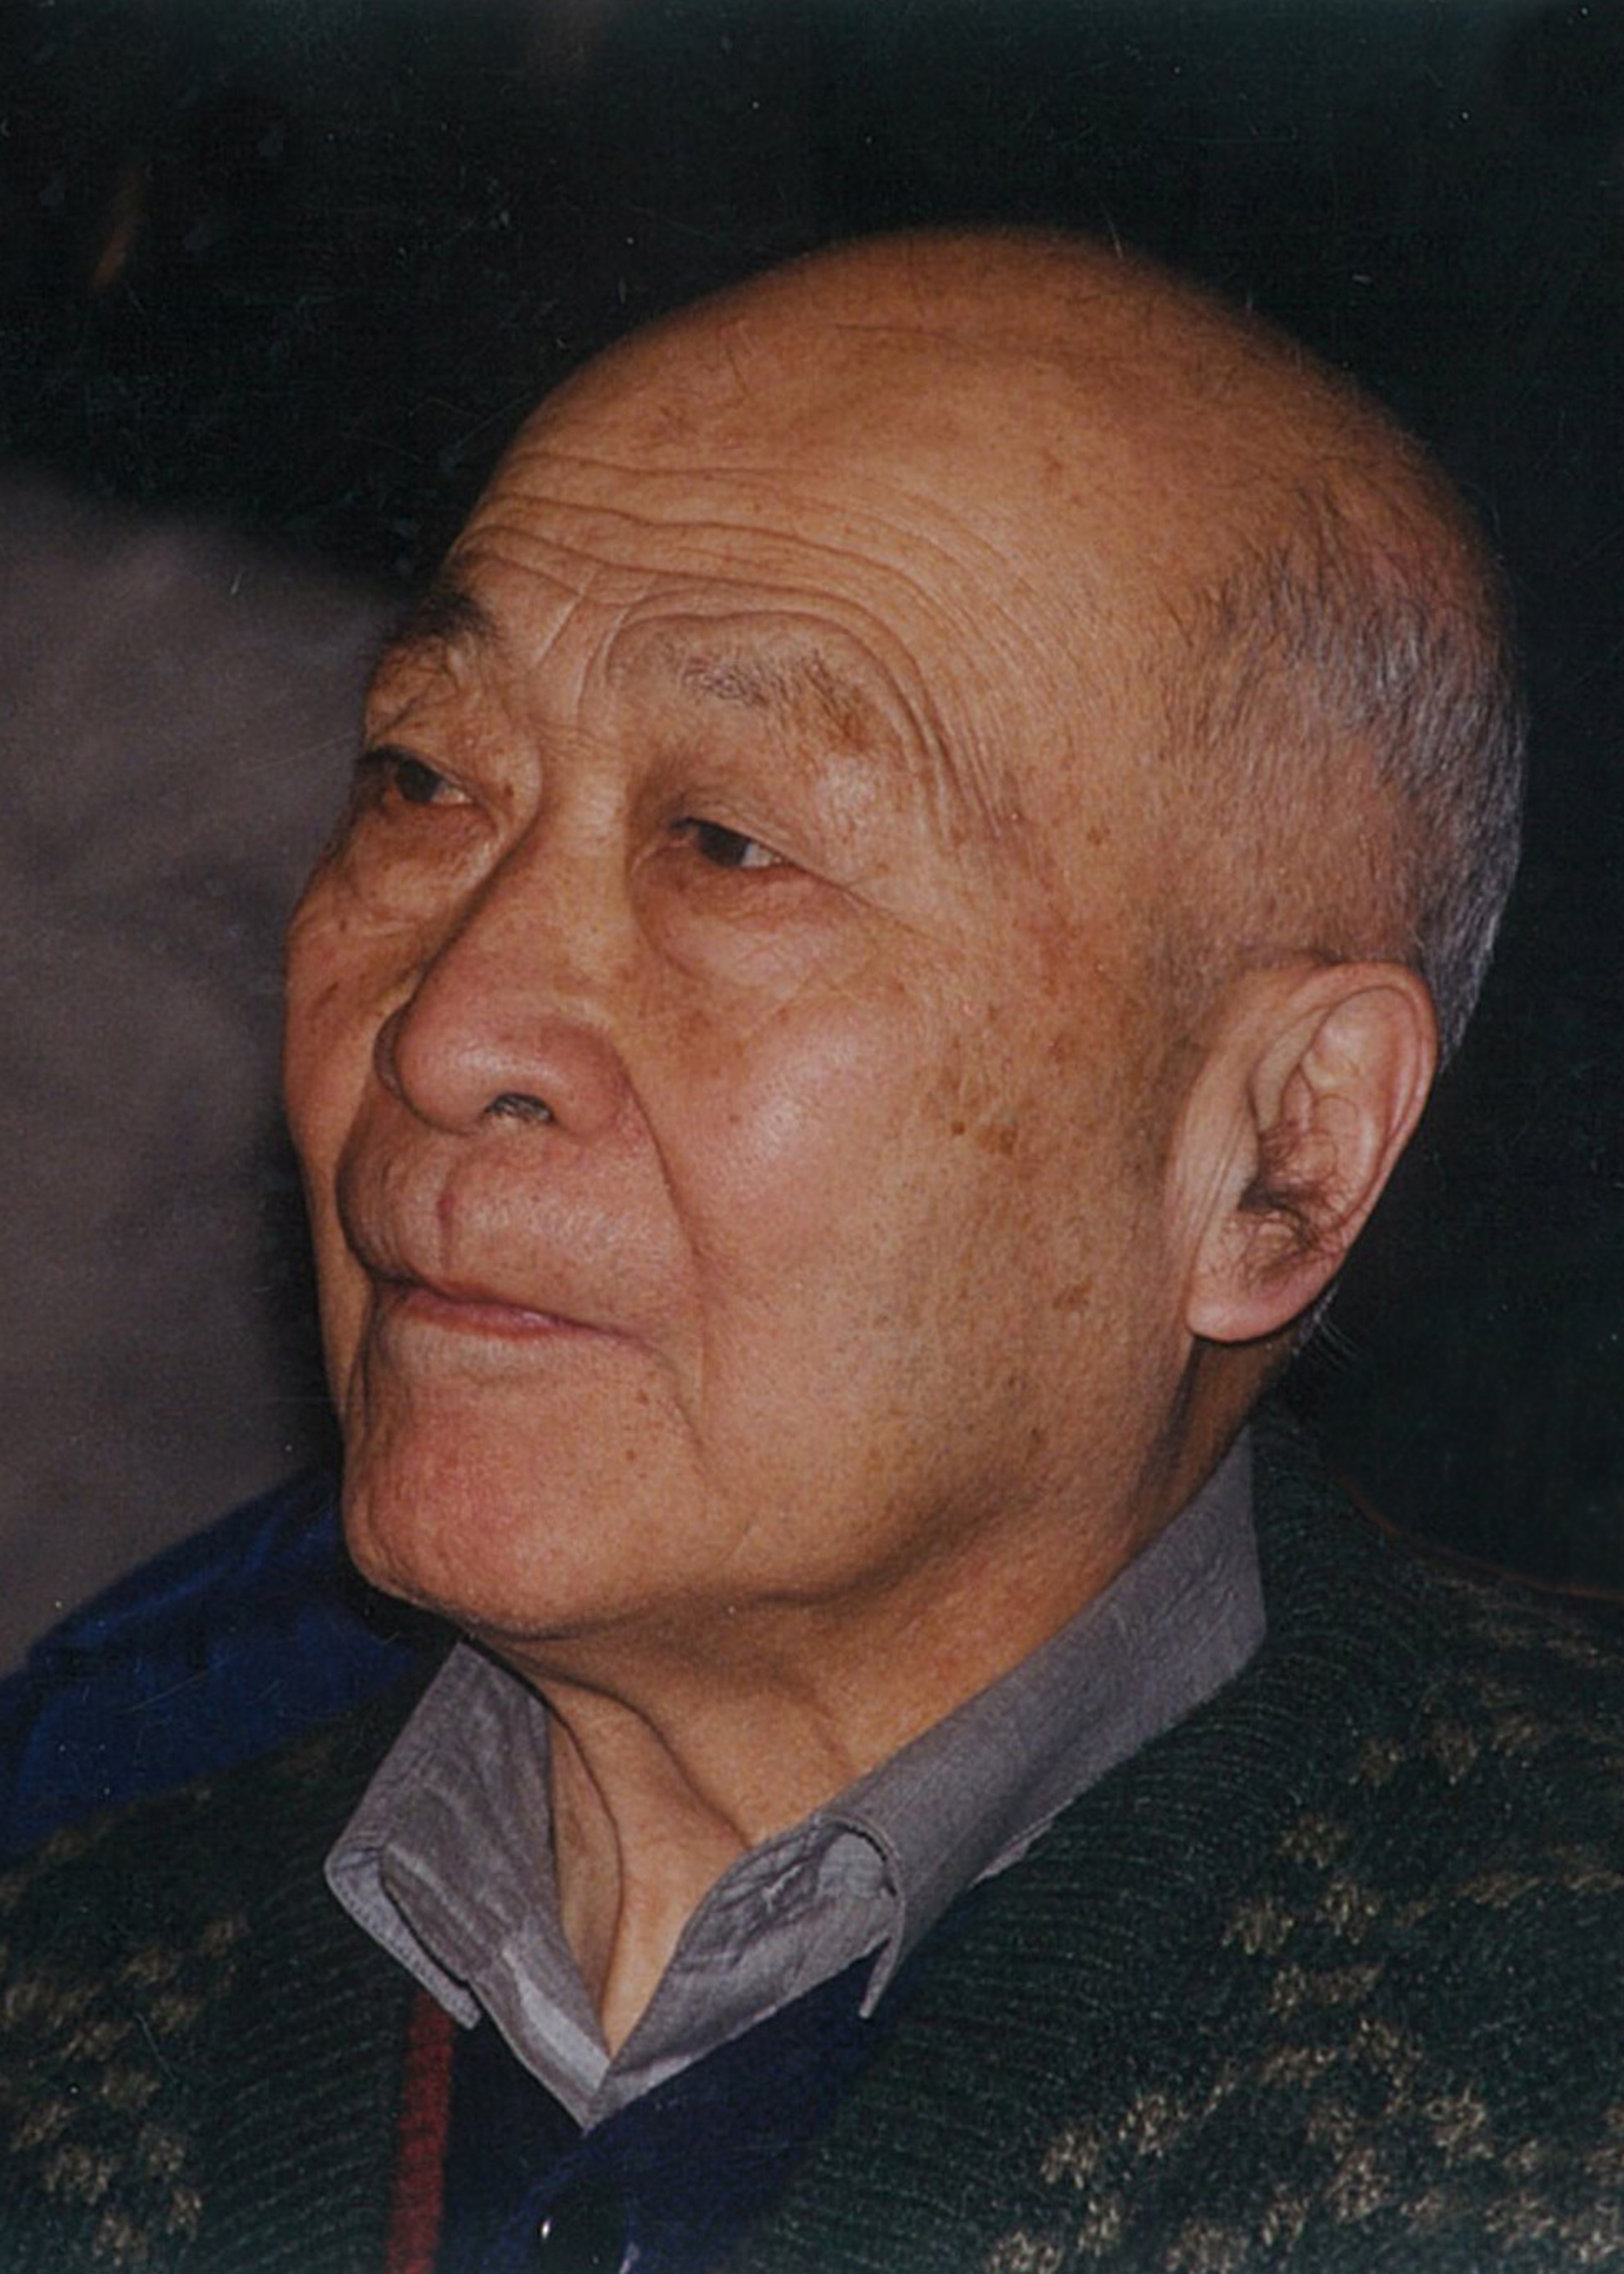
\includegraphics[height=1.20\textwidth,width=0.82\textwidth,viewport=0 0 360 520,clip]{Liu_Zengfu.jpg}
\caption*{\hei 刘曾复~教授~~(1914.11.9-2012.6.27)}
\label{Liu_Zengfu}
\end{figure}

\begin{figure}[h!]
\centering
%\vspace{+0.2in}
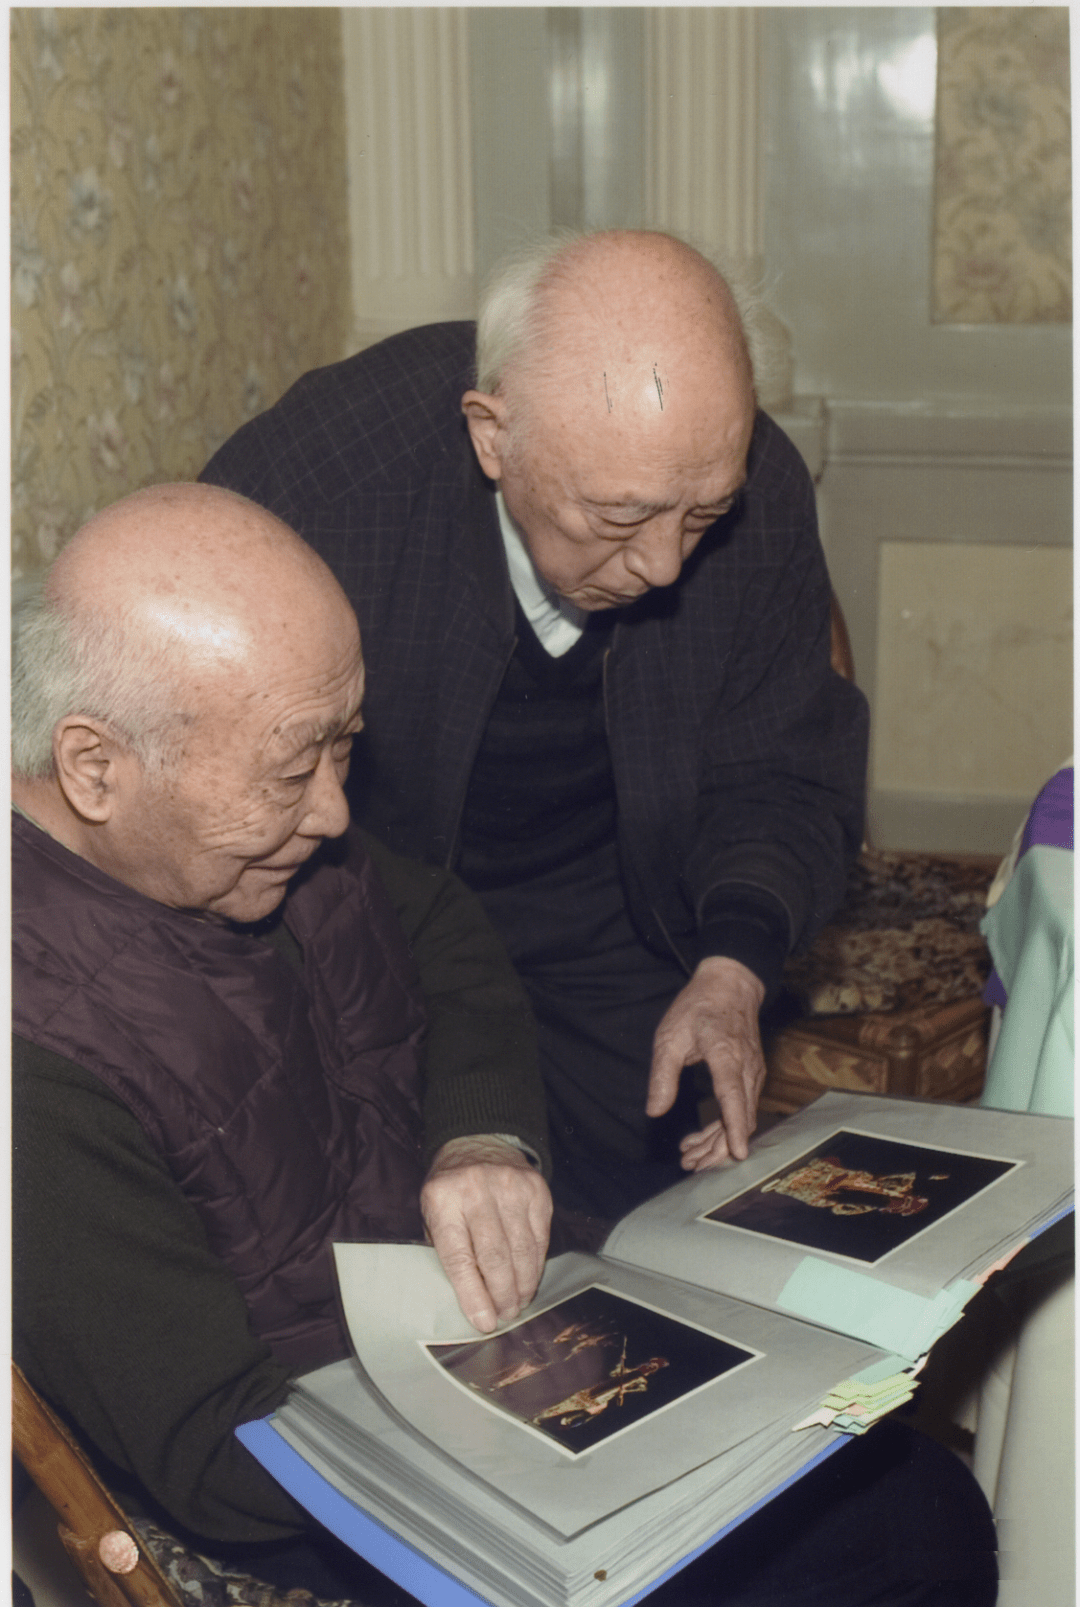
\includegraphics[height=1.38\textwidth,width=1.0\textwidth,viewport=0 0 1050 1550,clip]{Liu-Wu.png}
\caption*{\hei 刘曾复~先生~和~吴小如~先生}
\label{Collect_Liu_Wu}
\end{figure}

\begin{figure}[h!]
\centering
%\vspace{-10.5pt}
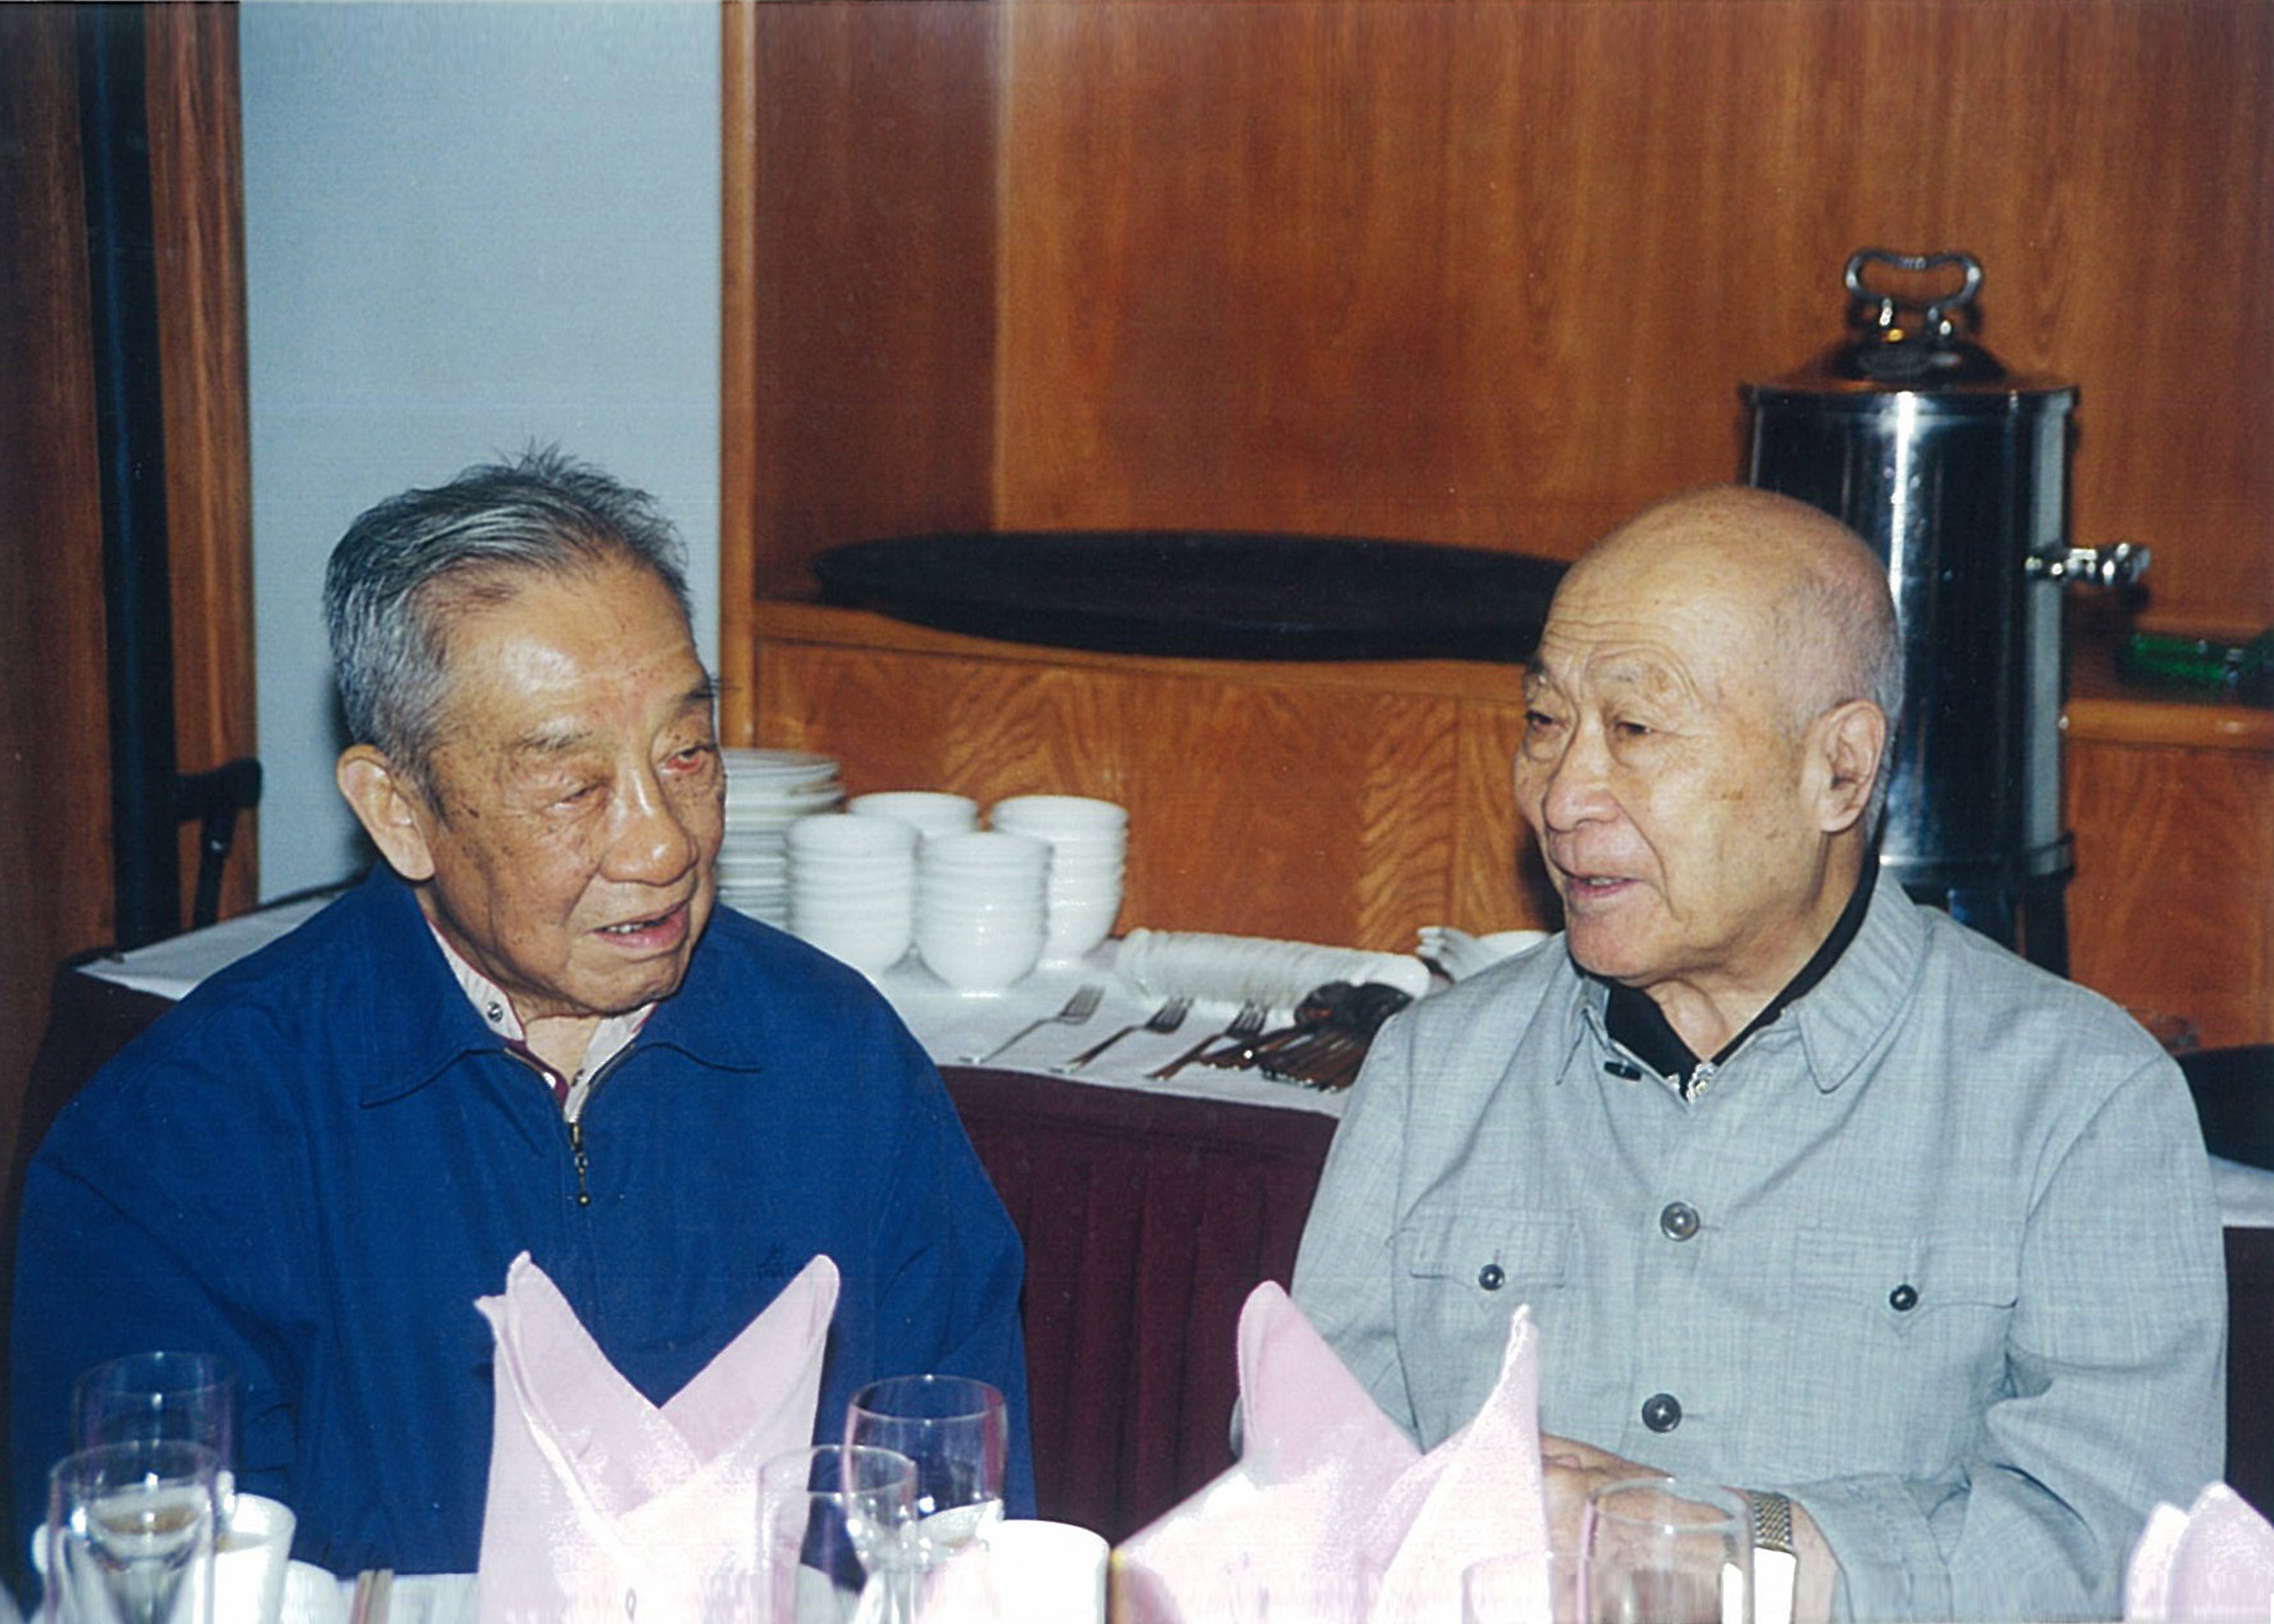
\includegraphics[height=0.60\textwidth,width=1.0\textwidth,viewport=0 0 500 300,clip]{Zhu-Liu.jpg}
\caption*{\hei 朱家溍~先生~和~刘曾复~先生}
\label{Collect_Zhu_Wu}
\end{figure}

\begin{figure}[h!]
\centering
%\vspace{-10.5pt}
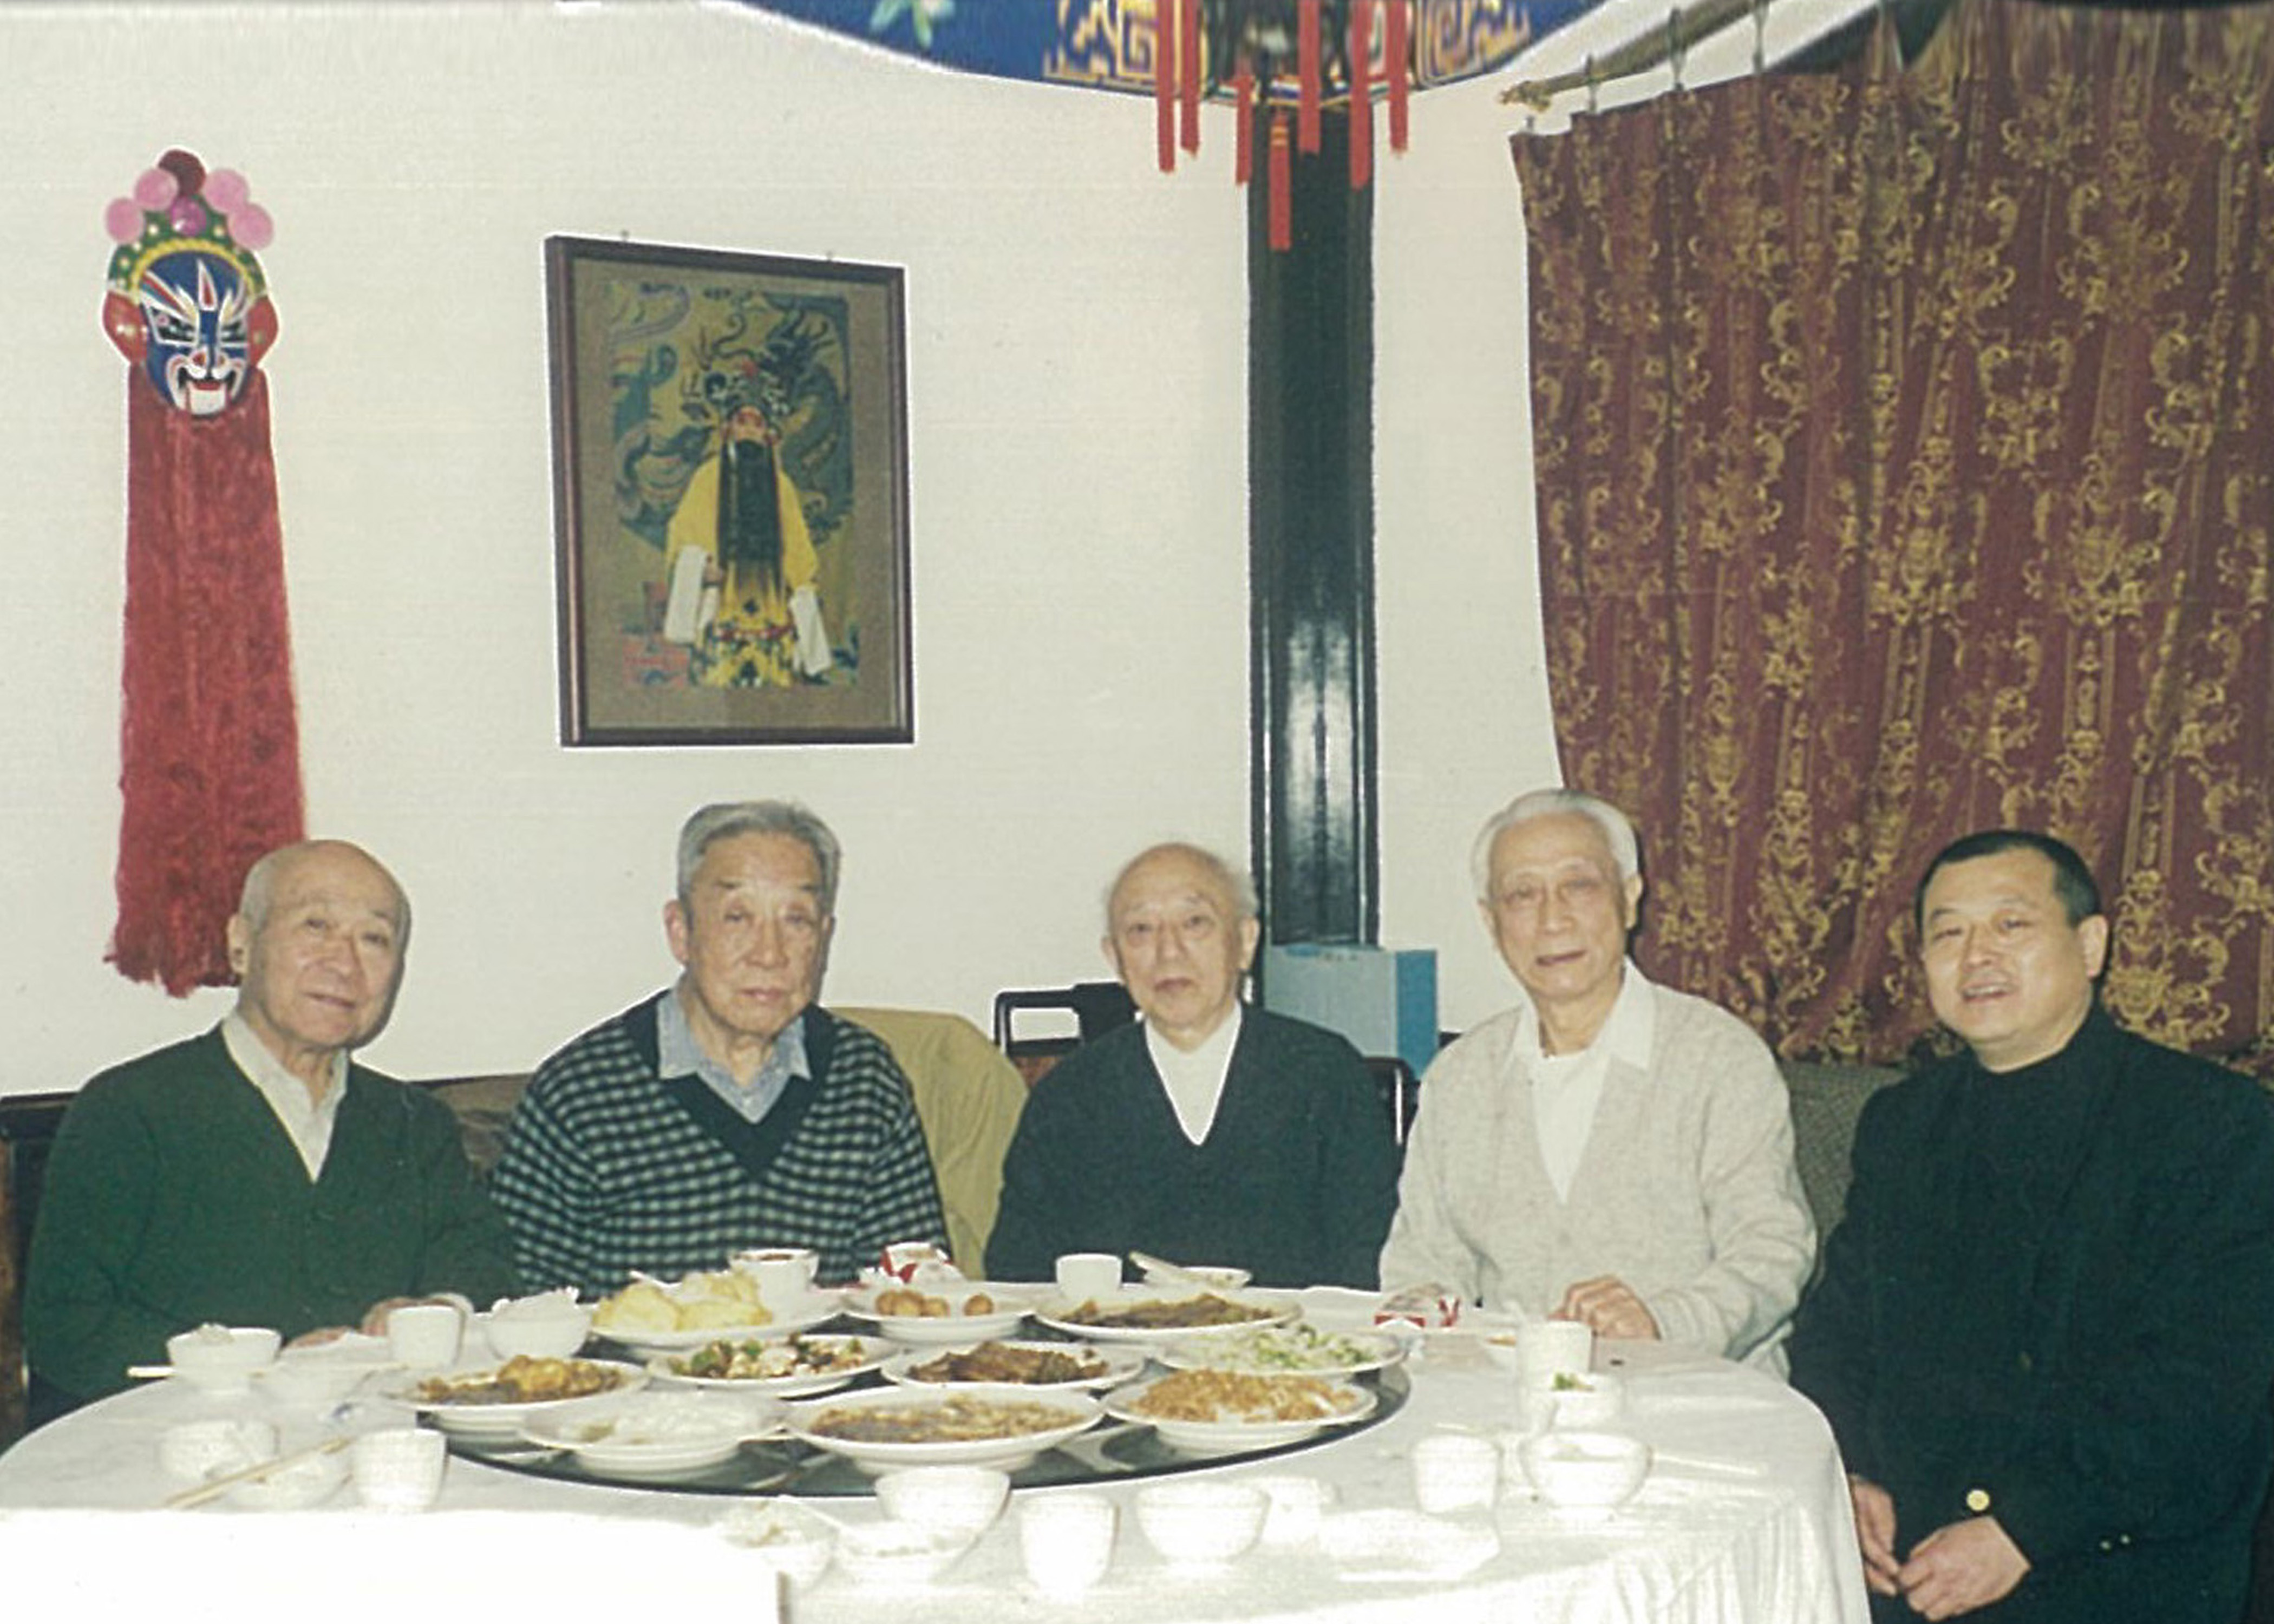
\includegraphics[height=0.60\textwidth,width=1.0\textwidth,viewport=0 0 500 300,clip]{Collect_Zhu-Liu-Wu-Wang.jpg}
\caption*{\hei 左起:~刘曾复~先生、朱家溍~先生、吴小如~先生、王金璐~先生~等~合影}
\label{Collect_Wang}
\end{figure}
%\keywords{Keyword1; Keyword2; Keyword3}

\begin{figure}[h!]
\centering
\vspace{-0.7in}
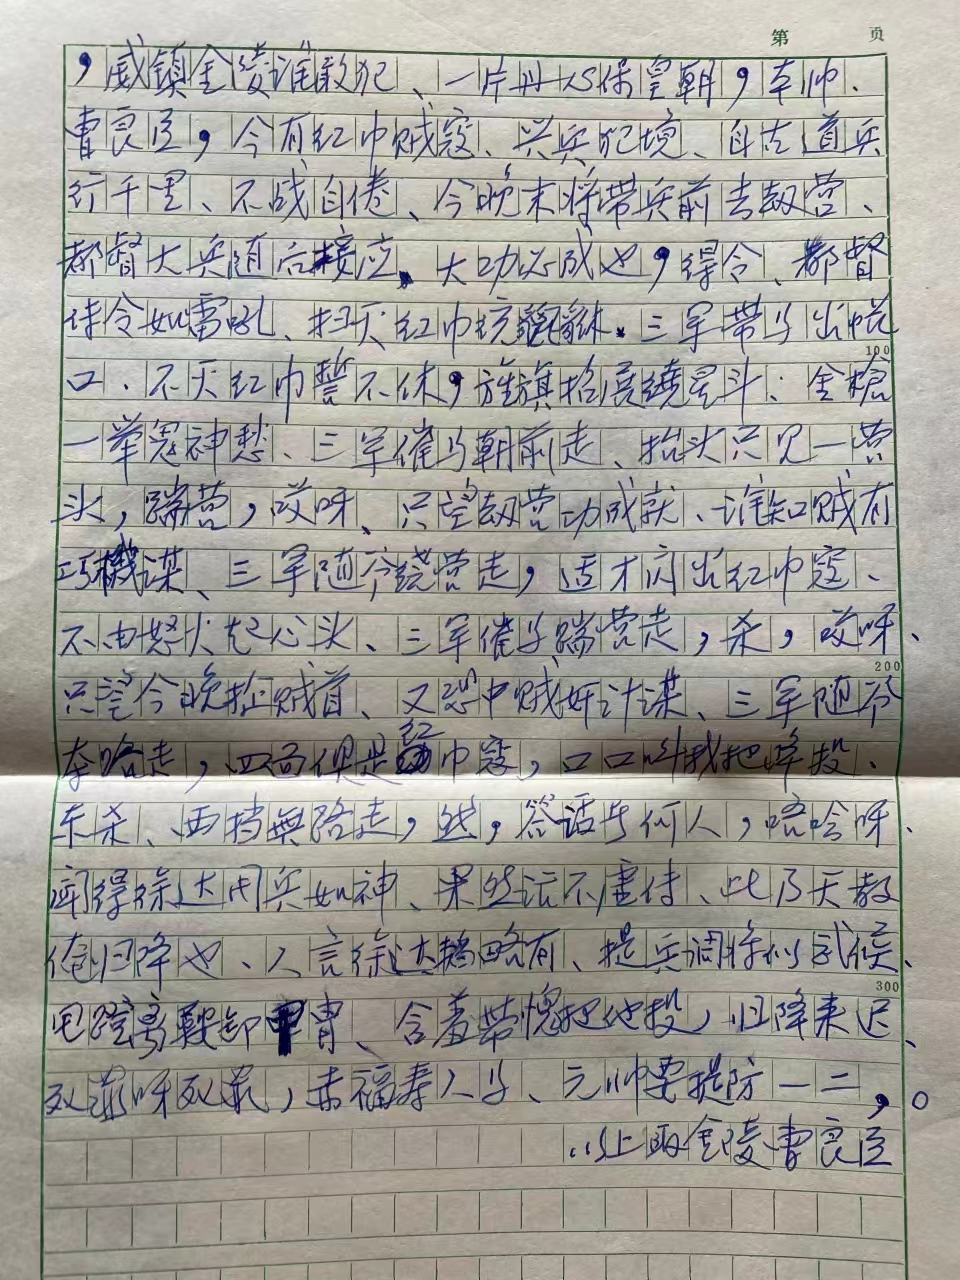
\includegraphics[height=0.68\textwidth,width=0.40\textwidth,viewport=0 0 950 1300,clip]{PekOpe_Liu-1.jpg}
\caption*{\hei 刘曾复~先生~抄录的《取金陵》曹良臣的单词}
\label{Script}
\end{figure}

\begin{figure}[hbtp!]
\hspace*{-0.5in}
\begin{minipage}[t]{0.53\textwidth}
	\centering
	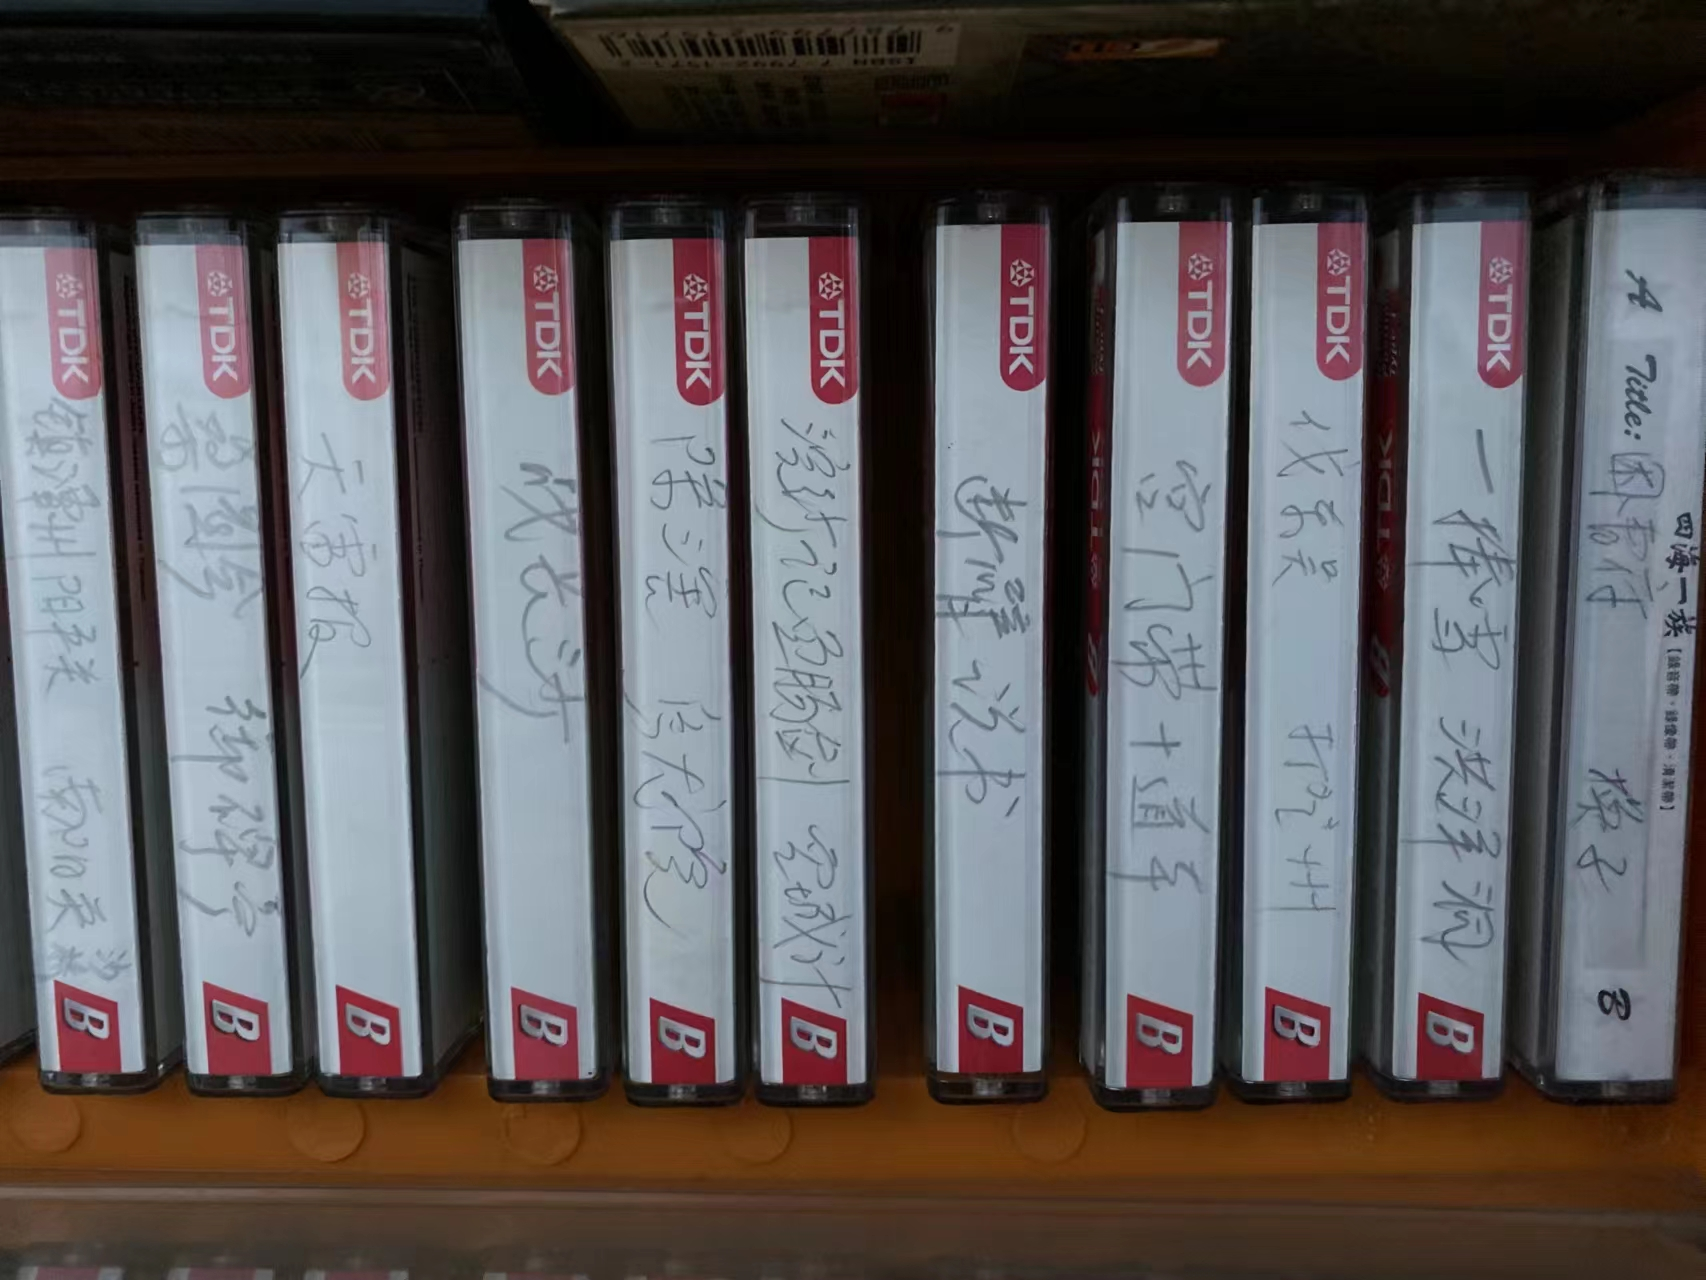
\includegraphics[height=1.00\textwidth,width=1.20\textwidth,viewport=0 0 1750 1300,clip]{PekOpe_Liu-2.jpg}
	\caption*{\hei \fontsize{8.5pt}{4.0pt}\selectfont{左:~刘曾复~先生~保存的部分说戏录音磁带}}
\end{minipage}
\hspace{0.6in}
\begin{minipage}[t]{0.43\textwidth}
	\centering
	\vspace{-3.7in}
	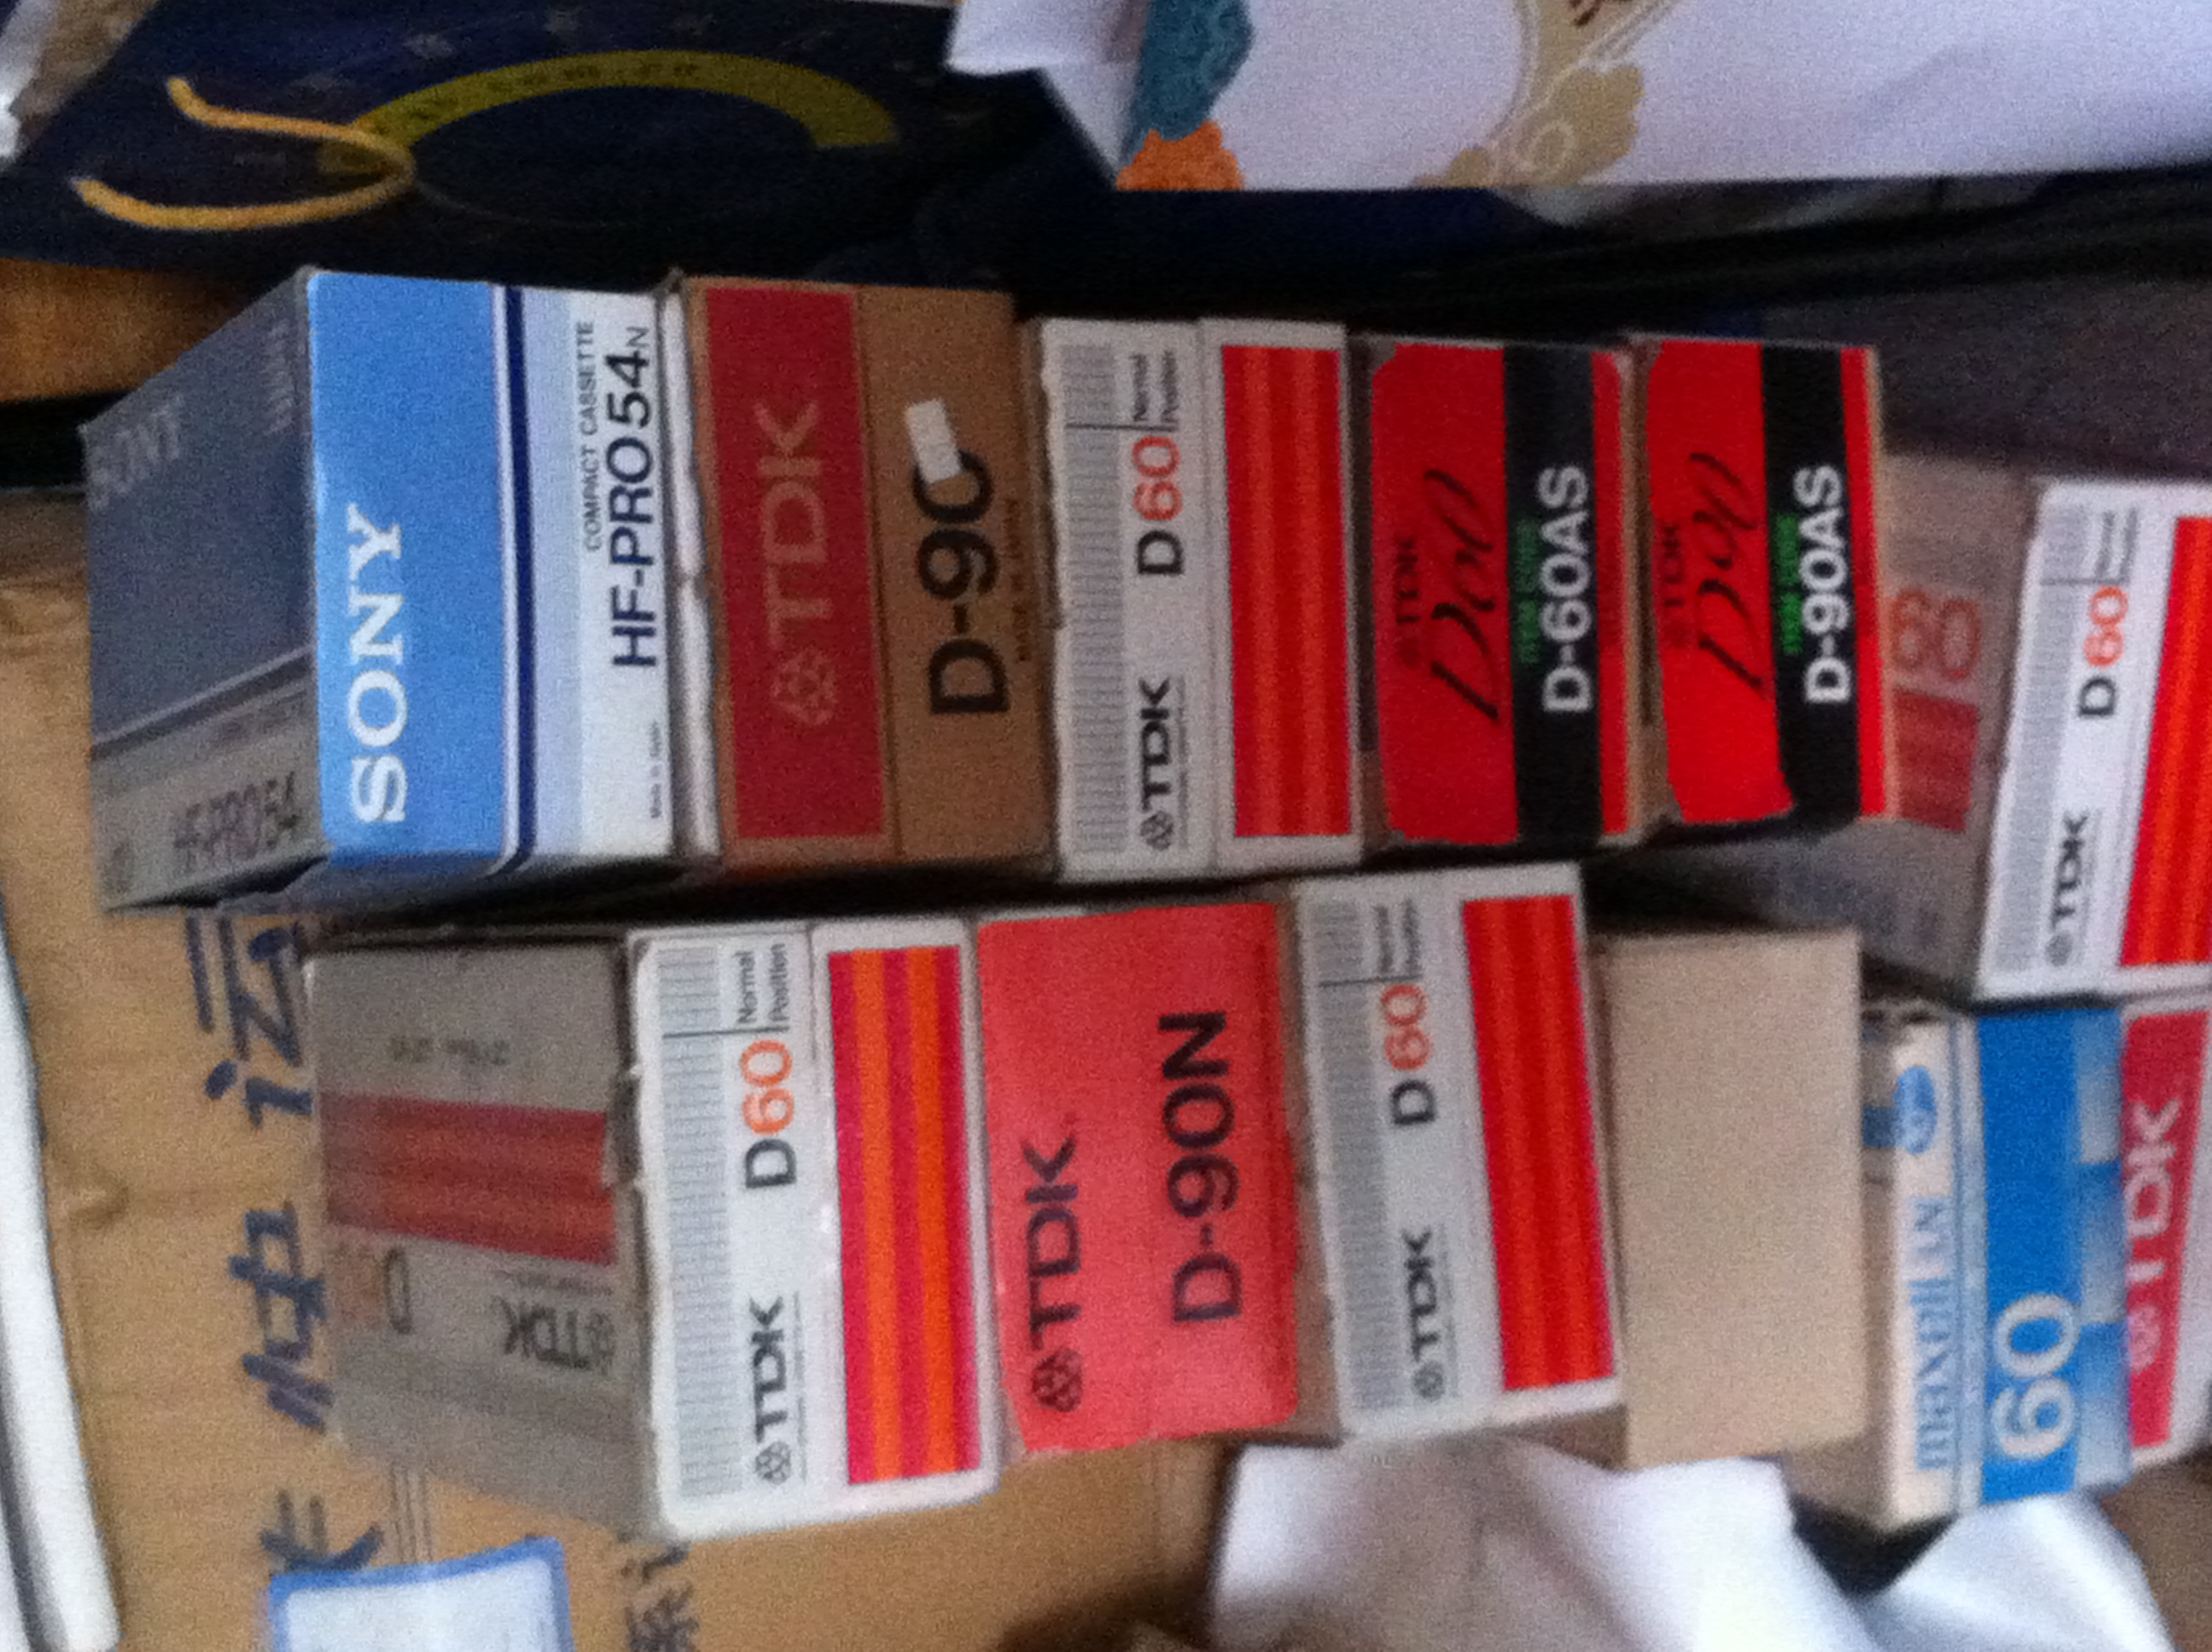
\includegraphics[height=1.10\textwidth,width=1.70\textwidth,angle=270, viewport=0 0 2750 1950,clip]{PekOpe_Wu-5.jpg}
	\caption*{\hei \fontsize{8.5pt}{4.0pt}\selectfont{右:吴小如~先生~保存的刘曾复先生的说戏录音磁带}}
\end{minipage}
\label{Records}
\end{figure}

\newpage
\setcounter{page}{0}
\pagenumbering{roman}
\hypertarget{ux8bf4-ux660e}{
\addcontentsline{toc}{subsection}{\hei 说~明}
	\subsubsection{\hei \large 说\hspace{35pt}明}\label{ux8bf4-ux660e}}
\pagestyle{fancy}    %与文献引用超链接style有冲突
\chead{说~明} % 页眉中间位置内容

\setlength{\parindent}{22pt}{     %
	此为个人整理的刘曾复教授说戏录音的文本稿,\textbf{主要根据刘曾复先生为中国戏曲学院提供的百余出说戏录音为底本,并结合刘曾老在其他场合的说戏录音}\upcite{Liu-Shuoxi-Record}%\textsuperscript{{[}1{]}}
\textbf{整理完成的}。其中《太平桥》、《盗宗卷》、《梅龙镇》、《辕门斩子》、《摘缨会》、《上天台》、《一捧雪》、《卖马》、《南阳关》的``总讲本''主要依据《京剧新序》\upcite{Liu_Xinxu-I,Liu_Xinxu-II}%\textsuperscript{{[}2{]}.}
中收录的刘曾复先生整理的剧本并结合说戏录音整理完成;《马鞍山》、《战长沙》的``总讲本''则参考了李舒先生遗作《涉艺所得》\upcite{Li-SheyiSuode}%\textsuperscript{{[}3{]}.}
收录的刘曾复先生手书稿和传本并结合说戏录音整理完成的。\textbf{有关剧目中的把子,主要摘录自}《京剧新序》和《京剧老生把子见闻录》\upcite{XQYS1-32_1983}%\textsuperscript{{[}4{]}.}
一文记录的开打和舞台调度。

除了上述《太平桥》等十一出剧目,其余剧目的场次安排主要参考了《京剧汇编~(1-109集)》\upcite{Jingju-Huibian-1}%\textsuperscript{{[}5{]}.}
、《传统剧目汇编》\upcite{Jingju-Huibian-2}%\textsuperscript{{[}6{]}.}
、《京剧丛刊~(1-50集)》\upcite{Jingju-Congkan}%\textsuperscript{{[}7{]}.}
和``中国京剧戏考''网站\upcite{PekingOpera-Scripts}%\textsuperscript{{[}8{]}.}
上的相应的剧目的安排,个别剧目的词句也参考了,``中国京剧老唱片''网站\upcite{PekingOpera-OldRecords}%\textsuperscript{{[}9{]}.}
上载的老唱片戏词。

剧目按照剧中人物年代排列,部分剧目的年代排序参考了《京剧大戏考》\upcite{Chai-DaXikao}%\textsuperscript{{[}10{]}.}
和《京剧知识词典(增订版)》\upcite{PekingOpera-Dictionary}%\textsuperscript{{[}11{]}.}
中的剧目顺序。

\vskip 5pt
基于全面、客观、忠实的记录原则,整理剧目文字的标记说明如下:
\begin{enumerate}
\def\labelenumi{\arabic{enumi}.}
\item
	{\CJKfamily{hei}因为本人学识浅陋、加之录音带存年较久,因此文字中有不少存疑处。凡是存疑处,尽量用\textcolor{red}{红色字体}标出,}表明此处可能文辞欠通顺,或只是根据字音听写臆测的词句;
\item
	{\CJKfamily{hei}刘曾复先生腹笥渊博,在不同的场合说戏时,即使是同一出戏,个别词句也略有出入,文本中尽量作了标注:~}

\begin{enumerate}
\def\labelenumi{\arabic{enumi}.}
\item
  每个剧目中凡有出入的唱、念词句标注为:

\begin{quote}
	\underline{\textrm{XX}词1}~({\akai 或}:~\textrm{XX}词2;~\textrm{XX}词3;$\cdots{}\cdots${})
\end{quote}
\begin{quote}
	\underline{\textrm{XX}句1}~({\akai 或}:~\textrm{XX}句2~{\akai 或}:~\textrm{XX}句3;$\cdots{}\cdots${})
\end{quote}

\def\labelenumi{\arabic{enumi}.}
\setcounter{enumi}{1}
\item
  每个剧目中可不念或某些衬字的唱、念标注为:

\begin{quote}
	(\textrm{XX}词句)
\end{quote}
\end{enumerate}

\def\labelenumi{\arabic{enumi}.}
\setcounter{enumi}{2}
\item
  \textbf{除``总讲本''外,``单词本''中,与表演配合的其他人物唱、念(盖口)}标记为:
\begin{quote}
	(人物\hspace{30pt} 唱、念词句\textrm{XXX}。)
\end{quote}
\item
  \textbf{在本人的知识范围内,对一些生僻的典故、词汇作了简要的注解。}
\item
  \textbf{刘曾复先生对唱、念中的虚词非常重视,文本中的虚词标注有限,建议以先生的录音为准。}
\item
  \textbf{由于文字记录的功能有限,此书辑录的主要是说戏的文字内容,关于舞台表演过程中的唱、念关键都没有标注。}
\end{enumerate}
}

%-------------------------------------------------------------------------------The Content of The Paper----------------------------------------------------------------------------------------------%
\newpage
\pagestyle{plain}   % 删除页眉                                        %
\addcontentsline{toc}{subsection}{\CJKfamily{hei} 目~录}
\tableofcontents %% 制作目录(目录是根据标题自动生成的)
%-----------------------------------------------------------------------------------------------------------------------------------------------------------------------------------------------------%

\addcontentsline{toc}{section}{\hfill[\hei 先秦·两汉]\hfill}
\newpage
\chead{先秦·两汉} % 页眉中间位置内容
\setcounter{page}{1}

\newpage
%\hypertarget{ux6e2dux6c34ux6cb3}{%
\subsubsection{\hei\large 渭水河}%\label{ux6e2dux6c34ux6cb3}}
\addcontentsline{toc}{subsection}{\hei 渭水河}

\hangafter=1                   %2. 设置从第1⾏之后开始悬挂缩进  %
\setlength{\parindent}{0pt}{
{\centerline{\textrm{{[}\hei 第一场{]}}}}
\vspace{5pt}
姬昌\hspace{30pt}~ {[}{\akai 引子}{]}为建帝基,一路平安,到西岐。

姬昌\hspace{30pt}~ ({\akai 念})纣王无道宠妲己,苦害忠良受凌逼。孤王回转西岐地,重整山河统华夷。

\setlength{\hangindent}{60pt}   %3. 设置悬挂缩进量                %
{姬昌\hspace{30pt}~ 孤,西伯侯姬昌。只因纣王无道,信宠妲己,苦害忠良,是孤回转西岐,自立基业。那日有一樵夫,名叫武吉,将孤门军\footnote{刘曾复先生说戏录音作``军门'',似非,此处从《京剧汇编》~第十三集陈少武、苏连汉~口述本。}%\protect\hyperlink{fn3}{\textsuperscript{3}}
打死,拿他问罪。他言道:~家有八旬老母,无人侍奉。孤王念他是一孝子,赐他斗米贯钱,限定七日前来抵罪,去了数十余天不见到来。我不免在八卦之中,查看吉凶。}

姬昌\hspace{30pt}~ 内侍,

内侍\hspace{30pt}~ 有。

姬昌\hspace{30pt}~ 香案伺候。

内侍\hspace{30pt}~ 香案伺候哇。

姬昌\hspace{30pt}~ 哎呀!

\setlength{\hangindent}{60pt}   %3. 设置悬挂缩进量                %
{姬昌\hspace{30pt}~ 【{\akai 二黄原板}】摇动了金钱告上苍,八卦之中显示明详\footnote{《京剧汇编》第十三集~陈少武、苏连汉~口述本~作``明祥''。}%\protect\hyperlink{fn4}{\textsuperscript{4}}
。单见单来仄见仄,查不出小武吉落于何方。}

姬昌\hspace{30pt}~ ({\akai 念})春有寅萌芽出土,夏有寅火炼金身。秋有寅黄叶落地,冬有寅滴水成冰。

\setlength{\hangindent}{60pt}   %3. 设置悬挂缩进量                %
{姬昌\hspace{30pt}~ 呜哙呀,我道此人还在,原来入土而亡。他今一死不大紧要,可叹他八旬老母,无人侍奉。唉,可叹呐可叹。}

姬昌\hspace{30pt}~ 回避了。

\setlength{\hangindent}{60pt}   %3. 设置悬挂缩进量                %
{姬昌\hspace{30pt}~ 【{\akai 二黄原板}】孤王建业在西方,只为江山昼夜忙。东路反了姜文焕,南路鄂广反陈塘。他两家俱有那书信来往,叫孤王领人马去反商王。臣反君来小犯上,倒不如稳坐西岐乐安康。移步儿\footnote{``移步儿''吴小如先生建议作``一步儿'',此处从《京剧汇编》第十三集~陈少武、苏连汉~口述本。}%\protect\hyperlink{fn5}{\textsuperscript{5}}
来至在灵台上,且做南柯梦一场。}

姬昌\hspace{30pt}~ 【{\akai 二黄导板}】孤王正在睡朦胧,

	姬昌\hspace{30pt}~ 【{\akai 二黄摇板}】只见飞熊扑帐中。手执宝剑将你斩,化阵清风无影踪。

内侍\hspace{30pt}~ 千岁醒来。

姬昌\hspace{30pt}~ ~【{\akai 二黄导板}】适才朦胧见一怪,

	姬昌\hspace{30pt}~ 【{\akai 二黄摇板}】醒来依然在灵台。

姬昌\hspace{30pt}~ 内侍。

内侍\hspace{30pt}~ 有。

姬昌\hspace{30pt}~ 宣散宜生上殿。

内侍\hspace{30pt}~ 领旨。散宜生灵台见驾。

散宜生\hspace{20pt}~ 领旨。

散宜生\hspace{20pt}~ ({\akai 念})袖里乾坤大,怀揣日月明。

散宜生 \hspace{20pt}~散宜生见驾,主公千岁。

姬昌\hspace{30pt}~ 平身。

散宜生\hspace{20pt}~ 千千岁。

姬昌\hspace{30pt}~ 赐坐。

散宜生\hspace{20pt}~ 谢坐。宣臣来见,有何圣谕?

姬昌\hspace{30pt}~ 孤王三更时分,梦一飞熊入帐,抓伤孤的左膀,不知主何吉凶?

散宜生\hspace{20pt}~ 这$\cdots{}\cdots{}$此乃大吉之兆。

姬昌\hspace{30pt}~ 怎见得?

散宜生\hspace{20pt}~ 主公传旨,郊外射猎,不得虎臣,必得良将。

姬昌\hspace{30pt}~ 先生替孤传旨。

散宜生\hspace{20pt}~ 领旨。

姬昌\hspace{30pt}~ 正是:~({\akai 念})夜梦飞熊入帐来,

	散宜生\hspace{20pt}~ ({\akai 念})郊外射猎访贤才。

\vspace{3pt}{\centerline{\textrm{{[}{\hei 第二场}{]}}}}\vspace{5pt}

武吉\hspace{30pt}~ 嗯哼!

武吉\hspace{30pt}~ ({\akai 念})胆小天下去得,刚强寸步难行。

\setlength{\hangindent}{60pt}   %3. 设置悬挂缩进量                %
{武吉\hspace{30pt}~ 小子武吉。自从那日上山砍樵,进城去卖,偶遇姬千岁门军,被我失手打死。那姬千岁拿我问罪。我曾言道:~家有八旬老母,无人侍奉。那姬千岁念我是一孝子,赏我斗米贯钱,回家见母一面,限定七日前来抵罪。不想行至渭水河边,见一老者,呃,在那里垂钓,他见我面带煞气,必有凶事。是我将打死门军之事,对他实言。他教我一个法术:~回到家中,老母床前,挖一土井,宽要七尺,深要丈二,口含灯芯、糯米,睡在井内。躲过七七四十九日,方保无事。今当四十八天,老母腹中饥饿,只得将我唤醒,命我上山砍樵,卖了钱文,买米度日。}

武吉\hspace{30pt}~ 正是:~({\akai 念})上山擒虎易,开口告人难。

\vspace{3pt}{\centerline{\textrm{{[}{\hei 第三场}{]}}}}\vspace{5pt}

	南宫适\hspace{20pt}~ \textless{}\!{\bfseries\akai 点绛唇}\!\textgreater{}扶保西岐,

北宫高\hspace{20pt}~  \textless{}\!{\bfseries\akai 点绛唇}\!\textgreater{}同心协力,

辛甲\hspace{30pt}~  \textless{}\!{\bfseries\akai 点绛唇}\!\textgreater{}立帝基,

辛免\hspace{30pt}~  \textless{}\!{\bfseries\akai 点绛唇}\!\textgreater{}四海归一,

众\hspace{41pt}~  \textless{}\!{\bfseries\akai 点绛唇}\!\textgreater{}方显英雄气。

南宫适\hspace{20pt}~ 俺,南宫适,

北宫高\hspace{20pt}~ 北宫高,

辛甲\hspace{30pt}~ 辛甲,

辛免\hspace{30pt}~ 辛免。

南宫适\hspace{20pt}~ 众位将军请了。

众\hspace{41pt}~ 请了。

南宫适\hspace{20pt}~ 主公郊外射猎,两厢伺候。

众\hspace{41pt}~ 请。

姬昌\hspace{30pt}~ ({\akai 念})旌旗遮日月,郊外访贤臣。

众\hspace{41pt}~ 参见主公。

姬昌\hspace{30pt}~ 人马可齐?

众\hspace{41pt}~ 俱已齐备。

姬昌\hspace{30pt}~ 郊外去者!

众\hspace{41pt}~ 得令。

众\hspace{41pt}~ 众将官,郊外去者。带马!

杂\hspace{41pt}~ 啊。

众\hspace{41pt}~ 前道为何不行?

杂\hspace{41pt}~ 樵夫挡道。

众\hspace{41pt}~ 人马列开!

杂\hspace{41pt}~ 樵夫当面。

武吉\hspace{30pt}~ 樵夫叩头。

姬昌\hspace{30pt}~ 下跪可是武吉?

武吉\hspace{30pt}~ 正是。

姬昌\hspace{30pt}~ 见了孤王为何不抬起头来?

武吉\hspace{30pt}~ 有罪不敢抬头。

姬昌\hspace{30pt}~ 恕你无罪。

武吉\hspace{30pt}~ 谢千岁。

姬昌\hspace{30pt}~ 呃嗯------限定七日前来抵罪。为何今日才来见孤,该当何罪?

\setlength{\hangindent}{60pt}   %3. 设置悬挂缩进量                %
{武吉\hspace{30pt}~ 千岁容禀:~那日多蒙千岁天恩,放小子回家,见母一面,不想行至渭水河边,见一老者,在那厢垂钓,他见我面带煞气,必有凶事。我将打死门军之事对他言明。他教我小小法术:~回到家去,老母床前,挖一土井,宽要七尺,深要丈二,口含灯芯、糯米,睡在其内。躲过七七四十九日,方保无事。今乃四十八日,我母不解其意,将我唤醒,命我上山砍柴,进城去卖,不想撞了\footnote{《京剧汇编》第十三集~陈少武、苏连汉~口述本~作``闯了''。}%\protect\hyperlink{fn6}{\textsuperscript{6}}
千岁御驾。唉,也是小人命该如此,情愿抵罪。}

姬昌\hspace{30pt}~ 可曾问过那渔人的名姓?

武吉\hspace{30pt}~ 这,不曾问得。

姬昌\hspace{30pt}~ 垂钓所在?

武吉\hspace{30pt}~ 渭水河边。

姬昌\hspace{30pt}~ 将柴担放下,引孤前往。

{\akai 二}太子\hspace{20pt}~ 且慢。启奏父王:~为国访贤,必须换了便服。

姬昌\hspace{30pt}~ 看衣改换。

众\hspace{41pt}~ 撒下围场。

姬昌\hspace{30pt}~ 武吉。

武吉\hspace{30pt}~ 有。

姬昌\hspace{30pt}~ 带路。

武吉\hspace{30pt}~ 领旨。

\setlength{\hangindent}{60pt}   %3. 设置悬挂缩进量                %
{姬昌\hspace{30pt}~ 【{\akai 二黄原板}】樵夫道那渔人颇有奥妙,因此上带皇儿亲走一遭。叫武吉与孤向前引道,青的山绿是水难画难描。}

\vspace{3pt}{\centerline{\textrm{{[}{\hei 第四场}{]}}}}\vspace{5pt}

\setlength{\hangindent}{60pt}   %3. 设置悬挂缩进量                %
{姜尚\hspace{30pt}~ 【{\akai 二黄原板}】纣王无道贪色酒,午门外修一座摘星楼。比干丞相遭毒手,贾氏夫人坠高楼。(我不愿在朝为官侯,隐居磻溪垂钓钩。\footnote{据段公平{\scriptsize 君}告知,原有此二句,可不唱。}%\protect\hyperlink{fn7}{\textsuperscript{7}}
) 昨夜晚在土台观看星斗,算就了西伯侯灭纣兴周。移步儿来至在渭水河口,那一边来的是西伯王侯。}

姬昌\hspace{30pt}~ ({\akai 内})武吉带路。

\setlength{\hangindent}{60pt}   %3. 设置悬挂缩进量                %
{姬昌\hspace{30pt}~ 【{\akai 二黄原板}】太平鸟不住当头叫,叫得孤王喜眉梢。土台上一道长稳坐垂钓,手执鱼竿自在逍遥。我观他倒有那仙家奥妙,想必是他腹中藏有略韬。叫武吉你与我暂且退了,二皇儿向前去细问根苗。}

{\akai 二}太子\hspace{20pt}~ 啊,那渔人请了。

姜尚\hspace{30pt}~ ({\akai 念})钓、钓、钓,大鱼不到小鱼到。用你不着,去吧。

{\akai 二}太子\hspace{20pt}~ 好生与你见礼,为何佯装不睬?

姜尚\hspace{30pt}~ ({\akai 念})从来未识金龙面,要见明君便开言。

{\akai 二}太子\hspace{20pt}~ 好大的口气。

{\akai 二}太子\hspace{20pt}~ 啊,父王,那渔翁言道:~从来未识金龙面,要见明君便开言。

姬昌\hspace{30pt}~ 呃嗯------敢是尔等轻慢于他?

{\akai 二}太子\hspace{20pt}~ 儿臣不敢。

姬昌\hspace{30pt}~ 待我向前。

姬昌\hspace{30pt}~ 啊,渔人请了。

姜尚\hspace{30pt}~ 贫道稽首。

姬昌\hspace{30pt}~ 口称``稽首'',在哪座名山修炼?

姜尚\hspace{30pt}~ 昆仑学道。稽首为尊。

姬昌\hspace{30pt}~ 在此作甚?

姜尚\hspace{30pt}~ 在此垂钓。

姬昌\hspace{30pt}~ 钓得何鱼?

姜尚\hspace{30pt}~ 西海鳌鱼。

姬昌\hspace{30pt}~ 小小竹竿,焉能钓得鳌鱼?

姜尚\hspace{30pt}~ 竹竿虽小,能坠千斤。

姬昌\hspace{30pt}~ 借来一观。

姜尚\hspace{30pt}~ 请看。

姬昌\hspace{30pt}~ 呜哙呀!为何用直钩垂钓?

姜尚\hspace{30pt}~ 贫道心直性直,故而用直钩垂钓,有道是``愿者上钩''。

姬昌\hspace{30pt}~ 但不知谁愿谁不愿?

姜尚\hspace{30pt}~ ({\akai 念})耐烦等到群鱼到,自有鱼儿来吞钩。

姬昌\hspace{30pt}~ 请问渔人尊姓大名?

姜尚\hspace{30pt}~ 贫道姓姜名尚字子牙。

姬昌\hspace{30pt}~ 道号?

姜尚\hspace{30pt}~ 飞熊。

姬昌\hspace{30pt}~ ``飞熊''!应孤梦兆也。

姜尚\hspace{30pt}~ 来者上姓?

姬昌\hspace{30pt}~ 在下西伯侯姬昌。

姜尚\hspace{30pt}~ 哦,原来是姬千岁,失敬了。

姬昌\hspace{30pt}~ 岂敢。

姜尚\hspace{30pt}~ 不在西岐,来在渭水则甚?

姬昌\hspace{30pt}~ 特请先生,扶保姬氏河山。

姜尚\hspace{30pt}~ 贫道才疏学浅,不敢当此重任。

姬昌\hspace{30pt}~ 先生不必推辞。

姬昌\hspace{30pt}~ 武吉。

武吉\hspace{30pt}~ 在。

姬昌\hspace{30pt}~ 封你开路先锋,准备车辇伺候。

武吉\hspace{30pt}~ 遵命。

武吉\hspace{30pt}~ ({\akai 念})不是姜太公,怎能作先锋。

姬昌\hspace{30pt}~ 请先生转至大营。

姜尚\hspace{30pt}~ 请。

姬昌\hspace{30pt}~ 【{\akai 二黄原板}】久闻先生今相见,

姜尚\hspace{30pt}~ 【{\akai 二黄原板}】姜子牙八十二才遇名贤。

姬昌\hspace{30pt}~ 【{\akai 二黄原板}】孤王江山全仗你,

姜尚\hspace{30pt}~ 【{\akai 二黄原板}】要保江山万万年。

\vspace{3pt}{\centerline{\textrm{{[}{\hei 第五场}{]}}}}\vspace{5pt}

\textrm{武吉\hspace{30pt}~ 启千岁:~车辇齐备。}

\textrm{姬昌\hspace{30pt}~ 请先生登辇。}

\textrm{姜尚\hspace{30pt}~ 贫道有僭了。}

\textrm{姜尚\hspace{30pt}~ 【{\akai 西皮导板}】听号炮三声响旌旗招展,}

\setlength{\hangindent}{60pt}   %3. 设置悬挂缩进量                %
{\textrm{姜尚\hspace{30pt}~ 【{\akai 西皮原板}】满营中众将官齐跨雕鞍。对主公施一礼忙登车辇,姜子牙坐车辇细把君观:~前三皇后五帝年深日远,有尧、舜并禹、汤四大名贤。西伯侯夜得兆飞熊扑面,散宜生奏一本【{\footnotesize 转}{\akai 西皮快板}】郊外访贤。打柴汉名武吉引君来见,姜子牙八十二才遇名贤。行八百单八步住了车辇,}}

\textrm{姜尚\hspace{30pt}~ 【{\akai 西皮摇板}】到后来保周室八百八年。}

\textrm{武吉\hspace{30pt}~ 启千岁:~西岐众百姓,头顶香盘,迎接千岁、先生进城。}

\textrm{姬昌\hspace{30pt}~ 香盘撤去,摆队进城。}

\textrm{武吉\hspace{30pt}~ 香盘撤去,摆队进城。}
}



\textbf{焚烟墩·挡幽}\protect\hyperlink{fn8}{\textsuperscript{8}}

\textbf{(}【\textbf{大锣长锤}】,四绿龙套手拿月华旗,两个旗牌,上,站门\textbf{)}

(申侯上,\textbf{``}九龙口\textbf{''}旁,起唱\textbf{)}

\textbf{申侯 【西皮三眼】周天子行无道难逃我手,}

(申侯至台中央,接唱,\textbf{``}扯四门\textbf{''})

\textbf{申侯
【西皮三眼】先帝呀爷他封我申地为侯。恨昏王废太子贬了申后,因此上领人马扎至山头(或:扎至山口)。将人马埋伏在三岔路口哇,}

\textbf{申侯 【西皮摇板】等昏王到此来细问根由。}

\textbf{申侯 大路埋伏,小路放起烟火,君妃到此(或:昏王到此),速报我知。}

\textbf{众 啊!}

(申侯下,四个龙套拿月华旗在后场,\textbf{拉起成阵墙})

(幽王、褒姒上)

\textbf{幽王 【西皮导板】直杀得气冲天如同白昼,}

\textbf{幽王 哎呀(或:罢)!}

\textbf{(幽王和褒姒到小边,幽王要摔倒,褒姒搀扶)}

\textbf{褒姒 万岁怎么样了?}

\textbf{幽王 唉!}

\textbf{(褒姒搀幽王,幽王接唱,在月华旗前``}扯四门\textbf{'')}

\textbf{幽王 【西皮原板】遭不幸尸堆山血水倒流。}

\textbf{(幽王至小边)}

\textbf{幽王
【西皮原板】千层浪翻身转慈航搭救,王虽然得活命}龙落孤洲\textbf{。皆因是孤有错说不出口,都只为你进宫起祸根由。悔不该听奸臣【转西皮快板】谗言启奏,悔不该把朝事一旦抛丢。悔不该废太子又贬申后,悔不该与国舅结下冤仇。悔不该在骊山【转西皮快板】取乐饮酒,悔不该焚烟墩戏耍诸侯。看起来孤的命------}

\textbf{幽王 嘿------呀!}

\textbf{幽王 【西皮摇板】只怕是断送在你手,}

\textbf{褒姒 万岁命丧我手(或:万岁命丧奴手),唉!待我死了罢!}

\textbf{幽王 唉呀嚯,舍不得哟! (或:慢来慢来,还舍不得哟!)}

\textbf{(幽王、褒姒至小边)}

\textbf{幽王
【西皮摇板】劝梓童休伤悲且免忧愁。被西戎杀得孤无处逃呃走,三岔口迷了路不能相投。}

\textbf{幽王 梓童,(你我)失迷路途,待孤探路。}

\textbf{褒姒 小心了。}

\textbf{幽王 (呃,)晓得哟。}

\textbf{幽王
【西皮摇板】这一阵杀得孤魂飞胆丧,西戎兵一个个四路埋藏。又只见杏黄旗空呃中飘哇荡,倘若是遇仇敌孤命残伤。}

\textbf{(幽王看``申''字大旗)}

\textbf{(幽王 啊------)}

\textbf{幽王
【西皮摇板】上写着是申侯要除无道,拿住了小周王(或:小昏王)定斩不饶。}

\textbf{众 君王到。}

\textbf{(\textless{}急急风\textgreater{},}四个龙套拿\textbf{月华旗撤到大边,斜向,后面摆桌子、椅子,申侯坐桌上,子午相。两个旗牌分别站在桌子两旁的椅子上)}

\textbf{申侯
【西皮导板】听说是小昏王(或:听说是小周王)君妃驾到(或:君妃来到),}

\textbf{申侯
【西皮原板】正要他到此来细问根苗。权作了痴呆汉我佯装不哇晓,是何方反贼兵身穿龙袍。}

\textbf{幽王 贤侯!}

\textbf{幽王
【西皮原板】尊贤侯你那里未必不晓,孤就是周天子逃难荒郊。皆因是孤无道命运不好,看起来孤倒运还是孤八字不高(或:看起来算是孤八字不高)。}

\textbf{申侯
【西皮原板】你既是周天子福分非小(或:八字非小;八字不小),你就该在宫中快乐逍遥。这是你人背时八字不好(或:命运不好),看起来天有眼报应在今朝。}

\textbf{幽王
【西皮原板】尊贤侯你心下不必计较,孤有言你那里细听根苗:望贤侯保孤回重重相报,孤封你世代公侯与孤王同掌九朝。}

\textbf{申侯
【西皮原板】听他言不知羞令人呃可笑,我正要保你回同掌九朝。回宫去与奸妃把酒色贪好,你还把朝纲事一旦丢抛。}

\textbf{申侯 那土台之上,坐一女子,身穿大红,怀抱婴儿,她是何人?}

\textbf{幽王
那就是褒姒娘娘,怀抱婴儿是孤的爱子名叫伯服。啊,梓童,上得前去端端正正见上一礼,他保你我君妃回朝也未可知。}

\textbf{(\textless{}行弦\textgreater{}幽王示意褒姒行礼)}

\textbf{(褒姒 奴惧呀。)}

\textbf{(幽王 你要去呀。)}\protect\hyperlink{fn9}{\textsuperscript{9}}

\textbf{(幽王嗔介)}

\textbf{褒姒 是。}

\textbf{褒姒 申侯------万福!}

\textbf{申侯 好个褒娘娘正宫主呃母(或:正宫国母)!}

\textbf{申侯
【西皮原板】恨奸妃不行善你又不行好,无端地害吾妹天理自昭。每日呀里与昏王酒色欢好,你可知申正宫她与我一母同胞。}

\textbf{褒姒
【西皮原板】申国母待小奴恩高义好,我岂肯将她人一旦丢抛。望贤侯看薄面把君妃来保,早烧香晚点灯答报恩高。}

\textbf{申侯
【西皮原板】我自然保他回【转西皮快板】看你的金面,为什么废太子上欺青天。叫人来准备下麻绳、铁链,不论君、不论妃锁拿军前。拿住了小昏王(或:拿住了小周王)大功来建,若有人违将令斩罪无宽。}

\textbf{幽王
【西皮原板】你那里要我命不敢强辩,哭干了黄河水难保命还。依然是申国母独掌宫院,我和你郎舅情结什么仇冤。}

\textbf{申侯
【西皮摇板】小昏王(或:教昏王)休得要巧言舌辩,待我将十条罪细表根源:}

\textbf{申侯
【西皮二六】一条罪初登基民女挑选,二条罪老王薨作乐喧天。三条罪废国母宫闱混乱,四条罪宠尹球灭忠害贤。五条罪命石父}\protect\hyperlink{fn10}{\textsuperscript{10}}\textbf{【转西皮快板】兴兵发难,六条罪把朝纲丢在一边。七条罪弃太子纲常败乱(或:纲常大变),八条罪宠奸妃诡计多端。九条罪在骊山君妃饮宴,十条罪焚烟墩戏耍群贤。你为君十条罪人心涣散,死九泉见先王有何话言。}

\textbf{幽王
【西皮摇板】大不该在骊山作乐饮宴,大不该焚烟墩戏耍群贤。你本是大丈夫英雄好汉,杀了我无用人你算什么能员。}

\textbf{褒姒
【西皮摇板】听他言不由我心中好惨,做一朝人王主这样凄然。眼见得君妃们不能回转,}

\textbf{褒姒 \textless{}哭头\textgreater{}万岁呀!}

\textbf{褒姒 【西皮摇板】我和你就死在燃眉之间。}

\textbf{褒姒 喂呀,万岁呀\ldots{}\ldots{}(哭介)}

\textbf{申侯
【西皮摇板】又只见他君妃哭得好惨,杀君王犹如那子杀父般。叫三军(或:叫人来)放开路任他逃散(或:容他逃窜;容他逃散;任他逃窜),落一个忠义名万载流传。}

\textbf{幽王
梓童,此乃一字长蛇阵,有放你我君妃之意,我们走了罢(或:我们溜了罢)。}

\textbf{褒姒 (唉,)逃了罢(或:走了罢)。}

\textbf{幽王 溜了罢。}

\textbf{(幽王在大边唱)}

\textbf{幽王
【西皮摇板】孤回朝(或:孤还朝)有一日登了大宝,捉住了这申侯(或:捉住了小申侯)万剐千刀。}

\textbf{幽王 我们走了罢。}

\textbf{众 幽王逃走。}

\textbf{申侯 带马!}

\textbf{(旗牌下去,四绿龙套站门,带马,申侯上马)}

\textbf{申侯
【西皮快板】非是我放开路任他逃窜(或:与他逃窜),到前面}\protect\hyperlink{fn11}{\textsuperscript{11}}\textbf{遇戎兵难逃命还。教三军------}

\textbf{众 有!}

\textbf{申侯 【西皮摇板叫散】你与爷(或:你与我)忙往前趱呐,}

\textbf{(两个旗牌在小边,申侯大边)}

\textbf{申侯 【西皮散板】做一个哇假人情顺呃水推船。}

\textbf{(申侯举马鞭,台口亮相,绕一圈,打马下)}

\textbf{本戏人物扮相}:

申侯 绿蟒,黑三,戴侯帽,不挎宝剑。

幽王
大白粉脸,黑嘴窝,黑满,不戴帽,戴发鬏,穿黄团龙帔。\protect\hyperlink{fn12}{\textsuperscript{12}}

褒姒 不戴凤冠,穿黄帔。

龙套 四名(一堂),俱穿绿。

旗牌 两名,俱穿黄;一个戴髯口,一个不戴髯口。

\newpage
\hypertarget{ux5b5dux611fux5929-ux4e4b-ux5171ux53d4ux6bb5}{%
\subsection{\texorpdfstring{孝感天\protect\hyperlink{fn13}{\textsuperscript{13}}
之
共叔段}{孝感天13 之 共叔段}}\label{ux5b5dux611fux5929-ux4e4b-ux5171ux53d4ux6bb5}}

{[}第一场{]}

(\textless{}\textbf{大锣打上}\textgreater{}四龙套拿云牌上,站门,共叔段\protect\hyperlink{fn14}{\textsuperscript{14}}、卫云环同上,到台中间)

共叔段 (念)丹心天地惨,黄泉路途遥。

(卫云环
(念)溺爱反遭害,恩情一旦抛\protect\hyperlink{fn15}{\textsuperscript{15}}。)

共叔段
吾乃共叔段鬼魂\protect\hyperlink{fn16}{\textsuperscript{16}}是也。

(卫云环
吾乃卫云环鬼魂是也\protect\hyperlink{fn17}{\textsuperscript{17}}。)

共叔段
生前吾母爱子爱媳,反误我夫妻性命。闻得吾母在颖地之中,思儿想媳,不免前去探望一番。\protect\hyperlink{fn18}{\textsuperscript{18}}

共叔段、卫云环 请。

共叔段
正是:(念)蜀魄啼残三月雨\protect\hyperlink{fn19}{\textsuperscript{19}},

(卫云环
(念)梦魂惊断五更风\protect\hyperlink{fn20}{\textsuperscript{20}}。)

(\textless{}\textbf{大锣打下}\textgreater{}四龙套下,共叔段、卫云环下,\textless{}\textbf{撤锣}\textgreater{})

{[}第二场{]}

(\textless{}\textbf{小锣打上}\textgreater{}二宫女上,站门,姜氏上)

(姜氏 {[}引子{]} 身居颖地,思娇儿,珠泪双悲。)

(姜氏坐小座)

(姜氏 (念)生离最是苦,死后何伤乎!世看姜国母,有子不如无。)

(姜氏
哀家姜皇后,只因溺爱次子共叔段,反累夫妇双亡。可恨寤生,将我迁入颖地居住。思想起来,好不伤惨人也。)

(\textless{}\textbf{扎多乙}\textgreater{})

(姜氏
【二黄原板】姜国母在颖地长吁短叹,思皇儿昼夜里珠泪不干。恨寤生他与我母子情断,但不知何日里得转故园。)

(\textbf{起更},姜氏站起,\textless{}\textbf{小拉子}\textgreater{},姜氏脱黄帔)

(姜氏 回避了。)

(二宫女翻下)

(姜氏 【二黄慢板】居深宫冷清清无依无伴,
怕只怕睡不安月照栏杆。对银灯眼昏花思自叹,)

(姜氏进桌子)

(姜氏 【二黄慢板】有谁人怜念我影孤形单。)

(\textless{}\textbf{长锤}\textgreater{},共叔段上,卫氏同随上,同站小边台口)

共叔段 【二黄慢板】风飘飘冷飕飕黄昏惨淡, 曾记得在生时束带顶冠。

(共叔段挖门进,站大边,朝里)

(卫云环 【二黄慢板】此时间讲什么粉消香散,
进寝宫(或:进宫去)愿母后免去心酸。\protect\hyperlink{fn21}{\textsuperscript{21}})

(卫云环挖门进,站小边,朝里)

共叔段
\textless{}\textbf{双叫头}\textgreater{}母亲!老娘啊!\ldots{}\ldots{}(哭介)

(卫云环
\textless{}\textbf{双叫头}\textgreater{}母后!婆母!喂呀\ldots{}\ldots{}(哭介))\protect\hyperlink{fn22}{\textsuperscript{22}}

(姜氏 【反二黄导板】梦儿里又听得有人呼唤,)

(姜氏 【反二黄摇板】又只见灯光下双影闪闪。看不明抚一抚昏花老眼,)

共叔段 母亲啊\ldots{}\ldots{}(哭介)

(卫云环 母后,喂呀\ldots{}\ldots{}(哭介))

(\textless{}\textbf{凤点头}\textgreater{})

(姜氏 【反二黄摇板】却原来子叔段、儿媳云环。
曾记得寿宴前(或:曾记得寿筵前)金樽酒满,
你夫妻双双拜母子同欢。自从儿到京都未能相见,)

(起反二黄【回龙】)

共叔段、卫云环
【回龙】尊国母且不必双目泪涟\protect\hyperlink{fn23}{\textsuperscript{23}}。

共叔段 【反二黄慢板】悲切切尊国母魂飞魄散,
悔不该图兄位自惹身残。辜负了生身母无依无伴,
儿死在黄泉路也难心甘。\protect\hyperlink{fn24}{\textsuperscript{24}}

(卫云环
【反二黄慢板】这也是天命定数有修短,劝国母切莫言终日泪涟。为报恩来世里重会慈范,千古来有谁人百岁同欢。\protect\hyperlink{fn25}{\textsuperscript{25}})

(姜氏
【反二黄原板\protect\hyperlink{fn26}{\textsuperscript{26}}】听他言不由我心中悲惨,原来是我的儿站在面前。莫非是母子们梦里相见,纵然是梦相会娘也心甘。)

(叫散,\textless{}\textbf{扭丝}\textgreater{}\textless{}\textbf{凤点头}\textgreater{})\protect\hyperlink{fn27}{\textsuperscript{27}}

共叔段
【反二黄摇板】娘在阳儿在阴两厢隔断,母子们要相逢(或:要相会;要重逢)梦里团圆。\protect\hyperlink{fn28}{\textsuperscript{28}}

(共叔段出门,下)

(卫云环
【反二黄摇板】天将明儿要归不必怜念,指日里郑君侯迎请凤鸾。\protect\hyperlink{fn29}{\textsuperscript{29}})

(卫云环出门,下。五更,亮更\protect\hyperlink{fn30}{\textsuperscript{30}},二宫女上)

(二宫女 国太醒来。)

(姜氏 【二黄导板】适才间见娇儿肝肠痛断,)

(姜氏 儿啊\ldots{}\ldots{}(哭介))

(姜氏出位,站在桌前)

(姜氏 【二黄摇板】醒来时却原来南柯梦间。相劝我好言语甚是悲惨,)

(二宫女扯斜)

(姜氏 【二黄摇板】等候了郑君侯接我回还(或:接我回銮)。)

(姜氏 唉,儿啊\ldots{}\ldots{}(哭介))

(姜氏下,二宫女随下)

\textbf{剧中人物扮相:}

共叔段: 戴紫金冠,穿红蟒、玉带,拿云帚,不戴鬼发、魂帕;

卫云环: 戴凤冠,穿女蟒、玉带,拿云帚,不戴鬼发、魂帕;

姜氏: 外穿黄帔、内穿深紫帔、罩黑坎肩、系黄绦子,绿裙,不戴凤冠。

刘曾老特别说明,如果作为开场戏,四龙套可不拿云牌,共叔段可穿开氅,卫云环可穿宫装。

\newpage
\hypertarget{ux9a6cux978dux5c71}{%
\subsection{马鞍山}\label{ux9a6cux978dux5c71}}

(李舒遗作 根据刘曾复先生手书原稿抄录)

\textbf{{[}第一场{]}}

(童儿、俞伯牙小锣打上)

俞伯牙 {[}引子{]}为访贤友,涉水登舟。

俞伯牙
{[}诗{]}青溪流过碧山头,空水澄鲜一色秋。隔断红尘三十里,白云红叶两悠悠。\protect\hyperlink{fn31}{\textsuperscript{31}}

俞伯牙
下官姓俞名瑞字伯牙,(乃)鲁国人氏,晋国为官。只因去岁往各国催贡,船行马鞍山前,偶遇钟子期,我二人共谈琴律,情意相投,结为金兰之好,临行(之时,)赠他黄金二笏,约定今岁中秋还在马鞍山前相会。来此不见贤弟到来,昨晚琴音缭乱\protect\hyperlink{fn32}{\textsuperscript{32}},不知是何缘故,我不免去往集贤村寻访于他便了。

俞伯牙 童儿。

(童儿 有。)

俞伯牙 看衣改换。

(\textless{}\textbf{小开门}\textgreater{},下,再上)

俞伯牙 带了瑶琴,(随我往)集贤村去者!

(一翻两翻,半个\textless{}\textbf{扯四门}\textgreater{},小童一直站大边)

俞伯牙
【二黄三眼】我二人在山前金兰结好,今此来他不到所为哪条(或:今此来不见他所为哪条)。换冠裳我亲自义友寻找,此一去集贤村访见故交。

(\textless{}\textbf{小锣打下}\textgreater{})

\textbf{{[}第二场{]}}

钟元普\protect\hyperlink{fn33}{\textsuperscript{33}} (内白)走哇。

(提篮子,\textless{}\textbf{小锣抽头}\textgreater{}上)

钟元普 唉!

钟元普 【二黄摇板】屋漏偏遭连阴雨,破船又遇当头风。

钟元普
老汉钟元普。吾儿(或:亡儿)名唤子期。只因去岁,中秋在马鞍山前砍柴,偶遇一位晋国大夫俞伯牙大人,他二人共谈琴律,情意相投,结为金兰之好。临别(或:临行)赠我儿黄金二笏,约定今岁中秋还在马鞍山前相会。谁想我儿回得家来,白日砍柴,夜晚攻书,朝暮积劳,染成疾病。他就此一命身亡了\ldots{}\ldots{}(钟元普哭介)

钟元普
咳,今当吾儿百日之期(或:今当亡儿百日之期),为此备了几陌纸钱,去往坟前烧化。天呐,天,(念)家有万贯终何用,老来无子一场空。

钟元普
【二黄原板】老眼昏花路难行,又闻得(或:又听得)松林内百鸟喧声。乌鸦倒有反哺意,羊羔也有跪乳情。似乌云遮住了天边月,似狂风吹散了满天云。这才是黄梅已老青梅落,白发人反送了黑发儿的身。我的儿呀!

(\textless{}\textbf{小锣抽头}\textgreater{}下)

(俞伯牙接\textless{}\textbf{小锣抽头}\textgreater{}上)

俞伯牙
【二黄摇板】昨夜晚抚瑶琴暗藏悲调,看起来这内中事有蹊跷。移步儿来至在双阳岔道,(\textless{}\textbf{小锣抽头}\textgreater{}圆场)寻不着集贤村路走哪条?

俞伯牙 哎呀且住,来此已是双阳岔道,但不知这集贤村往哪条道路而走。

钟元普 (内嗽)嗯哼。

俞伯牙 看那旁来一老丈。等他到来问明再走。

(钟元普上)

钟元普
【二黄摇板】曲弯弯行过了溪边小道,哪有个父与子把纸来烧(或:把纸化烧)。(过大边)

俞伯牙 老丈请转。

钟元普 呃,原来是一位先生,这位先生可是失迷路途?

俞伯牙 正是。

钟元普 但不知问的是何所在?

俞伯牙 我问的是集贤村。

钟元普
先生,你来看:这东去十里也是集贤村,西去十里也是集贤村。但不知是哪个集贤村呢?

俞伯牙
这\ldots{}\ldots{}哎呀,贤弟呀,现有两个集贤村(或:既有两个集贤村),为何不对愚兄说明,如今叫我作难了。

钟元普 啊先生,敢是指路不明?

俞伯牙 呃呃,久住三五载,

钟元普 无处不亲连。

俞伯牙 正是。

俞伯牙、钟元普 啊哈哈哈哈。

钟元普 但不知问的是哪一家?

俞伯牙 我问的是钟子期。

钟元普 哦,钟子期。

俞伯牙 正是。

钟元普 咳,儿呀。

钟元普 【二黄摇板】相逢未说几句话,不由老汉泪如麻。(哭介)

钟元普 先生你来迟了。

俞伯牙 (老丈)何言来迟?

钟元普
老汉钟元普。吾儿子期(或:亡儿子期),只因去岁中秋与俞大人结拜(或:与俞大人结为金兰之好),分别之后回到家中,他白日砍柴,夜晚攻书,积劳成疾(或:积劳成病),百日前(他)一命身亡了\ldots{}\ldots{}

俞伯牙 你待怎讲?

钟元普 一命身亡了。

俞伯牙 哎呀!(\textless{}\textbf{崩登仓冲头}\textgreater{})

(俞伯牙昏介)

钟元普 这是何人?

童儿 这就是俞大人。

钟元普 哦哦(或:哎呀),大人醒来。

俞伯牙 【二黄导板】听说是钟贤弟一命丧了,

俞伯牙 \textless{}\textbf{三叫头}\textgreater{}贤弟! 子期!哎贤弟呀。

俞伯牙 【二黄散板】此一番好一似马行断桥。他的父是尊长急忙拜倒,

钟元普 【二黄散板】请大人莫折煞年迈山樵。

(俞伯牙 老伯。)

俞伯牙 【二黄散板】我就是俞伯牙伯父知晓,贤弟死留何言细说根苗。

钟元普 【二黄散板】我的儿临危时也曾言道:葬埋在马鞍山候驾来瞧。

俞伯牙 【二黄散板】烦伯父你与我坟台引道,

(\textless{}\textbf{扭丝}\textgreater{},钟元普、俞伯牙同走圆场)

钟元普 【二黄散板】这就是新坟土尚挂纸标。

(俞伯牙 哎呀!)

俞伯牙 【二黄散板】见坟台不由我双膝跪倒,呼不应、唤不醒生死故交。

俞伯牙 贤弟呀\ldots{}\ldots{}(哭介)

俞伯牙 (啊,)老伯,那旁有一石台,老伯稍坐一时,待侄儿一祭。

(俞伯牙哭介)

钟元普 有劳大人。

俞伯牙 童儿。

(童儿 有。)

俞伯牙 将我瑶琴摆在坟前。

(此处上渔、樵)

俞伯牙
唉!(念)此来空枉费,人琴付东流\protect\hyperlink{fn34}{\textsuperscript{34}}。灵魂渺茫去呀,可叹一土丘。

俞伯牙
\textless{}\textbf{帽子头}\textgreater{}【二黄慢板】想去岁中秋节论琴交好,今日里见坟台不见故交。来时喜去时悲愁云渺渺,又只见秋风起黄叶飘飘。为贤弟我不爱黄金荣耀,为贤弟我不爱玉带紫袍。为贤弟二双亲少行孝道,为贤弟辞王驾亲走这遭。为贤弟终日里梦魂颠倒,为贤弟千里迢迢,涉水登山,枉费徒劳。实指望与贤弟同饮香醪,实指望与贤弟共论琴操。实指望与贤弟朝夕欢笑,实指望与贤弟春游芳草,夏赏荷香,秋饮菊酒,冬藏梅阁,散淡逍遥。在坟台抚瑶琴以为祭吊,

(俞伯牙抚琴介)

(俞伯牙 唉!)

俞伯牙 【二黄散板】子期死少知音琴对谁调。我这里将瑶琴摔碎不要,

(俞伯牙摔琴介\textless{}\textbf{乱锤}\textgreater{})

钟元普 【二黄散板】问大人摔瑶琴所为哪条?

俞伯牙 老伯,

俞伯牙
(念)摔碎瑶琴凤尾寒,子期不在向谁弹?春风满面皆朋友,要会知音难上难。(俞伯牙哭介)

俞伯牙 【二黄散板】问伯父贤弟死家有何靠,

钟元普 【二黄散板】隐居在集贤村倒也逍遥(或:倒还逍遥)。

俞伯牙
【二黄散板】这黄金与伯父甘旨\protect\hyperlink{fn35}{\textsuperscript{35}}养老,且待我迎接你替他代劳。

俞伯牙 老伯,侄儿去后伯父不要思他。

钟元普 我不思他。

俞伯牙 不要想他。

钟元普 我也不想他。(或:呃,我不想他。)

俞伯牙 子期是我。

钟元普 (呃,)不敢。

俞伯牙 我是子期。

钟元普 实实不敢(或:唉,越发地不敢呐)。

俞伯牙 小侄告辞了。

俞伯牙 【二黄散板】辞伯父别坟墓扬长就道,

钟元普 【二黄散板】虽异姓似手足犹如同胞。

俞伯牙 【二黄散板】伯牙在\ldots{}\ldots{}

钟元普 【二黄散板】子期死(啊)\ldots{}\ldots{}

俞伯牙 (接唱)【二黄散板】知音缺少,摔瑶琴谢知音不负故交。

俞伯牙 \textless{}\textbf{三叫头}\textgreater{}老伯,子期,唉贤弟呀。

(钟元普 \textless{}\textbf{三叫头}\textgreater{}大人,我儿,唉儿呀。)

俞伯牙 罢!

(俞伯牙下,小童同下)

(钟元普 唉!)

钟元普
【二黄散板】似这等金兰友如同管鲍,转身来见坟台不见儿曹。猛抬头见红日西山落了,回家去与老妻细说根苗。

钟元普 儿呀!

(小锣打下\textless{}\textbf{尾声}\textgreater{})

\textbf{本戏人物扮相}:

俞伯牙 纱帽,蓝帔,黑三,高方巾,宝蓝褶子,绦子。

钟元普 白氈帽,白满,白老斗衣,腰包,鞋。

童儿 抓髻,白花褶子,鞋。

\textbf{道具}:

小篮一只,内装纸钱。

石台,即倒椅两把。

\textbf{附}:

渔、樵词 (念法很多,此为其中的一种)

两个小花脸,一老一少扮相如渔、樵。

(俞伯牙念``将摇琴摆在坟前\ldots{}\ldots{}'',渔、樵内``啊哈''\textless{}\textbf{小锣五击}\textgreater{}上)

渔 (念)渔翁夜傍西岩宿,

樵 (念)更殚余力付樵苏。

渔 伙计,你说什么呐?

樵 我这念诗呐。

渔 你这长相还会念诗。

樵 就算我不会,那你干什么呐?

渔 我这可是念诗呐。

樵 许你念就不许我念。

渔 咱俩别吵,我是道听途说。

樵 我也是胡说八道。

渔 哎,你看这些人在这干什么呐?

樵 我看是上坟的。

渔 走累了,咱俩一边一个靠着树坐会儿。

樵 坐着坐着。

(俞伯牙弹完琴\ldots{}\ldots{})

渔 伙计,你听他们干什么呐?

樵 八成是弹棉花的。\\
渔 没事憩会儿好不好,跑这坟圈子里弹棉花干什么。

樵 吃饱了在这凉快凉快。

渔 别挨骂了。正是:(念)兰浦秋来烟雨深,

樵 (念)几多情思在琴心。

渔 又拽上了。 别听弹棉花的了。

樵 回家睡大觉去喽,哈\ldots{}\ldots{}

(渔、樵同下)

\textbf{注:}

\begin{enumerate}
\def\labelenumi{\arabic{enumi}.}
\item
  上渔、樵,俞、钟、童三人面向里。上渔、樵无非是不懂琴音,俞伯牙无知音,实际无此必要,故后来删掉。
\item
  《马鞍山》是乔玉林传下来的路子,传统、规矩,是学徒的唱法,中华戏曲专科学校的唱法略同与此,时慧宝的唱法与此有出入。此戏在过去是前三出的大路戏。
\end{enumerate}

\newpage
\hypertarget{ux711aux7ef5ux5c71-ux4e4b-ux4ecbux5b50ux63a8ux4ecbux6bcdux89e3ux5f20}{%
\subsection{\texorpdfstring{焚绵山\protect\hyperlink{fn36}{\textsuperscript{36}}
之
介子推\protect\hyperlink{fn37}{\textsuperscript{37}}、介母、解张}{焚绵山36 之 介子推37、介母、解张}}\label{ux711aux7ef5ux5c71-ux4e4b-ux4ecbux5b50ux63a8ux4ecbux6bcdux89e3ux5f20}}

{[}第一场{]}

介子推 {[}引子{]}弃官离朝(或:弃职离朝),名利抛,侍奉年高。

介子推
(念)见机逃出是非地,落得清闲自在身。冷眼识破君王意,功成身退奉呃娘亲。

介子推
卑人,介(子)推。晋献公驾前为臣,官居谏议大夫(之职)。只因吾主(或:只因君王无道,)听信谗言,毒害大臣,害死申生太子。是我与狐毛、狐偃、颠颉、魏犨等九人,保定(公子)重耳逃出罗网,周游列国一十九载。归来共渡黄河,是俺看破其意(或:是我识破其意),弃职归林。正是:

\begin{quote}
(念)奉君何足乐,还是孝呃当先。
\end{quote}

介子推
【西皮慢板】介子推坐草堂前思后想,想起了晋国事好不凄凉。晋献公听信那谗言毁谤,宠骊姬害申生命赴黄粱。我十人保重耳呐【转西皮原板】逃出罗网,朝同行夜同寝(或:夜共寝)伴随君旁。我也曾在荒郊觅食取浆,我也曾割股肉奉献君王。渡黄河一个个争呃功邀赏啊,又谁知出恶言暗把人伤。既这等做什么忠呃臣良将,因此上怀戒心弃职还乡。回家来织呐履舄\protect\hyperlink{fn38}{\textsuperscript{38}}心宽【回龙】意爽,

介子推 【西皮摇板】斩断了名利锁侍奉老娘。

解张 【西皮摇板】晋公子登龙位各官封赠,相劝那介子推前去面君。

解张 来此已是,介兄在家么?

介子推 是哪位?

介子推 哦,原来是解兄,请进!

解张 请,这厢有礼。

介子推 还礼,请坐!

解张 有座。

介子推 解兄到此(或:来此)何事?

解张
介兄有所不知,今有重耳公子回朝犒赏功臣。你乃有功之臣,何不前去请功受赏?

介子推
解兄这些言语,依我看来,尽都是荒谬之言(或:依弟看来,尽是些荒谬之言)。

解张 何谓荒谬之言?

介子推
既是公子重耳回朝(或:还朝复位),犒赏功臣,就该有旨前来,召我入朝(或:还朝)。今无旨意到此(或:今无圣命),岂不是(或:岂非)荒谬之言?

解张 介兄啊!

解张
【西皮原板】莫道榜文是虚谎,老汉言来听端详:昔日有个姜吕望,八十三岁遇文王。他也曾保主江山创,他也曾领兵去伐商。既是重耳加封赏,就该前去见君王。

(介子推 解兄。)

介子推
【西皮原板】解兄不必说比方,弟今言来听心旁:讲什么兴周姜吕望,讲什么伐纣周武王。我不啊为官身闲荡,散淡逍遥侍奉高堂(或:侍奉萱堂)。

解张
【西皮原板】介兄不必【转西皮二六】性刚强,你本盖世一忠良。周游列国随驾往,割股之功天下扬。

介子推
【西皮二六】你道为官把名扬,哪知为官无下场。一十九载【转西皮快板】远飘荡,鞍前马后伴君王。重耳为君无度量,弃旧迎新理不当。既是有功该受赏,三冬的梅花自然香。冷眼识破君行状,不在山林伴虎狼。蟒袍玉带我不想,侍奉萱堂在故乡。

解张 【西皮摇板】介兄生来秉性刚,必定不肯入朝堂。施罢一礼出草堂,

解张 告辞了。

介子推 少送。

解张 【西皮摇板】休怪老汉语癫狂。

解张 哈哈哈\ldots{}\ldots{}(笑介)

介子推
【西皮摇板】好一个邻舍老解张(或:好一个仁义老解张),絮絮滔滔语言长(或:话绵长)。他劝我入朝请封赏,怎知(或:哪知)我不愿奉君王(或:伴君王)。闷恹恹且坐草堂上,

介母 【西皮摇板】母子寂寞苦度时光。

介子推 孩儿拜揖!

介母 罢了,一旁坐下!

介子推 谢母亲!(或:谢座。)

介母 儿啊,方才何人到此?

介子推 邻舍解张到此。

介母 到此何事?

介子推
(是)他言道,今有公子重耳回朝(或:还朝复位),犒赏功臣,(他)教孩儿前去请封受赏。

介母 哦,既然如此,我儿就该前去才是。

介子推
母亲,重耳既然犒赏功臣,就该有旨召我入朝(或:就该有旨前来,将孩儿召回朝去)。今无圣旨到来(或:今无圣命),岂不是把孩儿看成朽木一般了么(或:岂非将儿看作朽木一般)?

介子推
【西皮原板】晋君复位坐朝堂,犒赏功臣举栋梁。我昔年有功他全忘,做一个(或:落一个)清闲自在行孝儿郎。

介母
【西皮原板】我的儿说话欠思量,且听为娘说端详。既是重耳论功赏,我的儿前去又有何妨。

(介子推 母亲!)

介子推
【西皮二六】四四方方一垛墙,许多的迷人内中藏。有人跳出是非网,才能得蓬莱不老方。

介母
【西皮摇板】子推生来性情刚,执意不肯回朝廊。晋君回朝行封赏,还是回朝讨风光。

介子推
【西皮摇板】古来(或:自古)多少忠良将,哪个忠良有下场:比干谏奏(或:比干丞相)把命丧,微子见机先逃亡哇。越思越想心火上,儿誓死(或:儿至死)不愿回朝廊(或:回朝堂)。

介母 【西皮摇板】我的儿不愿去请功受赏,母子们坐草堂细作商量。

介母 我儿不去请功受赏,唉,也罢,我母子就该隐居起来才是。

介子推 啊母亲,此处有一绵山,高山峻岭,倒可安身。

介母 待为娘收拾包裹衣服。就此前往。

介子推 (唉!)好个贤德老母!

介子推
【西皮摇板】老母贤德世无双(或:老母年迈六旬上),助儿埋名实贤良\protect\hyperlink{fn39}{\textsuperscript{39}}。脱衣去巾\protect\hyperlink{fn40}{\textsuperscript{40}}呐草堂上,老母到此(或:老母到来)离村庄。

介母
【西皮摇板】收拾包裹与行囊,母子一同逃外乡。母子们双双跪草堂,祖先爷呀,拜别祖先泪汪汪。

介母 【西皮摇板】用手拨开名利网,

介子推 【西皮摇板】翻身跳出是非墙。

介母 儿啊,咱们的家园\ldots{}\ldots{}

介子推 唉!不要了。

介母 唉,喂呀\ldots{}\ldots{}(哭介)

{[}第二场{]}

介母 【西皮摇板】这几年奔走在天涯,

介子推 【西皮摇板】撇却(或:不贪)富贵与荣华。

介子推 母亲,来此已是绵山。

介母 高山峻岭,叫为娘怎样上去?

介子推 老娘!

介子推
【西皮二六】绵山峻险多峰岬\protect\hyperlink{fn41}{\textsuperscript{41}},四壁巍峨景物呃佳。云环峻岭(或:云环翠岭)雁难下,那涧下(的)清泉照眼花。猿猴、麋鹿衔枝耍,喜鹊依枝(或:喜鹊争鸣)叫喧哗。手攀藤条上山崖,

介子推 【西皮摇板】古树森森(或:古树幽森)可为家。

介子推 此处可好安身?

介母 唉,正好安身,只是难以度日呀!

介子推 老娘!

介子推 【西皮二六】老娘亲休得要来嗟呀,草衣木食度年华。无是无非多潇洒,

介子推 【西皮摇板】胜似蓬莱第一家。

介母 【西皮摇板】我的儿说的是哪里话,瓜果怎能度日华。母子且把山岗下,

介子推
【西皮摇板】我把那名利(或:我把那功劳)二字哇付与尘沙(或:付与流沙)。

{[}第三场{]}

介子推 (内)【西皮导板】春草青青隐翠微呀,

介子推
【西皮原板】老母叮咛结草衣\protect\hyperlink{fn42}{\textsuperscript{42}}。山高也有长流水呀,杜鹃不住花前啼。晋重耳归国登龙位,割股功劳(或:割股之功)全不提。劝世人莫贪名和利,朝东暮西却为谁(或:为了谁)。纵然是争得呀三公位,难免荒郊坟土堆。我好比鱼儿惊钩起,我好比杨花信风吹(或:随风吹)。我好比孤凤丹山立\protect\hyperlink{fn43}{\textsuperscript{43}},我好比鸿雁隐山栖(或:飞雁隐山栖)。

介子推
【西皮散板】霎时遍地(或:霎时一阵)风沙起,雀鸟不住往空飞\protect\hyperlink{fn44}{\textsuperscript{44}}。

介子推 【西皮散板】金鼓呐喊听耳底,教人心中费猜疑(或:起猜疑)。

介子推 【西皮散板】站立山头用目觑呀:

介子推
【西皮快板】满山人马似云飞\protect\hyperlink{fn45}{\textsuperscript{45}}。五色旌旗空中立,刀枪剑戟摆得齐。见几个头戴双凤翅,见几个身穿衮龙衣。见几个怀抱双环镋\protect\hyperlink{fn46}{\textsuperscript{46}},见几个怀抱打将锤。莫不是哪国烟尘起,莫不是重耳把兵提。莫不是来把绵山洗\protect\hyperlink{fn47}{\textsuperscript{47}},莫不是来访介子推。越思越想心火起呀,

介子推
【西皮快板】一腔怒气往上提。我也曾对天发宏誓,永不还朝挂紫衣。任你搜来任你洗,稳坐绵山永不离。

{[}第四场{]}

介子推
【西皮散板】四下人马齐围困,重耳带兵搜山林。回头便把母亲请(或:忙把老娘请),

介母 【西皮散板】我儿为何着了惊(或:\ldots{}\ldots{}为何情)。

介子推 【西皮散板】老母(或:老娘)有所不知情,重耳入山将儿寻。

介母 【西皮散板】既是重耳把你请,我儿就该去见君。

介子推
【西皮散板】母亲说话欠思忖,孩儿立誓不回程。(或:曾对苍天发誓盟,至死也不转回程。)哪怕人马重重紧,教儿下山万不能(或:想儿下山万不能)。

介母 儿往哪里安身?

介子推 随儿来啊!

{[}第五场{]}

介子推 【西皮散板】搀定老娘东山进(或:东山隐),隐姓埋名谁知情。

介子推 【西皮散板】东山人马乱纷纭,母子无处把身存呐。

{[}第六场{]}

介子推
【西皮散板】搀定老娘西山进(或:西山隐),西山里面(或:西山以内)躲朝廷。

介子推 【西皮散板】西山人马似麻林,倒教子推无计行。

介母 为娘不耐烦了。

介子推 【西皮导板】劝老娘要耐烦随儿投奔(或:随儿逃奔)。

{[}第七场{]}

介子推 哎呀!

介子推
【西皮散板】只见四下烈火升呐,重耳放火烧山林。回头再呀把(或:回头忙把;急忙再把)老娘请,

介母 【西皮散板】我儿着急为何情。

介子推 【西皮散板】重耳做事心太狠,不该举火绵山焚。

介母 【西皮散板】重耳放火烧山林,快背为娘去见君。

介子推
【西皮散板】任把绵山火焚尽(或:俱焚尽),情愿一死不回程(或:至死也不去见君)。

介母 哎呀!

介母 【西皮散板】绵山好比酆都城,要想活命万不能。

介子推
【西皮散板】搀定老娘东山隐(或:东山临\protect\hyperlink{fn48}{\textsuperscript{48}}),

介子推 【西皮散板】火光四起吓煞人。

介子推 【西皮散板】搀定老娘西山岭,

介子推 【西皮散板】四下烈火难存身。

介子推
【西皮散板】搀定老娘(或:背定老娘)上山呐岭,\protect\hyperlink{fn49}{\textsuperscript{49}}

介子推 【西皮散板】儿的老娘啊!

\newpage
\hypertarget{ux6458ux7f28ux4f1a}{%
\subsection{摘缨会}\label{ux6458ux7f28ux4f1a}}

{[}第一场{]}

(打朝众官上\textless{}\textbf{点绛唇}\textgreater{}报名)

众报名
大司马申无畏(台顶,红三块瓦,黪满)。上大夫苏从(夫子盔,黪三)。下大夫虞邱(荷叶盔,黑三)。上将军熊负羁(帅盔,黑三)。车左将军潘尪(踏镫,紫三块瓦,黑满)。车右将军乐伯(倒缨盔,武生)。左殿将军公子婴齐(虎头盔,武生)。右殿将军公子侧(虎头盔、元宝脸、黑一字)。左队先锋养由基(硬扎巾、大额子、武生)。右队先锋襄老(狮子盔、老丑)。(左右分站)

申无畏 列公请了。

众 请了。

申无畏 大王设朝,两厢伺候。

众 请。

(左右分下,\textless{}\textbf{大锣打下}\textgreater{}接\textless{}\textbf{打上}\textgreater{})

{[}第二场{]}

(四太监站门、大太监、庄王\textless{}\textbf{大锣打上}\textgreater{},庄王九龙冠,黄开氅)

庄王 (引)征战戎夷,立功勋,息卷旌旗(另本: 盛世兴隆,图霸业,一统江洪)。

(正面小座念)

庄王
为征陆浑(或:为征陆戎)动兵机,越椒无理(或:越椒无故)把孤欺。幸有众卿逞雄力,才得凯歌马停蹄。(另本:
楚国逞强有数秋,龙争虎斗统貔貅。图霸中原孤为首,山河一统乐无忧。)孤,熊旅。坐镇荆州,承先王基业,复立楚国,三年以来号令未申。大夫申无畏、苏从直谏,重整先王原例,是孤欲图中原。适逢川贼陆戎兄妹造反,孤御驾亲征,在朝摘去斗越椒兵权印信(或:兵权信印),不想奸贼妒贤嫉能(或:嫉贤妒能),司马蒍贾满门尽丧,斗贼兴兵劫驾,多亏养由基灭贼除患,保孤回朝。寡人今日设宴渐台,犒赏群臣(或:犒赏三军),以表孤(王)爱戴贤臣之意。内侍,与孤传旨,不论裨、副牙将大小官员(或:不论偏、副牙将,大小将官),满朝文武齐上渐台领宴共赏。

太监 大王有旨,不论裨副牙将大小官员,满朝文武齐上渐台领宴共赏。

内众 领旨。

(两边分上,四牙将左右跟上,牙将软靠,唐狡红靠、扎巾盔,站大边外角)

众 臣等参见大王。

庄王 众卿平身。

众 千千岁。

(分站左右)

申无畏 宣臣等上殿有何旨意?

庄王 孤今得胜还朝(或:孤王今日得胜回朝),在渐台设宴,与众卿同饮。

申无畏 臣等领旨。

庄王 内侍。

太监 有。

庄王 酒宴可曾齐备?

太监 俱已齐备。

庄王 带路渐台。

太监 带路渐台呀。

{[}连场第二场{]}

(``\textbf{吹打}''众转场,庄王最后下,众又领上上渐台,庄上正面小帐子高台大座,大太监大边椅子上,众分坐两边大座,唐狡坐大边最外椅,牌子停)

庄王 看宴。(众卿请。)

众 千岁请。

(\textless{}\textbf{玉芙蓉}\textgreater{}前段,饮酒,饮完)

庄王 内侍。

太监 有。

庄王 宣许娘娘上渐台。

(太监下椅子)

太监 大王有旨,宣许娘娘上渐台。

内众 领旨。

(西皮\textless{}\textbf{小开门}\textgreater{},四宫女引许姬上念)

许姬 深感隆恩君锡宠,轻移莲步上渐台。

(宫女挖门站高台后侧两边,许姬参拜)

许姬 妾妃见驾,大王千岁。

庄王 梓童平身。

许姬 千千岁。(许姬上小边椅)宣妾妃上渐台不知有何旨意?

庄王
孤王今日设宴犒赏功臣,梓童在众臣(或:在众将)席前行酒一巡,以表孤王爱戴贤臣之意。

许姬 妾闻男女不渎,何况君臣?

申无畏、苏从 臣等叩沐恩宠,何敢再劳娘娘赐酒。

庄王
孤王今日设宴,原为君臣共欢,众卿不必谦逊(或:不必过谦),孤王言重如山,岂能反悔,梓童巡酒。

许姬 领旨。

(许下椅唱【西皮二六】,太监随下端壶)

许姬
【西皮二六】征夷戎立功勋天时顺应,诛越椒回朝转河晏海清。捧香醪献君王虔诚恭敬(给庄王斟酒),愿吾主乐陶陶福寿康宁。我这里奉王命把酒侍饮(给大边臣斟),在宴前依次序来敬杯巡(给小边臣斟)。似这等有道君万民之幸(给小边牙将斟),辅国家秉忠义万世留名(给唐狡连斟三杯)。耳听得风声响阶檐震动(壶递太监),

许姬 【西皮散板】霎时间阖台上黑暗不明。

(\textless{}\textbf{乱锤}\textgreater{},唐狡,许姬推磨,许摘唐狡缨,上小边椅与庄王语、递缨即面牌,狡坐下)

申无畏、苏从 快快点烛。

庄王 慢、慢\ldots{}\ldots{}掌灯。

(众应)

庄王 众卿。

众 大王。

庄王
今日此宴原为君臣共饮(或:君臣共欢),诸事无忌,孤王出一酒令,众卿可将盔缨摘下,丢过席前,作一绝缨大会,但有不遵者,孤王不以法度治之,只罚酒三巨觥。

众 臣等遵旨。

(\textless{}\textbf{冲头}\textgreater{}中太监拿盘两边收缨,锣中唐狡摸地找缨不见仍坐下,太监收完端盘上椅放盘在桌上)

庄王 可曾摘齐?

众 俱已摘齐。

庄王 吩咐掌灯。

(太监、众应)

(庄王左右两望)

庄王 哈\ldots{}\ldots{}许姬回宫。

(\textless{}\textbf{小开门}\textgreater{},许姬下椅,拜辞,宫女领下)

许姬 【西皮散板】暗中牵袂醉中情,玉手如风已绝缨。

(许姬下)

庄王 众卿再饮一回(或:再饮几回)。

众 臣等酒足,请驾回宫。

庄王 退班。

(\textless{}\textbf{玉芙蓉}合头\textgreater{},庄王众窝下。留唐狡,狡比势、摸颈,怕介,下)

{[}第三场{]}

(\textless{}\textbf{水底鱼}\textgreater{}公子宋上,着武生巾、黑三、白箭衣、黑马褂,持马鞭)

公子宋
晋国去求兵,要把楚邦平。俺郑国大夫公子宋是也,只因楚国屡与郑国不和,横行天下,奉主钧旨去往晋国借兵,共敌楚邦,马不宜迟火速躜行。

(\textless{}\textbf{水底鱼}\textgreater{}下)

{[}第四场{]}

(四宫女站门,许姬上)

许姬
【西皮慢板】吾主爷在渐台庆功犒赏,料不想无知辈酒后癫狂。摘盔缨奏大王未把罪降,

(许姬小座)

许姬 (接唱)岂可容乱礼法败坏纲常。

太监 (内念)大王回宫啊。

(四小太监上小边一字,大太监引庄王上)

庄王 【西皮摇板】饮罢了功臣宴神清气爽,

(\textless{}\textbf{小开门}\textgreater{}许姬出门接驾,庄王进门正面小座)

许姬 (\textless{}\textbf{小开门}\textgreater{}中念)大王千岁。

庄王 平身。

许姬 千千岁。

庄王 赐座。

许姬 谢座。(坐大边)

许姬 喂呀\ldots{}\ldots{}(\textless{}\textbf{小开门}\textgreater{}停)

庄王 (接唱)【西皮摇板】问梓童因何故面带惆怅(或:心意彷徨;面带彷徨)。

庄王 梓童为何面带愁容?

许姬
启奏大王,大王使妾妃献觞于众臣以示敬意,牵妾之袂,王不加察,何以肃上下之礼,正男女之别也?

庄王
哈哈哈\ldots{}\ldots{}梓童非所知也。孤王犒赏功臣原为君臣共饮(或:君臣共乐),不该白昼连夜,酒后癫狂乃人情之常,孤若查而罪之,一来众臣必然心神沮丧;二者道孤君妃有陷害贤臣之意,三则外邦闻之不雅,故以酒令掩盖(或:以酒令遮掩)岂不三全齐美,毛皮小事(或:此乃小事)梓童何必挂怀。哈哈哈\ldots{}\ldots{}

许姬 大王啊,

许姬
【西皮原板】吾主爷有道君皇恩浩荡,沧海量宽宏度福寿绵长。似尧舜统大业千秋以上,畜鳞鱼忌流水太过清香。

庄王
【西皮慢板】劝梓童休得要把本奏上,听孤王把前情细说端详。都只为斗越椒欺君罔上,他父子掌兵权搅乱家邦。摘去了司马印蒍贾执掌,又谁知那老儿心怀不良。孤兴兵灭陆戎狼烟扫荡,中途路竟叛逆与孤争强。杀司马搜宫院带兵对仗,楚山河险些儿被贼称王。天生来养由基英雄良将,【西皮二六】只杀得他父子鼠窜獐狂。(立)斗越椒生得来性情倔强,清河桥比箭法老贼身亡。才能得阖朝中清平欢畅,江水静郢都宁重整朝纲。因此上在渐台论功行赏,命梓童斟御酒面带彷徨(或:命梓童代孤王赐过了琼浆)。又谁知霎时节狂风天降,吹熄了华堂上银烛无光。文武臣坐端然四无声响,竟有那无知徒酒后癫狂。孤若是查明了把罪来降(或:孤本当查明了把罪来降;或:孤本当查明了把罪下降),怕只怕文武官意沮神伤。论国法本不该行令发放(或:行令放荡),也是孤做此事自有主张(或:也是孤一时里失了主张)。劝梓童把此事休挂心上,劝梓童把此事付与(了)汪洋。劝梓童与孤王同欢同畅,劝梓童与孤王同酌同觞。宫娥女掌银灯引归罗帐,

(宫女斜门,庄王收腿)

庄王 【西皮摇板】孤与你(或:孤和你)同偕老地久天长。

(庄王、许姬下,宫女随下。\textless{}\textbf{小锣打下}\textgreater{})

{[}第五场{]}

(\textless{}\textbf{小锣打上}\textgreater{}四太监引晋成王上,勾蓝三块瓦,戴黑满、草王盔,着绿蟒)

晋成王 {[}引{]}周室东迁,恨楚庄独霸横行。

(正面大座)

晋成王
(念)周室衰微中原丧,举都东迁移洛阳。群雄并起刀兵攘,楚庄横行霸一方。

晋成王
孤晋侯是也。坐镇绛州,边邦平静,可恨楚庄欲霸中原,为此孤王每日操兵演将,与楚相斗雌雄,今当接报之期,设朝御览。内待展放龙棚。

太监 展放龙棚。

先蔑 (内)呵吓。

(\textless{}\textbf{四击头}\textgreater{}先蔑上,勾黑花三块瓦,着黑满,紫金盔、翎,着黑硬靠、黑蟒,持牙笏,枪,或红三块瓦、红靠蟒)

先蔑 (念)郑国请兵将,把本奏丹墀。(进门参拜)臣先蔑见驾,大王千岁。

晋成王 平身。

先蔑 千千岁!

晋成王 赐座。

先蔑 谢座。(坐大边)

晋成王 上殿有何本奏?

先蔑 今有郑大夫公子宋前来请兵征伐楚邦,朝门候旨。

晋成王 呵呀妙哇!孤正欲伐楚,郑国使臣到来合孤意也。宣来见孤。

先蔑 领旨。(先蔑立)宣郑国大夫上殿。

公子宋
(内)领旨。(公子宋上)为救倒悬危,求请上国兵。(宋进门参拜)臣公子宋见驾,大王千岁。

晋成王 大夫平身。

公子宋 千千岁。

晋成王 看座。

公子宋 告坐。

(公子宋坐大边,先蔑过去坐小边)

晋成王 来到我邦有何见谕?

公子宋
只为楚王图霸要灭陈、郑二邦,臣奉主命恳请大王起兵伐楚,小国愿为后队,未知大王意下如何?

晋成王
孤久有伐楚之心,晋郑二国同体相关,大夫回去上复你主,孤王提兵伐楚,倘有不胜再来接应。

公子宋 如此告退。感谢君金诺,同心伐楚邦。

(公子宋下,先蔑送,回来坐大边)

晋成王
先卿,孤命你为上将军元帅,统领公子凯、公子有,全军人马,兵伐楚邦,即日兴师。下殿。

先蔑 领旨。(念)统领虎豹士,扫荡楚强兵。(先蔑下)

晋成王
内侍,传孤旨意,命荀林父解押粮草,军前使用。正是:(念)两国同心争社稷,何愁海鳌不吞钩!

(晋成王众下)

{[}第六场{]}

(公子凯、公子有着硬靠、扎巾盔,一武生,一花脸,双起霸)

公子凯 杀气腾腾挂铁衣,单枪匹马谁敢欺!

公子有 钢刀一举无人敌,保定大晋锦华夷。

公子凯、公子有 (报名)某,左军先锋公子凯。右军先锋公子有。

公子凯 大司马升帐发兵,你我两厢伺候!

公子有 请。

(四军士打上、站门、先蔑上,\textless{}点绛唇\textgreater{}上高台,二将参)

公子凯 末将打躬。

先蔑 免,站立两厢。

先蔑
(念)凛凛雄师统貔貅,将令一出鬼神愁。号炮一声惊天地,两军对垒凭机谋。

先蔑
某,晋国大司马先蔑。统领全军对敌楚王。啊众将官,此番出兵非比寻常,听本帅令下(\textless{}\textbf{三枪}\textgreater{}牌子)

公子凯、公子有 元帅令出如山,末将等自然奋勇当先。

先蔑 公子凯、公子有听令。

公子凯、公子有 在。

先蔑 命你二人打探楚兵虚实动静,不得有误。

公子凯、公子有 得令。马来!( 公子凯、公子有上马下)

先蔑 众将官,起兵前往。

(先蔑下高台,脱蟒,拿枪。\textless{}小朱奴\textgreater{}牌子,众领先蔑下)

{[}第七场{]}

(\textless{}\textbf{大锣打上}\textgreater{}四龙套、潘尪、伯乐、公子婴齐、公子侧四将着硬靠,站门,庄王上)

庄王 (引子)统领雄师,要把那晋国扫平。(庄正面小座)

庄王
(念)可恨晋邦礼不端,勾结陈、郑起狼烟。孤王领兵(或:孤王带兵)来征战,但愿齐奏凯歌还。

庄王
孤,楚王熊旅,只为图霸王室,扫荡中原。可恨晋邦反复无常,勾结陈、郑,兴兵犯境,为此命苏从、养由基护理国政,孤王亲统大兵(或:孤王御驾亲征),先伐晋国,后灭陈、郑。今命襄老以为前站先行,众位将军,人马可齐?

众 俱已齐备。

庄王 吩咐文武免送,众将随营调遣,起兵前往。

潘尪 起兵前往。(\textless{}\textbf{泣颜回}\textgreater{}上马,众领下)

{[}第八场{]}

(\textless{}\textbf{长锤}\textgreater{}武小生唐狡上,着大叶巾,黑箭衣、红号坎)

唐狡
【西皮摇板】感受君恩未曾报,不该渐台醉酕醄。楚王宽宏量非小,摘缨罪名一笔消。

唐狡
俺,唐狡,棠邑人也,父母早逝,家业凋零。投在楚王驾下当裨将。前者渐台大宴公卿,俺唐狡并无寸箭之功,蒙恩犒赏有名。不想酒后失仪,掠抱君妃暗摘盔缨,自忖性命不保;岂知君王度量宽宏,传旨众臣俱将盔缨摘去,名曰绝缨大会。想我知恩不报非丈夫也。如今晋国前来犯界,楚王御驾亲征,命襄老以为前部先锋。俺不免奔往前部,讨一差使与晋兵对敌,以报君恩也。

唐狡
【西皮摇板】楚王恩德真非小,不把国法斩儿曹。如此宽宏古来少,不辞劳碌报当朝。(唐狡下)

{[}第九场{]}

(四龙套拿枪引襄老上,{[}引子{]},襄着狮子盔、白箭衣、黑马褂、白花开氅)

襄老 {[}引子{]}先行是我,我是先行。

襄老 (念)老将勇猛不可当,全凭精气逞豪强。忠心耿耿扶楚室,何日凯歌转还乡?

襄老
某,襄老是也。大王征战晋国,命我以为前站先行,今日黄道正好发兵。众将官,起兵前往。

众 啊。

唐狡 (内白)住着!

众 有人阻令。

襄老 嗯,何人竟敢阻令,传他进帐。

众 阻令者进帐。

唐狡  (内白)俺来也。(唐狡上)

唐狡 欲为世上奇男子,须建人间未有功。卑将唐狡参见。

襄老 噢,原来是你。大兵正欲起行,你为何阻令?

唐狡 小将自投麾下并未建功;今主将领兵伐晋,小将愿为前站立功报国。

襄老
啊,楚营多少大将,尚且全扣束身\protect\hyperlink{fn50}{\textsuperscript{50}};你一随使将校,胆敢大言阻令,本欲取斩,犹恐出兵不利。还不下去。

唐狡 主将差矣。

唐狡 【西皮散板】唐狡虽然裨将校,胸怀韬略胆气豪。食君粮饷恩当报,

唐狡 主将!

唐狡 (接唱)要与君王扫贼巢。

襄老 嘟,

襄老
【西皮散板】我国大将有多少,遵令钳口不逞豪。小小裨将胡乱道,抗吾军令绑市曹\protect\hyperlink{fn51}{\textsuperscript{51}}。

唐狡
【西皮散板】主将何以气量小,欺压英雄为哪条。年老出令语颠倒,焉能对垒动枪刀。交锋岂论年纪小,

唐狡 主将,

唐狡 (接唱)定把晋国化海潮。

襄老 一派胡言,无知小卒,杀之无益,将唐狡重打四十扯下去。

(二卒、唐狡下,内打,搀上,狡跪念)

唐狡 谢主将责。

襄老 念你帐下多年,留一线之情发往后队,收拾锣锅帐房。下去。

唐狡 哎呀。(唐狡下)

襄老 众将官,起兵前往。

(襄老脱氅,拿枪上马,众领下)

{[}第十场{]}

(\textless{}\textbf{风入松}\textgreater{}头段,龙套引先蔑上,下场门骨牌对)

先蔑 为何不行?

众 来此楚地不远。

先蔑 列开旗门。

(\textless{}\textbf{风入松}\textgreater{}二段,众站门,先蔑站中间)

先蔑 众将官,
楚王出兵多有奸诈,闻得前锋乃是襄老,虽不足惧,但必须人人努力,将他君臣一鼓而擒。

众 啊!

(公子凯、公子有上)

公子凯、公子有 启司马,楚兵扎颖川地方,先行襄老离此不远。

先蔑 啊,楚王亲自出兵,真是天助人愿。众将官,杀上前去。

(\textless{}\textbf{风入松}\textgreater{}三段,先蔑众领起,襄老众抄上,襄龙套下,留襄大边与先架住)

襄老 呔,来将通名。

先蔑 听者,某乃晋国大司马先蔑是也,你这老将通名受死。

襄老 听者,俺乃楚王驾下前站先锋襄老是也。

先蔑 哈哈\ldots{}\ldots{}老弱残兵,非某对手,快教楚王自受其绑。

襄老 孺子,你嫌我老,且试演试演家伙。

(先蔑打襄老败下,先众追下,先耍下场下)

{[}第十一场{]}

(\textless{}\textbf{长锤}\textgreater{}众引庄王上,众站门)

庄王
【西皮摇板】旌旗招展空中飘(或:空飘绕;空中绕),满营将官(或:将士个个)逞英豪。孤王兴兵(或:孤王领兵)把贼扫,

(庄王正面小座)

庄王 (接唱)旗开得胜转还朝。

(襄老\textless{}\textbf{长锤}\textgreater{}上)

襄老
【西皮快板】先蔑武艺果然好,一战未交我就逃。年纪衰迈精神老,奔回大营奏根苗。

襄老 老臣交令。

庄王 可曾会过阵来?晋国将官哪个?

襄老 晋国元帅名叫先蔑。

庄王 呵,先蔑。(胜负如何?)

襄老 老臣出马就被他一枪,哎呀\ldots{}\ldots{}

庄王 (呃,)敢是带了伤了?

襄老 枪回来了。

庄王 敢是败了?(或:哦,败了。)

襄老 败了。

庄王 后营憩息。(或:老将军后营歇息。)

襄老 谢大王。(谢襄老)

庄王 (且住,)先蔑老儿十分骁勇,必须孤王亲自会他,众将官,奋勇当先。

(众领起,先蔑众上,二龙出水会阵)

先蔑 呔,来者敢是楚王?

庄王 正是。来者可是先蔑?

先蔑 然。

庄王 先蔑,楚邦(或:孤王)有何亏负你国,无故兴兵是何理也?

先蔑 昏庄!你横行天下,某奉晋君旨意,领兵扫荡。还不束手受绑?

庄王 (贼子)住口!众将官排开阵势者。

庄王 【西皮导板】叫三军与孤战鼓操,

(龙套钻烟筒,一合两合拉开唱)

庄王
【西皮快板】先蔑老儿听根苗:列国早已(或:各国俱已)结盟好,同心协力保周朝。你主不该把孤藐,平地生波为哪条。陆戎小国被孤扫,陈、郑不敢犯边辽。(或:陆戎小国被孤扫,陈、郑不敢犯边辽。你主若是行无道,定把晋国永勾销。或:陈、郑二邦写降表,陆戎不敢犯边辽。你主不该行无道,无故兴兵为哪条。或:你主不该行无道,无故兴兵为哪条。陆戎小国何足道,陈、郑不敢犯边辽。)劝你马前写降表(或:归顺好),免得尸首马后抛。

先蔑
【西皮摇板】大晋明君存仁道,【转西皮快板】各守疆土见识高。你图中原行霸道,称孤道寡犯天条。屡次兴兵各国扫,横行天下夺城壕。两军对垒战场道,各显奇能逞英豪。

庄王 【西皮摇板】好言说尔说不倒(或:好话说尔说不倒)。

先蔑 【西皮摇板】管教昏王丧荒郊。

庄王 【西皮摇板】三军摆开(或:三军排开)长蛇道。

(先蔑扫一句,开打,钻烟筒,打枪剑,庄王败下,上楚将一二败下,追过场,先耍下场下)

{[}第十二场{]}

庄王
(上唱)【西皮散板】一霎时玉石焚金山颓倒,闯东西、奔南北生路哪条(或:闯东西、
奔南北生路何条)。

庄王
(念)且住!先蔑老儿十分骁勇,连败孤王数员大将,呜哙呀,事到如今孤王身边连一个保驾的臣子都没有了,看将起来真是成了孤家了。(或:连挑孤家数员上将,哎呀,孤王如今身边连一个保驾的臣子都没有了,哎呀,看将起来,真是孤家了。)

先蔑 (内白)哪里走!

庄王 哎呀来了。

(先蔑追上打庄王下,楚将三四上,败下,先耍下场追下)

{[}第十三场{]}

(唐狡甩发、黑箭衣、背单刀、手拿梢子帽,上唱)

唐狡 【西皮摇板】只望立功把恩报,主将不用枉心劳。

唐狡
(念)俺,唐狡。我主兵伐晋邦,只望先锋面前讨一前站,不想反被罚为小卒,收拾锣锅帐房与老卒同行。好不丧气人也。(鼓架子)且住!耳听喊杀之声,待俺登高一望。

(上桌子望。庄王领楚众上,晋众压队追上,庄众下,先蔑众追下,唐狡跳下桌)

唐狡
且住!前面败的我主,后面追的先蔑。此时不救,待等何时,呔,先蔑休要逞强,唐老爷来也。(扔帽,拔刀,耍下)

{[}第十四场{]}

(庄王上,先蔑追上,打庄抢背,唐狡上挑开,襄下场门上,搀庄上桌子,狡打先下,狡单刀耍下场,庄桌上云手踢腿,左右一、二外望,比势摸颈,唱)

庄王
【西皮散板】适才被贼挑下马,忽然间闪出了年少(的)娃。满营将官俱个在孤的功劳簿上跨,

襄老 老臣我在其内。

庄王 【西皮散板】这一员小将孤就不认识他。

襄老 您猜我呐(唱)【西皮散板】我也不认识他。

庄王 【西皮散板】看起来是孤王(拍腰)洪福大,天赐良将把贼拿。

(先蔑上)

先蔑
【西皮摇板】昏王被某挑下马,猛然来了年少娃。手使钢刀迎面扎,某家不曾提防他。落地梅花耍一耍,

(先蔑提枪花大边台口落地梅花势,唐狡换枪上勒马背枪单腿站)

先蔑 娃娃为何不敢前进?

唐狡 你用落地梅花暗施诡计非英雄也。

先蔑
【西皮摇板】倒教娃娃耻笑咱,楚国兵将全不怕,偏遇无名小冤家。扳鞍踏镫把马跨,

唐狡 【西皮摇板】老爷擒你献皇家。抖擞精神催战马,

先蔑 【西皮摇板】这枪刺得某两眼花。多少将官丧马下,何惧小小井底蛙。

(唐狡打先蔑下,狡耍枪下场,下)

庄王
【西皮散板】气宇轩昂武艺佳(或:小将生来实可夸),能征惯战果不差。但愿先蔑早拿下,千刀万剐不饶他(\textless{}\textbf{三锣}\textgreater{})。

(晋楚四将开打,先、狡两边上,漫对方将头,唐狡擒先蔑下,庄王、襄老下桌椅,趴地,襄扶庄起,不要有逗笑动作,望)

庄王 那先蔑呢?

襄老 被小将军擒住了。

庄王 你可曾看得清楚?(或:呃,老将军你可曾看见?)

襄老 没错,我戴着花镜呐!

庄王 这就好了,与孤带马。(或:哦,拿住了。呃,带马带马。)

襄老 被小将军骑了去了。

庄王 骑你的马。(或:呃,带你的马。)

襄老 还没有安尾巴呢!

庄王 孤王怎样回营呢?

襄老 只好开步走了。

庄王 如此摆驾。

襄老 咦。

(襄老领庄王下)

{[}第十五场{]}

(牌子,庄王众上站门,庄正面大座,襄老上报)

襄老 先蔑擒到。

庄王 押上帐来。(或:带先蔑。)

(襄老拉先蔑手杻上,先在襄后踹襄,襄趴下,再起来)

先蔑 【西皮摇板】龙入铁网难撑架,

先蔑
【西皮快板】虎落平阳被擒拿。列国英雄也有咱,遇这无名小冤家。某既被擒凭刀剐,落得忠名扬天涯。将身站立大帐下,(进帐)

先蔑 【西皮摇板】看他把某怎开发。

庄王 【西皮摇板】孤王帐中用目洒,

庄王
【西皮快板】先蔑老儿带锁枷(或:披锁枷)。阵前何等威风大,运败时衰被孤拿。

庄王 (白)先蔑。(孤王有何亏负你国,何故兴兵犯界,是何理也?)

先蔑 昏王。

(踢桌,庄王站躲,再坐下)

庄王
还是如此厉害,先蔑你在两军阵前何等威风,如今被擒帐下,有何话讲?(或:呜哙呀,你在阵前何等威风,何等煞气,今日被擒,有何话讲?)

先蔑 昏王何必多言。

庄王
孤王何曾亏负你国,无故兴兵犯界,先斩你这老头,再擒晋侯与他辩理,来,将先蔑推出斩了。(或:呜哙呀,还是这等的厉害,哼,先斩你这个老头,再擒晋侯与他辩理。来,将先蔑推出斩了。)

(襄老拉先蔑下,\textless{}\textbf{五锣三鼓}\textgreater{},襄上报)

襄老 先蔑斩首,小将回营。

庄王 有请。

(庄王出位。唐狡\textless{}\textbf{紧锤}\textgreater{}上,下马。庄拉狡换边,庄小边、狡大边台口,襄老托狡腿或可扳狡朝天镫)

庄王
【西皮快板】一见小将到帐下,功劳(或:战伐)魁首第一家。孤将龙衣来脱下,

(吹打合龙,唐狡穿庄王黄马褂、戴武生巾,庄穿开氅,庄收腿)

庄王
【西皮快板】得胜御酒(或:得胜琼浆;功劳簿上)把功加。(或:得胜御酒付卿拿。)

(递酒,唐狡接酒谢天地,庄王正面小座,狡参拜)

唐狡 参见大王,救驾来迟大王恕罪。

庄王 平身。(或:罢了。)

唐狡 谢大王。

庄王 赐座。(或:一旁坐下。)

唐狡 谢座。

(唐狡坐大边,襄老站小边)

庄王 小将军哪里人氏,姓甚名谁,(孤王有何恩惠于你,)竟敢一人前来救驾。

唐狡 小臣唐狡,棠邑人氏。大王待小臣有天高地厚之恩,特来救驾。

庄王 啊,孤王有何恩惠于你(或:哦,孤有何恩典于你)?

唐狡 大王可记得绝缨会之故否?

庄王
哦,不必深言(不要背供)。你今(日)救驾有功,封为上军副帅。(同孤扫晋。)

唐狡 谢大王。

(襄老``哎呀''蹲下)

庄王 老将军为何如此? (哎呀,老将军你这是怎么样了?)

襄老
大王有所不知,唐将军乃老臣帐下兵卒,老臣曾将他重责,不料他勤王救驾封官,上军副帅,正管我这个前站先行,老臣我这回可真玩不开了。

庄王
(哦,)原来如此,这样吧,从今以后将老将军拨在唐将军帐中(或:将军帐下),倘有差迟,(呃,)按军令施行如何?

襄老 哎哟。

唐狡
啊老将军,为将者当以军法为重。唐狡自应以德报德,以直报怨。焉有记恨之理,老将军何必挂怀?

襄老 将军乃奇男子也。

庄王
二卿为孤不惜\protect\hyperlink{fn52}{\textsuperscript{52}}身躯,岂能怨恨,后帐摆宴与二卿解和贺功。

(庄王下,唐狡、襄老互让下,众下)

\newpage
\hypertarget{ux641cux5b64ux6551ux5b64-ux4e4b-ux7a0bux5a74ux516cux5b59ux6775ux81fc}{%
\subsection{搜孤救孤 之
程婴、公孙杵臼}\label{ux641cux5b64ux6551ux5b64-ux4e4b-ux7a0bux5a74ux516cux5b59ux6775ux81fc}}

{[}第一场{]}

公孙杵臼 {[}引子{]}赵、屠结冤仇,恨奸贼,何日罢休。

公孙杵臼
(念)屠贼专权乱朝纲,欺君藐法似虎狼。可叹忠良满门丧,铁石人儿也悲伤。

公孙杵臼
老汉公孙杵臼,昔年曾在赵家以为门客。可恨屠贼戮杀\protect\hyperlink{fn53}{\textsuperscript{53}}赵家三百余口,只剩庄姬一人逃进宫去,生下孤儿。屠贼闻知,带剑进宫,搜孤不出。如今出了赏格在外,十日之内,有人献出孤儿便罢,倘若无人献出,要将晋国中与孤儿同庚者,俱要斩尽杀绝。天呐,天!眼见孤儿无救了。

公孙杵臼
【二黄原板】恼恨屠贼心太狠,戮杀赵家一满门。眼见得忠良无有救应,大事还要问程婴。

程婴 【二黄散板】屠贼做事心太狠,三百余口赴幽冥。

程婴 公孙兄在家么?

公孙杵臼 是哪一位?

程婴 小弟来了。

公孙杵臼 哦,贤弟来了。请到里面。

程婴 请。

公孙杵臼 请坐。

程婴 有座。

程婴 唉!

公孙杵臼 贤弟为何长叹?

程婴 这晋国之中又出了一桩奇事,你还不晓么?

公孙杵臼 哦,什么奇事,愚兄不知呀。

程婴 可恨屠贼带剑进宫,搜孤不出,如今又起了狠毒之心呐。

公孙杵臼 什么狠毒之心?

程婴
那贼出了赏格在外,十日之内,有人献出孤儿,赏赐千金。不然,要将晋国中与孤儿同庚者,俱要斩尽杀绝。

公孙杵臼 呃,此事愚兄早已知晓。贤弟,你的来意如何?

程婴 弟今此来,与兄商议这救孤之策。

公孙杵臼 愚兄我是忙中无计。

程婴 你也无计------唉!弟倒有一两全之计。或能救得孤儿。

公孙杵臼 何谓两全之计?

程婴 若有一人舍得一命,一人舍得一子,或能救得孤儿。

公孙杵臼 贤弟,你来看,愚兄偌大年纪,情愿舍命。但不知何人舍子?

程婴
呃,弟新生一子,与孤儿诞期相近。就将我儿藏至你处,待弟前去出首。就说你隐藏孤儿不报,那屠贼闻知,必定带领人役前来搜寻。哎呀,那时只怕你的性命难保哇。

公孙杵臼 呃,愚兄方才言过,偌大年纪,死何足惜。呃,你只管地抱来就是。

程婴 话虽如此,你那弟妇她还不曾知道呢。

公孙杵臼 哎呀,弟妹不允,可也是枉然呐。

程婴 不妨不妨,你那弟妇虽是女流,颇知大义,不能不允呐。

公孙杵臼 话虽如此,你且先行,愚兄随后就到。

程婴 告辞了。

程婴 【二黄散板】你我二人把计定,立孤(或:抚孤)的事儿我担承。

公孙杵臼 【二黄散板】但愿救得孤儿命,不绝赵家后代根。

{[}第二场{]}

(程妻 (念)仗义救孤身,妻随夫志行。)

程婴 (念)大事安排定,劝妻舍亲生。

程婴 娘子。

程婴 唉!事到如今还讲什么天理报应(或:上苍报应)。

程婴 屠贼进宫,搜孤不出,又起了狠毒之心呐。

程婴
那贼如今出了赏格在外,十日之内,有人献出孤儿,赏赐千金。不然,要将晋国中与孤儿同庚者,俱要斩尽杀绝。

程婴 我与公孙老爷定下两全之计,可以救得孤儿。

程婴 若有一人舍得一命,一人舍得一子,就可以救得孤儿。

程婴 就是那公孙老爷他情愿舍命呐。

程婴
舍子么\ldots{}\ldots{}唉,娘子,想你我夫妻曾受赵相厚恩,焉能坐观成败。我意欲将你我的儿子与孤儿调换下来,抚养成人。一来接得赵家宗嗣\protect\hyperlink{fn54}{\textsuperscript{54}},二来日后也好报仇雪恨。

程婴 啊,娘子,你看这一条计策(或:你看此计)可好啊?

程婴 唉,娘子啊!

程婴
【二黄原板】娘子不必太烈性,卑人言来你试听:赵、屠二家有仇恨,三百余口命赴幽冥。我与那公孙杵臼把计定,他舍命来你我舍亲生。舍子搭救忠良后,老天爷岂绝我的后代根。你今舍了亲生子,来年必定降麒麟。

程婴 【二黄原板】千言万语她不肯,不舍娇儿难救孤身。无奈何我只得双膝跪,

程婴 【二黄摇板】哀求娘子舍亲生。

(程妻 【二黄摇板】你要跪来只管跪,要我舍子万不能。)

程婴 【二黄散板】人道妇人心肠狠呐,狠毒毒不过妇人的心。

(程妻 【二黄摇板】\ldots{}\ldots{}不食子,你比虎狼狠十分。)

程婴 【二黄散板】不如程婴死了罢,

(程妻 【二黄摇板】或生或死一同行。)

程婴 【二黄散板】手执钢刀要你命,

(程妻 【二黄摇板】用手关上绣房门。)

公孙杵臼 【二黄摇板】程婴与我把计定,未知他心似我心。

公孙杵臼 贤弟,愚兄来了。

程婴 请坐。

程婴 呃,呃,呃,这\ldots{}\ldots{}这,这边坐。

公孙杵臼 呃,俱是一样啊。

公孙杵臼 啊,贤弟,弟妹可曾应允呐?

程婴 那贱人她执意地不允呐。

公孙杵臼 呃,先前言过,弟妹十分贤德,颇知大义,呃,怎么如今她不允起来了?

程婴 呃呃呃,是,是她不允呐!

公孙杵臼 呃,不必如此,请将出来,愚兄良言相劝。

程婴 遵命。

程婴 贱人走出来!

程婴 公孙老爷有话讲啊。

公孙杵臼 弟妹少礼,请坐。

公孙杵臼 劝弟妹听了丈夫之言,舍了亲生之子。

公孙杵臼 (念)弟妹搭救孤儿命,留得美名万古存。

公孙杵臼
【二黄原板】人有善念天有应,莫把阴骘当浮云。弟妹搭救忠良后,赵家代代不忘恩。

公孙杵臼 【二黄摇板】老朽薄面情要准,

程婴 【二黄散板】看起来你是个不贤妇哇,

程婴 【二黄散板】手持钢刀项上刎,

公孙杵臼 【二黄散板】贤弟息怒且消停。

公孙杵臼 【二黄散板】走向前来良言劝,死了丈夫靠何人。

公孙杵臼 【二黄散板】无奈何我只得屈膝跪,

程婴 不要跪。

公孙杵臼 你也跪下。

公孙杵臼 【二黄散板】哀求弟妹救孤生。

公孙杵臼 【二黄散板】弟妹舍了亲生子,列国之中标美名。

程婴 【二黄散板】多谢娘子开了恩,母子快快两离分。

{[}第三场{]}

(\textless{}\textbf{水底鱼}\textgreater{},程婴上)

程婴 唉!

程婴 击鼓人告进。

程婴 叩见大人。

程婴 大人前番搜孤可曾搜出?

程婴 孤儿在------

程婴 现在首阳山公孙杵臼的家中。

程婴
小人与他昔年皆为赵相门客,又有八拜之交。只因他隐藏孤儿不报,是小人劝他献出,不想他是执意地不肯,反将小人辱骂。小人本不愿出首,因见大人有言在先,知情不举是罪加一等,为此小人不敢隐瞒,特地前来禀明大人。

程婴 小人名叫程婴。

程婴 有。

程婴 谢大人。

公孙杵臼 小人隐藏孤儿,何人得见?

公孙杵臼 哎呀大人呐,此人名叫程婴,与小人旧有仇恨,乃是诬告小人!

公孙杵臼 诬告小人!

公孙杵臼
【二黄散板】白虎大堂一声禀,大人息怒听详情。程婴与我有仇恨,把什么孤儿予大人。

公孙杵臼 【二黄散板】纵然打死我难招承。

(屠岸贾 程婴。)

(屠岸贾
【二黄散板】\ldots{}\ldots{}赐你鞭一根。一边打来一边问,看他招承不招承。)

程婴 【二黄导板】白虎大堂奉了命,

(屠岸贾 程婴!)

程婴 有。

(屠岸贾 与我着实地打!)

程婴 【回龙】都只为救孤儿舍亲生,连累了年迈苍苍受苦刑,眼见得两离分。

程婴
【二黄原板】我与他人定巧计,到如今连累他受苦刑。开言便把公孙兄问,小弟言来你试听:你若是再三地不肯招认\protect\hyperlink{fn55}{\textsuperscript{55}},大人的王法不徇情。手执皮鞭将你打,

程婴
【二黄散板】你\ldots{}\ldots{}你,你切莫要胡言攀扯(或:连累)我好人。

公孙杵臼 贼。

公孙杵臼
【二黄散板】指着程婴骂高声,苦苦害我为何情。我今一死何足论,你留得骂名列国闻。

程婴 【二黄散板】老儿执意不招认,急往首阳去搜寻(或:大人首阳去搜寻)。

公孙杵臼 屠贼。

公孙杵臼 【二黄散板】奸贼做事心太狠,苦害忠良为何情。我今与你拼性命,

程婴 【二黄散板】(这是你)飞蛾投火自烧身。

程婴 小人讨祭。

(屠岸贾 你为何祭他?)

程婴 小人与他有八拜之交,若不祭奠于他,旁人道小人不义了。

程婴 谢大人。

程婴 【二黄散板】虽然杯酒寻常饮,略表当年结拜情。

{[}第四场{]}

公孙杵臼 (内)【二黄导板】一片好心反成恨,

公孙杵臼 【回龙】年迈苍苍血染身。

公孙杵臼
【二黄原板】我与他人把计定,一人舍命一人舍亲生。含悲忍泪法场进,

公孙杵臼 【二黄散板】咬定牙关等时辰。

程婴
\textless{}\textbf{撞金钟}\textgreater{}【二黄摇板】迈步儿来在法场中,只见孤儿与公孙。

程婴
\textless{}\textbf{叫头}\textgreater{}公孙兄,赵公子,你二人死在九泉(之下),休怨我程婴。(哭介)

程婴
【二黄碰板原板】躬身下拜礼恭敬,眼望孤儿泪淋淋。法场上看的人(或:法场上人人)都来叫骂,一个个骂的是我程婴,是一个无义的人。贪享荣华受富贵,断送了忠良人的后代根。这是我好意反成恶意,满怀心腹事向谁云。

公孙杵臼
【二黄原板】法场上绑得我昏迷不醒,抬头只见小程婴。去掉好言换恶语,高声叫骂小程婴。我今一死不要紧,留得美名万古闻。

程婴
【二黄原板】公孙兄说话需谨慎,泄漏了机关大事难成。先前抚孤是你我,到如今知心(或:同心)还有谁人。你为忠良舍了性命,可叹我程婴绝了后根。无奈何烧钱把酒奠,我那亲------\textless{}\textbf{哭头}\textgreater{}我\ldots{}\ldots{}我,我的儿啊!

程婴 公孙兄啊。

程婴 【二黄散板】但愿你灵魂早超生。

程婴 祭奠已毕。

程婴 啊,大\ldots{}\ldots{}大人。

程婴
小人先前言过,与那公孙杵臼有八拜之交,如今见他身首异处,思想前情,故而落泪呀。

程婴 且慢,小人不愿领赏。

程婴
小人新生一子,与孤儿诞期相近。今将孤儿出首,又恐旁人加害我父子,还望大人另外相照。

程婴 谢大人。

程婴
【二黄散板】两全之计全孤命,再把立孤的巧计生。(或:背转身来笑吟吟,奸贼中了我的巧计生。)

(程婴大边下,小边上)

程婴
【二黄散板】心中大事安排定,孤儿长大杀仇人。(或:怀抱孤儿法场进,但愿你长大杀仇人。)

程婴 有。

程婴 多谢大人!

\newpage
\hypertarget{ux6218ux6a0aux57ce}{%
\subsection{战樊城}\label{ux6218ux6a0aux57ce}}

{[}第一场{]}

伍尚 (念)边外狼烟净,

伍员 (念)共享太平春。

伍尚 贤弟请坐。

伍员 有座(或:请坐)。

伍尚 唉!

伍员 兄长自到樊城,为何终日忧闷?

伍尚 你我弟兄镇守樊城,不知双亲在京安否,令人悬念。

伍员 吉人自有天相,兄长何必多虑?

伍尚 但愿如此。

鄢将师 (念)离了京城地,来此是棠邑。

鄢将师 门上哪位在?

(家院 什么人?)

鄢将师 京城下书人求见。

伍尚、伍员 两厢伺候(或:外厢伺候)。

伍尚、伍员 吩咐书先进,人落后。

鄢将师 是。

(家院 书信呈上。)

伍尚 呈上来。

伍尚 贤弟,爹娘有书信到来,贤弟请看。

伍员 兄长请看。

伍尚 一同观看。

伍尚、伍员 爹娘在上,恕儿等不孝罪也。

伍尚
【西皮原板】未曾拆书泪先淋,纸上相逢父子情。平王思念临潼会,伍尚、伍
员快回京。``外加走之''书后遁,骏马``十疋''莫留停。看罢书信喜不胜,

伍员 哦!

伍员 【西皮散板】伍员呐心中自沉吟。

伍尚 贤弟你再仔细观看。

伍员 不必观看,书信上言语,兄长可解?

伍尚 愚兄不解。

伍员 既是调我弟兄进京,加官授爵,书信之上为何有``逃走''二字?``外''加``走
之''是``迯'',骏马``十疋''是``走''。分明是``迯走''二字啊,令人难解。(或:
``外''加``走之''是``迯'',骏马``十疋''是``走''。分明是``迯走''二字。
既是调我弟兄进京,加官授爵,为何有``逃走''二字?)

伍尚 传下书人一问。

伍员 传下书人(或:唤下书人)。

(家院 下书人。)

鄢将师 在。

鄢将师 参见二位少老爷。

伍尚、伍员 罢了。

伍尚、伍员 圣上驾安?

鄢将师 我主驾安。

伍尚、伍员 太老爷?

鄢将师 安泰。

伍尚、伍员 太夫人安泰?(或:太夫人?)

鄢将师 福寿康宁。

伍尚、伍员 你叫什么名字?

鄢将师 小人名叫鄢将师。

伍尚、伍员 你是新进相府还是久在相府?

鄢将师 乃是新进相府。

伍尚、伍员 相府书信怎样(或:相府书信何人)交付与你?

鄢将师 里封外传。

伍尚、伍员 什么时候?

鄢将师 黄昏时候。

伍尚、伍员 圣上调我弟兄进京何事?

鄢将师 这\ldots{}\ldots{}

伍尚、伍员 讲!

鄢将师 不过是------呃,加官进爵而已。

伍员 呵!呵!呵呵呵\ldots{}\ldots{}(冷笑介)

伍尚、伍员 下去!

鄢将师 是,是,是\ldots{}\ldots{}

鄢将师 好一个仔细的二老爷!险呐!

伍尚 贤弟你看如何?

伍员 下书人言语吱唔,凶多吉少,去之无益。

伍尚 既是爹娘亲笔书信,焉有不去之理?

伍员 有道是:将在外,君命有所不受哇。

伍尚 唉!贤弟呀------

伍尚
【西皮原板】昔日里有个商纣君,囚禁文王整七春。伯邑考许父丧了命,留得美名
万古存。

伍员 兄长!

伍员
【西皮原板】兄长说话欠思论,休把今人比古人。那文王被囚天注定,伯邑考粉身命里生成。既是平王【转西皮二六】加官赠,就该有圣旨到樊城。若是爹娘修书信,为什么有``迯走''二字在书后存。怕的是失足罹陷阱\protect\hyperlink{fn56}{\textsuperscript{56}},那时节插翅亦难腾。我一心坐定樊城镇,愿作个不忠不孝人。

伍尚
【西皮快板】听他不肯进京城,背转身来自思忖:长子就该遵父命,是好是歹走一程。

伍尚 贤弟,你是不进京的了?

伍员 凶多吉少,去之无益。

伍尚 待愚兄一人前去。

伍员
兄长一人前去(或:兄长要去),弟放心不下。可命家将跟随,一路之上也好侍奉鞍马。

伍尚 言得极是,贤弟安排。

伍员 唤家将。

伍尚、伍员 罢了!

伍尚 二老爷有差。

伍员 命你跟随大老爷进京,一路之上侍奉鞍马。倘有事故,速报我知。

伍员 外厢备马。

伍尚 看衣改换。

伍尚
【西皮原板】头上乌纱来摘定,紫绶官衣脱离身。教家将备马府门等,你老爷即刻就要登程。

伍员 看酒!

伍员
【西皮原板】一封书信到樊城,拆散我弟兄两离分。叫家院看过酒一樽,弟与兄长【转西皮二六】来饯行:登山涉水多安稳,披星戴月奔都呃城。若是阖家同欢庆,在爹娘台前问安宁。倘若是家门遭不幸,报仇之事有弟伍员。非是小弟不从命,为的是``迯走''二字呃解不明。兄长饮干杯中酒,一路平安早到京。

伍尚
【西皮快板】用手接过酒一樽,背转身来谢神灵。回头再对贤弟论,愚兄言来听分明:倘若此去遭不幸,你是伍家报仇人。

伍尚 【西皮散板】含悲忍泪跨金镫,不分昼夜奔都城。

(伍员 呃!)

伍员
【西皮快板】兄长上马珠泪淋,教人难舍又难分。流泪眼观流泪眼,断肠人送断肠人。倘若家门遭不幸,杀上天子午朝门。吉凶二字未分定,稳坐樊城等信音。

{[}第二场{]}

伍尚
【西皮快板】伍尚跨马奔帝京,眼观绿水青山行。无心观看路旁景,但愿早见二双亲。

{[}第三场{]}

费无极 (念)量小非君子,无毒不丈夫。

费无极
老夫------费无极。也曾命鄢将师诓那伍氏兄弟,未见到来。左右------伺候了。

鄢将师 (念)诓来棠公,回复将令。

鄢将师 参见相爷。

费无极 罢了。伍氏弟兄可曾诓到?

鄢将师 伍员不肯进京,伍尚现已诓到。

鄢将师 监中探父。

费无极 下面歇息。

鄢将师 谢相爷。

费无极 且住。\ldots{}\ldots{}伍尚诓到,不免上朝启奏,来------打轿上朝。

费无极 臣,费无极见驾,吾主千岁。

费无极 伍奢拿到。

楚平王 将他父子绑至金阶斩首,不得有误,领旨下殿。

费无极 领旨。

费无极 校尉等------打道法场!

{[}第四场{]}

费无极 来,将伍奢、伍尚父子绑了上来!

费无极 拿去开刀!

伍尚 唉!爹爹呀!

伍奢 蠢材!

伍奢
【西皮快板】一见我儿绑金阶,骂声伍尚太无才:枉读诗书为相宰,为父言语解不开。

伍尚
【西皮快板】老爹爹休得把儿怪,书信一到怎不来?父子们犯了何条戒,因何捆绑在金阶?

伍奢
【西皮快板】平王无道纲常坏,父纳子媳礼不该。金顶轿换了银顶轿,为父谏奏惹祸灾。

伍尚 【西皮散板】听一言来恼心怀,骂声奸佞如狼豺。恨不得将尔来踏坏------

伍尚 【西皮散板】阴曹地府等尔来。

伍奢 【西皮散板】父子们辜负了幽冥界!

费无极 起过。

费无极
且住!伍奢、伍尚虽已斩首,今有伍员坐镇樊城,若不铲除,终是后患。不免二
次上朝启奏。

费无极 来!\ldots{}\ldots{}上朝。

费无极 臣费无极二次上殿,吾主万岁。

楚平王 二次上殿,有何启奏?

费无极
伍奢、伍尚已然斩首,今有伍家满门老小尚在,伍员抗旨不遵,坐镇樊城,请
我主裁处。

楚平王
就请卿家带领人役,抄杀伍府满门大小。命武城黑带领三千人马,去至樊城,
捉拿伍员进京问罪,领旨下殿。

费无极 校尉等------抄杀伍府去者!

{[}第五场{]}

太夫人
【二黄摇板】伍家世代忠良臣,平王无道掌乾坤。父纳子妻行不正,尽忠谏责显忠诚。

丫鬟 参见太夫人,大事不好了!

太夫人 何事惊慌?

丫鬟 太老爷与大老爷不知身犯何罪,斩首金阶。

太夫人 哎呀!

丫鬟 太夫人醒来!

太夫人
【二黄摇板】听一言来冷汗淋,吓得七魂掉三魂。哭一声老相夫丧了命,\textbf{\textless{}哭头\textgreater{}}老爷呀,

太夫人 【二黄摇板】昏王无道斩忠臣。回头我对家将论:你快到樊城报信音。

家将 遵命!

(费无极挎宝剑上)

家院 太夫人,大事不好了!

太夫人 何事惊慌?

家院 那费无极带领校尉抄杀满门来了!

太夫人 哎呀!

太夫人
【二黄摇板】未觉乌鸦叫声震,今日大祸降临门。耳旁听得人声震,定是奸贼到来临。

太夫人 好贼!

太夫人
【二黄摇板】手指奸贼骂高声:祸国欺君害忠臣,拚着一死抛性命,或生或死一路行。

校尉 抄杀已毕。

费无极 上殿交旨!

(【急急风】下)

{[}第六场{]}

伍员 (念)独坐(或:闷坐)樊城心忧闷, 吉凶二字未分明。

伍员 什么大事?

伍员 你才怎讲(或:你待怎讲)?!

伍员 \textless{}\textbf{叫头}\textgreater{}爹娘!兄长!

伍员 哎呀!

伍员 【西皮导板】听说爹娘丧了命呐,

伍员 \textless{}\textbf{三叫头}\textgreater{}爹爹!母亲!唉!兄长呃!

伍员 【西皮散板】珠泪点点洒前胸。忍泪含悲家将问,

伍员 家将!

伍员 【西皮散板】犯罪的情由(或:被害的情由)说分明。

(伍员 好贼!)

伍员
【西皮散板】骂声无极贼奸佞,无道昏君灭人伦。我若人马来点动,不忠的名儿万古闻(或:天下闻)。

伍员 再探!

伍员 \textless{}\textbf{叫头}\textgreater{}家将!

伍员 今有武城黑带兵围困樊城,如何是好?

伍员 反得的?

伍员 如此------反、反、反呐!

伍员 【西皮散板】兵来将挡(或:兵临将挡)自古论,水来自有土来屯。

伍员 【西皮散板】家将备马传将令。

伍员
【西皮散板】玲珑铠甲放光明(或:闪光明),三军与爷开城禁(或:人来与爷城开定)。

{[}第七场{]}

伍员 马前来的敢是武城黑?

伍员 武城黑!

伍员 带兵意欲何往?

伍员 一派胡言!放马过来!

(伍子胥大边(\textbf{念完}``\textbf{放马过来}''\textbf{一合},\textbf{两合},\textbf{架住}),钻完烟筒,一扯两扯,半个剜萝卜归小边,幺二三,把兜一别,撤枪刺耳被勾走马腰封到大边,往里一盖转身,打前蓬头、后蓬头到小边,转身接前蓬头、后蓬头又归大边,转身,掣肘,拉转身,幺二三,把兜左转身走里边,再一个把兜左转身过到小边,外边打一个腰封,两个腰封,被盖右转身到里边、接一个腰封、两个腰封,回身掣肘,拉转身,幺二三,里外各一二三绕,外里外一二三压,(\textbf{往})里外各一盖两盖,打腰封,武左转身,伍往里漫武头、扎脖,武右手推出去,亮住。\protect\hyperlink{fn57}{\textsuperscript{57}})

(武下伍接耍下场:出枪提枪花转身,三个提枪花,出枪右手转枪鐏,反手扶枪把,左手在上正手扶枪杆,双手抱枪,右腿抬,左腿单腿站,枪鐏放在右腿膝盖后马面上,枪头向上矗住,右手打鐏将枪打出去,右手抄枪杆下端接住再扔枪右转身面向下场门左手接枪杆下端,在左腰间平端,右手举拳过顶\protect\hyperlink{fn58}{\textsuperscript{58}},左腿抬,右腿单腿站亮住,下场门下。)

伍员
且住,武城黑来得厉害,不免伤他一箭!\protect\hyperlink{fn59}{\textsuperscript{59}}

伍员
【西皮散板】张弓布矢威风凛(或:本帅开弓放雕翎),武城黑鼠窜逃了生(或:带箭逃了生)。本帅逃出呃棠邑郡\protect\hyperlink{fn60}{\textsuperscript{60}}(或:天罗境)呐,可叹我的家将丧残生。

伍员
\textless{}\textbf{三叫头}\textgreater{}爹娘!兄长!哎!家将啊,呃\ldots{}\ldots{}(哭介)

\newpage
\hypertarget{ux957fux4eadux4f1a-ux4e4b-ux4f0dux5458}{%
\subsection{长亭会 之
伍员}\label{ux957fux4eadux4f1a-ux4e4b-ux4f0dux5458}}

且住!

看那旁来了一哨人马(或:看前面一哨人马,),旌旗招展,斗大``申''字门旗,(或:门旗招展,上写斗大``申''字;门旗之上斗大``申''字;旌旗之上斗大``申''字,)想是申包胥(或:申贤弟)催贡还朝。俺不免勒住马头(或:我不免在此等候),将我的血海冤仇对他细说一遍(或:细表一遍)!

贤弟若问,你且听道------

【西皮二六】\textbf{未曾开言我的泪先流,尊一声贤弟听从头:兄保平王功劳有,可叹我的忠心付水流。临潼会,兄为首,力举千斤压定了诸呃侯。双挂盟府}\protect\hyperlink{fn61}{\textsuperscript{61}}\textbf{印二口,各国不敢统貔貅。恨平王无道贪色酒,父纳子媳礼不周。金顶轿换为银顶扣,}无祥女\textbf{改换马氏女流。我的父谏奏反遭斩首,可怜我的老娘也被刀割头}\protect\hyperlink{fn62}{\textsuperscript{62}}\textbf{。多亏了家将越墙逃命走,来到了樊城细报根由。愚兄闻言怒冲牛斗,武城黑带兵围困城头。万般无奈我才下了毒手啊,也是我}认\textbf{扣搭弓}\protect\hyperlink{fn63}{\textsuperscript{63}}\textbf{箭射他咽喉。观只见门旗``申''字大如斗,就知晓贤弟催贡转回头。诉一诉我的含冤}:\textbf{杀我的全家三百余口,就是那鸡犬也不留。似这等的冤仇怎忍受,不杀平王气怎休​?!}

\textbf{【}西皮快板\textbf{】}贤弟把话错出口,愚兄言来听从头:君无道,臣逃走,父不正来子外游。吾与贤弟共乡土\protect\hyperlink{fn64}{\textsuperscript{64}},相交胜似亲骨肉。你今回朝休泄漏,不念今朝念从头。我今借兵来伐楚,不杀平王誓不休(或:气怎休)。

\textbf{【}西皮快板\textbf{】}申包胥与我把智斗(或:把誓斗)\protect\hyperlink{fn65}{\textsuperscript{65}},背转身来又加愁。如是领兵(或:若是领兵)来伐楚,不忠的名儿万古留。我不领兵(或:若不领兵)来伐楚,血海冤仇一旦休。

\textbf{【}西皮快板\textbf{】}贤弟请上兄叩首,

\textbf{【}西皮快板\textbf{】}多谢你放我吴国投(或:往东流)。你兴楚来我灭楚,你为公来我为仇。辞别贤弟跨马走,

马来!

【西皮摇板】扬鞭打马吴国投。

\newpage
\hypertarget{ux6587ux662dux5173-ux4e4b-ux4f0dux5458}{%
\subsection{文昭关 之
伍员}\label{ux6587ux662dux5173-ux4e4b-ux4f0dux5458}}

\textbf{{[}汪派{]}}

{[}第一场{]}

\textbf{(内)马来!}

\textbf{【}西皮散板】伍员马上怒气冲,逃出龙潭虎穴中。

\textbf{俺,伍员!幸喜逃出樊城,意欲往吴国借兵报仇。行至此处,四面俱是高山峻岭,不知哪条道路,可通吴国。}

\textbf{看那旁有一老丈,待我下马问来。}

\textbf{啊,老丈请了。}

\textbf{啊,俺乃行路之人,老丈休得错认。}

\textbf{愚下正是伍员。老丈何以知晓?}

\textbf{原来如此。}

\textbf{唉!俺有满腹含冤,意欲往吴国借兵报仇。行至此处,四面俱是高山峻岭,不知哪条道路可通吴国?}

\textbf{可有别路?}

\textbf{哎呀,不、不、不,不好了!}

\textbf{【}西皮散板】听说吴国路不通呃,好似狼牙箭穿胸。心猿意马终何\textbf{\textless{}哭头\textgreater{}}用,爹娘啊!

\textbf{【}西皮散板】血海冤仇落场空。

\textbf{萍水相逢,怎好打搅。}

\textbf{这就不敢。}

\textbf{有座。}

\textbf{请问老丈尊姓大名。}

\textbf{哦,原来是前辈老先生,失敬了。}

\textbf{唉!一言难尽呐!}

\textbf{【}西皮原板】恨平王无道乱楚宫,父纳子妻礼难容\protect\hyperlink{fn66}{\textsuperscript{66}}。我的父谏奏反把命送,满门家眷血染红。

\textbf{若得如此,感恩匪浅。}

\textbf{(念)愧煞男儿不丈夫。}

\textbf{惭愧!}

\textbf{{[}第二场{]}}

\textbf{哎!}

\textbf{【}西皮快板】过了一天又一天,心中好似滚油煎。腰中枉挂三尺剑,不能报却父母冤。

\textbf{俺伍员多蒙东皋公搭救,将我隐藏后花园中寻计出关。一连七日未见计出,思想起来好不焦虑人也!}

\textbf{唉,爹娘啊!(哭介)}

\textbf{【}二黄慢板】一轮明月照窗前,愁人心中似箭穿。实指望奔吴国借兵回转,又谁知昭关又有阻拦。幸遇东皋公行方便,他将我隐藏在后花园。一连七天我的眉不展,夜夜何曾又安眠。俺伍员好一似丧家犬,满腹含冤向谁言。我好比哀哀长空雁,我好比龙游在浅沙滩。我好比鱼儿吞了钩线,我好比波浪中失舵的舟船呐。思来想去我的肝肠断,今夜未过又盼明天。

\textbf{【}二黄原板】心中有事难合眼,翻来覆去睡不安。背地里只把东皋公怨,教人难解巧机关。你若是真心来救我,为何七日不周全。贪图着(或:贪图这)富贵将我害,你就该将我献与昭关。哭一声爹娘不能够见面,难得\textbf{\textless{}哭头\textgreater{}}见,爹娘啊!

\textbf{【}二黄原板】要相逢呃除非是梦里团圆。

\textbf{【}二黄快原板】鸡鸣犬吠五更天,越思越想越伤惨。想起在朝为官宦,是朝臣待漏五更寒。到如今夜宿荒村馆,我冷冷清清向谁言呐?我本当拔宝剑自寻短见,父母的冤仇化灰烟。对天发下宏誓愿:我不杀平王我的心怎甘?

【二黄散板】适才朦胧将合眼,

【二黄散板】耳旁又听有人言。用手开门拔宝剑,

(东皋公 【二黄散板】\ldots{}\ldots{}因何白了髯?)

我却不信。

待我看来。

哎呀!不、不、不好了。

【二黄散板】一见须白心好惨,点点珠泪洒胸前。冤仇未报容颜变,一事无成两鬓斑。但愿过得昭关险,满斗焚香谢上天。

\textbf{{[}第三场{]}}

(念)父母冤仇恨,常怀一片心。

老丈何事?

待我相见。

皇甫兄在哪里?皇甫兄在\ldots{}\ldots{}

请坐。

穷途末路,犹如丧家之犬。仁兄誉言(或:年兄誉言),惭愧!

皇甫兄到此,有何妙计救我出关?

事不宜迟,就此改扮(或:装扮)起来。

【西皮快二六】伍员在头上换儒巾,乔装改扮往东行。临潼会,曾举鼎,我在万马营中显异能。时来双挂盟府印,运退深山草不生(或:运退时衰夜宿在荒村)。多亏了东皋公行恻隐,请来了历阳山\protect\hyperlink{fn67}{\textsuperscript{67}}前皇甫官人。我三人同把巧计定,皇甫官人假扮俺伍员去闯关门。(或:思想起教人恨不恨,也是我的五行八字命生成。)

(【西皮快板】回头来再对东皋公论:你是我伍员活命的恩人。但愿过得昭关境,一重恩报九重恩。)\protect\hyperlink{fn68}{\textsuperscript{68}}

【西皮摇板】皇甫兄请上受一礼,

【西皮快板】多谢你施下这全恩。焚香顶礼不为敬,来生犬马当报恩。

【西皮摇板】东皋公请上礼恭敬,

【西皮快板】你是我伍员的活命恩人。但愿过得昭关境,一重恩报九重恩。伍员心中千般恨,

【西皮摇板】大胆且向虎山行。

\textbf{{[}谭派{]}}\protect\hyperlink{fn69}{\textsuperscript{69}}

\textbf{{[}第一场{]}}

\textbf{(内)马来!}

\textbf{【}西皮散板】勒马停蹄威风勇\protect\hyperlink{fn70}{\textsuperscript{70}},只见道旁一老翁。

\textbf{俺,伍员!幸喜逃出樊城,来至此地,不知哪条道路可通吴国。}

\textbf{看那旁有一老丈,待我下马问来。}

\textbf{老丈请了。}

\textbf{啊,老丈------俺乃行路之人,老丈休得错认。}

\textbf{俺正是伍员。老丈何以知晓?}

\textbf{原来如此。}

\textbf{唉!我有满腹含冤,意欲到吴国借兵报仇。行至此地,四面俱是高山峻岭,不知哪条道路可通吴国?}

\textbf{可有别路?}

\textbf{哎呀,不、不、不,不好了!}

\textbf{【}西皮散板】听说吴国路不通,好似狼牙箭穿胸。心猿意马终何\textbf{\textless{}哭头\textgreater{}}用,爹娘啊\textbf{!}

\textbf{【}西皮散板】血海冤仇落场空。

\textbf{萍水相逢,怎好打搅。}

\textbf{这就不敢。}

\textbf{有座。}

\textbf{请问老丈尊姓大名。}

\textbf{呜哙呀,原来是前辈老先生,失敬了。}

\textbf{唉!一言难尽呐!}

\textbf{【}西皮原板】恨平王无道乱楚宫,父纳子妻礼难容。我的父谏奏反把命送,满门家眷血染红。

\textbf{若得如此,感恩非浅。}

\textbf{(念)愧煞男儿不丈夫。}

\textbf{惭愧!}

\textbf{{[}第二场{]}}

\textbf{唉!}

\textbf{【}西皮快板】过了一天又一天,心中好似滚油煎。腰中枉挂三尺剑,不能报却父母冤。

\textbf{俺伍员多蒙东皋公搭救,定计救我出关。一连七日未见计出,思想起来好不焦虑人也!}

\textbf{唉,爹娘啊!(哭介)}

\textbf{【}二黄慢板】一轮明月照窗前,愁人心中似箭攒。想当年在朝为官宦,朝臣待漏五更寒。恨平王无道纲常乱,父纳了子的妻(或:子的媳)礼不端。我父谏奏反遭斩,一家满门被刀残。单人匹马(或:匹马单人)弃楚樊,行至在昭关又有阻拦。到如今独宿在荒村馆(或:踟蹰在荒村馆;宿至在荒村馆),冷冷清清向谁言。(我好比哀哀长空雁,我好比龙游在浅沙滩。我好比扑灯蛾身罹大难,我好比平阳虎离了深山。我好比鱼儿吞了钩线,我好比波浪中失舵的舟船。)思来想去我的肝肠断,今夜未过又盼明天。

\textbf{【}二黄原板】心中有事难合眼,翻来覆去睡不安。背地里只把东皋公怨,教人难解巧机关。你若是真心来救我,为何七日不周全。贪图着(或:贪图这)富贵将我害,你就该将我献与昭关。哭一声爹娘不能够见面,难得\textbf{\textless{}哭头\textgreater{}}见,爹娘啊!

\textbf{【}二黄原板】要相逢除非是梦里团圆。

\textbf{【}二黄原板】鸡不鸣犬不吠月淡星稀,孤雁飞惊动了杜鹃鸟啼。黑暗暗背地里祝告天地,二爹娘在天灵细听端倪:保佑儿早到吴国地,借大兵杀平王灭却了费无极(或:灭却那费无极)。那时节方消儿心中恶气,大鹏展翅任空飞。叹爹娘叹得儿咽喉哽泣,咽喉哽泣,

【二黄散板】今夜晚寂寞更长偏遇着不鸣金鸡。

【二黄导板】适才朦胧将合眼,

【二黄散板】耳旁又听有人言。用手开门拔宝剑,

我却不信。

待我看来。

哎呀!不、不、不好了。

【二黄散板】一见须白心好惨,点点珠泪洒胸前。冤仇未报容颜变,一事无成两鬓斑。

喜从何来?

若得如此感恩匪浅。

老丈请上受我一拜。

【二黄散板】但愿过得昭关险,借得吴兵报仇冤。

\textbf{{[}第三场{]}}

(念)父母冤仇恨,常怀一片心。

老丈何事?

待我相见。

皇甫兄在哪里?皇甫兄在\ldots{}\ldots{}

皇甫兄。

请坐。

穷途末路,犹如丧家之犬。仁兄(或:年兄)誉言,唉,惭愧!

啊,老丈,皇甫兄到此,有何妙计救我出关?

此计甚好,事不宜迟,就此改扮起来。

【西皮快二六】伍员在头上换儒巾,乔装改扮往东行。临潼会曾举鼎,我在万马营中显异能。时来双挂盟府印,运退深山草不生。多亏了东皋公心恻隐,请来了历阳山前(或:历阳山下)皇甫官人。我三人同把巧计定,皇甫官人假扮俺伍员去闯关门。

【西皮摇板】皇甫兄请上受一礼,

【西皮快板】多谢你施下这全恩。焚香顶礼不为敬,来生犬马当报恩。

【西皮摇板】东皋公请上礼恭敬,

【西皮快板】你是我伍员的活命恩人。但愿过得昭关境,一重恩报九重恩。伍员心中千般恨,

【西皮摇板】大胆且向虎山行。

且喜逃出昭关,我不免吴国去者。

\newpage
\hypertarget{ux6d63ux7eb1ux8bb0-ux4e4b-ux4f0dux5458}{%
\subsection{浣纱记 之
伍员}\label{ux6d63ux7eb1ux8bb0-ux4e4b-ux4f0dux5458}}

{[}第一场{]}

且住!前有大江,后有追兵,如何是好?

远望扁舟一叶,待我呼唤:小舟过来!

渡我过江,自当酬谢。

哦,原来是老丈。

我乃落难之人,望求方便。

有劳了!

老丈作歌何意?

原来如此。

这\ldots{}\ldots{}

我若说出名姓,又恐连累老丈。

愚下姓伍名员字子胥,楚国人也。

岂敢。

多谢老丈。

啊,老丈,这有祖传宝剑,上有七星,价值连城。赠与老丈,以表谢意。

多承美意。

老丈尊姓大名,日后也好图报。

如此老丈------

渔丈人。

啊------呵呵哈哈哈\ldots{}\ldots{}(笑介)

告辞了。

【西皮摇板】老丈渡我过江河,千金谢仪不为多。辞别老丈忙走却,

【西皮摇板】还有一事再相托。

啊,老丈。我虽过江,后面追兵甚急。倘若到来,老丈千万莫提你我之事。

在哪里?

哎呀!(念)\textless{}\textbf{扑灯蛾}\textgreater{}老丈投江河,投江河,不由人,珠泪落。世上多少英雄汉,好教我,难话说。

且住!老丈投江,我急急走去呀!

{[}第二场{]}

【西皮导板】豪杰打马奔吴国,

【西皮快板】龙离沧海虎离窝。樊城一呼人百诺,令出山岳不敢挪\protect\hyperlink{fn71}{\textsuperscript{71}}。力举千斤伍盟府,各国不敢动干戈。天下的诸侯皆服我,秦邦惧怕求讲和。也是我当初做事错,大不该秦楚临潼做媒妁。可叹我一家无有结果,负仇含冤奔吴国。秋半蓉花溪边落,见一娘行浣纱罗。(貌似三月桃花朵,柳眉杏眼似秋波。\protect\hyperlink{fn72}{\textsuperscript{72}})一路行来腹中饿,她篮中有饭又有馍。上前求她赒济\protect\hyperlink{fn73}{\textsuperscript{73}}我,

【西皮摇板】自觉惭愧难定夺。

娘行有礼。我乃落难之人,穷途无食,还望娘行赒济。

唉!娘行听了!

【西皮二六】未曾开言心难过,两眼不住泪如梭。家住在楚国监利玉皇阁,我父伍相扶保山河。伍子胥,就是我,临潼会斗宝压倒万国。恨平王无道纲常错,父纳子媳礼不合。我的父谏奏反遭大祸,可怜我的满门一家大小见阎罗。只剩下伍员人一个,弃走楚樊逃奔吴国。昭关赴险得逃脱,幸遇着渔父【转西皮快板】渡江河。一路行来腹中饿,只见篮中饭与馍。望求娘行赒济我,此生不忘这恩德。

【西皮摇板】这也是苍天怜惜我,凭空降下女娇娥。忙将饭食来取过,千金谢礼不为多。有朝伍员时转过,不忘娘行这恩德。

【西皮摇板】娘行一言提醒我,男女交谈礼不合。伍员溪边忙走过,

【西皮摇板】再把娘行来嘱托。

我今此去,倘有楚国人马至此,千万莫说我打此经过。

在哪里?

哎呀!

【西皮散板】一见------浣纱女子投江河。可叹你为我自尽\textless{}\textbf{哭头}\textgreater{}死,娘行啊,

【西皮散板】留得清白万古播。

(念)尔浣纱,我行乞。我腹饱,尔身溺\protect\hyperlink{fn74}{\textsuperscript{74}}。十年之后,千金报德,
千金报德。

且住!事已至此,我当急行投吴去也。

\newpage
\hypertarget{ux9c7cux80a0ux5251-ux4e4b-ux4f0dux5458}{%
\subsection{鱼肠剑 之
伍员}\label{ux9c7cux80a0ux5251-ux4e4b-ux4f0dux5458}}

{[}第一场{]}

(内)马来!

【西皮摇板】单人匹马(或:单枪匹马)弃楚樊,

【西皮快板】龙奔沧海虎奔山。历阳伏匿七夜晚,须似银条(或:发似银条)过昭关。

俺,伍员。幸喜逃出楚地,来此离吴都不远,马上加鞭。(或:且喜逃出楚地,看前面离吴都不远,就此马上加鞭。)

【西皮原板】一事无成两鬓斑,叹光阴一去不回还呐。日月轮流催晓箭,青山绿水呀常在眼前。恨平王无道纲常乱,信宠无极狗奸谗。他害我满门呐真悲惨,我与奸贼不共戴天。实指望到吴国【转西皮快板】借兵转,行至在昭关有阻拦。单人匹马常遮掩,在历阳山下(或:在历阳山前)遇高贤。设计救出了昭关险,马到长江无渡船。多蒙渔父行方便,他为我投江实可怜。浣纱女,心好善,一饭之恩前世缘。眼望吴城路不呃远,

【西皮散板】报仇心急马加鞭。

{[}第二场{]}

\textbf{老丈请转。}

\textbf{方才那一大汉与人争斗,见一妇人手执拐杖,一唤即回,是何故也(或:是何缘故)?}

\textbf{原来如此。}

\textbf{本不是(或:原非)此地人氏。}

\textbf{楚国监利人也。}

\textbf{这\ldots{}\ldots{}}

\textbf{寄居在此。}

\textbf{改日领教。}

\textbf{请------}

\textbf{(哎呀且住,)适才听老丈之言,专诸孝义双全,胁力}\protect\hyperlink{fn75}{\textsuperscript{75}}\textbf{无比(或:力大无比)。我不免与他结交,以为膀臂(或:日后定是膀臂)。}

\textbf{正是:(念)交友当交真君子,求人须求大丈夫。(或:交友须交奇男子,求人当求大丈夫。)}

\textbf{来此已是。}

\textbf{专兄开门来。}

\textbf{愚下来访。}

\textbf{请。}

\textbf{有座。}

\textbf{愚下姓伍名员字子胥,(乃)楚国监利人也。}

\textbf{岂敢。}

\textbf{唉,专兄啊!}

\textbf{【}西皮快板\textbf{】平王无道乱楚邦,父纳子媳(或:父纳子妻)乱纲常。特到贵邦借兵将,奈无机会见吴王。}

\textbf{(奈无机缘,不敢造次。)}

\textbf{若得如此,乃伍员之幸也。}

\textbf{闻得专兄孝义双全,愚下愿与专兄结为金兰(或:愚意欲与专兄结为金兰之好)。幸勿见却。}

\textbf{愚下真心实意,专兄休得谦逊(或:休得过谦)。}

\textbf{理当拜见(或:原要拜见)。}

\textbf{(请!)}

\textbf{请呐。}

\textbf{【}西皮摇板\textbf{】孝义双全人钦仰,}

\textbf{【}西皮摇板\textbf{】报仇之事全仰仗。}

\textbf{(专诸 【}西皮摇板\textbf{】\ldots{}\ldots{}见吴王。)}

{[}第三场{]}

\textbf{唉!}

\textbf{【西皮快板】行过东来又转西,举目无亲独自依。落魄的英雄谁怜惜(或:衣衫褴褛谁赒济),吹箫怎能(或:焉能)充得饥。}

\textbf{唉!俺伍员自到吴地求见姬光,奈无机会。(或:自与专诸结拜,吴王难见,)行囊典尽,衣履全无,只落得吹箫讨乞!}

【西皮原板】姜太公不仕啊隐磻溪呀,运败时衰鬼神欺。周姬昌治西岐(或:梦飞熊)呀在灵台殿里,渭水河访贤保社稷。东迁雒邑\protect\hyperlink{fn76}{\textsuperscript{76}}【转西皮二六】王纲呃坠,各国诸侯把心离。背盟毁约失信呃义,图霸争强各自为。吴子寿梦立王位,力压诸侯服四夷。某单人独骑弃楚呃地,要见姬光恨无机。困苦的英雄似蝼蚁,眼见得含冤化灰泥。落魄天涯谁赒济,只落得吹箫暂充饥。

【西皮快板】正在街前闲站立,见一位官长(或:见一位君官)相貌奇。头戴珠冠双凤翅,身穿一件衮龙衣。莫非他是姬太子,特地前来(或:有意前来)访子胥。本当向前去见礼,帽破衣残不整齐。眉头一皱心生计,将我的冤仇提一提。

\textless{}\textbf{三叫头}\textgreater{}爹爹!母亲!唉!兄长啊!

【反西皮散板】子胥阀阅门楣第,到如今(或:俺好似)凤褪翎毛怎能飞。我本是英雄不得第,落魄天涯有谁知。可叹我父母的冤仇沉海底呀,空负我堂堂七尺躯啊。伍子胥呀,伍盟府哇,父母冤不能报,爹娘啊!

来了!

【西皮快板】听说一声唤子胥,愁人脸上笑微微。走向前,施一礼,愿王福寿与天齐。

千岁!

【西皮二六】富贵穷通不由己,也是我的时衰命运低。我本是楚国的功臣家住在监利,姓伍名员字子胥。恨平王无道宠无极,败坏纲常父纳子媳。我的父谏奏剑下死,一家满门血染衣。闻千岁招贤纳士多仁义,我是特地前来借兵报冤屈。孤身到了吴国地,还望纳员\protect\hyperlink{fn77}{\textsuperscript{77}}【转西皮快板】把难人提。伍子胥一朝得了第,知恩报德不敢移。

{[}第四场{]}

(谢座。)

(二位)先生请坐。

【西皮快板】含悲忍泪叫贤弟,有苦之人把话提。特地借兵到此地,不杀平王气怎息。

(谢座。)

(启禀千岁:)臣有一结义之弟(或:结拜义弟),名唤专诸。此人胁力无比(或:此人英勇双全),堪当此任。

姑苏城外(或:姑苏城内),一唤即至。

领旨。(或:遵命。)

【西皮摇板】辞别千岁奉聘礼,

\textbf{【}西皮摇板\textbf{】}风吹呀云散现虹霓。

\newpage
\hypertarget{ux6b66ux662dux5173-ux4e4b-ux4f0dux5458}{%
\subsection{武昭关 之
伍员}\label{ux6b66ux662dux5173-ux4e4b-ux4f0dux5458}}

\textbf{{[}第一场{]}}

\textbf{(念)拜相封侯印,盖世掌乾坤。扶保楚王主,四路扫烟尘。}

\textbf{俺,伍员,楚国监利人也。可恨楚王无道,纲常败坏,父纳子媳。是我心头不忿,保定皇家四口}\protect\hyperlink{fn78}{\textsuperscript{78}}\textbf{,我就反------出了朝堂。}

\textbf{俺伍员好比淤泥圬住车}\protect\hyperlink{fn79}{\textsuperscript{79}}\textbf{,沙滩------困蛟龙。}

\textbf{天呐,天!俺伍员好比一轮明月,却被乌云}\protect\hyperlink{fn80}{\textsuperscript{80}}\textbf{遮盖也。}

\textbf{且住!耳旁听得金声呐喊,想是卞庄追兵到来,不免请出国太凤驾启程。}

\textbf{国太有请!}

\textbf{臣,伍员见驾。}

\textbf{国太、幼主,千岁,千千岁!}

\textbf{是臣听得金鼓呐喊,想是卞庄追兵到来,特请国太凤驾启程。}

\textbf{臣。}

\textbf{领呐------旨!}

\textbf{【二黄散板】耳旁听得金鼓震,必是卞庄发来兵。远望松林一寺院,请国太下龙驹臣挡贼兵。}

\textbf{(马昭仪 【二黄导板】兵困禅宇)}

\textbf{【接二黄导板】马后悲呀,}

\textbf{【回龙】那卞庄追兵似虎威。}

\textbf{【二黄原板】在葵花井(或:葵花柱)边拴战马,}

\textbf{虎头,}

\textbf{【二黄原板】虎头金枪插在丹墀。将身儿来至在西廊下,且听国太降玉音。}

\textbf{【二黄原板】未曾开言先落泪,臣有一本奏得知:那卞庄贼好一比得胜狸猫,他欢似虎,为臣我虎落平阳反被犬欺。幼主爷似蛟龙,龙离了沧海反遭虾戏,龙国太似凤凰难腾飞。臣要保保定小千岁,难保国太杀出重围。}

\textbf{【二黄原板】子胥闻言屈膝跪,臣有二本奏端的:国太年轻花容粉,为臣年纪正青春。知者说是臣保主,}

\textbf{(马昭仪 不知者?)}

\textbf{【二黄散板】是一对少年人。}

\textbf{【二黄散板】一句话儿错出唇,国太一旁怒气生。屈膝跪在尘埃地,过往神灵听分明:我若保主有假意,}

\textbf{罢!}

\textbf{【二黄散板】死在千军万马营。}

\textbf{【二黄散板】西廊下又来了保驾臣。}

\textbf{【二黄散板】撩铠甲且把佛殿进呐,见了国太愧煞人。}

\textbf{【二黄散板】用手接过小储君。}

\textbf{【二黄散板】打开甲胄藏幼主呃,拜别国太忙登程。}

\textbf{【二黄散板】葵花井边马牵定,国太有话快些云。}

\textbf{【二黄散板】有朝幼主登龙位,君是君来臣是臣。}

\textbf{【二黄散板】国太快把心拿稳,放我君臣早逃生。}

\textbf{【二黄散板】一见国太寻自尽,子胥倒做不忠臣。}

\textbf{【二黄散板】推倒土墙忙掩井呐。}

\textbf{{[}第二场{]}}

\textbf{杀败了啊,杀败了。}\protect\hyperlink{fn81}{\textsuperscript{81}}

\textbf{(念)走国离家日如年,不杀楚王心不甘。}

\textbf{(念)打开甲胄观幼主,}

\textbf{哈哈、哈哈、啊,呵哈哈哈\ldots{}\ldots{}(笑介)}

\textbf{(念)一夜须白过昭关。}

\textbf{呔!卞庄贼子休赶,伍将军去也。}

\newpage
\hypertarget{ux897fux65bdux6e38ux6e56-ux4e4b-ux8303ux8821}{%
\subsection{西施·游湖 之
范蠡}\label{ux897fux65bdux6e38ux6e56-ux4e4b-ux8303ux8821}}

(刘曾复 饰 范蠡、梁小鸾 饰 西施;李斌植 司鼓、屠楚材 操琴)

范蠡 【西皮导板】整顿山河心事了啊,

西施 【西皮原板】五湖烟水任逍遥。浮哇云------

范蠡 【西皮原板】百年富贵谁能料,

范蠡 功成------

西施 【西皮原板】功成身隐是英豪。远呢望------

范蠡 【西皮原板】远望西山颜色好,

范蠡 桃花------

西施 【西皮原板】桃花千树逞新娇。云呢水------

范蠡 【西皮原板】云水光中来放棹,

西施 【西皮摇板】一行白鹭上春潮。

范蠡
你我功成身退,泛游五湖,好不洒乐\protect\hyperlink{fn82}{\textsuperscript{82}}人也!

西施 相公言得极是!看前面桃花深处,不知何等所在。

范蠡 乃是西塞山。

西施 何不前去游玩一番?

范蠡 言得极是!船家------

船娘 有。

范蠡 将船开往西塞山去者!

船娘 是。

范蠡 将酒安排好了!

船娘 是。

范蠡 娘子请!

西施 相公请!

范蠡 干!

范蠡
你我二人在此饮酒,无拘无碍。若非娘子去往吴国,建立大功,焉有今日。今日卑人得享清福,俱是娘子所赐的了!

西施
相公说哪里话来,妾身忍辱事仇,无非为国,是功是过,都听后人的评论,提它怎的?

范蠡 娘子请!

西施 相公请!

范蠡 干!

范蠡
啊,娘子,何不乘此酒兴,将当年吴宫之事,细表\protect\hyperlink{fn83}{\textsuperscript{83}}一回。

西施 提起来惭愧得很!相公容禀:

西施
【西皮二六】提起了吴宫心惆怅,犹如一梦熟黄粱。朝朝暮暮在姑苏台上,馆娃宫西畔又筑响屧廊。三千粉黛人人怅惘,一身宠爱迷惑吴王。佯欢假媚多勉强,柔肠百转度流光。功成喜见贤君相,

西施 相公啊!

西施 【西皮摇板】这才是天从人愿【回龙】配才郎。

范蠡 哦------

范蠡 【西皮摇板】听罢言来喜心上,巾帼英雄世无双。

范蠡 娘子这平吴霸越之功,足令千古女流吐气了!

西施 相公夸奖!

范蠡 看天色不早哇,我们回去罢!

西施 回去罢。

范蠡 收拾下去!

船娘 是。

范蠡 开船呐!

范蠡 【西皮散板】猛回头又只见江山似锦呐,

\textbf{西施 【西皮散板】博得个浣纱女万古留名。}

\textbf{桑园会 之 秋胡}\protect\hyperlink{fn84}{\textsuperscript{84}}

\textbf{{[}第一场{]}}

(四青袍引秋胡上)

{[}引子{]}归心似箭,辞王驾,转回家园。

(念)抛妻别母二十春,千里迢迢无信音。人生若得全忠孝,臣报君恩子奉亲。

下官秋胡,鲁国人也。在楚为官,官居上大夫之职。只因我离家日久,不知老母妻室怎生度日。为此辞王别驾,回家探望。多蒙楚王赐我黄金人役,来此离家不远,我不免改换行装,以免惊动乡邻。

左右,看衣改换。

尔等远远跟随。

与爷带马。

【西皮原板】想当年悲切切楚国投奔,今日里笑吟吟荣转家门。带黄金喜孜孜萱堂侍奉,安慰了娇滴滴我那少年夫人。

\textbf{{[}第二场{]}}

(内)马来!

【西皮快板】秋胡打马奔家乡,路上行人马蹄忙。勒住丝缰【转西皮摇板】来观望,

【西皮快板】见一个妇人手攀桑。前影好似罗敷女,后影儿又像我的妻房。本当上前把妻认,错认了民妻罪非常。\protect\hyperlink{fn85}{\textsuperscript{85}}

哎呀且住!看那旁采桑妇人,好像我妻罗敷模样,怎奈我离家日久,不敢冒认。

待我下马问来。

啊,大嫂请了!

并非失迷路途,我乃找名问姓的。

请问大嫂,此处有一秋胡,大嫂可晓得?

那秋胡与我同朝为官,又有八拜之交,托我带来万金家书,故而动问。

我那秋兄言道,这书信么,要面交本人。

原书带回。

大嫂听了!

【西皮快板】站立在桑田把话讲,尊一声大嫂听端详:家住鲁国古田桑,姓秋名胡字高翔。他父名叫秋楚望,二十年前早已亡。老母柯氏六旬上,白发苍苍年迈的娘。娶妻本是罗敷女,苦持贞节守空房。临行送在了阳关上,叮咛的言辞记在心旁。但愿得早登龙虎榜,即刻里修书转还乡。此乃是秋兄对我讲,并无有虚言哄娘行。

大嫂要看书信,但不知你是他家何人?

哦,原来是秋大嫂,失敬了。

哦。

【西皮摇板】听罢言来喜心上,果然是罗敷来采桑。

哎呀且住。想我秋胡离家二十余载,也不知她的光景如何?呃\ldots{}\ldots{}我自有道理呀。

啊大嫂,卑人有几句言语,要对大嫂言讲啊。

大嫂听了!

【西皮导板】秋胡他把良心丧,

唉!大嫂哇!

【西皮原板】他在那楚国配了鸾凰。我劝他回家他不往,丢下了大嫂守空房。你好比鲜花【转西皮二六】空开放,又好比明珠土内藏。你好比皓月当空明朗朗,

【西皮快板】晴天无日少阴阳。趁此\protect\hyperlink{fn86}{\textsuperscript{86}}桑田无人往,学一个巫山神女会襄王。

【西皮快板】大嫂不是这样讲,细听卑人说比方:枯木逢春花又放,人生几度好时光。千里的姻缘从天降,陌上相逢非寻常。阳关大道无人往,学一个织女配牛郎。

哦!

【西皮摇板】我二人俱是空言讲,平地怎能托空梁。取出黄金有数两,假意求作凤鸾凰。

啊,大嫂。常言说得好(或:道得好):``力田辜负青年少,采桑何如嫁富郎''。我这里有马蹄金一锭,赠与大嫂,来来来,看金呐。

哦,在哪里?哦\ldots{}\ldots{}

呵哈哈哈\ldots{}\ldots{}(笑介)

【西皮摇板】黄金不顾回家往,贞节烈女世无双。拾起黄金忙赶上(或:把马上),回到家去奉高堂。

\textbf{{[}第三场{]}}

【西皮快板】村庄以外下了马,杨柳深处是我家\protect\hyperlink{fn87}{\textsuperscript{87}}。来在门前用目洒,

(秋母 哦\ldots{}\ldots{})

【西皮快板】老娘亲缘何怒声哗\protect\hyperlink{fn88}{\textsuperscript{88}}。

【西皮快板】进得门,忙跪下,\protect\hyperlink{fn89}{\textsuperscript{89}}儿是秋胡转还家。

【西皮快板】打罢春,又转夏,日月轮回催岁华。少年子弟江湖老,娘的青丝也转白发。

母亲请上,待孩儿大礼参拜。

久离膝下,少奉甘旨。母亲恕罪。

谢母亲。

谢座。

乃上大夫之职。

当谢天地。

谢座。

啊母亲,孩儿回家半日,为何不见娘的儿媳,她往哪里去了?

呃,母亲,不要唤她,呃,不要唤她\ldots{}\ldots{}

哎呀,糟了。

在。

在这里。

哎呀,母亲呐!孩儿一时难以分辩,恐她后面自、自、自\ldots{}\ldots{}自尽去了!

【西皮散板】大不该在桑田调戏她呀。

\textbf{{[}第四场{]}}

啊娘子,千不是,万不是,俱是卑人的不是,我这厢赔礼了。

呵呵哈哈哈\ldots{}\ldots{}(笑介)

老娘!

【西皮快板】老娘亲息怒容儿禀,水有源流树有根:孩儿打马桑田进,夫妻们见面我认、是认也认不清(或:认不真)。千不是来万不正,情愿上前我赔个小心。

【西皮摇板】走向前来把礼敬,

啊娘子,方才在桑田是卑人的不是,喏喏喏,我这厢赔礼了。

啊娘子,卑人这厢就又赔礼了。

诶。

【西皮快板】\textbf{佯偢不睬}\protect\hyperlink{fn90}{\textsuperscript{90}}人上人。是是是,明白了,想是道我礼貌轻。我这里上前忙跪定,

诶。

【西皮快板】背转身来自思忖。常言道男儿膝下有黄金,岂肯低头跪妇人。

是。

【西皮快板】母亲教训儿遵命,秋胡岂是不孝的人。二次向前屈膝跪,

我这一条腿么,一路之上,受尽风霜,不跪也罢。

哎,不错不错,是得了风寒之症了。

哦,母亲会治。

哎哟!

【西皮快板】尊一声娘子听分明:老母多亏你孝敬,一来赔罪二谢恩。

母亲不要跪。

呵呵哈哈哈\ldots{}\ldots{}(笑介)

【西皮摇板】多谢娘子开了恩,再谢老娘讲人情。

【西皮摇板】一家骨肉团圆庆,只享荣华不受贫。

啊母亲,孩儿挣来官诰,母亲请来穿戴。

是。

正是:(念)秋胡离家二十春,

(秋母
(念)盼得为娘两眼穿\protect\hyperlink{fn91}{\textsuperscript{91}}。)

(罗敷 (念)今日夫妻重相见,)

(念)只享荣华不受贫。

母亲。

来了。

回来。

我来问你,方才在桑田,呃,是我的不是呀。你不该,在母亲面前搬动是非,教我罚跪在堂前。幸喜无人前来呀,倘若有人看见,呃,成何体统啊?

呃,若是不看在母亲的份上呢\protect\hyperlink{fn92}{\textsuperscript{92}}?

哼哼,还是这样的生气呀。

我若是不看在母亲的份上啊,我早就------跪下了。

呵呵哈哈哈\ldots{}\ldots{}(笑介)

哈哈哈\ldots{}\ldots{}(笑介)

哎呀,列位呀,不要见笑哇,这是我秋胡的家规哟。

\textbf{附注}:

文献{[}12{]}.和吴焕老师整理的剧本都曾提到,刘曾复先生本剧的开场的唱词来源于石君宝的元杂剧《鲁大夫秋胡戏妻》第三折:

``(秋胡冠带上,云)小官秋胡是也。自当军去,见了元帅,道我通文达武,甚是见喜,在他麾下,累立奇功,官加中大夫之职。小官诉说,离家十年,有老母在堂,欠缺侍养,乞赐给假还家。谢得鲁昭公可怜,赐小官黄金一饼,以充膳母之资。如今衣锦荣归,见母亲走一遭去。

(诗云)想当日哭啼啼远去从军,今日个笑吟吟荣转家门。捧着这赤资资黄金奉母,安慰了我那娇滴滴年少夫人。(下)''

\newpage
\hypertarget{ux9ec4ux91d1ux53f0-ux4e4b-ux7530ux5355}{%
\subsection{黄金台 之
田单}\label{ux9ec4ux91d1ux53f0-ux4e4b-ux7530ux5355}}

\textbf{{[}第一场{]}}

(内)掌灯。

(内)【二黄导板】听呐谯楼打四更玉兔明亮,

【回龙】为国家秉忠心昼夜奔忙。

【二黄快三眼】西凉国前三载来把贡上\protect\hyperlink{fn93}{\textsuperscript{93}},进邹妃和伊立来献大王。吾主爷见邹妃龙心欢畅,每日里贪酒色不理朝纲。满朝中文武臣狐群狗党,眼见得齐疆土付与汪洋。

(念)身在朦胧睡,怀揣社稷忧。

下官田单,齐王驾前为臣,官居巡城御史。只因君王无道,听信谗言,不理朝政。适才闻报,东宫世子连夜逃出皇城,不知为何何事(或:不知是何缘故)。为此亲查御街。

左右,掌灯!

【二黄散板】教人来呀掌红灯把路引,倘有那面生人细问分明。

哦,你拿住犯夜的了!

回衙有赏。

哦,你也拿住犯夜的了!

好,也有赏。

呃!夜静更深,哪有许多犯夜之人。

掌灯!

待我观看!

噤声!

\textbf{{[}第二场{]}}

千岁醒来。

【二黄散板】问千岁因何故逃出宫禁,一桩桩、一件件细对臣云。

【二黄散板】咬牙切齿把贼恨,苦害幼主为呀何情。

再去打探。

哎呀千岁呀!今有伊立带领校尉,前来搜寻,这便如何是好?

\textless{}\textbf{叫头}\textgreater{}千岁!

事到如今,只好扮作臣妹模样,混过一时,再作道理。

乳娘,搀扶千岁,改扮起来。

【二黄导板】水不清呐皆因是呃鱼儿搅混啊,

【二黄散板】我朝中又出了哇卖国谗臣(或:谋国奸臣)。

【二黄散板】走向前施一礼把千岁爷驾请呐。

(田法章 【二黄散板】\ldots{}\ldots{}扮妇人。)

(田法章 扮得可像?)

扮得倒像。千岁可晓得妇人家行走?

呃,乳娘教导千岁。

好,着着着。

公公。

与公公掸座。

当得的。

(啊。)呵呵哈哈哈\ldots{}\ldots{}(笑介)

公公这是则甚?

呜哙呀,下官怎敢呐?

哎,不敢呐。

请坐。

不知公公驾到,未曾远迎,当面恕罪!

岂敢呐岂敢!

哦!

啊公公,这夜静更深,带领许多校尉,来至敝衙(或:来到敝衙),为了何事?

这\ldots{}\ldots{}(或:呃,)下官倒还不知呀。

公公请讲。

啊公公,想朝中出了这样(的)大事,你我为大臣者,就该(或:皆应)上殿保奏的才是啊。

呃,哪个?

哦,公公保过本了。

也罢,待下官差人四下寻访。有了世子的下落报与公公,可也就是了!

哦,要怎样的讲法(呢)?

多承公公的美意。只是世子他\ldots{}\ldots{}

(呃,)不在敝衙。

当真不在。

果然不在。

公公要怎样?

公公(当真)要搜?

果然要搜?

(好,)请搜!

(啊,)呵呵呵哈哈哈\ldots{}\ldots{}(笑介)

我道是谁(或:我当是哪个;我道是哪个) ,原来是乳娘同小妹
,小妹同乳娘啊。哈哈哈哈\ldots{}\ldots{}(笑介)

呃,不敢,乃是小妹。

小妹礼貌不周,冒犯公公,那还了得。呃,不见也罢。

要见?

呃,就见!

乳娘搀扶小姐,见过伊公公。

天高无路,怎能上去?

地厚无门,如何下得去呀。

公公。

岂敢。

呃,忒谦了。

(说)哪里话来。

好贼!

(伊立 \ldots{}\ldots{}再搜查。)

请!

奸贼!

【二黄散板】一见贼子(或:一见奸贼)出府门,不由田单咬牙根呐。

【二黄散板】再与千岁把计定。

(田法章 【二黄散板】\ldots{}\ldots{}出府门。)

哎呀千岁呀,虽然混过一时。只恐那贼再来搜寻,如何是好?

哎呀千岁呀,趁此天还未明,你我君臣扮作进香之人模样,混出城去,再作道理。

(如此你我君臣)改扮起来。

乳娘,这有纹银,收拾收拾,逃回原郡去罢!

来也!

噤声!

\textbf{{[}第三场{]}}

(田法章 哎呀,卿\ldots{}\ldots{})

噤声!

【二黄碰板】千岁爷休得要放悲声,

【二黄原板】泄漏了机关事难成。那一旁松林内将臣等,寻一个妙计好过此城。我这里取尘埃(或:取灰尘)把脸呐罩定,

【二黄散板】我假装疯魔(要)混出城。

(皂隶 \ldots{}\ldots{}拿过来罢。)

``田''什么?

哦你还认得我么?

呃,你可晓得我姓什么?

我不赵\protect\hyperlink{fn94}{\textsuperscript{94}}。

我没有钱。

哎呀你好眼力呀。

我好你可好啊?

呃,老太太么?呃,病了。

吃了哇。

吃了你的药么,病就好了。

只因家母病体痊愈,我们要出城烧香还愿呐。

怎么不凑巧?

诶,无官不私,无水不鱼呀。

呃,行个方便吧。

你行个方便吧。

(呃,我是怯官呐。)

哎呀,我怯官呐。

正是。

东岳庙。

有一个东岳庙哇。

有一个,

(呃,呃,)有一个东岳庙哇。

呃,不错。

是的是的。

哎呀,这样的啰嗦啊。(或:哎呀,太啰嗦了。)

乃是兄妹二人。

方才我言过(或:方才言道),是兄妹二人呐。

是兄妹二人。

呃,是兄妹二人。

呃。

不错,她也来了。

小妹快来。

``东''什么?

哦,你还记得她?(或:哼,你还记得么?)

(皂隶 嘿,看她是长大喽。)

(皂隶 \ldots{}\ldots{}教您过去呐。)

哦,是是是。

哎呀,我辛苦你了。

难为你了。

来来来,这有(或:我这里有)一茶之敬,吃饭,不饱,饮酒(或:吃酒),不醉,

哎呀,我的盘费要紧呐。

呃,请了,请了。

\newpage
\hypertarget{ux53d6ux8365ux9633}{%
\subsection{取荥阳}\label{ux53d6ux8365ux9633}}

\textbf{{[}第一场{]}}

钟离眛\protect\hyperlink{fn95}{\textsuperscript{95}}
(念)并吞六国秦始皇,

季布 (念)修造\protect\hyperlink{fn96}{\textsuperscript{96}}长城建阿房。

钟离眛 (念)义帝有道江山掌,

季布 (念)楚汉分兵定咸阳。

钟离眛 俺,钟离眛,

季布 季布。

钟离眛 请了。

季布 请了。

钟离眛 大王发兵,夺取荥阳,两厢伺候!

季布 请!

项羽
\textless{}\textbf{点绛唇}\textgreater{}浩荡旌旗,战鼓擂齐,军雄威;要战如雷,催马龙虎退。

项羽
(念)二将壮军威,曾交战如雷\protect\hyperlink{fn97}{\textsuperscript{97}}。似雪倒缨盔,照耀映光辉。

项羽
孤,西楚项羽,自江淮起义以来,百战百胜。昨日探马报道:今有韩信领兵燕赵去了,荥阳必定空虚,为此带领人马夺取荥阳,以令天下。

项羽 来,传钟、季二将进帐。

众 二将进帐。

钟离眛、季布 来也!

钟离眛 (念)万马军中气概雄,

季布 (念)人似飞虎马似龙。

钟离眛、季布 参见大王。

项羽 免。

项羽 二位将军,人马可齐?

钟离眛、季布 俱已齐备。

项羽 兵发荥阳。

钟离眛、季布 得令!众将官,兵发荥阳!

众 啊!

\textbf{{[}第二场{]}}

张良 (念)口似悬河语似流,

陈平 (念)舌似钢锋运机谋。

张良 (念)楚汉交兵何日息,

陈平 (念)灭却重瞳方罢休。

张良 山人张良,

陈平 下官陈平。

张良 请了,主公升帐,两厢伺候。

陈平 请。

刘邦 {[}引子{]}保义安天命,但愿得,早定乾坤。

张良、陈平 臣等见驾,主公千岁。

刘邦 平身。

张良、陈平 千千岁。

刘邦 赐坐。

张良、陈平 谢座。

刘邦
(念)提剑斩蛇聚英雄,干戈一起定关中。重瞳不遵怀王约,强霸虎踞冒吾功。

刘邦
孤刘邦,字季子。自沛丰起义以来,扫灭嬴秦,先定关中。可恨项羽不遵怀王之约,强霸为王,将孤贬封蜀中。幸得萧何、子房等,保荐韩信,登台拜帅,暗渡陈仓,复夺三秦。大兵已扎荥阳,暂为犄角之势。前者霸王被韩信车战,败回彭城。如今韩信兵伐燕赵去了,彭越去往东京,九江王染病在床。又恐霸王乘虚来夺荥阳,也曾命人前去打探,未见回报。

大太监 报!启大王:今有霸王前来夺取荥阳,请大王敌楼答话。

刘邦 再探。

大太监 啊!

刘邦 二位先生:霸王兵困荥阳,教孤敌楼答话,孤去也不去?

张良
此乃范增之谋,知韩信兵发燕赵去了,趁此虚空,来取荥阳。臣等保定主公,敌楼观看动静,回来再作道理。

刘邦 言之有理。带马------

刘邦
【西皮摇板】荥阳城外摆战场,将士纷纷马蹄忙。韩信领兵燕赵往,无有能将敌霸王。君臣且把敌楼上,

刘邦 【西皮摇板】旌旗不住空中扬。重重叠叠兵和将,

刘邦 哎呀!

刘邦
【西皮摇板】刀枪剑戟似秋霜。孤王一见心胆丧(或:魂胆丧),只恐难以保荥阳(或:难保这荥阳)。

项羽 (内)【西皮导板】忆昔当年渡淮江,

项羽
【西皮原板】百战百胜威名扬。多少能将枪尖丧,能征惯战鞭下亡。坐至在雕鞍用目望,城楼站的小刘邦。左有陈平狗奸党,右边站立张子房。勒住马头【转西皮快板】把话讲,开言大骂小刘邦:你本是沛县一亭长,你敢与孤夺家邦。快快开城来打仗,看看谁弱哪家强。

刘邦
【西皮二六】站立在敌楼把话讲:开言尊声楚霸王。休提起沛县一亭长,提起了当年孤就怒满胸膛。同扶怀王把业创(或:基业创),楚汉分兵进咸阳(或:定咸阳)。先到咸阳为皇上,后到咸阳辅保朝堂。你不遵王约太狂妄,反将(或:反把)孤刘邦赶出了咸阳。若不是韩信他的韬略广,孤的人马也不能暗渡陈仓。复夺三秦军威壮,岂不知强中自有强中强?

项羽
【西皮快板】闻言怒发三千丈,开口大骂小刘邦。说什么同把江山创,楚汉合兵定咸阳。孤王出兵谁敢挡,纵横天下楚霸王。鸿门宴将你放,放虎归山反逞强。你道韩信韬略广,雪霜焉能见太阳。

刘邦
【西皮快板】霸王不必(或:休得)夸口讲,肉眼不识紫金梁。自从起义在沛上,分茅裂土古之常。你不该强把诸侯抗(或:挡),你不该举火焚阿房。你不该斩杀楚降将(或:归降将),你不该逼死楚怀王。明知韩信燕赵往,乘虚兴兵取荥阳。任你兵多将又广,休教刘邦(或:休劝孤王)来归降,(你)枉费心肠。

项羽
【西皮快板】你父太公在罗网,吕氏夫人笼中藏。你若不肯来归降,太公、吕后刀下亡。父子不能同欢畅,结发夫妻两分张。手摸胸膛想一想,看你归降不归降。

刘邦 【西皮导板】刘邦闻言心欢畅,

刘邦 呵呵呵哈哈哈\ldots{}\ldots{}(笑介)

刘邦
【西皮快板】开言尊声楚霸王。说什么(或:讲什么)吾父太公入罗网,(讲什么)吕氏妻子笼中藏。当初结义情谊长(或:义气长),犹如同父共同娘。老父、妻室蒙君养,生死存亡你主张。你父我父俱一样,忍心杀害也无妨。劝你早退兵和将,韩信到来你又着忙。

项羽
【西皮摇板】匹夫出言太无状,你拿韩信压孤王。回头再叫二员将,孤王言来听端详:快将荥阳齐围上,休要放走小刘邦。

刘邦 不好了!

刘邦 【西皮摇板】一言激怒楚霸王,犹如倒海似翻江。君臣且归黄罗帐,

刘邦 【西皮摇板】再与二卿作商量。

刘邦 二位先生,霸王攻打荥阳甚急,有何良策?

张良 大王修书一封,去往燕赵,调韩信回来,以挡霸王之勇。

刘邦 待孤修书。

陈平
且慢。想荥阳与燕赵相隔甚远,一时焉能得到?荥阳乃弹丸之地,倘有人献计,将荥河之水从上而下冲灌前来,荥阳化为齑粉矣!

刘邦 不好了!

刘邦
【西皮摇板】层层围困小荥阳,倒教孤王无主张。插翅不能出罗网,有何良策保孤王?

陈平 【西皮摇板】君忧臣愁心惆怅,倒教陈平少主张。回头便对先生讲,

陈平 先生,

陈平 【西皮摇板】有何妙计救君王。

张良
【西皮快板】一片丹心扶汉王,全凭韬略定封疆。汉王闷坐\protect\hyperlink{fn98}{\textsuperscript{98}}黄罗帐,这一旁难坏张子房。我也曾背剑把韩信访,我也曾赚楚定咸阳。三分天下有二项,一时无计救汉王。低下头来暗思想,

张良 有了!

张良 【西皮快板】猛然一计在心旁。回头我对大王讲,君臣宽怀慢商量。

张良 启主公:臣有一计可保我主出得荥阳。

刘邦 有何妙计?

张良
臣思得东周列国,一段忠义故事。臣回至馆驿。约请文武,倘有忠义之臣,替主赴难,也未可知。

刘邦 但凭先生。

张良 领旨。

张良
【西皮摇板】主公但把宽心放,圣主驾前有栋梁。霸王纵有天罗网,管保困龙上天堂。

陈平 【西皮摇板】躬身施礼出宝帐,但愿我主离荥阳。

刘邦
【西皮摇板】张良、陈平出宝帐,再叫帐前众儿郎:免战牌高挂敌楼上,滚木擂石要谨防(或:要提防)。

\textbf{{[}第三场{]}}

张良 【西皮摇板】适才离了黄罗帐,回到馆驿想良方。

张良
山人张良,今有霸王攻打荥阳甚急,山人思得一计,以解此危\protect\hyperlink{fn99}{\textsuperscript{99}}。来。

童儿 有。

张良 拿我名帖邀集文武,明日齐至馆驿饮宴,共议军机。

童儿 是。

张良 正是:(念)设计救君难,开筵画图悬。

\textbf{{[}第四场{]}}

曹参 下官曹参。

周勃 下官周勃。

纪信 下官纪信。

随何 下官随何。

曹参 列位大人请了。

众 请了。

曹参 军师有帖相邀,不知为了何事?

众 齐至馆驿,便知明白。

众 来,

众军士 有!

众 打道馆驿!

众军士 啊!

随从甲 (念)奉了军师命,堂上挂图形。

随从乙 奉了军师之命:打扫中堂,悬挂图形。

随从甲 就此悬挂起来!

随从乙 悬挂已毕!

张良 门外伺候!

众军士 (来至)馆驿!\protect\hyperlink{fn100}{\textsuperscript{100}}

众 回避了!

曹参 门上哪位在?

童儿 什么人?

曹参 我等到齐。

童儿 众位大人稍候,有请军师。

张良 何事?

童儿 列位大人到。

张良 有请。

童儿 有请。

众 请------

众 军师请上,受我等参拜。

张良 山人也有一拜。

张良 请坐------

众 告坐。

张良 不知列位驾到,有失远迎,望乞恕罪。

众 我等来得鲁莽,军师海涵。

张良 岂敢。

众 军师相邀,有何见谕?

张良
君忧臣愁,古之常理。列公乃忠义之士,我主被困荥阳,列公有何高见,解君之忧?

众 我等才疏学浅,全仗军师。

童儿 宴齐。

张良 看宴。

张良 待我把盏。

众 不敢,摆下就是。

张良 众位大人请------

张良 大人请------

众 军师请!

众 请问军师:上面挂的画图,是哪朝故事?

张良
此乃东周列国齐晋交兵,一段忠义故事,大有可谓\protect\hyperlink{fn101}{\textsuperscript{101}}。

众 军师请道其详。

张良 少时饮罢再叙。

众 我等酒已够了。

张良 将宴撤去。

众 军师请道其详。

张良
此乃齐晋交兵,战于曲阳,晋兵强盛\protect\hyperlink{fn102}{\textsuperscript{102}},齐军大败。

众 车内敢莫就是齐顷公?

张良
非也。此乃参军逄丑父\protect\hyperlink{fn103}{\textsuperscript{103}}。

众 哦,逄丑父。

张良
见齐军大败,齐顷公吓得面如土色。丑父奏道:事已危急,大王可将衣帽脱下,与臣穿戴,坐于车中,大王林中藏躲。顷公言道:我虽然逃难\protect\hyperlink{fn104}{\textsuperscript{104}},卿家必定遭擒,存亡难定,吾不忍也。丑父奏道:食王之禄,当报君恩。臣一命好比大树林中落下一叶耳;若存大王,称为万姓之主,使天下受福不小也。

张良
【西皮摇板】人说光阴重黄金,我把光阴比浮云。舍身救主忠义尽,留得美名万古存。

张良 顷公见丑父忠心耿耿,遂将衣帽脱下与丑父穿戴,自己向林中藏躲呵。

众 那林中藏躲的就是齐顷公么?

张良 正是。

众 那逄丑父后来呢?

张良
晋军赶上,将丑父擒住,只道他是齐顷公,献与了晋侯,查其来历,知是丑父,彼时推出斩首,丑父大笑。晋公曰:不避死而代君难,君得生,全其忠也;杀之不祥,当赦其罪。遂将丑父释放回国。顷公见其忠义,封以爵位。今汉王被困荥阳,我等空食君禄,竟无一人学那逄丑父之故事耳。

众 哦!

张良
【西皮快板】昔日丑父身代君,舍身救主不畏刑。若得一人效丑父,假扮汉王诓楚君。忠义凛凛鬼神敬,封妻荫子标美名。

曹参 【西皮摇板】军师悬图(或:挂图)表忠论,

周勃 【西皮摇板】方显我等不忠臣。

随何 【西皮摇板】堂堂君王遭围困,

纪信 呵!

纪信 【西皮摇板】愿学前辈古贤人。

众 师爷,自古道:父有难子当代,君有难臣当替。我等愿效丑父舍身救主。

张良 公等愿舍生救主,真乃难得。但只一件\ldots{}\ldots{}

众 哪一件?

张良 必须与我主容颜相似,年貌相当,假扮汉王,方可救得吾主。

众 我等站齐,师爷请看。

张良 待山人看来。

张良
我观列位大人,各有不同;惟有纪将军与主龙颜相似,替主赴难,非纪将军不可。

纪信 哦!

纪信
【西皮二六】纪信闻言心不定(或:心不稳),背转身来自思忖。汉王荥阳遭围困,好似(或:犹如)孔子困至在蔡、陈。韩信领兵燕、赵境,无有能将退楚兵。师爷悬图(或:师爷挂图)【转西皮快板】表忠论,逄丑父救主标美名。与主同貌是纪信,要学先贤贯古今。走向前来把话论,纪信替主无二心。

纪信 纪信情愿替主赴难。

张良
将军替主赴难,可解荥阳之危。但霸王性如烈火,此去存亡难定,犹恐将军难舍一死。

纪信 师爷说哪里话来?慢说替主之难,就是赴汤蹈火,万死不辞。

张良 将军可是实言?

纪信 焉有二意?!

张良 如此将军请上,受我一拜。

纪信 岂敢!

张良
【西皮摇板】忠心贯日纪将军,古往今来少见闻。但愿解得荥阳困,青史名标万古存。

纪信 师爷------

纪信
【西皮快板】说什么青史标名姓,臣报君恩子奉亲。孝当竭力忠尽命,贪生怕死岂忠臣。

众
【西皮摇板】好个仁义纪将军,为主一片忠义心。舍身救主不惜命,愧煞我等不忠臣。

纪信
【西皮快板】多蒙列位美言赠,大事全仗众将军。纪信替主解围困,功成保主(或:公等保主)要小心。我与霸王逞舌论,要学子牙骂纣君。纵然将我碎尸粉,留得美名万古存。

张良
【西皮摇板】家贫\protect\hyperlink{fn105}{\textsuperscript{105}}孝子令人敬,

张良
【西皮快板】国难方显忠良臣。大事全仗纪将军,明日早朝依计行。众位将军且归寝,

张良 【西皮摇板】机密大事莫漏真。

曹参 【西皮摇板】深谢将军金石论,

周勃 【西皮摇板】盖世英雄纪将军。

随何 【西皮摇板】臣替君难心情忍,

纪信 【西皮摇板】心怀忠义别先生。含悲忍泪跨金镫,

张良 将军请转------

纪信 【西皮摇板】师爷有话快些云。

张良
【西皮摇板】将军替主心拿稳,莫作三心二意人。倘若临时呼不应,功不就来名不成。

纪信
【西皮摇板】先生不必细叮咛,纪信岂是等闲人。忠心一片岂失信,要想回心万不能,你但放宽心。

张良
【西皮摇板】大忠大义是纪信,片言感动忠良臣。非是张良无德行\protect\hyperlink{fn106}{\textsuperscript{106}},都只为创业兴邦的汉刘君,我不得不行。

\textbf{{[}第五场{]}}

刘邦 【西皮摇板】霸王日夜把城攻,

刘邦 【西皮快板】四面围困不透风。孤王心中担惊恐,

刘邦 【西皮摇板】无有良策破重瞳。

张良 【西皮摇板】一片丹心是忠信,

陈平 【西皮摇板】点破英雄众群臣。

张良 【西皮摇板】纪信可称真梁栋,

陈平 【西皮摇板】急忙进帐奏主公。

张良、陈平 臣等见驾,大王千岁。

刘邦 平身。

张良、陈平 千千岁!

刘邦 赐坐。

张良、陈平 谢坐。

刘邦 可有忠义之臣,替孤赴难?

张良 今有纪信与大王容貌相似,情愿替主赴难。

刘邦 哦!如此宣纪信将军进帐。

张良 纪信将军进帐!

纪信 (内)来也!

纪信
【西皮快板】十年窗前习孔孟,几载又学箭和弓。不见封侯成何用,功劳出在画图中。

纪信 臣,纪信见驾,大王千岁!

刘邦 平身。

纪信 千千岁!

刘邦 赐坐。

纪信 谢坐。

刘邦 二位先生,纪将军果然与孤王面貌相似么?

张良、陈平 与大王,相似无二。

刘邦 纪将军,方才二位先生言道,将军愿替孤王赴难,可是真情?

纪信 愿解荥阳之危。

刘邦
多蒙将军美意,不避刀锋之苦,此乃寡人福浅,累及卿等;只是将军如此忠义,教寡人怎能割舍?此事断然不可!

纪信 臣启大王:臣替君难,理所当然,何言不可?

刘邦
寡人江山未定,众卿徒劳,未享一日之荣,反而连累将军,这样损人利己之事,孤心不忍也。

纪信
哎呀大王啊!今日事在危急,城池难保;倘若荥阳一破,玉石俱焚。那时臣死轻如鸿毛,今日臣死何惜,他日留得美名重如泰山。不要臣替君难,臣便拔剑自刎君前,以报主上之恩也。

纪信
【西皮原板】大王起义在沛丰,扫灭嬴秦定关中。招贤纳士恩义重,多少英雄反重瞳。唯愿我主成一统,岂知今日遭困中。舍身救主理当奉,打开\protect\hyperlink{fn107}{\textsuperscript{107}}金锁走蛟龙。纪信一死成何用,保全大王数载功。

刘邦 将军!

刘邦
【西皮二六】孤王闻言心酸痛,怎舍得将军去尽忠。众卿创业各保重(或:功劳重),多亏文武众英雄。披霜戴雪真骁勇,血战疆场马蹄红。江山还未归一统,将士何曾受荣封。宁可城破孤命送,怎舍得将军遭剑锋。

纪信
【西皮摇板】大王再三不依从,回避(或:退避)何能表忠诚。投王麾下蒙恩宠(或:蒙恩重),

纪信 罢!

纪信 【西皮摇板】不如拔剑自尽忠。

刘邦 且慢。

刘邦
【西皮摇板】将军不必拔剑锋,心如铁石(或:心如石铁)一般同。\protect\hyperlink{fn108}{\textsuperscript{108}}

刘邦 先生,虽生死事急,孤实不忍;先生还是另想别策才是。

张良 纪将军执意效忠,大王,唉,依允了罢。

刘邦 先生有何妙计,你我君臣哪里逃走?

张良
待臣修书一封,命随何下到楚营,约定今晚大开东门纳降。主公将衣帽脱下,与纪将军穿换;再选美女数百名,随行车后。那霸王一见降书,必定深信;众楚兵观见美女,必定争攘。我君臣趁此喧哗之中,暗暗开了西门逃走,岂不是好?

刘邦 如此依计而行,就命先生修书。

张良 领旨。

张良 (念)兵马重围困,唤醒忠良臣。

刘邦 先生与孤传旨,吩咐文武,准备马摘鸾铃,美女梳妆伺候。

陈平 领旨。

陈平 (念)巧设良谋计,诈出荥阳城。

纪信 主公快将衣帽脱下,与臣穿戴,免得临时忙迫。

刘邦 唉,这是孤连累你、你\ldots{}\ldots{}你了!呃\ldots{}\ldots{}(哭介)

刘邦 卿家!

纪信 大王!

刘邦 将军!

纪信 我主!

刘邦 哎呀,卿家呀!

纪信 大王啊!

刘邦 【西皮小导板】楚汉年年大交锋(或:大交兵),

刘邦
\textless{}\textbf{三叫头}\textgreater{}将军,卿家,唉,将军!呃\ldots{}\ldots{}(哭介)

纪信 大王啊!呃\ldots{}\ldots{}(哭介)

刘邦
【西皮摇板】不想今日【转西皮二六】遭困中。丹心一片真梁栋,臣替君死第一功。江山若得归一统,在忠臣阁内画真容。

纪信
【西皮快二六】嬴秦无道社稷崩,楚汉分兵定关中。大王本是真命主,天降真龙下九重。又生我纪信容貌共,五行八字各不同。忍悲含泪(或:眼含珠泪)谢恩宠,

纪信 【西皮摇板】恕为臣假冒王号扮真龙。

刘邦
【西皮快板】见卿家哭得心酸痛,有辈古人听从容:昔日重耳走西东,文武十人患难从。介子推\protect\hyperlink{fn109}{\textsuperscript{109}}割股把殷勤奉,黄河渡口保真龙。重耳回国归一统(或:成一统),却忘了(或:独忘了)子推他的割股的功。母子隐居不受封,绵山一旦被火焚。卿比子推功劳重,寡人非比(那)晋文公。问卿家你可有

刘邦 \textless{}\textbf{哭头}\textgreater{}高堂母,

纪信 \textless{}\textbf{哭头}\textgreater{}老娘亲呐,

刘邦 \textless{}\textbf{哭头}\textgreater{}孤的老伯母啊,

刘邦、纪信 \textless{}\textbf{哭头}\textgreater{}啊,

纪信 \textless{}\textbf{哭头}\textgreater{}老娘亲呐,

纪信 【西皮原板】家有年迈老慈容。臣受君恩难敬奉,未尽孝来先尽忠。

刘邦
【西皮二六】将军替孤把忠尽,可谓\protect\hyperlink{fn110}{\textsuperscript{110}}人间第一功。卿母即是刘邦母,将伯母送至在(或:请至在)养老宫。生养死葬孤侍奉,金井玉葬送至在山中。问卿家你可有\textless{}\textbf{哭头}\textgreater{}妻和子,

纪信 \textless{}\textbf{哭头}\textgreater{}韩氏妻,

刘邦 \textless{}\textbf{哭头}\textgreater{}孤的皇嫂,

纪信 \textless{}\textbf{哭头}\textgreater{}小娇儿啊,

刘邦 \textless{}\textbf{哭头}\textgreater{}皇侄啊(或:孤皇儿啊),

刘邦、纪信 \textless{}\textbf{哭头}\textgreater{}啊,

纪信 \textless{}\textbf{哭头}\textgreater{}我的妻、儿啊,

纪信
【西皮原板】家有寒妻(或:家有贤妻)受苦穷。老母年高她侍奉,臣子还在襁褓中。

刘邦
【西皮快板】卿家替孤把忠尽,封妻荫子代代荣。卿妻就是(或:卿妻即是)刘邦嫂,你子我子一般同。太平年间归一统,举家满门受荣封。孤王若把良心昧,国破家亡不善终(或:无善终),天理不容。

纪信
【西皮二六】纪信闻言心酸痛,叩谢君王加荣封。寒门若得君王宠,死在九泉也欢荣。远望家乡珠泪滚(或:珠泪恸),

纪信 \textless{}\textbf{哭头}\textgreater{}我的娘啊,

纪信
【西皮快板】难舍高堂老慈容。为儿不孝少侍奉,只为君王遭困中。儿替君难(或:儿替君死)留名重,要学丑父立奇功。妻子悬望我空\textless{}\textbf{哭头}\textgreater{}梦,我的妻呀,

纪信
【西皮快板】难舍娇儿小孩童。父不能教儿习孔孟,父不能教儿马和弓。但愿儿成人把君奉,不枉后代受荣封。回头来奏一本,早作准备出牢笼。

陈平 参见主公!

刘邦 随何去献降书一事,怎么样了?

随何 霸王见了降书,十分欢喜。特来交旨。

刘邦 既然大事已成,准备女子可曾停当?

陈平
俱已停当。命周勃、滕公黄昏时候将东门大开,先将美女送出城去,纪将军随后出城;我君臣从西门逃走便了。

刘邦 如此改扮起来!

刘邦
【西皮摇板】君臣定下计牢笼,哭得天愁地也崩。打开玉笼飞彩凤,斩断金锁走蛟龙。

刘邦 \textless{}\textbf{三叫头}\textgreater{}将军,卿家,唉,将军呐!

刘邦 罢!

纪信 摆驾楚营去者!

\textbf{{[}第六场{]}}

\textbf{刘邦 且住。幸喜你我君臣逃出虎口,同往燕赵去者。}

{[}第七场{]}

\textbf{项羽 【西皮摇板】孤王兴兵威风大,}

\textbf{项羽 【西皮快板】杀得鬼哭并神哀。刘邦小儿无可奈,}

\textbf{项羽 【西皮摇板】快写降表称孤怀。}

\textbf{项羽 困住小荥阳,捉拿汉刘邦。}

\textbf{钟离眛、季布
启主公:今有刘邦亲来投降,又带来无数美女。臣等俱已拿到。请主公发落。}

\textbf{项羽 将美女带上。}

\textbf{钟离眛、季布 下面听者,主公有旨:美女押上。}

\textbf{众女 叩见大王。}

\textbf{项羽 抬起头来。}

\textbf{众女 有罪不敢抬头。}

\textbf{项羽 恕你无罪。}

\textbf{众女 谢大王!}

\textbf{项羽 三军听令!}

\textbf{众 啊!}

\textbf{项羽 将美女分派各营。}

\textbf{众 得令!}

\textbf{项羽 沛君何在?}

\textbf{众 现在帐外。}

\textbf{项羽 吩咐有请。}

\textbf{众 有请千岁。}

\textbf{纪信
【西皮快板】荥阳替主代了命,假扮汉王诓楚君。含悲忍泪下车轮,}

\textbf{纪信
【西皮快板】豪杰心下暗思忖:此番进帐把话论,霸王必定问真情。我若表出真名姓,霸王一定问斩刑。拚着一死留名姓(或:幽冥进),臣替君来(或:臣替君难)也甘心。纵死黄泉无怨恨,堂上哭坏老娘亲。妻儿悬望无音信,怀中舍了小娇生。指望阖家同欢庆,谁知(或:哪知)今日丧楚营。大胆且把宝帐进,}

\textbf{纪信
【西皮快板】上面坐的是楚君。两旁儿郎威风凛,刀枪剑戟杀气腾。大摇大摆且站定,各人怀揣一片心。}

\textbf{项羽
【西皮快板】灯光之下来观定,面前站定刘沛君。从先劝你来归顺,倚仗韩信会用兵。城楼你把巧言论,左有张良右陈平。好汉与孤来站定}\protect\hyperlink{fn111}{\textsuperscript{111}}\textbf{,孤家与你定输赢。草苗烧灰不必论,贪生怕死岂为人。韩信就该来救应,张良为何不用兵。劝主归降自惜命,方食爵禄保朝廷}\protect\hyperlink{fn112}{\textsuperscript{112}}\textbf{。看来孤王有福分,}

\textbf{项羽 啊,呵呵哈哈哈\ldots{}\ldots{}(笑介)}

\textbf{项羽
【西皮快板】孤王本是有道君。宽洪量大人人敬,些许小仇哪在心。从前之事不究问}\protect\hyperlink{fn113}{\textsuperscript{113}}\textbf{,还念当年结拜情。今日既然来归顺,前后之事我问清。见孤为何不跪定,佯瞅不睬为何情。开言便把刘邦问,难道还有两般心。}

\textbf{项羽 唗!胆大刘邦,见了孤王为何不跪?}

\textbf{纪信
住了,你乃一君,我乃一王,岂肯跪你?既知孤王到此,就该下位迎接才是。}

\textbf{项羽 啊?!听他声音不像刘邦,左右,掌灯待孤看来。}

\textbf{项羽 嘿嘿,中了他人之计也!}

\textbf{项羽
【西皮快板】看罢相貌怒气生,又中他人巧计行。开言便把儿郎问:假扮刘邦哄寡人。好汉说出真名姓,你是他驾下什么人。}

\textbf{纪信
【西皮快板】霸王解开其中情,浑身上下冷汗淋。本当上前通名姓,必定斩首在辕门。本当不说真名姓,岂肯放我转回程。拚着一死把忠尽,叫声霸王听分明:我的名字叫纪信,臣替君死标芳名(或:替主一死标美名)。}

\textbf{项羽
【西皮摇板】听说来了小纪信,不由孤王动无名。左右将他推出斩,}

\textbf{纪信 呵呵哈哈哈\ldots{}\ldots{}(笑介)}

\textbf{项羽 招回来!}

\textbf{项羽 【西皮摇板】纪信发笑为何情。}

\textbf{项羽 纪信为何发笑?}

\textbf{纪信 霸王,我来问你:这君有难?}

\textbf{项羽 臣当替。}

\textbf{纪信
着哇!君有难臣当替。只因你兵困荥阳,攻打甚急,因此替主赴难,以解君忧也。}

\textbf{项羽 难道你不怕死?}

\textbf{纪信
忠臣不怕死,怕死不忠臣。昔日齐晋交兵,齐顷公领兵伐晋,谁想敌兵强盛,齐兵大败。杀得尸横遍野,血流成河,只剩顷公一人坐在车中。晋兵紧紧追赶,他驾前有一臣子名叫逄丑父,替主坐于车内,顷公才得脱难。彼时将他推出斩首,那丑父言道:今日将我斩首,可惜只恐后来无人再替主难。晋公闻言将丑父放回,后来反加封赏。今吾主有难,臣当替主,你将我斩首,有何难哉?大王乃仁义之君,细心思忖!}

\textbf{项羽 呀!}

\textbf{项羽
【西皮快板】听他言语一番讲,可算得大义一忠良。本当将他来斩首,孤家岂是铁心肠。前朝君王遭魔障,留与后世标名芳。开言便叫二员将,快劝纪信把孤降。}

\textbf{钟离眛、季布 【西皮摇板】黄罗宝帐领将令,开言叫声纪将军。}

\textbf{钟离眛、季布 纪将军,归顺吾主,何愁封王爵位。}

\textbf{纪信 俺纪信生为汉臣,死为汉鬼。你劝我归顺,痴心妄想!}

\textbf{纪信 【西皮摇板】纪信忠心把主替,岂肯背主把降归。}

\textbf{项羽 纪信,孤家有意放你回去。}

\textbf{纪信 恐大王三心二意。}

\textbf{项羽 孤家焉有二意!}

\textbf{纪信 如此谢大王!}

\textbf{项羽 纪信!}

\textbf{项羽
【西皮快板】孤家今日将你放,后来且莫把恩忘。回营与我多拜上,拜上沛君小刘邦。趁早降书来呈上,免得孤家动刀枪。若有半字不停当,管教你君臣马前亡。}

\textbf{项羽 回去罢!}

\textbf{纪信 多谢大王!}

\textbf{纪信 【西皮摇板】谢过大王抽身往,}

\textbf{纪信
【西皮快板】隆恩似海福寿康。上钩金鳌脱了网,犹如会过五阎王。替主死难未斩丧,}

\textbf{纪信 【西皮摇板】也落得美名后世扬。}

\textbf{范增 【西皮摇板】听说吾主将他放,忙上宝帐问端详。}

\textbf{范增 范增见驾,愿主公千岁!}

\textbf{项羽 亚父平身。}

\textbf{范增 千千岁!}

\textbf{项羽 亚父进帐何事议论?}

\textbf{范增
老臣闻知,吾主已擒刘邦,问悉情由,乃是纪信替死。这样匹夫之辈,将他放回,犹恐}\protect\hyperlink{fn114}{\textsuperscript{114}}\textbf{生出别事。主公快快将他赶回斩首,免却后患。}

\textbf{项羽 嗯,亚父之言甚是。}

\textbf{项羽 钟、季二将!}

\textbf{钟离眛、季布 在!}

\textbf{项羽 快将纪信赶回!}

\textbf{钟离眛、季布 得令!}

\textbf{项羽 【西皮摇板】亚父暂且宽心放,要把纪信碎尸亡。}

\textbf{范增 【西皮摇板】辞别千岁下宝帐,管叫纪信一命亡。}

\textbf{纪信 【西皮摇板】适才放我得活命,赶我回来必有因(或:定有因)。}

\textbf{项羽
【西皮摇板】非是孤不肯饶你命,放虎归山反伤人。倒不如将你碎尸粉,作一个斩草除了根。}

\textbf{纪信 住口!}

\textbf{纪信
【西皮快板】纪信闻言笑盈盈,大骂匹夫听详情:你二人昔年曾盟定,先到咸阳定为君。吾主宽宏行仁政,各路英雄(或:诸侯)俱归心。吾主咸阳江山定,谁像}\protect\hyperlink{fn115}{\textsuperscript{115}}\textbf{你是杀戮星。到一郡杀一郡,到一州来一州平。普天之下都怨恨,食你之肉(或:食尔之肉)方称心。将我主赶出咸阳郡,今日又困荥阳城。韩信带兵燕、赵境,无有能将领雄兵。纪信替主解围困,臣替君难古常情。蒙你释放将情领,赶我回来问典刑。你的言语不定准(或:无定准),易翻易覆无信人。纪信一死无怨恨,只恐你呀千年万载落骂名。}

\textbf{项羽 住口!}

\textbf{项羽 【西皮摇板】匹夫出言令人恨,要想活命万不能。}

\textbf{项羽 纪信,孤家本当将你斩首,有言在先,也罢!如今与你全尸。}

\textbf{项羽 钟、季二将,将纪信用火焚化!}

\textbf{钟离眛、季布 啊!}

\textbf{钟离眛、季布 \ldots{}\ldots{}焚化!}

\textbf{项羽 搭了下去。}

\textbf{项羽 众将官!}

\textbf{众 有!}

\textbf{项羽 随孤追赶刘邦去者!}

\textbf{众 啊!}

\newpage
\hypertarget{ux76d7ux5b97ux5377}{%
\subsection{盗宗卷}\label{ux76d7ux5b97ux5377}}

{[}第一场{]}

(西皮\textless{}\textbf{小开门}\textgreater{},四太监、大太监引吕后上)

吕后
(念{[}引子{]})身在深宫院,重整汉室锦江山。(大座,念)未央宫中翡翠环,珍珠玛瑙堆成山。上殿独受君王宠,方显女皇将魁元。哀家吕后。昨日飞报禀告,有一游方道人,来到长安,盗取宗卷。不免将宗卷用火焚化,以消后患。内侍(侍应),宣张苍上殿。

内侍 国太有旨,张苍上殿呐!

张苍 (内白)领旨。

(小锣上,小边台口)

张苍 (念)忽听国太宣,迈步上金銮。(进门,参拜)臣张苍见驾,国太千岁。

吕后 平身。

张苍 千千岁。(小边举笏站)

张苍 宣臣上殿有何(国)事议论?

吕后 卿家官居何职?

张苍 西台御史。

吕后 掌管何事{[}或:宗卷可是卿家掌管(看守){]}?

张苍 皇家宗卷{[}或:正是微臣掌管(看守){]}。(或:皇王宗卷。)

吕后 将宗卷呈上哀家一观。

张苍 领旨。(张苍上场门下)

吕后 内侍,张苍取卷到来看我眼色行事。

张苍
(捧卷上)手捧皇家卷,国太凤目观。(进门张苍交卷给内侍,侍呈吕后,张站小边)

(张苍 国太请看。)

吕后 卿家看守宗卷有功,赐御酒一斗。

(内侍递酒给张苍,张站小边台口)

(张苍 谢国太。)

张苍
且住,人言吕后之酒好饮难还,待我谢过神祗。(或:人言吕后之酒实实难饮,待我敬谢天地。)

吕后 想这太平年间要这宗卷何用?内侍,将宗卷用火焚化了。

(张苍将酒谢神时吕念,张还酒杯,太监烧卷,张站小边念``哎呀''时右手投袖,摇头惊介)

张苍
哎呀!(或:使不得!)(右袖盖头,左手撩袍,上场门反下,同时,陈平上场门外侧上,\textless{}\textbf{撞金钟}\textgreater{}到小边台口)

陈平 【西皮摇板】金銮殿上红光现,陈平焉能袖手观。(进门,参拜)

陈平 臣陈平见驾,国太千岁。

吕后 平身。

陈平 千千岁! (大边站举笏)

吕后 卿家上殿有何本奏?

陈平 适臣观见金銮殿上红光一起,特地上殿保全江山。

吕后 卿家可知哀家火焚宗卷之故?

陈平 国太敢是想吞\ldots{}\ldots{}(或:国太莫非要吞\ldots{}\ldots{})

吕后 卿家果有出将入相之才。

陈平 谢国太。

吕后 退班。

(陈平、吕后搭话紧快,吕众窝下,陈揖归中间,\textless{}\textbf{撞金钟}\textgreater{})

陈平
【西皮摇板】金钟三响王退殿,文武有怒不敢言。撩袍端带下金銮,(小圆场下殿归大边,张苍上场门上,站小边)只见张苍在眼前。宗卷本在孝廉殿,不该拿来献君前。

张苍 国太要看呐!

陈平
呀呸!(接唱)淮河十王人马到(或:淮河十王发人马),你一家大小难保全。(陈平下,\textless{}\textbf{撞金钟}\textgreater{})

张苍
【西皮摇板】陈平老儿礼不端,骂得我张苍不敢言。宗卷本在孝廉殿,谁知国太备火燃。淮河十王人马到,我一家大小难保全。(张苍下)

{[}第二场{]}

(\textless{}\textbf{小锣抽头}\textgreater{},田子春上)

田子春
【西皮摇板】道家模样改装扮,不分昼夜往长安。(念)下官田子春,奉了幼主之命,去至长安盗取皇王宗卷,就此前往。

田子春
(接唱)昔日楚汉两争强,韩信弃楚投汉邦。未央宫中把命丧,为国忠良无下场。(田子春下)

{[}第三场{]}

(\textless{}\textbf{六幺令}\textgreater{}陈平、家院、四青袍上。陈下轿,牌子合龙,陈换衣,青袍下,陈正小座,院大边站)

陈平
老夫陈平。今日早朝国太将宗卷焚化,莫非淮河有人前来盗卷,我不免八卦详查,来,香案伺候。(或:老夫陈平。适才国太在金銮殿上将宗卷焚化,不知是何缘故。不免在八卦之中查看吉凶便了。家院,香案摆下。)

(台前方设桌椅,\textless{}\textbf{小开门}\textgreater{},陈入座,摇盒,开看,用笔记,连三次,看)

陈平
十字口中吞,了字加一横。三人共一日,凑成田子春。(田子春\ldots{}\ldots{})嗯,昔日老王(或:昔日先王)驾下有一臣子名唤田子春,此人虽则年幼颇有胆识,(现在淮河。)莫非此人前来盗卷不成?(我自有道理,)香案撤去。

(\textless{}\textbf{小开门}\textgreater{}撤香案,陈入小座,院大边)

陈平
唤夜不收进见。(或:来,传夜不收\protect\hyperlink{fn116}{\textsuperscript{116}}进见。)

家院 夜不收进见。

(二夜不收上,一人提灯)

二夜不收 (上念)人平不语,水平不流。(进门跪)参见相爷,有何差遣?

陈平
命尔等去至十字街头,点起灯笼火把高声叫喊(或:高声喊叫):会犯夜的前来犯夜,不会犯夜的不要错犯了夜,若是错犯了夜,先带去见都御史陈爷,然后送往(或:然后送到)有司衙门审问。

二夜不收 启相爷,世间之上只有误犯夜,哪有掌灯叫人犯夜之理,求相爷改差。

陈平 嗯,相爷一言既出,驷马难追,还不下去。

(陈平下,家院拿锁链交夜不收)

家院 还不快去。

(家院下,夜不收出门)

夜不收甲 嘿,我说伙计,相爷是老糊涂啦,有这样拿犯夜的吗?

夜不收乙 没法子,上边差遣,概不由己,咱们就照办吧!

夜不收甲 走着。

(二夜不收圆场大边台口坐倒椅)

二夜不收
咱们就叫唤吧。我说来人听者:会犯夜的前来犯夜,不会犯夜的别误犯,要是误犯,先带去见都御史陈爷,然后送到有司衙门审问。犯夜的来呀!

(田子春小锣上)

田子春 【西皮摇板】行来不觉夜色晚,清清冷冷到长安。

(田子春站小边)

二夜不收
会犯夜的前来犯夜,不会犯夜的别误犯夜,误犯了夜,先带去见都御史陈爷,然后送到有司衙门审问。犯夜的来呀。

田子春
呜哙呀,世间之上只有误犯夜,哪有掌灯叫人犯夜之理?这,嗯,莫非是陈平老儿之计?

田子春 哼,我不免趁此机会,将计就计,也好会见那老儿。

二夜不收 犯夜的来呀!

田子春 二位。

二夜不收 干什么?

田子春 我是远方来的,一无亲友,二无宿处,来此犯夜。

二夜不收 好,跟我们去见都御史。

田子春 我来问你,都御史是哪个?

二夜不收 就是我们陈老相爷。

田子春 敢是陈平?

二夜不收 我打你的嘴。

田子春 慢来慢来,我是你家相爷外甥。

二夜不收 甭管他,带他交差。

(给田子春带链子,三人走圆场到小边)

二夜不收 请爷。

(家院下场门上,出门)

家院 何事?

二夜不收 我们拿住犯夜的啦!

家院 候着。有请相爷。

(陈平下场门上)

陈平 只为火焚宗卷事,老夫日夜费心机(或:昼夜费心机)。何事?

家院 拿住犯夜之人。

(陈平正座小座)

陈平 传。

(家院传唤夜不收)

家院 丞相呼唤。

夜不收甲 我先去,你看着人。(进门跪)

夜不收甲 启禀相爷,小的我拿住犯夜的啦。

陈平 好,来看赏。(或:来,看赏。)

(家院赏夜不收甲)

夜不收甲 谢相爷。

陈平 带犯夜人。

夜不收甲 是。(夜不收甲出门)

夜不收甲 嘿,捞了一份。

夜不收乙 我也来一份。(夜不收乙进门跪)

夜不收乙 启禀相爷,小的我也拿住犯夜的啦。

陈平 好,也看赏。(或:哦,你也拿住犯夜的了?嗯,也有赏。)

(家院赏夜不收乙)

夜不收乙 谢相爷。

陈平 带犯夜人。

(夜不收乙出门)

夜不收乙 你瞧,我也来了一份。

夜不收甲 我再来它一份。

夜不收乙 别蒙事去了,招人生气。

夜不收甲
相爷好脾气儿。(进门跪)启禀相爷,小的我还拿了一个犯夜的,他蒙事,说是相爷的外甥,我打了他一个嘴巴,还踹了他一脚。

陈平
哼,相爷的外甥(或:老夫的外男)也是尔等打得的么?来,将他二人的赏银都与我追了回来,还不下去。(或:来,将银子追了回来。轰了下去!)

(家院追回二人银子)

二夜不收 (对白)讨哇,要哇,打哇,闹哇,都搭进去了,还招事呐,走吧!(下)

陈平 带犯夜人。

家院 犯夜人进见。

(田子春进门,站小边,家院取下链子,家院下,陈平站大边,一望)

陈平
待我看看哪个大胆,竟敢冒称老夫的外甥。(或:待老夫观看,哪个大胆竟敢冒称老夫的外男。)

田子春 好醉呀好醉!

陈平
呵,我看此人,毫无酒意,为何声称好醉?这\ldots{}\ldots{}莫非他就是那田,待我冒叫他一声,那旁敢是田?(或:呜哙呀,我看他毫无酒意,为何自称好醉?莫非此人就是田子春不成?嗯,待我来冒叫一声。那旁敢是田\ldots{}\ldots{}?)

田子春 那旁敢是陈?

陈平 田大人。

田子春 陈相爷。

(陈平、田子春 啊,啊呵呵哈哈哈\ldots{}\ldots{}(笑介))

陈平 请坐。

田子春 有座。

(二人挖门,田子春、陈平坐,田大边,陈小边)

陈平 田大人,你为何自称老夫的外甥(或:田大人,为何自称老夫的外男)?

田子春 若不如此,焉能与相爷相见。

陈平
是是是,请问大人来到长安有何贵干?(或:哦,原来如此。大人不在淮河来到长安何干?)

田子春 奉了幼主之命前来盗取宗卷。

陈平 大人你来迟了。

田子春 何言来迟?

陈平 今日早朝(在)金殿之上(,被)国太用火焚化了。

(陈平 用火焚化了。)

田子春
不好了!\textless{}\textbf{撞金钟}\textgreater{}【西皮摇板】好似霹雳当头震,倒教子春无计行。叫声吾儿来相等,父子做鬼一路行。

陈平 大人为何这等着急?

田子春 相爷有所不知,幼主言道,若无宗卷就将我父子一同斩首。

陈平 大人就该回转淮河(或:就该速回淮河)搭救令郎(的)才是呀。

田子春 哦哦,我是不回去的了。

陈平 你不回去你在何处安身(或:你在何处落足)呐?

田子春 哼哼,我就住在你的府中。

陈平 国太知道(或:呃,国太闻知)那还了得。

田子春 不妨,我就说你请我来的。

陈平
哦哦,你是犯了我的夜。(或:呃,呃\ldots{}\ldots{}是你犯了我的夜啊。)

田子春
呀呸!世间之上只有误犯夜,哪有点起灯笼火把叫人犯夜之理?陈平呐陈平,限你三日有了宗卷便罢,若无宗卷,淮河兴兵叫你全家诛戮。

陈平
大人不必如此,请至书房憩息。(或:呃,慢来慢来,请至书房。呃,请至书房歇息。)

田子春 你不请我我不来(或: 天堂有路我不走)。

陈平 自投罗网怨谁来(或: 地狱无门(你)闯进来)。

田子春 根深哪怕风摇摆。

陈平 准备棺木将你埋。

田子春 你埋哪个?

陈平 不是你还有哪个。

田子春 陈平呐陈平,三日之后若无宗卷你要打点了,你要仔细了!

陈平 哦哦,(大人不必动怒,)请至书房,请至书房。

田子春 哼。

(田子春下,家院上)

陈平
哎呀呀,哪里是他犯了我的夜,倒是我犯了他的夜(或:分明是我犯了他的夜了),哎呀这这这,嗨,我临死(或:我至死)也要拉上一个垫背的,来,拿我名帖去请张苍张大人夤夜过府饮宴,快去(或:不得有误)。

(家院 遵命。)

(家院接帖下)

陈平
嗨,若能留得宗卷在,也免老夫挂心怀。嗨!(或:唉,但愿留得宗卷在,免得老夫挂心怀。唉!)

(陈平下)

{[}第四场{]}

(\textless{}\textbf{小锣抽头}\textgreater{}家院掌灯笼引张苍上,站台中间)

张苍 【西皮摇板】正在府中(或:正在衙中)愁闷坏,陈平有帖请我来。

张苍
(念)下官张苍,陈平有柬帖相邀,请我夤夜过府饮宴,却是为何?我二人虽是一殿为臣,却素无来往呵。哦是了,想是今日早朝,言语之间冲撞于我,请我过府与我赔礼也是有的,哎呀呀,哈哈哈老相爷呀,你我俱是炎汉忠良,哪个还怪你不成,你这是何苦哇?(或:下官张苍,陈平有柬帖相邀,不知为了何事。我二人素无来往啊。哦\ldots{}\ldots{}是了,想是今日早朝,金殿之上,冲撞于我,夤夜请我过府饮宴,与我赔上一个礼儿,呃,也是有之,哎呀呀老相爷呀,你我俱是炎汉忠良,一殿为臣,冲撞几句,又有何妨?你这是何苦哇。)

张苍 (接唱) 【摇板】家院掌灯把路带,去至相府饮开怀(或:
家院与爷把路带,见了相爷说开怀)。

(家院引张苍下)

{[}第五场{]}

(陈平上拿书)

陈平
\textless{}\textbf{小锣抽头}\textgreater{}【西皮快板】淮河来了田子春,倒叫老夫心内惊(或:盗取皇王宗卷文)。将身且坐二堂等,等候张苍到来临。

(陈坐桌大边座,看书,家院引张苍上,小边,张苍唱中小圆场)

张苍 【西皮快板】吕后做事太欺情,不该宗卷备火焚(或:
可恨吕后心太狠,火焚宗卷谋乾坤)。(或:宗卷不该用火焚。)家院掌灯(或:家院向前)把路引,不觉来到相府门。

张苍
(念)你在府门稍待片刻,待我进府略饮几杯就要回去。(或:来此相府,你就在马待石\protect\hyperlink{fn117}{\textsuperscript{117}}前等候,你家老爷去至里面略饮几巡,就要出来。)

家院 您可悠着点儿。

张苍 (我)晓得(呀)。【西皮摇板】张苍撩衣(或:撩袍)进府门,

(家院下,张苍进门,小圆场唱,陈放下书在张唱中饮酒)

张苍
【西皮快板】静静悄悄无一人。来至在(或:站立在)二堂来观定,陈平一人饮杯巡。

张苍
(念)陈相爷请我过府饮宴,怎么他自斟自饮起来了,啊啊是了,想是他等我不及,酒兴发作,先行自饮几杯,等我到来再大排筵宴,也是有的。我不免痰嗽一声,他必然下位迎接于我,嗯喷,呵来了。(或:陈平老儿怎么一人自斟自饮起来了?哦,想是等我不及,先饮几杯,待我痰嗽一声,惊动于他,他必然迎接于我,嗯,嗯喷。呵呵,来了来了。)

(陈平站出门,唱中大边向外跪拜,张苍随拜跪)

陈平
【西皮快板】陈平撩衣来下拜(或:对着苍天把礼拜),过往神祗(或:过往的神灵)听开怀。我若有意来降吕(或:我若是有意降了吕),天地(或:老天)与我降祸灾。叩罢头来深深拜,我看张苍怎起来。

(陈平末句前站起来,用手横指张苍,张跪坐介,陈进门坐下饮酒)

(陈平 表罢忠心,再饮几杯。)

张苍
嘿嘿,(张苍立)我道他下位迎接于我,原来他表起他的忠心来了。陈平呐陈平,你是炎汉忠良我张苍就不是炎汉忠良么?你表得我也表得,要表我们大家表上一表。(或:嘿嘿,(张苍立)我道他下位迎接于我,他倒表起他的忠心来了。你是炎汉忠良,难道我张苍就不是炎汉忠良么?你表得我也表得,你表我也表,要表我们大家表上一表。)

张苍 【西皮快板】
张苍撩衣跪尘埃(或:对着苍天忙下拜),过往的神灵听开怀。我若背汉(或:我若是有意)降了吕,老天爷与我降祸灾。叩罢头,深深拜(或:抽身拜),问声相爷可安泰。

张苍 参见相爷。

(张苍唱中小边向外跪拜,唱中站,进门拜,陈平站大边)

陈平
(啊?哦,哦,)原来是张大人,哦,夤夜来到鄙衙,敢是要查看老夫的弊病不成(或:敢是查看老夫的弊病来了么)?

张苍
慢来慢来,老相爷柬帖相邀,请我过府饮宴,何言弊病二字?(或:相爷说哪里话来,下官乃是奉相爷之命,夤夜前来饮宴的呀。)

陈平 (哦,呃,怎么还有此事么?)哎呀呀,(不是张大人提起,)我倒忘怀了。

张苍 你看你看,有这样请客的么?

陈平
备席不及,来来来这有残酒拿来去饮。(或:备酒不及,我这有残酒,拿去饮来。)

(张苍 谢相爷。)

(陈平 呀呸!)

(陈平拿酒,泼张苍脸上,张双袖擦脸\textless{}\textbf{叫头}\textgreater{})

张苍
老相爷,这酒吃与不吃,不关紧要,为何泼在下官脸上?(或:唉呀相爷呀,一杯水酒吃与不吃,不值紧要,为何将酒泼在下官的脸上?)

陈平 我这酒,你吃它不得。

张苍 哪个吃得?

陈平 炎汉忠良方能吃得。

张苍 难道说我张苍就不是炎汉忠良么?

陈平 (我来问你,)你官居何职?

张苍 西台御史。

陈平 掌管何事?(或:掌管何物?)

张苍 皇家宗卷。(或:皇王宗卷。)

陈平 拿来。

张苍 什么?

陈平 宗卷呐。

张苍
哎呀相爷呀,今日早朝,宗卷(或:宗卷今日早朝)被国太用火焚化,(呃,)还是老相爷你保的本呢。

陈平
住了,张苍呐张苍,限你三天有了宗卷便罢,不然就将你全家诛戮。(或:呀呸!
限你三天有了宗卷便罢,不然要将你全家诛戮。)

张苍 哎呀!【西皮小导板】听一言吓得我(或:听一言不由我)三魂不在。

陈平 唗,此地什么所在?

张苍 乃是堂堂相府。

陈平
既知堂堂相府,为何这等喧嚣(或:这等高声喊叫)?来人(或:家院,)与我轰,与我赶,轰赶轰,轰了出去。

(陈平一、二转身单投袖,一、二、三轰,双投袖轰,下。同时张苍一、二转身揖,一、二、三退揖,双投袖,念``哎呀'',出门。家院暗上)

张苍 【西皮散板】黑洞洞摸出了(这)相府门(来)。

张苍 家院。(家院\ldots{}\ldots{})

家院 散席啦?

张苍 (好奴才,)走,回去。

(\textless{}\textbf{扫头}\textgreater{}张推家院下,圆场进门站中间,\textless{}\textbf{叫头}\textgreater{})

张苍
哎呀且住!陈平老儿哪里是请我过府饮宴,限我三日有了宗卷便罢,若无宗卷就要将我全家诛戮。(或:且住!陈平老儿请我过府饮宴,哪里是饮宴,限我三天有了宗卷便罢,不然要将我的全家诛、诛\ldots{}\ldots{}戮。)也罢,我不免拜谢先王爵禄之恩,寻个自尽了罢。

张苍 【西皮散板】张苍撩衣跪埃尘,拜谢先王爵禄恩。一把钢刀拿在手,

(跪拜起来在桌上拿单刀,台口看刀,转身推刀出手落小边台口,在大边里边左袖盖头、右手指刀,抬右腿、左腿单腿立)

张苍 (接唱)(这)白亮亮钢刀吓煞人!

(出门向下场门)

张苍
夫人,为丈夫在此自刎(或:下官在此自尽),你要劝一劝呐,(你要)拉一拉呐,唉!(边过小边边接唱)我这里十叫九不应呐。

(到小边向上场门)

张苍
秀玉儿,为父的在此寻死,你要劝一劝呐,你要拉一拉呐。唉!(回身接唱)秀玉一边不作声。(归中接唱)千思万想无计定,祸到临头难逃生。

张苍 罢!(接唱)咬定牙关项上刎。

(拾刀,台中间刎介,夫人上场门上,夺刀,张大边,夫人小边站)

夫人 【西皮散板】老爷自刎为何情?

张苍
哎呀夫人呐,那陈平老儿哪里是请我过府饮宴,他限我有了宗卷便罢,若无宗卷就将我全家诛戮哇\ldots{}\ldots{}(或:哎呀夫人呐,陈平老儿限我三天有了宗卷便罢,不然要将我全家,唉,诛,诛戮哇\ldots{}\ldots{}(哭介))

夫人 不好了!

夫人 【西皮散板】心中只把陈平恨,因何谋害我满门?

(张苍大边、夫人小边,桌旁八字坐,张秀玉下场门反上)

秀玉 【西皮摇板】正在书房看经纶,忽听前堂放悲声。(进门)

秀玉 参见爹爹。

(秀玉拜,站大边)

张苍 儿是(或:哦,你是)秀玉?

秀玉 正是。

张苍 儿来了?

秀玉 来了。

张苍 儿来得好哇(或:你来得好哇)\ldots{}\ldots{}

秀玉 爹爹为何如此?

张苍 小小年纪懂得什么(或:晓得什么),(快快)攻书去罢。

秀玉 有何大事?孩儿愿为爹爹分忧解愁。

夫人 是呀,老爷说将出来,孩儿与你分忧解愁。

张苍
呵,分忧解愁,哎呀儿呀,那陈平老儿哪里是请为父过府饮宴,他限我三日有皇家宗卷便罢,若无宗卷就将我全家诛戮哇\ldots{}\ldots{}(或:讲得的么?哦,讲得的,哎呀儿啊,陈平老儿限我三日有了宗卷便罢,不然要将我的全家,诛,诛戮哇\ldots{}\ldots{}(哭介))

秀玉 啊,原来是一桩小事。

张苍 啊,小事,儿(啊,你)近前来,好奴才!

(秀玉回身逃下,张苍拿刀追,夫人拉回坐下)

张苍 什么哦小事!(或:哼,小事?有这样的小事?!哼!)

(秀玉下场门反上)

秀玉 【西皮摇板】汉室宗卷手捧定,上前交与老爹尊。

张苍
啊夫人,眼看大祸临门,世间之上还有这样的小事么?(或:夫人,你看,这样的大事,说什么是小事,有这样的小事吗?!)

(张苍大摊手,秀玉上前将卷放张左手上,张看)

张苍
哈\ldots{}\ldots{},夫人,这个奴才被我吓糊涂了,拿本古书前来搪塞老夫来了。(或:哈\ldots{}\ldots{}哎呀,这个奴才是被我吓糊涂了哇,拿本古书前来蒙哄老夫来了。)

秀玉 宗卷也罢,古书也罢,要看个明白。

夫人 是呀,要看个明白。

张苍 哦,(怎么,是与不是)要看个明白,(唉,)如此我就看、看(、看)呐!

(张苍立,站中间)

张苍
【西皮快板】这奴才(或:小奴才)被我吓懵懂,拿本古书当卷宗。是与不是从头看,有劳夫人(或:夫人与我)掌灯红。

(拿卷到台口,夫人掌灯小边,秀玉大边,三人站,张唱、夫人夹白)

张苍
\textless{}\textbf{小锣抽头}\textgreater{}【西皮导板】初起义来在沛丰。

张苍 啊,这是宗卷呐,啊夫人,我在此作甚呐?

(夫人夹白: 在此看卷呐。)

张苍 只恐不是看卷罢。

(夫人夹白: 是做什么?)

张苍 是做梦罢?

(夫人夹白: 你看漫天星斗,怎说是做梦?)

张苍
(哦,是看卷?)不是做梦。夫人你将灯掌高些,啊,太高了要矮一些(或:忒高了),啊,又太矮了(或:又忒矮了),掌灯(是)要齐眉的呀,啊,烧了眉毛了。儿呀,将灯接了过来。啊夫人,你看你我的儿子掌灯比你强得多呀。

(夫人、秀玉掌灯作势)

张苍
【西皮快板】剑斩白蛇路途中。第一排汉高祖,第二排吕正宫。三宫六院有牌供,关东十王一派宗。宗卷看到第七册,幼主本是赵娘生。(或:三宫六院承恩众,各个立者俱有封。关东十王有牌位,幼主本是赵妃生。)\textless{}\textbf{三锣}\textgreater{}

(张苍、夫人归座,\textless{}\textbf{大锣原场}\textgreater{})

张苍
儿呀,宗卷已被国太焚化,这是哪里来的?(或:儿啊,这部宗卷是哪里来的?)

秀玉
爹爹在癸未年间染病在床,命孩儿代守宗卷,孩儿看到第七册第七篇,见襄宫赵娘娘死得可惨,犹恐日后有变,为此将宗卷抄下一部以防后患。

张苍 这有一事不合律。(或:只是有一事不应典呐。)

秀玉 哪一事?

张苍 这皇家玉玺是怎样来的?(或:这皇王玉玺是哪里来的?)

秀玉
那是孩儿用黄蜡雕成玉玺,真的上面原有一颗,假的上面也打上它一颗,与它真假难辨。

张苍 国太用火焚的呢?

秀玉 乃是假的。

张苍 这呢?

秀玉 这是历代历代的老宗卷。

张苍 (如此说来)这是历代历代的老宗卷?

秀玉 老谱头。

张苍
老谱头,哈哈哈,这才是我的好儿子呀。夫人,像这样的儿子你(为何不)与我多养上几个哇!

夫人 取笑了。

张苍
夫人,你们准备逃回原郡,如今有了宗卷,我怕他何来?我要与那陈平老儿大闹一场呐。(或:是啊,有了宗卷我怕他何来?我要去至相府,与那陈平老儿大闹一场啊。)

张苍
【西皮散板】辞别夫人出府门,(白)(夫人,呃,宗、宗卷呢?)宗卷呢?(笑介)

(张苍出门,家院暗上)

家院
出门找。(找介,秀玉看张手中拿卷,张笑,家院领张苍左手托卷、右手袖盖头,\textless{}\textbf{扫头}\textgreater{}下)

夫人 (接唱)一见老爷出府门,稳坐内衙等信音。

(夫人、秀玉下)

{[}第六场{]}

张苍 (内唱)【西皮导板】家院与爷(或:家院掌灯)把路引,

(家院引张苍上,院倒,张从家院身上绊倒,宗卷扔到大边台口,张、院起身,找卷)

张苍 (呃呃呃,)宗卷呢?

家院 找。

(家院提灯领张苍,走太极图,院在大边照见宗卷,张在小边里边转身蹉步拾卷,掸宗卷上土三下,院、张圆场,院下,张进门介)

张苍 【西皮散板】有了宗卷怕何人。小首不坐大首坐,(坐台口大边椅)

张苍 (接唱)问我一言(我)答一声。

(陈平上)

陈平
那张苍(老儿)回得衙去,哪里去寻宗卷呐。他不是仰药伏刀,定是投井悬梁,他是不能来的了。啊,他怎么来了(或:他呀,他不能来了,他,他\ldots{}\ldots{}他不能\ldots{}\ldots{}呃,他倒先来了。),啊,张苍你来了?

张苍 我早就来了。(或:我为何不来呀?)

陈平 (诶,)张苍,你怎么连品级台位都不讲了(或:都不顾了)?

张苍
(嗯,)太平年间有个(或:太平年间讲的是)品级台位,这离乱年间,还讲什么品级台位,这个座位你张大人坐坐何妨啊?

(张苍盘一腿坐)

陈平 老夫也不怪罪于你(或:呵呵呵,好好好,我也不计较于你),拿来。

张苍 什么?

陈平 宗卷呐。

张苍 你要几十部?

陈平 (诶,)一部可也就够了。

张苍 我当是要几十部,(嗯,)拿去(看来)!(递卷)

(陈平拿卷)

陈平 (笑介)这个老儿到底是(被我)吓糊涂了,拿本古书前来搪塞老夫来了。

张苍 宗卷也罢,古书也罢,你要看呐!(或:是与不是,你要看个明白。)

陈平 (嗯,)我倒要仔细地看上一看。

(陈平坐桌旁小边座,看卷)

陈平 ``初起义来在沛丰'',哎呀张大人(呐),这是宗卷呀!(陈平立到台中间)

张苍 这不是宗卷呐。

陈平 是什么?

张苍 乃是卷宗啊。(右手画圈,往上一指)

陈平 来来来(或:诶呵,取笑了。诶,有了宗卷),请来上坐。

张苍
慢来慢来,老相爷的座位是有品级台位的。(或:呃呃呃,这是有品级台位的呀。)

陈平 (诶,)有了宗卷就没有品级台位了,请坐请坐。

(二人桌旁八字坐,张苍大边,陈平小边)

陈平 (啊,张大人,)这部宗卷是哪里来的?

张苍
老相爷哪里知道,下官在癸未年间染病在床,(或:相爷有所不知,只因癸未年间下官染病在床,)命小儿(或:我儿)秀玉代守宗卷,是他看到(宗卷)第七部第七篇,见襄宫赵娘娘死得可惨,犹恐日后有变,为此抄写一部以防后患。

(陈平 金殿之上被国太用火焚化的?)

(张苍 乃是假的。)

(陈平 这一部呢?)

(张苍 这才是历代历代的老宗卷呐。)

陈平 (老宗卷\ldots{}\ldots{}呃,)只是有一桩不合律(或:不应典)。

张苍 哪一件不合律?(或:哪一事不应典?)

陈平 这皇家的玉玺(或:这皇王玉玺)是哪里来的?

张苍
(哎,)也是我儿一时聪明,将黄蜡(或:用黄蜡)雕成玉玺,真的上面原有一颗,假的上面也打上它一颗,与它(个)真假难辨。

陈平 金殿之上国太用火焚的?

张苍 乃是假的。

陈平 这呢?

张苍 乃是历代历代的老宗卷。

陈平 哦,老宗卷?(或:如此说来这是历代历代的老宗卷?)

张苍 老谱头。(或:老宗卷。)

陈平 老谱头。哦。(或:老谱头?)

张苍 哦。(二人同笑)哈哈哈!(或:老谱头,啊。(二人同笑)哈哈哈!)

陈平 (啊,张大人,)令郎今年多大年纪了?

张苍 我的儿子他今年一十六岁了。(或:他么,嗯,今年一十七岁了。)

陈平
哎呀呀,一十六岁就有这样见识,真乃是出将入相之材。(或:哦,一十几岁就是如此地聪明,日后定是出将入相之材。)

张苍
实不瞒老相爷说呀,我那儿子呀,日后定有你这位份。(或:嗯,我那个儿子啊,日后可以有相爷你这个份位。)

(陈平立大边外场背供)

陈平
呜哙呀,你看这老儿,我不过是奉承他几句(或:两句),他倒冒起高来了,我倒要(或:呃,待我来)耍上他一耍,啊,张苍,你好哇?

张苍 我怎么不好哇?(或:我是怎的不好哇?)

(陈平 你好。)

(张苍 嗯,我好。)

陈平 你好大的胆量呐!

张苍 啊?

陈平 你过来。(或:你父子私抄皇王宗卷。)

张苍 做什么?(或:不曾。)

陈平 你父子誊写宗卷,私造玉玺,要谋篡国太的江山。(或:假造皇王玉玺。)

张苍 哪有此事?(或:哼,无有。)

陈平 谋篡江山。(或:分明有谋篡国太江山之意。)

张苍 无有此事。(或:呃,噤声。)

陈平 走走走,面见国太。(或:哼,走走走!)

(张苍 哪里去呃。)

(陈平 去见国太辩理。)

(陈平右手拉张苍右手,陈左袖搭在张右手里侧,张左手摇阻介)

张苍 去不得。(或:使不得,使不得。)

陈平 走走走。

张苍 我有忏悔呀。(或:慢来慢来,我有忏悔啊。)

陈平 (哼,)我看你的忏悔,我看你(是)冒高不冒高。

(陈平坐大边虎头椅,张苍小边背供念\protect\hyperlink{fn118}{\textsuperscript{118}})

张苍
嗨,有了宗卷,扬长而去,岂不是好,我冒的什么高,冒出祸来了。也罢,上前赔个笑脸也就是了。哈哈哈,啊老相爷,学生冒犯老相爷,这厢作揖赔礼了。(或:哎呀且住,交了宗卷,也就无有事了。我与他冒的什么高,咳,你看你看,冒出祸来了。这这这\ldots{}\ldots{}也罢,我上前赔个笑脸可也就拉倒了。哈哈哈,老相爷,方才是下官的不是,得罪了老相爷,我这厢赔礼了。)

(陈平站,如前拉张苍,陈坐)

陈平
唗,你父子私造玉玺,誊写宗卷,你我面见国太。(或:唗,胆大张苍,你父子私抄皇家宗卷。)

(张苍 不曾。)

(陈平 假造皇家玉玺。)

(张苍 哼,无有。)

(陈平 有谋篡国太江山之意。)

(张苍 噤声。)

(陈平 难道说作个揖就罢了不成么?)

张苍 去不得。

陈平 面见国太。

张苍 去不得,我还有大大的忏悔呀!(或:呃呃呃,我还有大大的忏悔呀!)

陈平
我看你的大大忏悔,作个揖就罢了不成?(或:哼,我看你的大大忏悔,嗯------只怕是忒轻了罢。)(陈平坐)

张苍
哎呀呀,这个老儿分明是叫我与他下个全礼,我们俱是炎汉忠良,下一全礼又有何妨。啊,哈哈哈,老相爷,学生冒犯老相爷,我这里作揖跪下了。(或:唉,看他之意,是要我与他下一全礼呀。嗯,俱是炎汉忠良,下一全礼又有何妨。啊,老相爷,下官得罪了老相爷,我这厢跪下了。)

(张苍向陈平跪)

陈平 下跪何人?

张苍 学生张苍。

陈平 跪在我的面前做甚呐?(或:跪在老夫的面前做甚?)

张苍 (得罪了老相爷,)与老相爷赔礼(或:磕头赔罪)来了。

陈平 你怕我不怕?(或:嗯,你怕了老夫不怕?)

张苍 (呃,)我怕了老相爷了。

陈平 你服(了)我不服?

张苍 (我)服了老相爷了。

陈平 起来。(或:既然如此,我恕你无罪。)

(张苍 多谢老相爷。)

(陈平 起来。)

(张苍 是。)

(张苍起)

陈平 哼!(张苍又跪,陈平扶)

(陈平 大人请起。)

张苍 这是为何?(或:相爷这是何意呀?)

陈平 我与你作耍呢!(或:老夫与你作耍呢!)

张苍 (哎呀呀,)耍出汗来了。

陈平 有了宗卷,张大人(请)回衙理事。

张苍 下官告辞。(或:遵命,告辞了。)

陈平 奉送。

张苍 【西皮摇板】辞别相爷出府门。

(张苍出门到外边,陈平坐小边,张想介)

张苍
不对呀,想这宗卷乃我张苍掌管,陈平老儿苦苦追求,却是为何?这,莫非成皋有人前来盗卷不成。只是何人敢来呢?啊啊是了,昔日老王驾前有一臣子名唤田子春,此人虽则年幼颇有胆识,莫非此人前来盗卷不成?陈平呐陈平,若无此事便罢,如有此事,管教你原礼退回。(或:诶,不对呀,想这宗卷乃是我西台御史掌管,他苦苦地要这宗卷,却是为何?嗯,其中必有缘故。呃,呃,呃\ldots{}\ldots{}莫非淮河前来盗卷不成?只是何人竟敢前来?嗯,昔日老王驾下有一臣子名唤田子春,此人虽则年幼,颇有胆识,莫非他前来盗卷不成?陈平呐陈平,若无此事便罢,如有此事么,管教你原礼退还。)(张苍进门)

张苍 (接唱)再把相爷尊一声。

陈平 张大人为何去而复返?

张苍 非是下官去而复返,有一事不明要在相爷台前请教哇。

陈平 大人请讲。

张苍
想皇家宗卷乃是我张苍掌管,相爷苦苦追求,(或:想这宗卷乃是下官掌管,相爷苦苦索要。却是为何?)

(陈平 这\ldots{}\ldots{}呃\ldots{}\ldots{})

张苍 莫非成皋有人前来盗卷?(或:分明是淮河前来盗卷。)

陈平 啊无有哇。

张苍 就是那田\ldots{}\ldots{}(或:就是那田子春。)

陈平 噤声!(或:不是\ldots{}\ldots{})

张苍 我连人都晓得了。

陈平 无有此事。

(张苍拉陈平如上但反向)

张苍
哈哈,陈平呐陈平,你犯在我的手内来了,你私通外藩。(或:唗,胆大陈平,私通淮河,隐藏奸细。哼,盗取皇王宗卷,有谋篡国太江山\ldots{}\ldots{})

陈平 不曾。(或:呃呃呃\ldots{}\ldots{})

张苍 盗取皇家宗卷。(或:走走走。)

陈平 无有。(或:哪里去?)

张苍 你我面见国太。(或:面见国太。)

陈平 使不得,我也有忏悔。(或:使不得,使不得,呃,老夫我也有忏悔。)

张苍 (嗯,)我也(要)看看你的忏悔呀。(张苍坐大边外边)

陈平
糟糕哇糟糕,有了宗卷,平安无事,与他耍的什么,耍出祸来了。我也与他赔个礼儿可也就拉倒了。哈哈哈,张大人,俱是老朽的不是,我这厢与大人赔礼了。(或:唉,有了宗卷,平安无事啊,我与他耍的什么。唉,耍出祸来了。这这这\ldots{}\ldots{}唉,我也与他赔个笑脸可也就是了。哈哈哈,张大人,方才是老朽的不是,喏喏喏,我这厢赔礼了。)

(张苍站,拉陈平)

张苍 唗,你私通外藩?(或:唗,你这老儿,私通淮河。)

陈平 不曾。(或:无有。)

张苍 盗取皇家宗卷。(或:隐藏奸细。)

陈平 无有。(或:不曾。)

张苍
谋篡国太江山,走走走,你我去见国太。(或:盗取皇王宗卷,谋篡国太的江山\ldots{}\ldots{})

(陈平 噤声。)

(张苍 作个揖,哼,就算了不成?)

陈平 使不得,我也有大大的忏悔呀。(或:呃,我还有大大的忏悔。)

(张苍放手)

张苍
我也看看你的忏悔,作个揖就罢了不成,我还不够本呐,你也来罢。(或:我看你的大大的忏悔。呃,作个揖就算了么,只怕是不够本罢。)

(张苍坐大边外边)

陈平
看他是叫我原礼退还呐。哎,俱是炎汉忠良,与他下一全礼又待何妨。哈哈哈,张大人呐,老朽的不是,我这里与大人磕头赔礼了。(或:呵呵呵,慢来慢来,看他之意是教我原礼退还呐。哎,俱是炎汉忠良,与他磕上一个头是又有何妨。哈哈哈,啊张大人,俱是老朽的不是,我这里与大人磕头赔礼了。)

张苍 下跪何人?

陈平 陈平,

张苍 跪在你张大人的面前(或:跟前)做甚呐?

陈平 与张大人磕头赔礼(或:与张大人赔罪)来了。

张苍 (嗯,)你怕我不怕?

陈平 (呃,)我怕了你了。

张苍 服我不服?

陈平 (呃,)服了你了。

张苍
看你偌大年纪,对着张大人的靴尖,磕上一个响头,也就是了。(或:哼,也罢,看在你偌大的年纪,对着我这靴尖尖,磕上一个响头,饶恕于你。)

陈平 (哦,)是是是。(陈平磕头)

张苍 起来。

陈平 谢大人。

(张苍``嗯''介)

张苍 呵呵呵!

(陈平又跪,张苍搀)

张苍 相爷(快快)请起。

陈平 你这是做甚呐?(或:你这是为何啊?)

张苍 我也是作耍呢。

陈平 哎呀,你把我耍糊涂了(或:吓糊涂了)。

(张苍 相爷恕罪。)

(陈平 岂敢。)

张苍 可有此事?

陈平 大人怎样知晓?(或:正是田子春前来盗卷,你是怎样晓得的?)

张苍 被我糊里糊涂的蒙了出来。(或:哼哼,被我糊里糊涂的蒙出来了。)

陈平 倒被他蒙了去了。(或:哎呀呀,倒被他糊里糊涂的蒙了出来。)

张苍 田大人在此何不请来相见?

陈平 大人稍待。

(出门)

陈平 田大人有请。(或:有请田大人。)

(田子春上小边站)

田子春 相爷何事?

陈平 张苍大人请来相见。

田子春 待我相见,张大人哪里?

张苍 拿奸细,拿奸细!

(张苍叫,陈平拦、田子春回身到里面,张同时回身到里面,再叫,陈拦,田、张又回向外面,陈中)

陈平 这是为何?(或:张大人这做什么?)

张苍 试试他的胆量如何?

陈平 他的胆量是好的。请坐。

(田子春中间,陈平大边,张苍小边,陈给田卷)

陈平 (现有)宗卷在此(,大人请看)。

田子春 宗卷已被吕后焚化,这是哪里来的?

(陈平 这金殿之上,国太用火焚化的乃是假的。)

(陈平 此乃是真的宗卷。)

(陈平
大人有所不知,只因癸未年间张大人染病在床,命张大人令郎代守宗卷,是他看到宗卷第七部第七篇,观见襄宫赵娘娘死得可惨,犹恐日后有变,为此抄写一部以防后患。金殿之上用火焚化的乃是假的。这才是真的宗卷。)\protect\hyperlink{fn119}{\textsuperscript{119}}

陈平 张大人请讲。

张苍
田大人哪里知道,下官癸未年间染病在床,命我儿秀玉代守宗卷,是他看到第七部第七篇,见襄宫赵娘娘死得可惨,犹恐日后有变,为此誊写一部以防后患。

田子春 只是有一桩不合律。

陈平、张苍 哪一桩不合律?

田子春 皇家玉玺哪里来的?

(陈平
也是张大人令郎一时聪明,用黄蜡雕成玉玺,真的上面原有一颗,假的上面也打上它一颗,与它个真假难辨。)

张苍
也是我儿一时聪明,用黄蜡雕成玉玺,真的上面原有一颗,假的上面也打上一颗,与它真假难辨。

田子春 金殿之上用火焚化的?

陈平、张苍 乃是假的。

田子春 这呢?

陈平、张苍 这是(或:此乃是)历代历代的老宗卷。

田子春 啊,老宗卷?

陈平、张苍 老谱头。

田子春 老谱头(三人笑)。张大人,令郎多大年纪?

张苍 我那儿子呀,今年一十六岁了。(或:今年么一十七岁了。)

田子春 日后定是出将入相之材。

张苍
我那个儿子呀,日后定有他\ldots{}\ldots{}(或:我的儿子啊,日后一定像他\ldots{}\ldots{})

陈平 你又来了。

张苍 取笑了。

田子春
有了宗卷,事不宜迟,下官急转淮河,这有淮南王书信,日后发兵到来,还望二位大人做一内应。

张苍、陈平 那个自然。

田子春 告辞。

(田子春走,张苍、陈平出门送,陈外、张里,\textless{}\textbf{尾声}前段\textgreater{})

张苍、陈平 奉送。

(田子春下,张苍、陈平进门,张大边,陈小边)

张苍 告辞。

陈平
慢来,后堂有酒,大家吃个太平饮宴。(或:后面备得有酒,大家饮上它一个太平宴。)

(张苍 到此就要讨扰。还要划拳。)

(陈平 如此七巧------)

(张苍 八马------)

(陈平、张苍 请呐------呵呵哈哈哈(笑介))

张苍 慢来慢来,老相爷的酒,我是不能吃呀!

陈平 哪个吃得?

张苍 炎汉忠良方能吃得。

陈平 哎呀,取笑了,大人请。

张苍 相爷请。(同笑)

(张先下,陈后下。\textless{}\textbf{尾声}合头\textgreater{})

\newpage
\hypertarget{ux6218ux84b2ux5173-ux4e4b-ux738bux9738ux5218ux5fe0}{%
\subsection{战蒲关 之
王霸、刘忠}\label{ux6218ux84b2ux5173-ux4e4b-ux738bux9738ux5218ux5fe0}}

\textbf{{[}第一场{]}}

\textbf{王霸
【二黄原板】恨贼臣暗地里长安城献,害得那军民好不惨然。二幼主虽来在蒲关避险,那胡兵围困得铁桶一般。可怜我月余来未曾合眼,我只得头戴盔、身披甲、腰悬昆吾、昼夜不眠。}\protect\hyperlink{fn120}{\textsuperscript{120}}

\textbf{(搭架子 (内)苦哇!)}

\textbf{王霸 【二黄原板】这一旁人叫苦哀声悲惨,}

\textbf{(搭架子 (内)天呐!)}

\textbf{王霸
【二黄原板】那一边一个个跌足怨天}\protect\hyperlink{fn121}{\textsuperscript{121}}\textbf{。似这等凄苦情有谁怜念,}

\textbf{王霸
【二黄散板】蒲关城好一似首阳荒山}\protect\hyperlink{fn122}{\textsuperscript{122}}\textbf{。}

\textbf{刘忠 【二黄摇板】呼庚唤癸天地惨,易子而食实可怜。}

\textbf{刘忠 参见老爷。}

\textbf{王霸 罢了。}

\textbf{王霸 刘忠。}

\textbf{刘忠 有。}

\textbf{王霸 夜牌可曾发放?}

\textbf{刘忠 俱已发放过了。}

\textbf{王霸 这几日胡英贼子为何全无动静?}

\textbf{刘忠
那胡英贼子,这几日不来攻打,依小人看来,要作一``远困待降''之计。}

\textbf{王霸 何谓``远困待降''之计?}

\textbf{刘忠 老爷你不曾见么?}

\textbf{王霸 见什么?}

\textbf{刘忠 喏:}

\textbf{刘忠
(念)战马耕牛已断影,何须再问犬猫形。树皮剥来也当顿,土根铲出}\protect\hyperlink{fn123}{\textsuperscript{123}}\textbf{也救生。六畜已完草木尽,还有一事不忍闻。}

\textbf{王霸 何事不忍闻呢?}

\textbf{刘忠
城内有孝道之家,双亲在堂,别无侍奉,欲将亲生儿女,杀而烹之。又不忍得下手。无奈:(念)暗地商量不作声,易子而食奉双亲。}

\textbf{王霸 可曾杀了。}

\textbf{刘忠
杀是杀了,怎奈无有柴草奈何?只得将:(念)门窗户壁俱烧尽,拾来白骨当柴薪。到如今:(念)男男女女哭声震,}

\textbf{刘忠 哎呀,老爷呀!}

\textbf{刘忠 (念)不久军民要变更。}

\textbf{王霸 快快安慰他们去罢。}

\textbf{刘忠 遵命。}

\textbf{王霸
且住!听刘忠之言,军心已变,倘若贼兵打破城池,难道说教我束手被擒?!唉呀!这这这\ldots{}\ldots{}}

\textbf{王霸
也罢!我不免去至西院,将我那爱妾徐艳贞杀死,犒赏三军。我就是这个主意呀,诶------我就是这个------主呃意。}

\textbf{{[}第二场{]}}

\textbf{王霸
【二黄散板】听她言来祈心愿}\protect\hyperlink{fn124}{\textsuperscript{124}}\textbf{,口口声声求我安。成败只好凭天断,}\protect\hyperlink{fn125}{\textsuperscript{125}}

\textbf{刘忠 【二黄散板】眼见军民要变迁。}

\textbf{刘忠 参见老爷。}

\textbf{王霸 刘忠,安慰他们怎么样了。}

\textbf{刘忠
小人正在安慰他们,是他们言道:明日后日,救兵再若不到,他们就要开城逃命去了!}

\textbf{王霸 哦!这是他们讲的么?}

\textbf{刘忠 正是。}

\textbf{王霸 唉!这也难怪他们。}

\textbf{王霸
哎呀且住!军心已变,要安抚众心,非那条道路不可。只是教我怎样下手?唉呀!这这这\ldots{}\ldots{}}

\textbf{王霸 有了!}

\textbf{王霸 刘忠。}

\textbf{刘忠 有。}

\textbf{王霸 老爷平日待你如何?}

\textbf{刘忠 老爷待小人,情同骨肉,恩重如山。}

\textbf{王霸
好,既然情同骨肉,恩重如山。老爷如今有件为难之事,教你代办,你可愿去?}

\textbf{刘忠 慢说有件为难之事,就是粉身碎骨,万死不辞。}

\textbf{王霸 好哇。这有宝剑一口,命你去至西院,将你那二主母杀来见我!}

\textbf{刘忠 哎呀,老爷呀,你敢是饿糊涂了?}

\textbf{王霸 老爷饿虽饿,心中却还明白。}

\textbf{刘忠 既然明白,为何好端端要杀我那二\ldots{}\ldots{}}

\textbf{王霸 噤声!}

\textbf{王霸 刘忠啊!}

\textbf{王霸
【二黄散板】只因蒲关军心变,无有良策把众安。因此起了杀妻念,暂济燃眉顾眼前。}

\textbf{刘忠
老爷忠心一点与日月争光,慢说教小人前去杀她,就是令人闻了这番言语,肝肠寸断,心似箭穿。也罢!老爷倒不如将小人杀死,犒赏三军,你看如何?}

\textbf{王霸 你么?}

\textbf{刘忠 正是!}

\textbf{王霸 唉!难得你一片忠心,可惜你的名份又差别了。}

\textbf{刘忠 怎么我的名份又差别了?}

\textbf{王霸 刘忠,你是去与不去?}

\textbf{刘忠 小人我不、不,不敢前去。}

\textbf{王霸 你当真不去?}

\textbf{刘忠 当真不去。}

\textbf{王霸 果然不去?}

\textbf{刘忠 果然不去。}

\textbf{王霸 诶------为国亡家何劳妻、奴,待我自刎了罢!}

\textbf{刘忠 老爷不必如此,小人我愿、愿,愿去就是。}

\textbf{王霸 好哇!。}

\textbf{王霸
(念)含悲付剑珠泪淋,西厢去见二夫人。就说老爷三不忍,我今立等在前厅。}\protect\hyperlink{fn126}{\textsuperscript{126}}

\textbf{{[}第三场{]}}

\textbf{(刘忠
走哇!}\protect\hyperlink{fn127}{\textsuperscript{127}}\textbf{)}

\textbf{刘忠
【二黄散板】在前堂领了老爷命,西院去杀二夫人。悲悲切切西院进。}

\textbf{刘忠 不是小人我要来的,乃是我家老爷要小人来的呀。}

\textbf{刘忠 我家老爷教小人前来与夫人借,借、借\ldots{}\ldots{}}

\textbf{刘忠 借粮啊,呃\ldots{}\ldots{}(哭介)}

\textbf{刘忠 饿虽饿,心中却还明白。}

\textbf{刘忠 不是与夫人借,还是与夫人要,要、要\ldots{}\ldots{}}

\textbf{刘忠 要粮啊,呃\ldots{}\ldots{}(哭介)}

\textbf{刘忠 夫人明鉴,呃\ldots{}\ldots{}(哭介)}

\textbf{刘忠
哎呀夫人呐,天交四鼓,堪堪五鼓天明。我家老爷现在前厅立等。倘若迟延,他、他,他就碰\ldots{}\ldots{}}

\textbf{(徐艳贞 这宝剑是哪里来的?)}

\textbf{刘忠
这宝剑么\ldots{}\ldots{}乃是老爷交与小人的。呃\ldots{}\ldots{}(哭介)}

\textbf{刘忠 正是。}

\textbf{刘忠
我家老爷言道:刘忠啊刘忠,这有宝剑一口,命你去至西院,与二主母借粮。她若有粮,还则罢了;她若无粮,你就说我家老爷不忍、不忍、三不忍。她、她,她就明白了哇,呃\ldots{}\ldots{}(哭介)}

\textbf{刘忠 夫人明鉴呐\ldots{}\ldots{}(哭介)}

\textbf{刘忠 夫人你哪里去?}

\textbf{刘忠 我那二位幼主现在前堂,夫人前去,岂不惊动于他?}

\textbf{刘忠 夫人舍了罢,啊\ldots{}\ldots{}(哭介)}

\textbf{刘忠 夫人你哪里去?}

\textbf{刘忠 夫人你若前去,老爷、夫人焉能割舍?}

\textbf{刘忠 夫人舍了罢,啊\ldots{}\ldots{}(哭介)}

\textbf{{[}第四场{]}}

\textbf{旗牌 (念)贼兵围困城,人马乱纷纷。}

\textbf{旗牌 啊,刘忠、夫人被何人杀死?}

\textbf{王霸 呃------}

\textbf{旗牌 老爷在此。}

\textbf{王霸
你二夫母与刘忠尽忠一死,将他二人尸首搭了下去,烹煮好了,犒赏三军。}

\textbf{旗牌 遵命!(哭介)}

\textbf{王霸 哎,贞娘,刘忠啊!}

\textbf{王霸
【二黄散板】叹贞娘可算得贞节烈性,那刘忠真乃是义仆忠臣。愿邳彤和万修}\protect\hyperlink{fn128}{\textsuperscript{128}}\textbf{早来救应,奏明了幼主爷超度阴魂。}\protect\hyperlink{fn129}{\textsuperscript{129}}

\newpage
\hypertarget{ux95f9ux6606ux9633-ux4e4b-ux9a6cux63f4}{%
\subsection{闹昆阳 之
马援}\label{ux95f9ux6606ux9633-ux4e4b-ux9a6cux63f4}}

\textbf{{[}第一场{]}}

\textbf{马援 {[}引子{]}镇守昆阳,禀忠心,扶保家邦。}

\textbf{马援
(念)年迈苍苍两鬓霜,忠心一片保家邦。父子镇守昆阳地,哪怕贼人犯边疆。}

\textbf{马援
老夫,马援,莽主驾前为臣,奉命镇守昆阳一带等处。可恨妖人刘秀,已在白水村造反。也曾命我儿马洪}\protect\hyperlink{fn130}{\textsuperscript{130}}\textbf{探听贼人动静,去了日久,不见回来。老夫放心不下,不免请出夫人一同商议。}

\textbf{马援 来,请夫人出堂。}

\textbf{(中军 请夫人出堂。)}

\textbf{(马夫人 (念)夫受皇家爵,妻沾雨露恩。)}

\textbf{(马夫人 啊,王爷。)}

\textbf{马援 夫人。}

\textbf{马援 请坐。}

\textbf{马援 唉!}

\textbf{(马夫人 啊,王爷今日为何这等烦闷?)}

\textbf{马援
夫人有所不知,今有妖人刘秀,在白水村造反。也曾命马洪探听贼人动静,去了日久,不见回来,老夫放心不下。}

\textbf{(马夫人
啊,王爷,马洪探听军情,必有好信回来,王爷何必忧虑。今当王爷寿诞之期,妾身备得有酒,与王爷上寿。)}

\textbf{马援 有劳夫人,摆下就是。}

\textbf{马援
【西皮原板】二堂以上饮琼浆,思想娇儿挂心肠。我命马洪探贼党,至今未见转还乡。}

\textbf{(马夫人 王爷呀!)}

\textbf{(马夫人 【西皮散板】马洪探听敌贼党,候儿回来问端详。)}

\textbf{(马洪 (内)马来!)}

\textbf{(马洪 【西皮散板】离了汉营到昆阳,父母台前问安康。)}

\textbf{(马洪 爹娘在上,孩儿拜见!)}

\textbf{马援 罢了。一旁坐下。}

\textbf{(马洪 告坐。)}

\textbf{马援 儿啊,命你探听妖人刘秀消息,为何去了许久,今日才得回来。}

\textbf{(马洪
啊------爹爹,儿奉命探听妖人刘秀消息,中途遇见一个好友,盘桓几日,故而来迟。)}

\textbf{马援 原来如此。}

\textbf{(马夫人 儿啊,今当你父寿诞之期,还不与你爹爹拜寿?)}

\textbf{(马洪 哦,爹爹请上,孩儿拜寿。)}

\textbf{马援 不拜也罢!}

\textbf{马援 呵呵哈哈哈\ldots{}\ldots{}(笑介)}

\textbf{马援
【西皮散板】一见我儿转还乡,倒教(或:不由)老夫喜心肠。回头我对马洪讲,把贼虚实说端详(或:将贼虚实说端详)。}

\textbf{(马洪 父帅呀------)}

\textbf{(马洪 【西皮散板】邓禹那里人马广,特请父帅降汉王。)}

\textbf{马援 啊,我儿言讲降什么?}

\textbf{(马洪 你我父子前去降汉。)}

\textbf{马援 好,近前来!}

\textbf{马援 好奴才!}

\textbf{马援
【西皮散板】听一言来怒满膛,胆大奴才把妖降。怒气不息出二堂,}

\textbf{马援 【西皮散板】管教奴才一命亡。}

\textbf{(马洪 哎呀母亲呐,我爹爹怒出二堂,如何是好?)}

\textbf{(马夫人 我儿前去,为娘随后就到。)}

\textbf{(马洪 唉!)}

\textbf{{[}第二场{]}}

\textbf{马援 (念)奴才犯将令,定斩不徇情。}

\textbf{马援 来,将马洪绑了上来!}

\textbf{(马洪 参见父帅。)}

\textbf{马援 唗!儿在酒席筵前言道,降什么?}

\textbf{(马洪 孩儿只是一句戏言。)}

\textbf{马援 唗!}

\textbf{马援
【西皮散板】骂声奴才好胆量,竟敢背父把贼降。人来与爷忙上绑,斩他首级挂营房。}

\textbf{(马夫人 刀下留人!)}

\textbf{(马夫人
【西皮散板】一见马洪上了绑,倒教老身心内慌。迈步且把大堂上,要斩马洪为哪桩。)}

\textbf{马援 【西皮小导板】耳旁听得人声嚷,}

\textbf{马援 啊?}

\textbf{马援
【西皮快板】原来(是)夫人上大堂(或:到大堂)。你今不在二堂上,来到宝帐为哪桩?}

\textbf{(马夫人 老爷呀------)}

\textbf{(马夫人 【西皮散板】马洪年小应原谅,老爷恕他这一桩。)}

\textbf{马援 住口! (或:住了!)}

\textbf{马援
【西皮散板】夫人把话错来讲,老夫言来听端详:你若再次胡言讲(或:你若再次把情讲),定与奴才一路亡。}\protect\hyperlink{fn131}{\textsuperscript{131}}

\textbf{(马夫人
【西皮散板】老爷不把马洪放,倒教老身无主张。迈步且把二堂上,再想良谋救儿郎。)}

\textbf{马援 中军听令:命你午时三刻监斩马洪,不得有误!}

\textbf{马援 掩门。}

\textbf{{[}第三场{]}}

\textbf{马援
(念)风吹旌旗动,气吹刁斗寒。}\protect\hyperlink{fn132}{\textsuperscript{132}}

\textbf{(中军 汉将劫法场!)}

\textbf{马援 抬枪带马------}

\textbf{{[}第四场{]}}

\textbf{马援 鞭挝伺候!}

\textbf{{[}第五场{]}}

\textbf{(邓禹 城下敢是马老将军?)}

\textbf{马援 嗯------你是何人?}

\textbf{(邓禹 山人邓禹在此。)}

\textbf{马援
呜哙呀,人言邓禹用兵如神,今日一见果不虚传。纵然战死沙场,也是无用的了!}

\textbf{(邓禹
老将军,莽主当灭,我主当兴。老将军若是归顺,不失封侯之位。)}

\textbf{马援 教某归降却也不难,将我儿放出城来,老夫方可归顺。}

\textbf{(邓禹 这有何难,众将官,将马公子放出城去。)}

\textbf{(马洪 请父帅归降了罢!)}

\textbf{马援
儿啊!你既降汉,就该与为父说明,也免得你我父子一场争斗。你来看------为父年迈苍苍,为了你这奴才,如今只落得降汉了!}

\textbf{(马洪 父帅归降了罢!)}

\textbf{马援 为父归降就是。}

\textbf{(马洪 我父归降了。)}

\textbf{(邓禹 请老将军进城。)}

\textbf{(马洪 请父帅进城。)}

\textbf{(众 请啊------)}

\textbf{{[}第六场{]}}

\textbf{(马洪 启禀先生:我父归降,现在辕门候令。)}

\textbf{(邓禹 有请老将军。)}

\textbf{(众 有请马老将军。)}

\textbf{马援 来也!}

\textbf{马援 (念)弃莽归汉王,还是旧昆阳。}

\textbf{马援 臣,马援降顺来迟,主公恕罪。}

\textbf{(刘秀 老将军平身。)}

\textbf{马援 谢座。}

\textbf{(报子 报!牛邈统带人马夺取昆阳。)}

\textbf{(邓禹 再探。)}

\textbf{(报子 啊。)}

\textbf{马援 \textless{}叫头\textgreater{}先生,}

\textbf{马援 既然牛邈讨战,待我父子先立头功。}

\textbf{(邓禹
且慢!牛邈既然到此,必然困倦,必须定计而行:马老将军以为正帅,耿老将军以为副帅。满营悬灯结彩,诱敌安歇,然后袭之!)}

\textbf{马援、耿弇 得令!}

\textbf{(刘秀 后面备酒,与众位将军贺功!)}

\textbf{(众 请!)}

\textbf{{[}第七场{]}}

\textbf{马援 号炮攻山!}

\textbf{马援 穷寇莫追,回复幼主。}

\textbf{马援 请呐!}

\newpage
\hypertarget{ux4e0aux5929ux53f0}{%
\subsection{上天台}\label{ux4e0aux5929ux53f0}}

汉光武 (内白)摆驾!

(四太监,大太监,汉光武上,\textless{}\textbf{帽子头}\textgreater{}起)

汉光武
【二黄慢板】金钟响玉磬鸣王出龙廷(或:宫廷)\protect\hyperlink{fn133}{\textsuperscript{133}},有寡人(或:汉光武)喜的是五谷丰登。君有道民安乐风调雨顺,文安邦武定国四海升平。文凭着邓先生阴阳有准,武仗着姚皇兄\protect\hyperlink{fn134}{\textsuperscript{134}}扶保乾坤。内侍臣摆御驾九龙口进,

郭妃 (内)喂呀\ldots{}\ldots{}

(汉光武进大座)

汉光武 (接唱)殿角下是何人来放悲声?(或:又听得殿角下大放悲声。)

(\textless{}\textbf{小锣抽头}\textgreater{}四宫女引郭妃上)

郭妃 【二黄摇板】轻移莲步上龙廷,万岁驾前说详情。

郭妃 (白)喂呀万岁呀!

(跪哭)

汉光武 梓童为何这等模样?

郭妃 启禀万岁,今有姚刚将郭老太师剑劈府门,万岁做主哇\ldots{}\ldots{}

汉光武 呜哙呀,有这等事,梓童暂且回宫,寡人自有裁处。

郭妃 谢万岁!

郭妃 【二黄摇板】谢罢万岁后宫进,

(郭妃立)

郭妃 (接唱)管叫姚刚一命倾。

郭妃
(念)喂呀\ldots{}\ldots{}(\textless{}\textbf{小锣打下}\textgreater{})

汉光武 内侍,宣伴驾王带子上殿。

内侍 万岁有旨,伴驾王带子上殿呐!

姚期 (内) 领旨,

姚期 【二黄导板】安定府绑姚刚怒气爆发,

(姚刚上到小边台口,姚期上到台口)

姚期
(接唱)【二黄散板】只气得年迈人二目昏花。郭太师在朝中势力甚大,满朝中文武臣谁不让他。似这等王法儿全不惧怕,少时节见万岁定把儿杀。

姚刚
【二黄散板】老爹爹休得要担惊害怕,容孩儿把此事细说根芽,在府门那郭荣将儿辱骂,杀却了老奸贼不犯王法。

姚期 (接唱)小奴才说此话胆比天大,杀皇亲还说是不犯王法。

姚期 儿是好汉?

姚刚 儿是好汉。

姚期 (接唱)是好汉随为父参王见驾,

(姚刚到大边台口,姚期小边立指刚)

姚期 跪下!

(姚刚面外跪)

姚期 (接唱)一桩桩一件件启奏皇家。

(姚期参拜)

姚期 臣姚期见驾吾皇万岁。

汉光武 皇兄平身。

(姚期立,大边立)

汉光武 姚皇兄你可知罪?

姚期 臣知罪,但不知罪犯何条?

汉光武 只因你三子姚刚将郭老太师剑劈府门,还说无罪?

姚期 太师也有一项大罪。

汉光武 太师何罪之有?(或:哪一项大罪?)

姚期 太师府外,立有禁地,文官落轿,武官离鞍,万岁可曾降旨?

汉光武 (这\ldots{}\ldots{})寡人有意,尚未传旨。

姚期 如此斩者无亏。

汉光武 好个斩者无亏。

姚刚 绑坏了。

汉光武 殿角绑的何臣?

姚期 臣子姚刚。

汉光武 哎呀呀,不要绑坏孤的小爱卿,(内侍,)快快松绑。

(内侍松绑,姚刚立进殿里跪)

姚刚 谢万岁不斩之恩。

汉光武
非是寡人不斩于你,孤登基之日有言在先(或:寡人有言在先),姚不反汉,汉不斩姚,赐你三千人马发放湖北(或:发往湖北;发往湖广)宛子城,扶保(或:保定)殿下刘庄,你父子就在午门一别,领旨下殿。

姚期、姚刚 (同)谢万岁。

(姚期、姚刚下殿,大边台口)

姚期 【二黄散板】万岁爷赦了姚霸林,好似枯木又逢春。手拉娇儿下龙廷,

(姚期拉姚刚到大边外角)

姚期 (接唱)为父言来听分明。此去湖北休逞性,切莫再来惹祸根。

姚期 儿来看,

姚期 (接唱)为父的两鬓如霜年耳顺,好一似风前灯、瓦上霜能活几春?

姚刚
(接唱)爹爹不必细叮咛,孩儿岂是不孝人。在朝为官多惊恐,不如弃职回故林。午门别父心酸痛,回府拜别老娘亲。

姚刚 爹爹,我父,爹爹呀!(同期)

姚期 姚刚,霸林,儿呀!(同刚)

姚刚 罢!

(姚刚下,姚期望)

姚期 姚刚,霸林,(哭)啊\ldots{}\ldots{}我的儿呀!

姚期
【二黄散板】午门外去了姚霸林,娇儿言语记在心。二次再把龙廷进,告职归林乐安宁。

(姚再次上殿跪)

姚期 臣姚期二次见驾吾皇万岁。

汉光武 姚皇兄为何去而复返?

姚期 臣启万岁,臣告职归林。

汉光武 姚皇兄告职归林,(教)寡人怎能舍得(或:怎生舍得)?

姚期 微臣也舍不得万岁。

汉光武
既然如此(或:既然舍不得寡人;既然舍不得孤王)就该在朝奉君(的)才是。

姚期 万岁教臣在朝奉君,愿君依臣一项大事。

汉光武 皇兄奏来。(或:哪一项大事?)

姚期 愿吾主戒酒百日。

汉光武
只要皇兄在朝,漫说(是)戒酒百日,就是周年半载又有何妨,内侍,快快搀起孤的姚皇兄。

(内侍扶起姚期,姚站小边)

汉光武
【二黄慢板】姚皇兄休得要告职归林,你本是擎天柱一根。汉江山多亏了皇兄所挣,叫寡人怎舍得开国元勋,你我是布衣的君臣(也可唱【顶板满江红】)。

姚期
【二黄原板】非是臣在金殿告职归林,为的是汉室锦乾坤。愿吾皇休听宫闱本,普天下黎民享太平。

汉光武 【二黄原板】孤离了龙书案,(汉光武出位站大边,内侍分下)
【转二黄慢板】把皇兄带定,有寡人传口诏细说分明:都只为那牛邈(或:牛邈贼)屡犯边境,老皇兄去征讨统领雄兵。又谁知叛逆贼甚是狂狞,用诡计将皇兄围困边庭。多亏了小爱卿少年英俊(或:少年英勇),一杆枪救皇兄得胜回京。孤封他平南王(或:靖南王)金殿畅饮,那郭太师在一旁他心怀不平。他二人在金殿结下仇恨,次日里(或:因此上)将太师剑劈府门。(一来是小爱卿刚强逞性,二来是郭太师误国欺君。)今早朝郭娘娘启奏一本,求寡人斩姚刚把父冤伸。孤岂肯行无道曲直不论,(孤岂肯宠嫔妃是非不明(或:宠爱妃虚实不明)。因此上孤传旨亲自细问,)宣皇兄上金殿细问详情(或:细说详情)。想当年孤(或:孤当年;孤登极)也曾把免死牌赠,姚不反汉,汉不斩姚万古留名。孤避难走南阳东逃西奔,白水村遇皇兄扶保寡人(或:老皇兄接驾在白水西村)。孤念你老伯母悬梁自尽,孤念你三年孝改三月,三月孝改三日,三日孝改三时,三时孝改三刻,三刻孝改三分,三年三月三日三时三刻三分永不戴孝未报娘恩。(孤念你为国家心血用尽,孤念你为国家费尽辛勤。)孤念你诛苏献乾坤重整,孤念你灭王莽社稷重兴。孤念你草桥关亲临大阵,孤念你镇边廷受尽辛勤(或:领人马威镇边廷;统雄师威镇边廷;镇边廷费尽辛勤)。孤念你昔年间东挡西除,南征北剿,昼夜杀砍,马不停蹄,到如今鬓发苍苍,你还是忠心耿耿。孤念你是一个开国的老臣。孤念你生三子(或:三个子)二子丧命,孤念你剩姚刚一脉后根。(此二句台上可不唱:将姚刚发湖北国法明正,事平后出赦旨再赦他回京。)劝皇兄你且把愁眉展定,劝皇兄你那里宽放忧心(或:但放忧心)。劝皇兄西宫去在娘娘台前把好言奉进,劝皇兄受屈膝(或:受屈情)为的是霸林。适才间卿奏本寡人已准(或:寡人皆允;孤王皆允),(有)寡人戒酒(百日我)不听谗言岂斩你这开国的元勋,孤是一个有道明君。叫一声姚皇兄、子匡、伴驾王,孤的爱卿,休流泪,免悲声,放大胆,一步一步步步随定寡人。(\textless{}\textbf{长锤}\textgreater{}下)

姚期
【二黄原板】光\protect\hyperlink{fn135}{\textsuperscript{135}}武爷走南阳闯荡四海,闹昆阳众文武聚首起来,宛子城收岑彭邓禹为帅,取洛阳搜云台马武奇才。自盘古哪有臣把君酒戒,这也是老姚期昔年间东荡西除,南征北剿感动了王的心怀,我还怕谁来。

(\textless{}\textbf{大锣下}\textgreater{})


\item
  \leavevmode\hypertarget{fn3}{}%
  \textbf{刘曾复先生说戏录音作``军门'',似非,此处从《京剧汇编》第十三集
  陈少武、苏连汉口述本。}\protect\hyperlink{fnref3}{↩}
\item
  \leavevmode\hypertarget{fn4}{}%
  《京剧汇编》第十三集
  陈少武、苏连汉口述本作``明祥''。\protect\hyperlink{fnref4}{↩}
\item
  \leavevmode\hypertarget{fn5}{}%
  ``移步儿''吴小如先生建议作``一步儿'',此处从\textbf{《京剧汇编》第十三集
  陈少武、苏连汉口述本}。\protect\hyperlink{fnref5}{↩}
\item
  \leavevmode\hypertarget{fn6}{}%
  \textbf{《京剧汇编》第十三集
  陈少武、苏连汉口述本作``闯了''。}\protect\hyperlink{fnref6}{↩}
\item
  \leavevmode\hypertarget{fn7}{}%
  据段公平君告知,原有此二句,可不唱。\protect\hyperlink{fnref7}{↩}
\item
  \leavevmode\hypertarget{fn8}{}%
  本剧的舞台调度与人物扮相参考了吴焕老师整理的剧本(经刘曾复先生审订)。\protect\hyperlink{fnref8}{↩}
\item
  \leavevmode\hypertarget{fn9}{}%
  此句与上句褒姒念的``奴惧呀'',疑是同一句\protect\hyperlink{fnref9}{↩}
\item
  \leavevmode\hypertarget{fn10}{}%
  石父即虢石父。\protect\hyperlink{fnref10}{↩}
\item
  \leavevmode\hypertarget{fn11}{}%
  此处吴焕老师整理本作``到前边''。\protect\hyperlink{fnref11}{↩}
\item
  \leavevmode\hypertarget{fn12}{}%
  刘曾复先生注:徐碧云排《褒姒》一剧时,萧长华以丑角饰演幽王。\protect\hyperlink{fnref12}{↩}
\item
  \leavevmode\hypertarget{fn13}{}%
  根据刘曾复先生和杨绍箕先生2009年9月25日在电话里说戏录音整理。录音由杨绍箕先生托梁剑峰老师提供,刘曾复先生在电话中向杨绍箕先生主要介绍了整出戏的唱词、调度,同时介绍了小生的唱法。\protect\hyperlink{fnref13}{↩}
\item
  \leavevmode\hypertarget{fn14}{}%
  共叔段由旦角应工,且所唱小生腔不能与旦角相重。\protect\hyperlink{fnref14}{↩}
\item
  \leavevmode\hypertarget{fn15}{}%
  刘曾复先生存本此句作``恩情有限闲'',上注``恩情有显消''。\protect\hyperlink{fnref15}{↩}
\item
  \leavevmode\hypertarget{fn16}{}%
  刘曾复先生存本此处作``灵魂''。\protect\hyperlink{fnref16}{↩}
\item
  \leavevmode\hypertarget{fn17}{}%
  刘曾复先生存本此句作``吾乃卫氏灵魂是也''。\protect\hyperlink{fnref17}{↩}
\item
  \leavevmode\hypertarget{fn18}{}%
  刘曾复先生存本此句作``(生白)
  段在生为姜国母爱子爱媳,不想反遭兄王之害,我夫妻不免梦中解劝一番呵。夫人请。(旦接)
  夫君请。''\protect\hyperlink{fnref18}{↩}
\item
  \leavevmode\hypertarget{fn19}{}%
  此句据刘曾复先生存本,当系准词。``蜀魄''是典籍中常用的杜鹃的别称。刘曾复先生在介绍此剧时可能据别本,作``树破提惨三月雨'',不确。\protect\hyperlink{fnref19}{↩}
\item
  \leavevmode\hypertarget{fn20}{}%
  刘曾复先生存本``惊断''上注``凄断''。\protect\hyperlink{fnref20}{↩}
\item
  \leavevmode\hypertarget{fn21}{}%
  ``粉消香散''四字从刘曾复先生存本,当系准词,说戏录音作``焚烧香泛'',李楠君以为作``焚烧香饭'',香饭是佛家饭食。存本上注``霎时间说不尽风流云散,进宫来见母后心内痛酸。''\protect\hyperlink{fnref21}{↩}
\item
  \leavevmode\hypertarget{fn22}{}%
  刘曾复先生存本此处作``(生旦同白)
  国母醒来。''\protect\hyperlink{fnref22}{↩}
\item
  \leavevmode\hypertarget{fn23}{}%
  刘曾复先生存本此句作``虽是儿丧黄泉也却心甘''。\protect\hyperlink{fnref23}{↩}
\item
  \leavevmode\hypertarget{fn24}{}%
  刘曾复先生存本此处作``悲切切尊国母魂伤魄断,悔不该图兄位自惹身残。辜负了生身母无依无伴,儿死在黄泉路瞑目心甘。''末句上注``劝国母切莫要珠泪不干''。\protect\hyperlink{fnref24}{↩}
\item
  \leavevmode\hypertarget{fn25}{}%
  刘曾复先生存本此处作``这也是天命定数有修短,劝国母终日里免却伤惨。为报恩来世里重亲慈范,千古来是何人百岁同欢。''末句上注``千古来有何人百岁同欢''。\protect\hyperlink{fnref25}{↩}
\item
  \leavevmode\hypertarget{fn26}{}%
  姜氏也可以唱【反二黄慢板】,但一般都唱【反二黄原板】。\protect\hyperlink{fnref26}{↩}
\item
  \leavevmode\hypertarget{fn27}{}%
  刘曾复先生存本此处有``(生白)
  母后哇\ldots{}\ldots{}(接【反调摇板】)''\protect\hyperlink{fnref27}{↩}
\item
  \leavevmode\hypertarget{fn28}{}%
  刘曾复先生存本此处作``儿在阴娘在阳两厢隔断,母子们要相逢今世却难。''\protect\hyperlink{fnref28}{↩}
\item
  \leavevmode\hypertarget{fn29}{}%
  刘曾复先生存本此处作``天将明儿要归不尽悲惨,郑君侯指日里迎请凤鸾。''\protect\hyperlink{fnref29}{↩}
\item
  \leavevmode\hypertarget{fn30}{}%
  刘曾复先生介绍唱词时说明,在中间可以加更次。\protect\hyperlink{fnref30}{↩}
\item
  \leavevmode\hypertarget{fn31}{}%
  该定场诗用的是北宋程颢的七绝《秋月》诗句,李舒先生钞录稿末句作``白云鸿雁两悠悠''。\protect\hyperlink{fnref31}{↩}
\item
  \leavevmode\hypertarget{fn32}{}%
  李元皓君建议作``撩乱''。\protect\hyperlink{fnref32}{↩}
\item
  \leavevmode\hypertarget{fn33}{}%
  钟元普亦作钟元甫,此处从李舒先生钞录稿。\protect\hyperlink{fnref33}{↩}
\item
  \leavevmode\hypertarget{fn34}{}%
  李舒先生钞录稿作``人情付东流'',似非。\protect\hyperlink{fnref34}{↩}
\item
  \leavevmode\hypertarget{fn35}{}%
  甘旨,原意是美味的食品。引申为对双亲的奉养。\protect\hyperlink{fnref35}{↩}
\item
  \leavevmode\hypertarget{fn36}{}%
  《京剧汇编》第七十四集作``焚棉山''。剧中介子推的词句部分参考了吴焕老师记录的刘曾复先生说戏录音文稿。\protect\hyperlink{fnref36}{↩}
\item
  \leavevmode\hypertarget{fn37}{}%
  介子推亦作介之推。\protect\hyperlink{fnref37}{↩}
\item
  \leavevmode\hypertarget{fn38}{}%
  古代单底鞋称履,复底鞋称舄,故以``履舄''泛称鞋。\protect\hyperlink{fnref38}{↩}
\item
  \leavevmode\hypertarget{fn39}{}%
  此句吴焕老师整理的剧本记作``故而埋名是贤良''。\protect\hyperlink{fnref39}{↩}
\item
  \leavevmode\hypertarget{fn40}{}%
  吴焕老师整理的剧本记作``脱衣去襟''。\protect\hyperlink{fnref40}{↩}
\item
  \leavevmode\hypertarget{fn41}{}%
  吴焕老师整理的剧本记作``峰峡''。\protect\hyperlink{fnref41}{↩}
\item
  \leavevmode\hypertarget{fn42}{}%
  《京剧汇编》第七十四集作``结草依''。\protect\hyperlink{fnref42}{↩}
\item
  \leavevmode\hypertarget{fn43}{}%
  吴焕老师整理的剧本记作``孤凤单山立''。\protect\hyperlink{fnref43}{↩}
\item
  \leavevmode\hypertarget{fn44}{}%
  作``望空飞''似亦通。\protect\hyperlink{fnref44}{↩}
\item
  \leavevmode\hypertarget{fn45}{}%
  吴焕老师整理的剧本记作``似影飞''。\protect\hyperlink{fnref45}{↩}
\item
  \leavevmode\hypertarget{fn46}{}%
  吴焕老师整理的剧本记作``双环档''。\protect\hyperlink{fnref46}{↩}
\item
  \leavevmode\hypertarget{fn47}{}%
  吴焕老师整理的剧本记作``来把绵山袭''。\protect\hyperlink{fnref47}{↩}
\item
  \leavevmode\hypertarget{fn48}{}%
  吴焕老师整理的剧本记作``东山岭'';《京剧汇编》第七十四集作``东山进''。\protect\hyperlink{fnref48}{↩}
\item
  \leavevmode\hypertarget{fn49}{}%
  陈超老师注:此时台上摆放横场桌,两把椅子。老生从小边上椅子,老旦滑下来头冲里躺地下,老生上桌发现老旦落山,在桌子上甩发``屁股坐子''甩发盖脸,挡脸,蹬椅子吊毛下桌。\protect\hyperlink{fnref49}{↩}
\item
  \leavevmode\hypertarget{fn50}{}%
  李元皓君认为此处当作``钳口、束身'',即取``钳口不言、束身自好''之意。李楠君以为此处``全扣''当作``拳扣'',并注``拳扣,又名指虎,俗称`手撑子',古时士兵所用掌上兵器''。\protect\hyperlink{fnref50}{↩}
\item
  \leavevmode\hypertarget{fn51}{}%
  市曹,指城市中商业集中之处。古代常在这样的地方处决人犯,因此``市曹''也代指行刑场所。\protect\hyperlink{fnref51}{↩}
\item
  \leavevmode\hypertarget{fn52}{}%
  段公平君建议也可作``不恤''。\protect\hyperlink{fnref52}{↩}
\item
  \leavevmode\hypertarget{fn53}{}%
  夏行涛君建议``戮杀''均作``诬杀''。\protect\hyperlink{fnref53}{↩}
\item
  \leavevmode\hypertarget{fn54}{}%
  ``宗嗣''为宗族继承人、子孙后代之意。有人建议用``宗祀''。``宗祀''是对祖宗的祭祀之意。本文稿中其他剧目中亦同。\protect\hyperlink{fnref54}{↩}
\item
  \leavevmode\hypertarget{fn55}{}%
  据柴俊为老师介绍,余叔岩的词句是``你若是在丹墀不肯招认''。\protect\hyperlink{fnref55}{↩}
\item
  \leavevmode\hypertarget{fn56}{}%
  据李楠君告知,余叔岩唱片套封此句记作``失足遗陷阱''。\protect\hyperlink{fnref56}{↩}
\item
  \leavevmode\hypertarget{fn57}{}%
  \textbf{《战樊城》是楚平王派武城黑去捉拿伍子胥},\textbf{与伍会战是殊死之战},\textbf{开打不能太少}。\textbf{余叔岩打的这套小快枪由钱金福、余叔岩一起设计。}\protect\hyperlink{fnref57}{↩}
\item
  \leavevmode\hypertarget{fn58}{}%
  ``顶''字在《京剧老生把子见闻录》一文中误作``项'',据《京剧新序》一书更正。\protect\hyperlink{fnref58}{↩}
\item
  \leavevmode\hypertarget{fn59}{}%
  李元皓君认为作``赏他一箭''。

  据陈超老师告知,之后的开打与目前舞台上的很不一样。\textbf{夹鞭}的身段也不一样:是先出鞭,再抬腿同时转腰,不抬弓。武也不被射死,搂扑虎后,起身(这个时间伍刚好完成夹鞭身段),挡脸下。\protect\hyperlink{fnref59}{↩}
\item
  \leavevmode\hypertarget{fn60}{}%
  《战樊城》别名《出棠邑》。\protect\hyperlink{fnref60}{↩}
\item
  \leavevmode\hypertarget{fn61}{}%
  ``盟府''俗作``明辅''。承郝以鑫君告,据元明间无名氏杂剧《临潼斗宝》:``穆公与百里奚、秦姬辇设计,由百里奚与诸侯试文辞,秦姬辇比试武力,以争盟府地位。\ldots{}\ldots{}伍子胥文胜百里奚,武胜秦姬辇,夺得盟府地位,保定众诸侯。''
  盟府是掌管盟约文书档案的机构,这里代指司盟之官。故``双挂盟府印二口''、``时来双挂盟府印'',均谓伍员文武双全之意。\protect\hyperlink{fnref61}{↩}
\item
  \leavevmode\hypertarget{fn62}{}%
  ``刀割头''亦可作``刀过头''。\protect\hyperlink{fnref62}{↩}
\item
  \leavevmode\hypertarget{fn63}{}%
  张斯琦君认为此处当作``纫扣搭弓''。\protect\hyperlink{fnref63}{↩}
\item
  \leavevmode\hypertarget{fn64}{}%
  夏行涛君建议此处``共乡土''似作``共相楚''亦通。\protect\hyperlink{fnref64}{↩}
\item
  \leavevmode\hypertarget{fn65}{}%
  钱盛君指出,``把智斗''可能是京剧流变过程中,湖北方言``把志赌''的讹误,存此以备一说。\protect\hyperlink{fnref65}{↩}
\item
  \leavevmode\hypertarget{fn66}{}%
  段公平君建议作``理难容'',亦通。\protect\hyperlink{fnref66}{↩}
\item
  \leavevmode\hypertarget{fn67}{}%
  历阳山一名历山,在历阳县(今安徽和县)西北四十里。\protect\hyperlink{fnref67}{↩}
\item
  \leavevmode\hypertarget{fn68}{}%
  刘曾复先生为吴小如先生说戏时先唱的这几句。\protect\hyperlink{fnref68}{↩}
\item
  \leavevmode\hypertarget{fn69}{}%
  谭派的唱法整理时参考了刘曾复先生为吴小如先生说戏及在其他场合说戏录音。\protect\hyperlink{fnref69}{↩}
\item
  \leavevmode\hypertarget{fn70}{}%
  吴焕老师整理本记作``威风涌''。\protect\hyperlink{fnref70}{↩}
\item
  \leavevmode\hypertarget{fn71}{}%
  樊百乐君介绍,刘曾复先生曾说明:``令出山摇''是``令出山岳动,言发鬼神惊''的讹误。因昆腔北曲``岳''念``要(yào)''音,后误作``山摇'',因袭至今,此处从俗。其余剧目中亦同。\protect\hyperlink{fnref71}{↩}
\item
  \leavevmode\hypertarget{fn72}{}%
  陈超老师介绍,这两句是贾丽川的词句,台上一般不唱,刘曾复先生为保留贾丽川的词句而唱了这两句。\protect\hyperlink{fnref72}{↩}
\item
  \leavevmode\hypertarget{fn73}{}%
  赒济:接济、救助之意。\protect\hyperlink{fnref73}{↩}
\item
  \leavevmode\hypertarget{fn74}{}%
  ``我腹饱,尔身溺''这一句,陈超老师跟刘曾复先生学的是``\textbf{我腹果},\textbf{尔身溺}''。\protect\hyperlink{fnref74}{↩}
\item
  \leavevmode\hypertarget{fn75}{}%
  ``胁''本意为两臂。夏行涛君认为,因``胁''繁体作``脅'',``胁力''可能是``膂力''之误。\protect\hyperlink{fnref75}{↩}
\item
  \leavevmode\hypertarget{fn76}{}%
  ``雒邑''亦作``洛邑'',据明张岱所著《夜航船》载:周公筑雒邑二城,后即为洛阳。汉光武定都洛邑。汉以火德王,忌水,故去水而加佳,改洛为雒;后魏以土德王,以水得土,而流土得水而柔,故又除佳加水。\protect\hyperlink{fnref76}{↩}
\item
  \leavevmode\hypertarget{fn77}{}%
  李楠君认为此处当作``纳允'',夏行涛君则认为此处当作``拿云''。\protect\hyperlink{fnref77}{↩}
\item
  \leavevmode\hypertarget{fn78}{}%
  ``皇家四口''一般指蔡国母、皇姑(一说为公子建)、马昭仪和王孙(芈胜);国母和皇姑(或公子建)在逃亡出京城时丧命,所以后面马昭仪有唱词为``保皇家四口丧两口,不怨将军怨着谁。''\protect\hyperlink{fnref78}{↩}
\item
  \leavevmode\hypertarget{fn79}{}%
  李元皓君建议此处作``误驻车''。\protect\hyperlink{fnref79}{↩}
\item
  \leavevmode\hypertarget{fn80}{}%
  《京剧汇编》第六集
  赵桐珊藏本作``浮云''。\protect\hyperlink{fnref80}{↩}
\item
  \leavevmode\hypertarget{fn81}{}%
  段公平君注:刘曾复先生曾介绍,此处面向里念白。\protect\hyperlink{fnref81}{↩}
\item
  \leavevmode\hypertarget{fn82}{}%
  洒乐同``洒落'',``洒脱飘逸,不拘束''之意。\protect\hyperlink{fnref82}{↩}
\item
  \leavevmode\hypertarget{fn83}{}%
  夏行涛君建议作``提表''。\protect\hyperlink{fnref83}{↩}
\item
  \leavevmode\hypertarget{fn84}{}%
  整理过程中参考了徐芃君的硕士研究生学位论文\textsuperscript{{[}12{]}.}载的刘曾复先生《桑园会》本词句和吴焕老师整理的剧本(经刘曾复先生审订)。\protect\hyperlink{fnref84}{↩}
\item
  \leavevmode\hypertarget{fn85}{}%
  刘曾复先生曾介绍梆子剧中``秋胡打马''一段的唱法词句,兹照录如下:

  ``秋胡打马离山岗,那山上有个刘大王。那大王不把乡里念,他将我连人带马赶下山。回朝难见楚王面,因此上抛官弃印回家转。正行走,用目观,见一位大嫂在桑园。前影看也看不见,后影儿好似妻银环。有心上前把妻认,错认民妻礼不端。''\protect\hyperlink{fnref85}{↩}
\item
  \leavevmode\hypertarget{fn86}{}%
  徐芃君硕士研究生学位论文载刘曾复先生《桑园会》本作``乘此''。\protect\hyperlink{fnref86}{↩}
\item
  \leavevmode\hypertarget{fn87}{}%
  徐芃君硕士研究生学位论文载刘曾复先生《桑园会》本作``吾家''。\protect\hyperlink{fnref87}{↩}
\item
  \leavevmode\hypertarget{fn88}{}%
  徐芃君硕士研究生学位论文载刘曾复先生《桑园会》本作``怒气哗''。\protect\hyperlink{fnref88}{↩}
\item
  \leavevmode\hypertarget{fn89}{}%
  徐芃君硕士研究生学位论文载刘曾复先生《桑园会》本作``进得门来忙跪下''。\protect\hyperlink{fnref89}{↩}
\item
  \leavevmode\hypertarget{fn90}{}%
  ``偢''同``瞅'',``睬''同``倸'';《京剧汇编》第八十七集
  臧岚光藏本作``佯愀不睬''。\protect\hyperlink{fnref90}{↩}
\item
  \leavevmode\hypertarget{fn91}{}%
  夏行涛君建议作``两眼昏''。\protect\hyperlink{fnref91}{↩}
\item
  \leavevmode\hypertarget{fn92}{}%
  刘曾复先生所有的``呢''念``嗫(nie)''音。\protect\hyperlink{fnref92}{↩}
\item
  \leavevmode\hypertarget{fn93}{}%
  夏行涛君建议作``欠三载才把贡上'';《京剧汇编》第九十二集
  虞仲衡藏本作``前三载未把贡上''。\protect\hyperlink{fnref93}{↩}
\item
  \leavevmode\hypertarget{fn94}{}%
  据钱盛君告,有某程长庚纪念文集中文章指出,此处当作``不照''。``照''与``赵''谐音,安徽方言``照''有``发迹''的意思,``不照''与``没有钱''对应。\protect\hyperlink{fnref94}{↩}
\item
  \leavevmode\hypertarget{fn95}{}%
  《京剧汇编》第七集
  马连良藏本作``钟离昧'',钟离眛多误为``钟离昧''或``钟离眜''。\protect\hyperlink{fnref95}{↩}
\item
  \leavevmode\hypertarget{fn96}{}%
  《京剧汇编》第七集
  马连良藏本作``修筑''。\protect\hyperlink{fnref96}{↩}
\item
  \leavevmode\hypertarget{fn97}{}%
  李元皓君指此句可能是``阵脚站如垒''即古代作战讲究的阵脚不能动,此处定场诗是项羽阅兵,头句言将军善於练兵,二句言军威之壮,三句言军容之整,,末句概写。\protect\hyperlink{fnref97}{↩}
\item
  \leavevmode\hypertarget{fn98}{}%
  《京剧汇编》第七集
  马连良藏本作``稳坐''。\protect\hyperlink{fnref98}{↩}
\item
  \leavevmode\hypertarget{fn99}{}%
  夏行涛君建议作``以解此围'',此处从《京剧汇编》第七集
  马连良藏本。\protect\hyperlink{fnref99}{↩}
\item
  \leavevmode\hypertarget{fn100}{}%
  根据《京剧汇编》第七集 马连良藏本补齐。\protect\hyperlink{fnref100}{↩}
\item
  \leavevmode\hypertarget{fn101}{}%
  《京剧汇编》第七集
  马连良藏本``可谓''作``可为''。\protect\hyperlink{fnref101}{↩}
\item
  \leavevmode\hypertarget{fn102}{}%
  《京剧汇编》第七集
  马连良藏本``强盛''均作``强胜''。\protect\hyperlink{fnref102}{↩}
\item
  \leavevmode\hypertarget{fn103}{}%
  ``逄''字音``庞(páng)'',因古字``逄''与``逢''通假,故``逄丑父''亦作``逢丑父''。旧时艺人误念``冯(féng)'',辗转因袭,几成定例。此处刘曾复先生遵从传统习惯,下同。\protect\hyperlink{fnref103}{↩}
\item
  \leavevmode\hypertarget{fn104}{}%
  《京剧汇编》第七集
  马连良藏本``逃难''作``脱难''。\protect\hyperlink{fnref104}{↩}
\item
  \leavevmode\hypertarget{fn105}{}%
  《京剧汇编》第七集
  马连良藏本作``嘉臣''。\protect\hyperlink{fnref105}{↩}
\item
  \leavevmode\hypertarget{fn106}{}%
  段公平君建议作``德性''。\protect\hyperlink{fnref106}{↩}
\item
  \leavevmode\hypertarget{fn107}{}%
  《京剧汇编》第七集
  马连良藏本作``放开''。\protect\hyperlink{fnref107}{↩}
\item
  \leavevmode\hypertarget{fn108}{}%
  夏行涛君认为``心如铁石(或:心如石铁)一般同''一句当由纪信接唱,此处从《京剧汇编》第七集
  马连良藏本。\protect\hyperlink{fnref108}{↩}
\item
  \leavevmode\hypertarget{fn109}{}%
  《京剧汇编》第七集
  马连良藏本作``介之推''。\protect\hyperlink{fnref109}{↩}
\item
  \leavevmode\hypertarget{fn110}{}%
  《京剧汇编》第七集
  马连良藏本作``可为''。\protect\hyperlink{fnref110}{↩}
\item
  \leavevmode\hypertarget{fn111}{}%
  夏行涛君建议作``战定'',此处从《京剧汇编》第七集
  马连良藏本。\protect\hyperlink{fnref111}{↩}
\item
  \leavevmode\hypertarget{fn112}{}%
  夏行涛君建议作``报朝廷'',此处从《京剧汇编》第七集
  马连良藏本。\protect\hyperlink{fnref112}{↩}
\item
  \leavevmode\hypertarget{fn113}{}%
  段公平君建议作``咎问'',此处从《京剧汇编》第七集
  马连良藏本。\protect\hyperlink{fnref113}{↩}
\item
  \leavevmode\hypertarget{fn114}{}%
  段公平君建议作``又恐''。\protect\hyperlink{fnref114}{↩}
\item
  \leavevmode\hypertarget{fn115}{}%
  夏行涛君建议作``谁想''。\protect\hyperlink{fnref115}{↩}
\item
  \leavevmode\hypertarget{fn116}{}%
  ``夜不收'',本是明代辽东边防守军中的哨探或间谍的特有称谓,相当于侦察兵。\protect\hyperlink{fnref116}{↩}
\item
  \leavevmode\hypertarget{fn117}{}%
  夏行涛君建议``马待石''应作``马台石'';马台石是过去上、下马的垫脚石。此处从《京剧新序》原文。\protect\hyperlink{fnref117}{↩}
\item
  \leavevmode\hypertarget{fn118}{}%
  《京剧新序》原文作``陈平坐小边虎头椅,张苍大边背供念''可能有误。陈超老师介绍:刘曾复先生教授的此处台上的``地方''是(\textbf{陈平坐大边虎头椅,张苍小边背供念}),此处从陈超老师的建议。\protect\hyperlink{fnref118}{↩}
\item
  \leavevmode\hypertarget{fn119}{}%
  刘曾复先生说戏录音中这段词句由陈平念。\protect\hyperlink{fnref119}{↩}
\item
  \leavevmode\hypertarget{fn120}{}%
  ``\textbf{二幼主虽来到蒲关避险,那胡兵围困得铁桶一般。可怜我月余来未曾合眼,我只得头戴盔身披甲腰悬昆吾昼夜不眠。}''四句,陈超老师从刘曾复先生学的是``\textbf{幼主爷虽来在蒲关避难,那贼兵围困得铁桶一般。可叹我月余来未曾合眼,我只得头戴盔、身披甲、腰挂昆吾昼夜不眠。}''\protect\hyperlink{fnref120}{↩}
\item
  \leavevmode\hypertarget{fn121}{}%
  ``\textbf{那一边一个个跌足怨天}''一句,陈超老师从刘曾复先生学的是``\textbf{那一旁只落得口怨苍天}''。\protect\hyperlink{fnref121}{↩}
\item
  \leavevmode\hypertarget{fn122}{}%
  ``\textbf{蒲关城好一似首阳荒山}''一句,陈超老师从刘曾复先生学的是``\textbf{蒲关城尽作了首阳荒山}''。\protect\hyperlink{fnref122}{↩}
\item
  \leavevmode\hypertarget{fn123}{}%
  陈超老师从刘曾复先生学的是``土根餐吃''。\protect\hyperlink{fnref123}{↩}
\item
  \leavevmode\hypertarget{fn124}{}%
  \textbf{陈超老师介绍,}二场旦角念白``三炷香''时,王霸有三个重要身段,尤其最后一炷香有``掉剑''身段,是这出戏的特色,应略注。\protect\hyperlink{fnref124}{↩}
\item
  \leavevmode\hypertarget{fn125}{}%
  ``口口声声求我安。成败只好凭天断''两句,陈超老师从刘曾复先生学的是``\textbf{口口声声求苍天。心碎成败凭天断}''。\protect\hyperlink{fnref125}{↩}
\item
  \leavevmode\hypertarget{fn126}{}%
  陈超老师介绍:此处从刘曾复先生学的是``\textbf{含悲付剑嘱家人},\textbf{西院去见二夫人}。\textbf{待等五鼓天明后},\textbf{我就碰}------(刘忠念``老爷'',两人一翻两翻)\textbf{碰死在庭前。快去、快走。}(身段,分下)''刘曾复先生这点表演很精彩。念白、身段配合好。\protect\hyperlink{fnref126}{↩}
\item
  \leavevmode\hypertarget{fn127}{}%
  此处从陈超老师建议加。\protect\hyperlink{fnref127}{↩}
\item
  \leavevmode\hypertarget{fn128}{}%
  右将军槐里侯万修。\protect\hyperlink{fnref128}{↩}
\item
  \leavevmode\hypertarget{fn129}{}%
  \textbf{陈超老师告知}:刘曾复先生教授时不唱这四句,哭完就尾声,紧凑。录音时为留资料保留了这四句。\protect\hyperlink{fnref129}{↩}
\item
  \leavevmode\hypertarget{fn130}{}%
  《京剧汇编》第六十八集
  苏连汉藏本作``马虹''。《京剧谈往录续编》\textsuperscript{{[}13{]}.}载刘曾复先生著《回忆杨小楼的演出》中作``马洪'',此处从之。\protect\hyperlink{fnref130}{↩}
\item
  \leavevmode\hypertarget{fn131}{}%
  刘曾复先生为吴小如先生说戏时,此处板式略有调整,唱完\textbf{【西皮小导板】,``原来是夫人到大堂''一段唱【西皮散板】,}此段唱\textbf{【西皮快板】。}\protect\hyperlink{fnref131}{↩}
\item
  \leavevmode\hypertarget{fn132}{}%
  《京剧汇编》第六十八集
  苏连汉藏本作``风摆旌旗动,气吹刁斗寒。'',夏行涛君建议作``风吹旌旗动,旗垂刁斗寒。''\protect\hyperlink{fnref132}{↩}
\item
  \leavevmode\hypertarget{fn133}{}%
  ``龙廷''一般作``龙庭'',此处从《京剧新序》。

  陈超老师注:此句唱完后,刘秀在过门里整冠、捋髯。与一般演法刘秀在``金钟响''前面的过门里整冠不同。\protect\hyperlink{fnref133}{↩}
\item
  \leavevmode\hypertarget{fn134}{}%
  据《后汉书》,``姚期''当作``铫期'',故``姚皇兄''当作``铫皇兄'',``姚刚''当作``铫刚''。此处从《京剧新序》,下同。\protect\hyperlink{fnref134}{↩}
\item
  \leavevmode\hypertarget{fn135}{}%
  《京剧新序》中``光''字误作``建''。\protect\hyperlink{fnref135}{↩}

%----------------------------------------------------------------------------------------The Body Of The Paper----------------------------------------------------------------------------------------%
%Introduction

%\section{Introduction}
%导言
%\section{正文章节}
%参考文献的引用方式1\upcite{QCQC_2014}
\pagenumbering{arabic}
\addcontentsline{toc}{section}{\hfill[\hei 先秦·两汉]\hfill}
\newpage
\chead{先秦·两汉} % 页眉中间位置内容
\setcounter{page}{1}
\hypertarget{ux6e2dux6c34ux6cb3}{%
\addcontentsline{toc}{subsection}{\hei 渭水河}
\subsubsection{\hei\large 渭水河}\label{ux6e2dux6c34ux6cb3}}

\hangafter=1                   %2. 设置从第1⾏之后开始悬挂缩进  %
\setlength{\parindent}{0pt}{
{\centerline{\textbf{{[}\hei 第一场{]}}}}
姬昌\hspace{30pt}~ {[}{\akai 引子}{]}为建帝基,一路平安,到西岐。

姬昌\hspace{30pt}~ ({\akai 念})纣王无道宠妲己,苦害忠良受凌逼。孤王回转西岐地,重整山河统华夷。

\setlength{\hangindent}{60pt}   %3. 设置悬挂缩进量                %
{姬昌\hspace{30pt}~ 孤,西伯侯姬昌。只因纣王无道,信宠妲己,苦害忠良,是孤回转西岐,自立基业。那日有一樵夫,名叫武吉,将孤门军\footnote{刘曾复先生说戏录音作``军门'',似非,此处从《京剧汇编》~第十三集陈少武、苏连汉口述本。}%\protect\hyperlink{fn3}{\textsuperscript{3}}
打死,拿他问罪。他言道:家有八旬老母,无人侍奉。孤王念他是一孝子,赐他斗米贯钱,限定七日前来抵罪,去了数十余天不见到来。我不免在八卦之中,查看吉凶。}

姬昌\hspace{30pt}~ 内侍,

内侍\hspace{30pt}~ 有。

姬昌\hspace{30pt}~ 香案伺候。

内侍\hspace{30pt}~ 香案伺候哇。

姬昌\hspace{30pt}~ 哎呀!

\setlength{\hangindent}{60pt}   %3. 设置悬挂缩进量                %
{姬昌\hspace{30pt}~ 【{\akai 二黄原板}】摇动了金钱告上苍,八卦之中显示明详\footnote{《京剧汇编》第十三集~陈少武、苏连汉口述本~作``明祥''。}%\protect\hyperlink{fn4}{\textsuperscript{4}}
。单见单来仄见仄,查不出小武吉落于何方。}

姬昌\hspace{30pt}~ ({\akai 念})春有寅萌芽出土,夏有寅火炼金身。秋有寅黄叶落地,冬有寅滴水成冰。

\setlength{\hangindent}{60pt}   %3. 设置悬挂缩进量                %
{姬昌\hspace{30pt}~ 呜哙呀,我道此人还在,原来入土而亡。他今一死不大紧要,可叹他八旬老母,无人侍奉。唉,可叹呐可叹。}

姬昌\hspace{30pt}~ 回避了。

\setlength{\hangindent}{60pt}   %3. 设置悬挂缩进量                %
{姬昌\hspace{30pt}~ 【{\akai 二黄原板}】孤王建业在西方,只为江山昼夜忙。东路反了姜文焕,南路鄂广反陈塘。他两家俱有那书信来往,叫孤王领人马去反商王。臣反君来小犯上,倒不如稳坐西岐乐安康。移步儿\protect\hyperlink{fn5}{\textsuperscript{5}}来至在灵台上,且做南柯梦一场。}

姬昌\hspace{30pt}~ 【{\akai 二黄导板}】孤王正在睡朦胧,

	姬昌\hspace{30pt}~ 【{\akai 二黄摇板}】只见飞熊扑帐中。手执宝剑将你斩,化阵清风无影踪。

内侍\hspace{30pt}~ 千岁醒来。

姬昌 \hspace{30pt}~【{\akai 二黄导板}】适才朦胧见一怪,

	姬昌 \hspace{30pt}~【{\akai 二黄摇板}】醒来依然在灵台。

姬昌\hspace{30pt}~ 内侍。

内侍\hspace{30pt}~ 有。

姬昌\hspace{30pt}~ 宣散宜生上殿。

内侍\hspace{30pt}~ 领旨。散宜生灵台见驾。

散宜生\hspace{20pt}~ 领旨。

散宜生\hspace{20pt}~ ({\akai 念})袖里乾坤大,怀揣日月明。

散宜生 \hspace{20pt}~散宜生见驾,主公千岁。

姬昌\hspace{30pt}~ 平身。

散宜生\hspace{20pt}~ 千千岁。

姬昌\hspace{30pt}~ 赐坐。

散宜生\hspace{20pt}~ 谢坐。宣臣来见,有何圣谕?

姬昌\hspace{30pt}~ 孤王三更时分,梦一飞熊入帐,抓伤孤的左膀,不知主何吉凶?

散宜生\hspace{20pt}~ 这$\cdots{}\cdots{}$此乃大吉之兆。

姬昌\hspace{30pt}~ 怎见得?

散宜生\hspace{20pt}~ 主公传旨,郊外射猎,不得虎臣,必得良将。

姬昌\hspace{30pt}~ 先生替孤传旨。

散宜生\hspace{20pt}~ 领旨。

姬昌\hspace{30pt}~ 正是:({\akai 念})夜梦飞熊入帐来,

	散宜生\hspace{20pt}~ ({\akai 念})郊外射猎访贤才。

	\centerline{\textbf{{[}{\hei 第二场}{]}}}

武吉\hspace{30pt}~ 嗯哼!

武吉\hspace{30pt}~ ({\akai 念})胆小天下去得,刚强寸步难行。

\setlength{\hangindent}{60pt}   %3. 设置悬挂缩进量                %
{武吉\hspace{30pt}~ 小子武吉。自从那日上山砍樵,进城去卖,偶遇姬千岁门军,被我失手打死。那姬千岁拿我问罪。我曾言道:家有八旬老母,无人侍奉。那姬千岁念我是一孝子,赏我斗米贯钱,回家见母一面,限定七日前来抵罪。不想行至渭水河边,见一老者,呃,在那里垂钓,他见我面带煞气,必有凶事。是我将打死门军之事,对他实言。他教我一个法术:回到家中,老母床前,挖一土井,宽要七尺,深要丈二,口含灯芯、糯米,睡在井内。躲过七七四十九日,方保无事。今当四十八天,老母腹中饥饿,只得将我唤醒,命我上山砍樵,卖了钱文,买米度日。}

武吉\hspace{30pt}~ 正是:({\akai 念})上山擒虎易,开口告人难。

	\centerline{\textbf{{[}{\hei 第三场}{]}}}
}

南宫适 \textless{}\textbf{点绛唇}\textgreater{}扶保西岐,

北宫高 \textless{}\textbf{点绛唇}\textgreater{}同心协力,

辛甲 \textless{}\textbf{点绛唇}\textgreater{}立帝基,

辛免 \textless{}\textbf{点绛唇}\textgreater{}四海归一,

众 \textless{}\textbf{点绛唇}\textgreater{}方显英雄气。

南宫适 俺,南宫适,

北宫高 北宫高,

辛甲 辛甲,

辛免 辛免。

南宫适 众位将军请了。

众 请了。

南宫适 主公郊外射猎,两厢伺候。

众 请。

姬昌 (念)旌旗遮日月,郊外访贤臣。

众 参见主公。

姬昌 人马可齐?

众 俱已齐备。

姬昌 郊外去者!

众 得令。

众 众将官,郊外去者。带马!

杂 啊。

众 前道为何不行?

杂 樵夫挡道。

众 人马列开!

杂 樵夫当面。

武吉 樵夫叩头。

姬昌 下跪可是武吉?

武吉 正是。

姬昌 见了孤王为何不抬起头来?

武吉 有罪不敢抬头。

姬昌 恕你无罪。

武吉 谢千岁。

姬昌 呃嗯------限定七日前来抵罪。为何今日才来见孤,该当何罪?

武吉
千岁容禀:那日多蒙千岁天恩,放小子回家,见母一面,不想行至渭水河边,见一老者,在那厢垂钓,他见我面带煞气,必有凶事。我将打死门军之事对他言明。他教我小小法术:回到家去,老母床前,挖一土井,宽要七尺,深要丈二,口含灯芯、糯米,睡在其内。躲过七七四十九日,方保无事。今乃四十八日,我母不解其意,将我唤醒,命我上山砍柴,进城去卖,不想撞了\protect\hyperlink{fn6}{\textsuperscript{6}}千岁御驾。唉,也是小人命该如此,情愿抵罪。

姬昌 可曾问过那渔人的名姓?

武吉 这,不曾问得。

姬昌 垂钓所在?

武吉 渭水河边。

姬昌 将柴担放下,引孤前往。

二太子 且慢。启奏父王:为国访贤,必须换了便服。

姬昌 看衣改换。

众 撒下围场。

姬昌 武吉。

武吉 有。

姬昌 带路。

武吉 领旨。

姬昌
【二黄原板】樵夫道那渔人颇有奥妙,因此上带皇儿亲走一遭。叫武吉与孤向前引道,青的山绿是水难画难描。

\textbf{{[}第四场{]}}

姜尚
【二黄原板】纣王无道贪色酒,午门外修一座摘星楼。比干丞相遭毒手,贾氏夫人坠高楼。(我不愿在朝为官侯,隐居磻溪垂钓钩。\protect\hyperlink{fn7}{\textsuperscript{7}})昨夜晚在土台观看星斗,算就了西伯侯灭纣兴周。移步儿来至在渭水河口,那一边来的是西伯王侯。

姬昌 (内)武吉带路。

姬昌
【二黄原板】太平鸟不住当头叫,叫得孤王喜眉梢。土台上一道长稳坐垂钓,手执鱼竿自在逍遥。我观他倒有那仙家奥妙,想必是他腹中藏有略韬。叫武吉你与我暂且退了,二皇儿向前去细问根苗。

二太子 啊,那渔人请了。

姜尚 (念)钓、钓、钓,大鱼不到小鱼到。用你不着,去吧。

二太子 好生与你见礼,为何佯装不睬?

姜尚 (念)从来未识金龙面,要见明君便开言。

二太子 好大的口气。

二太子 啊,父王,那渔翁言道:从来未识金龙面,要见明君便开言。

姬昌 呃嗯------敢是尔等轻慢于他?

二太子 儿臣不敢。

姬昌 待我向前。

姬昌 啊,渔人请了。

姜尚 贫道稽首。

姬昌 口称``稽首'',在哪座名山修炼?

姜尚 昆仑学道。稽首为尊。

姬昌 在此作甚?

姜尚 在此垂钓。

姬昌 钓得何鱼?

姜尚 西海鳌鱼。

姬昌 小小竹竿,焉能钓得鳌鱼?

姜尚 竹竿虽小,能坠千斤。

姬昌 借来一观。

姜尚 请看。

姬昌 呜哙呀!为何用直钩垂钓?

姜尚 贫道心直性直,故而用直钩垂钓,有道是``愿者上钩''。

姬昌 但不知谁愿谁不愿?

姜尚 (念)耐烦等到群鱼到,自有鱼儿来吞钩。

姬昌 请问渔人尊姓大名?

姜尚 贫道姓姜名尚字子牙。

姬昌 道号?

姜尚 飞熊。

姬昌 ``飞熊''!应孤梦兆也。

姜尚 来者上姓?

姬昌 在下西伯侯姬昌。

姜尚 哦,原来是姬千岁,失敬了。

姬昌 岂敢。

姜尚 不在西岐,来在渭水则甚?

姬昌 特请先生,扶保姬氏河山。

姜尚 贫道才疏学浅,不敢当此重任。

姬昌 先生不必推辞。

姬昌 武吉。

武吉 在。

姬昌 封你开路先锋,准备车辇伺候。

武吉 遵命。

武吉 (念)不是姜太公,怎能作先锋。

姬昌 请先生转至大营。

姜尚 请。

姬昌 【二黄原板】久闻先生今相见,

姜尚 【二黄原板】姜子牙八十二才遇名贤。

姬昌 【二黄原板】孤王江山全仗你,

姜尚 【二黄原板】要保江山万万年。

\textbf{{[}第五场{]}}

\textbf{武吉 启千岁:车辇齐备。}

\textbf{姬昌 请先生登辇。}

\textbf{姜尚 贫道有僭了。}

\textbf{姜尚 【西皮导板】听号炮三声响旌旗招展,}

\textbf{姜尚
【西皮原板】满营中众将官齐跨雕鞍。对主公施一礼忙登车辇,姜子牙坐车辇细把君观:前三皇后五帝年深日远,有尧、舜并禹、汤四大名贤。西伯侯夜得兆飞熊扑面,散宜生奏一本【转西皮快板】郊外访贤。打柴汉名武吉引君来见,姜子牙八十二才遇名贤。行八百单八步住了车辇,}

\textbf{姜尚 【西皮摇板】到后来保周室八百八年。}

\textbf{武吉 启千岁:西岐众百姓,头顶香盘,迎接千岁、先生进城。}

\textbf{姬昌 香盘撤去,摆队进城。}

\textbf{武吉 香盘撤去,摆队进城。}

\textbf{焚烟墩·挡幽}\protect\hyperlink{fn8}{\textsuperscript{8}}

\textbf{(}【\textbf{大锣长锤}】,四绿龙套手拿月华旗,两个旗牌,上,站门\textbf{)}

(申侯上,\textbf{``}九龙口\textbf{''}旁,起唱\textbf{)}

\textbf{申侯 【西皮三眼】周天子行无道难逃我手,}

(申侯至台中央,接唱,\textbf{``}扯四门\textbf{''})

\textbf{申侯
【西皮三眼】先帝呀爷他封我申地为侯。恨昏王废太子贬了申后,因此上领人马扎至山头(或:扎至山口)。将人马埋伏在三岔路口哇,}

\textbf{申侯 【西皮摇板】等昏王到此来细问根由。}

\textbf{申侯 大路埋伏,小路放起烟火,君妃到此(或:昏王到此),速报我知。}

\textbf{众 啊!}

(申侯下,四个龙套拿月华旗在后场,\textbf{拉起成阵墙})

(幽王、褒姒上)

\textbf{幽王 【西皮导板】直杀得气冲天如同白昼,}

\textbf{幽王 哎呀(或:罢)!}

\textbf{(幽王和褒姒到小边,幽王要摔倒,褒姒搀扶)}

\textbf{褒姒 万岁怎么样了?}

\textbf{幽王 唉!}

\textbf{(褒姒搀幽王,幽王接唱,在月华旗前``}扯四门\textbf{'')}

\textbf{幽王 【西皮原板】遭不幸尸堆山血水倒流。}

\textbf{(幽王至小边)}

\textbf{幽王
【西皮原板】千层浪翻身转慈航搭救,王虽然得活命}龙落孤洲\textbf{。皆因是孤有错说不出口,都只为你进宫起祸根由。悔不该听奸臣【转西皮快板】谗言启奏,悔不该把朝事一旦抛丢。悔不该废太子又贬申后,悔不该与国舅结下冤仇。悔不该在骊山【转西皮快板】取乐饮酒,悔不该焚烟墩戏耍诸侯。看起来孤的命------}

\textbf{幽王 嘿------呀!}

\textbf{幽王 【西皮摇板】只怕是断送在你手,}

\textbf{褒姒 万岁命丧我手(或:万岁命丧奴手),唉!待我死了罢!}

\textbf{幽王 唉呀嚯,舍不得哟! (或:慢来慢来,还舍不得哟!)}

\textbf{(幽王、褒姒至小边)}

\textbf{幽王
【西皮摇板】劝梓童休伤悲且免忧愁。被西戎杀得孤无处逃呃走,三岔口迷了路不能相投。}

\textbf{幽王 梓童,(你我)失迷路途,待孤探路。}

\textbf{褒姒 小心了。}

\textbf{幽王 (呃,)晓得哟。}

\textbf{幽王
【西皮摇板】这一阵杀得孤魂飞胆丧,西戎兵一个个四路埋藏。又只见杏黄旗空呃中飘哇荡,倘若是遇仇敌孤命残伤。}

\textbf{(幽王看``申''字大旗)}

\textbf{(幽王 啊------)}

\textbf{幽王
【西皮摇板】上写着是申侯要除无道,拿住了小周王(或:小昏王)定斩不饶。}

\textbf{众 君王到。}

\textbf{(\textless{}急急风\textgreater{},}四个龙套拿\textbf{月华旗撤到大边,斜向,后面摆桌子、椅子,申侯坐桌上,子午相。两个旗牌分别站在桌子两旁的椅子上)}

\textbf{申侯
【西皮导板】听说是小昏王(或:听说是小周王)君妃驾到(或:君妃来到),}

\textbf{申侯
【西皮原板】正要他到此来细问根苗。权作了痴呆汉我佯装不哇晓,是何方反贼兵身穿龙袍。}

\textbf{幽王 贤侯!}

\textbf{幽王
【西皮原板】尊贤侯你那里未必不晓,孤就是周天子逃难荒郊。皆因是孤无道命运不好,看起来孤倒运还是孤八字不高(或:看起来算是孤八字不高)。}

\textbf{申侯
【西皮原板】你既是周天子福分非小(或:八字非小;八字不小),你就该在宫中快乐逍遥。这是你人背时八字不好(或:命运不好),看起来天有眼报应在今朝。}

\textbf{幽王
【西皮原板】尊贤侯你心下不必计较,孤有言你那里细听根苗:望贤侯保孤回重重相报,孤封你世代公侯与孤王同掌九朝。}

\textbf{申侯
【西皮原板】听他言不知羞令人呃可笑,我正要保你回同掌九朝。回宫去与奸妃把酒色贪好,你还把朝纲事一旦丢抛。}

\textbf{申侯 那土台之上,坐一女子,身穿大红,怀抱婴儿,她是何人?}

\textbf{幽王
那就是褒姒娘娘,怀抱婴儿是孤的爱子名叫伯服。啊,梓童,上得前去端端正正见上一礼,他保你我君妃回朝也未可知。}

\textbf{(\textless{}行弦\textgreater{}幽王示意褒姒行礼)}

\textbf{(褒姒 奴惧呀。)}

\textbf{(幽王 你要去呀。)}\protect\hyperlink{fn9}{\textsuperscript{9}}

\textbf{(幽王嗔介)}

\textbf{褒姒 是。}

\textbf{褒姒 申侯------万福!}

\textbf{申侯 好个褒娘娘正宫主呃母(或:正宫国母)!}

\textbf{申侯
【西皮原板】恨奸妃不行善你又不行好,无端地害吾妹天理自昭。每日呀里与昏王酒色欢好,你可知申正宫她与我一母同胞。}

\textbf{褒姒
【西皮原板】申国母待小奴恩高义好,我岂肯将她人一旦丢抛。望贤侯看薄面把君妃来保,早烧香晚点灯答报恩高。}

\textbf{申侯
【西皮原板】我自然保他回【转西皮快板】看你的金面,为什么废太子上欺青天。叫人来准备下麻绳、铁链,不论君、不论妃锁拿军前。拿住了小昏王(或:拿住了小周王)大功来建,若有人违将令斩罪无宽。}

\textbf{幽王
【西皮原板】你那里要我命不敢强辩,哭干了黄河水难保命还。依然是申国母独掌宫院,我和你郎舅情结什么仇冤。}

\textbf{申侯
【西皮摇板】小昏王(或:教昏王)休得要巧言舌辩,待我将十条罪细表根源:}

\textbf{申侯
【西皮二六】一条罪初登基民女挑选,二条罪老王薨作乐喧天。三条罪废国母宫闱混乱,四条罪宠尹球灭忠害贤。五条罪命石父}\protect\hyperlink{fn10}{\textsuperscript{10}}\textbf{【转西皮快板】兴兵发难,六条罪把朝纲丢在一边。七条罪弃太子纲常败乱(或:纲常大变),八条罪宠奸妃诡计多端。九条罪在骊山君妃饮宴,十条罪焚烟墩戏耍群贤。你为君十条罪人心涣散,死九泉见先王有何话言。}

\textbf{幽王
【西皮摇板】大不该在骊山作乐饮宴,大不该焚烟墩戏耍群贤。你本是大丈夫英雄好汉,杀了我无用人你算什么能员。}

\textbf{褒姒
【西皮摇板】听他言不由我心中好惨,做一朝人王主这样凄然。眼见得君妃们不能回转,}

\textbf{褒姒 \textless{}哭头\textgreater{}万岁呀!}

\textbf{褒姒 【西皮摇板】我和你就死在燃眉之间。}

\textbf{褒姒 喂呀,万岁呀\ldots{}\ldots{}(哭介)}

\textbf{申侯
【西皮摇板】又只见他君妃哭得好惨,杀君王犹如那子杀父般。叫三军(或:叫人来)放开路任他逃散(或:容他逃窜;容他逃散;任他逃窜),落一个忠义名万载流传。}

\textbf{幽王
梓童,此乃一字长蛇阵,有放你我君妃之意,我们走了罢(或:我们溜了罢)。}

\textbf{褒姒 (唉,)逃了罢(或:走了罢)。}

\textbf{幽王 溜了罢。}

\textbf{(幽王在大边唱)}

\textbf{幽王
【西皮摇板】孤回朝(或:孤还朝)有一日登了大宝,捉住了这申侯(或:捉住了小申侯)万剐千刀。}

\textbf{幽王 我们走了罢。}

\textbf{众 幽王逃走。}

\textbf{申侯 带马!}

\textbf{(旗牌下去,四绿龙套站门,带马,申侯上马)}

\textbf{申侯
【西皮快板】非是我放开路任他逃窜(或:与他逃窜),到前面}\protect\hyperlink{fn11}{\textsuperscript{11}}\textbf{遇戎兵难逃命还。教三军------}

\textbf{众 有!}

\textbf{申侯 【西皮摇板叫散】你与爷(或:你与我)忙往前趱呐,}

\textbf{(两个旗牌在小边,申侯大边)}

\textbf{申侯 【西皮散板】做一个哇假人情顺呃水推船。}

\textbf{(申侯举马鞭,台口亮相,绕一圈,打马下)}

\textbf{本戏人物扮相}:

申侯 绿蟒,黑三,戴侯帽,不挎宝剑。

幽王
大白粉脸,黑嘴窝,黑满,不戴帽,戴发鬏,穿黄团龙帔。\protect\hyperlink{fn12}{\textsuperscript{12}}

褒姒 不戴凤冠,穿黄帔。

龙套 四名(一堂),俱穿绿。

旗牌 两名,俱穿黄;一个戴髯口,一个不戴髯口。

\newpage
\hypertarget{ux5b5dux611fux5929-ux4e4b-ux5171ux53d4ux6bb5}{%
\subsection{\texorpdfstring{孝感天\protect\hyperlink{fn13}{\textsuperscript{13}}
之
共叔段}{孝感天13 之 共叔段}}\label{ux5b5dux611fux5929-ux4e4b-ux5171ux53d4ux6bb5}}

{[}第一场{]}

(\textless{}\textbf{大锣打上}\textgreater{}四龙套拿云牌上,站门,共叔段\protect\hyperlink{fn14}{\textsuperscript{14}}、卫云环同上,到台中间)

共叔段 (念)丹心天地惨,黄泉路途遥。

(卫云环
(念)溺爱反遭害,恩情一旦抛\protect\hyperlink{fn15}{\textsuperscript{15}}。)

共叔段
吾乃共叔段鬼魂\protect\hyperlink{fn16}{\textsuperscript{16}}是也。

(卫云环
吾乃卫云环鬼魂是也\protect\hyperlink{fn17}{\textsuperscript{17}}。)

共叔段
生前吾母爱子爱媳,反误我夫妻性命。闻得吾母在颖地之中,思儿想媳,不免前去探望一番。\protect\hyperlink{fn18}{\textsuperscript{18}}

共叔段、卫云环 请。

共叔段
正是:(念)蜀魄啼残三月雨\protect\hyperlink{fn19}{\textsuperscript{19}},

(卫云环
(念)梦魂惊断五更风\protect\hyperlink{fn20}{\textsuperscript{20}}。)

(\textless{}\textbf{大锣打下}\textgreater{}四龙套下,共叔段、卫云环下,\textless{}\textbf{撤锣}\textgreater{})

{[}第二场{]}

(\textless{}\textbf{小锣打上}\textgreater{}二宫女上,站门,姜氏上)

(姜氏 {[}引子{]} 身居颖地,思娇儿,珠泪双悲。)

(姜氏坐小座)

(姜氏 (念)生离最是苦,死后何伤乎!世看姜国母,有子不如无。)

(姜氏
哀家姜皇后,只因溺爱次子共叔段,反累夫妇双亡。可恨寤生,将我迁入颖地居住。思想起来,好不伤惨人也。)

(\textless{}\textbf{扎多乙}\textgreater{})

(姜氏
【二黄原板】姜国母在颖地长吁短叹,思皇儿昼夜里珠泪不干。恨寤生他与我母子情断,但不知何日里得转故园。)

(\textbf{起更},姜氏站起,\textless{}\textbf{小拉子}\textgreater{},姜氏脱黄帔)

(姜氏 回避了。)

(二宫女翻下)

(姜氏 【二黄慢板】居深宫冷清清无依无伴,
怕只怕睡不安月照栏杆。对银灯眼昏花思自叹,)

(姜氏进桌子)

(姜氏 【二黄慢板】有谁人怜念我影孤形单。)

(\textless{}\textbf{长锤}\textgreater{},共叔段上,卫氏同随上,同站小边台口)

共叔段 【二黄慢板】风飘飘冷飕飕黄昏惨淡, 曾记得在生时束带顶冠。

(共叔段挖门进,站大边,朝里)

(卫云环 【二黄慢板】此时间讲什么粉消香散,
进寝宫(或:进宫去)愿母后免去心酸。\protect\hyperlink{fn21}{\textsuperscript{21}})

(卫云环挖门进,站小边,朝里)

共叔段
\textless{}\textbf{双叫头}\textgreater{}母亲!老娘啊!\ldots{}\ldots{}(哭介)

(卫云环
\textless{}\textbf{双叫头}\textgreater{}母后!婆母!喂呀\ldots{}\ldots{}(哭介))\protect\hyperlink{fn22}{\textsuperscript{22}}

(姜氏 【反二黄导板】梦儿里又听得有人呼唤,)

(姜氏 【反二黄摇板】又只见灯光下双影闪闪。看不明抚一抚昏花老眼,)

共叔段 母亲啊\ldots{}\ldots{}(哭介)

(卫云环 母后,喂呀\ldots{}\ldots{}(哭介))

(\textless{}\textbf{凤点头}\textgreater{})

(姜氏 【反二黄摇板】却原来子叔段、儿媳云环。
曾记得寿宴前(或:曾记得寿筵前)金樽酒满,
你夫妻双双拜母子同欢。自从儿到京都未能相见,)

(起反二黄【回龙】)

共叔段、卫云环
【回龙】尊国母且不必双目泪涟\protect\hyperlink{fn23}{\textsuperscript{23}}。

共叔段 【反二黄慢板】悲切切尊国母魂飞魄散,
悔不该图兄位自惹身残。辜负了生身母无依无伴,
儿死在黄泉路也难心甘。\protect\hyperlink{fn24}{\textsuperscript{24}}

(卫云环
【反二黄慢板】这也是天命定数有修短,劝国母切莫言终日泪涟。为报恩来世里重会慈范,千古来有谁人百岁同欢。\protect\hyperlink{fn25}{\textsuperscript{25}})

(姜氏
【反二黄原板\protect\hyperlink{fn26}{\textsuperscript{26}}】听他言不由我心中悲惨,原来是我的儿站在面前。莫非是母子们梦里相见,纵然是梦相会娘也心甘。)

(叫散,\textless{}\textbf{扭丝}\textgreater{}\textless{}\textbf{凤点头}\textgreater{})\protect\hyperlink{fn27}{\textsuperscript{27}}

共叔段
【反二黄摇板】娘在阳儿在阴两厢隔断,母子们要相逢(或:要相会;要重逢)梦里团圆。\protect\hyperlink{fn28}{\textsuperscript{28}}

(共叔段出门,下)

(卫云环
【反二黄摇板】天将明儿要归不必怜念,指日里郑君侯迎请凤鸾。\protect\hyperlink{fn29}{\textsuperscript{29}})

(卫云环出门,下。五更,亮更\protect\hyperlink{fn30}{\textsuperscript{30}},二宫女上)

(二宫女 国太醒来。)

(姜氏 【二黄导板】适才间见娇儿肝肠痛断,)

(姜氏 儿啊\ldots{}\ldots{}(哭介))

(姜氏出位,站在桌前)

(姜氏 【二黄摇板】醒来时却原来南柯梦间。相劝我好言语甚是悲惨,)

(二宫女扯斜)

(姜氏 【二黄摇板】等候了郑君侯接我回还(或:接我回銮)。)

(姜氏 唉,儿啊\ldots{}\ldots{}(哭介))

(姜氏下,二宫女随下)

\textbf{剧中人物扮相:}

共叔段: 戴紫金冠,穿红蟒、玉带,拿云帚,不戴鬼发、魂帕;

卫云环: 戴凤冠,穿女蟒、玉带,拿云帚,不戴鬼发、魂帕;

姜氏: 外穿黄帔、内穿深紫帔、罩黑坎肩、系黄绦子,绿裙,不戴凤冠。

刘曾老特别说明,如果作为开场戏,四龙套可不拿云牌,共叔段可穿开氅,卫云环可穿宫装。

\newpage
\hypertarget{ux9a6cux978dux5c71}{%
\subsection{马鞍山}\label{ux9a6cux978dux5c71}}

(李舒遗作 根据刘曾复先生手书原稿抄录)

\textbf{{[}第一场{]}}

(童儿、俞伯牙小锣打上)

俞伯牙 {[}引子{]}为访贤友,涉水登舟。

俞伯牙
{[}诗{]}青溪流过碧山头,空水澄鲜一色秋。隔断红尘三十里,白云红叶两悠悠。\protect\hyperlink{fn31}{\textsuperscript{31}}

俞伯牙
下官姓俞名瑞字伯牙,(乃)鲁国人氏,晋国为官。只因去岁往各国催贡,船行马鞍山前,偶遇钟子期,我二人共谈琴律,情意相投,结为金兰之好,临行(之时,)赠他黄金二笏,约定今岁中秋还在马鞍山前相会。来此不见贤弟到来,昨晚琴音缭乱\protect\hyperlink{fn32}{\textsuperscript{32}},不知是何缘故,我不免去往集贤村寻访于他便了。

俞伯牙 童儿。

(童儿 有。)

俞伯牙 看衣改换。

(\textless{}\textbf{小开门}\textgreater{},下,再上)

俞伯牙 带了瑶琴,(随我往)集贤村去者!

(一翻两翻,半个\textless{}\textbf{扯四门}\textgreater{},小童一直站大边)

俞伯牙
【二黄三眼】我二人在山前金兰结好,今此来他不到所为哪条(或:今此来不见他所为哪条)。换冠裳我亲自义友寻找,此一去集贤村访见故交。

(\textless{}\textbf{小锣打下}\textgreater{})

\textbf{{[}第二场{]}}

钟元普\protect\hyperlink{fn33}{\textsuperscript{33}} (内白)走哇。

(提篮子,\textless{}\textbf{小锣抽头}\textgreater{}上)

钟元普 唉!

钟元普 【二黄摇板】屋漏偏遭连阴雨,破船又遇当头风。

钟元普
老汉钟元普。吾儿(或:亡儿)名唤子期。只因去岁,中秋在马鞍山前砍柴,偶遇一位晋国大夫俞伯牙大人,他二人共谈琴律,情意相投,结为金兰之好。临别(或:临行)赠我儿黄金二笏,约定今岁中秋还在马鞍山前相会。谁想我儿回得家来,白日砍柴,夜晚攻书,朝暮积劳,染成疾病。他就此一命身亡了\ldots{}\ldots{}(钟元普哭介)

钟元普
咳,今当吾儿百日之期(或:今当亡儿百日之期),为此备了几陌纸钱,去往坟前烧化。天呐,天,(念)家有万贯终何用,老来无子一场空。

钟元普
【二黄原板】老眼昏花路难行,又闻得(或:又听得)松林内百鸟喧声。乌鸦倒有反哺意,羊羔也有跪乳情。似乌云遮住了天边月,似狂风吹散了满天云。这才是黄梅已老青梅落,白发人反送了黑发儿的身。我的儿呀!

(\textless{}\textbf{小锣抽头}\textgreater{}下)

(俞伯牙接\textless{}\textbf{小锣抽头}\textgreater{}上)

俞伯牙
【二黄摇板】昨夜晚抚瑶琴暗藏悲调,看起来这内中事有蹊跷。移步儿来至在双阳岔道,(\textless{}\textbf{小锣抽头}\textgreater{}圆场)寻不着集贤村路走哪条?

俞伯牙 哎呀且住,来此已是双阳岔道,但不知这集贤村往哪条道路而走。

钟元普 (内嗽)嗯哼。

俞伯牙 看那旁来一老丈。等他到来问明再走。

(钟元普上)

钟元普
【二黄摇板】曲弯弯行过了溪边小道,哪有个父与子把纸来烧(或:把纸化烧)。(过大边)

俞伯牙 老丈请转。

钟元普 呃,原来是一位先生,这位先生可是失迷路途?

俞伯牙 正是。

钟元普 但不知问的是何所在?

俞伯牙 我问的是集贤村。

钟元普
先生,你来看:这东去十里也是集贤村,西去十里也是集贤村。但不知是哪个集贤村呢?

俞伯牙
这\ldots{}\ldots{}哎呀,贤弟呀,现有两个集贤村(或:既有两个集贤村),为何不对愚兄说明,如今叫我作难了。

钟元普 啊先生,敢是指路不明?

俞伯牙 呃呃,久住三五载,

钟元普 无处不亲连。

俞伯牙 正是。

俞伯牙、钟元普 啊哈哈哈哈。

钟元普 但不知问的是哪一家?

俞伯牙 我问的是钟子期。

钟元普 哦,钟子期。

俞伯牙 正是。

钟元普 咳,儿呀。

钟元普 【二黄摇板】相逢未说几句话,不由老汉泪如麻。(哭介)

钟元普 先生你来迟了。

俞伯牙 (老丈)何言来迟?

钟元普
老汉钟元普。吾儿子期(或:亡儿子期),只因去岁中秋与俞大人结拜(或:与俞大人结为金兰之好),分别之后回到家中,他白日砍柴,夜晚攻书,积劳成疾(或:积劳成病),百日前(他)一命身亡了\ldots{}\ldots{}

俞伯牙 你待怎讲?

钟元普 一命身亡了。

俞伯牙 哎呀!(\textless{}\textbf{崩登仓冲头}\textgreater{})

(俞伯牙昏介)

钟元普 这是何人?

童儿 这就是俞大人。

钟元普 哦哦(或:哎呀),大人醒来。

俞伯牙 【二黄导板】听说是钟贤弟一命丧了,

俞伯牙 \textless{}\textbf{三叫头}\textgreater{}贤弟! 子期!哎贤弟呀。

俞伯牙 【二黄散板】此一番好一似马行断桥。他的父是尊长急忙拜倒,

钟元普 【二黄散板】请大人莫折煞年迈山樵。

(俞伯牙 老伯。)

俞伯牙 【二黄散板】我就是俞伯牙伯父知晓,贤弟死留何言细说根苗。

钟元普 【二黄散板】我的儿临危时也曾言道:葬埋在马鞍山候驾来瞧。

俞伯牙 【二黄散板】烦伯父你与我坟台引道,

(\textless{}\textbf{扭丝}\textgreater{},钟元普、俞伯牙同走圆场)

钟元普 【二黄散板】这就是新坟土尚挂纸标。

(俞伯牙 哎呀!)

俞伯牙 【二黄散板】见坟台不由我双膝跪倒,呼不应、唤不醒生死故交。

俞伯牙 贤弟呀\ldots{}\ldots{}(哭介)

俞伯牙 (啊,)老伯,那旁有一石台,老伯稍坐一时,待侄儿一祭。

(俞伯牙哭介)

钟元普 有劳大人。

俞伯牙 童儿。

(童儿 有。)

俞伯牙 将我瑶琴摆在坟前。

(此处上渔、樵)

俞伯牙
唉!(念)此来空枉费,人琴付东流\protect\hyperlink{fn34}{\textsuperscript{34}}。灵魂渺茫去呀,可叹一土丘。

俞伯牙
\textless{}\textbf{帽子头}\textgreater{}【二黄慢板】想去岁中秋节论琴交好,今日里见坟台不见故交。来时喜去时悲愁云渺渺,又只见秋风起黄叶飘飘。为贤弟我不爱黄金荣耀,为贤弟我不爱玉带紫袍。为贤弟二双亲少行孝道,为贤弟辞王驾亲走这遭。为贤弟终日里梦魂颠倒,为贤弟千里迢迢,涉水登山,枉费徒劳。实指望与贤弟同饮香醪,实指望与贤弟共论琴操。实指望与贤弟朝夕欢笑,实指望与贤弟春游芳草,夏赏荷香,秋饮菊酒,冬藏梅阁,散淡逍遥。在坟台抚瑶琴以为祭吊,

(俞伯牙抚琴介)

(俞伯牙 唉!)

俞伯牙 【二黄散板】子期死少知音琴对谁调。我这里将瑶琴摔碎不要,

(俞伯牙摔琴介\textless{}\textbf{乱锤}\textgreater{})

钟元普 【二黄散板】问大人摔瑶琴所为哪条?

俞伯牙 老伯,

俞伯牙
(念)摔碎瑶琴凤尾寒,子期不在向谁弹?春风满面皆朋友,要会知音难上难。(俞伯牙哭介)

俞伯牙 【二黄散板】问伯父贤弟死家有何靠,

钟元普 【二黄散板】隐居在集贤村倒也逍遥(或:倒还逍遥)。

俞伯牙
【二黄散板】这黄金与伯父甘旨\protect\hyperlink{fn35}{\textsuperscript{35}}养老,且待我迎接你替他代劳。

俞伯牙 老伯,侄儿去后伯父不要思他。

钟元普 我不思他。

俞伯牙 不要想他。

钟元普 我也不想他。(或:呃,我不想他。)

俞伯牙 子期是我。

钟元普 (呃,)不敢。

俞伯牙 我是子期。

钟元普 实实不敢(或:唉,越发地不敢呐)。

俞伯牙 小侄告辞了。

俞伯牙 【二黄散板】辞伯父别坟墓扬长就道,

钟元普 【二黄散板】虽异姓似手足犹如同胞。

俞伯牙 【二黄散板】伯牙在\ldots{}\ldots{}

钟元普 【二黄散板】子期死(啊)\ldots{}\ldots{}

俞伯牙 (接唱)【二黄散板】知音缺少,摔瑶琴谢知音不负故交。

俞伯牙 \textless{}\textbf{三叫头}\textgreater{}老伯,子期,唉贤弟呀。

(钟元普 \textless{}\textbf{三叫头}\textgreater{}大人,我儿,唉儿呀。)

俞伯牙 罢!

(俞伯牙下,小童同下)

(钟元普 唉!)

钟元普
【二黄散板】似这等金兰友如同管鲍,转身来见坟台不见儿曹。猛抬头见红日西山落了,回家去与老妻细说根苗。

钟元普 儿呀!

(小锣打下\textless{}\textbf{尾声}\textgreater{})

\textbf{本戏人物扮相}:

俞伯牙 纱帽,蓝帔,黑三,高方巾,宝蓝褶子,绦子。

钟元普 白氈帽,白满,白老斗衣,腰包,鞋。

童儿 抓髻,白花褶子,鞋。

\textbf{道具}:

小篮一只,内装纸钱。

石台,即倒椅两把。

\textbf{附}:

渔、樵词 (念法很多,此为其中的一种)

两个小花脸,一老一少扮相如渔、樵。

(俞伯牙念``将摇琴摆在坟前\ldots{}\ldots{}'',渔、樵内``啊哈''\textless{}\textbf{小锣五击}\textgreater{}上)

渔 (念)渔翁夜傍西岩宿,

樵 (念)更殚余力付樵苏。

渔 伙计,你说什么呐?

樵 我这念诗呐。

渔 你这长相还会念诗。

樵 就算我不会,那你干什么呐?

渔 我这可是念诗呐。

樵 许你念就不许我念。

渔 咱俩别吵,我是道听途说。

樵 我也是胡说八道。

渔 哎,你看这些人在这干什么呐?

樵 我看是上坟的。

渔 走累了,咱俩一边一个靠着树坐会儿。

樵 坐着坐着。

(俞伯牙弹完琴\ldots{}\ldots{})

渔 伙计,你听他们干什么呐?

樵 八成是弹棉花的。\\
渔 没事憩会儿好不好,跑这坟圈子里弹棉花干什么。

樵 吃饱了在这凉快凉快。

渔 别挨骂了。正是:(念)兰浦秋来烟雨深,

樵 (念)几多情思在琴心。

渔 又拽上了。 别听弹棉花的了。

樵 回家睡大觉去喽,哈\ldots{}\ldots{}

(渔、樵同下)

\textbf{注:}

\begin{enumerate}
\def\labelenumi{\arabic{enumi}.}
\item
  上渔、樵,俞、钟、童三人面向里。上渔、樵无非是不懂琴音,俞伯牙无知音,实际无此必要,故后来删掉。
\item
  《马鞍山》是乔玉林传下来的路子,传统、规矩,是学徒的唱法,中华戏曲专科学校的唱法略同与此,时慧宝的唱法与此有出入。此戏在过去是前三出的大路戏。
\end{enumerate}

\newpage
\hypertarget{ux711aux7ef5ux5c71-ux4e4b-ux4ecbux5b50ux63a8ux4ecbux6bcdux89e3ux5f20}{%
\subsection{\texorpdfstring{焚绵山\protect\hyperlink{fn36}{\textsuperscript{36}}
之
介子推\protect\hyperlink{fn37}{\textsuperscript{37}}、介母、解张}{焚绵山36 之 介子推37、介母、解张}}\label{ux711aux7ef5ux5c71-ux4e4b-ux4ecbux5b50ux63a8ux4ecbux6bcdux89e3ux5f20}}

{[}第一场{]}

介子推 {[}引子{]}弃官离朝(或:弃职离朝),名利抛,侍奉年高。

介子推
(念)见机逃出是非地,落得清闲自在身。冷眼识破君王意,功成身退奉呃娘亲。

介子推
卑人,介(子)推。晋献公驾前为臣,官居谏议大夫(之职)。只因吾主(或:只因君王无道,)听信谗言,毒害大臣,害死申生太子。是我与狐毛、狐偃、颠颉、魏犨等九人,保定(公子)重耳逃出罗网,周游列国一十九载。归来共渡黄河,是俺看破其意(或:是我识破其意),弃职归林。正是:

\begin{quote}
(念)奉君何足乐,还是孝呃当先。
\end{quote}

介子推
【西皮慢板】介子推坐草堂前思后想,想起了晋国事好不凄凉。晋献公听信那谗言毁谤,宠骊姬害申生命赴黄粱。我十人保重耳呐【转西皮原板】逃出罗网,朝同行夜同寝(或:夜共寝)伴随君旁。我也曾在荒郊觅食取浆,我也曾割股肉奉献君王。渡黄河一个个争呃功邀赏啊,又谁知出恶言暗把人伤。既这等做什么忠呃臣良将,因此上怀戒心弃职还乡。回家来织呐履舄\protect\hyperlink{fn38}{\textsuperscript{38}}心宽【回龙】意爽,

介子推 【西皮摇板】斩断了名利锁侍奉老娘。

解张 【西皮摇板】晋公子登龙位各官封赠,相劝那介子推前去面君。

解张 来此已是,介兄在家么?

介子推 是哪位?

介子推 哦,原来是解兄,请进!

解张 请,这厢有礼。

介子推 还礼,请坐!

解张 有座。

介子推 解兄到此(或:来此)何事?

解张
介兄有所不知,今有重耳公子回朝犒赏功臣。你乃有功之臣,何不前去请功受赏?

介子推
解兄这些言语,依我看来,尽都是荒谬之言(或:依弟看来,尽是些荒谬之言)。

解张 何谓荒谬之言?

介子推
既是公子重耳回朝(或:还朝复位),犒赏功臣,就该有旨前来,召我入朝(或:还朝)。今无旨意到此(或:今无圣命),岂不是(或:岂非)荒谬之言?

解张 介兄啊!

解张
【西皮原板】莫道榜文是虚谎,老汉言来听端详:昔日有个姜吕望,八十三岁遇文王。他也曾保主江山创,他也曾领兵去伐商。既是重耳加封赏,就该前去见君王。

(介子推 解兄。)

介子推
【西皮原板】解兄不必说比方,弟今言来听心旁:讲什么兴周姜吕望,讲什么伐纣周武王。我不啊为官身闲荡,散淡逍遥侍奉高堂(或:侍奉萱堂)。

解张
【西皮原板】介兄不必【转西皮二六】性刚强,你本盖世一忠良。周游列国随驾往,割股之功天下扬。

介子推
【西皮二六】你道为官把名扬,哪知为官无下场。一十九载【转西皮快板】远飘荡,鞍前马后伴君王。重耳为君无度量,弃旧迎新理不当。既是有功该受赏,三冬的梅花自然香。冷眼识破君行状,不在山林伴虎狼。蟒袍玉带我不想,侍奉萱堂在故乡。

解张 【西皮摇板】介兄生来秉性刚,必定不肯入朝堂。施罢一礼出草堂,

解张 告辞了。

介子推 少送。

解张 【西皮摇板】休怪老汉语癫狂。

解张 哈哈哈\ldots{}\ldots{}(笑介)

介子推
【西皮摇板】好一个邻舍老解张(或:好一个仁义老解张),絮絮滔滔语言长(或:话绵长)。他劝我入朝请封赏,怎知(或:哪知)我不愿奉君王(或:伴君王)。闷恹恹且坐草堂上,

介母 【西皮摇板】母子寂寞苦度时光。

介子推 孩儿拜揖!

介母 罢了,一旁坐下!

介子推 谢母亲!(或:谢座。)

介母 儿啊,方才何人到此?

介子推 邻舍解张到此。

介母 到此何事?

介子推
(是)他言道,今有公子重耳回朝(或:还朝复位),犒赏功臣,(他)教孩儿前去请封受赏。

介母 哦,既然如此,我儿就该前去才是。

介子推
母亲,重耳既然犒赏功臣,就该有旨召我入朝(或:就该有旨前来,将孩儿召回朝去)。今无圣旨到来(或:今无圣命),岂不是把孩儿看成朽木一般了么(或:岂非将儿看作朽木一般)?

介子推
【西皮原板】晋君复位坐朝堂,犒赏功臣举栋梁。我昔年有功他全忘,做一个(或:落一个)清闲自在行孝儿郎。

介母
【西皮原板】我的儿说话欠思量,且听为娘说端详。既是重耳论功赏,我的儿前去又有何妨。

(介子推 母亲!)

介子推
【西皮二六】四四方方一垛墙,许多的迷人内中藏。有人跳出是非网,才能得蓬莱不老方。

介母
【西皮摇板】子推生来性情刚,执意不肯回朝廊。晋君回朝行封赏,还是回朝讨风光。

介子推
【西皮摇板】古来(或:自古)多少忠良将,哪个忠良有下场:比干谏奏(或:比干丞相)把命丧,微子见机先逃亡哇。越思越想心火上,儿誓死(或:儿至死)不愿回朝廊(或:回朝堂)。

介母 【西皮摇板】我的儿不愿去请功受赏,母子们坐草堂细作商量。

介母 我儿不去请功受赏,唉,也罢,我母子就该隐居起来才是。

介子推 啊母亲,此处有一绵山,高山峻岭,倒可安身。

介母 待为娘收拾包裹衣服。就此前往。

介子推 (唉!)好个贤德老母!

介子推
【西皮摇板】老母贤德世无双(或:老母年迈六旬上),助儿埋名实贤良\protect\hyperlink{fn39}{\textsuperscript{39}}。脱衣去巾\protect\hyperlink{fn40}{\textsuperscript{40}}呐草堂上,老母到此(或:老母到来)离村庄。

介母
【西皮摇板】收拾包裹与行囊,母子一同逃外乡。母子们双双跪草堂,祖先爷呀,拜别祖先泪汪汪。

介母 【西皮摇板】用手拨开名利网,

介子推 【西皮摇板】翻身跳出是非墙。

介母 儿啊,咱们的家园\ldots{}\ldots{}

介子推 唉!不要了。

介母 唉,喂呀\ldots{}\ldots{}(哭介)

{[}第二场{]}

介母 【西皮摇板】这几年奔走在天涯,

介子推 【西皮摇板】撇却(或:不贪)富贵与荣华。

介子推 母亲,来此已是绵山。

介母 高山峻岭,叫为娘怎样上去?

介子推 老娘!

介子推
【西皮二六】绵山峻险多峰岬\protect\hyperlink{fn41}{\textsuperscript{41}},四壁巍峨景物呃佳。云环峻岭(或:云环翠岭)雁难下,那涧下(的)清泉照眼花。猿猴、麋鹿衔枝耍,喜鹊依枝(或:喜鹊争鸣)叫喧哗。手攀藤条上山崖,

介子推 【西皮摇板】古树森森(或:古树幽森)可为家。

介子推 此处可好安身?

介母 唉,正好安身,只是难以度日呀!

介子推 老娘!

介子推 【西皮二六】老娘亲休得要来嗟呀,草衣木食度年华。无是无非多潇洒,

介子推 【西皮摇板】胜似蓬莱第一家。

介母 【西皮摇板】我的儿说的是哪里话,瓜果怎能度日华。母子且把山岗下,

介子推
【西皮摇板】我把那名利(或:我把那功劳)二字哇付与尘沙(或:付与流沙)。

{[}第三场{]}

介子推 (内)【西皮导板】春草青青隐翠微呀,

介子推
【西皮原板】老母叮咛结草衣\protect\hyperlink{fn42}{\textsuperscript{42}}。山高也有长流水呀,杜鹃不住花前啼。晋重耳归国登龙位,割股功劳(或:割股之功)全不提。劝世人莫贪名和利,朝东暮西却为谁(或:为了谁)。纵然是争得呀三公位,难免荒郊坟土堆。我好比鱼儿惊钩起,我好比杨花信风吹(或:随风吹)。我好比孤凤丹山立\protect\hyperlink{fn43}{\textsuperscript{43}},我好比鸿雁隐山栖(或:飞雁隐山栖)。

介子推
【西皮散板】霎时遍地(或:霎时一阵)风沙起,雀鸟不住往空飞\protect\hyperlink{fn44}{\textsuperscript{44}}。

介子推 【西皮散板】金鼓呐喊听耳底,教人心中费猜疑(或:起猜疑)。

介子推 【西皮散板】站立山头用目觑呀:

介子推
【西皮快板】满山人马似云飞\protect\hyperlink{fn45}{\textsuperscript{45}}。五色旌旗空中立,刀枪剑戟摆得齐。见几个头戴双凤翅,见几个身穿衮龙衣。见几个怀抱双环镋\protect\hyperlink{fn46}{\textsuperscript{46}},见几个怀抱打将锤。莫不是哪国烟尘起,莫不是重耳把兵提。莫不是来把绵山洗\protect\hyperlink{fn47}{\textsuperscript{47}},莫不是来访介子推。越思越想心火起呀,

介子推
【西皮快板】一腔怒气往上提。我也曾对天发宏誓,永不还朝挂紫衣。任你搜来任你洗,稳坐绵山永不离。

{[}第四场{]}

介子推
【西皮散板】四下人马齐围困,重耳带兵搜山林。回头便把母亲请(或:忙把老娘请),

介母 【西皮散板】我儿为何着了惊(或:\ldots{}\ldots{}为何情)。

介子推 【西皮散板】老母(或:老娘)有所不知情,重耳入山将儿寻。

介母 【西皮散板】既是重耳把你请,我儿就该去见君。

介子推
【西皮散板】母亲说话欠思忖,孩儿立誓不回程。(或:曾对苍天发誓盟,至死也不转回程。)哪怕人马重重紧,教儿下山万不能(或:想儿下山万不能)。

介母 儿往哪里安身?

介子推 随儿来啊!

{[}第五场{]}

介子推 【西皮散板】搀定老娘东山进(或:东山隐),隐姓埋名谁知情。

介子推 【西皮散板】东山人马乱纷纭,母子无处把身存呐。

{[}第六场{]}

介子推
【西皮散板】搀定老娘西山进(或:西山隐),西山里面(或:西山以内)躲朝廷。

介子推 【西皮散板】西山人马似麻林,倒教子推无计行。

介母 为娘不耐烦了。

介子推 【西皮导板】劝老娘要耐烦随儿投奔(或:随儿逃奔)。

{[}第七场{]}

介子推 哎呀!

介子推
【西皮散板】只见四下烈火升呐,重耳放火烧山林。回头再呀把(或:回头忙把;急忙再把)老娘请,

介母 【西皮散板】我儿着急为何情。

介子推 【西皮散板】重耳做事心太狠,不该举火绵山焚。

介母 【西皮散板】重耳放火烧山林,快背为娘去见君。

介子推
【西皮散板】任把绵山火焚尽(或:俱焚尽),情愿一死不回程(或:至死也不去见君)。

介母 哎呀!

介母 【西皮散板】绵山好比酆都城,要想活命万不能。

介子推
【西皮散板】搀定老娘东山隐(或:东山临\protect\hyperlink{fn48}{\textsuperscript{48}}),

介子推 【西皮散板】火光四起吓煞人。

介子推 【西皮散板】搀定老娘西山岭,

介子推 【西皮散板】四下烈火难存身。

介子推
【西皮散板】搀定老娘(或:背定老娘)上山呐岭,\protect\hyperlink{fn49}{\textsuperscript{49}}

介子推 【西皮散板】儿的老娘啊!

\newpage
\hypertarget{ux6458ux7f28ux4f1a}{%
\subsection{摘缨会}\label{ux6458ux7f28ux4f1a}}

{[}第一场{]}

(打朝众官上\textless{}\textbf{点绛唇}\textgreater{}报名)

众报名
大司马申无畏(台顶,红三块瓦,黪满)。上大夫苏从(夫子盔,黪三)。下大夫虞邱(荷叶盔,黑三)。上将军熊负羁(帅盔,黑三)。车左将军潘尪(踏镫,紫三块瓦,黑满)。车右将军乐伯(倒缨盔,武生)。左殿将军公子婴齐(虎头盔,武生)。右殿将军公子侧(虎头盔、元宝脸、黑一字)。左队先锋养由基(硬扎巾、大额子、武生)。右队先锋襄老(狮子盔、老丑)。(左右分站)

申无畏 列公请了。

众 请了。

申无畏 大王设朝,两厢伺候。

众 请。

(左右分下,\textless{}\textbf{大锣打下}\textgreater{}接\textless{}\textbf{打上}\textgreater{})

{[}第二场{]}

(四太监站门、大太监、庄王\textless{}\textbf{大锣打上}\textgreater{},庄王九龙冠,黄开氅)

庄王 (引)征战戎夷,立功勋,息卷旌旗(另本: 盛世兴隆,图霸业,一统江洪)。

(正面小座念)

庄王
为征陆浑(或:为征陆戎)动兵机,越椒无理(或:越椒无故)把孤欺。幸有众卿逞雄力,才得凯歌马停蹄。(另本:
楚国逞强有数秋,龙争虎斗统貔貅。图霸中原孤为首,山河一统乐无忧。)孤,熊旅。坐镇荆州,承先王基业,复立楚国,三年以来号令未申。大夫申无畏、苏从直谏,重整先王原例,是孤欲图中原。适逢川贼陆戎兄妹造反,孤御驾亲征,在朝摘去斗越椒兵权印信(或:兵权信印),不想奸贼妒贤嫉能(或:嫉贤妒能),司马蒍贾满门尽丧,斗贼兴兵劫驾,多亏养由基灭贼除患,保孤回朝。寡人今日设宴渐台,犒赏群臣(或:犒赏三军),以表孤(王)爱戴贤臣之意。内侍,与孤传旨,不论裨、副牙将大小官员(或:不论偏、副牙将,大小将官),满朝文武齐上渐台领宴共赏。

太监 大王有旨,不论裨副牙将大小官员,满朝文武齐上渐台领宴共赏。

内众 领旨。

(两边分上,四牙将左右跟上,牙将软靠,唐狡红靠、扎巾盔,站大边外角)

众 臣等参见大王。

庄王 众卿平身。

众 千千岁。

(分站左右)

申无畏 宣臣等上殿有何旨意?

庄王 孤今得胜还朝(或:孤王今日得胜回朝),在渐台设宴,与众卿同饮。

申无畏 臣等领旨。

庄王 内侍。

太监 有。

庄王 酒宴可曾齐备?

太监 俱已齐备。

庄王 带路渐台。

太监 带路渐台呀。

{[}连场第二场{]}

(``\textbf{吹打}''众转场,庄王最后下,众又领上上渐台,庄上正面小帐子高台大座,大太监大边椅子上,众分坐两边大座,唐狡坐大边最外椅,牌子停)

庄王 看宴。(众卿请。)

众 千岁请。

(\textless{}\textbf{玉芙蓉}\textgreater{}前段,饮酒,饮完)

庄王 内侍。

太监 有。

庄王 宣许娘娘上渐台。

(太监下椅子)

太监 大王有旨,宣许娘娘上渐台。

内众 领旨。

(西皮\textless{}\textbf{小开门}\textgreater{},四宫女引许姬上念)

许姬 深感隆恩君锡宠,轻移莲步上渐台。

(宫女挖门站高台后侧两边,许姬参拜)

许姬 妾妃见驾,大王千岁。

庄王 梓童平身。

许姬 千千岁。(许姬上小边椅)宣妾妃上渐台不知有何旨意?

庄王
孤王今日设宴犒赏功臣,梓童在众臣(或:在众将)席前行酒一巡,以表孤王爱戴贤臣之意。

许姬 妾闻男女不渎,何况君臣?

申无畏、苏从 臣等叩沐恩宠,何敢再劳娘娘赐酒。

庄王
孤王今日设宴,原为君臣共欢,众卿不必谦逊(或:不必过谦),孤王言重如山,岂能反悔,梓童巡酒。

许姬 领旨。

(许下椅唱【西皮二六】,太监随下端壶)

许姬
【西皮二六】征夷戎立功勋天时顺应,诛越椒回朝转河晏海清。捧香醪献君王虔诚恭敬(给庄王斟酒),愿吾主乐陶陶福寿康宁。我这里奉王命把酒侍饮(给大边臣斟),在宴前依次序来敬杯巡(给小边臣斟)。似这等有道君万民之幸(给小边牙将斟),辅国家秉忠义万世留名(给唐狡连斟三杯)。耳听得风声响阶檐震动(壶递太监),

许姬 【西皮散板】霎时间阖台上黑暗不明。

(\textless{}\textbf{乱锤}\textgreater{},唐狡,许姬推磨,许摘唐狡缨,上小边椅与庄王语、递缨即面牌,狡坐下)

申无畏、苏从 快快点烛。

庄王 慢、慢\ldots{}\ldots{}掌灯。

(众应)

庄王 众卿。

众 大王。

庄王
今日此宴原为君臣共饮(或:君臣共欢),诸事无忌,孤王出一酒令,众卿可将盔缨摘下,丢过席前,作一绝缨大会,但有不遵者,孤王不以法度治之,只罚酒三巨觥。

众 臣等遵旨。

(\textless{}\textbf{冲头}\textgreater{}中太监拿盘两边收缨,锣中唐狡摸地找缨不见仍坐下,太监收完端盘上椅放盘在桌上)

庄王 可曾摘齐?

众 俱已摘齐。

庄王 吩咐掌灯。

(太监、众应)

(庄王左右两望)

庄王 哈\ldots{}\ldots{}许姬回宫。

(\textless{}\textbf{小开门}\textgreater{},许姬下椅,拜辞,宫女领下)

许姬 【西皮散板】暗中牵袂醉中情,玉手如风已绝缨。

(许姬下)

庄王 众卿再饮一回(或:再饮几回)。

众 臣等酒足,请驾回宫。

庄王 退班。

(\textless{}\textbf{玉芙蓉}合头\textgreater{},庄王众窝下。留唐狡,狡比势、摸颈,怕介,下)

{[}第三场{]}

(\textless{}\textbf{水底鱼}\textgreater{}公子宋上,着武生巾、黑三、白箭衣、黑马褂,持马鞭)

公子宋
晋国去求兵,要把楚邦平。俺郑国大夫公子宋是也,只因楚国屡与郑国不和,横行天下,奉主钧旨去往晋国借兵,共敌楚邦,马不宜迟火速躜行。

(\textless{}\textbf{水底鱼}\textgreater{}下)

{[}第四场{]}

(四宫女站门,许姬上)

许姬
【西皮慢板】吾主爷在渐台庆功犒赏,料不想无知辈酒后癫狂。摘盔缨奏大王未把罪降,

(许姬小座)

许姬 (接唱)岂可容乱礼法败坏纲常。

太监 (内念)大王回宫啊。

(四小太监上小边一字,大太监引庄王上)

庄王 【西皮摇板】饮罢了功臣宴神清气爽,

(\textless{}\textbf{小开门}\textgreater{}许姬出门接驾,庄王进门正面小座)

许姬 (\textless{}\textbf{小开门}\textgreater{}中念)大王千岁。

庄王 平身。

许姬 千千岁。

庄王 赐座。

许姬 谢座。(坐大边)

许姬 喂呀\ldots{}\ldots{}(\textless{}\textbf{小开门}\textgreater{}停)

庄王 (接唱)【西皮摇板】问梓童因何故面带惆怅(或:心意彷徨;面带彷徨)。

庄王 梓童为何面带愁容?

许姬
启奏大王,大王使妾妃献觞于众臣以示敬意,牵妾之袂,王不加察,何以肃上下之礼,正男女之别也?

庄王
哈哈哈\ldots{}\ldots{}梓童非所知也。孤王犒赏功臣原为君臣共饮(或:君臣共乐),不该白昼连夜,酒后癫狂乃人情之常,孤若查而罪之,一来众臣必然心神沮丧;二者道孤君妃有陷害贤臣之意,三则外邦闻之不雅,故以酒令掩盖(或:以酒令遮掩)岂不三全齐美,毛皮小事(或:此乃小事)梓童何必挂怀。哈哈哈\ldots{}\ldots{}

许姬 大王啊,

许姬
【西皮原板】吾主爷有道君皇恩浩荡,沧海量宽宏度福寿绵长。似尧舜统大业千秋以上,畜鳞鱼忌流水太过清香。

庄王
【西皮慢板】劝梓童休得要把本奏上,听孤王把前情细说端详。都只为斗越椒欺君罔上,他父子掌兵权搅乱家邦。摘去了司马印蒍贾执掌,又谁知那老儿心怀不良。孤兴兵灭陆戎狼烟扫荡,中途路竟叛逆与孤争强。杀司马搜宫院带兵对仗,楚山河险些儿被贼称王。天生来养由基英雄良将,【西皮二六】只杀得他父子鼠窜獐狂。(立)斗越椒生得来性情倔强,清河桥比箭法老贼身亡。才能得阖朝中清平欢畅,江水静郢都宁重整朝纲。因此上在渐台论功行赏,命梓童斟御酒面带彷徨(或:命梓童代孤王赐过了琼浆)。又谁知霎时节狂风天降,吹熄了华堂上银烛无光。文武臣坐端然四无声响,竟有那无知徒酒后癫狂。孤若是查明了把罪来降(或:孤本当查明了把罪来降;或:孤本当查明了把罪下降),怕只怕文武官意沮神伤。论国法本不该行令发放(或:行令放荡),也是孤做此事自有主张(或:也是孤一时里失了主张)。劝梓童把此事休挂心上,劝梓童把此事付与(了)汪洋。劝梓童与孤王同欢同畅,劝梓童与孤王同酌同觞。宫娥女掌银灯引归罗帐,

(宫女斜门,庄王收腿)

庄王 【西皮摇板】孤与你(或:孤和你)同偕老地久天长。

(庄王、许姬下,宫女随下。\textless{}\textbf{小锣打下}\textgreater{})

{[}第五场{]}

(\textless{}\textbf{小锣打上}\textgreater{}四太监引晋成王上,勾蓝三块瓦,戴黑满、草王盔,着绿蟒)

晋成王 {[}引{]}周室东迁,恨楚庄独霸横行。

(正面大座)

晋成王
(念)周室衰微中原丧,举都东迁移洛阳。群雄并起刀兵攘,楚庄横行霸一方。

晋成王
孤晋侯是也。坐镇绛州,边邦平静,可恨楚庄欲霸中原,为此孤王每日操兵演将,与楚相斗雌雄,今当接报之期,设朝御览。内待展放龙棚。

太监 展放龙棚。

先蔑 (内)呵吓。

(\textless{}\textbf{四击头}\textgreater{}先蔑上,勾黑花三块瓦,着黑满,紫金盔、翎,着黑硬靠、黑蟒,持牙笏,枪,或红三块瓦、红靠蟒)

先蔑 (念)郑国请兵将,把本奏丹墀。(进门参拜)臣先蔑见驾,大王千岁。

晋成王 平身。

先蔑 千千岁!

晋成王 赐座。

先蔑 谢座。(坐大边)

晋成王 上殿有何本奏?

先蔑 今有郑大夫公子宋前来请兵征伐楚邦,朝门候旨。

晋成王 呵呀妙哇!孤正欲伐楚,郑国使臣到来合孤意也。宣来见孤。

先蔑 领旨。(先蔑立)宣郑国大夫上殿。

公子宋
(内)领旨。(公子宋上)为救倒悬危,求请上国兵。(宋进门参拜)臣公子宋见驾,大王千岁。

晋成王 大夫平身。

公子宋 千千岁。

晋成王 看座。

公子宋 告坐。

(公子宋坐大边,先蔑过去坐小边)

晋成王 来到我邦有何见谕?

公子宋
只为楚王图霸要灭陈、郑二邦,臣奉主命恳请大王起兵伐楚,小国愿为后队,未知大王意下如何?

晋成王
孤久有伐楚之心,晋郑二国同体相关,大夫回去上复你主,孤王提兵伐楚,倘有不胜再来接应。

公子宋 如此告退。感谢君金诺,同心伐楚邦。

(公子宋下,先蔑送,回来坐大边)

晋成王
先卿,孤命你为上将军元帅,统领公子凯、公子有,全军人马,兵伐楚邦,即日兴师。下殿。

先蔑 领旨。(念)统领虎豹士,扫荡楚强兵。(先蔑下)

晋成王
内侍,传孤旨意,命荀林父解押粮草,军前使用。正是:(念)两国同心争社稷,何愁海鳌不吞钩!

(晋成王众下)

{[}第六场{]}

(公子凯、公子有着硬靠、扎巾盔,一武生,一花脸,双起霸)

公子凯 杀气腾腾挂铁衣,单枪匹马谁敢欺!

公子有 钢刀一举无人敌,保定大晋锦华夷。

公子凯、公子有 (报名)某,左军先锋公子凯。右军先锋公子有。

公子凯 大司马升帐发兵,你我两厢伺候!

公子有 请。

(四军士打上、站门、先蔑上,\textless{}点绛唇\textgreater{}上高台,二将参)

公子凯 末将打躬。

先蔑 免,站立两厢。

先蔑
(念)凛凛雄师统貔貅,将令一出鬼神愁。号炮一声惊天地,两军对垒凭机谋。

先蔑
某,晋国大司马先蔑。统领全军对敌楚王。啊众将官,此番出兵非比寻常,听本帅令下(\textless{}\textbf{三枪}\textgreater{}牌子)

公子凯、公子有 元帅令出如山,末将等自然奋勇当先。

先蔑 公子凯、公子有听令。

公子凯、公子有 在。

先蔑 命你二人打探楚兵虚实动静,不得有误。

公子凯、公子有 得令。马来!( 公子凯、公子有上马下)

先蔑 众将官,起兵前往。

(先蔑下高台,脱蟒,拿枪。\textless{}小朱奴\textgreater{}牌子,众领先蔑下)

{[}第七场{]}

(\textless{}\textbf{大锣打上}\textgreater{}四龙套、潘尪、伯乐、公子婴齐、公子侧四将着硬靠,站门,庄王上)

庄王 (引子)统领雄师,要把那晋国扫平。(庄正面小座)

庄王
(念)可恨晋邦礼不端,勾结陈、郑起狼烟。孤王领兵(或:孤王带兵)来征战,但愿齐奏凯歌还。

庄王
孤,楚王熊旅,只为图霸王室,扫荡中原。可恨晋邦反复无常,勾结陈、郑,兴兵犯境,为此命苏从、养由基护理国政,孤王亲统大兵(或:孤王御驾亲征),先伐晋国,后灭陈、郑。今命襄老以为前站先行,众位将军,人马可齐?

众 俱已齐备。

庄王 吩咐文武免送,众将随营调遣,起兵前往。

潘尪 起兵前往。(\textless{}\textbf{泣颜回}\textgreater{}上马,众领下)

{[}第八场{]}

(\textless{}\textbf{长锤}\textgreater{}武小生唐狡上,着大叶巾,黑箭衣、红号坎)

唐狡
【西皮摇板】感受君恩未曾报,不该渐台醉酕醄。楚王宽宏量非小,摘缨罪名一笔消。

唐狡
俺,唐狡,棠邑人也,父母早逝,家业凋零。投在楚王驾下当裨将。前者渐台大宴公卿,俺唐狡并无寸箭之功,蒙恩犒赏有名。不想酒后失仪,掠抱君妃暗摘盔缨,自忖性命不保;岂知君王度量宽宏,传旨众臣俱将盔缨摘去,名曰绝缨大会。想我知恩不报非丈夫也。如今晋国前来犯界,楚王御驾亲征,命襄老以为前部先锋。俺不免奔往前部,讨一差使与晋兵对敌,以报君恩也。

唐狡
【西皮摇板】楚王恩德真非小,不把国法斩儿曹。如此宽宏古来少,不辞劳碌报当朝。(唐狡下)

{[}第九场{]}

(四龙套拿枪引襄老上,{[}引子{]},襄着狮子盔、白箭衣、黑马褂、白花开氅)

襄老 {[}引子{]}先行是我,我是先行。

襄老 (念)老将勇猛不可当,全凭精气逞豪强。忠心耿耿扶楚室,何日凯歌转还乡?

襄老
某,襄老是也。大王征战晋国,命我以为前站先行,今日黄道正好发兵。众将官,起兵前往。

众 啊。

唐狡 (内白)住着!

众 有人阻令。

襄老 嗯,何人竟敢阻令,传他进帐。

众 阻令者进帐。

唐狡  (内白)俺来也。(唐狡上)

唐狡 欲为世上奇男子,须建人间未有功。卑将唐狡参见。

襄老 噢,原来是你。大兵正欲起行,你为何阻令?

唐狡 小将自投麾下并未建功;今主将领兵伐晋,小将愿为前站立功报国。

襄老
啊,楚营多少大将,尚且全扣束身\protect\hyperlink{fn50}{\textsuperscript{50}};你一随使将校,胆敢大言阻令,本欲取斩,犹恐出兵不利。还不下去。

唐狡 主将差矣。

唐狡 【西皮散板】唐狡虽然裨将校,胸怀韬略胆气豪。食君粮饷恩当报,

唐狡 主将!

唐狡 (接唱)要与君王扫贼巢。

襄老 嘟,

襄老
【西皮散板】我国大将有多少,遵令钳口不逞豪。小小裨将胡乱道,抗吾军令绑市曹\protect\hyperlink{fn51}{\textsuperscript{51}}。

唐狡
【西皮散板】主将何以气量小,欺压英雄为哪条。年老出令语颠倒,焉能对垒动枪刀。交锋岂论年纪小,

唐狡 主将,

唐狡 (接唱)定把晋国化海潮。

襄老 一派胡言,无知小卒,杀之无益,将唐狡重打四十扯下去。

(二卒、唐狡下,内打,搀上,狡跪念)

唐狡 谢主将责。

襄老 念你帐下多年,留一线之情发往后队,收拾锣锅帐房。下去。

唐狡 哎呀。(唐狡下)

襄老 众将官,起兵前往。

(襄老脱氅,拿枪上马,众领下)

{[}第十场{]}

(\textless{}\textbf{风入松}\textgreater{}头段,龙套引先蔑上,下场门骨牌对)

先蔑 为何不行?

众 来此楚地不远。

先蔑 列开旗门。

(\textless{}\textbf{风入松}\textgreater{}二段,众站门,先蔑站中间)

先蔑 众将官,
楚王出兵多有奸诈,闻得前锋乃是襄老,虽不足惧,但必须人人努力,将他君臣一鼓而擒。

众 啊!

(公子凯、公子有上)

公子凯、公子有 启司马,楚兵扎颖川地方,先行襄老离此不远。

先蔑 啊,楚王亲自出兵,真是天助人愿。众将官,杀上前去。

(\textless{}\textbf{风入松}\textgreater{}三段,先蔑众领起,襄老众抄上,襄龙套下,留襄大边与先架住)

襄老 呔,来将通名。

先蔑 听者,某乃晋国大司马先蔑是也,你这老将通名受死。

襄老 听者,俺乃楚王驾下前站先锋襄老是也。

先蔑 哈哈\ldots{}\ldots{}老弱残兵,非某对手,快教楚王自受其绑。

襄老 孺子,你嫌我老,且试演试演家伙。

(先蔑打襄老败下,先众追下,先耍下场下)

{[}第十一场{]}

(\textless{}\textbf{长锤}\textgreater{}众引庄王上,众站门)

庄王
【西皮摇板】旌旗招展空中飘(或:空飘绕;空中绕),满营将官(或:将士个个)逞英豪。孤王兴兵(或:孤王领兵)把贼扫,

(庄王正面小座)

庄王 (接唱)旗开得胜转还朝。

(襄老\textless{}\textbf{长锤}\textgreater{}上)

襄老
【西皮快板】先蔑武艺果然好,一战未交我就逃。年纪衰迈精神老,奔回大营奏根苗。

襄老 老臣交令。

庄王 可曾会过阵来?晋国将官哪个?

襄老 晋国元帅名叫先蔑。

庄王 呵,先蔑。(胜负如何?)

襄老 老臣出马就被他一枪,哎呀\ldots{}\ldots{}

庄王 (呃,)敢是带了伤了?

襄老 枪回来了。

庄王 敢是败了?(或:哦,败了。)

襄老 败了。

庄王 后营憩息。(或:老将军后营歇息。)

襄老 谢大王。(谢襄老)

庄王 (且住,)先蔑老儿十分骁勇,必须孤王亲自会他,众将官,奋勇当先。

(众领起,先蔑众上,二龙出水会阵)

先蔑 呔,来者敢是楚王?

庄王 正是。来者可是先蔑?

先蔑 然。

庄王 先蔑,楚邦(或:孤王)有何亏负你国,无故兴兵是何理也?

先蔑 昏庄!你横行天下,某奉晋君旨意,领兵扫荡。还不束手受绑?

庄王 (贼子)住口!众将官排开阵势者。

庄王 【西皮导板】叫三军与孤战鼓操,

(龙套钻烟筒,一合两合拉开唱)

庄王
【西皮快板】先蔑老儿听根苗:列国早已(或:各国俱已)结盟好,同心协力保周朝。你主不该把孤藐,平地生波为哪条。陆戎小国被孤扫,陈、郑不敢犯边辽。(或:陆戎小国被孤扫,陈、郑不敢犯边辽。你主若是行无道,定把晋国永勾销。或:陈、郑二邦写降表,陆戎不敢犯边辽。你主不该行无道,无故兴兵为哪条。或:你主不该行无道,无故兴兵为哪条。陆戎小国何足道,陈、郑不敢犯边辽。)劝你马前写降表(或:归顺好),免得尸首马后抛。

先蔑
【西皮摇板】大晋明君存仁道,【转西皮快板】各守疆土见识高。你图中原行霸道,称孤道寡犯天条。屡次兴兵各国扫,横行天下夺城壕。两军对垒战场道,各显奇能逞英豪。

庄王 【西皮摇板】好言说尔说不倒(或:好话说尔说不倒)。

先蔑 【西皮摇板】管教昏王丧荒郊。

庄王 【西皮摇板】三军摆开(或:三军排开)长蛇道。

(先蔑扫一句,开打,钻烟筒,打枪剑,庄王败下,上楚将一二败下,追过场,先耍下场下)

{[}第十二场{]}

庄王
(上唱)【西皮散板】一霎时玉石焚金山颓倒,闯东西、奔南北生路哪条(或:闯东西、
奔南北生路何条)。

庄王
(念)且住!先蔑老儿十分骁勇,连败孤王数员大将,呜哙呀,事到如今孤王身边连一个保驾的臣子都没有了,看将起来真是成了孤家了。(或:连挑孤家数员上将,哎呀,孤王如今身边连一个保驾的臣子都没有了,哎呀,看将起来,真是孤家了。)

先蔑 (内白)哪里走!

庄王 哎呀来了。

(先蔑追上打庄王下,楚将三四上,败下,先耍下场追下)

{[}第十三场{]}

(唐狡甩发、黑箭衣、背单刀、手拿梢子帽,上唱)

唐狡 【西皮摇板】只望立功把恩报,主将不用枉心劳。

唐狡
(念)俺,唐狡。我主兵伐晋邦,只望先锋面前讨一前站,不想反被罚为小卒,收拾锣锅帐房与老卒同行。好不丧气人也。(鼓架子)且住!耳听喊杀之声,待俺登高一望。

(上桌子望。庄王领楚众上,晋众压队追上,庄众下,先蔑众追下,唐狡跳下桌)

唐狡
且住!前面败的我主,后面追的先蔑。此时不救,待等何时,呔,先蔑休要逞强,唐老爷来也。(扔帽,拔刀,耍下)

{[}第十四场{]}

(庄王上,先蔑追上,打庄抢背,唐狡上挑开,襄下场门上,搀庄上桌子,狡打先下,狡单刀耍下场,庄桌上云手踢腿,左右一、二外望,比势摸颈,唱)

庄王
【西皮散板】适才被贼挑下马,忽然间闪出了年少(的)娃。满营将官俱个在孤的功劳簿上跨,

襄老 老臣我在其内。

庄王 【西皮散板】这一员小将孤就不认识他。

襄老 您猜我呐(唱)【西皮散板】我也不认识他。

庄王 【西皮散板】看起来是孤王(拍腰)洪福大,天赐良将把贼拿。

(先蔑上)

先蔑
【西皮摇板】昏王被某挑下马,猛然来了年少娃。手使钢刀迎面扎,某家不曾提防他。落地梅花耍一耍,

(先蔑提枪花大边台口落地梅花势,唐狡换枪上勒马背枪单腿站)

先蔑 娃娃为何不敢前进?

唐狡 你用落地梅花暗施诡计非英雄也。

先蔑
【西皮摇板】倒教娃娃耻笑咱,楚国兵将全不怕,偏遇无名小冤家。扳鞍踏镫把马跨,

唐狡 【西皮摇板】老爷擒你献皇家。抖擞精神催战马,

先蔑 【西皮摇板】这枪刺得某两眼花。多少将官丧马下,何惧小小井底蛙。

(唐狡打先蔑下,狡耍枪下场,下)

庄王
【西皮散板】气宇轩昂武艺佳(或:小将生来实可夸),能征惯战果不差。但愿先蔑早拿下,千刀万剐不饶他(\textless{}\textbf{三锣}\textgreater{})。

(晋楚四将开打,先、狡两边上,漫对方将头,唐狡擒先蔑下,庄王、襄老下桌椅,趴地,襄扶庄起,不要有逗笑动作,望)

庄王 那先蔑呢?

襄老 被小将军擒住了。

庄王 你可曾看得清楚?(或:呃,老将军你可曾看见?)

襄老 没错,我戴着花镜呐!

庄王 这就好了,与孤带马。(或:哦,拿住了。呃,带马带马。)

襄老 被小将军骑了去了。

庄王 骑你的马。(或:呃,带你的马。)

襄老 还没有安尾巴呢!

庄王 孤王怎样回营呢?

襄老 只好开步走了。

庄王 如此摆驾。

襄老 咦。

(襄老领庄王下)

{[}第十五场{]}

(牌子,庄王众上站门,庄正面大座,襄老上报)

襄老 先蔑擒到。

庄王 押上帐来。(或:带先蔑。)

(襄老拉先蔑手杻上,先在襄后踹襄,襄趴下,再起来)

先蔑 【西皮摇板】龙入铁网难撑架,

先蔑
【西皮快板】虎落平阳被擒拿。列国英雄也有咱,遇这无名小冤家。某既被擒凭刀剐,落得忠名扬天涯。将身站立大帐下,(进帐)

先蔑 【西皮摇板】看他把某怎开发。

庄王 【西皮摇板】孤王帐中用目洒,

庄王
【西皮快板】先蔑老儿带锁枷(或:披锁枷)。阵前何等威风大,运败时衰被孤拿。

庄王 (白)先蔑。(孤王有何亏负你国,何故兴兵犯界,是何理也?)

先蔑 昏王。

(踢桌,庄王站躲,再坐下)

庄王
还是如此厉害,先蔑你在两军阵前何等威风,如今被擒帐下,有何话讲?(或:呜哙呀,你在阵前何等威风,何等煞气,今日被擒,有何话讲?)

先蔑 昏王何必多言。

庄王
孤王何曾亏负你国,无故兴兵犯界,先斩你这老头,再擒晋侯与他辩理,来,将先蔑推出斩了。(或:呜哙呀,还是这等的厉害,哼,先斩你这个老头,再擒晋侯与他辩理。来,将先蔑推出斩了。)

(襄老拉先蔑下,\textless{}\textbf{五锣三鼓}\textgreater{},襄上报)

襄老 先蔑斩首,小将回营。

庄王 有请。

(庄王出位。唐狡\textless{}\textbf{紧锤}\textgreater{}上,下马。庄拉狡换边,庄小边、狡大边台口,襄老托狡腿或可扳狡朝天镫)

庄王
【西皮快板】一见小将到帐下,功劳(或:战伐)魁首第一家。孤将龙衣来脱下,

(吹打合龙,唐狡穿庄王黄马褂、戴武生巾,庄穿开氅,庄收腿)

庄王
【西皮快板】得胜御酒(或:得胜琼浆;功劳簿上)把功加。(或:得胜御酒付卿拿。)

(递酒,唐狡接酒谢天地,庄王正面小座,狡参拜)

唐狡 参见大王,救驾来迟大王恕罪。

庄王 平身。(或:罢了。)

唐狡 谢大王。

庄王 赐座。(或:一旁坐下。)

唐狡 谢座。

(唐狡坐大边,襄老站小边)

庄王 小将军哪里人氏,姓甚名谁,(孤王有何恩惠于你,)竟敢一人前来救驾。

唐狡 小臣唐狡,棠邑人氏。大王待小臣有天高地厚之恩,特来救驾。

庄王 啊,孤王有何恩惠于你(或:哦,孤有何恩典于你)?

唐狡 大王可记得绝缨会之故否?

庄王
哦,不必深言(不要背供)。你今(日)救驾有功,封为上军副帅。(同孤扫晋。)

唐狡 谢大王。

(襄老``哎呀''蹲下)

庄王 老将军为何如此? (哎呀,老将军你这是怎么样了?)

襄老
大王有所不知,唐将军乃老臣帐下兵卒,老臣曾将他重责,不料他勤王救驾封官,上军副帅,正管我这个前站先行,老臣我这回可真玩不开了。

庄王
(哦,)原来如此,这样吧,从今以后将老将军拨在唐将军帐中(或:将军帐下),倘有差迟,(呃,)按军令施行如何?

襄老 哎哟。

唐狡
啊老将军,为将者当以军法为重。唐狡自应以德报德,以直报怨。焉有记恨之理,老将军何必挂怀?

襄老 将军乃奇男子也。

庄王
二卿为孤不惜\protect\hyperlink{fn52}{\textsuperscript{52}}身躯,岂能怨恨,后帐摆宴与二卿解和贺功。

(庄王下,唐狡、襄老互让下,众下)

\newpage
\hypertarget{ux641cux5b64ux6551ux5b64-ux4e4b-ux7a0bux5a74ux516cux5b59ux6775ux81fc}{%
\subsection{搜孤救孤 之
程婴、公孙杵臼}\label{ux641cux5b64ux6551ux5b64-ux4e4b-ux7a0bux5a74ux516cux5b59ux6775ux81fc}}

{[}第一场{]}

公孙杵臼 {[}引子{]}赵、屠结冤仇,恨奸贼,何日罢休。

公孙杵臼
(念)屠贼专权乱朝纲,欺君藐法似虎狼。可叹忠良满门丧,铁石人儿也悲伤。

公孙杵臼
老汉公孙杵臼,昔年曾在赵家以为门客。可恨屠贼戮杀\protect\hyperlink{fn53}{\textsuperscript{53}}赵家三百余口,只剩庄姬一人逃进宫去,生下孤儿。屠贼闻知,带剑进宫,搜孤不出。如今出了赏格在外,十日之内,有人献出孤儿便罢,倘若无人献出,要将晋国中与孤儿同庚者,俱要斩尽杀绝。天呐,天!眼见孤儿无救了。

公孙杵臼
【二黄原板】恼恨屠贼心太狠,戮杀赵家一满门。眼见得忠良无有救应,大事还要问程婴。

程婴 【二黄散板】屠贼做事心太狠,三百余口赴幽冥。

程婴 公孙兄在家么?

公孙杵臼 是哪一位?

程婴 小弟来了。

公孙杵臼 哦,贤弟来了。请到里面。

程婴 请。

公孙杵臼 请坐。

程婴 有座。

程婴 唉!

公孙杵臼 贤弟为何长叹?

程婴 这晋国之中又出了一桩奇事,你还不晓么?

公孙杵臼 哦,什么奇事,愚兄不知呀。

程婴 可恨屠贼带剑进宫,搜孤不出,如今又起了狠毒之心呐。

公孙杵臼 什么狠毒之心?

程婴
那贼出了赏格在外,十日之内,有人献出孤儿,赏赐千金。不然,要将晋国中与孤儿同庚者,俱要斩尽杀绝。

公孙杵臼 呃,此事愚兄早已知晓。贤弟,你的来意如何?

程婴 弟今此来,与兄商议这救孤之策。

公孙杵臼 愚兄我是忙中无计。

程婴 你也无计------唉!弟倒有一两全之计。或能救得孤儿。

公孙杵臼 何谓两全之计?

程婴 若有一人舍得一命,一人舍得一子,或能救得孤儿。

公孙杵臼 贤弟,你来看,愚兄偌大年纪,情愿舍命。但不知何人舍子?

程婴
呃,弟新生一子,与孤儿诞期相近。就将我儿藏至你处,待弟前去出首。就说你隐藏孤儿不报,那屠贼闻知,必定带领人役前来搜寻。哎呀,那时只怕你的性命难保哇。

公孙杵臼 呃,愚兄方才言过,偌大年纪,死何足惜。呃,你只管地抱来就是。

程婴 话虽如此,你那弟妇她还不曾知道呢。

公孙杵臼 哎呀,弟妹不允,可也是枉然呐。

程婴 不妨不妨,你那弟妇虽是女流,颇知大义,不能不允呐。

公孙杵臼 话虽如此,你且先行,愚兄随后就到。

程婴 告辞了。

程婴 【二黄散板】你我二人把计定,立孤(或:抚孤)的事儿我担承。

公孙杵臼 【二黄散板】但愿救得孤儿命,不绝赵家后代根。

{[}第二场{]}

(程妻 (念)仗义救孤身,妻随夫志行。)

程婴 (念)大事安排定,劝妻舍亲生。

程婴 娘子。

程婴 唉!事到如今还讲什么天理报应(或:上苍报应)。

程婴 屠贼进宫,搜孤不出,又起了狠毒之心呐。

程婴
那贼如今出了赏格在外,十日之内,有人献出孤儿,赏赐千金。不然,要将晋国中与孤儿同庚者,俱要斩尽杀绝。

程婴 我与公孙老爷定下两全之计,可以救得孤儿。

程婴 若有一人舍得一命,一人舍得一子,就可以救得孤儿。

程婴 就是那公孙老爷他情愿舍命呐。

程婴
舍子么\ldots{}\ldots{}唉,娘子,想你我夫妻曾受赵相厚恩,焉能坐观成败。我意欲将你我的儿子与孤儿调换下来,抚养成人。一来接得赵家宗嗣\protect\hyperlink{fn54}{\textsuperscript{54}},二来日后也好报仇雪恨。

程婴 啊,娘子,你看这一条计策(或:你看此计)可好啊?

程婴 唉,娘子啊!

程婴
【二黄原板】娘子不必太烈性,卑人言来你试听:赵、屠二家有仇恨,三百余口命赴幽冥。我与那公孙杵臼把计定,他舍命来你我舍亲生。舍子搭救忠良后,老天爷岂绝我的后代根。你今舍了亲生子,来年必定降麒麟。

程婴 【二黄原板】千言万语她不肯,不舍娇儿难救孤身。无奈何我只得双膝跪,

程婴 【二黄摇板】哀求娘子舍亲生。

(程妻 【二黄摇板】你要跪来只管跪,要我舍子万不能。)

程婴 【二黄散板】人道妇人心肠狠呐,狠毒毒不过妇人的心。

(程妻 【二黄摇板】\ldots{}\ldots{}不食子,你比虎狼狠十分。)

程婴 【二黄散板】不如程婴死了罢,

(程妻 【二黄摇板】或生或死一同行。)

程婴 【二黄散板】手执钢刀要你命,

(程妻 【二黄摇板】用手关上绣房门。)

公孙杵臼 【二黄摇板】程婴与我把计定,未知他心似我心。

公孙杵臼 贤弟,愚兄来了。

程婴 请坐。

程婴 呃,呃,呃,这\ldots{}\ldots{}这,这边坐。

公孙杵臼 呃,俱是一样啊。

公孙杵臼 啊,贤弟,弟妹可曾应允呐?

程婴 那贱人她执意地不允呐。

公孙杵臼 呃,先前言过,弟妹十分贤德,颇知大义,呃,怎么如今她不允起来了?

程婴 呃呃呃,是,是她不允呐!

公孙杵臼 呃,不必如此,请将出来,愚兄良言相劝。

程婴 遵命。

程婴 贱人走出来!

程婴 公孙老爷有话讲啊。

公孙杵臼 弟妹少礼,请坐。

公孙杵臼 劝弟妹听了丈夫之言,舍了亲生之子。

公孙杵臼 (念)弟妹搭救孤儿命,留得美名万古存。

公孙杵臼
【二黄原板】人有善念天有应,莫把阴骘当浮云。弟妹搭救忠良后,赵家代代不忘恩。

公孙杵臼 【二黄摇板】老朽薄面情要准,

程婴 【二黄散板】看起来你是个不贤妇哇,

程婴 【二黄散板】手持钢刀项上刎,

公孙杵臼 【二黄散板】贤弟息怒且消停。

公孙杵臼 【二黄散板】走向前来良言劝,死了丈夫靠何人。

公孙杵臼 【二黄散板】无奈何我只得屈膝跪,

程婴 不要跪。

公孙杵臼 你也跪下。

公孙杵臼 【二黄散板】哀求弟妹救孤生。

公孙杵臼 【二黄散板】弟妹舍了亲生子,列国之中标美名。

程婴 【二黄散板】多谢娘子开了恩,母子快快两离分。

{[}第三场{]}

(\textless{}\textbf{水底鱼}\textgreater{},程婴上)

程婴 唉!

程婴 击鼓人告进。

程婴 叩见大人。

程婴 大人前番搜孤可曾搜出?

程婴 孤儿在------

程婴 现在首阳山公孙杵臼的家中。

程婴
小人与他昔年皆为赵相门客,又有八拜之交。只因他隐藏孤儿不报,是小人劝他献出,不想他是执意地不肯,反将小人辱骂。小人本不愿出首,因见大人有言在先,知情不举是罪加一等,为此小人不敢隐瞒,特地前来禀明大人。

程婴 小人名叫程婴。

程婴 有。

程婴 谢大人。

公孙杵臼 小人隐藏孤儿,何人得见?

公孙杵臼 哎呀大人呐,此人名叫程婴,与小人旧有仇恨,乃是诬告小人!

公孙杵臼 诬告小人!

公孙杵臼
【二黄散板】白虎大堂一声禀,大人息怒听详情。程婴与我有仇恨,把什么孤儿予大人。

公孙杵臼 【二黄散板】纵然打死我难招承。

(屠岸贾 程婴。)

(屠岸贾
【二黄散板】\ldots{}\ldots{}赐你鞭一根。一边打来一边问,看他招承不招承。)

程婴 【二黄导板】白虎大堂奉了命,

(屠岸贾 程婴!)

程婴 有。

(屠岸贾 与我着实地打!)

程婴 【回龙】都只为救孤儿舍亲生,连累了年迈苍苍受苦刑,眼见得两离分。

程婴
【二黄原板】我与他人定巧计,到如今连累他受苦刑。开言便把公孙兄问,小弟言来你试听:你若是再三地不肯招认\protect\hyperlink{fn55}{\textsuperscript{55}},大人的王法不徇情。手执皮鞭将你打,

程婴
【二黄散板】你\ldots{}\ldots{}你,你切莫要胡言攀扯(或:连累)我好人。

公孙杵臼 贼。

公孙杵臼
【二黄散板】指着程婴骂高声,苦苦害我为何情。我今一死何足论,你留得骂名列国闻。

程婴 【二黄散板】老儿执意不招认,急往首阳去搜寻(或:大人首阳去搜寻)。

公孙杵臼 屠贼。

公孙杵臼 【二黄散板】奸贼做事心太狠,苦害忠良为何情。我今与你拼性命,

程婴 【二黄散板】(这是你)飞蛾投火自烧身。

程婴 小人讨祭。

(屠岸贾 你为何祭他?)

程婴 小人与他有八拜之交,若不祭奠于他,旁人道小人不义了。

程婴 谢大人。

程婴 【二黄散板】虽然杯酒寻常饮,略表当年结拜情。

{[}第四场{]}

公孙杵臼 (内)【二黄导板】一片好心反成恨,

公孙杵臼 【回龙】年迈苍苍血染身。

公孙杵臼
【二黄原板】我与他人把计定,一人舍命一人舍亲生。含悲忍泪法场进,

公孙杵臼 【二黄散板】咬定牙关等时辰。

程婴
\textless{}\textbf{撞金钟}\textgreater{}【二黄摇板】迈步儿来在法场中,只见孤儿与公孙。

程婴
\textless{}\textbf{叫头}\textgreater{}公孙兄,赵公子,你二人死在九泉(之下),休怨我程婴。(哭介)

程婴
【二黄碰板原板】躬身下拜礼恭敬,眼望孤儿泪淋淋。法场上看的人(或:法场上人人)都来叫骂,一个个骂的是我程婴,是一个无义的人。贪享荣华受富贵,断送了忠良人的后代根。这是我好意反成恶意,满怀心腹事向谁云。

公孙杵臼
【二黄原板】法场上绑得我昏迷不醒,抬头只见小程婴。去掉好言换恶语,高声叫骂小程婴。我今一死不要紧,留得美名万古闻。

程婴
【二黄原板】公孙兄说话需谨慎,泄漏了机关大事难成。先前抚孤是你我,到如今知心(或:同心)还有谁人。你为忠良舍了性命,可叹我程婴绝了后根。无奈何烧钱把酒奠,我那亲------\textless{}\textbf{哭头}\textgreater{}我\ldots{}\ldots{}我,我的儿啊!

程婴 公孙兄啊。

程婴 【二黄散板】但愿你灵魂早超生。

程婴 祭奠已毕。

程婴 啊,大\ldots{}\ldots{}大人。

程婴
小人先前言过,与那公孙杵臼有八拜之交,如今见他身首异处,思想前情,故而落泪呀。

程婴 且慢,小人不愿领赏。

程婴
小人新生一子,与孤儿诞期相近。今将孤儿出首,又恐旁人加害我父子,还望大人另外相照。

程婴 谢大人。

程婴
【二黄散板】两全之计全孤命,再把立孤的巧计生。(或:背转身来笑吟吟,奸贼中了我的巧计生。)

(程婴大边下,小边上)

程婴
【二黄散板】心中大事安排定,孤儿长大杀仇人。(或:怀抱孤儿法场进,但愿你长大杀仇人。)

程婴 有。

程婴 多谢大人!

\newpage
\hypertarget{ux6218ux6a0aux57ce}{%
\subsection{战樊城}\label{ux6218ux6a0aux57ce}}

{[}第一场{]}

伍尚 (念)边外狼烟净,

伍员 (念)共享太平春。

伍尚 贤弟请坐。

伍员 有座(或:请坐)。

伍尚 唉!

伍员 兄长自到樊城,为何终日忧闷?

伍尚 你我弟兄镇守樊城,不知双亲在京安否,令人悬念。

伍员 吉人自有天相,兄长何必多虑?

伍尚 但愿如此。

鄢将师 (念)离了京城地,来此是棠邑。

鄢将师 门上哪位在?

(家院 什么人?)

鄢将师 京城下书人求见。

伍尚、伍员 两厢伺候(或:外厢伺候)。

伍尚、伍员 吩咐书先进,人落后。

鄢将师 是。

(家院 书信呈上。)

伍尚 呈上来。

伍尚 贤弟,爹娘有书信到来,贤弟请看。

伍员 兄长请看。

伍尚 一同观看。

伍尚、伍员 爹娘在上,恕儿等不孝罪也。

伍尚
【西皮原板】未曾拆书泪先淋,纸上相逢父子情。平王思念临潼会,伍尚、伍
员快回京。``外加走之''书后遁,骏马``十疋''莫留停。看罢书信喜不胜,

伍员 哦!

伍员 【西皮散板】伍员呐心中自沉吟。

伍尚 贤弟你再仔细观看。

伍员 不必观看,书信上言语,兄长可解?

伍尚 愚兄不解。

伍员 既是调我弟兄进京,加官授爵,书信之上为何有``逃走''二字?``外''加``走
之''是``迯'',骏马``十疋''是``走''。分明是``迯走''二字啊,令人难解。(或:
``外''加``走之''是``迯'',骏马``十疋''是``走''。分明是``迯走''二字。
既是调我弟兄进京,加官授爵,为何有``逃走''二字?)

伍尚 传下书人一问。

伍员 传下书人(或:唤下书人)。

(家院 下书人。)

鄢将师 在。

鄢将师 参见二位少老爷。

伍尚、伍员 罢了。

伍尚、伍员 圣上驾安?

鄢将师 我主驾安。

伍尚、伍员 太老爷?

鄢将师 安泰。

伍尚、伍员 太夫人安泰?(或:太夫人?)

鄢将师 福寿康宁。

伍尚、伍员 你叫什么名字?

鄢将师 小人名叫鄢将师。

伍尚、伍员 你是新进相府还是久在相府?

鄢将师 乃是新进相府。

伍尚、伍员 相府书信怎样(或:相府书信何人)交付与你?

鄢将师 里封外传。

伍尚、伍员 什么时候?

鄢将师 黄昏时候。

伍尚、伍员 圣上调我弟兄进京何事?

鄢将师 这\ldots{}\ldots{}

伍尚、伍员 讲!

鄢将师 不过是------呃,加官进爵而已。

伍员 呵!呵!呵呵呵\ldots{}\ldots{}(冷笑介)

伍尚、伍员 下去!

鄢将师 是,是,是\ldots{}\ldots{}

鄢将师 好一个仔细的二老爷!险呐!

伍尚 贤弟你看如何?

伍员 下书人言语吱唔,凶多吉少,去之无益。

伍尚 既是爹娘亲笔书信,焉有不去之理?

伍员 有道是:将在外,君命有所不受哇。

伍尚 唉!贤弟呀------

伍尚
【西皮原板】昔日里有个商纣君,囚禁文王整七春。伯邑考许父丧了命,留得美名
万古存。

伍员 兄长!

伍员
【西皮原板】兄长说话欠思论,休把今人比古人。那文王被囚天注定,伯邑考粉身命里生成。既是平王【转西皮二六】加官赠,就该有圣旨到樊城。若是爹娘修书信,为什么有``迯走''二字在书后存。怕的是失足罹陷阱\protect\hyperlink{fn56}{\textsuperscript{56}},那时节插翅亦难腾。我一心坐定樊城镇,愿作个不忠不孝人。

伍尚
【西皮快板】听他不肯进京城,背转身来自思忖:长子就该遵父命,是好是歹走一程。

伍尚 贤弟,你是不进京的了?

伍员 凶多吉少,去之无益。

伍尚 待愚兄一人前去。

伍员
兄长一人前去(或:兄长要去),弟放心不下。可命家将跟随,一路之上也好侍奉鞍马。

伍尚 言得极是,贤弟安排。

伍员 唤家将。

伍尚、伍员 罢了!

伍尚 二老爷有差。

伍员 命你跟随大老爷进京,一路之上侍奉鞍马。倘有事故,速报我知。

伍员 外厢备马。

伍尚 看衣改换。

伍尚
【西皮原板】头上乌纱来摘定,紫绶官衣脱离身。教家将备马府门等,你老爷即刻就要登程。

伍员 看酒!

伍员
【西皮原板】一封书信到樊城,拆散我弟兄两离分。叫家院看过酒一樽,弟与兄长【转西皮二六】来饯行:登山涉水多安稳,披星戴月奔都呃城。若是阖家同欢庆,在爹娘台前问安宁。倘若是家门遭不幸,报仇之事有弟伍员。非是小弟不从命,为的是``迯走''二字呃解不明。兄长饮干杯中酒,一路平安早到京。

伍尚
【西皮快板】用手接过酒一樽,背转身来谢神灵。回头再对贤弟论,愚兄言来听分明:倘若此去遭不幸,你是伍家报仇人。

伍尚 【西皮散板】含悲忍泪跨金镫,不分昼夜奔都城。

(伍员 呃!)

伍员
【西皮快板】兄长上马珠泪淋,教人难舍又难分。流泪眼观流泪眼,断肠人送断肠人。倘若家门遭不幸,杀上天子午朝门。吉凶二字未分定,稳坐樊城等信音。

{[}第二场{]}

伍尚
【西皮快板】伍尚跨马奔帝京,眼观绿水青山行。无心观看路旁景,但愿早见二双亲。

{[}第三场{]}

费无极 (念)量小非君子,无毒不丈夫。

费无极
老夫------费无极。也曾命鄢将师诓那伍氏兄弟,未见到来。左右------伺候了。

鄢将师 (念)诓来棠公,回复将令。

鄢将师 参见相爷。

费无极 罢了。伍氏弟兄可曾诓到?

鄢将师 伍员不肯进京,伍尚现已诓到。

鄢将师 监中探父。

费无极 下面歇息。

鄢将师 谢相爷。

费无极 且住。\ldots{}\ldots{}伍尚诓到,不免上朝启奏,来------打轿上朝。

费无极 臣,费无极见驾,吾主千岁。

费无极 伍奢拿到。

楚平王 将他父子绑至金阶斩首,不得有误,领旨下殿。

费无极 领旨。

费无极 校尉等------打道法场!

{[}第四场{]}

费无极 来,将伍奢、伍尚父子绑了上来!

费无极 拿去开刀!

伍尚 唉!爹爹呀!

伍奢 蠢材!

伍奢
【西皮快板】一见我儿绑金阶,骂声伍尚太无才:枉读诗书为相宰,为父言语解不开。

伍尚
【西皮快板】老爹爹休得把儿怪,书信一到怎不来?父子们犯了何条戒,因何捆绑在金阶?

伍奢
【西皮快板】平王无道纲常坏,父纳子媳礼不该。金顶轿换了银顶轿,为父谏奏惹祸灾。

伍尚 【西皮散板】听一言来恼心怀,骂声奸佞如狼豺。恨不得将尔来踏坏------

伍尚 【西皮散板】阴曹地府等尔来。

伍奢 【西皮散板】父子们辜负了幽冥界!

费无极 起过。

费无极
且住!伍奢、伍尚虽已斩首,今有伍员坐镇樊城,若不铲除,终是后患。不免二
次上朝启奏。

费无极 来!\ldots{}\ldots{}上朝。

费无极 臣费无极二次上殿,吾主万岁。

楚平王 二次上殿,有何启奏?

费无极
伍奢、伍尚已然斩首,今有伍家满门老小尚在,伍员抗旨不遵,坐镇樊城,请
我主裁处。

楚平王
就请卿家带领人役,抄杀伍府满门大小。命武城黑带领三千人马,去至樊城,
捉拿伍员进京问罪,领旨下殿。

费无极 校尉等------抄杀伍府去者!

{[}第五场{]}

太夫人
【二黄摇板】伍家世代忠良臣,平王无道掌乾坤。父纳子妻行不正,尽忠谏责显忠诚。

丫鬟 参见太夫人,大事不好了!

太夫人 何事惊慌?

丫鬟 太老爷与大老爷不知身犯何罪,斩首金阶。

太夫人 哎呀!

丫鬟 太夫人醒来!

太夫人
【二黄摇板】听一言来冷汗淋,吓得七魂掉三魂。哭一声老相夫丧了命,\textbf{\textless{}哭头\textgreater{}}老爷呀,

太夫人 【二黄摇板】昏王无道斩忠臣。回头我对家将论:你快到樊城报信音。

家将 遵命!

(费无极挎宝剑上)

家院 太夫人,大事不好了!

太夫人 何事惊慌?

家院 那费无极带领校尉抄杀满门来了!

太夫人 哎呀!

太夫人
【二黄摇板】未觉乌鸦叫声震,今日大祸降临门。耳旁听得人声震,定是奸贼到来临。

太夫人 好贼!

太夫人
【二黄摇板】手指奸贼骂高声:祸国欺君害忠臣,拚着一死抛性命,或生或死一路行。

校尉 抄杀已毕。

费无极 上殿交旨!

(【急急风】下)

{[}第六场{]}

伍员 (念)独坐(或:闷坐)樊城心忧闷, 吉凶二字未分明。

伍员 什么大事?

伍员 你才怎讲(或:你待怎讲)?!

伍员 \textless{}\textbf{叫头}\textgreater{}爹娘!兄长!

伍员 哎呀!

伍员 【西皮导板】听说爹娘丧了命呐,

伍员 \textless{}\textbf{三叫头}\textgreater{}爹爹!母亲!唉!兄长呃!

伍员 【西皮散板】珠泪点点洒前胸。忍泪含悲家将问,

伍员 家将!

伍员 【西皮散板】犯罪的情由(或:被害的情由)说分明。

(伍员 好贼!)

伍员
【西皮散板】骂声无极贼奸佞,无道昏君灭人伦。我若人马来点动,不忠的名儿万古闻(或:天下闻)。

伍员 再探!

伍员 \textless{}\textbf{叫头}\textgreater{}家将!

伍员 今有武城黑带兵围困樊城,如何是好?

伍员 反得的?

伍员 如此------反、反、反呐!

伍员 【西皮散板】兵来将挡(或:兵临将挡)自古论,水来自有土来屯。

伍员 【西皮散板】家将备马传将令。

伍员
【西皮散板】玲珑铠甲放光明(或:闪光明),三军与爷开城禁(或:人来与爷城开定)。

{[}第七场{]}

伍员 马前来的敢是武城黑?

伍员 武城黑!

伍员 带兵意欲何往?

伍员 一派胡言!放马过来!

(伍子胥大边(\textbf{念完}``\textbf{放马过来}''\textbf{一合},\textbf{两合},\textbf{架住}),钻完烟筒,一扯两扯,半个剜萝卜归小边,幺二三,把兜一别,撤枪刺耳被勾走马腰封到大边,往里一盖转身,打前蓬头、后蓬头到小边,转身接前蓬头、后蓬头又归大边,转身,掣肘,拉转身,幺二三,把兜左转身走里边,再一个把兜左转身过到小边,外边打一个腰封,两个腰封,被盖右转身到里边、接一个腰封、两个腰封,回身掣肘,拉转身,幺二三,里外各一二三绕,外里外一二三压,(\textbf{往})里外各一盖两盖,打腰封,武左转身,伍往里漫武头、扎脖,武右手推出去,亮住。\protect\hyperlink{fn57}{\textsuperscript{57}})

(武下伍接耍下场:出枪提枪花转身,三个提枪花,出枪右手转枪鐏,反手扶枪把,左手在上正手扶枪杆,双手抱枪,右腿抬,左腿单腿站,枪鐏放在右腿膝盖后马面上,枪头向上矗住,右手打鐏将枪打出去,右手抄枪杆下端接住再扔枪右转身面向下场门左手接枪杆下端,在左腰间平端,右手举拳过顶\protect\hyperlink{fn58}{\textsuperscript{58}},左腿抬,右腿单腿站亮住,下场门下。)

伍员
且住,武城黑来得厉害,不免伤他一箭!\protect\hyperlink{fn59}{\textsuperscript{59}}

伍员
【西皮散板】张弓布矢威风凛(或:本帅开弓放雕翎),武城黑鼠窜逃了生(或:带箭逃了生)。本帅逃出呃棠邑郡\protect\hyperlink{fn60}{\textsuperscript{60}}(或:天罗境)呐,可叹我的家将丧残生。

伍员
\textless{}\textbf{三叫头}\textgreater{}爹娘!兄长!哎!家将啊,呃\ldots{}\ldots{}(哭介)

\newpage
\hypertarget{ux957fux4eadux4f1a-ux4e4b-ux4f0dux5458}{%
\subsection{长亭会 之
伍员}\label{ux957fux4eadux4f1a-ux4e4b-ux4f0dux5458}}

且住!

看那旁来了一哨人马(或:看前面一哨人马,),旌旗招展,斗大``申''字门旗,(或:门旗招展,上写斗大``申''字;门旗之上斗大``申''字;旌旗之上斗大``申''字,)想是申包胥(或:申贤弟)催贡还朝。俺不免勒住马头(或:我不免在此等候),将我的血海冤仇对他细说一遍(或:细表一遍)!

贤弟若问,你且听道------

【西皮二六】\textbf{未曾开言我的泪先流,尊一声贤弟听从头:兄保平王功劳有,可叹我的忠心付水流。临潼会,兄为首,力举千斤压定了诸呃侯。双挂盟府}\protect\hyperlink{fn61}{\textsuperscript{61}}\textbf{印二口,各国不敢统貔貅。恨平王无道贪色酒,父纳子媳礼不周。金顶轿换为银顶扣,}无祥女\textbf{改换马氏女流。我的父谏奏反遭斩首,可怜我的老娘也被刀割头}\protect\hyperlink{fn62}{\textsuperscript{62}}\textbf{。多亏了家将越墙逃命走,来到了樊城细报根由。愚兄闻言怒冲牛斗,武城黑带兵围困城头。万般无奈我才下了毒手啊,也是我}认\textbf{扣搭弓}\protect\hyperlink{fn63}{\textsuperscript{63}}\textbf{箭射他咽喉。观只见门旗``申''字大如斗,就知晓贤弟催贡转回头。诉一诉我的含冤}:\textbf{杀我的全家三百余口,就是那鸡犬也不留。似这等的冤仇怎忍受,不杀平王气怎休​?!}

\textbf{【}西皮快板\textbf{】}贤弟把话错出口,愚兄言来听从头:君无道,臣逃走,父不正来子外游。吾与贤弟共乡土\protect\hyperlink{fn64}{\textsuperscript{64}},相交胜似亲骨肉。你今回朝休泄漏,不念今朝念从头。我今借兵来伐楚,不杀平王誓不休(或:气怎休)。

\textbf{【}西皮快板\textbf{】}申包胥与我把智斗(或:把誓斗)\protect\hyperlink{fn65}{\textsuperscript{65}},背转身来又加愁。如是领兵(或:若是领兵)来伐楚,不忠的名儿万古留。我不领兵(或:若不领兵)来伐楚,血海冤仇一旦休。

\textbf{【}西皮快板\textbf{】}贤弟请上兄叩首,

\textbf{【}西皮快板\textbf{】}多谢你放我吴国投(或:往东流)。你兴楚来我灭楚,你为公来我为仇。辞别贤弟跨马走,

马来!

【西皮摇板】扬鞭打马吴国投。

\newpage
\hypertarget{ux6587ux662dux5173-ux4e4b-ux4f0dux5458}{%
\subsection{文昭关 之
伍员}\label{ux6587ux662dux5173-ux4e4b-ux4f0dux5458}}

\textbf{{[}汪派{]}}

{[}第一场{]}

\textbf{(内)马来!}

\textbf{【}西皮散板】伍员马上怒气冲,逃出龙潭虎穴中。

\textbf{俺,伍员!幸喜逃出樊城,意欲往吴国借兵报仇。行至此处,四面俱是高山峻岭,不知哪条道路,可通吴国。}

\textbf{看那旁有一老丈,待我下马问来。}

\textbf{啊,老丈请了。}

\textbf{啊,俺乃行路之人,老丈休得错认。}

\textbf{愚下正是伍员。老丈何以知晓?}

\textbf{原来如此。}

\textbf{唉!俺有满腹含冤,意欲往吴国借兵报仇。行至此处,四面俱是高山峻岭,不知哪条道路可通吴国?}

\textbf{可有别路?}

\textbf{哎呀,不、不、不,不好了!}

\textbf{【}西皮散板】听说吴国路不通呃,好似狼牙箭穿胸。心猿意马终何\textbf{\textless{}哭头\textgreater{}}用,爹娘啊!

\textbf{【}西皮散板】血海冤仇落场空。

\textbf{萍水相逢,怎好打搅。}

\textbf{这就不敢。}

\textbf{有座。}

\textbf{请问老丈尊姓大名。}

\textbf{哦,原来是前辈老先生,失敬了。}

\textbf{唉!一言难尽呐!}

\textbf{【}西皮原板】恨平王无道乱楚宫,父纳子妻礼难容\protect\hyperlink{fn66}{\textsuperscript{66}}。我的父谏奏反把命送,满门家眷血染红。

\textbf{若得如此,感恩匪浅。}

\textbf{(念)愧煞男儿不丈夫。}

\textbf{惭愧!}

\textbf{{[}第二场{]}}

\textbf{哎!}

\textbf{【}西皮快板】过了一天又一天,心中好似滚油煎。腰中枉挂三尺剑,不能报却父母冤。

\textbf{俺伍员多蒙东皋公搭救,将我隐藏后花园中寻计出关。一连七日未见计出,思想起来好不焦虑人也!}

\textbf{唉,爹娘啊!(哭介)}

\textbf{【}二黄慢板】一轮明月照窗前,愁人心中似箭穿。实指望奔吴国借兵回转,又谁知昭关又有阻拦。幸遇东皋公行方便,他将我隐藏在后花园。一连七天我的眉不展,夜夜何曾又安眠。俺伍员好一似丧家犬,满腹含冤向谁言。我好比哀哀长空雁,我好比龙游在浅沙滩。我好比鱼儿吞了钩线,我好比波浪中失舵的舟船呐。思来想去我的肝肠断,今夜未过又盼明天。

\textbf{【}二黄原板】心中有事难合眼,翻来覆去睡不安。背地里只把东皋公怨,教人难解巧机关。你若是真心来救我,为何七日不周全。贪图着(或:贪图这)富贵将我害,你就该将我献与昭关。哭一声爹娘不能够见面,难得\textbf{\textless{}哭头\textgreater{}}见,爹娘啊!

\textbf{【}二黄原板】要相逢呃除非是梦里团圆。

\textbf{【}二黄快原板】鸡鸣犬吠五更天,越思越想越伤惨。想起在朝为官宦,是朝臣待漏五更寒。到如今夜宿荒村馆,我冷冷清清向谁言呐?我本当拔宝剑自寻短见,父母的冤仇化灰烟。对天发下宏誓愿:我不杀平王我的心怎甘?

【二黄散板】适才朦胧将合眼,

【二黄散板】耳旁又听有人言。用手开门拔宝剑,

(东皋公 【二黄散板】\ldots{}\ldots{}因何白了髯?)

我却不信。

待我看来。

哎呀!不、不、不好了。

【二黄散板】一见须白心好惨,点点珠泪洒胸前。冤仇未报容颜变,一事无成两鬓斑。但愿过得昭关险,满斗焚香谢上天。

\textbf{{[}第三场{]}}

(念)父母冤仇恨,常怀一片心。

老丈何事?

待我相见。

皇甫兄在哪里?皇甫兄在\ldots{}\ldots{}

请坐。

穷途末路,犹如丧家之犬。仁兄誉言(或:年兄誉言),惭愧!

皇甫兄到此,有何妙计救我出关?

事不宜迟,就此改扮(或:装扮)起来。

【西皮快二六】伍员在头上换儒巾,乔装改扮往东行。临潼会,曾举鼎,我在万马营中显异能。时来双挂盟府印,运退深山草不生(或:运退时衰夜宿在荒村)。多亏了东皋公行恻隐,请来了历阳山\protect\hyperlink{fn67}{\textsuperscript{67}}前皇甫官人。我三人同把巧计定,皇甫官人假扮俺伍员去闯关门。(或:思想起教人恨不恨,也是我的五行八字命生成。)

(【西皮快板】回头来再对东皋公论:你是我伍员活命的恩人。但愿过得昭关境,一重恩报九重恩。)\protect\hyperlink{fn68}{\textsuperscript{68}}

【西皮摇板】皇甫兄请上受一礼,

【西皮快板】多谢你施下这全恩。焚香顶礼不为敬,来生犬马当报恩。

【西皮摇板】东皋公请上礼恭敬,

【西皮快板】你是我伍员的活命恩人。但愿过得昭关境,一重恩报九重恩。伍员心中千般恨,

【西皮摇板】大胆且向虎山行。

\textbf{{[}谭派{]}}\protect\hyperlink{fn69}{\textsuperscript{69}}

\textbf{{[}第一场{]}}

\textbf{(内)马来!}

\textbf{【}西皮散板】勒马停蹄威风勇\protect\hyperlink{fn70}{\textsuperscript{70}},只见道旁一老翁。

\textbf{俺,伍员!幸喜逃出樊城,来至此地,不知哪条道路可通吴国。}

\textbf{看那旁有一老丈,待我下马问来。}

\textbf{老丈请了。}

\textbf{啊,老丈------俺乃行路之人,老丈休得错认。}

\textbf{俺正是伍员。老丈何以知晓?}

\textbf{原来如此。}

\textbf{唉!我有满腹含冤,意欲到吴国借兵报仇。行至此地,四面俱是高山峻岭,不知哪条道路可通吴国?}

\textbf{可有别路?}

\textbf{哎呀,不、不、不,不好了!}

\textbf{【}西皮散板】听说吴国路不通,好似狼牙箭穿胸。心猿意马终何\textbf{\textless{}哭头\textgreater{}}用,爹娘啊\textbf{!}

\textbf{【}西皮散板】血海冤仇落场空。

\textbf{萍水相逢,怎好打搅。}

\textbf{这就不敢。}

\textbf{有座。}

\textbf{请问老丈尊姓大名。}

\textbf{呜哙呀,原来是前辈老先生,失敬了。}

\textbf{唉!一言难尽呐!}

\textbf{【}西皮原板】恨平王无道乱楚宫,父纳子妻礼难容。我的父谏奏反把命送,满门家眷血染红。

\textbf{若得如此,感恩非浅。}

\textbf{(念)愧煞男儿不丈夫。}

\textbf{惭愧!}

\textbf{{[}第二场{]}}

\textbf{唉!}

\textbf{【}西皮快板】过了一天又一天,心中好似滚油煎。腰中枉挂三尺剑,不能报却父母冤。

\textbf{俺伍员多蒙东皋公搭救,定计救我出关。一连七日未见计出,思想起来好不焦虑人也!}

\textbf{唉,爹娘啊!(哭介)}

\textbf{【}二黄慢板】一轮明月照窗前,愁人心中似箭攒。想当年在朝为官宦,朝臣待漏五更寒。恨平王无道纲常乱,父纳了子的妻(或:子的媳)礼不端。我父谏奏反遭斩,一家满门被刀残。单人匹马(或:匹马单人)弃楚樊,行至在昭关又有阻拦。到如今独宿在荒村馆(或:踟蹰在荒村馆;宿至在荒村馆),冷冷清清向谁言。(我好比哀哀长空雁,我好比龙游在浅沙滩。我好比扑灯蛾身罹大难,我好比平阳虎离了深山。我好比鱼儿吞了钩线,我好比波浪中失舵的舟船。)思来想去我的肝肠断,今夜未过又盼明天。

\textbf{【}二黄原板】心中有事难合眼,翻来覆去睡不安。背地里只把东皋公怨,教人难解巧机关。你若是真心来救我,为何七日不周全。贪图着(或:贪图这)富贵将我害,你就该将我献与昭关。哭一声爹娘不能够见面,难得\textbf{\textless{}哭头\textgreater{}}见,爹娘啊!

\textbf{【}二黄原板】要相逢除非是梦里团圆。

\textbf{【}二黄原板】鸡不鸣犬不吠月淡星稀,孤雁飞惊动了杜鹃鸟啼。黑暗暗背地里祝告天地,二爹娘在天灵细听端倪:保佑儿早到吴国地,借大兵杀平王灭却了费无极(或:灭却那费无极)。那时节方消儿心中恶气,大鹏展翅任空飞。叹爹娘叹得儿咽喉哽泣,咽喉哽泣,

【二黄散板】今夜晚寂寞更长偏遇着不鸣金鸡。

【二黄导板】适才朦胧将合眼,

【二黄散板】耳旁又听有人言。用手开门拔宝剑,

我却不信。

待我看来。

哎呀!不、不、不好了。

【二黄散板】一见须白心好惨,点点珠泪洒胸前。冤仇未报容颜变,一事无成两鬓斑。

喜从何来?

若得如此感恩匪浅。

老丈请上受我一拜。

【二黄散板】但愿过得昭关险,借得吴兵报仇冤。

\textbf{{[}第三场{]}}

(念)父母冤仇恨,常怀一片心。

老丈何事?

待我相见。

皇甫兄在哪里?皇甫兄在\ldots{}\ldots{}

皇甫兄。

请坐。

穷途末路,犹如丧家之犬。仁兄(或:年兄)誉言,唉,惭愧!

啊,老丈,皇甫兄到此,有何妙计救我出关?

此计甚好,事不宜迟,就此改扮起来。

【西皮快二六】伍员在头上换儒巾,乔装改扮往东行。临潼会曾举鼎,我在万马营中显异能。时来双挂盟府印,运退深山草不生。多亏了东皋公心恻隐,请来了历阳山前(或:历阳山下)皇甫官人。我三人同把巧计定,皇甫官人假扮俺伍员去闯关门。

【西皮摇板】皇甫兄请上受一礼,

【西皮快板】多谢你施下这全恩。焚香顶礼不为敬,来生犬马当报恩。

【西皮摇板】东皋公请上礼恭敬,

【西皮快板】你是我伍员的活命恩人。但愿过得昭关境,一重恩报九重恩。伍员心中千般恨,

【西皮摇板】大胆且向虎山行。

且喜逃出昭关,我不免吴国去者。

\newpage
\hypertarget{ux6d63ux7eb1ux8bb0-ux4e4b-ux4f0dux5458}{%
\subsection{浣纱记 之
伍员}\label{ux6d63ux7eb1ux8bb0-ux4e4b-ux4f0dux5458}}

{[}第一场{]}

且住!前有大江,后有追兵,如何是好?

远望扁舟一叶,待我呼唤:小舟过来!

渡我过江,自当酬谢。

哦,原来是老丈。

我乃落难之人,望求方便。

有劳了!

老丈作歌何意?

原来如此。

这\ldots{}\ldots{}

我若说出名姓,又恐连累老丈。

愚下姓伍名员字子胥,楚国人也。

岂敢。

多谢老丈。

啊,老丈,这有祖传宝剑,上有七星,价值连城。赠与老丈,以表谢意。

多承美意。

老丈尊姓大名,日后也好图报。

如此老丈------

渔丈人。

啊------呵呵哈哈哈\ldots{}\ldots{}(笑介)

告辞了。

【西皮摇板】老丈渡我过江河,千金谢仪不为多。辞别老丈忙走却,

【西皮摇板】还有一事再相托。

啊,老丈。我虽过江,后面追兵甚急。倘若到来,老丈千万莫提你我之事。

在哪里?

哎呀!(念)\textless{}\textbf{扑灯蛾}\textgreater{}老丈投江河,投江河,不由人,珠泪落。世上多少英雄汉,好教我,难话说。

且住!老丈投江,我急急走去呀!

{[}第二场{]}

【西皮导板】豪杰打马奔吴国,

【西皮快板】龙离沧海虎离窝。樊城一呼人百诺,令出山岳不敢挪\protect\hyperlink{fn71}{\textsuperscript{71}}。力举千斤伍盟府,各国不敢动干戈。天下的诸侯皆服我,秦邦惧怕求讲和。也是我当初做事错,大不该秦楚临潼做媒妁。可叹我一家无有结果,负仇含冤奔吴国。秋半蓉花溪边落,见一娘行浣纱罗。(貌似三月桃花朵,柳眉杏眼似秋波。\protect\hyperlink{fn72}{\textsuperscript{72}})一路行来腹中饿,她篮中有饭又有馍。上前求她赒济\protect\hyperlink{fn73}{\textsuperscript{73}}我,

【西皮摇板】自觉惭愧难定夺。

娘行有礼。我乃落难之人,穷途无食,还望娘行赒济。

唉!娘行听了!

【西皮二六】未曾开言心难过,两眼不住泪如梭。家住在楚国监利玉皇阁,我父伍相扶保山河。伍子胥,就是我,临潼会斗宝压倒万国。恨平王无道纲常错,父纳子媳礼不合。我的父谏奏反遭大祸,可怜我的满门一家大小见阎罗。只剩下伍员人一个,弃走楚樊逃奔吴国。昭关赴险得逃脱,幸遇着渔父【转西皮快板】渡江河。一路行来腹中饿,只见篮中饭与馍。望求娘行赒济我,此生不忘这恩德。

【西皮摇板】这也是苍天怜惜我,凭空降下女娇娥。忙将饭食来取过,千金谢礼不为多。有朝伍员时转过,不忘娘行这恩德。

【西皮摇板】娘行一言提醒我,男女交谈礼不合。伍员溪边忙走过,

【西皮摇板】再把娘行来嘱托。

我今此去,倘有楚国人马至此,千万莫说我打此经过。

在哪里?

哎呀!

【西皮散板】一见------浣纱女子投江河。可叹你为我自尽\textless{}\textbf{哭头}\textgreater{}死,娘行啊,

【西皮散板】留得清白万古播。

(念)尔浣纱,我行乞。我腹饱,尔身溺\protect\hyperlink{fn74}{\textsuperscript{74}}。十年之后,千金报德,
千金报德。

且住!事已至此,我当急行投吴去也。

\newpage
\hypertarget{ux9c7cux80a0ux5251-ux4e4b-ux4f0dux5458}{%
\subsection{鱼肠剑 之
伍员}\label{ux9c7cux80a0ux5251-ux4e4b-ux4f0dux5458}}

{[}第一场{]}

(内)马来!

【西皮摇板】单人匹马(或:单枪匹马)弃楚樊,

【西皮快板】龙奔沧海虎奔山。历阳伏匿七夜晚,须似银条(或:发似银条)过昭关。

俺,伍员。幸喜逃出楚地,来此离吴都不远,马上加鞭。(或:且喜逃出楚地,看前面离吴都不远,就此马上加鞭。)

【西皮原板】一事无成两鬓斑,叹光阴一去不回还呐。日月轮流催晓箭,青山绿水呀常在眼前。恨平王无道纲常乱,信宠无极狗奸谗。他害我满门呐真悲惨,我与奸贼不共戴天。实指望到吴国【转西皮快板】借兵转,行至在昭关有阻拦。单人匹马常遮掩,在历阳山下(或:在历阳山前)遇高贤。设计救出了昭关险,马到长江无渡船。多蒙渔父行方便,他为我投江实可怜。浣纱女,心好善,一饭之恩前世缘。眼望吴城路不呃远,

【西皮散板】报仇心急马加鞭。

{[}第二场{]}

\textbf{老丈请转。}

\textbf{方才那一大汉与人争斗,见一妇人手执拐杖,一唤即回,是何故也(或:是何缘故)?}

\textbf{原来如此。}

\textbf{本不是(或:原非)此地人氏。}

\textbf{楚国监利人也。}

\textbf{这\ldots{}\ldots{}}

\textbf{寄居在此。}

\textbf{改日领教。}

\textbf{请------}

\textbf{(哎呀且住,)适才听老丈之言,专诸孝义双全,胁力}\protect\hyperlink{fn75}{\textsuperscript{75}}\textbf{无比(或:力大无比)。我不免与他结交,以为膀臂(或:日后定是膀臂)。}

\textbf{正是:(念)交友当交真君子,求人须求大丈夫。(或:交友须交奇男子,求人当求大丈夫。)}

\textbf{来此已是。}

\textbf{专兄开门来。}

\textbf{愚下来访。}

\textbf{请。}

\textbf{有座。}

\textbf{愚下姓伍名员字子胥,(乃)楚国监利人也。}

\textbf{岂敢。}

\textbf{唉,专兄啊!}

\textbf{【}西皮快板\textbf{】平王无道乱楚邦,父纳子媳(或:父纳子妻)乱纲常。特到贵邦借兵将,奈无机会见吴王。}

\textbf{(奈无机缘,不敢造次。)}

\textbf{若得如此,乃伍员之幸也。}

\textbf{闻得专兄孝义双全,愚下愿与专兄结为金兰(或:愚意欲与专兄结为金兰之好)。幸勿见却。}

\textbf{愚下真心实意,专兄休得谦逊(或:休得过谦)。}

\textbf{理当拜见(或:原要拜见)。}

\textbf{(请!)}

\textbf{请呐。}

\textbf{【}西皮摇板\textbf{】孝义双全人钦仰,}

\textbf{【}西皮摇板\textbf{】报仇之事全仰仗。}

\textbf{(专诸 【}西皮摇板\textbf{】\ldots{}\ldots{}见吴王。)}

{[}第三场{]}

\textbf{唉!}

\textbf{【西皮快板】行过东来又转西,举目无亲独自依。落魄的英雄谁怜惜(或:衣衫褴褛谁赒济),吹箫怎能(或:焉能)充得饥。}

\textbf{唉!俺伍员自到吴地求见姬光,奈无机会。(或:自与专诸结拜,吴王难见,)行囊典尽,衣履全无,只落得吹箫讨乞!}

【西皮原板】姜太公不仕啊隐磻溪呀,运败时衰鬼神欺。周姬昌治西岐(或:梦飞熊)呀在灵台殿里,渭水河访贤保社稷。东迁雒邑\protect\hyperlink{fn76}{\textsuperscript{76}}【转西皮二六】王纲呃坠,各国诸侯把心离。背盟毁约失信呃义,图霸争强各自为。吴子寿梦立王位,力压诸侯服四夷。某单人独骑弃楚呃地,要见姬光恨无机。困苦的英雄似蝼蚁,眼见得含冤化灰泥。落魄天涯谁赒济,只落得吹箫暂充饥。

【西皮快板】正在街前闲站立,见一位官长(或:见一位君官)相貌奇。头戴珠冠双凤翅,身穿一件衮龙衣。莫非他是姬太子,特地前来(或:有意前来)访子胥。本当向前去见礼,帽破衣残不整齐。眉头一皱心生计,将我的冤仇提一提。

\textless{}\textbf{三叫头}\textgreater{}爹爹!母亲!唉!兄长啊!

【反西皮散板】子胥阀阅门楣第,到如今(或:俺好似)凤褪翎毛怎能飞。我本是英雄不得第,落魄天涯有谁知。可叹我父母的冤仇沉海底呀,空负我堂堂七尺躯啊。伍子胥呀,伍盟府哇,父母冤不能报,爹娘啊!

来了!

【西皮快板】听说一声唤子胥,愁人脸上笑微微。走向前,施一礼,愿王福寿与天齐。

千岁!

【西皮二六】富贵穷通不由己,也是我的时衰命运低。我本是楚国的功臣家住在监利,姓伍名员字子胥。恨平王无道宠无极,败坏纲常父纳子媳。我的父谏奏剑下死,一家满门血染衣。闻千岁招贤纳士多仁义,我是特地前来借兵报冤屈。孤身到了吴国地,还望纳员\protect\hyperlink{fn77}{\textsuperscript{77}}【转西皮快板】把难人提。伍子胥一朝得了第,知恩报德不敢移。

{[}第四场{]}

(谢座。)

(二位)先生请坐。

【西皮快板】含悲忍泪叫贤弟,有苦之人把话提。特地借兵到此地,不杀平王气怎息。

(谢座。)

(启禀千岁:)臣有一结义之弟(或:结拜义弟),名唤专诸。此人胁力无比(或:此人英勇双全),堪当此任。

姑苏城外(或:姑苏城内),一唤即至。

领旨。(或:遵命。)

【西皮摇板】辞别千岁奉聘礼,

\textbf{【}西皮摇板\textbf{】}风吹呀云散现虹霓。

\newpage
\hypertarget{ux6b66ux662dux5173-ux4e4b-ux4f0dux5458}{%
\subsection{武昭关 之
伍员}\label{ux6b66ux662dux5173-ux4e4b-ux4f0dux5458}}

\textbf{{[}第一场{]}}

\textbf{(念)拜相封侯印,盖世掌乾坤。扶保楚王主,四路扫烟尘。}

\textbf{俺,伍员,楚国监利人也。可恨楚王无道,纲常败坏,父纳子媳。是我心头不忿,保定皇家四口}\protect\hyperlink{fn78}{\textsuperscript{78}}\textbf{,我就反------出了朝堂。}

\textbf{俺伍员好比淤泥圬住车}\protect\hyperlink{fn79}{\textsuperscript{79}}\textbf{,沙滩------困蛟龙。}

\textbf{天呐,天!俺伍员好比一轮明月,却被乌云}\protect\hyperlink{fn80}{\textsuperscript{80}}\textbf{遮盖也。}

\textbf{且住!耳旁听得金声呐喊,想是卞庄追兵到来,不免请出国太凤驾启程。}

\textbf{国太有请!}

\textbf{臣,伍员见驾。}

\textbf{国太、幼主,千岁,千千岁!}

\textbf{是臣听得金鼓呐喊,想是卞庄追兵到来,特请国太凤驾启程。}

\textbf{臣。}

\textbf{领呐------旨!}

\textbf{【二黄散板】耳旁听得金鼓震,必是卞庄发来兵。远望松林一寺院,请国太下龙驹臣挡贼兵。}

\textbf{(马昭仪 【二黄导板】兵困禅宇)}

\textbf{【接二黄导板】马后悲呀,}

\textbf{【回龙】那卞庄追兵似虎威。}

\textbf{【二黄原板】在葵花井(或:葵花柱)边拴战马,}

\textbf{虎头,}

\textbf{【二黄原板】虎头金枪插在丹墀。将身儿来至在西廊下,且听国太降玉音。}

\textbf{【二黄原板】未曾开言先落泪,臣有一本奏得知:那卞庄贼好一比得胜狸猫,他欢似虎,为臣我虎落平阳反被犬欺。幼主爷似蛟龙,龙离了沧海反遭虾戏,龙国太似凤凰难腾飞。臣要保保定小千岁,难保国太杀出重围。}

\textbf{【二黄原板】子胥闻言屈膝跪,臣有二本奏端的:国太年轻花容粉,为臣年纪正青春。知者说是臣保主,}

\textbf{(马昭仪 不知者?)}

\textbf{【二黄散板】是一对少年人。}

\textbf{【二黄散板】一句话儿错出唇,国太一旁怒气生。屈膝跪在尘埃地,过往神灵听分明:我若保主有假意,}

\textbf{罢!}

\textbf{【二黄散板】死在千军万马营。}

\textbf{【二黄散板】西廊下又来了保驾臣。}

\textbf{【二黄散板】撩铠甲且把佛殿进呐,见了国太愧煞人。}

\textbf{【二黄散板】用手接过小储君。}

\textbf{【二黄散板】打开甲胄藏幼主呃,拜别国太忙登程。}

\textbf{【二黄散板】葵花井边马牵定,国太有话快些云。}

\textbf{【二黄散板】有朝幼主登龙位,君是君来臣是臣。}

\textbf{【二黄散板】国太快把心拿稳,放我君臣早逃生。}

\textbf{【二黄散板】一见国太寻自尽,子胥倒做不忠臣。}

\textbf{【二黄散板】推倒土墙忙掩井呐。}

\textbf{{[}第二场{]}}

\textbf{杀败了啊,杀败了。}\protect\hyperlink{fn81}{\textsuperscript{81}}

\textbf{(念)走国离家日如年,不杀楚王心不甘。}

\textbf{(念)打开甲胄观幼主,}

\textbf{哈哈、哈哈、啊,呵哈哈哈\ldots{}\ldots{}(笑介)}

\textbf{(念)一夜须白过昭关。}

\textbf{呔!卞庄贼子休赶,伍将军去也。}

\newpage
\hypertarget{ux897fux65bdux6e38ux6e56-ux4e4b-ux8303ux8821}{%
\subsection{西施·游湖 之
范蠡}\label{ux897fux65bdux6e38ux6e56-ux4e4b-ux8303ux8821}}

(刘曾复 饰 范蠡、梁小鸾 饰 西施;李斌植 司鼓、屠楚材 操琴)

范蠡 【西皮导板】整顿山河心事了啊,

西施 【西皮原板】五湖烟水任逍遥。浮哇云------

范蠡 【西皮原板】百年富贵谁能料,

范蠡 功成------

西施 【西皮原板】功成身隐是英豪。远呢望------

范蠡 【西皮原板】远望西山颜色好,

范蠡 桃花------

西施 【西皮原板】桃花千树逞新娇。云呢水------

范蠡 【西皮原板】云水光中来放棹,

西施 【西皮摇板】一行白鹭上春潮。

范蠡
你我功成身退,泛游五湖,好不洒乐\protect\hyperlink{fn82}{\textsuperscript{82}}人也!

西施 相公言得极是!看前面桃花深处,不知何等所在。

范蠡 乃是西塞山。

西施 何不前去游玩一番?

范蠡 言得极是!船家------

船娘 有。

范蠡 将船开往西塞山去者!

船娘 是。

范蠡 将酒安排好了!

船娘 是。

范蠡 娘子请!

西施 相公请!

范蠡 干!

范蠡
你我二人在此饮酒,无拘无碍。若非娘子去往吴国,建立大功,焉有今日。今日卑人得享清福,俱是娘子所赐的了!

西施
相公说哪里话来,妾身忍辱事仇,无非为国,是功是过,都听后人的评论,提它怎的?

范蠡 娘子请!

西施 相公请!

范蠡 干!

范蠡
啊,娘子,何不乘此酒兴,将当年吴宫之事,细表\protect\hyperlink{fn83}{\textsuperscript{83}}一回。

西施 提起来惭愧得很!相公容禀:

西施
【西皮二六】提起了吴宫心惆怅,犹如一梦熟黄粱。朝朝暮暮在姑苏台上,馆娃宫西畔又筑响屧廊。三千粉黛人人怅惘,一身宠爱迷惑吴王。佯欢假媚多勉强,柔肠百转度流光。功成喜见贤君相,

西施 相公啊!

西施 【西皮摇板】这才是天从人愿【回龙】配才郎。

范蠡 哦------

范蠡 【西皮摇板】听罢言来喜心上,巾帼英雄世无双。

范蠡 娘子这平吴霸越之功,足令千古女流吐气了!

西施 相公夸奖!

范蠡 看天色不早哇,我们回去罢!

西施 回去罢。

范蠡 收拾下去!

船娘 是。

范蠡 开船呐!

范蠡 【西皮散板】猛回头又只见江山似锦呐,

\textbf{西施 【西皮散板】博得个浣纱女万古留名。}

\textbf{桑园会 之 秋胡}\protect\hyperlink{fn84}{\textsuperscript{84}}

\textbf{{[}第一场{]}}

(四青袍引秋胡上)

{[}引子{]}归心似箭,辞王驾,转回家园。

(念)抛妻别母二十春,千里迢迢无信音。人生若得全忠孝,臣报君恩子奉亲。

下官秋胡,鲁国人也。在楚为官,官居上大夫之职。只因我离家日久,不知老母妻室怎生度日。为此辞王别驾,回家探望。多蒙楚王赐我黄金人役,来此离家不远,我不免改换行装,以免惊动乡邻。

左右,看衣改换。

尔等远远跟随。

与爷带马。

【西皮原板】想当年悲切切楚国投奔,今日里笑吟吟荣转家门。带黄金喜孜孜萱堂侍奉,安慰了娇滴滴我那少年夫人。

\textbf{{[}第二场{]}}

(内)马来!

【西皮快板】秋胡打马奔家乡,路上行人马蹄忙。勒住丝缰【转西皮摇板】来观望,

【西皮快板】见一个妇人手攀桑。前影好似罗敷女,后影儿又像我的妻房。本当上前把妻认,错认了民妻罪非常。\protect\hyperlink{fn85}{\textsuperscript{85}}

哎呀且住!看那旁采桑妇人,好像我妻罗敷模样,怎奈我离家日久,不敢冒认。

待我下马问来。

啊,大嫂请了!

并非失迷路途,我乃找名问姓的。

请问大嫂,此处有一秋胡,大嫂可晓得?

那秋胡与我同朝为官,又有八拜之交,托我带来万金家书,故而动问。

我那秋兄言道,这书信么,要面交本人。

原书带回。

大嫂听了!

【西皮快板】站立在桑田把话讲,尊一声大嫂听端详:家住鲁国古田桑,姓秋名胡字高翔。他父名叫秋楚望,二十年前早已亡。老母柯氏六旬上,白发苍苍年迈的娘。娶妻本是罗敷女,苦持贞节守空房。临行送在了阳关上,叮咛的言辞记在心旁。但愿得早登龙虎榜,即刻里修书转还乡。此乃是秋兄对我讲,并无有虚言哄娘行。

大嫂要看书信,但不知你是他家何人?

哦,原来是秋大嫂,失敬了。

哦。

【西皮摇板】听罢言来喜心上,果然是罗敷来采桑。

哎呀且住。想我秋胡离家二十余载,也不知她的光景如何?呃\ldots{}\ldots{}我自有道理呀。

啊大嫂,卑人有几句言语,要对大嫂言讲啊。

大嫂听了!

【西皮导板】秋胡他把良心丧,

唉!大嫂哇!

【西皮原板】他在那楚国配了鸾凰。我劝他回家他不往,丢下了大嫂守空房。你好比鲜花【转西皮二六】空开放,又好比明珠土内藏。你好比皓月当空明朗朗,

【西皮快板】晴天无日少阴阳。趁此\protect\hyperlink{fn86}{\textsuperscript{86}}桑田无人往,学一个巫山神女会襄王。

【西皮快板】大嫂不是这样讲,细听卑人说比方:枯木逢春花又放,人生几度好时光。千里的姻缘从天降,陌上相逢非寻常。阳关大道无人往,学一个织女配牛郎。

哦!

【西皮摇板】我二人俱是空言讲,平地怎能托空梁。取出黄金有数两,假意求作凤鸾凰。

啊,大嫂。常言说得好(或:道得好):``力田辜负青年少,采桑何如嫁富郎''。我这里有马蹄金一锭,赠与大嫂,来来来,看金呐。

哦,在哪里?哦\ldots{}\ldots{}

呵哈哈哈\ldots{}\ldots{}(笑介)

【西皮摇板】黄金不顾回家往,贞节烈女世无双。拾起黄金忙赶上(或:把马上),回到家去奉高堂。

\textbf{{[}第三场{]}}

【西皮快板】村庄以外下了马,杨柳深处是我家\protect\hyperlink{fn87}{\textsuperscript{87}}。来在门前用目洒,

(秋母 哦\ldots{}\ldots{})

【西皮快板】老娘亲缘何怒声哗\protect\hyperlink{fn88}{\textsuperscript{88}}。

【西皮快板】进得门,忙跪下,\protect\hyperlink{fn89}{\textsuperscript{89}}儿是秋胡转还家。

【西皮快板】打罢春,又转夏,日月轮回催岁华。少年子弟江湖老,娘的青丝也转白发。

母亲请上,待孩儿大礼参拜。

久离膝下,少奉甘旨。母亲恕罪。

谢母亲。

谢座。

乃上大夫之职。

当谢天地。

谢座。

啊母亲,孩儿回家半日,为何不见娘的儿媳,她往哪里去了?

呃,母亲,不要唤她,呃,不要唤她\ldots{}\ldots{}

哎呀,糟了。

在。

在这里。

哎呀,母亲呐!孩儿一时难以分辩,恐她后面自、自、自\ldots{}\ldots{}自尽去了!

【西皮散板】大不该在桑田调戏她呀。

\textbf{{[}第四场{]}}

啊娘子,千不是,万不是,俱是卑人的不是,我这厢赔礼了。

呵呵哈哈哈\ldots{}\ldots{}(笑介)

老娘!

【西皮快板】老娘亲息怒容儿禀,水有源流树有根:孩儿打马桑田进,夫妻们见面我认、是认也认不清(或:认不真)。千不是来万不正,情愿上前我赔个小心。

【西皮摇板】走向前来把礼敬,

啊娘子,方才在桑田是卑人的不是,喏喏喏,我这厢赔礼了。

啊娘子,卑人这厢就又赔礼了。

诶。

【西皮快板】\textbf{佯偢不睬}\protect\hyperlink{fn90}{\textsuperscript{90}}人上人。是是是,明白了,想是道我礼貌轻。我这里上前忙跪定,

诶。

【西皮快板】背转身来自思忖。常言道男儿膝下有黄金,岂肯低头跪妇人。

是。

【西皮快板】母亲教训儿遵命,秋胡岂是不孝的人。二次向前屈膝跪,

我这一条腿么,一路之上,受尽风霜,不跪也罢。

哎,不错不错,是得了风寒之症了。

哦,母亲会治。

哎哟!

【西皮快板】尊一声娘子听分明:老母多亏你孝敬,一来赔罪二谢恩。

母亲不要跪。

呵呵哈哈哈\ldots{}\ldots{}(笑介)

【西皮摇板】多谢娘子开了恩,再谢老娘讲人情。

【西皮摇板】一家骨肉团圆庆,只享荣华不受贫。

啊母亲,孩儿挣来官诰,母亲请来穿戴。

是。

正是:(念)秋胡离家二十春,

(秋母
(念)盼得为娘两眼穿\protect\hyperlink{fn91}{\textsuperscript{91}}。)

(罗敷 (念)今日夫妻重相见,)

(念)只享荣华不受贫。

母亲。

来了。

回来。

我来问你,方才在桑田,呃,是我的不是呀。你不该,在母亲面前搬动是非,教我罚跪在堂前。幸喜无人前来呀,倘若有人看见,呃,成何体统啊?

呃,若是不看在母亲的份上呢\protect\hyperlink{fn92}{\textsuperscript{92}}?

哼哼,还是这样的生气呀。

我若是不看在母亲的份上啊,我早就------跪下了。

呵呵哈哈哈\ldots{}\ldots{}(笑介)

哈哈哈\ldots{}\ldots{}(笑介)

哎呀,列位呀,不要见笑哇,这是我秋胡的家规哟。

\textbf{附注}:

文献{[}12{]}.和吴焕老师整理的剧本都曾提到,刘曾复先生本剧的开场的唱词来源于石君宝的元杂剧《鲁大夫秋胡戏妻》第三折:

``(秋胡冠带上,云)小官秋胡是也。自当军去,见了元帅,道我通文达武,甚是见喜,在他麾下,累立奇功,官加中大夫之职。小官诉说,离家十年,有老母在堂,欠缺侍养,乞赐给假还家。谢得鲁昭公可怜,赐小官黄金一饼,以充膳母之资。如今衣锦荣归,见母亲走一遭去。

(诗云)想当日哭啼啼远去从军,今日个笑吟吟荣转家门。捧着这赤资资黄金奉母,安慰了我那娇滴滴年少夫人。(下)''

\newpage
\hypertarget{ux9ec4ux91d1ux53f0-ux4e4b-ux7530ux5355}{%
\subsection{黄金台 之
田单}\label{ux9ec4ux91d1ux53f0-ux4e4b-ux7530ux5355}}

\textbf{{[}第一场{]}}

(内)掌灯。

(内)【二黄导板】听呐谯楼打四更玉兔明亮,

【回龙】为国家秉忠心昼夜奔忙。

【二黄快三眼】西凉国前三载来把贡上\protect\hyperlink{fn93}{\textsuperscript{93}},进邹妃和伊立来献大王。吾主爷见邹妃龙心欢畅,每日里贪酒色不理朝纲。满朝中文武臣狐群狗党,眼见得齐疆土付与汪洋。

(念)身在朦胧睡,怀揣社稷忧。

下官田单,齐王驾前为臣,官居巡城御史。只因君王无道,听信谗言,不理朝政。适才闻报,东宫世子连夜逃出皇城,不知为何何事(或:不知是何缘故)。为此亲查御街。

左右,掌灯!

【二黄散板】教人来呀掌红灯把路引,倘有那面生人细问分明。

哦,你拿住犯夜的了!

回衙有赏。

哦,你也拿住犯夜的了!

好,也有赏。

呃!夜静更深,哪有许多犯夜之人。

掌灯!

待我观看!

噤声!

\textbf{{[}第二场{]}}

千岁醒来。

【二黄散板】问千岁因何故逃出宫禁,一桩桩、一件件细对臣云。

【二黄散板】咬牙切齿把贼恨,苦害幼主为呀何情。

再去打探。

哎呀千岁呀!今有伊立带领校尉,前来搜寻,这便如何是好?

\textless{}\textbf{叫头}\textgreater{}千岁!

事到如今,只好扮作臣妹模样,混过一时,再作道理。

乳娘,搀扶千岁,改扮起来。

【二黄导板】水不清呐皆因是呃鱼儿搅混啊,

【二黄散板】我朝中又出了哇卖国谗臣(或:谋国奸臣)。

【二黄散板】走向前施一礼把千岁爷驾请呐。

(田法章 【二黄散板】\ldots{}\ldots{}扮妇人。)

(田法章 扮得可像?)

扮得倒像。千岁可晓得妇人家行走?

呃,乳娘教导千岁。

好,着着着。

公公。

与公公掸座。

当得的。

(啊。)呵呵哈哈哈\ldots{}\ldots{}(笑介)

公公这是则甚?

呜哙呀,下官怎敢呐?

哎,不敢呐。

请坐。

不知公公驾到,未曾远迎,当面恕罪!

岂敢呐岂敢!

哦!

啊公公,这夜静更深,带领许多校尉,来至敝衙(或:来到敝衙),为了何事?

这\ldots{}\ldots{}(或:呃,)下官倒还不知呀。

公公请讲。

啊公公,想朝中出了这样(的)大事,你我为大臣者,就该(或:皆应)上殿保奏的才是啊。

呃,哪个?

哦,公公保过本了。

也罢,待下官差人四下寻访。有了世子的下落报与公公,可也就是了!

哦,要怎样的讲法(呢)?

多承公公的美意。只是世子他\ldots{}\ldots{}

(呃,)不在敝衙。

当真不在。

果然不在。

公公要怎样?

公公(当真)要搜?

果然要搜?

(好,)请搜!

(啊,)呵呵呵哈哈哈\ldots{}\ldots{}(笑介)

我道是谁(或:我当是哪个;我道是哪个) ,原来是乳娘同小妹
,小妹同乳娘啊。哈哈哈哈\ldots{}\ldots{}(笑介)

呃,不敢,乃是小妹。

小妹礼貌不周,冒犯公公,那还了得。呃,不见也罢。

要见?

呃,就见!

乳娘搀扶小姐,见过伊公公。

天高无路,怎能上去?

地厚无门,如何下得去呀。

公公。

岂敢。

呃,忒谦了。

(说)哪里话来。

好贼!

(伊立 \ldots{}\ldots{}再搜查。)

请!

奸贼!

【二黄散板】一见贼子(或:一见奸贼)出府门,不由田单咬牙根呐。

【二黄散板】再与千岁把计定。

(田法章 【二黄散板】\ldots{}\ldots{}出府门。)

哎呀千岁呀,虽然混过一时。只恐那贼再来搜寻,如何是好?

哎呀千岁呀,趁此天还未明,你我君臣扮作进香之人模样,混出城去,再作道理。

(如此你我君臣)改扮起来。

乳娘,这有纹银,收拾收拾,逃回原郡去罢!

来也!

噤声!

\textbf{{[}第三场{]}}

(田法章 哎呀,卿\ldots{}\ldots{})

噤声!

【二黄碰板】千岁爷休得要放悲声,

【二黄原板】泄漏了机关事难成。那一旁松林内将臣等,寻一个妙计好过此城。我这里取尘埃(或:取灰尘)把脸呐罩定,

【二黄散板】我假装疯魔(要)混出城。

(皂隶 \ldots{}\ldots{}拿过来罢。)

``田''什么?

哦你还认得我么?

呃,你可晓得我姓什么?

我不赵\protect\hyperlink{fn94}{\textsuperscript{94}}。

我没有钱。

哎呀你好眼力呀。

我好你可好啊?

呃,老太太么?呃,病了。

吃了哇。

吃了你的药么,病就好了。

只因家母病体痊愈,我们要出城烧香还愿呐。

怎么不凑巧?

诶,无官不私,无水不鱼呀。

呃,行个方便吧。

你行个方便吧。

(呃,我是怯官呐。)

哎呀,我怯官呐。

正是。

东岳庙。

有一个东岳庙哇。

有一个,

(呃,呃,)有一个东岳庙哇。

呃,不错。

是的是的。

哎呀,这样的啰嗦啊。(或:哎呀,太啰嗦了。)

乃是兄妹二人。

方才我言过(或:方才言道),是兄妹二人呐。

是兄妹二人。

呃,是兄妹二人。

呃。

不错,她也来了。

小妹快来。

``东''什么?

哦,你还记得她?(或:哼,你还记得么?)

(皂隶 嘿,看她是长大喽。)

(皂隶 \ldots{}\ldots{}教您过去呐。)

哦,是是是。

哎呀,我辛苦你了。

难为你了。

来来来,这有(或:我这里有)一茶之敬,吃饭,不饱,饮酒(或:吃酒),不醉,

哎呀,我的盘费要紧呐。

呃,请了,请了。

\newpage
\hypertarget{ux53d6ux8365ux9633}{%
\subsection{取荥阳}\label{ux53d6ux8365ux9633}}

\textbf{{[}第一场{]}}

钟离眛\protect\hyperlink{fn95}{\textsuperscript{95}}
(念)并吞六国秦始皇,

季布 (念)修造\protect\hyperlink{fn96}{\textsuperscript{96}}长城建阿房。

钟离眛 (念)义帝有道江山掌,

季布 (念)楚汉分兵定咸阳。

钟离眛 俺,钟离眛,

季布 季布。

钟离眛 请了。

季布 请了。

钟离眛 大王发兵,夺取荥阳,两厢伺候!

季布 请!

项羽
\textless{}\textbf{点绛唇}\textgreater{}浩荡旌旗,战鼓擂齐,军雄威;要战如雷,催马龙虎退。

项羽
(念)二将壮军威,曾交战如雷\protect\hyperlink{fn97}{\textsuperscript{97}}。似雪倒缨盔,照耀映光辉。

项羽
孤,西楚项羽,自江淮起义以来,百战百胜。昨日探马报道:今有韩信领兵燕赵去了,荥阳必定空虚,为此带领人马夺取荥阳,以令天下。

项羽 来,传钟、季二将进帐。

众 二将进帐。

钟离眛、季布 来也!

钟离眛 (念)万马军中气概雄,

季布 (念)人似飞虎马似龙。

钟离眛、季布 参见大王。

项羽 免。

项羽 二位将军,人马可齐?

钟离眛、季布 俱已齐备。

项羽 兵发荥阳。

钟离眛、季布 得令!众将官,兵发荥阳!

众 啊!

\textbf{{[}第二场{]}}

张良 (念)口似悬河语似流,

陈平 (念)舌似钢锋运机谋。

张良 (念)楚汉交兵何日息,

陈平 (念)灭却重瞳方罢休。

张良 山人张良,

陈平 下官陈平。

张良 请了,主公升帐,两厢伺候。

陈平 请。

刘邦 {[}引子{]}保义安天命,但愿得,早定乾坤。

张良、陈平 臣等见驾,主公千岁。

刘邦 平身。

张良、陈平 千千岁。

刘邦 赐坐。

张良、陈平 谢座。

刘邦
(念)提剑斩蛇聚英雄,干戈一起定关中。重瞳不遵怀王约,强霸虎踞冒吾功。

刘邦
孤刘邦,字季子。自沛丰起义以来,扫灭嬴秦,先定关中。可恨项羽不遵怀王之约,强霸为王,将孤贬封蜀中。幸得萧何、子房等,保荐韩信,登台拜帅,暗渡陈仓,复夺三秦。大兵已扎荥阳,暂为犄角之势。前者霸王被韩信车战,败回彭城。如今韩信兵伐燕赵去了,彭越去往东京,九江王染病在床。又恐霸王乘虚来夺荥阳,也曾命人前去打探,未见回报。

大太监 报!启大王:今有霸王前来夺取荥阳,请大王敌楼答话。

刘邦 再探。

大太监 啊!

刘邦 二位先生:霸王兵困荥阳,教孤敌楼答话,孤去也不去?

张良
此乃范增之谋,知韩信兵发燕赵去了,趁此虚空,来取荥阳。臣等保定主公,敌楼观看动静,回来再作道理。

刘邦 言之有理。带马------

刘邦
【西皮摇板】荥阳城外摆战场,将士纷纷马蹄忙。韩信领兵燕赵往,无有能将敌霸王。君臣且把敌楼上,

刘邦 【西皮摇板】旌旗不住空中扬。重重叠叠兵和将,

刘邦 哎呀!

刘邦
【西皮摇板】刀枪剑戟似秋霜。孤王一见心胆丧(或:魂胆丧),只恐难以保荥阳(或:难保这荥阳)。

项羽 (内)【西皮导板】忆昔当年渡淮江,

项羽
【西皮原板】百战百胜威名扬。多少能将枪尖丧,能征惯战鞭下亡。坐至在雕鞍用目望,城楼站的小刘邦。左有陈平狗奸党,右边站立张子房。勒住马头【转西皮快板】把话讲,开言大骂小刘邦:你本是沛县一亭长,你敢与孤夺家邦。快快开城来打仗,看看谁弱哪家强。

刘邦
【西皮二六】站立在敌楼把话讲:开言尊声楚霸王。休提起沛县一亭长,提起了当年孤就怒满胸膛。同扶怀王把业创(或:基业创),楚汉分兵进咸阳(或:定咸阳)。先到咸阳为皇上,后到咸阳辅保朝堂。你不遵王约太狂妄,反将(或:反把)孤刘邦赶出了咸阳。若不是韩信他的韬略广,孤的人马也不能暗渡陈仓。复夺三秦军威壮,岂不知强中自有强中强?

项羽
【西皮快板】闻言怒发三千丈,开口大骂小刘邦。说什么同把江山创,楚汉合兵定咸阳。孤王出兵谁敢挡,纵横天下楚霸王。鸿门宴将你放,放虎归山反逞强。你道韩信韬略广,雪霜焉能见太阳。

刘邦
【西皮快板】霸王不必(或:休得)夸口讲,肉眼不识紫金梁。自从起义在沛上,分茅裂土古之常。你不该强把诸侯抗(或:挡),你不该举火焚阿房。你不该斩杀楚降将(或:归降将),你不该逼死楚怀王。明知韩信燕赵往,乘虚兴兵取荥阳。任你兵多将又广,休教刘邦(或:休劝孤王)来归降,(你)枉费心肠。

项羽
【西皮快板】你父太公在罗网,吕氏夫人笼中藏。你若不肯来归降,太公、吕后刀下亡。父子不能同欢畅,结发夫妻两分张。手摸胸膛想一想,看你归降不归降。

刘邦 【西皮导板】刘邦闻言心欢畅,

刘邦 呵呵呵哈哈哈\ldots{}\ldots{}(笑介)

刘邦
【西皮快板】开言尊声楚霸王。说什么(或:讲什么)吾父太公入罗网,(讲什么)吕氏妻子笼中藏。当初结义情谊长(或:义气长),犹如同父共同娘。老父、妻室蒙君养,生死存亡你主张。你父我父俱一样,忍心杀害也无妨。劝你早退兵和将,韩信到来你又着忙。

项羽
【西皮摇板】匹夫出言太无状,你拿韩信压孤王。回头再叫二员将,孤王言来听端详:快将荥阳齐围上,休要放走小刘邦。

刘邦 不好了!

刘邦 【西皮摇板】一言激怒楚霸王,犹如倒海似翻江。君臣且归黄罗帐,

刘邦 【西皮摇板】再与二卿作商量。

刘邦 二位先生,霸王攻打荥阳甚急,有何良策?

张良 大王修书一封,去往燕赵,调韩信回来,以挡霸王之勇。

刘邦 待孤修书。

陈平
且慢。想荥阳与燕赵相隔甚远,一时焉能得到?荥阳乃弹丸之地,倘有人献计,将荥河之水从上而下冲灌前来,荥阳化为齑粉矣!

刘邦 不好了!

刘邦
【西皮摇板】层层围困小荥阳,倒教孤王无主张。插翅不能出罗网,有何良策保孤王?

陈平 【西皮摇板】君忧臣愁心惆怅,倒教陈平少主张。回头便对先生讲,

陈平 先生,

陈平 【西皮摇板】有何妙计救君王。

张良
【西皮快板】一片丹心扶汉王,全凭韬略定封疆。汉王闷坐\protect\hyperlink{fn98}{\textsuperscript{98}}黄罗帐,这一旁难坏张子房。我也曾背剑把韩信访,我也曾赚楚定咸阳。三分天下有二项,一时无计救汉王。低下头来暗思想,

张良 有了!

张良 【西皮快板】猛然一计在心旁。回头我对大王讲,君臣宽怀慢商量。

张良 启主公:臣有一计可保我主出得荥阳。

刘邦 有何妙计?

张良
臣思得东周列国,一段忠义故事。臣回至馆驿。约请文武,倘有忠义之臣,替主赴难,也未可知。

刘邦 但凭先生。

张良 领旨。

张良
【西皮摇板】主公但把宽心放,圣主驾前有栋梁。霸王纵有天罗网,管保困龙上天堂。

陈平 【西皮摇板】躬身施礼出宝帐,但愿我主离荥阳。

刘邦
【西皮摇板】张良、陈平出宝帐,再叫帐前众儿郎:免战牌高挂敌楼上,滚木擂石要谨防(或:要提防)。

\textbf{{[}第三场{]}}

张良 【西皮摇板】适才离了黄罗帐,回到馆驿想良方。

张良
山人张良,今有霸王攻打荥阳甚急,山人思得一计,以解此危\protect\hyperlink{fn99}{\textsuperscript{99}}。来。

童儿 有。

张良 拿我名帖邀集文武,明日齐至馆驿饮宴,共议军机。

童儿 是。

张良 正是:(念)设计救君难,开筵画图悬。

\textbf{{[}第四场{]}}

曹参 下官曹参。

周勃 下官周勃。

纪信 下官纪信。

随何 下官随何。

曹参 列位大人请了。

众 请了。

曹参 军师有帖相邀,不知为了何事?

众 齐至馆驿,便知明白。

众 来,

众军士 有!

众 打道馆驿!

众军士 啊!

随从甲 (念)奉了军师命,堂上挂图形。

随从乙 奉了军师之命:打扫中堂,悬挂图形。

随从甲 就此悬挂起来!

随从乙 悬挂已毕!

张良 门外伺候!

众军士 (来至)馆驿!\protect\hyperlink{fn100}{\textsuperscript{100}}

众 回避了!

曹参 门上哪位在?

童儿 什么人?

曹参 我等到齐。

童儿 众位大人稍候,有请军师。

张良 何事?

童儿 列位大人到。

张良 有请。

童儿 有请。

众 请------

众 军师请上,受我等参拜。

张良 山人也有一拜。

张良 请坐------

众 告坐。

张良 不知列位驾到,有失远迎,望乞恕罪。

众 我等来得鲁莽,军师海涵。

张良 岂敢。

众 军师相邀,有何见谕?

张良
君忧臣愁,古之常理。列公乃忠义之士,我主被困荥阳,列公有何高见,解君之忧?

众 我等才疏学浅,全仗军师。

童儿 宴齐。

张良 看宴。

张良 待我把盏。

众 不敢,摆下就是。

张良 众位大人请------

张良 大人请------

众 军师请!

众 请问军师:上面挂的画图,是哪朝故事?

张良
此乃东周列国齐晋交兵,一段忠义故事,大有可谓\protect\hyperlink{fn101}{\textsuperscript{101}}。

众 军师请道其详。

张良 少时饮罢再叙。

众 我等酒已够了。

张良 将宴撤去。

众 军师请道其详。

张良
此乃齐晋交兵,战于曲阳,晋兵强盛\protect\hyperlink{fn102}{\textsuperscript{102}},齐军大败。

众 车内敢莫就是齐顷公?

张良
非也。此乃参军逄丑父\protect\hyperlink{fn103}{\textsuperscript{103}}。

众 哦,逄丑父。

张良
见齐军大败,齐顷公吓得面如土色。丑父奏道:事已危急,大王可将衣帽脱下,与臣穿戴,坐于车中,大王林中藏躲。顷公言道:我虽然逃难\protect\hyperlink{fn104}{\textsuperscript{104}},卿家必定遭擒,存亡难定,吾不忍也。丑父奏道:食王之禄,当报君恩。臣一命好比大树林中落下一叶耳;若存大王,称为万姓之主,使天下受福不小也。

张良
【西皮摇板】人说光阴重黄金,我把光阴比浮云。舍身救主忠义尽,留得美名万古存。

张良 顷公见丑父忠心耿耿,遂将衣帽脱下与丑父穿戴,自己向林中藏躲呵。

众 那林中藏躲的就是齐顷公么?

张良 正是。

众 那逄丑父后来呢?

张良
晋军赶上,将丑父擒住,只道他是齐顷公,献与了晋侯,查其来历,知是丑父,彼时推出斩首,丑父大笑。晋公曰:不避死而代君难,君得生,全其忠也;杀之不祥,当赦其罪。遂将丑父释放回国。顷公见其忠义,封以爵位。今汉王被困荥阳,我等空食君禄,竟无一人学那逄丑父之故事耳。

众 哦!

张良
【西皮快板】昔日丑父身代君,舍身救主不畏刑。若得一人效丑父,假扮汉王诓楚君。忠义凛凛鬼神敬,封妻荫子标美名。

曹参 【西皮摇板】军师悬图(或:挂图)表忠论,

周勃 【西皮摇板】方显我等不忠臣。

随何 【西皮摇板】堂堂君王遭围困,

纪信 呵!

纪信 【西皮摇板】愿学前辈古贤人。

众 师爷,自古道:父有难子当代,君有难臣当替。我等愿效丑父舍身救主。

张良 公等愿舍生救主,真乃难得。但只一件\ldots{}\ldots{}

众 哪一件?

张良 必须与我主容颜相似,年貌相当,假扮汉王,方可救得吾主。

众 我等站齐,师爷请看。

张良 待山人看来。

张良
我观列位大人,各有不同;惟有纪将军与主龙颜相似,替主赴难,非纪将军不可。

纪信 哦!

纪信
【西皮二六】纪信闻言心不定(或:心不稳),背转身来自思忖。汉王荥阳遭围困,好似(或:犹如)孔子困至在蔡、陈。韩信领兵燕、赵境,无有能将退楚兵。师爷悬图(或:师爷挂图)【转西皮快板】表忠论,逄丑父救主标美名。与主同貌是纪信,要学先贤贯古今。走向前来把话论,纪信替主无二心。

纪信 纪信情愿替主赴难。

张良
将军替主赴难,可解荥阳之危。但霸王性如烈火,此去存亡难定,犹恐将军难舍一死。

纪信 师爷说哪里话来?慢说替主之难,就是赴汤蹈火,万死不辞。

张良 将军可是实言?

纪信 焉有二意?!

张良 如此将军请上,受我一拜。

纪信 岂敢!

张良
【西皮摇板】忠心贯日纪将军,古往今来少见闻。但愿解得荥阳困,青史名标万古存。

纪信 师爷------

纪信
【西皮快板】说什么青史标名姓,臣报君恩子奉亲。孝当竭力忠尽命,贪生怕死岂忠臣。

众
【西皮摇板】好个仁义纪将军,为主一片忠义心。舍身救主不惜命,愧煞我等不忠臣。

纪信
【西皮快板】多蒙列位美言赠,大事全仗众将军。纪信替主解围困,功成保主(或:公等保主)要小心。我与霸王逞舌论,要学子牙骂纣君。纵然将我碎尸粉,留得美名万古存。

张良
【西皮摇板】家贫\protect\hyperlink{fn105}{\textsuperscript{105}}孝子令人敬,

张良
【西皮快板】国难方显忠良臣。大事全仗纪将军,明日早朝依计行。众位将军且归寝,

张良 【西皮摇板】机密大事莫漏真。

曹参 【西皮摇板】深谢将军金石论,

周勃 【西皮摇板】盖世英雄纪将军。

随何 【西皮摇板】臣替君难心情忍,

纪信 【西皮摇板】心怀忠义别先生。含悲忍泪跨金镫,

张良 将军请转------

纪信 【西皮摇板】师爷有话快些云。

张良
【西皮摇板】将军替主心拿稳,莫作三心二意人。倘若临时呼不应,功不就来名不成。

纪信
【西皮摇板】先生不必细叮咛,纪信岂是等闲人。忠心一片岂失信,要想回心万不能,你但放宽心。

张良
【西皮摇板】大忠大义是纪信,片言感动忠良臣。非是张良无德行\protect\hyperlink{fn106}{\textsuperscript{106}},都只为创业兴邦的汉刘君,我不得不行。

\textbf{{[}第五场{]}}

刘邦 【西皮摇板】霸王日夜把城攻,

刘邦 【西皮快板】四面围困不透风。孤王心中担惊恐,

刘邦 【西皮摇板】无有良策破重瞳。

张良 【西皮摇板】一片丹心是忠信,

陈平 【西皮摇板】点破英雄众群臣。

张良 【西皮摇板】纪信可称真梁栋,

陈平 【西皮摇板】急忙进帐奏主公。

张良、陈平 臣等见驾,大王千岁。

刘邦 平身。

张良、陈平 千千岁!

刘邦 赐坐。

张良、陈平 谢坐。

刘邦 可有忠义之臣,替孤赴难?

张良 今有纪信与大王容貌相似,情愿替主赴难。

刘邦 哦!如此宣纪信将军进帐。

张良 纪信将军进帐!

纪信 (内)来也!

纪信
【西皮快板】十年窗前习孔孟,几载又学箭和弓。不见封侯成何用,功劳出在画图中。

纪信 臣,纪信见驾,大王千岁!

刘邦 平身。

纪信 千千岁!

刘邦 赐坐。

纪信 谢坐。

刘邦 二位先生,纪将军果然与孤王面貌相似么?

张良、陈平 与大王,相似无二。

刘邦 纪将军,方才二位先生言道,将军愿替孤王赴难,可是真情?

纪信 愿解荥阳之危。

刘邦
多蒙将军美意,不避刀锋之苦,此乃寡人福浅,累及卿等;只是将军如此忠义,教寡人怎能割舍?此事断然不可!

纪信 臣启大王:臣替君难,理所当然,何言不可?

刘邦
寡人江山未定,众卿徒劳,未享一日之荣,反而连累将军,这样损人利己之事,孤心不忍也。

纪信
哎呀大王啊!今日事在危急,城池难保;倘若荥阳一破,玉石俱焚。那时臣死轻如鸿毛,今日臣死何惜,他日留得美名重如泰山。不要臣替君难,臣便拔剑自刎君前,以报主上之恩也。

纪信
【西皮原板】大王起义在沛丰,扫灭嬴秦定关中。招贤纳士恩义重,多少英雄反重瞳。唯愿我主成一统,岂知今日遭困中。舍身救主理当奉,打开\protect\hyperlink{fn107}{\textsuperscript{107}}金锁走蛟龙。纪信一死成何用,保全大王数载功。

刘邦 将军!

刘邦
【西皮二六】孤王闻言心酸痛,怎舍得将军去尽忠。众卿创业各保重(或:功劳重),多亏文武众英雄。披霜戴雪真骁勇,血战疆场马蹄红。江山还未归一统,将士何曾受荣封。宁可城破孤命送,怎舍得将军遭剑锋。

纪信
【西皮摇板】大王再三不依从,回避(或:退避)何能表忠诚。投王麾下蒙恩宠(或:蒙恩重),

纪信 罢!

纪信 【西皮摇板】不如拔剑自尽忠。

刘邦 且慢。

刘邦
【西皮摇板】将军不必拔剑锋,心如铁石(或:心如石铁)一般同。\protect\hyperlink{fn108}{\textsuperscript{108}}

刘邦 先生,虽生死事急,孤实不忍;先生还是另想别策才是。

张良 纪将军执意效忠,大王,唉,依允了罢。

刘邦 先生有何妙计,你我君臣哪里逃走?

张良
待臣修书一封,命随何下到楚营,约定今晚大开东门纳降。主公将衣帽脱下,与纪将军穿换;再选美女数百名,随行车后。那霸王一见降书,必定深信;众楚兵观见美女,必定争攘。我君臣趁此喧哗之中,暗暗开了西门逃走,岂不是好?

刘邦 如此依计而行,就命先生修书。

张良 领旨。

张良 (念)兵马重围困,唤醒忠良臣。

刘邦 先生与孤传旨,吩咐文武,准备马摘鸾铃,美女梳妆伺候。

陈平 领旨。

陈平 (念)巧设良谋计,诈出荥阳城。

纪信 主公快将衣帽脱下,与臣穿戴,免得临时忙迫。

刘邦 唉,这是孤连累你、你\ldots{}\ldots{}你了!呃\ldots{}\ldots{}(哭介)

刘邦 卿家!

纪信 大王!

刘邦 将军!

纪信 我主!

刘邦 哎呀,卿家呀!

纪信 大王啊!

刘邦 【西皮小导板】楚汉年年大交锋(或:大交兵),

刘邦
\textless{}\textbf{三叫头}\textgreater{}将军,卿家,唉,将军!呃\ldots{}\ldots{}(哭介)

纪信 大王啊!呃\ldots{}\ldots{}(哭介)

刘邦
【西皮摇板】不想今日【转西皮二六】遭困中。丹心一片真梁栋,臣替君死第一功。江山若得归一统,在忠臣阁内画真容。

纪信
【西皮快二六】嬴秦无道社稷崩,楚汉分兵定关中。大王本是真命主,天降真龙下九重。又生我纪信容貌共,五行八字各不同。忍悲含泪(或:眼含珠泪)谢恩宠,

纪信 【西皮摇板】恕为臣假冒王号扮真龙。

刘邦
【西皮快板】见卿家哭得心酸痛,有辈古人听从容:昔日重耳走西东,文武十人患难从。介子推\protect\hyperlink{fn109}{\textsuperscript{109}}割股把殷勤奉,黄河渡口保真龙。重耳回国归一统(或:成一统),却忘了(或:独忘了)子推他的割股的功。母子隐居不受封,绵山一旦被火焚。卿比子推功劳重,寡人非比(那)晋文公。问卿家你可有

刘邦 \textless{}\textbf{哭头}\textgreater{}高堂母,

纪信 \textless{}\textbf{哭头}\textgreater{}老娘亲呐,

刘邦 \textless{}\textbf{哭头}\textgreater{}孤的老伯母啊,

刘邦、纪信 \textless{}\textbf{哭头}\textgreater{}啊,

纪信 \textless{}\textbf{哭头}\textgreater{}老娘亲呐,

纪信 【西皮原板】家有年迈老慈容。臣受君恩难敬奉,未尽孝来先尽忠。

刘邦
【西皮二六】将军替孤把忠尽,可谓\protect\hyperlink{fn110}{\textsuperscript{110}}人间第一功。卿母即是刘邦母,将伯母送至在(或:请至在)养老宫。生养死葬孤侍奉,金井玉葬送至在山中。问卿家你可有\textless{}\textbf{哭头}\textgreater{}妻和子,

纪信 \textless{}\textbf{哭头}\textgreater{}韩氏妻,

刘邦 \textless{}\textbf{哭头}\textgreater{}孤的皇嫂,

纪信 \textless{}\textbf{哭头}\textgreater{}小娇儿啊,

刘邦 \textless{}\textbf{哭头}\textgreater{}皇侄啊(或:孤皇儿啊),

刘邦、纪信 \textless{}\textbf{哭头}\textgreater{}啊,

纪信 \textless{}\textbf{哭头}\textgreater{}我的妻、儿啊,

纪信
【西皮原板】家有寒妻(或:家有贤妻)受苦穷。老母年高她侍奉,臣子还在襁褓中。

刘邦
【西皮快板】卿家替孤把忠尽,封妻荫子代代荣。卿妻就是(或:卿妻即是)刘邦嫂,你子我子一般同。太平年间归一统,举家满门受荣封。孤王若把良心昧,国破家亡不善终(或:无善终),天理不容。

纪信
【西皮二六】纪信闻言心酸痛,叩谢君王加荣封。寒门若得君王宠,死在九泉也欢荣。远望家乡珠泪滚(或:珠泪恸),

纪信 \textless{}\textbf{哭头}\textgreater{}我的娘啊,

纪信
【西皮快板】难舍高堂老慈容。为儿不孝少侍奉,只为君王遭困中。儿替君难(或:儿替君死)留名重,要学丑父立奇功。妻子悬望我空\textless{}\textbf{哭头}\textgreater{}梦,我的妻呀,

纪信
【西皮快板】难舍娇儿小孩童。父不能教儿习孔孟,父不能教儿马和弓。但愿儿成人把君奉,不枉后代受荣封。回头来奏一本,早作准备出牢笼。

陈平 参见主公!

刘邦 随何去献降书一事,怎么样了?

随何 霸王见了降书,十分欢喜。特来交旨。

刘邦 既然大事已成,准备女子可曾停当?

陈平
俱已停当。命周勃、滕公黄昏时候将东门大开,先将美女送出城去,纪将军随后出城;我君臣从西门逃走便了。

刘邦 如此改扮起来!

刘邦
【西皮摇板】君臣定下计牢笼,哭得天愁地也崩。打开玉笼飞彩凤,斩断金锁走蛟龙。

刘邦 \textless{}\textbf{三叫头}\textgreater{}将军,卿家,唉,将军呐!

刘邦 罢!

纪信 摆驾楚营去者!

\textbf{{[}第六场{]}}

\textbf{刘邦 且住。幸喜你我君臣逃出虎口,同往燕赵去者。}

{[}第七场{]}

\textbf{项羽 【西皮摇板】孤王兴兵威风大,}

\textbf{项羽 【西皮快板】杀得鬼哭并神哀。刘邦小儿无可奈,}

\textbf{项羽 【西皮摇板】快写降表称孤怀。}

\textbf{项羽 困住小荥阳,捉拿汉刘邦。}

\textbf{钟离眛、季布
启主公:今有刘邦亲来投降,又带来无数美女。臣等俱已拿到。请主公发落。}

\textbf{项羽 将美女带上。}

\textbf{钟离眛、季布 下面听者,主公有旨:美女押上。}

\textbf{众女 叩见大王。}

\textbf{项羽 抬起头来。}

\textbf{众女 有罪不敢抬头。}

\textbf{项羽 恕你无罪。}

\textbf{众女 谢大王!}

\textbf{项羽 三军听令!}

\textbf{众 啊!}

\textbf{项羽 将美女分派各营。}

\textbf{众 得令!}

\textbf{项羽 沛君何在?}

\textbf{众 现在帐外。}

\textbf{项羽 吩咐有请。}

\textbf{众 有请千岁。}

\textbf{纪信
【西皮快板】荥阳替主代了命,假扮汉王诓楚君。含悲忍泪下车轮,}

\textbf{纪信
【西皮快板】豪杰心下暗思忖:此番进帐把话论,霸王必定问真情。我若表出真名姓,霸王一定问斩刑。拚着一死留名姓(或:幽冥进),臣替君来(或:臣替君难)也甘心。纵死黄泉无怨恨,堂上哭坏老娘亲。妻儿悬望无音信,怀中舍了小娇生。指望阖家同欢庆,谁知(或:哪知)今日丧楚营。大胆且把宝帐进,}

\textbf{纪信
【西皮快板】上面坐的是楚君。两旁儿郎威风凛,刀枪剑戟杀气腾。大摇大摆且站定,各人怀揣一片心。}

\textbf{项羽
【西皮快板】灯光之下来观定,面前站定刘沛君。从先劝你来归顺,倚仗韩信会用兵。城楼你把巧言论,左有张良右陈平。好汉与孤来站定}\protect\hyperlink{fn111}{\textsuperscript{111}}\textbf{,孤家与你定输赢。草苗烧灰不必论,贪生怕死岂为人。韩信就该来救应,张良为何不用兵。劝主归降自惜命,方食爵禄保朝廷}\protect\hyperlink{fn112}{\textsuperscript{112}}\textbf{。看来孤王有福分,}

\textbf{项羽 啊,呵呵哈哈哈\ldots{}\ldots{}(笑介)}

\textbf{项羽
【西皮快板】孤王本是有道君。宽洪量大人人敬,些许小仇哪在心。从前之事不究问}\protect\hyperlink{fn113}{\textsuperscript{113}}\textbf{,还念当年结拜情。今日既然来归顺,前后之事我问清。见孤为何不跪定,佯瞅不睬为何情。开言便把刘邦问,难道还有两般心。}

\textbf{项羽 唗!胆大刘邦,见了孤王为何不跪?}

\textbf{纪信
住了,你乃一君,我乃一王,岂肯跪你?既知孤王到此,就该下位迎接才是。}

\textbf{项羽 啊?!听他声音不像刘邦,左右,掌灯待孤看来。}

\textbf{项羽 嘿嘿,中了他人之计也!}

\textbf{项羽
【西皮快板】看罢相貌怒气生,又中他人巧计行。开言便把儿郎问:假扮刘邦哄寡人。好汉说出真名姓,你是他驾下什么人。}

\textbf{纪信
【西皮快板】霸王解开其中情,浑身上下冷汗淋。本当上前通名姓,必定斩首在辕门。本当不说真名姓,岂肯放我转回程。拚着一死把忠尽,叫声霸王听分明:我的名字叫纪信,臣替君死标芳名(或:替主一死标美名)。}

\textbf{项羽
【西皮摇板】听说来了小纪信,不由孤王动无名。左右将他推出斩,}

\textbf{纪信 呵呵哈哈哈\ldots{}\ldots{}(笑介)}

\textbf{项羽 招回来!}

\textbf{项羽 【西皮摇板】纪信发笑为何情。}

\textbf{项羽 纪信为何发笑?}

\textbf{纪信 霸王,我来问你:这君有难?}

\textbf{项羽 臣当替。}

\textbf{纪信
着哇!君有难臣当替。只因你兵困荥阳,攻打甚急,因此替主赴难,以解君忧也。}

\textbf{项羽 难道你不怕死?}

\textbf{纪信
忠臣不怕死,怕死不忠臣。昔日齐晋交兵,齐顷公领兵伐晋,谁想敌兵强盛,齐兵大败。杀得尸横遍野,血流成河,只剩顷公一人坐在车中。晋兵紧紧追赶,他驾前有一臣子名叫逄丑父,替主坐于车内,顷公才得脱难。彼时将他推出斩首,那丑父言道:今日将我斩首,可惜只恐后来无人再替主难。晋公闻言将丑父放回,后来反加封赏。今吾主有难,臣当替主,你将我斩首,有何难哉?大王乃仁义之君,细心思忖!}

\textbf{项羽 呀!}

\textbf{项羽
【西皮快板】听他言语一番讲,可算得大义一忠良。本当将他来斩首,孤家岂是铁心肠。前朝君王遭魔障,留与后世标名芳。开言便叫二员将,快劝纪信把孤降。}

\textbf{钟离眛、季布 【西皮摇板】黄罗宝帐领将令,开言叫声纪将军。}

\textbf{钟离眛、季布 纪将军,归顺吾主,何愁封王爵位。}

\textbf{纪信 俺纪信生为汉臣,死为汉鬼。你劝我归顺,痴心妄想!}

\textbf{纪信 【西皮摇板】纪信忠心把主替,岂肯背主把降归。}

\textbf{项羽 纪信,孤家有意放你回去。}

\textbf{纪信 恐大王三心二意。}

\textbf{项羽 孤家焉有二意!}

\textbf{纪信 如此谢大王!}

\textbf{项羽 纪信!}

\textbf{项羽
【西皮快板】孤家今日将你放,后来且莫把恩忘。回营与我多拜上,拜上沛君小刘邦。趁早降书来呈上,免得孤家动刀枪。若有半字不停当,管教你君臣马前亡。}

\textbf{项羽 回去罢!}

\textbf{纪信 多谢大王!}

\textbf{纪信 【西皮摇板】谢过大王抽身往,}

\textbf{纪信
【西皮快板】隆恩似海福寿康。上钩金鳌脱了网,犹如会过五阎王。替主死难未斩丧,}

\textbf{纪信 【西皮摇板】也落得美名后世扬。}

\textbf{范增 【西皮摇板】听说吾主将他放,忙上宝帐问端详。}

\textbf{范增 范增见驾,愿主公千岁!}

\textbf{项羽 亚父平身。}

\textbf{范增 千千岁!}

\textbf{项羽 亚父进帐何事议论?}

\textbf{范增
老臣闻知,吾主已擒刘邦,问悉情由,乃是纪信替死。这样匹夫之辈,将他放回,犹恐}\protect\hyperlink{fn114}{\textsuperscript{114}}\textbf{生出别事。主公快快将他赶回斩首,免却后患。}

\textbf{项羽 嗯,亚父之言甚是。}

\textbf{项羽 钟、季二将!}

\textbf{钟离眛、季布 在!}

\textbf{项羽 快将纪信赶回!}

\textbf{钟离眛、季布 得令!}

\textbf{项羽 【西皮摇板】亚父暂且宽心放,要把纪信碎尸亡。}

\textbf{范增 【西皮摇板】辞别千岁下宝帐,管叫纪信一命亡。}

\textbf{纪信 【西皮摇板】适才放我得活命,赶我回来必有因(或:定有因)。}

\textbf{项羽
【西皮摇板】非是孤不肯饶你命,放虎归山反伤人。倒不如将你碎尸粉,作一个斩草除了根。}

\textbf{纪信 住口!}

\textbf{纪信
【西皮快板】纪信闻言笑盈盈,大骂匹夫听详情:你二人昔年曾盟定,先到咸阳定为君。吾主宽宏行仁政,各路英雄(或:诸侯)俱归心。吾主咸阳江山定,谁像}\protect\hyperlink{fn115}{\textsuperscript{115}}\textbf{你是杀戮星。到一郡杀一郡,到一州来一州平。普天之下都怨恨,食你之肉(或:食尔之肉)方称心。将我主赶出咸阳郡,今日又困荥阳城。韩信带兵燕、赵境,无有能将领雄兵。纪信替主解围困,臣替君难古常情。蒙你释放将情领,赶我回来问典刑。你的言语不定准(或:无定准),易翻易覆无信人。纪信一死无怨恨,只恐你呀千年万载落骂名。}

\textbf{项羽 住口!}

\textbf{项羽 【西皮摇板】匹夫出言令人恨,要想活命万不能。}

\textbf{项羽 纪信,孤家本当将你斩首,有言在先,也罢!如今与你全尸。}

\textbf{项羽 钟、季二将,将纪信用火焚化!}

\textbf{钟离眛、季布 啊!}

\textbf{钟离眛、季布 \ldots{}\ldots{}焚化!}

\textbf{项羽 搭了下去。}

\textbf{项羽 众将官!}

\textbf{众 有!}

\textbf{项羽 随孤追赶刘邦去者!}

\textbf{众 啊!}

\newpage
\hypertarget{ux76d7ux5b97ux5377}{%
\subsection{盗宗卷}\label{ux76d7ux5b97ux5377}}

{[}第一场{]}

(西皮\textless{}\textbf{小开门}\textgreater{},四太监、大太监引吕后上)

吕后
(念{[}引子{]})身在深宫院,重整汉室锦江山。(大座,念)未央宫中翡翠环,珍珠玛瑙堆成山。上殿独受君王宠,方显女皇将魁元。哀家吕后。昨日飞报禀告,有一游方道人,来到长安,盗取宗卷。不免将宗卷用火焚化,以消后患。内侍(侍应),宣张苍上殿。

内侍 国太有旨,张苍上殿呐!

张苍 (内白)领旨。

(小锣上,小边台口)

张苍 (念)忽听国太宣,迈步上金銮。(进门,参拜)臣张苍见驾,国太千岁。

吕后 平身。

张苍 千千岁。(小边举笏站)

张苍 宣臣上殿有何(国)事议论?

吕后 卿家官居何职?

张苍 西台御史。

吕后 掌管何事{[}或:宗卷可是卿家掌管(看守){]}?

张苍 皇家宗卷{[}或:正是微臣掌管(看守){]}。(或:皇王宗卷。)

吕后 将宗卷呈上哀家一观。

张苍 领旨。(张苍上场门下)

吕后 内侍,张苍取卷到来看我眼色行事。

张苍
(捧卷上)手捧皇家卷,国太凤目观。(进门张苍交卷给内侍,侍呈吕后,张站小边)

(张苍 国太请看。)

吕后 卿家看守宗卷有功,赐御酒一斗。

(内侍递酒给张苍,张站小边台口)

(张苍 谢国太。)

张苍
且住,人言吕后之酒好饮难还,待我谢过神祗。(或:人言吕后之酒实实难饮,待我敬谢天地。)

吕后 想这太平年间要这宗卷何用?内侍,将宗卷用火焚化了。

(张苍将酒谢神时吕念,张还酒杯,太监烧卷,张站小边念``哎呀''时右手投袖,摇头惊介)

张苍
哎呀!(或:使不得!)(右袖盖头,左手撩袍,上场门反下,同时,陈平上场门外侧上,\textless{}\textbf{撞金钟}\textgreater{}到小边台口)

陈平 【西皮摇板】金銮殿上红光现,陈平焉能袖手观。(进门,参拜)

陈平 臣陈平见驾,国太千岁。

吕后 平身。

陈平 千千岁! (大边站举笏)

吕后 卿家上殿有何本奏?

陈平 适臣观见金銮殿上红光一起,特地上殿保全江山。

吕后 卿家可知哀家火焚宗卷之故?

陈平 国太敢是想吞\ldots{}\ldots{}(或:国太莫非要吞\ldots{}\ldots{})

吕后 卿家果有出将入相之才。

陈平 谢国太。

吕后 退班。

(陈平、吕后搭话紧快,吕众窝下,陈揖归中间,\textless{}\textbf{撞金钟}\textgreater{})

陈平
【西皮摇板】金钟三响王退殿,文武有怒不敢言。撩袍端带下金銮,(小圆场下殿归大边,张苍上场门上,站小边)只见张苍在眼前。宗卷本在孝廉殿,不该拿来献君前。

张苍 国太要看呐!

陈平
呀呸!(接唱)淮河十王人马到(或:淮河十王发人马),你一家大小难保全。(陈平下,\textless{}\textbf{撞金钟}\textgreater{})

张苍
【西皮摇板】陈平老儿礼不端,骂得我张苍不敢言。宗卷本在孝廉殿,谁知国太备火燃。淮河十王人马到,我一家大小难保全。(张苍下)

{[}第二场{]}

(\textless{}\textbf{小锣抽头}\textgreater{},田子春上)

田子春
【西皮摇板】道家模样改装扮,不分昼夜往长安。(念)下官田子春,奉了幼主之命,去至长安盗取皇王宗卷,就此前往。

田子春
(接唱)昔日楚汉两争强,韩信弃楚投汉邦。未央宫中把命丧,为国忠良无下场。(田子春下)

{[}第三场{]}

(\textless{}\textbf{六幺令}\textgreater{}陈平、家院、四青袍上。陈下轿,牌子合龙,陈换衣,青袍下,陈正小座,院大边站)

陈平
老夫陈平。今日早朝国太将宗卷焚化,莫非淮河有人前来盗卷,我不免八卦详查,来,香案伺候。(或:老夫陈平。适才国太在金銮殿上将宗卷焚化,不知是何缘故。不免在八卦之中查看吉凶便了。家院,香案摆下。)

(台前方设桌椅,\textless{}\textbf{小开门}\textgreater{},陈入座,摇盒,开看,用笔记,连三次,看)

陈平
十字口中吞,了字加一横。三人共一日,凑成田子春。(田子春\ldots{}\ldots{})嗯,昔日老王(或:昔日先王)驾下有一臣子名唤田子春,此人虽则年幼颇有胆识,(现在淮河。)莫非此人前来盗卷不成?(我自有道理,)香案撤去。

(\textless{}\textbf{小开门}\textgreater{}撤香案,陈入小座,院大边)

陈平
唤夜不收进见。(或:来,传夜不收\protect\hyperlink{fn116}{\textsuperscript{116}}进见。)

家院 夜不收进见。

(二夜不收上,一人提灯)

二夜不收 (上念)人平不语,水平不流。(进门跪)参见相爷,有何差遣?

陈平
命尔等去至十字街头,点起灯笼火把高声叫喊(或:高声喊叫):会犯夜的前来犯夜,不会犯夜的不要错犯了夜,若是错犯了夜,先带去见都御史陈爷,然后送往(或:然后送到)有司衙门审问。

二夜不收 启相爷,世间之上只有误犯夜,哪有掌灯叫人犯夜之理,求相爷改差。

陈平 嗯,相爷一言既出,驷马难追,还不下去。

(陈平下,家院拿锁链交夜不收)

家院 还不快去。

(家院下,夜不收出门)

夜不收甲 嘿,我说伙计,相爷是老糊涂啦,有这样拿犯夜的吗?

夜不收乙 没法子,上边差遣,概不由己,咱们就照办吧!

夜不收甲 走着。

(二夜不收圆场大边台口坐倒椅)

二夜不收
咱们就叫唤吧。我说来人听者:会犯夜的前来犯夜,不会犯夜的别误犯,要是误犯,先带去见都御史陈爷,然后送到有司衙门审问。犯夜的来呀!

(田子春小锣上)

田子春 【西皮摇板】行来不觉夜色晚,清清冷冷到长安。

(田子春站小边)

二夜不收
会犯夜的前来犯夜,不会犯夜的别误犯夜,误犯了夜,先带去见都御史陈爷,然后送到有司衙门审问。犯夜的来呀。

田子春
呜哙呀,世间之上只有误犯夜,哪有掌灯叫人犯夜之理?这,嗯,莫非是陈平老儿之计?

田子春 哼,我不免趁此机会,将计就计,也好会见那老儿。

二夜不收 犯夜的来呀!

田子春 二位。

二夜不收 干什么?

田子春 我是远方来的,一无亲友,二无宿处,来此犯夜。

二夜不收 好,跟我们去见都御史。

田子春 我来问你,都御史是哪个?

二夜不收 就是我们陈老相爷。

田子春 敢是陈平?

二夜不收 我打你的嘴。

田子春 慢来慢来,我是你家相爷外甥。

二夜不收 甭管他,带他交差。

(给田子春带链子,三人走圆场到小边)

二夜不收 请爷。

(家院下场门上,出门)

家院 何事?

二夜不收 我们拿住犯夜的啦!

家院 候着。有请相爷。

(陈平下场门上)

陈平 只为火焚宗卷事,老夫日夜费心机(或:昼夜费心机)。何事?

家院 拿住犯夜之人。

(陈平正座小座)

陈平 传。

(家院传唤夜不收)

家院 丞相呼唤。

夜不收甲 我先去,你看着人。(进门跪)

夜不收甲 启禀相爷,小的我拿住犯夜的啦。

陈平 好,来看赏。(或:来,看赏。)

(家院赏夜不收甲)

夜不收甲 谢相爷。

陈平 带犯夜人。

夜不收甲 是。(夜不收甲出门)

夜不收甲 嘿,捞了一份。

夜不收乙 我也来一份。(夜不收乙进门跪)

夜不收乙 启禀相爷,小的我也拿住犯夜的啦。

陈平 好,也看赏。(或:哦,你也拿住犯夜的了?嗯,也有赏。)

(家院赏夜不收乙)

夜不收乙 谢相爷。

陈平 带犯夜人。

(夜不收乙出门)

夜不收乙 你瞧,我也来了一份。

夜不收甲 我再来它一份。

夜不收乙 别蒙事去了,招人生气。

夜不收甲
相爷好脾气儿。(进门跪)启禀相爷,小的我还拿了一个犯夜的,他蒙事,说是相爷的外甥,我打了他一个嘴巴,还踹了他一脚。

陈平
哼,相爷的外甥(或:老夫的外男)也是尔等打得的么?来,将他二人的赏银都与我追了回来,还不下去。(或:来,将银子追了回来。轰了下去!)

(家院追回二人银子)

二夜不收 (对白)讨哇,要哇,打哇,闹哇,都搭进去了,还招事呐,走吧!(下)

陈平 带犯夜人。

家院 犯夜人进见。

(田子春进门,站小边,家院取下链子,家院下,陈平站大边,一望)

陈平
待我看看哪个大胆,竟敢冒称老夫的外甥。(或:待老夫观看,哪个大胆竟敢冒称老夫的外男。)

田子春 好醉呀好醉!

陈平
呵,我看此人,毫无酒意,为何声称好醉?这\ldots{}\ldots{}莫非他就是那田,待我冒叫他一声,那旁敢是田?(或:呜哙呀,我看他毫无酒意,为何自称好醉?莫非此人就是田子春不成?嗯,待我来冒叫一声。那旁敢是田\ldots{}\ldots{}?)

田子春 那旁敢是陈?

陈平 田大人。

田子春 陈相爷。

(陈平、田子春 啊,啊呵呵哈哈哈\ldots{}\ldots{}(笑介))

陈平 请坐。

田子春 有座。

(二人挖门,田子春、陈平坐,田大边,陈小边)

陈平 田大人,你为何自称老夫的外甥(或:田大人,为何自称老夫的外男)?

田子春 若不如此,焉能与相爷相见。

陈平
是是是,请问大人来到长安有何贵干?(或:哦,原来如此。大人不在淮河来到长安何干?)

田子春 奉了幼主之命前来盗取宗卷。

陈平 大人你来迟了。

田子春 何言来迟?

陈平 今日早朝(在)金殿之上(,被)国太用火焚化了。

(陈平 用火焚化了。)

田子春
不好了!\textless{}\textbf{撞金钟}\textgreater{}【西皮摇板】好似霹雳当头震,倒教子春无计行。叫声吾儿来相等,父子做鬼一路行。

陈平 大人为何这等着急?

田子春 相爷有所不知,幼主言道,若无宗卷就将我父子一同斩首。

陈平 大人就该回转淮河(或:就该速回淮河)搭救令郎(的)才是呀。

田子春 哦哦,我是不回去的了。

陈平 你不回去你在何处安身(或:你在何处落足)呐?

田子春 哼哼,我就住在你的府中。

陈平 国太知道(或:呃,国太闻知)那还了得。

田子春 不妨,我就说你请我来的。

陈平
哦哦,你是犯了我的夜。(或:呃,呃\ldots{}\ldots{}是你犯了我的夜啊。)

田子春
呀呸!世间之上只有误犯夜,哪有点起灯笼火把叫人犯夜之理?陈平呐陈平,限你三日有了宗卷便罢,若无宗卷,淮河兴兵叫你全家诛戮。

陈平
大人不必如此,请至书房憩息。(或:呃,慢来慢来,请至书房。呃,请至书房歇息。)

田子春 你不请我我不来(或: 天堂有路我不走)。

陈平 自投罗网怨谁来(或: 地狱无门(你)闯进来)。

田子春 根深哪怕风摇摆。

陈平 准备棺木将你埋。

田子春 你埋哪个?

陈平 不是你还有哪个。

田子春 陈平呐陈平,三日之后若无宗卷你要打点了,你要仔细了!

陈平 哦哦,(大人不必动怒,)请至书房,请至书房。

田子春 哼。

(田子春下,家院上)

陈平
哎呀呀,哪里是他犯了我的夜,倒是我犯了他的夜(或:分明是我犯了他的夜了),哎呀这这这,嗨,我临死(或:我至死)也要拉上一个垫背的,来,拿我名帖去请张苍张大人夤夜过府饮宴,快去(或:不得有误)。

(家院 遵命。)

(家院接帖下)

陈平
嗨,若能留得宗卷在,也免老夫挂心怀。嗨!(或:唉,但愿留得宗卷在,免得老夫挂心怀。唉!)

(陈平下)

{[}第四场{]}

(\textless{}\textbf{小锣抽头}\textgreater{}家院掌灯笼引张苍上,站台中间)

张苍 【西皮摇板】正在府中(或:正在衙中)愁闷坏,陈平有帖请我来。

张苍
(念)下官张苍,陈平有柬帖相邀,请我夤夜过府饮宴,却是为何?我二人虽是一殿为臣,却素无来往呵。哦是了,想是今日早朝,言语之间冲撞于我,请我过府与我赔礼也是有的,哎呀呀,哈哈哈老相爷呀,你我俱是炎汉忠良,哪个还怪你不成,你这是何苦哇?(或:下官张苍,陈平有柬帖相邀,不知为了何事。我二人素无来往啊。哦\ldots{}\ldots{}是了,想是今日早朝,金殿之上,冲撞于我,夤夜请我过府饮宴,与我赔上一个礼儿,呃,也是有之,哎呀呀老相爷呀,你我俱是炎汉忠良,一殿为臣,冲撞几句,又有何妨?你这是何苦哇。)

张苍 (接唱) 【摇板】家院掌灯把路带,去至相府饮开怀(或:
家院与爷把路带,见了相爷说开怀)。

(家院引张苍下)

{[}第五场{]}

(陈平上拿书)

陈平
\textless{}\textbf{小锣抽头}\textgreater{}【西皮快板】淮河来了田子春,倒叫老夫心内惊(或:盗取皇王宗卷文)。将身且坐二堂等,等候张苍到来临。

(陈坐桌大边座,看书,家院引张苍上,小边,张苍唱中小圆场)

张苍 【西皮快板】吕后做事太欺情,不该宗卷备火焚(或:
可恨吕后心太狠,火焚宗卷谋乾坤)。(或:宗卷不该用火焚。)家院掌灯(或:家院向前)把路引,不觉来到相府门。

张苍
(念)你在府门稍待片刻,待我进府略饮几杯就要回去。(或:来此相府,你就在马待石\protect\hyperlink{fn117}{\textsuperscript{117}}前等候,你家老爷去至里面略饮几巡,就要出来。)

家院 您可悠着点儿。

张苍 (我)晓得(呀)。【西皮摇板】张苍撩衣(或:撩袍)进府门,

(家院下,张苍进门,小圆场唱,陈放下书在张唱中饮酒)

张苍
【西皮快板】静静悄悄无一人。来至在(或:站立在)二堂来观定,陈平一人饮杯巡。

张苍
(念)陈相爷请我过府饮宴,怎么他自斟自饮起来了,啊啊是了,想是他等我不及,酒兴发作,先行自饮几杯,等我到来再大排筵宴,也是有的。我不免痰嗽一声,他必然下位迎接于我,嗯喷,呵来了。(或:陈平老儿怎么一人自斟自饮起来了?哦,想是等我不及,先饮几杯,待我痰嗽一声,惊动于他,他必然迎接于我,嗯,嗯喷。呵呵,来了来了。)

(陈平站出门,唱中大边向外跪拜,张苍随拜跪)

陈平
【西皮快板】陈平撩衣来下拜(或:对着苍天把礼拜),过往神祗(或:过往的神灵)听开怀。我若有意来降吕(或:我若是有意降了吕),天地(或:老天)与我降祸灾。叩罢头来深深拜,我看张苍怎起来。

(陈平末句前站起来,用手横指张苍,张跪坐介,陈进门坐下饮酒)

(陈平 表罢忠心,再饮几杯。)

张苍
嘿嘿,(张苍立)我道他下位迎接于我,原来他表起他的忠心来了。陈平呐陈平,你是炎汉忠良我张苍就不是炎汉忠良么?你表得我也表得,要表我们大家表上一表。(或:嘿嘿,(张苍立)我道他下位迎接于我,他倒表起他的忠心来了。你是炎汉忠良,难道我张苍就不是炎汉忠良么?你表得我也表得,你表我也表,要表我们大家表上一表。)

张苍 【西皮快板】
张苍撩衣跪尘埃(或:对着苍天忙下拜),过往的神灵听开怀。我若背汉(或:我若是有意)降了吕,老天爷与我降祸灾。叩罢头,深深拜(或:抽身拜),问声相爷可安泰。

张苍 参见相爷。

(张苍唱中小边向外跪拜,唱中站,进门拜,陈平站大边)

陈平
(啊?哦,哦,)原来是张大人,哦,夤夜来到鄙衙,敢是要查看老夫的弊病不成(或:敢是查看老夫的弊病来了么)?

张苍
慢来慢来,老相爷柬帖相邀,请我过府饮宴,何言弊病二字?(或:相爷说哪里话来,下官乃是奉相爷之命,夤夜前来饮宴的呀。)

陈平 (哦,呃,怎么还有此事么?)哎呀呀,(不是张大人提起,)我倒忘怀了。

张苍 你看你看,有这样请客的么?

陈平
备席不及,来来来这有残酒拿来去饮。(或:备酒不及,我这有残酒,拿去饮来。)

(张苍 谢相爷。)

(陈平 呀呸!)

(陈平拿酒,泼张苍脸上,张双袖擦脸\textless{}\textbf{叫头}\textgreater{})

张苍
老相爷,这酒吃与不吃,不关紧要,为何泼在下官脸上?(或:唉呀相爷呀,一杯水酒吃与不吃,不值紧要,为何将酒泼在下官的脸上?)

陈平 我这酒,你吃它不得。

张苍 哪个吃得?

陈平 炎汉忠良方能吃得。

张苍 难道说我张苍就不是炎汉忠良么?

陈平 (我来问你,)你官居何职?

张苍 西台御史。

陈平 掌管何事?(或:掌管何物?)

张苍 皇家宗卷。(或:皇王宗卷。)

陈平 拿来。

张苍 什么?

陈平 宗卷呐。

张苍
哎呀相爷呀,今日早朝,宗卷(或:宗卷今日早朝)被国太用火焚化,(呃,)还是老相爷你保的本呢。

陈平
住了,张苍呐张苍,限你三天有了宗卷便罢,不然就将你全家诛戮。(或:呀呸!
限你三天有了宗卷便罢,不然要将你全家诛戮。)

张苍 哎呀!【西皮小导板】听一言吓得我(或:听一言不由我)三魂不在。

陈平 唗,此地什么所在?

张苍 乃是堂堂相府。

陈平
既知堂堂相府,为何这等喧嚣(或:这等高声喊叫)?来人(或:家院,)与我轰,与我赶,轰赶轰,轰了出去。

(陈平一、二转身单投袖,一、二、三轰,双投袖轰,下。同时张苍一、二转身揖,一、二、三退揖,双投袖,念``哎呀'',出门。家院暗上)

张苍 【西皮散板】黑洞洞摸出了(这)相府门(来)。

张苍 家院。(家院\ldots{}\ldots{})

家院 散席啦?

张苍 (好奴才,)走,回去。

(\textless{}\textbf{扫头}\textgreater{}张推家院下,圆场进门站中间,\textless{}\textbf{叫头}\textgreater{})

张苍
哎呀且住!陈平老儿哪里是请我过府饮宴,限我三日有了宗卷便罢,若无宗卷就要将我全家诛戮。(或:且住!陈平老儿请我过府饮宴,哪里是饮宴,限我三天有了宗卷便罢,不然要将我的全家诛、诛\ldots{}\ldots{}戮。)也罢,我不免拜谢先王爵禄之恩,寻个自尽了罢。

张苍 【西皮散板】张苍撩衣跪埃尘,拜谢先王爵禄恩。一把钢刀拿在手,

(跪拜起来在桌上拿单刀,台口看刀,转身推刀出手落小边台口,在大边里边左袖盖头、右手指刀,抬右腿、左腿单腿立)

张苍 (接唱)(这)白亮亮钢刀吓煞人!

(出门向下场门)

张苍
夫人,为丈夫在此自刎(或:下官在此自尽),你要劝一劝呐,(你要)拉一拉呐,唉!(边过小边边接唱)我这里十叫九不应呐。

(到小边向上场门)

张苍
秀玉儿,为父的在此寻死,你要劝一劝呐,你要拉一拉呐。唉!(回身接唱)秀玉一边不作声。(归中接唱)千思万想无计定,祸到临头难逃生。

张苍 罢!(接唱)咬定牙关项上刎。

(拾刀,台中间刎介,夫人上场门上,夺刀,张大边,夫人小边站)

夫人 【西皮散板】老爷自刎为何情?

张苍
哎呀夫人呐,那陈平老儿哪里是请我过府饮宴,他限我有了宗卷便罢,若无宗卷就将我全家诛戮哇\ldots{}\ldots{}(或:哎呀夫人呐,陈平老儿限我三天有了宗卷便罢,不然要将我全家,唉,诛,诛戮哇\ldots{}\ldots{}(哭介))

夫人 不好了!

夫人 【西皮散板】心中只把陈平恨,因何谋害我满门?

(张苍大边、夫人小边,桌旁八字坐,张秀玉下场门反上)

秀玉 【西皮摇板】正在书房看经纶,忽听前堂放悲声。(进门)

秀玉 参见爹爹。

(秀玉拜,站大边)

张苍 儿是(或:哦,你是)秀玉?

秀玉 正是。

张苍 儿来了?

秀玉 来了。

张苍 儿来得好哇(或:你来得好哇)\ldots{}\ldots{}

秀玉 爹爹为何如此?

张苍 小小年纪懂得什么(或:晓得什么),(快快)攻书去罢。

秀玉 有何大事?孩儿愿为爹爹分忧解愁。

夫人 是呀,老爷说将出来,孩儿与你分忧解愁。

张苍
呵,分忧解愁,哎呀儿呀,那陈平老儿哪里是请为父过府饮宴,他限我三日有皇家宗卷便罢,若无宗卷就将我全家诛戮哇\ldots{}\ldots{}(或:讲得的么?哦,讲得的,哎呀儿啊,陈平老儿限我三日有了宗卷便罢,不然要将我的全家,诛,诛戮哇\ldots{}\ldots{}(哭介))

秀玉 啊,原来是一桩小事。

张苍 啊,小事,儿(啊,你)近前来,好奴才!

(秀玉回身逃下,张苍拿刀追,夫人拉回坐下)

张苍 什么哦小事!(或:哼,小事?有这样的小事?!哼!)

(秀玉下场门反上)

秀玉 【西皮摇板】汉室宗卷手捧定,上前交与老爹尊。

张苍
啊夫人,眼看大祸临门,世间之上还有这样的小事么?(或:夫人,你看,这样的大事,说什么是小事,有这样的小事吗?!)

(张苍大摊手,秀玉上前将卷放张左手上,张看)

张苍
哈\ldots{}\ldots{},夫人,这个奴才被我吓糊涂了,拿本古书前来搪塞老夫来了。(或:哈\ldots{}\ldots{}哎呀,这个奴才是被我吓糊涂了哇,拿本古书前来蒙哄老夫来了。)

秀玉 宗卷也罢,古书也罢,要看个明白。

夫人 是呀,要看个明白。

张苍 哦,(怎么,是与不是)要看个明白,(唉,)如此我就看、看(、看)呐!

(张苍立,站中间)

张苍
【西皮快板】这奴才(或:小奴才)被我吓懵懂,拿本古书当卷宗。是与不是从头看,有劳夫人(或:夫人与我)掌灯红。

(拿卷到台口,夫人掌灯小边,秀玉大边,三人站,张唱、夫人夹白)

张苍
\textless{}\textbf{小锣抽头}\textgreater{}【西皮导板】初起义来在沛丰。

张苍 啊,这是宗卷呐,啊夫人,我在此作甚呐?

(夫人夹白: 在此看卷呐。)

张苍 只恐不是看卷罢。

(夫人夹白: 是做什么?)

张苍 是做梦罢?

(夫人夹白: 你看漫天星斗,怎说是做梦?)

张苍
(哦,是看卷?)不是做梦。夫人你将灯掌高些,啊,太高了要矮一些(或:忒高了),啊,又太矮了(或:又忒矮了),掌灯(是)要齐眉的呀,啊,烧了眉毛了。儿呀,将灯接了过来。啊夫人,你看你我的儿子掌灯比你强得多呀。

(夫人、秀玉掌灯作势)

张苍
【西皮快板】剑斩白蛇路途中。第一排汉高祖,第二排吕正宫。三宫六院有牌供,关东十王一派宗。宗卷看到第七册,幼主本是赵娘生。(或:三宫六院承恩众,各个立者俱有封。关东十王有牌位,幼主本是赵妃生。)\textless{}\textbf{三锣}\textgreater{}

(张苍、夫人归座,\textless{}\textbf{大锣原场}\textgreater{})

张苍
儿呀,宗卷已被国太焚化,这是哪里来的?(或:儿啊,这部宗卷是哪里来的?)

秀玉
爹爹在癸未年间染病在床,命孩儿代守宗卷,孩儿看到第七册第七篇,见襄宫赵娘娘死得可惨,犹恐日后有变,为此将宗卷抄下一部以防后患。

张苍 这有一事不合律。(或:只是有一事不应典呐。)

秀玉 哪一事?

张苍 这皇家玉玺是怎样来的?(或:这皇王玉玺是哪里来的?)

秀玉
那是孩儿用黄蜡雕成玉玺,真的上面原有一颗,假的上面也打上它一颗,与它真假难辨。

张苍 国太用火焚的呢?

秀玉 乃是假的。

张苍 这呢?

秀玉 这是历代历代的老宗卷。

张苍 (如此说来)这是历代历代的老宗卷?

秀玉 老谱头。

张苍
老谱头,哈哈哈,这才是我的好儿子呀。夫人,像这样的儿子你(为何不)与我多养上几个哇!

夫人 取笑了。

张苍
夫人,你们准备逃回原郡,如今有了宗卷,我怕他何来?我要与那陈平老儿大闹一场呐。(或:是啊,有了宗卷我怕他何来?我要去至相府,与那陈平老儿大闹一场啊。)

张苍
【西皮散板】辞别夫人出府门,(白)(夫人,呃,宗、宗卷呢?)宗卷呢?(笑介)

(张苍出门,家院暗上)

家院
出门找。(找介,秀玉看张手中拿卷,张笑,家院领张苍左手托卷、右手袖盖头,\textless{}\textbf{扫头}\textgreater{}下)

夫人 (接唱)一见老爷出府门,稳坐内衙等信音。

(夫人、秀玉下)

{[}第六场{]}

张苍 (内唱)【西皮导板】家院与爷(或:家院掌灯)把路引,

(家院引张苍上,院倒,张从家院身上绊倒,宗卷扔到大边台口,张、院起身,找卷)

张苍 (呃呃呃,)宗卷呢?

家院 找。

(家院提灯领张苍,走太极图,院在大边照见宗卷,张在小边里边转身蹉步拾卷,掸宗卷上土三下,院、张圆场,院下,张进门介)

张苍 【西皮散板】有了宗卷怕何人。小首不坐大首坐,(坐台口大边椅)

张苍 (接唱)问我一言(我)答一声。

(陈平上)

陈平
那张苍(老儿)回得衙去,哪里去寻宗卷呐。他不是仰药伏刀,定是投井悬梁,他是不能来的了。啊,他怎么来了(或:他呀,他不能来了,他,他\ldots{}\ldots{}他不能\ldots{}\ldots{}呃,他倒先来了。),啊,张苍你来了?

张苍 我早就来了。(或:我为何不来呀?)

陈平 (诶,)张苍,你怎么连品级台位都不讲了(或:都不顾了)?

张苍
(嗯,)太平年间有个(或:太平年间讲的是)品级台位,这离乱年间,还讲什么品级台位,这个座位你张大人坐坐何妨啊?

(张苍盘一腿坐)

陈平 老夫也不怪罪于你(或:呵呵呵,好好好,我也不计较于你),拿来。

张苍 什么?

陈平 宗卷呐。

张苍 你要几十部?

陈平 (诶,)一部可也就够了。

张苍 我当是要几十部,(嗯,)拿去(看来)!(递卷)

(陈平拿卷)

陈平 (笑介)这个老儿到底是(被我)吓糊涂了,拿本古书前来搪塞老夫来了。

张苍 宗卷也罢,古书也罢,你要看呐!(或:是与不是,你要看个明白。)

陈平 (嗯,)我倒要仔细地看上一看。

(陈平坐桌旁小边座,看卷)

陈平 ``初起义来在沛丰'',哎呀张大人(呐),这是宗卷呀!(陈平立到台中间)

张苍 这不是宗卷呐。

陈平 是什么?

张苍 乃是卷宗啊。(右手画圈,往上一指)

陈平 来来来(或:诶呵,取笑了。诶,有了宗卷),请来上坐。

张苍
慢来慢来,老相爷的座位是有品级台位的。(或:呃呃呃,这是有品级台位的呀。)

陈平 (诶,)有了宗卷就没有品级台位了,请坐请坐。

(二人桌旁八字坐,张苍大边,陈平小边)

陈平 (啊,张大人,)这部宗卷是哪里来的?

张苍
老相爷哪里知道,下官在癸未年间染病在床,(或:相爷有所不知,只因癸未年间下官染病在床,)命小儿(或:我儿)秀玉代守宗卷,是他看到(宗卷)第七部第七篇,见襄宫赵娘娘死得可惨,犹恐日后有变,为此抄写一部以防后患。

(陈平 金殿之上被国太用火焚化的?)

(张苍 乃是假的。)

(陈平 这一部呢?)

(张苍 这才是历代历代的老宗卷呐。)

陈平 (老宗卷\ldots{}\ldots{}呃,)只是有一桩不合律(或:不应典)。

张苍 哪一件不合律?(或:哪一事不应典?)

陈平 这皇家的玉玺(或:这皇王玉玺)是哪里来的?

张苍
(哎,)也是我儿一时聪明,将黄蜡(或:用黄蜡)雕成玉玺,真的上面原有一颗,假的上面也打上它一颗,与它(个)真假难辨。

陈平 金殿之上国太用火焚的?

张苍 乃是假的。

陈平 这呢?

张苍 乃是历代历代的老宗卷。

陈平 哦,老宗卷?(或:如此说来这是历代历代的老宗卷?)

张苍 老谱头。(或:老宗卷。)

陈平 老谱头。哦。(或:老谱头?)

张苍 哦。(二人同笑)哈哈哈!(或:老谱头,啊。(二人同笑)哈哈哈!)

陈平 (啊,张大人,)令郎今年多大年纪了?

张苍 我的儿子他今年一十六岁了。(或:他么,嗯,今年一十七岁了。)

陈平
哎呀呀,一十六岁就有这样见识,真乃是出将入相之材。(或:哦,一十几岁就是如此地聪明,日后定是出将入相之材。)

张苍
实不瞒老相爷说呀,我那儿子呀,日后定有你这位份。(或:嗯,我那个儿子啊,日后可以有相爷你这个份位。)

(陈平立大边外场背供)

陈平
呜哙呀,你看这老儿,我不过是奉承他几句(或:两句),他倒冒起高来了,我倒要(或:呃,待我来)耍上他一耍,啊,张苍,你好哇?

张苍 我怎么不好哇?(或:我是怎的不好哇?)

(陈平 你好。)

(张苍 嗯,我好。)

陈平 你好大的胆量呐!

张苍 啊?

陈平 你过来。(或:你父子私抄皇王宗卷。)

张苍 做什么?(或:不曾。)

陈平 你父子誊写宗卷,私造玉玺,要谋篡国太的江山。(或:假造皇王玉玺。)

张苍 哪有此事?(或:哼,无有。)

陈平 谋篡江山。(或:分明有谋篡国太江山之意。)

张苍 无有此事。(或:呃,噤声。)

陈平 走走走,面见国太。(或:哼,走走走!)

(张苍 哪里去呃。)

(陈平 去见国太辩理。)

(陈平右手拉张苍右手,陈左袖搭在张右手里侧,张左手摇阻介)

张苍 去不得。(或:使不得,使不得。)

陈平 走走走。

张苍 我有忏悔呀。(或:慢来慢来,我有忏悔啊。)

陈平 (哼,)我看你的忏悔,我看你(是)冒高不冒高。

(陈平坐大边虎头椅,张苍小边背供念\protect\hyperlink{fn118}{\textsuperscript{118}})

张苍
嗨,有了宗卷,扬长而去,岂不是好,我冒的什么高,冒出祸来了。也罢,上前赔个笑脸也就是了。哈哈哈,啊老相爷,学生冒犯老相爷,这厢作揖赔礼了。(或:哎呀且住,交了宗卷,也就无有事了。我与他冒的什么高,咳,你看你看,冒出祸来了。这这这\ldots{}\ldots{}也罢,我上前赔个笑脸可也就拉倒了。哈哈哈,老相爷,方才是下官的不是,得罪了老相爷,我这厢赔礼了。)

(陈平站,如前拉张苍,陈坐)

陈平
唗,你父子私造玉玺,誊写宗卷,你我面见国太。(或:唗,胆大张苍,你父子私抄皇家宗卷。)

(张苍 不曾。)

(陈平 假造皇家玉玺。)

(张苍 哼,无有。)

(陈平 有谋篡国太江山之意。)

(张苍 噤声。)

(陈平 难道说作个揖就罢了不成么?)

张苍 去不得。

陈平 面见国太。

张苍 去不得,我还有大大的忏悔呀!(或:呃呃呃,我还有大大的忏悔呀!)

陈平
我看你的大大忏悔,作个揖就罢了不成?(或:哼,我看你的大大忏悔,嗯------只怕是忒轻了罢。)(陈平坐)

张苍
哎呀呀,这个老儿分明是叫我与他下个全礼,我们俱是炎汉忠良,下一全礼又有何妨。啊,哈哈哈,老相爷,学生冒犯老相爷,我这里作揖跪下了。(或:唉,看他之意,是要我与他下一全礼呀。嗯,俱是炎汉忠良,下一全礼又有何妨。啊,老相爷,下官得罪了老相爷,我这厢跪下了。)

(张苍向陈平跪)

陈平 下跪何人?

张苍 学生张苍。

陈平 跪在我的面前做甚呐?(或:跪在老夫的面前做甚?)

张苍 (得罪了老相爷,)与老相爷赔礼(或:磕头赔罪)来了。

陈平 你怕我不怕?(或:嗯,你怕了老夫不怕?)

张苍 (呃,)我怕了老相爷了。

陈平 你服(了)我不服?

张苍 (我)服了老相爷了。

陈平 起来。(或:既然如此,我恕你无罪。)

(张苍 多谢老相爷。)

(陈平 起来。)

(张苍 是。)

(张苍起)

陈平 哼!(张苍又跪,陈平扶)

(陈平 大人请起。)

张苍 这是为何?(或:相爷这是何意呀?)

陈平 我与你作耍呢!(或:老夫与你作耍呢!)

张苍 (哎呀呀,)耍出汗来了。

陈平 有了宗卷,张大人(请)回衙理事。

张苍 下官告辞。(或:遵命,告辞了。)

陈平 奉送。

张苍 【西皮摇板】辞别相爷出府门。

(张苍出门到外边,陈平坐小边,张想介)

张苍
不对呀,想这宗卷乃我张苍掌管,陈平老儿苦苦追求,却是为何?这,莫非成皋有人前来盗卷不成。只是何人敢来呢?啊啊是了,昔日老王驾前有一臣子名唤田子春,此人虽则年幼颇有胆识,莫非此人前来盗卷不成?陈平呐陈平,若无此事便罢,如有此事,管教你原礼退回。(或:诶,不对呀,想这宗卷乃是我西台御史掌管,他苦苦地要这宗卷,却是为何?嗯,其中必有缘故。呃,呃,呃\ldots{}\ldots{}莫非淮河前来盗卷不成?只是何人竟敢前来?嗯,昔日老王驾下有一臣子名唤田子春,此人虽则年幼,颇有胆识,莫非他前来盗卷不成?陈平呐陈平,若无此事便罢,如有此事么,管教你原礼退还。)(张苍进门)

张苍 (接唱)再把相爷尊一声。

陈平 张大人为何去而复返?

张苍 非是下官去而复返,有一事不明要在相爷台前请教哇。

陈平 大人请讲。

张苍
想皇家宗卷乃是我张苍掌管,相爷苦苦追求,(或:想这宗卷乃是下官掌管,相爷苦苦索要。却是为何?)

(陈平 这\ldots{}\ldots{}呃\ldots{}\ldots{})

张苍 莫非成皋有人前来盗卷?(或:分明是淮河前来盗卷。)

陈平 啊无有哇。

张苍 就是那田\ldots{}\ldots{}(或:就是那田子春。)

陈平 噤声!(或:不是\ldots{}\ldots{})

张苍 我连人都晓得了。

陈平 无有此事。

(张苍拉陈平如上但反向)

张苍
哈哈,陈平呐陈平,你犯在我的手内来了,你私通外藩。(或:唗,胆大陈平,私通淮河,隐藏奸细。哼,盗取皇王宗卷,有谋篡国太江山\ldots{}\ldots{})

陈平 不曾。(或:呃呃呃\ldots{}\ldots{})

张苍 盗取皇家宗卷。(或:走走走。)

陈平 无有。(或:哪里去?)

张苍 你我面见国太。(或:面见国太。)

陈平 使不得,我也有忏悔。(或:使不得,使不得,呃,老夫我也有忏悔。)

张苍 (嗯,)我也(要)看看你的忏悔呀。(张苍坐大边外边)

陈平
糟糕哇糟糕,有了宗卷,平安无事,与他耍的什么,耍出祸来了。我也与他赔个礼儿可也就拉倒了。哈哈哈,张大人,俱是老朽的不是,我这厢与大人赔礼了。(或:唉,有了宗卷,平安无事啊,我与他耍的什么。唉,耍出祸来了。这这这\ldots{}\ldots{}唉,我也与他赔个笑脸可也就是了。哈哈哈,张大人,方才是老朽的不是,喏喏喏,我这厢赔礼了。)

(张苍站,拉陈平)

张苍 唗,你私通外藩?(或:唗,你这老儿,私通淮河。)

陈平 不曾。(或:无有。)

张苍 盗取皇家宗卷。(或:隐藏奸细。)

陈平 无有。(或:不曾。)

张苍
谋篡国太江山,走走走,你我去见国太。(或:盗取皇王宗卷,谋篡国太的江山\ldots{}\ldots{})

(陈平 噤声。)

(张苍 作个揖,哼,就算了不成?)

陈平 使不得,我也有大大的忏悔呀。(或:呃,我还有大大的忏悔。)

(张苍放手)

张苍
我也看看你的忏悔,作个揖就罢了不成,我还不够本呐,你也来罢。(或:我看你的大大的忏悔。呃,作个揖就算了么,只怕是不够本罢。)

(张苍坐大边外边)

陈平
看他是叫我原礼退还呐。哎,俱是炎汉忠良,与他下一全礼又待何妨。哈哈哈,张大人呐,老朽的不是,我这里与大人磕头赔礼了。(或:呵呵呵,慢来慢来,看他之意是教我原礼退还呐。哎,俱是炎汉忠良,与他磕上一个头是又有何妨。哈哈哈,啊张大人,俱是老朽的不是,我这里与大人磕头赔礼了。)

张苍 下跪何人?

陈平 陈平,

张苍 跪在你张大人的面前(或:跟前)做甚呐?

陈平 与张大人磕头赔礼(或:与张大人赔罪)来了。

张苍 (嗯,)你怕我不怕?

陈平 (呃,)我怕了你了。

张苍 服我不服?

陈平 (呃,)服了你了。

张苍
看你偌大年纪,对着张大人的靴尖,磕上一个响头,也就是了。(或:哼,也罢,看在你偌大的年纪,对着我这靴尖尖,磕上一个响头,饶恕于你。)

陈平 (哦,)是是是。(陈平磕头)

张苍 起来。

陈平 谢大人。

(张苍``嗯''介)

张苍 呵呵呵!

(陈平又跪,张苍搀)

张苍 相爷(快快)请起。

陈平 你这是做甚呐?(或:你这是为何啊?)

张苍 我也是作耍呢。

陈平 哎呀,你把我耍糊涂了(或:吓糊涂了)。

(张苍 相爷恕罪。)

(陈平 岂敢。)

张苍 可有此事?

陈平 大人怎样知晓?(或:正是田子春前来盗卷,你是怎样晓得的?)

张苍 被我糊里糊涂的蒙了出来。(或:哼哼,被我糊里糊涂的蒙出来了。)

陈平 倒被他蒙了去了。(或:哎呀呀,倒被他糊里糊涂的蒙了出来。)

张苍 田大人在此何不请来相见?

陈平 大人稍待。

(出门)

陈平 田大人有请。(或:有请田大人。)

(田子春上小边站)

田子春 相爷何事?

陈平 张苍大人请来相见。

田子春 待我相见,张大人哪里?

张苍 拿奸细,拿奸细!

(张苍叫,陈平拦、田子春回身到里面,张同时回身到里面,再叫,陈拦,田、张又回向外面,陈中)

陈平 这是为何?(或:张大人这做什么?)

张苍 试试他的胆量如何?

陈平 他的胆量是好的。请坐。

(田子春中间,陈平大边,张苍小边,陈给田卷)

陈平 (现有)宗卷在此(,大人请看)。

田子春 宗卷已被吕后焚化,这是哪里来的?

(陈平 这金殿之上,国太用火焚化的乃是假的。)

(陈平 此乃是真的宗卷。)

(陈平
大人有所不知,只因癸未年间张大人染病在床,命张大人令郎代守宗卷,是他看到宗卷第七部第七篇,观见襄宫赵娘娘死得可惨,犹恐日后有变,为此抄写一部以防后患。金殿之上用火焚化的乃是假的。这才是真的宗卷。)\protect\hyperlink{fn119}{\textsuperscript{119}}

陈平 张大人请讲。

张苍
田大人哪里知道,下官癸未年间染病在床,命我儿秀玉代守宗卷,是他看到第七部第七篇,见襄宫赵娘娘死得可惨,犹恐日后有变,为此誊写一部以防后患。

田子春 只是有一桩不合律。

陈平、张苍 哪一桩不合律?

田子春 皇家玉玺哪里来的?

(陈平
也是张大人令郎一时聪明,用黄蜡雕成玉玺,真的上面原有一颗,假的上面也打上它一颗,与它个真假难辨。)

张苍
也是我儿一时聪明,用黄蜡雕成玉玺,真的上面原有一颗,假的上面也打上一颗,与它真假难辨。

田子春 金殿之上用火焚化的?

陈平、张苍 乃是假的。

田子春 这呢?

陈平、张苍 这是(或:此乃是)历代历代的老宗卷。

田子春 啊,老宗卷?

陈平、张苍 老谱头。

田子春 老谱头(三人笑)。张大人,令郎多大年纪?

张苍 我那儿子呀,今年一十六岁了。(或:今年么一十七岁了。)

田子春 日后定是出将入相之材。

张苍
我那个儿子呀,日后定有他\ldots{}\ldots{}(或:我的儿子啊,日后一定像他\ldots{}\ldots{})

陈平 你又来了。

张苍 取笑了。

田子春
有了宗卷,事不宜迟,下官急转淮河,这有淮南王书信,日后发兵到来,还望二位大人做一内应。

张苍、陈平 那个自然。

田子春 告辞。

(田子春走,张苍、陈平出门送,陈外、张里,\textless{}\textbf{尾声}前段\textgreater{})

张苍、陈平 奉送。

(田子春下,张苍、陈平进门,张大边,陈小边)

张苍 告辞。

陈平
慢来,后堂有酒,大家吃个太平饮宴。(或:后面备得有酒,大家饮上它一个太平宴。)

(张苍 到此就要讨扰。还要划拳。)

(陈平 如此七巧------)

(张苍 八马------)

(陈平、张苍 请呐------呵呵哈哈哈(笑介))

张苍 慢来慢来,老相爷的酒,我是不能吃呀!

陈平 哪个吃得?

张苍 炎汉忠良方能吃得。

陈平 哎呀,取笑了,大人请。

张苍 相爷请。(同笑)

(张先下,陈后下。\textless{}\textbf{尾声}合头\textgreater{})

\newpage
\hypertarget{ux6218ux84b2ux5173-ux4e4b-ux738bux9738ux5218ux5fe0}{%
\subsection{战蒲关 之
王霸、刘忠}\label{ux6218ux84b2ux5173-ux4e4b-ux738bux9738ux5218ux5fe0}}

\textbf{{[}第一场{]}}

\textbf{王霸
【二黄原板】恨贼臣暗地里长安城献,害得那军民好不惨然。二幼主虽来在蒲关避险,那胡兵围困得铁桶一般。可怜我月余来未曾合眼,我只得头戴盔、身披甲、腰悬昆吾、昼夜不眠。}\protect\hyperlink{fn120}{\textsuperscript{120}}

\textbf{(搭架子 (内)苦哇!)}

\textbf{王霸 【二黄原板】这一旁人叫苦哀声悲惨,}

\textbf{(搭架子 (内)天呐!)}

\textbf{王霸
【二黄原板】那一边一个个跌足怨天}\protect\hyperlink{fn121}{\textsuperscript{121}}\textbf{。似这等凄苦情有谁怜念,}

\textbf{王霸
【二黄散板】蒲关城好一似首阳荒山}\protect\hyperlink{fn122}{\textsuperscript{122}}\textbf{。}

\textbf{刘忠 【二黄摇板】呼庚唤癸天地惨,易子而食实可怜。}

\textbf{刘忠 参见老爷。}

\textbf{王霸 罢了。}

\textbf{王霸 刘忠。}

\textbf{刘忠 有。}

\textbf{王霸 夜牌可曾发放?}

\textbf{刘忠 俱已发放过了。}

\textbf{王霸 这几日胡英贼子为何全无动静?}

\textbf{刘忠
那胡英贼子,这几日不来攻打,依小人看来,要作一``远困待降''之计。}

\textbf{王霸 何谓``远困待降''之计?}

\textbf{刘忠 老爷你不曾见么?}

\textbf{王霸 见什么?}

\textbf{刘忠 喏:}

\textbf{刘忠
(念)战马耕牛已断影,何须再问犬猫形。树皮剥来也当顿,土根铲出}\protect\hyperlink{fn123}{\textsuperscript{123}}\textbf{也救生。六畜已完草木尽,还有一事不忍闻。}

\textbf{王霸 何事不忍闻呢?}

\textbf{刘忠
城内有孝道之家,双亲在堂,别无侍奉,欲将亲生儿女,杀而烹之。又不忍得下手。无奈:(念)暗地商量不作声,易子而食奉双亲。}

\textbf{王霸 可曾杀了。}

\textbf{刘忠
杀是杀了,怎奈无有柴草奈何?只得将:(念)门窗户壁俱烧尽,拾来白骨当柴薪。到如今:(念)男男女女哭声震,}

\textbf{刘忠 哎呀,老爷呀!}

\textbf{刘忠 (念)不久军民要变更。}

\textbf{王霸 快快安慰他们去罢。}

\textbf{刘忠 遵命。}

\textbf{王霸
且住!听刘忠之言,军心已变,倘若贼兵打破城池,难道说教我束手被擒?!唉呀!这这这\ldots{}\ldots{}}

\textbf{王霸
也罢!我不免去至西院,将我那爱妾徐艳贞杀死,犒赏三军。我就是这个主意呀,诶------我就是这个------主呃意。}

\textbf{{[}第二场{]}}

\textbf{王霸
【二黄散板】听她言来祈心愿}\protect\hyperlink{fn124}{\textsuperscript{124}}\textbf{,口口声声求我安。成败只好凭天断,}\protect\hyperlink{fn125}{\textsuperscript{125}}

\textbf{刘忠 【二黄散板】眼见军民要变迁。}

\textbf{刘忠 参见老爷。}

\textbf{王霸 刘忠,安慰他们怎么样了。}

\textbf{刘忠
小人正在安慰他们,是他们言道:明日后日,救兵再若不到,他们就要开城逃命去了!}

\textbf{王霸 哦!这是他们讲的么?}

\textbf{刘忠 正是。}

\textbf{王霸 唉!这也难怪他们。}

\textbf{王霸
哎呀且住!军心已变,要安抚众心,非那条道路不可。只是教我怎样下手?唉呀!这这这\ldots{}\ldots{}}

\textbf{王霸 有了!}

\textbf{王霸 刘忠。}

\textbf{刘忠 有。}

\textbf{王霸 老爷平日待你如何?}

\textbf{刘忠 老爷待小人,情同骨肉,恩重如山。}

\textbf{王霸
好,既然情同骨肉,恩重如山。老爷如今有件为难之事,教你代办,你可愿去?}

\textbf{刘忠 慢说有件为难之事,就是粉身碎骨,万死不辞。}

\textbf{王霸 好哇。这有宝剑一口,命你去至西院,将你那二主母杀来见我!}

\textbf{刘忠 哎呀,老爷呀,你敢是饿糊涂了?}

\textbf{王霸 老爷饿虽饿,心中却还明白。}

\textbf{刘忠 既然明白,为何好端端要杀我那二\ldots{}\ldots{}}

\textbf{王霸 噤声!}

\textbf{王霸 刘忠啊!}

\textbf{王霸
【二黄散板】只因蒲关军心变,无有良策把众安。因此起了杀妻念,暂济燃眉顾眼前。}

\textbf{刘忠
老爷忠心一点与日月争光,慢说教小人前去杀她,就是令人闻了这番言语,肝肠寸断,心似箭穿。也罢!老爷倒不如将小人杀死,犒赏三军,你看如何?}

\textbf{王霸 你么?}

\textbf{刘忠 正是!}

\textbf{王霸 唉!难得你一片忠心,可惜你的名份又差别了。}

\textbf{刘忠 怎么我的名份又差别了?}

\textbf{王霸 刘忠,你是去与不去?}

\textbf{刘忠 小人我不、不,不敢前去。}

\textbf{王霸 你当真不去?}

\textbf{刘忠 当真不去。}

\textbf{王霸 果然不去?}

\textbf{刘忠 果然不去。}

\textbf{王霸 诶------为国亡家何劳妻、奴,待我自刎了罢!}

\textbf{刘忠 老爷不必如此,小人我愿、愿,愿去就是。}

\textbf{王霸 好哇!。}

\textbf{王霸
(念)含悲付剑珠泪淋,西厢去见二夫人。就说老爷三不忍,我今立等在前厅。}\protect\hyperlink{fn126}{\textsuperscript{126}}

\textbf{{[}第三场{]}}

\textbf{(刘忠
走哇!}\protect\hyperlink{fn127}{\textsuperscript{127}}\textbf{)}

\textbf{刘忠
【二黄散板】在前堂领了老爷命,西院去杀二夫人。悲悲切切西院进。}

\textbf{刘忠 不是小人我要来的,乃是我家老爷要小人来的呀。}

\textbf{刘忠 我家老爷教小人前来与夫人借,借、借\ldots{}\ldots{}}

\textbf{刘忠 借粮啊,呃\ldots{}\ldots{}(哭介)}

\textbf{刘忠 饿虽饿,心中却还明白。}

\textbf{刘忠 不是与夫人借,还是与夫人要,要、要\ldots{}\ldots{}}

\textbf{刘忠 要粮啊,呃\ldots{}\ldots{}(哭介)}

\textbf{刘忠 夫人明鉴,呃\ldots{}\ldots{}(哭介)}

\textbf{刘忠
哎呀夫人呐,天交四鼓,堪堪五鼓天明。我家老爷现在前厅立等。倘若迟延,他、他,他就碰\ldots{}\ldots{}}

\textbf{(徐艳贞 这宝剑是哪里来的?)}

\textbf{刘忠
这宝剑么\ldots{}\ldots{}乃是老爷交与小人的。呃\ldots{}\ldots{}(哭介)}

\textbf{刘忠 正是。}

\textbf{刘忠
我家老爷言道:刘忠啊刘忠,这有宝剑一口,命你去至西院,与二主母借粮。她若有粮,还则罢了;她若无粮,你就说我家老爷不忍、不忍、三不忍。她、她,她就明白了哇,呃\ldots{}\ldots{}(哭介)}

\textbf{刘忠 夫人明鉴呐\ldots{}\ldots{}(哭介)}

\textbf{刘忠 夫人你哪里去?}

\textbf{刘忠 我那二位幼主现在前堂,夫人前去,岂不惊动于他?}

\textbf{刘忠 夫人舍了罢,啊\ldots{}\ldots{}(哭介)}

\textbf{刘忠 夫人你哪里去?}

\textbf{刘忠 夫人你若前去,老爷、夫人焉能割舍?}

\textbf{刘忠 夫人舍了罢,啊\ldots{}\ldots{}(哭介)}

\textbf{{[}第四场{]}}

\textbf{旗牌 (念)贼兵围困城,人马乱纷纷。}

\textbf{旗牌 啊,刘忠、夫人被何人杀死?}

\textbf{王霸 呃------}

\textbf{旗牌 老爷在此。}

\textbf{王霸
你二夫母与刘忠尽忠一死,将他二人尸首搭了下去,烹煮好了,犒赏三军。}

\textbf{旗牌 遵命!(哭介)}

\textbf{王霸 哎,贞娘,刘忠啊!}

\textbf{王霸
【二黄散板】叹贞娘可算得贞节烈性,那刘忠真乃是义仆忠臣。愿邳彤和万修}\protect\hyperlink{fn128}{\textsuperscript{128}}\textbf{早来救应,奏明了幼主爷超度阴魂。}\protect\hyperlink{fn129}{\textsuperscript{129}}

\newpage
\hypertarget{ux95f9ux6606ux9633-ux4e4b-ux9a6cux63f4}{%
\subsection{闹昆阳 之
马援}\label{ux95f9ux6606ux9633-ux4e4b-ux9a6cux63f4}}

\textbf{{[}第一场{]}}

\textbf{马援 {[}引子{]}镇守昆阳,禀忠心,扶保家邦。}

\textbf{马援
(念)年迈苍苍两鬓霜,忠心一片保家邦。父子镇守昆阳地,哪怕贼人犯边疆。}

\textbf{马援
老夫,马援,莽主驾前为臣,奉命镇守昆阳一带等处。可恨妖人刘秀,已在白水村造反。也曾命我儿马洪}\protect\hyperlink{fn130}{\textsuperscript{130}}\textbf{探听贼人动静,去了日久,不见回来。老夫放心不下,不免请出夫人一同商议。}

\textbf{马援 来,请夫人出堂。}

\textbf{(中军 请夫人出堂。)}

\textbf{(马夫人 (念)夫受皇家爵,妻沾雨露恩。)}

\textbf{(马夫人 啊,王爷。)}

\textbf{马援 夫人。}

\textbf{马援 请坐。}

\textbf{马援 唉!}

\textbf{(马夫人 啊,王爷今日为何这等烦闷?)}

\textbf{马援
夫人有所不知,今有妖人刘秀,在白水村造反。也曾命马洪探听贼人动静,去了日久,不见回来,老夫放心不下。}

\textbf{(马夫人
啊,王爷,马洪探听军情,必有好信回来,王爷何必忧虑。今当王爷寿诞之期,妾身备得有酒,与王爷上寿。)}

\textbf{马援 有劳夫人,摆下就是。}

\textbf{马援
【西皮原板】二堂以上饮琼浆,思想娇儿挂心肠。我命马洪探贼党,至今未见转还乡。}

\textbf{(马夫人 王爷呀!)}

\textbf{(马夫人 【西皮散板】马洪探听敌贼党,候儿回来问端详。)}

\textbf{(马洪 (内)马来!)}

\textbf{(马洪 【西皮散板】离了汉营到昆阳,父母台前问安康。)}

\textbf{(马洪 爹娘在上,孩儿拜见!)}

\textbf{马援 罢了。一旁坐下。}

\textbf{(马洪 告坐。)}

\textbf{马援 儿啊,命你探听妖人刘秀消息,为何去了许久,今日才得回来。}

\textbf{(马洪
啊------爹爹,儿奉命探听妖人刘秀消息,中途遇见一个好友,盘桓几日,故而来迟。)}

\textbf{马援 原来如此。}

\textbf{(马夫人 儿啊,今当你父寿诞之期,还不与你爹爹拜寿?)}

\textbf{(马洪 哦,爹爹请上,孩儿拜寿。)}

\textbf{马援 不拜也罢!}

\textbf{马援 呵呵哈哈哈\ldots{}\ldots{}(笑介)}

\textbf{马援
【西皮散板】一见我儿转还乡,倒教(或:不由)老夫喜心肠。回头我对马洪讲,把贼虚实说端详(或:将贼虚实说端详)。}

\textbf{(马洪 父帅呀------)}

\textbf{(马洪 【西皮散板】邓禹那里人马广,特请父帅降汉王。)}

\textbf{马援 啊,我儿言讲降什么?}

\textbf{(马洪 你我父子前去降汉。)}

\textbf{马援 好,近前来!}

\textbf{马援 好奴才!}

\textbf{马援
【西皮散板】听一言来怒满膛,胆大奴才把妖降。怒气不息出二堂,}

\textbf{马援 【西皮散板】管教奴才一命亡。}

\textbf{(马洪 哎呀母亲呐,我爹爹怒出二堂,如何是好?)}

\textbf{(马夫人 我儿前去,为娘随后就到。)}

\textbf{(马洪 唉!)}

\textbf{{[}第二场{]}}

\textbf{马援 (念)奴才犯将令,定斩不徇情。}

\textbf{马援 来,将马洪绑了上来!}

\textbf{(马洪 参见父帅。)}

\textbf{马援 唗!儿在酒席筵前言道,降什么?}

\textbf{(马洪 孩儿只是一句戏言。)}

\textbf{马援 唗!}

\textbf{马援
【西皮散板】骂声奴才好胆量,竟敢背父把贼降。人来与爷忙上绑,斩他首级挂营房。}

\textbf{(马夫人 刀下留人!)}

\textbf{(马夫人
【西皮散板】一见马洪上了绑,倒教老身心内慌。迈步且把大堂上,要斩马洪为哪桩。)}

\textbf{马援 【西皮小导板】耳旁听得人声嚷,}

\textbf{马援 啊?}

\textbf{马援
【西皮快板】原来(是)夫人上大堂(或:到大堂)。你今不在二堂上,来到宝帐为哪桩?}

\textbf{(马夫人 老爷呀------)}

\textbf{(马夫人 【西皮散板】马洪年小应原谅,老爷恕他这一桩。)}

\textbf{马援 住口! (或:住了!)}

\textbf{马援
【西皮散板】夫人把话错来讲,老夫言来听端详:你若再次胡言讲(或:你若再次把情讲),定与奴才一路亡。}\protect\hyperlink{fn131}{\textsuperscript{131}}

\textbf{(马夫人
【西皮散板】老爷不把马洪放,倒教老身无主张。迈步且把二堂上,再想良谋救儿郎。)}

\textbf{马援 中军听令:命你午时三刻监斩马洪,不得有误!}

\textbf{马援 掩门。}

\textbf{{[}第三场{]}}

\textbf{马援
(念)风吹旌旗动,气吹刁斗寒。}\protect\hyperlink{fn132}{\textsuperscript{132}}

\textbf{(中军 汉将劫法场!)}

\textbf{马援 抬枪带马------}

\textbf{{[}第四场{]}}

\textbf{马援 鞭挝伺候!}

\textbf{{[}第五场{]}}

\textbf{(邓禹 城下敢是马老将军?)}

\textbf{马援 嗯------你是何人?}

\textbf{(邓禹 山人邓禹在此。)}

\textbf{马援
呜哙呀,人言邓禹用兵如神,今日一见果不虚传。纵然战死沙场,也是无用的了!}

\textbf{(邓禹
老将军,莽主当灭,我主当兴。老将军若是归顺,不失封侯之位。)}

\textbf{马援 教某归降却也不难,将我儿放出城来,老夫方可归顺。}

\textbf{(邓禹 这有何难,众将官,将马公子放出城去。)}

\textbf{(马洪 请父帅归降了罢!)}

\textbf{马援
儿啊!你既降汉,就该与为父说明,也免得你我父子一场争斗。你来看------为父年迈苍苍,为了你这奴才,如今只落得降汉了!}

\textbf{(马洪 父帅归降了罢!)}

\textbf{马援 为父归降就是。}

\textbf{(马洪 我父归降了。)}

\textbf{(邓禹 请老将军进城。)}

\textbf{(马洪 请父帅进城。)}

\textbf{(众 请啊------)}

\textbf{{[}第六场{]}}

\textbf{(马洪 启禀先生:我父归降,现在辕门候令。)}

\textbf{(邓禹 有请老将军。)}

\textbf{(众 有请马老将军。)}

\textbf{马援 来也!}

\textbf{马援 (念)弃莽归汉王,还是旧昆阳。}

\textbf{马援 臣,马援降顺来迟,主公恕罪。}

\textbf{(刘秀 老将军平身。)}

\textbf{马援 谢座。}

\textbf{(报子 报!牛邈统带人马夺取昆阳。)}

\textbf{(邓禹 再探。)}

\textbf{(报子 啊。)}

\textbf{马援 \textless{}叫头\textgreater{}先生,}

\textbf{马援 既然牛邈讨战,待我父子先立头功。}

\textbf{(邓禹
且慢!牛邈既然到此,必然困倦,必须定计而行:马老将军以为正帅,耿老将军以为副帅。满营悬灯结彩,诱敌安歇,然后袭之!)}

\textbf{马援、耿弇 得令!}

\textbf{(刘秀 后面备酒,与众位将军贺功!)}

\textbf{(众 请!)}

\textbf{{[}第七场{]}}

\textbf{马援 号炮攻山!}

\textbf{马援 穷寇莫追,回复幼主。}

\textbf{马援 请呐!}

\newpage
\hypertarget{ux4e0aux5929ux53f0}{%
\subsection{上天台}\label{ux4e0aux5929ux53f0}}

汉光武 (内白)摆驾!

(四太监,大太监,汉光武上,\textless{}\textbf{帽子头}\textgreater{}起)

汉光武
【二黄慢板】金钟响玉磬鸣王出龙廷(或:宫廷)\protect\hyperlink{fn133}{\textsuperscript{133}},有寡人(或:汉光武)喜的是五谷丰登。君有道民安乐风调雨顺,文安邦武定国四海升平。文凭着邓先生阴阳有准,武仗着姚皇兄\protect\hyperlink{fn134}{\textsuperscript{134}}扶保乾坤。内侍臣摆御驾九龙口进,

郭妃 (内)喂呀\ldots{}\ldots{}

(汉光武进大座)

汉光武 (接唱)殿角下是何人来放悲声?(或:又听得殿角下大放悲声。)

(\textless{}\textbf{小锣抽头}\textgreater{}四宫女引郭妃上)

郭妃 【二黄摇板】轻移莲步上龙廷,万岁驾前说详情。

郭妃 (白)喂呀万岁呀!

(跪哭)

汉光武 梓童为何这等模样?

郭妃 启禀万岁,今有姚刚将郭老太师剑劈府门,万岁做主哇\ldots{}\ldots{}

汉光武 呜哙呀,有这等事,梓童暂且回宫,寡人自有裁处。

郭妃 谢万岁!

郭妃 【二黄摇板】谢罢万岁后宫进,

(郭妃立)

郭妃 (接唱)管叫姚刚一命倾。

郭妃
(念)喂呀\ldots{}\ldots{}(\textless{}\textbf{小锣打下}\textgreater{})

汉光武 内侍,宣伴驾王带子上殿。

内侍 万岁有旨,伴驾王带子上殿呐!

姚期 (内) 领旨,

姚期 【二黄导板】安定府绑姚刚怒气爆发,

(姚刚上到小边台口,姚期上到台口)

姚期
(接唱)【二黄散板】只气得年迈人二目昏花。郭太师在朝中势力甚大,满朝中文武臣谁不让他。似这等王法儿全不惧怕,少时节见万岁定把儿杀。

姚刚
【二黄散板】老爹爹休得要担惊害怕,容孩儿把此事细说根芽,在府门那郭荣将儿辱骂,杀却了老奸贼不犯王法。

姚期 (接唱)小奴才说此话胆比天大,杀皇亲还说是不犯王法。

姚期 儿是好汉?

姚刚 儿是好汉。

姚期 (接唱)是好汉随为父参王见驾,

(姚刚到大边台口,姚期小边立指刚)

姚期 跪下!

(姚刚面外跪)

姚期 (接唱)一桩桩一件件启奏皇家。

(姚期参拜)

姚期 臣姚期见驾吾皇万岁。

汉光武 皇兄平身。

(姚期立,大边立)

汉光武 姚皇兄你可知罪?

姚期 臣知罪,但不知罪犯何条?

汉光武 只因你三子姚刚将郭老太师剑劈府门,还说无罪?

姚期 太师也有一项大罪。

汉光武 太师何罪之有?(或:哪一项大罪?)

姚期 太师府外,立有禁地,文官落轿,武官离鞍,万岁可曾降旨?

汉光武 (这\ldots{}\ldots{})寡人有意,尚未传旨。

姚期 如此斩者无亏。

汉光武 好个斩者无亏。

姚刚 绑坏了。

汉光武 殿角绑的何臣?

姚期 臣子姚刚。

汉光武 哎呀呀,不要绑坏孤的小爱卿,(内侍,)快快松绑。

(内侍松绑,姚刚立进殿里跪)

姚刚 谢万岁不斩之恩。

汉光武
非是寡人不斩于你,孤登基之日有言在先(或:寡人有言在先),姚不反汉,汉不斩姚,赐你三千人马发放湖北(或:发往湖北;发往湖广)宛子城,扶保(或:保定)殿下刘庄,你父子就在午门一别,领旨下殿。

姚期、姚刚 (同)谢万岁。

(姚期、姚刚下殿,大边台口)

姚期 【二黄散板】万岁爷赦了姚霸林,好似枯木又逢春。手拉娇儿下龙廷,

(姚期拉姚刚到大边外角)

姚期 (接唱)为父言来听分明。此去湖北休逞性,切莫再来惹祸根。

姚期 儿来看,

姚期 (接唱)为父的两鬓如霜年耳顺,好一似风前灯、瓦上霜能活几春?

姚刚
(接唱)爹爹不必细叮咛,孩儿岂是不孝人。在朝为官多惊恐,不如弃职回故林。午门别父心酸痛,回府拜别老娘亲。

姚刚 爹爹,我父,爹爹呀!(同期)

姚期 姚刚,霸林,儿呀!(同刚)

姚刚 罢!

(姚刚下,姚期望)

姚期 姚刚,霸林,(哭)啊\ldots{}\ldots{}我的儿呀!

姚期
【二黄散板】午门外去了姚霸林,娇儿言语记在心。二次再把龙廷进,告职归林乐安宁。

(姚再次上殿跪)

姚期 臣姚期二次见驾吾皇万岁。

汉光武 姚皇兄为何去而复返?

姚期 臣启万岁,臣告职归林。

汉光武 姚皇兄告职归林,(教)寡人怎能舍得(或:怎生舍得)?

姚期 微臣也舍不得万岁。

汉光武
既然如此(或:既然舍不得寡人;既然舍不得孤王)就该在朝奉君(的)才是。

姚期 万岁教臣在朝奉君,愿君依臣一项大事。

汉光武 皇兄奏来。(或:哪一项大事?)

姚期 愿吾主戒酒百日。

汉光武
只要皇兄在朝,漫说(是)戒酒百日,就是周年半载又有何妨,内侍,快快搀起孤的姚皇兄。

(内侍扶起姚期,姚站小边)

汉光武
【二黄慢板】姚皇兄休得要告职归林,你本是擎天柱一根。汉江山多亏了皇兄所挣,叫寡人怎舍得开国元勋,你我是布衣的君臣(也可唱【顶板满江红】)。

姚期
【二黄原板】非是臣在金殿告职归林,为的是汉室锦乾坤。愿吾皇休听宫闱本,普天下黎民享太平。

汉光武 【二黄原板】孤离了龙书案,(汉光武出位站大边,内侍分下)
【转二黄慢板】把皇兄带定,有寡人传口诏细说分明:都只为那牛邈(或:牛邈贼)屡犯边境,老皇兄去征讨统领雄兵。又谁知叛逆贼甚是狂狞,用诡计将皇兄围困边庭。多亏了小爱卿少年英俊(或:少年英勇),一杆枪救皇兄得胜回京。孤封他平南王(或:靖南王)金殿畅饮,那郭太师在一旁他心怀不平。他二人在金殿结下仇恨,次日里(或:因此上)将太师剑劈府门。(一来是小爱卿刚强逞性,二来是郭太师误国欺君。)今早朝郭娘娘启奏一本,求寡人斩姚刚把父冤伸。孤岂肯行无道曲直不论,(孤岂肯宠嫔妃是非不明(或:宠爱妃虚实不明)。因此上孤传旨亲自细问,)宣皇兄上金殿细问详情(或:细说详情)。想当年孤(或:孤当年;孤登极)也曾把免死牌赠,姚不反汉,汉不斩姚万古留名。孤避难走南阳东逃西奔,白水村遇皇兄扶保寡人(或:老皇兄接驾在白水西村)。孤念你老伯母悬梁自尽,孤念你三年孝改三月,三月孝改三日,三日孝改三时,三时孝改三刻,三刻孝改三分,三年三月三日三时三刻三分永不戴孝未报娘恩。(孤念你为国家心血用尽,孤念你为国家费尽辛勤。)孤念你诛苏献乾坤重整,孤念你灭王莽社稷重兴。孤念你草桥关亲临大阵,孤念你镇边廷受尽辛勤(或:领人马威镇边廷;统雄师威镇边廷;镇边廷费尽辛勤)。孤念你昔年间东挡西除,南征北剿,昼夜杀砍,马不停蹄,到如今鬓发苍苍,你还是忠心耿耿。孤念你是一个开国的老臣。孤念你生三子(或:三个子)二子丧命,孤念你剩姚刚一脉后根。(此二句台上可不唱:将姚刚发湖北国法明正,事平后出赦旨再赦他回京。)劝皇兄你且把愁眉展定,劝皇兄你那里宽放忧心(或:但放忧心)。劝皇兄西宫去在娘娘台前把好言奉进,劝皇兄受屈膝(或:受屈情)为的是霸林。适才间卿奏本寡人已准(或:寡人皆允;孤王皆允),(有)寡人戒酒(百日我)不听谗言岂斩你这开国的元勋,孤是一个有道明君。叫一声姚皇兄、子匡、伴驾王,孤的爱卿,休流泪,免悲声,放大胆,一步一步步步随定寡人。(\textless{}\textbf{长锤}\textgreater{}下)

姚期
【二黄原板】光\protect\hyperlink{fn135}{\textsuperscript{135}}武爷走南阳闯荡四海,闹昆阳众文武聚首起来,宛子城收岑彭邓禹为帅,取洛阳搜云台马武奇才。自盘古哪有臣把君酒戒,这也是老姚期昔年间东荡西除,南征北剿感动了王的心怀,我还怕谁来。

(\textless{}\textbf{大锣下}\textgreater{})


\item
  \leavevmode\hypertarget{fn3}{}%
  \textbf{刘曾复先生说戏录音作``军门'',似非,此处从《京剧汇编》第十三集
  陈少武、苏连汉口述本。}\protect\hyperlink{fnref3}{↩}
\item
  \leavevmode\hypertarget{fn4}{}%
  《京剧汇编》第十三集
  陈少武、苏连汉口述本作``明祥''。\protect\hyperlink{fnref4}{↩}
\item
  \leavevmode\hypertarget{fn5}{}%
  ``移步儿''吴小如先生建议作``一步儿'',此处从\textbf{《京剧汇编》第十三集
  陈少武、苏连汉口述本}。\protect\hyperlink{fnref5}{↩}
\item
  \leavevmode\hypertarget{fn6}{}%
  \textbf{《京剧汇编》第十三集
  陈少武、苏连汉口述本作``闯了''。}\protect\hyperlink{fnref6}{↩}
\item
  \leavevmode\hypertarget{fn7}{}%
  据段公平君告知,原有此二句,可不唱。\protect\hyperlink{fnref7}{↩}
\item
  \leavevmode\hypertarget{fn8}{}%
  本剧的舞台调度与人物扮相参考了吴焕老师整理的剧本(经刘曾复先生审订)。\protect\hyperlink{fnref8}{↩}
\item
  \leavevmode\hypertarget{fn9}{}%
  此句与上句褒姒念的``奴惧呀'',疑是同一句\protect\hyperlink{fnref9}{↩}
\item
  \leavevmode\hypertarget{fn10}{}%
  石父即虢石父。\protect\hyperlink{fnref10}{↩}
\item
  \leavevmode\hypertarget{fn11}{}%
  此处吴焕老师整理本作``到前边''。\protect\hyperlink{fnref11}{↩}
\item
  \leavevmode\hypertarget{fn12}{}%
  刘曾复先生注:徐碧云排《褒姒》一剧时,萧长华以丑角饰演幽王。\protect\hyperlink{fnref12}{↩}
\item
  \leavevmode\hypertarget{fn13}{}%
  根据刘曾复先生和杨绍箕先生2009年9月25日在电话里说戏录音整理。录音由杨绍箕先生托梁剑峰老师提供,刘曾复先生在电话中向杨绍箕先生主要介绍了整出戏的唱词、调度,同时介绍了小生的唱法。\protect\hyperlink{fnref13}{↩}
\item
  \leavevmode\hypertarget{fn14}{}%
  共叔段由旦角应工,且所唱小生腔不能与旦角相重。\protect\hyperlink{fnref14}{↩}
\item
  \leavevmode\hypertarget{fn15}{}%
  刘曾复先生存本此句作``恩情有限闲'',上注``恩情有显消''。\protect\hyperlink{fnref15}{↩}
\item
  \leavevmode\hypertarget{fn16}{}%
  刘曾复先生存本此处作``灵魂''。\protect\hyperlink{fnref16}{↩}
\item
  \leavevmode\hypertarget{fn17}{}%
  刘曾复先生存本此句作``吾乃卫氏灵魂是也''。\protect\hyperlink{fnref17}{↩}
\item
  \leavevmode\hypertarget{fn18}{}%
  刘曾复先生存本此句作``(生白)
  段在生为姜国母爱子爱媳,不想反遭兄王之害,我夫妻不免梦中解劝一番呵。夫人请。(旦接)
  夫君请。''\protect\hyperlink{fnref18}{↩}
\item
  \leavevmode\hypertarget{fn19}{}%
  此句据刘曾复先生存本,当系准词。``蜀魄''是典籍中常用的杜鹃的别称。刘曾复先生在介绍此剧时可能据别本,作``树破提惨三月雨'',不确。\protect\hyperlink{fnref19}{↩}
\item
  \leavevmode\hypertarget{fn20}{}%
  刘曾复先生存本``惊断''上注``凄断''。\protect\hyperlink{fnref20}{↩}
\item
  \leavevmode\hypertarget{fn21}{}%
  ``粉消香散''四字从刘曾复先生存本,当系准词,说戏录音作``焚烧香泛'',李楠君以为作``焚烧香饭'',香饭是佛家饭食。存本上注``霎时间说不尽风流云散,进宫来见母后心内痛酸。''\protect\hyperlink{fnref21}{↩}
\item
  \leavevmode\hypertarget{fn22}{}%
  刘曾复先生存本此处作``(生旦同白)
  国母醒来。''\protect\hyperlink{fnref22}{↩}
\item
  \leavevmode\hypertarget{fn23}{}%
  刘曾复先生存本此句作``虽是儿丧黄泉也却心甘''。\protect\hyperlink{fnref23}{↩}
\item
  \leavevmode\hypertarget{fn24}{}%
  刘曾复先生存本此处作``悲切切尊国母魂伤魄断,悔不该图兄位自惹身残。辜负了生身母无依无伴,儿死在黄泉路瞑目心甘。''末句上注``劝国母切莫要珠泪不干''。\protect\hyperlink{fnref24}{↩}
\item
  \leavevmode\hypertarget{fn25}{}%
  刘曾复先生存本此处作``这也是天命定数有修短,劝国母终日里免却伤惨。为报恩来世里重亲慈范,千古来是何人百岁同欢。''末句上注``千古来有何人百岁同欢''。\protect\hyperlink{fnref25}{↩}
\item
  \leavevmode\hypertarget{fn26}{}%
  姜氏也可以唱【反二黄慢板】,但一般都唱【反二黄原板】。\protect\hyperlink{fnref26}{↩}
\item
  \leavevmode\hypertarget{fn27}{}%
  刘曾复先生存本此处有``(生白)
  母后哇\ldots{}\ldots{}(接【反调摇板】)''\protect\hyperlink{fnref27}{↩}
\item
  \leavevmode\hypertarget{fn28}{}%
  刘曾复先生存本此处作``儿在阴娘在阳两厢隔断,母子们要相逢今世却难。''\protect\hyperlink{fnref28}{↩}
\item
  \leavevmode\hypertarget{fn29}{}%
  刘曾复先生存本此处作``天将明儿要归不尽悲惨,郑君侯指日里迎请凤鸾。''\protect\hyperlink{fnref29}{↩}
\item
  \leavevmode\hypertarget{fn30}{}%
  刘曾复先生介绍唱词时说明,在中间可以加更次。\protect\hyperlink{fnref30}{↩}
\item
  \leavevmode\hypertarget{fn31}{}%
  该定场诗用的是北宋程颢的七绝《秋月》诗句,李舒先生钞录稿末句作``白云鸿雁两悠悠''。\protect\hyperlink{fnref31}{↩}
\item
  \leavevmode\hypertarget{fn32}{}%
  李元皓君建议作``撩乱''。\protect\hyperlink{fnref32}{↩}
\item
  \leavevmode\hypertarget{fn33}{}%
  钟元普亦作钟元甫,此处从李舒先生钞录稿。\protect\hyperlink{fnref33}{↩}
\item
  \leavevmode\hypertarget{fn34}{}%
  李舒先生钞录稿作``人情付东流'',似非。\protect\hyperlink{fnref34}{↩}
\item
  \leavevmode\hypertarget{fn35}{}%
  甘旨,原意是美味的食品。引申为对双亲的奉养。\protect\hyperlink{fnref35}{↩}
\item
  \leavevmode\hypertarget{fn36}{}%
  《京剧汇编》第七十四集作``焚棉山''。剧中介子推的词句部分参考了吴焕老师记录的刘曾复先生说戏录音文稿。\protect\hyperlink{fnref36}{↩}
\item
  \leavevmode\hypertarget{fn37}{}%
  介子推亦作介之推。\protect\hyperlink{fnref37}{↩}
\item
  \leavevmode\hypertarget{fn38}{}%
  古代单底鞋称履,复底鞋称舄,故以``履舄''泛称鞋。\protect\hyperlink{fnref38}{↩}
\item
  \leavevmode\hypertarget{fn39}{}%
  此句吴焕老师整理的剧本记作``故而埋名是贤良''。\protect\hyperlink{fnref39}{↩}
\item
  \leavevmode\hypertarget{fn40}{}%
  吴焕老师整理的剧本记作``脱衣去襟''。\protect\hyperlink{fnref40}{↩}
\item
  \leavevmode\hypertarget{fn41}{}%
  吴焕老师整理的剧本记作``峰峡''。\protect\hyperlink{fnref41}{↩}
\item
  \leavevmode\hypertarget{fn42}{}%
  《京剧汇编》第七十四集作``结草依''。\protect\hyperlink{fnref42}{↩}
\item
  \leavevmode\hypertarget{fn43}{}%
  吴焕老师整理的剧本记作``孤凤单山立''。\protect\hyperlink{fnref43}{↩}
\item
  \leavevmode\hypertarget{fn44}{}%
  作``望空飞''似亦通。\protect\hyperlink{fnref44}{↩}
\item
  \leavevmode\hypertarget{fn45}{}%
  吴焕老师整理的剧本记作``似影飞''。\protect\hyperlink{fnref45}{↩}
\item
  \leavevmode\hypertarget{fn46}{}%
  吴焕老师整理的剧本记作``双环档''。\protect\hyperlink{fnref46}{↩}
\item
  \leavevmode\hypertarget{fn47}{}%
  吴焕老师整理的剧本记作``来把绵山袭''。\protect\hyperlink{fnref47}{↩}
\item
  \leavevmode\hypertarget{fn48}{}%
  吴焕老师整理的剧本记作``东山岭'';《京剧汇编》第七十四集作``东山进''。\protect\hyperlink{fnref48}{↩}
\item
  \leavevmode\hypertarget{fn49}{}%
  陈超老师注:此时台上摆放横场桌,两把椅子。老生从小边上椅子,老旦滑下来头冲里躺地下,老生上桌发现老旦落山,在桌子上甩发``屁股坐子''甩发盖脸,挡脸,蹬椅子吊毛下桌。\protect\hyperlink{fnref49}{↩}
\item
  \leavevmode\hypertarget{fn50}{}%
  李元皓君认为此处当作``钳口、束身'',即取``钳口不言、束身自好''之意。李楠君以为此处``全扣''当作``拳扣'',并注``拳扣,又名指虎,俗称`手撑子',古时士兵所用掌上兵器''。\protect\hyperlink{fnref50}{↩}
\item
  \leavevmode\hypertarget{fn51}{}%
  市曹,指城市中商业集中之处。古代常在这样的地方处决人犯,因此``市曹''也代指行刑场所。\protect\hyperlink{fnref51}{↩}
\item
  \leavevmode\hypertarget{fn52}{}%
  段公平君建议也可作``不恤''。\protect\hyperlink{fnref52}{↩}
\item
  \leavevmode\hypertarget{fn53}{}%
  夏行涛君建议``戮杀''均作``诬杀''。\protect\hyperlink{fnref53}{↩}
\item
  \leavevmode\hypertarget{fn54}{}%
  ``宗嗣''为宗族继承人、子孙后代之意。有人建议用``宗祀''。``宗祀''是对祖宗的祭祀之意。本文稿中其他剧目中亦同。\protect\hyperlink{fnref54}{↩}
\item
  \leavevmode\hypertarget{fn55}{}%
  据柴俊为老师介绍,余叔岩的词句是``你若是在丹墀不肯招认''。\protect\hyperlink{fnref55}{↩}
\item
  \leavevmode\hypertarget{fn56}{}%
  据李楠君告知,余叔岩唱片套封此句记作``失足遗陷阱''。\protect\hyperlink{fnref56}{↩}
\item
  \leavevmode\hypertarget{fn57}{}%
  \textbf{《战樊城》是楚平王派武城黑去捉拿伍子胥},\textbf{与伍会战是殊死之战},\textbf{开打不能太少}。\textbf{余叔岩打的这套小快枪由钱金福、余叔岩一起设计。}\protect\hyperlink{fnref57}{↩}
\item
  \leavevmode\hypertarget{fn58}{}%
  ``顶''字在《京剧老生把子见闻录》一文中误作``项'',据《京剧新序》一书更正。\protect\hyperlink{fnref58}{↩}
\item
  \leavevmode\hypertarget{fn59}{}%
  李元皓君认为作``赏他一箭''。

  据陈超老师告知,之后的开打与目前舞台上的很不一样。\textbf{夹鞭}的身段也不一样:是先出鞭,再抬腿同时转腰,不抬弓。武也不被射死,搂扑虎后,起身(这个时间伍刚好完成夹鞭身段),挡脸下。\protect\hyperlink{fnref59}{↩}
\item
  \leavevmode\hypertarget{fn60}{}%
  《战樊城》别名《出棠邑》。\protect\hyperlink{fnref60}{↩}
\item
  \leavevmode\hypertarget{fn61}{}%
  ``盟府''俗作``明辅''。承郝以鑫君告,据元明间无名氏杂剧《临潼斗宝》:``穆公与百里奚、秦姬辇设计,由百里奚与诸侯试文辞,秦姬辇比试武力,以争盟府地位。\ldots{}\ldots{}伍子胥文胜百里奚,武胜秦姬辇,夺得盟府地位,保定众诸侯。''
  盟府是掌管盟约文书档案的机构,这里代指司盟之官。故``双挂盟府印二口''、``时来双挂盟府印'',均谓伍员文武双全之意。\protect\hyperlink{fnref61}{↩}
\item
  \leavevmode\hypertarget{fn62}{}%
  ``刀割头''亦可作``刀过头''。\protect\hyperlink{fnref62}{↩}
\item
  \leavevmode\hypertarget{fn63}{}%
  张斯琦君认为此处当作``纫扣搭弓''。\protect\hyperlink{fnref63}{↩}
\item
  \leavevmode\hypertarget{fn64}{}%
  夏行涛君建议此处``共乡土''似作``共相楚''亦通。\protect\hyperlink{fnref64}{↩}
\item
  \leavevmode\hypertarget{fn65}{}%
  钱盛君指出,``把智斗''可能是京剧流变过程中,湖北方言``把志赌''的讹误,存此以备一说。\protect\hyperlink{fnref65}{↩}
\item
  \leavevmode\hypertarget{fn66}{}%
  段公平君建议作``理难容'',亦通。\protect\hyperlink{fnref66}{↩}
\item
  \leavevmode\hypertarget{fn67}{}%
  历阳山一名历山,在历阳县(今安徽和县)西北四十里。\protect\hyperlink{fnref67}{↩}
\item
  \leavevmode\hypertarget{fn68}{}%
  刘曾复先生为吴小如先生说戏时先唱的这几句。\protect\hyperlink{fnref68}{↩}
\item
  \leavevmode\hypertarget{fn69}{}%
  谭派的唱法整理时参考了刘曾复先生为吴小如先生说戏及在其他场合说戏录音。\protect\hyperlink{fnref69}{↩}
\item
  \leavevmode\hypertarget{fn70}{}%
  吴焕老师整理本记作``威风涌''。\protect\hyperlink{fnref70}{↩}
\item
  \leavevmode\hypertarget{fn71}{}%
  樊百乐君介绍,刘曾复先生曾说明:``令出山摇''是``令出山岳动,言发鬼神惊''的讹误。因昆腔北曲``岳''念``要(yào)''音,后误作``山摇'',因袭至今,此处从俗。其余剧目中亦同。\protect\hyperlink{fnref71}{↩}
\item
  \leavevmode\hypertarget{fn72}{}%
  陈超老师介绍,这两句是贾丽川的词句,台上一般不唱,刘曾复先生为保留贾丽川的词句而唱了这两句。\protect\hyperlink{fnref72}{↩}
\item
  \leavevmode\hypertarget{fn73}{}%
  赒济:接济、救助之意。\protect\hyperlink{fnref73}{↩}
\item
  \leavevmode\hypertarget{fn74}{}%
  ``我腹饱,尔身溺''这一句,陈超老师跟刘曾复先生学的是``\textbf{我腹果},\textbf{尔身溺}''。\protect\hyperlink{fnref74}{↩}
\item
  \leavevmode\hypertarget{fn75}{}%
  ``胁''本意为两臂。夏行涛君认为,因``胁''繁体作``脅'',``胁力''可能是``膂力''之误。\protect\hyperlink{fnref75}{↩}
\item
  \leavevmode\hypertarget{fn76}{}%
  ``雒邑''亦作``洛邑'',据明张岱所著《夜航船》载:周公筑雒邑二城,后即为洛阳。汉光武定都洛邑。汉以火德王,忌水,故去水而加佳,改洛为雒;后魏以土德王,以水得土,而流土得水而柔,故又除佳加水。\protect\hyperlink{fnref76}{↩}
\item
  \leavevmode\hypertarget{fn77}{}%
  李楠君认为此处当作``纳允'',夏行涛君则认为此处当作``拿云''。\protect\hyperlink{fnref77}{↩}
\item
  \leavevmode\hypertarget{fn78}{}%
  ``皇家四口''一般指蔡国母、皇姑(一说为公子建)、马昭仪和王孙(芈胜);国母和皇姑(或公子建)在逃亡出京城时丧命,所以后面马昭仪有唱词为``保皇家四口丧两口,不怨将军怨着谁。''\protect\hyperlink{fnref78}{↩}
\item
  \leavevmode\hypertarget{fn79}{}%
  李元皓君建议此处作``误驻车''。\protect\hyperlink{fnref79}{↩}
\item
  \leavevmode\hypertarget{fn80}{}%
  《京剧汇编》第六集
  赵桐珊藏本作``浮云''。\protect\hyperlink{fnref80}{↩}
\item
  \leavevmode\hypertarget{fn81}{}%
  段公平君注:刘曾复先生曾介绍,此处面向里念白。\protect\hyperlink{fnref81}{↩}
\item
  \leavevmode\hypertarget{fn82}{}%
  洒乐同``洒落'',``洒脱飘逸,不拘束''之意。\protect\hyperlink{fnref82}{↩}
\item
  \leavevmode\hypertarget{fn83}{}%
  夏行涛君建议作``提表''。\protect\hyperlink{fnref83}{↩}
\item
  \leavevmode\hypertarget{fn84}{}%
  整理过程中参考了徐芃君的硕士研究生学位论文\textsuperscript{{[}12{]}.}载的刘曾复先生《桑园会》本词句和吴焕老师整理的剧本(经刘曾复先生审订)。\protect\hyperlink{fnref84}{↩}
\item
  \leavevmode\hypertarget{fn85}{}%
  刘曾复先生曾介绍梆子剧中``秋胡打马''一段的唱法词句,兹照录如下:

  ``秋胡打马离山岗,那山上有个刘大王。那大王不把乡里念,他将我连人带马赶下山。回朝难见楚王面,因此上抛官弃印回家转。正行走,用目观,见一位大嫂在桑园。前影看也看不见,后影儿好似妻银环。有心上前把妻认,错认民妻礼不端。''\protect\hyperlink{fnref85}{↩}
\item
  \leavevmode\hypertarget{fn86}{}%
  徐芃君硕士研究生学位论文载刘曾复先生《桑园会》本作``乘此''。\protect\hyperlink{fnref86}{↩}
\item
  \leavevmode\hypertarget{fn87}{}%
  徐芃君硕士研究生学位论文载刘曾复先生《桑园会》本作``吾家''。\protect\hyperlink{fnref87}{↩}
\item
  \leavevmode\hypertarget{fn88}{}%
  徐芃君硕士研究生学位论文载刘曾复先生《桑园会》本作``怒气哗''。\protect\hyperlink{fnref88}{↩}
\item
  \leavevmode\hypertarget{fn89}{}%
  徐芃君硕士研究生学位论文载刘曾复先生《桑园会》本作``进得门来忙跪下''。\protect\hyperlink{fnref89}{↩}
\item
  \leavevmode\hypertarget{fn90}{}%
  ``偢''同``瞅'',``睬''同``倸'';《京剧汇编》第八十七集
  臧岚光藏本作``佯愀不睬''。\protect\hyperlink{fnref90}{↩}
\item
  \leavevmode\hypertarget{fn91}{}%
  夏行涛君建议作``两眼昏''。\protect\hyperlink{fnref91}{↩}
\item
  \leavevmode\hypertarget{fn92}{}%
  刘曾复先生所有的``呢''念``嗫(nie)''音。\protect\hyperlink{fnref92}{↩}
\item
  \leavevmode\hypertarget{fn93}{}%
  夏行涛君建议作``欠三载才把贡上'';《京剧汇编》第九十二集
  虞仲衡藏本作``前三载未把贡上''。\protect\hyperlink{fnref93}{↩}
\item
  \leavevmode\hypertarget{fn94}{}%
  据钱盛君告,有某程长庚纪念文集中文章指出,此处当作``不照''。``照''与``赵''谐音,安徽方言``照''有``发迹''的意思,``不照''与``没有钱''对应。\protect\hyperlink{fnref94}{↩}
\item
  \leavevmode\hypertarget{fn95}{}%
  《京剧汇编》第七集
  马连良藏本作``钟离昧'',钟离眛多误为``钟离昧''或``钟离眜''。\protect\hyperlink{fnref95}{↩}
\item
  \leavevmode\hypertarget{fn96}{}%
  《京剧汇编》第七集
  马连良藏本作``修筑''。\protect\hyperlink{fnref96}{↩}
\item
  \leavevmode\hypertarget{fn97}{}%
  李元皓君指此句可能是``阵脚站如垒''即古代作战讲究的阵脚不能动,此处定场诗是项羽阅兵,头句言将军善於练兵,二句言军威之壮,三句言军容之整,,末句概写。\protect\hyperlink{fnref97}{↩}
\item
  \leavevmode\hypertarget{fn98}{}%
  《京剧汇编》第七集
  马连良藏本作``稳坐''。\protect\hyperlink{fnref98}{↩}
\item
  \leavevmode\hypertarget{fn99}{}%
  夏行涛君建议作``以解此围'',此处从《京剧汇编》第七集
  马连良藏本。\protect\hyperlink{fnref99}{↩}
\item
  \leavevmode\hypertarget{fn100}{}%
  根据《京剧汇编》第七集 马连良藏本补齐。\protect\hyperlink{fnref100}{↩}
\item
  \leavevmode\hypertarget{fn101}{}%
  《京剧汇编》第七集
  马连良藏本``可谓''作``可为''。\protect\hyperlink{fnref101}{↩}
\item
  \leavevmode\hypertarget{fn102}{}%
  《京剧汇编》第七集
  马连良藏本``强盛''均作``强胜''。\protect\hyperlink{fnref102}{↩}
\item
  \leavevmode\hypertarget{fn103}{}%
  ``逄''字音``庞(páng)'',因古字``逄''与``逢''通假,故``逄丑父''亦作``逢丑父''。旧时艺人误念``冯(féng)'',辗转因袭,几成定例。此处刘曾复先生遵从传统习惯,下同。\protect\hyperlink{fnref103}{↩}
\item
  \leavevmode\hypertarget{fn104}{}%
  《京剧汇编》第七集
  马连良藏本``逃难''作``脱难''。\protect\hyperlink{fnref104}{↩}
\item
  \leavevmode\hypertarget{fn105}{}%
  《京剧汇编》第七集
  马连良藏本作``嘉臣''。\protect\hyperlink{fnref105}{↩}
\item
  \leavevmode\hypertarget{fn106}{}%
  段公平君建议作``德性''。\protect\hyperlink{fnref106}{↩}
\item
  \leavevmode\hypertarget{fn107}{}%
  《京剧汇编》第七集
  马连良藏本作``放开''。\protect\hyperlink{fnref107}{↩}
\item
  \leavevmode\hypertarget{fn108}{}%
  夏行涛君认为``心如铁石(或:心如石铁)一般同''一句当由纪信接唱,此处从《京剧汇编》第七集
  马连良藏本。\protect\hyperlink{fnref108}{↩}
\item
  \leavevmode\hypertarget{fn109}{}%
  《京剧汇编》第七集
  马连良藏本作``介之推''。\protect\hyperlink{fnref109}{↩}
\item
  \leavevmode\hypertarget{fn110}{}%
  《京剧汇编》第七集
  马连良藏本作``可为''。\protect\hyperlink{fnref110}{↩}
\item
  \leavevmode\hypertarget{fn111}{}%
  夏行涛君建议作``战定'',此处从《京剧汇编》第七集
  马连良藏本。\protect\hyperlink{fnref111}{↩}
\item
  \leavevmode\hypertarget{fn112}{}%
  夏行涛君建议作``报朝廷'',此处从《京剧汇编》第七集
  马连良藏本。\protect\hyperlink{fnref112}{↩}
\item
  \leavevmode\hypertarget{fn113}{}%
  段公平君建议作``咎问'',此处从《京剧汇编》第七集
  马连良藏本。\protect\hyperlink{fnref113}{↩}
\item
  \leavevmode\hypertarget{fn114}{}%
  段公平君建议作``又恐''。\protect\hyperlink{fnref114}{↩}
\item
  \leavevmode\hypertarget{fn115}{}%
  夏行涛君建议作``谁想''。\protect\hyperlink{fnref115}{↩}
\item
  \leavevmode\hypertarget{fn116}{}%
  ``夜不收'',本是明代辽东边防守军中的哨探或间谍的特有称谓,相当于侦察兵。\protect\hyperlink{fnref116}{↩}
\item
  \leavevmode\hypertarget{fn117}{}%
  夏行涛君建议``马待石''应作``马台石'';马台石是过去上、下马的垫脚石。此处从《京剧新序》原文。\protect\hyperlink{fnref117}{↩}
\item
  \leavevmode\hypertarget{fn118}{}%
  《京剧新序》原文作``陈平坐小边虎头椅,张苍大边背供念''可能有误。陈超老师介绍:刘曾复先生教授的此处台上的``地方''是(\textbf{陈平坐大边虎头椅,张苍小边背供念}),此处从陈超老师的建议。\protect\hyperlink{fnref118}{↩}
\item
  \leavevmode\hypertarget{fn119}{}%
  刘曾复先生说戏录音中这段词句由陈平念。\protect\hyperlink{fnref119}{↩}
\item
  \leavevmode\hypertarget{fn120}{}%
  ``\textbf{二幼主虽来到蒲关避险,那胡兵围困得铁桶一般。可怜我月余来未曾合眼,我只得头戴盔身披甲腰悬昆吾昼夜不眠。}''四句,陈超老师从刘曾复先生学的是``\textbf{幼主爷虽来在蒲关避难,那贼兵围困得铁桶一般。可叹我月余来未曾合眼,我只得头戴盔、身披甲、腰挂昆吾昼夜不眠。}''\protect\hyperlink{fnref120}{↩}
\item
  \leavevmode\hypertarget{fn121}{}%
  ``\textbf{那一边一个个跌足怨天}''一句,陈超老师从刘曾复先生学的是``\textbf{那一旁只落得口怨苍天}''。\protect\hyperlink{fnref121}{↩}
\item
  \leavevmode\hypertarget{fn122}{}%
  ``\textbf{蒲关城好一似首阳荒山}''一句,陈超老师从刘曾复先生学的是``\textbf{蒲关城尽作了首阳荒山}''。\protect\hyperlink{fnref122}{↩}
\item
  \leavevmode\hypertarget{fn123}{}%
  陈超老师从刘曾复先生学的是``土根餐吃''。\protect\hyperlink{fnref123}{↩}
\item
  \leavevmode\hypertarget{fn124}{}%
  \textbf{陈超老师介绍,}二场旦角念白``三炷香''时,王霸有三个重要身段,尤其最后一炷香有``掉剑''身段,是这出戏的特色,应略注。\protect\hyperlink{fnref124}{↩}
\item
  \leavevmode\hypertarget{fn125}{}%
  ``口口声声求我安。成败只好凭天断''两句,陈超老师从刘曾复先生学的是``\textbf{口口声声求苍天。心碎成败凭天断}''。\protect\hyperlink{fnref125}{↩}
\item
  \leavevmode\hypertarget{fn126}{}%
  陈超老师介绍:此处从刘曾复先生学的是``\textbf{含悲付剑嘱家人},\textbf{西院去见二夫人}。\textbf{待等五鼓天明后},\textbf{我就碰}------(刘忠念``老爷'',两人一翻两翻)\textbf{碰死在庭前。快去、快走。}(身段,分下)''刘曾复先生这点表演很精彩。念白、身段配合好。\protect\hyperlink{fnref126}{↩}
\item
  \leavevmode\hypertarget{fn127}{}%
  此处从陈超老师建议加。\protect\hyperlink{fnref127}{↩}
\item
  \leavevmode\hypertarget{fn128}{}%
  右将军槐里侯万修。\protect\hyperlink{fnref128}{↩}
\item
  \leavevmode\hypertarget{fn129}{}%
  \textbf{陈超老师告知}:刘曾复先生教授时不唱这四句,哭完就尾声,紧凑。录音时为留资料保留了这四句。\protect\hyperlink{fnref129}{↩}
\item
  \leavevmode\hypertarget{fn130}{}%
  《京剧汇编》第六十八集
  苏连汉藏本作``马虹''。《京剧谈往录续编》\textsuperscript{{[}13{]}.}载刘曾复先生著《回忆杨小楼的演出》中作``马洪'',此处从之。\protect\hyperlink{fnref130}{↩}
\item
  \leavevmode\hypertarget{fn131}{}%
  刘曾复先生为吴小如先生说戏时,此处板式略有调整,唱完\textbf{【西皮小导板】,``原来是夫人到大堂''一段唱【西皮散板】,}此段唱\textbf{【西皮快板】。}\protect\hyperlink{fnref131}{↩}
\item
  \leavevmode\hypertarget{fn132}{}%
  《京剧汇编》第六十八集
  苏连汉藏本作``风摆旌旗动,气吹刁斗寒。'',夏行涛君建议作``风吹旌旗动,旗垂刁斗寒。''\protect\hyperlink{fnref132}{↩}
\item
  \leavevmode\hypertarget{fn133}{}%
  ``龙廷''一般作``龙庭'',此处从《京剧新序》。

  陈超老师注:此句唱完后,刘秀在过门里整冠、捋髯。与一般演法刘秀在``金钟响''前面的过门里整冠不同。\protect\hyperlink{fnref133}{↩}
\item
  \leavevmode\hypertarget{fn134}{}%
  据《后汉书》,``姚期''当作``铫期'',故``姚皇兄''当作``铫皇兄'',``姚刚''当作``铫刚''。此处从《京剧新序》,下同。\protect\hyperlink{fnref134}{↩}
\item
  \leavevmode\hypertarget{fn135}{}%
  《京剧新序》中``光''字误作``建''。\protect\hyperlink{fnref135}{↩}

\addcontentsline{toc}{section}{\hfill[\hei 三国·两晋]\hfill}
\newpage
\chead{三国·两晋} % 页眉中间位置内容
\hypertarget{ux6349ux653eux66f9-ux4e4b-ux9648ux5bab}{%
\subsection{捉放曹 之
陈宫}\label{ux6349ux653eux66f9-ux4e4b-ux9648ux5bab}}

{[}第一场{]}

{[}引子{]}官居县令,与黎民,判断冤情。

(念)头戴乌纱奉行先\protect\hyperlink{fn136}{\textsuperscript{136}},四乡开可\protect\hyperlink{fn137}{\textsuperscript{137}}万民欢。家邑有语呼循吏\protect\hyperlink{fn138}{\textsuperscript{138}},德配汪洋水地天\protect\hyperlink{fn139}{\textsuperscript{139}}。

下官姓陈名宫,字公台。蒙圣恩,身授中牟县令(或:职授中牟县正堂)。(自到任以来,地方宁靖。)前者董太师有钧谕到来,命各府州县,画影图形,捉拿刺客曹操。也曾命班头王申\protect\hyperlink{fn140}{\textsuperscript{140}}(、李顺)等四门严拿(或:严查),未见交差回报(或:未见交签)。今当三、六、九日放告之期(或:今当三、六、九日升堂理事)。

左右,伺候了。\\
罢了。

(捉拿刺客之事如何?)

喜从何来?

有何为证?

呈上来。

左右,看赏。(或:来,看赏。)

愿者何来?

呵呵哈哈哈\ldots{}\ldots{}(笑介)

官升吏赏,理所当然。国家法度自无不行。

吩咐下去,将刺客带上堂来。

【西皮摇板】曹孟德进衙来齐声威吓,胥吏们列两旁虎立山坡。观此人面貌上带定凶恶,见本县不下跪却是为何。

下站可是曹操?

见了本县大胆不跪(或:为何不跪)。

你可知(或:岂不知)王子犯法,与民同罪。

刺杀太师,还说无罪。

虽非亲眼得见,现有董太师钧谕到来,(你)还敢强辩?

帘外之官(或:我在帘外为官),不问朝阁之事。

住口。

【西皮二六】曹孟德休得要谤毁朝阁,董太师他自有治国韬略。扶灵帝虽无功却也无过(或:扶灵帝为都尉并无过错),十常侍乱宫闱扫荡妖魔。收下了吕奉先威震海角,传一令好一似地动山挪。我将你解进京是我份责(或:是我所责),千金赏万户侯加官进爵(或:并非为千金赏加官晋爵)。你好比扑灯蛾自来投火,又好比抢食鱼自投在网罗。你好比平阳虎把路走错,擒虎易放虎难自己揣摩。

【西皮快板】听他言不由我双眉皱锁,这件事好教我无计奈何。既擒住若放他罪归于我,若不放又恐怕惹出风波。左思量右辗转(或:前思量后辗转)无计定夺\protect\hyperlink{fn141}{\textsuperscript{141}},

有了!

【西皮快板】学苏秦仿张仪计上心窝。既擒住放不放全凭于我,就是放也说个情理相合。

【西皮摇板】曹孟德说此话如梦方觉,七品官焉能得辅相朝阁。(倒不如弃县令随他入伙,走天涯奔海角重整山河。)下位去与明公忙松绳索,

【西皮摇板】胥吏们且回避爷有发落。

{[}第二场{]}

【西皮摇板】手挽手与明公二堂里坐,驾光临少奉迎望乞恕过。

适才关前、堂上多有冒犯,明公海涵(或:望乞恕罪。)。

明公今欲(或:明公意欲)何往?

我意欲随同明公,奔走(或:海走)天涯,(会合诸侯,)共图大事(,幸勿见却)。

不妨,老母妻室,现在原郡,料然无事。

明公请至书房(待茶),容我安排(或:待我吩咐他们)。

(曹操 暂时别。)

少刻奉(陪)。来,

吩咐下去,老爷下乡查旱,多则半月,少则十天(或:多则十日,少则七天)。将信印付与佐堂执掌(或:掌管),不可(或:休得)罗唣。

附耳上来。

记下了。

小心把守。

{[}第三场{]}

【西皮散板】路上行人马蹄忙。

【西皮散板】见一老丈坐道旁。

明公,(你我)还是趱路要紧呐。

明公,去得的?

这就不敢。

嗯哼。

冒造宝庄,老丈海涵。

有座。

老丈,

【西皮快板】多蒙老丈美言奖,释放皇家一栋梁。七品的郎官何足讲,同奔原为汉家邦。

前途用过,不必费心(或:不用费心呐)。

(啊)明公,适才(或:方才)老丈提起令尊大人,明公双目落泪,真乃忠孝双全。

明公啊。

【西皮快板】休流泪来免悲伤,忠孝二字天下扬。同心协力除奸党,凌烟阁上把名扬。

这般时候,哪道而去?

家常随便,万勿劳心。(或:前途用过,万勿费心呐。)

呵呵哈哈哈\ldots{}\ldots{}(笑介)

【西皮摇板】老丈亲自沽佳酿,待人礼仪似孟尝。

听见什么?

诶,老丈与令尊大人(有)八拜之交,焉有此事,你何必多疑呀?(或:焉有此意,你不要多疑呀。)

呃,这倒使得。

【西皮散板】言语恍惚实难详。

又听见什么?

老丈临行言道,家中菜蔬俱有,只是缺少美酒(或:缺少好酒)。亲自去往前村沽酒回来,还要把敬你我。你不要见差了。

明白何来?

我看老丈面带厚道,断非贪赏之辈。

(依你之见?)

\textless{}\textbf{叫头}\textgreater{}明公!

待等老丈沽酒回来,问上他三言两语(或:三言五语),他若无言,那时节再动手也还,不,不,不迟呀。

依你之见?

使不得。

唉!

【西皮散板】未必他有此心肠。

【西皮散板】求赏焉有此风光。

(使不得!)

(唉!)

【西皮散板】他一家大小要遭祸殃。

【西皮散板】吓得我三魂七魄茫啊。

【西皮散板】陈宫上前扯衣裳。

明公(,将老丈一家杀死,)你意欲何往?

杀人放火不是你我所为。

【西皮散板】杀人还要火焚房。

哎呀!

【西皮散板】见一捆猪在厨房。

明公,你到底将他一家错杀了。

老丈一片好心,杀猪宰羊,款待你我,岂不是错杀了?

你去看呐。

嘿嘿。

\textless{}\textbf{叫头}\textgreater{}明公!

你将老丈一家杀死,待等老丈沽酒回来,问起情由,你有(或:你是)何言答对?

事到如今,也只好是一走哇。

走哇,

走哇,

走走走!

{[}第四场{]}

啊?!

【西皮快板】背转身来自参详。指望他是定国安邦将,却原来贼是个人面兽心肠。

啊,老丈,不必强留,回家自然明白。

你我后会有期,就此谢谢了。

【反西皮散板】陈宫心中似刀扎。

老丈!

【反西皮散板】多蒙老丈你的美意大,好意反成恶冤家。急忙里难说你我的知心话,

老丈!

【反西皮散板】休怨我陈宫你怨他。

【西皮摇板】他人不走事有差。

有什么言语,(你)饶他一条老命吧。

不要回来。

哎呀!

【西皮散板】陈宫一见咽喉哑,白发老丈染黄沙。一家大小丧剑\textless{}\textbf{哭头}\textgreater{}下,老丈啊,

呀呸!

【西皮散板】再与孟德把话答。

\textless{}\textbf{叫头}\textgreater{}明公!

你将老丈一家杀死,尚且追悔不及,出庄又将老丈剑劈道旁,是何理也?

似你这等(或:这般)行事,岂不怕天下人咒骂于你?

哦!

【西皮慢板】听他言吓得我心惊胆怕,背转身自埋怨我自己做差。我先前指望他宽宏量大,却原来贼是个无义的冤家。马行在夹道内我难以回马,这才是花随水水不能恋花。这时候我只得暂且忍耐在心下,既同行共大事必须要劝解于他。

【西皮二六】休道我言语多必有奸诈,你本是大义人把事作差。吕伯奢与你父相交不假,为什么起疑心杀他的全家。一家人被你杀也就该罢,出庄来你为何把老丈来杀,是何根芽。

【西皮摇板】好言语劝不醒蠢牛木马,把此贼好一比井底之蛙。

但凭于你。

{[}第五场\protect\hyperlink{fn142}{\textsuperscript{142}}{]}

马不要下鞍。

明灯一盏。

鞍马劳顿,吞吃不下呀。

既已同行,何言(或:说什么)不服?

你的疑心呐,也忒大了。(或:你那疑心,也忒大了。)

明公。

睡着了。

我陈宫好悔也!

【二黄慢板】一轮明月照窗下,陈宫心中乱如麻。悔不该心猿并意马,悔不该随他人到吕家。吕伯奢可算得义气大,杀猪沽酒款待于他。又谁知此贼的疑心太大,拔出剑将他的满门杀。一家人俱丧在宝剑之下,年迈老丈命染黄沙。屈死的冤鬼魂休来怨咱,自有那神灵天理鉴察。

【二黄原板】听谯楼打罢了二更鼓下\protect\hyperlink{fn143}{\textsuperscript{143}},越思越想把事来做差。悔不该把家属一旦撇下,悔不该弃县令抛却了乌纱。我只说贼是个宽宏量大,汉室后来贼是惹祸的根芽。

明公。

睡着了。

【二黄原板】观此贼睡卧真潇洒,安眠好似井底之蛙。贼好比蛟龙未生鳞甲,贼好比猛虎未曾长牙。虎在笼中我不打,我岂肯放虎归山又把人抓。

【二黄散板】执宝剑将贼的头割下,

【二黄散板】险些儿把事又做差。

我若将他(一剑)杀死,旁人岂不道我与董卓同党?

(这这这\ldots{}\ldots{})

看桌案之上现有笔砚,我不免题诗一首,打动于他。

但不知以何为题?

就以四更为题。

(念)鼓打四更月正浓,心猿意马归旧踪。杀死吕家人数口,方知曹------

(啊,明公。

明公,睡着了。)

(念)方知曹操是奸雄!

陈宫题。

趁此天色朦胧,我不免寻找马匹逃走了罢。

唉!

【二黄散板】也是我陈宫做事差,不该随贼走天涯(或:悔不该随贼奔天涯)。落花有意随流水,流水无情恋落花。

我好悔也!

\newpage
\hypertarget{ux501fux8d75ux4e91-ux4e4b-ux5218ux5907}{%
\subsection{借赵云 之
刘备}\label{ux501fux8d75ux4e91-ux4e4b-ux5218ux5907}}

\textbf{{[}第一场{]}}

\textbf{(念)千军容易得,一将最难求。}

\textbf{俺刘备,只因曹操带领十万雄兵攻打徐州,要与他父曹嵩报仇。陶恭祖向吾弟兄求救。怎奈我兵微将寡,恐难取胜。为此去至北}邳\textbf{公孙瓒那里借兵解围。}

\textbf{军士们,人马缓缓而行!}

\textbf{{[}第二场{]}}

\textbf{【西皮原板】我心中恨曹操奸雄太甚,欺天子霸中原想谋朝廷。屡次里兴人马抢夺沛郡,因此上到北}邳\textbf{亲走一程。忙吩咐众将校前把路引,}

\textbf{【西皮摇板】但愿得见公孙借将回程。}

\textbf{公孙兄!哈哈哈\ldots{}\ldots{}(笑介)}

\textbf{备来得鲁莽,仁兄海涵。}

\textbf{今有曹操,因张闿杀死他父曹嵩,他就赖在陶恭祖的身上。为此带领十万雄兵攻打徐州,要与他父报仇。陶恭祖向弟借兵相助。怎奈备兵微将少,不是他人对手。是以到此与仁兄借兵解围。}

\textbf{望求赵子龙将军前往。}

\textbf{不妨,破曹之后,弟亲自送将回营。}

\textbf{岂肯失信?}

\textbf{如此当面谢过!}

\textbf{告辞。}

\textbf{来此就要讨扰。}

\textbf{请------}

\textbf{干。}

\textbf{徐州危在旦夕,备不敢久停。}

\textbf{告辞了!}

\textbf{【西皮摇板}\protect\hyperlink{fn144}{\textsuperscript{144}}\textbf{】陶恭祖望救兵营门立等}\protect\hyperlink{fn145}{\textsuperscript{145}}\textbf{,备哪有闲心肠来饮杯巡。施一礼辞仁兄足踏金镫,破曹后弟亲自送将回营。}

\textbf{{[}第三场{]}}

\textbf{【西皮摇板】在帐中辞别了公孙仁兄,一心要会一会大将子龙。}

\textbf{【西皮摇板】来至在校场地用目观定,我见了赵将军施礼打躬。}

\textbf{那厢敢是赵将军?}

\textbf{赵将军!呵呵哈哈哈\ldots{}\ldots{}(笑介)}

\textbf{请。}

\textbf{诶,这是则甚?}

\textbf{哎呀,不敢不敢!}

\textbf{与将军掸座。}

\textbf{有坐。}

\textbf{前者磐河之役,使备久已倾倒,今日得见,三生有幸。}

\textbf{岂敢。}

\textbf{只因曹兵甚强,陶恭祖邀我弟兄破曹,不能取胜,为此特来公孙兄帐下借兵解围。今有赵将军前去,大功必成}\protect\hyperlink{fn146}{\textsuperscript{146}}\textbf{也!}

\textbf{怎么,赵将军是顺情而去么?}

\textbf{这个\ldots{}\ldots{}失言了!}

\textbf{但不知将军几时起兵?}

\textbf{赵将军,你来看,天色尚早哇。你我吩咐众将缓缓而行,你我马上叙谈叙谈,以慰平生渴慕,不知赵将军意下如何?}

\textbf{将军请来传令!}

\textbf{你我一同传令:}

\textbf{众将官,一路之上不准扰害百姓,马踏青苗,违令者斩!}

\textbf{天色尚早,我与赵将军马上叙谈叙谈,尔等缓缓而行。}

\textbf{带马!}

\textbf{待我来与将军牵马坠镫。}

\textbf{呃,岂敢岂敢呐。}

\textbf{请------}

\textbf{这------}

\textbf{啊------呵呵哈哈哈\ldots{}\ldots{}(笑介)}

\textbf{赵将军,你看当今之世,天下大乱,汉室衰微。众诸侯各霸一方,争雄赌胜,看来日后成王立帝
,不知又是哪一家了。}

\textbf{哦,赵将军不知?}

\textbf{请------}

\textbf{赵将军,备倒想起一家来了哇:}

\textbf{想河北袁绍,四世三公,文有田丰、沮授、逢纪、郭图之谋,武有颜良、文丑万夫不当之勇,日后汉室基业,定属此人了。}

\textbf{比作何来?}

\textbf{哦,凤毛鸡胆。}

\textbf{呃,守户之犬。}

\textbf{怎见得?}

\textbf{哦,袁绍,他不能。}

\textbf{这该是哪一家呢?}

\textbf{赵将军,备又想起一家来了:}

\textbf{袁绍之弟淮南袁术,占据寿春,兵精粮足,又有纪灵、桥蕤,勇冠三军。况且又得了天子玉玺,不久必要称帝。日后只怕是此人了。}

\textbf{比作何来?}

\textbf{诶------怎么将当世英雄比作了冢中枯骨?}

\textbf{哦,呃,他不能。}

\textbf{哦,是了。我想他每每兴兵,霸占民女,掳抢民财,鞭挞士卒,焉能成王霸业呀。}

\textbf{呃,呃,呃\ldots{}\ldots{}备又想起一家来了:}

\textbf{想那荆襄王刘表,坐镇荆州,占有长江之险,统戍一十三郡,兵多将广,又有蔡瑁、张允善习水战,嗯,想天下大势,一定是我那宗兄刘表的了!}

\textbf{呃,正是刘景升。}

\textbf{不能?}

\textbf{哦,请------}

\textbf{唉!如今曹操在青州招贤纳士,将勇兵强,占得天时}\protect\hyperlink{fn147}{\textsuperscript{147}}\textbf{,挟天子以令诸侯。难道说,炎汉基业就归于曹操不成么?}

\textbf{哦,那曹操不足论哉。}

\textbf{呃,请------}

\textbf{啊,赵将军,备想起我那公孙兄,宽宏量大,汉室功臣,足智多谋,又有赵将军辅助。日后成王霸业,呃,一定是我那公孙兄了!}

\textbf{呃,他不能?}

\textbf{如此说来,天下竟无一人了!}

\textbf{备倒明白了:想赵将军天生威武,英雄盖世,智勇双全。日后天下定是赵将军的了!}

\textbf{原要直言!}

\textbf{哪个?}

\textbf{我刘备?!}

\textbf{唉呀呀,哈哈哈\ldots{}\ldots{}(笑介)}

\textbf{小小平原县令,兵不过三千,将不过关、张。}

\textbf{有道是:(念)天上无云难降雨,掌中无剑怎杀人?}

\textbf{【西皮摇板】刘备生来命运薄,小县令焉能掌山河。}

\textbf{啊,赵将军,你看光阴似箭。人生在世------}

\textbf{着啊!备乃困水蛟龙,陷阱猛虎。}

\textbf{古人云:有美玉于斯,韫匮而藏之,求善价而沽之。沽之哉,沽之哉,我待贾者也!}\protect\hyperlink{fn148}{\textsuperscript{148}}

\textbf{【西皮摇板】刘备身旁少英雄。}

\textbf{【西皮摇板】你好比皓月在当空。}

\textbf{赵将军,你问我的志啊------}

\textbf{将军!}

\textbf{【西皮摇板】有朝一日春雷动,得会风云上九重。}

\textbf{哎呀,失言呐失言!}

\textbf{分明``失言''怎说``实言''?}

\textbf{哦,赵将军在磐河牧马的时节,就有心扶助刘备么?}

\textbf{哎呀呀真乃桃园之幸也!}

\textbf{赵将军,你看天色不早,你我马上加鞭。}

\textbf{请!}

\textbf{【西皮摇板】明明知道故意问,侥幸打动子龙心。}

\textbf{我好恨!}

\textbf{【西皮摇板】恨只恨足下不生云,}

\textbf{呵呵哈哈哈\ldots{}\ldots{}(笑介)}

\textbf{【西皮摇板】}聪明不过赵将军。二人催马朝前进。

\textbf{{[}第四场{]}}

将军\textbf{请,将军请!}

\textbf{好将!}

\textbf{{[}第五场{]}}

\textbf{啊,赵将军来此已是徐州境界,备要先行一步。}

\textbf{请。}

\textbf{三弟,代我下马。}

\textbf{请。}

\textbf{{[}第六场{]}}

\textbf{赵将军请坐。}

\textbf{为国勤劳,何言辛苦。}

\textbf{此番借得兵马三千,大将一员。}

\textbf{就是赵将军。}

\textbf{这是我三弟。}

\textbf{三弟,见过赵将军。}

\textbf{赵将军请坐请坐,想我那三弟张翼德,乃是鲁莽之夫,言语傲慢。}

\textbf{备这厢赔罪了!}

\textbf{呃,备这厢有礼了!}

\textbf{{[}第七场{]}}

\textbf{唉!糟糕!}

\textbf{赵将军,我三弟万分粗鲁,言语冒犯,得罪将军,休得见怪。}

\textbf{我这厢下马------}

\textbf{哎呀,将军呐,典韦人马犹如潮水一般,我只得马上赔礼,马上赔礼!}

\textbf{{[}第八场{]}}

\textbf{且住!赵云到此,一战未交,为何将人马撤回北}邳\textbf{?}

\textbf{呃,莫非此人外实内虚,不免去至两军阵前,假意败在他的马前,看他救我不救。}

\textbf{正是呀:(念)大事安排定,打动子龙心。}

\textbf{{[}第九场{]}}

\textbf{啊三弟!}

\textbf{哼,我看那赵云,不如三弟------你呀!}

\textbf{{[}第十场{]}}

\textbf{呵呵哈哈哈\ldots{}\ldots{}(笑介)}

\textbf{后帐摆宴与赵将军贺功!}

\newpage
\hypertarget{ux6253ux9f13ux9a82ux66f9-ux4e4b-ux7962ux8861}{%
\subsection{打鼓骂曹 之
祢衡}\label{ux6253ux9f13ux9a82ux66f9-ux4e4b-ux7962ux8861}}

{[}第一场{]}

{[}引子{]}天宽地阔,运机谋,智广才多。

(念)口似悬河语似流,全凭舌尖运机谋。男儿若得擎天手,自然谈笑觅封侯。

卑某(或:卑末)姓祢名衡,字正平,乃平原孝义村人氏。幼读诗书,深通战策。(虽怀王佐之才,)少游北海,偶遇孔融。他将我荐与曹府门下作幕\protect\hyperlink{fn149}{\textsuperscript{149}}。我想那曹操,名为汉相,实为汉贼,焉能敬贤礼士?此番进得相府(或:去至相府),必须见机而行。

正是:(念)未遇圣命主,又愧栋梁才。(或:未逢圣明主,又愧栋梁才。)

【西皮快三眼】平生志气运未通,似蛟龙困在浅水中。有朝一日春雷动,得会风云上九重。

{[}第二场{]}

(来也。)

【西皮快板】相府门前杀气高,密密层层排枪刀。画阁雕梁双凤绕,亚赛天子九龙朝。

丞相在上,卑某(或:卑末)礼到。

卑某(或:卑末)姓祢名衡,字正平,乃平原孝义村人也。

呜哙呀!人言曹操轻贤慢士,今日一见果然名不虚传(或:果然话不虚传)。孔大夫,你把我错荐了。

【西皮快板】人言曹贼多奸巧,果然亚似秦赵高。欺君误国非正道,全凭势力压当朝。站在丹墀微微笑,哪怕虎穴与笼牢。

呵呵哈哈哈\ldots{}\ldots{}(冷笑介)

吾笑天地宽阔,并无一人。

你(或:丞相)道你帐下,文能安国武能定邦(或:文能安邦,武能定国)。请问丞相,帐下文有谁能,武有谁高?

卑某(或:卑末)愿闻一二。

呵,呵,呵呵呵呵呵\ldots{}\ldots{}(冷笑介)

你道你帐下,尽是英雄豪杰。依卑某(或:卑末)看来,尽是些无用之辈呀。

听道: 荀彧、荀攸,可使吊丧问疾;

郭嘉、程昱,可使看墓守坟;

乐进、李典,可使牧羊放马;

许褚、张辽,

哎,也只可使击鼓鸣金呐。

曹子孝,呼为要钱太守;

夏侯惇,人称完肤将军。

余下者,尽是些衣架、饭囊,酒桶、肉袋,碌碌之辈,何足道哉?

区区不才,幼读诗书,深通战策。天文地理之书,无所不读;三教九流之事,无所不晓。上,可以致君为尧、舜;下,可以配德与孔、颜。吾乃天下名士,岂与你这奸贼同党。孔大夫,你把我错荐了。

【西皮快板】平生志气与天高,不愿金钱结富豪。我本是堂堂青史表,岂与犬马共同槽。

(量你也不敢呐。)

这\ldots{}\ldots{}

愿为鼓吏。

呵,呵,呵呵呵\ldots{}\ldots{}(冷笑介)

【西皮二六】丞相委用恩非小,用为鼓吏怎敢辞劳。背转身来微微笑,孔融做事也不高。明知曹贼多奸巧,全凭势力【转西皮快板】压当朝。我越思越想心头恼,安排巧计骂奸曹。罢罢罢暂且忍下了,明天自有我的巧妙高。

{[}第三场{]}

【西皮导板】适才与贼一席话,

【西皮散板】气得我正平乱如麻。

(念)酒逢知己千杯少,语不投机半句多。

适才进得相府,与那贼深施一礼,他坐在上面,昂然不动,倒还罢了哇(或:还则罢了),反道我的礼貌不周。明日大宴群臣,将我用为鼓吏。分明是羞辱于我哇。我不免明日当着满朝文武,将贼(或:将他)辱骂一回。纵然将我斩首,也落得个青史名标!正是:

(念)明知山有虎,偏向虎山行。

【西皮快板】昔日里韩信受胯下,英雄落魄(或:落魄英雄)走天涯。到后来登台把帅挂,扶保汉室锦邦家。到明天进帐把贼骂,拚着一命染黄沙。纵然将我的头割下,落一个骂贼的名儿扬天涯。

{[}第四场{]}

来也!

(内)【西皮导板】谗臣当道谋汉朝,

【西皮原板】楚汉相争动枪刀。汉王爷咸阳登大宝,一统山河乐唐尧。到如今出了个奸曹操,上欺天子下压群僚。我有心替主爷把贼讨\protect\hyperlink{fn150}{\textsuperscript{150}},掌中缺少杀人的刀。陪席坐定【转西皮快板】奸曹操,左右文武众群僚。元旦节与贼个不祥兆,假装疯魔骂奸曹。我把蓝衫\protect\hyperlink{fn151}{\textsuperscript{151}}来脱掉,

【西皮原板】破衣褴衫摆摆摇。怒气不息登甬道,帐下的儿郎闹吵吵。

【西皮快板】你二人休得呵呵笑,有辈古人听根苗:昔日太公曾垂钓,张良进履在圯桥。为人受得苦中苦,脱去蓝衫换紫袍。

呸!

【西皮快板】你二人把话讲差了,休把虎子当狸猫。有朝一日时运到,拔剑要斩海底鳌。

【西皮快板】休道我白日梦颠倒,顷刻就要上青霄。我把破衣也脱掉,

【西皮快板】赤身露体逞英豪。耀武扬威往上跑,

【西皮快板】你丞相降罪有我承招。

【西皮快板】将身来在西廊道,\protect\hyperlink{fn152}{\textsuperscript{152}}

【西皮散板】看奸贼他把我怎开销。

曹操。

你叫得我祢衡,我就叫得你曹操!

我露父母之遗躰\protect\hyperlink{fn153}{\textsuperscript{153}},方显我是清洁的君子。

你就是混浊的小人!

听道:你不识贤愚,眼浊也;不纳忠言,耳浊也;不读诗书,口浊也;(或:不读诗书,口浊也;不纳忠言,耳浊也;)常怀篡逆,乃是心浊也!

我乃天下名士,将我用为鼓吏,犹如臧仓毁孟子,阳货轻仲尼。曹操啊,奸贼!(你)真乃匹夫之辈也!

【西皮快板】开言怒发三千丈,大骂曹操听比方:昔日文王访姜尚,亲临渭水请栋梁。臣坐君辇联辔往,为国求贤理所当。我本是堂堂奇男子,把我当作小儿郎。枉在朝中为首相,狗奸贼不识臭和香(或:不知臭和香)。

【西皮散板】曹操把话错来讲,无水怎把蛟龙藏。

【西皮散板】鼓打一通天地响,

【西皮散板】鼓打二通震朝纲。

【西皮散板】鼓打三通灭奸党,

【西皮散板】鼓打四通国安康。

【西皮散板】鼓伐一阵连声响,

【西皮散板】管教你狗奸贼死无下场。

列公啊。

【西皮二六】未曾开言我的心头恨,尊一声列公大人听详情:家住在平原孝义村,姓祢名衡字表正平。我胸中颇有安邦论,曾与孔融当过了幕宾。他将我荐与曹奸佞,贼有眼不识宝和珍。我宁做那忠良门下客,不愿做奸贼帐下的人。

【西皮快板】贼道我正平舌辩徒,舌辩之徒有张、苏。苏秦六国为相首,全凭舌辩压诸侯。有朝大展昆仑手\protect\hyperlink{fn154}{\textsuperscript{154}},要把奸贼一笔勾。

【西皮快板】贼那里道我井底蛙,井底下蛙也不差。有朝一日风云驾,要把奸贼一把拿(或:一把抓)。

【西皮散板】狗奸贼他那里故意问道,尊一声列公卿细听根苗:自幼儿举孝廉官职卑小,他本是夏侯子过继姓曹。到如今做高官忘了祖考\protect\hyperlink{fn155}{\textsuperscript{155}}(或:忘了宗祧\protect\hyperlink{fn156}{\textsuperscript{156}}),全不怕骂名儿万载笑嘲。

量尔也不敢呐。(或:哼,我量你也不敢呐。)

住了! (或:呀呸!)

【西皮散板】要往荆州不能够,岂与奸贼作马牛。

(哦。)

【西皮二六】列公大人齐来劝我,犹如方醒(或:犹如推醒)梦南柯。自古道未曾责人先要责己过,手摸胸膛自揣摩。罢罢罢暂息我的心头火,

【西皮快板】学一个陆贾与随何。丞相有事交与我,顺说刘表做定夺。

【西皮摇板】丞相宽心安闲坐,披星戴月奔江河(或:渡江河)。顺说事儿若不妥,

【西皮散板】愿死他乡做鬼魔。

\newpage
\hypertarget{ux6c49ux6d25ux53e3-ux4e4b-ux5173ux516c}{%
\subsection{汉津口 之
关公}\label{ux6c49ux6d25ux53e3-ux4e4b-ux5173ux516c}}

{[}第一场{]}

{[}引子{]}威震乾坤,扶汉室,一点丹忱。

(念)忠义一腔贯古今,补天扶日志平生。英雄几见称夫子,豪杰如斯乃圣人。\protect\hyperlink{fn157}{\textsuperscript{157}}

某,汉寿亭侯关------。可恨曹操,诓哄孺子,刘琮献了荆襄,反遭其害。刘皇叔弃了新野,欲取荆州。曹兵百万,追赶甚急。因此诸葛军师,命某前来江夏,向大公子刘琦,搬兵取救。怎奈他连日染病未痊,不能发兵。某今在此,心悬两地,好不焦虑人也!

【西皮原板】想国家气运衰令人悲悼,叹不尽创业难英雄功高。刘皇叔帝室后欲将国保,时不至空使人忧虑焦劳。

大公子。

有座。

公子贵恙既已痊愈,克即发兵,与某前去接应,恐刘皇叔悬念之至。

即刻点将发兵。

哦,军师为何来此?快快有请。

哦,军师到了。

得令!

【西皮二六】某正在心悬急军师驾到,好一似风云会波浪腾蛟。府堂上领雄兵谕令军校,

【西皮摇板】斩曹操准备某偃月钢刀。

{[}第二场{]}

(刘备
【西皮散板】败当阳过长桥夏口而奔,猛回头又只见襄阳古城。实可怜数万的无辜百姓,懦弱子失荆州苦及黎民。)

(刘备
【西皮原板】自桃园结义起同扶汉鼎,我三人投公孙屡建奇勋。在安喜鞭督邮弃了信印,仗大义救孔融陶谦让城。收吕布却反被吕布兼并,饮曹操青梅酒饱受【转西皮二六】虚惊。失徐州投河北袁绍不信,兄弟们遭失散相会古城。好容易得新野暂时安稳,)

(刘备 【西皮散板】到如今依然是颠沛飘零。)

(刘备
【西皮摇板】说什么年半百儿是根本,说什么汉宗室儿是皇孙。为蠢子叹糜氏自投枯井,为蠢子险伤我股肱之臣。今日里势已败要儿做甚?)

(刘备 【西皮散板】我岂肯学袁氏溺爱不明?)

{[}第三场{]}

【西皮导板】青龙偃月\protect\hyperlink{fn158}{\textsuperscript{158}}威风凛,

【西皮快板】赤兔胭脂起风云。桃园弟兄忠心耿,誓挽汉室天日倾\protect\hyperlink{fn159}{\textsuperscript{159}}。英雄此时当效命,

【西皮散板】除奸扶汉镇乾坤。

{[}第四场{]}

曹操休得逞强,关老爷来也!

\newpage
\hypertarget{ux4e34ux6c5fux4f1a-ux4e4b-ux5218ux5907}{%
\subsection{临江会 之
刘备}\label{ux4e34ux6c5fux4f1a-ux4e4b-ux5218ux5907}}

{[}第一场{]}

{[}引子{]}奸雄并立,起戈矛。怎能够,中原尽扫。

(念)临难仁心存百姓,登舟挥泪动三军。至今凭吊襄江口,父老犹然忆使君。

孤,刘备,自败当阳,兵屯夏口,只因孔明先生去往东吴,共议破曹之策。只是未见音信回来,教孤放心不下。

来,唤糜竺进帐。

罢了。

只因孔明先生去往东吴,一去渺无音信。意欲命你备下礼物,去往东吴。名为犒军,暗探先生。听我吩咐。

【西皮摇板】过江去探孔明虚实动静,必须要一同回免孤忧心。

【西皮摇板】叹只叹汉刘备未得天运,似困龙何日里平步登云。

【西皮摇板】恨曹瞒勒逼我困于江夏,每日里操兵将习练战法。

{[}第二场{]}

【西皮摇板】糜子仲往江东探其虚诈,待等那先生回细问根芽。

罢了,孔明先生何在?

哦,想是周瑜已定破曹之策,邀我面议。如此准备船只,即刻便行。

二弟少礼,请坐。

兄欲往江东赴会,二弟为何阻拦?

这\ldots{}\ldots{}

无有哇。

啊二弟,如今孙、刘结盟,共破曹操。周瑜相请,必有大事商议。今若不去,则两下猜疑,事不谐矣。

二弟同去,兄无忧矣。

就命三弟、四弟守寨,你我弟兄即刻过江。

{[}第三场{]}

看,江水波涛,水天一色。好一派江景也。

【西皮原板】汉阳江上把船开,波涛滚滚风云来。两旁排列旌旗摆,临江会上逞英才。

二弟。孔明自往江东,渺无音信。今周郎邀我临江赴会,难免有诈,你我弟兄须要留心一二。

{[}第四场{]}

都督,备过江来了。

不敢,都督请。

啊,呵呵哈\ldots{}\ldots{}(陪笑介)

(周瑜 \ldots{}\ldots{}参拜。)

不敢,都督名闻天下,备不才无学,怎当将军重礼。

来,就分宾主而坐。

请坐。

岂敢,都督身挂金印,备少来恭贺,望祈海涵。

今日孙刘结盟,共破曹贼,乃天下之幸也。

不敢,摆下就是。

都督这是何意?

不敢,请起。

都督请!

【西皮原板】多蒙美意礼相邀,临江会上似琼瑶。孙、刘两家结盟好,同心协力破奸曹。

【西皮原板】都督英名天下晓,

【西皮摇板】定有妙计展雄韬。

多谢都督。

干。

乃备二弟云长。

呃,乃他昔年之事,何足都督挂齿。

岂敢呐岂敢。

请便。

请问都督,帐下多少人马?何计破曹?

如此待等都督大功成就,备专当叩贺。

告别了。

【西皮摇板】临江会上备讨扰。

{[}第五场{]}

【西皮散板】此来不见诸葛亮,倒教刘备挂心肠。弟兄同回江夏往。

哎呀,先生呐,你想煞我也。

呃,不知呀。

哎呀,险呐。

先生,同回夏口去罢!

【西皮散板】诸葛亮果奇才世间少有,准备着迎他回整顿貔貅。

\newpage
\hypertarget{ux7fa4ux82f1ux4f1a-ux4e4b-ux9c81ux8083ux8bf8ux845bux4eae}{%
\subsection{\texorpdfstring{群英会\protect\hyperlink{fn160}{\textsuperscript{160}}
之
鲁肃、诸葛亮}{群英会160 之 鲁肃、诸葛亮}}\label{ux7fa4ux82f1ux4f1a-ux4e4b-ux9c81ux8083ux8bf8ux845bux4eae}}

{[}第一场{]}

鲁肃 来也!

鲁肃 (念)运筹除汉逆,参赞保东吴。

鲁肃 参见都督,孔明先生到。

鲁肃 现在帐外。

鲁肃 有请诸葛先生。

诸葛亮 嗯哼!

诸葛亮 (念)不惜一身探虎穴,智高哪怕入龙潭。

诸葛亮 (啊)都督。

诸葛亮
有座。(亮来得卤莽,都督海涵。\protect\hyperlink{fn161}{\textsuperscript{161}})

诸葛亮 岂敢。(都督)相召,有何见谕?

诸葛亮 人马未动,粮草先行。

诸葛亮 承都督委派,亮自当效劳。

诸葛亮 就请都督传令。

诸葛亮 得令。

诸葛亮 正是:(念)明知周郎借刀计,佯装假作不知情。

诸葛亮 哈哈哈\ldots{}\ldots{}(笑介)

鲁肃 啊,都督,命孔明劫粮却是何意?

鲁肃 哦,是是是。

(鲁肃出帐在大边台口略一沉思介下)

鲁肃
哈哈哈\ldots{}\ldots{}(笑介)\protect\hyperlink{fn162}{\textsuperscript{162}}

鲁肃 【西皮摇板】诸葛亮背地里将人嘲笑,他道那周都督用计不高。

鲁肃
那孔明他回到馆驿,哈哈大笑,道他水战、陆战,车战、步战,件件精通。\protect\hyperlink{fn163}{\textsuperscript{163}}非比都督只习水战一能耳!

鲁肃 然也。

鲁肃 是是是。

鲁肃 咳,原令追回。

(鲁肃出帐在大边台口轻摊手轻叹下)

{[}第二场{]}

(周瑜 但不知\ldots{}\ldots{})

鲁肃 乃是荆襄降将蔡瑁、张允。

鲁肃 啊,都督闻得蒋干过江,为何发笑?

鲁肃 哦哦哦\ldots{}\ldots{}

鲁肃 啊,都督,想那蒋干乃都督同窗契友,恐识笔迹,肃来代笔。

鲁肃 是是是。

(鲁肃出帐在大边台口左手轻捋胡子、轻转腰看右手信)

鲁肃 噗。(笑介)

(鲁肃用手中信一挡头,边转身边把信送入左袖口内下)

(鲁肃藏书,有细致做工\protect\hyperlink{fn164}{\textsuperscript{164}})

(鲁肃藏完书出帐先往上场门边走一小步,听见蒋干来了,立即撤左脚往下场门边轻退,边退边把灯从右手交左手,右手投袖遮灯,站稳偷眼一望、一点头,沉着转身轻轻稳步下)

鲁肃 啊,蒋先生,请了请了。

鲁肃 都督醒来,都督醒来。

(周瑜出帐子)

鲁肃 哈哈哈\ldots{}\ldots{}(笑介)

鲁肃 那蒋干果然他盗书逃走了。

鲁肃 都督请看。

鲁肃 呵,哈哈哈\ldots{}\ldots{}(笑介)

鲁肃 量他们不知。

鲁肃 那孔明么,哼,他也未必料到。

鲁肃 呵,哈哈哈\ldots{}\ldots{}(笑介)

鲁肃 【西皮摇板】周都督运机谋神鬼不觉。

(周瑜唱完第三句【西皮摇板】下,鲁肃跟过去到下场门边向里站住,一想、轻摇头,回身右手投袖、颠袖露手)

鲁肃 【西皮摇板】怕只怕瞒不过南阳诸葛。

(用右手指,抓袖转身,\textless{}\textbf{大锣抽头}\textgreater{}稳步甩下摆,微摇头下)

{[}第三场{]}

鲁肃 哈哈哈\ldots{}\ldots{}(内笑介出)

鲁肃 【西皮摇板】曹孟德果杀了蔡瑁、张允,周都督可算得第一能人。

鲁肃 呵哈哈哈\ldots{}\ldots{}(笑介)

(周瑜 \ldots{}\ldots{}为何发笑?)

鲁肃
那曹操果然中了都督借刀之计,杀了蔡瑁、张允。水军头目换了毛玠、于禁掌管了。

鲁肃 量他们不知。

鲁肃 量他也不晓。

鲁肃 遵命。有请诸葛先生。

诸葛亮 嗯哼。

诸葛亮
【西皮摇板】昨夜晚听消息早已料定(或:昨夜晚观天象早已算就;或:昨夜晚观天象早已料定),曹孟德中巧计误杀水军。

诸葛亮 (啊)都督。

诸葛亮 有座。恭喜都督,贺喜都督。

诸葛亮
那曹操中了都督借刀之计,杀了蔡瑁、张允,水军头目换了毛玠、于禁。此二人不习水战,岂非一喜?

鲁肃 怎么他\ldots{}\ldots{}(惊异介,背躬)(知道了。)

诸葛亮 你我不必言明,各写一字在手,看看心意如何。

诸葛亮 请------

诸葛亮 大夫请看。

鲁肃 嗳呀!他二人俱是``火''字。

(鲁肃退至小边)

鲁肃 你二人俱是``火''字。

诸葛亮 未必。

诸葛亮 啊,哈哈哈\ldots{}\ldots{}(笑介)

鲁肃 哦,哈哈哈\ldots{}\ldots{}(笑介)

诸葛亮 军国大事焉能泄漏。

诸葛亮 水面交锋弓箭当先。

诸葛亮 愿当此任。

诸葛亮 但不知宽限多少日期?

(周瑜 三月如何\ldots{}\ldots{})

诸葛亮 忒多了哇。

(周瑜 十日\ldots{}\ldots{})

诸葛亮 倘若曹操进军,岂不误了大事?还多啊哇。

(周瑜 七日如何\ldots{}\ldots{})

诸葛亮 军务紧急,还多哇。

(周瑜 \ldots{}\ldots{})

诸葛亮 容山人计算,三日交箭。

鲁肃 啊?三日焉能造得齐十万支雕翎(狼牙)箭呐?先生!

(周瑜 三日无箭?)

诸葛亮 三日无箭,甘当军令。

(周瑜 军无戏言。)

诸葛亮 愿立军状。

诸葛亮 亮乎?

鲁肃 使不得!

鲁肃 完了。

诸葛亮 大夫,这是山人的军令状,请大夫收藏。

诸葛亮 三日后江边搬箭。

鲁肃 搬你的尸灵吧。

诸葛亮 取笑了。

诸葛亮 告辞了。

诸葛亮 【西皮摇板】在帐中辞公瑾再别子敬,三日后到江边搬取雕翎。

鲁肃 啊,都督,那孔明莫非有逃走之意?

鲁肃 是。

鲁肃 啊,都督,此二人恐是诈降。

(周瑜叫鲁肃``出帐去罢'')

鲁肃 哦,是是是。

(鲁肃到大边台口)

鲁肃
(小\textless{}\textbf{叫头}\textgreater{})哎呀且住!分明是诈,怎说是实?哎呀,这这这\ldots{}\ldots{},呵,有了,我不免去至馆驿,问过孔明先生,呃,问过孔明先生。(\textbf{不念对儿}\protect\hyperlink{fn165}{\textsuperscript{165}})

(鲁肃转身扬右手、轻摇)

鲁肃 哈哈哈\ldots{}\ldots{}(笑介)

(鲁肃边笑边下)

{[}第四场{]}

诸葛亮
【西皮原板】周公瑾命鲁肃行监坐守,叫山人背地里暗笑不休。他那里要杀我怎能得够,一桩桩一件件记在心头。

鲁肃 【西皮原板】限三天造雕翎不多时候,

(鲁肃 嘿嘿。)

鲁肃 【西皮原板】为什么坐一旁不睬不愁。

(鲁肃 嗨!)

鲁肃 【西皮快板】昨日里在帐中夸下海口,这时候倒叫我替你担忧。

诸葛亮 我(又)没有什么大事,要大夫替我担得什么忧哇?

鲁肃
啊?!昨日你(或:你昨日)在帐中夸下海口,立了军(令)状:三日造齐十万支狼牙箭。你算算,今天第几天了?

诸葛亮 怎么还有此事么?

鲁肃 呵?

诸葛亮 不错不错,不是大夫提出,我倒忘怀了。

鲁肃 哎呀,哎呀,你怎么忘怀了。

诸葛亮 来来来,(我们)算算日期吧。昨日,

鲁肃 一天。

诸葛亮 今日,

鲁肃 两天,

诸葛亮 明日。

鲁肃 三天。拿来。

诸葛亮 什么?

鲁肃 拿箭来呀。

诸葛亮 哎呀,我是一支也无有哇!

鲁肃 哎呀,这这\ldots{}\ldots{}

诸葛亮 (哎呦)大夫,你要救我一救(,你要救我一救)哇。

鲁肃 咳,事到如今,倒不如你驾一小舟逃回江夏去罢!

诸葛亮
呵,我奉主之命前来同心破曹。如今寸功未立,回去怎样回覆吾主?我如何走得?(呃,)走不得呀!

鲁肃 (哎呀)走不得\ldots{}\ldots{}咳,我只有这一条主意了。

诸葛亮 大夫有何高见。

鲁肃 你呀,投江死了罢。

诸葛亮 呵。

鲁肃 还落一全尸呀。

诸葛亮
嗳,蝼蚁尚且贪生\protect\hyperlink{fn166}{\textsuperscript{166}},为人岂不惜命?你救不了我,还则罢了,你不该劝我一死。这叫作什么朋友哇。

鲁肃 唉,叫你走你说走不得,叫你死你又舍不得。真真的教我鲁肃为难呐!

诸葛亮 大夫哇!

鲁肃 大夫哇,不能下药了。

诸葛亮 【西皮摇板】鲁大夫平日里待人宽厚,

鲁肃 本来的不错哇。

诸葛亮 【西皮摇板】你保我过江来无祸无忧。

鲁肃 是我的保荐呐。

诸葛亮 【西皮摇板】周都督要杀我你不来搭救,

鲁肃 我是怎样救你呀?

诸葛亮 【西皮摇板】看起来算不得好朋友哇。

鲁肃 呵。

鲁肃 【西皮快板】这件事本是你自作自受,为什么反把我埋怨不休。

鲁肃 你怎么倒埋怨起我来了?

诸葛亮 大夫,(大夫)你是救不了我了。

鲁肃 咳,我怎样救你呀?

诸葛亮 嗯,你救不了我,我与你借上几样物件如何哇?

鲁肃 什么物件啊?呵呵,我早已预备下了。

诸葛亮 什么?

鲁肃 寿衣、寿帽,大大(的)一口棺木。

诸葛亮 要这些物件何用呐?

鲁肃 事后将你盛殓起来,送回江夏。你就不必挂念了。

诸葛亮 哎呀呀,不是这些宝贝呐。

鲁肃 什么宝贝?

诸葛亮 乃是军中需用之物。

鲁肃 什么军中需用之物?

诸葛亮
战船二十只,军士五百名,茅草千担,青布帐幔,金鼓全份,还要备酒一席。

鲁肃 啊,(这)备酒一席何用呐?

诸葛亮 少时我与大夫同往舟中饮酒取乐哇。

鲁肃 明日无箭,我看你是饮酒哇,还是取乐哇。

诸葛亮 大夫,千万莫对人言,你去办呐。

鲁肃 咳,办呐。

鲁肃
【西皮摇板】十万箭焉能够(或:焉能得)一夜造就,为朋友我只得顺水推舟(右手指)。

(鲁肃左手撩官衣左转身右手盖头,上场门反下(示背着周瑜办事之意))

诸葛亮
【西皮摇板】这件事料鲁肃难以猜透,哪知我袖儿中(或:他哪知我袖中)暗藏机谋。要借箭待等到四更时候,趁大雾到曹营去把箭收。

{[}第五场{]}

鲁肃 【西皮快板】一桩桩一件件俱已办就,请先生到江边即刻登舟。

诸葛亮 大夫,备齐了?

鲁肃 备齐了。

诸葛亮 请。

鲁肃 请到何处(去)哇?

诸葛亮 同往舟中饮酒取乐哇。

鲁肃
要去你去,我不去。(右手手心朝上往外一挥,托胡子扔出去、摇左手右转身要走同时递左手,孔明左手拉住鲁肃左手,右手从鲁肃左胳膊上方过去,用扇柄挑鲁肃胡子)

诸葛亮 走走走。(孔明拉鲁肃下)

诸葛亮 将船往江北而发。

鲁肃 呵,慢来慢来,曹营现在江北,那如何去得的?来来来,待我下船。

诸葛亮 (呃,)船已离岸,(你)下不去了。

鲁肃 便怎么样呀?

诸葛亮 你我一同吃酒(或:一同饮酒)哇。

鲁肃 诶,什么吃酒哇。

诸葛亮
【西皮原板】一霎时白茫茫漫江雾厚,顷刻间观不出在岸在舟。似这等巧机关世间少有,学轩辕造指南以制蚩尤。

(鲁肃 哎!)

鲁肃
【西皮原板】鲁子敬在舟中浑身战抖,把性命当儿戏全不担忧。这时候他还有心肠饮酒\protect\hyperlink{fn167}{\textsuperscript{167}},

(鲁肃 唉!)

鲁肃 【西皮原板】顷刻间到曹营难保人头。

诸葛亮 将船直往曹营进发。

鲁肃 呵,我要下船。

诸葛亮 船行半江,你(是)下不去了。

鲁肃 (呃,)便怎么样呀?

诸葛亮 请来吃酒哇。

鲁肃 呃,吃酒,吃酒,好,吃酒(、吃酒)哇。

诸葛亮 大夫哇,

诸葛亮 【西皮摇板】劝大夫放宽怀且自饮酒,些许事又何必这等担忧。

诸葛亮 擂鼓呐喊。

鲁肃 (哎呀,)不要擂鼓。

(曹操 \ldots{}\ldots{}吩咐放箭。)

(\textless{}\textbf{风入松}\textgreater{}头段)

(军士 \ldots{}\ldots{}经受不住。)

诸葛亮 拨转船头,军士大喊三声:南阳诸葛先生谢曹丞相赠箭。

诸葛亮 大夫,请来观看呐。

(鲁肃先是右手翻袖盖头,往台中间一望,再用左袖盖头、右手撩官衣、窝下)

{[}第六场{]}

(\textless{}\textbf{风入松}\textgreater{}二段,鲁肃、诸葛亮上)

鲁肃 先生,你怎样知道(或:知晓)今晚有此一场大雾哇?

诸葛亮 为谋士者,不知天文,不晓地理,乃庸才也。

鲁肃 先生真乃神人也。

诸葛亮 岂敢。大夫看看,这令可以交得的了么?

鲁肃 交令呐,有我。

诸葛亮 大夫请。

鲁肃 呃,先生请转。

诸葛亮 何事?

鲁肃 我实实服了你了。

诸葛亮 大夫服我何来(呢)?

鲁肃 我服你好阴阳,好八卦。好大的胆量呐。

诸葛亮 我也服了你了。

鲁肃 你服我何来呢?

诸葛亮 我服你在舟中这样呵------(抖介)

鲁肃 𠳶,𠳶,𠳶。(同时``欺''孔明、三指孔明,孔明小撤步三挡下,鲁肃追下)

{[}第七场{]}

鲁肃 参见都督。

(周瑜 \ldots{}\ldots{})

鲁肃 他造齐了。

(周瑜 \ldots{}\ldots{}怎样造\ldots{}\ldots{})

鲁肃
都督容禀:那孔明他回到馆驿,一天也不慌,两天也不忙。到了三日也不用我国工匠人等,只用战船二十只,军士五百名,茅草千担,青布帐幔,金鼓全份。四更时分,去至曹营,擂鼓呐喊。那时满江(的)大雾,(那)曹贼闻知,吩咐水陆两寨一齐放箭。顷刻之间,借来十万支雕翎。特来交令呐。

鲁肃 可算得是活神仙。

鲁肃 有请呵,呵,活神仙。

诸葛亮 (念)狼牙已造就,只在险中求。

诸葛亮 有座。

诸葛亮 都督关照。

诸葛亮 请。

(周瑜 \ldots{}\ldots{}一百脊杖。)

(鲁肃 哎呀!)

(``打盖''时黄盖是跪左腿面里躬\textbf{身受脊杖};诸葛亮正襟危坐,\textbf{不是在喝酒}\protect\hyperlink{fn168}{\textsuperscript{168}};鲁肃跪黄右侧,双袖覆黄背、两轰牢子手,\textbf{是阻周瑜},\textbf{欲向孔明作色},\textbf{不是一劲作揖})

(周瑜下)

鲁肃 这一下我可不服你了(或:我可又不服你了)。

诸葛亮 怎么(又)不服我了?

鲁肃
方才周都督怒责黄公覆,我等俱是他麾下之人,不好讲情呐。你是客位,坐在席前,一言不发,是何道理(或:是何理也)?呵,难倒(说)这酒就是这样(的)好吃的么?

诸葛亮 他二人一个愿打,一个愿挨,与我何干呐?

鲁肃 世间之上只有愿打,哪个愿挨?你愿挨我就来打。

诸葛亮 他二人又是一计呀。

鲁肃 呵,又是一计?呃,倒要领教。

诸葛亮 大夫哇,

诸葛亮 【西皮摇板】他二人定下了苦肉之计,

鲁肃 收蔡中与蔡和呢?

诸葛亮 【西皮摇板】收蔡中与蔡和暗通消息。

鲁肃 今日之事?

诸葛亮 【西皮摇板】黄公覆受苦刑俱是假意,

鲁肃 (哎呀,)我是哪里晓得呀!

诸葛亮 【西皮摇板】进帐去切莫说我诸葛先知呀。

(孔明溜下,胡琴\textless{}\textbf{行弦}\textgreater{}鲁肃转身朝外、左手托右肘、右手摸脖子(手不动颈动))

鲁肃 我是哪里晓得呀!

(鲁肃回身拱手)

鲁肃 呵,先生。(看孔明不见了)

鲁肃 先生,先生,先生!(同时招手边追孔明下)

\newpage
\hypertarget{ux534eux5bb9ux9053-ux4e4b-ux5173ux516c}{%
\subsection{华容道 之
关公}\label{ux534eux5bb9ux9053-ux4e4b-ux5173ux516c}}

(刘曾复 饰 关公、王家祺 饰 曹操;李斌植 司鼓、屠楚材 操琴)

关公 {[}引子{]}一片丹心,辅汉室,锦绣疆宏。

关公
(念)军师将令守华容,恼得某家怒气冲。怎肯因私废公义,擒曹方显肝胆忠。

关公 某,汉室关------某与军师赌头争印,擒拿曹贼。

关公 众军校,

(众 哦!)

关公 备马伺候。

(众 啊!)

关公 【西皮导板】背地里笑诸葛用兵不到,

【西皮原板】在大营他那里藐视英豪。自幼儿读春秋韬略颇晓,为不平斩雄虎\protect\hyperlink{fn169}{\textsuperscript{169}}怒诛土豪。蒙圣母赐清泉呐改换容貌,与大哥和三弟【转西皮快板】结下了生死的故交。初起手\protect\hyperlink{fn170}{\textsuperscript{170}}破黄巾立功不小,酒未寒斩华雄吓坏群僚。过五关斩六将力保皇嫂,古城边斩蔡阳匹马单刀。今奉命埋伏在华容小道,

关公 【西皮散板】今日里一心要活拿奸曹。

关公 小路埋伏,大路点起烟火。曹贼到此,速报我知。

(众 啊!)

曹操 【西皮导板】曹孟德在马上长吁短叹,

曹操 唉!

曹操
【西皮原板】手捶胸眼落泪恨怨苍天。在许昌领人马八十三万,实指望讨东吴夺取江南。庞士元他把那连环计献,诸葛亮借东风火烧战船。在赤壁烧得我头焦肉烂,只剩下十八骑好不惨然。曹孟德勒丝缰喜笑满面,

(曹将 【西皮散板】丞相发笑为哪般?)

曹操 将军!

曹操
【西皮快板】笑只笑周郎见识浅,孔明心中无计谈。此处若有人和马,大家的性命难保全。

曹操 啊!

曹操 【西皮散板】正然说话人呐喊,莫非此地有狼烟。

曹操 看看前面什么旗号哇?

(曹将 乃是``关''字旗号。)

曹操 怎么讲?

(曹将 ``关''字旗号。)

曹操 啊哈,啊哈,啊呵呵哈哈\ldots{}\ldots{}(笑介)

(曹将 丞相为何发笑?)

曹操 你们哪里知道,那关云长曾许下老夫我三不死,难道今日一次不饶?

曹操 如此说来,不用你们杀了。

(曹将 我们杀不得了。)

曹操 不用你们战了。

(曹将 我们也战不得了。)

曹操 席地而坐。老夫亲自向前------嗯哼------搭话。

(曹将 啊。)

曹操
【西皮快板】听说来了关美髯,不由得孟德喜心间。走上前来把礼见,许昌一别有数年。

(众 曹操到,曹操到啊!)

关公 【西皮导板】耳边厢又听得人喊马闹,

(众 曹操到啊!)

关公 【西皮原板】睁开了单凤眼仔细观瞧。

曹操 二君侯,别来无恙。

关公 【西皮原板】狭路上莫不是冤家来到,

曹操 诶,你我朋友相交,何出此言?

关公
【西皮原板】今日里用武时\protect\hyperlink{fn171}{\textsuperscript{171}}怎念故交。

曹操 呃,此言忒重了。

关公
【西皮原板】三国中论奸雄算你曹操,一派的假殷勤笑里藏刀。观天时巳已完午刻来到,拿住了奸曹贼岂肯相饶。

曹操 君侯!

曹操
【西皮原板】曹孟德近前来满面赔笑,尊一声二君侯细听根苗:误中了小周郎牢笼圈套,诸葛亮借东风把我的战船烧。只剩下十八骑残兵来到,望君侯你不信仔细观瞧。

关公 周仓,

周仓 在呃!

关公 查点曹操多少人马。

周仓 得令。

周仓 嘿!站起来嘿!

曹操 (呃,)站起来!站起来!站起来!

周仓
一五,一十,十五,一、二、三。啊哈,啊哈,哇呀呀呀\ldots{}\ldots{}呵呵哈哈\ldots{}\ldots{}(笑介)

周仓 启父王,只有一十八骑残兵败将呃。

关公 怎么讲?

周仓 一十八骑残兵败将。

关公 起过了。

周仓 呃!

关公 \textless{}\textbf{叫头}\textgreater{}军师!

关公 慢说是一十八骑残兵败将,就是一十八只猛虎,关某何惧?

关公 【西皮二六】你好比钓金鲤怎能游遨,大鹏鸟------

曹操 惊弓之鸟。

关公
【西皮二六】褪翎羽难腾青霄。似蛟龙脱离了蓬莱海岛,伤弓鸟纵有翅也难飞逃。

曹操 君侯!

曹操
【西皮快板】想当初我待你恩德不小,上马金、下马银美酒红袍。官封到寿亭侯可算不小,大英雄怎忘却当年故交。

关公
【西皮快板】你虽然待我的恩高义好,我亦曾答报过你的功劳。斩颜良、诛文丑立功报效,挂信印封黄金留柬辞曹。

曹操 【西皮快板】我也曾派张辽文凭送到,酴醿酒大红袍送至灞桥。

关公
【西皮快板】休提起送文凭令人可恼,诛孔、卞,刺孟、韩,王植被枭。过黄河斩秦琪文凭才到,似丞相假殷勤呃哪放心梢。

曹操 唉!

曹操 【西皮摇板】你曾经许下我云阳三报,难道说今日里一次不饶。

关公
【西皮快板】非是我忘却了云阳答报,皆因你这奸曹其罪难逃。在许田射鹿时把君欺藐,挟天子命诸侯势压群僚。逼死了董贵妃其罪非小,董承毙、马腾斩欲谋汉朝。恨不得把奸贼剥皮楦草,

关公 刀来!

关公 【西皮摇板】来来来,试一试偃月钢刀。

曹操 哎呀!

曹操 【西皮摇板】一见君侯变了脸,倒教孟德无话言。往日的恩情无半呃点,

曹操 \textless{}\textbf{哭头}\textgreater{}君侯啊!

曹操 【西皮摇板】杀了我曹孟德你、你、你\ldots{}\ldots{}算不得能员。

曹操 \textless{}\textbf{叫头}\textgreater{}二君侯,二将军!

曹操
想当年在我营中,三日一小宴,五日一大宴,上马黄金,下马白银。临别之时,曾许我三不死。呃,大丈夫需要言而有信呐。今日若放我等逃生,漫说是曹操,就是众将,也感君侯的大恩大------德啊\ldots{}\ldots{}(哭介)

关公
【西皮摇板】往日里杀人不眨眼,铁打心肠软似绵。关某岂是无义汉,宁斩我头挂高竿。叫人来------

(众 哦!)

关公 (接)【西皮摇板】一字长蛇忙开展(或:忙开道),

(众 啊!)

关公 【西皮摇板】认识此阵你快加鞭。

曹操 来。

(曹将 在。)

曹操 向前看看什么阵式呃。

(曹将 乃是一字长蛇大阵。)

曹操 怎么讲?

(曹将 一字长蛇大阵。)

曹操 哦,想是那关云长有放你我逃走之意。趁此机会,咱们溜了罢。

(曹将 逃了罢。(或:呃,逃走了罢。)

曹操 溜了吧。

曹操 【西皮快板】多谢云长开恩典,放俺曹操回中原。三军与爷朝前趱,

曹操 【西皮散板】扭转回头谢美髯。此番回到许昌转,

曹操 周郎啊!

曹操 【西皮散板】重整人马我二下江南。

曹操 走了呃。

(众 曹瞒勿走!)

关公 回营交令呐!

关公
【西皮快板】悔当初错许他云阳答报,今日里徇人情又犯律条。叫小校辕门来通报,就说你爷放奸曹。七星剑将头斫,一腔热血洒战袍。盖世英雄辜负了,

关公 【西皮散板】汗马功劳一旦抛。

\newpage
\hypertarget{ux6218ux957fux6c99}{%
\subsection{战长沙}\label{ux6218ux957fux6c99}}

(李舒遗作 录 刘曾复先生传本,按余叔岩、王凤卿演法)

{[}第一场{]}

\textbf{(大帐、堂桌、印盒、文房。\textless{}发点\textgreater{},四绿龙套执月华旗站门,关羽上。夫子盔、黑三、千金、绿靠褶绿蟒、红彩裤、黑厚底靴。以袖挡脸上,至台口中间)}

\textbf{关羽
{[}引子{]}正气冲霄汉(放袖\textless{}一锣\textgreater{}),秉忠心,保汉疆宏。}

\textbf{(\textless{}发点合头\textgreater{},归内座)}

\textbf{关羽
(念)蚕眉凤目丹赤心,青龙偃月建奇勋。苍天若助三分力,扭转汉室锦乾坤。}

\textbf{关羽
(白)某,汉室关------三弟、四弟取了武陵、桂阳。某奉军师将令夺取长沙。众军校,}

\textbf{众 有!}

\textbf{关羽 听某一令!}

\textbf{(关羽坐)}

\textbf{关羽 【西皮导板】某奉军师将令差,}

\textbf{关羽
【西皮原板】威风凛凛坐将台。旌旗不住空中摆,大小将官逞雄才(或:抖雄才)。正气冲开凌霄汉,文光射入斗、牛开。某家出世英名在,哪把长沙挂心怀。吩咐三军把马带,}

\textbf{(出位、上马,龙套插门下,关收腿)}

\textbf{关羽 (接唱)【西皮原板】一战成功列三台。}

\textbf{(打一下战马,下)}

{[}第二场{]}

\textbf{(黄忠、魏延双起霸}\protect\hyperlink{fn172}{\textsuperscript{172}}\textbf{。黄硬扎巾、白三、黄靠;魏硬扎巾、黑满、紫靠}\protect\hyperlink{fn173}{\textsuperscript{173}}\textbf{。黄大边、魏小边,念)}

\textbf{黄忠 (念)老将年高大,}

\textbf{魏延 (念)镇守在长沙(或:威镇在长沙)。}

\textbf{黄忠 (念)丹心贯日月,}

\textbf{魏延
(念)保主锦中华。}\protect\hyperlink{fn174}{\textsuperscript{174}}

\textbf{黄忠 某,姓黄名忠字汉升(或:某,黄忠)。}

\textbf{魏延 某,姓魏名延字文长(或:某,魏延)。}

\textbf{黄忠 将军请了,}

\textbf{魏延 请了。}

\textbf{黄忠 都督升帐,你我两厢伺候。}

\textbf{魏延 请。}

\textbf{(黄、魏分坐双门椅,黄大边,魏小边。四白龙套站门,堂桌、文房、大座,打上。韩玄纱帽、黪三、缃色蟒或白蟒)}

\textbf{韩玄 {[}引子{]}镇守长沙,秉忠心,扶保乾坤。}

\textbf{(归内大座)}

\textbf{韩玄 (念)执掌兵权印,决策扫烟尘。忠心扶社稷,赤胆保龙庭。}

\textbf{韩玄
本督,韩玄。奉我主之命镇守长沙。今有(或:闻)桃园弟兄前来夺取长沙,不免传(或:与)黄、魏二将进帐,议论迎敌之策。来,传黄、魏二将进帐。}

\textbf{众 都督有令,黄、魏二位将军进帐。}

\textbf{黄忠、魏延 来也!黄忠、魏延告进!(挖进去)参见都督。}

\textbf{韩玄 二位将军少礼,请坐。}

\textbf{黄忠、魏延
谢座。(双跨椅,黄大边,魏小边)传末将(等)进帐,有何军情议论?}

\textbf{韩玄
今有桃园弟兄前来夺取长沙。请二位将军议论迎敌之计(或:请二位将军进帐,商议退敌之策)。}

\textbf{黄忠
启禀都督(或:元帅}\protect\hyperlink{fn175}{\textsuperscript{175}}\textbf{),想长沙、桂阳、零陵、武陵四郡各有军兵把守,何惧桃园(弟兄)!}

\textbf{魏延 但不知何人领兵前来?}

\textbf{韩玄 且听探马一报(,自见分晓)。}

\textbf{(报子上)}

\textbf{报子 报,关羽讨战。}

\textbf{韩玄 再探!}

\textbf{探子 啊!}

\textbf{(探子下。\textless{}冲头\textgreater{}黄、魏站立,撤椅)}

\textbf{韩玄 二位将军,关羽讨战,哪位将军出马?}

\textbf{黄忠
\textless{}叫头\textgreater{}都督,既是关羽讨战,黄忠情愿带领一哨人马(或:俺请出马),生擒那关羽入帐。}

\textbf{魏延
\textless{}叫头\textgreater{}且慢呐!老将军,我想关羽出世以来过五关斩六将,何等威风,人人皆知。诚恐老将军前去,不是他人对手哇!}

\textbf{黄忠 魏将军此言差矣。}

\textbf{魏延 何差?}

\textbf{(黄忠、魏延站)}

\textbf{黄忠
俺老只老头上发,项下须(,胸中韬略却还不老)。有道是:(念)虎老雄心在,这年迈力刚强!}

\textbf{(起\textless{}夺头\textgreater{})}

\textbf{黄忠
【西皮二六】魏将军(或:魏文长)把话错来讲,长他人的威风灭自强。
周室(或:昔日)有个姜吕望,八十三岁遇文王。战国(或:秦国)的姬颜韬略广,他也曾赴会到过(了)湘江。黄忠今年六旬上,杀人妙计腹中(或:腹内)藏。}

\textbf{魏延 老将军!}

\textbf{魏延 【西皮摇板】老将军说话欠思量,}

\textbf{魏延
【西皮快板】某家言来听端详:关羽生来韬略广,千里迢迢保皇娘。过五关曾斩六员将,擂鼓三通斩蔡阳。你今出征阵头上,只恐难胜关云长。}

\textbf{(黄、魏比粗)}

\textbf{韩玄 呃------将军!}

\textbf{(黄、魏分开,面里,不必跪。四上手持枪两边暗上)}

\textbf{韩玄
【西皮摇板】魏将军说话欠思量(或:不必多言讲),黄老将军(或:黄忠近前)听端详:一支将令往下降,命你大战关云长。}

\textbf{黄忠 得令!}

\textbf{黄忠 【西皮摇板】黄忠接令出宝帐,}

\textbf{黄忠 马来!}

\textbf{(黄忠上马,上手插门下)}

\textbf{黄忠 (接唱)【西皮摇板】会一会蒲州关云长。}

\textbf{(黄忠下)}

\textbf{韩玄 将军!}

\textbf{(四下手两边上)}

\textbf{韩玄
【西皮摇板】黄忠接令(或:得令)出宝帐,开言叫声魏文长。四路催粮需谨慎,鞍前马后要提防!}

\textbf{魏延 得令!}

\textbf{魏延 【西皮摇板】元帅(或:都督)将令往下降,}

\textbf{(魏延上马,下手插门下)}

\textbf{魏延 (接唱)【西皮摇板】不分昼夜去催粮。}

\textbf{(魏延下,韩玄出位)}

\textbf{韩玄 (接唱)【西皮摇板】黄忠、魏延出宝帐,}

\textbf{(四白龙套分下)}

\textbf{韩玄 (接唱)【西皮摇板】且听探马报端详。}

\textbf{(韩玄下)}

{[}第三场{]}

\textbf{(\textless{}风入松\textgreater{}头段,四绿龙套、关羽脱蟒穿靠执刀上)}

\textbf{关羽 夺取长沙去者!}

\textbf{(\textless{}风入松\textgreater{}二段,龙套二龙出水会阵,黄忠上,关、黄架住)}

\textbf{黄忠 \textless{}叫头\textgreater{}呔!马前来的敢是关羽?}

\textbf{关羽 既知某姓,何不下马归顺?}

\textbf{黄忠
\textless{}叫头\textgreater{}住口(或:关羽)。你桃园弟兄有多大本领,竟敢前来夺取长沙!}

\textbf{关羽 你且听道哇:}

\textbf{关羽 【西皮导板】勒马停蹄站疆场,}

\textbf{关羽
(脸冲里,拄刀,边转身边用刀指黄忠,接唱)【西皮二六】黄忠老将听端详:某大哥堂堂帝王相,当今的皇叔天下扬。某三弟翼德英雄将,}\protect\hyperlink{fn176}{\textsuperscript{176}}

\textbf{关羽
【西皮快板】大吼一声桥断梁。温酒未寒某华雄斩(或:某破黄巾兵百万),颜良、文丑丧疆场。过五关曾斩六员将,擂鼓三通斩蔡阳。劝你早把长沙让,稍有迟延刀下亡。}

\textbf{黄忠 【西皮小导板】稳坐雕鞍用目望,}

\textbf{黄忠
(接唱)【西皮快板】关公打扮非寻常:丹凤眼、眉蚕样,五绺长髯洒胸膛。(头戴金盔明又亮,身穿铠甲闪秋霜。)胯下赤兔胭脂马,青龙偃月放毫光(或:闪秋霜)。勒住了丝缰把话讲,开言叫声关云长:你夺长沙休妄想,除非你死或我亡(或:你死并我亡)。}

\textbf{(剜萝卜,钻烟筒,一扯两扯,一合两合,一拉转身,关大边,黄小边,架住,往外一绕两绕三绕,往里一绕两绕三绕,关推黄刀,打腰封,\textless{}四击头\textgreater{}亮相。关先下,黄后下}\protect\hyperlink{fn177}{\textsuperscript{177}}\textbf{)}

\textbf{(关羽\textless{}水底鱼\textgreater{}上)}

\textbf{关羽
(\textless{}叫头\textgreater{})且住!黄忠甚是骁勇(或:刀法厉害;或:十分骁勇),(再若来时)拖刀计伤他。}

\textbf{黄忠 哪里走!}

\textbf{(黄上,关用拖刀计,黄抢背落马,跪大边,关小边举刀亮相}\protect\hyperlink{fn178}{\textsuperscript{178}}\textbf{)}

\textbf{黄忠 (呔,)关羽,俺今落马,为何不杀(或:你为何不斩)?}

\textbf{关羽
(黄忠,)关某(或:某家)出世以来,不斩落马之将,回营换马再战。}\protect\hyperlink{fn179}{\textsuperscript{179}}

\textbf{(黄上马,回身一望,下。关一望两望)}

\textbf{关羽 好将!}

\textbf{(关羽挥手,四绿龙套插门下。关打下)}

{[}第四场{]}

\textbf{(四白龙套站门,韩玄上)}

\textbf{韩玄
(念)眼观旌旗起}\protect\hyperlink{fn180}{\textsuperscript{180}}\textbf{,耳听好消息。}

\textbf{(\textless{}水底鱼\textgreater{},黄忠上,下马,挖进门,站大边)}

\textbf{黄忠 末将交令。}

\textbf{韩玄 一旁坐下。}

\textbf{黄忠 谢坐。}

\textbf{(黄忠坐大边,跨椅坐)}

\textbf{韩玄 老将军胜负如何?}

\textbf{黄忠 (末将出兵,)两军阵前不分胜负。明日定要生擒关羽入帐。}

\textbf{韩玄 好,听本督一令:}

\textbf{韩玄
【西皮散板】本帅帐中(或:本督帐前)传令号,黄忠老将听根苗:你若擒得关羽到,凌烟阁上美名标。}

\textbf{(四白龙套下,韩玄下)}

\textbf{黄忠 得令。}

\textbf{(黄忠接令,转身站台中间)}

\textbf{黄忠 【西皮散板】黄忠接令出宝帐,}

\textbf{(黄忠出门)}

\textbf{黄忠 【西皮散板】背转身来自参详:}

\textbf{黄忠
(\textless{}叫头\textgreater{})且住!想某(或:适才)在两军阵前被关羽打下(或:挑下)马来,不忍杀害(或:伤害)于我。想俺这百步穿杨百发百中,我若暗地陷害于他(或:我若暗箭伤害于他),岂不被天下英雄耻笑?也罢!明日两军(或:明日去至)阵前,(我不免)只射盔缨不射咽喉,以报阵前不杀之义(或:恩)也。}

\textbf{黄忠 【西皮散板】明日战场来会阵,}

\textbf{黄忠 【西皮散板】百步穿杨射盔缨。}

\textbf{(\textless{}抽头\textgreater{},黄忠下)}

\textbf{(\textless{}长锤\textgreater{}四绿龙套站门上,关羽上)}

\textbf{关羽 【西皮散板】黄忠老将(或:老儿)失了计,}

\textbf{关羽
【西皮快板】他与某家比高低。我把黄忠好一比,绵羊遇虎把头低。(或:中了某家拖刀计,不忍杀之放他回。)将身且坐虎榻椅,(或:某家不杀放他回,将身且坐宝帐里,)}

\textbf{(关羽外场椅小座)}

\textbf{关羽 【西皮散板】且听探马报端的。}

\textbf{探子 报!黄忠讨战。}

\textbf{关羽 再探。}

\textbf{(关羽站起)}

\textbf{关羽 【西皮散板】三军(或:人来)带过赤兔骑。}

\textbf{(\textless{}扫头\textgreater{},关拿刀上马,四绿龙套下,关站大边,黄上站小边)}

\textbf{关羽 黄忠,昨日饶尔不死,你又来则甚?}

\textbf{黄忠 今日一定要与你决一死战。}

\textbf{关羽 口出大言,终何用耳(或:中何用了)。放马过来。}

\textbf{(关黄开打,一合,关小边,黄大边,一拉转身,架住往里一绕两绕三绕,,往外一绕两绕三绕,黄压关刀,关撤刀,用刀鐏盖黄刀头,鼻子,削头。黄败下,关追下)}

\textbf{(\textless{}扭丝\textgreater{},四白龙套站门,韩玄骑马上)}

\textbf{韩玄
【西皮散板】催马加鞭到战场,观看两军比刚强。下得马来敌楼上,}

\textbf{(韩玄下马,四白龙套下,韩玄上城)}

\textbf{韩玄 (接唱)【西皮散板】旌旗招展尘飞扬(或:土飞扬)。}

\textbf{(黄忠执弓箭,\textless{}扭丝\textgreater{}上)}

\textbf{黄忠 【西皮散板】催马加鞭战场到,关公追赶不肯饶。
(或:关公刀法真奥妙,念他不斩恩义高。)箭射盔缨把恩报,}

\textbf{(关上,黄放箭,关接箭,黄下)}

\textbf{关羽
(\textless{}扭丝\textgreater{}接唱)【西皮散板】接过雕翎箭一条。}

\textbf{(关拿箭到台口)}

\textbf{关羽
(\textless{}凤点头\textgreater{}接唱)【西皮散板】明知深山藏虎豹,大胆单身去採樵。}

\textbf{(关用刀头拨箭到小边台口,回身看箭,下。黄忠上)}

\textbf{黄忠
(\textless{}扭丝\textgreater{})【西皮散板】某家箭法人知名,只为报答(或:答报)不斩恩。二次盔缨射得准,}

\textbf{(黄放箭,关上接箭,黄下,关把箭扔到大边台口)}

\textbf{关羽
(\textless{}扭丝\textgreater{}接唱)【西皮散板】接过雕翎箭二根。恼恨黄忠欺人甚,放箭哪有接箭能。(或:黄忠不伤某性命,箭射盔缨为何情?)}

\textbf{(关下。黄\textless{}水底鱼\textgreater{}上)}

\textbf{黄忠
(\textless{}叫头\textgreater{})且住!关羽(或:关公)不解其意,后面紧紧跟随(或:不知进退;或:紧紧追赶),如何是好?也罢,待某磕掉(或:去)箭头伤他一箭,惊吓于他。呔,看箭!}

\textbf{(黄下。关上接箭。四绿龙套两边上)}

\textbf{关羽
(\textless{}叫头\textgreater{})且住!黄忠百步穿杨百发百中,连射三箭,只射盔缨不射咽喉是何意也?嚯嚯是了(或:唔),想是黄忠有降顺桃园之意,军士们(或:众军校),将长沙团团围住者。}

\textbf{(\textless{}风入松\textgreater{}三段,堂鼓\textless{}急急风\textgreater{},四绿龙套抄过合,分下,关往里扔箭,关下)}

\textbf{韩玄 哎呀!}

\textbf{韩玄
(\textless{}扭丝\textgreater{})【西皮散板】敌楼之上看分明,黄忠老儿起反心。三军带路宝帐进,}

\textbf{(韩下城,拉幕换堂桌。四白龙套上挖门,韩上,一番两番,下马,进门入大座)}

\textbf{韩玄 (接唱)【西皮散板】快传老将黄汉升。}

\textbf{(黄忠上)}

\textbf{黄忠
(\textless{}扭丝\textgreater{})【西皮散板】辕门下马心不定,}

\textbf{(黄下马,挖进门站大边,韩怒视,拍桌子)}

\textbf{黄忠 (接唱)【西皮散板】都督发怒为何情?}

\textbf{黄忠 都督,为何发怒?}

\textbf{韩玄
我来问你(或:我且问你),你的箭法百步穿杨百发百中,今日连射三箭,为何只射盔缨,不射咽喉,是何意也?}

\textbf{(黄忠 这\ldots{}\ldots{})}

\textbf{(韩玄 讲!)}

\textbf{黄忠
(\textless{}叫头\textgreater{})都督!末将昨日在两军阵前,被关羽挑下马来,是他不忍伤害于我(或:末将昨日在两军阵前,马失前蹄,关羽不忍伤害于我),故而末将今日只射盔缨,不射咽喉,以报(昨日阵前)不杀之意也!}

\textbf{韩玄 你待怎讲(或:怎么讲)?}

\textbf{黄忠 以报(昨日阵前)不杀之意也。}

\textbf{韩玄 住口。}

\textbf{(黄忠面朝里跪中间)}

\textbf{韩玄
(\textless{}扭丝\textgreater{}接唱)【西皮散板】听一言来怒气生,老贼不该起反心。吩咐两旁刀斧手,绑出(或:推出)辕门问斩刑。}

\textbf{(黄忠转身向外屁股坐子,两刀斧手上,给黄上绑)}

\textbf{黄忠 【西皮散板】情愿一死仁义尽,岂肯做那无义人。}

\textbf{(\textless{}叭嗒仓\textgreater{}、\textless{}冲头\textgreater{},黄、刀斧手出门下)}

\textbf{韩玄 (接唱)【西皮散板】滚木擂石安排定,}

\textbf{(韩玄出位,四白龙套下)}

\textbf{韩玄 (接唱)【西皮散板】等候魏延定计行。}

\textbf{(韩玄\textless{}抽头\textgreater{}下)}

{[}第五场{]}

\textbf{(\textless{}长锤\textgreater{},四下手执车旗站门,魏延换箭衣、马褂上)}

\textbf{魏延 【西皮摇板】某家奉了都督命,解押(或:押运)粮草转回营。}

\textbf{魏延
某(或:俺),魏延。奉了都督{之命}(或:将令),押运粮草军前{需用}(或:听用)。粮草催齐回营交令。军士们,}

\textbf{众 有!}

\textbf{魏延 催军!}

\textbf{魏延 (接唱)【西皮摇板】三军押粮(或:与爷)往前进。}

\textbf{(下手插门下)}

\textbf{魏延 (接唱)【西皮摇板】见了都督说分明(或:问军情)。}

\textbf{(打下)}

{[}第六场{]}

\textbf{(黄忠换红箭衣,戴条子)}

\textbf{黄忠 (内)【西皮导板】将令(或:号令)一出绑帐口,}

\textbf{(二刀斧手上,黄忠\textless{}四击头\textgreater{}上至九龙口)}

\textbf{黄忠 【西皮原板】汗马功劳一笔勾。}

\textbf{(扯正,扯四门)}

\textbf{黄忠
(接唱)【西皮原板}\protect\hyperlink{fn181}{\textsuperscript{181}}\textbf{】桃园弟兄来争斗,一来一往统貔貅。误中了(或:某中了)关公拖刀计,蒙他不斩把我留(或:将我留;或:把情留)。都只为他人情谊(或:恩义)厚,百步穿杨把恩酬,都督一见冲牛、斗,绑出了辕门(或:绑出了营门)要斩头。移步儿来在营门首,}

\textbf{(黄忠坐大边门椅,二刀斧手站身后)}

\textbf{黄忠 (接唱)【西皮散板】到此时我只得气忍咽喉。}

\textbf{(四下手``一条鞭''上,魏延\textless{}长锤\textgreater{}上)}

\textbf{魏延 【西皮散板】来在营门下走兽,}

\textbf{(魏延下马,四下手下,魏延看)}

\textbf{魏延 啊?!}

\textbf{魏延 (接唱)【西皮散板】老将军醒来问根由。}

\textbf{魏延 老将军醒来!}

\textbf{黄忠 【西皮小导板】法场上绑得我如醉酒,}

\textbf{魏延 老将军!}

\textbf{黄忠
(\textless{}凤点头\textgreater{})【西皮散板】抬头只见魏参谋。}

\textbf{魏延
(接唱)【西皮快板】老将军身犯何罪由?快对某家(或:快与某家)说从头。}

\textbf{黄忠
(\textless{}三锣\textgreater{})【西皮快板】都只为龙争并虎斗,两军阵前运机谋。误中关公拖刀计,蒙他不杀将我留。都只为他人情谊(或:恩义)厚,箭射盔缨把恩酬。进帐去不容我开口,绑出(了)辕门要斩头。}

\textbf{魏延 (接唱)【西皮快板】老将军不必心担忧,末将进帐把情求。}

\textbf{黄忠
(接唱)【西皮快板】你与韩玄长沙守,不可(或:休要)为我结冤仇。}

\textbf{魏延
(接唱)【西皮快板】他若是(或:倘若是)人情来准下,万般事儿一旦丢。韩玄若是不罢手,定教老贼一命休。吩咐两旁(或:开言叫声)刀斧手,你把老将留一留。}

\textbf{(\textless{}叭嗒仓\textgreater{}\textless{}扭丝\textgreater{},魏延下,黄忠站)}

\textbf{黄忠 (接唱)【西皮散板】一见魏延(或:魏延讲情)进帐口,}

\textbf{(二刀斧手扯斜)}

\textbf{黄忠 (接唱)【西皮散板】法场之上我担忧(或:心忧)。}

\textbf{(二刀斧手押黄忠下)}

{[}第七场{]}

\textbf{(\textless{}扭丝\textgreater{}四白龙套站门,韩玄上)}

\textbf{韩玄
【西皮散板】闷坐帐中(或:斩了黄忠)心不定(或:神不定),眼跳心惊为何情?闷恹恹坐在大堂(或:坐在宝帐;或:且坐宝帐)等,}

\textbf{(韩玄归大座)}

\textbf{韩玄 (接唱)【西皮散板】魏延到来定计行。}

\textbf{(魏延上)}

\textbf{魏延 (接唱)【西皮散板】将身且把(或:怒气不息)宝帐进,}

\textbf{(魏延挖进,到大边)}

\textbf{魏延
(接唱)【西皮散板】见了都督来求情(或:讲人情)。(\textless{}住头\textgreater{})}

\textbf{魏延 末将交令。}

\textbf{韩玄 将军请坐。}

\textbf{魏延 谢座。}

\textbf{(\textless{}五击头\textgreater{},魏延坐大边跨椅)}

\textbf{韩玄 粮草可曾催齐?}

\textbf{魏延 俱已催齐,都督查点。}

\textbf{韩玄 将军之功也!}

\textbf{(魏延一望两望)}

\textbf{韩玄 将军你看些什么?}

\textbf{魏延 请问都督,黄老将军哪里去了?}

\textbf{韩玄  老贼起了降刘之心,绑赴法场问斩去了。}

\textbf{魏延
啊,都督斩了黄忠,不值紧要(或:要紧),桃园弟兄兴兵前来,如何是好(或:何人出马)?}

\textbf{韩玄 自然是将军出马呀。}

\textbf{魏延
(哼哼,)赦了黄忠,我便出马;不赦黄忠,哼,我就不管你的闲事了。}

\textbf{(韩玄 你待怎讲?)}

\textbf{(魏延 不管你的闲事了。)}

\textbf{韩玄 (我)定斩不赦。}

\textbf{魏延 你待怎讲?(或:怎么讲?)}

\textbf{韩玄 定斩不赦。}

\textbf{魏延 啊?!(或:呀呸!)}

\textbf{(\textless{}扭丝\textgreater{},魏延站起)}

\textbf{魏延
【西皮散板】放了(或:赦了)黄忠我便罢,不放(或:不赦)黄忠我的怒气发!}

\textbf{韩玄 唗!(或:大胆!;或:住口!)}

\textbf{韩玄
【西皮散板】骂声魏延真胆大,敢在帐前(或:帐中)乱军法。快将魏延来拿下,推出(或:绑至)辕门把他杀(或:将他杀)!}

\textbf{(\textless{}崩登仓\textgreater{},魏延站台口打``哇呀呀'')}

\textbf{魏延
(\textless{}扭丝\textgreater{}接唱)【西皮散板】听一言来怒气发,不由某家咬钢牙。两旁儿郎一起杀,}

\textbf{(四白龙套杀死下。韩玄抱印下,魏延追下,韩玄抱印上,一举两举,魏延一漫头,两漫头,回身刺韩玄倒,魏延拿印)}

\textbf{魏延
(\textless{}扭丝\textgreater{}接唱)【西皮散板】看你饶他(\textless{}叭嗒、仓、仓、仓\textgreater{},魏用剑打``彩头''三下)不饶他。}

\textbf{(\textless{}叭嗒仓\textgreater{}亮相,\textless{}一锤锣\textgreater{}下)}

{[}第八场{]}

\textbf{(二刀斧手、黄忠下场门上,\textless{}扭丝\textgreater{},黄坐大边台口)}

\textbf{黄忠
【西皮散板】魏延进帐时已久,为何一去不回头。眼观日落西山后(或:眼观红日疾行走),法场一刻似千秋。}

\textbf{(魏延上)}

\textbf{魏延
(\textless{}扭丝\textgreater{})【西皮散板】开刀先杀刽子手(或:先杀两旁刀斧手),}

\textbf{(魏延杀刀斧手)}

\textbf{魏延
(\textless{}凤点头\textgreater{}接唱)【西皮散板】再与老将说从头(或:老将军醒来听从头)。(\textless{}住头\textgreater{})}

\textbf{魏延 老将军醒来,老将军醒来。}

\textbf{黄忠 【西皮散板】霎时(或:一时)昏迷如梦走,}

\textbf{魏延 老将军醒来。}

\textbf{黄忠 【西皮散板】再与将军说从头。}

\textbf{(黄忠站大边,魏延小边)}

\textbf{黄忠
将军进帐讲情,都督可准(或:都督可曾应允)?(或:魏将军,你这是何意呀?)}

\textbf{魏延 老贼不准,是我将他杀死了!}

\textbf{黄忠 我却不信。}

\textbf{魏延 首级在此,拿去看来(或:人头在此。你且看来)。(黄接``彩头'')}

\textbf{黄忠 哎呀!(拿``彩头''在台口一对)}

\textbf{黄忠
(\textless{}扭丝\textgreater{})【西皮散板】一见人头珠泪滚,{怎不叫人痛伤情}}(\textbf{或:}点点珠泪痛伤情)\textbf{。(哭、哭一声韩太守,我叫、叫一声{忠良臣}(或:韩大人)。)可叹你为国家丧了(\textless{}哭头\textgreater{})命。}

\textbf{魏延 你拿过来罢!}

\textbf{(魏延抢彩头)}

\textbf{黄忠 (接唱)【西皮散板】回头再叫魏将军,你我同把后堂进!}

\textbf{(黄拉魏欲往里进)}

\textbf{魏延 哪里去?}

\textbf{黄忠 (接唱)【西皮散板】后堂去见韩夫人。}

\textbf{魏延 嘿嘿!都被我杀光了(或:也被我杀了)哇!}

\textbf{黄忠 哎呀!}

\textbf{黄忠 (接唱)【西皮散板】你我同把许昌进(或:许昌奔)。}

\textbf{(黄拉魏欲往外(台口)去)}

\textbf{魏延 哪里去?(或:做什么?)}

\textbf{(放手,回来。黄、魏八字站,黄大边,魏小边)}

\textbf{黄忠
(接唱)【西皮散板】魏王台前{领罪名}(或:请罪名)。}\protect\hyperlink{fn182}{\textsuperscript{182}}

\textbf{魏延 哎呀老将军,某家(或:我)把你好有一比。}

\textbf{黄忠 比作何来?}

\textbf{魏延 咸鱼放生。}

\textbf{黄忠 此话怎讲?}

\textbf{魏延 你连死活都不知道了。(你我不去逃生,反来送死不成?)}

\textbf{黄忠 依将军之见?}

\textbf{魏延 (以我之见,)你我{归顺}(或:投降)桃园弟兄岂不是好。}

\textbf{黄忠 怎么讲?}

\textbf{魏延 归顺桃园。}

\textbf{黄忠 嗯------(要去)你去,我不去。}

\textbf{魏延 你不去?(或:当真不去?)}

\textbf{黄忠 我不去。}

\textbf{魏延 你若不去,嘿嘿,我就是一刀杀了你呀!}

\textbf{(魏漫黄头,欺黄)}

\textbf{黄忠 哎!}

\textbf{黄忠 【西皮散板】长沙的儿郎散了队,}

\textbf{魏延 (接唱)【西皮散板】东逃西奔各自归。}

\textbf{黄忠 (接唱)【西皮散板】你做此事悔不悔?}

\textbf{魏延 (接唱)【西皮散板】事到临头(或:事到头来)埋怨谁。}

\textbf{黄忠 (接唱)【西皮散板】我哭,哭一声韩太守,}

\textbf{魏延 呔!我不准(或:我不教)你哭!}

\textbf{(黄忠 (接唱)【西皮散板】叫,叫一声韩元戎啊\ldots{}\ldots{})}

\textbf{魏延 我不许你嚎!}

\textbf{黄忠 (接唱)\textless{}哭头\textgreater{}啊\ldots{}\ldots{}}

\textbf{(魏延 我看你们哪一个敢嚎!)}

\textbf{黄忠 魏延!}

\textbf{黄忠 (\textless{}哆啰\textgreater{}接唱)【西皮散板】你这冒失鬼!}

\textbf{魏延 走,走。}

\textbf{(\textless{}冲头\textgreater{},二人往里转身,往外转身,魏轰黄幺二三,(换双楗子),黄托胡子,扔胡子,下)}

{[}第九场{]}

\textbf{(四绿龙套上,关羽上)}

\textbf{关羽 【西皮摇板】奉令夺取长沙地,}

\textbf{关羽 【西皮快板】黄忠箭法果然奇,一统汉室三分鼎,}

\textbf{(关羽归坐外场椅)}

\textbf{关羽 (接唱)【西皮快板】扶保兄王锦华夷。}

\textbf{(报子上)}

\textbf{报子 报!黄忠、魏延辕门投降!}

\textbf{关羽 知道了。升帐!}

\textbf{(关羽归坐内场椅)}

\textbf{报子 升帐。}

\textbf{(报子下)}

\textbf{关羽 架起刀门,传黄忠、魏延进帐!}

\textbf{众 黄忠、魏延进帐!}

\textbf{(\textless{}长锤\textgreater{}黄忠、魏延上,亮弦,\textless{}闪锤\textgreater{},小边台口)}

\textbf{黄忠 【西皮摇板】来在辕门(或:营门)用目觑,}

\textbf{魏延 【西皮摇板】刀枪剑戟摆得齐。}

\textbf{黄忠 【西皮摇板】我不归降转回去,}

\textbf{(魏延拦)}

\textbf{魏延 【西皮摇板】你不归降我不依。}

\textbf{黄忠 【西皮摇板】进得帐来屈膝跪,}

\textbf{(黄忠、魏延双挖门,跪,黄在大边,魏在小边)}

\textbf{黄忠、魏延 【西皮摇板】黄忠、魏延归降迟。}

\textbf{关羽 【西皮摇板】丹凤眼来观仔细,}

\textbf{关羽
【西皮快板】只见二将跪丹墀,你今归降因何意(或:尔等归降从何起;或:你今归降因何起)?一一从头说端的。}

\textbf{黄忠 【西皮摇板】只为韩玄不仁义,}

\textbf{魏延 【西皮摇板】要斩老将命归西。}

\textbf{黄忠 【西皮摇板】今日归降桃园地,}

\textbf{魏延 【西皮摇板】赤胆忠心永不移。}

\textbf{(魏延献``彩头'',关看,手一摆)}

\textbf{关羽
【西皮摇板】一见人头心惨凄,只因为国血染衣(或:命归西)。人头悬挂辕门地(或:辕门里),}

\textbf{(龙套回身}\protect\hyperlink{fn183}{\textsuperscript{183}}\textbf{)}

\textbf{关羽 【西皮摇板】二位可算将中奇。}

\textbf{(关羽出位)}

\textbf{关羽 (接唱)【西皮摇板】下得位来搀扶起,}

\textbf{(关羽搀二将,黄坐大边,魏坐小边,关坐中间)}

\textbf{关羽 (接唱)【西皮摇板】兄长到此把功提。}

\textbf{关羽 二位将军请坐。}

\textbf{黄忠、魏延 谢坐。}

\textbf{(黄忠大边,魏延小边,两边跨椅,关羽中间)}

\textbf{关羽 昨日阵前交战(或:交锋),老将军果然好刀法也。}

\textbf{黄忠
二君侯夸奖了。(或:二君侯刀法神妙。或:二君侯的刀法黄忠不及!)}

\textbf{关羽 岂敢,(或:休得过谦。啊,)昨日阵前为何不见魏将军?}

\textbf{魏延
末将奉命押解粮草,为此不在军前(或:军中),(现有)长沙印信(或:信印)呈上。}

\textbf{(魏交印,关拿印放袖内)}

\textbf{关羽 兄长到此必有封赠。}

\textbf{(内(白,搭架子) 主公(或:主上)到。)}

\textbf{关羽 二位将军暂退,}

\textbf{黄忠、魏延 是。}

\textbf{(黄忠、魏延下。黄先魏后)}

\textbf{关羽 有请!}

\textbf{(黄、魏应是下场门下。\textless{}吹打\textgreater{}四红龙套上``一条鞭'',诸葛亮、刘备上,挖进门。刘坐中,孔明大边,关羽小边,外场椅)}

\textbf{刘备 恭喜二弟(,贺喜二弟),一战成功,可喜可贺!}

\textbf{关羽 此乃兄长(或:兄王)洪福,先生妙算。小弟何功之有?}

\textbf{诸葛亮 二千岁虎威。(\textless{}撕边一锣\textgreater{})}

\textbf{关羽 小弟收得降将黄忠、魏延,现在帐外(候令)。}

\textbf{诸葛亮 二将进帐!}

\textbf{众 二将进帐!}

\textbf{(\textless{}冲头\textgreater{},黄忠、魏延上,挖门进)}

\textbf{黄忠、魏延 参见主公。}

\textbf{刘备 少礼,见过先生。}

\textbf{黄忠、魏延 参见先生。}

\textbf{诸葛亮 老将军(请起,)后帐歇息。}

\textbf{黄忠 谢先生。}

\textbf{(黄忠\textless{}小锣五锤\textgreater{}下)}

\textbf{诸葛亮 来,将魏延推出斩了(或:将魏延绑了)!}

\textbf{关羽 且慢!啊,先生,为何将魏延斩首(或:绑了)?}

\textbf{诸葛亮 魏延脑后有一反骨,故而将他斩首。}

\textbf{关羽
啊,先生,若是斩了魏延,只恐天下英雄道俺桃园(弟兄)就不义了!}

\textbf{刘备 着哇!}

\textbf{诸葛亮
日后魏延若有反意,休怪山人。来,将魏延解下桩来(或:将魏延松绑)。}

\textbf{关羽 魏延松绑。}

\textbf{魏延 多谢军师(或:先生)不斩之恩!}

\textbf{诸葛亮
非是山人不斩于你,此乃二君侯讲情,从今以后莫要离开山人左右,违令者斩。(站起)你要小心了!}

\textbf{魏延 是。}

\textbf{诸葛亮 你要打点了!}

\textbf{魏延 是。}

\textbf{诸葛亮 下去!}

\textbf{魏延 喳,喳,喳。(魏出门)嘿!}

\textbf{(\textless{}冲头\textgreater{}魏延下)}

\textbf{关羽 (现有)长沙印信(或:信印)献上。}

\textbf{(关羽左手拿印右手扶,站台口,刘、诸葛站,刘接印交孔明)}

\textbf{刘备 后帐摆宴,与贤弟贺功!}

\textbf{关羽 请驾。(或:请------)}

\textbf{(\textless{}尾声\textgreater{} 同下)}

\textbf{注:《战长沙》传统经典剧目,程长庚、余三胜、张二奎、汪桂芬、王鸿寿均擅演。}

《战长沙》对刀和接箭(王凤卿演法)

王凤卿演关公戏除用胭脂揉个淡红脸之外,其它与一般老生没有什么特殊分别,这与钱金福演周仓戏与一般武二花一样,不使``判儿''身段的情况相似。王的关公戏身段稳重,把子简捷。

他的《战长沙》对刀比较简单:

\textbf{第一场}开打是黄忠唱毕剜萝卜,架住,钻烟筒,一扯两扯,一合两扯(\textbf{不是大刀花过合}),回大边,刀头一拉转身架住,往外一二三绕,往里一二三绕,架住用刀头把黄刀推出去,面向里斜身回头望黄,扁刀先下。

\textbf{第二场}开打是关念``放马过来''一合过小边,刀头一拉转身架住,往里一二三绕,往外一二三绕,在外边架住,用鐏盖黄刀头,打鼻子,捋胡子不转身削黄头,亮,掠刀追下。

\textbf{三场}拖刀计,是原地漫头,转身从里边褪到小边抱刀亮(黄忠从外边翻)。

三次接箭使人有细致寓于平凡之中的感觉:

\textbf{第一箭}是黄放箭时,关上场门上,听见弓弦小锣声立即左手抄箭,右手用刀挡,先不向前大走,边走边在锣鼓中看箭,在九龙口站住,接唱``接过雕翎箭一条'',在锣鼓中走到台中间看一下箭站住,唱,唱完撤步到下场门一边再看箭,用刀头一绕箭把箭拨到上场门外边台上,再面向里胸前斜着横刀,回头望一下箭,扁刀下。

\textbf{第二箭}接箭法同上,接往后一看,在锣鼓中边走边把箭扔到下场门一边上,一直走到台中间,唱,唱得尺寸较快,唱毕刀画圈掠刀追下。

\textbf{第一次表示一惊后沉着追赶},\textbf{第二次是激怒拍马紧追}。

\textbf{第三箭}射中盔缨,又一惊,用手扶住箭走到台中间再拔下箭来看箭起叫头念,龙套两边上

念完龙套两边抄下,关下。

\newpage
\hypertarget{ux9ec4ux9e64ux697c-ux4e4b-ux5218ux5907}{%
\subsection{黄鹤楼 之
刘备}\label{ux9ec4ux9e64ux697c-ux4e4b-ux5218ux5907}}

{[}第一场{]}

{[}引子{]}义得人和,灭孙曹,孤心安乐。

(念)日月重明照英雄,全凭卧龙建奇功。虽得土地归王化,未能遂意高祖风。

孤,刘备,大树楼桑人氏。自与关、张结义桃园,三顾茅庐,请来卧龙先生,屡建奇功。客荆虽得安顿,只为孙、曹未得安定,叫孤常忧心也。正是:(念)苍天遂孤意,重整汉帝基。

罢了,进帐何事?

呈上来。东吴有书信到来,待孤拆开一观。

有请先生。

先生少礼,请坐。

东吴有书信到来,先生请来观看。

此番过江,那东吴是好意,还是歹意?

既然如此,孤就不去了。

先生计将安在?

四弟少礼,见过先生。

坐下,先生有差。

呃,慢来,慢来,前番去至东吴,就是我君臣二人,险些命丧周郎之手;此番又是我君臣二人。要去你去,孤是不去的了!

【西皮原板】先生把话错来讲,休提起当年赴会河梁。孙、刘仇结山海样,孤岂肯把性命送与周郎。

【西皮摇板】他二人把话一样讲,倒教孤王少主张。回头便对先生讲,孤王言来听端详。倘若孤王东吴丧,引孤的灵魂入庙廊。

去,孤便去。

还是多带人马才是啊。

四弟,打开一观。

哪里是不灵,分明是孤的引魂幡喏!

呃,迎孤的灵魂吧!

【西皮摇板】好个大胆诸葛亮,勒逼孤王过长江。虎穴龙潭孤去闯,

【西皮散板】你分明是送孤王去见阎王。

{[}第二场{]}

啊,都督,备过江来了。

都督请。

四弟子龙。

{[}第三场{]}

有坐。

远隔大江,少来问安,都督海涵。

为何不见吴侯?

告便。

进宫问安。

谨遵台命。

(周瑜 (念)相逢花中锦,)

(念)知己叙衷肠。

{[}第四场{]}

呃,大夫,备过江来了。

呵呵哈哈哈\ldots{}\ldots{}

有劳大夫。

大夫请便。

啊,啊,啊,都督请。

都督有何金言,当面请讲。

啊\ldots{}\ldots{}

呃,这\ldots{}\ldots{}

唉,都督哇,呃\ldots{}\ldots{}(哭介)

(周瑜 又来了。)

【西皮原板】周都督他那里提前情,倒教我汉刘备有话难云。借荆州取西川以为根本,望都督禀吴侯再等几春。

放肆。

下站。

【西皮摇板】四弟做事太莽撞,恶言恶语把人伤。周都督他倒有容人量,

都督,四弟莽撞,备这厢赔礼了。

备这厢赔礼了。

哎,都督哇!

【西皮摇板】还望都督好商量。

诸葛亮啊,害死孤王也。

【西皮摇板】勒逼孤王把宴饮,黄鹤楼上遇杀星。周郎苦苦要孤命,

四弟。

【西皮摇板】想一良谋好逃生。

四弟,有何妙计?

又是他那长坂坡!

四弟,在长坂坡前,你胯下有马,掌中有枪;今日在这黄鹤楼上,难道说你拳打------足踢------不成?

那是妖道的谣言呐。

``水军都督周''。

嗯哼,真乃是孤的好先生!

四弟,搀孤下楼。

告辞了。

\textbf{甘露寺 之 乔玄}

\textbf{{[}第一场{]}}

(刘备 看------江水波涛,水天一色,好一派江景也!)

(刘备
【西皮原板】看长江白茫茫银蛇滚滚,水与天共一色白浪纷纷。回头来再对四弟论,此一番到东吴见机而行。)

\ldots{}\ldots{}

(刘备 四弟,准备厚礼。明日你我君臣前去拜访。)

(刘备 正是:(念)来到东吴地,)

(赵云 (念)先去见乔玄。)

\textbf{{[}第二场{]}}

\textbf{呃------哼!(}内嗽介\textbf{)}

{[}引子{]}丹心镇国,辅君王,社稷安康。

(念)天子渊源重老臣,为子孝亲臣奉君。皇图永固民安乐,但愿东吴万万春。

老夫------乔玄,字嵩山,乃江东人氏。吴侯驾前为臣,官居首相,执掌江东十二内阁。夫人姜氏,膝下无儿,所生二女,长女大乔,许配孙策;次女小乔,配许周郎。适才朝罢归来,见街市之上,悬灯结彩;府下人等,一个个交头接耳,也不知他们说些甚么。

啊------家院。

老夫问你话呀。

老夫问你话呀。

适才老夫朝罢而归,见街市之上,悬灯结彩;府下人等,一个个交头接耳,不知他们说些么?

孙、刘两家结亲?呃,怎么老夫一些儿也不晓得呀!

哦,有这等事?老夫当朝首相,怎么一些儿也不知呢。

(思忖介)既是刘皇叔过江,也该前来拜拜老夫啊。

好好好,你且门上伺候!

(刘备 (念)身在东吴地,)

(赵云 (念)昼夜费心机。)

哦,果然来了。动乐有请。

啊------皇叔!

过江来了。

啊------呵呵呵哈哈哈\ldots{}\ldots{}(笑介)

请------

请坐。

皇叔驾到,蓬荜生辉。老朽有失远迎,望祈恕罪。

岂敢。

哦,罢了。

皇叔,此位是------

哦?!这就是在长坂坡前救幼主的子龙将军么?

真乃是虎将也。

哎呀呀,老朽怎敢受礼,万难从命。

呃,不、不,不敢收啊。

哎,老夫还未曾吩咐,你怎么就收下了?

好不中用!\\
呃呃呃,皇叔,如此我愧领了!

为何去心太急?

是啊,他们那里也该走走啊,只是老朽未得领教。

另日奉迎。

好,送客。

呃------嗯,皇叔到此,乃是贵客,我不肯收他的礼物,怎么你就大胆地收下了啊?

有道是:无功不受禄哇。

呃,我功在哪里?

呵呵呵,你这老狗才的话,倒也中听。

呵!

哎呀且住!刘备既已过江,孙、刘两家若能结亲,一同出兵,共敌曹操,与我东吴大大有利。我不免进宫,与太后贺喜。

来,吩咐外厢打道进宫!

\textbf{{[}第三场{]}}

\textbf{呃------哼!(}内嗽介\textbf{)}

(念)天上生瑞彩,人间配鸾凰。

来此已是,待我叩环!

乔玄求见。

领旨。

臣------乔玄见驾,国太千岁!

千千岁。

谢座。

呃,恭喜太后,贺喜太后!

太后将郡主招赘刘备,岂不是一喜?

这样的大事,太后不知,谁敢作主?

(思介)呃------莫非二千岁\ldots{}\ldots{}主意。

领旨!

太后有旨,二千岁进宫!

老臣参驾。

谢座。

太后醒来!

啊,千岁,若用此计,岂不被旁人耻笑么?

怎么?!又是周郎?

唉!他明明是害你呀。

呵呵\ldots{}\ldots{}我多口,多口哇\ldots{}\ldots{}

(孙权   【西皮原板】\ldots{}\ldots{}誓不休!)

千岁!

【西皮原板】劝千岁杀字休出口,细听老臣说根由:那刘备他本是------【转西皮二六】靖王后,【西皮快板】汉帝玄孙一脉流。他有个二弟关羽汉寿亭侯,青龙偃月神鬼皆愁。他斩颜良、诛文丑,古城又斩蔡阳的头。他三弟翼德性情有\protect\hyperlink{fn184}{\textsuperscript{184}},丈八蛇矛惯取咽喉。虎牢关前来争斗,枪挑金冠战温侯。当阳桥前一声吼,喝断桥梁水倒流。他四弟赵云常山将,盖世英名贯九州。长坂坡,救阿斗,杀得曹兵个个愁。这班武将哪国有?还有诸葛运计谋。杀了刘备不要紧,荆州岂肯来罢休?若是兴兵来争斗,曹操坐把渔利收。扭转回身启太后,老臣言来听从头:龙凤呃呈祥天造就,将计就计结鸾俦。

太后,孙、刘若能结亲,\protect\hyperlink{fn185}{\textsuperscript{185}}一同出兵,共灭曹操,与我东吴大大有利,不可失此机会也。

可以配得。

国太若相得上?

啊,太后,那刘备乃英雄之相,不相也罢。

领旨!

\textbf{{[}第四场{]}}

唉!明日太后在甘露寺面相刘备,我想刘备须发苍白,太后若相他不上,必被周郎所害,唉呀,这这这这\ldots{}\ldots{}

唉!他人闲事,不管也罢呀。

呃------都是你这个老狗才,我不肯收他礼物,你就大胆地收下了,如今岂不叫老夫作难么?

是啊,总要想个计策才是啊------

哦,有了!

乔福过来。这有乌须药一匣,命你送到馆驿,面交刘皇叔,教他连夜将须发染黑,明日在甘露寺中一相就相上了,快去快去!

啊\ldots{}\ldots{}转来!

对刘皇叔去说:明日席前,恐其有诈,命保驾将军内穿铠甲,外罩袍服,作一个``防而不备,备而不防''!

记下了。

快去快去。

这个老狗才。

唉\ldots{}\ldots{}从今以后,老夫再也不贪人家的小利了。

唉,这才是``不经一事,不长一智''哦!

\textbf{{[}第五场{]}}

刘皇叔到。

是。

啊------皇叔。

上面就是太后,见了就拜呀。

啊,太后,新姑老爷,总是要拜的。

皇叔,你要多拜几拜。

领旨。

太后有旨,二千岁上佛殿呐------

啊太后,可知皇叔的根基呀?

皇叔乃中山靖王之后,汉景帝陛下之玄孙,荆襄王刘表之堂弟,当今天子之皇叔。喏喏喏,太后请看------生得是龙眉凤目,两耳垂肩,双手过膝,真不愧是帝王的根本呐!

呃,帝王的根本!

说说也无妨啊!

哦,是,是,是。

啊太后,关美髯太后可晓得?

此人姓关名羽字云长,乃蒲州解良人也。弟兄桃园结义以来,在徐州失散,万般无奈,暂归曹营。那曹操待他十分恩厚,三日一小宴,五日一大宴,上马金、下马银,美女十名,俱不肯受哇。闻得皇叔有了下落,彼时挂印封金,在灞桥挑袍,过五关、斩六将,弟兄在古城相会。这位将军的义气------哼,不小哇!

好义气!

呃,虽不是我亲眼得见,谁人不知,呃呃,哪个不晓哇!

哦哦,好、好、好。

啊太后,张翼德太后可知?

此人姓张名飞字翼德,乃涿郡范阳人也。这位将军,在当阳桥前大吼一声,吓得曹操收去青龙伞,惊死夏侯杰。这位将军好威风,好煞气呀!

呃好威风,好煞气!

啊太后,赵子龙太后可晓得?

这位将军姓赵名云字子龙,乃真定常山人也。在长坂坡前与曹兵交战,杀入曹营,是七进七出!

呃不不不,七进七出!

七出七进,是七进七出啊!

呃本来是七进七出啊!

诸葛亮太后可知啊?这位先生,复姓诸葛名亮字孔明,道号卧龙,乃阳都人也。皇叔三顾茅庐,他是才得出山。这位先生在我东吴南屏山,高设一台,名曰七星祭风坛,借来三日三夜东风,烧退曹兵八十三万,好烧哇好烧!

领旨。

哪个的主意?

莫非二千岁?

太后有旨,二千岁上佛殿。

啊太后,我东吴有员大将,名叫贾化。

呃太后,新姑老爷讲情,总是要准的呀!

下去!

是。

太后,老臣眼力如何?

遵旨。

太后回宫。

带马------

\textbf{回荆州 之 鲁肃}

\textbf{(众将 得令!)}

\textbf{慢------慢,慢(,慢)\ldots{}\ldots{}慢着!}

\textbf{【西皮散板】美人计成画饼早已料就,到此时切莫要另结冤仇哇。鲁子敬怎能够旁观袖手啊,劝都督三思行再定良谋(或:劝都督再思行另定良谋)}\protect\hyperlink{fn186}{\textsuperscript{186}}\textbf{。}

\textbf{(哎呀)都督哇!(想)那郡主(随)同刘备回转荆州,乃是正理。你为何要将她赶回(或:你为何拦阻),是何意也?}

\textbf{哎呀,使不得,使不得呀。}

\textbf{那刘备乃是东吴的娇客呀。}

\textbf{(唉,难为你献那美人之计,诓哄刘备过江招亲,谁想以假成真。)}

\textbf{太后在甘露寺中面相刘备(或:太后做主),将郡主招赘刘备,(呃,那)岂不是东吴的娇客吗?}

\textbf{呃,不难,不难呐,}

\textbf{都督,再备美人,连那张飞也诓了前来!(或:只要都督,再备美人,漫说是那刘备,就是那张飞,嘿,他也是要来的呀。)}

\textbf{太后未必依你。}

\textbf{荆州兴兵?}

\textbf{哎呀,我怕呀------}

\textbf{(唉,)那诸葛亮的诡计,实在地厉害呀!(或:是厉害得很呐!)}

\textbf{(啊)都督,难道你就忘怀了?}

\textbf{(周瑜 忘怀了什么?)}

\textbf{(想)当年赤壁鏖兵,他在(那)南屏山上祭借东风,都督派了丁奉、徐盛,刺杀于他,尚且被他逃走(或:他尚且逃走)。}

\textbf{(都督又派他二人驾舟追赶,又被赵云箭射篷索而回。)}

\textbf{(哼,那时)几乎将你气死啊。}

\textbf{哼,难道这不是孔明的诡计么?(或:难道这不是孔明的诡计吗?)}

\textbf{啊都督,(你)不要生气呀。}

\textbf{这生气的日子还在后头呢。(或:那生气的日子还在后头呢。)}

\textbf{呃都督\ldots{}\ldots{}}

\textbf{(周瑜 不要管我的闲事。)}

\textbf{啊呀,这可不是闲事啊。}

\textbf{国家大事,唉,我不能不管呐。(或:军国大事,我是不能不问呐。)}

\textbf{呃呃呃,少弟,少弟。(或:呃呃,不敢不敢。)}

\textbf{不敢,不敢。(或:少弟。)}

\textbf{我本是个老实人,老实人才说这老实话呀!(或:唉,老实人才讲这老实话呀!)}

\textbf{哦哦,我,我,我吃醉了?(或:呃呃,呃,呃,呃呃,我,我\ldots{}\ldots{}我醉了。呃呃,我醉了?)}

\textbf{呃,我不曾吃酒,怎么我醉了?}

\textbf{诶------}

\textbf{(念)此时不听我言语,损兵折将后悔迟!}

\textbf{回荆州 之 刘备}\protect\hyperlink{fn187}{\textsuperscript{187}}

\textbf{{[}第一场{]}}

\textbf{【西皮原板】深宫无处不飞花,年老得配女娇娃。朝欢暮乐无牵挂,愿把东吴当故家。}

\textbf{【西皮散板】听说曹操发人马,攻破荆州把孤拿。四弟之言并非假,想一良谋\ldots{}\ldots{}}\protect\hyperlink{fn188}{\textsuperscript{188}}

\textbf{郡主,备要逃走了。}

\textbf{【西皮散板】本当在此多潇洒,失却荆州无有家。见郡主难说分别\textless{}哭头\textgreater{}话,}

\textbf{【西皮散板】花言巧语瞒哄她。}

\textbf{【西皮散板】根深哪怕狂风大,树正何惧日影斜。}

\textbf{{[}第二场{]}}

\textbf{(刘备穿箭衣上)}

\textbf{【西皮散板】郡主进宫辞太后,为何一去不回头。四弟且站宫门口,准备鳌鱼脱金钩。}

\textbf{认得也!}

\textbf{【西皮散板】多蒙太后恩德厚,此去只怕孙仲谋。}

\textbf{【西皮散板】四弟与孤带走兽,}

\textbf{(赵云接唱收腿,刘备下)}

\textbf{{[}第三场{]}}

\textbf{(刘备上)}

\textbf{【西皮导板】身躬步臃路途远,}

\textbf{【西皮散板】\ldots{}\ldots{}往前赶,怕的吴兵追赶还。}

\textbf{【西皮散板】你姑老爷要走呃你们谁敢拦。}

\textbf{(刘备下)}

\textbf{{[}第四场{]}}

\textbf{(刘备上)}

\textbf{【西皮散板】急急赶来如风涌,插翅难飞到九重(或:上九重)。}\protect\hyperlink{fn189}{\textsuperscript{189}}

\textbf{四弟,前有大江,后有追兵,如何是好?}

\textbf{(赵云 待我望来。)}

\textbf{\ldots{}\ldots{}}

\textbf{刘备 搭了扶手。}

\textbf{(诸葛亮 诸葛亮接驾。)}

\textbf{\ldots{}\ldots{}}

\newpage
\hypertarget{ux8ba9ux6210ux90fd-ux4e4b-ux5218ux748b}{%
\subsection{让成都 之
刘璋}\label{ux8ba9ux6210ux90fd-ux4e4b-ux5218ux748b}}

{[}第一场{]}

{[}引子{]}坐镇西川,恨张松,降顺桃园。

(念)君为民忧,又为国愁。忧国忧民,何日罢休?

孤,刘璋字季玉。祖镇西川。前者误听张松之言,致招刘备入川,指望同振汉室基业,不想他暗起图谋之意。是孤在张鲁王驾前,聘请一将,名唤马超,也曾命他在葭萌拒敌,今与桃园交战,未知胜负,且听探马一报。(或:孤,刘璋字季玉。祖镇西川。前者误听张松之言,致招刘备入川,指望同兴汉业,谁知他暗起图谋之心。是孤在张鲁王驾下,聘请一将,名曰马超,孤命他镇守葭萌关,今与桃园弟兄交战,不知胜负如何,且听探马一报。)

再探。

不,不,不好了!

【西皮散板】闻报不由心内惊(或:忽听探马报一声),不料(或:大胆)马超降他人。王到敌楼把贼问,

【西皮散板】皇儿上殿问分明。

皇儿平身,一旁坐下。(或:平身,赐座。)

(皇儿上殿,有何本奏?)

孤想刘备,兵多将广,意欲将成都让与他人就是。

【西皮原板】皇儿奏本欠思论,哪有能将敌雄兵。心中只把张松恨,竟将那地理图献与他人。老严颜巴州【转西皮二六】早降顺,张任不降命归阴。聘来的马超威风凛,反顺刘备取都城(或:反顺刘备降他人)。王有心开城把贼问,文武个个起异心。左思右想心不定,王倒做进退两难人。

【西皮快板】那刘备仁义从天命,诸葛先生赛苏秦。孤把好话对他论,难道不念同宗人。

平身。(赐座。)

卿家上殿,有何本奏?

我父子正为此事筹议,何言(或:何谓)坐视不理?

何人(或:何臣)保驾?

卿家保驾,孤无忧也。

听孤旨下。

【西皮摇板】皇儿敌楼把贼问,大事全仗王爱卿。四门人马安排定,莫教那马超贼杀进都城。

(窝下)

{[}第二场{]}

摆驾。

【西皮散板】适才王累进宫报,王儿(或:皇儿)敌楼赴阴曹。

【西皮散板】耳旁又听放火炮,马超贼放火把孤的民房烧。侍内臣摆驾上城道,

唉,皇儿\ldots{}\ldots{}(哭介)

【西皮散板】那旁来了贼马超。

(马超 蜀主请了!)

【西皮散板】见马超不由我(或:不由孤)心如刀绞,尊一声马孟起细听根苗:为王的待你是哪些儿不好,你那里降刘备所为哪条。

唉!

【西皮散板】王聘你原本为(或:王聘你为的是)西川有靠,看起来你是个无义儿曹。

【西皮散板】一言怒恼贼马超,放火把孤的民房烧。

【西皮散板】只烧得众黎民苦哀\textless{}\textbf{哭头}\textgreater{}告,

【西皮摇板】刘季玉失疆土就在今朝。

马将军,将人马暂退一箭之地,孤将成都让与刘备就是。

(马超 休得失信于我。)

唉!岂肯失信于你?

唉!

【西皮摇板】这也是成都地兵微将少,眼见得锦绣春付与水漂。

众将,

开城。

(王累 且慢!此城开不得!)

怎样开不得?

卿家,你来看!

为孤一人,岂肯连累百姓?

【西皮摇板】宁愿失却成都郡,岂肯连累好子民。

(王累 哎呀!\ldots{}\ldots{}我只为\ldots{}\ldots{}不如碰头死在都城。)

哎呀!

【西皮摇板】一见卿家丧了命,斩断擎天柱一根。

【西皮摇板】但愿你(或:但愿得)灵魂呐归仙\textless{}\textbf{哭头}\textgreater{}境,

【西皮摇板】凌烟阁上第一名(或:凌烟阁上标美名)。

众将,

开城。(哭介)

{[}第三场{]}

啊,宗兄!

宗兄请。

宗兄到此,乃是客位。

还是宗兄请

如此你我挽手而行。

呵,呵,呵,呃\ldots{}\ldots{}(哭介)

{[}第四场{]}

(宗兄,)此位是?

(刘备 这就是诸葛先生。)

哦,这就是卧龙先生。

请坐。

不知宗兄驾到,未曾远迎,当面恕罪。

啊,宗兄,前番敦请宗兄入川,共掌汉室之基业。(或:前番将成都让与宗兄执掌,)宗兄言道:不夺同宗之基业,致招天下人耻笑(或:惹天下人笑骂)。如今宗兄又兴此无义之师(或:今日兴此无义之师),失信于天下,是何意也?

(诸葛亮 这个\ldots{}\ldots{}我主乃是不得以而为之。)

哦,呵,呵,呵\ldots{}\ldots{}(冷笑介)

好一个不得已而为之!

(刘备 【西皮原板】\ldots{}\ldots{}进成都城。)

宗兄!(或:宗兄啊!)

【西皮原板】你我本是【转西皮二六】同宗姓,你今到来王心惊。有什么大事早议论,又何必带兵夺取我都城。先前让你掌蜀郡,一心要做仁义人。实指望两下【转西皮快板】结秦晋,又谁知反学吴越动刀兵。勒逼孤让成都郡,难道要我命不成。

【西皮快板】这几句言语实难听,俱是诸葛定计行。大胆难免把头刎,胆小也要见阎君。走向前来将他问(或:把话论),问他几语(或:问他几句)待怎生。

【西皮快板】此处好比鸿门宴,缺少樊哙保驾臣。孤若不念同宗姓,岂肯容你进都城。

哎呀!

【西皮摇板】两旁武将杀气生,

哎呀!

【西皮摇板】只见严颜老将军。孤命你(或:孤让你)镇守那巴州郡,为什么背孤王降顺他人。

呀呸!

【西皮摇板】孤道你(或:指望你)年迈苍苍忠心耿,却原来背主求荣狗肺心。

(众 让印!)

哎呀!

【西皮摇板】蝼蚁尚且贪性命,不让成都命难生。无奈何取出了先王印,

\textless{}\textbf{哭头}\textgreater{}先王啊,

【西皮摇板】从今后让你掌龙庭(或:掌乾坤)。

呵,还要拜过。

(过去\textbf{,}坐大边外场)

事到如今,但凭你君臣所为。

哦!

【西皮慢板】听说是一声要饯行,好一似狼牙箭攒心。舍不得成都花花美景,实难舍西川老少子民。含悲忍泪换衣巾(或:换衣衿\protect\hyperlink{fn190}{\textsuperscript{190}}),

【西皮原板】辞别了宗兄就要启行。但愿你把曹【转西皮二六】早扫定,但愿你在此享太平。但愿你各国把贡进,但愿你天降福禄亚似个尧君。西川的文武刀刀斩尽,尽都是那贪生怕死臣。王失却西川无怨恨,望宗兄开恩照看孤的这些好子民。

【西皮摇板】到此时他还是假殷勤,花言巧语宽王心。咽喉紧哽跨金蹬,

(刘备 唉,宗兄啊\ldots{}\ldots{})

【西皮摇板】刘备一旁假悲淋。(或:刘备送我假殷勤。)

【西皮摇板】我刘璋不把你别事愿,

【西皮摇板】但愿你后辈的儿孙也照孤样行。

\newpage
\hypertarget{ux767eux5bffux56fe}{%
\subsection{百寿图}\label{ux767eux5bffux56fe}}

\textbf{{[}第一场{]}}

\textbf{管辂 {[}引子{]}乾坤兴衰,日月相连,一卷生平。}

\textbf{管辂
(念)天上星辰日月,人间山水物华。争长论短空嗟呀,还是天伦为大。}

\textbf{管辂
贫道,姓管名辂字公明,乃平原人氏。自幼生就一双慧眼,能知过去、未来之事。在这十字街前,摆了一座卦棚,无非是指引世人。看今日天气晴和,我不免卦棚走走。}

\textbf{管辂
【二黄慢板】叹光阴似箭穿过目烟云,猛抬头见草木又已发青。观前面山岗上松竹茂盛,又看见山坡下花开缤纷。花开时比人生越开越盛,花败落}\protect\hyperlink{fn191}{\textsuperscript{191}}\textbf{比人老迟暮光阴。有等人贪酒色昏迷不醒,有等人为妻妾家业凋零。有等人为财产伤了性命,有等人为小事大祸临身。平安日必须要安守本分,切不可倚势力}\protect\hyperlink{fn192}{\textsuperscript{192}}\textbf{欺压旁人。轻移步来至在十字路径,等候了繁华世痴迷之人。}

\textbf{赵颜 【西皮摇板】在家中遵奉了双亲严命,手牵着青牛儿去把田耕。}

\textbf{赵颜 小生,赵颜。奉了双亲之命,下田耕种。就此走走。}

\textbf{赵颜 【西皮导板】世间人必须要耕种为本,}

\textbf{赵颜
【西皮原板】官出民民出土土内生金。来至在十字路用目观定,卦棚内坐定了算命的先生。放下犁拴上牛卦棚来进,看一看他手托哪部古文。}

\textbf{管辂
【西皮原板】稳坐在卦棚内心中烦闷,观前朝和后世累代帝君:前三皇后五帝尧王传舜,舜传禹、禹传商、商王为君。殷纣王坐江山天心不顺,宠爱妃妲己女残害忠臣。摘星楼摆筵宴比干丧命,黄飞虎反五关去投明君。且不论前朝事用目观定,}

\textbf{管辂 【西皮摇板】猛抬头见小哥令人吃惊。}

\textbf{管辂 可叹呐,可叹!}

\textbf{赵颜 啊,先生叹者何来?}

\textbf{管辂 请问小哥,家住哪里,姓氏名谁?身背犁杖,要往何方?}

\textbf{赵颜 小子赵颜,奉了双亲之命,下田耕种。}

\textbf{管辂
贫道管辂,字公明,能知未来。我劝你休要耕种呃;急速回家,好酒好饭,饱餐三天才是啊。}

\textbf{赵颜 先生你何出此言?}

\textbf{管辂 我看你气色不正,三日后你定夭寿而亡。}

\textbf{赵颜 诶,先生,你看我行路有影,痰嗽有声,怎见得我三日后必死呢?}

\textbf{管辂 唉,小哥啊!}

\textbf{管辂 【西皮摇板】休道你行有影痰嗽有声,岂不知天有那不测风云。}

\textbf{赵颜 【西皮摇板】管先生说此话我却不信,哪有个平白地死了好人。}

管辂 小哥!

\textbf{管辂
【西皮摇板】劝小哥听此话休得不信,待贫道下位去观看五行:耳属金金不能生水半寸,眉属木木生火枝叶凋零。口属水水已干犹如枯井,眼属火火无光是不能生金。鼻属土土入陷死气已真,三日后你必定命赴幽冥。}

\textbf{赵颜
【西皮摇板】听他言不由我心神不定,背转身我这里自己思忖。急忙忙向前去先生来问,三日后我不死有何为凭。}

\textbf{管辂
【西皮摇板】三日后你不死只管议论,如不然我和你去到公厅}\protect\hyperlink{fn193}{\textsuperscript{193}}\textbf{。再不然将我的卦棚拆损,任你羞任你辱任你施行。}

\textbf{赵颜
【西皮摇板】听他言吓得我心意不定,想必是三日后要见阎君。转过身牵犁牛急往家奔,见双亲把此话细说分明。}

\textbf{管辂 【西皮摇板】可叹他少年人大数已尽,这也是五阎君造定死生。}

\textbf{{[}第二场{]}}

\textbf{赵范 【西皮摇板】一家人全凭着耕种为本,小娇儿下田去未见回程。}

\textbf{赵颜 走啊!}

\textbf{赵颜 【西皮摇板】放下犁拴上牛家门来进,见双亲泪汪汪跪在埃尘。}

\textbf{赵颜 喂呀,爷娘啊\ldots{}\ldots{}(哭介)}

\textbf{赵范、赵母 儿啊,为何啼哭?}

\textbf{赵颜
爷娘有所不知,孩儿下田耕种,行至十字街前,有一算命先生,与儿看了一相。他道孩儿三日后夭寿,唉,而亡啊\ldots{}\ldots{}(哭介)}

\textbf{赵范、赵母 不好了!}

\textbf{赵范 【西皮摇板】听说是三日后我儿丧命,}

\textbf{赵母 【西皮摇板】只恐怕绝了我赵氏后根。}

\textbf{赵母 呃,那算命先生姓氏名谁,现在何处?}

\textbf{赵颜 此人姓管名辂,现在十字街前。}

\textbf{赵范、赵母 待我二老前去哀求先生,唉,倘有活命,亦未可知。}

\textbf{赵范、赵母 儿啊,带路!}

\textbf{赵颜 是。}

\textbf{赵范 【西皮摇板】叫妈妈你那里将门栓定,卦棚内去哀告算命先生。}

\textbf{{[}第三场{]}}

\textbf{管辂 【西皮摇板】将身儿来至在卦棚坐定,算人间吉凶事不差毫分。}

\textbf{赵范、赵母 (内)走啊!}

\textbf{赵范 【西皮摇板】教娇儿你与我把路来领,见先生泪汪汪跪在埃尘。}

\textbf{赵范、赵母 哎呀,先生呐!}

\textbf{管辂 【西皮摇板】耳边厢又听得悲声一阵,见二老泪汪汪跪在埃尘。}

\textbf{管辂 赵颜。}

\textbf{赵颜 有。}

\textbf{管辂 这二老是你何人?}

\textbf{赵颜 二老双亲。}

\textbf{管辂 哎呀,年迈之人,快快请起呀。}

\textbf{赵范、赵母 多谢先生!}

\textbf{管辂 你二老到此何事?}

\textbf{赵范、赵母 唉,先生呐!}

\textbf{赵范 【西皮摇板】小老儿名赵范六十三岁,}

\textbf{赵母 【西皮摇板】我二老年半百有此娇生。}

\textbf{赵范 【西皮摇板】先生道我娇儿三日丧命,}

\textbf{赵母 【西皮摇板】望先生发慈悲搭救娇生。}

\textbf{管辂
【西皮摇板】我不是五阎君秦广宫殿,我不是阴曹府掌簿判官。我不是观世音救苦救难,我不是西天佛法力无边。}

\textbf{赵范、赵母 唉呀,先生呐!}

\textbf{赵范 【西皮摇板】我哭、哭一声管先生,}

\textbf{赵母 【西皮摇板】叫、叫一声管辂仙。}

\textbf{赵范 【西皮摇板】为娇儿我二老朝山拜顶,}

\textbf{赵母 【西皮摇板】为娇儿我二老把香来焚。}

\textbf{赵范 \textless{}哭头\textgreater{}管先生,}

\textbf{赵母 \textless{}哭头\textgreater{}仙长爷,}

\textbf{赵范、赵母 \textless{}哭头\textgreater{}啊,先生呐。}

\textbf{管辂
【西皮摇板】见二老只哭得我心好惨,不由人一阵阵心内痛酸。这时候怎救得残生命转,}

\textbf{管辂 哦,有了!}

\textbf{管辂
【西皮摇板】又只见南北斗已奔}\protect\hyperlink{fn194}{\textsuperscript{194}}\textbf{高山。}

\textbf{管辂 二老请起。}

\textbf{赵范、赵母 多谢先生!}

\textbf{管辂 赵颜有了救了。}

\textbf{赵范、赵母 救在哪里?}

\textbf{管辂 回到家去,准备鹿脯美酒,去至终南山,有二\ldots{}\ldots{}}

\textbf{赵颜 先生,二什么?}

\textbf{管辂
有二位仙长在那里着棋,你将这鹿脯美酒,暗暗献上。他饮了你的酒,必要与你添寿。}

\textbf{赵范、赵母 请问先生,这二位仙长怎样打扮?}

\textbf{管辂 你们听了!}

\textbf{管辂
【西皮摇板】有一个穿白袍斯文体相,有一个穿红服气宇轩昂。你将这鹿脯酒暗暗献上,饮了酒必与你添寿绵长。}

\textbf{赵范、赵母 先生!}

\textbf{赵范 【西皮摇板】辞别了管先生忙往家奔,}

\textbf{赵母 【西皮摇板】准备下鹿脯酒送到山林。}

\textbf{赵颜 【西皮摇板】辞别了管先生忙回家门,}

\textbf{管辂 转来!}

\textbf{赵颜 【西皮摇板】问先生唤回我所为何情。}

\textbf{管辂 【西皮摇板】你把这鹿脯酒暗暗献上,必须要隐身形跌跪一旁。}

\textbf{赵颜
【西皮摇板】仙长爷你不必仔细叮咛,我赵颜纵一死不忘大恩。此一番到南山把酒来敬,见仙长求增寿小心殷勤。}

\textbf{管辂
【西皮摇板】这也是小赵颜不该命丧,他二老前世里积下善良。哀告那南北斗将寿添上,到后来子孙多瓜瓞绵长。}

\textbf{{[}第四场{]}}

\textbf{南斗、北斗 (内)请啊!}

\textbf{南斗 【西皮摇板】观天地和日月乾坤浩荡,}

\textbf{北斗 【西皮摇板】水连天天连水渺渺茫茫。}

\textbf{南斗、北斗 吾乃南、北斗星君是也。}

\textbf{南斗 星君请了。}

\textbf{北斗 请了。}

\textbf{南斗
你我奉了玉帝敕旨,巡查人间善恶。来此已是南瞻部洲,今日闲暇无事,将历代君王之事,细表一番。}

\textbf{南斗 请------}

\textbf{南斗 【西皮原板】自盘古分天地乾坤始创,}

\textbf{北斗 【西皮原板】先太极分两仪八卦阴阳。}

\textbf{南斗 【西皮原板】按金木水火土五行方向,}

\textbf{北斗 【西皮原板】先君臣后父子三纲五常。}

\textbf{南斗 【西皮原板】尧传舜舜传禹天下揖让,}

\textbf{北斗 【西皮原板】夏桀暴商纣淫自取灭亡。}

\textbf{南斗 【西皮原板】秦始皇归一统山河执掌,}

\textbf{北斗 【西皮原板】他不该焚诗书兴建阿房。}

\textbf{南斗 【西皮原板】楚霸王他倒有帝王之相,}

\textbf{北斗 【西皮原板】他不该杀义帝强霸为王。}

\textbf{南斗
【西皮原板】把前朝君王事【转西皮快板】暂且慢讲,有一辈忠良臣细说端详:淮阴侯小韩信功高智广,为什么未央宫一命身亡。}

\textbf{北斗
【西皮快板】休道那小韩信功高智广,他不该活埋母九里山旁。他不该问道路把樵哥斩丧,他不该逼高祖拜他为王。他不该逼霸王乌江命丧,因此上未央宫一命身亡。}

\textbf{南斗 【西皮快板】成萧何败萧何萧何该丧,为什么那老儿寿命延长。}

\textbf{北斗 【西皮快板】休道那汉萧何该当命丧,他本是忠良臣寿命延长。}

\textbf{南斗 【西皮快板】叹不尽前朝的忠臣良将,}

\textbf{北斗 【西皮摇板】松林内摆棋盘散闷一场。}

\textbf{赵颜 走啊!}

\textbf{赵颜
【西皮摇板】手捧着鹿脯酒终南山上,又只见二仙长分坐两旁。我这里将鹿脯暗暗献上,吞着气躲着身跌跪一旁。}

\textbf{南斗、北斗 请呐!}

\textbf{南斗 【西皮原板】在石台摆棋盘一帅一将,}

\textbf{北斗 【西皮原板】红棋先黑棋后各霸一方。}

\textbf{南斗 【西皮原板】走一步当头炮千军难挡,}

\textbf{北斗 【西皮原板】还一个连环马士相奔忙。}

\textbf{南斗 【西皮原板】又只见鹿脯酒从空而降,}

\textbf{北斗 【西皮原板】想必是天赐我美味清香。}

\textbf{南斗 【西皮原板】我和你棋不胜共饮佳酿,}

\textbf{北斗 【西皮摇板】飞来物饮几杯又有何妨。}

\textbf{南斗 你我再下一盘。}

\textbf{北斗 请啊!}

\textbf{南斗 【西皮摇板】战胜了好一似汉高皇上,}

\textbf{北斗 【西皮摇板】战败了好一似西楚霸王。}

\textbf{赵颜 求寿啊!}

\textbf{南斗 【西皮摇板】耳边厢又听得有人喧嚷,}

\textbf{北斗 【西皮摇板】猛抬头见小子跌跪道旁。}

\textbf{北斗 那一小子,家住哪里,姓氏名谁,到此何事?慢慢讲来。}

\textbf{赵颜 二位仙长容禀!}

\textbf{赵颜
【西皮摇板】家住在城厢外绿柳村上,我的名叫赵颜耕种田庄。都只为在卦棚先生看相,他道我三日后一命身亡。}

\textbf{南斗 哦!}

\textbf{南斗 【西皮摇板】见小子说此话倒也响亮,}

\textbf{北斗 【西皮摇板】仙家事是何人泄漏阴阳。}

\textbf{南斗 啊,星君,你我在此着棋,凡人怎能知晓?}

\textbf{北斗
星君有所不知,只因凡间有一个管辂,生就一双慧眼,能知人间过去未来之事,想是他指引前来,也未可知。}

\textbf{南斗 星君何不将他阳寿查上一查。}

\textbf{北斗 待我查来。}

\textbf{北斗
查得山西平原郡绿柳村赵范之子,名唤赵颜,前生作恶多端,今投赵门为子。注定大汉建安一十二年,寿活一十九岁,夭寿而亡。}

\textbf{北斗 赵颜,你今年多大了?}

\textbf{赵颜 一十九岁。}

\textbf{南斗 嘿嘿,完了!}

\textbf{北斗
【西皮摇板】叫小子抬头看生死簿上,这上面造定了字字行行。十九岁你就该把命夭丧,这时候并无有解救良方。}

\textbf{赵颜 不好了!}

\textbf{赵颜
【西皮摇板】听他言吓得我魂魄飘荡,不由我小赵颜无有主张。望仙长发慈悲将寿添\textless{}哭头\textgreater{}上,}

\textbf{赵颜 【西皮摇板】可怜我家还有二老爷娘。}

\textbf{南斗、北斗 哦!}

\textbf{南斗 【西皮摇板】小赵颜只哭得泪如雨降,}

\textbf{北斗 【西皮摇板】可怜他家还有二老爷娘。}

\textbf{南斗 啊,星君!看这赵颜哭得可怜,何不将他阳寿与他添上。}

\textbf{北斗
星君说哪里话来。你我奉了玉帝敕旨,巡查人间善恶。私添阳寿,玉帝闻知,吃罪不起。}

\textbf{南斗 上苍也有好生之德。何况你我\ldots{}\ldots{}}

\textbf{北斗 这是你吃了好酒!}

\textbf{南斗 你也好贪杯!}

\textbf{北斗 彼此?}

\textbf{南斗 一样!}

\textbf{南斗、北斗 啊,呵呵哈哈哈\ldots{}\ldots{}(笑介)}

\textbf{北斗星 如此说来,这阳寿添得的?}

\textbf{南斗星 添得的!}

\textbf{北斗星
赵颜,你命活一十九岁,将这``一''字改为``九''字。寿活九十九岁,也就够了。}

\textbf{赵颜 啊,仙长,将那一岁添上,岂不是百岁老人?}

\textbf{南斗、北斗 诶------贪心不足。听我等道来:}

\textbf{南斗 【西皮原板】我本是南斗星从空而降,}

\textbf{北斗 【西皮原板】我本是北斗星降下天堂。}

\textbf{南斗 【西皮原板】我掌生他掌死分毫不爽,}

\textbf{北斗 【西皮原板】查人间生和死善恶昭彰。}

\textbf{南斗 【西皮原板】我赐你子孙多富贵永享,}

\textbf{北斗 【西皮原板】我赐你财源盛金玉满堂。}

\textbf{南斗 【西皮原板】我赐你椿萱茂代代兴旺,}

\textbf{北斗 【西皮原板】我赐你一家人无有灾殃。}

\textbf{南斗 【西皮原板】我赐你百寿图悬挂堂上,}

\textbf{北斗 【西皮原板】我赐你九十九大寿延长。}

\textbf{南斗 【西皮原板】在人间休得要胡言乱讲,}

\textbf{北斗 【西皮摇板】泄露了仙家事五雷身亡。}

\textbf{南斗、北斗 去罢!}

\textbf{赵颜 【西皮摇板】谢罢了二仙长忙下山岗,}

\textbf{南斗、北斗 转来!}

\textbf{赵颜 【西皮原板】星君爷唤回我所为哪桩。}

\textbf{南斗
回去见了管辂,叫他从今以后,不要胡言乱语;再若胡言乱语,难免五雷殛顶。那旁有人来了。}

\textbf{赵颜 在哪里?}

\textbf{赵颜 哎!二位仙长不见,待我望空一拜。}

\textbf{赵颜 【西皮原板】手捧着百寿图忙下山林,回家去见爷娘细说分明。}

\newpage
\hypertarget{ux5b9aux519bux5c71-ux4e4b-ux9ec4ux5fe0}{%
\subsection{\texorpdfstring{定军山\protect\hyperlink{fn195}{\textsuperscript{195}}
之
黄忠}{定军山195 之 黄忠}}\label{ux5b9aux519bux5c71-ux4e4b-ux9ec4ux5fe0}}

{[}第一场{]}

慢着。

黄忠来也。

参见军师。

谢军师呃。

军师呃。攻取葭萌关,何劳三千岁。赐末将一哨人马,生擒那张郃入帐呃。

\textless{}\textbf{叫头}\textgreater{}军师呃。

(右手弹髯口,跨左腿,反云手,骗右腿,拱手从左向右转身(腰))

(念)末将年迈勇,血气贯长虹。杀人如削土,跨马走西东。两膀千斤力,能开铁胎弓。若论交锋事,还算老黄忠。

得令!

【西皮二六】师爷说话言太差,不由得黄忠怒气发。一十三岁习弓马,威名镇守在长沙。自从归顺皇叔爷的驾,匹马单刀取过了巫峡。抢关夺寨功劳大,师爷不信你在功劳簿上查一查。不是我黄忠夸大话,

弓来!

【西皮快板】铁胎宝弓手中拿。满满搭上朱红扣,帐下的儿郎把咱夸。

【西皮快板】二次运动这千斤的力,

【西皮散板】人有精神气又加。

【西皮散板】三次开弓秋月样,

【西皮散板】再与师爷把话答。

得令。

在。

得令。

【西皮摇板】黄忠接令把帐下,

(严颜 【西皮摇板】不由严颜笑哈哈。)

【西皮摇板】一不用战鼓这嗵嗵地打,

(严颜 【西皮摇板】二不用副将把队押。)

【西皮摇板】事不宜迟把马跨,

马来呃!

(严颜 【西皮摇板】\ldots{}\ldots{}把张郃一马踏。)

{[}第二场{]}

(罢了,)一旁坐下。

可曾与那贼会过阵来(或:见过阵来)。

(严颜 且慢,军家胜败,古之常理啊。)

(严颜 老将军开恩。)

还不谢过严老将军。

陈式听令啊,城头之上高扯红旗二面,上写黄忠、严颜。那贼闻名丧胆。

再探。

老将军,张郃小儿他来了啊!

(严颜 你我会他一会。)

(一派胡言。)

带马。

{[}第三场{]}

老夫黄忠

(严颜 严颜。)

尔为何发笑?

一派胡言,放马过来。

{[}第四场{]}

老将军追赶何人?

那贼去远了。

韩浩、夏侯尚,便宜了他们。

老将军抬头观看。

老将军,看前面已是天荡山,乃曹操屯粮之所。此山不破,你我大功难成。

老将军你有何妙计?

老将军妙计!(或:此计甚好,你我一同传令。)

众将官。

照计而行。

{[}第五场{]}

【西皮快板】背地里暗笑诸葛亮,他道老夫少刚强。虽然年迈精神爽,杀人犹如宰鸡羊。催马来在阵头上,

【西皮摇板】那旁来了送死郎。

来将通名。

(韩浩 韩浩。)

你来则甚?

(韩浩 替兄报仇。)

放马过来。

【西皮快板】走投鱼儿入罗网,败阵绵羊敢逞强。老夫倒有容人量,怎奈宝刀世无双。眼前若有诸葛亮,

【西皮摇板】管教他含羞带愧他的脸无光。

{[}第六场{]}

(念)大将军八面威风。

有请。

在。

得令。

后帐留宴。

带马。

老将军,你我一笑而别了哇。呵呵哈哈\ldots{}\ldots{}(笑介)

带马。

{[}第七场{]}

请。

一赖\protect\hyperlink{fn196}{\textsuperscript{196}}主上洪福,二赖先生妙算。末将(或:老臣)何功之有。

不敢呐不敢。

慢着。(或:且慢呐)

军师啊,攻取定军山,何劳二千岁远路而来。赐末将一哨人马,生擒那夏侯渊入帐呃。

军师呃,想那张郃乃中原有名上将,被末将杀得是望风而逃,何况那夏侯渊,乃一勇之夫(或:是一勇之夫)。

也罢。

俺若(或:倘某;我若)胜不过那夏侯渊,愿输项上的人头。

打赌啊,

得罪了!

在。

得令。

哦!

【西皮二六】在黄罗宝帐领将令,气坏了老将黄汉升。某昔年镇守长沙郡,偶遇云长(或:圣贤)二将军。某中了他人的拖刀计,我的百步穿杨射他的盔缨。弃暗投明【转西皮快板】来归顺,食王的爵禄当报王的恩。孝当竭力忠尽命,再与师爷把话论。一不用战鼓嗵嗵打,二不用副将随后跟。只要我黄忠一骑马,匹马单刀取定军。十日之内攻得胜\protect\hyperlink{fn197}{\textsuperscript{197}},军师的大印付与某的身。十日之内不得胜,愿将人头挂营门。来来来带过爷的马能行,

【西皮摇板】我要把定军山一扫平。

{[}第八场{]}

【西皮快板】吾主爷攻打葭萌关,将士纷纷取东川。可笑军师见识浅,道我难胜那夏侯渊。张郃被某杀破胆,卸甲丢盔奔荒山。坐至在雕鞍将令传,大小儿郎听爷言:埋鹿角、掘沟堑,金晶铠甲扣连环。上前个个把功建,退后的人头挂高竿。大吼一声催前站,

【西皮散板】十日之内取东川。

(唱``取东川'',右手马鞭,反云手,左手拉开平亮,正亮在``川''字上。再反云手,抬右腿,推左掌(向左斜场),抱鞭,跨右腿,转身,甩髯口,左脚找地方,左腿弓步,觑地,勒马,亮相,拿神。\textless{}\textbf{四击头}\textgreater{}接\textless{}\textbf{急急风}\textgreater{}。倒脚活法儿,起身,抬右腿,向右圆着走三步,反云手转身,跨左腿,打马出右腿(面外),向左甩髯口,左手勒马,抬头,\textless{}\textbf{八嗒仓}\textgreater{}亮相(面对下场门)。\textless{}\textbf{急急风}\textgreater{},下)

{[}第九场{]}

【西皮快板】(两军对垒动干戈,一来一往战几合。)夏侯渊打扮真不错,黑面长须似阎罗。劝你马前归顺我,宝刀下去尔的命难活。

{[}第十场{]}

【西皮快板】两家交锋来会过,一来一往动干戈。魏营打罢得胜的鼓,

【西皮摇板】我营缘何不鸣锣。

再探。

【西皮散板】听一言来心冒火,不由老夫咬牙车\protect\hyperlink{fn198}{\textsuperscript{198}}。人来与爷马带过。

(\textless{}\textbf{叫头}\textgreater{},右手扣腕横刀,左手弹髯口举手,看夏侯尚)

哈哈,

(顺手于左侧,双手握刀,刀头冲外,看刀)

哈哈,

(横刀,面向外亮)

啊哈哈哈\ldots{}\ldots{}(笑介)

(退步,大刀花)

{[}第十一场{]}

【西皮快板】夏侯渊武艺果然好,可算得中原将英豪。将身且坐(或:将身来在)宝帐到,

【西皮摇板】营外缘何闹吵吵。

传。

(罢了,)奉何人所差?

书信呈上,下去。(或:下面伺候。)

夏侯渊来的书信,待我拆开一观。

唤下书人。

回去言讲(或:回覆夏侯将军),就说老夫修书不及,照书行事。

且住。老夫正在营中无计可施,夏侯渊这封书信来得是将将凑巧啊,明日午时三刻与老夫(或:约定老夫明日午时三刻)走马换将。那时先教他放过我国先行陈式,然后再放他侄男夏侯尚。习就百步穿杨,将他侄男一箭射死。那夏侯渊必定带领人马与他侄男报仇。那时老夫杀一阵,败一阵,败至在荒郊。习学关公拖刀之计,将他斩于马下。

夏侯渊呐,我的儿啊。你若来时,定中老夫拖刀之计也。

【西皮快板】这一封书信来得巧,天助黄忠成功劳。站立在辕门传令号,大小儿郎听根苗:一通鼓战饭造,二通鼓紧战袍。三通鼓刀出鞘,四通鼓把兵交。向前个个俱有赏,退后项上吃一刀。就此与爷归营号,

【西皮散板】到明天午时成功劳。

{[}第十二场{]}

请了。

正为书信而来,但不知哪家先放?

呃,老夫到此,乃是客位,自然是你家先放。

老夫若有二意,日后死在药箭之\ldots{}\ldots{}

焉有不放之理。

来,将夏侯尚放了过去。

弓箭伺候。

夏侯尚,看箭。

{[}第十三场{]}

且住,夏侯渊来得厉害。再若来时,拖刀计伤他。

(向左转半圈,横握刀,\textless{}\textbf{冲头}\textgreater{},\textless{}\textbf{叫头}\textgreater{},向右转身上步,右手横握刀,左手举起,抬头)

哈哈,

(右手背刀,刀头在下,撤右步,左手托髯口,左弓步,冲左斜场,面对外)

哈哈,(此处左臂撑开,手对左腿马面,右臂伸直,手对右胯,两腕着力,身上不能使劲)

(收左步面右前,丁字步,横握刀,亮)

啊呵呵哈哈哈\ldots{}\ldots{}(笑介)

(退步,大刀花)

\newpage
\hypertarget{ux9633ux5e73ux5173-ux4e4b-ux9ec4ux5fe0}{%
\subsection{阳平关 之
黄忠}\label{ux9633ux5e73ux5173-ux4e4b-ux9ec4ux5fe0}}

{[}第一场{]}

哈哈,哈哈,啊呵呵哈哈哈\ldots{}\ldots{}(笑介)

老臣奉命,斩得夏侯渊首级,特来献上。

号令辕门。

臣,

谢主隆恩。

老臣怎敢?

折煞老臣了。

主公请。

黄忠愿往。

食王爵禄,当报王恩,何言``劳倦''二字。

俺今出马,立斩张郃头来,四将军以为如何?

四将军。

【西皮二六】讲什么军家无有常胜,仔细看一看我黄汉升。黄忠今年七十整,还要在阵前抖一抖老精神。一马直将曹营进,恰好似猛虎入羊群。眼前若有军师令,看看我老而------我是能不能。

【西皮摇板】长吾黄忠整几春。

【西皮摇板】躬身施礼请将令,

【西皮摇板】差池甘当军令行。

【西皮摇板】黄忠越老越好胜,

马来呃。

【西皮摇板】他那里越欺越侮我偏要行。

{[}第二场{]}

【西皮导板】亦非人前夸老硬,

【西皮快板】胸中韬略亘古今。我在宝帐领将令,赵云道我老无能。任他兵来如潮涌,任他人马似秋云。杀得他血流人头滚,杀得他尸横遍野马难行。洋洋得意朝前进,

啊?

【西皮摇板】张著赶来必有因。

将军赶来则甚?

哦,想是军师以我不能成功,要你赶我回去不成么?

啊,哈哈哈哈\ldots{}\ldots{}(笑介)

军师可谓知我者也。

将军既来相助,你我今晚三更饱餐,四更时分,去至北山脚下,烧贼的粮草。那张郃必然前来营救,就而擒之,岂不美哉?

你我一同传令。

众将官,北山去者。

{[}第三场{]}

【西皮导板】越杀越勇精神好,

【西皮快板】层层密密似涌潮。我若今日遭圈套,一世英名任笑嘲。抖擞精神往前蹈\protect\hyperlink{fn199}{\textsuperscript{199}},

(赵云 【西皮摇板】好似天神下九霄。)

哦,四将军你来了。

杀啊!

\newpage
\hypertarget{ux4f10ux4e1cux5434}{%
\subsection{伐东吴}\label{ux4f10ux4e1cux5434}}

{[}第一场{]}

黄忠
(念)英雄回首忆长沙,百战威名逞虎牙\protect\hyperlink{fn200}{\textsuperscript{200}}。

黄忠 圣上宣召。

黄忠 一同进帐。

黄忠 臣等见驾。

黄忠 愿吾皇万岁,(万岁,)万万岁。

黄忠 宣臣等进帐有何旨意?

黄忠 领旨。

{[}第二场{]}

刘备
【西皮原板】风吹旌旗山岳动,关兴、张苞出御营。未知此去可得胜。举首翘望心不宁。

黄忠
【西皮原板】忆昔当年长沙镇,算来不觉有数春(或:转眼不觉数十春)。荆襄、阆中遭不幸,一心要把东吴平(或:吾主爷要把东吴平)。黄汉升撩袍御营进,

刘备 【西皮原板】老将军免礼且平身。暂陪朕坐消愁闷,

黄忠 【西皮原板】行兵不必泪伤心(或:兴兵不必泪常涔)。

张苞 【西皮摇板】斩将擒贼破敌阵,

关兴 【西皮摇板】弟兄御前显奇能。

张苞
启禀皇伯,儿臣出阵,不料谭雄暗放雕翎,射死战马;幸得关兴赶到,不然性命难保。

关兴 儿臣见张苞兄长落马,赶到阵前,刀劈谢旌,活捉谭雄,特来交令。

刘备 快将谭雄绑了上来!

刘备 好吴狗!

刘备
【西皮散板】四百年来争汉鼎,东吴不君也不臣。鼠窃犬偷真堪恨,快斩逆贼立即行。

黄忠 号令辕门。

刘备 将这厮首级祭奠二千岁灵前;洒下热血,以祭死马。搭了下去。

众 啊------

刘备 朕今兵发东吴,与二位贤弟报仇,幸得二虎侄头阵取胜,惊破吴人之胆。

刘备 左右,看酒。与二位皇侄贺功。

内侍 是。

黄忠 嗯哼。(黄忠痰嗽介)

刘备 哦------老将军你也来呀。

黄忠 臣领旨。

刘备
【西皮原板】庆贺功劳把酒饮,想起了当年破黄巾。战贼挽手威风凛,虎牢关前显威名。

刘备
想当年与尔父等桃园结义之后,破黄巾、得徐州、收襄阳、入西川,皆尔父等之力也,今他们一旦去世啊,所有当年之将,尽是些老迈无用。

刘备 幸有二皇侄斩将破敌,如此英勇,何愁东吴不平。

刘备 看酒来,朕亲为二皇侄贺功。

刘备 【西皮摇板】幸喜皇侄多英俊,此酒酬劳庆功勋。

黄忠 老了哇,老了哇!

黄忠
【西皮散板】主公说话不思忖,他道老将便无能。(或:主公说话欠思忖,怎知老将便无能。)

黄忠
且住,关兴、张苞子侄之辈,阵前擒来谭雄,无非是些许功劳。主公帐中(或:主公隆宠,)夸了又夸,讲了又讲。反讲当年五虎上将尽是些老迈无用。这这这\ldots{}\ldots{}

黄忠
也罢!我不免(或:俺不免)去至两军阵前,斩那东吴八员上将,看看俺黄忠老是不老。

黄忠 【西皮快板】太公八十方交运,廉颇七旬挡秦军。黄忠年迈有本领,

黄忠 【西皮摇板】再学走马取定军。

报子 黄老将军私自出营,人向东而去。

刘备 快去打探。

探子 得令。

刘备
哎呀且住。黄汉升绝非叛逆之人,想是适才朕言老将无能,故而一怒出营,意在斩将显能尔。既然如此,诚恐有失。

刘备 关兴、张苞,

关兴、张苞 在

刘备 命你二人急速前去保护。倘若老将军得胜,劝他回营,不得有误。

关兴、张苞 得令。

刘备 将宴撤去。

刘备
【西皮摇板】得意忘形错是朕,激怒老将黄汉升。但愿他马到成功呃早得胜,平安无事转回程。

{[}第三场{]}

黄忠 【西皮导板】黄忠马上呵呵笑,

黄忠 哈哈,哈哈,啊呵呵哈哈\ldots{}\ldots{}(笑介)

黄忠
【西皮快板】主公帐中论英豪。溺爱不明夸年少,反道老将无略韬。只要杀人胆量好,哪怕胡须似银条。催马来在阳关道,

关兴、张苞 老将军慢走。

黄忠 【西皮摇板】二小将赶来为哪条。

关兴、张苞 老将军且慢。

黄忠 二位小将赶来则甚?

关兴、张苞
(我等奉了)皇伯之命,请老将军回营,(诚恐)年迈有失。\protect\hyperlink{fn201}{\textsuperscript{201}}

黄忠 呀呸!

黄忠
【西皮快板】二小将把话讲差了,讲什么阵前把命抛。我也不图凌烟标,恢复汉室锦皇朝。见了主公好言告,你就说年迈的黄忠要立功劳。

张苞 【西皮摇板】黄忠年迈性情傲,

关兴
【西皮摇板】(相随)保护莫辞劳。\protect\hyperlink{fn202}{\textsuperscript{202}}

{[}第四场{]}

吴班
【西皮摇板】大将出川把贼剿,挂印先行不辞劳。连营下寨恐非妙,见机而行稳重高。

报子 报!

报子 黄老将军到。

吴班 有请。

吴班 啊,老将军。

黄忠 哼!

吴班 黄老将军,怒气不息,为着何来?

黄忠 呃!

黄忠 \textless{}\textbf{叫头}\textgreater{}吴将军,

黄忠
想那关兴、张苞乃子侄之辈,阵前擒来谭雄,无非是些许功劳。主公帐中(或:主公隆宠,)夸了又夸,讲了又讲。反讲当年五虎上将尽是些老迈无用。你道恼是不恼?

吴班 哎,本来的老了哇。

黄忠 啊?(或:呀呸!)

黄忠 【西皮摇板】为什么人人道我老哇,

吴班 唉,本来是老了。

黄忠 呀呸!

黄忠
【西皮快板】不由怒气上眉梢。吾十岁(或:某十岁)弓马颇知晓,十三、十四使宝刀。交锋对垒有多少,数十年未离马鞍鞒。战长沙已然须发皓,取东川谁不道我是英豪。我也曾天荡、定军一齐扫,夏侯渊一命赴阴曹。到如今八十三岁何曾老,我是哪些儿老,

吴班 老将军本来是老了啊。

黄忠 呃!

黄忠 【西皮快板】年迈也要逞英豪。来来来与爷带马到,斩几个人头你瞧一瞧。

吴班 【西皮摇板】老将人老心不老,

吴班 带马。

吴班 【西皮摇板】暗地保护走一遭。

{[}第五场{]}

崔禹、史蹟 俺,东吴大将------

崔禹 崔禹。

史蹟 史蹟。

崔禹
我等奉了吴侯旨意,镇守猇亭。探子报道,黄忠前来讨战,你我二人前去会他一会。

史蹟 请。

黄忠 来将通名!

崔禹 哼,连你家老爷东吴大将崔禹全不认识?

黄忠 通上名来。

崔禹 某乃东吴大将崔禹。

史蹟 俺乃史蹟。哇呀呀呀\ldots{}\ldots{}你还不跑?

黄忠 诶呀!我道是东吴八员上将,原来是两个无名的狗头。

崔禹、史蹟 什么狗头,这是人头。

黄忠 饶尔等不死,去罢!

崔禹、史蹟 什么人头、狗头的,你这老头儿叫什么名字?

黄忠 老夫黄忠。

崔禹 咦咦咦,

史蹟 哇啊啊------

崔禹、史蹟 呵呵哈哈哈\ldots{}\ldots{}(笑介)

黄忠 尔为何发笑?

崔禹、史蹟 呵呵黄忠啊,我道是天神下界,原来是一个老倭瓜。

黄忠 休得胡言,快(快)教那潘璋出马,饶尔等不死。去罢!

崔禹 我这里待我耍个``提枪花'',摘就一个老倭瓜。

崔禹、史蹟 呵呵将军呐。

(崔禹
人道黄忠乃是好将,未战两个回合,他为何败下阵去。)\protect\hyperlink{fn203}{\textsuperscript{203}}

史蹟 想是不忍杀害于你。

崔禹 哼,休得胡言,你我赶上前去。定然死在他手。

{[}第六场{]}

黄忠 啊?!

吴班 老将军刀劈崔禹、史蹟,就是莫大之功,可以回营交令了。

黄忠
俺要去至吴营,斩那东吴八员上将,看看我黄忠老是不老(或:俺要去至吴营,斩那东吴八员上将,方显我黄忠不老)。

吴班 唉,老将军呐,

吴班
【西皮摇板】老将军威风谁不晓,破敌须防战马劳。\protect\hyperlink{fn204}{\textsuperscript{204}}

黄忠 吴将军,

黄忠
【西皮摇板】这几句话儿讲得好,黄忠的怒气一半消。回营报功呃休取笑,暂且饶他这一宵。

吴班
老将军不如请暂回师。\protect\hyperlink{fn205}{\textsuperscript{205}}

黄忠
(啊)吴将军,你我今日暂回大营(或:你我暂且回营),教那些吴狗们多活上一夜。

吴班 是啊,教他们多活上一夜。

黄忠 便宜了他们。

吴班 呃,便宜了他们。

黄忠 啊吴将军,你看我黄忠老是不老?

吴班 呃,将军么------嗯,不老。

黄忠 嗯,不老?

吴班 呃,不老。

黄忠、吴班 啊,呵呵哈哈哈\ldots{}\ldots{}(笑介)

{[}第七场{]}

潘璋
【西皮摇板】探马不住急来报,黄忠斩我两英豪。\protect\hyperlink{fn206}{\textsuperscript{206}}

潘璋
俺,潘璋。前者同吕蒙定计袭取荆州\protect\hyperlink{fn207}{\textsuperscript{207}},我主大喜,将关羽刀、马赐俺,赤兔马不食草料而死;青龙刀虽在我手,却未斩一将。适才探子报道,黄忠踏营,岂肯容他张狂,待俺擒他便了。

黄忠 来将通名。

潘璋 东吴大将潘------

黄忠 潘什么?

潘璋 潘璋。

黄忠 啊!

黄忠
【西皮快板】一见潘璋把牙咬,手持青龙偃月刀。怎不教人珠泪掉,斩尔的狗头马后捎。

{[}第八场{]}

马忠
(念)旌旗飞龙影,干戈耀日月。\protect\hyperlink{fn208}{\textsuperscript{208}}

马忠 俺,马忠。只因潘璋出营,大战黄忠,不知胜负如何,俺且出营一望。

马忠 将军胜负如何?

潘璋 黄忠十分骁勇,难以取胜。

马忠 将军且退后阵,待俺前去会他。

潘璋 多加小心。

{[}第九场{]}

潘璋 将军。

马忠 将军。

潘璋 你我被黄忠杀败,主公降罪如何是好?

马忠 黄忠虽然骁勇,潘将军你且与他交战,待俺暗放一箭。

潘璋 黄忠善射,百步穿杨,若是射他不中,只恐你``画虎不成反类其犬''。

马忠 岂不知``会家不防''?

潘璋 既然如此,待俺再会他一阵。

马忠 须要小心。

{[}第十场{]}

黄忠 【西皮导板】黄忠今日遭圈套,

黄忠 【西皮快板】中了奸贼计笼牢(或:谅我插翅也难逃)。

黄忠 【西皮快板】大将临危有神保,

关兴、张苞 【西皮快板】来了关兴和张苞。

(潘璋
黄忠带箭,被二小将救出重围,你我速速追赶。)\protect\hyperlink{fn209}{\textsuperscript{209}}

马忠 赶上前去。

{[}第十一场{]}

刘备
【西皮摇板】黄忠性傲见识浅,不该匹马去争先。张苞、关兴料难劝,但愿平安得胜还。

黄忠
(念)\textless{}\textbf{金钱花}\textgreater{}渭城朝雨清尘、清尘;轮台古月黄云、黄云。催花羯鼓去从军。枕头上,别情人;刀头上,做功臣。

刘备 【西皮散板】一见老将身带箭,霎时胆落百丈渊。早知出兵遭凶呃险,

刘备 \textless{}\textbf{哭头}\textgreater{}将军呐------

刘备 【西皮摇板】朕悔一时错出言。

黄忠 【西皮散板】精神恍惚四肢软,耳旁又听有人言。大骂潘璋休弄呃险,

刘备 老将军!

黄忠 【西皮散板】只见主公在眼前。急忙叩谢龙恩典,黄忠的性命难保全。

刘备
唉呀老将军呐,朕一言之错,使你怒出大营,如今带箭而归,教朕痛断肝肠了哇啊\ldots{}\ldots{}

黄忠 哎呀主公啊,老臣出马,刀劈史蹟、崔禹------

刘备 就该回营。

黄忠
因见吴狗潘璋手持二君侯青龙宝刀,老臣一见,肝胆俱裂。正要擒贼下马,不想贼营暗放冷箭,中臣肩窝。

刘备 啊------

刘备 啊,老将军乃是善射的能手,为何不防?

黄忠 哎呀陛下呀。

黄忠
【西皮散板】老臣智不如王翦,临阵怎敢不当先。况且仇人两相见,心急哪顾听弓弦(或:哪有闲心听弓弦)。

黄忠 此乃老臣自不小心。

刘备
【西皮散板】真是风云不测变,空将血泪洒胸前。回头便把小将怨:年轻无知小儿男。

关兴、张苞 儿臣等知罪。

黄忠 陛下,此乃臣自不小心,休要埋怨二位小将军。

刘备 既然如此,待朕与老将军起箭。

黄忠 哎呀万岁呀,这箭上有药,箭在------臣在,这箭去------臣亡。

刘备
老将军带箭不起,那敢是怕痛?\protect\hyperlink{fn210}{\textsuperscript{210}}

黄忠 老臣死且不惧,焉能畏痛?一言永别,伏乞圣听:

黄忠
【反西皮二六】平生今洒泪几点,回首功名八十年。主上待臣恩非浅,粉身碎骨理当然。幸得全尸已无怨(或:幸得全身已无怨),叩谢圣恩归九泉。万岁须当谋虑远\protect\hyperlink{fn211}{\textsuperscript{211}}(或:主上须当韬略远;主上须当\textless{}\textbf{哭头}\textgreater{}谋略远),

黄忠 【西皮散板】平吴不及定中原。

刘备
【西皮散板】老将军休得心惊战,起箭医疗早愈痊。康复之后功臣宴,愿你康宁寿百年。

黄忠
【西皮散板】见主公说话(或:见主公只哭得)泪满面,关兴、张苞哭两边。大丈夫一死终难免,强打精神假流连。

刘备 【西皮散板】事到临头难挽转,张苞、关兴听朕言:

刘备 关兴、张苞,搀扶老将军,待朕与老将军起箭。

黄忠 且慢呐,大将取箭,不用人搀,待老臣自取。

黄忠 闪开了!

黄忠 唉呀------

刘备
【西皮散板】一见老将归九天,冷水浇头落空潭。从今何处再相见,\protect\hyperlink{fn212}{\textsuperscript{212}}

刘备 \textless{}\textbf{哭头}\textgreater{}老将军呐------

刘备 【西皮散板】热泪行行洒征衫。

张苞 【西皮散板】大将尸全世少见,

关兴 【西皮散板】皇伯不必损龙颜。

张苞 【西皮散板】尸首后帐好收殓,

关兴 【西皮散板】准备灭吴报仇冤。

刘备 【西皮散板】五虎大将三不见呐,

(刘备 \textless{}\textbf{三叫头}\textgreater{}汉升!二弟,三弟呀!)

刘备 【西皮散板】休想古城再团圆。黄忠有灵当应显,踏平东吴在眼前。

刘备 【西皮散板】张苞、关兴传令箭,

刘备 拿潘璋------

刘备 【西皮散板】刀出鞘来弓上弦。

\textbf{*王荣山教《定军山》、《阳平关》和《伐东吴》大刀把子}

王荣山说《定军山》、《阳平关》和《伐东吴》三出黄忠戏戏情不同,大刀把子不同,很明显的是《阳平关》有大战,打挡棒攒,其它两出没有,实际上许多处都不一样。

《定军山》有个小``三股档'',用在黄忠见韩浩、夏侯尚那一场。这场是韩、夏侯正式奉令出马,黄也是正式迎战交锋。黄忠抖擞精神把韩和夏侯杀得大败而逃。这场开打不能大又不能小,太大显不出韩、夏侯弱,太小显不出黄忠勇。用这个``三股档''黄把韩和夏侯拨拉过来,拨拉过去,两合就连削带抓
他们打下去,紧接着黄来一个大刀花下场,表示奋勇追击。

《阳平关》黄忠见张郃、杜袭一场,也是三个人,但情节与《定军山》黄见韩、夏侯不同。张、杜是曹营名将,非韩、夏侯可及,黄忠夜半劫营,他们仓猝迎战,溃散之下,投奔曹兵主力开始大战,这场开打如果用《定军山》的三股档就不太合适,可以打``硬三枪''头子或其它套子。

《伐东吴》是黄忠一肚子气,拼了老命要斩东吴八员上将,潘璋虽勇但招架不住,因此潘、黄开打不要多,但黄要耍三个下场以示其奋勇冲杀深入重围。

《定军山》三股档(谭派打法)

刘砚芳介绍:

韩浩、夏侯尚在大边台口,韩里,夏侯外,黄上场门上,一指,向大边台口漫夏侯头,夏侯过小边外边,黄用刀鐏勾韩腰到大边外边(即一肘),再从下场门向小边外边漫夏侯头,夏侯又过大边,黄到小边,回身与韩穿肚左转身回来打夏侯鼻子,右转身削韩头,打夏侯靠旗,亮,接大刀花下场。

《阳平关》见张郃、杜袭硬三枪头子(王凤卿打法):

黄众人搭轿上到台口站齐,黄上时左手抱刀右手扶刀,到台口刀交右手平出刀,举左手数更,(白)``放起火来'',往里一砍,张著上手下,下手张、杜两边抄过合,黄从中间到小边,张郃留在大边,余者分下,一扯,两扯,剜萝卜黄到大边,拉转身,一枪、两枪、三枪,打张鼻子,转到里面打腰封,接背躬。向外漫张头,向里两穿,向外两盖,打张鼻子,用鐏勾杜袭上,从中间向外起大刀花在台中间被压住,搅起来,用鐏勾杜腰过小边(即一肘),黄归大边,在二人中间一合到小边,拉肚转身,鼻子,削头,抓靠旗,看左拳,看马后,左手指,耍下场。\textbf{看拳和马后是看擒着人没有},\textbf{指是指张}、\textbf{杜跑了},\textbf{耍下场是猛追}。

\textbf{王荣山说这一场也可以少打些},打法是:

剜萝卜黄归大边后,张刺黄一压,打张腰封,勾杜上,一压,搅起来,用鐏勾杜腰过小边(即一肘),黄归大边,中间过合,穿肚往里转,鼻子,削头,抓靠旗,亮,耍下场下。

《阳平关》挡棒攒头子(王凤卿打法):

第一场曹操上,唱,上桌唱毕,黄上场门上出刀被徐晃漫头过小边,一滑,打上下左右,鐏一盖,打后蓬头。拉转身,搕,回花转身,大刀花转身搕,下叉,从里面漫头过去到大边,打鼻子,勾王平上,下接打棒攒,亮下场门下。

第二场曹又唱毕,黄下场门上,出刀,被徐晃漫头,搕反抄勾王平上,下接反攒,亮上场门下。

第三场,曹唱毕,黄内导(/倒)板,边唱上场门上,一亮,一趱子,台口刀头朝后洒,拨拉众上,到小边,一、二大扯,推到中间架住,唱。

\textbf{王荣山说前边不打硬三枪},\textbf{则接攒第一场可用硬三枪},打法是:

黄上场门上,晃漫头上黄归小边,一兜往里转身,一枪、两枪、三枪,绕刀鐏一盖前蓬头,一盖后蓬头,拉肚转身,漫头过去到大边,晃刺,黄压打腰封,左转身勾王平上,下略。

二场是黄下场门上,晃漫头,一勾打晃腰封,反勾王平上,下略。

三场,唱上一亮,一趱子,三甩胡,出刀拨拉众上,领起来由大边到小边,一指,左转身向里一合,向外两合,向里架住,唱。

《伐东吴》三个大刀花下场(王荣山演此戏用):

\textbf{第一个}:即常用的大刀花下场,出刀,三个正花转身过大边,串腕回花转身,正花转身,大刀花,劈马,正花转身,面外,亮住,串腕转身,出刀,转身背刀,弓箭步,向里亮下。

\textbf{第二个}:开始同第一个,到亮住,串腕转身,出刀,用右手背垫刀反手接刀,脸前绕大圈,平着往左齐腰横砍,撤右脚,向外正面正花转向大边,亮住,串腕右转身,向外正面出刀交左手反蹦子转身弓箭步左手握刀杆中间向外亮,下。

\textbf{第三个}:开始同第一个,到劈马,再耍三个正花转身到小边,大刀花劈马,正花转身到大边,面向小边左右两涮刀,右转身右手持刀撕开,刀上膀子左转身,刀交左手串腕,在大边弓箭步左手握刀杆中间向外亮,大绕下场门下。

\textbf{陈超老师说明:}

刘曾复先生传授的贾洪林配演刘备的词很讲究,而且很重要,兹举两例:

刘备念``昔年随朕开基创业之将,死的死了,亡的亡了'',而黄忠会错意,认为``开基创业之将''就是``五虎上将''。刘备没有针对,因此不念``昔年五虎上将,死的死了,亡的亡了''也不至于失言至此。

刘备见谭雄不唱``孤与孙权冤仇深\ldots{}\ldots{}''而是``四百年来争汉鼎,东吴不君也不臣。''

一句道出了刘备伐吴的真正原因,以报仇为借口,灭吴统一。

潘璋是东吴八员上将,黄忠再勇也不至于一个``扫头''就落荒而逃。因此有些演法是黄忠、潘璋对刀。

谭鑫培、余叔岩认为不能对刀的原因是:孙权将青龙刀赏赐潘璋,而潘璋并不会使青龙偃月刀。特别值得一提的是,钱金福为潘璋设计的开打,总是用刀鐏杵,不用刀头砍。加之黄忠勇武,因此一个\textless{}\textbf{扫头}\textgreater{},潘璋落花流水。

\newpage
\hypertarget{ux8fdeux8425ux5be8-ux4e4b-ux5218ux5907}{%
\subsection{\texorpdfstring{连营寨\protect\hyperlink{fn213}{\textsuperscript{213}}
之
刘备}{连营寨213 之 刘备}}\label{ux8fdeux8425ux5be8-ux4e4b-ux5218ux5907}}

{[}第一场{]}

(诸葛瑾
【西皮摇板】奉王命行路程不耽时候,此一番到蜀营讲和罢休。但愿得此一去旗偃歌奏\protect\hyperlink{fn214}{\textsuperscript{214}},免生灵遭涂炭民死蜉蝣。)

{[}第二场{]}

【西皮摇板】孙仲谋与孤王结成仇寇,只杀得他兵和将尸堆山丘。望空中二贤弟神灵保佑,灭却了东吴贼方肯罢休。

有请。

平身。

请坐。

到此乃依\protect\hyperlink{fn215}{\textsuperscript{215}}(或:乃是)客位,有话叙谈,哪有(或:焉有)不坐之理?(请坐。)

子瑜远来,有何事故?

哼,汝东吴现在危急,故命汝以巧言来说和。

住口!

汝东吴不仁,杀弟之仇,不共戴天。欲朕罢兵,哼哼,(或:汝东吴诡谋,损孤二弟,此仇不共戴天,欲孤罢兵,)除死方休!

不看我家丞相之面,先斩汝首(或:定斩汝首)。今且放汝回去,说与孙权,洗颈就戮。(或:今且放你回去,说与孙权,教他洗颈待戮。)

去罢!

(诸葛瑾 【西皮摇板】适才间在蜀营申述利害,见主公定良谋好把兵排。)

{[}第三场{]}

关兴、张苞,传令吩咐:满营大小将官,俱穿孝服。将你父等灵牌请在灵堂,一概仇人绑好。(或:关兴、张苞,打扫灵堂,安放灵位。满营将官,俱穿孝服。将一干人犯绑至灵堂。)为伯亲自祭奠\ldots{}\ldots{}(哭介)

摆驾!

【西皮摇板】想当年结桃园同天发咒,愿同年同月日(或:同日月)同刻罢休。到如今一旦间死别分手,孤岂肯独一人乐享无忧。

【西皮导板】白盔白甲白旗号,

\textless{}\textbf{哭头}\textgreater{}二弟呀,三弟呀!啊\ldots{}\ldots{}

【回龙】孤的好兄弟!

【西皮原板】满营将官哭嚎啕。孤王兴兵把仇报,扫灭了东吴恨方消。请过了神牌怀中抱,

【反西皮二六】点点珠泪往下抛。当年桃园结义好哇,胜似一母共同胞。不幸徐州失散了,万般无奈暂且降曹。那曹操待你的情义好,上马金银也曾赠过你锦袍(或:赐过你锦袍)。美女十名你不要,挂印封金辞奸曹。匹马单刀保皇嫂,过五关斩六将擂鼓三通把蔡阳的首级枭,可算得盖世的英豪。华容道上放曹操,大仁大义志量高(或:亘古流表\protect\hyperlink{fn216}{\textsuperscript{216}})。单刀赴会天下晓,英雄美名亘古标(或:志量高)。可恨(那)孙权行计巧,害孤二弟归天曹。愚兄兴兵把仇报,扫平了东吴气才消。还望二弟神灵保,

【西皮散板】神灵呐保,

\textless{}\textbf{哭头}\textgreater{}孤的好兄弟呀,(或:二弟呀,)

【西皮摇板】不灭孙权不回朝(或:不还朝)。

【西皮摇板】非是为伯伤心泪掉,孤与你父(或:我与你父)生死交。哭罢了二弟把三弟叫,

\textless{}\textbf{哭头}\textgreater{}翼德(弟)呀,桓侯哇,啊,孤的好兄弟呀,

【反西皮二六】叫声三弟听根苗:大破黄巾天下晓,敌人见你望风逃。虎牢关曾把吕布的发冠挑,长坂坡前喝断当阳桥(或:喝断灞桥)。夜战马超胆气好,义释严颜颇有略韬。可恨那范疆、张达两个贼强盗,谋害英雄二贼脱逃。愚兄兴兵与你把仇报,只杀得孙权魄散魂消。情愿罢兵写降表,同心合意共灭奸曹。锦绣山河孤不要,一心与你把仇消(或:一心只想把仇消)。哭哑了咽喉把三弟叫,把三弟\textless{}\textbf{哭头}\textgreater{}叫,豹头环眼的三弟呀,

【西皮摇板】拿住孙权两开销。

看酒来,待孤亲自祭奠。

(两弟受孤一拜。)

儿要多拜几拜。(或:儿等多拜几拜。呃\ldots{}\ldots{}(哭介))

一概仇人(或:将一干仇人),拿去开刀。

啊?

此贼为何不斩?

哦------剑来!

【西皮散板】到此时(或:到如今)还讲什么郎舅之分,献荆州贼有何亲戚之情。三尺剑正国法又报仇恨,死眼前看贼子你埋怨何人。

关兴、张苞,吩咐文武官员(或:传孤旨意,满营将官),歇兵三日,兵发东吴。

正是:(念)满腔怒气冲昊天,誓把(或:要把)东吴踏平川。

{[}第四场{]}

(念)起居梦寐恨吴寇,不报冤仇誓不休。

孤自兴兵以来,(势如破竹,)吾国(或:我国)人马屡屡得胜,他邦兵将(或:他国兵将)节节败溃。那些吴狗们望风而逃,此乃诸将之功也。

(众 主公妙计,臣等何功之有?)

诸将俱各有功。

(马良 启奏主公,闻得孙权又拜陆逊为都督,兵扎猇亭。)

坐下。

(马良 谢座。)

陆逊何路人也?

(马良
乃九江太守陆骏\protect\hyperlink{fn217}{\textsuperscript{217}}之后。)

哼,懦弱书生,统领人马(或:担此重任),岂不贻笑大方?

(马良
那陆逊虽是一介书生年幼,前番吕蒙白衣渡江,暗取荆州,乃此人之计也。)

哦!竖子诡谋(或:孺子诡谋),损孤二弟,今当擒之!

关兴、张苞,传令进兵。

(马良 且慢!主公请息龙怒。)

为何拦阻?

(马良 陆逊智胜周郎,不可轻敌。)

唉!孤用兵老矣!岂反不如一黄口孺子么?

(马良 如今陆逊不战不退,莫非有何诡计?)

哼!黄口孺子,有多大能为?既敢当此重任,就该领兵前来,与孤对敌。战又不战,退又不退,其情可恼!

(马良 倘若陆逊以逸待劳,如之奈何?)

孤兵精粮足,与他对守何惧(或:对垒何惧)?

(马良
堪堪天气炎热,暑气难当,兵扎离火之中,汲水不便。又恐将士多生疾病。)

不妨,孤将营寨,移于茂林深处(或:孤将人马,移至茂林深处),待(等)过夏到秋,并力进兵,东吴自然休矣(或:吴国可图也)。

(马良 我若兵动,倘陆逊踏营,如何是好?)

孤命关兴、张苞各带人马(或:带领精兵),埋伏山谷之中。倘陆逊来击,引兵突出,孺子可擒也。(或:倘陆逊劫营,我军伏兵杀出,一鼓擒之。)

(众 主公妙计,臣等不及也。)

(马良 主公要移营寨,可画成地图,问过丞相?)

孤亦颇知兵法,此事何必又问(或:再问)丞相?

(马良 古语云:兼听则明,偏听则暗。望陛下详之。)

也罢。卿可自去各营,画成四至八道\protect\hyperlink{fn218}{\textsuperscript{218}}图本,亲到东川,去问丞相。若有不便,即来回奏。孤再作裁处。(或:如此就命你将山势、营盘画成图本,去至东川,送与丞相观看。倘有不到,急速回来,孤再作裁处。)

(马良 领旨。)

关兴、张苞,就此移营者(或:择吉移营者)。

正是:(念)龙麟启祚\protect\hyperlink{fn219}{\textsuperscript{219}}如反掌,干戈霸业定太平。

{[}第五场{]}

(念)月当空乌鸦嘶叫,帅字旗无风自摇(或:无风自飘)。

(报子 报!东吴人与马缓缓移动。)

再探。

(此乃疑兵。)

啊,沙摩柯听令。

(沙摩柯 在。)

带领蛮兵女将前去探看虚实,相机击之。

(沙摩柯 得令。)

此乃疑兵,何足道哉?

(报子 报!江北营中火起。)

再探。

关兴前去救火。(或:关兴营救。)

(关兴 得令。)

江北营中火起,(此乃)我军自不小心。

(报子 报!两岸火起。)

再探。

张苞去救。(或:张苞急救。)

两岸火起,我军大不利也。

(报子 报!满营火起。)

(再探。)

不、不、不\ldots{}\ldots{}不好了!

(念)\textless{}\textbf{蛮牌令}\textgreater{}看、看、看,看呐,风助火威狂,火乘猛风飏。满天飞烈焰,遍地闪金光(或:撒金光)。祸从天降,祸从天降呃。寻不出路当央\protect\hyperlink{fn220}{\textsuperscript{220}},寻不出路当央。快带丝缰,快带丝缰。

{[}第六场{]}

(赵云 赵云接驾。)

哎呀四弟呀!你看孤被他们烧得乌焦巴弓了。(或:四弟你来了,杀出重围。)

(赵云 主公保重。)

(四弟,)孤命休矣!

杀呀。

(赵云 杀呀。)

(赵云 赵云救驾来迟,死罪呀死罪呀!)

唉,孤虽得脱,诸将奈何!

(赵云 由臣断后。)

前面什么所在?

(赵云 乃是白帝城。)

兵撤白帝城。

带马。

\textless{}\textbf{三叫头}\textgreater{}二弟,三弟,唉!兄弟啊(或:贤弟呀)\ldots{}\ldots{}(哭介)

(罢!)

(赵云 马僮,抬枪带马。)

\textbf{(安居)平五路}\protect\hyperlink{fn221}{\textsuperscript{221}}

{[}第一场{]}

(打朝,末扮贾诩、外扮辛毗、副扮曹真、净扮司马懿,上)

贾诩 (念)自古良禽择木栖,

辛毗 (念)而今喜得拜丹墀。

曹真 (念)男儿须当封侯印,

司马懿 (念)正是英雄得志时。

贾诩 请了。

辛毗、曹真、司马懿 请了。

贾诩 今日万岁升殿,必有军情议论。

辛毗、曹真、司马懿 大家分班伺候。

贾诩、辛毗、曹真、司马懿 请。

(四太监、一大太监,\textless{}\textbf{小开门}\textgreater{},小生扮曹丕\protect\hyperlink{fn222}{\textsuperscript{222}}上)

曹丕 {[}引子{]}驾坐朝阁受三分,重整山河。

曹丕
(念)献帝无福民不安,人心归朕乐尧天。上苍若肯遂孤愿,扫平东吴灭西川。

曹丕
寡人曹丕,国号黄初在位。蒙众卿忠勇,扶孤禅位,更改国号。深感上天之福佑也。朕闻刘备兵伐东吴,中了陆逊火攻之计,败入白帝城,气忿身亡。朕闻此信心无忧矣。孤有心攻取西川,我想必获全胜。众贤卿。

贾诩、辛毗、曹真、司马懿 万岁。

曹丕
朕想刘备新亡,乘他国内无主,人心未定,攻取西川,蜀可得矣。卿等意下如何?

贾诩 臣贾诩奏闻陛下。

曹丕 当面奏来。

贾诩
臣想刘备虽亡,必托孤与诸葛亮,那孔明感刘备知遇之恩,必要倾心竭力扶持嗣主,陛下不可轻伐。

司马懿 臣司马懿有本启奏。

曹丕 卿有何良谋,奏与朕知。

司马懿 西蜀新败,休容他养成锐气,若不乘此发兵,待等何时?

曹丕 卿言正合孤意,当用何计?

司马懿
若用中原之兵,恐难取胜。须用五路大兵,四面攻打。那诸葛亮首尾不能相顾,西川之地,必然唾手可得。

曹丕 哪五路呢?

司马懿
可修国书遣使臣去到鲜卑国见那国王轲比能,贿以金帛,令他起羌兵十万\protect\hyperlink{fn223}{\textsuperscript{223}}攻打西平关,此一路也;

曹丕 二路呢?

司马懿
差人直入蛮洞买通蛮王孟获,领起蛮兵十万攻打益州、永昌四郡,此二路也;

曹丕 三路呢?

司马懿
再遣能言使臣入吴和好\protect\hyperlink{fn224}{\textsuperscript{224}},许以割地为约,领起吴兵十万入峡口取涪城,此三路也;

曹丕 四路呢?

司马懿 急调孟达起上庸兵十万攻打汉中,此四路也;

曹丕 那五路呢?

司马懿
就命大将军曹真起中原大兵十万攻打阳平关,此五路也。五路大兵共五十万,併力攻取西川,那孔明纵有吕望之才,难逃五路雄兵也。

曹丕
此本奏之有理,孤王依计而行。曹真进位\protect\hyperlink{fn225}{\textsuperscript{225}}。

曹真 万岁。

曹丕 卿领大兵十万攻取阳平关,得胜回朝,另加升赏。

曹真 领旨。

曹真 (念)金殿领君命,校场排雄兵。

(曹真下)

曹丕 退班\protect\hyperlink{fn226}{\textsuperscript{226}}。

(众分下)

{[}第二场{]}

(二小军抬杠箱上,丑扮差官跳上)

差官
吾乃北魏国王驾下差官是也,今奉我主之命押解礼物去到鲜卑国,聘请国王轲比能,今起羌兵十万攻打西平关。身奉君命,不敢怠慢。军士们。

二丑小卒 有话说罢。

差官 快趱行。

(差官倒退跳走\textbf{干\textless{}度柳翠\textgreater{}}\protect\hyperlink{fn227}{\textsuperscript{227}},\textless{}\textbf{挑子}\textgreater{}下)

{[}第三场{]}

(报子上)

报子 马来。

报子 (念)胆量天生就,应变广机谋。探访邻邦事,名称夜不收。

报子
吾乃西蜀远探是也,探得曹丕发兵五十万,五路进兵攻取西川。探得真实,不免连夜飞报丞相知道便了。

(报子下)

{[}第四场{]}

(生扮诸葛亮上)

诸葛亮
【西皮\textbf{原}板】天命归人心归天时地利,一朝君一朝臣争夺华夷。西川地到而今虽归我主,普天下皆王土汉室地基。

诸葛亮 (念)铺谋设计正朝纲,国事纷纷费心肠。

诸葛亮
山人诸葛亮,字孔明,道号卧龙。只因\protect\hyperlink{fn228}{\textsuperscript{228}}先皇伐吴失利败入白帝城,气忿成疾,晏了圣驾。蒙托孤之重,扶保幼主登了龙位,安稳民心。可恨曹丕篡了汉位,更改国号。本当发兵问罪,怎奈我兵新败,不敢轻举妄动,待等兵精粮足再去发兵问罪。正是:(念)只为托孤恩义重,披肝沥胆报国恩。

(报子上)

报子 (念)探听北魏军情事,报与西蜀丞相知。

报子 来此已是府门,里面哪位在?

(副扮听事官上)

听事官 (念)侯门深似海,不许外人来。

听事官 什么人?

探子\protect\hyperlink{fn229}{\textsuperscript{229}} 探子要见丞相。

听事官 候着。探子求见丞相。

诸葛亮 传。

听事官 探子,丞相传,小心了。

探子 啊。探子叩头。

诸葛亮 探子,你探听哪路军情,一一讲来。

探子
相爷容禀:\textless{}\textbf{五字赞}\textgreater{}探子禀军情,相爷在上听:曹丕人马踴,五路起雄兵:中原兵十万,曹真攻阳平;上庸发人马,孟达取汉中;孙权入峡口,大兵攻涪城;西平羌兵众,国王轲比能;南蛮名孟获,四郡恶交锋。五路貔貅猛,十万虎狼兵。声如地裂山摇动,要把西川一扫平。

诸葛亮
赏你银牌一面,休叫成都\protect\hyperlink{fn230}{\textsuperscript{230}}军民知觉,不可走漏我的消息。

探子 谢相爷。

(探子下)

诸葛亮
这厮好生\protect\hyperlink{fn231}{\textsuperscript{231}}可恶,,明知我国老王驾崩,新君年幼,乘我国丧,兵发五路来克我国,如此猖狂,我自有道理。听事官。

听事官 在。

诸葛亮 传四路旗牌进府听令。

听事官 是。相爷有令:传四路旗牌进府听令。

(外扮北路旗牌,副扮西路旗牌,末扮南路旗牌,净扮东路旗牌;四旗牌内应,上)

四旗牌 (念)丞相来呼唤,忙步到府堂。

四旗牌 四路旗牌参见丞相。

诸葛亮 你等免参,听我分派。

四旗牌 愿听丞相军令。

诸葛亮
今有曹丕兵发五路攻取西川,要你等飞递边关,不叫成都军民知晓,莫要泄漏我的机关。

四旗牌 谨遵丞相军令。

诸葛亮 北路旗牌听令。

北路旗牌 在。

诸葛亮
命你赶到阳平关通知赵云,叫他暗设人马,不可交锋,待贼粮尽自退,督兵追杀,不得违误。

北路旗牌 得令。

(北路旗牌下)

诸葛亮 西路旗牌听令。

西路旗牌 在。

诸葛亮
命你赶到西平关急报马超,叫他虚立自己旗号,羌兵必不敢战,容他自退,不得违令。

西路旗牌 得令。

(西路旗牌下)

诸葛亮 南路旗牌听令。

南路旗牌 在。

诸葛亮
我有令箭一支,内有柬贴封好,赶到南郡交付魏延,叫他依计而行,不可错误。

南路旗牌 得令。

(南路旗牌下)

诸葛亮 东路旗牌听令。

东路旗牌 在。

诸葛亮 命你前去急调关兴、张苞各带汉中人马三万,四面接应,不得违误。

西路旗牌 得令。

(西路旗牌下)

诸葛亮
那上庸兵乃孟达督帅,不用劳动军卒,管叫他不战自退。我料东吴孙权必要兵扎三江口,虚作人情,静观两家胜败,就中攻取,事虽如此。怎奈我先皇昭烈兵伐东吴,结下仇怨,并未和解。我若兴兵伐魏,吴必攻取西蜀;昼夜思想,不得其人入吴和好\protect\hyperlink{fn232}{\textsuperscript{232}}。若得吴、蜀和好,结为唇齿,然后兴兵伐魏,也免我忧虑东吴之患也。

诸葛亮
【西皮\textbf{原}板】平生恨篡国贼欺君万恶,心想要灭贼子枉自揣摩。我本该去问罪天不容我,一桩桩一件件国事阻隔。到如今曹丕贼心威赫赫,乘国丧兵五路侵佔我国。西蜀中现有我区区诸葛,岂肯容贼猖獗奏唱凯歌。参想想和东吴长久计策,缺少个能言士前去说说。叹先皇心愿事敕命于我,灭国贼尽人力天意如何。居相位守臣节日日思索,我怎能负先皇临危重托。

(诸葛亮下)

{[}第五场\protect\hyperlink{fn233}{\textsuperscript{233}}{]}

(四旗牌同上)

北路旗牌 列位请了。

三路旗牌 请了。

北路旗牌
今有曹丕兵发五路,攻取西川,你我奉了丞相军令,通知各路依令而行。军情紧急,分路投递。正是:(念)将军不下马,

三路旗牌 (念)各自奔前程。

{[}第六场{]}

(四文堂、一中军站门,孟达上)

孟达 {[}引子{]}只为一着错,满盘棋势空。

孟达
(念)昔侍蜀君今侍魏(或:昔仕蜀君今仕魏),俱是三呼称万岁。叹想原郡故乡土,谁到坟前化纸灰。

孟达
俺,孟达,昔在汉中称臣,为事不平弃蜀投魏,命俺镇守上庸等处。日前圣旨到来,命俺起兵十万攻取汉中。我想永安宫乃李严镇守,我若攻打,有碍生死之交;如不攻打,又恐魏王识破疑我,好不两难也。

(副扮下书人上)

下书人 (念)四季关银饷,一年走慌忙。

下书人 来此已是,营门有人么?

中军 什么人?

下书人 永安宫李严差人下书。

中军 候着。启禀帅爷:永安宫李严差人下书。

孟达 传他进帐。

中军 是。下书人里面传你,小心了。

下书人 是。下书人叩头。

孟达 你奉何人所差?

下书人 奉永安宫李老爷所差,有书呈上。

孟达 后营用饭。

下书人 领爷赏赐。

(下书人下)

孟达 待我看来。

(孟达看信,起\textless{}\textbf{牌子}\textgreater{})

孟达 来,传下书人。

中军 下书人。

(下书人上)

下书人 (念)后营用罢饭,帐下听回音。

下书人 谢爷的酒饭。

孟达 回覆你爷:我这里修书不及,照书行事。

下书人 是,小人记下了。

(下书人下)

孟达
我正忧疑之间,李严有书到来,我岂忘了生死之交。不免假装重病,中军传令:帅爷偶得重病,暂将人马撤回,再听调用。

中军 得令。下面听者:

(内应介)

中军 元帅偶得重病,暂将人马撤回,再听调用。

众 (内)传令。

孟达 (念)谁人不思故乡土,洛阳虽好不如家。

孟达 唉哟哟,好不痛死人也。

(众搀扶孟达领下)

{[}第七场{]}

(四文堂、四水军众站门上,小生扮陆逊\textless{}\textbf{牌子}\textgreater{}上)

陆逊
吾乃东吴水军都督陆逊,今有北魏曹丕五路攻川,许以割地为约,令起大兵十万出峡口,攻打涪城。吾想吴、魏两国皆非诸葛之敌手,万难取胜。是我奏明主公,用两全之计,虚作人情,兵扎三江口,坐观胜败,就中取事。众将官------

(众应介)

陆逊 兵发三江口去者。

(\textless{}\textbf{牌子}\textgreater{}众原场)

众 前面已到三江口。

陆逊 安营下寨。

(众应介,同下)

{[}第八场{]}

(四朝官上,末扮许靖,白髯;外扮董允,黪髯;副扮杜琼,黑三;生扮邓芝,黑三)

许靖 (念)金钟响罢禁门开,

董允 (念)雨露恩深拜龙台。

杜琼 (念)常思汉鼎三分在,

邓芝 (念)灭魏伐吴待时来。

许靖 下官,司徒许靖。

董允 下官,黄门侍郎董允。

杜琼 下官,谏议大夫杜琼。

邓芝 下官,户部尚书邓芝。

许靖 请了。

董允、杜琼、邓芝 请了。

许靖 今日早朝圣驾登殿,必有国政议论。

董允、杜琼、邓芝 金钟三响,想是圣驾临朝。

许靖、董允、杜琼、邓芝 请。

(许靖、董允、杜琼、邓芝分班站介,四太监、一大太监站门,小生扮刘禅上)

刘禅 {[}引子{]}诏书赐孤王,驾坐成都称帝邦。

刘禅
(念)父皇白帝驾殡天,众卿扶保坐江山。但得吴、魏干戈定,永守西蜀心也安。

刘禅
孤刘禅,国号建兴,只因父皇兵伐东吴失利,兵退白帝城;圣驾殡天,托孤与诸葛丞相。扶孤登基,内理国政,外治民情,皆赖丞相之奇才也。今日早朝,内侍,展放龙帘。

大太监 领旨。

(黄门官上)

黄门官 (念)忙将动地惊天事,奏与君王御驾知。

黄门官 臣黄门官见驾,吾皇万岁。

刘禅 卿有何本奏?

黄门官 今有北魏曹丕兵发五路啊!( \textless{}\textbf{牌子}\textgreater{})

刘禅 既有此事,就命卿相府召丞相入朝理事。

黄门官 领旨。

黄门官 (念)五路雄兵起,三国战不息。

(黄门官下)

刘禅 适才黄门奏道:曹丕五路进兵,攻取我国。众卿,

众 万岁。

刘禅 有何良谋可退贼兵?

众
万岁圣意宽怀,暂请放心。\protect\hyperlink{fn234}{\textsuperscript{234}}待丞相入朝,必有良谋妙策。

刘禅 孤亦想到如此。

黄门官 (内)走啊!

(黄门官上)

黄门官 启奏万岁:丞相有病在府,不容进见,特来交旨。

刘禅 卿家暂退。

黄门官 领旨。

(黄门官下)

董允、杜琼 臣董允、杜琼同到相府求计,看有何说。

刘禅 二卿愿去,速来回奏。

董允、杜琼 领旨。

(董允、杜琼下)

众
诸事(已)毕\protect\hyperlink{fn235}{\textsuperscript{235}},请驾回宫。

刘禅 退班。

(众分班下)

{[}第九场{]}\protect\hyperlink{fn236}{\textsuperscript{236}}

(丑扮门官上,\textless{}\textbf{普贤歌}\textgreater{}干牌子)

门官
(念)剑戟峥嵘将相门,谁敢杂踏与高声。常闻细柳营,天子按辔行,何况文官与武臣。

门官
咱家诸葛丞相府下门吏便是。可怪我家相爷向来真正霄晓勿遑\protect\hyperlink{fn237}{\textsuperscript{237}},日理万机。近日何故,终朝不出内阁,一切政务不理。慢说羽书雪片,多官请事。就是方才圣明来召,也是推病不起,你想这样身价,可是亘古罕有的。闲言少说,只恐又有人来请见,我且坐守等候。

(董允、杜琼、二青衣扮随侍上)

董允 (念)宰正百官才独称,

杜琼 (念)仪型四海圣王尊。

董允 (念)仪门台下下了马,

杜琼 (念)好向阁内问安宁。

董允、杜琼 回避。

(二随侍下)

董允 看仪门肃静,人寂无声,同到门上。

杜琼 请。

董允 (念)月照牙旂肃,

杜琼 (念)风吹画角寒。

董允、杜琼 门官。

门官 原来二位大人,请坐。

董允、杜琼 请。

董允 我来问你,丞相往常勤于政事,近日不见升堂,是何缘故?

门官
小官不知(何)故\protect\hyperlink{fn238}{\textsuperscript{238}}。(念)宅门高挂止步牌,一切杂物何禀来。

门官 二位大人不曾见么:(念)门外朝事与边事,谁敢进内去相催。

董允 这却(为)何也?\protect\hyperlink{fn239}{\textsuperscript{239}}

杜琼 丞相连日起居如何,饮食可曾加减?

门官 这小官也曾打听:(念)起居倒觉不甚衰,肥肉三餐不吃斋。

董允、杜琼 既然身健食壮,缘何不出堂理事?

门官
据小官想来,相爷多管害心病\protect\hyperlink{fn240}{\textsuperscript{240}}。

董允、杜琼 甚么心病?

门官
二位大人,从来出将入相之家,不言歌童舞女成群,即便那娇妻美妾也却无数。可怜我们相爷就是一位黄夫人,心性却有姜嫄之德,其颜却如嫫母之陋。\protect\hyperlink{fn241}{\textsuperscript{241}}恁教相爷耐得住呢。

董允、杜琼 胡说。

门官 世情如此,不是小官妄说。

董允、杜琼 你可进去禀知说董允、杜琼特来问候金安,还有大事面启。

门官
哎呀呀\ldots{}\ldots{}相爷数日传谕:所有一应大小官员,勿得擅入禀事。方才圣命来召,尚尔\protect\hyperlink{fn242}{\textsuperscript{242}}辞去,何况大人。

董允、杜琼 我等今奉圣命而来,定要请见。

门官 既然如此,小官传禀便了。

(门官下)

董允
(念)似此葫芦闷\protect\hyperlink{fn243}{\textsuperscript{243}}难审,

杜琼 (念)只须等待听好音。

(门官上)

门官
回禀二位大人,丞相说:知道了,请二位大人不必进见,有甚军国大事,等待病体稍可,改日自出都堂会议。请回罢。

(门官下)

董允 哎呀,军情至急,哪还等得改日会议。

杜琼 量来难以进见,且回奏圣上再处。

董允、杜琼 请。

董允 (念)召命尚安难通问,

董允 带马。

(二随侍左右上,应)

杜琼 (念)何况区区僚佐臣。

(董允、杜琼急下)

{[}第十场{]}

(二宫女、一大太监引正旦扮吴后上)

(吴后
【二黄慢板】老王爷祖居在大树楼桑,在桃园三结义万世名扬。伐东吴中奸计全军俱丧,梦魂里白帝城痛断肝肠。)

吴后 {[}引子{]}珠帘高卷似蓬莱,追思先帝心痛哀。

吴后 (念)
老王祖居在楼桑,桃园结义万古扬。兵伐东吴全军丧,梦魂白帝断肝肠。

吴后
哀家吴后,先皇昭烈帝与二君侯报仇心切,兵伐东吴,连营失利,败入白帝,恸想二弟,思念桃园,气忿成疾,晏了圣驾,托孤与诸葛丞相。扶保皇儿,登了龙位,内修国政,外治民情,依赖丞相之贤也。正是:(念)谋猷\protect\hyperlink{fn244}{\textsuperscript{244}}人钦敬,调和鼎鼐臣。

刘禅 (内)摆驾。

(四太监一字引刘禅上)

刘禅
【西皮摇板/散板\protect\hyperlink{fn245}{\textsuperscript{245}}】内臣宰无计策孤心烦躁,老丞相不出府所为哪条。

内监 万岁朝罢回宫,与国太请安。

吴后 请。

内监 请驾进宫。

刘禅 参见母后千岁。

吴后
哀家\textbf{平善如常}\protect\hyperlink{fn246}{\textsuperscript{246}},坐了讲话。

刘禅 谢母后。唉!

吴后 王驾叹息为了何事?

刘禅 启母后:大事不好了!

吴后 有何大事如此惊慌?

刘禅 北魏曹丕今发大兵五十万,攻打西川,怎不惊怕?

吴后 众文武岂无退兵之策?

刘禅
文武虽多,惶惶无策\protect\hyperlink{fn247}{\textsuperscript{247}}。

吴后 诸葛丞相必有退兵之策,召来一问。

刘禅
母后有所不知,儿也曾诏他上殿,怎奈\protect\hyperlink{fn248}{\textsuperscript{248}}推病在府,不容使臣入见;又命董允、杜琼同到相府问计,未见回奏如何。

(董允、杜琼上)

董允 【西皮摇板/散板】忙步踉跄走御道,

杜琼 【西皮摇板/散板】气喘嘘嘘滚油浇。

董允 【西皮摇板/散板】丞相忠心改变了,

杜琼 【西皮摇板/散板】他把托孤火化消。

董允 【西皮摇板/散板】你我何言回奏好,

杜琼 【西皮摇板/散板】须将实言奏当朝。

董允、杜琼 原来老承奉在此,烦劳转奏:董允、杜琼回奏交旨。

内监 二位老大人回来了。

董允、杜琼 回来了。

内监 万岁在延寿宫与国太等候回奏,待咱家与你二人请驾。

董允、杜琼 有劳老承奉。

内监 是咧,交给咱家。启奏万岁:董允、杜琼宫外候旨。

刘禅 儿启母后:董允、杜琼回奏,待儿问明,回奏母后。

吴后
董允、杜琼乃旧日老臣,国事紧急,暂止肃避之条,宣进延寿宫,哀家面前回奏。

刘禅 母后之言极是。内侍,宣董允、杜琼进宫,在国太驾前回奏。

内监 董允、杜琼进宫,在国太驾前回奏。

董允、杜琼 领旨。臣董允、杜琼愿国太千岁。

吴后 二卿平身。

董允、杜琼 千千岁。

吴后 二卿同到相府求计,丞相有何良策回奏?

董允、杜琼 臣启国太:丞相推病在府,不容臣等轻入,特来回奏。

刘禅
丞相推病为辞\protect\hyperlink{fn249}{\textsuperscript{249}},并不入朝理事,又无良谋回奏,不如小王趁早死了罢。

吴后
王驾休得如此,我想老王曾将大事托孤与丞相,皇儿拜他以为相父\protect\hyperlink{fn250}{\textsuperscript{250}}。人臣之中位至极矣。今曹丕明知老王殡天,皇儿年幼,乘我国新丧,人心未定,五路进兵夺取西川,社稷危急之际,假以推病为辞,一谋不设。哀家亲到相府求计,看有何说。

刘禅 二卿意下如何?

董允、杜琼
万岁,依臣等愚昧之见,国太不可轻往。料丞相不出府门,必有奇谋妙策。暂请主公御驾亲往求计\protect\hyperlink{fn251}{\textsuperscript{251}},如有怠慢,再请国太召丞相入太庙对老王御影问之可也。

吴后 二卿所奏有理,皇儿速往,哀家立听回奏。

吴后
【西皮摇板】西川地到如今我蜀帝基,恨曹贼兴人马五路告急。却为何老相爷坐视不理,这内中必有那妙算神机。

(吴后\textless{}\textbf{小锣打下}\textgreater{})\protect\hyperlink{fn252}{\textsuperscript{252}}

刘禅 摆驾。

(四大铠两边上,四太监引刘禅上辇\textless{}\textbf{牌子}\textgreater{},当场见门官)

众 圣驾到。

门官 小臣接驾。

(刘禅下辇介,\textless{}\textbf{牌子}\textgreater{}停)

门官 小臣叩见万岁。

刘禅 起来。

门官 万万岁。

刘禅 前去通禀。

门官 丞相令出森严,不准小官通禀。

刘禅 丞相今在何处?

门官 臣亦不知。只有丞相钧谕:挡住百官,勿得擅入。

刘禅 起来。

门官 谢万岁!

刘禅 相父既有此谕,众臣府外等候,毋得喧哗。

众 领旨。

(众分下)

刘禅 门官引起。

门官 领旨。

刘禅
【二黄摇板】龙离潭凤离巢论礼不雅\protect\hyperlink{fn253}{\textsuperscript{253}},为的是平五路君到臣家。

{[}第十一场{]}

(诸葛亮持竹杖上)

诸葛亮
【二黄三眼】报国家报不过黎元为大,扭人心扭不过事理无差。恨曹丕受禅台惨行强霸,叛逆贼终有日报应相加。我本当去问罪发动人马,怎奈我兵新败难以去杀。哭献帝恸先皇淋漓泪洒,好教人肝胆碎心乱如麻。

(诸葛亮大边外场观鱼,门官引刘禅上)

刘禅
【二黄原板】入相府(或:进相府)穿廊厦肃静幽雅,过几层曲湾处倒也可夸。进花园见相父闲坐潇洒,

(刘禅指门官退下,门官作揖退下)

刘禅 【二黄原板】孤这里走近前侧耳听他。

诸葛亮 【二黄原板】汉高皇创基业治平天下,至孝平方五载丧了邦家。

(诸葛亮站)

诸葛亮
【二黄原板】光武兴白水村【转二黄三眼】重整人马,访邓禹、收岑彭到处征伐。剐王莽、诛苏献神惊鬼怕,洛阳城修宫殿一统中华。四百载东西汉六元七甲,传至在献帝朝国乱如麻(或:群寇如麻)。十常侍乱宫闱董卓强霸,许田射猎曹孟德把主欺压。曹丕贼篡汉位万民叫骂(或:万民怒发),吾主爷恨贼子咬碎齿牙。白帝城受血诏遗言留下,承受那托孤重(或:托孤情)怎敢有差。哭一声先帝爷在九泉之下,保佑臣增寿算扶保汉家。

(诸葛亮看鱼指介)

诸葛亮
【二黄摇板】这鱼儿\protect\hyperlink{fn254}{\textsuperscript{254}}比陆逊行兵狡诈,有此计无此人怎能退他。猛回头站身边当今圣驾,

(诸葛亮跪介,刘禅搀介)

诸葛亮 【二黄摇板】老孤臣轻慢君罪当重加。

刘禅 相父。

刘禅
【二黄摇板】相父病孤王我放心不下,因此上孤亲自来看卿家。见相父观鱼跃闲情潇洒,这几天小王我心乱如麻(或:这几天相父病我心乱如麻)。\textless{}\textbf{行弦}\textgreater{}

诸葛亮 陛下何事忧心?

刘禅
【二黄摇板】曹丕无故兴人马,五路大兵来战杀(或:来征杀)。文武百官心惊怕,相父有病又在家。西蜀倾危在眼下,求取良谋\protect\hyperlink{fn255}{\textsuperscript{255}}去退他。

诸葛亮 哦!

诸葛亮 【西皮导板】尊我主请正坐容臣参驾,

(刘禅正坐,诸葛亮拜,刘禅扶)

刘禅 相父免礼,请坐。

诸葛亮 谢座。

诸葛亮
【西皮原板】容忍老臣奏根芽:曹丕国贼多奸诈,贿买羌、蛮辅助他。乱臣贼子人叫骂,谁肯真心死战杀。先皇在日(或:先皇在时)常怒发,本当问罪去征伐。乘人之丧毒手下,就是百万何惧他。臣非妄奏言虚假,望我主稳听捷报奏国家。\textless{}\textbf{小拉子}\textgreater{}

刘禅 听相父之言,曹兵五路,如此容易退却?

诸葛亮 陛下只请放心(或:陛下只管放心,呃),且免忧虑。

刘禅 (呃,)望相父明言与孤,所调都是哪路人马?

诸葛亮 陛下。

诸葛亮
【西皮原板】臣不奏为的是行兵密法,怕的是成都民惊走天涯。非是臣瞒陛下事有虚假,都只为安人心保国保家。马孟起守西平威名颇大,魏文长疑兵计俱按兵法。赵子龙阳平关督理人马,一封书差人去赚走孟达。退吴兵臣已把良谋想下(或:东吴兵臣已罢良谋想下),缺少个能言士每日详查。

刘禅 呀。

刘禅
【西皮原板】孤王亲入相府地,君臣二人论军机。欺君篡位贼曹丕,兵发五路\protect\hyperlink{fn256}{\textsuperscript{256}}取川西。派将三员贼退去,孤王心内自猜疑。彼众我寡非容易,片纸岂退(或:片纸怎退)上庸敌?丞相在府观鱼戏,东吴怎肯卷旌旗。越思越想心忧虑,(收腿)孤必得拔树搜根仔细提。

诸葛亮 (啊,)万岁思索何事?

刘禅
孤王所虑,彼众我寡,孤闻贼兵五十万,五路攻川,相父所派蜀将三员,能否退敌。孟达、孙权何人抵挡?

诸葛亮
陛下!老王将大事托与老臣,臣怎敢不竭力?报答老王知遇之恩。况成都臣宰,不知兵法之妙论。若用成都人马,人民震动\protect\hyperlink{fn257}{\textsuperscript{257}},不能安稳,机关泄漏,大事去矣!臣身居相府之中,心在边关之外\protect\hyperlink{fn258}{\textsuperscript{258}}(呀)。知己知彼,略韬\protect\hyperlink{fn259}{\textsuperscript{259}}因人而使,量才择用。那马超祖居西土,声名远振。羌人称他为``神威将军''。羌人见是马超,必自退去。此西路之兵不必忧矣。

诸葛亮
【西皮二六】那羌王柯比能兴兵犯境,那马超继祖先世居西平。他父祖自从来声名远振,那羌人称马超神威将军。臣命他用奇兵四下伏定,那羌王见而丧胆决不敢前来相争。

刘禅 哦(哦),这一路退得妙!那蛮王孟获,闻他骁勇无比,谁可敌他?

诸葛亮
那南蛮孟获兵犯益州四郡,臣使魏延用疑兵之计。孟获虽勇,多生疑心,必要自退,我兵随后追杀,必然大获全胜。此南路之兵------陛下------心勿忧矣!

诸葛亮
【西皮快板】南蛮贼他夙习智量浅近,哪知晓孙、吴法机谋实深。忽见我左右军无数隐隐,管教他神魂不定不敢交兵。

刘禅
【西皮摇板】我相父素昔来谋猷谨慎,知己知彼着着胜人。还有那第三路汉中要紧,第四路恐难退贼将曹真。

诸葛亮
汉中是李严把守,孟达与李严有生死之交。臣已暗作一书,如严亲笔,着人潜递\protect\hyperlink{fn260}{\textsuperscript{260}}孟达,孟达见之,必然推病不出。况孟达并非李严对手,臣回成都,留严镇守永安宫,正为此也。东路之兵,万岁,不足忧也。

刘禅 哦哦哦\ldots{}\ldots{}

诸葛亮
那曹真领中原大兵十万,攻取阳平。那阳平本非用武之地,山岭险峻\protect\hyperlink{fn261}{\textsuperscript{261}},道路崎岖。行运粮草不便,臣命赵云暗设人马,坚守勿战。待彼粮尽,一战成功。曹真必败于赵云之手,此北路人马不足忧矣。呃,臣尚恐不能全保,又秘调关兴、张苞呵------

诸葛亮
【西皮摇板】恐四路有哪处力不胜任,故命他分要口结寨安营。有不虞急提兵前往救应,\textbf{此密事故未便先使人闻}。

刘禅 如此说来,五路贼兵,(呃,)已退四路了。

诸葛亮 正是。

刘禅 孤恐孙权必怀伐吴之恨,借此而入,当之如何?

诸葛亮 (唉,)陛下呀!

诸葛亮
【西皮摇板】量孙权必观望兵未出境,止需用一能士说彼连横。臣观鱼非潇洒寻思线引,看机变好得个这舌辩的苏秦呐。

刘禅 如相父之言,那五路大兵不日全退了?

诸葛亮 然。

刘禅
呵哈哈\ldots{}\ldots{}哎呀呀相父,你真有移星换斗之智,神鬼不测之机。使寡人万虑皆释矣。

诸葛亮 陛下既释怀疑,可请驾快快回宫,奏知太后要紧呐。

刘禅 既有此万全之策(或:万全之计),何必这等着忙,定要赶奏太后。

诸葛亮
不是呵,陛下若不及早回奏\protect\hyperlink{fn262}{\textsuperscript{262}},诚恐太后已向太庙召臣,那时教老臣何以担当得起?

刘禅 (呃,)此话(\ldots{}\ldots{}呃,)相父何以知之?

诸葛亮 (呃,)不过是推情度理(而已)。

刘禅 (唉,)真正羞煞群僚也(或:真正愧煞群僚也)。

刘禅 【西皮摇板】你谋猷真使人钦敬,不愧调和鼎鼐臣。

诸葛亮
【西皮摇板】鞠躬尽瘁臣之分,敢忘先帝委托恩(或:怎敢忘却先帝恩)。请主回宫心安定,

(\textless{}\textbf{牌子}\textgreater{}刘禅、诸葛亮出门,众上,刘禅上辇介)

诸葛亮 老臣送驾。

刘禅 啊哈哈哈\ldots{}\ldots{}

(刘禅笑介,邓芝点头,诸葛亮望)

诸葛亮 邓大夫暂留一步。

(众、刘禅下,留邓芝,\textless{}\textbf{牌子}\textgreater{}停)

诸葛亮 【西皮摇板】请留大夫说分明。

诸葛亮 请。

邓芝 请。

诸葛亮 大夫请坐。

邓芝 谢座。

(诸葛亮右上,邓芝左偏,坐)

邓芝 不知丞相有何面谕?

诸葛亮 挽留大夫,非为别事,有一桩国事难心领教。

邓芝 何事难心?

诸葛亮 今有魏、蜀、吴,鼎分三国,欲讨二国,一统中兴,请问大夫,先讨哪国?

邓芝
(这\ldots{}\ldots{})若以愚意论之,魏虽汉贼,占据中原,其势甚大,急难摇动(呵),合当徐徐缓图;今当主上新登宝位,民心未安。当与东吴连合\protect\hyperlink{fn263}{\textsuperscript{263}},结为唇齿之邦,永结盟好,一洗先帝之怨,此乃长久之计。未审丞相钧意若何?

诸葛亮 呵哈哈哈哈\ldots{}\ldots{}(笑介)吾亦思之久矣,无奈不得其人。

邓芝 其人何用?

诸葛亮
吾欲使人往结东吴,大夫既明此意,必能不辱君命。这一大任,非大夫不可。

邓芝 邓芝才疏智浅,诚恐有负丞相所托。

诸葛亮 明日我便奏知天子,大夫休要谦让,有负吾意。

(诸葛亮
【西皮快板\protect\hyperlink{fn264}{\textsuperscript{264}}】休谦让莫推辞听我言讲,我和你作臣宰同侍君王。须念在先皇爷恩如海样,谈国政量人才非比寻常。同受过托孤重遗命曾降,也是你明此意劳苦应当。与东吴结唇齿好言讲上,灭汉贼(或:灭国贼)报国仇美名远扬。伯苗你若推辞【转西皮摇板】(你)不肯前往,笑西蜀无能将\textbf{志}成风霜。况先皇待臣宰手足一样,秉赤胆方显你干国忠良。)

(邓芝 丞相。)

邓芝 【西皮摇板】先皇爷托孤情恩深海样,去东吴见孙权自有主张。

邓芝 谨遵台命,邓芝告退。

诸葛亮 (且慢,)书房小酌,聊佐行色。

邓芝 多谢丞相。

诸葛亮 请。

诸葛亮 【西皮摇板】我与你到书房饮酒欢畅,到明天同入朝启奏君王。

诸葛亮 大夫请。

邓芝 丞相请。

诸葛亮 正是:(念)但愿仲谋纳君训,

邓芝 (念)得统中华贺升平。

诸葛亮 啊,

邓芝 啊,

诸葛亮、邓芝 哈哈哈哈\ldots{}\ldots{}(笑介)

诸葛亮 大夫请。

邓芝 丞相请。

诸葛亮、邓芝 呵呵哈哈哈\ldots{}\ldots{}(笑介)

(诸葛亮、邓芝下)

{[}第十二场{]}

(\textless{}\textbf{牌子}\textgreater{}旦扮祝融夫人\textless{}\textbf{点绛唇}\protect\hyperlink{fn265}{\textsuperscript{265}}\textgreater{}上)

祝融夫人
(念)自幼生长在南方,喜读战策演刀枪。上阵能斩千员将,谁人敢犯我边疆。

祝融夫人
咱家乃洞府都蛮王孟获之妻祝融夫人是也。只因中原皇帝曹丕兵督五路,攻取西蜀。遣臣前来聘请咱家大王起蛮兵十万攻打川南四郡,去之日久,不见回来。是咱家放心不下,为此催办粮草,置买水牛、菜蟒,咱家亲身押赴军营。嘟,众蛮兵------

众 啊。(众应)

祝融夫人 咱家命你们所办粮草等物可曾齐备?

众 齐备多时。

祝融夫人 随咱家解送军营。

众 啊。(众应)

祝融夫人 【西皮导板】汉室三分争江山,

祝融夫人
【西皮原板】北魏使臣把兵搬。大王率领兵十万,攻打四郡夺西川。咱家算来日期远,不见大王转回还。解押粮草日夜赶,到军营花沾雨露续团圆。

{[}第十三场{]}

(四文堂,净扮魏延上)

魏延 {[}引子{]}奉命守边关,敌将心胆寒。

魏延
(念)少年英勇走天涯,杀死韩玄献长沙。弃暗保定刘先主,占据西川定邦家。

魏延
某乃西蜀大将魏延,奉了军师将令,命俺挡住蛮王孟获,不要临阵交锋;又道贼心性多疑,必要自退。我不免照书行事。

(报子上)

探子 报,蛮兵退去。

魏延 再探。

报子 得令。

(报子下)

魏延 且住,果然不出军师妙算,趁此追杀前去。众将官,杀!

(魏延下)

{[}第十四场{]}

(\textless{}\textbf{牌子}\textgreater{}众、净扮孟获上)

孟获
孤,都蛮王孟获,今有北魏皇帝聘请孤家帮助,因此领了蛮兵十万攻打川南四郡。孤自安营以来,蜀将并不出马交锋,见他军马每日左出右入,右入左出,不知是何缘故。孤家素闻诸葛亮诡计多端,不要入他圈套,孤不免将人马撤回,暂归蛮洞,再作计较。

(报子上)

报子 报,蜀兵追杀前来。

孟获 再探。

报子 得令。

(报子下)

孟获 嘟,众蛮兵,迎上前去。

(魏延、众人会阵上)

孟获 蜀将通名。

魏延
听者,某乃西蜀大将魏延,尔知道某家厉害\protect\hyperlink{fn266}{\textsuperscript{266}},快些下马受死。

孟获 魏延,孤家开恩,饶尔不死,竟敢大胆追赶孤王,前来送死。

魏延
住了,蛮贼无故兴兵,助逆侵犯边界,占据疆土。要想逃走,留下尔的人头。

孟获 少要多言,看枪(或:看刀)。

(魏延、孟获二人开打,下)

{[}第十五场{]}

(四手下站门上,关兴、张苞上)

张苞 俺,张苞。

关兴 俺,关兴。

张苞 贤弟请了。

关兴 请了。

张苞
你我奉了军师将令,带领人马四路接应。适才探马报道:魏延追赶蛮王孟获,不知胜败如何。

关兴 你我前去接应。前去接应杀退那贼。

张苞 好,就此迎上前去。

张苞、关兴 众将官,杀上前去。

(众全下)

{[}连场{]}

(众围魏延,关兴、张苞上,挑开起打;众围孟获,孟获败下,关兴、张苞、魏延追下)

{[}第十六场{]}

(众、祝融夫人上,报子报上)

报子 报,大王遭了围困。

祝融夫人 再探。

报子 得令。

(报子下)

祝融夫人 蛮兵们。

众 有。

祝融夫人 杀上前去。

(众全下)

{[}第十七场{]}

(众围孟获、孟优,旦上救下;关兴、张苞追下;祝融夫人与魏延架住,磕开)

魏延 杀来杀去,杀出一个蛮婆来了。呔,那蛮婆少要送死,老爷开恩饶你去罢。

祝融夫人
住着。我乃都蛮王孟获之妻祝融夫人是也。你们知道咱家厉害,就在马前磕头饶你们不死。

魏延 休得胡言,放马过来。

(魏延、祝融夫人开打,关兴、张苞上战介;蛮众败下,蜀众追下;祝融夫人上)

祝融夫人 这厮们果然厉害,待咱家飞刀伤他便了。

(张苞等追上)

祝融夫人 看咱家飞刀取你。

(张苞坠马介,众救下;祝融夫人拉孟获,蛮众随下;魏延、众上)

魏延 张小将军怎么样了?

张苞 末将身无伤损,可惜战马被她杀死。

魏延、关兴 此乃万幸。谢天谢地。

张苞 快快换马。待俺追上蛮妇,好报杀马之仇。

魏延 将军不必如此,天色已晚,道路不明,趁此收兵。

关兴 老将军之言甚是。

张苞 便宜了蛮婆。

魏延、关兴、张苞 众将官,收兵。

(\textless{}\textbf{牌子}\textgreater{}众下)

{[}第十八场{]}

(祝融夫人搀孟获上)

孟获
孤自兴兵以来,从无如此大败,似这等狼狈不堪,有何颜面回见各家洞主。我不免碰死了罢。

(祝融夫人拉孟获)

祝融夫人
大王不要如此短见,自古道:军家胜败乃古之常理。依咱主意,暂将人马撤回蛮洞,养足锐气,平整人马,再来报仇不迟。

孟获 \textless{}\textbf{叫头}\textgreater{}诸葛亮,孔明!

孟获 孤家与你誓不两立也。

祝融夫人 走了的好。

孟获 悄悄地收兵。

(孟获、祝融夫人同下)

{[}第十九场{]}

(四太监、一大太监站门,净扮孙权上)

孙权 {[}引子{]}坐镇江东,三分鼎;半壁山河。

孙权
(念)陆逊年幼智超群,蜀兵百万尽皆焚。看来孤王有福分,刘备命丧白帝城。

孙权
孤,孙权,今有曹丕聘孤兵伐西蜀,孤王难作决策,也曾命人探听各路消息,未见回报。

虞翻 (内)走啊。

(虞翻上)

虞翻
【西皮摇板\protect\hyperlink{fn267}{\textsuperscript{267}}】奉使连朝暗徵听,不道诸葛果然能。忙上银安将情禀,见了主公说分明。

虞翻 虞翻参见主公。

孙权 命你徵听曹兵各路进取西蜀消息怎么样了?

虞翻
主公容启:(念)曹兵四路寇蜀,诸葛调军相迎:马超西平退羌兵,疑兵孟获远遁;孟达推病不出,子龙拒走曹真。眼见四路尽解纷,谁与西蜀争胜。

孙权 啊,听你所言,那西蜀四路的曹兵,竟多被孔明暗调兵马,全皆逐退了。

虞翻 便是主公,幸喜听了陆逊之言,未曾动兵,不然今日也要羞归江东矣。

孙权 果然。咳,孔明啊\ldots{}\ldots{}你真有神通也。

孙权 【西皮摇板】似此神通令人敬,堪笑曹丕枉用心。兴衰此际难拟定,

(薛综上)

薛综 【西皮摇板】狂儒胆敢来批鳞。

薛综 臣薛综启事:今有西蜀邓芝特来请见主公。

孙权 他来见孤何意?

薛综 此定是孔明遣他来作说客,退我第五路兵耳。

孙权 他来何以答之?

薛综
依臣鄙意,可于殿前\protect\hyperlink{fn268}{\textsuperscript{268}}设一大大油鼎,贮油数百斤,下用木炭烧得烈烈腾沸;再选身长面大\protect\hyperlink{fn269}{\textsuperscript{269}}武士千人,执利刃从宫门直排至殿角,后唤邓芝入见。他自胆裂魂飞,彼若开言责以郦食其说齐故事,可效那田广旧例而烹之。看他怕也不怕。

孙权 甚好。你就去传旨安排者。

虞翻 领旨。

(虞翻下)

孙权 你去候殿廷排列齐整,然后引那邓芝来见。

薛综 领旨。

(薛综应下)

孙权
【西皮原板】建邺王气承天运,黄武称号顺人心。虽云蜀、魏峙如鼎,谁似孤江东群俊英。武略初仗周公瑾,他壮猷深谋谁比伦。曹兵百万犯吾境,势如压卵好惊人。天意存吴东风趁,火炬烧他无几存、若不是关公释曹命,魏家何能鼎足分。近日里全仗小陆逊,年幼智广独超群。刘备妄想报仇恨,连络七百结下营。猇亭用计火攻盛,蜀兵百万尽皆焚。看来孤王有福分,刘备命丧白帝城。眼前刘禅遣使命,孤岂做齐王烹郦生。銮杖此际排齐整,

(吹打,四值殿、四小太监执銮杖左右上,往内抄;孙权上高台,众在高台后;四校尉抬油鼎上,放前中间,虞翻、薛综上)

虞翻、薛综 万岁。

孙权
【西皮快板】器杖刀剑亮如银。殿角之下设油鼎,汤沸火烈焰腾腾。教那蜀使来认一认,方知东吴不虚名。

孙权 来,

孙权 【西皮快板】众卿替孤传一令,速宣邓芝来觐至尊。

众 宣邓芝上殿。

邓芝 (内)来也。

(邓芝上)

邓芝 啊。

邓芝
【西皮摇板】我自谓钦承皇王命,到此连合去灭魏人。只见他列杖设油鼎,这其间教我解不明。

邓芝
且住,我今奉命而来,原想与他连合伐魏。看他不以礼待,反而列杖设鼎召我。呜哈哈哈\ldots{}\ldots{}(笑介)

邓芝 (念)孤身到虎穴,气节足凌云。从来试威武,岂能屈儒生。

邓芝
【西皮快板】孤身入了虎穴境,志谋气节贯凌云。撩袍端带金殿进,看那吴王怎样行。

邓芝 啊大王,邓芝奉揖了。

孙权
呃嗯------你既奉使来朝,缘何见孤长揖不拜\protect\hyperlink{fn270}{\textsuperscript{270}}?

邓芝 吾乃上国天使,来此小邦,汝不倒履相迎,便为不恭,何必拜汝。

孙权
哦,想尔\protect\hyperlink{fn271}{\textsuperscript{271}}欲掉三寸之舌,意效郦生说齐王么?但孤非田广者比,汝却作了食其之惨。速赴鼎镬,毋得饶舌。

邓芝 哈哈哈\ldots{}\ldots{}(笑介)

邓芝 人人皆言东吴是个名贤之邦,今日一见,竟惧怕一儒生,何其鄙哉。

孙权
寡人富有半壁山河,强有兵将数百余万,何惧一匹夫乎?量汝不过为诸葛亮来做说客,欲孤绝魏向蜀,可是么?

邓芝
嗯。吾实奉大汉丞相诸葛孔明钧旨,特为汝来陈说利害。请问近日还是向蜀乎,还是向魏乎?

孙权 而今曹丕据有中原,磐石之坚,尔那西蜀刘禅焉能与魏抗衡乎?

邓芝
唉,鄙哉斯言也。夫魏虽窃据中原\protect\hyperlink{fn272}{\textsuperscript{272}},实为篡贼苗裔;蜀虽暂处西川,实为大汉帝脉。自上古以来,几见篡贼之后而能长享之理。

邓芝
【西皮原板】何故出言直不慎,全无高下枉批评。试问那王莽移汉鼎,他能可\protect\hyperlink{fn273}{\textsuperscript{273}}遗享与子孙?一朝事败身家尽,惨祸波及家满门。曹丕贼目前似侥幸,我量他不久祸临身。炎汉昭穆承天运,不日旧业重复兴。凡有疑惑不自省,则恐怕前车覆而后车跟。

孙权 啊。

孙权
【西皮摇板】他言出金石令人信,不似张、苏说连横\protect\hyperlink{fn274}{\textsuperscript{274}}。

孙权 邓芝。

孙权 【西皮摇板】兴亡大势孤且不问,如今之势怎样行。

邓芝
【西皮快板】承王问,芝直禀,非敢虚谬论世情:大王诚算命世主,吾丞相诚算佐命臣。一边仗有山川险,一边仗有江河奫\protect\hyperlink{fn275}{\textsuperscript{275}}。若能连合为唇齿,兼併山河可二分。如或弃蜀归魏贼,我川兵不久顺流征。那时节蜀、魏同临境呃,凭便是铁桶的山河也保不成。

孙权 哦\ldots{}\ldots{}罢!

孙权 【西皮摇板】孤便绝魏从伊请,谁为介绍两通情。

邓芝 喏。

邓芝 【西皮摇板】王欲使臣臣从命,若还疑臣便烹臣。

邓芝 大王。

邓芝 【西皮摇板】如不信臣即赴油鼎,

邓芝 罢!

(邓芝扑鼎介)

孙权 快快拉住。

(众应)

孙权 【西皮摇板】先生自是有信人。

孙权 将油鼎抬下,请邓先生上殿相见。

(众应;吹打,孙权下位,吹打住;校尉抬鼎下)

邓芝 大王。

孙权 先生。

孙权 【西皮摇板】你浩然之气令人敬,莫哂小量待高人。

邓芝 哎呀,大王过谦了。

孙权 先生一番金石之言,使孤顿开茅塞,从此吴、蜀连合,协力伐魏。

邓芝 (念)承蒙金诺予,看太平有待。

孙权 哈哈哈\ldots{}\ldots{}(笑介)

孙权 吩咐摆酒,与先生接谈。

(众应)

邓芝 多谢大王。

孙权 先生:(念)从此蜀、吴连合定,孤与先生叙主宾。

(孙权拉邓芝下,众下)

\textbf{天水关 之
诸葛亮}\protect\hyperlink{fn276}{\textsuperscript{276}}

{[}第一场{]}

{[}引子{]}带砺山河\protect\hyperlink{fn277}{\textsuperscript{277}},掌丝纶,运筹帷幄。(或:威权秉正,掌丝纶,运筹帷幄。或:运筹帷幄,掌丝纶,威权秉正。)

(念)先王晏驾白帝城,托孤之事嘱孔明。身受皇恩无可报,忠心耿耿扶后君。(或:汉室纷纷齐弄谋,军中战马不停留。北魏东吴不扫定,黎民涂炭何日休。)

山人复姓诸葛名亮,字孔明,道号卧龙。蒙先帝厚恩,三顾茅庐聘请下山,恢复汉室。老王宴驾,辅保幼主继位,重整汉室基业。今以魏、蜀、吴鼎足三分,昨日修下出师表章。启奏后主,兵出祁山,征服中原。(或:老夫诸葛亮。蒙先帝三顾之恩,托孤之重。一要扫灭孙吴,二要恢复汉室。前者平定孙、曹五路之兵,刻今\protect\hyperlink{fn278}{\textsuperscript{278}}蜀中安稳,为此写就出师表章。呈请幼主,准予兵出祁山。)

童儿,捧了表本、朝服,带路朝房去者。(或:来,带好朝服,金殿见驾去者。)

【二黄摇板】蒙先主三顾请才下山林,白帝城托付事谨记在心。诸葛亮出祁山汉室整顿,怎能够辜负了托孤厚恩。(或:蒙圣恩三顾请才把山下,承受那托孤恩怎敢有差。此一番上金殿参王见驾,但愿得扫北魏重整汉家。)

{[}第二场{]}

嗯哼!

(念)手捧出师表,把本奏当朝。

臣,诸葛亮见驾(或:老臣见驾)。吾主万岁。

万万岁。

谢座。

为臣修下出师表章,启奏万岁,龙目御览。

(刘禅 \ldots{}\ldots{}寡人怎生舍得。)

陛下!(或:万岁呀!)

【二黄慢板】先帝爷白帝城龙归海境,传口诏命老臣常挂(或:时刻)在心。命老臣辅陛下汉室重整,命老臣把孙、曹定要扫平。(或:命老臣辅我主社稷重整,命老臣把孙、曹定要扫平。)出师表并无有别端议论(或:别桩议论),望陛下准臣本臣要发兵。

【二黄原板】食君禄当报效臣把忠尽,臣怎敢劳陛下长亭饯行。

{[}第三场{]}

【二黄原板】接过了吾主爷皇封御饮,便转身祭过了旗纛尊神。

【二黄原板】我朝中有二臣忠心耿耿,蒋公琰、费文伟两大贤臣。主临朝大小事与他们议论,宫中的事阃外事依理\protect\hyperlink{fn279}{\textsuperscript{279}}而行。

【二黄散板】请我主龙驾归臣要发兵(或:臣要启程)。

【二黄散板】传一令众将官齐跨金镫,

【二黄散板】文武官且免送响炮启程(或:响炮起营)。

众将官,

兵出祁山!

{[}第四场{]}

(念)安排诓军计,三军掌握中。(或:眼观旌旗起,耳听好消息。)

老将军回来了。

胜负如何?

可曾问过来将名姓(或:此人名姓)?

姜维\ldots{}\ldots{}

他乃大孝之人,待山人略施小计,收服于他。

老将军后帐歇息。

来,传旗牌。

命你去往冀州,迎接姜维老母。一路之上,小心侍奉,不可怠慢。记下了。

众将进帐。

站立两厢。

众位将军------

今日出马,非比寻常。

听山人令下:

【西皮摇板】一枝将令往下传,

【西皮快板】镇北将军名魏延。假扮姜维关前站(或:假扮姜维去骂关),口口声声出反言。\protect\hyperlink{fn280}{\textsuperscript{280}}

【西皮摇板】再把马岱(或:西凉马岱)一声唤,

【西皮快板】山人言来听根源:若遇姜维莫交战,引他兵至(或:引他兵败)凤凰山。

【西皮摇板】龙虎二将一声唤,

【西皮快板】自古英雄出少年。二马连环来交战,杀得他四路无门跌跪马前。

【西皮摇板】人来看过四轮辇,

【西皮摇板】一战成功定中原。

{[}第五场{]}

【西皮散板】四面设下(或:四下安排)天罗网,姜维小儿无躲藏。四轮车且把(或:下得车来)山岗上,

【西皮散板】准备倭弓(或:弓弩)射虎狼。

(姜维 【西皮散板】\ldots{}\ldots{},手执长枪往上闯。)

大胆!

【西皮散板】姜维小儿莫逞强。要保来保(或:要降来降)圣明主,为何扶保篡位王。

(众 姜维归降!)

【西皮导板】玄天大数如反掌,

(众 姜维归降!)

啊------哈哈哈\ldots{}\ldots{}(笑介)

【西皮原板】事不遂心意彷徨。我不爱将军(你)的韬略广,爱将军是一个贤孝儿郎(或:行孝儿郎)。

(姜维 【西皮原板】冀州还有老萱堂。)

【西皮原板】我早已安排下令堂母,

(姜维 谢丞相。)

【西皮原板】将军不必(或:休得)挂心旁。一出祁山收此将(或:收良将),心中得意喜气洋洋。怕只怕(或:怕的是)五丈原秋风降,【转西皮二六】军国大事(或:军中大事)付与他承当。

【西皮摇板】请将军同把车辇上。

(姜维 【西皮摇板】姜维跌跪跪道旁。)

【西皮散板】将酒宴摆至在中军帐,我与将军论军机叙叙衷肠。

\newpage
\hypertarget{ux7a7aux57ceux8ba1-ux4e4b-ux8bf8ux845bux4eae}{%
\subsection{空城计 之
诸葛亮}\label{ux7a7aux57ceux8ba1-ux4e4b-ux8bf8ux845bux4eae}}

{[}第一场{]}

{[}引子{]}羽扇纶巾,四轮车,快似风云。阴阳反掌定乾坤,保汉家两代贤臣。

列位(或:众位)将军少礼。

(众 啊!)

(念)忆昔当年居卧龙,万里乾坤掌握中。扫尽狼烟扶汉统,人曰男儿大英雄。

老夫,复姓诸葛名亮,字孔明,道号卧龙。先帝爷白帝城托孤遗言,扫荡中原,保留汉室。闻得司马懿兵至岐山,必然夺取街亭。必须派一能将,前去防守。啊,众位将军,

(众 啊!)

哪位将军带领人马,镇守街亭,甘当此任。

(马谡 \ldots{}\ldots{}镇守街亭。)

那司马(懿)虽则年迈,用兵如神,将军不可轻敌。

(马谡 \ldots{}\ldots{}攻无不取\ldots{}\ldots{}何况小小街亭。)

(呃嗯------)

(马谡躬揖)

街亭虽小,干系甚重啊。

军无戏言。

(马谡 愿立军状。)

好,当帐立来。

帐外候令。

(马谡下)

众位将军,

(众 丞相。)

哪位将军愿协同马谡,镇守街亭,当帐请令。

王将军素来谨慎;此番到了(或:去至)街亭,必须靠山近水,安营扎寨。扎寨已毕,画一四至八道地理图,速报我知。

(王平 得令。)

赵老将军听令:带领三千人马,镇守列柳城。

马岱听令:押解粮草,军中(或:军前)需用。

马谡进帐。

(马谡上)

一旁坐下。

(马谡 \ldots{}\ldots{}有何密令?)

今逢大敌,非比寻常。我有一言,将军听了:

【西皮原板】两国交锋龙虎斗,各为其主统貔貅。管带三军要宽厚,赏罚中公平莫要自由。此一番领兵去镇守,靠山近水把营守(或:把营收;把陉\protect\hyperlink{fn281}{\textsuperscript{281}}守)。

(马谡
【西皮摇板】\ldots{}\ldots{}辞别丞相出帐口,\ldots{}\ldots{}顺水去推舟。)

【西皮摇板】先帝爷白帝城叮咛就,汉诸葛扶幼主岂能无忧。但愿得此一去扫平贼寇,免得我亲自去把贼收。

{[}第二场{]}

(念)兵扎祁山地,要擒司马懿。

(旗牌上)

(旗牌 门上哪位在?)

传。

罢了。

奉何人所差?

(旗牌 王平王将军所差。)

手捧何物?

(旗牌 地理图。)

展开。

命你去到列柳城,速速将赵老将军调回营来!快去快去!

(旗牌下)

啊------?!好大胆的马谡哇。临行怎样吩咐(或:嘱咐)与你?靠山近水,安营扎寨。怎么,你偏偏要在山顶扎营?!哎呀,大略街亭难保哇。

(探子上)

(探子 报!)

(探子 \ldots{}\ldots{}失守街亭!)

再探!

(探子下)

如何,果然把街亭失守了。唉------呀!虽然马谡失守街亭,乃诸葛(亮)之罪也。

(探子上)

(探子 报!)

(探子 \ldots{}\ldots{}带兵夺取西城!)

再探!

(探子下)

呜哙呀!司马懿居然带兵夺取西城来了。唉------

(诸葛亮站起)

当初先帝爷白帝城托孤之时言过:马谡言过其实,不可大用。悔不听先帝遗言,今日错差马谡,失守街亭,悔之晚矣呀!

(探子上)

(探子 报!)

再,再探!

(探子下)

啊?!,司马懿的兵,他来得好快呀!嗯------人言司马,用兵如神,今日一见,令人可敬呐,令人可服!

哎呀且住!

(诸葛亮站起)

想这西城的将官,俱被老夫调遣在外,所剩下尽是些个老弱残兵。倘若司马兵到,难道说教我束手被擒,这束手------被擒\ldots{}\ldots{}哎呀!\textless{}\textbf{乱锤}\textgreater{}

老军们进见。

(老军甲 司马兵到,)

(老军乙 心惊肉跳。)

(老军甲 见了丞相,)

(老军乙 急忙跪倒。)

(二老军 有何吩咐?)

命尔等将四门大开,每门上二十名老军,洒扫街道。司马兵到,不可惊慌浮躁,违令者斩。

(老军甲 丞相吩咐我,)

(老军乙 准死不能活。)

天呐,天------

汉室兴败就在这空城一计也!

【西皮摇板】我用兵数十年从来谨慎,错用了小马谡无用之人。无奈何定空城计我的心神不定,望空中求先帝大显威灵。

{[}第三场{]}

【西皮摇板】恨马谡失街亭令人可恨,这时候倒教我难以调停。

呃------

【西皮摇板】老军们因何故纷纷议论,

【西皮摇板】国家事用不着尔等劳心。

【西皮摇板】这西城地原本是咽喉路径,

【西皮摇板】我城内早埋伏有十万神兵。

(老军甲 我再到里头瞧瞧去,)

(老军乙 你瞧见什么没有?)

(老军甲
什么我也没瞧见,瞧见李佩卿在那拉胡琴呢!\protect\hyperlink{fn282}{\textsuperscript{282}})

【西皮摇板】叫老军扫街道把宽心放稳(或:把宽心拿稳),

【西皮摇板】退司马保空城全仗此琴。

(司马懿上)

(司马懿 【西皮原板】大队人马往前进,\ldots{}\ldots{})

【西皮慢板】我本是卧龙岗散淡的人,评阴阳如反掌保定乾坤。先帝爷下南阳御驾三请,算就了汉家的业鼎足三分。官封到武乡侯执掌帅印,东西战南北剿博古通今。周文王访姜尚周室大振,汉诸葛怎比得前辈的先生。闲无事在敌楼我亮一亮琴音,

(诸葛亮抚琴介)

呵呵哈哈哈\ldots{}\ldots{}(笑介)

【西皮原板】我眼前缺少个知音的人。

【西皮二六】我正在城楼观山景,又听得城外乱纷纷。旌旗招展空翻影,原来是司马发来的兵。我也曾差人去打听,打听得司马领兵往西行。一来是马谡无谋少才能,二来是将帅不和(或:二将不和;两将不和)失街亭。连得三城多侥幸,贪而无厌又夺我西城。诸葛亮在敌楼把驾等,等候你到此谈、谈、谈谈心。西城的街道(或:城外的街道)打扫净,准备司马好屯兵。到此并无有别的敬,早备下羊羔美酒犒赏你的三军(临)。既到此就该把城进,为什么你犹豫不定、进退两难为的是何情。我只有琴童人两个,我是又无有埋伏又无有兵(或:我是又没有埋伏又没有兵)。你不要胡思乱想心不定,来来来,请上城来听我抚琴。

(探子 \ldots{}\ldots{}兵退四十里呐!)

(险呐!)

【西皮散板】人言司马善用兵,到此不敢进空城呐。诸葛从来永不弄险,险中又险显才能。

哎呀老将军呐!方才司马懿兵临城下,被我(或:被山人)用空城计将他哄走。必然复返,老将军速速抵挡一阵。

(赵云 得令!)

正是:(念)虎在深山人咸远,蛟龙得水又复还。

险呐!

{[}第四场{]}

【西皮摇板】算就汉家三分鼎,险些一旦化灰尘呐。

(探子 报!)

(探子 马谡、王平回营请罪!)

升帐。

有请。

带王平!

【西皮摇板】怒上心头难消恨,

(王平 丞相。)

【西皮快板】抬头只见小王平。临行再三嘱咐你,靠山近水扎大营。大胆不听我的令,失守街亭你的罪不轻。

(王平 丞相!)

(王平
【西皮快板】丞相不必怒气生,王平言来听分明:马谡不听丞相令,他在山顶扎大营。丞相若是不肯信,现有画图作证凭。)

【西皮快板】若不是画图来得紧,定与马谡同罪名。将王平责打【转西皮摇板】四十棍\protect\hyperlink{fn283}{\textsuperscript{283}},

【西皮摇板】快带马谡这无用的人呐。

(马谡 唉呀!)

【西皮快板】见马谡跪帐下,不由老夫怒气发。大胆不听我的话,失守街亭差不差。

【西皮散板】吩咐两旁刀斧手,快斩马谡正军法。

【西皮摇板】见马谡只哭得珠泪\textless{}\textbf{哭头}\textgreater{}洒,

【西皮摇板】我心中好似乱刀扎。

\textless{}\textbf{三叫头}\textgreater{}马谡!幼常!唉------参军呐!(哭介)

马谡,你临行之时,(当着满营的将官,)先立下军令状啊。如今若不将你正法,何以服众?

\textless{}\textbf{三叫头}\textgreater{}马谡!幼常!唉------参军呐!

(众 哦\ldots{}\ldots{})

来!斩!

招回来!

马谡哇,方才言道(或:方才言过):家有八旬老母,无人侍奉。你死之后,将你兵马钱粮,拨与你老母,以为养老之费。

\textless{}\textbf{三叫头}\textgreater{}马谡!幼常!唉------参军呐!(哭介)

来!斩,斩,斩,斩\ldots{}\ldots{}

【西皮散板】我哭、哭一声马参军,叫、叫、叫一声马幼常啊。未出兵先立下军令状,可叹你为国家刀下身亡。

\textless{}\textbf{哭头}\textgreater{}马谡哇!参谋啊!啊!马幼常啊!

(赵云 \ldots{}\ldots{}为何落泪?)

唉!老将军呐!(我哪里哭的是马谡啊!)当初先帝爷(白帝城)托孤之时言过:马谡言过其实,不可大用。悔不听先帝遗言,至有今日之过。我哪里哭的是马谡哇,乃深恨己之不明,追思先帝遗言呐,呃呃呃\ldots{}\ldots{}(哭介)

也罢,待山人拜本进京,奏明幼主,贬去武乡侯。整顿人马。再与司马决战。

后帐有宴,与老将军贺功。

\newpage
\hypertarget{ux6218ux5317ux539f-ux4e4b-ux8bf8ux845bux4eae}{%
\subsection{战北原 之
诸葛亮}\label{ux6218ux5317ux539f-ux4e4b-ux8bf8ux845bux4eae}}

{[}第一场{]}

{[}引子{]}掌握兵权,运奇谋,拨乱扶贤。六出祁山,取中原,扫狼烟,全图归汉。

列位将军少礼。

(念)汉室纷纷齐弄谋,军中战马不停留。司马纵有拿云手\protect\hyperlink{fn284}{\textsuperscript{284}},老夫先下钓鱼钩。

老夫,复姓诸葛名亮字孔明,道号卧龙,汉室为臣,官拜武乡侯之职。蒙先帝三顾之恩,托孤之重,一要扫灭孙、曹,二要恢复汉室。我想北原乃魏邦咽喉之要地,必需兴兵夺取。

啊,众位将军,人马可齐?

吩咐兵发北原去者。

{[}第二场{]}

【西皮慢板】想当年在隆中何等潇洒,闲无事听鸟音观看山花。先帝爷三顾请才把山下,曾受过托孤的恩怎敢有差。在蜀中奉王命统领人马,兵行在祁山地来把营扎。这几天我未曾去把仗打,司马懿他必然笑我怕他。选一个黄道日发动人马,

【西皮摇板】扫中原灭北魏重整汉家。

再探!

来,

唤众将进帐。

众位将军少礼。

适才探马报道,司马营中有一员大将,名唤郑文,前来投降。尔等可知此人?

原来如此。

来,

吩咐击鼓升帐。

传郑文进帐。

【西皮摇板】见一将跪帐下身躯高大,

【西皮摇板】两眼中含珠泪滚滚似麻。问将军因甚事反背司马,表你的名和姓哪里有家。

【西皮摇板】人道那司马懿识高才大,却为何今日里把事做差。

【西皮摇板】见过了蜀营将请坐叙话,待山人奏幼主定把功加。

再探!

郑将军,

司马营中又来一将,名唤秦朗,他的武艺如何?

哦,原来如此。待山人差一能将前去对敌。

郑将军为何阻令?

哦------好,这一头功,就让与郑将军。

郑文听令!

命你大战秦朗,不得有误。

哈哈哈哈\ldots{}\ldots{}(笑介)

【西皮摇板】看起来吾主爷洪福天大,收此将好一似锦上添花。

【西皮摇板】待山人去观阵众将退下,

【西皮摇板】看郑文与秦朗如何杀法。

【西皮摇板】他二人见了面刀枪并架,未战到三两合就把人杀。莫不是司马懿叫他来行诈,

不错,是的。

回营。

【西皮摇板】等郑文回营来仔细盘查。

{[}第三场{]}

郑将军头功,号令辕门。请坐。

郑将军,

司马营中,有几个秦朗?

哦?并无第二。呵呵呵呵\ldots{}\ldots{}(冷笑介)

郑将军,你这是何苦哇?

【西皮原板】在茅庐曾学过孙吴兵法,仗三韬与六略扶保汉家。适才间斩秦朗多多劳驾,我在那祁山上活活笑煞。

【西皮原板】你道那小秦朗武艺高大,未战到三两合就把他杀。分明是司马懿教你行诈,你可知诸葛亮料事如神半点不差。

郑文!

【西皮摇板】谁不知诸葛亮智谋广大,尔好比螳螂臂井底之蛙。区区的诈降计敢来戏耍,瞒得过诸葛亮?你瞒不了他。

大胆!

呵呵呵呵\ldots{}\ldots{}(冷笑介)

【西皮二六】在帐中说与你一派好话,谁教你自逞那满腹才华。诸葛亮兴人马谁不惧怕,我把那司马懿当作小娃。区区的诈降计敢来行诈,我心内似明镜鉴照无差。我劝你在此间讲了实话,待山人奏幼主定把功加。你若是满口中胡言乱答,顷刻间传将令尔的血染黄沙。谁不知诸葛亮能知兵法,我服尔好大胆,我服尔好大胆敢在那虎口扳牙。

大胆!

真真的大胆!

【西皮摇板】郑将军你既然讲了实话,从今后弃暗投明扶保汉家。

郑将军请坐。

郑将军你与司马懿定下何计?

何谓苦肉之计?

如此待山人与他个计上就计。

就烦郑将军修书一封,下到司马营中,教他三更时分,前来偷营劫寨。我这里埋伏停当,纵然擒不住司马懿,呃,也要杀他个片甲不归。

呃,料无推辞的了哇。

传旗牌。

郑将军有差。

转来。要说郑将军暗差。

记下了。

来,将郑文绑了。

郑将军暂受一时捆绑,待山人擒住司马懿,再来发放于你。

押了下去。

呵哈哈哈\ldots{}\ldots{}(笑介)

【西皮摇板】可笑司马少才学,做事全然不揣摩。诈降之计错又错,些小事怎瞒我南阳诸葛。

{[}第四场{]}

【西皮摇板】老夫背地笑司马,

【西皮快板】郑文诈降智谋差。打虎之计安排下,

【西皮摇板】撒出鹰鹞把兔拿。

回来了,司马懿见了书信,怎样回答?

记功一件。

传令下去,将郑文斩首。

命你将郑文首级用白绫裹好,放在食匣之内,司马兵败之后,送至他营,就说老夫念他连日用兵辛苦,送来些小小的薄礼,望祈笑纳。

来,传众将进见。

命你等整顿军马,埋伏祁山脚下,高挑红灯,上写``郑''字旗号。等候司马前来偷营劫寨,一拥杀出,司马兵败,不可追赶,老夫在祁山口等候。

司马懿呀司马懿!这是你自讨其祸,两军阵前,看你有何面目前来见我。

【西皮快板】自从卧龙把山下,排兵布阵从无差。四轮辇且往祁山脚下,

【西皮摇板】两军阵前取笑他。

{[}第五场{]}

【西皮摇板】四下安排天罗网,准备弩弓射虎狼。耳旁又听鸾铃响,

【西皮摇板】功劳簿上写几行。

【西皮摇板】旌旗招展龙蛇样,

司马!

呵呵哈哈哈\ldots{}\ldots{}(笑介)

【西皮摇板】原来司马到战场。自己用兵不思量,诈降之计太荒唐。今日损兵又折将,我看你何颜回转营房。

住口!

【西皮摇板】你人困马乏打什么仗,败阵之将敢逞强。

【西皮摇板】回头派出一员将,

马岱,杀!

且慢。

呵呵哈哈哈\ldots{}\ldots{}(笑介)

【西皮摇板】我这一只虎能挡你一群羊。

【西皮摇板】坐在车辇把令降,大小三军听端详:人马扎在祁山上,选一个黄道吉日动刀枪。

司马!

【西皮摇板】我少陪------少陪,我要收兵将,

收兵。

【西皮摇板】你父子回营去养养伤再摆战场。

请。

\textbf{七星灯}\protect\hyperlink{fn285}{\textsuperscript{285}}

\textbf{{[}第一场{]}}

\textbf{诸葛亮 (念)万事不由人作主,一心难与命争衡。}

\textbf{旗牌 参见丞相。}

\textbf{诸葛亮 你回来了?}

\textbf{旗牌 回来了。}

\textbf{诸葛亮 司马看了衣服、书信有何举动?}

\textbf{旗牌
司马受了巾帼女衣、看了书信,并不嗔怒,呃,反请小人饮宴,席中只问丞相寝食及事之烦简如何,饭间未提军旅之事。}

\textbf{诸葛亮 尔如何抗对?}

\textbf{旗牌
呃,小人言道:``丞相夙兴夜寐,罚二十以上皆亲览焉。所啖之食,不过数升。''}

\textbf{诸葛亮 司马何言?}

\textbf{旗牌 呃,司马并无言语。}

\textbf{诸葛亮 呃------下去。}

\textbf{诸葛亮 唉,司马深知吾也!}

\textbf{诸葛亮
【二黄原板】仰面朝天【转二黄慢板】自己嗟叹,司马懿可算得将中魁元。送脂粉和钗裙不恼不怨,反与那旗牌官酒食来餐。有刚有柔是好汉,我诸葛比司马难上加难。先帝爷下南阳君臣相见,感恩}深重要扭转汉室河山。博望坡烧夏侯(或:博望坡烧曹兵;博望坡烧贼兵)初次交战,借东风助周郎火烧战船。烧藤甲用火攻孟获丧胆(或:蛮夷丧胆),谁不知诸葛亮智能扭天。到如今与司马两下会战,葫芦峪设地雷安排机关。我料他父子们必遭此难,又谁知天不遂也是枉然。一时里心血涌浑身是汗\protect\hyperlink{fn286}{\textsuperscript{286}},

\textbf{诸葛亮 【二黄摇板}】传姜维和魏延速到帐前。

\textbf{旗牌 姜维、魏延进帐。}

\textbf{姜维、魏延 来也!}

\textbf{魏延 【二黄摇板】帐上一声唤,}

\textbf{姜维 【二黄摇板】上前问根源。}

\textbf{姜维、魏延 参见丞相,有何将令?}

\textbf{诸葛亮 魏延。}

\textbf{魏延 在!}

\textbf{诸葛亮 命你巡营瞭哨,司马叫阵,不可出兵,紧守大营,不得有误!}

\textbf{魏延 得令。}

\textbf{诸葛亮 姜维。}

\textbf{姜维 在。}

\textbf{诸葛亮 命你随我后帐安排七星祭坛,一干人等,勿得入内。}

\textbf{姜维 遵令}(或:\textbf{遵命)。}

\textbf{诸葛亮 唉!}

\textbf{诸葛亮
【二黄摇板】设坛拜星求北斗,但愿天意早回头。三寸气在千般用,一旦无常万事休。扫荡中原难回首,}

\textbf{诸葛亮 【二黄摇板】怕的是天意不遂不自由。}

\textbf{{[}第二场{]}}

\textbf{司马懿 【二黄导板】谯楼鼓打罢了初更时分,}

\textbf{司马懿 【回龙】静悄悄出魏营观看天星。}

\textbf{司马懿
【二黄原板】叫人来前引路高岗来进,司马懿观天象细算详情:观东方甲乙木木能生火,观南方丙丁火火能克金。正西方庚辛金金能生水,观北方壬癸水水遇土屯。佔中央戊己土仔细看定,}

\textbf{司马懿 【二黄摇板】五行生克观不清。}

\textbf{司马懿
【二黄摇板】北斗星垣来观看,主星暗淡光不明。看罢天象心拿稳,}

\textbf{司马懿 回营!}

\textbf{司马懿 【二黄摇板】安排巧计擒孔明。}

\textbf{{[}第三场}\protect\hyperlink{fn287}{\textsuperscript{287}}\textbf{{]}}

\textbf{姜维 有请丞相!}

\textbf{诸葛亮 (内)先王呀!}

\textbf{(}正场小座,``七星灯''不摆在正场桌,而是摆在下场门斜场,诸葛亮拄宝剑上\textbf{)}

\textbf{诸葛亮
【二黄慢板】为汉家把我的心血用尽,都只为先帝爷托孤之恩。执法剑进祭坛(或:执宝剑上坛台)实难扎挣,}

\textbf{诸葛亮 【二黄原板】险些儿把老夫跌倒埃尘。}

\textbf{诸葛亮
(念)亮,谨书尺素,上告穹苍:伏望天慈,俯垂鉴听:亮生于乱世,甘老林泉;承昭烈皇帝三顾之恩,托孤之重,誓讨国贼,永延汉祚}\protect\hyperlink{fn288}{\textsuperscript{288}}\textbf{。上求北斗,曲延臣算,非敢妄祈,实由------唉------情切。诶,呃\ldots{}\ldots{}(哭介)}

\textbf{(\textless{}小开门\textgreater{}烧符箓)}

\textbf{诸葛亮 上苍呐!}

\textbf{诸葛亮
【二黄原板】诸葛亮不敢扭天行,为的是我主锦乾坤。拜南斗和北斗}\protect\hyperlink{fn289}{\textsuperscript{289}}\textbf{赐我阳寿,掌簿官执笔吏留下人情。佔中央戊己土深深拜定,}

\textbf{(诸葛亮叩头,拜后下坛台,踱步至上场门,回身看星灯)}

\textbf{诸葛亮 【二黄摇板】见将星比往常显见光明。}

\textbf{诸葛亮 【二黄摇板】虽然是星明亮吉凶未定,}

\textbf{(诸葛亮归小座)}

\textbf{诸葛亮 【二黄散板】怕的是(或:怕只怕)天意难违大事难成。}

\textbf{魏延 【二黄摇板】司马来踏营,近前说分明。}

\textbf{诸葛亮
【二黄摇板】这是我大限有一定,魏延扑熄我的本命灯。将本命灯撇在尘埃地,}

\textbf{姜维 【二黄摇板】丞相发怒为何情。}

\textbf{诸葛亮
【二黄摇板】我拜斗今日六天整,堪堪}\protect\hyperlink{fn290}{\textsuperscript{290}}\textbf{七天大功成。恨魏延他把我本命灯扑熄,我性命就要哇一旦倾。}

\textbf{姜维 啊?!}

\textbf{姜维
【二黄摇板】听一言来怒气生,魏延贼子起反心。手执宝剑将尔斩,}

\textbf{魏延 你要斩哪个?}

\textbf{姜维 要杀你。}

\textbf{魏延 你杀不得。}

\textbf{诸葛亮 将军!}

\textbf{诸葛亮 【二黄摇板】将军息怒且消停。}

\textbf{诸葛亮 魏延。}

\textbf{魏延 在。}

\textbf{诸葛亮 莫非司马前来踏营?}

\textbf{魏延 正是。}

\textbf{诸葛亮 前去抵挡,出帐去罢!}

魏延 遵命!

\textbf{魏延 (念)堪堪孔明不长久,管教蜀营众将休!}

\textbf{魏延 哼!}

\textbf{诸葛亮 姜维搀我出坛!}

\textbf{诸葛亮 【二黄摇板】姜维后营一声请,快快请出李大人。}

\textbf{姜维 有请李大人!}

\textbf{李福 (内)来也!}

\textbf{李福 【二黄摇板】忽听帐上一声请,急忙进帐看分明。}

\textbf{李福 参见丞相!}

\textbf{诸葛亮 李大人。}

\textbf{李福 在。}

\textbf{诸葛亮 这有表章一轴,连夜送往成都,替吾转奏,请吾主龙目御览。}

\textbf{李福 遵命。}

\textbf{诸葛亮 搀扶!}

\textbf{诸葛亮
【二黄摇板】远望成都忙跪定,拜谢我主爵禄恩。羞愧难见刘先主,李大人速速转奏快快登程。}

\textbf{李福 【二黄摇板】辞别丞相忙登程,不分昼夜奔都城。}

\textbf{诸葛亮 姜维!}

\textbf{姜维 在!}

\textbf{诸葛亮 听我吩咐!}

\textbf{姜维 啊!}

\textbf{诸葛亮 【二黄碰板三眼】我和你虽为将帅倒有那师徒之义,}

\textbf{诸葛亮
【二黄原板】必须要秉忠心扶保华夷。一封锦囊交与你,内藏着妙算与神机。我死后三件大事托与你,一桩桩一件件莫要泄机:第一件我死后休得挂孝,第二件必须要缓缓移营。第三件我死后那魏延必反,}

\textbf{姜维 啊?!}

\textbf{诸葛亮
【二黄散板】我自有妙计除此人。我将这奇门遁甲传授你,阵阵不离此图形。这一弩能发十条箭,九伐中原你担承。将军与我传将令,快传那杨仪、马岱与王平。}

\textbf{姜维 杨仪、马岱、王平速速进帐!}

\textbf{杨仪、马岱、王平 【二黄摇板】丞相帐中传将令,一同上前看分明。}

\textbf{杨仪、马岱、王平 丞相醒来!}

\textbf{诸葛亮
【二黄摇板】指望}\protect\hyperlink{fn291}{\textsuperscript{291}}\textbf{霸业兴炎汉,谁知半途不周全。猛然睁开昏花眼,又只见众将官站立面前。}

\textbf{诸葛亮 杨仪!}

\textbf{杨仪 在。(\textless{}小拉子\textgreater{})}

\textbf{诸葛亮
【二黄摇板】我死后军师大印你掌管,事事谨慎要周全。我今与你这小柬,我死之后再来观。}

\textbf{杨仪 遵命。(\textless{}住头\textgreater{})}

\textbf{诸葛亮 子均!}

\textbf{王平 在。(\textless{}小拉子\textgreater{})}

\textbf{诸葛亮
【二黄摇板】王子均近前听召唤,一封小柬带身边。事到头来}\protect\hyperlink{fn292}{\textsuperscript{292}}\textbf{再观看,内有如此与这般。}

\textbf{王平 遵命。}

\textbf{诸葛亮 马岱!}

\textbf{马岱 在。(\textless{}小拉子\textgreater{})}

\textbf{诸葛亮
【二黄摇板】西凉马岱听我言,我有言来记心间。倘若是魏延来造反,这封小柬临阵观。}

\textbf{马岱 遵命。}

\textbf{诸葛亮
【二黄摇板】众将官搀扶我吾主叩见,诸葛亮在营中拜别龙颜。叩罢头抽身起心血上泛,}

\textbf{诸葛亮 呜\ldots{}\ldots{}(吐血介)}

\textbf{诸葛亮 【二黄摇板】我面前站定了庞统士元。}

\textbf{诸葛亮
【二黄摇板】在荆州对把八字算,我二人各有不周全。我算他落凤坡前身带箭,他算我难逃五丈原。霎时间胸内痛(或:霎时间心内痛)心血上泛,}

\textbf{诸葛亮 呜\ldots{}\ldots{}(吐血介)}

\textbf{诸葛亮 【二黄摇板】昏沉沉一旦间命归九泉。}

\textbf{众 丞相啊!}

\textbf{李福 丞相钧体如何?}

\textbf{众 已归仙境。}

\textbf{李福 哎呀,误了吾主大事了!}

\textbf{诸葛亮 嗯哼\ldots{}\ldots{}}

\textbf{姜维 哦,丞相醒转!大人有何圣谕,快快禀来!}

\textbf{李福 启禀丞相:万岁问道:丞相之后,何人接替。}

\textbf{诸葛亮 蒋公琰。}

\textbf{李福 公琰之后?}

\textbf{诸葛亮 费文伟。}

\textbf{李福 文伟之后?}

\textbf{诸葛亮 三国归于\ldots{}\ldots{}}

\textbf{众 丞相啊\ldots{}\ldots{}}

\textbf{姜维 列公且免悲泪,待我打开丞相钧谕观看。}

\textbf{姜维 原来如此。}

\textbf{姜维
(丞相命我等)用沉香木塑成钧体,安放四轮车上。倘若司马踏营,将车推至阵前,司马必然不战自退。}

\textbf{众 原来如此。}

\textbf{姜维 你我后营安排,准备一切便了!}

\textbf{众 请呐!}

\newpage
\hypertarget{ux9664ux4e09ux5bb3-ux4e4b-ux738bux6d5aux5468ux5904}{%
\subsection{除三害 之
王浚、周处}\label{ux9664ux4e09ux5bb3-ux4e4b-ux738bux6d5aux5468ux5904}}

\textbf{{[}第一场{]}}

\textbf{(王浚
【西皮快二六】趁青年你莫当朝嬉夕宴}\protect\hyperlink{fn293}{\textsuperscript{293}}\textbf{,董仲舒他三载未曾窥园。幼而学壮而行经纶开展,那时节报皇家荣耀门田。若得儿洗旧污重新向善,不唯对儿那高、曾、祖,我二老亦可对湛湛青天。)}\protect\hyperlink{fn294}{\textsuperscript{294}}

\textbf{{[}第二场{]}}

\textbf{(王浚 (内)走哇。)}

\textbf{王浚} 【二黄摇板】摘去乌纱换儒巾,谁人识我大元勋。

\textbf{王浚}
老夫(或:下官)王浚,散操回衙,黎民百姓状告恶霸周处。我想周处乃周舫之子,我若将他(当真)查办,教我怎能(或:教我怎样)对得过他那去世先人?为此乔装改扮,出衙私访于他。用言语打动,若(或:倘)能改邪归正亦未可知。只是教我哪里去寻,哪里去找?

\textbf{王浚}
看那旁来一红脸大汉,想是周处。我不免在此等候。等他到来,他有来言,我有去语。

\textbf{王浚} 【二黄摇板】浑玉不琢(或:璞玉不琢)多壑陵,当头棒喝返本真。

周处 【二黄摇板】终日饮酒消愁闷,半世悠悠困风云。

\textbf{王浚} 唉!

周处 【二黄摇板】老丈缘何冲天恨,

\textbf{王浚} 唉,不成世界了!

周处 啊?!

周处 【二黄摇板】叫人心中解不明。

周处 啊,老丈------请了。

\textbf{王浚} 哦,原来是一位壮士。(这厢有礼。)

\textbf{周处 啊,老丈,为何一人在此长叹?莫非有人欺压于你?}

\textbf{王浚}
想老汉(或:老朽)乃(是)唾面自干之人,纵有人欺压于我,亦何敢较量。

\textbf{周处 既然如此,为何在此长叹?}

\textbf{王浚 唉,可叹这宜兴的百姓好不苦也。}

\textbf{周处 却是为何?}

\textbf{王浚} 皆因此地出了三害。

\textbf{周处 哦,出了三害?但不知是哪三害?}

\textbf{王浚} 壮士愿听(或:壮士愿闻)?

\textbf{周处 愿}闻\textbf{。}

\textbf{王浚} 愿闻(或:愿听)?

\textbf{周处 你且讲来。}

\textbf{王浚} 听了------

\textbf{王浚} 【二黄三眼】若提起这三害令人可恨,

\textbf{周处 你慢慢讲来。}

\textbf{王浚} 【二黄三眼】讲出来连壮士(或:连壮士闻此言)也要心惊:

\textbf{周处 第一害------}

\textbf{王浚} 【二黄三眼】第一害那南山出了猛虎,

\textbf{周处 哦,出了猛虎便怎样?}

\textbf{王浚} 【二黄三眼】它遇着(或:倘遇着)行路人骨肉全吞。

\textbf{周处 嗯,这第二害------}

\textbf{王浚} 【二黄三眼】第二害它比那猛虎还狠,

\textbf{周处 哦,那又是什么妖魔鬼怪?}

\textbf{王浚 【}二黄三眼\textbf{】长桥下又出了恶魔蛟精。}

\textbf{周处 哦,出了蛟精,它是怎样的厉害?}

\textbf{王浚}
【二黄三眼】在水中兴波浪吞舟荡\textbf{艇(或:}荡\textbf{坉}\protect\hyperlink{fn295}{\textsuperscript{295}}\textbf{)},到旱道作毒雾苦害行人。

\textbf{王浚}
【二黄三眼】第三害讲出口令人可恨,他比那南山猛虎、长桥孽蛟还狠十分。

\textbf{周处 哦,它是什么妖魔鬼怪?,又是怎样的厉害?}

\textbf{王浚}
【二黄快三眼】若论他是英雄亦非是禽兽之类,他本是有须眉、有志气、雄赳赳、气昂昂是一个有志的能人。

\textbf{周处 哦,既然并非禽兽之类,为何被列为``三害''之内?}

\textbf{王浚}
【二黄快三眼】都只为他父丧早无人教训,因此上习下流做了歹人。

\textbf{周处 怎样为害?}

\textbf{王浚
【}二黄快三眼\textbf{】仗势力在宜兴习为光棍,欺贫贱、诈富贵苦害良民。}

\textbf{周处 哦,怎样地不法?}

\textbf{王浚
【}二黄快三眼\textbf{】有钱的还则可苦苦地曲奉,只可怜(或:实可怜)那无钱的人儿典了庄田、鬻了妻儿、也难少他的半分。}

\textbf{周处 哦,何不去县衙状告于他?}
\protect\hyperlink{fn296}{\textsuperscript{296}}

\textbf{王浚
【}二黄快三眼\textbf{】也有那被害的家与他来理论}\protect\hyperlink{fn297}{\textsuperscript{297}}\textbf{(或:议论),怎奈他膂力过人、力能扛鼎、有势有财,大小的衙门谁敢哼声。}

\textbf{周处 哇呀呀\ldots{}\ldots{}(周扔扇子)}

\textbf{王浚 【二黄摇板】都只为宜兴城出了恶棍,害得那众黎民难度光阴。}

\textbf{周处 老丈!}

\textbf{周处
【二黄摇板】听一言来怒气生,不由豪杰动无名。快快说出他的名和姓。}

\textbf{周处 我要剥了他的皮。【接二黄摇板】抽了他的筋。}

\textbf{王浚 【二黄摇板】我若是讲出了他人名姓,怕的是我老命要活不成。}

\textbf{周处 老丈!}

\textbf{周处 【二黄摇板】有俺在此何足论。}

\textbf{周处 任凭他铜金刚、铁罗汉,【接二黄摇板】难近某的身。}

\textbf{王浚} 壮士愿听?

\textbf{周处 愿听。}

\textbf{王浚} 愿闻?

\textbf{周处 愿闻。}

\textbf{王浚} 两厢看来。

\textbf{周处 讲来。}

\textbf{王浚 听了------}

\textbf{王浚} 【二黄摇板】他姓周名处

\textbf{周处 啊。}

\textbf{王浚} 【接二黄摇板】字子隐,

\textbf{王浚} 嘿嘿!

\textbf{王浚} 【二黄摇板】壮士闻言你惊不惊。

\textbf{周处 哎呀。}

\textbf{周处 【}二黄摇板\textbf{】好似霹雷当头震,周处做了不义人。}

\textbf{王浚} 【二黄摇板】问声壮士名和姓,

\textbf{周处 【}二黄摇板\textbf{】周处就是我的名。}

\textbf{王浚} 哎呀,饶命呐!

\textbf{周处
【}二黄摇板\textbf{】老丈在此等一等。\textless{}扫头\textgreater{}}

\textbf{(周处下)}

\textbf{王浚} 哈哈哈\ldots{}\ldots{}(笑介)

\textbf{王浚}
【二黄摇板】他好似酒醉方才醒,一言惊起懵懂人。但愿三害俱除尽(或:早除尽),

(王浚捡扇子)

\textbf{王浚} 【二黄摇板】黎民百姓享太平。

\textbf{审刺客 之 闵觉}\protect\hyperlink{fn298}{\textsuperscript{298}}

{[}第一场{]}

搀扶!

【西皮原板】自那日朝驾归精神不爽(或:身体不爽),因此上染重病倒卧在床。这几天我未曾(或:并未曾)朝见皇上,宫闱中出刺客搅乱朝纲。

老夫闵觉。晋王驾前为臣,官居刑部尚书之职。只因我主在粉宫楼前,拿住刺王杀驾之徒。万岁命六部审问。想老夫身染重病,不知哪部大臣代审。今日身体稍愈,不免去至朝房观看。

家院,

带定老爷朝服、官诰,朝房去者(或:带路朝房)。

【西皮原板】晋王爷坐山河人称有道,普天下众黎民快乐逍遥。到如今吾主爷国运衰了(或:看起来吾主爷国运不好),宫闱中出刺客搅乱当朝(或:搅乱九朝)。叫家院忙带路向前引道(或:叫家院你与爷向前引道;或:叫家院你与爷忙登御道),

【西皮摇板】看一看审问官是怎样开销。

{[}第二场{]}

(贺道庵\protect\hyperlink{fn299}{\textsuperscript{299}}、贾昱上\textless{}\textbf{小锣打上}\textgreater{},靠后站;四朝官搭轿上,靠台前站)

(朝官甲 (念)世事不由人机变,)

(朝官乙 (念)宰相专权贺道庵。)

(朝官丙 (念)列位不信抬头看,)

(朝官丁 (念)谁是忠来谁是奸。)

(四朝官 啊,大丞相。

(贺道庵 审得的?)

(贺道庵 问得的?)

(贺道庵 有僭了。)

(谢四\protect\hyperlink{fn300}{\textsuperscript{300}}上,闵觉暗上)

(皂隶 刺客当堂有刑。)

(贺道庵 松刑。)

(贺道庵 刺客。)

(谢四 有。)

(贺道庵 那日\ldots{}\ldots{}一一招来。)

(谢四
丞相容禀:小人名叫史龙。宫中史娘娘乃是小人的姑母。\ldots{}\ldots{}这就是我亲口所招。)

(贺道庵 那日\ldots{}\ldots{}一一招来。)

(贺道庵 来,叫他画押。)

(贺道庵 众位大人,请来画押。)

(四朝臣 闵大人未到,我等不敢画押。)

(贾昱 你们不肯画押,待咱家替你都画上罢!)

(且慢呐!)

怪道啊,怪道------

(贾昱 哎呦,我也先别画了。)

【西皮原板】站立在朝房下用目观看,

【西皮原板】看一看晋朝中文武两班。

【西皮原板】大丞相他那里颜色改变,审刺客这内中有他牵连。我岂肯把先人门墙辱玷,既到此我就该舍命向前。

罢!

【西皮摇板】怒冲冲将大丞相抓下公案,

(闵拉贺出桌,到台中间,贾站起)

【西皮摇板】我问你审刺客哪部官员。(或:审刺客何劳你宰相专权。)

你待怎讲?

哈哈。

呵呵!

(贺道庵 \ldots{}\ldots{}轻慢\ldots{}\ldots{}当朝宰相。)

啊------呵呵哈哈哈哈!(笑介)

(大丞相,)你道我轻慢你当朝首相(或:当朝宰相),想(或:有道是)这宰相之家,表率天下文武百官,为内外大小群臣之领袖,燮理阴阳,调和鼎鼐。兼放天下主考,开科取士,考取文章;翰林之家,选拔天下人材。晋朝之中,圣上设立六部乃是:吏、户、礼,兵、工、刑。这六部大堂,各有专司,各有专责。这吏部:掌管天下百官职爵,升迁调补,提选咨留,参革简放,考功稽勋,验封文选,征辟选举,论秀书升,才能参见当今万岁;户部:掌管内务府库金银,天下各省,丁漕赋税,各项钱粮;礼部:掌礼仪祭祀,祭坛祭庙,庵观寺院,陵寝庙宇。天地三界,十方万灵,春夏秋冬,祀祭典礼;兵部:掌管副参游都守,千把外委,五营四哨,兵丁将士,兵马钱粮;那工部:掌管三宫六院,五府六部,九卿科道,城池营垒,河工粮道,道路桥梁,天下大小工程。惟有我这(小小的)刑部:督理刑名,执掌生杀之大权,凡有人命攸关,私杀、擅杀、逼杀、格杀、谋杀、斗杀、故杀、误杀,各种案件,俱是我刑部所管。想这刺客,乃弑君之徒,朝廷要犯,理当我刑部所审,理当我刑部所问,何劳大丞相你来审问?

大丞相你要审问,却也不难,你我手挽手同上金殿。到晋王驾前,奏上一本:这晋朝之中,有几部大臣。圣上言道:六部。你就奏道:晋朝之中,不要六部,只要五部。圣上必然问将下来:哪部可裁,哪部可减?那时大丞相你须奏道:刑部可裁,刑部可减。圣上准了你的本章,裁了我这刑部,你方可审得,方能问得;圣上准不了你的本章,裁不了我这刑部,你便审不得,你也问不得。此乃刑部法堂之地,非是你大丞相议事之所,你要端端正正坐定了!(或:此乃王法所在,你与我站下些,你与我退后些,你与我坐下了!)

(闵推贺到边上,贺坐,贾上前到台口)

(贾昱 难道你还不念这同朝的情面吗?)

呀呸!

【西皮摇板】非是我不念在同朝情面(或:同朝脸面),审刺客何劳你宰相专权(或:理当我刑部掌权)。

【西皮摇板】对列公施一礼忙上公案(或:忙登公案),

(闵入大座。贾到闵身边)

(贾昱 你要还审不了?)

【西皮摇板】审不清问不明你启奏龙颜(或:审不公问不明面奏龙颜)。

(来,列位大人再次审问。)

(四朝官 恐刺客受刑不过,牵连不便。)

(请列位大人将台座升上一步。)

(四朝官 是。)

(四朝官站,再坐下)

带刺客!

(皂隶带谢四上)

(皂隶 当面上刑。)

(松刑。)

(贺道庵 史龙。)

(啊?大丞相,你怎么知道他叫史龙?)

(贺道庵 呃,这这这\ldots{}\ldots{}适才供状他叫史龙,故而叫他史龙。)

(哼,他乃弑君之徒,天子重犯,叫不得史龙。)

(贺道庵 要叫什么?)

(叫------要叫刺客。要叫刺客!)

(贾昱
咳,要叫刺客就叫刺客。刺客,忙将言语\ldots{}\ldots{}还要开脱于你。)

刺客,

(谢四 有。)

刺客!

刺客,你是何人将你带进宫去,藏在粉宫楼前,刺王杀驾,被御前侍卫拿住?你要从实招来,免受\textbf{五刑}之苦!

你待怎讲?

(谢四 \ldots{}\ldots{}亲口所招。(或:句句实言))

尔就该掌嘴!

【西皮原板】朝房中比不得荒野小县(或:晋朝中比不得旷野小县),本部堂岂容你信口胡言(或:信口诬陷)。

(刺客!)

(谢四 有。)

【西皮原板】你不过受他人些许情面,为什么把性命付与九泉。

教他招来。

唗!

【西皮散板】好一个小刺客真个大胆,四十板管叫你吐露实言。

有招无招?(或:来,问他有招无招。)

(皂隶 有招无招。)

(谢四 无有什么招的。)

(皂隶 无招。)

唗!。

(【西皮散板】骂一声小刺客真个大胆,不招供管教你鲜血不干(或:四十板管教你口吐真言)。)

(来,打!)

(皂隶把谢按倒在台中间)

(朝官甲 【西皮原板】好一个小刺客真个大胆,)

(皂隶 一十。)

(朝官乙 【西皮原板】责打他四十板鲜血不干。)

(皂隶 二十。)

(朝官丙 【西皮原板】贺道庵在一旁颜色改变,)

(皂隶 三十。)

(朝官丁 【西皮原板】倒教我审问官一体为难。)

(皂隶 四十打完。)

(谢四 哎呀。)

(谢四
【西皮散板】上堂来责打我四十大板,只打得小豪杰鲜血不干。自幼儿出娘胎未遭此难,你不敢把某家送上刀山。)

(住口!)

【西皮散板】任凭你就是那铜打铁炼,铜夹棒管教你尸不周全(或:尸骨不全)。(或:任尔是铜打铁炼,少时节(或:少时间)管教你尸骨不全。)

夹起来!(或:来,夹了起来)

(朝官甲 【西皮原板】铜夹板夹得他一声呐喊,)

(朝官乙 【西皮原板】吓得我战兢兢不敢胡言。)

(朝官丙 【西皮原板】他若是招实了你我不便,)

(朝官丁 【西皮原板】咱三人这性命全凭老天。)

有招无招? (或:来,问他有招无招。)

(皂隶 有招无招。)

(收。)

(皂隶 \ldots{}\ldots{}晕刑。)

(松刑。)

(谢滚堂,摸腿,爬起)

(谢四 【西皮导板】铜夹棒夹得我皮开肉烂,\ldots{}\ldots{})

(谢四 嘿!好一个刑部大人\ldots{}\ldots{}我愿招。)

(皂隶 他有招。)

教他画供。

(皂隶 招上来画供。)

(谢看贺,贺示意谢不招)

(谢四 哎呀,招不得呀招不得。闵觉,方才俺招的俱是实言,还教我招得什么?)

哎呀!

【西皮散板】小刺客不招承浑身是汗(或:小刺客不招供难以判断),

(闵觉吐血介)

【西皮散板】不由人一阵阵心血上泛(或:不由我一阵阵血往上泛)。

【西皮散板】到如今好教我难以审断,用尽了百般刑也是枉然。

【西皮散板】无奈何下位去将他来劝(或:我只得下位去将他来赚),

(闵觉出座,坐台口椅)

【西皮散板】慢慢地相劝他好吐实言(或:好言诓哄他好漏实言)。

刺客,

(谢四 有哇!诶呀\ldots{}\ldots{})

刺客!我看你乃是一条英雄好汉,并非真心刺王杀驾,不过是受了哪部大人之托,不想被御前侍卫拿住,圣上命六部审问。方才你胡说史娘娘是你的姑母,你是史娘娘的内侄。想那史娘娘,自从进宫以来,并无三亲六眷,哪有你这样的内侄?你若信口胡言,害得史娘娘身遭斩首,你岂不怕天下人咒骂于你?你若招出真情,请列位大人,作一本首,老夫作一本尾,保你在朝,做上大官,你是何等不喜,哪些不乐?你若执意不招,一刀将你斩首,想你乃天下英雄,岂能做这刀头之鬼?

(刺客!)

(谢四 有!)

有道是:(念)要学天下奇男子(或:为人学得梁鸿志),方显男儿大丈夫!(你要再思啊再想。哈哈,哈哈,啊,哈哈哈\ldots{}\ldots{}(笑介))

【西皮原板】你本是天下的英雄好汉,

(谢四 诶,本来是英雄好汉。)

【西皮原板】为什么当刺客下贱不堪。招实供史娘娘感你的恩德匪浅,晋王爷他必然封你在帘外为官(或:圣天子龙心喜必封你帘外为官)。

【西皮原板】如不然我和你把帖来换,

(谢四 我不敢呐。)

【西皮原板】我为兄你为弟同列朝班。

(谢四 越发地不敢。)

【西皮原板】你好比错行路大大地弯转,这件事何须我替你为难(或:替你忧烦)。

(来,劝他招了口供,尔等皆有赏。)

(闵觉归大座)

(皂隶 朋友,我家大人下得位来百般相劝与你,叫你招了实供,邀请列位大人作一
本头,我家大人作一本尾,保你在晋朝之中,做一员大官。是何等儿不喜,
哪些儿不乐?朋友,你想做官的好,是挨刀的好呢。)

(谢四 待我思忖思忖。)

(谢四 好一个闵大人,好一位闵青天!下得位来百般相劝与俺,教俺招了实供,
邀请列位大人作一本头,闵大人作一本尾,保俺在这晋朝之中做一员大官。
是何等儿不喜,是哪些儿不乐?我为报他人之恩,断送俺的性命。哎,看在做官的份上,我有招,我有招,招了上来。)

教他画供。

(谢四
诶呀!招不得呀招不得!俺若招了实情,俺的恩人岂不是一刀两断,哪里还有什么官做?咳,我想世上恩只将恩报,哪有恩将仇报之理!
呔,闵大人!你为史娘娘乃是一忠,俺为俺主乃是一义,你做你的忠臣,俺做俺的义士!你教我招的什么?!)

将他吊了起来。(或:与我吊了起来。)

(问他有招无招。)

(皂隶 有招无招。)

(谢四 \ldots{}\ldots{}无有招对。)

敲牙一颗。

(谢四 呜\ldots{}\ldots{})

(问他有招无招。)

(皂隶 有招无招。)

(谢四 \ldots{}\ldots{}无有招对。)

再敲!

(谢四 呜\ldots{}\ldots{})

(问他有招无招。)

(谢四 无有什么招的。)

(贾昱 割他的舌头!)

且慢呐!

哎呀!

【西皮散板】听说是割舌根心惊肉颤,吓得我魂灵儿飞上九天。下位来我这里用目观看,(或:听说是割舌尖神魂散乱,吓得我一阵阵胆战心寒。无奈何下位去刺客来看,)

【西皮散板】尊一声众大人细听我言(或:见他口内吐鲜血我心不安)。

列位大人,下官有意,将他带回衙去,审问明白,再奏龙颜。不知列位大人,意下如何?(或:列位大人,且慢启奏龙颜,待下官将刺客带回衙去,审明回奏。)

(四朝官 但凭大人。)

带回衙去。(或:搭了下去。)

(皂隶搀谢下)

告辞了。

【西皮摇板】辞别了众大人忙回衙转(或:辞列公施一礼抽身回转) ,

(闵觉出来,四朝官下,贾昱(或:贺道庵)过去)

(贾昱 拿来我看。(或:贺道庵 拿来我看。))

(呀呸!)

【西皮摇板】这件事你二人定有牵连 (早知道这内中有你牵连) 。

哈哈,哈哈,啊------

呜\ldots{}\ldots{}(门子搀闵下)

(贾昱 请呐。)

(贺道庵 请呐。)

\newpage
\hypertarget{ux6851ux56edux5bc4ux5b50-ux4e4b-ux9093ux4f2fux9053}{%
\subsection{桑园寄子 之
邓伯道}\label{ux6851ux56edux5bc4ux5b50-ux4e4b-ux9093ux4f2fux9053}}

{[}第一场{]}

{[}引子{]}家道兴隆,训子嗣,早成功名。

(念)人生在世几度秋,好似杨花水上浮。有朝一日狂风落,大限来时一笔勾。

老汉邓伯道。兄弟伯俭,不幸中年丧命,今当他周年之期,我不免带领两个孩儿,去至坟前一祭。

家院,

有请二位少爷。

罢了。

你二人坐下\protect\hyperlink{fn301}{\textsuperscript{301}}。

今当你叔父周年之期,为父备定祭礼,带领你们去往坟前一祭。

祭礼走上。

{[}第二场{]}

唉,难得见的兄弟呀!呃,呃,呃\ldots{}\ldots{}(哭介)

【二黄慢板】叹兄弟遭不幸一旦丧命,丢下了年幼儿好不伤情。眼望着孤坟台珠泪难忍,见坟台不见人刀割我心。

\textless{}\textbf{叫头}\textgreater{}伯俭!兄弟!

今当你周年之期,愚兄带领两个孩儿,前来祭奠于你。来来来,受愚兄一陌纸钱。也不枉你我手足一场\protect\hyperlink{fn302}{\textsuperscript{302}}。

\textless{}\textbf{三叫头}\textgreater{}兄弟!伯俭!唉,兄弟呀!

【二黄导板】见坟台不由人珠泪滚滚,

\textless{}\textbf{三叫头}\textgreater{}伯俭!兄弟! 呜哙呀难得见的兄弟呀!

【回龙】叫一声同胞弟细听兄云。

【二黄快三眼】曾记得弟在世何等的侥幸,兄与弟同商议家道隆兴。料不想身得病一旦丧命,兄弟丧------命,兄弟呀!此黄土埋却了无价宝珍。\protect\hyperlink{fn303}{\textsuperscript{303}}

哦,儿要儿的叔父么?

这里面就是儿的叔父哇,

你要叫啊。

哦,儿要儿的爹爹么?

这里面就是儿的爹爹,你去叫他起来,同我们回去呀。呃,呃\ldots{}\ldots{}(哭介)

\textless{}\textbf{叫头}\textgreater{}伯俭!

你可曾听见呐,这两个孩儿,一个问我要他的叔父,一个问我要他的爹爹,你可曾听见呐!你聋了?你哑了?你,你,你睡死了哇\ldots{}\ldots{}(哭介)

【二黄散板】这一个要叔父我的心酸难忍,\protect\hyperlink{fn304}{\textsuperscript{304}}

【二黄散板】那一个要天伦刀割我心。

【二黄散板】哭一声同胞弟慢慢相等。

何事惊慌?

唉------呀,这才是福无双至,祸不单行!

儿呀,犹恐你母亲在家悬望,我们快快地回去呀!

{[}第三场{]}

回来了。

弟妹,大事不好了!

今有黑水国石勒造反,逢州夺州,遇县抢县,堪堪杀到我庄来了!

带领两个孩儿后面收拾收拾。

家丁们,看衣改换!

家丁们请上,受我全家------唉,一拜!(哭介)

【二黄散板】一家人跪草堂珠泪滚滚,叫一声众家丁细听分明:但愿得贼兵退此地安靖\protect\hyperlink{fn305}{\textsuperscript{305}},但愿得贼兵退也好回程。

【二黄散板】诉不尽衷肠苦急忙投奔。

{[}第四场{]}

【二黄慢板】走青山望白云------

【二黄慢板】山又高水又深难以忍耐,

【二黄慢板】手攀藤带娇儿忙登山界,忙登山------\protect\hyperlink{fn306}{\textsuperscript{306}}

【二黄慢板】眼望着白茫茫但不知何方地界,

【二黄散板】眼观得旌旗飘把我吓坏,

【二黄散板】又只见众贼兵蜂拥而来。

【二黄散板】手挽手带娇儿忙下山界。

{[}第五场{]}

吓煞我也,吓煞我也!

嗯。

儿啊,你的婶母呢?

儿啊,你的母亲呢?

怎么讲?

哎呀!

【二黄散板】听说是贼兵抢三魂不在,

\textless{}\textbf{三叫头}\textgreater{}弟妹!金氏!唉,弟妹呀!

【二黄散板】眼见得一家人四散分开。

儿啊,量他们走得不远,我们速速地赶上呃。

儿啊,你这是怎么样了?

这个\ldots{}\ldots{}

那旁有一土台,儿且站了上去,待为父的背儿一程就是。

不妨,儿只管的上去。

诶,儿呀,待我背了你哥哥,然后再来背你呀。

哦,来了。

哎!

【二黄散板】前世里欠下了冤孽魔债,老的老、小的小,好不伤怀。

哎呀!

我儿醒来。

儿啊,不要啼哭,你也站了上去,待为伯的也背儿一程就是。

为伯么\ldots{}\ldots{}

呃,不老,不老!

你,你,你只管的上去呀,呃\ldots{}\ldots{}(哭介)

诶,你大,他小,你还是哥哥呢。

哦,来了!

【二黄散板】小娇儿年纪小聪明可爱,可怜他无父的儿珠泪满腮。

你怎么又不走了?!

哎呀!

且住,看这两个小冤家,挨挨蹭蹭,行走不动。倘若贼兵到此,将我儿杀死,唉,倒也罢了哇;若是将我侄儿这一刀杀死------教我怎样对得过我那亡故的兄弟。这,这,这\ldots{}\ldots{}(搓手介)

有了!

看那旁有一桑园,我不免将我儿绑在树上,与他留下血书一道,然后背着我侄儿逃走,纵死九泉,也能对得过我那亡故的兄弟。我就是这个主意呀,我、我就是这个主意呀,呃\ldots{}\ldots{}(哭介)

你们站了起来!

行走半日,可曾饥饿?

抬头观看!

那旁有一桑园,桑葚长得茂盛,你们哪个上去,摘将下来,也好充饥呀。

呃,慢来慢来。

你小哇,看摔下来呀。

着哇,原要你上去呀,呃呃\ldots{}\ldots{}(哭介)

儿啊,脸朝外站。

儿啊!非是为父的心狠呐。儿来看------只因你兄弟年小啊,行走不动。倘若贼兵到此,将我儿杀死,为父的倒也落得个干净;若是将你兄弟这一刀杀死,教为父的怎样对得过你那亡故的叔父病床之上托孤之情?万般无奈,将儿绑在树上。与儿留下血书一道,然后背着你兄弟逃走。但愿贼兵不打此经过,有那仁人君子将儿救下。儿啊!你就有了活命了。你我父子日后还有相逢之日;倘若贼兵到此将我儿这一刀------杀死,儿啊,这也是儿遭劫在数,大数难逃。你我父子今生今世再若相逢,只怕是万万不得能够哇,呃呃\ldots{}\ldots{}(哭介)

\textless{}\textbf{三叫头}\textgreater{}邓方!我儿!唉,儿啊!

【二黄散板】此时间顾不得父子恩爱,眼见得亲骨肉两下分开。

【二黄散板】急忙忙扯下了这衣襟一块呀,

【二黄散板】咬指尖腹内痛珠泪满腮。

【二黄散板】我家住在太原府文水县界,我的名叫邓伯道逃难此来。舍亲生救侄儿流传后代,也免得旁人骂我年老无才。

【二黄散板】将儿的年庚月血书上载,仁君子你、你、你\ldots{}\ldots{}救了去,我佛如来。

哎呀!

【二黄散板】血迹干书不尽恩深似海呀。

儿啊,走哇。

为何?

哎呀!

儿啊,你的母亲来了!

呃,在这里呃------

\textless{}\textbf{三叫头}\textgreater{}弟妹!金氏!儿啊\ldots{}\ldots{}(哭介)

罢!

\item
  \leavevmode\hypertarget{fn136}{}%
  ``奉行''是``遵照执行''之意;``头戴乌纱奉行先''陈宫身为县令,为一县表率;\protect\hyperlink{fnref136}{↩}
\item
  \leavevmode\hypertarget{fn137}{}%
  ``开可''是``许可''的意思;\protect\hyperlink{fnref137}{↩}
\item
  \leavevmode\hypertarget{fn138}{}%
  ``家邑''本意为``采地'',这里表示陈宫管辖之中牟县;

  ``循吏''见于《史记》的《循吏列传》,一般指实施、推行善政、口碑声好的州、县级地方官;\protect\hyperlink{fnref138}{↩}
\item
  \leavevmode\hypertarget{fn139}{}%
  ``水地天''乃``尧天、舜地、禹水''之意。

  吴小如先生学的定场诗作``\textbf{头戴乌纱奉孝先},\textbf{慈祥恺悌万民欢}。\textbf{嘉言犹如湖中地},\textbf{得配汪洋水底天}。''后两句源自《后汉书·黄宪传》:郭林宗评黄宪(叔度)``汪汪若千顷之陂,澄之不清,淆之不浊,不可量也。''\protect\hyperlink{fnref139}{↩}
\item
  \leavevmode\hypertarget{fn140}{}%
  段公平君建议作``王升'',此处从``中国京剧戏考''网站《戏考》第一册本。\protect\hyperlink{fnref140}{↩}
\item
  \leavevmode\hypertarget{fn141}{}%
  夏行涛君建议作``定妥''。\protect\hyperlink{fnref141}{↩}
\item
  \leavevmode\hypertarget{fn142}{}%
  陈超老师介绍:``宿店''一场,陈宫坐小边,【二黄慢板】也坐小边虎头椅。\protect\hyperlink{fnref142}{↩}
\item
  \leavevmode\hypertarget{fn143}{}%
  陈超老师介绍:起二更时陈宫有个身段:搭左腿,左手水袖搭在左膝上,右手扶座。\protect\hyperlink{fnref143}{↩}
\item
  \leavevmode\hypertarget{fn144}{}%
  ``\textbf{陶恭祖望救兵营门立等,备哪有闲心肠来饮杯巡。}''也可以唱\textbf{【西皮二六】,刘曾复先生说戏时亦作了示范。}\protect\hyperlink{fnref144}{↩}
\item
  \leavevmode\hypertarget{fn145}{}%
  夏行涛君建议作``迎门立等''。\protect\hyperlink{fnref145}{↩}
\item
  \leavevmode\hypertarget{fn146}{}%
  夏行涛君建议作``大功易成''。\protect\hyperlink{fnref146}{↩}
\item
  \leavevmode\hypertarget{fn147}{}%
  刘曾复先生录音中念的是``占得天子'',但按文意``天时''更通顺。\protect\hyperlink{fnref147}{↩}
\item
  \leavevmode\hypertarget{fn148}{}%
  《论语·子罕》:子贡日:``有美玉于斯,韫匮而藏诸?求善贾而沽诸?''子日:``沽之哉!沽之哉!我待贾者也。''\protect\hyperlink{fnref148}{↩}
\item
  \leavevmode\hypertarget{fn149}{}%
  段公平君指出,``作幕''疑作``作掾'',因形似``作录''以致讹作。掾,后为副官佐或官署属员的通称。《全唐文》杜牧有``作掾京兆'';《元好问集》有``先夫人每以作掾为讳''。\protect\hyperlink{fnref149}{↩}
\item
  \leavevmode\hypertarget{fn150}{}%
  ``中国京剧戏考''网站《戏考》第一册本作``把贼扫''。\protect\hyperlink{fnref150}{↩}
\item
  \leavevmode\hypertarget{fn151}{}%
  一般俗作``褴衫''。李楠君按:``蓝衫''是职位低下的官吏的职服,考诸剧情,祢衡先着蓝衫觐见曹操,继而换破衣褴衫,最后赤身裸体,当是。\protect\hyperlink{fnref151}{↩}
\item
  \leavevmode\hypertarget{fn152}{}%
  吴焕老师整理的剧本记作``将身来在东廊道'',并注:``刘老云,老本旧词此句唱`将身来在西廊道',下面所接锣鼓为\textless{}\textbf{快长锤}\textgreater{},而并非\textless{}\textbf{双楗子}\textgreater{}''。\protect\hyperlink{fnref152}{↩}
\item
  \leavevmode\hypertarget{fn153}{}%
  旧谓子女的身体为父母所生,因称子女的身体为父母的``遗躰''。《大戴礼记·曾子大孝》:``身者,亲之遗躰也。''一本作``遗体''。\protect\hyperlink{fnref153}{↩}
\item
  \leavevmode\hypertarget{fn154}{}%
  此句李楠君从刘曾复先生学作``有朝大展经纶手''。\protect\hyperlink{fnref154}{↩}
\item
  \leavevmode\hypertarget{fn155}{}%
  祖考,泛指父祖之辈。\protect\hyperlink{fnref155}{↩}
\item
  \leavevmode\hypertarget{fn156}{}%
  ``祧''为远祖之庙。宗祧即宗庙,引申为祖业。\protect\hyperlink{fnref156}{↩}
\item
  \leavevmode\hypertarget{fn157}{}%
  ``志平生''夏行涛君建议作``助平升'',此处从《京剧汇编》第八十五集
  马连良藏本;录音中刘曾复先生念``天子''应作``夫子'',据夏行涛君告,``英雄几见称夫子,豪杰如斯乃圣人''是清代中叶理学家夏力恕为湖北孝感关帝庙作的对联。\protect\hyperlink{fnref157}{↩}
\item
  \leavevmode\hypertarget{fn158}{}%
  据樊百乐君告,刘曾复先生曾言,前辈艺人沿袭``尊崇关帝''的旧俗,台上往往将``青龙刀''或``青龙偃月''的``龙''念``铜(tóng)''音,也可视为一种``避讳''。刘先生学戏时``青龙刀''念法即此路数。\protect\hyperlink{fnref158}{↩}
\item
  \leavevmode\hypertarget{fn159}{}%
  刘曾复先生录音中似作``天日行'',参考《京剧汇编》第八十五集
  马连良藏本,此处作``实望汉室天日倾'',故``誓挽汉室天日倾''文意更确。\protect\hyperlink{fnref159}{↩}
\item
  \leavevmode\hypertarget{fn160}{}%
  刘曾复先生钞本注:``汪桂芬、王凤卿、余叔岩、贾洪林
  派,与富(连成)社不同''。

  (戏中所有鲁肃下场为王凤卿授)

  剧本中有关人物、场次和调度由段公平君协助整理。\protect\hyperlink{fnref160}{↩}
\item
  \leavevmode\hypertarget{fn161}{}%
  刘曾复先生钞本注:``此句可不念''。\protect\hyperlink{fnref161}{↩}
\item
  \leavevmode\hypertarget{fn162}{}%
  陈超老师介绍:这是鲁肃的第二个上场。\protect\hyperlink{fnref162}{↩}
\item
  \leavevmode\hypertarget{fn163}{}%
  此处不念《三国演义》原文中``伏路把关饶子敬,临江水战有周郎。''两句。\protect\hyperlink{fnref163}{↩}
\item
  \leavevmode\hypertarget{fn164}{}%
  刘曾复先生在为樊百乐君说戏时详细介绍了藏书的做工和细节。\protect\hyperlink{fnref164}{↩}
\item
  \leavevmode\hypertarget{fn165}{}%
  这个对儿是``真假难凭信,好歹问知音。''\protect\hyperlink{fnref165}{↩}
\item
  \leavevmode\hypertarget{fn166}{}%
  刘曾复先生钞本此处记为``蝼蚁尚生'',系脱漏,据录音补正。\protect\hyperlink{fnref166}{↩}
\item
  \leavevmode\hypertarget{fn167}{}%
  陈超老师介绍:此处鲁肃不端酒杯,更没有把酒泼在自己脸上的表演。\protect\hyperlink{fnref167}{↩}
\item
  \leavevmode\hypertarget{fn168}{}%
  陈超老师介绍:贾洪林说谭鑫培不允许(诸葛亮饮酒)。\protect\hyperlink{fnref168}{↩}
\item
  \leavevmode\hypertarget{fn169}{}%
  段公平君注``雄虎''亦作``熊虎''。\protect\hyperlink{fnref169}{↩}
\item
  \leavevmode\hypertarget{fn170}{}%
  夏行涛君建议作``起首''。姜骏按:``起首''为开始、起先之意;``起手''有动手、下手之意,亦有开始之意。\protect\hyperlink{fnref170}{↩}
\item
  \leavevmode\hypertarget{fn171}{}%
  段公平君建议作``荣辱事''。\protect\hyperlink{fnref171}{↩}
\item
  \leavevmode\hypertarget{fn172}{}%
  \textbf{原来老路子是单起霸,与《群英会》黄盖、甘宁同。}\protect\hyperlink{fnref172}{↩}
\item
  \leavevmode\hypertarget{fn173}{}%
  \textbf{金少山戴大镫,后改倒缨盔。}\protect\hyperlink{fnref173}{↩}
\item
  \leavevmode\hypertarget{fn174}{}%
  双起霸黄忠、魏延分着念黄忠单起霸的词。如单起霸,魏延的念为``(念)威风凛凛杀气飘,万马军中逞英豪。丹心一片扶社稷,深谢皇恩保汉朝。''\protect\hyperlink{fnref174}{↩}
\item
  \leavevmode\hypertarget{fn175}{}%
  刘曾复先生多次强调,黄忠、魏延对韩玄的称呼,应该称呼``都督''或``太守'',不称呼``元帅''。\protect\hyperlink{fnref175}{↩}
\item
  \leavevmode\hypertarget{fn176}{}%
  陈超老师介绍:这段\textbf{【西皮二六】设计得}很别致。七个字一句\textbf{【二六】},按十个字一句\textbf{【二六】}唱。\protect\hyperlink{fnref176}{↩}
\item
  \leavevmode\hypertarget{fn177}{}%
  此为北京谭派、汪派打法。上海有``四门斗''、\textless{}\textbf{柳青娘\textgreater{}}唢呐牌子打法。\protect\hyperlink{fnref177}{↩}
\item
  \leavevmode\hypertarget{fn178}{}%
  \textbf{陈超老师介绍:黄忠落马,念时,关羽始终举刀纹丝不动。}\protect\hyperlink{fnref178}{↩}
\item
  \leavevmode\hypertarget{fn179}{}%
  \textbf{陈超老师介绍:}关羽念到``换马再战'',右手一拄刀,左手慢捋髯,很威严。\protect\hyperlink{fnref179}{↩}
\item
  \leavevmode\hypertarget{fn180}{}%
  夏行涛君注:``旌旗起''当作``旌节旗(或:旌捷旗)''------《金瓶梅》第十二回作``眼望旌节旗'';《琵琶记》作``眼望旌捷旗''。\protect\hyperlink{fnref180}{↩}
\item
  \leavevmode\hypertarget{fn181}{}%
  此处按老路子不转【西皮快板】。\protect\hyperlink{fnref181}{↩}
\item
  \leavevmode\hypertarget{fn182}{}%
  此处及\textbf{以上几句一般没有唱,谭派、余派有唱。}\protect\hyperlink{fnref182}{↩}
\item
  \leavevmode\hypertarget{fn183}{}%
  \textbf{表示悬挂韩玄人头示众。}\protect\hyperlink{fnref183}{↩}
\item
  \leavevmode\hypertarget{fn184}{}%
  ``性情有''也有唱``性情拗''的。\protect\hyperlink{fnref184}{↩}
\item
  \leavevmode\hypertarget{fn185}{}%
  此处刘曾复先生录音疑似有缺失,\textbf{根据《马连良演出剧本选集》添加。}\protect\hyperlink{fnref185}{↩}
\item
  \leavevmode\hypertarget{fn186}{}%
  段公平君注:这两句刘曾复先生另有作:\textbf{鲁子敬再不能旁观袖手,望都督三思行另定良谋。}\protect\hyperlink{fnref186}{↩}
\item
  \leavevmode\hypertarget{fn187}{}%
  段公平君据2005年5月29日刘曾复先生与段公平、樊百乐谈话录音整理(非正式说戏录音)\protect\hyperlink{fnref187}{↩}
\item
  \leavevmode\hypertarget{fn188}{}%
  \textbf{末句刘曾复先生未能忆起。}

  \textbf{陈超老师介绍:他随刘曾复先生学的词句是``曹贼兴动人和马,进犯荆州把孤拿。四弟之言非虚假,瞒哄郡主及早还家。''尤其最后一句是八个字,挺特别。}\protect\hyperlink{fnref188}{↩}
\item
  \leavevmode\hypertarget{fn189}{}%
  刘曾复先生说戏时说明:此处\textbf{后来多不唱,刘备直接\textless{}水底鱼\textgreater{}上。}\protect\hyperlink{fnref189}{↩}
\item
  \leavevmode\hypertarget{fn190}{}%
  ``衿''的本意为正装,同``襟'';也可指系衣裳的带子。\protect\hyperlink{fnref190}{↩}
\item
  \leavevmode\hypertarget{fn191}{}%
  《京剧汇编》第十三集
  马连良藏本作``花瓣落''。\protect\hyperlink{fnref191}{↩}
\item
  \leavevmode\hypertarget{fn192}{}%
  《京剧汇编》第十三集
  马连良藏本作``以势力''。\protect\hyperlink{fnref192}{↩}
\item
  \leavevmode\hypertarget{fn193}{}%
  ``公厅''是官衙的意思。\protect\hyperlink{fnref193}{↩}
\item
  \leavevmode\hypertarget{fn194}{}%
  《京剧汇编》第十三集
  马连良藏本作``移奔''。\protect\hyperlink{fnref194}{↩}
\item
  \leavevmode\hypertarget{fn195}{}%
  该戏的相关场次的身段表演参阅李舒先生遗作《涉艺所得》所录的《刘曾复谈话、书信摘录》部分。\protect\hyperlink{fnref195}{↩}
\item
  \leavevmode\hypertarget{fn196}{}%
  《京剧汇编》第一百零七集作``一来''、``二来''。\protect\hyperlink{fnref196}{↩}
\item
  \leavevmode\hypertarget{fn197}{}%
  段公平君建议作``功得胜''。\protect\hyperlink{fnref197}{↩}
\item
  \leavevmode\hypertarget{fn198}{}%
  据樊百乐君告知,刘曾复先生强调,``牙车''是``牙床''的意思。\protect\hyperlink{fnref198}{↩}
\item
  \leavevmode\hypertarget{fn199}{}%
  陈超老师介绍,他随刘曾复先生学的此句是``抖擞精神上山道''。\protect\hyperlink{fnref199}{↩}
\item
  \leavevmode\hypertarget{fn200}{}%
  据《三国志·蜀书》载:``黄忠、赵云强挚壮猛,并作爪牙,其灌、滕之徒欤?''

  \textbf{陈超老师按}:

  《伐东吴》如果带``小桃园'',则是黄忠与吴班同上念此对儿。

  \textbf{陈超老师介绍带``小桃园''演法如下}:

  刘备封黄忠``以为随军副帅'',封吴班``前站先行'',二人领旨下;

  刘备再传令``哪位将军愿领副先锋?''关兴、张苞争功,比武、折箭后,再接黄忠``忆昔当年''。

  一般演出都不带``小桃园``。\protect\hyperlink{fnref200}{↩}
\item
  \leavevmode\hypertarget{fn201}{}%
  此处据《京剧汇编》第一百零一集
  马连良藏本增补。\protect\hyperlink{fnref201}{↩}
\item
  \leavevmode\hypertarget{fn202}{}%
  此处据《京剧汇编》第一百零一集
  马连良藏本增补。\protect\hyperlink{fnref202}{↩}
\item
  \leavevmode\hypertarget{fn203}{}%
  此处据《京剧汇编》第一百零一集
  马连良藏本增补。\protect\hyperlink{fnref203}{↩}
\item
  \leavevmode\hypertarget{fn204}{}%
  此处据《京剧汇编》第一百零一集
  马连良藏本作``吴班有言来禀告,破敌须防战马劳。老将军威风谁不晓,何妨饶他这一遭。''\protect\hyperlink{fnref204}{↩}
\item
  \leavevmode\hypertarget{fn205}{}%
  此处刘曾复先生只念``暂回师'',据上下文增补。\protect\hyperlink{fnref205}{↩}
\item
  \leavevmode\hypertarget{fn206}{}%
  此处刘曾复先生唱的是``\textbf{\ldots{}\ldots{}}斩将论英豪'',似欠通,此处从《京剧汇编》第一百零一集
  马连良藏本。\protect\hyperlink{fnref206}{↩}
\item
  \leavevmode\hypertarget{fn207}{}%
  此处据《京剧汇编》第一百零一集
  马连良藏本增补。\protect\hyperlink{fnref207}{↩}
\item
  \leavevmode\hypertarget{fn208}{}%
  《京剧汇编》第一百零一集
  马连良藏本此处作``旌旗飞龙影,干戈耀日明''。\protect\hyperlink{fnref208}{↩}
\item
  \leavevmode\hypertarget{fn209}{}%
  此处据《京剧汇编》第一百零一集
  马连良藏本增补。\protect\hyperlink{fnref209}{↩}
\item
  \leavevmode\hypertarget{fn210}{}%
  此句刘曾复先生录音不清楚,据文意添加。存疑。\protect\hyperlink{fnref210}{↩}
\item
  \leavevmode\hypertarget{fn211}{}%
  陈超老师介绍,他跟刘曾复先生学的此句``谋虑远''唱,``平吴不及定中原''一句【散板】。\protect\hyperlink{fnref211}{↩}
\item
  \leavevmode\hypertarget{fn212}{}%
  此处至本剧结尾,刘曾复先生只是大致示范,能听清个别词句。因此剧本中词句据《京剧汇编》第一百零一集
  马连良藏本增补。\protect\hyperlink{fnref212}{↩}
\item
  \leavevmode\hypertarget{fn213}{}%
  陈超老师介绍:《连营寨》前半出西皮,后半出昆腔,是这出戏的特点,陆逊先唱\textless{}\textbf{粉蝶儿}\textgreater{}、\textless{}\textbf{醉太平}\textgreater{},然后再唱九支曲子。\textbf{陆逊唱北曲},\textbf{其他人唱南曲}。\protect\hyperlink{fnref213}{↩}
\item
  \leavevmode\hypertarget{fn214}{}%
  段公平君建议作``旗偃戈收''。\protect\hyperlink{fnref214}{↩}
\item
  \leavevmode\hypertarget{fn215}{}%
  夏行涛君建议作``乃一''\protect\hyperlink{fnref215}{↩}
\item
  \leavevmode\hypertarget{fn216}{}%
  夏行涛君建议作``亘古流标''。\protect\hyperlink{fnref216}{↩}
\item
  \leavevmode\hypertarget{fn217}{}%
  据《三国志·吴书》载,陆逊是九江都尉陆骏之子。\protect\hyperlink{fnref217}{↩}
\item
  \leavevmode\hypertarget{fn218}{}%
  ``四至八道''是旧时标志土地界域的用语。表示四面八方所到之处及通往的道路。\protect\hyperlink{fnref218}{↩}
\item
  \leavevmode\hypertarget{fn219}{}%
  据李元皓君告知,``启祚'',是发祥、开创帝业之意。``中国京剧戏考''网站《戏考》第六册本作``起坐'',似非。\protect\hyperlink{fnref219}{↩}
\item
  \leavevmode\hypertarget{fn220}{}%
  段公平君建议作``路当阳''。\protect\hyperlink{fnref220}{↩}
\item
  \leavevmode\hypertarget{fn221}{}%
  根据刘曾复先生钞本整理,刘曾复先生说戏``平五路''是本剧的``观鱼遣邓''部分。刘曾复先生的钞本与《清车王府藏曲本(全印本)》\textsuperscript{{[}14{]}}第二册所收录的``安五路(总讲)''基本一致,但``安五路(总讲)''没有最后的``邓芝扑油鼎''部分。\protect\hyperlink{fnref221}{↩}
\item
  \leavevmode\hypertarget{fn222}{}%
  刘曾复先生钞本注``小生戴髯'',即曹丕归小生行应工。\protect\hyperlink{fnref222}{↩}
\item
  \leavevmode\hypertarget{fn223}{}%
  刘曾复先生钞本作``令起起羌兵十万'',似欠通;此处从``安五路(总讲)''。\protect\hyperlink{fnref223}{↩}
\item
  \leavevmode\hypertarget{fn224}{}%
  刘曾复先生钞本作``合好''。\protect\hyperlink{fnref224}{↩}
\item
  \leavevmode\hypertarget{fn225}{}%
  进位是进升爵位,封号的意思。\protect\hyperlink{fnref225}{↩}
\item
  \leavevmode\hypertarget{fn226}{}%
  刘曾复先生钞本作``还班'',此处从``安五路(总讲)''原文。\protect\hyperlink{fnref226}{↩}
\item
  \leavevmode\hypertarget{fn227}{}%
  刘曾复先生钞本与``安五路(总讲)''均作``差官倒退跳赶\textless{}\textbf{度柳翠}\textgreater{}'',经何毅老师指教,\textless{}\textbf{度柳翠}\textgreater{}是牌子名,``干''表示是``干牌子''。\protect\hyperlink{fnref227}{↩}
\item
  \leavevmode\hypertarget{fn228}{}%
  刘曾复先生钞本作``自因''。\protect\hyperlink{fnref228}{↩}
\item
  \leavevmode\hypertarget{fn229}{}%
  刘曾复先生钞本以下``报子''均作``探子'',应可通。\protect\hyperlink{fnref229}{↩}
\item
  \leavevmode\hypertarget{fn230}{}%
  刘曾复先生钞本和``安五路(总讲)''所有``成都''均作``城都''。\protect\hyperlink{fnref230}{↩}
\item
  \leavevmode\hypertarget{fn231}{}%
  刘曾复先生钞本``好生''二字不确认,疑作``如此''或``着实'',此处从``安五路(总讲)''。\protect\hyperlink{fnref231}{↩}
\item
  \leavevmode\hypertarget{fn232}{}%
  刘曾复先生钞本作``合好''。\protect\hyperlink{fnref232}{↩}
\item
  \leavevmode\hypertarget{fn233}{}%
  刘曾复先生钞本注``带`扑油鼎'可考虑不要此场。''\protect\hyperlink{fnref233}{↩}
\item
  \leavevmode\hypertarget{fn234}{}%
  刘曾复先生钞本作``万岁圣宽怀,暂且放心。'',此处从``安五路(总讲)''。\protect\hyperlink{fnref234}{↩}
\item
  \leavevmode\hypertarget{fn235}{}%
  刘曾复先生钞本作``诸事毕''``安五路(总讲)''此处补``已'',此处从之。\protect\hyperlink{fnref235}{↩}
\item
  \leavevmode\hypertarget{fn236}{}%
  这一场是``安五路(总讲)''没有的。\protect\hyperlink{fnref236}{↩}
\item
  \leavevmode\hypertarget{fn237}{}%
  ``霄晓勿遑''即不分昼夜之意。\protect\hyperlink{fnref237}{↩}
\item
  \leavevmode\hypertarget{fn238}{}%
  刘曾复先生钞本作``小官不知故''。\protect\hyperlink{fnref238}{↩}
\item
  \leavevmode\hypertarget{fn239}{}%
  刘曾复先生钞本作``这却何地'',文意欠通。\protect\hyperlink{fnref239}{↩}
\item
  \leavevmode\hypertarget{fn240}{}%
  段公平君注:``多管'',即多半,大概之意。多见于元明小说、话本等。。\protect\hyperlink{fnref240}{↩}
\item
  \leavevmode\hypertarget{fn241}{}%
  姜嫄是传说中上古农神``后稷''之母,非常贤德,后世尊为``圣母'';嫫母是传说中的丑女,是黄帝的次妃。\protect\hyperlink{fnref241}{↩}
\item
  \leavevmode\hypertarget{fn242}{}%
  段公平君注:``尚尔'':即尚且之意。如纪昀《阅微草堂笔记·滦阳消夏录五》:``对神尚尔,对人可知''。\protect\hyperlink{fnref242}{↩}
\item
  \leavevmode\hypertarget{fn243}{}%
  刘曾复先生钞本作``胡卢闷''。``闷葫芦''比喻极难猜透或令人纳闷的事或话。\protect\hyperlink{fnref243}{↩}
\item
  \leavevmode\hypertarget{fn244}{}%
  谋猷为计谋,谋略之意。\protect\hyperlink{fnref244}{↩}
\item
  \leavevmode\hypertarget{fn245}{}%
  刘曾复先生钞本未注明板式,下同。\protect\hyperlink{fnref245}{↩}
\item
  \leavevmode\hypertarget{fn246}{}%
  刘曾复先生钞本作``加常'',系误;此处从``安五路(总讲)''。\protect\hyperlink{fnref246}{↩}
\item
  \leavevmode\hypertarget{fn247}{}%
  刘曾复先生钞本与``安五路(总讲)''均作``慌慌无策'',此处从《三国演义》原文。\protect\hyperlink{fnref247}{↩}
\item
  \leavevmode\hypertarget{fn248}{}%
  刘曾复先生钞本作``岂不等'',此处从``安五路(总讲)''。\protect\hyperlink{fnref248}{↩}
\item
  \leavevmode\hypertarget{fn249}{}%
  刘曾复先生钞本与``安五路(总讲)''均作``推病为词''。\protect\hyperlink{fnref249}{↩}
\item
  \leavevmode\hypertarget{fn250}{}%
  段公平君注:刘曾复先生钞本此句作``皇儿拜他以为相父称之'',文意欠通,疑是``皇儿拜他以为相父''和``皇儿以相父称之''两句错杂而成。考``安五路(总讲)''原亦作``皇儿拜他以为相父称之'',后删去``称之'',作``皇儿拜他以为相父'',此处从``安五路(总讲)''。\protect\hyperlink{fnref250}{↩}
\item
  \leavevmode\hypertarget{fn251}{}%
  ``安五路(总讲)''此处原作``求计'',改为``问计''。\protect\hyperlink{fnref251}{↩}
\item
  \leavevmode\hypertarget{fn252}{}%
  刘曾复先生钞本注``以下`观鱼遣邓'''。\protect\hyperlink{fnref252}{↩}
\item
  \leavevmode\hypertarget{fn253}{}%
  ``安五路(总讲)''本作``礼论不雅'',旁注``也是无法'';李元皓君注``不雅'',犹言``君不登臣门''之意。\protect\hyperlink{fnref253}{↩}
\item
  \leavevmode\hypertarget{fn254}{}%
  刘曾复先生说戏录音作``这鱼你'',此处从``安五路(总讲)''。\protect\hyperlink{fnref254}{↩}
\item
  \leavevmode\hypertarget{fn255}{}%
  刘曾复先生钞本与
  ``安五路(总讲)''均作``求条良谋''。\protect\hyperlink{fnref255}{↩}
\item
  \leavevmode\hypertarget{fn256}{}%
  刘曾复先生钞本作``兵伐五路''。\protect\hyperlink{fnref256}{↩}
\item
  \leavevmode\hypertarget{fn257}{}%
  刘曾复先生钞本作``人民振动''。\protect\hyperlink{fnref257}{↩}
\item
  \leavevmode\hypertarget{fn258}{}%
  刘曾复先生说戏录音中似作``神在边关之外'';段公平君认为说戏录音误作``身在边关之外''。\protect\hyperlink{fnref258}{↩}
\item
  \leavevmode\hypertarget{fn259}{}%
  刘曾复先生说戏录音作``韬略''。\protect\hyperlink{fnref259}{↩}
\item
  \leavevmode\hypertarget{fn260}{}%
  刘曾复先生说戏录音作``潜送''。\protect\hyperlink{fnref260}{↩}
\item
  \leavevmode\hypertarget{fn261}{}%
  刘曾复先生说戏录音作``山岭峻险''。\protect\hyperlink{fnref261}{↩}
\item
  \leavevmode\hypertarget{fn262}{}%
  刘曾复先生钞本作``急早回奏''。\protect\hyperlink{fnref262}{↩}
\item
  \leavevmode\hypertarget{fn263}{}%
  刘曾复先生钞本作``连和'',此处从《三国演义》原文。\protect\hyperlink{fnref263}{↩}
\item
  \leavevmode\hypertarget{fn264}{}%
  刘曾复先生钞本注,此段可不唱。\protect\hyperlink{fnref264}{↩}
\item
  \leavevmode\hypertarget{fn265}{}%
  刘曾复先生钞本此处径写``点将诗''。疑是\textless{}\textbf{点绛唇}\textgreater{}牌子,后接\textless{}\textbf{定场诗}\textgreater{}四句。\protect\hyperlink{fnref265}{↩}
\item
  \leavevmode\hypertarget{fn266}{}%
  刘曾复先生钞本中``厉害''均作``利害''。\protect\hyperlink{fnref266}{↩}
\item
  \leavevmode\hypertarget{fn267}{}%
  刘曾复先生钞本未注明板式。\protect\hyperlink{fnref267}{↩}
\item
  \leavevmode\hypertarget{fn268}{}%
  刘曾复先生钞本作``可于光殿前''(``光''字不确认,疑此字误衍或脱漏,如作``光明''),此处从《三国演义》原文。\protect\hyperlink{fnref268}{↩}
\item
  \leavevmode\hypertarget{fn269}{}%
  刘曾复先生钞本作``身长大面'',此处从《三国演义》原文作``身长面大''。\protect\hyperlink{fnref269}{↩}
\item
  \leavevmode\hypertarget{fn270}{}%
  刘曾复先生钞本作``常揖不拜'',此处从《三国演义》原文。\protect\hyperlink{fnref270}{↩}
\item
  \leavevmode\hypertarget{fn271}{}%
  刘曾复先生钞本作``尔想'',似欠通。\protect\hyperlink{fnref271}{↩}
\item
  \leavevmode\hypertarget{fn272}{}%
  刘曾复先生钞本作``窃𢫑中原'',``𢫑''同``據''。\protect\hyperlink{fnref272}{↩}
\item
  \leavevmode\hypertarget{fn273}{}%
  刘曾复先生钞本疑``为''或``不''字,段公平君注:``他能可'',系``他可能''颠倒。全句为反诘语气。\protect\hyperlink{fnref273}{↩}
\item
  \leavevmode\hypertarget{fn274}{}%
  ``连横''亦作``连衡''。\protect\hyperlink{fnref274}{↩}
\item
  \leavevmode\hypertarget{fn275}{}%
  奫,水深广的样子。刘曾复先生钞本注``奫(音
  氲)''。\protect\hyperlink{fnref275}{↩}
\item
  \leavevmode\hypertarget{fn276}{}%
  此戏的文字结合了樊百乐君提供的刘曾复先生说戏的实况录音整理的。刘先生为百乐君说此戏时,因为没有找到剧本,部分词句是临时回忆介绍的,因此有些小的地方与为戏曲学院说戏的词句略有出入。\protect\hyperlink{fnref276}{↩}
\item
  \leavevmode\hypertarget{fn277}{}%
  ``带砺山河''亦作``带厉山河'',这里借指诸葛亮的忠贞之心恒久不变。\protect\hyperlink{fnref277}{↩}
\item
  \leavevmode\hypertarget{fn278}{}%
  ``刻今''犹``刻下''之意,即现在,当下。\protect\hyperlink{fnref278}{↩}
\item
  \leavevmode\hypertarget{fn279}{}%
  段公平君建议作``一理'',并注:《出师表》有``宫中府中,俱为一体'',故选``一理''。夏行涛君建议``依例''或``依礼''也都合文意。\protect\hyperlink{fnref279}{↩}
\item
  \leavevmode\hypertarget{fn280}{}%
  这段【西皮快板】原词较长,兹录如下:

  ``镇北将军名魏延。自从长沙来降汉,跟随山人二十年。今日战比不得往日战,比不得当年大战在渭南。四更时分造战饭,要出兵来五更天。假扮姜维关前站,口口声声出反言。''\protect\hyperlink{fnref280}{↩}
\item
  \leavevmode\hypertarget{fn281}{}%
  ``陉''是山脉中断的地方,这样的地方往往是重要的关隘。这里特指街亭。\protect\hyperlink{fnref281}{↩}
\item
  \leavevmode\hypertarget{fn282}{}%
  刘曾复先生示范说戏时介绍,这是慈瑞泉临场抓的哏。\protect\hyperlink{fnref282}{↩}
\item
  \leavevmode\hypertarget{fn283}{}%
  刘曾复先生示范说戏时介绍,此句原作``叉出帐去免责问''。\protect\hyperlink{fnref283}{↩}
\item
  \leavevmode\hypertarget{fn284}{}%
  ``拿云手''比喻远大的志向。\protect\hyperlink{fnref284}{↩}
\item
  \leavevmode\hypertarget{fn285}{}%
  陈超老师介绍:刘曾复先生所传的是贾丽川家的路子。\protect\hyperlink{fnref285}{↩}
\item
  \leavevmode\hypertarget{fn286}{}%
  刘曾复先生钞本作``遍身是汗''。\protect\hyperlink{fnref286}{↩}
\item
  \leavevmode\hypertarget{fn287}{}%
  陈超老师介绍了这一场相关的舞台布局及调度。\protect\hyperlink{fnref287}{↩}
\item
  \leavevmode\hypertarget{fn288}{}%
  《三国演义》原文为``\textbf{永延汉}祀''。\protect\hyperlink{fnref288}{↩}
\item
  \leavevmode\hypertarget{fn289}{}%
  刘曾复先生钞本作``南斗合北斗''。\protect\hyperlink{fnref289}{↩}
\item
  \leavevmode\hypertarget{fn290}{}%
  刘曾复先生钞本作``看看''。\protect\hyperlink{fnref290}{↩}
\item
  \leavevmode\hypertarget{fn291}{}%
  刘曾复先生钞本作``只望''。\protect\hyperlink{fnref291}{↩}
\item
  \leavevmode\hypertarget{fn292}{}%
  刘曾复先生钞本作``事到临头''。\protect\hyperlink{fnref292}{↩}
\item
  \leavevmode\hypertarget{fn293}{}%
  李楠君认为作``朝喜夕厌''。\protect\hyperlink{fnref293}{↩}
\item
  \leavevmode\hypertarget{fn294}{}%
  这一场戏一般省去,是王浚教训自己的儿子所唱。\protect\hyperlink{fnref294}{↩}
\item
  \leavevmode\hypertarget{fn295}{}%
  ``\textbf{坉''的意思是}用草袋装土筑墙或堵水。\protect\hyperlink{fnref295}{↩}
\item
  \leavevmode\hypertarget{fn296}{}%
  夏行涛君建议此句作``何不写状告于他?''\protect\hyperlink{fnref296}{↩}
\item
  \leavevmode\hypertarget{fn297}{}%
  此处原来唱``议论'',刘曾复先生听从吴小如先生建议,改唱``理论'',唱词文意更通顺。\protect\hyperlink{fnref297}{↩}
\item
  \leavevmode\hypertarget{fn298}{}%
  此戏的文字也结合了刘曾复先生两次为樊百乐君说戏的实况录音整理完成的。\protect\hyperlink{fnref298}{↩}
\item
  \leavevmode\hypertarget{fn299}{}%
  贺道庵也有本记作``贺道安''或``何道安''的。此处从《戏考》。\protect\hyperlink{fnref299}{↩}
\item
  \leavevmode\hypertarget{fn300}{}%
  刘曾复先生记忆中刺客本名作``谢二'',但在为樊百乐君说戏时所本作``谢四''。

  据段公平君告知:《曲海总目摘要》载清传奇《九莲灯》,丞相名``霍道南'',刺客名``獬儿''。\protect\hyperlink{fnref300}{↩}
\item
  \leavevmode\hypertarget{fn301}{}%
  此句陈超老师作``两旁坐下''。据陈超老师介绍:``两边坐下''是坐垫子,由检场的扔。\protect\hyperlink{fnref301}{↩}
\item
  \leavevmode\hypertarget{fn302}{}%
  陈超老师介绍,此处先烧纸,再上香。\protect\hyperlink{fnref302}{↩}
\item
  \leavevmode\hypertarget{fn303}{}%
  陈超老师介绍,此段王荣山教王又宸坐着唱,王又宸后改为站着唱。夏行涛君建议``此黄土''作``似黄土''。\protect\hyperlink{fnref303}{↩}
\item
  \leavevmode\hypertarget{fn304}{}%
  陈超老师介绍,唱此句场面起\textless{}\textbf{快扭丝}\textgreater{},一定站着唱。\protect\hyperlink{fnref304}{↩}
\item
  \leavevmode\hypertarget{fn305}{}%
  李舒先生遗作《涉艺所得》录《刘曾复修润剧本四篇》中《\textless{}御碑亭\textgreater{}及其他》一文中此句作``但愿得贼兵退此地安静''。\protect\hyperlink{fnref305}{↩}
\item
  \leavevmode\hypertarget{fn306}{}%
  陈超老师介绍此处老生表演为:

  左手往外转一个水袖,一抓藤,背身右手往外转一个水袖,一抓藤,滑步,倒步,把旦角和俩小孩挤到台口。旦角坐地,邓方扶旦角,老生扶邓元,再上山石片。

  \begin{quote}
  陈超老师按:这是老谭的身段。
  \end{quote}

  \protect\hyperlink{fnref306}{↩}

\addcontentsline{toc}{section}{\hfill[\hei 隋·唐]\hfill}
\newpage
\chead{隋·唐} % 页眉中间位置内容
\textbf{当锏卖马}\protect\hyperlink{fn307}{\textsuperscript{307}}

{[}第一场{]}

王老好 (内)啊哈!

(\textless{}\textbf{小锣打上}\textgreater{})

王老好
【数板】不赊不欠不算店,赊赊欠欠不见面。他在前街走,我在后街转。二人见了面,他说不方便。改日再见,改日再见。(白)开的是店,卖的是饭。一个人吃半斤,三人\protect\hyperlink{fn308}{\textsuperscript{308}}吃斤半。我王老好。怎么叫这个名儿呢,我在这天堂地面,开了一座小小的店房,有那南来北往的客人,有钱儿没钱儿的吃了就走,人们就给我送了个绰号,叫王老好,这且不言。前些日子,我这店里来了个山东好汉,名叫秦琼,住了这么多天啦,一个大钱儿也没给,人的饭,马的料,我能老垫着吗,今儿个把他请出来,商量商量,就是这个主意。

(站,向上场门)

王老好 二爷起来了没有,请出来凉快凉快罢。

秦琼 (内)嗯喷。

(小锣上,揉手揉眼,伸懒腰,到小边台口\textless{}\textbf{哭相思}尾\textgreater{})好汉英雄困天堂,不知何日回故乡。

(指,转身望王老好)

王老好 二爷。

(秦琼拱手,让)

秦琼 店主东,请到里面,请坐。

(进门,中间小坐,王老好大边旁坐)

秦琼
(啊,)店主东,将你二爷请了出来,是饮酒哇(或:还是吃酒哇),还是吃饭呐?

(左手做拿杯,双手做吃饭状)

王老好
出来就是吃喝,二爷酒也要喝,饭也要用,今儿小店家有两句话,不知当讲不当讲?

秦琼 店主东有话请讲当面。

(撩鸾带、左腿搭右腿上,鸾带搭在左腿上、左手下,右手放在左手上,一块儿放在膝上,望王老好)

王老好
没别的,二爷您在我这儿的店里,日子可也不少啦,人的饭食,马的草料,我有点儿垫不起啦。

(秦琼做睡状)

王老好 你瞧,着啦,二爷你醒醒,别睡。

秦琼 你讲你的。

(睡着说)

王老好 那么您呐。

秦琼 我哇,我睡我的呀。

(仍睡状)

王老好 那我说给谁听呐?

秦琼 你讲我听得见呐。

王老好 二爷您还是别睡啦。

秦琼 好,我不睡就是。

(醒听王老好讲,放下腿)

王老好
我说二爷,您在我这儿店里日子可也不少啦,人的饭食,马的草料,我可有点垫不起啦,您是有银子有钱,拿出来,我好垫补着花。

秦琼 听你之言是要钱呐?

王老好 不敢说要,跟您借俩钱使唤使唤。

秦琼 (店主东,)我进店的时节,(我)也曾对你讲过哇。

王老好 真格的,您说什么来着?

秦琼
只因我押解了一十八名江洋大盗,(天气炎热,)损伤一名。那蔡大老爷不与我批票回文,故而我在此等候(或:故而被困在此)。待等批票发下,那时节再算还你的店钱不迟,(或:待等那蔡大老爷发下路费银两,算还你的饭钱也还不迟,)哦,你何必这样着急呀。

(略转右,不听状)

王老好 哦,是我着急,比方这么说吧 ,这批票回文要是一个月发不下来?

秦琼 你就等上他一个月。

(看一下王老好,再转过来)

王老好 一个月三十天不多,好等,那么一年不下来呢?

秦琼 何妨等上他一年呐。

(身子放右转)

王老好 哦,要是一辈子发不下来呢?

秦琼 (哦,这一辈子么,)那就算你倒了运了。

(右转身,右腿架左腿上,右臂架椅背上,不理状)

王老好 嘿,您别着急,我再跟您说,人吃五谷杂粮,
可没有不生病的,瞧您这样儿,要是您死在我这个店里呢。

秦琼 怎么?

(站椅右侧)

秦琼
(我)若是死在你的店(中)么,哈哈哈\ldots{}\ldots{}那你就大大的发了财了。

(坐下)

王老好 哦哦哦,我这财是怎么个发法呢?

秦琼
等你二爷死后,你必须买上寿衣、寿帽,大大的一口棺木(或:棺材),将你二爷成殓起来,(比势)灵前立一牌位,上写山东好汉秦琼之位。(王应)(啊,)店主东那时节你可就不要这样打扮了。

王老好
对,我发啦财\protect\hyperlink{fn309}{\textsuperscript{309}},得捯饬捯饬。

秦琼
你必须头戴麻冠(王老好应),身穿重孝(王老好应),手拿哭丧棒,再与你二爷摔丧盆子,(拿棒状,摔盆状,伸右手,切手,点两下)然后你再大大的请上(他)一个份子,岂不就发了财了么?(双手比势)

王老好 啊哟,照你这么一说,我不就成了你的儿子了吗?

秦琼
哎呀呀,(我不敢呐,)我没有那样的造化呀。(立椅右侧,双手摇,托胡子向王老好扔,坐)

王老好
好哇,你吃饭不给钱,还转着弯儿骂人,你身上没穿树叶儿,我今儿要剥你。

秦琼 怎么,你要剥(上口)你二爷?(哼,量你也不敢呐。)

王老好
上口也得剥你,说剥就剥。(王上前剥状,秦琼绕王老好右手抓着一拧,往后拉住一按,王转身弯腰叫,秦推王手推开王,王起甩胳膊揉)

王老好 瞧这瘦样,怎么这么大劲,不信我打不过,我呀,喊叫臊你的皮。

秦琼 (怎么,你要喊叫?)任凭你去喊叫。

王老好
说叫就叫,街坊、邻舍,我这来了个山东好汉秦琼,白吃不给钱,还要打人。

(王老好出门,向上场门叫,回身,秦琼摊右手,出门,右手堵王嘴,放手)

王老好 你要堵死我哇?

秦琼 我有策划呀。

王老好 要钱不给,还要拆毁。

秦琼 就是商量商量呐,进来进来。

(秦琼进门归中间,王老好跟进归大边,立)

秦琼 槽头之上,二爷的黄骠马,牵到市上卖了银钱,(算)还你的店饭钱就是。

王老好 就是那匹马呀,瘦得成马灯啦,没人儿要!

秦琼 你是不懂呐,这货哇要与识家呀。(右手在上边一画,再指眼)

王老好 对,我外行。

秦琼 店主东。

王老好 怎么着?

秦琼 牵马呀\ldots{}\ldots{}

王老好 嘿,别哭哇。

(王老好过小边拉马回大边)

秦琼 【西皮慢板】(王老好唱中夹白)店主东带过了黄骠马(王老好
\textbf{给您带过来了}),不由得秦叔宝两泪如麻(王老好
\textbf{您怎么哭啦})。提起了此马来头大(王老好
\textbf{怎么个来头呢}),兵部堂皇甫爷相赠与咱(王老好
\textbf{不该卖呐})。遭不幸困至在天堂下,还你的店饭钱无奈何只得来卖它。摆一摆手儿你就牵去了吧,(秦唱中比势黄骠马,握右拳牵马状,``泪如麻''右手擦眼泪,``来头大''抬右大指,``与咱''轻拍右腹部,``卖它''左手捋胡子右手指,``去了吧''右手两画圈挥手叫王牵马走,下场门下,秦跟出门望下场门,回身进门,转身面外接唱末句)但不知此黄骠落于谁家(或:但不知此马落在谁家)。

(秦琼上步转身走下)

{[}第二场{]}

(\textless{}\textbf{抽头}\textgreater{}接\textless{}\textbf{快长锤}\textgreater{},四青袍引单雄信上,站九龙口唱)

单雄信 【西皮摇板】自幼闯荡江湖下,

(众归正)

单雄信 (接唱)【西皮摇板】人人道来是豪家。闲来无事大街耍,

(单雄信众圆场,王老好牵马从外边抄回去到大边台口牵马亮,单转到台小边台口,上步背扇一望,王牵马下,单归中间)

单雄信 (接唱)【西皮摇板】只见黄骠人爱煞。人来与爷忙赶下,

(众下,单雄信到下场门边回身)

单雄信
(接唱)【西皮摇板】\protect\hyperlink{fn310}{\textsuperscript{310}}不知此马是谁家?

(单雄信下)

{[}第三场{]}

(轻\textless{}\textbf{快长锤}\textgreater{}秦琼上,九龙口望,叹,到台口,\textless{}\textbf{闪锤}\textgreater{}唱)

秦琼
【西皮摇板】店主东卖黄骠不见回转,倒叫我(或:好教我)秦叔宝两眼望穿。

(坐中间小座,王急上大边栓马进门)

王老好 马给你牵回来啦,一根马毛也没短。买马的在后头,有话你们说罢。

(王老好急下,秦摊手、立,出店门立大边。单雄信众上站门,单立小边,一青袍解马牵马,单望念,\textless{}\textbf{小锣二三锣}\textgreater{})

单雄信
(念)此马是黄骠,四蹄似雪飘。浑身发金色,遍体无杂毛。胜似南山豹,亚塞浪里蛟。

\begin{quote}
好马呀,好马!
\end{quote}

(秦右手比画一挥,单雄信望秦)

秦琼 啊,连夸好马,敢是有爱马之意?

单雄信 好马人人皆爱,只是膘头忒瘦了。

秦琼 草料不佳之故。此处不是讲话之所,请到里面(或:店房一叙)。

单雄信 请呐。

(单雄信、秦琼挖门进店,众跟进站门,单大边秦小边八字。里边坐,单望秦)

单雄信 听兄台讲话不像此地人氏。

秦琼 本不是此地人氏。

单雄信 哪里人氏?

秦琼 山东历城县人氏。

单雄信 山东历城县,弟有一家好友,兄台可知。

秦琼 有名便知,无名不晓。

单雄信 提起此人大大有名。

秦琼 但不知是哪一家。

单雄信 此人姓秦名琼字叔宝。

秦琼 秦琼,此人落魄潦倒哇(或:唉,此人落魄得紧呐)。

单雄信 何出此言?

秦琼 这,愚下(或:在下)就是秦琼。

(单雄信、秦琼立,单托秦双手架住)

单雄信 你是秦二哥?

秦琼 不敢。(或:岂敢。)

单雄信 叔宝。

秦琼 正是。(或:不敢。)

单雄信 哈哈哈\ldots{}\ldots{}请来上坐。

(单雄信让秦琼,秦过大边,单过小边,同坐下)

(秦琼 哈哈哈\ldots{}\ldots{})

秦琼 听兄台讲话也不像此地人氏。

单雄信 本不是此地人氏。

秦琼 哪里人氏?

单雄信 河南二贤庄人氏。

秦琼 (河南)二贤庄弟有一(位)好友,兄台可知。

单雄信 有名便知,无名不晓。

秦琼 提起此人大大有名。

单雄信 但不知是哪一家。

秦琼 姓单名通字雄信。

单雄信 小弟就是单通。

(秦琼、单雄信立架住,秦望单)

秦琼 你(就)是单通?

单雄信 正是。

秦琼 单员外。

单雄信 不敢。

(秦琼让坐)

秦琼
请来上坐,哈哈哈\ldots{}\ldots{}(或:啊哈哈哈\ldots{}\ldots{}请来上坐。)

(秦琼单雄信换座,秦掸座、单拦,坐)

单雄信 二哥为何这等模样?

秦琼
只因愚兄押解一十八名江\ldots{}\ldots{}俱是我们绿林中的朋友哇,天气炎热,中途路上,损伤一名。那蔡大老爷不与我批票回文,故而被困在此。

单雄信 这有何难,待小弟拿我名帖讨来就是。

秦琼 有劳贤弟。

单雄信 前者伯母寿诞之期,小弟有一份薄礼可曾收到。

秦琼 但不知打从哪道而去。

单雄信 打从那黑\ldots{}\ldots{}

秦琼 收到了,当面谢过。(或:哦,当面谢过。)

(\textless{}\textbf{冲头}\textgreater{}家院上,进门站大边)

家院 启员外:大事不好了。

单雄信 何事惊慌?

家院 大员外在临潼山被李渊一箭射死。

单雄信 不好了!

(\textless{}\textbf{急三枪}\textgreater{}单雄信擦泪,秦琼摊手)

秦琼 天气炎热,就该搬灵的才是呀(或:就该搬尸的才是呀)。

单雄信 怎奈无有乘骑。

家院 这儿不有匹马吗?

单雄信 秦二爷的马焉能乘骑。

秦琼
呵贤弟,(有道是:)乘肥马,衣轻裘,与朋友共,敝之而无憾\protect\hyperlink{fn311}{\textsuperscript{311}}呐。哈哈哈\ldots{}\ldots{}

单雄信 怎么,骑得的。

秦琼 骑得的。

单雄信 带马。

(王老好暗上,\textless{}急三枪\textgreater{}单雄信秦琼出门,单上马,秦小边,单回身)

单雄信
\textless{}\textbf{叫头}\textgreater{}二哥!小弟此去多则半月,少则十天,将马匹送回,请。

(单雄信\textless{}\textbf{抽头}\textgreater{}下,秦琼过大边望)

秦琼
(啊,)贤弟慢走,(恕)愚兄不能远送了。(啊,哈哈哈\ldots{}\ldots{}(笑介))

(秦琼看王老好)

秦琼 这才是我的好朋友。(这才是我的好朋友。)

(秦琼拍右腹,伸右手大指)

王老好 这才是好桐油。

秦琼
哦,分明是好朋友,怎么说是好桐油哇。(或:呃,分明是好朋友,什么好桐油哇)

(挥右手,探手)

王老好
好朋友?我们这里,他是响马头儿。这儿三岁小孩子都认得他,他把你的马给拐走啦。

秦琼
(单通单二员外呀,)就是他。(秦琼右手弹胡子,左手捋胡子,抬左腿,左转身向下场门,右手指,弓箭步矮相)

王老好 不是他还是我?

(秦琼右手捋胡子,右转身回来,抬手切手)

秦琼
唉!【西皮摇板】骂一声秦琼瞎了眼呐,把响马当作好宾朋。我拉住了(或:我抓住了)店家撒一个赖呀。

(背供指,抓王老好领)

秦琼
好店家,你勾结响马把我的马骗了去了,快快还我的马便罢,不然呐,我就要你的老命呐。

王老好 你先等等,咱们讲个理儿。

秦琼 讲。

王老好 我问问你,你的马在槽头上拴着,是前门撬了锁啦?

秦琼 不曾。

王老好 后门挖了窟窿啦?

秦琼 也不曾。

王老好
这不结了吗。你把你的马送给你的好朋友啦,跑我这儿撒赖,别不害臊啦。(扔秦琼胳膊,秦臂画一圈垂右侧,望王老好)

秦琼
唉!(接唱)【西皮摇板】如此说我和你呀(就)两丢开。(右拳击左掌,双手分开摊,手把王老好碰倒,秦琼进门正小坐,王起来,王进门站大边)

王老好 摔着啦,两丢开两丢开,还得拿钱来。

秦琼 (唉,)还是没有钱呐。

王老好 你没钱,我照方抓药,我还给你喊叫去。

秦琼 任凭你去喊叫。

(王老好出门)

王老好 街坊、邻舍:我这儿\ldots{}\ldots{}

(王老好先向下场门,回身,秦琼出门,秦出门挡王,王往后一退)

王老好 我早预备啦。

秦琼 (呃,)我还有策划呀,进来进来。

王老好 那咱们就进去,你说罢。

(二人进门,秦琼中、王老好大边站,小边架锏)

秦琼 兵刃架上劈抡双锏,拿到市上卖了银钱,(算)还你的饭钱。

王老好 就那俩家伙儿,当通条嫌短,当火筷子太长,没人儿要。

秦琼 呵,(有道是)货卖与识家呀。

王老好 还卖呐,马都让人给识了去啦。

秦琼 惭愧。

王老好 蝉蜕?卖给药铺啦。

秦琼 你且取来。

王老好 好。(王老好过小边,拿锏拿不动)

王老好 回二爷的话,它拿我不动。

秦琼 敢是你拿它不动罢。(或:你敢是拿它不动罢。)

王老好 有那么点儿。

秦琼 闪开了。

(左右两枕,紧大带,过小边右手拿锏,交左手抱,右手山膀亮住)

王老好 我短这两手。

秦琼 【西皮摇板】(王夹白)家住山东历城县(王老好
好地方),秦琼的名儿天下传。我本是顶天立地男儿汉(王老好
拿钱来),好汉无钱到处难(或:处处难)(王老好
甭瞎充)。无奈何出店门我就卖\ldots{}\ldots{}

(秦琼右手撩带迈右脚出门,左望,退脚右手挡脸,左转身向小边)

王老好 你卖什么,我的爹。

秦琼 嗳!(接唱)【西皮摇板】卖锏呐,

(\textless{}\textbf{快长锤}\textgreater{}秦琼出门,王老好跟着,秦弹胡子,山膀,往左走圆场,王伯当\protect\hyperlink{fn312}{\textsuperscript{312}}、谢映登二人上,从外边抄过去,到大边,秦捋胡子站住,与王、谢对望亮住,王、谢下,秦弹胡子\textless{}\textbf{紧锤}\textgreater{}向下场门过去望,捋胡子转身向外)

(王伯当、谢映登同上,过场,同下。)

秦琼
(接唱)【西皮快板】两匹马跑得似雪花。分明知道(或:明明知道)是响马,无有批票不好拿。叫声店家(或:叫住店家)快来吧,还你的饭钱就是他。(秦琼一指,到台口,王老好到小边,秦往外一指,往里甩胡子,左手抱锏,由下往右往上往左外甩胡子,右手往外指台下,左腿抬站住,王跟着望,秦弹胡子转身向下场门山膀下)

王老好 您哪一位给呀?

(王老好回头一看)

王老好 跑啦,追。

(王老好下)

{[}第四场{]}

(\textless{}\textbf{水底鱼}\textgreater{}王伯当、谢映登上)

王伯当 王伯当。

谢映登 谢映登。

王伯当 贤弟,前面一座酒肆,你我歇息歇息。

谢映登 好,店家哪里?

(\textless{}\textbf{小锣}\textgreater{},店家上)

店家 (念)杏花村店酒,开门十里香。

\begin{quote}
二位是喝酒的吗?
\end{quote}

王伯当、谢映登 正是。将马带过。

(店接马拴大边,王、谢进店骑马八字坐)

店家 二位用些什么?

王伯当 好酒取来。

店家 好酒一壶!酒到。(店家拿酒摆桌上)

谢映登 唤你再来。

(店家下)

王伯当 请。

(王、谢饮酒,秦琼抱锏、王老好先后上,秦到台口)

秦琼 卖锏!

王老好 卖脸。

(秦琼看王老好)

秦琼 卖锏呐!

王老好 卖脸呐!

秦琼 (呃,)分明是卖锏,怎说是卖脸呐(或:卖的什么脸呐)?

王老好
前街走到后巷,后巷又到大街,连个搭理的也没有,这不是卖脸还卖什么呀?

秦琼 (卖锏,)还是卖锏的受听呐。

王老好 卖脸,卖脸定啦。

(秦琼转小圆场到台口)

秦琼
君子不得第(或:君子不得志),反被这小人欺\textless{}\textbf{哭相思}\textgreater{}。

王老好
店家倒了运,遇见了白吃的\textless{}\textbf{哭相思}\textgreater{}。

秦琼 哪个白吃?

王老好 就是你,你拿钱来。

(秦琼在台口望大边叫王老好)

秦琼 (好好好,)店主东你来看,那旁有两骑高头大马。

王老好 怎么,你要偷人家。

秦琼
啊,骑马之人(或:乘马之人)不是好人,定是响马,你去问问他们可要锏呐。

(秦琼右手指大边再指锏,王、秦换位)

王老好 啊,我去问问,你可别走。

(秦琼 只管地前去。)

王老好 嘿,是我亲家这儿,亲家哪儿?

店家 那是谁这么嚷呐,哟,亲家,你好哇,干什么来啦?

王老好 你们要锏不要呐?

店家 我不洗衣裳,要碱干什么?

王老好 不是,是兵器。有俩骑马的罢,你去问问他们要不要。

店家 好,我问问去,做成了二八扣。

王老好 你去吧。

店家 (店家进门)二位客官要不要锏呐,是兵器。

王伯当 叫那卖锏之人进来,当面言价。

店家 是,亲家,人家要,可是得当面讲价儿。

王老好 是,二八扣你也吹啦,我说二爷,着啦,二爷,

(秦琼打盹,听见叫,把锏推在地上)

秦琼 哎呦砸了我的脚了。

王老好 你得了罢,还上口呐,锏躺这边,会砸了你的脚,没砸着我就不错。

(随便捡起锏要递给秦琼)

秦琼 放下,你不是拿它不动吗?

(王老好赶快放下锏)

王老好 我忘啦。

(秦琼拾锏,秦、王换位)

秦琼 他们讲些什么?

王老好 要倒是要,叫你进去当面讲价。

秦琼 好,走走走。(或:呃,走走走。我们一同前去。)

(秦琼拉王老好)

王老好 我不进去,你拉着干嘛?

秦琼 我怕你跑了哇。

王老好 你该我的,我不怕你跑,你干嘛怕我跑。

秦琼 你跑了我吃哪一个哇?

王老好 去你的吧,官人响马我别掺混啦。

(秦琼 势利的小人。)

(王老好下,秦琼、店家先后挖进,秦大边,店小边,秦望二人)

秦琼 请了。

王伯当 此锏可是要卖?

秦琼 正是要卖。

王伯当 借来一观,放在桌上。

秦琼 有些沉重。

(锏放桌上)

店家 别砸坏桌子。

王伯当 有我等包赔。那一汉子你可会使?

秦琼 略知一二。

王伯当 耍来我等观看。

秦琼 这。(摸肚子)

王伯当 店家,带他前去用饭。

店家 走哇。

秦琼 做什么?

店家 吃饭去。

秦琼 吃饭呐,走哇。(一挥手,跟店家下)

王伯当 我看此人,莫非秦琼。

谢映登 少时问过。

店家 (店家上小边)二位,这位好大饭量,五十包子,外带十碗粥。

王伯当 我等开销。

秦琼 (秦琼上,拱手) 多谢二位酒饭。

王伯当 可曾用好?

秦琼 (秦琼拍腹)(无非是)充饥而已。

王伯当 耍来我等观看。

秦琼 (秦琼看地方,指)此地狭小。(或:此地窄小)

王伯当 哪里宽阔?

店家 后面宽阔。

王伯当 带路。

(秦琼抱锏中间,王伯当、谢映登、店家两边一翻两翻,秦望,王、谢归坐,店下,秦归大边站)

秦琼 献丑了。

(躬揖,回身中间站)

秦琼
【西皮摇板】站在店中用目𥋌\protect\hyperlink{fn313}{\textsuperscript{313}},

(右手弹胡子,小边外边山膀,望王伯当、谢映登,回来正面捋胡子)

秦琼
(接唱)【西皮快板】不由得叔宝怒气发。明明认得他是响马,江湖路上也曾会过他。骂一声贼子真胆大,杀人放火海走天涯。今日里相逢在潞州天堂下,无有批票不好拿(或:不敢拿)。眼前若在历城县,定要将他锁拿到公衙。板子打夹棍夹,看他犯法不犯法。减头去尾耍一耍,(倒叫二位耻笑咱。在舞台演出时此句不唱)

(耍\textbf{锏架子}\protect\hyperlink{fn314}{\textsuperscript{314}},\textless{}\textbf{扫头}\textgreater{}归中间坐,王伯当、谢映登左右两边坐,秦放锏椅侧)

王伯当 听兄台讲话不像此地人氏。

秦琼 本不是此地人氏。

王伯当 哪里人氏?

秦琼 山东历城县人氏。

王伯当 山东历城县弟有一家好友,兄台可知?

秦琼 (有名便知,无名不晓。)但不知哪一家?

王伯当 姓秦名琼字叔宝。

秦琼 愚下(或:在下)就是秦琼。

王伯当、谢映登 原来秦二哥!失敬了。

秦琼 岂敢。请问二位上姓?

王伯当 小弟王伯当。

谢映登 小弟谢映登。

秦琼 原来是二位贤弟,失敬了。

(店家暗上)

王伯当 二哥为何这等模样?

秦琼
只因愚兄解押一十八名绿林(中的)朋友,天气炎热,中途路上,损伤一名。那蔡大老爷不与我批票回文,故而被困在此。

王伯当 这有何难,店家拿我二人名帖,去到蔡大老爷那里,请他发下回文。

(秦琼 有劳了。)

(店家接帖下)

王伯当 前者伯母寿诞之期,弟等有份薄礼可曾收到?

秦琼 但不知打从哪道而去?

王伯当 打从那黑\ldots{}\ldots{}

秦琼 收到了(或:这\ldots{}\ldots{}收下了),当面谢过。

(店家上)

店家 批票领到。

(店家交王伯当,王交秦琼,店下)

王伯当 回文在此 。

(秦琼接文,谢映登取银交秦)

王伯当 弟等散碎银两,二哥收下。

秦琼 二位贤弟银两愚兄怎能用得。

王伯当 二哥不必过谦。

秦琼 (如此)愧领了。

(三人站,秦琼抱锏,三人躬揖)

秦琼
【西皮摇板】心中恼恨单雄信,不该骗我马能行。有朝犯在秦琼手,我打一锏来我要问一声。

(两手分锏举锏亮,合锏右手平划,右转整身面外,右食指向上指,手放下,王伯当、谢映登揖,秦还揖)

王伯当 看在我二人份上,

秦琼 (接唱)【西皮摇板】二贤弟只管把响马来放,

(撩带出门,弹胡子,山膀转身里走向下场门站住,王伯当、谢映登跟出站小边)

王伯当 闯出祸来?

(秦捋胡子回身)

秦琼 (接唱)【西皮摇板】闯出祸来由秦琼担承。

(秦琼拍肚子,向外甩胡子,双手揖,左手抱锏向右捋胡子,右手山膀下。王、谢请,二人挖门进去八字立)

王伯当 店家,酒饭钱在此,我等去也。

(王、谢二人出门拉马,上马\textless{}\textbf{扫头}\textgreater{}下)

\newpage
\hypertarget{ux5357ux9633ux5173}{%
\subsection{南阳关}\label{ux5357ux9633ux5173}}

{[}第一场{]}

(四红龙套,尚师徒、麻叔谋,韩擒虎大锣打上,小座)

韩擒虎
\textless{}\textbf{点绛唇}\textgreater{}奉王钦命,统领雄兵,军威盛,将勇兵精,干戈定太平。

韩擒虎
(念)堂堂男儿立帝基,巍巍武将挂铁衣。咚咚战鼓惊天地,杀气腾腾鸟难飞。

韩擒虎
(白)本帅,韩擒虎。奉了新主钦命,统领人马,捉拿伍云召进京问罪,二位将军,人马可齐?

尚师徒、麻叔谋 俱已齐备。

韩擒虎 兵发南阳。

尚师徒、麻叔谋 兵发南阳去者。

(\textless{}小\textbf{朱奴儿}\textgreater{}众领下)

{[}第二场{]}

伍保 (内白)马来。

(\textless{}\textbf{水底鱼}\textgreater{}前半,上)

伍保
俺,伍保。太老爷不知身犯何罪,敲牙割舌而亡。不免回转南阳关,报与老爷知道,就此马上加鞭。

(\textless{}\textbf{水底鱼}\textgreater{}后半,下)

{[}第三场{]}

(\textless{}发点\textgreater{}四文堂站门,伍云召上)

伍云召 {[}引子{]}威风浩荡,统雄师,镇守南阳。

(\textless{}\textbf{发点}合头\textgreater{},大座)

伍云召
(念)统雄师东征西荡(或:东杀西挡),每年间杀砍战场。食君禄哪得安享,与祖先廊庙争光。

伍云召
(白)本帅伍云召。隋帝驾前为臣,吾父官居太宰,(或:本帅武云召,吾父伍建章,文帝驾前为臣,官居当朝太宰。)本帅镇守南阳,只因夫人新生(或:只因夫人生下)一子,也曾命家将(或:也曾命家人)伍保进京,一来与圣上问安,二来与爹娘报喜,一去数日未见回报。今当操演之期,站堂军,教场去者。(或:这几日本帅心惊肉跳,不知为了何事。今当操演之期,左右,教场去者。或:这几日本帅心惊肉跳,不知为了何事。站堂军,伺候了!或:这几日本帅心惊肉跳,不知为了何事。这且不言,今当三六九日操演之期,站堂军,教场去者。)

伍保 (内白)走哇!

(上,小边下马,进门站小边)

伍保 参见老爷。

伍云召 伍保回来了?

伍保 回来了,大事不好了!

伍云召 (伍云召惊介)什么大事?(或:何事惊慌?)

伍保 太老爷、太夫人不知身犯何罪,敲牙割舌而亡。

(伍云召出位,台口拉伍保)

伍云召 你待怎讲?(或:怎么讲?!)

伍保 敲牙割舌而亡。

(伍云召拉住伍保带到大边去)

伍云召
\textless{}\textbf{叫头}\textgreater{}爹爹,母亲,哎呀!(昏坐下,伍保挡)

伍保 老爷醒来。

伍云召
【西皮导板】闻惊耗不由人魂魄掉,\textless{}\textbf{叫头}\textgreater{}爹爹(或:父亲),母亲,爹娘啊,啊!

伍云召 (接唱)【西皮散板】珠泪点点往下抛。忍泪含悲(或:本帅开言)叫伍保,

伍云召 伍保,

伍云召 (接唱)【西皮散板】被害的(或:犯罪的)情由(细)说根苗。

伍保 老爷。

伍保
(接唱)【西皮散板】杨素化及行奸巧,太宰割舌把牙敲。擒虎领兵人马到,捉拿老爷转回朝(或:转还朝)。

伍云召 好贼!(推胡子,指)

伍云召
【西皮散板】听一言来心头恼,二目圆睁似火烧。站在大堂传令号,大小三军(或:大小儿郎)听根苗:本帅有心把仇报,尔等可敢反皇朝?(翻袖指)

众 我等情愿。

(众跪,伍云召翻双袖扶众,众起立,右回身拿令旗亮住,面向大边伍保)

伍云召 (接唱)【西皮散板】伍保与爷改旗号,

(绕旗扔递给伍保,众、伍保举旗与众归小边,伍云召撩袍面向下场门、扔袍回身立大边面向台口)

伍云召 (接唱)【西皮散板】南阳关杀一个浪里蛟。

(\textless{}\textbf{四击头}\textgreater{}亮相,撩袍走到大边,撩袍抬左腿面向里亮相,走下,众跟下)

{[}第四场{]}

韩擒虎 (内)【西皮导板】南阳关前放号炮,

(韩众上站斜门,韩擒虎上)

韩擒虎 【西皮原板】对对旌旗空中飘。

(众归正场)

韩擒虎 (接唱)
【西皮原板】左先行骑的是呼雷豹,右先行稳坐在马鞍桥。大小三军齐开道,韩擒虎马上叹英豪。伍建章他本三朝元老,为国忠良无下梢。

尚师徒 (接唱) 【西皮原板】新主降下旨一道,元帅何必挂心劳?

麻叔谋 (接唱) 【西皮原板】在王驾前说王好,食王爵禄当效劳。

韩擒虎
【西皮快板】二先行\protect\hyperlink{fn315}{\textsuperscript{315}}说话志量高,不由老夫喜心稍。就将南阳齐围绕,

(韩众领下,\textless{}\textbf{纽丝}\textgreater{})

韩擒虎 (接唱)【西皮散板】捉拿云召转还朝。

(\textless{}\textbf{大锣打下}\textgreater{},起鼓)

{[}第五场(连场){]}

伍云召 (内)【西皮导板】恨杨广斩忠良谗臣当道,

(\textless{}\textbf{急急风}\textgreater{}韩擒虎众上站门,打上、韩上,站台中间,伍云召上城,\textless{}\textbf{四击头}\textgreater{}起唱,云弹胡子亮、哭``爹娘啊'')

伍云召
【西皮原板】叹双亲不由人珠泪双抛。手扶着垛口往下瞧,韩擒虎虽年迈杀气高。尚师徒胯下呼雷豹,麻叔谋使钢鞭稳坐在马鞍桥(或:麻叔谋使长枪鞭插在马鞍桥;或:麻叔谋打将鞭稳跨在马鞍桥)。左右先锋把帅保,耀武扬威逞英豪。搌干了(或:擦干了)泪痕伯父(哇)叫,【西皮二六】侄男有话禀年高:自古(道)臣尽忠来子当尽孝,方不愧人间走一遭。我的父忠心把国保,敲牙割舌为的是哪条?连四员虎将俱都斩了,我那年迈的娘也受那一刀。【西皮快板】到此时就该把气消了,兵困南阳为哪条?世代的忠良难话表,叫儿泪抛不泪抛。

韩擒虎
【西皮快板】贤侄休得珠泪掉,为伯言来听根苗:毁谤新主罪非小,随同为伯转回朝。

伍云召
【西皮快板】老伯父把话讲差了,侄儿言来听根苗:宇文化及行奸巧,杨广无道霸当朝。纵然将侄儿拿去了,绝了伍家后代根苗。既与我父同朝好,就该宽放路一条。伍家有朝把仇报,早烧香,晚唪经(或:晚点灯),供奉年高,饶是不饶?

韩擒虎
【西皮摇板】贤侄休把事看小,非是为伯不肯饶。新主降下旨一道,左右先行(或:二位先行)杀气高。

尚师徒 【西皮摇板】快将南阳城开了。

麻叔谋 【西皮摇板】枪对枪来刀对刀。

(伍云召 呀呸!)

伍云召
【西皮散板】伯父与我(或:我与伯父)好言告,匹夫竟敢逞英豪。叫伍保与爷城开了。

(扫一句,``叫伍保''时,伍保应)

(\textless{}\textbf{扫头}\textgreater{}下城\textless{}\textbf{急急风}\textgreater{}开打,韩败下,伍云召龙套追过场,云耍下场亮大边,下场门下\protect\hyperlink{fn316}{\textsuperscript{316}})

{[}第六场{]}

(伍保上,尚师徒、麻叔谋上,开打尚师徒、麻叔谋败下,韩擒虎上,伍保败下,伍云召上,开打韩败下,云耍下场追下\protect\hyperlink{fn317}{\textsuperscript{317}})

{[}第七场{]}

(韩擒虎众\textless{}\textbf{乱锤}\textgreater{}败上)

韩擒虎 伍云召杀法厉害,安营扎寨。

(韩擒虎众上)

{[}第八场{]}

(\textless{}\textbf{风入松}\textgreater{}四上手推粮车,宇文成都上)

宇文成都
某,宇文成都。奉了新主旨意,押运粮草,南阳关前听用,军士们,催军。

(\textless{}\textbf{风入松}合头\textgreater{},宇文成都,众下)

{[}第九场{]}

(四龙套站门,引韩擒虎上,小坐)

韩擒虎 眼观旌旗起,耳听好消息。

(内白:``无敌将军到。'')

韩擒虎 有请。

(\textless{}\textbf{吹打}\textgreater{}韩擒虎出门迎,宇文成都众上,挖门进,宇文、韩大小边八字坐)

韩擒虎 不知贤侄驾到未曾远迎,当面恕罪。

宇文成都 岂敢。小侄来的鲁莽,伯父海涵。

韩擒虎 岂敢。

宇文成都 可曾与那贼会过阵来?

韩擒虎 会过一阵,大败而回。

宇文成都 待侄会他。

韩擒虎 须要小心。

(韩擒虎下)

宇文成都 众将官,杀。

(宇文成都脱蟒,拿镋,众引下)

{[}第十场{]}

(伍云召、伍夫人打上,夫人抱喜神)

伍云召 (念)父母冤仇恨,

伍夫人 (念)时刻挂在心(或:常挂一片心)。

(八字坐,伍保报上站小边)

伍保 报,宇文成都讨战。

伍云召 (再探!)不,不\ldots{}\ldots{}好了!

伍云召
【西皮散板】宇文成都领兵到,娃娃的武艺比我高,眼见得冤仇不能报,爹娘呀!

(伍保拿枪)

伍保 请老爷上马。

(伍云召脱开氅,提枪上马,伍保下,伍云召回身收腿)

伍云召 (接唱)【西皮散板】老天爷助我成功劳。

(伍云召下)

伍夫人 【西皮散板】一见老爷跨金镫,倒教奴家挂在心。

(夫人下)

{[}第十一场{]}

(二龙出水,伍云召众大边、宇文成都众小边,伍、宇文一、二过合,搕开)

宇文成都 【西皮散板】一见云召心好恼,

(宇文成都打伍云召蓬头,伍保挑出架开)

宇文成都
(接唱)【西皮散板】骂声无知小儿曹。既知某家领兵到,就该一同转还回朝。

伍云召 (接唱)【西皮散板】你父不该行奸巧。

宇文成都 (接唱)【西皮散板】你父不该骂当朝。

伍云召 (接唱)【西皮散板】任凭尔是天神到,

(扫一句。剜萝卜,钻烟筒,开打伍云召败下,宇文成都追下\protect\hyperlink{fn318}{\textsuperscript{318}})

{[}第十二场{]}

(伍夫人上)

伍夫人 【西皮散板】老爷出兵去会阵,不知胜负与输赢。

(伍保上)

伍保 老爷回府。

(伍云召上亮住下马,与夫人推磨进门坐中间,昏)

伍夫人 老爷醒来。

伍云召 【西皮导板】这一阵杀得我昏迷了,(白)看枪!(立)

伍夫人 喂呀!

(伍云召 唉呀!)

伍云召
【西皮散板】不由本帅心内焦。回头忙把夫人叫(或:便把夫人叫),放我父子把命逃。

伍夫人 (接唱)【 【西皮散板】娇儿交与伍保抱,后花园中赴阴曹。

(伍保接喜神,伍夫人碰死下)

伍保 夫人自尽。

伍云召
【西皮散板】一见夫人命丧了(或:自尽了),不由本帅(或:怎不教人)泪双抛。叫伍保(将)尸首掩埋了。\textless{}\textbf{扫头}\textgreater{}

(伍保交喜神给伍云召,伍云召后场面里做束子介,伍保埋尸,带马,伍云召上马,向上场门,伍保下,宇文成都上,漫云头,伍云召过小边,勾伍云召到大边,里盖,打云蓬头,保挑开,伍云召下,宇文、保开打,打死保,宇文成都追下)

{[}第十三场{]}

(朱灿\textless{}\textbf{五击头}\textgreater{}上,站中间)

朱灿
一载干戈动,十载不太平。某朱灿。只因隋帝无道,隐居家园,今日闲暇无事不免闲游一回。(鼓架子)呀,那旁人马呐喊,待我登高一望。

(朱灿上桌望,伍云召、宇文成都龙套上,伍云召双望门,先上后下,平端枪,龙套追下)

朱灿
前面走的伍云召,后面追赶宇文成都,我想一个人怕一个人也就是了,为何苦苦追赶?待我上前打一个抱不平,又恐不是他人对手。(钟声)昔日王员外修造关帝庙宇,我不免去至庙中,借那周仓老爷大刀盔铠,前去搭救,吓死这些亡八东西。(下)

{[}第十四、五场(连场){]}

(龙套、伍云召上望门,先下再上,打马捋枪下,众再追下。朱灿下场着盔铠拿刀上椅站大边台口,伍云召\textless{}\textbf{水底鱼}\textgreater{}上,台口回头望上场门起\textless{}\textbf{乱锤}\textgreater{},到上场门再到小边台口见朱灿\protect\hyperlink{fn319}{\textsuperscript{319}},朱灿招手,伍云召下马拉马蹉步过去,站朱灿身后下马,宇文成都众上跟朱灿架住)

宇文成都 何人挡住某家去路?

朱灿 吾神周仓。

宇文成都 哎呀!

(宇文成都众下。朱灿下椅,伍云召抱喜神,朱灿、伍大边推磨,一二枕,伍大边、朱灿小边立)

(伍云召 多谢贤弟搭救。)

朱灿 仁兄为何这等模样?

伍云召
只因(或:可恨)杨广无道,将我父敲牙割舌而亡,愚兄逃出(或:杀出)南阳,不是贤弟搭救,险遭不测。

朱灿 仁兄意欲何往?

伍云召 愚兄意欲往雄阔海那里搬兵报仇。只是娇儿无人抚养。

朱灿 待小弟抱回家中抚养,日后父子自有相逢之日。

伍云召
如此贤弟请上,受我父子一拜。(或:如此有劳贤弟,请上受我父子一拜。)

(二人拜,喜神交朱灿,站)

伍云召
【西皮快板】幸喜贤弟遇得巧,救我父子命二条。娇儿付与贤弟抱,昼夜之间(多)受辛劳(或:要辛劳)。辞别贤弟跨虎豹,

(伍云召上马,回身)

伍云召 (接唱)【西皮散板】学一个伍子胥往吴国逃。

(转身\textless{}\textbf{叫头}\textgreater{})

伍云召 登科,我儿,(唉,)儿吓\ldots{}\ldots{}罢!

(伍云召下)

朱灿
仁兄已去,我不免送还周爷老爷大刀盔铠。(小孩哭)儿吓,不要啼哭,我给你买糕干去。

(朱灿下)

{[}第十六场(连场){]}

(\textless{}\textbf{乱锤}\textgreater{}宇文成都众上)

宇文成都
且住!正要擒那伍云召下马,周仓老爷显圣,不是俺马走如飞,险遭不测,不免回朝启奏。众将官,

(众应)

宇文成都 收兵回朝。

(\textless{}\textbf{尾声}\textgreater{}众下)

*王荣山关于此戏的把子研究:

《南阳关》是隋炀帝命韩擒虎挂帅到南阳去捉拿伍云召进京问罪。隋炀帝知道伍本领大,所以不会派无能之辈挂帅,韩擒虎不是没本事的人。但是戏中表出韩擒虎同情伍家冤枉,不愿意拿伍云召,与伍交战比画几下,希望伍逃走,他就算追赶不上收兵交差。可是伍不理解韩的心情,一心要报父仇,不顾一切奋勇追击,直到宇文成都到来才被迫逃亡。照这样的戏情来安排,伍与韩的开打就不能多,与宇文更不能多打,因为宇文非常厉害。与韩开打是二人都使枪,头场开城会阵\ldots{}\ldots{},二场打是追韩上\ldots{}\ldots{}这些都是表示韩擒虎节节退让,伍云召则不明此理,奋勇追杀,头场打还来个龙套追过场作衬托。后半出韩擒虎不露面,由宇文成都追伍云召,让朱灿装神把宇文蒙回来传令收兵,伍云召逃走,追赶不上的责任落在宇文身上,既合乎戏情,又满足观众愿望。

\textbf{陈超老师介绍:}

《南阳关》把子中甩发的使用是特色:

开打中有三下甩发。

见宇文成都也有三下甩发。

\textbf{陈超老师按:}

王凤卿有三出戏绝不穿马褂,《南阳关》、《战樊城》、《穆天王》,这三出现在都穿马褂了。

《南阳关》、《战樊城》余叔岩、王荣山、王又宸都不穿马褂,杨宝森学余也不穿。

\newpage
\hypertarget{ux6253ux767bux5dde-ux4e4b-ux79e6ux743c}{%
\subsection{打登州 之
秦琼}\label{ux6253ux767bux5dde-ux4e4b-ux79e6ux743c}}

{[}第一场{]}

【西皮导板】无情铁索困蛟龙,

【西皮原板】一腔怒气贯长虹。俺平生交友义气重,侠肠义胆论英雄。靠山王令出山岳动,历城县内捉拿秦琼。舍不得老娘【转西皮快板】无人侍奉,舍不得妻和子泪洒前胸。舍不得亲眷们同衙伙众,实难舍邻居们仁义宾朋。

【西皮摇板】前思后想心酸痛,可叹我闯荡江湖十数春有始无终。

【西皮散板】耳边厢又听得悲声大放,

呀!

【西皮散板】抬头只见儿的娘。不想灾祸从天降,此去恐难转还乡。

【西皮散板】老娘亲休把儿盼望,全当是未生儿一场。

哎呀,母亲呐!靠山王捉拿孩儿,定是为了大反山东之故。儿今此去,吉凶不保。望母亲静养身体,休要挂念你这苦命的------唉,孩儿啊\ldots{}\ldots{}(哭介)

哎呀,妻呀!事已至此,我纵有千言万语,一时焉能说得尽?我今此去,只恐有死无生,望你在母亲面前多多孝敬,管教我儿,长大成人也好接续香烟。倘得生还,一家还有相逢之日,母亲请上,孩儿就此叩别了!

【西皮散板】含悲忍泪拜慈亲,

(秦母 【西皮散板】\ldots{}\ldots{}顷刻两离分。)

(贾氏 【西皮散板】\ldots{}\ldots{}泪淋淋,)

【西皮散板】你休得要恨天怨地泪淋淋。

\textless{}\textbf{哭头}\textgreater{}老娘亲呐,

(秦母 我儿。)

\textless{}\textbf{哭头}\textgreater{}受苦的妻啊,啊,

\textless{}\textbf{哭头}\textgreater{}儿的娘哪!

{[}第二场{]}

【西皮摇板】历城县内上了杻,儿行千里母担忧。眼观日落西山后,望求差爷把店投。

{[}第三场{]}

这\ldots{}\ldots{}

病倒有,难道你会医治?

但不知何药为引?

记下了。

想俺秦琼,英名盖世,不想夜宿三家店中,受此苦刑,好不伤感人也\ldots{}\ldots{}(哭介)

【二黄三眼】在店中吊上杆威风难展,龙困在无水沙滩难把身翻。良马渴思饮长江水,人到了难中仗金兰。魏大哥、徐三弟难得见面,咬金、俊达,金甲、童环。鲁明星、鲁明月,伯当、国远,燕山罗成相见难。眼前若有那罗成士信,

【二黄散板】一定要搭救我免受熬煎。

【二黄散板】差官不必将我问,我与罗成姑表亲。

【二黄散板】问声差官是何人。

【二黄散板】不该不该大不该,不该将兄吊起来。

【二黄散板】你不知来我不怪,弟兄对坐叙开怀。

我若逃走,岂不连累于你?

哦,里八个,外八个,开门看看是哪个?

正是愚兄。

走不得。

现有公差在此。

杀不得。

他不是外人呐,乃是一门内亲。

这倒使得。

罗贤弟见过史贤弟。

这做什么?

呵,胆量是好的。

是好的。

我若逃走,一来连累罗表弟;二来家中还有老母、妻室,如何走得?

我两膀疼痛,难以提笔。

何人下书?

好,有劳二位贤弟!

【西皮导板】三家店内把计定,

这做什么?

胆量是好的。

【西皮散板】好似龙虎会风云。上写秦琼把首顿,

这做什么?

呃,你自己揉上一揉也就好了。

【西皮散板】拜上同盟结义人。八月十五登州进,

待我看来。

外面无人,乃是灯光照得你我弟兄的人影。

【西皮散板】搭救愚兄上山林。一封书信修齐整,

贤弟呀!

【西皮散板】有劳贤弟走一程。

杀不得。

方才言过,他乃是一门内亲。

且慢,惊动店家,只恐走不成了。

愚兄全知。

啊贤弟,史贤弟在瓦岗寨上不算第一也算第二。

真乃英雄也。

【西皮散板】待等到中秋节登州放火,

(罗周 【西皮散板】那时节做一个里应外合。)

{[}第四场{]}

参见千岁。

正是。

千岁将小人拿来,敢莫是为了长叶岭之事(或:原来为的是大反山东之事)?

(杨林 着,着,着!)

【西皮散板】长叶岭谁是谁不是?

【西皮散板】千层浪里翻身滚,百尺高竿又复生。

哎呀贤弟呀!适才教那老贼一棒将兄打死,也免得贤弟你挂心呐。

噤声!

贤弟呀!

【西皮散板】蛟龙正在沙滩困,切盼春雷响一声。待等八月中秋到,

(罗周 【西皮散板】再与老贼定输赢。)

{[}第五场{]}

【西皮散板】长叶岭前一着错\protect\hyperlink{fn320}{\textsuperscript{320}},事到头来无奈何。

正合我意。

就烦贤弟先行,打探瓦岗兄弟的消息便了。

【二黄导板】登州城闷坏了秦叔宝,

【回龙】走过来、行过去大街之上腕带杻锁倒教我好不心焦。

【二黄原板】十数载马上威风浩,英雄四路\protect\hyperlink{fn321}{\textsuperscript{321}}美名标。到如今屋漏偏遭连阴雨,船到江心失了篙。

那旁来了敢是茂\ldots{}\ldots{}

我是你二哥秦琼。

贤弟,莫非救我来了?

【二黄原板】徐茂公阴阳算得好,何不救我出笼牢。是是是来明白了,内中定有巧计高。

来的敢是尤\ldots{}\ldots{}

我是你二哥秦琼。

贤弟,敢是救我来了?

【二黄原板】尤俊达反山东劫过宝,官兵拿获难脱逃。若不亏我秦叔宝,何人放他往外逃。

那旁来的敢是雄信?

我是你二哥秦琼。

莫非念在结义之情前来救我来了?

【二黄原板】单雄信他本是江洋盗,枣阳山前逞英豪。被我一锏来打倒,我也曾饶过他性命一条。

来的敢是表弟?

我是你二哥秦琼。

想是贤弟念在姑表之亲救我来了?

啊?!

【二黄散板】罗成是我亲姑表,不认我秦琼为哪条?越思越想心头恼。

(罗周 【二黄散板】二哥为何心内焦?)

哎呀贤弟呀,适才众家兄弟俱不相认愚兄,如何是好?

有劳了!

【二黄散板】罗周待我情义好,他与秦琼似同胞。

【二黄散板】站在阳关心焦躁,

啊?!

【二黄散板】来了咬金故旧交。

来的敢是程\ldots{}\ldots{}

咬金!

我是二哥秦琼。

你我幼年相交,想是救我来了。

啊?!

【二黄散板】好个聪明的程咬金,他把救字暗藏身。急难之人心不稳。

打探瓦岗弟兄之事如何?

好哇------

【二黄散板】待等明日中秋到。

(罗周 【二黄散板】再与老贼动枪刀。)

{[}第六场{]}

参见千岁。

(杨林 为何这等白胖?)

(罗周 这个\ldots{}\ldots{})

(秦琼 海风吹得浮肿。)\protect\hyperlink{fn322}{\textsuperscript{322}}

不足千岁一观。

遵令。

【西皮二六】老杨林校场令传下,不由得秦琼怒气发。既然他疑心我通响马,到此为何不把我来杀。今日里校场试锏法,又恐其中事有差。我今既在矮檐下,

【西皮快板】生死二字何惧他。约定了瓦岗弟兄把山下,搭救秦琼把老贼拿。

【西皮快板】减头去尾耍一耍。

(秦琼耍锏\protect\hyperlink{fn323}{\textsuperscript{323}})

(杨林 不足为奇。)

小人马上武艺还好。

小人不敢!

【西皮摇板】鹞子翻身上黄骠,

【西皮快板】来了瓦岗众英豪。斜跨雕鞍高声叫,

杨林!老贼!

【西皮摇板】敢与老爷动枪刀。

多谢众位贤弟搭救。

(请呐!)

\newpage
\hypertarget{ux65adux5bc6ux6da7-ux4e4b-ux738bux4f2fux5f53}{%
\subsection{断密涧 之
王伯当}\label{ux65adux5bc6ux6da7-ux4e4b-ux738bux4f2fux5f53}}

\textbf{{[}第一场{]}}

\textbf{(念)习就百步箭穿杨,一片丹心扶瓦岗。}

\textbf{俺王勇}\protect\hyperlink{fn324}{\textsuperscript{324}}\textbf{,奉了大王之命,追赶徐勣、魏徵,赶至三岔路口,念在贾家楼结义之情,将他二人释放。不免回山懵懂启奏。}

\textbf{众好汉,回山!}

\textbf{{[}第二场{]}}

\textbf{(念)留得五湖明月在,何愁无处下金钩。}

\textbf{报------王勇告呃进!}

\textbf{参见大王,伯当交令。}

\textbf{谢座。}

\textbf{他二人去远,追赶不上,特地回山启奏。}

\textbf{大王------}

\textbf{【西皮原板】大王说话太痴迷,细听伯当把话提:三十六人曾结义,生死相交永不离。二劫皇杠把祸起,大反山东【转西皮二六】赶惹是非。王伯当呃单人【转西皮快板】赶唐璧,秦叔宝匹马取}金堤\protect\hyperlink{fn325}{\textsuperscript{325}}\textbf{。夜夺瓦岗非容易,三月三日拜帅旗。那程咬金有福登龙位,兵多将广人马齐。自从大王到此地,锦绣江山化灰泥。恨飞鼠盗去仓粮米,满山喽罗似雀飞。众家弟兄散了队,一个东来一个西。只剩下王勇来保你,反说为臣把君欺。倘若哪国刀兵起,祸到临头悔不及。}

\textbf{(李密 【西皮快板】\ldots{}\ldots{},莫做三心二意呃的。)}

\textbf{【西皮快板】说什么三心共二意,为臣怎敢把君欺。王勇保主有假意,气化清风肉化泥。}

\textbf{(李密 好哇!)}

\textbf{(李密
【西皮快板】好一个忠良王贤弟,亚赛过当年介子推。孤王若把良心昧,乱箭攒身不回归。)}

\textbf{(李密 \ldots{}\ldots{},必须重整瓦岗才是。)}

\textbf{瓦岗已散,难以重整。}

\textbf{(李密 这便如何是好?)}

\textbf{臣保定大王前去降唐。}

\textbf{(李密 \ldots{}\ldots{},只是那南牢之事?)}

\textbf{敢保大王无事。}

\textbf{且慢,这样不能前往。}

\textbf{必须换了亵衣小帽,方可前往。}

\textbf{事到如今,舍不得,也要舍!}

\textbf{改换。}

\textbf{(李密 \ldots{}\ldots{},传令。)}

\textbf{领旨。}

\textbf{下面听者:大王前去降唐,愿随者随,不愿随者,各自散去。}

\textbf{(李密 贤弟,与孤------带呃马!)}

\textbf{臣------领呐------旨。}

\textbf{(李密 【西皮快板】\ldots{}\ldots{}被犬欺。)}

\textbf{【西皮快板】大王不必长叹息,伯当言来听端的:阿房宫,今何在,铜雀楼台化灰泥。江山自古有兴废,男儿能伸又能屈。改邪归正投唐去,青史名标万古题。}

\textbf{(李密 【西皮快板】怕只怕唐童把仇记,笼中之鸟也难飞。)}

\textbf{【西皮摇板】杀身大祸臣愿替,愿保大王挂紫衣。}

\textbf{{[}第三场{]}}

\textbf{(李密 【西皮散板】昔日螳螂去捕蝉,)}

\textbf{【西皮散板】偶遇黄雀把路拦。}

\textbf{(李密 【西皮散板】黄雀又被金弹打,)}

\textbf{【西皮散板】打弹之人被虎餐。}

\textbf{(李密 【西皮散板】猛虎落在陷阱内,)}

\textbf{【西皮散板】仇报仇来冤报冤。}

\textbf{(李密 【西皮散板】勒住丝缰用目看,)}

\textbf{【西皮散板】只见箭雁落马前。}

\textbf{``西府秦王,百发百中。''}

\textbf{乃是箭雁。}

\textbf{(李密 待孤看来。)}

\textbf{大王请看。}

\textbf{且慢,有了箭雁,就有了进身}\protect\hyperlink{fn326}{\textsuperscript{326}}\textbf{之策。}

\textbf{待等唐童到此,将箭雁献上,岂不是进身之策?}

\textbf{啊------敢保大王无事。}

\textbf{松林等候。}

\textbf{请呐------}

\textbf{(李密 【西皮摇板】\ldots{}\ldots{}雕翎箭,)}

\textbf{【西皮摇板】狭路相逢天凑缘。}

\textbf{(众 \ldots{}\ldots{}挡道!)}

\textbf{王勇!}

\textbf{参见千岁!}

\textbf{(李世民 来此则甚?)}

\textbf{为臣拾得箭雁,特来献上。}

\textbf{(李世民 到此何事?)}

\textbf{臣保定一家,前来降唐。}

\textbf{(李世民 但不知哪一家?)}

\textbf{就是那西魏王李密。}

\textbf{(李世民 哦呵,请来相见。)}

\textbf{犹恐千岁记起南牢仇恨。}

\textbf{多谢千岁。}

\textbf{松林等候。}

\textbf{啊千岁,须要言而有信。}

\textbf{谢千岁。}

\textbf{【西皮快板】好一个仁义二主君,他比尧、舜强十分。松林忙把大王请,}

\textbf{(李密 【}西皮摇板\textbf{】\ldots{}\ldots{}不安宁。)}

\textbf{也曾会过。}

\textbf{请大王前去相见。}

\textbf{一概不究。}

\textbf{吾王且慢,见了千岁怎生行礼?}

\textbf{他乃一君,你乃一臣,必须下一全礼。}

\textbf{你前来做甚?}

\textbf{却又来!}

\textbf{【}西皮快板\textbf{】说什么瓦岗你为君,说什么低头不拜人。上前去施一个君臣礼,我保你头戴乌纱入朝门。}

\textbf{(李密 【}西皮摇板\textbf{】人言唐童似尧、舜,)}

\textbf{【}西皮摇板\textbf{】话不虚传果是真。}

\textbf{(李密 【}西皮摇板\textbf{】降唐事儿呃心拿稳呐,)}

\textbf{【}西皮摇板\textbf{】似狂风吹散了满天云呐。}

\textbf{{[}第四场{]}}

\textbf{(李密 (念)低头入朝门,)}

\textbf{(念)叩见圣明君。}

\textbf{(李密 臣李密,)}

\textbf{王勇,}

\textbf{(李密、王勇 见驾,万岁。)}

\textbf{臣有本启奏。}

\textbf{谢万岁!}

\textbf{{[}第五场{]}}

\textbf{正是:(念)王勇生来秉性刚,一臣不保二君王。}

\textbf{【西皮摇板】蟒袍玉带我不爱,一片丹心揣在怀。}

\textbf{{[}第六场{]}}

\textbf{【西皮摇板】将身来在宫墙外,大王慌张为何来。}

\textbf{大王慌慌张张,为了何事?}

\textbf{我却不信。}

\textbf{哎呀!}

\textbf{【西皮}摇板\textbf{】一见公主倒尘埃,怎不教人痛伤怀。}

\textbf{【西皮}摇板\textbf{】河阳公主今何在,}

\textbf{(李密 呵哈哈哈\ldots{}\ldots{}(笑介))}

\textbf{呀呸!}

\textbf{【西皮}摇板\textbf{】忘恩负义怎安排。}

\textbf{似你这样忘恩负义,谁来救你?}

\textbf{大王请起。}

\textbf{征剿山东。}

\textbf{吏部旨意可在身旁?}

\textbf{你我趁此黑夜,诈出皇城,再作道理。}

\textbf{走哇!}

\textbf{{[}第七场{]}}

\textbf{【西皮摇板】摇头摆尾再不来。}

\textbf{(李密 【西皮摇板】只身逃出天罗网,)}

\textbf{【西皮摇板】翻身跳出是非墙。}

\textbf{你我去往山后刘武周那里安身便了。}

\textbf{唐童追兵甚急,倘若赶上,那还了得。}

\textbf{又有你!}

\textbf{俺王勇的性命,断送------你手!}

\textbf{(李密 呵呵哈哈哈\ldots{}\ldots{}(笑介))}

\textbf{(李密 【西皮原板】\ldots{}\ldots{}}带惆怅?\textbf{)}

\textbf{【西皮原板】你杀那河阳公主因何故,忘恩负义所为哪桩。}

\textbf{【西皮快板】闻言怒发三千丈,太阳头上冒火光。可叹三十六员将,东逃西奔各一方。单单剩下王伯当,大胆保你来降唐。唐王待你恩德广,河阳公主招东床。谋朝篡位心妄想,顺者昌来逆者亡。}

\textbf{(李密 【西皮快板】昔日韩信谋家邦,)}

\textbf{【西皮快板】未央宫中一命亡。}

\textbf{(李密 【西皮快板】毒死平帝是王莽,)}

\textbf{【西皮快板】千刀万剐无下场。}

\textbf{(李密 【西皮快板】曹丕也曾把中原掌,)}

\textbf{【西皮快板】留得骂名天下扬。}

\textbf{(李密 【西皮快板】李渊也是臣谋主,)}

\textbf{【西皮快板】他本是真龙下天堂。}

\textbf{(李密 【西皮快板】说什么\ldots{}\ldots{},封你一字并肩王。)}

\textbf{【西皮快板】说什么一字并肩王,羞得王勇脸无光。你好比人心不足蛇吞象,你好比困龙思想上天堂。手摸胸膛想一想,你是人面兽心肠。}

\textbf{(李密
【西皮快板】\ldots{}\ldots{}君臣一路好商量,李密打马朝前闯呃,)}

\textbf{【西皮散板】伯当错保无义王。}

\textbf{{[}第八场{]}}

\textbf{【西皮摇板】大王休得心慌忙,自有王勇做主张。}

\textbf{千岁!}

\textbf{【西皮快板】稳坐雕鞍把话讲,尊声千岁听端详:王勇生来性情刚,一臣不保二君王。}

\textbf{【西皮摇板】千岁不把臣来放,情愿战死在沙场。}

\textbf{【西皮摇板】王勇前来救大王。}

\textbf{{[}第九场{]}}

\textbf{下马观看。}

\textbf{``断密涧''。}

\textbf{``断密涧''。}

\textbf{不好了!}

\newpage
\hypertarget{ux5343ux79cbux5cad}{%
\subsection{千秋岭}\label{ux5343ux79cbux5cad}}

\textbf{{[}第一场{]}}

\textbf{(罗成上,起霸)}

\textbf{罗成
(念)束发金盔显少年,气吐虹霓贯九天。银枪摆动龙戏水,战马------}

\textbf{(四下手上)}

\textbf{罗成 (念)驰驱似火焰。}

\textbf{罗成
俺、罗成。今在洛阳王世充帐下为将。闻听唐营兵马到来,岂肯容他张狂}\protect\hyperlink{fn327}{\textsuperscript{327}}\textbf{。}

\textbf{罗成 众将官!}

\textbf{众 有!}

\textbf{罗成 起兵前往!}

\textbf{众 啊!}

\textbf{(四下手带马同下)}

\textbf{{[}第二场{]}}

\textbf{(秦琼、尉迟恭上,【打上】)}

\textbf{秦琼 (念)劈抡锏盖世无双,}

\textbf{尉迟恭 (念)水磨鞭保定唐王。}

\textbf{(秦琼大边、尉迟恭小边)}

\textbf{秦琼
某、护国公}\protect\hyperlink{fn328}{\textsuperscript{328}}\textbf{秦琼。}

\textbf{尉迟恭 鄂国公敬德。}

\textbf{秦琼 请了!}

\textbf{尉迟恭 请了!}

\textbf{秦琼 二主升帐,两厢伺候!}

\textbf{尉迟恭 请!}

\textbf{(四文堂引徐勣、李世民上)}

\textbf{李世民
\textless{}点绛唇\textgreater{}\ldots{}\ldots{}儿郎虎豹,军威浩,地动山摇,要把狼烟扫。}

\textbf{(李世民归大座)}

\textbf{众人 参见主公。}

\textbf{李世民 众卿少礼。}

\textbf{李世民 (念)奉了父王令,征战洛阳城。虽然我为主,全仗众公卿。}

\textbf{李世民
小王李世民。奉了父王之命,征战洛阳王世充,可恨他战又不战,降又不降。也曾命探马前去打探,未见回报。}

\textbf{(报子上)}

\textbf{报子 罗成讨战。}

\textbf{李世民 再探!}

\textbf{报子 啊。}

\textbf{(报子下)}

\textbf{李世民 先生!}

\textbf{徐勣 主公!}

\textbf{李世民 罗成讨战,命何将出马?}

\textbf{徐勣 命马三保带领本部人马,攻打头阵。}

\textbf{李世民 先生传令。}

\textbf{徐勣 得令。}

\textbf{徐勣 下面听者!二主有令:命马三保带领本部人马攻打头阵!}

\textbf{马三保 啊!}

\textbf{徐勣 主公请至后帐,且听好音便了。}

\textbf{(众同下)}

\textbf{{[}第三场{]}}

\textbf{(马三保带四龙套上,\textless{}四边静\textgreater{}头段)}

\textbf{马三保 某、马三保。奉命攻打头阵。}

\textbf{马三保 众将官,杀!}

\textbf{(\textless{}急急风\textgreater{},罗成、四下手同上,会阵)}

\textbf{罗成 马三保,你乃久败之将,擅敢起兵到此!}

\textbf{马三保 一派胡言。放马过来!}

\textbf{(马三保败下,罗成追下)}

\textbf{{[}第四场{]}}

\textbf{(\textless{}四边静合头\textgreater{}四文堂、尉迟恭、秦琼、徐勣、李世民上,李世民归大座)}

\textbf{(报子上)}

\textbf{报子 马三保败阵!}

\textbf{秦琼 再探!}

\textbf{报子 啊!}

\textbf{(报子下)}

\textbf{李世民 先生,马三保败阵,当命何将出马?}

\textbf{徐勣 待臣思忖回话。}

\textbf{尉迟恭 嗯------}

\textbf{徐勣
呜哙呀!看此黑贼耀武扬威,我不免在二主面前搬动是非,教他出马打一败仗,也好灭灭他的火性。}

\textbf{徐勣
臣启主公:罗成骁勇,我营将士,无人对敌,将营盘暂退四十里,打本进京,奏与老王,遣来能将大战罗成!}

\textbf{李世民 先生传令!}

\textbf{徐勣 得令。}

\textbf{徐勣 令出\ldots{}\ldots{}}

\textbf{尉迟恭 且慢呐!}

\textbf{徐勣 尉迟恭为何阻令?}

\textbf{尉迟恭
先生!你道那罗成天上少有,地下难寻,眼前若有二主将令,某要生擒那罗成进帐呃。}

\textbf{徐勣 你若擒得住罗成,山人愿将军师大印,付你执掌。你呢?}

\textbf{尉迟恭 我若擒不住罗成,愿输项上的人头。}

\textbf{徐勣 空口无凭,敢与山人击掌?}

\textbf{尉迟恭 击掌?请啊!}

\textbf{徐勣 尉迟恭听令!}

\textbf{尉迟恭 在。}

\textbf{徐勣 命你带领本部人马,大战罗成!}

\textbf{尉迟恭 得令!}

\textbf{李世民 皇兄须要小心。}

\textbf{尉迟恭 二主!}

\textbf{尉迟恭
【西皮摇板】二主不必太小量,强中自有强中强。辞别二主出宝帐,}

\textbf{(尉迟恭过大边,秦琼到小边)}

\textbf{秦琼 哪里去?}

\textbf{尉迟恭 大战罗成!}

\textbf{秦琼 你不能得胜!}

\textbf{尉迟恭 你怎样知晓?}

\textbf{秦琼 他与我乃是姑表之亲。}

\textbf{尉迟恭 你们俱是一党!}

\textbf{秦琼 哼!}

\textbf{尉迟恭 【西皮摇板】战鼓嗵嗵下校场。}

\textbf{(尉迟恭下)}

\textbf{秦琼
【西皮摇板】一见尉迟出唐营,回头埋怨徐先生。明知罗成多骁勇,不该命他去出征。先生传令某出马,}

\textbf{徐勣 你也不能得胜!}

\textbf{秦琼 【西皮摇板】不得胜落一个两太平。}

\textbf{徐勣
【西皮摇板】二哥有所不知情,小弟言来听分明。自从黑贼进唐营,屡屡欺压弟兄们。教他出兵打败阵,看他逞能不逞能。}

\textbf{秦琼
【西皮摇板】好个仁义徐先生,把我弟兄看得清。辞别二主出唐营,}

\textbf{秦琼 【西皮摇板】且听探马报分明。}

\textbf{(秦琼下)}

\textbf{李世民 【西皮摇板】带过御马跨金镫,}

\textbf{(李世民上马)}

\textbf{李世民 【西皮摇板】去到阵前看分明。}

\textbf{(众人同下)}

\textbf{{[}第五场{]}}

\textbf{(四文堂、尉迟恭上)}

\textbf{尉迟恭
【西皮摇板】胯下}\protect\hyperlink{fn329}{\textsuperscript{329}}\textbf{一骑乌骓马,打将钢鞭手中拿。三军与爷催战马,大小将官听根芽。别的将官休出马,单要罗成小娃娃。}

\textbf{(尉迟恭站大边,里边)}

\textbf{四下手 (内)唐将骂阵!}

\textbf{罗成 (内)【西皮摇板】正在后帐习兵法,}

\textbf{(四下手引罗成上,站小边)}

\textbf{罗成
【西皮摇板】听得唐将叫骂咱。三军带过爷的马,管教敌将染黄沙。 }

\textbf{(尉迟恭、罗成驾住)}

\textbf{尉迟恭 来将通名!}

\textbf{罗成 少爷罗成!}

\textbf{尉迟恭 哈哈!哈哈!啊,呵哈哈\ldots{}\ldots{}(笑介)}

\textbf{罗成 黑贼为何发笑?}

\textbf{尉迟恭
罗成呐,孺子!我道你,天上少有,地下难寻;原来是个黄毛的孺子,怎当某家一战?}

\textbf{尉迟恭 三军的,报与二主,上某家大大的头功。}

\textbf{罗成 黑贼到此,一战未交,为何上尔大大头功?}

\textbf{尉迟恭 娃娃,慢说交战,提起你老爷昔年的威风,吓破尔的苦胆!}

\textbf{罗成 你要讲啊!}

\textbf{尉迟恭 你要听呐!}

\textbf{尉迟恭
【西皮快板】勒住马头慢交战,细听老爷表家园:家住山西麻邑县,聚贤村内有家园。日抢三关夺八寨,杀得唐将心胆寒。慢说与爷来交战,提起了威风吓尔还。}

\textbf{罗成
【西皮摇板】忽听黑贼表家园,吓得少爷心胆寒。不战黑贼走了罢,}

\textbf{尉迟恭 敢是怯战?}

\textbf{罗成 呸!}

\textbf{罗成
【西皮快板】细听少爷表家园:我七岁气吹檐前瓦,八九学艺在燕山。十岁姑表枪换锏,十一岁结拜在济南。十二山东放响马,十三岁威名天下传。十四夜打登州府,十五扬州夺状元。十六岁景阳曾打虎,十七染病在山前。少爷今年十八岁,}

\textbf{尉迟恭 十八岁你该死了!}

\textbf{罗成 【西皮摇板】杀得唐将丧黄泉。}

\textbf{(尉迟恭、罗成俩人一兜,合扇下)}

\textbf{{[}第六场{]}}

\textbf{(四龙套引徐勣、李世民同上)}

\textbf{李世民 【西皮摇板】君臣打马出唐营,}

\textbf{徐勣 【西皮摇板】观看两家动刀兵。}

\textbf{李世民 【西皮摇板】下得马来高坡近,}

\textbf{(李世民、徐勣下马)}

\textbf{徐勣}\protect\hyperlink{fn330}{\textsuperscript{330}}
\textbf{【西皮摇板】看是谁胜哪家赢。}

\textbf{(罗成先上,尉迟恭上。罗成把尉迟恭勾过去,把尉迟恭打败,打下)}

\textbf{李世民 【西皮摇板】尉迟好比南山豹,}

\textbf{徐勣 【西皮摇板】罗成好比浪里蛟。}

\textbf{尉迟恭 (内)【西皮导板】越杀越勇罗士信,}

\textbf{(尉迟恭上)}

\textbf{尉迟恭 哎呀!}

\textbf{尉迟恭
【西皮摇板】杀得某家少精神。只杀得襆头戴不稳,乌骓马倒退不前行。背地只把二主怨,回头埋怨徐先生。明知罗成多骁勇,不该命某来出兵。}

\textbf{尉迟恭 【西皮摇板】慈悲大士救八难,缘何不救某难中人。}

\textbf{尉迟恭 罢!}

\textbf{尉迟恭 【西皮摇板】不顾生死将他战,}

\textbf{(罗成上,压住)}

\textbf{罗成 哼,哼,哼\ldots{}\ldots{}(冷笑介)}

\textbf{尉迟恭 【西皮摇板】倒被娃娃笑一声。}

\textbf{尉迟恭 娃娃!}

\textbf{尉迟恭 【西皮摇板】你若马前来归顺,老爷收儿做螟蛉。}

\textbf{(剜萝卜,完了一躲,尉迟恭败下)}

\textbf{李世民 【西皮摇板】越杀越勇罗士信,}

\textbf{徐勣 【西皮摇板】战败我朝鄂国公。}

\textbf{李世民 罗成好将啊,好将!}

\textbf{徐勣 主公连夸好将,莫非有爱将之意?}

\textbf{李世民 小王爱他,他不归顺,也是枉然!}

\textbf{徐勣 待臣顺说他来降,不知二主待将如何?}

\textbf{李世民 皇兄啊!}

\textbf{李世民 【西皮摇板】只要他真心来归顺,我与他皇兄御弟称。}

\textbf{徐勣
【西皮摇板】好个仁义二主君,把我弟兄看得清。辞别主公跨金镫,顺说罗成降唐营。}

\textbf{(徐勣下桌子,下)}

\textbf{李世民 【西皮摇板】人来带过御马乘,}

\textbf{(李世民下桌子)}

\textbf{李世民 【西皮摇板】且候罗成降唐营。}

\textbf{(众人同下)}

\textbf{{[}第七场{]}}

\textbf{(尉迟恭、罗成上)}

\textbf{罗成 黑贼,敢是怯战?}

\textbf{尉迟恭 住了!非是你老爷怯战,我家元帅鸣金收兵,明日再战!}

\textbf{罗成 你少爷不收兵,一定要战!}

\textbf{尉迟恭 你不收兵?}

\textbf{罗成 不收兵!}

\textbf{尉迟恭 你不收兵?}

\textbf{罗成 不收兵!}

\textbf{尉迟恭 嘿!我收兵呃。}

\textbf{(尉迟恭下)}

\textbf{罗成 哼哼哼\ldots{}\ldots{}(冷笑介)}

\textbf{罗成
【西皮摇板】催命鼓来救命锣,阵前战败黑阎罗。豪杰打马过山坡,}

\textbf{徐勣 贤弟慢走!}

\textbf{罗成 【西皮摇板】那边来了徐三哥。}

\textbf{(徐勣上)}

\textbf{徐勣 【西皮摇板】扬鞭打马出唐营,见了贤弟说分明。}

\textbf{罗成 三哥!小弟有礼。}

\textbf{徐勣 贤弟!众家弟兄俱已降唐,惟有贤弟不降,是何道理?}

\textbf{罗成 小弟早有此心,只是无有引荐之人。}

\textbf{徐勣 愚兄愿作引荐之人。}

\textbf{罗成 不知二主,待将如何?}

\textbf{徐勣 贤弟呀!}

\textbf{徐勣
【西皮摇板】只要你真心来归顺,他与你皇兄御弟称。辞别贤弟把马乘,莫作三心二意人。}

\textbf{(徐勣上场门下)}

\textbf{罗成 【西皮摇板】好个仁义徐先生,顺说罗成降唐营。}

\textbf{罗成 众将官!}

\textbf{众 有}

\textbf{罗成 随爷降唐去者!}

\textbf{众 (内)啊!}

\textbf{(罗成上场门下)}

\textbf{{[}第八场{]}}

\textbf{(\textless{}扫头\textgreater{},四红文堂引徐勣、程咬金、秦琼、李世民上,尉迟恭在\textless{}扫头\textgreater{}中上)}

\textbf{尉迟恭
二主,某正要擒那罗成下马,被这牛鼻子老道,鸣金收兵。你要罪他,你要与我怪他!}

\textbf{程咬金 嘿,我说老黑呃!耀武扬威的,敢是得了胜了?}

\textbf{尉迟恭 这个------嘿!}

\textbf{程咬金
嘿,败了!哼,卖不了的秫秸,你那边戳戳}\protect\hyperlink{fn331}{\textsuperscript{331}}\textbf{吧。}

\textbf{李世民
【西皮摇板】一见尉迟败了阵,回头埋怨徐先生:明知罗成多骁勇,不该命他去出兵!}

\textbf{徐勣
【西皮摇板】二主休要罪微臣,把话说与尉迟听:你出兵好似一只虎,}

\textbf{尉迟恭 某家好比一只猛虎!}

\textbf{程咬金 你呀,嘿,墙上爬着的蝎拉虎子!}

\textbf{尉迟恭 猛虎!}

\textbf{程咬金 你呀,蝎拉虎子。}

\textbf{尉迟恭 猛虎!}

\textbf{程咬金 得得得,就算是猛虎。}

\textbf{徐勣 【西皮摇板】恨不得把罗成一口吞。}

\textbf{尉迟恭 着哇!某恨不得把那娃娃吞吃在腹内!}

\textbf{程咬金 你呀,诶,嘴大嗓子眼小,你咽不下去。}

\textbf{尉迟恭 吞吃在腹内!}

\textbf{程咬金 你咽不下去!}

\textbf{尉迟恭 吞吃腹内!}

\textbf{徐勣 【西皮摇板】只杀得襆头戴不稳,}

\textbf{尉迟恭 先生,那是风吹歪了的。}

\textbf{程咬金
哼,你呀,哼,那是我把弟爷给你挑歪了}\protect\hyperlink{fn332}{\textsuperscript{332}}\textbf{。}

\textbf{尉迟恭 风吹歪了的!}

\textbf{程咬金 枪挑歪了的。}

\textbf{徐勣 【西皮摇板】乌骓马倒退不前行。}

\textbf{尉迟恭 先生,那是罗成的马!}

\textbf{程咬金
哼,我那把弟呀,骑的是白龙马,你呀,骑的是那个------蛤蟆。}

\textbf{尉迟恭 罗成的马。}

\textbf{徐勣 【西皮摇板】慈悲大士救八难,缘何不救某难中人!}

\textbf{尉迟恭 先生,那是罗成讲的呀。}

\textbf{程咬金 嘿,你说的,我听见了!}

\textbf{尉迟恭 罗成讲的!}

\textbf{程咬金 你说的!}

\textbf{徐勣 【西皮摇板】不用杀来不用战,点点手儿唤罗成。}

\textbf{尉迟恭 某家不信。}

\textbf{徐勣 【西皮摇板】不信与我来击掌!}

\textbf{尉迟恭 击掌?请!}

\textbf{程咬金
我说老黑呀!你先前就打过赌,输了个脑袋了;你还打赌啊,别不害臊啦!}

\textbf{尉迟恭 嘿!}

\textbf{(尉迟恭坐大边)}

\textbf{徐勣
【西皮摇板】谅你不敢赌输赢。回头启奏二主君:有罪罗成降唐营。}

\textbf{徐勣 罗成降唐。}

\textbf{李世民 宣他进帐!}

\textbf{徐勣 二主有令:罗成进帐!}

\textbf{(罗成上)}

\textbf{罗成 【西皮摇板】催动坐骑到唐营,}

\textbf{秦琼 贤弟!}

\textbf{罗成
【西皮摇板】唐营中来会众宾朋。别的宾朋我不问,二哥是我姑表亲。}

\textbf{(秦琼出门)}

\textbf{罗成 【西皮摇板】二哥报门小弟进,}

\textbf{(秦琼报门)}

\textbf{秦琼 报,罗成告进!}

\textbf{(罗成挖进去,站小边)}

\textbf{罗成 【西皮摇板】有罪罗成降唐营。}

\textbf{李世民 【西皮摇板】只要你真心来归顺,封你为越国公永在朝门。}

\textbf{罗成 【西皮摇板】叩罢头来谢罢恩,}

\textbf{(罗成坐小边)}

\textbf{罗成 【西皮摇板】那旁坐的对头人。}

\textbf{尉迟恭 啊!}

\textbf{尉迟恭
【西皮摇板】一见罗成讨了封,不由某家怒气升。唐营中哪有你的座,}

\textbf{尉迟恭 站过去!}

\textbf{(\textless{}快长锤\textgreater{}里,尉迟恭拉罗成,换坐位,罗成归大边,尉迟恭归小边)}

\textbf{尉迟恭 【西皮摇板】这座让与俺鄂国公,哼!}

\textbf{程咬金 【西皮快板】程咬金怒不息,骂声敬德你把人欺!}

\textbf{尉迟恭 你才欺人!}

\textbf{程咬金 【西皮快板】曾记得美良川鞭对斧,你鞭鞭打在我胸窝里。}

\textbf{尉迟恭 某家我服了你了。}

\textbf{程咬金 你服我什么?}

\textbf{尉迟恭 我服你呀,好捱挨打哦。}

\textbf{程咬金 我也服了你!}

\textbf{尉迟恭 服我何来?}

\textbf{程咬金 服你好狠心哦!}

\textbf{尉迟恭 只是便宜了你!}

\textbf{程咬金 便宜了你!}

\textbf{程咬金 【西皮快板】不看罗成你看在我。}

\textbf{尉迟恭 唐营之中好大的一个你呃!}

\textbf{程咬金 哎,好大的一个你呃!}

\textbf{程咬金 【西皮快板】岂不知我们是把兄弟。}

\textbf{尉迟恭 哎,你们是猪兄狗弟!}

\textbf{程咬金 哎,龙兄虎弟。}

\textbf{尉迟恭 猪兄狗弟!}

\textbf{程咬金 我说二哥啊,把弟啊,咱们大伙打他。}

\textbf{程咬金 【西皮摇板】唐营中哪有你的座?}

\textbf{程咬金 你站站呐!你站站呐!}

\textbf{(程咬金揪尉迟恭,尉迟恭不起来)}

\textbf{程咬金
【西皮快板】你不起来我不依。扭回头搬是非,叫声二哥听端的:他不欺罗成欺的是你,你不骂他我不依。}

\textbf{秦琼
【西皮摇板】听一言来心好恼,大骂黑贼听根苗:曾记得美良川鞭对锏,三鞭两锏斗英豪。你三鞭打不动秦叔宝,俺两锏打得你望影而逃。唐营中哪有你的座?}

\textbf{秦琼 站过去!}

\textbf{(\textless{}快长锤\textgreater{}里,秦琼拉尉迟恭,尉迟恭与罗成换坐位,尉迟恭归大边,罗成归小边)}

\textbf{秦琼 【西皮摇板】这座让与我表弟英豪。}

\textbf{秦琼 贤弟,进得唐营,为何这等懦弱?}

\textbf{罗成 小弟初进唐营,不敢造次。}

\textbf{秦琼 待愚兄教导与你。}

\textbf{程咬金 是啊,二哥你教给他!}

\textbf{秦琼
俺罗成一不降唐,二不归顺;多蒙仁义徐先生,顺说俺来降,二主见爱,赐俺一个座位,又被廊下的匹夫占去。要杀抬枪,要打何惧!}

\textbf{罗成
唐营众将听者:俺罗成一不降唐,二不归顺;多蒙仁义徐先生,顺说俺来降。二主见爱,赐俺一个座位,又被廊下匹夫占去。要杀------抬枪,要打------何惧!}

\textbf{尉迟恭 呔!罗成你要打哪个?}

\textbf{罗成 我要打你。着打。}

\textbf{(罗成打尉迟恭)}

\textbf{尉迟恭 哎呀!}

\textbf{尉迟恭 【西皮摇板】唐营中俱是他猪兄狗弟,}

\textbf{程咬金 我们都是龙兄虎弟。二哥,把弟!咱们打他!打他!}

\textbf{尉迟恭 哎!}

\textbf{尉迟恭 【西皮摇板】惟有俺尉迟恭是个外来的。}

\textbf{程咬金 你呀,咳,你好比茄子地里长蒺藜,嘿!坏种独苗大紫包。}

\textbf{尉迟恭 哼!}

\textbf{尉迟恭 【西皮摇板】怒气不息打进去!}

\textbf{程咬金 干什么啊?}

\textbf{尉迟恭 要打你。}

\textbf{程咬金 讲打?一个打一个,哼,不算好朋友,二哥,把弟,打他!打他!}

\textbf{尉迟恭
【西皮摇板】险些逼起一窝蜂。豪杰低头进大营,把话说与二主听。}

\textbf{尉迟恭 二主!当初御果园有难,何臣保驾?}

\textbf{李世民 小王失记。}

\textbf{尉迟恭 为臣全记。}

\textbf{李世民 奏来!}

\textbf{尉迟恭 容奏呃!}

\textbf{尉迟恭
【西皮摇板】御果园中曾有难,口口声声叫尉迟皇兄。有了罗成忘了臣,有了新臣忘旧臣。怒气不息出大营,把话说与众三军。}

\textbf{尉迟恭 三军的!降唐人马,随爷反出大营!}

\textbf{(尉迟恭又坐大边,向下场门叫三军)}

\textbf{李世民 呀!}

\textbf{李世民
【西皮摇板】一见尉迟反唐营,倒教小王吃一惊。走向前来忙跪定,}

\textbf{(李世民跪在尉迟恭座位前,众齐跪)}

\textbf{李世民 【西皮摇板】俱是皇兄御弟称。}

\textbf{(众搀扶李世民起,众起)}

\textbf{众人 臣等和睦!}

\textbf{李世民 后帐摆宴,与众卿贺功!}

\textbf{众人 谢主公!}

\textbf{(\textless{}尾声\textgreater{}。众人同下)}

\textbf{(罗成、尉迟恭坐左右``虎头椅'')}

\newpage
\hypertarget{ux5babux95e8ux5e26ux5341ux9053ux672c-ux4e4b-ux674eux6e0aux891aux9042ux826f}{%
\subsection{宫门带·十道本 之
李渊、褚遂良}\label{ux5babux95e8ux5e26ux5341ux9053ux672c-ux4e4b-ux674eux6e0aux891aux9042ux826f}}

\textbf{{[}第一场{]}}

\textbf{李渊
【二黄慢板】都只为御梓童命归仙境,因此上为王的染病在身。内侍臣搀扶王龙床安定,还需要却烦虑静养精神。}

\textbf{(李世民 【二黄摇板】内侍摆驾进龙廷,父王台前问安宁。)}

\textbf{(李世民 儿臣见驾,父王万岁!)}

\textbf{李渊 皇儿平身。}

\textbf{(李世民 万万岁!)}

\textbf{李渊 赐座。}

\textbf{(李世民 谢座。)}

\textbf{李渊 皇儿进宫为了何事?}

\textbf{(李世民 儿臣在太医院,取得太平汤药,进宫与父王熬煎。)}

\textbf{李渊 我儿真乃孝道(或:孝心)。}

\textbf{(李世民 内侍,金炉伺候!)}

\textbf{(李世民
【二黄原板】父王将息龙床养,儿臣进宫煎药汤。屈膝跪在尘埃地,拜天拜地拜三光。但愿父王身无恙,焚香顶礼谢上苍。)}

\textbf{李渊
【二黄原板】儿孝心感动天和地,药下咽喉病离身。空养建成、元吉子,并不进宫问安宁。日后为父(或:为父日后)归仙境,儿就是东宫的守阙人。谯楼鼓打三更时分,}

\textbf{李渊 【二黄摇板】皇儿回避(或:暂且)出宫廷。}

\textbf{(李世民 【二黄摇板】辞别父王出宫门,)}

\textbf{(李世民 【二黄摇板】为何还有作乐声。)}

\textbf{(李世民 \ldots{}\ldots{}明白便了!)}

\textbf{(李世民 【二黄摇板】听谯楼鼓打三更尽,看是何人作乐声。)}

\textbf{{[}第二场{]}}

\textbf{李渊 【西皮摇板】宫中服药精神爽,悼念御妻神暗伤。}

\textbf{(张妃、刘妃 万岁呐!)}

\textbf{李渊 梓童为何这等模样?}

\textbf{(张妃、刘妃 今有二主秦王,二更二点进宫调戏我二人。万岁做主!)}

\textbf{李渊 世民素行仁孝,为王(或:孤王)不信。}

\textbf{(张妃、刘妃 \ldots{}\ldots{}玉带为证。)}

\textbf{李渊 呈上来。}

\textbf{(张妃、刘妃 万岁请看。)}

\textbf{李渊 哎呀!}

\textbf{李渊
【西皮摇板】一见玉带怒气生,胆大奴才乱宫廷。你二人暂且回宫禁(或:后宫进),}

\textbf{(张妃、刘妃 【西皮摇板】\ldots{}\ldots{}世民丧残生。)}

\textbf{李渊 【西皮摇板】内侍摆驾金殿进,快宣皇儿李世民。}

\textbf{(李世民 【西皮摇板】忽听父王宣世民,急忙上殿问分明。)}

\textbf{(李世民 儿臣见驾,父王万岁!)}

\textbf{李渊 儿是世民?}

\textbf{(李世民 是世民。)}

\textbf{李渊 好奴才!}

\textbf{李渊
【西皮摇板】把儿当作擎天柱,奴才竟是忤逆人。吩咐两旁武士手,推出午门问斩刑。}

\textbf{(李世民
【西皮摇板】一言未发来问斩,教我有话不敢言。因何将儿推出斩,说明儿死也心甘。)}

\textbf{李渊 【西皮摇板】奴才不必将父问,现有玉带作证凭。}

\textbf{(李世民 【西皮散板】却原来为的是联珠带,)}

\textbf{(李世民 父王,父王,父王啊,呃\ldots{}\ldots{}(哭介))}

\textbf{(李世民
【西皮散板】吓得三魂少二魂。本当说出二兄长,又恐伤了手足情。望父王饶了儿的\textless{}哭头\textgreater{}命,父王啊,还望看在父子情。)}

\textbf{李渊
【西皮散板】手摸胸膛想一想,此事可行不可行。吩咐殿前(或:吩咐两旁)武士手,推出午门问典刑。}

\textbf{(李世民 【西皮摇板】含悲忍泪下龙廷,看是何人把本升。)}

\textbf{(长孙无忌 刀下留人!)}

\textbf{(武士 啊!)}

\textbf{(长孙无忌 【西皮摇板】迈步撩袍上龙廷,品级台前臣见君。)}

\textbf{(长孙无忌 臣长孙无忌见驾,吾皇万岁!)}

\textbf{李渊 上殿有何本奏?}

\textbf{(长孙无忌 二主秦王身犯何罪,\ldots{}\ldots{}午门问斩?)}

\textbf{李渊 蠢子不正,扰乱宫廷,故而问斩。}

\textbf{(长孙无忌 想秦王有十大汗马功劳,只可一赦,不可一斩。)}

\textbf{李渊 孤王龙心已定,定斩不赦。}

\textbf{(长孙无忌 万岁呀!)}

\textbf{(长孙无忌
【西皮摇板】当年驾坐太原省,隋炀帝无道灭人伦。二主大战王世充,才保我主坐龙廷。)}

\textbf{李渊 呃!(或:唗!)}

\textbf{李渊
【西皮摇板】无忌奏本太欺情,敢在金殿藐寡人。吩咐殿前(或:两旁)武士手,他与奴才同罪名。}

\textbf{李渊 绑了下去!}

\textbf{(长孙无忌 【西皮摇板】\ldots{}\ldots{},看是何人保我生。)}

\textbf{{[}第三场{]}}

\textbf{(徐勣
【西皮摇板】一见秦王上了刑,不由徐勣心内惊。\ldots{}\ldots{}忙往龙殿奔,)}

\textbf{(秦琼、程咬金 先生慢行。)}

\textbf{(秦琼、程咬金 【西皮摇板】见了先生礼相迎。)}

\textbf{(徐勣 二公慌慌张张为了何事?)}

\textbf{(秦琼、程咬金
二主秦王不知身犯何罪,推出午门斩首。我等上殿保本。)}

\textbf{(徐勣 此本你我保不下来。有人来了,你我暂退朝房便了。)}

\textbf{(徐勣 【西皮摇板】三人一同朝房进,)}

\textbf{褚遂良 (内)先生慢走!}

\textbf{(徐勣 【西皮摇板】那旁来了褚先生。)}

\textbf{(褚遂良 反了哇,反了呃!)}

\textbf{褚遂良
【西皮散板】听说要斩二主君呐,斩断了(或:斩坏了)擎天柱一根。万岁不听(或:万岁不准)忠良本,长孙无忌问斩刑。这都是二奸妃用计狠,谁知我主假作真。}

\textbf{褚遂良 哎呀!}

\textbf{褚遂良
这,这\ldots{}\ldots{},罢!(或:这,这,这\ldots{}\ldots{}哎呀!罢!)}

\textbf{褚遂良
【西皮散板】歪戴乌纱斜插带,假装疯魔去见君。大摇大摆金殿进,}

\textbf{褚遂良 【西皮散板】与他个君不君来臣不臣。}

\textbf{褚遂良 臣,褚遂良见驾,吾主万岁,万万岁!呃呃呃,请了!}

\textbf{李渊
呃嗯------胆大褚遂良,上得殿来衣冠不整,莫非你疯了?(或:呃嗯------卿家莫非你疯了?)}

\textbf{褚遂良
呃,臣倒不曾疯啊,只恐(或:只怕)万岁你昏了。二主秦王身犯何罪,推出午门斩首?}

\textbf{李渊 奴才扰乱宫廷,因此斩首!}

\textbf{褚遂良
想二主秦王,东挡西杀,南征北剿,有十大汗马功劳。将他斩首,君心何忍,这臣心何安呐?!}

\textbf{褚遂良
【西皮快板】想当年驾坐太原郡,三搜晋阳才为君。二主大战王世充,瓦岗寨收下众英雄。美良川,收敬德,千秋岭下收罗成。大唐收了罗世信,才保我主坐龙廷。挣来的江山多安稳,为何要斩创业人。}

\textbf{李渊 呃嗯------胆大褚遂良,上殿言君之过,绑了!}

\textbf{褚遂良 万岁!臣有十道条陈,容臣奏完,(诶,)再斩不迟。}

\textbf{李渊 呈上龙案,寡人御览。}

\textbf{褚遂良 臣修本不及,乃是口奏。}

\textbf{李渊 奏来。}

\textbf{褚遂良
容奏:臣这第一道条陈奏的是夏禹王坐了一十七代,四百五十八载。后出一君,名曰桀王,宠爱一妃,名唤妹喜。那桀王听信妹喜之言,以酒为池,以肉为林,忠臣良将,俱已遭害呀。}

\textbf{褚遂良
【西皮快板】自古道有道反无道,汤王定计安黎民。南巢岭桀王丧了命,只落得江山一旦倾。}

\textbf{李渊 大胆褚遂良,毁谤孤王。武士手,绑了!}

\textbf{褚遂良
啊,万岁!臣只奏过一道,还有九道未奏啊,容臣奏完,诶,再斩不迟。}

\textbf{李渊 奏来!}

\textbf{褚遂良
容奏:臣这第二道条陈奏的是成汤王得了桀王天下,传至三十一代。后出一君,名曰纣王,宠爱一妃,名叫妲己。他驾前有两个谗臣,一名费仲,一名尤浑。那纣王听信妲己之言,盖一楼名曰``摘星(楼)''。造下炮烙之刑,糟害百姓(或:残虐百姓)。比干丞相剖心而亡,贾氏夫人坠楼而死,姜后娘娘挖目剁手(或:剜目剁手),东宫太子一旦逐出,黄家父子反出五关。到后来姜尚兴兵伐纣,可叹那纣王啊,只落得火焚摘星楼台而亡。万岁,你看他也是宠爱奸妃的无道昏君喏。}

\textbf{李渊 呃------}

\textbf{李渊
【西皮摇板】褚遂良奏本孤心恨,把孤比作无道君。寡人至德平天下,学尧舜不差半毫分。}

\textbf{李渊 再将三道条陈奏来!}

\textbf{褚遂良
容奏:臣这道条陈奏的是周朝。那周文王得了纣王天下,后出一君,名曰幽王,宠爱一妃,名曰褒姒,生得(是)面貌如花。怎奈进宫以来,
永无笑容。那幽王无计可施,他驾前有一谗臣,名叫尹球。是他奏道:万岁要娘娘发笑不难。在骊山设宴,火焚烟墩。那幽王听信尹球所奏,就在骊山设宴,火焚烟墩。
各路诸侯见烟墩火起,想必国家有难,一个个顶盔贯甲,兵临城下。观见他君妃在楼台饮酒取乐哇,一个个乘兴而来,(是)败兴而返呐;那褒姒一见是呵呵地大笑。后来犬戎作乱,那幽王又将烟墩点起。各路诸侯言道:想必(又是)他君妃(又)在那里饮酒取乐啊,你我各保汛地}\protect\hyperlink{fn333}{\textsuperscript{333}}\textbf{要紧。(一个个是按兵不动。啊)万岁,你看那幽王为褒姒一笑不值紧要啊,失落周室家邦,他还死在了乱军之中。}

\textbf{褚遂良
【西皮快板】幽王无道掌乾坤,骊山设宴焚烟墩。各路诸侯无救应,江山一旦化灰尘。}

\textbf{李渊 幽王无道,戏耍诸侯,提他则甚?再将四道条陈奏来。}

\textbf{褚遂良
容奏:臣这道条陈奏的是东周列国,周惠王驾前有一家诸侯,名曰晋献公。他(或:那晋献公)宠爱一妃名唤骊姬。前妃所生二子,长子申生,次子重耳。那骊姬在献公面前搬动是非,要害(那)申生太子一死,那献公是执意地不听呐。骊姬一计不成,又生二计。用蜂蜜擦头,到御花园观花(或:采花),命申生太子保驾采花。蜜蜂围绕头上,申生太子不解其意,在后面用扇搧开。那献公在楼台之上观见,言道:这奴才果有戏母(或:残母}\protect\hyperlink{fn334}{\textsuperscript{334}}\textbf{)之心。吩咐殿前武士,将(或:把)申生太子推出午门问斩。来在午门,众大臣拦路言道:
千岁(你)有满腹含冤,为何不奏知你父王?申生太子言道:我若奏知我父王,我父王大怒,必将骊姬斩首。斩了骊姬不关紧要哇,有日我父王思想骊姬成病,岂不是小王之罪?小王只可一死,不做那不忠不孝之人。万岁,为臣看来,二主秦王与前朝申生太子一般无二。}

\textbf{(太监 着啊!)}

\textbf{(李渊 呃嗯------)}

\textbf{李渊
【西皮摇板】晋献公本是无道君,听信谗言斩亲生(或:听信谗言斩申生)。世民本是不肖子,淫乱宫闱问斩刑。}

\textbf{李渊 再将五道条陈奏来!}

\textbf{褚遂良
呃呃,臣这道条陈奏的是楚平王在临潼斗宝,多亏伍子胥力举千斤鼎,压定各国为下邦。到后来秦、楚结亲,(那)楚平王闻得(或:楚平王闻听)无祥女生得是天姿国色,有意纳妾,怎奈儿媳不好启齿啊。他驾前有一谗臣,名叫费无极,奉旨(前)往秦国迎亲。行至在钟离山前,用金顶轿改换银顶轿,无祥女改换马昭仪。好个伍子胥,保定皇家四口反出昭关,去往吴国借兵。可叹那平王(啊,他)死后,只落得鞭尸三百有余。}

\textbf{褚遂良
【西皮快板】楚平王本是无道君,父纳子妻乱人伦。子胥后来【转西皮摇板】发人马,鞭尸三百留骂名。}

\textbf{李渊 那父纳子妻,乃(是)酒色昏王,提他则甚?再将六道条陈奏来。}

\textbf{褚遂良
呃,呃,臣这六道条陈奏的是姑苏吴王宠爱一妃,名曰(西施或:名唤西施)。他驾前有一谗臣,名唤伯嚭。那吴王听信西施、伯嚭之言,起造一台,名曰姑苏台。挑选天下出色的女子,去往楼台饮酒取乐。到后来勾践兴兵前来,只杀得那吴王有家难奔,有国难投哇。}

\textbf{李渊 呃------嗯。}

\textbf{李渊
【西皮摇板】姑苏吴王无道君,听信谗言选红裙。越王勾践发人马,吴国从此不太平。}

\textbf{李渊 再将七道条陈奏来。}

\textbf{褚遂良
容奏:臣这道条陈奏的是齐宣王在桑园射猎,收来一妃,名唤无盐,手持春秋大棒(或:春秋大棍)压定各国。只因宠爱一妃,名曰夏迎春。那无盐娘娘身怀六甲,那夏迎春讨下收生代劳的旨意,用金丝狸猫剥去皮尾。启奏大王言道:那无盐娘娘产生妖魔鬼怪。齐宣王大怒,将无盐娘娘推出斩首,多亏满朝文武保奏,打入冷宫。后来吴起伐齐,只落得跪门求救哇。}

\textbf{褚遂良
【西皮摇板】齐宣王本是无道君,宠爱奸妃夏迎春。后来吴起发人马,只落得跪门去求兵。}

\textbf{李渊 齐宣王宠妃害贤,怎比孤王?将八道条陈奏来!}

\textbf{褚遂良
容奏:臣这道条陈奏的是齐湣王宠爱一妃,名曰邹赛花。他驾前有一宦官名叫伊立。那湣王听信邹妃之言,要害东宫太子一死。后来乐毅兴兵,前来追赶湣王。赶得他有家难奔,有国难投。只落得日晒湣王,路剐邹妃(或:路卧}\protect\hyperlink{fn335}{\textsuperscript{335}}\textbf{邹妃)。万岁!这就是前朝宠妃灭子的报应喏!}

\textbf{李渊 呃------}

\textbf{李渊
【西皮摇板】宠妃灭子害忠臣,他将湣王比寡人。待等奏完十道本,定与奴才同罪名。}

\textbf{李渊 再将九道条陈奏来。}

\textbf{褚遂良
容奏:臣这道条陈奏的是前朝杨广欺娘奸妹,败坏人伦,后来亡国丧身。}

\textbf{褚遂良
【西皮摇板】杨广本是无道君,欺娘奸妹乱宫廷。五花棒奸王丧了命,才保我主坐龙廷。}

\textbf{李渊 将十道条陈奏完,孤王定要将你碎尸万段。}

\textbf{褚遂良 这个\ldots{}\ldots{}}

\textbf{(太监
我说褚先生,十道条陈奏了九道,只管奏来,自有咱家帮助于你呃。)}

\textbf{褚遂良 万岁,臣这十道条陈奏的是前朝君王与本朝皇帝一般无二。}

\textbf{李渊 唗!}

\textbf{李渊
【西皮摇板】褚遂良奏本孤心恨,道道条陈刺寡人。吩咐殿前武士手,推出午门问斩刑。}

\textbf{褚遂良 冤枉------}

\textbf{武士 褚遂良冤枉。}

\textbf{李渊 召回来!}

\textbf{武士 啊!}

\textbf{褚遂良 谢万岁不斩之恩。}

\textbf{李渊 非是寡人不斩于你,为何口喊冤枉?}

\textbf{褚遂良 臣有一事不明,要在万岁驾前领教!}

\textbf{李渊 何事不明?}

\textbf{褚遂良 二主秦王什么时候进宫?}

\textbf{李渊 一更一点。}

\textbf{褚遂良 什么时候煎汤熬药?}

\textbf{李渊 二更二点。}

\textbf{褚遂良 什么时候出宫?}

\textbf{李渊 三更三点。}

\textbf{褚遂良
二位娘娘(或:皇娘)奏道,抓袍夺带是什么时间(或:什么时候)?}

\textbf{李渊 这个\ldots{}\ldots{}}

\textbf{(太监 二更二点。)}

\textbf{褚遂良
着哇,二主秦王,一更一点进宫,二更二点煎汤熬药,三更三点才得出宫。二位娘娘(或:二位皇娘)奏的是二更二点,这不是(或:岂不是)冤枉吗?}

\textbf{李渊 现有玉带,拿去看来。}

\textbf{褚遂良 待臣看来。}

\textbf{褚遂良
万岁,我想这抓袍夺带,必定是你这一拉,我这一扯。这玉带之上并无一点伤损,岂不是大大的冤枉么?}

\textbf{李渊 寡人看来(或:待孤看来)。}

\textbf{褚遂良 万岁请看。}

\textbf{李渊 嘿嘿!}

\textbf{褚遂良 嘿嘿!}

\textbf{李渊 【西皮摇板】寡人如醉方才醒,险些错斩李世民。}

\textbf{李渊
【西皮摇板】孤王急忙下龙廷,手提羊毫写分明:一赦皇儿李世民,二赦长孙无忌卿。忙将赦旨交与你,快到法场走一程。}

\textbf{褚遂良
【西皮散板】手捧赦旨下龙廷,笑坏了两班文武臣。文班中笑坏了徐勣先生,武班中笑坏了叔宝、咬金二位(或:众位)将军。都道我褚遂良不怕死。}

\textbf{褚遂良 哈哈,哈哈,啊呵呵哈哈哈\ldots{}\ldots{}(笑介)}

\textbf{{[}第四场{]}}

\textbf{(李世民 【西皮摇板】父王传旨斩世民,)}

\textbf{(长孙无忌 【西皮摇板】听信谗言斩忠臣。)}

\textbf{(李世民 【西皮摇板】忍泪含悲法场进,)}

\textbf{(长孙无忌 【西皮摇板】两眼睁睁等时辰。)}

\textbf{褚遂良 赦旨下。}

\textbf{(武士 赦旨下。)}

\textbf{(李世民 接旨。)}

\textbf{褚遂良 圣旨下。跪!)}

\textbf{(李世民、长孙无忌 万岁!)}

\textbf{褚遂良
听宣读。诏曰:只因孤王误听谗言,错斩皇儿李世民与国舅长孙无忌。多亏褚遂良保奏,将他二人赦回金殿加封。旨意读罢(或:旨意读奏),望诏谢恩。}

\textbf{(李世民、长孙无忌 万万岁!)}

\textbf{褚遂良 请过圣命。}

\textbf{(李世民 有劳先生保奏。)}

\textbf{褚遂良 保本来迟,千岁恕罪。}

\textbf{(李世民 岂敢。)}

\textbf{褚遂良 一同上殿交旨。}

\textbf{(李世民 请!)}

\textbf{{[}第五场{]}}

\textbf{李渊 (念)可恨奸妃做事错,平白无故起风波。}

\textbf{褚遂良 (念)忙将赦旨事,启奏万岁知。}

\textbf{褚遂良 启万岁:二主千岁、长孙无忌宣到。}

\textbf{李渊 宣他二人冠带上殿!}

\textbf{褚遂良 二人冠带上殿!}

\textbf{(李世民 (念)法场得活命,)}

\textbf{(长孙无忌 (念)死而又复生。)}

\textbf{(李世民 儿臣李世民\ldots{}\ldots{})}

\textbf{(长孙无忌 臣长孙无忌,)}

\textbf{(李世民、长孙无忌 谢万岁不斩之恩。)}

\textbf{李渊 皇儿、国舅平身。赐座。}

\textbf{(李世民 谢座。)}

\textbf{李渊 长孙无忌为皇儿误受一绑,加升三级,免朝一月。下殿!}

\textbf{(长孙无忌 谢万岁!)}

\textbf{李渊 褚遂良上殿听封。}

\textbf{褚遂良 臣有本启奏。}

\textbf{李渊 奏来!}

\textbf{褚遂良 臣不愿加官封赠。}

\textbf{李渊 愿者何来?}

\textbf{褚遂良 请我主差哪部大臣,将宫中查明。}

\textbf{李渊 赐座。}

\textbf{褚遂良 谢座。}

\textbf{李渊 皇儿,你二姨母怎样害你(或:怎生害你),一一奏来!}

\textbf{(李世民 父王啊!)}

\textbf{(李世民
【二黄原板】未开言不由人珠泪滚滚,尊父王听儿臣细说分明:二皇兄与姨母行事不正,儿戏君妃乱胡行。儿本当进宫细查问,又恐失了手足情。因此上将玉带宫门挂定,这就是一桩桩一件件父王详情。)}

\textbf{李渊
【二黄原板】劝皇儿休得要【转二黄快三眼】珠泪滚滚,为父的心中明如灯:将二妃贬至在冷宫禁,她自羞自惭自丧生。为江山儿何曾略得安静,为江山东挡西除、南征北剿未享安宁。今日里儿活命实称万幸,改日里过府去酬谢先生。武德君迈虎步忙下九重,}

\textbf{(褚遂良跪)}

\textbf{李渊
【二黄快三眼】用手儿挽定了褚先生(或:搀扶起褚先生)。满朝中文武臣袖手不问,怎当得先生你赤胆忠心。为皇儿把卿家的心血用尽,为皇儿哪顾得费尽辛勤。为皇儿在朝房一番议论(或:一番争论),为皇儿可算得擎天柱一根。(为皇儿把卿家的心血用尽,为皇儿哪顾得费尽辛勤。)为皇儿假装作疯魔急病,为皇儿衣冠不整来见当今。为皇儿把君臣大礼全然不论,为皇儿哪顾得舍死忘生。为皇儿连奏过十道表本,为皇儿把夏桀与商纣、前朝后代历代的昏王一代一代比与孤听。加封你吏部大堂带管那都察院,太子少保伴君正卿(或:太子少保外加正卿;或:太子少保陪伴寡人)。再赐你尚方剑如山压定,【垛板】压定了九卿四相、满朝文武、大小的官员哪一个不遵,先斩后奏启奏寡人,你是捍国}\protect\hyperlink{fn336}{\textsuperscript{336}}\textbf{的良臣。}

\textbf{褚遂良
【二黄原板】非是臣我不愿(或:我不爱)加官封赠,为的是我主锦乾坤。从今后主休听宫闱谗本(或:主休听宫中谗本),普天下众黎民乐享太平,都道你是(海不扬波是一个)有道明君。}

\textbf{李渊
【二黄原板】好一个孝道李世民,赤胆忠心褚先生。孤的皇儿残生性命亏你救应,命皇儿与先生结为师生。侍内臣把酒宴宫中摆定,孤与那皇儿、先生来压惊。左手带定世民子,右手带定褚先生。孤的皇儿李世民,孤的爱卿褚先生,你本是皇儿的恩人、孤的爱卿。劝皇儿休流泪、免悲声,放大胆一步一步随定寡人。(或:孤的皇儿李世民,孤的爱卿褚先生,你二人一步一步随定寡人。)}

\textbf{取帅印}\protect\hyperlink{fn337}{\textsuperscript{337}}

{[}第一场{]}

(吹\textless{}\textbf{点绛唇})\textgreater{}

徐勣 (念)朝臣待漏月坠西,

尉迟恭 (念)文臣武将整朝衣。

程咬金 (念)金钟玉磬连声响,

徐勣、尉迟恭、程咬金 (同念)三跪九叩拜丹墀。

徐勣 山人徐勣。

尉迟恭 鄂国公敬德。

程咬金 鲁国公咬金。

徐勣 列公请了!

尉迟恭、程咬金 请了!

徐勣
今有张士贵,在绛州龙门,招军已满,有本回朝。少刻万岁登殿,一同启奏。

徐勣、尉迟恭、程咬金 看,香烟缭绕,圣驾临朝,分班伺候。请!

李世民 {[}引子{]}海宴河淸,喜的是,四海升平。

徐勣、尉迟恭、程咬金 臣等见驾,吾皇万岁!

李世民 平身。

徐勣、尉迟恭、程咬金 万万岁!

李世民 赐座。

徐勣、尉迟恭、程咬金 谢座!

李世民
(念)父王宴驾命归天,孤王接位掌江山。征扫北国回朝转,可恨辽东起狼烟。

李世民
孤,李世民。国号贞观在位。父王宴驾,众卿保孤登基。可恨辽东盖苏文,打来连环战表,教寡人御驾亲征。是寡人命张士贵,在绛州龙门,招军集将,王君可监造战船。二人出京,数月有余,并无本章回朝,教孤日夜忧虑也。

徐勣 臣启万岁:今有张士贵有本还朝,请我主龙目御览!

李世民 呈上来!

李世民
【西皮原板】日出扶桑万道霞,群臣歌颂帝王家。张环有本奏陛下,请主龙目细详察。\protect\hyperlink{fn338}{\textsuperscript{338}}奉王旨意招人马,英雄投效到王家。并无有仁贵投帐下,

李世民 【西皮摇板】再与先生把话答。

李世民
先生,张士贵绛州龙门招军,为查访应梦贤臣。这本章上面,并无``仁贵''二字,张环莫非有欺君之意?

徐勣 张环焉敢欺君。万岁此番征东,若无贤臣保驾,臣之罪也。

李世民 秦恩公染病在床,先生保奏何人?

徐勣 臣保尉迟恭挂帅,征伐辽东,一战成功。

程咬金 万岁,休听军师之言,尉迟恭挂不得帅印。

尉迟恭 程将军,军师保我挂帅,你为何拦阻?想我开国元勋不挂,谁人能挂?

程咬金 得了罢,动不动就是开国元勋,难道我老程就不是开国元勋吗?
\protect\hyperlink{fn339}{\textsuperscript{339}}

尉迟恭 你不能。

程咬金 哼,我不能,那你也不能啊。

李世民
且慢!二卿不必争论,帅印现在秦府,就命程皇兄前去取印回来,再作定夺。

程咬金 臣领旨。

李世民 转来!

程咬金 臣在。

李世民 他乃有病之人,必须见机而行。听孤旨下!

李世民
【西皮摇板】恩公投唐功劳大,东挡西除定邦家。虽然卧病在床榻,雄心依然保唐家。卿家要说温柔话,随机应变把印拿。

程咬金 领旨!

程咬金
【西皮摇板】万岁叮咛一席话,为臣一一转秦家。辞王别驾把殿下,背转身来自咂牙。

程咬金
哎呀且住。我想这颗帅印,乃是秦二哥执掌多年;我若取回,岂不白白地送与黑贼之手?呃呃呃,我有了!我不免午门闲游一番,急回谎奏,就说二哥染病在床,昏迷不醒,他不肯交印。也免得那个黑贼痴心妄想也!

程咬金 【西皮摇板】急回谎奏君王驾,痴心妄想不归他。

黄门官 【西皮摇板】春城无处不飞花,随王并无半日暇。

黄门官 臣黄门官见驾,吾皇万岁!

李世民 平身。

黄门官 万万岁!

李世民 上殿有何本奏?

黄门官 今有王君可,有本回朝。我主龙目御览!

李世民 呈上来,待孤观看!

李世民
【西皮摇板】奉王旨意到海下,王君可修本奏皇家。请主旨意发人马,扫平辽东定中华。看罢本章记心下,黄门官近前听根芽。吩咐众将免见驾,三日之后候旨发。

黄门官 领旨!

黄门官 【西皮摇板】辞王别驾把殿下,晓谕文武百官家。

程咬金 【西皮摇板】胸藏妙计说假话,急忙上殿我骗皇家。

程咬金 臣交旨。

李世民 赐坐。

程咬金 谢座。

李世民 秦恩公病体如何?

程咬金 照常一样,呕吐不止。

李世民 唉,恩公啊\ldots{}\ldots{}(哭介)

李世民
【西皮摇板】恩公病势不见佳,不由孤王泪如麻。东挡西除功劳大,病体缠身难挣扎。

程咬金 他乃久病之人,万岁何必忧虑。

李世民 他乃有功之臣,倘有不测,孤心不忍。

程咬金 万岁真乃有道明君。

李世民 取印之事如何?

程咬金
万岁休要提起取印之事。为臣走进了病房之间,言道:二哥,你病体如何。他说:照常一样,呕吐不止。是臣言道,万岁因你染病在床,龙心悬念,命我前来探望于你。他说真是有道明君。他又问起为臣,呃,征东一事如何。臣言:万岁今日设立早朝,张士贵有本回朝,招军已满。万岁因你染病在床,龙心未定。军师力保尉迟恭挂帅。他听说尉迟恭挂帅,哼,是一派的好埋怨\protect\hyperlink{fn340}{\textsuperscript{340}}啊。

李世民 埋怨何来?

程咬金
呃,呃,他言道:想我秦琼,自投唐以来,攻无不胜,战无不取,才挣下,呃,这颗帅印。如今染病在床,倘有不测,呃,还有我儿怀玉呀。再一说,还有咬金兄弟,也是文武双全,可以挂得帅印。想那尉迟恭,与我秦琼,并无半点瓜葛之情。况且他目不识丁,何能决胜千里之外?呵呵,他一派的好埋怨呐!

徐勣 哼,你一派说谎。

程咬金 嘿,你又不曾听见,你怎么知道是谎言呢?

程咬金 臣见他那般光景呵!

程咬金
【西皮摇板】气力不佳难讲话,病势未减只又加。为臣一见心害怕,万岁龙心细详察。

李世民
【西皮摇板】孤王闻言头低下,心中辗转泪如麻。辽东若不去征伐,定说孤王惧怕他。

李世民 先生,秦恩公昏迷不醍,不肯交印,如何是好?

徐勣 万岁明日过府,一来探病,二取帅印。

程咬金
呵,万岁,休听军师之言,取印乃是一桩小事,不论差哪部大人前去也就是了,何劳御驾亲往!

尉迟恭 程将军,君入臣门,蓬荜生辉,你为何拦阻?

徐勣 你呀,真是多口!

程咬金 哎呀!你们俩呀,嘿嘿,打成了合同了。

程咬金 臣启万岁:呃,臣好有一比。

李世民 比作何来?

程咬金 掌上的乌鸦,呵,我开不得口啊!

李世民 开口便怎样?

程咬金
开口便是祸。方才说了一句话,一个,道臣拦阻,一个,道臣多口。明日过府,呃,必须有几句言语要讲;不讲,呃,反倒得罪他们,我还是不去的为妙啊。

李世民
呃,你与秦恩公昔年结为好友,只管大胆,保孤前去。有什么祸事,寡人与你担待。

程咬金 我说三哥哟,这可是万岁教我去的。呃,我这可是奉了旨的了!

徐勣 真乃一张油口。

程咬金 哼,我又油口了。

李世民 听孤旨下!

李世民
【西皮摇板】昔日恩公走天涯,锏打杨广救全家。明日文武齐保驾,孤王亲自去看他。

程咬金
【西皮摇板】黑贼金殿夸大话,军师一旁暗保他。就是帅印归他挂,也教他口念活菩萨呀。

尉迟恭
【西皮摇板】军师金殿抬爱咱,咬金一旁把话答。若是帅印归我挂,寻一良谋摆布他。

徐勣
【西皮摇板】适才咬金一席话,蒙哄万岁弄巧牙。辞王别驾把殿下,明日保主到秦家。

李世民
【西皮摇板】龙楼凤阁紫雾霞,金殿祥光绕瑞华。内侍与孤摆銮驾,探望功臣到秦家。

{[}第二场{]}

(程咬金 (内)掌灯。)

(程家院引程咬金\textless{}\textbf{小锣打上}\textgreater{})

程咬金 【西皮摇板】无事关心心不乱,有事关心心不安。

程咬金
老夫程咬金。适才在金殿用花言巧语,蒙哄万岁。可恨那个牛鼻子老道,奏了一本,请万岁明日过府,一来探病,二来取印。哎呀,我想这件事,二哥可是一概不知呀。倘若万岁明日过府,问起情由,二哥一概不知,我岂不是有蒙君之罪么。我不免连夜过府,与二哥送上一信。倘若明日万岁问起情由,也免得二哥临时,诶,失于机变。

程咬金 家院。

程家院 有。

程咬金 掌灯秦府。

程咬金
【西皮摇板】谋事在人成事天,心中恼恨黑炭丸。一心要放暗中箭,摆布黑贼有何难。

{[}第三场{]}

(秦家院、秦怀玉搀秦琼上)

秦琼
【西皮摇板】投唐保国扶江山,东挡西除马上眠。自从扫北回朝转,疾病缠身整一年。眼观红日西山晚,

(秦琼入大座)

秦琼 【西皮摇板】心中焦躁不耐烦。

(秦琼睡介,程咬金上)

程咬金
【西皮摇板】万岁金殿把旨传,晓谕文武众两班。明日过府把病探,怕的泄漏这机关。

程家院 来在(或:来到)秦府。

程咬金 前去通禀,鲁国公求见。

程家院 门上哪位在?

秦家院 做什么的?(或:什么人?)

程家院 鲁国公求见。

秦家院 候着。

秦家院 启少爷:鲁国公求见。

秦怀玉 启爹爹:程叔父到。

秦琼 怀玉迎接!

秦怀玉 遵命。

秦怀玉 【西皮摇板】怀玉出了府门前,见了叔父礼当先。

秦怀玉 迎接叔父。

程咬金 哎,罢了,罢了。怀玉,你父病体如何?

秦怀玉 照常一样,呕吐不止。

程咬金 你父今在何处?

秦怀玉 现在病房。

程咬金 带路病房啊!

程咬金 【西皮摇板】来在(或:来到)病房用目看,

程咬金 唉(或:哎呀)!

程咬金 【西皮摇板】看见二哥病容颜。重病缠身容颜变,精神恍惚非当年。

程咬金 二哥醒来。

秦琼 【西皮摇板】适才朦胧将合眼,耳旁又听有人言。猛然睁开昏花眼,

程咬金 二哥。

秦琼 【西皮摇板】只见贤弟在眼前(或:只见贤弟在面前)。

秦琼 贤弟来了,请坐。

程咬金 嘿,谢坐哟。请问二哥,(你)病体如何(呀)?

秦琼 照常一样,呕吐不止。

程咬金 你乃久病之人,何须忧虑。

秦琼 啊,贤弟连夜过府(或:夤夜到此)何事?

程咬金
哎呀二哥呀,小弟有一件为难之事(或:要紧之事)。二哥,你要依我才是啊。

秦琼 哎,贤弟,你我自结金兰,患难相顾。今日有何为难之事,愚兄依你就是。

程咬金
我说是啊,二哥啊,你有所不知啊。张士贵绛州龙门招军已满,有本回奏(或:有本回朝)。万岁见你染病在床,无人挂帅,是龙心未定啊。可恨那个牛鼻子老道,诶,他保尉迟恭挂帅呀。

秦琼 哦,那尉迟恭么\ldots{}\ldots{}

程咬金 嘿,是哦。

秦琼 哼,一介村夫,况且目不识丁,焉能(够)掌得帅印。

程咬金
是啊。小弟就是因为此事,与黑贼跟------诶,军师争论了几句,圣上命我前来取印。我想这颗帅印,二哥你执掌了多年,我若取回(或:我要取回),岂不白白地送给黑贼之手么。那时小弟,在午门闲游了一番,急回谎奏(或:急忙谎奏)。呃,实指望说几句言语,蒙哄万岁;诶嘿嘿,谁知那个牛鼻子老道,又启奏了一本:明日过府,一来探病,二来取印。我想这些个事,二哥啊,你可是一概不知啊,我特来通报与你。二哥啊,要是圣驾过府,问起取印之事,二哥啊,你就说小弟我来过了,周全小弟无罪。想你我弟兄,自投唐以来嚯!

程咬金
【西皮摇板】算来倒有数十年,并未分首各一天。生死相交共患难,这件事儿要周全。

秦琼 贤弟。

秦琼
【西皮摇板】可笑(或:堪笑)万岁见识浅,听信军师入蜚言(或:宠信军师入蜚言)。

秦琼 贤弟,只管放心,些许小事,由我担承。

程咬金 是,谢二哥。

秦琼 怀玉,取印过来!

秦怀玉 遵命。帅印在此!

秦琼 放在床前。

秦琼 夜已经深了,贤弟回府去罢。

程咬金
二哥,明日那黑贼保驾前来,你必须用言语摆布于他。小弟的言语,你可要牢牢地紧记。我告辞啦!

程咬金 【西皮摇板】辞别二哥回身转,

秦琼 怀玉代送。

程咬金 【西皮摇板】猛然想起巧机关。

秦怀玉 送叔父!

程咬金 哎,我说怀玉,你可知你父的病体,是因何而得呢?

秦怀玉 唉,前者在金殿赌力而得。

程咬金
嘿,这可就不对啦。为叔的我要不说,你哪儿知道哇。昔年大战美良川,三鞭换两锏。你父在马鞍鞒上,气堵胸膛,故而成病,至今才发。我要是不说呀,你这一辈子也不明白(或:也不知道)。

秦怀玉 依叔父之见?

程咬金
依我之见呐,明日圣驾过府探病,那黑贼一定是保驾前来。你父用言语摆布于他,他必然叫骂你父啊,你听见之后啊,就只管地打他。

秦怀玉 哎呀,他乃是开国元勋,侄儿怎敢呐。

程咬金
他是开国元勋,那你父就不是开国元勋吗?为叔我------诶,那也不是开国元勋吗?哼。

秦怀玉 侄儿打他不过呀。

程咬金
诶,小小的年纪,就说这种软弱的话。你打不过,不碍事啊,为叔父的,诶,我帮着你。

秦怀玉 哦,侄儿遵命。

程咬金 你要记下了!

程咬金
【西皮摇板】昔年大战美良城,三鞭两锏赌输赢。明日只管将他打,打出祸来有我老程(或:打出祸来我担承)。

秦怀玉
【西皮摇板】适才叔父对我言,为的当年旧仇冤。为子当把父仇报,暗藏心机不漏言。

{[}第四场{]}

(吹\textless{}\textbf{牌子}\textgreater{},大铠等引李世民、徐勣、尉迟恭、程咬金上)

秦怀玉 怀玉接驾!

李世民 你父病体如何?

秦怀玉 照常一样,呕吐不止。

李世民 前去通禀,孤王前来探病。

秦怀玉 领旨。

秦怀玉 (念)君入臣门第,蓬荜又生辉。

(秦怀玉下)

李世民 程皇兄,吩附銮驾,府外伺候!

程咬金 銮驾府外伺候哇。

(大铠等众下)

李世民 尉迟皇兄!

尉迟恭 万岁。

李世民 少时秦恩公问起征东之事,孤必命卿挂帅。他乃有病之人,你必须忍耐。

尉迟恭 领旨。

秦怀玉 启万岁:臣父叫之不应,请驾回宫。

李世民 孤是为你父病而来,再去通禀,孤在前厅等候。

秦怀玉 领旨。

(秦怀玉下)

李世民 唉!皇兄啊!

李世民 【西皮摇板】孤摆銮驾到府门,

(李世民站起)

李世民
【西皮摇板】亭台以外柳青青。山水古画多齐整,厅前瑞草送芳馨。君臣且在前厅等,

(李世民坐下)

李世民 【西皮摇板】等候怀玉报信音。

秦怀玉 【西皮摇板】君入臣门多侥幸,龙行一步百草生。

秦怀玉 臣启万岁:臣父昏迷不醒,叫之不应,请驾回宫。

李世民 平身。

李世民 先生,秦恩公昏迷不醒,如何是好?

徐勣 万岁请至(或:请到)病房,将他唤醒。

李世民 怀玉,

秦怀玉 在。

李世民 带路病房!

秦怀玉 领旨。

李世民 【西皮摇板】恩公昏迷不得醒,去至病房看真情。

(\textless{}\textbf{大锣打下}\textgreater{})

{[}第五场{]}

(秦家院搀秦琼上)

秦琼 【西皮摇板】昨日咬金来送信,果然今日驾临门。假装昏迷睡不醒,

(秦琼入大座,睡介)

秦琼 【西皮摇板】且看万岁怎样行(或:圣上怎样行)。

(秦怀玉引李世民、徐勣、尉迟恭、程咬金上)

李世民 【西皮摇板】孤王亲自来探病,功劳打动帝王心。君臣且把病房进,

(众挖门进)

李世民 【西皮摇板】只见恩公睡沉沉。

秦琼
【西皮散板】适才朦胧将睡定(或:适才朦胧荏苒\protect\hyperlink{fn341}{\textsuperscript{341}}动),耳旁又听有人声。猛然睁开昏花眼,抬头只见圣明君。

秦琼 怀玉,圣驾到此,为何不来通报?

秦怀玉 孩儿呼唤爹爹不醒,未敢惊动。

秦琼 哼------只恐儿难免欺君之罪。

李世民 啊皇兄,此乃寡人自进,与小爱卿无干。

秦琼 若非圣上开恩,定要加罪。还不谢过万岁!

秦怀玉 谢万岁!

李世民 平身。

秦琼 万岁驾到臣门,奈臣有病,不能接驾。万岁恕罪!

李世民 皇兄,你乃有病之人,谁来怪你。

秦琼 谢万岁!

李世民 孤今前来问病,但不知你病体如何?

秦琼 照常一样,呕吐不止。

李世民 你乃久病之人,且免忧虑。

秦琼
微臣久病,日加沉重,今见万岁一面,再不能朝见的了,呃\ldots{}\ldots{}(哭介)

尉迟恭 元帅,某这几日有朝事在身,少来问候。今日保驾前来,问候元帅金安。

秦琼 有劳台驾。

程咬金
二哥,您听见了没有?他说这几天有朝事在身,少来问候。今日保驾前来,捎带着给你问个好儿。这个人情,诶,你可得领他的。

徐勣 你又来多口!

程咬金 嘿,我又------哼,多口了。

秦琼 有劳众位皇兄前来问病,请坐。

徐勣、尉迟恭、程咬金 有座。

秦琼 万岁征东一事如何?

李世民
孤王昨日设立早朝,张士贵有本回朝,招军已满;王君可海下战船造齐,二人俱有本章还朝。孤见恩公染病在床,无人挂帅,孤心未定。

秦琼 万岁征东事大,奈臣,唉,这病\ldots{}\ldots{}(哭介)

秦琼
【西皮原板】疾病缠身整一春,吉凶二字解不明。残生难逃幽冥境,再不能替主扫烟尘。

李世民
【西皮原板】孤王闻言心酸痛(或:泪双淋),好似狼牙箭攒心。恩公有病难挂印,有何人替孤领雄兵。

秦琼
【西皮原板】臣子怀玉年纪轻,文韬武略智超群。胸中颇有安邦论,可命他替主(或:挂帅)统雄兵。

李世民
【西皮原板】怀玉虽然有本领,年幼怎能压(或:年幼怎能服)老臣。况且皇兄身有病,还要膝下奉晨昏。

秦琼
【西皮原板】甘罗十二为宰臣,无志空活百岁龄。怀玉年幼难挂帅,有何人替主掌权衡。

李世民
【西皮原板】昨日金殿【转西皮快板】同议论,公保尉迟老将军。因此为王来取印,即日兴兵往东征。

秦琼 啊?!

秦琼
【西皮快板】听说尉迟挂帅印,急得我心头似火焚。尉迟恭有勇无学问,焉能挂帅统雄兵。非是为臣抗君命,军师分明你错用了人呐。

徐勣 【西皮摇板】休道万岁错用人,

徐勣
【西皮快板】病缠有力不从心(或:病缠身力不从心)。将军染病一年整,无人挂印掌权衡。尉迟恭暂挂元帅印,剿灭辽东盖苏文(或:扫平辽东盖苏文)。且等将军病安稳,再往辽东扫烟尘。我主龙心似尧、舜,岂负你开国老元勋。

尉迟恭 元帅。

尉迟恭 【西皮摇板】元帅息怒且消停,

尉迟恭
【西皮快板】末将言来听分明:你双锏打下唐社稷,(某)单鞭挣下锦乾坤。末将虽然无学问,可以挂帅领雄兵。征伐辽东干戈定,元帅大印付将军(或:元帅大印还将军)。非是某有意来夺印,元帅还要三思行。

程咬金 老黑。

程咬金
【西皮快板】黑贼休要逞舌能,我等俱是有功臣。投唐国公三十六,咬金也能我统雄兵。

尉迟恭 你不能。

程咬金 我不能啊,你也不能。

尉迟恭 你不能。

程咬金 诶,你也不能。

李世民 且慢。

李世民
【西皮快板】二位皇兄免争论,俱是开国老元勋。尉迟皇兄能挂印,程皇兄也能领雄兵。太平原是将军定,原是将军定太平。

李世民
【西皮快板】回头来把话论,尊一声恩公听分明:四海的狼烟俱扫尽,不伏辽东盖苏文。恩公不肯让帅印,征东的事儿(或:征东大事)孤去不成。

秦琼 【西皮导板】狼烟一起主亲征呐,

秦琼 【西皮摇板】怎敢违抗圣明君。

秦琼
\textless{}(\textbf{三})\textbf{叫头}\textgreater{}万岁!我主!(唉,万岁啊!)

李世明
\textless{}(\textbf{三})\textbf{叫头}\textgreater{}恩公!皇兄!(唉,恩公啊!)

秦琼
万岁此番征东,三年不知,五载不晓。主在边庭,臣在京内(或:阃内)。臣不能见君,君不能见臣。臣子怀玉,尚未授职,又无婚配;臣病入膏肓,不久于人世。(或:臣病入膏肓,不久于人世;臣子怀玉,尚未授职,又未婚配。)臣纵死九泉,唉!也是不能瞑目的了哇,呃\ldots{}\ldots{}(哭介)

李世民 哦!(或:呀!)

李世民
【西皮二六】孤王闻言心酸痛,句句言辞记龙心(或:记在心)。倘若是皇兄遭不幸,细听孤王加荣封:追封王位归正品,儿孙代代(或:子子孙孙)入朝门。孤有公主银屏女,赐与怀玉配为婚。众家国公为媒证,即日里婚配驾登程,老皇兄请放宽心。

秦琼
【西皮摇板】叔宝闻言心安稳,纵死九泉也甘心呐。在枕边谢恩把首顿,转面再谢众公卿。

秦琼 怀玉。

秦琼
【西皮二六】叫怀玉近前来听父命,万岁爷的金言要谨记心。倘若是为父遭不幸,追封王位葬至在山林。我的儿子袭父职品,银屏公主配儿为婚。列位国公为媒证,即日里婚配驾启程。这就是(或:这都是)圣上面应允,儿要三跪九叩谢王(的)恩。

秦怀玉 【西皮摇板】怀玉床前遵父命,

秦怀玉
【西皮快板】含悲忍泪谢皇恩。恩赐子婿父极品,食王爵禄当报恩。叩罢头来抽身起,

秦怀玉
【西皮快板】转面再谢众公卿。小侄在朝受皇恩,还要叔父好看承。倘有一点不到处,休怪怀玉乱胡行。

程咬金 儿啊!

程咬金
【西皮快板】我儿只管任意行,凡事有我程咬金。你父身归蓬莱境,我的儿,你是这当朝的驸马,你还怕何人呐。

秦琼 呃------

秦琼
【西皮快板】咬金不必逞舌能,不使良言\protect\hyperlink{fn342}{\textsuperscript{342}}训子孙。怀玉(或:我儿)在朝受皇恩,大事全仗徐先生。怀玉年轻须教训,念在当年结义的情。怀玉请过元帅印,

秦琼
【西皮快板】再听为父细叮咛:后堂酒宴安排整(或:安排定),先敬君来后敬臣。

秦怀玉 【西皮摇板】怀玉床前遵父命,准备酒宴好看承。

秦琼
【西皮快板】见床前(或:见床头)摆列元帅印,见物情伤好惨心(或:惨凄)。咽喉紧哽话难尽,

秦琼 【西皮摇板】再叫尉迟猛将军。

秦琼 尉迟将军!

尉迟恭 元帅。

秦琼 万岁此番征东,可是挂你为帅?

尉迟恭 正是末将为帅。

秦琼 既然挂你为帅,你可晓得为将帅之道?

尉迟恭 身为武将,焉有不知为帅之道。

秦琼 好,今当万岁金面,你且讲来!

尉迟恭
元帅容禀(或:元帅听了):为帅之道,必须盔缨灿烂,铠甲鲜明;刀枪锋利,金鼓齐鸣(或:锣鼓齐鸣);安营巩固(或:安营坚固),谨守大营;擂鼓而起(或:擂鼓而进),鸣金收兵。战马须要强壮,上阵观看动静。众将不能取胜,某就单鞭匹马------我就杀------杀入万马营中。三合九战,方可收兵。这才是为帅的之道。

秦琼 (真乃是)一派的胡言!

程咬金 嘿,简直是放屁(或:如同放屁)呀!

秦琼 跪近床前,待本帅教导于你!

尉迟恭 元帅有何金言,当面请教,何必要跪!

秦琼 一定要跪!

尉迟恭 谁来跪你!

程咬金 要我挂帅啊,嘿,跪一辈子我也跪(或:跪一辈子我也干呐)!

李世民 啊尉迟皇兄,看孤份上,你就跪他一膝(或:你且屈膝)。

尉迟恭 嗯,臣(或:某家)这里跪下了。

程咬金 嘿,我说老黑诶,你要跪,就两条腿都跪下罢,这条腿干什么呐!

(程咬金踹介,尉迟恭跪)

秦 琼
听道:为将帅者,必须饱读经纶,深通战策;运筹帷幄之中,决胜千里之外呀。行兵不可马踏青苗;将士不可扰害百姓。逢高山莫先登,
遇空城莫乱入。高防围困,低防水淹;森林防埋伏,芦苇防火攻。身为元帅,令不乱传。有功嘉赏,有过责罚。有道是:(念)朝中天子三诏宣,阃外将军令出山岳动,这言发鬼神惊\protect\hyperlink{fn343}{\textsuperscript{343}}。渴饮刀头血,困卧马上眠。受得苦中苦,方为人上人。这都是为将帅之道(或:此乃是为将帅之道),须要牢牢谨记!

(程咬金 一点儿没病。)

尉迟恭 末将全记。

秦琼 帅印在此。

尉迟恭 拿来。(或:鲁莽了。)

秦琼
唗!想这帅印,乃圣上钦赐与我,理当交还万岁(或:交还圣上)。你是甚等样人(或:尔是甚等样人),竟敢前来夺取帅印,真正是无羞无耻,匹夫之辈(或:真正是匹夫之辈,毫不知羞耻)也!

秦琼
【西皮快板】不记得当年美良城,三鞭两锏赌输赢。不看万岁、先生面,定要叉出帅府门。

尉迟恭 【西皮快板】可恨秦琼太欺心,藐视尉迟有功臣。怒气不息到前厅,

程咬金
【西皮摇板】程咬金与你个腚后跟\protect\hyperlink{fn344}{\textsuperscript{344}}。

秦怀玉 【西皮摇板】准备酒宴多齐整,特请万岁饮杯巡。

秦琼
【西皮摇板】请主后堂把宴饮,军师伴驾饮杯巡。(或:后堂酒宴安排整,请先生陪驾饮杯巡。)

(秦琼作揖,佯睡介)

李世民 【西皮摇板】辞别恩公把宴饮,

(李世民、徐勣出来,李世民指印,徐勣抱印,李世民下)

徐勣 【西皮摇板】后堂奉陪天子君。

(徐勣下,秦琼醒,出座)

秦琼
【西皮摇板】好个有道圣明君,赛似(或:亚似)尧、舜掌龙庭。可叹(或:嗟叹)秦琼身染病,不能保主\protect\hyperlink{fn345}{\textsuperscript{345}}扫烟尘。

(秦琼下)

{[}第六场{]}

程咬金 【西皮摇板】黑贼前厅怒不息,咬金正好搬是非。迈步且进二堂里,

秦怀玉 【西皮摇板】见了叔父问端的。

程咬金 怀玉你慌慌张张,是为了何事?

秦怀玉 请尉迟赴席。

程咬金 嘿嘿,是呀?他骂你的父可骂出理来了!

秦怀玉 他骂我父何来?

程咬金
嘿,他骂你父啊,病不死的老牛精。他说一颗帅印,让与不让,但凭于你,为何当着众家的国公,羞侮于我呀。从前你血气方刚,可以耀武扬威;如今你咽喉啊,就只有一口虚气喽,还待这样的性傲啊。嘿嘿,教你死在阴山背后,永不翻身。这场骂哟!

秦怀玉 叔父之言,侄儿不信。

程咬金 哎呀,为叔父这大的年纪,还跟你撒谎啊。

秦怀玉 依叔父之见?

程咬金 嘿,还是昨晚那话呀,忘了啊?打他呀!

秦怀玉 哎呀,他乃是开国元勋,侄儿不敢打呀。

程咬金
哼,他是开国元勋呐,嘿,如今晚儿,你可就是当朝驸马了。你只管地打他,打完了,嗯,还得教他给你赔个礼儿。

秦怀玉 为何与侄儿赔礼呀?

程咬金
嘿,你听我告诉你,他必然在前厅,叫骂你父。你悄悄地走在他的背后,给他来个饿虎扑食啊,劈拳就打。那时为叔父的去至后堂,把万岁给请来。你听我再咳嗽这么一声,诶,赶紧翻身在地,百般地你就喊叫。

秦怀玉 喊叫什么?

程咬金
你就说,诶,儿臣好好请尉迟恭赴宴,谁知他以大压小,将儿臣暴打了一顿。若非父王到此啊,孩儿性命可有亏。那时候为叔就一句话,他就得给你赔礼。

秦怀玉 哪一句话?

程咬金 我说老黑诶,你敢打当朝驸马,犹如欺君之罪。你说他给你赔礼不赔礼啊?

秦怀玉 自然要赔礼。

程咬金 嘿,你要记下了!

秦怀玉 遵命!

秦怀玉 【西皮摇板】叔父之言牢谨记,顷刻之间打尉迟。

程咬金 【西皮摇板】娃娃中了我的计,管教老黑儿他暗吃亏。

{[}第七场{]}

尉迟恭 走哇!

尉迟恭 哇啊啊\ldots{}\ldots{}

尉迟恭
【西皮摇板】恼恨秦琼太无礼,一阵火起\protect\hyperlink{fn346}{\textsuperscript{346}}往上提。将身且坐前厅椅,气坏当朝老尉迟。

尉迟恭 \textless{}\textbf{叫头}\textgreater{}秦琼啊!匹夫!

尉迟恭
一颗帅印让与不让,但凭于你。从先血气方刚,可以耀武扬威;如今咽喉只有一口虚气,还是这样地性傲。我把你这病不死的老牛精!

秦怀玉 着打!

(尉迟恭、秦怀玉扭打介)

程咬金 嘿嘿,老黑呀,你当着万岁,你还打他呐!

程咬金
起来,起来,起来,起来\ldots{}\ldots{}嘿,有事别哭,别哭!有什么话,你只管地讲啊。

秦怀玉 \textless{}\textbf{叫头}\textgreater{}父王!

秦怀玉
儿臣好意请尉迟恭赴席,谁想他以大压小,将儿臣暴打一顿。若非父王到此,唉,儿的性命有亏啊\ldots{}\ldots{}(哭介)

尉迟恭 哎呀万岁呀,他打了老臣了!

程咬金 怎么着?他打了你了,诶,那你怎么在上头,他在底下呢?

尉迟恭 哎呀!这个\ldots{}\ldots{}喳,喳,喳,喳\ldots{}\ldots{}

程咬金 哎呀,我说老黑诶,你敢打当朝驸马呀,这就是欺君之罪呀!

李世民 着哇!

程咬金 你摸摸,还有脑袋吗?

李世民 唗!

李世民 【西皮摇板】孤王闻言怒冲起,

李世民
【西皮快板】开言大骂黑面皮。你本是堂堂国公体,全然不知高和低。怀玉本是东床婿,打他犹如把孤欺。罚俸三载赎你罪,快与驸马把罪赔。

尉迟恭 \textless{}\textbf{叫头}\textgreater{}万岁。

尉迟恭
【西皮快板】万岁容臣本奏启,细听为臣辩是非:为臣坐在前厅椅,他背后将椅往下推。就势将臣推在地,脊背打得响如雷。他见万岁来到此,翻身在地假悲啼。花言巧语奏万岁,反说为臣把他欺。臣本是堂堂的国公体,岂与他无知少年把罪替。

程咬金 我说怀玉呀,你可别哭,有什么话,你倒是说呀。

秦怀玉 \textless{}\textbf{叫头}\textgreater{}父王。

秦怀玉
【西皮快板】父王在上容奏启,细听儿臣辩是非:我父功劳谁能比,盖世忠良属第一。临潼山,把功立,双锏保驾把名提\protect\hyperlink{fn347}{\textsuperscript{347}}。如今病在牙床里,来在帅府夺帅旗。兵权大印让与你,反来叫骂无礼仪。怀玉虽然小年纪,出山的猛虎抖毛衣。万岁招我东床婿,当今驸马谁不知。以大压小把我欺,你不赔礼我不依。

尉迟恭
【西皮快板】娃娃说话太无礼,花言巧语你骂谁。你父与我同一辈,论什么高来论什么低。他双锏打来唐社稷,某单鞭挣下锦华夷。你父临潼把功立,御果园单鞭救驾回。你父功劳谁能比,某的功劳也不亏。花言巧语就是你,要想我赔礼日出西。

程咬金 你呀,赔礼罢!

尉迟恭 我不能!

程咬金 嗨嗨\ldots{}\ldots{}打红眼了,我可不惹你!

徐勣 尉迟呀!

徐勣
【西皮快板】尉迟恭暂忍心头气,我有一言听端的:怀玉虽然得罪你,大能容小休要提。为人休得心生气,又无烦来又无非。你执意不肯去赔礼,有道是君王有命怎能违。

尉迟恭 先生。

尉迟恭
【西皮快板】先生说话大有理,背转身来自猜疑。马行夹道难回避,船到江心补漏迟。罢罢罢,暂忍心头气,保主征东挂帅旗。走向前来我忙赔礼,

程咬金
嘿,怀玉你看呐,你看瞧尉迟恭这么大的岁数,跪在你的面前,你呀,饶了他罢!

秦怀玉 呵,我饶恕于你!

程咬金 嘿,老黑诶!你瞧瞧咯,这人情可是我讲的。

尉迟恭 怎么,你讲的?诶,我这儿谢谢你喽!

尉迟恭
【西皮快板】驸马爷宽宏休要提。万岁驾前告过罪\protect\hyperlink{fn348}{\textsuperscript{348}},臣不该把他少年欺。

李世民
【西皮摇板】一见尉迟来赔礼,满天浮云一扫归。怀玉近前听旨意,安排花烛结光辉。孤王回到昭阳去,急送\protect\hyperlink{fn349}{\textsuperscript{349}}公主出宫闱。

(李世民、徐勣、尉迟恭、程咬金分下)

秦怀玉 怀玉送驾!

{[}第八场{]}

李世民 尉迟皇兄,挂你为帅,当殿谢过。

尉迟恭 领旨。

李世民 程皇兄,你为三十六路都先锋,带领八十三万人马,去至海口扎营!

尉迟恭、程咬金 谢万岁!

\newpage
\hypertarget{ux6c7eux6cb3ux6e7e-ux4e4b-ux859bux4ec1ux8d35}{%
\subsection{汾河湾 之
薛仁贵}\label{ux6c7eux6cb3ux6e7e-ux4e4b-ux859bux4ec1ux8d35}}

{[}第一场{]}

(四将起霸,发点,四文堂站门,薛仁贵上)

\textless{}\textbf{点绛唇}\textgreater{}跨海征东,英名远震(或:威名远震)。军威盛,扫荡烟尘,保主锦绣春。

(薛仁贵入大座)

(念)忆昔跨海去征东,拔山举鼎显异能。可恨张环行毒计,埋没英雄汗马勋。

本爵薛仁贵,(乃)山西绛州龙门县人氏。只因保定唐王跨海征东,立下十大汗马功劳,唐王见喜,封俺为平辽王之位(或:封我为平辽王之职)。只因我离家日久,不知妻室怎生度日,为此辞王别驾,回家探望。来此离家不远,我不免改换行装,以免惊动乡邻。

中军(或:左右),看衣更换。

(\textless{}合龙\textgreater{},吹\textless{}\textbf{牌子}\textgreater{},薛仁贵换衣,分开)

中军听令。

(中军 在。)

传令下去,(吩咐)大小三军就在此地靠山近水安营扎寨,不可踏践青苗,扰害百姓。(或:不可骚扰百姓,马踏青苗,违令者斩。)

(中军 \ldots{}\ldots{}传令已毕。)

(众下)

(与爷)带马------

(薛仁贵扯四门中唱)

【西皮原板】忆昔当年去投军,张士贵是我的对头人。打虎遇着程千岁,他带我仁贵见了当今。卖弓计打破了摩天岭,三枝神箭辽东平。\protect\hyperlink{fn350}{\textsuperscript{350}}前三日修下了辞王本,

【西皮摇板】回家探望妻迎春。

(\textless{}\textbf{撤锣}\textgreater{}薛仁贵下;王禅老祖上)

(王禅老祖 (念)\ldots{}\ldots{})

(王禅老祖唤虎童,下;盖苏文魂上,过场)

(盖苏文 【西皮摇板】\ldots{}\ldots{}驾起阴风朝前走,要报当年一箭仇。)

(盖苏文魂下,接柳迎春上)

{[}第二场{]}

马来!

【西皮摇板】催马来在汾河湾,见一顽童打弹丸。弹打,弹打南来宾鸿雁,

枪挑呃,

【西皮摇板】枪挑鱼儿水浪翻。翻身下了马雕鞍,再与顽童把话言。

那一顽童在此作何玩耍?

一弹上去,能打几雁落地?

为军的不信呐。

好,你且打来。

呜哙呀,小小年纪有此本领,我若将他带回朝去,(将来)定是大大膀臂。

我自有道理。

啊,顽童。

弹打双雁落地,不足为奇。为军的(不才,呃,)我也会打雁呐。

(薛丁山 一弹上去,能打几雁落地?)

一弹上去,我能打三雁落地。(或:呃呃,我能打三雁落地。)

(薛丁山 我却不信。)

(哦,)打来你看呐。

(薛丁山 你且打来。)

(呃------呃,)借弓弹一用。

且住!南山之上下来猛虎,有伤顽童之意。身旁带有袖箭,不免伤它一箭。

呔!顽童闪开,猛虎来了!看箭!\protect\hyperlink{fn351}{\textsuperscript{351}}

唉呀!

【西皮摇板】打虎误伤顽童命,是非之地莫久停呐。仁贵拉马朝前奔(或:朝前进)。

{[}第三场{]}

马来!

【西皮快板】适才离了(或:适才路过)汾河境,一马儿来在柳家村。勒住丝缰来观定,

【西皮快板】见一个妇人在窑门(或:见一位妇人站窑门\protect\hyperlink{fn352}{\textsuperscript{352}})。布裙荆钗容貌整,看她好像柳迎春。翻身下马来询问(或:下了马能行),

(薛仁贵下马介)

【西皮快板】躬身施礼把话云。

大嫂请了。

(柳迎春 还礼。军爷敢是失迷路途。)

正是失迷路途,请问大嫂,此处可是柳家村么?

(柳迎春
\ldots{}\ldots{}这面也是柳家村,这面也是柳家村。\ldots{}\ldots{}问的是哪个?)

此地有一柳氏迎春,大嫂可晓得?

(柳迎春 \ldots{}\ldots{}问她做甚?)

大嫂有所不知,我与他丈夫同营吃粮。与她(或:托我)带来万金家书,故而动问。

(我那薛大哥言道:书信要面交本人。)

(柳迎春 不见本人呢?)

(原书带回。)

请便。

(柳迎春 啊军爷,与你打个哑谜你可晓得?)

这哑迷么?略知一二。

(柳迎春 这远------)

远在天边,不能相见。

(柳迎春 这近------)

哦!莫非你就是薛大嫂么?

哎呀呀,问来问去,问到本人的头上来了。

来来来,重见一礼呀。

(柳迎春 见过礼了。)

礼多人不怪呀。

大嫂请稍待。

哎呀且住,想我仁贵离家一十八载,不知她光景如何?

嗯,我自有道理。

啊大嫂,我实对你说了吧(或:我实对你讲了吧):我那薛大哥,在营中已欠我二十两银子(或:在营中借了我二十两银子),将大嫂你就卖与我了。

呃,呃,呃,我有婚书为证呐。

呃,慢来慢来,我看大嫂变脸变色,婚书诓到手中,三把五把扯碎,为军的岂不落一个人财两空啊?

(柳迎春 依你只见?)

呃,你我去至前村,大户人家,请上三老四少,同拆同观。

当真。

哪个骗你呀?

(柳迎春 【西皮导板】狠心的强盗啊\ldots{}\ldots{})

呵呵,她倒骂起来了哇!

哦,在哪里?

(柳迎春关门)

哎,妻呀!

【西皮摇板】叫声贤妻快开门,我是你丈夫薛仁贵转回程。

妻呀!

【西皮导板】家住绛州县龙门,

【西皮原板】薛仁贵好命苦无亲无邻呐。幼年间父早亡母又丧命,丢下了仁贵无处身存。常言道姻缘一线引,柳家庄上招了亲。你的父嫌贫(他的)心太狠,将你我二人赶出了门庭\protect\hyperlink{fn353}{\textsuperscript{353}}。夫妻们双双【转西皮快板】无投奔,破瓦寒窑\protect\hyperlink{fn354}{\textsuperscript{354}}暂安身。每日里窑中苦难尽,无奈何立志去投军。结交了兄弟们周青等,跨海征东把贼平。幸喜得狼烟俱扫尽,保定圣驾转回京。前三日修下了辞王的本,特地回来探望柳迎春。我的妻若还不肯信,来来来,算一算,连来带去十八春。

(柳迎春 \ldots{}\ldots{}薛郎,你好啊?)

我好,你可好啊?

你也不像从前了。这就是:(念)少年子弟江湖老。

(柳迎春 (念)红粉佳人白了头。)

彼此?

一样。

啊,啊,哈哈哈\ldots{}\ldots{}(笑介)

(柳迎春 你临行之前,你还讲过什么言语你可记得?)

我讲过什么(言语),我倒是记不起来了哇。

(柳迎春 想必是做官回来了。(或:你不做官是不回来的,必定是做了官了。))

(呃,)再(也)不要提起做官呐,早去三天也好,晚去三天也好哇。

(柳迎春 \ldots{}\ldots{}刚刚凑巧。)

呃,凑巧倒还凑巧哇,

只是做了一名马头军\protect\hyperlink{fn355}{\textsuperscript{355}}。

(柳迎春 哦,马头军?)

(或:正是。)

(柳迎春 但不知你有多大的品级?)

呵,大得很呐!若论这品级台位么,呃,少不得,(少不得)也有它个七、八、十来品呐。

(柳迎春 呃,做官有七、八、十来品,但不知掌管什么?)

妻呀,为丈夫在家的时节,我管些什么?

(柳迎春 与人家看马。)

我如今呐,还是与人家牵马(或:看马)------

(柳迎春 \ldots{}\ldots{}看马。)

和从前是一样啊。

呃,有心胸,

(柳迎春 \ldots{}\ldots{}你有志气。)

有志气。

我这个志气还小吗?

(柳迎春 喂呀\ldots{}\ldots{}(哭介))

呃,我不回来,你是盼我回来。我好容易回来了,你又是这样鼻子、脸子的。

好好好,我在家中住上三五天,呃,我还是出外啊。

呃,葬埋在龙头山。

何谓马头山?

呃,还是龙头山的受听呐。

龙头山,龙头山。(或:龙头山,龙头\ldots{}\ldots{})

(柳迎春 \ldots{}\ldots{}马头山。)

啊,妻呀,我那岳父岳母百年之后,葬埋在何处啊?

呵,你看你看,到了他们家就成了凤凰山了。

依我看来,呵,不叫作凤凰山呐。

要叫作穷苦山。

你想啊,我在家的时节,你就是这样的受苦;我(如今)出外一十八载,如今回来,你还是这样的受苦(或:你还是住在这个破窑)。你爹娘生下你这受苦的女儿,呃,岂不是叫作穷苦山么?

呃,这也是你家的坟地里的风水呀。

呃,呵呵呵,穷苦山呐。

呵,穷苦山,穷\ldots{}\ldots{}

呃,这我倒不晓得呀。

哦,你是为我哇。

唉,我在外面一十八载,(省吃俭用,)受尽风霜之苦------

哦,我为的是哪个啊?

我啊,我也是为的是你呀。

我不为你,还为这座破窑不成么?

呃------我乃是受尽风霜之人,你不要呕我哇。

你不要呕我哇。

呵。

噗。

薛礼呀薛礼,你真真地岂有此理(呀)!

你今日回得家来,乃是一桩喜事,你偏偏要(来)呕她。

哎呀你看你看,把她气得这个样儿。

不妨不妨,待我取出一件东西,教她来看看,她就不生气了。

啊妻呀,为丈夫与你带回来好东西来了。

哎呀,(你也)特以地挖苦了,不是这些(或:这般)物件呐。

你拿去看来。

你看仔细。(或:仔细看来。)

你呀,拿过来吧。

这是我保定唐王跨海征东,立下十大汗马功劳,唐王见喜,封我为平辽王之位(或:之职)。这就是平辽王的虎头金印呐!

砷黄铜\protect\hyperlink{fn356}{\textsuperscript{356}}?!像这样的砷黄铜你见过几块呀。

呵呵呵,你(呀,)不开眼呐。

砷黄铜不要看了。

还要看看?

但要小心了。(或:你要看仔细。)

哎呀!

你还是拿过来吧。

你要把(或:要将)我这平辽王吞吃在腹内呀。

(柳迎春 \ldots{}\ldots{}饿怕了。)

惭愧!

啊妻呀,为丈夫一路行来,有些口渴,有什么香茶取来一用。

用些什么? (好,与我取来。)

好好好,快些取来。

【西皮摇板】在长安何曾吃白水,此水难饮泼埃尘。

不用啊。

(妻呀,为丈夫)腹中有些饥饿,有什么好酒好饭,取来一用呃。

用些什么?

何谓鱼羹?

好好好,与我取来。

【西皮摇板】用手接过鲜鱼羹,

呃,

【西皮摇板】这样腥气实难闻。

不用了啊。

鞍马劳顿,身体困倦呐。

哦,怎么还有后窑?

好,快快打扫。(或:与我打扫)

我如今回来了。

啊?

【西皮摇板】听她言来自思忖,莫非相交有情人。(或:察言观色详其情,教人心中解不明。)出得窑去观动静,

【西皮摇板】窑外并无一个人。

【西皮摇板】将马拴在柳荫下,

【西皮摇板】鞍辔放在了地埃尘。

【西皮摇板】站在窑中来观定,

【西皮摇板】这只男鞋必有因。

且住!怪道她变脸变色,原来她有了外遇了!

呀呀呸!(柳氏啊柳氏,)你在你丈夫跟前露出马脚来了。

贱人,你与我走了出来呀!

(呀呸!)你自己做的事还要问我?

你呀,你就是与我------

死呃。(或:呃!)

要赃。

要双。

呵呵,怕无有你的赃证?!这不是你的赃?这不是你的证?

你就是与我\ldots{}\ldots{}

唉!

(柳迎春 \ldots{}\ldots{}可问的这穿鞋的人\ldots{}\ldots{})

呃,我不问这穿鞋的人儿,还问我这穿靴子的人么?

(柳迎春 \ldots{}\ldots{}比你强得多啊!)

(是啊,)自然比我强啊!

我如今有了这个讨厌的东西了。

是啊,你若是靠着我,饿啊,(或:你要靠着我,这一十八载,饿啊,)也把你饿干了哇。

什么新鲜的事情?(或:哦,什么新鲜之事。)

哎呀呀,你真是无羞无耻呀!

你不死待我来碰。

(你啊,你就是与我------)

(唉!)

嗯,有的。

也是有的。

一十七岁的孩儿------不大,不小,是正穿呐。

哎呀,她倒端起来了。

哎呀呀,你拿过来吧。

妇道人家,拿刀、动杖,呃,成什么样儿啊?

薛礼呀薛礼,难为你还是个平辽王啊,做事就是这样粗鲁。

哎呀呀,这窑前窑后,也无人前来解劝呐\ldots{}\ldots{}这这这\ldots{}\ldots{}

这这这\ldots{}\ldots{}这这这\ldots{}\ldots{}这这这\ldots{}\ldots{}

唉,上前赔个笑脸可也就拉倒了。

妻呀!为丈夫的不是,喏喏喏,我这厢(与你)赔礼了。

妻呀!为丈夫的不是,我这厢又赔礼了。

唉,妻呀!为丈夫这厢(或:这里)跪下了哇。(或:俱是为丈夫的不是,我这厢跪下了。)

哎呀你这是怎么样了?(或:呃,你这做什么?)

哎呀,耍出汗来了。

(啊)妻呀,将你我的儿子唤将出来,教他看看(或:教他看一看)我这不成器的老子。

哦,他往哪里去了?

(惊介)

(啊)妻呀!我来问你,这窑前窑后,(可)还有别人家的孩儿会打雁?

贤妻你这里来啊!

你我的儿子出窑的时节,这头戴?

身穿?

左手?

右手?

唉呀!

【西皮导板】听一言来吓掉魂,

\textless{}\textbf{三叫头}\textgreater{}丁山!我儿!唉!儿啊\ldots{}\ldots{}(哭介)

(柳迎春 \ldots{}\ldots{}儿的老子。)

唉!

【西皮散板】凉水浇头怀抱冰。适才路过汾河境,见一个顽童打弹能。弹打南来宾鸿雁,枪挑鱼儿水浪分。

他不会来了\protect\hyperlink{fn357}{\textsuperscript{357}}!

【西皮摇板】本当与她实言论,又恐吓坏这受苦的人呐。

唉!

【西皮摇板】事到临头难瞒隐,咬定牙关说真情。

\textless{}\textbf{叫头}\textgreater{}唉呀妻呀!

适才为丈夫打从汾河湾前经过,观见你我的儿子在那里射雁。南山之上,下来猛虎,身旁带有袖箭,实望将虎打走,不想这一箭呐------将你我的儿子就射死了!

射死了!

唉呀,又是一条人命呐!

醒来!

汾河湾前。

随我来呀。(或:一同寻找。)

丁山\ldots{}\ldots{}

我儿\ldots{}\ldots{}

\newpage
\hypertarget{ux6c99ux6865ux996fux522b}{%
\subsection{沙桥饯别}\label{ux6c99ux6865ux996fux522b}}

{[}第一场{]}

(唐玄奘上)

玄奘 {[}引子{]}一年气象一年新,抛却红尘念佛经。

玄奘 (念)正在佛前打坐,回头观见五岳。一班俱是神像,为何欺善怕恶。

玄奘
贫僧玄奘。只因唐王天子为游地府许下大愿,要往西天拜佛,取经回朝,设立坛台,超度众魂。是我情愿替主一往。今乃黄道吉日,不免上朝,请主发下通关文凭,即日启程便了。

玄奘
【二黄慢板】有玄奘离娘怀身遭大难,蒙吾师搭救我来到金山。取法名唤玄奘苦读经卷,每日里在殿前把佛来参。因唐王游地府许下大愿,为的是斩神龙起下祸端。传旨意将众僧道法考选,我情愿替君王取经回还。

(玄奘下)

{[}第二场{]}

(徐勣、殷开山、程咬金、尉迟恭同上)

徐勣 (念)日出山高一片红,

殷开山 (念)唐王江山掌握中。

程咬金 (念)长安多少花似锦,

尉迟恭 (念)堪叹不觉白头翁。

徐勣、殷开山、程咬金、尉迟恭 老夫,

徐勣 徐茂公。

殷开山 殷开山。

程咬金 程咬金。

尉迟恭 尉迟敬德。

徐勣 列公请了。

殷开山、程咬金、尉迟恭 请了。

徐勣
只因吾主曾命金山法师,去往西天拜佛取经,今日上殿见驾领凭,同在朝房伺候。请。

(玄奘上)

玄奘 (念)离了金山寺,上殿见圣君。

玄奘 众位国公在上,贫僧稽首。

徐勣、殷开山、程咬金、尉迟恭 有礼相还。

殷开山 儿啊\ldots{}\ldots{}

徐勣、程咬金、尉迟恭 请问国公,他是何人?

殷开山 唉!乃是老朽外孙。

徐勣、程咬金、尉迟恭
原来如此。法师请在殿角伺候,圣驾临朝,我等启奏。请。

(玄奘下)

徐勣、殷开山、程咬金、尉迟恭 金钟三响,圣驾临朝,分班伺候。

(四小太监、二大太监引李世民上)

李世民 {[}引子{]}先王晏驾,龙归藏,孤掌朝堂。

徐勣、殷开山、程咬金、尉迟恭 臣等见驾,愿吾皇万岁。

李世民 平身。

徐勣、殷开山、程咬金、尉迟恭 万万岁。

李世民
(念)忆昔当年战洛阳,收得瓦岗众豪强。可叹恩公秦琼丧,寡人日夜不安康。

李世民
寡人大唐天子,贞观在位。因游地府,曾许大愿。考得僧人玄奘,道法甚高,愿替寡人西天拜佛取经。今乃黄道吉日,命他前往。徐皇兄。

徐勣 臣。

李世民 玄奘可曾宣到?

徐勣 今在殿角候旨。

李世民 宣他上殿。

徐勣 领旨。万岁有旨,玄奘上殿。

玄奘  (内)领旨。

(玄奘上)

玄奘 (念)金殿传旨宣,别驾往西天。

玄奘 玄奘见驾,愿------吾皇万岁。

李世民
法师\protect\hyperlink{fn358}{\textsuperscript{358}}替朕西天取经,封卿御弟三藏,如朕亲临。

玄奘 愿吾皇万岁。

李世民 平身。

玄奘 万万岁。

李世民 赐座。

玄奘 谢座。

(玄奘坐大边跨椅)

玄奘 启奏万岁:今乃黄道吉日,请驾发下通关文凭,即日启程。

李世民 内侍,文房四宝伺候。

李世民
【二黄慢板】王因为游地府许愿斋醮,超度那泾河龙重回天曹(或:轮回阴曹)。孤将这众高僧传旨选考(或:众僧人传旨选考),唯有那金山的(或:金山寺)玄奘法高。他情愿往西天见佛拜祷,他情愿取真经替朕代劳。孤想你往西行无穷(或:无数)路道,今日去何日归才得还朝?

玄奘
【二黄三眼】请吾主修文凭休迟即早(或:请我主写牒文休迟即早),仗吾皇洪福大何惧山遥。只要人秉诚心见佛拜祷,吾主爷何需要替僧心焦。

李世民
【二黄原板\protect\hyperlink{fn359}{\textsuperscript{359}}】提龙笔王亲书大唐国号,命御弟唐三藏奉旨出朝。各国的众王子【转二黄三眼】休挡禁道,到西天取经回替朕代劳。赐御弟锦袈裟霞光万道,孤赐你(或:赐御弟)紫金钵、禅杖一条。孤赐你(或:赐御弟)装经箱、毗卢僧帽,孤赐你四徒儿鞍前马后、涉水登山好把经挑(或:赐御弟四小童好把经挑)。内侍臣与孤王将宝抬到(或:替孤王将宝抬到),金銮殿王与你改换佛袍(或:改换法袍)。

(\textless{}合龙\textgreater{}玄奘改装,下)

李世民 【二黄摇板】王传旨即便把众卿宣召,随同孤送御弟饯行沙桥。

(李世民下)

{[}第三场{]}

(大太监上)

太监 (念)朝朝随驾走,时时伴龙行。除了当今主,咱家第一人。

太监
咱家,大唐天子驾前,掌朝内监是也。奉了万岁爷的旨意,在沙桥备酒,与三藏法师饯行。酒宴备齐,等候圣驾与众家国公前来。正是:

太监 (念)吾主许下诚心愿,就有高僧往西天。

(徐勣、殷开山、程咬金、尉迟恭上)

李世民 (内)【西皮导板】出午门到沙桥王下车辇,

(李世民搀玄奘同上)

太监 奴俾接驾。

李世民
【西皮原板】叫一声贤御弟细听王言:孤想你数万里路途崎险,孤愁你何日里得到西天。但愿你此一去早把佛见,但愿你路途上免带愁颜。但愿你见佛祖取经回转,百里外排銮驾接到殿前。

玄奘
【西皮慢板】万岁爷休得要将臣怜念,容为臣一一地细奏根源(或:细表根源):僧的父蒙恩赐七品正县,上任去遇刘贼劫了官船。将僧父用绳捆丢在水面(或:抛在水面),那贼子霸官亲就印为官。贤德母怀小僧十月孕满,想自尽又恐怕绝了后传。那一天生下僧时乖运\emph{蹇},刘洪贼他一见怒气冲天。霎时间(或:顷刻间)要将臣一刀两断,贤德母跪尘埃才得保全。用匣装写血书【转西皮二六】抛在水面(或:丢在水面),取名字江流儿性命由天。金山寺老禅师道法非浅,算定臣不该死(或:算就臣不该死)救至在山前。取法名唤玄奘苦把经念,看破了红尘路世事不贪:【转西皮快板】一不贪富与贵做官为宦,二不贪妻共子游玩清闲。三不贪吃珍馐五荤三厌,四不贪走花街观看红颜。五不贪住龙楼凤阁温暖,六不贪五花马銮驾旌幡。七不贪用奴仆随身使唤,八不贪出门庭拥后呼前。九不贪红颜女把酒来献,十不贪穿龙袍受王官衔。但愿得见佛祖取经回转,保唐室国泰民安万万年。

李世民
【西皮二六】内侍臣看过了皇封御宴,孤爱你道德好十事不贪。孤愿你此一去无灾无难,孤愿你足生云(或:孤愿你足登云)早到佛前。孤赐你饯行酒金杯玉盏,太平去吉日归\protect\hyperlink{fn360}{\textsuperscript{360}}孤谢上天。

玄奘
【西皮快板】谢吾皇饯行酒金杯玉盏,怎敢当吾的主龙恩海宽。转身来对苍天把酒来奠,祝告了天和地日月星官。

徐勣
【西皮摇板】领王命在沙桥把行来饯,尊一声大法师细听吾言:受老朽这一礼非为别干,替吾主取经回大大相烦。

玄奘
【西皮快板】小贫僧有何能怎敢领饯,公本是国王师八卦先天。三贤府盖过了臣救君难,保圣驾坐长安万万余年。

尉迟恭
【西皮摇板】老尉迟敬酒宴遮住了英雄脸,手捧着紫金杯躬身向前。但愿得此一去取经回转,某在那百里外接进朝班。

玄奘
【西皮快板】老国公家住在麻邑贵县,抢三关、夺八寨好不威严。征辽东挂帅印威风八面,访白袍保唐室万古名传。

程咬金
【西皮快板】程咬金平日里讲理不惯,尊法师休怪我粗鲁之言。烦公公你与我将酒斟满,

程咬金 【西皮摇板】见佛祖取真经早早回还。

玄奘
【西皮快板】程千岁可算得忠心赤胆,在瓦岗聚英雄人闻胆寒。弃暗地投明主官高爵显,但愿你寿延年快乐清闲。

殷开山 酒来。

殷开山
【西皮散板】论国法本应当国师称唤,论家法你本是老夫孙男。在长亭替你母把行来饯,我的孙何日里才得回还。

玄奘
【西皮散板】见外公不由我心中凄惨,烦外公拜儿母不孝之男。就说儿奉王旨不敢迟慢,多拜上贤德母少来问安。

玄奘 【西皮散板】在沙桥抬头看红日西转,请万岁、众国公驾回朝班。

李世民 【西皮散板】内侍臣带龙驹孤把缰挽,叫御弟跨金镫早奔阳关。

玄奘 哎呀!

玄奘 【西皮散板】君带马与臣骑世间稀罕,阻王驾休咒臣忙把王拦。

玄奘 将马带过!

玄奘 【西皮散板】辞王驾别国公忙把路趱,到西天拜佛祖取经回还。

(玄奘下,众太监、内侍、徐勣、殷开山、程咬金、尉迟恭引李世民同下)

(\textless{}\textbf{尾声}\textgreater{})

\newpage
\hypertarget{ux4e7eux5764ux5e26-ux4e4b-ux674eux4e16ux6c11}{%
\subsection{乾坤带 之
李世民}\label{ux4e7eux5764ux5e26-ux4e4b-ux674eux4e16ux6c11}}

(内)摆驾!

【二黄慢板】想当年老王爷带兵出征,下江南十余载才得回程。得了胜回朝来交旨复命,麒麟阁摆筵宴犒赏功臣。小杨广在席前言语不正,紫金杯打奸王惹下祸根。因此上修下了辞王表本,连夜里带家属转回故林。行至在临潼山被贼围困,多亏了秦恩公搭救满门。隋炀帝坐山河天心不顺,下扬州观琼花涂炭黎民。天降下五花棒奸王丧命,众公卿保父皇驾坐乾坤。遭不幸老王爷龙归海境,众老臣一个个辅孤王驾坐九重。恨只恨摩里沙兴兵犯境,命驸马秦怀玉前去剿平。但愿得此一去旗开得胜,但愿得此一去马到功成。内侍臣摆御驾九龙口进,又听得殿角下大放悲声。

(\textbf{或}:【二黄慢板】想当年老王爷带兵出征,下江南十余载得胜回程,得胜归回朝来交旨复命,麒麟阁摆筵宴犒赏功臣。小杨广在席前言语不正,紫金杯打奸王惹下祸根。因此上修下了辞王表本,连夜里带家属转回故林。行至在临潼山前被贼围困,多亏了秦恩公搭救满门。隋炀帝坐江山天心不顺,下扬州观琼花涂炭黎民。天降下五花棒奸王丧命,众公卿保父皇驾坐龙庭。遭不幸老王爷龙归海境,窦太后望儿楼凤驭上宾。众老臣一个个忠心耿耿,一个个辅孤王驾坐金龙。恨只恨摩里沙打来奏本,他要夺孤王的锦绣乾坤。为王的在金殿传下旨意,命驸马秦怀玉去把贼平。但愿得此一去旗开得胜,但愿得此一去马到功成。侍内臣摆御驾九龙口进,又听得后宫院大放悲声。)

梓童为何这等模样?

呜哙呀,有这等事?

梓童平身。

赐座。

内侍(或:来),宣银屏公主带子上殿。

(公主 万岁!)

皇儿,你可知罪?

这才是皇儿的道理。

平身。

殿前武士,将秦英绑上殿来。

唗!胆大秦英,前番将程雄打死,孤不降罪于你,也就是了。怎么,今日又将詹老太师打死(金水桥前),二罪归一。

殿前武士,将秦英推出午门斩首(或:斩了)。

(长孙皇后 吾皇万岁。)

御妻平身。

赐座。

(梓童上殿有和本奏?)

(长孙皇后 \ldots{}\ldots{}是哪位大臣?)

小将秦英。

(长孙皇后 \ldots{}\ldots{}所犯何罪?)

前番将程雄打死,不降罪于他。今日又将詹老太师打死金水桥前,故而推出斩首。

(这个\ldots{}\ldots{})

寡人龙心已定了,御妻不必多奏。

你又来多事了。

【西皮慢板】劝御妻休得要把本奏上,孤怎比开河运无道隋炀。孤岂肯听信那谗言毁谤,孤岂肯斩忠良绝了那秦门后香。慢说是打死了詹老丞相,就是那庶民人也要抵偿。

是啊,你母女在金殿奏得本,爱梓童,哎,连一句话都讲不得吗?

梓童你有本?当殿奏来,寡人与你作主。

梓童平身。

梓童赐座。

哼,这还了得!

呃,梓童奏来。

【西皮导板】这桩事教孤王难以发放,

(长孙皇后 儿啊\ldots{}\ldots{}(哭介))

【西皮原板】娘哭儿、女哭父好不惨伤。孤传旨斩了那秦英小将,

唉!

【西皮原板】孤皇儿在一旁两泪汪洋。孤传旨赦了那秦英小将,

\textless{}\textbf{哭头}\textgreater{}教孤好为难呐,(老皇妻呐,)

【西皮原板】爱梓童殿角下哭断肝肠。唐贞观在龙书案前思后想,

【西皮原板】爱梓童近前来【转西皮二六】细听端详:你的父并不曾欺君罔上,可怜他金水桥一命身亡。孤劝你把此事休挂心上,哪有个人死后又能还阳。孤传旨挑选那能工巧匠,孤传旨修一座忠义祠堂。孤传旨赐你父金井玉葬,孤传旨文武臣送至在山岗,王去拈香,孤的爱梓童,你那里且免愁肠。

(詹妃 【西皮摇板】\ldots{}\ldots{}母女二人。)

呃------

【西皮摇板】唐贞观亦非是懦弱(的)皇上,为的是安黎民整顿朝纲。哪一个大胆人敢来违抗?

【西皮二六】叫皇儿近前来父女商量。小秦英打死了皇亲国丈,论国法就应该叫他抵偿。念秦门昔年间东杀西挡,念秦门只有这一脉后香。金銮殿父赐儿玉液琼浆,殿角下去哀求詹妃娘娘。

【西皮摇板】好一个爱梓童宽宏大量,不由孤心内喜(或:不由孤龙心喜)暗称贤良。

【西皮摇板】为王的在金殿把旨来降,午门外快赦回秦门儿郎。

非是寡人不斩于你,詹娘娘讲情,将你饶恕。一旁谢过詹娘娘(或:上前谢过詹娘娘)。

(秦英 谢过姨姥哦!)

御妻、梓童、皇儿回避。

内侍(或:内臣),宣徐勣上殿。

平身。

赐座。

卿家上殿,有何本奏?

呈上来。

待孤(或:寡人)看来。

哎呀!原来驸马被困,卿家计将安在(或:有何良策)?

小将秦英,打死皇亲国戚(或:皇亲国丈)。

已然赦却(或:赦回)。

依卿所奏。

内侍(或:内臣),宣秦英上殿。

秦英,今有你父被困摩里沙。命你带领人马前去征剿,得胜还朝(或:得胜回朝),将功折罪。外赐乾坤宝带,以振军威。

(秦英 谢万岁!)

见过儿徐祖父。

退班。

\textbf{芦花河 之
薛丁山}\protect\hyperlink{fn361}{\textsuperscript{361}}

(内)马来!

(薛丁山上)

【西皮二六】奉主旨意往西征,数年铠甲未离身。先父当年挂帅印,在白虎关前命归天庭。多亏了智勇樊夫人,她也能提调众三军。来至在辕门下金镫,

(薛丁山下马)

啊?!

【西皮快板】辕门外绑定薛应龙。我儿犯了何条令,缘何捆绑问典刑(或:问斩刑)?

(醒来。)

哦!

【西皮摇板】我道是犯了那皇王的军令,却原来为的是这临阵招亲------

儿啊!

【西皮快板】我的儿只管心放稳,为父进帐讲人情。进帐只用三两语,管教你母饶儿身。本帅撩袍宝帐进------

哦!

【西皮快板】王法条条不徇情。我若讲情她不允(或:我若讲情她不准),把娇儿反送在这枉死城。

【西皮快板】进帐去先行周公礼,必然念在夫妻的情。

【西皮摇板】秦、窦二将往上禀(或:秦、窦二将一声禀),你就说二路的元帅转回大营。

(薛丁山下)

(秦汉、窦一虎 二路元帅到!)

(樊梨花 【西皮导板】\ldots{}\ldots{})

(薛丁山上,进帐,樊梨花出帐,二人撞肩膀)

(樊梨花 王爷!)

夫人!

(樊梨花 王爷请!)

夫人请!

夫人请坐!

(二人换位,薛丁山大边、樊梨花小边,坐)

(樊梨花 【西皮原板】迎接元帅进大营,\ldots{}\ldots{}打听得哪路发来兵?)

【西皮原板】一来是夫人威名盛,各国闻名不敢动兵。

(樊梨花 【西皮原板】\ldots{}\ldots{}闲事情。)

呀!(或:哦!)

【西皮快板】樊夫人她倒有(或:樊夫人她倒能)隔山照镜,就知本帅讲人情。未曾开言把罪请呐。

(樊梨花 【西皮原板】问王爷施礼为何情?)

【西皮摇板】应龙儿犯了(或:身犯)何条令,缘何捆绑问典刑(或:缘何捆绑在辕门)?

(樊梨花 王爷问的是他?)

正是!

(樊梨花 王爷呀!)

(樊梨花 【西皮二六】\ldots{}\ldots{}问斩刑?)

(哦。)

【西皮摇板】我道是犯了那皇王(的)军令,却原来为的是这临阵招亲。提起来招亲的事,话也难尽,难道说贤夫人你心不明。想当年大战在那寒------

(樊梨花 噤声。)

掩门。

【西皮二六】寒江岭,寒江关前动刀兵。我与夫人来会阵,夫人与我来提亲。

(薛丁山拉樊梨花,樊梨花羞介,二人换位)

【接西皮二六】本帅再三不应允,夫人又把巧计生。使下了(或:设下了)移山倒海阵,

(二人换位)

【接西皮二六】将本帅吊在那(或:吊至在)半空存。那时我唤天,天不应;我待入地,地又无门。万般无奈才应允,夫妻双双进唐营。若论这临阵招亲,是你我先来做定,常言道前人开路,这后人行呐。

(樊梨花 【西皮快板】王爷说话\ldots{}\ldots{},军无私来就法无情。)

【西皮摇板】应龙犯罪理当斩,

(樊梨花 谢王爷!)

且慢!

【西皮摇板】还要看他的年纪轻。

(樊梨花 【西皮快板】 \ldots{}\ldots{}不是娘生?)

【西皮快板】本帅与你讲人情,哪个和你比古人。大夫人生下麒麟子,二夫人也有后代根。唯独夫人无有后,收下应龙作螟蛉。到如今夫人有了梦熊信\protect\hyperlink{fn362}{\textsuperscript{362}},便把应龙当外人。倘若是娇儿有伤损,旁人道你两样心。

【西皮快板】你若是赦了应龙子,唐王降罪我担承。

(【西皮快板】你今赦了应龙子,满营将官我也担承。)

【西皮快板】不能不能万不能呐。

(樊梨花 【西皮摇板】 你把你\ldots{}\ldots{}看大了。)

【西皮摇板】威宁侯啊,也不放在本帅心。

哎呀!

【西皮快板】一见宝剑挂营门,吓得三魂少二魂。眼望娇儿无救\textless{}\textbf{哭头}\textgreater{}应,我的儿啊,

【西皮摇板】父子们做鬼一路行。

\textless{}\textbf{哭头}\textgreater{}薛应龙,我的儿啊(或:小娇儿啊),啊\ldots{}\ldots{}

夫人,

\textless{}\textbf{哭头}\textgreater{}我的儿啊!

夫人你看,众将皆服了(或:满营将官皆服了)。

(樊梨花 【西皮摇板】\ldots{}\ldots{}平身。)

解下桩来。

(樊梨花欲踹薛应龙介)

夫人方才赦过了。

出帐去罢。\protect\hyperlink{fn363}{\textsuperscript{363}}

(探子 讨战。)

再探!

夫人,贼人摆下阵势,你我夫妻敌楼一观------(或:军士们,带马城头去者。)

(樊梨花 带马。)

【西皮散板】适才探马报一声,芦花河贼子发来兵。

【西皮散板】下得马来敌楼进,观看贼阵是何名(或:观看贼子发来兵)。

夫人,贼人摆的是何阵势?

(樊梨花 此乃是金------)

噤声!

【西皮散板】叫声夫人莫高声,

(薛丁山、樊梨花下城)

【西皮散板】休要惊动那贼兵(或:休要惊动这贼兵)。

【西皮散板】下得马来宝帐进(或:下得马来大营进),

【西皮散板】再与夫人把话云(或:夫妻对坐论军情)。

夫人方才讲的金什么? (或:适才摆的什么阵势?)

(樊梨花 乃是金光大阵。)

可有破法?

如此(待)本帅二次回转仙山,哀求师父,求来法宝,再破此阵。

即刻启程,我有一言,夫人听了:

(薛丁山拉樊梨花到台口)

【西皮快板】手挽手,站营门,尊声梨花樊夫人。芦花河摆下金光阵,莫教应龙去出征。倘若娇儿有伤损,那时失了夫妻情。辞别夫人上马行,

【西皮摇板】我嘱咐你言语呀,你(要)谨记在心呐。

\newpage
\hypertarget{ux54edux5c38}{%
\subsection{哭尸}\label{ux54edux5c38}}

樊梨花 (念)眼跳心惊,未知吉凶。

秦汉、窦一虎 元帅,大事不好了。

樊梨花 什么大事?

窦一虎 小本官芦花河阵中身亡。

樊梨花 不好了!

樊梨花 尸首可曾带回?

秦汉、窦一虎 带回来了。

樊梨花 搭了上来!

樊梨花
【西皮快板】一见娇儿丧了命,不由为娘痛在心。千言万语说不\textless{}\textbf{哭头}\textgreater{}尽,喂呀我的儿啊,

樊梨花 【西皮快板】哪个教你去出兵?

薛丁山 (内)马来!

薛丁山 【西皮摇板】深山奉了师尊命,回到大营说分明。

樊梨花 \textless{}\textbf{叫头}\textgreater{}元帅!

樊梨花 大事不好了!

薛丁山 何事惊慌?

樊梨花 应龙丧命。

薛丁山 在哪里?

樊梨花 在这里。

薛丁山 哎呀!

薛丁山 【西皮摇板】一见娇儿丧了命,

樊梨花 【西皮摇板】怎不教我痛在心。

薛丁山 【西皮摇板】你在那玉泉山何等安静呐,

樊梨花 【西皮摇板】哪个教你去出兵?

樊梨花 【西皮摇板】千言呐------

薛丁山 【西皮摇板】万语啊------

薛丁山、樊梨花 【西皮摇板】说不尽\ldots{}\ldots{}

薛丁山
【西皮快板】把话说与夫人听:芦花河摆下金光阵。休教应龙去出兵,今日我儿丧了命,看你心疼不心疼?

樊梨花 \textless{}\textbf{哭头}\textgreater{}薛应龙,

薛丁山 \textless{}\textbf{哭头}\textgreater{}小娇儿啊\ldots{}\ldots{}

樊梨花
\textless{}\textbf{哭头}\textgreater{}喂呀,我的儿啊\ldots{}\ldots{}

樊梨花
【西皮快板】元帅息怒容我禀,为妻言来你试听\protect\hyperlink{fn364}{\textsuperscript{364}}:我在营中传将令,不知他私自去出兵。如今娇儿丧了命,难道我不痛在心?

薛丁山 \textless{}\textbf{哭头}\textgreater{}薛应龙,

樊梨花 \textless{}\textbf{哭头}\textgreater{}小娇儿啊,

薛丁山 \textless{}\textbf{哭头}\textgreater{}啊, 我的儿啊!

薛丁山
【西皮快板】大夫人生下麒麟子,二夫人也有后代根。唯独夫人无有后,你把应龙当亲生。今日夫人心不稳,有意绝我后代根。

樊梨花 \textless{}\textbf{哭头}\textgreater{}薛应龙,

薛丁山 \textless{}\textbf{哭头}\textgreater{}小娇儿啊,啊------

樊梨花 \textless{}\textbf{哭头}\textgreater{}我的儿啊!

樊梨花
【西皮快板】元帅有所不知情,为妻言来听分明:先禁自己后禁人,怕的三军心不平。

薛丁山 \textless{}\textbf{哭头}\textgreater{}薛应龙,

樊梨花 \textless{}\textbf{哭头}\textgreater{}小娇儿啊,

薛丁山 \textless{}\textbf{哭头}\textgreater{}啊------我的儿啊!

薛丁山 呀呸!

薛丁山
【西皮快板】自古道青竹蛇儿口,自古道黄蜂尾上针。自古道万般皆由命,自古道最毒妇人心。

樊梨花 \textless{}\textbf{哭头}\textgreater{}薛应龙,

薛丁山 \textless{}\textbf{哭头}\textgreater{}小娇儿啊,啊------

樊梨花 \textless{}\textbf{哭头}\textgreater{}喂呀, 我的儿啊!

樊梨花
【西皮快板】元帅道我两样心,对着苍天把誓盟:梨花待子有假意,死在千军万马营。

薛丁山 言重了!

薛丁山
【西皮摇板】听一言来才知情,本帅错怪樊夫人。叫人来抬尸首后营进呐,父子们相逢万不能。

樊梨花 \textless{}\textbf{叫头}\textgreater{}薛应龙,

薛丁山 \textless{}\textbf{叫头}\textgreater{}小娇儿!

薛丁山、樊梨花 唉!儿啊\ldots{}\ldots{}(哭介)

\textbf{法场换子}\protect\hyperlink{fn365}{\textsuperscript{365}}

{[}第一场{]}

夫人 (念)夫受皇家爵,妻沾雨露恩。

徐策 (内)开道!

(\textless{}\textbf{小锣六幺令}前段\textgreater{},徐策下轿,\textless{}\textbf{小锣原场}\textgreater{},进门)\protect\hyperlink{fn366}{\textsuperscript{366}}

徐策 唉!

夫人 相爷今日下得朝来,为何这等长叹?

徐策
夫人有所不知,(或:夫人呐------听道:)今日早朝,可恨张泰奸贼将薛猛夫
妻调进京来,要害他二人一死,(唉,)倒也罢了哇。最可叹未满三月小薛蛟,
也要受皇家一刀之苦。怎不令人长叹呐!

夫人 就该寻一计策,搭救忠良才是。

徐策 (下官正为此事回来,与夫人商议。)计策倒有哇,只是要应在夫人的身上。

夫人 难道说教妾身替他不成?

徐策
不是哟。我看金斗孩儿,面带七煞\protect\hyperlink{fn367}{\textsuperscript{367}},终难抚养。意欲带到法场,将薛蛟调换
下来,以接薛门宗嗣。不知夫人你的意下如何?

夫人
相爷说哪里话来,想你我夫妻,年将半百,只有此子,若是替人------万万不能。
\protect\hyperlink{fn368}{\textsuperscript{368}}

徐策 唉!夫人呐,呃,唉\ldots{}\ldots{}(哭介)

夫人 万万不得能够!

徐策 唉!夫人呐,呃\ldots{}\ldots{}(哭介)

徐策
【二黄快三眼】恨薛刚小奴才不如禽兽,吃醉了酒全不顾满面惭羞。闯下了滔天祸一人逃走,连累他二爹娘不能到头。把一个两辽王午门斩首,樊夫人拔宝剑自刎人头。眼见得忠良臣乏嗣无后,可怜他斩草除根、寸草不留、天地含忧,怎教我看水流舟,夫人呐!

夫人
【二黄原板】老相爷说此话情理不周,听妾身把此事再说从头:张泰贼与薛家结成仇扣,满朝中文武臣不敢出头。怕的是画虎不成反类狗,那时节船到江心倒做了逆水行舟。

徐策
【二黄散板】贤夫人舍不得娇儿金斗,眼见得小薛蛟一命罢休。为忠良我只得屈膝叩首哇,

夫人 【二黄散板】老相爷跪埃尘情理不周。

夫人 相爷不必如此,妾身应允就是。

徐策 多谢夫人。

徐策 家院(过来)。

家院 有。

徐策 将你家少公爷放在食盒之内,抬到法场。再拿我名帖,去见张泰,就说老夫
要亲自祭奠。

(家院 是。)

(家院招丫鬟抱小孩(喜神)同下)

徐策 附耳上来(,记下了)。

家院 遵命。

夫人 啊相爷,妾身也要跟随前去。

徐策 法场之上,耳目甚众,去之无益。

夫人 妾身要去。

徐策 夫人要去?到了法场,看下官眼色行事。

夫人 遵命。

徐策 (如此)夫人请。

夫人 相爷请。

徐策 正是:(念)可叹薛家世代贤,

夫人 (念)忠良无故把刀餐(或:忠良无辜被刀餐)。

徐策 (念)苍天有灵睁开眼,

夫人 (念)仇报仇来冤报冤。

徐策 着哇!好一个``仇报仇来冤报冤''。

徐策 夫人,

夫人 相爷。

徐策 随我来。

{[}第二场{]}

(\textless{}\textbf{大锣六幺令}后段\textgreater{},张泰上)

张泰
(念)树大遮天盖地,根深哪怕风狂。(任他皇亲国戚,一本斩草除根。)\protect\hyperlink{fn369}{\textsuperscript{369}}

张泰 老夫张泰,奉圣命监斩薛猛夫妻。刀斧手,将薛猛夫妻押了上来。

马氏
哎吓老爷呀,你我夫妻一死,不值要紧,可叹三月孩儿,也要受皇家一刀之苦
哇\ldots{}\ldots{}(哭介)

马氏
【二黄散板】叫你反来你不反,叫你行来你不行(或:叫你行来逃生你不行)。
你我一死不要紧,可怜那娇儿也受酷刑。\protect\hyperlink{fn370}{\textsuperscript{370}}

薛猛 夫人呐!

薛猛
【二黄散板】薛家世代忠良后,\ldots{}\ldots{}怎做那叛逆臣。回头再把张泰论:苦害薛
家为何情?恨不得一足将尔踏,阴曹地府勾尔魂。\protect\hyperlink{fn371}{\textsuperscript{371}}

张泰
校尉等,将他夫妻绑上法标。有人讨祭,报我知道。\protect\hyperlink{fn372}{\textsuperscript{372}}

家院
(念)奉了相爷命,法场走一程。\protect\hyperlink{fn373}{\textsuperscript{373}}

家院 法场之上哪位听事。\protect\hyperlink{fn374}{\textsuperscript{374}}

校尉 做什么的?

家院 徐老相爷有名帖奉上,前来法场祭奠。

校尉 候着。

校尉 启相爷,徐相爷有帖拜上。

张泰 呈上来。

张泰 呜哙呀,这老儿又来多事。

(校尉 他的夫人也来了。)\protect\hyperlink{fn375}{\textsuperscript{375}}

张泰
(哦,夫人爷来了。)\protect\hyperlink{fn376}{\textsuperscript{376}}命他一祭(或:容他一祭),时辰一到,速报我知。

校尉 容你们一祭。

家院 祭礼走上。

(丫鬟随家院、四青袍上,中间两个青袍抬盒,家院站台中间,四青袍脸朝里,开盒,丫鬟取出小孩与马氏怀中小孩交换。家院令众人下,青袍领下,丫鬟随青袍后,右手抱小孩、用左袖盖小孩随下,家院留场上)

家院 有请相爷夫人。

徐策 (内)夫人,随我来!

(家院下)

徐策 【二黄散板】夫妻双双到法场呃,

夫人 【二黄散板】不见忠良在哪厢。

徐策 \textless{}\textbf{叫头}\textgreater{}薛猛!

夫人 \textless{}\textbf{叫头}\textgreater{}马氏。

徐策 唉!儿啊\ldots{}\ldots{}(哭介)

徐策 【二黄散板】他夫妻好比一张弓,

夫人 【二黄散板】万马营中抖威风。

徐策
【二黄散板】未把箭放弦又\textless{}\textbf{哭头}\textgreater{}断,我的儿啊,

夫人 【二黄散板】一到法场一场空。

徐策 夫人,天色不早,先回府去吧。

(夫人过大边,徐策过小边,夫人在大边面向小边)

夫人 待我辞别辞别。

夫人 \textless{}\textbf{叫头}\textgreater{}薛猛!

夫人
\textless{}\textbf{叫头}\textgreater{}马氏------我那金\ldots{}\ldots{}

(徐策面向大边,阻拦介)

徐策 噤声!

夫人 今生今世难得见的\ldots{}\ldots{}亲儿啊\ldots{}\ldots{}(哭介)

(夫人下场门下)

徐策
正是:(念)法场之上冷嗖嗖,绳拿索绑不自由。盖世忠良遭毒手,(或:法鼓嗵
嗵打,西山月影斜。黄泉无客店,)

徐策 \textless{}\textbf{叫头}\textgreater{}薛猛!

徐策 \textless{}\textbf{叫头}\textgreater{}马氏!

徐策
(念)花开花落(或:花开花谢)籽未丢哇。(或:今晚宿谁家。)啊,呃\ldots{}\ldots{}(哭介)

徐策
【反二黄慢板】见夫人哭出了席棚以外,可怜她抛撇下十月怀胎。催命鼓响嗵嗵魂飞天界,勾命锣仓啷响魄散泉台。这壁厢绑的是薛猛元帅,那壁厢绑的是马氏裙钗。马夫人使双刀名扬四海,女将中可算得出色英才。你夫妻原本是镇守边塞,为什么一心心闯进京来。儿好无才,我的儿啊!

徐策
【反二黄三眼】千不该万不该是儿不该,大不该命薛刚私出府来。那奴才寿堂上把寿来拜,二爹娘一见娇儿,溺爱不明,把酒戒来开。三杯酒下咽喉劣性还在,酒壮胆、胆包天闯下祸来。驸马爷张登荣被他踢呃坏,太子爷紫金冠也打落尘埃。保驾的官、文武臣一齐打坏,最不该持香炉去打张泰。张泰贼奏一本将你来害,将儿的一家人捆绑御街。你夫妻尽了忠留名后代(或:你夫妻尽了忠留名四海;你夫妻双双死命里所在),【垛板】最可叹,断送了未满三月小婴孩,捆绑到御街,刀下赴泉台,儿好无才!冤哉冤哉,令人悲哀,好不伤怀,我的儿啊!

徐策
【反二黄原板】我也曾送儿的信,儿怎生不解,书信中藏密语儿解之不开。我教儿领人马反出了边塞,儿为何一心心闯进网来(或:闯入网来)。老徐策见此情无计可奈,舍亲生将薛蛟调换下来。待老夫替你家抚养几载,将养\protect\hyperlink{fn377}{\textsuperscript{377}}起忠良后祭扫泉台。可怜我年半百绝了后代,绝了后代,

徐策 【反二黄散板】恨不得将张泰斧斫刀开。

徐策
【反二黄散板】这一旁搀扶起薛猛元帅,马夫人我不便搀你、你\ldots{}\ldots{}你自呃己起来。到九泉见先人呐把我话带,你把我舍子的情细说开怀。

徐策
【反二黄散板】悲切切哭出了法场以\textless{}\textbf{哭头}\textgreater{}外啊,

徐策 【反二黄散板】等候了大炮响啊,收儿的尸骸。

徐策 \textless{}\textbf{叫头}\textgreater{}薛猛!

徐策 \textless{}\textbf{叫头}\textgreater{}马氏!

徐策 我那金\ldots{}\ldots{}(惊介)

徐策 今生今世难得见的\ldots{}\ldots{}唉,亲儿啊\ldots{}\ldots{}(哭介)

徐策 罢!

(徐策一跺脚,下)

张泰 校尉等,时辰可到?\protect\hyperlink{fn378}{\textsuperscript{378}}

校尉 时辰已到呃。

张泰 拿去开刀!

薛猛、马氏 好贼------

校尉 斩首已毕,现有一婴孩。

张泰 呈上来。

张泰
呜哙呀,这一婴孩,生得是眉清目秀,不免带回府去,收为义子。唉------呃,``斩草不除根,萌芽依旧生;斩草除了根,萌芽永不生''。

张泰 校尉等,将这婴孩,腰铡三截。

校尉 斩首已毕。

张泰 打道,上殿交旨。

\textbf{按}:此戏中徐策法场哭祭的大段``反二黄''唱腔是余叔岩根据李吉甫的《法场换子》的本子(用余自己的《焚绵山》的本子换取)设计的唱腔。刘曾复先生为樊百乐君另外还示范了传统的谭派《法场换子》的``反二黄''唱法(可参考程君谋、蒋锡康的《法场换子》唱片录音),兹照录如下:

【反二黄慢板】见夫人哭出了席棚以外,可怜她年半百十月怀胎。催命鼓响嗵嗵魂飞天界,救生锣仓啷响魂又转来。

【反二黄中三眼】站席棚先埋怨薛猛元帅,大不该命薛刚私出府来。进什么京来把什么寿拜,二爹娘爱子心又把宴排。三杯酒下咽喉劣性还在,酒壮胆胆包天闯下祸来。御花园众神像打成土块,太子爷紫金冠也打落尘埃。探花郎张登荣也被打坏,最不该上金殿去打张泰。张泰贼奏一本将你来害,将你来害,我的儿啊!

【反二黄原板】因此上薛门中降下祸灾。这一边哭坏了薛猛元帅,转面来再埋怨马氏裙钗。在阳河你就该反出了边塞,为什么将娇儿带进京来。你夫妻双双死情理所在,【垛板】最可叹,小薛蛟,未满三月也被刀开,我的儿啊!

【反二黄原板】只为你薛门中绝了后代,舍金斗将薛蛟调换下来。待老夫替你家抚养几载,将养起忠良后祭扫泉台。可怜我年半百绝了后代,绝了后代,

(薛猛、马氏跪,徐策不看二人)

【反二黄散板】恨不得把张泰斧斫刀开。

哎呀!

【反二黄散板】这一旁搀扶起薛猛元帅,马夫人我不便搀你、你\ldots{}\ldots{}你自己起来。

【反二黄散板】悲切切哭出了法场以\textless{}\textbf{哭头}\textgreater{}外啊,

【反二黄散板】等候了大炮响收儿的尸骸。

\newpage
\hypertarget{ux53ccux72eeux56fe-ux4e4b-ux5f90ux7b56}{%
\subsection{\texorpdfstring{双狮图\protect\hyperlink{fn379}{\textsuperscript{379}}
之
徐策}{双狮图379 之 徐策}}\label{ux53ccux72eeux56fe-ux4e4b-ux5f90ux7b56}}

{[}第一场{]}

(内)开道!

【二黄原板】朝罢圣天子转回府门,见狮子并一处所为何情?

家院,今日(府门)何人值日?

唤书僮。

罢了。

今日可是你的值日?

我来问你:府门外玉石狮子缘何并在一处?

哦,是你并在一处的么?

好。当着老夫的面前,还要与我分开(或:再与我分开)。

哦?狮子会讲话?(它)讲些什么?

来,掌嘴!

哦?是你家少公爷并在一处的么?

(好,)快快唤他前来。

不像话。

(我儿)罢了,一旁坐下。

儿啊,为父今早下朝回来,观见府门外玉石狮子,缘何并在一处?

呃,呃,你这做什么?

就该打手。

儿啊(你)慢慢讲来。

呃,你这又做什么?

就该掌嘴。

(还不)下去。

儿啊,你只管地讲来。

怎么?是我儿并在一处的么?

为父的不信呐。

哦,你还能分开?

(好,你)看仔细。

啊,呵呵哈哈哈\ldots{}\ldots{}(笑介)

【二黄散板】他父是英雄儿好汉,强将手下无弱兵。张泰贼这就是尔对头到,薜家出了报仇人。

儿啊,自从你(或:自从儿)长大成人,还未曾祭过祖先(或:拜过祖先)。今日随为父祖先堂上一祭。

家院,祖先堂打扫。附耳上来。

儿啊,随为父的来呀!

呵呵哈哈哈哈\ldots{}\ldots{}(笑介)

{[}第二场{]}

(\textless{}\textbf{柳摇金}\textgreater{}上)

儿啊,随为父的来呀!

儿(啊,)要多拜几拜。

一旁坐下。

我儿有所不知。此乃我朝一家忠良,被奸臣陷害。全家问斩,后辈无人。为父的与他家世代交好,故而将他的真容悬挂在祖先堂上一祭。

这头一排么,此人姓薛名礼,字仁贵,乃山西绛州龙门县的人氏啊。此人英雄盖世,武艺超群。保定唐王,跨海征东。立下十大汗马功劳,唐王见喜,封为平辽王之位。

平辽王之位。

第二排,此乃仁贵之子,名唤丁山。那旁樊梨花樊氏夫人。夫妻二人,征西有功,唐王见喜,(到后来)封为两辽王之职(或:两辽王之位)。

正是。

此乃丁山长子,名唤薛猛,那旁双刀马氏夫人。夫妻二人镇守阳河,被奸臣陷害,调进京来,双双而死。呃\ldots{}\ldots{}(哭介)

那黑汉在哪里?那黑汉在\ldots{}\ldots{}

呀呀呸!好你大胆黑汉,闯下塌天之祸(或:满门被害,皆因你一人所起),还敢在此发笑,还不与我走、走、走\ldots{}\ldots{}

真真气、气\ldots{}\ldots{}气煞------我也\ldots{}\ldots{}(哭介)

非是为父的动怒啊,满门被害,皆因他一人所起,怎不令人发怒啊?(或:我儿有所不知,此乃丁山三子,满门被害,皆因他一人所起,故而为父的动怒啊!)

那小孩子在哪里?

(那)小孩子\ldots{}\ldots{}

\textless{}\textbf{三叫头}\textgreater{}金斗!儿啊!唉!儿啊\ldots{}\ldots{}(哭介)

呵呵哈哈哈\ldots{}\ldots{}(笑介)

非是为父悲中带喜,你看那小孩子虽然是腰铡三截\protect\hyperlink{fn380}{\textsuperscript{380}},他还不曾死啊!

何谓呆话?

我儿哪里知道,只因我朝有一家忠良,与他薛门世代交好,不忍他断绝香烟。将自己亲生的儿子,在法场之上调换下来,故而他还不曾死啊。

还在。

他今年多大年纪了?

儿啊,你站了起来。

(一旁)坐下。

与我儿般长般大。

论他的本领么? (或:问他的本领么?)

他,他,他\ldots{}\ldots{}他能力举千斤。

儿为何发笑?

唉,只因他单丝不线,孤树不林。故而也就耽误下了。

怎么(或:哦)?(我)儿要替他代报冤仇么?

呀呀呸!儿自己有血海冤仇,尚未报得,还要替人家报的什么冤仇?

儿啊!

(儿)说什么前堂有父,后堂有母\ldots{}\ldots{}

慢说没有冤仇,纵有冤仇,儿是即刻就报。可惜我不是儿的亲\ldots{}\ldots{}

儿啊,为父的今早起来,吃了几杯早酒,说话么有些个颠三倒四。儿不必细问,快快(快)攻书去罢。

【二黄导板】未开言不由人珠泪滚滚,

\textless{}\textbf{三叫头}\textgreater{}徐忠(或:薛蛟)!我儿!唉,儿啊\ldots{}\ldots{}(哭介)

【回龙】待为父细说那以往原因。我的儿啊!

【二黄原板】头一排(或:第一排),儿曾祖哇薛仁贵,跨海征东立下功勋。

【二黄原板】第二排,儿祖父丁山元帅,那一旁樊梨花樊氏夫人。

【二黄原板】双尸无头是儿的亲生父母,亲生父\textless{}\textbf{哭头}\textgreater{}母,我的儿啊!

【二黄原板】他夫妻双双问典刑。

【二黄原板】那黑汉是儿的三叔父,

【二黄垛板】都只为,进都城、逛花灯、吃醉酒、打伤人,连累了一家满门,绑赴法场,俱丧残生,是一个起祸根。

【二黄原板】腰铡三截是我的亲生子,掉换呐\textless{}\textbf{哭头}\textgreater{}你,喂呀我的儿啊!

【二黄散板】张泰贼是儿的对头人。

我儿哪里去?

我儿一人焉能报得?

无妨,儿有一三叔父,现在韩山招兵聚将。待为父修书一封,儿去往那里搬兵报仇就是。

(念)我儿换衣巾。

家院,溶墨。

【二黄碰板】说明了十数载冤仇恨,血海的冤仇要报清。老徐策在祖先堂上修书信,打发娇儿早早登程。

【二黄原板】未曾提笔泪难忍,骂一声小薛刚不肖的畜生。当初进京把寿进,吃醉酒、打伤人连累满门。老夫见情心不忍,法场之上舍亲生。到如今此子长成(或:到如今薛蛟长成)有本领,他两膀之上力千斤。见书即刻发人马,老夫内应共灭仇人。一封书信忙写定,

【二黄摇板】我儿此去要小心(或:打发娇儿早动身)。

(\textless{}\textbf{哭头}\textgreater{}啊,我的儿啊!)

转来。

我儿此番搬兵,不定是三年五载,才得回来。儿来看------

为父的年迈呀。倘若我二老下世,儿必须买上几陌纸钱,去至坟前烧化。也不枉为父的抚养儿一十几载,养育之恩呐!呃\ldots{}\ldots{}(哭介)

为何?

呃,话虽如此,为父的虽则年迈,身体倒还康健。儿只管地前去。

你当真不去(或:儿当真不去)?

果然不去?

不去为父就要打!

哦?打死儿也是不去的么?

呀呀呸!徐策呀徐策,你好没来由!倘若留得自己亲生儿子在世,焉能如此这般倔强(或:这等倔强)。唉!喂呀,我那亲生的儿啊\ldots{}\ldots{}(哭介)

好!上马去罢!

\textless{}\textbf{三叫头}\textgreater{}薛蛟!我儿!唉,儿啊\ldots{}\ldots{}(哭介)

\textless{}\textbf{叫头}\textgreater{}薛蛟!我儿!

\textless{}\textbf{哭头}\textgreater{}啊,我的儿啊!

【二黄散板】见娇儿上了马能行,好似开弓箭一根呐。悲悲切切后堂进(或:二堂进),见了夫人说分明。

唉!儿啊\ldots{}\ldots{}(哭介)

\textbf{打金枝 之 唐王}\protect\hyperlink{fn381}{\textsuperscript{381}}

{[}第一场{]}

(郭暧
【西皮摇板】吾主爷有道君长安驾坐,全凭着驾下臣保定山河。安禄山反河东文武胆破,我父子扫狼烟才定干戈。蒙圣恩将金枝招赘于我,父王位、子东床\protect\hyperlink{fn382}{\textsuperscript{382}}扶保朝阁。今日里八旬寿群臣齐贺,奉王命回府去呀敬致三多\protect\hyperlink{fn383}{\textsuperscript{383}}。)

{[}第二场{]}

(郭暧
【西皮摇板】唐君瑞\protect\hyperlink{fn384}{\textsuperscript{384}}失却了周公之礼,有天地有父母才有夫妻。似这等不贤妇要她何益,倒不如在府中独宿孤栖。)

{[}第三场{]}

摆驾!

【西皮慢板】金乌东升玉兔坠,景阳钟三下响王出宫闱\protect\hyperlink{fn385}{\textsuperscript{385}}。唐室连年遭颠沛,国乱只为杨贵妃。安禄山在河东【转西皮二六】曾起反意,兵破潼关夺社稷。陈元礼兵变在马嵬驿,可怜那贵妃丧沟渠。先皇驾幸西蜀地,多亏皇兄郭子仪。血战三载狼烟息,擒住了贼子剑下劈。到如今乐享这太平世,黄河清、北海晏有凤来仪。内侍臣摆御驾九龙【回龙】里,

【西皮摇板】君王有道福寿齐。

【西皮快板】一见皇儿泪悲啼,打碎珠冠扯破衣。你与驸马因何起\protect\hyperlink{fn386}{\textsuperscript{386}},一一从头奏孤知。

皇儿平身。

赐座。

慢慢奏来!

【西皮摇板】御妻休得本奏启,

【西皮摇板】皇儿且莫泪悲啼(或:皇儿也莫泪悲啼)。

【西皮摇板】你母女暂且回宫去。

【西皮摇板】内侍与孤传旨意,快宣皇兄郭子仪。

【西皮二六】九龙口内红光起,来了皇兄郭子仪。昨日里皇兄悬弧喜\protect\hyperlink{fn387}{\textsuperscript{387}},王未曾去拜寿也曾赐过你珍奇。王坐江山全亏你,从今后赐你剑、履上丹墀。内侍臣与孤搀扶起,

【西皮摇板】君臣对坐把话提。

【西皮摇板】殿角绑的何臣子,一一从头说孤知(或:一一从头奏孤知)。

(郭子仪 【西皮摇板】请王传旨将他斩。)

【西皮散板】老皇兄做事太心急。况且驸马轻年纪\protect\hyperlink{fn388}{\textsuperscript{388}},公主又是少年妻。自古道清官难断家务事,他夫妻吵闹常有之。孤皇传旨不降罪,快与驸马去换朝衣。

皇兄平身!

赐座。

皇兄,昨晚宫中,驸马缘何与公主争论?

内侍,宣驸马冠带上殿。

平身。

驸马,昨晚为何与公主争论?

皇兄,驸马所言甚是。

从今以后,红灯撤去,只行夫妻常礼。

呃,往下奏来。

啊,皇兄,听驸马所奏,孤是明白了。

昨日皇兄八旬双寿,众家哥弟,一个个成双结对,拜寿堂前。公主不在,驸马一人拜寿,自觉孝道有亏,是与不是?

唉!皇兄啊,自古道:不痴不聋,难做公翁。从今以后,他夫妻之事,你不必劳心呐。

听孤旨下!

【西皮二六】驸马奏本孤的龙心爽,颇知三纲并五常。但愿皇兄多欢畅(或:臣心若得君欢畅),福寿齐眉永安康。老皇兄暂且回府往,王与驸马有商量(或:共商量)。

【西皮散板】驸马近前听旨降:忠臣孝子永留芳。孤王赐你尚方剑,命公主赔罪到汾阳。

【西皮散板】内侍臣摆驾后宫进,见了御妻说分明。

\newpage
\hypertarget{ux73e0ux5e18ux5be8-ux4e4b-ux674eux514bux7528}{%
\subsection{珠帘寨 之
李克用}\label{ux73e0ux5e18ux5be8-ux4e4b-ux674eux514bux7528}}

{[}第一场{]}

\textless{}\textbf{点绛唇}\textgreater{}荆棘铜驼\protect\hyperlink{fn389}{\textsuperscript{389}},唐室残破。离朝阁,自立山河,沙陀全归我。

(念)太白斗酒诗百篇,长安市上酒家眠。摔死国舅段文楚,唐王一怒贬北番。

孤,李克用呃,祖居沙陀,先父朱(姓,讳)国昌\protect\hyperlink{fn390}{\textsuperscript{390}},归顺唐室。讨贼有功,因赐国姓(或:只因屡建奇功,唐王见喜,恩赐国姓)。唐王见孤左眼小比龙,右眼大比虎,生就龙虎之姿,认孤为螟蛉义子殿下(或:认孤为义儿殿下),赐名``鸦儿''\protect\hyperlink{fn391}{\textsuperscript{391}}啊。

只因那年,孤王得胜还朝,唐王见喜,在五凤楼前恩赐御宴,文武百官庆贺千秋,(或:只因那年,孤王得胜还朝,唐王在五凤楼前恩赐御宴,以贺千秋,)内有国舅段文楚,笑孤坐席不正,礼貌不周。怒恼孤家,隔席抓过,(我)就摔呃------摔在丹墀,那贼就口吐鲜血而亡了。唐王大怒,将孤推出午门斩首,多亏恩官程敬思连保数本,唐王赦了死罪,将孤削职,贬回故土。(或:唐王死罪已免,活罪难饶,将孤谪贬沙陀为民。)

来到沙陀(或:是孤来在沙陀),众家王子,顶盔贯甲,拦住孤的马头,俱要与孤(王)比试。那时孤哪有什么闲情逸致与他们玩耍,是孤稳坐雕鞍,心生一计,将孤的九九八十一斤定唐宝刀------哗喇喇------耍上数路,众家王子一个个拜服马前,尊孤为首。一路之上,收了(或:收下)二位皇娘,一十一家太保。来到沙陀(或:来在沙陀),风调雨顺,国泰民安。朝朝饮宴,夜夜笙歌。好不洒乐人也!正是:(念)红尘一点不到处,

太保,回来了?

打来(或:打了)多少飞禽走兽?

(哦,)什么新闻?

嚯------胆大黄巢,欺我唐室无人。

太保(听令,)传令(下去):二位皇娘挂帅,众家太保以为前站先行,带领(或:发动)沙陀国四十五万番汉兵将,前去兴唐灭巢!

慢,慢\ldots{}\ldots{}慢着!唐王无道,将孤谪贬(或:当年唐王将孤谪贬),哪有人马与他解围。

太保,原令追回!

太保,你是怎样知晓?

哦,程恩官来了。

他乃孤王(或:孤家)活命恩人,(必须迎接于他。)太保------

吩咐摆队相迎。

{[}第二场{]}

久违了。(或:啊,恩官。)

你也皓然\protect\hyperlink{fn392}{\textsuperscript{392}}了哇。

一样。

啊------呵呵呵哈哈哈\ldots{}\ldots{}(笑介)

恩官到此,乃是客位。

恩官请。

(如此)你我挽手而行。

{[}第三场{]}

且慢,你乃孤活命恩人,受孤一拜。

太保,见过儿的程叔父(或:拜见程叔父)。

唐王驾安?

满朝文武可好?

有劳他们。

请坐。

不知恩官驾到,未曾远迎,当面恕罪。

岂敢。

看酒来,待孤把盏。

太保代敬。

恩官请。

干!

正是:(念)忆昔五凤楼,相隔有数秋(或:相隔数十秋)。

好哇------好一个``叙叙旧根由''。

【西皮导板】太保传令把队收,

干!

【西皮原板】孤与贤弟叙一叙旧根由。

【西皮原板】忆昔当年五凤楼,文武百官庆贺千秋。内有个文楚段国舅,他笑孤王坐席不正、礼貌不周。怒恼了孤王气冲牛斗,隔席抓过摔死龙楼。摔死了国舅段文楚,唐主爷一怒要斩头。自从那年离朝后,今日里相逢在北州。

(程敬思\protect\hyperlink{fn393}{\textsuperscript{393}}
【西皮原板】自从千岁离朝后,满朝中文武泪双流。为千岁懒把朝房走,为千岁懒观五凤楼。山遥路远少来问候,望千岁恕学生礼貌不周。)

【西皮导板】太保推杯换大斗,

【西皮快板】李克用跪席前脸带惭羞。当初不该打死国舅,怒恼了唐王要斩人头。如不是恩官把本奏,孤王焉有活命留。天高地厚恩少有,这一斗水酒你要饮下喉。

(程敬思
【西皮快板】用手儿接过梨花盏,学生大胆把话言:甲子年,开科选,山东来了一生员。家住曹州并曹县,姓黄名巢字巨天\protect\hyperlink{fn394}{\textsuperscript{394}}。三篇文章作得好,试官点他为状元。跨马三日游宫苑,宫娥、彩嫔笑连天。唐王嫌他容貌丑,斩了试官革状元。斩了试官不要紧,革了状元起祸端。祥梅寺\protect\hyperlink{fn395}{\textsuperscript{395}},造了反,将我主驾逼在西祁\protect\hyperlink{fn396}{\textsuperscript{396}}美良川。学生到此无别干,一来搬兵二问安。)

【西皮快板】听说黄巢造了反,不由得孤王笑连天\protect\hyperlink{fn397}{\textsuperscript{397}}。贤弟饮宴且饮宴,提起了唐王孤不耐烦。

(程敬思
【西皮快板】我这里提起唐天子,这老儿一旁不耐烦。是是是,明白了,老儿是个爱宝男。叫人来将宝搭上殿,特请千岁把宝观。)

【西皮快板】一见珠宝帐前摆,不由得孤王笑颜开。上有蟒袍和玉带,凤冠头上插金钗。明明知道佯不解,假意儿上前问开怀。你做清官数十载,此宝打从何处来。

(程敬思
【西皮快板】此宝出在山海外,三年五载进宝来。唐王爱将恩似海,特命学生进宝来。)

【西皮快板】贤弟进宝因何故,

(程敬思 【西皮快板】特请千岁把兵排。)

【西皮快板】年纪迈,血气衰,难作国家的栋梁才。

(程敬思 【西皮快板】千岁爷虎老雄心在,黄巢闻名他不敢来。)

【西皮快板】贤弟休得把孤抬,有一辈古人说上来:昔日有个姜吕望,稳坐钓鱼台他不下来。

(程敬思
【西皮快板】钓鱼台,不下来,他保周朝八百载。千岁不发人和马,黄巢笑你老无才。)

【西皮快板】笑只笑唐天子,他笑孤王为何来。中军帐,挂了帅,众家太保两边排。一马儿踏入唐室界,万里的乾坤扭转来。

(程敬思 【西皮快板】说此话就该发人马,)

【西皮摇板】唐王晏驾你再来。

(程敬思 【西皮摇板】问千岁此宝爱不爱?)

【西皮摇板】孤念你千里迢迢路远来,却之不恭呃,受之有愧,来来来,一体全收哇往后抬。

(程敬思
【西皮快板】这老儿做事不公平,收了宝物不发兵。用手取出唐王旨,我奉圣旨来调兵。)

(程敬思 圣旨下。)

呃!

【西皮快板】程敬思做事太无情,不该圣旨欺寡人。用手拿过(或:接过)皇王旨(或:唐王旨),回手压下帝王(的)文。哪一个再提发兵事,定斩沙陀不徇情。

(程敬思
【西皮快板】一见千岁变了脸,回头埋怨李嗣源。我在松林寻短见,不该救我活命还。)

【西皮快板】奴才做事真胆大,胡言乱语少家法(或:把话答)。(或:我与恩官来讲话,大胆奴才把话答。)吩咐两旁武士手(或:刀斧手),推出帐去(或:推出午门)把头杀。

(程敬思 【西皮摇板】千岁要斩把学生斩,快快赦回太保还。)

【西皮快板】我与恩公(或:恩官)来讲话,奴才一旁(或:奴才竟敢)把话答。恩公若回长安转,耻笑孤王无家法(或:少家法)。

(程敬思 【西皮摇板】有家法来无家法,看学生薄面绕过他。)

【西皮摇板】贤弟(或:恩官)不必礼恭敬,帐外赦回太保身(或:午门赦回小畜生)。

【西皮摇板】一足将儿踏帐下(或:恨不得一足将儿踏),

【西皮摇板】程恩官讲情儿要谢过他。

【西皮导板】昔日有个三大贤,

【西皮原板】刘、关、张结义在桃园。弟兄们徐州曾失散,古城相逢又团圆。关二爷马上呼三弟,张翼德在城楼怒发冲冠。你既然降了奸曹操,看来是无义反桃园(或:负义反桃园)。耳边厢又听【转西皮快板】人呐喊,老蔡阳的人马来到了古城边。城楼上助你三通鼓,日月旌旗壮壮威严。哗喇喇打罢了头通鼓,关二爷提刀跨雕鞍。哗喇喇喇打罢了二通鼓,人有精神马又欢。哗喇喇打罢了三通鼓,蔡阳的人头落在马前。一来是老儿该丧命,二来弟兄得团圆。贤弟休回长安转,就在这沙陀过几年,落得个清闲。

{[}第四场{]}

(程敬思
【西皮快板】过了一天又一天,心中好似滚油煎。眼望长安难回转,不知唐王驾可安。)

【西皮摇板】贤弟不必(或:休得)想唐朝,长安哪有(或:焉有)此地高。沙陀国有你的乌纱帽,沙陀国有你紫罗袍。

【西皮导板】贤弟随孤哇来观瞧,

【西皮快板】队队旌旗空中飘。(在后营有的是粮和草。众家太保杀气高:)大太保亚赛温侯貌,二太保上阵似白袍。三太保上山擒虎豹,四太保下海斩龙蛟。五太保惯使开山斧,六太保手持丈八矛。七太保金枪(或:银枪)真奥妙,八太保手持青龙偃月刀。九太保双锏(或:金锏)耍得好,亚赛秦叔宝,十太保钢鞭逞英豪(或:鞭插马鞍桥)。还有个十一小太保,他的武艺好,双手能打火龙镖。哪怕黄巢兵来到,孤与他枪对枪来刀对刀。

(程敬思 【西皮摇板】众家太保武艺好,你不发兵我心焦。)

【西皮摇板】贤弟休得心内焦(或:心烦恼),当饮酒时且逍遥。来来来,吃几杯解烦恼,

(程敬思 【西皮摇板】程敬思一旁闷无聊。)

慌什么?

对她二人(或:对她们)言讲,现有长安贵客在此,少时(或:少刻)退帐再来传见。

又慌什么?

方才言过,退帐(再来)传见,为什么又来啰唣。

呃,忒以的啰嗦了。

哎呀,得罪了(,得罪了)。

罢了,你(们)二人进帐何事?

唐王无道(或:当初唐王将孤谪贬),哪有人马与他解围。

那是送与孤家的,提它则甚? (或:呃,呃------俱都入了库了。)

(这凤冠霞帔么,)呃------(也)一齐入了库了。

孤心已定,休得多言(或:不必多奏)。

嗯------孤就是不发兵。(或:孤心已定,就是不发兵呐。)

(这做什么?)

啊?慢说是三声,(就是)三十声、三百声,又有何妨(或:又待何妨)啊?

呃,(呃,呃,我)一个不发兵。

嗯,(呃,呃,这)两个不发兵。

呃,你不必前来插足啊。(或:我们之间的事体,与台驾无关呐。)

呃,(诶------)我就是不发兵。

(诶呀!)

哦,倘若来迟呢?

(啊)太保,我们商量商量。

呃,我们商量商量。

唉!

【西皮摇板】大太保本是惹祸精呐,到后宫搬来了两个夜叉妇人呐。顺水推舟我把人情送,我为你点动了(或:我为你发动了)番汉兵。

(程敬思
【西皮摇板】千岁休得人情送,学生心内明如灯,皇娘人马来点动,程敬思不领你这空头情。)

【西皮摇板】贤弟休得笑盈盈,休笑愚兄(或:孤王)我怕,(我)怕,(我\ldots{}\ldots{})怕妇人呐。沙陀国内访一访你再问一问,怕老婆的人儿我是第一名。

{[}第五场{]}

(念)白发白须似银条,胸中韬略智谋高。也是黄巢气数到呃,试试------孤的定唐刀。

唉!只因黄巢造反,勒逼唐王驾幸西祁美良。程恩官解押珠宝来到沙陀,借兵解围(或:搬兵解围)。本当不发人马(或:兵马),可笑我那两个无知的妇人,一个要发兵,一个要挂帅。发兵也罢,挂帅也罢,(或:是一个要什么挂帅,一个要什么发兵;唉,挂帅也罢,发兵也罢,)也不知怎么(或:怎样)糊里糊涂地,把一个(或:这个)前站先行,弄到孤家的头上来了。

本当不遵,怎奈她们的家法,实在地厉害呀(或:怎奈是她的家法十分地厉害)。为此紧急料理宫廷善后之事,全身披挂,校场听点。(或:为此急忙料理完毕宫廷善后之事,急忙辕门听点。)

来(来来),带马带马。

呃呃呃,你二人为何争论起来。

哦,你不是看守宫殿的老军么?

你(前)来则甚呐?

诶------两军阵前,刀枪无眼呐,倘有伤损(或:倘有差错),那还了得?(你呀,)还是养养你这老命吧!

哦,看你不出,倒有一片爱国的精神。(或:听你之言,倒有一片爱国的精神呐。)

嗯,就命你与孤带马。(或:好好好,我就教你带马。)

{[}第六场{]}

【西皮快板】又听辕门(或:耳听辕门;又听营门)放号炮,众家太保杀气高(或:众家儿郎逞英豪;或:儿郎个个杀气高)。来在辕门下鞍鞒,

呵嘿!

【西皮摇板】误卯牌悬挂(或:误卯牌高挂)要糟糕。

呃,来了!

我早就来了,怎么(说)误了呢?

传旨进去,就说孤王驾到,教她们快快迎接。(或:传话进去,就说孤王到了,教她们下位迎接于我。)

呃,我们是夫妇顺呐。

怎么讲?(或:啊?!)

呀呸!不来(下位)迎接,还则罢了,反教孤王(或:反教我)报门而进。

哼哼,呵呵,(这人马是孤家的,)我不干了,另请高明罢!

反了哇,反了哇!

【西皮摇板】大太保传令理不通,不由孤王怒气生。(或:太保传令山摇震\protect\hyperlink{fn398}{\textsuperscript{398}},不由孤王胆战惊。)

【西皮摇板】本当进帐(或:本当与她)来争论,怎奈是她的家法比国法还要狠十分。孤若不遵她的令,到晚来不教孤进孤的(或:她的)卧室门呐。

【西皮摇板】东宫不留把西宫进,

【西皮摇板】西宫也是照样行------关门熄了灯。

【西皮摇板】闹得孤(或:恼得孤)黑夜里无投奔,银安殿上把闷气生。

【西皮摇板】孤王一生好把酒来饮(或:也是孤王好心性),好酒贪杯惯坏了她们呐。

【西皮摇板】沙陀国内访一访,你再问一问,家家有本难念的经,个个观世音。叫老军与孤王【回龙】你就报门进,

【西皮摇板】上面坐定两个夜叉精。她二人狼狈为奸端了一个稳,她那里不语(或:不言)我也不作声。

(小嗓)不错,是我啊!(或:是啊,来啦!)

我这个先行,不是花钱买来的,也不是运动来的。乃是你们(或:你二人)亲自委派的。

孤王料理宫廷善后之事,一步来迟,何必(这样的)大惊小怪呀。

哎呀,糟了\ldots{}\ldots{}

(呃呃呃,还好还好啊。)

(哎呀呀,)这还了得?!哼!

这才是(或:这就是)父子亲呐。

哦,不用我了?这就好了。(或:怎么,你不用我了?)

劳您驾------

在。

得令啊!

古来无有的事,如今都有了!古来无有的事,如今都有了!

呃,(古来就有,)你且讲来。

看你不出,你还知道这么多的历史故事啊(或:倒晓得这么些个历史的知识啊)。

你讲得不错。

呃,孤(王)就是,呃,有这样(或:这么)一点点的短处。

呃,这就好了,这就好了。

呃,你不曾听见吗?

皇娘传令,赐孤(或:赐我)五千名虎卫军,压住后队。

嗯,这倒是一个美差。

哦,难道孤听错了?(或:怎么,难道孤听错了?)

呃------你这个人,怎么这样势利眼呐?

那些太保,你们看来一个个如狼似虎,他们只能在围场之上,行围射猎;在沙场之上,交锋对垒,还要看孤家。(或:呃,你不要看那些太保们,一个个如狼似虎,他们只能拿强捕盗,行围射猎;战场交锋,还要看孤家的。)

那个自然,带马!

{[}第七场{]}

【西皮快板】将令一出山摇动(或:山摇震),儿郎个个胆战惊。来在营门下金镫(或:来在辕门下能行;或:催马来在辕门近),

【西皮摇板】这样的紧急为何情呐。

哦,恩官。(或:哦哦哦,请坐请坐。)

哦,恩官。(呃呃呃,哎呀,得罪了得罪了。)

呃,(那)我的座位呢?

(哦,谢坐谢坐。)

呃,家无常礼呀。

调我前来则甚呐?(或:调孤前来有何军情议论?)

哦,谈谈心?

呃,(那)我们就谈谈心呐。

想是那周德威呀?

无名小辈,草莽贼寇,(或:草莽贼寇,无名小辈,)何足道哉?

会他一会么?(又有何妨啊?)

(哦,)今天不耐烦。

不伺候。

呃,什么叫作好处?你说将出来,我听上一听。(或:哦,我倒不晓得有什么好处,呃,有什么好处呢?)

(哦哦哦\ldots{}\ldots{})

噫------(哈哈哈\ldots{}\ldots{}(笑介))你不是骗了我一次了!我再也不上当了。(或:我再也不信了!你骗了我不是一次了!)

你说将出来,教大家听上一听(或:看上一看),看看使得使不得。

打仗也吃酒,不打仗也吃酒。这酒么------不稀罕(或:呃,吃酒不稀罕)。

呃,我们是家务事啊,不劳台驾呀。(或:诶,这是我们家务事,你不要前来插足哇。)

(你说)哪个老了?

(哦,你说孤王老了?)

(孤王)我老只老头上发,项下须,胸中韬略却还不老!

有道是:(念)虎老雄心在,这------年迈呀------力刚强。

你(呀,)拿过来吧!

【西皮二六】老只老孤的须发老,胸中的韬略比人高。非是孤王不服老,上阵全凭马和刀。草莽的贼寇何足道,教他来试一试孤的九九八十一斤定唐刀。

【西皮快板】你把酒宴安排好,得胜回来贺贺功劳。叫老军与爷带马到,

【西皮散板】会一会山寇小儿曹。

{[}第八场{]}

(堂鼓轻击,龙套在九龙口左右站斜旗门,\textless{}\textbf{撕边}\textgreater{}李克用、周德威左右旗门冲出,双出门,李从台中间左转身回到台中间漫周头,打周鼻子(周与李相反走,\textless{}\textbf{撕边}\textgreater{}李、周分别左右转身回到旗门,同时抱刀亮、龙套领起来分站左右,李、周出来架住)

(念)呔!马前来的敢是周德威?

周德威,看你相貌堂堂,为何失身落草?
(或:我看你相貌堂堂,文韬武略,不该落草为寇。)依孤相劝,归顺孤家,封你以为一家太保,你且三思。

呜哙呀,他还惦记孤(家)的珠宝哩!

唉,全都烧光了。

哼,你若胜得过孤(王的)这定唐宝刀,(孤)将珠宝与你留下。

你若不胜?

丈夫一言------

(你我各传一令!)

众将官,压住阵脚。

【西皮导板】叫三军与爷战鼓伐,

(堂鼓轻击,钻烟筒,\textless{}\textbf{冲头}\textgreater{}一合两合,搕开,\textless{}\textbf{紧锤}\textgreater{})

【西皮快板】马前闪出年少娃。量儿本领有多大,敢与老夫动杀法伐。

(一合两合,李接上下左右,刀头拉转身,李被漫头过去到小边,向里回头打周后蓬头,拉肚转身,李被勾走马腰封到大边,绞起来李压周刀,往里一盖两盖,往外一盖两盖,起大刀花蹦子转身剁周头,亮住(李平端刀指周)。\textless{}\textbf{香柳娘}\textgreater{}亮收对面互看,夸奖,双出门分别左右转身对面拉开,搕,里面拉开(\textbf{不要正冠}),搕,李回花转身到大边里面抱刀单腿立亮相(周小边外面矮相),李向外边大刀花转身到大边外面斜横刀弓箭步矮相(周小边里面亮相),李向上场门出刀转身砍过去到中间里边,面外抱刀亮相(周里面矮相),拉转身到小边,对面拉开,搕,拉开,搕,回花转身到小边外面斜横刀矮相,向里边大刀花转身到小边里面,倒手外边面里斜横刀矮相,拉,回到大边(\textless{}\textbf{牌子}\textgreater{}停),搭,拉到大边里角,一合到小边外角,从小边外角经小边内角向大边外角退,倒提柳到大边外角,横着一个大刀花过合,两个大刀花过合,又到大边,打周上下左右,勾周走马腰封到大边,李归小边,原地被勾刀转身向里接鼻子,在原地勾周刀左转身向外打周鼻子,刀鐏盖周刀再打一个鼻子,转身切刀亮住,接耍下场,普通大刀下场下,但在劈马、正花转身面外亮住、串腕转身之后,再来一个正花转身面外串腕,弓箭步拿刀杆中间向外亮,缓刀掠刀追下)
\protect\hyperlink{fn399}{\textsuperscript{399}}

【西皮散板】接过雕翎箭一条。

【西皮散板】这样的射法不算好,放箭哪有接箭高。

【西皮散板】接过雕翎箭二根。

【西皮散板】这样的射法不算准,孔夫子门前你卖的什么文。

【西皮散板】勒马停蹄战场等,停箭不射为何情?

周德威,战又不战,降又不降,又在那里弄的什么诡计?

你的箭法呀,哼,孤(王)方才领教过了。

(要)怎样比试?

但不知哪家先射?

孤若先射,就无有你的份了(或:孤王先射,就无有尔的份了!让你先射)!

站定了!

【西皮散板】量尔不是汉李广,养由基再世又何妨。

【西皮散板】满满搭上朱红扣,

(诶,)你把我闹糊涂了!

【西皮散板】观不见金钱在何方。

【西皮散板】低下头来暗思想,

啊?!

【西皮散板】忽然一计上胸膛。

(周德威 李克用,\ldots{}\ldots{}停箭不射?)

非是孤王停箭不射,想这金钱(或:想那金钱)乃是一面死物,纵然射中,也不足为奇。

抬头观看------

空中飞的何物?

好哇------孤今(或:孤王一箭上去)要射它(一)个双雕落地。

丈夫一言------

(太保,)站定了。

【西皮散板】克用暗地告上苍,祝告天地日月光、过往的神灵听端详:我若有福收此将,箭射双雕落平阳。

(哪里走。)

【西皮散板】德威可算英雄将(或:忠良将),封你太保在朝堂(或:在朝廊)。(或:你若真心把孤保,封你太保辅大唐。)

(罢了,)见过众家哥弟。

不必查点。

转至御营(或:同至御营),见过你二位皇娘。

据\textbf{陈超老师}介绍,《珠帘寨》有``\textbf{烧宫}''一场,刘曾复先生有特别传授,兹照录如下:

程敬思 (唱)李克用依记前仇恨,且喜皇娘发救兵。

程敬思
是我解宝到此搬兵,不想李克用记恨前仇不肯出兵,多蒙二位皇娘发动倾国人马,李克用以为先锋,兵马已在四十里外扎营。是我悄悄折回,将李克用的宫殿焚毁,教他此去难回也。

程敬思 (唱)非是我程敬思忒心狠,为保我主锦乾坤。

李克用 (内)【西皮导板】王宫火光冲天境,

(李克用、老军上)

老军 老千岁,您可小心这点儿。

李克用 (唱)急忙转回看分明,顾不得即出征军情紧(圆场、下马)

老军 好大火啊(李克用扑火)。都烧成这样了,您就别忙活啦!

李克用 嘿嘿,

李克用 (唱)宫殿全已被火焚。

老军 回来您再盖新的吧。

李克用 唉!(唱)孤多年以来积攒的奇珍异宝------

老军 我的被窝褥子------

李克用 (唱)顷刻之间就化为飞灰,叫孤怎不心疼啊。

老军
老千岁您不错啦!我连被窝褥子都没啦!(\textless{}\textbf{三鼓}\textgreater{})

老军 完了!聚将鼓响了,咱们再不走可来不及啦!

李克用 (唱)不住战鼓来催命,

李克用 马来

李克用 (唱)此一去定回归重建宫廷。

\newpage
\hypertarget{ux592aux5e73ux6865}{%
\subsection{太平桥}\label{ux592aux5e73ux6865}}

{[}第一场{]}

(四绿龙套大锣打上,站门,\textless{}\textbf{四击头}\textgreater{}朱温上)

朱温
\textless{}\textbf{点绛唇}\textgreater{}光照旌旗,青虚钓实,龙唾涕,惊走鳌鱼,要掌锦华夷。(小座正座)

朱温
(诗)忆昔当年雅观楼\protect\hyperlink{fn400}{\textsuperscript{400}},赌头夺带面惭羞。孤今驻军汴梁地,安排巧计报前仇。

孤,梁王朱温,今有李克用兵扎驼龙岗,也曾命王刚打探虚实,未见回报。

王刚 (内)走哇!(王刚上)

王刚 打听晋王事,报与驸马知。参见驸马。

朱温 罢了。

王刚 谢驸马。(站小边)

朱温 命你打探晋王虚实,有何消息?

王刚
启禀驸马,晋王兵扎驼龙岗,命十三太保李存孝巡查黄河,营中空虚。晋王每日饮酒,醉而复醒,醒而复罪,不理军情,特来禀报。

朱温
起过了。且住。老儿一到训地不理军情,存孝不在营中,我不免趁此机会,请他汴梁阅兵,会上杀他,以报前仇。左右溶墨伺候。(朱温进大座)

朱温
【西皮导板】上写朱温多拜上,【导板】拜上千岁李晋王。皇姑宫院身不爽,思念天子泪成行。千岁驾临驼龙岗,未获拜趋在道旁。汴梁设下阅兵会,酒席宴前饮琼浆。写罢书信唤王刚,驼龙下书走一场。

(王刚接书下,朱温出位站台中间)

\begin{quote}
【摇板】汴梁设下天罗网,管教亚儿丧无常。(朱温众下)
\end{quote}

{[}第二场{]}

(四龙套站门,周德威、史敬思、李克用上,李中,周大边,史小边站台口)

李克用 旌旗遮日月。

周德威、史敬思 (同念)龙虎保乾坤(或:龙虎扶乾坤)。

(李克用中间小座)

周德威、史敬思 (同念)参见父王。

李克用 二皇儿免礼,赐座。

周德威、史敬思 (同念) (谢父王。)儿臣谢座。

周德威 将军,请坐。

史敬思 先生,请坐。

(周大边,史小边八字座)

李克用 二位皇儿。

周德威、史敬思 (同念)父王。(将儿臣唤出,有何军情议论?)

李克用 我父子兵扎驼龙岗,个月有余,缘何不见朱温前来问安?

周德威、史敬思 (同念)他乃叛逆之臣(或:他乃叛逆之人),提他做甚!

李克用 来。

龙套 有。

李克用 伺候了。

(王刚上,台口小边)

王刚 领了一件事,千金不敢移。来此已是,营门哪位听事?

龙套 做什么?

王刚 烦劳通禀千岁,就说朱驸马差来下书人求见。

龙套 营外稍站,待我禀报。启禀千岁,朱驸马差来下书人求见。

李克用 教他自进。

龙套 千岁命你自进,要小心了。

王刚 有劳了。(王刚进帐,跪)

王刚 参见千岁。

李克用 罢了,立起讲话。

王刚 谢千岁。(王站大边)

李克用 你奉何人所差?

王刚 今奉朱驸马所差,这有书信呈上。

(王呈信、李接)

李克用 命你回禀驸马,孤照书行事。

王刚 谢千岁。

(王刚下)

李克用 二位皇儿。

周德威、史敬思 (同念)父王。

李克用 朱温有书信到来,哪位皇儿观看。

周德威、史敬思 (同念)父王御览。

李克用 待孤拆书,父子同观。(\textless{}三枪\textgreater{}李克用看信)

李克用 呜哙呀,原来朱温设下阅兵大会,请孤汴梁赴会,哪位皇儿保驾?

周德威 十三太保不在营中,无人保驾。

史敬思 先生,俺史敬思不才,愿(带)领四十名长枪手,保定父王汴梁赴会。

周德威 保得去?

史敬思 保得去。

周德威 保得归?

史敬思 保得归。

周德威 未必!

史敬思 为何?

周德威
自盘古以来,只有湘江、临潼大会,无有什么阅兵大会,我想那朱温多奸多诈,父王还是不去为妙。

李克用
皇儿。【西皮原板】皇儿说话差又差,为父言来听根芽。朱温皇宫招驸马,金枝玉叶招赘他。转面我把德威唤,【摇板】你在那八卦之中仔细查。

周德威 儿遵命。(周德威立,大边台口)

周德威
【西皮摇板】父王命我查八卦,【快板】背转身来仔细查。一请前朝文王卦,二请周公与桃花。三才四象安天下,五行六爻定邦家。七星袖内查八卦,啊,【摇板】白虎当头有凶煞。(白)将军,(接唱)我劝将军休保驾,此去难免动杀伐。

史敬思
先生。【二六】先生说话理太差(或:言太差),长他人的威风灭却咱。战场交锋(或:交锋对垒;两军阵前;战场之上)如戏耍,我把那朱温当作小娃。上阵全凭胯下马,虎头金枪掌中拿。倘若是席前有奸诈,学一个单刀赴会名扬天涯(或:学一个单刀赴会万古夸)。

周德威
【摇板】将军不听我的话,再把言语叮咛他。(白)将军,(接唱)你此去逢桥休下马,

史敬思 (为何?)又是为何?

周德威 (接唱)``太平''二字谨防它。

史敬思
【摇板】先生休说懦弱话,非是末将把口夸。(或:先生说话理太差,末将言来听根芽:)大丈夫生至在三光下,生死二字何惧他。

李克用 周德威听令。

周德威 在。

李克用 为父赐你大令一支,命你镇守驼龙岗。

周德威 得令。

李克用 看衣改换。

(牌子合龙,李、史换衣介,四上手上)

李克用
【西皮摇板】人来带过白龙马,(上手带马,李克用、史敬思上马,上手、史下,李收腿)

李克用 (接唱)汴梁阅兵免征杀。(周德威送,李克用下。周归中间)

周德威 【西皮摇板】敬思不听我的话,(龙套斜撤)

周德威 (接唱)太平桥前有凶煞。

(周德威、龙套下)

{[}第三场{]}

(四绿龙套站门引朱温上)

朱温
【西皮摇板】汴梁设下阅兵会,要把克用性命追。将身且坐宝帐内,(小座正座)等候王刚下书回。

(王刚上,进门大边站)

王刚 晋王驾到。

朱温 传卞意随进见。

王刚 卞意随进见。

卞意随 (内)来也。(卞意随上)

卞意随 驸马传唤,急到帐前。

(卞意随进门参见、小边站)

卞意随 参见驸马,有何将令?

朱温 命你埋伏太平桥下,刺杀李晋王不得有误。

卞意随 得令。(卞意随下)

朱温 吩咐众将,摆队相迎。

王刚 摆队相迎。

(起牌子,龙套摆队反下,王刚、朱温反下)

{[}第四场{]}

(牌子中史敬思上,马上起霸,勒马站中场,四上手引李克用上过场,史敬思小趟马亮相下)

{[}第五场{]}

(牌子中绿龙套反上斜胡同,朱温反上望上场门场,四上手上斜胡同,李克用上,李下马)

李克用 驸马。

朱温 千岁,来在长亭,千岁请往前行。

李克用 驸马请往前行。

朱温 这就不敢,千岁前行。

李克用 你我挽手而行。(同笑介)

(李克用下,四上手随下,史敬思上扎过去,朱温众归小边,史敬思亮相下,朱温背供指,做杀介,领众下)

{[}第六场{]}

(牌子中四龙套、四上手上挖门,各走各边,李克用、朱温上,进门李坐大边,朱坐小边,牌子停)

朱温 千岁驾到,本宫未曾远迎,千岁恕罪。

李克用 岂敢,某来得鲁莽,驸马海涵。

朱温 岂敢。

李克用 告便。

(李克用、朱温立)

朱温 千岁意欲何往?

李克用 探望皇姑疾病。

朱温 皇姑闻得千岁驾到,疾病已然痊愈。

李克用 此乃驸马洪福。

朱温 全仗千岁虎威。

李克用 啊?

朱温 啊,(同笑介)

朱温 千岁请坐。

李克用 请坐。(同坐)

李克用
请问驸马,自盘古以来,只有湘江、临潼大会,未闻有何阅兵大会,驸马指教。

朱温 阅兵会上不过是水酒薄肴,与千岁同饮。

李克用 如此说来,到此就要叨扰。

朱温 千岁后宫请。

李克用 请。

(起牌子,李克用、朱温,龙套、上手两边分下)

{[}第七场{]}

(牌子中史敬思上,王刚反上,史、王回身望门,二人见面,史用手漫王头过去,回身右脚蹬王弓箭步左腿上,史拔剑三笑,剑不出鞘,漫王头,退望王,双撩下甲,转身下,王望,比势史身高,杀,怕介下)

{[}第八场{]}

(牌子中李克用、朱温、史敬思、王刚上,李进门,史挡朱随李进,朱、王进,李、朱分坐八字桌大座,牌子停)

朱温 开宴。

(王刚归中间站)

王刚 上宴。

(史敬思轰开,拔剑两望,挑桌袱搜桌下,站台中间亮相)

朱温 千岁请。

李克用 驸马请。

(史敬思、王刚退桌外侧,牌子,朱温、李克用饮酒,王撞钟介)

史敬思
啊,\textless{}\textbf{撞金钟}\textgreater{}【西皮摇板】忽听(或:又听)金钟一声响,

(绿龙套上,站小边一字,史出门双望,回中间)

史敬思 (接唱)刀枪剑戟列两旁。转面我对(或:上前忙对)父王讲,

(史敬思拉李克用出位站中间,史站旁边,朱温出位小边)

史敬思 (接唱)儿臣言来听端详。今日饮酒休放量,酒席宴前要提防。

李克用
皇儿呀。(接唱)皇儿不必心慌忙,为父言来听端详。汴梁纵有千员将,我儿保驾料无妨。

朱温
千岁,(接唱)千岁说话有志量,本宫言来听端详。千岁好比刘先主,太保亚赛关二王。

李克用 (接唱)驸马说话孤心爽,不由克用喜洋洋。人来将酒满斟上,

(李克用进位饮酒,史敬思暗拉,李饮,史急)

李克用 (【转散板】)多吃几杯又何妨。吃酒要学刘伶样,(念)酒来,

(史敬思再暗拉,李克用饮,史急,李饮)

李克用 (接唱)太白斗酒诗成行。

(李克用醉,王刚又撞钟介,史敬思惊介)

史敬思
哎呀,【散板】又听金钟二次响,此地一定有埋藏(或:倒教豪杰着了忙)。二次再对父王讲,(念)父王,

(拉李克用出位,朱温随出位)

史敬思 (接唱)请出皇姑问端详(或:做主张)。

李克用 (接唱)转面我对驸马讲,请出皇姑问安康。

(史敬思 有请皇姑。)

朱温 有请皇姑。

王刚 有请皇姑。

(公主上)

公主 【西皮摇板】耳听前帐声喧嚷,见了驸马问端详。(进门,站小边里边)

李克用 儿呀,前来见过皇姑。

史敬思 (参见)皇姑。

公主 罢了,你父子到此做甚?

李克用 赴阅兵大会。

公主 哪里是阅兵大会,你父子快快回去。

(朱温打公主嘴巴,公主下,王刚抓李克用,史敬思拔剑杀王,回身抓朱温带,大推磨,李逃下,史放朱带,史亮相下)

朱温 带路进宫。(朱温众下)

{[}第九场{]}

(公主上)

公主
【西皮散板】心中只把驸马恨,要害兄王为何情?(念)且住,驸马屡次要害兄王,是我今日走漏消息,驸马回宫,岂肯与我甘休,也罢,我不免拜谢父王母后养育之恩,自尽了罢,(接唱)走近前来忙跪定,拜谢父母养育恩,手执钢刀来自尽,罢!(刎下)

(朱温众上,其中一龙套带马鞭,挖门进宫介)

朱温 啊,【西皮散板】一见贱人丧了命,怎不叫人咬牙根,手执宝剑来砍定。

(砍三剑介)

朱温 马来。

(朱温上马,龙套领下)

{[}第十场{]}

(\textless{}\textbf{水底鱼}\textgreater{}史敬思,李克用上,史卸靠,剑插大带中,李褶马褂)

李克用 儿呀,那贼四门紧闭,如何是好?

史敬思
父王,休得(或:不必)惊慌,西南角下(或:西北角下)有一水门,你我父子托闸而走(或:托闸而逃;托闸出城)。

(史敬思、李克用走圆场,见闸,二人下马,史躬身,马交李带,史中场,李小边,史拔剑砍左闸门大横栓环,砍三下,有尘土,小边里边挡脸,同样砍右边栓环,砍中间锁,剑插带中,卸大横栓,放大边,推门,拉开门,开左扇门,开右扇门,假岔,见闸,靠闸,拔剑豁闸底土左右左三下,插剑,与李耳语,一枕,两枕,紧带,岔,托闸,李拉二马钻闸出城,二人上马下)

{[}第十一场{]}

(龙套引朱温上,报,朱众追下,朱用双锏)

{[}第十二场{]}

(卞意随上)

卞意随
(念)领了驸马令,埋伏太平桥。我卞意随,领了驸马将令,在太平桥下行刺,就此埋伏者。(过下场门桥,桥后藏身)

史敬思 (内)马来。(上,勒马站)

史敬思
【西皮散板】人困马乏难交战,不知父王落哪边(或:不见父王在哪边;或:不见父王落哪边)。(念)且住,我与朱温勇战一日一夜,也不知父王逃往何方去了?(望桥)来此已是太平桥,太平桥,呜哙呀,是我保驾临行之时,先生对我言讲,逢桥休下马,太平要提防。待俺加鞭催马过桥。(或:来此已是太平桥,太平桥。且住,临行之时,先生也曾言过(或:先生也曾嘱咐),教我见桥休下马,俺不免打马过桥。)

(打马上桥,马见水中人影,倒退不行,史敬思惊介)

史敬思
且住,看此桥,桥身高大,龟背鱼脊,若不下马怎能(或:焉能)得过。哎呀,俺史敬思一生一世,就是不信那些阴阳八卦,有道是圣天子百灵相助,大将军八面威风,俺今日偏偏要下得马来,牵马过桥。(或:哎呀,俺史敬思一生一世,就是不信那些鬼阴阳八卦,俺今日偏偏要下马过桥。或:哎呀,俺史敬思一生一世,就是不信那些阴阳八卦,俺今日偏偏要下马过桥。)

(下马,拉马上桥,马退,再拉上桥,卞意随从桥后刺史敬思腹中,史左手抓枪,史由桌上退到椅上,卞上桌,史扔马鞭,拔剑砍卞,一二三漫头,向后扔剑,摘盔扔上场门边,由检场接,捋甩发,双手握枪头,在椅上下腰,松枪,蹬椅边,摔硬僵尸头朝小边台口)

(卞意随三笑,由桥后下场门下,李克用上,下马,扶史起坐地,李站大边)

李克用 皇儿醒来。

史敬思
【西皮导板】耳旁又听(或:耳旁听得)父王到,(念)(唉,)父王呀!(史跪)

史敬思
(接唱)【散板】抬头只见(或:开言禀告)老年高。臣子年幼妻年少,一家老小无下梢。

李克用 (接唱)皇儿但把心放了,一家大小永在朝。

史敬思 (接唱)多谢父王加封号。

(鼓架子,史敬思立)

李克用
(接唱)朱温人马似涌潮,(念)哎呀儿呀,朱温人马犹如潮水一般,如何是好?

史敬思
父王休得惊慌,将战袍割下半幅,与儿包裹伤痍,儿与那贼决一死战。(或:父王,休得惊慌,将战袍割下半幅与儿包裹伤痕,与那贼决一死\ldots{}\ldots{};或:父王不必惊慌,将战裙割下半幅,与儿包裹伤痕,与那贼决一死\ldots{}\ldots{})

(李克用扶史敬思裹伤,史里边面内,李过小边,朱温众追过场)

李克用
【西皮散板】眼前若有李存孝,哪怕朱温计千条。(或:\ldots{}\ldots{}闹吵吵。)

史敬思
(接唱)有劳父王带马到,哎呀,伤痍(或:伤痕)疼痛似火烧,咬定牙关跨虎豹(或:含悲忍泪战场到;或:含悲忍泪跨虎豹;或:咬定牙关战场到)。

(李克用带马,史敬思上马,李抄下,卞上)

卞意随 哪里走?

(卞意随漫头过大边,史敬思小边,架住)

(史敬思 来将通名。)

(卞意随 卞意随。)

史敬思 太平桥行刺可是尔?

卞意随 正是你老爷。

(史敬思 放马过来。)

(史敬思夺卞意随枪,杀卞倒地)

史敬思
【西皮散板】只说儿的武艺好(或:适才道尔武艺好),老爷看来不为高(或:依我看来也不高)。这也是儿眼前报(或:这也是尔现成报)。

(史敬思拿枪刺卞意随腹,剑柄打枪鐏三下,枪劐卞腹,扔枪下,朱温上,史杀,朱败下,史追下)

{[}第十三场{]}

(朱温众上)

朱温 弓箭伺候。

史敬思 (内念)哪里走?

(史敬思 罢!)\\
(史敬思上,中箭下,朱温众追下)

{[}第十四场{]}

(李克用上,史敬思上,下马,李下马扶史上桌,拔箭,史下桌,向大边外指,做朱温兵来状,李望,史拔李剑自刎下,李哭介,拾剑上马,朱温上,李败下,朱追下)

{[}第十五场{]}

(四红龙套飞虎旗引李存孝牌子上)

李存孝
俺,十三太保李存孝。奉了父王将令,巡查黄河一带等处,巡查完毕,回营交令。(鼓架子)耳旁听得人马呐喊,军士们,登高一望。

(上中间桌子,朱温追李克用过场,存孝下桌)

李存孝 且住,原来朱温追赶我父王,此时不救等待何时?军士们,迎上前去。

(存孝站大边台口椅上,存众大边一字。李克用上,存孝招手,李下。朱温追上,存众小边一字,朱见存孝,存孝用挝三漫朱头,朱领众从外边抄过去下,与此同时,存孝下椅,存众从里往外小边走,存孝最后押队,绕回来,从下场门追下)

{[}第十六场{]}

(朱温众上,下场门边拉城)

朱温 扯起吊桥。

(朱温众进城下,关城门,李存孝众同上,城里摇旗,免战锣)

李存孝 收兵。

(存孝众上场门下,存孝大边台口亮相下。)

(收城。\textless{}\textbf{尾声}\textgreater{})

\newpage
\hypertarget{ux4e09ux51fbux638c-ux4e4b-ux738bux5141}{%
\subsection{三击掌 之
王允}\label{ux4e09ux51fbux638c-ux4e4b-ux738bux5141}}

\textbf{{[}引子{]}一枝花抛出墙外,为三女,常挂心怀。}

\textbf{(念)食禄君恩数十秋,辅保吾主坐龙楼。皇恩浩荡须答报,赤胆忠心直到头(或:赤胆忠心不到头)。}

\textbf{老夫王允。唐帝驾前为臣,官居当朝首相。夫人陈氏,膝下无儿,所生三女:长女金钏,许配苏龙为妻;次女银钏,许配魏虎为室;惟有三女宝钏,生性高傲,是她为母之病,在后花园中许下心愿,拈香三载。后宫娘娘闻知见喜,恩赐我儿五色绒线,织成彩球一朵。也曾择于二月二日,
在十字街头,(高搭彩楼,)抛球招赘。实望}\protect\hyperlink{fn401}{\textsuperscript{401}}\textbf{打中哪家王孙公子,不想打中了乞丐花郎薛平贵。想我儿乃千金之体,焉能与那花郎匹配?}

\textbf{老夫今日早朝,(在金殿之上,)观见新科状元姓蔡名端,人才出众,我意欲将花郎亲事打退,另将我儿改配}\protect\hyperlink{fn402}{\textsuperscript{402}}\textbf{那新科状元。(也不知她的心意如何,我)不免将她唤出堂前。与她商议。}

\textbf{家院,后堂传话:三姑娘出堂。}

\textbf{我儿罢了!(或:我儿免礼。)}

\textbf{一旁坐下。}

\textbf{恭喜我儿,贺喜我儿。}

\textbf{我儿在十字街头,(高搭彩楼,)抛球招赘,岂非一喜?}

\textbf{但不知那一彩球打中了哪家王孙公子?}

\textbf{唉,哪里是什么王孙公子,就是那乞丐花郎薛平贵。}

\textbf{儿呀,不必如此。}

\textbf{(想我儿千金之体,焉能与那花郎匹配?)为父今日早朝,观见新科状元姓蔡名端,人才出众,为父意欲将花郎亲事打退,另将我儿改配那新科状元。}

\textbf{不知我儿意中如何?(或:也不知儿的心意如何?)}

\textbf{罢了,恕你无罪(或:一旁坐下)。}

\textbf{坐下。}

\textbf{抱什么?}

\textbf{难道说这一彩球就定了儿的终身不成么?}

\textbf{啊,为父的与儿(或:与你)讲话,难道儿与为父的致气}\protect\hyperlink{fn403}{\textsuperscript{403}}\textbf{不成(或:你敢是与为父生气不成)?}

\textbf{既然不与为父致气,就该打退花郎亲事才是。}

\textbf{儿才怎讲(或:儿待怎讲)?}

\textbf{儿就该------}

\textbf{掌嘴!}

\textbf{【西皮原板】小奴才说此话全然不想}\protect\hyperlink{fn404}{\textsuperscript{404}}\textbf{,不由得年迈人怒满胸膛。你大姐配苏龙户部执掌啊;你二姐配魏虎兵部侍郎。唯独你小冤家娇生惯养,千金体配花郎}\protect\hyperlink{fn405}{\textsuperscript{405}}\textbf{脸面无光。}

\textbf{【西皮原板】薛平贵生来命运低,每日里在长街叫化行乞。衣衫不周实实的褴褛,他好比失林鸟无枝可栖。}

\textbf{【西皮原板】我的儿既知【转西皮快板】古礼义,可知晓韩信、张良魏苏秦。}

\textbf{【西皮快板】登台拜帅是韩信,未央宫斩的什么人。}

\textbf{【西皮快板】董永卖身葬父母,仙姬女下凡配何人呐。}

\textbf{【西皮快板】奴才说话理不顺,叫骂为父你为何情。}

\textbf{【西皮快板】要退要退偏要退。}

\textbf{【西皮摇板】我儿不遵为父命,两件宝衣脱下身(或:脱离身)。}

\textbf{乃是圣上所赐。}

\textbf{以表君臣之义(或:君臣情谊)。}

\textbf{哎呀儿啊,只要我儿将花郎亲事打退(或:只要儿打退这门亲事),慢说是两件宝衣,就是这府内的金银,都任儿取用(或:也任儿取用)啊!}

\textbf{哪里去?}

前堂无有儿父,后堂焉有儿母。

\textbf{家院、丫鬟,哪个(或:有人)去至后堂,打折(尔等的)两腿!}

\textbf{为父的怎样(的)把心死了呢?}

\textbf{哎呀儿啊,方才为父的言过:只要我儿打退花郎的亲事(或:哎呀儿啊,只要儿将这门亲事打退,这)府内的金银是任儿取用}\protect\hyperlink{fn406}{\textsuperscript{406}}\textbf{啊!}

\textbf{裁女不裁父!}

\textbf{裁为父的何来?}

\textbf{为父嫌贫爱富(我)为的是哪(一)个啊?}

\textbf{就为的是你这个小冤家啊!(或:我为的就是你这个小冤家呐!)}

\textbf{【西皮快板】膝下无儿怨我的命,养不得老来,儿送不得终。}

\textbf{【西皮快板】若是为父身染病,自有煎汤下药人。}

\textbf{【西皮快板】倘若是为父遭不幸,自有披麻戴孝人。}

\textbf{【西皮快板】父死不见王宝钏,后来若是来相见------}

\textbf{为父的不信!}

\textbf{嚯------}

\textbf{【西皮摇板】活活地气坏了哇我年迈的人呐。}

\textbf{唉!}

\textbf{【西皮摇板】无奈何(或:莫奈何)与我儿三击掌。}

\textbf{罢!}

\textbf{儿啊,呃\ldots{}\ldots{}(哭介)}

\textbf{【西皮摇板】一见宝钏出府门,怎不教人珠泪淋(或:两泪淋)。}

\textbf{【西皮摇板】含悲忍泪后堂进,见了夫人说分明。(或:悲悲切切后堂进,见了夫人定计行。)}

\textbf{儿啊,呃\ldots{}\ldots{}(哭介)}

\newpage
\hypertarget{ux8d76ux4e09ux5173-ux4e4b-ux859bux5e73ux8d35}{%
\subsection{赶三关 之
薛平贵}\label{ux8d76ux4e09ux5173-ux4e4b-ux859bux5e73ux8d35}}

\textbf{{[}第一场{]}}

\textbf{{[}引子{]}驾坐西凉,蒙公主,辅保孤王。}

\textbf{(念)离长安一十八载,思宝钏常挂心怀。恨魏虎将孤谋害,这冤仇何日解开!}

\textbf{孤,薛平贵,大唐人氏。只因当年征战西凉,可恨魏虎将我谋害,用酒灌醉,绑在红鬃烈马之上,赶至两军阵前,被公主擒获,多蒙老王不斩,反将公主匹配。不幸老王晏驾,文武百官辅孤登基。孤继位以来,风调雨顺,国泰民安,算来一十八载。今当设立早朝。}

\textbf{内侍,闪放龙门。}

\textbf{有这等事?}

\textbf{待孤观看。}

\textbf{宾鸿大雁,口吐人言,不祥之兆。}

\textbf{内侍,弓弹伺候。}

\textbf{【西皮散板】自从盘古立地天,宾鸿哪有吐人言。内侍看过弓和弹,对准宾鸿撒了弦。}

\textbf{呈上来。}

\textbf{哎呀!}

\textbf{【西皮导板}】见血书不由人泪流满面,

\textless{}\textbf{三叫头}\textgreater{}宝钏!贤妻!唉,妻呀\ldots{}\ldots{}(哭介)

\textbf{【西皮慢板】点点珠泪洒落胸前。常随官与孤王(或:替孤王)把朝散,撩龙袍端玉带孤离银安。展开了血书从头看(或:展开了罗衫仔细看),字字行行看周全:上写着拜上啊多拜上,拜上了平贵无义(儿)男。自从分别【转西皮二六】汾河岸(或:西河岸),光阴不觉十八年。夫在西凉常征战,妻在寒窑伴月眠。早来三日【转西皮快板】还相见,迟来三日难团圆。看罢血书望长安(或:肝肠断),}

\textless{}\textbf{哭头}\textgreater{}\textbf{王三姐呀,妻宝钏,啊,受苦妻呀。(或:宝钏我的妻啊!)}

\textbf{【西皮快板】想起了魏虎怒冲冠。有朝一日长安转,仇报仇来冤报冤。低下头来心暗算,}

\textbf{【西皮快板】忽然一计上心间。二次撩袍上银安,代战公主把驾参。}

\textbf{平身。}

\textbf{赐座。}

\textbf{公主连日操演人马,甚是辛苦,备得酒宴,与公主同饮。}

\textbf{内侍,看酒。}

\textbf{公主请!}

\textbf{【西皮原板】夫妻们对坐饮琼浆,她哪知血书袖中藏(或:有衷肠)。本当实言对她讲,还须要谨开口慢作商量。}

\textbf{【西皮原板】西凉本是王执掌,怕只怕南朝动刀枪(或:怕南朝兴兵动刀枪)。虽然公主你的(或:公主你虽然)韬略广,你一人怎敌百}万儿郎。

\textbf{【西皮摇板】公主进酒王心爽,多吃几杯又何妨。}

\textbf{公主操演辛苦,孤王要敬酒三杯。}

\textbf{从先能饮多少?}

\textbf{如今呢?}

呵呵哈哈哈\ldots{}\ldots{}(笑介)

还是一样啊!

\textbf{来,看大杯伺候。}

\textbf{公主请!}

\textbf{干!}

\textbf{请------}

\textbf{干!}

\textbf{请------}

\textbf{你也醉了!}

\textbf{【西皮快板】公主醉倒银安殿,中了平贵巧机关。内侍与孤把衣换,}

\textbf{【西皮摇板】番邦令箭带身边。内侍带马休迟慢,}

\textbf{【西皮摇板】难舍公主十分贤。桌案现有笔和砚,}

\textbf{【西皮快板】手提羊毫写周全:你若念在夫妻义,带领人马到关前;你若不念夫妻义,西凉女王坐江山(或:西凉国改作女儿川)。书信放在龙书案,}

\textbf{带马!}

\textbf{【西皮摇板】公主醒来对她言,说王去阅边。}

\textbf{{[}第二场{]}}

\textbf{开关!}

\textbf{奉了公主将令,出关另有公干。}

\textbf{令箭在此。}

\textbf{{[}第三场{]}}

\textbf{开关!}

\textbf{且住,来此三关地带。乃是他国地界,看城上好像莫老将军,待我冒叫一声。}

\textbf{莫老将军请了!}

\textbf{先行平贵在此。}

\textbf{何出此言?}

\textbf{此乃仇人咒骂于我。}

\textbf{红鬃烈马为证呐。}

\textbf{老将军,后面追兵甚急,快快开城再来叙话。}

\textbf{有劳了。}

\textbf{来了!}

\textbf{老将军有何话讲?}

\textbf{有劳了!}

\textbf{【西皮快板】莫老将军对我言,公主领兵(或:带兵)到关前。}

\textbf{【西皮摇板】放心不下敌楼看,}

\textbf{【西皮快板】旌旗遮住半壁天。马达、江海一声唤,快请公主到关前,【转西皮摇板】王有话言:}

\textbf{【西皮快板】那一日驾坐银安殿,宾鸿大雁口吐人言。手持金弓银弹打,打下了半幅血罗衫。展开罗衫仔细看(或:从头看),才知长安(或:才知道寒窑受苦的)王宝钏。非是孤(或:我)私自离宫院,为的长安王宝钏。}

\textbf{是孤的前妻呀!}

\textbf{【西皮摇板】本当与你说真言,公主不放也枉然。}

\textbf{【西皮摇板】一见公主变了脸,不由平贵(或:不由孤王)心胆寒。眼望长安难回}\textless{}\textbf{哭头}\textgreater{}\textbf{转,(宝钏)我的妻呀!}

\textbf{【西皮摇板】夫妻们见面难上难。}

\textbf{【西皮摇板】多蒙公主开恩典,放我平贵转回还。马达、江海一声唤,(孤王言来听根源:人马休回西凉转,)就在此地(或:关前)扎营盘。}

\textbf{【西皮摇板】交还鸽儿金鈚箭,到长安会一会妻宝钏(或:王氏宝钏)。}

\textless{}\textbf{三叫头}\textgreater{}\textbf{公主!我妻!唉,妻啊(或:公主啊)\ldots{}\ldots{}(哭介)}

\textbf{罢!}

\newpage
\hypertarget{ux6b66ux5bb6ux5761-ux4e4b-ux859bux5e73ux8d35}{%
\subsection{武家坡 之
薛平贵}\label{ux6b66ux5bb6ux5761-ux4e4b-ux859bux5e73ux8d35}}

\textbf{{[}第一场{]}}

\textbf{(内)【西皮导板】一马离了西凉界}\protect\hyperlink{fn407}{\textsuperscript{407}}\textbf{,}

\textbf{【西皮原板】不由人一阵阵泪洒胸怀。青的山绿是水花花世界,薛平贵好一似孤雁归来。那王允在朝中官居太宰,他把我贫穷人哪放在心怀。恨魏虎是内亲将我谋害,苦害我薛平贵所为何来。柳林下拴战马武家坡外,}

\textbf{【西皮摇板】见了那众大嫂细问开怀。}

\textbf{列位大嫂请了。}

\textbf{并非失迷路途,我乃找名问姓的。}

\textbf{(提起此人,大大有名,)王丞相之女,薛平贵之妻,王氏宝钏。}

\textbf{为何(或:怎么)不凑巧?}

\textbf{如今呢?}

\textbf{烦劳大嫂转达一声,就说他丈夫(与她)带来万金家书,教她前来接取。}

\textbf{有劳了。}

\textbf{【西皮原板】这大嫂去送信【转西皮快板}】太也迟慢,武家坡站得我两腿酸。下得坡来用目看,见一位大嫂把菜剜。前影好似王三姐,后影儿又像妻宝钏。本当上前把妻唤,错认了民妻礼不端。

\textbf{大嫂请了。(或:大嫂请来见礼。)}

\textbf{并非失迷路途,我乃找名问姓的。}

\textbf{提起此人,大大有名,就是那王丞相之女,薛平贵之妻,王氏宝钏。}

\textbf{非亲。}

\textbf{非故。}

\textbf{(大嫂有所不知,)我与她丈夫同营吃粮,与她带来万金家书,故而动问。}

\textbf{(我那薛大哥言道,书信么,要面交本人。)}

\textbf{(原书带回。)}

\textbf{请便。}

\textbf{这哑迷么,略知一二。}

\textbf{远在天边,不能相见。}

\textbf{哦,莫非你就是薛大嫂么?}

\textbf{哎呀呀,问来问去,问到本人的头上来了。}

\textbf{来来来,重见一礼呀。}

\textbf{礼多人不怪呀。}

\textbf{大嫂请稍待。}

\textbf{哎呀且住,想我平贵离家一十八载,不知她光景(到底)如何?}

\textbf{嗯,嗯,嗯\ldots{}\ldots{}我自有道理!}

\textbf{【西皮快板】洞宾曾把牡丹戏,庄子也曾戏过妻。秋胡戏过了罗敷女,薛平贵调戏自己妻。弓韔袋}\protect\hyperlink{fn408}{\textsuperscript{408}}\textbf{中摸一把,}

\textbf{哎呀!}

\textbf{【西皮快板】我把大嫂的书信失。}

\textbf{失落了。}

\textbf{弓韔袋中。}

\textbf{正是紧要的所在啊。}

\textbf{呃,呃,呃\ldots{}\ldots{}想是我前村抽弓打雁------}

\textbf{打雁充饥呀。}

\textbf{诶------一封书信,能值几何,你怎么开口伤人(或:出口伤人)呐?}

\textbf{哎呀呀,到底是丞相之女,出口便是文呐(或:出口成文)。}

\textbf{啊大嫂,你不要着急呀,这书信上的言语,呃,我还记得几句。}

\textbf{明白何来?}

\textbf{诶,(不是哟,)私看人家的书信是有罪名的呀。}

\textbf{呃,我那薛大哥修书的时节,我在一旁打点行李,我偷看了几句,倒是有的。}

\textbf{我若有心呐,还不失落你的书信呢。}

\textbf{呵呵哈哈哈\ldots{}\ldots{}(笑介)}

\textbf{【西皮导板】八月十五月光明呐,}

\textbf{军营中苦得很呐,哪有许多灯火。}\protect\hyperlink{fn409}{\textsuperscript{409}}

\textbf{【西皮原板】薛大哥在月下修书文呐。}

\textbf{(王宝钏 【西皮原板】我问他好来,)}

\textbf{【接西皮原板】他倒好,}

\textbf{(王宝钏 【西皮原板】再问他安宁,)}

\textbf{【接西皮原板】倒也安宁。}

\textbf{(王宝钏 【西皮原板】三餐茶饭,)}

\textbf{【接西皮原板】小军造,}

\textbf{(王宝钏 【西皮原板】衣服破了)}

\textbf{【接西皮原板】自己补缝。}

\textbf{【西皮原板】薛大哥这几年运不通,在西凉军营中受了酷刑}\protect\hyperlink{fn410}{\textsuperscript{410}}\textbf{。}

\textbf{呃,(不错)正是挨了打呀。}

\textbf{一捆四十。}

\textbf{大嫂不要啼哭,这苦哇------}

\textbf{还在后头呢。}

\textbf{【西皮原板}\protect\hyperlink{fn411}{\textsuperscript{411}}\textbf{】在营中失落了一骑马,}

\textbf{自然是官马呀。}

\textbf{哼,哪怕他不赔。}

\textbf{自然有哇------}

\textbf{【西皮原板】为赔马借了我十两纹银。}

\textbf{一份。}

\textbf{也是一份。}

\textbf{大嫂你有所不知呀,我那薛大哥啊,原先么,本是个好人呐。}

\textbf{后来他学坏了。交了些无业的游民,吃喝嫖赌(或:浪荡逍遥),呃,无所不为,把一份钱粮俱都花费。不怕大嫂你笑话,为军的我乃是个贫寒出身呐,从来不晓得什么叫作花钱(呐),积攒下几两银子,都借与他赔马了。}

\textbf{怎么不对呢?}

\textbf{哦,我那薛大哥也是个贫寒出身?}

\textbf{哎呀呀,薛大哥呀薛大哥,我今日才晓得你也是个贫寒出身呐。}

\textbf{呵呵哈哈哈\ldots{}\ldots{}(笑介)}

\textbf{【西皮原板】本利算来二十两,并不曾还我半毫分。}

\textbf{无有也是枉然。}

\textbf{(岂不伤了朋友的和气?)}

\textbf{防身宝剑,你问它则甚?}

\textbf{诶,清平世界(或:青天白日),朗朗乾坤,杀人(岂不)是要偿命的呀。}

\textbf{唉,有道是:善财难舍呀。}

\textbf{【西皮原板】那一日过营去将账讨,他言说长安城有一个王氏宝钏。}

\textbf{不该。}

\textbf{不欠。}

\textbf{大嫂,(我来问你,)有道是:这父债------}

\textbf{夫债呢?}

\textbf{妻,妻\ldots{}\ldots{}妻怎么样?}

\textbf{呵呵,你倒推得个干净呐。}

\textbf{(呃,)有道是:这汗呐,要出在病人的身上哦。}

\textbf{【西皮原板】他无钱便把妻来卖,将大嫂卖与了当军的人呐。}

\textbf{喏喏喏,就是在下。(或:不才,在下。)}

\textbf{呃呃呃,呃,我有婚书为证呐!}

呃呃,你慢来慢来,我看大嫂变脸变色,婚书诓至手中,三把五把扯碎,为军的岂不落一个人财两空么?

呃,你我去至前村,大户人家,请上三老四少,同拆同观。

当真。

哪个骗你呀?

\textbf{呵呵,她倒骂起来了。}

\textbf{(王宝钏 【西皮二六】\ldots{}\ldots{}主婚的人呐。)}

\textbf{【西皮快板】苏龙魏虎为媒证,那王丞相是我的主婚人呐。}

\textbf{【西皮快板】他三人与我有仇恨,咬定牙关就不认承。}

\textbf{【西皮快板】西凉川四十单八站,为军的要人不要钱。}

\textbf{【西皮快板】大嫂休得巧言辩,为军哪怕到官前?衙里衙外我打点,管保大嫂断与咱。}

\textbf{【西皮快板】好一个贞节王宝钏,百般调戏也枉然。(自古道青酒红人面,动人心,财帛金银钱。)(在)腰中取出银一锭,将银放在地平川。这锭银(子)三两三,送与大嫂作养奁(或:做妆奁)。买绫罗、做衣衫,打首饰、置簪环,做一个少年的夫妻就过几年呐。}

\textbf{【西皮快板】是烈女就该在闺房,缘何来在大路旁。为军的起下不良意,}

\textbf{【西皮摇板】来来来一马双跨到西凉呃。}

\textbf{走走走,上马呀。}

\textbf{在哪里?}

\textbf{诶呀!}

\textbf{呵呵哈哈哈\ldots{}\ldots{}(笑介)}

\textbf{【西皮摇板】一见宝钏回窑转,果然为我受熬煎(或:一十八载受熬煎)。不上马来步下赶,回到窑中两团圆。}

\textbf{{[}第二场{]}}

\textbf{【西皮摇板】后面跟随平贵男。}

\textbf{【西皮摇板】将为丈夫关至在(这)窑外边。}

\textbf{妻呀!}

\textbf{【西皮导板】想起当年泪不干呐,}

\textbf{【西皮原板】夫妻们在寒窑受尽了熬煎。自从我降了红鬃马,唐主爷驾前去讨官。官封我后军都督府哇,你的父上殿把本参。自从盘古【转西皮快板】立地天,哪有岳父把婿参。西凉国,造了反,薛平贵倒做了先行官。两军阵前遇代战,将我擒过了马雕鞍。多蒙老王不肯斩,反把公主配良缘。西凉的老王把驾晏,(众)文武保我坐银安。那一日驾坐银安殿,宾鸿大雁口吐人言。手执金弓银弹打,打下了半幅血罗衫。展开罗衫从头看,才知道寒窑受苦的王宝钏。不分昼夜往前趱,为的是回家夫妻团圆。三姐不信从头算,连来带呃去十八年。}

\textbf{【西皮摇板】水流千遭归大海,原物交还本人观。}

\textbf{【西皮摇板】少年子弟江湖老,红粉佳人两鬓斑。三姐不信菱花看,容颜不似当年在彩楼前。}

\textbf{水盆里面。}

\textbf{话已说明,开门相见才是。(或:话已说明,快快开门,夫妻相见。)}

\textbf{哦,退一步。}

\textbf{哦,又退了一步。(或:哦,再退后一步。)}

\textbf{唉呀妻呀,后面无有路了。}

\textbf{唉!}

\textbf{【西皮摇板】三姐不必寻短见,为丈夫跪在地平川。}

\textbf{(王宝钏 【西皮摇板】\ldots{}\ldots{}什么官。)}

\textbf{进得窑来,不问饥寒,开口便是官。难道说还吃官、穿官不成么?}

\textbf{(呃,)我临行的时节(或:临行之时),也曾(与你)留下安家度用啊。}

\textbf{十担干柴,八斗老米。}

\textbf{就该去借。}

\textbf{相府去借呀。}

\textbf{哦,你不曾去过相府(或:你不曾进过相府)?}

\textbf{呵(或:好),有志气。告便。}

\textbf{去至相府,与你那爹爹算这一十八载的老米账啊。}

\textbf{哦,他病了?得何病症呐(或:他得的什么病症呐)?}

\textbf{呵呵(或:哦),他见不得我?}

\textbf{难道说,我还见不得他?}

\textbf{有朝一日,孤王(或:我)得了唐室天下,他与我牵马坠镫,(呃,)我还嫌他老呢。}

\textbf{不曾睡着。}

\textbf{(句句实言。)}

\textbf{有道是:龙行有宝。}

\textbf{无宝呢?}

\textbf{三姐观宝。}

\textbf{【西皮快板】在头上整整沿毡帽,避尘珠金光照满窑。用手取出番王宝,三姐拿去仔细呀瞧。}

\textbf{下跪何人?}

\textbf{跪在孤王(或:我)的面前则甚呐?}

\textbf{(王宝钏 讨封。)}

\textbf{方才你在武家坡前骂得我好苦。(呃,)我是不能封的了啊。}

\textbf{若是知道,必然是不骂的了啊。(或:哦,倘若知道是我呢?)}

\textbf{呃,越发的不封了。}

\textbf{(当真不封。)}

\textbf{(果然不封。)}

\textbf{呃,慢来慢来,焉有不封之理。}

\textbf{三姐听封------}

\textbf{【西皮快板】非是孤不把你来封,有一个缘故在其中(或:在内中)。西凉国有个代------}

\textbf{【西皮快板】西凉国有一个(或:西凉川有个)代战女,她保孤王立大功。}

\textbf{(王宝钏 【西皮快板】\ldots{}\ldots{},她为正来我为偏。)}

\textbf{【西皮快板】讲什么正来论什么偏,你我结发在她前(或:在她先)。有朝一日登宝殿(或:登龙殿),封你昭阳掌正权。}

\textbf{【西皮摇板】平贵离家十八年。}

\textbf{(王宝钏 【西皮摇板】\ldots{}\ldots{}王宝钏。)}

\textbf{【西皮摇板】今日夫妻重相见。}

\textbf{(王宝钏 【西皮摇板】\ldots{}\ldots{}在梦间。)}

三姐,你看红日当头,不是做梦啊。

(不是做梦。)

三姐。

来了。

呵呵哈哈哈\ldots{}\ldots{}(笑介)

\newpage
\hypertarget{ux5927ux767bux6bbf-ux4e4b-ux859bux5e73ux8d35}{%
\subsection{大登殿 之
薛平贵}\label{ux5927ux767bux6bbf-ux4e4b-ux859bux5e73ux8d35}}

\textbf{(内)【西皮导板】长安城内把兵点,}

\textbf{【西皮原板】孤王得报旧仇冤。马达、江海把旨传,晓谕孤王驾坐长安。龙行虎步上金殿,薛平贵也有今一天}\protect\hyperlink{fn412}{\textsuperscript{412}}\textbf{。}

\textbf{【西皮原板】马达、江海一声唤,朝房中文武臣来把驾参。}

\textbf{【西皮摇板】你二人忠心把孤保,文武当朝一品官。}

\textbf{【西皮摇板】人来王允押上殿,}

\textbf{【西皮摇板】孤王言来听根源:先前设计将孤害,事到头来后悔难。人来推出午门斩,斩他的首级挂高竿。}

\textbf{【西皮摇板】他与魏虎将孤害,今日斩他报仇冤。}

\textbf{定斩不赦!}

\textbf{且慢!}

\textbf{【西皮摇板】梓童不必寻短见,午门外快赦王允还。}

\textbf{【西皮摇板】殿角赐你金交椅,事平之后再封官。}

\textbf{【西皮摇板】快将魏虎押上殿,}

\textbf{【西皮摇板】一见贼子怒冲冠。}

\textbf{【西皮摇板】马达、江海推出斩,}

\textbf{但凭于你。}

\textbf{【西皮摇板】杀魏虎方称孤心愿,}

\textbf{【西皮摇板】代战公主把驾参。}

\textbf{【西皮摇板】孤王金殿用目看,二梓童打扮似天仙。宝钏封在昭阳院,代战公主掌兵权。赐你二人龙凤剑,三人同掌锦长安。}

\textbf{【西皮摇板】宝钏相府忙回转,快请岳母上金銮。}

\textbf{【西皮摇板】孤王金殿出赦诏,晓谕天下众群僚:一赦钱粮并钱钞,二赦囚犯出监牢。}

\textbf{【西皮导板】二梓童搀岳母待王拜见。}

\textbf{【西皮二六】尊一声老岳母细听儿言:不幸我的亲娘亡故早,你比我亲娘甚是贤。薛平贵本是花郎汉,到如今驾坐在长安。宝钏封在昭阳院,代战公主掌兵权。将岳母奉至在养老院,你在那寿星宫内乐安然。彩女、宫娥常陪伴,一日三次王去问安。请请请,老岳母请至养老院。}

\textbf{【西皮摇板】快宣王允上金殿,}

\textbf{【西皮摇板】孤封你当朝太师在朝班,有职无权。}

\textbf{【西皮摇板】朝事已毕把班散,养老宫去问岳母安。}


\item
  \leavevmode\hypertarget{fn307}{}%
  陈超老师说明:谭鑫培特地给秦琼设计了很多江湖气的身段。\protect\hyperlink{fnref307}{↩}
\item
  \leavevmode\hypertarget{fn308}{}%
  段公平君建议此处从俗作``仨人''。\protect\hyperlink{fnref308}{↩}
\item
  \leavevmode\hypertarget{fn309}{}%
  一般作``我发财啦''或``我发了财'',此处从《京剧新序》。\protect\hyperlink{fnref309}{↩}
\item
  \leavevmode\hypertarget{fn310}{}%
  《京剧新序》此处原未注板式,据文意补。\protect\hyperlink{fnref310}{↩}
\item
  \leavevmode\hypertarget{fn311}{}%
  《论语·公冶长》:``子路曰:`愿车马衣轻裘,与朋友共,敝之而无憾。'''又《雍也》:``子曰:`赤(公西华)之适齐也,乘肥马,衣轻裘。''\protect\hyperlink{fnref311}{↩}
\item
  \leavevmode\hypertarget{fn312}{}%
  《京剧新序》中作``王伯党''。据史料载,王伯当是隋末济阳县(今河南兰考)人,起义领袖,瓦岗军名将。\protect\hyperlink{fnref312}{↩}
\item
  \leavevmode\hypertarget{fn313}{}%
  𥋌念``撒(sā)''音,是冀鲁方言看的意思。《京剧新序》原作``用目洒'',《京剧新序(修订版)》改作``用目𥋌'',此处从后者。\protect\hyperlink{fnref313}{↩}
\item
  \leavevmode\hypertarget{fn314}{}%
  王荣山此戏的耍锏有研究,现介绍\textbf{锏架子}如下:

  (台中间)\textbf{唱完}``\ldots{}\ldots{}耍一耍''\textbf{之后},转身面向里躬揖,左手抱锏,右手伸指切掌停在胸前,向里一步两步三步,右脚贴在左脚(/腿)后边,左腿单腿右转身面向大边台口外角(亮住),退三步到上场门里边,右手拉开山膀亮住。云手跨右腿踢左腿分锏,双手举锏亮。缓锏,正花转身、再正花转身到大边台口矗双锏,虚右脚亮。云手从台口过到小边矗双锏(台口左锏在右肘(/臂)后),虚左脚亮。缓锏,正花转身大走到下场门边,面小边台口举双锏亮。正花转身,横走正花、回花转身,回花搓步三倒手横推锏,在小边面向外,右上左下横锏,虚左脚亮。缓锏,正花转身(下场门边举双锏,站),横走正花、回花转身,回花搓步三倒手横(单腿亮)推锏,在大边面向里横锏,虚左脚亮。缓锏,正花、回花转身,横走到小边,回花双锏点地,双锏向后反画圈举锏,右脚贴左脚(/腿)后边单腿立亮。正花、转身缓锏,正花、回花转身,横走到大边,回花双锏点地,双锏向后反画圈举锏,右脚贴左脚(/腿)后边单腿立亮。正花撤步,回花转身,打右靴底、小蹦子打左靴底,回花在脸前起反云手转身到上场门里边拉开,在脸前起正云手转身向下场门外角。边走边向下方三扎。面斜向下场门外角,起三个大刀花,双锏点地,起三个揉(/回)花。正花蹦子转身、右锏打地。在台口中间反云手转身,踢右腿正面分锏亮住。

  \textbf{《当锏卖马》的锏架子是秦琼威吓王伯当和谢映登的,要大耍劈抡双锏,王荣山《卖马》锏架子受到内外行赞许,特别是收时在台口侧身回花,像车轮绕身一样,非常好看。}

  \textbf{陈超老师按:}刘曾复先生记录这套的锏套子为王荣山所传,是谭鑫培的演法。\protect\hyperlink{fnref314}{↩}
\item
  \leavevmode\hypertarget{fn315}{}%
  《京剧新序》误作``先生''。\protect\hyperlink{fnref315}{↩}
\item
  \leavevmode\hypertarget{fn316}{}%
  \textbf{与韩擒虎开打是二人都使枪}。

  \begin{quote}
  头场开城会阵,伍云召在城内上马介冲出城,在大边跟龙套走、到大边里边见面,一扯两扯,一合两合,幺二三,兜,勾韩走马腰封到大边,往里一盖,上下、打韩下。龙套追过场。伍耍大下场下。
  \end{quote}

  头场伍云召打韩擒虎下,缓枪上步在台中间向外站、右手拿枪斜垂,左手掏过去挥手,叫龙套追过场。捋胡子左转身面向上场门,跨左步,用枪扫右腿趋步,转身到上场门向外举枪亮,走,小绕到小边台口,两手斜托枪,走,到下场门方向,枪扎出去,伸左手、右手收回来斜着平举枪跺泥一亮,手、枪不动回走,绕到台中间向外涮枪转向里矗枪站住,耍三个背花,回身向外耍三个迎面花,面略斜向左,用枪打左脚,回身略斜向右,枪经左手背绕过左手反手接枪,由下往右往上往左绕一圈,与右手一块儿拿枪打右脚,枪从上往左小蹦子打左脚,跨右腿,右手向上场门出枪,向大边台口踢左腿,上步右手枪在脸前从左下向上往右再往左画大圈,左转身中枪交左手、在大边台口斜身面向外,左手拿枪,右手跟着一块儿在脸前从上往右再往左画大圈,弓箭步,左手平出枪,右手胸前按胡子亮住,大绕从下场门下。\protect\hyperlink{fnref316}{↩}
\item
  \leavevmode\hypertarget{fn317}{}%
  二场伍追韩上,原地漫头,用枪头别,一拉右转身一过合两过合,回身往里一裹,上下、打韩下。伍耍小下场(收兵)下。

  \begin{quote}
  二场打韩下,伍面向外提枪花转身,面向外三个提枪花,出枪,左手向左上方伸出平托枪,右手往右掠枪杆往下绕过枪鐏反手扶鐏,跨左腿,踢右腿,两手不离枪,向右往里翻身,面向下场门,左手在前扶住枪杆,右手顺着枪鐏转过来、握住枪下端在右侧腰间,一绕枪头,平端枪、弓箭步亮住下。
  \end{quote}

  \protect\hyperlink{fnref317}{↩}
\item
  \leavevmode\hypertarget{fn318}{}%
  唱完\textless{}\textbf{扫头}\textgreater{}双剜萝卜,架住,钻烟筒,一扯两扯,一合两合,接上下左右,往里一盖两盖,接蓬头,绕枪杆枪头斜向下、弓箭步败下。\protect\hyperlink{fnref318}{↩}
\item
  \leavevmode\hypertarget{fn319}{}%
  陈超老师介绍:伍云召见朱灿,\textless{}\textbf{水底鱼}\textgreater{}身段,富连成不下马,余叔岩、王凤卿下马,蹉步。谭富英不下马。\protect\hyperlink{fnref319}{↩}
\item
  \leavevmode\hypertarget{fn320}{}%
  《京剧汇编》第九集
  李万春藏本作``一朝错''。此处从李元皓君建议。\protect\hyperlink{fnref320}{↩}
\item
  \leavevmode\hypertarget{fn321}{}%
  《京剧汇编》第九集
  李万春藏本作``英雄四海''。\protect\hyperlink{fnref321}{↩}
\item
  \leavevmode\hypertarget{fn322}{}%
  秦琼见杨林后括号内的对白是陈超老师跟刘曾复先生学的。\protect\hyperlink{fnref322}{↩}
\item
  \leavevmode\hypertarget{fn323}{}%
  《打登州》是秦琼为骗杨林给他马骑好逃走,所以《打登州》只耍一点步锏,让杨林看不上,罗周才好替秦琼说马上武艺好,杨林才给秦琼马骑。该戏与《当锏卖马》戏情不同,锏的耍法各异。

  陈超老师介绍的秦琼耍步锏记录如下:

  一请,至小边里角拉开,分锏,缓锏,举锏一亮;一扫腿(外),俩扫腿(里);一扎锏、俩扎锏、三扎锏至大边台口,缓锏,横场大刀花;云手至小边台口,立锏虚步亮相。再到大边、台中如法炮制两遍。\protect\hyperlink{fnref323}{↩}
\item
  \leavevmode\hypertarget{fn324}{}%
  在传统话本小说中王伯当名勇,字伯当,以字行。\protect\hyperlink{fnref324}{↩}
\item
  \leavevmode\hypertarget{fn325}{}%
  段公平君注:金堤关,堤字正音为``敌(dí)'',艺人讹念为``提(tí)''。隋代关名,在今河南荥阳市广武镇霸王城村北黄河道中。以关置于汉代``金堤''而得名。\protect\hyperlink{fnref325}{↩}
\item
  \leavevmode\hypertarget{fn326}{}%
  进身,指被录用或提升。\protect\hyperlink{fnref326}{↩}
\item
  \leavevmode\hypertarget{fn327}{}%
  《京剧汇编》第九集
  苏连汉藏本作``猖狂''。\protect\hyperlink{fnref327}{↩}
\item
  \leavevmode\hypertarget{fn328}{}%
  段公平君注:\textbf{史载,秦琼死后追改封``胡国公'',疑后讹为``护国公''。}\protect\hyperlink{fnref328}{↩}
\item
  \leavevmode\hypertarget{fn329}{}%
  《京剧汇编》第九集
  苏连汉藏本作``跨下''。\protect\hyperlink{fnref329}{↩}
\item
  \leavevmode\hypertarget{fn330}{}%
  段公平君建议此处李世民唱,此处从《京剧汇编》第九集
  苏连汉藏本。\protect\hyperlink{fnref330}{↩}
\item
  \leavevmode\hypertarget{fn331}{}%
  《京剧汇编》第九集
  苏连汉藏本作``矗矗''。\protect\hyperlink{fnref331}{↩}
\item
  \leavevmode\hypertarget{fn332}{}%
  《京剧汇编》第九集
  苏连汉藏本作``我把弟一枪给你挑歪了''。\protect\hyperlink{fnref332}{↩}
\item
  \leavevmode\hypertarget{fn333}{}%
  \textbf{汛地是明、清时代称军队驻防地段。``汛''通``讯'',``讯地''即为军事烽火之地,以传消息,地界不大,故而汛地为基本驻防之地。}\protect\hyperlink{fnref333}{↩}
\item
  \leavevmode\hypertarget{fn334}{}%
  此处``残母''可能是``戏母''之误。\protect\hyperlink{fnref334}{↩}
\item
  \leavevmode\hypertarget{fn335}{}%
  段公平君指出,``路卧''可能是``路剐''之误。\protect\hyperlink{fnref335}{↩}
\item
  \leavevmode\hypertarget{fn336}{}%
  ``干国良臣''是旧时戏曲中常见词汇,``干国''是治理国家之意。干的本意是盾牌,引申为捍卫、保卫之意。``干国良臣''即``保国良臣''、``治国良臣''。此处``捍国''与``干国''同意。\protect\hyperlink{fnref336}{↩}
\item
  \leavevmode\hypertarget{fn337}{}%
  本剧本中标注人物台上位置主要由段公平君标注。刘曾复先生在为樊百乐君说戏时曾说明:《取帅印》是二十四本《龙门阵》的头一本。《龙门阵》是大老板程长庚排的。《白良关》也是《龙门阵》里的,但《凤凰山》、《独木关》、《汾河湾》等都不是《龙门阵》里的。\protect\hyperlink{fnref337}{↩}
\item
  \leavevmode\hypertarget{fn338}{}%
  夏行涛君建议此四句应为一人一句接唱,此处从《京剧汇编》第九集
  赵荣鹏藏本。\protect\hyperlink{fnref338}{↩}
\item
  \leavevmode\hypertarget{fn339}{}%
  刘曾复先生特别说明:程咬金对唐王念韵白,对其他臣宰念京白。\protect\hyperlink{fnref339}{↩}
\item
  \leavevmode\hypertarget{fn340}{}%
  ``埋怨'',《京剧汇编》第九集
  赵荣鹏藏本皆作``瞒怨''。\protect\hyperlink{fnref340}{↩}
\item
  \leavevmode\hypertarget{fn341}{}%
  ``荏苒''是逡巡、一刹那的意思。\protect\hyperlink{fnref341}{↩}
\item
  \leavevmode\hypertarget{fn342}{}%
  段公平君建议作``不识良言'';《京剧汇编》第九集
  赵荣鹏藏本作``不良之言教子孙''。\protect\hyperlink{fnref342}{↩}
\item
  \leavevmode\hypertarget{fn343}{}%
  《京剧汇编》第九集
  赵荣鹏藏本作``令出山摇动,严法鬼神惊''。\protect\hyperlink{fnref343}{↩}
\item
  \leavevmode\hypertarget{fn344}{}%
  《京剧汇编》第九集
  赵荣鹏藏本作``定后跟''。\protect\hyperlink{fnref344}{↩}
\item
  \leavevmode\hypertarget{fn345}{}%
  《京剧汇编》第九集 赵荣鹏藏本作``替主''\protect\hyperlink{fnref345}{↩}
\item
  \leavevmode\hypertarget{fn346}{}%
  段公平君建议作``一阵火气''。\protect\hyperlink{fnref346}{↩}
\item
  \leavevmode\hypertarget{fn347}{}%
  录音中``把名提''疑作``压名敌'',此处从《京剧汇编》第九集
  赵荣鹏藏本。\protect\hyperlink{fnref347}{↩}
\item
  \leavevmode\hypertarget{fn348}{}%
  段公平君建议作``告个罪''。\protect\hyperlink{fnref348}{↩}
\item
  \leavevmode\hypertarget{fn349}{}%
  夏行涛君建议作``即送'',此处从《京剧汇编》第九集
  赵荣鹏藏本。\protect\hyperlink{fnref349}{↩}
\item
  \leavevmode\hypertarget{fn350}{}%
  刘曾复先生介绍说,《马上缘》一剧中开始薛仁贵唱与此段基本相同,只是后两句为``我的儿出兵无音信,且听探马报信音。''\protect\hyperlink{fnref350}{↩}
\item
  \leavevmode\hypertarget{fn351}{}%
  陈超老师注:打虎的身段,老谭有两种演法。\protect\hyperlink{fnref351}{↩}
\item
  \leavevmode\hypertarget{fn352}{}%
  此处``站窑门''原来是``坐窑门''。\protect\hyperlink{fnref352}{↩}
\item
  \leavevmode\hypertarget{fn353}{}%
  吴小如先生认为``门庭''应该是``门桯'',``桯''是门槛的意思。\protect\hyperlink{fnref353}{↩}
\item
  \leavevmode\hypertarget{fn354}{}%
  据《秋声集》\textsuperscript{{[}15{]}.}载,程砚秋曾指出,陕西方言称有的窑洞为``坡洼寒窑'',即黄土坡下挖的窑洞,``坡洼''与``破瓦''谐音,艺人以讹传讹,久之就念成了``破瓦寒窑''。此处从俗。\protect\hyperlink{fnref354}{↩}
\item
  \leavevmode\hypertarget{fn355}{}%
  陈超老师注:老谭晚年《汾河湾》炉火纯青,舞台状态极其放松。王凤卿叙述过很多老谭晚年演此戏的即兴身段,如``马头军''身段很特别,左手捋髯,右手勾起食指指出去,等旦角重复完``马头军'',晃晃勾起的手指,犹如马头吃草,配合微点几下头,再念``马头军''。舞台效果极佳。\protect\hyperlink{fnref355}{↩}
\item
  \leavevmode\hypertarget{fn356}{}%
  ``砷黄铜''和``砷白铜''又分别被称为``药金''和``药银'',是古代方士为实现以铜``炼制''金、银时,用砷化物(包括雄黄、雌黄、砒霜等)``点化''铜而生成的产物(砷铜合金)。砷黄铜和砷白铜的区别主要是砷含量不同,铜中含砷小于~10\%,呈金黄色;当砷含量超过~10\%,则呈银白色。砷元素易挥发,所谓``真金不怕火炼'',就是因为高温下砷黄铜中的砷会遇热流失,恢复铜的本质。\protect\hyperlink{fnref356}{↩}
\item
  \leavevmode\hypertarget{fn357}{}%
  段公平君建议作``他不回来了''。\protect\hyperlink{fnref357}{↩}
\item
  \leavevmode\hypertarget{fn358}{}%
  此处刘曾复先生念作``法弟''。\protect\hyperlink{fnref358}{↩}
\item
  \leavevmode\hypertarget{fn359}{}%
  ``提龙笔''一段原来全部唱【二黄原板】,唱法刘曾复先生同样做了示范,词句如下:

  ``提龙笔王亲书大唐国号,命御弟唐三藏奉旨出朝。各国的众王子休挡禁道,到西天取经回替朕代劳。赐御弟锦袈裟霞光万道,孤赐你紫金钵、禅杖一条。孤赐你装经箱、毗卢僧帽,孤赐你四徒儿来把经挑。侍内臣与孤王将宝抬到,金銮殿王与你改换佛袍。''\protect\hyperlink{fnref359}{↩}
\item
  \leavevmode\hypertarget{fn360}{}%
  夏行涛君建议作``即日归''。\protect\hyperlink{fnref360}{↩}
\item
  \leavevmode\hypertarget{fn361}{}%
  本剧本中有关人物台上地方由段公平君协助整理。\protect\hyperlink{fnref361}{↩}
\item
  \leavevmode\hypertarget{fn362}{}%
  古人以梦中见熊罴为生男的征兆。后以``梦熊''作生男的颂语。语本《诗·小雅·斯干》:``吉梦维何?维熊维罴。''又:``大人占之,维熊维罴,男子之祥。''
  郑玄笺注:``熊罴在山,阳之祥也,故为生男。''\protect\hyperlink{fnref362}{↩}
\item
  \leavevmode\hypertarget{fn363}{}%
  段公平君注:若不带``\textbf{观阵}''一场,此处可按如下处理:

  \begin{quote}
  (樊梨花 仙师有何吩咐?)

  薛丁山
  仙师赐你丹药二料,一要戴之胸膛,二要用清水服下。\ldots{}\ldots{},料无妨碍。

  薛丁山 夫人请至后帐。

  (薛丁山、樊梨花下)
  \end{quote}

  \protect\hyperlink{fnref363}{↩}
\item
  \leavevmode\hypertarget{fn364}{}%
  段公平君建议此处作``你是听'',即``你在此听之意''。\protect\hyperlink{fnref364}{↩}
\item
  \leavevmode\hypertarget{fn365}{}%
  刘曾复先生在说该戏总讲时,除徐策外的人都说得比较简略,整理时个别地方参考了程君谋、蒋锡康录音唱片进行了增补;刘曾复先生在《京剧书文指伪录》\textsuperscript{{[}16{]}.}一文中介绍,徐策和夫人穿蓝帔,徐策戴员外巾。该戏有关场次调度也参照此文。\protect\hyperlink{fnref365}{↩}
\item
  \leavevmode\hypertarget{fn366}{}%
  刘曾复先生在为樊百乐君说戏时说明,\textless{}\textbf{六幺令}\textgreater{}行路时用;\textless{}\textbf{大锣六幺令}后段\textgreater{}留着张泰上场时用。\protect\hyperlink{fnref366}{↩}
\item
  \leavevmode\hypertarget{fn367}{}%
  七煞是紫微斗数中十四颗主星之一,七煞主``肃杀''。据说``面带七煞''的人往往寿命不长。\protect\hyperlink{fnref367}{↩}
\item
  \leavevmode\hypertarget{fn368}{}%
  此句程君谋、蒋锡康录音作``欸------相爷说哪里话来,想你我二老,年过半百,只生金斗孩儿,要他替旁人去死,万万不能!''\protect\hyperlink{fnref368}{↩}
\item
  \leavevmode\hypertarget{fn369}{}%
  据程君谋、蒋锡康唱片录音增补。\protect\hyperlink{fnref369}{↩}
\item
  \leavevmode\hypertarget{fn370}{}%
  据程君谋、蒋锡康唱片录音增补。\protect\hyperlink{fnref370}{↩}
\item
  \leavevmode\hypertarget{fn371}{}%
  此处程君谋、蒋锡康唱片录音作:

  薛猛 【二黄散板】夫人不必泪双淋,忠良哪怕丧残生。回头便对奸贼论:

  薛猛 贼!

  薛猛 【二黄散板】阴曹地府勾尔的魂。\protect\hyperlink{fnref371}{↩}
\item
  \leavevmode\hypertarget{fn372}{}%
  据程君谋、蒋锡康唱片录音增补。\protect\hyperlink{fnref372}{↩}
\item
  \leavevmode\hypertarget{fn373}{}%
  据程君谋、蒋锡康唱片录音增补。\protect\hyperlink{fnref373}{↩}
\item
  \leavevmode\hypertarget{fn374}{}%
  据程君谋、蒋锡康唱片录音增补。\protect\hyperlink{fnref374}{↩}
\item
  \leavevmode\hypertarget{fn375}{}%
  据程君谋、蒋锡康唱片录音增加。\protect\hyperlink{fnref375}{↩}
\item
  \leavevmode\hypertarget{fn376}{}%
  据程君谋、蒋锡康唱片录音增加。\protect\hyperlink{fnref376}{↩}
\item
  \leavevmode\hypertarget{fn377}{}%
  ``将养''即``抚养''之意。\protect\hyperlink{fnref377}{↩}
\item
  \leavevmode\hypertarget{fn378}{}%
  以下至结尾全部据程君谋、蒋锡康录音增补。\protect\hyperlink{fnref378}{↩}
\item
  \leavevmode\hypertarget{fn379}{}%
  刘曾复先生在樊百乐君说戏时说明,该戏徐策穿白开氅,戴相巾。\protect\hyperlink{fnref379}{↩}
\item
  \leavevmode\hypertarget{fn380}{}%
  段公平君建议作``腰铡三截''均作``腰铡三节''。\protect\hyperlink{fnref380}{↩}
\item
  \leavevmode\hypertarget{fn381}{}%
  根据剧中人物推测,此剧中的唐王应为唐代宗李豫。\protect\hyperlink{fnref381}{↩}
\item
  \leavevmode\hypertarget{fn382}{}%
  刘曾复先生说戏录音中作``父公侯、子王位'',此处从《京剧汇编》第三十二集
  邢威明藏本。\protect\hyperlink{fnref382}{↩}
\item
  \leavevmode\hypertarget{fn383}{}%
  《京剧汇编》第三十二集
  邢威明藏本作``共贺三多''。\protect\hyperlink{fnref383}{↩}
\item
  \leavevmode\hypertarget{fn384}{}%
  有些地方戏作``唐君蕊'',此处从《京剧汇编》第三十二集
  邢威明藏本。\protect\hyperlink{fnref384}{↩}
\item
  \leavevmode\hypertarget{fn385}{}%
  陈超老师介绍,唐王唱完此句后整冠捋髯。\protect\hyperlink{fnref385}{↩}
\item
  \leavevmode\hypertarget{fn386}{}%
  夏行涛君建议作``因何气''。\protect\hyperlink{fnref386}{↩}
\item
  \leavevmode\hypertarget{fn387}{}%
  古代习俗,生了男孩子,就在门的左首悬挂一张弓。因此用``悬弧之喜''指男性的生日。\protect\hyperlink{fnref387}{↩}
\item
  \leavevmode\hypertarget{fn388}{}%
  ``轻年纪'',即年纪尚轻之意。\protect\hyperlink{fnref388}{↩}
\item
  \leavevmode\hypertarget{fn389}{}%
  ``铜驼''即铜铸的骆驼,古代置于宫门外。借指京城、宫廷。同时也比喻朝代兴亡。\protect\hyperlink{fnref389}{↩}
\item
  \leavevmode\hypertarget{fn390}{}%
  据史料载,李克用之父李国昌,本名朱邪赤心,唐末沙陀部落首领,唐懿宗时因镇压庞勋起义之功,被赐名``李国昌''。``朱邪''姓亦作``朱耶'',艺人不识,误作朱姓;``国''字系入声字,此处保留湖北方言念法。\protect\hyperlink{fnref390}{↩}
\item
  \leavevmode\hypertarget{fn391}{}%
  据史料载,李克用别名``李鸦儿'',一目失明,其主力部队因穿黑衣服而以``鸦儿军''闻名。\protect\hyperlink{fnref391}{↩}
\item
  \leavevmode\hypertarget{fn392}{}%
  夏行涛君建议作``皓髯''。\protect\hyperlink{fnref392}{↩}
\item
  \leavevmode\hypertarget{fn393}{}%
  据《新五代史·唐本纪第四》载``黄巢已陷京师,中和元年,代北起军使陈景思发沙陀先所降者,与吐浑、安庆等万人赴京师,行至绛州,沙陀军乱,大掠而还。景思念沙陀非克用不可将,乃以诏书召克用于鞑靼,承制以为代州刺史、雁门以北行营节度使。率蕃汉万人出石岭关\ldots{}\ldots{}二年十一月,景思、克用复以步骑万七千赴京师。''戏中程敬思的原型即为陈景思。\protect\hyperlink{fnref393}{↩}
\item
  \leavevmode\hypertarget{fn394}{}%
  段公平君注:黄巢的字,于史无载。《残唐五代史演义》作``巨天'',此处从之。

  吴小如先生早年曾撰文\textsuperscript{{[}17{]}.}指出,此两句原作``家住曹州定陶县,姓黄名巢字霸天''。``并曹县''是``定陶县''的讹传;旧时艺人文化程度低,将``霸天''记作``垻天''字,以致讹成``具天''。

  \begin{quote}
  姜骏按:据《新唐书》载,黄巢是``山东曹州冤句人'',据史料推测,冤句在曹县、定陶一带(具体方位有争议)。因此``曹州并曹县''中``并''理解为衬字亦可。
  \end{quote}

  \protect\hyperlink{fnref394}{↩}
\item
  \leavevmode\hypertarget{fn395}{}%
  《残唐五代史演义》作``藏梅寺''。\protect\hyperlink{fnref395}{↩}
\item
  \leavevmode\hypertarget{fn396}{}%
  《京剧汇编》第四十六集
  郝寿臣藏本作``西岐'',此处从《残唐五代史演义》,下同。\protect\hyperlink{fnref396}{↩}
\item
  \leavevmode\hypertarget{fn397}{}%
  ``笑连天''亦可作``笑颜添''。\protect\hyperlink{fnref397}{↩}
\item
  \leavevmode\hypertarget{fn398}{}%
  此处``山摇震''或``山摇动''从俗,方与``胆战惊''对,下同。\protect\hyperlink{fnref398}{↩}
\item
  \leavevmode\hypertarget{fn399}{}%
  这是谭鑫培、钱金福在《珠帘寨》李克用与周德威对刀的``刀架子'',余叔岩演《珠帘寨》也打这一套刀架子:\textbf{这套刀架子},\textbf{特别是头子},\textbf{非常有内容},\textbf{一上来周德威显得很冲},\textbf{使人有李克用要招架不住之感},\textbf{但是几下之后李就轻巧地控制了周}。\textbf{这套把子层次分明},\textbf{很有戏}。\protect\hyperlink{fnref399}{↩}
\item
  \leavevmode\hypertarget{fn400}{}%
  《残唐五代史演义》作``鸦馆楼'',此处从《京剧新序》。\protect\hyperlink{fnref400}{↩}
\item
  \leavevmode\hypertarget{fn401}{}%
  刘曾复先生提供的钞本亦作``指望''。\protect\hyperlink{fnref401}{↩}
\item
  \leavevmode\hypertarget{fn402}{}%
  刘曾复先生提供的钞本作``改匹''。\protect\hyperlink{fnref402}{↩}
\item
  \leavevmode\hypertarget{fn403}{}%
  ``致气''一般作``置气'',下同。\protect\hyperlink{fnref403}{↩}
\item
  \leavevmode\hypertarget{fn404}{}%
  刘曾复先生提供的钞本作``全然不讲''。\protect\hyperlink{fnref404}{↩}
\item
  \leavevmode\hypertarget{fn405}{}%
  刘曾复先生提供的钞本作``千金体匹花郎''。\protect\hyperlink{fnref405}{↩}
\item
  \leavevmode\hypertarget{fn406}{}%
  刘曾复先生提供的钞本作``任儿取去''。\protect\hyperlink{fnref406}{↩}
\item
  \leavevmode\hypertarget{fn407}{}%
  吴焕老师整理的剧本(经刘曾复先生审订)注``汪派此处唱`一马离了三关界(或:三关境)'''。\protect\hyperlink{fnref407}{↩}
\item
  \leavevmode\hypertarget{fn408}{}%
  通常作``弓靫袋''。段公平君注:\textbf{韔(音chàng):弓袋,如《秦风·小戎》``虎韔镂膺'',``交韔二弓''。亦谓将弓放入弓袋,如《小雅·采绿》``之子于狩,言韔其弓''。}\protect\hyperlink{fnref408}{↩}
\item
  \leavevmode\hypertarget{fn409}{}%
  吴焕老师整理的剧本注:``谭派没有`皓月当空'的词句。''\protect\hyperlink{fnref409}{↩}
\item
  \leavevmode\hypertarget{fn410}{}%
  吴焕老师整理的剧本记作``受了苦刑''。\protect\hyperlink{fnref410}{↩}
\item
  \leavevmode\hypertarget{fn411}{}%
  吴焕老师整理的剧本注:``此句汪派唱【西皮快板】''。\protect\hyperlink{fnref411}{↩}
\item
  \leavevmode\hypertarget{fn412}{}%
  夏行涛君建议作``今日天''。\protect\hyperlink{fnref412}{↩}

\addcontentsline{toc}{section}{\hfill[\hei 五代·两宋]\hfill}
\newpage
\chead{五代·两宋} % 页眉中间位置内容
\textbf{困曹府}\protect\hyperlink{fn413}{\textsuperscript{413}}

\textbf{{[}第一场{]}}

\textbf{曹彬 (念)跳过虎穴龙潭,(或:\ldots{}\ldots{}虎穴,)}

\textbf{赵匡胤 (念)好似凤鹤腾空。(或:逃出天罗地网。)}

\textbf{曹彬 仁兄请。}

\textbf{赵匡胤 请。}

\textbf{曹彬 请坐。}

\textbf{赵匡胤 有座。}\protect\hyperlink{fn414}{\textsuperscript{414}}

赵匡胤 适才关前多蒙贤弟阖家(或:全家)搭救,愚兄当面谢过。

\textbf{曹彬 岂敢,小弟当报前恩。}

赵匡胤 \textbf{好说。}

\textbf{曹彬 桌案现有酒食,仁兄请来压惊。}

\textbf{赵匡胤 讨扰了。}

\textbf{曹彬 仁兄请。}

\textbf{(赵匡胤 请。)}

\textbf{曹彬
【二黄摇板】知恩不报非君子,忘恩负义是小人。(或:酒不醉人人自醉,色不迷人人自迷。)}

\textbf{赵匡胤 二相公,贤弟。(或:贤弟,二相公。)}

\textbf{(赵匡胤 再饮几杯。)}

\textbf{赵匡胤 睡着了。}

\textbf{(起初更)}

\textbf{赵匡胤
唉!想俺玄郎,今晚被困曹府(或:夜困曹府),好不焦虑人也------}

\textbf{赵匡胤
【二黄慢板】有豪杰在书房心神不爽,二相公心无事睡卧一旁。无奈何推吊窗观看月亮,真乃是中秋节(或:真乃是中秋夜}\protect\hyperlink{fn415}{\textsuperscript{415}}\textbf{),星明月朗、轮月皎皎分外风光。}

\textbf{赵匡胤
【二黄原板】我本是宦门后娇生惯养,闯关东、走关西自逞豪强。思爹娘、想妹弟终朝悬望,山又高、水又深阻隔两厢。洒金桥遇苗顺曾把命讲,他算我到后来南面称王。周文王坐江山全凭姜尚,保周朝八百载国祚绵长。汉光武仗云台二十八将,文邓禹、武姚期、马武子张。小秦王收下了瓦岗诸将,有罗成锁五龙图霸称强。俺玄郎逃灾祸东西游荡,孤一身(或:独一身)并无有架海金梁。到如今坐江山全然不想,全然不想,登九五如南柯大梦一场。恨金鸡不报晓天光未亮,谯楼上睡着了打更儿郎。恨不得抛长枪刺落了天边月亮,用金钩钩出了红日轮光。}

\textbf{(起二更,张氏上)}

\textbf{张氏 【二黄摇板】轻移莲步出房门,窗外且听他人云。}

\textbf{张氏 奴家张氏,适才关前搭救恩人,不知他有何言语,待奴细听一番。}

\textbf{赵匡胤
且住,适才关前,多蒙张氏嫂嫂,叫了我一声``丈夫'',真乃难得呀难得!(或:多蒙张氏嫂嫂搭救,思想起来,真是难得呀难得!
)}

\textbf{赵匡胤
哎------(呀)!说什么难得------倘若(是)我那贺氏妻子,叫(道旁)人一声``丈夫'',我就是这一刀------}

\textbf{张氏 唉呀!}

\textbf{赵匡胤 唉呀,醉了!(呃,)醉了!}

\textbf{赵匡胤
【二黄散板】窗里窗外隔窗棂,窗里说话窗外听。窗里之人吃酒醉,}

\textbf{赵匡胤 醉了哇!醉了!(呜呜呜\ldots{}\ldots{}(吐介))}

\textbf{赵匡胤 【二黄散板】窗外休听醉汉云。}

\textbf{赵匡胤 呜呜呜\ldots{}\ldots{}(吐介)}

\textbf{张氏
【二黄散板】听一言来吃一惊,羞得奴家脸带红。腰间解下丝鸾带,不如一命丧残生。}

\textbf{(起三更,华佗上}\protect\hyperlink{fn416}{\textsuperscript{416}}\textbf{)}

\textbf{华佗 【二黄摇板】灵霄领了玉帝命,曹府搭救赤须龙。}

\textbf{华佗 (念) 闷坐松林下,修道数百年。三国我为首,自称华佗仙。}

\textbf{华佗
今有赤须龙有难,奉了玉帝敕旨,下凡搭救。来此已是曹府,不免进府寻找。}

\textbf{华佗 原来星君在此,待我用起功来。}

\textbf{华佗
(念)不用急来不用愁,真龙天子百灵佑。宝剑一挥龙瘤落,丢入长江顺水流。}

\textbf{华佗 且喜大功成就,我不免趁此机会,讨一封号。}

\textbf{华佗 参见圣上。}

\textbf{赵匡胤 (呃------)何处妖道,在此摆来摆去?}

\textbf{华佗 小道三国华佗。}

\textbf{赵匡胤 前来则甚?}

\textbf{华佗 前来讨封。}

\textbf{赵匡胤 修炼多少年了?}

\textbf{华佗 千年有余。}

\textbf{赵匡胤 嗯,可算得一洞老神仙了。}

\textbf{华佗
谢主隆恩。正是:(念)不是天子隆恩}\protect\hyperlink{fn417}{\textsuperscript{417}}\textbf{重,焉得一洞老神仙。}

\textbf{(起四更,张氏魂上)}

\textbf{张氏 (念)人死如灯灭,犹如汤浇雪。若得回阳转,水底捞明月。}

\textbf{张氏
奴家张氏阴魂是也,是奴一时不明,悬梁自尽,死后方知恩人乃是当今真龙天子,不免趁此机会,前去讨一封号。}

\textbf{张氏 参见圣上。}

\textbf{赵匡胤 啊------(或:呃------)何处冤鬼,在此摆来摆去?}

\textbf{张氏 冤鬼张氏。}

\textbf{赵匡胤 前来则甚?}

\textbf{张氏 前来讨封。}

\textbf{赵匡胤
呃,前者(或:前番)路过华山,少一圣母(或:缺一圣母),封你以为华山圣母之位(或:封你为插花圣母}\protect\hyperlink{fn418}{\textsuperscript{418}}\textbf{)。}

\textbf{赵匡胤 金童、玉女何在?}

\textbf{金童、玉女}\protect\hyperlink{fn419}{\textsuperscript{419}}
\textbf{有何旨意?}

\textbf{赵匡胤 护送圣母归位去者。(或:护送圣母归位,去罢。)}

\textbf{金童、玉女 领法旨。}

\textbf{张氏 谢主隆恩。}

\textbf{{[}第二场{]}}

\textbf{(起二更,曹小姐上)}

\textbf{曹小姐 (念)忙将嫂嫂事,报与兄长知。}

\textbf{曹小姐 兄长快些醒来,大事不好了!}

\textbf{曹彬 何事惊慌?}

\textbf{曹小姐 嫂嫂悬梁自尽了!}

\textbf{曹彬 哦,待我观看。}

\textbf{曹彬 唉,嫂嫂啊\ldots{}\ldots{}(哭介)}

\textbf{曹彬 兄长醒来!}

\textbf{赵匡胤
【二黄散板】插花圣母归了位,三国华佗讨封回。猛然睁开丹凤眼,}

\textbf{曹彬 嫂嫂哇啊\ldots{}\ldots{}(哭介)}

\textbf{赵匡胤 【二黄摇板】贤弟缘何两泪垂?}

\textbf{曹彬 唉呀兄长,嫂嫂悬梁自尽了哇\ldots{}\ldots{}(哭介)}

\textbf{(赵匡胤 愚兄不信。)}

\textbf{赵匡胤 今在何处?}

\textbf{曹彬 随我来!}

\textbf{赵匡胤 唉!嫂嫂啊\ldots{}\ldots{}(哭介)}

\textbf{赵匡胤 啊贤弟,不必悲泪(或:休得悲恸),嫂嫂成仙去了。}

\textbf{曹彬 但愿如此。}

\textbf{家人 报!}

\textbf{家人 崔龙带兵围困府门,请二老爷答话。}

\textbf{曹彬 起过。}

\textbf{曹彬 兄长暂且回避。}

\textbf{赵匡胤 是。}

\textbf{曹彬 带路。}

\textbf{曹彬 请了。崔将军有何见谕?}

\textbf{崔龙 圣上有旨:命大人将过关人犯,带上金殿审问。}

\textbf{曹彬 将军人马暂退一箭之地,待弟将人犯戴上刑具,一同上殿交旨。}

\textbf{崔龙 大人休得迟慢,请!}

\textbf{曹彬 有请仁兄。}

\textbf{赵匡胤 贤弟何事?}

\textbf{曹彬 今有崔龙,带领人马,要将仁兄押上金殿见驾。}

\textbf{赵匡胤 就依贤弟。}

\textbf{曹彬 仁兄受屈了。}

\textbf{赵匡胤 啊贤弟,今日何日?}

\textbf{曹彬 中秋佳节。}

\textbf{赵匡胤 明日呢?}

\textbf{曹彬 乃是十六日。}

\textbf{赵匡胤
明日,就是我光棍家出头之日了。(或:明日中秋,就是我光棍家出头之日了。)}

\textbf{曹彬 想你这光棍家,还有什么根本不成?}

\textbf{赵匡胤 贤弟------}

\textbf{赵匡胤 【二黄碰板】休道我光棍家根本不讲,请台座听玄郎细说端详:}

\textbf{赵匡胤
【二黄原板】家住在西罗县}\protect\hyperlink{fn420}{\textsuperscript{420}}\textbf{双龙街上,本姓赵名匡胤字表玄郎。头辈祖名赵暠家财颇广,二辈祖名赵霸(或:二辈祖名赵强;二辈祖名淮庆)四海名扬。三辈祖名赵强(或:三辈祖名赵霸)隋唐为将,子不言父的名四品黄堂}\protect\hyperlink{fn421}{\textsuperscript{421}}\textbf{。生下了俺玄郎面带奇相,酒醉后杀御乐}\protect\hyperlink{fn422}{\textsuperscript{422}}\textbf{惹下祸殃。二爹娘修书信四路探望,遇柴荣和郑恩关西道旁(或:关西路旁)。我三人尧王庙同把香上,要学那三国中刘备、关、张。董家桥打五虎弟兄各往,柴大哥到怀庆受爵封王。好一个柴子耀不把友忘,差旗牌带书信迎接玄郎。弟兄们同饮酒花亭以上,久分手又相会畅叙衷肠。一霎时(或:顷刻间)鱼池内陡起风浪,吓坏了王府人俱各(或:吓坏了王府中个个)惊慌。大哥说鱼戏水常来常往,俺玄郎见妖魔甚是张狂。左挽弓来右搭箭照妖发放(或:对妖撒放;照妖撒放),谯楼上打三筹鼓角凄凉。次日里兄带我朝见皇上,郭王爷想起了梦中箭伤。顷刻间(或:一霎时)传旨意将我捆绑,柴大哥奏一本(或:保一本)刺杀刘王。悔不该(或:最不该)在金殿海口夸讲,不用兵不用将独下燕邦(或:独上燕邦)。走西门(或:在西门)遇见了崔龙老将,多亏你阖家搭救玄郎。昨夜晚同饮酒桌案之上(或:桌案以上),俺玄郎得二梦}\protect\hyperlink{fn423}{\textsuperscript{423}}\textbf{牢记心旁:头一梦见华佗三国道长,用宝剑割龙瘤丢入长江。二贤弟你不信观看左膀,}

\textbf{曹彬 【接二黄原板】果然是无肉瘤毫无损伤。}

\textbf{赵匡胤
【二黄原板】第二梦见张氏嫂嫂形象,项带锁披着发珠泪汪洋。我封她为圣母在华山以上,}

\textbf{赵匡胤 【二黄散板】有金童和玉女送至山岗(或:送上山岗)。}

\textbf{赵匡胤
【二黄散板】劝贤弟在此间休要来往,搬至在怀庆府可作家乡。柴大哥是玄郎结义兄长,大小事他必然念在玄郎。天牢内二双亲劳你探望(或:劳你看望),说玄郎成了功即刻还乡。}

\textbf{赵匡胤 【二黄散板】二贤弟将手杻与我戴上,}

\textbf{(\textless{}阴锣\textgreater{}崔龙人马两边上,巡查;赵匡胤换衣、戴手杻,上)}

\textbf{赵匡胤 【二黄散板】此一番上金殿我杀一个倒海翻江。}

\textbf{赵匡胤
【二黄散板】施一礼辞贤弟出门观望(或:入门观望),见崔龙人和马个自逞强(或:个个逞强)。}

\textbf{赵匡胤 【二黄散板】真和假是与非见尔主上,俺曹仁不犯法又有何妨?}

\newpage
\hypertarget{ux4e0bux6cb3ux4e1c-ux4e4b-ux547cux5ef6ux5bffux5ef7}{%
\subsection{下河东 之
呼延寿廷}\label{ux4e0bux6cb3ux4e1c-ux4e4b-ux547cux5ef6ux5bffux5ef7}}

\textbf{{[}第一场{]}}

\textbf{领旨!}

\textbf{(念)怀揣忠义胆,保主锦江山。}

\textbf{臣呼延寿廷见驾,吾皇万岁!}

\textbf{万万岁。}

\textbf{宣臣上殿,有何国事议论?}

\textbf{欧相乃是文职官员,焉能挂得武将帅印?}

\textbf{臣与欧相有打牙仇恨,此番到了河东,犹恐}\protect\hyperlink{fn424}{\textsuperscript{424}}\textbf{以公报私。}

\textbf{万岁作主。}

\textbf{万万岁。}

\textbf{参见元帅!}

\textbf{身为大将,焉能不晓军令?}

\textbf{一捆四十。}

\textbf{两捆八十。}

\textbf{这三卯------}

\textbf{呵呵呵呵\ldots{}\ldots{}(冷笑介)}

\textbf{也不过就是项上的人头。}

\textbf{贼呀,贼!}

\textbf{(念)身居矮檐下,怎敢不低头。}

\textbf{哎!}

{[}第二场{]}

\textbf{回府。}

\textbf{可恼!}

\textbf{今有河东打来连环战表,要我主御驾亲征。万岁命欧相挂帅,下官以为前战先行。}

\textbf{欧相奏道:幼年习文,中年习武。(念)习就文共武,扶保帝王都。}

\textbf{好个有道明君,言道:待等平定河东回来,与我两家解和。}

\textbf{如此有劳夫人。}

\textbf{正是:(念)青龙背上屯军马。}

\textbf{【二黄导板】这几年未出征干戈宁静,}

\textbf{【二黄散板】玲珑铠甲挂灰尘。}

\textbf{【二黄散板】迈步且把二堂进,有劳夫人点雄兵。}

\textbf{【二黄散板】接过夫人得胜饮,背转身来谢神灵。回头再对夫人论,下官言来你试听}\protect\hyperlink{fn425}{\textsuperscript{425}}\textbf{:倘若河东遭不幸,这是呼家报仇人。}

\textbf{【二黄散板】辞别夫人跨金镫,}

\textbf{【二黄散板】但愿此去奏凯回程。}

{[}第三场{]}

\textbf{参见元帅。}

\textbf{这\ldots{}\ldots{}披挂来迟,元帅恕罪。}

\textbf{谢元帅!}

\textbf{圣驾到!}

\textbf{在。}

\textbf{得令。}

\textbf{令出:圣上有旨,元帅有令:文武百官免送。人马打从德胜门}\protect\hyperlink{fn426}{\textsuperscript{426}}\textbf{而出,就此响炮离京。}

\textbf{{[}第四场{]}}

\textbf{前站为何不行?}

\textbf{候令!}

\textbf{启禀元帅:前面已到河东地界。}

\textbf{在,}

\textbf{得令。}

\textbf{令出:下面听者:圣上有旨,元帅有令:就在此地,择一平阳所在,靠山近水,安营扎寨。歇兵三日,再与河东鏖战呐!}

\textbf{传令已毕。}

\textbf{{[}第五场{]}}

\textbf{(念)来到河东地,昼夜费心机。}

\textbf{带马。}

\textbf{(}呼延寿廷从上手接枪上马,左转身到上场门,右手出枪亮,小绕到小边台口双手托枪,走到下场门扎出去跺泥右手收回来举枪亮,回来到台中间右转身面向外出枪提枪花,转身,三个提枪花,枪上右手膀子,枪头向左,右手在胸前平端枪,左手向左伸出接枪杆,跨左腿,踢右腿,右脚落地,右手在脸前画圈拿枪杆下端,向右翻身面向下场门,枪交左手拿枪杆下端在左腰间平端,右手画圈握拳勒马,弓箭步亮住,下场门下\textbf{)}\protect\hyperlink{fn427}{\textsuperscript{427}}

\textbf{{[}第六场{]}}

\textbf{元帅受惊了,元帅受惊了!}

\textbf{你与白龙交战,堪堪落马,多亏末将一马当先,将你救下。来来来,请上功劳簿哇。}

\textbf{这\ldots{}\ldots{}无有。}

\textbf{也无有。}

\textbf{谢元帅责!}

\textbf{打的------呃,不公!}

\textbf{也不是。}

\textbf{有罪不敢抬头。}

\textbf{谢元帅。}

\textbf{是是是。}

\textbf{【二黄散板】奸贼做事太欺情,有功不赏反加刑。}

\textbf{【二黄散板】人来搀我小营进,快请姑娘到此营。}

\textbf{贤妹哪里知道,老贼与白龙交战,堪堪落马,多亏愚兄将他救下。}

\textbf{有功劳不赏,反将愚兄------唉,重责。呃\ldots{}\ldots{}(哭介)}

\textbf{贤妹呀!}

\textbf{【二黄散板】随王驾来愿王兴,食王爵禄当报恩。军权落在奸贼手哇,得自闲来且自清。}

\textbf{{[}第七场{]}}

\textbf{臣在暗地保驾。}

\newpage
\hypertarget{ux9f99ux864eux6597}{%
\subsection{龙虎斗}\label{ux9f99ux864eux6597}}

\textbf{{[}第一场{]}}

\textbf{赵匡胤 {[}引子{]}龙争虎斗,这干戈,何日罢休?}

\textbf{赵匡胤
(念)蛟龙无水困沙滩,失却明珠寻找难。奸贼诓孤河东地,不知何日返中原。}

\textbf{赵匡胤
孤,乾德王赵。可恨奸贼欧阳芳将孤诓下河东,一困七载。内无粮草,外无救应。飞报报道:阵前来了一哨人马,杏黄旌旗招展,不知哪路救应。也曾命黄信打探,未见回报。}

\textbf{黄信 (内)马来!}

\textbf{黄信
(念)打探军情事,奏与万岁知}\protect\hyperlink{fn428}{\textsuperscript{428}}\textbf{。}

\textbf{黄信 报,黄信告进。}

\textbf{黄信 参见万岁。}

\textbf{赵匡胤 罢了!}

黄信 谢万岁。

\textbf{赵匡胤 打探军情,有何消息?。}

\textbf{黄信
臣探得军情,乃是落伽山发来人马,昨日阵前鞭诛白龙,今日马踏御营,要万岁出马,不知是何缘故,特来启奏。}

\textbf{赵匡胤 赐你金牌一面,再去打探!}

\textbf{黄信 领旨。}

\textbf{赵匡胤
且住,适才黄信报道:落伽山发来一哨人马,昨日阵前鞭诛白龙,今日马踏御营。要孤王出马,此事叫孤难猜难解也!}

\textbf{赵匡胤
【唢呐二黄原板】探马儿不住地飞来报,他报道落伽山兵马一标。杏黄旗不住地}\protect\hyperlink{fn429}{\textsuperscript{429}}\textbf{空中飘绕,吓坏了满营中大小儿曹。(}恨河东打来了连环战表,他要夺孤王我锦绣龙朝。\protect\hyperlink{fn430}{\textsuperscript{430}})\textbf{欧阳芳在金殿帅印挂了,呼延(寿)廷倒作了马前英豪。下河东连七载须发苍了,(须发苍了,)为国家哪顾得昼夜辛劳。在头上摘下了飞龙帽罩,}

\textbf{赵匡胤 【唢呐二黄原板】(身上------)在身上脱下了衮龙袍。}

\textbf{赵匡胤
【唢呐二黄散板】孤的玲珑------玲珑铠甲丝绦绕,杀人妙计有千条。御林军且回避黄罗道}\protect\hyperlink{fn431}{\textsuperscript{431}}\textbf{,站立辕门喊喝高。教槽头将孤的龙驹马鞍韂备好,}

\textbf{马童 啊!}

\textbf{马童 请万岁上马!}

\textbf{赵匡胤 【唢呐二黄散板】这才是无良将亲把兵交。}

\textbf{{[}第二场{]}}

\textbf{呼延赞 哈哈,哈哈,哇呀呀\ldots{}\ldots{}(笑介)}

\textbf{{[}第三场{]}}

\textbf{赵匡胤 【唢呐二黄摇板】催马来在战场道,看一看落伽山哪家英豪。}

\textbf{呼延赞 (内)【唢呐二黄导板】乌骓马不住得连声吼,}

\textbf{呼延赞 【唢呐二黄原板】打将鞭一举鬼神愁。催战马来至在双阳道口,}

\textbf{呼延赞 呔!}

\textbf{呼延赞 【唢呐二黄原板】叫一声乾德王快出龙楼。}

\textbf{赵匡胤 【唢呐二黄原板】只见他乌油盔乌油甲,}

\textbf{赵匡胤 皂罗------}

\textbf{赵匡胤
【唢呐二黄原板】皂罗袍上绣团花。问一声小将名和姓,通上名来哪里有家。}

\textbf{呼延赞
【唢呐二黄原板】家住在落伽山呼家寨,我的父就是呼延寿廷。若问少爷名和姓,}

\textbf{呼延赞 呼延赞------}

\textbf{呼延赞 【二黄原板】就是少爷名。}

\textbf{赵匡胤
【二黄散板】人道呼家无有后,哪里又来这条根。不通姓名催马走,}

\textbf{呼延赞 哪里走!}

\textbf{呼延赞 【二黄散板】你少爷不打无名人。}

\textbf{赵匡胤 【二黄散板】乾德王御驾宝帐坐,我是帐前一小军。}

\textbf{呼延赞 住口!}

\textbf{呼延赞
【二黄散板】蚕眉凤目龙颜相,五绺长髯飘胸膛。看你不像小军样,定是当今乾德王。}

\textbf{赵匡胤
【二黄散板】听一言来心火上,孤王何惧小儿郎。若问老爷名和姓呐,少打关西赵玄郎。}

\textbf{呼延赞 啊?!}

\textbf{呼延赞
【二黄散板】听说来了贼昏王,太阳头上冒火光。手持钢鞭朝下打呀。\textless{}扫一句\textgreater{}}

\textbf{赵匡胤
【二黄散板】小将生来实可夸,手执钢鞭似铁塔。一鞭打下难招架,震得孤王虎口麻。勒住丝缰且住马,小将到来顺说他。}

\textbf{呼延赞
【二黄散板】昏王休得来逃遁,快将诡计来说清:我父身犯何条令,缘何}\protect\hyperlink{fn432}{\textsuperscript{432}}\textbf{斩首在辕门。}

\textbf{赵匡胤 小将!}

\textbf{赵匡胤
【二黄原板】小将不必问详情,孤王言来听分明。误中奸贼反间计,满营喊叫反了那呼延寿廷。孤王我斩字未开口,}

\textbf{赵匡胤 欧阳芳,}

\textbf{赵匡胤 【二黄原板】欧阳芳拔剑杀尔天伦。}

\textbf{呼延赞 呸!}

\textbf{呼延赞 【二黄散板】你不传旨谁敢斩,哪有臣子乱杀人。}

\textbf{赵匡胤 【二黄散板】军权落在奸贼手,孤王也要听令行。}

\textbf{呼延赞 【二黄散板】懦弱之人怎为君,苍天再降紫微星。}

\textbf{赵匡胤
【二黄散板】小将休得胡言讲,孤王言来听端详。你若马前来归降,}

\textbf{赵匡胤 封你为前殿王。}

\textbf{呼延赞 不要!}

\textbf{赵匡胤 后殿王。}

\textbf{呼延赞 不要!}

\textbf{赵匡胤 【二黄散板】一十八家总兵王。}

\textbf{呼延赞 【二黄散板】不做官来不受管,一心要报我父冤。}

\textbf{赵匡胤
【二黄散板】小将说话太张狂}\protect\hyperlink{fn433}{\textsuperscript{433}}\textbf{,不由孤王怒满膛}\protect\hyperlink{fn434}{\textsuperscript{434}}\textbf{。我今与你分上下。\textless{}扫一句\textgreater{}}

\textbf{{[}第四场{]}}

\textbf{赵匡胤 【二黄散板】人困马乏难交战,}

\textbf{赵匡胤 啊?!}

\textbf{赵匡胤
【二黄散板】只见黑虎落雕鞍}\protect\hyperlink{fn435}{\textsuperscript{435}}\textbf{。手执金锏朝下打,}

\textbf{赵匡胤 【二黄散板】只见黑虎奔南山。}

\textbf{呼延赞 【二黄散板】梦里只见我父到,}

\textbf{呼延赞
【二黄散板】只见青龙卧鞍鞒。手执钢鞭朝下打,只见青龙上九霄。}

\textbf{呼延赞 哈哈,哈哈,啊哈哈哈\ldots{}\ldots{}(笑介)}

\textbf{呼延赞 【二黄散板】翻身下了乌骓马,}

\textbf{呼延赞 【二黄散板】三呼万岁把臣饶。}

\textbf{赵匡胤 【西皮导板】耳边厢又听得山呼万岁,}

\textbf{呼延赞 万岁!}

\textbf{赵匡胤
【西皮原板】是何方保驾臣来在军前。乾德王睁开了丹凤眼,只见小将【转西皮快板】跌跪马前。马上擒王擒不住,诓孤下马难上难。}

\textbf{呼延赞 【西皮快板】万岁不必心惊怕,为臣保你坐中华。}

\textbf{赵匡胤 【西皮快板】你若保孤坐中华,可对苍天把誓发。}

\textbf{呼延赞
【西皮快板】跪在阵前把誓发,日月三光照某家。呼延赞保主若有假,死在千军万马踏。}

\textbf{赵匡胤
【西皮快板】一见小将把誓发,不由孤王笑哈哈。左思右想不下马,}

\textbf{赵匡胤 【西皮散板】金锏挑起小卿家。}

\textbf{呼延赞
【西皮散板】叩罢头来谢王恩,尊声万岁听分明:我父仇人哪一个?}

\textbf{赵匡胤 【西皮散板】欧阳芳是尔对头人。}

\textbf{呼延赞 【西皮散板】老贼何处把身隐,}

\textbf{赵匡胤 【西皮散板】卿家后营去找寻。}

\textbf{呼延赞
【西皮散板】辞别万岁后营进。\textless{}扫一句\textgreater{}}

\textbf{赵匡胤
【西皮快板】喜孜孜来笑盈盈,看来孤王有福分。今日收了这员将,}

\textbf{赵匡胤 【西皮摇板】哪怕河东百万兵。}

\newpage
\hypertarget{ux8d3aux540eux9a82ux6bbf-ux4e4b-ux8d75ux5149ux4e49}{%
\subsection{贺后骂殿 之
赵光义}\label{ux8d3aux540eux9a82ux6bbf-ux4e4b-ux8d75ux5149ux4e49}}

\textbf{{[}引子{]}兄亡侄幼,众文武,辅孤登极}\protect\hyperlink{fn436}{\textsuperscript{436}}\textbf{。}

\textbf{众卿平身。}

\textbf{(念)兄王晏驾龙归西,全凭争先一着棋。满朝文武来辅助,孤王才得立帝基。}

\textbf{孤,赵光义。今日登殿受贺,众卿!}

\textbf{(众 万岁!)}

\textbf{孤王登极,不知当降何国号?}

\textbf{依卿所奏。}

\textbf{代孤传旨}\protect\hyperlink{fn437}{\textsuperscript{437}}\textbf{,晓谕天下。}

\textbf{潘洪听封。}

\textbf{封你左班丞相,卿女执掌昭阳正院。}

\textbf{赵普听封。}

\textbf{封你右班丞相,代孤执掌朝政。}

\textbf{曹彬听封。}

\textbf{封卿孝义侯之位,代管禁军。}

\textbf{苗宗善听封。}

\textbf{封你护国军师,子袭父职。}

\textbf{潘疆}\protect\hyperlink{fn438}{\textsuperscript{438}}\textbf{、潘豹。}

\textbf{封你二人为镇殿将军。}

\textbf{满朝文武,加升三级,大赦天下。}

\textbf{有本早奏,无本退班!}

\textbf{代孤传旨,宣杨继业上殿!}

\textbf{嗯------大胆杨继业,孤王登极,为何不来朝贺?}

\textbf{哪里是参驾来迟,分明藐视寡人。看孤登极,心中不服。}

\textbf{殿前武士。}

\textbf{推出斩了}

\textbf{呃------怎么参本是你,保本也是你?}

\textbf{依卿所奏。}

\textbf{将杨继业赦回!}

\textbf{非是孤王不斩于你,念你在朝有十大汗马功劳。今将你削职为民,赐你百亩田园;无事不准入朝,限三日出京,三日不走,其罪还在。下殿!}

\textbf{(赵德昭 【二黄散板】\ldots{}\ldots{}还我锦家邦。)}

\textbf{【二黄散板】大皇儿来在金殿上,口口声声要家邦。}孤本当下位将国\textless{}\textbf{哭头}\textgreater{}让,

\textbf{【二黄散板】}难学尧、舜------禹、商汤\protect\hyperlink{fn439}{\textsuperscript{439}}。

\textbf{【二黄散板】皇儿近前听叔讲,你母子宫中乐安康。}

\textbf{(赵德昭
【二黄散板】\ldots{}\ldots{}你今不把江山让,篡位的名儿天下扬。)}

\textbf{诶------}

\textbf{【二黄散板】皇儿休得多言讲,孤不封你自为王。吩咐潘豹与潘疆,}

\textbf{(潘豹、潘疆 有。)}

\textbf{【二黄散板】再有人胡言绑云阳}\protect\hyperlink{fn440}{\textsuperscript{440}}\textbf{。}

\textbf{(赵德昭 唉呀!)}

\textbf{【二黄慢板】自盘古立帝基天子为重}\protect\hyperlink{fn441}{\textsuperscript{441}}\textbf{,老皇嫂骂孤王情理难容。论国法该将你残生断送,}

\textbf{(贺后 谁敢?!)}

\textbf{退班!}

\textbf{皇嫂!}

\textbf{【二黄碰板三眼】还念你与皇兄掌印正宫。先王爷晏了驾钟鼓齐动,满朝中文武臣议论孤穷}\protect\hyperlink{fn442}{\textsuperscript{442}}\textbf{。全都道大皇儿年轻无用,一个个辅保孤驾坐九重啊。孤虽然掌山河依然大宋,并非是外姓人来坐金龙。走向前、再打一躬把皇嫂尊奉,昭阳院改作了养老宫。将皇嫂当作了太后侍奉,崇上徽号容是不容。}

\textbf{【二黄原板】老皇嫂说什么务农耕种,普天下尽都是老王荣封。享荣华、受富贵母子同共,并非是叔为君、侄为臣各自西东。赐皇嫂尚方剑泰山压重}\protect\hyperlink{fn443}{\textsuperscript{443}}\textbf{,管三宫和六院,大小嫔妃若有违抗任你施行,你从也不从?}

\textbf{【二黄原板】赵德芳我的儿莫要悲痛,近前来听为叔将儿来封:孤赐你金镶白玉锁,加封你一钦王、二良王、三忠、四正、五德王、六靖王,}\protect\hyperlink{fn444}{\textsuperscript{444}}\textbf{上殿不参王、你下殿不辞王,再赐你凹面金锏上打昏君、下打谗臣,压定了满朝的文武,哪一个不尊,你是个八贤王,带管孤穷}\protect\hyperlink{fn445}{\textsuperscript{445}}\textbf{。}

\textbf{【二黄散板】贤皇侄从今后莫要悲痛,老皇嫂请回养老宫。}

\textbf{(贺后 【二黄散板】\ldots{}\ldots{}三尺龙泉不容留。)}

\textbf{众卿!}

\textbf{孤身不爽,是何缘故?}

\textbf{(潘洪 \ldots{}\ldots{}休养。)}

\textbf{就命卿家,代孤办理。}

\textbf{(潘洪 领旨。)}

\textbf{退班。}

\textbf{(潘洪 \ldots{}\ldots{}回宫。)}

\newpage
\hypertarget{ux91d1ux6c99ux6ee9-ux4e4b-ux6768ux7ee7ux4e1a}{%
\subsection{金沙滩 之
杨继业}\label{ux91d1ux6c99ux6ee9-ux4e4b-ux6768ux7ee7ux4e1a}}

\textbf{{[}第一场{]}}

\textbf{(念)腰悬三尺剑,保主锦江山。}

\textbf{老夫,杨继业。宋王驾前为臣,奉主之命,巡营瞭哨。今有北国鞑儿韩昌,兴兵前来,请我主敌楼答话。众儿郎,}

\textbf{回营交旨。}

{[}第二场{]}

\textbf{(念)忙将韩昌事,奏与万岁知。}

\textbf{臣,继业见驾,吾皇万岁,}

\textbf{万万岁。}

\textbf{贤爷千岁,}

\textbf{千千岁。}

\textbf{谢座。}

\textbf{今有北国鞑儿韩昌,兴兵前来,请我主敌楼答话。}

\textbf{领旨。}

{[}第三场{]}

\textbf{(韩昌 \ldots{}\ldots{}宋王请了。)}

\textbf{贤爷在此!}

\textbf{(韩昌
\ldots{}\ldots{}巴特鲁}\protect\hyperlink{fn446}{\textsuperscript{446}}\textbf{。)}

\textbf{住口!}

\textbf{\textless{}三叫头\textgreater{}万岁!吾主!唉,万岁呃!}

\textbf{【西皮导板】事到如今恨奸党,}

\textbf{【西皮原板】潘仁美诓圣驾来到番邦。哪里是双龙会把宴上}\protect\hyperlink{fn447}{\textsuperscript{447}}\textbf{,明明是一座杀人战场。若要想救主爷出罗网,除非是学纪信替主荥阳。}

\textbf{【西皮摇板】低下头来暗思想,}

\textbf{有了!}

\textbf{【西皮快板】忽然一计上心旁。继业撩铠出宝帐,}

\textbf{【西皮快板】众家儿郎听端详:哪个孩儿有胆量,替主赴会到番邦。}

\textbf{【西皮摇板】答话儿郎哪一个,}

\textbf{【西皮摇板】进帐来父子们再作商量。}

\textbf{儿有此胆量?}

\textbf{好哇!}

\textbf{【西皮散板】这才是父是英雄儿有胆量,杨家出了假宋王。}

\textbf{【西皮散板】父子一同进宝帐,}

\textbf{【西皮散板】把本启奏圣吾皇。}

\textbf{臣启万岁:长子延平愿替主赴会。}

\textbf{看衣更换。}

\textbf{儿啊!}

\textbf{【西皮快板】我的儿休得悲声放,痛哭尤恐惊君王。继业二次出宝帐,}

\textbf{【西皮快板】众家儿郎听端详:哪个孩儿有胆量,保你大哥赴双龙去至番邦?}

\textbf{(众 我等愿去呃。)}

\textbf{好呃!}

\textbf{【西皮散板】二郎、三郎一声叫,四、五、六、七、八郎细听端详:去时弟兄人四对,回来还复人四双。你大哥若有好和歹,我管教尔等把命偿。}

\textbf{【西皮散板】众家儿郎把马上,}

\textbf{【西皮散板】儿在那酒席宴前见机行,谨慎提防。}

\textbf{(杨延平 【西皮散板】\ldots{}\ldots{}两泪汪。)}

\textbf{\textless{}叫头\textgreater{}延平!我儿!}

\textbf{\textless{}哭头\textgreater{}啊,我的儿啊!}

\textbf{【西皮摇板】众家儿郎把马上,把本启奏圣吾皇。}

\textbf{此地不是藏龙之所,请吾主驾转五台。}

\textbf{带马------}

\newpage
\hypertarget{ux78b0ux7891}{%
\subsection{碰碑}\label{ux78b0ux7891}}

\textbf{{[}第一场{]}}

\textbf{(\textless{}点绛唇\textgreater{},杨延嗣上高台)}

\textbf{杨延嗣
(念)忆昔当年赴两狼,交牙虎口摆战场。可恨潘洪行毒计,法标屈受箭锋芒。}

\textbf{杨延嗣
吾乃七郎鬼魂是也。今当我父归位之期,我不免去至宋营,托梦一番(或:托梦一回)。众鬼卒,驾起阴风,宋营去者。}

\textbf{(杨延嗣下高台,面向里)}

\textbf{杨延嗣 【二黄导板】叫鬼卒列两厢前把路引,}

\textbf{(杨延嗣面向外)}

\textbf{杨延嗣 【回龙】杨七郎在空中暗自思忖:}

\textbf{杨延嗣
【二黄原板}\protect\hyperlink{fn448}{\textsuperscript{448}}\textbf{】我杨家投宋君忠心秉正(或:忠心耿耿),弟兄们八员将来到雁门。两狼山打一仗父子被困,可怜我搬救兵不得回程。叫鬼卒驾阴风宋营来进(或:叫鬼卒前引路两狼来进),此一去到宋营托梦爹尊。}

\textbf{(杨延嗣下)}

\textbf{{[}第二场{]}}

\textbf{杨继业 (内)【二黄导板】金乌坠玉兔升黄昏时候,}

\textbf{(杨继业上)}

\textbf{杨继业 【回龙】盼娇儿不由人珠泪双流,我的儿啊!}

\textbf{杨继业
【二黄三眼】七郎儿【转二黄原板】回雁门搬兵求救,为什么此一去不见回头。唯恐那潘仁美忆起前仇,怕的是我的儿一命罢休。含悲泪进大营双眉愁皱(或:含悲泪进宝帐双眉愁皱),腹内饥身寒冷遍体飕飕哇。}

\textbf{(杨延昭上)}

\textbf{杨延昭
【二黄原板】听谯楼打罢了二更时分,杨延昭倒做了巡营之人。迈虎步我且把宝帐来进,又只见老爹爹瞌睡沉沉。我这里上前去与父盖定,}

\textbf{杨延昭 【二黄原板】闷悠悠坐一旁好不伤情。}

\textbf{(杨延嗣上)}

\textbf{杨延嗣
【二黄原板】听谯楼打罢了三更时分,阴曹府来了我七郎鬼魂。叫鬼卒驾阴风宋营来进,}

\textbf{杨延嗣 【二黄原板】又只见老爹爹瞌睡沉沉。我这里将他的灵魂唤醒,}

\textbf{(\textless{}乱锤\textgreater{},杨继业托髯口)}

\textbf{杨继业
【二黄散板】猛抬头又只见七郎娇生。我命儿回雁门搬取救应,儿为何哭啼啼身带雕翎?}

\textbf{杨继业 【二黄散板】我这里下位去将儿抱定呐,}

\textbf{杨延嗣
【二黄原板】老爹爹休贪睡细听儿云(或:老爹爹休贪睡儿有话云):都只为潘仁美想起了打子仇恨,将孩儿绑法标乱箭攒身。}

\textbf{杨延嗣
【二黄原板】转面来再对六兄论,小弟言来你是听:高堂老母要你孝敬,杨延嗣倒做了不孝之人}\protect\hyperlink{fn449}{\textsuperscript{449}}\textbf{。我本当与父兄再把话论(或:我本当与六兄再把话论),可怜我父在阳儿在阴}\protect\hyperlink{fn450}{\textsuperscript{450}}\textbf{。}

\textbf{(杨延嗣下)}

\textbf{杨继业 【二黄导板】方才朦胧得一梦(或:方才朦胧将养静呐),}

\textbf{杨继业 【二黄散板】梦见了七郎儿转回大营呐。}

\textbf{杨继业 【二黄散板】睁开了昏花眼难以扎挣,}

\textbf{杨继业 【二黄散板】又只见六郎儿瞌睡沉沉。}

\textbf{杨继业 (我儿)醒来。}

\textbf{杨延昭
【二黄散板】\ldots{}\ldots{}见七弟啊入梦,抬头只见老严亲。}

\textbf{杨延昭 \textless{}叫头\textgreater{}哎呀,爹爹啊!}

\textbf{杨延昭
孩儿昨晚四更时分,梦见七弟浑身是血,遍体雕翎。不知是何缘故?}

\textbf{杨继业
为父也得此兆。唉呀儿啊------这``梦梦相应,必有应验''。为父意欲,命我儿回至雁门,打听你七弟的下落,为父的也好放心呐。(或:为父也有此兆。有道是``梦梦相应,必有应验''。为父有意命我儿回转雁门,探听你七弟的下落,为父的也好放心呐。或:为父也有此兆。唉呀儿啊------这``梦梦相同,必有应验''。为父有意命我儿回转雁门,探听你七弟的下落,为父的也好放心呐。)}

\textbf{杨延昭 孩儿不去。}

\textbf{杨继业 为何?}

\textbf{杨延昭 爹爹年迈,孩儿放心不下。}

\textbf{杨继业
为父么------虽则年迈,倒还康健。(或:儿来看------为父的虽则年迈,身体倒还康健。)有道是:虎老雄心在。儿只管地前去。}

\textbf{(杨延昭 孩儿放心不下。)}

\textbf{杨继业 你当真不去?}

\textbf{杨延昭 当真不去。}

\textbf{杨继业 果然不去。}

\textbf{杨延昭 果然不去。}

\textbf{杨继业 儿啊,为父有父子之情,难道儿就无有手足之义么?}

\textbf{杨延昭 爹爹不必如此,孩儿前去就是。}

\textbf{杨继业 好,上马去罢!}

\textbf{杨延昭
【二黄散板】爹爹不必泪伤淋,孩儿言来听分明:倘若胡兵来叫阵,紧守大营莫出征。辞别爹爹足踏镫,雁门关前走一程。}

\textbf{(杨延昭 \textless{}叫头\textgreater{}爹爹!我父!)}

\textbf{杨继业 \textless{}叫头\textgreater{}延昭!我儿!}

\textbf{(杨延昭 罢!)}

\textbf{(杨延昭下)}

\textbf{杨继业 \textless{}哭头\textgreater{}啊\ldots{}\ldots{}我的儿啊!}

\textbf{杨继业
【二黄散板】见娇儿上了马能行,指着雁门骂一声呐(或:手指潘洪骂一声呐;手指雁门骂一声呐)。我儿若有好和歹呀,}

\textbf{杨继业 潘洪呐!贼------}

\textbf{杨继业 【二黄散板】我将老命与尔拼(或:拚着老命与尔拼)。}

\textbf{(杨继业下)}

\textbf{{[}第三场{]}}

\textbf{(丑扮韩延寿上)}

\textbf{韩延寿 俺,韩延寿!奉了太后之命,巡营瞭哨。}

\textbf{韩延寿 巴特鲁,巡营瞭哨者。}

\textbf{(杨延昭上,拿剑与韩延寿架住)}

\textbf{杨延昭 何人挡住某家去路!}

\textbf{韩延寿 六郎,前者饶尔不死,又来则甚?}

\textbf{杨延昭 一派胡言,放马过来!}

\textbf{(杨延昭、韩延寿一合两合,杨延嗣上,挥蝇帚,韩延寿众倒地。杨延昭、杨延嗣下。韩延寿起)}

\textbf{韩延寿
且住!正要擒拿六郎下马,七郎显圣,不是马走如飞,险遭不测。}

\textbf{韩延寿 巴特鲁,收兵。}

\textbf{{[}第四场{]}}

\textbf{(杨延昭上)}

\textbf{杨延昭 休赶呐休赶。}

\textbf{杨延昭 【二黄散板】打开玉笼飞彩凤,斩断金锁走蛟龙。}

\textbf{(杨延昭下)}

{[}第五场{]}

\textbf{(四老军\textless{}慢长锤\textgreater{}引杨继业上)}

\textbf{杨继业
【反二黄慢板】叹杨家秉忠心大宋扶保,到如今呐只落得冰解瓦消。恨北国萧银宗打来战表,擅想夺吾主爷锦绣龙朝。贼潘洪在金殿帅印挂了,我父子倒做了马前的英豪。}

\textbf{(杨继业归中间,四老军坐下)}

\textbf{杨继业
【反二黄慢板】金沙滩双龙会一阵败呃了,只杀得血成河鬼哭神嚎。我的大郎儿【转反二黄快三眼】替宋王把忠尽了,二郎儿短剑下命赴阴曹。杨三郎被马踏尸首不晓,四、八郎失番营无有下梢。杨五郎在五台学禅修道,七郎儿被潘洪箭射法标(或:箭射芭蕉}\protect\hyperlink{fn451}{\textsuperscript{451}}\textbf{)。只落得杨延昭随营征讨,可怜他尽得忠、又尽孝,昼夜杀砍、马不停蹄、为国辛劳。可怜我八个子把四子丧了,把四子丧了!}

\textbf{杨继业 \textless{}哭头\textgreater{}我的儿啊!}

\textbf{杨继业
【反二黄原板】眼见得年迈人无有下梢(或:眼见得一家人无有下梢)。方良臣和潘洪又生计呃巧,请我主到五台快乐逍遥。又谁知中了那奸贼的笼套,四下里众番奴犹如海潮。(耳边厢又听得一声号炮,直吓得宋王爷跌落鞍桥。)多亏了杨延昭一马来到哇,一杆枪救圣驾逃出笼牢。有老夫二次里也来赶到,害得我东西杀砍、左冲右突、虎闯羊群,被困在两狼山,里无粮、外无草,救兵不到,眼见得我这老残生就难以还朝。}

\textbf{杨继业 \textless{}哭头\textgreater{}我的儿啊!}

\textbf{(四老军站起)}

\textbf{(老军 饿!)}

\textbf{杨继业 【反二黄原板】饥饿了就该把战马斩了,}

\textbf{(老军 冷呐!)}

\textbf{杨继业 【反二黄原板】身寒冷(或:天寒冷)就该把大营焚烧。}

\textbf{(老军 雁来了! 雁来了!)}

\textbf{(杨继业望,拿弓射雁)}

\textbf{杨继业
【反二黄原板】宝雕弓打不着空呃中飞鸟,弓折弦断}\protect\hyperlink{fn452}{\textsuperscript{452}}\textbf{(或:弓开箭断)为的是哪条?}

\textbf{(老军 石虎把战马咬倒!)}

\textbf{杨继业 再探!}

\textbf{杨继业 不、不、不\ldots{}\ldots{}不好了!}

\textbf{杨继业
【二黄散板】恨石虎把我的战马咬倒}\protect\hyperlink{fn453}{\textsuperscript{453}}\textbf{,为大将无坐骑怎把兵交(或:为大将无良骑怎把兵交)?}

\textbf{杨继业
【二黄散板】看过了青龙刀}\protect\hyperlink{fn454}{\textsuperscript{454}}\textbf{且把路找呃,寻一个避风所再作计呃较。}

\textbf{(杨继业下)}

{[}第六场{]}

\textbf{(\textless{}点绛唇\textgreater{},苏武穿红官衣,忠纱,黑三,上高台,坐)}

\textbf{苏武
(念)太阳一出万丈高,光阴犹如斩人刀。日月穿梭催人老,盖世忠良无下稍。}

\textbf{苏武 吾乃大汉苏武是也。
今当令公归位之期,奉了玉帝敕旨,前去点化。}

\textbf{苏武 众云童,}

\textbf{(众 有。)}

\textbf{苏武 架起祥云,两狼去者。}

\textbf{苏武
\textless{}清江引\textgreater{}渺渺茫茫祥云万丈高,荡荡悠悠人间不觉晓。善恶明彰报(或:善恶彰明报),只争晚共早(或:只争迟和早)。六道轮回,终须走这遭。}\protect\hyperlink{fn455}{\textsuperscript{455}}

\textbf{(众 已至两狼。)}

\textbf{苏武 (好,)看衣改换。}

\textbf{(\textless{}合龙\textgreater{}苏武当场换衣)}

\textbf{苏武 (尔等)两厢退下。}

\textbf{(苏武面向小边甩蝇帚)}

\textbf{苏武 变化一座苏武庙(或:幻化一座苏武庙),}

\textbf{(苏武面向大边甩蝇帚)}

\textbf{苏武 变化一座李陵碑(或:幻化一座李陵碑)。}

\textbf{(苏武将蝇帚扔向后台)}

\textbf{苏武 再变化一只老羊(或:再幻化一只老羊)。}

\textbf{苏武 远远望见令公来也。}

\textbf{(杨继业 走哇!)}

\textbf{(杨继业上)}

\textbf{杨继业
【二黄散板】当年保驾五台山,智空长老对我言。他道我在两狼山前遭围困,到如今果应了那智空言。}

\textbf{杨继业 来此不知什么所在?也不知(或:但不知)怎样回转大营。}

\textbf{苏武 嗯哼!}

\textbf{杨继业 看那旁有一老丈,待我上前问来。}

\textbf{杨继业 啊,老丈请了。}

\textbf{苏武 请了。(或:还礼。军爷敢是失迷路途?)}

\textbf{杨继业 请问老丈,此处什么所在?}

\textbf{苏武
(念)此处是两狼(或:此地是两狼),前山是我庄。虎口交牙峪,犯者一命亡。}

\textbf{(杨继业 哦。)}

\textbf{杨继业 啊老丈,你在此则甚呐?}

\textbf{苏武 (我)在此牧羊。}

\textbf{杨继业 诶------这样的兵荒马乱,你还牧的什么羊啊?}

\textbf{苏武
(念)(我)管他兵荒不兵荒,与我却无妨。老汉无别事,在此牧老羊。}

\textbf{杨继业 难道说这只老羊还有什么贵处吗?}

\textbf{苏武
(念)休说老羊无贵处(或:休道老羊无贵处),他的名儿天下扬。生下几个羊羔子,轰轰烈烈在世上。今朝几个死,明朝几个亡。老汉掐指算,今日死老羊。}

\textbf{苏武 老羊,老羊,你还不死------}

\textbf{杨继业 可恼!}

\textbf{杨继业
【二黄散板】这老丈说话理不通啊,句句伤的是杨令公。手持宝刀将尔砍呐,}

\textbf{(苏武收杨令公刀)}

\textbf{杨继业 【二黄散板】霎时不见我的护身龙。 }

\textbf{杨继业 且住。清风一阵,老丈不见,又将我的宝刀拿去。}

\textbf{杨继业
唉呀!有道是:(身)为大将者,宁舍千军,不舍寸铁。待我将他赶上。}

\textbf{杨继业 ``苏武庙''------呜哙呀。}

\textbf{杨继业
想汉室苏武,乃是大大忠良,死后有人替他修庙在此。待我进去看来------(或:想那苏武是炎汉忠良,死后何人与他修庙在此。待我进庙看来------;想苏武乃是汉室忠良,死后有人与他修庙在此。待我进庙看来------)}

\textbf{杨继业 ``李陵碑''------呀呀呸!}

\textbf{杨继业
想这李陵,乃是卖主求荣(或:想那李陵,乃是背主求荣)大大的奸佞,死后何人与他立这碑碣在此!
(或:想李陵乃是背主求荣,死后有人与他立这碑碣在此!)}

\textbf{杨继业 那旁还有几行小字,待我(上前)看来:}

\textbf{(\textless{}阴锣\textgreater{},杨继业掸土)}

\textbf{杨继业
(念)庙是苏武庙,碑是李陵碑,令公来到此,这------卸甲------又丢盔!}

\textbf{杨继业
且住!哪里是苏武庙、李陵碑,分明神明点化于我------想我被困在两狼山,内无粮草,外无救应。(念)白日受饥饿,夜晚受风吹。盼兵兵不到,这盼子(或:看子)------子不归。难道说,我还等到冻饿而死?!}

\textbf{杨继业
也罢------我不免拜谢宋王爵禄之恩,就碰死在李陵------碑下!}

\textbf{(杨继业
\textless{}牌子\textgreater{}令公跪倒苏武庙,喂呀------圣上啊\ldots{}\ldots{}李陵碑下丧黄泉(或:丧残生)。)}

\textbf{(杨继业碰碑死介}\protect\hyperlink{fn456}{\textsuperscript{456}}\textbf{)}

\textbf{(韩延寿上)}

\textbf{韩延寿 呜哙呀!\ldots{}\ldots{}已死,尸首不可损坏。报与太后知道!}

\textbf{(韩延寿下)}

\newpage
\hypertarget{ux6e05ux5b98ux518c-ux4e4b-ux5bc7ux51c6}{%
\subsection{清官册 之
寇准}\label{ux6e05ux5b98ux518c-ux4e4b-ux5bc7ux51c6}}

\textbf{{[}第一场{]}}

\textbf{{[}引子{]}做清官民之父母,积阴功留与儿孙。}

\textbf{(念)读诗书智广才高,中皇榜青史名标。三杯御酒加封号,被权臣一本参掉。}

\textbf{下官寇准,陕西华州人氏。蒙圣恩得中一甲一名,不想被权臣参掉。是我在吏部效力三载,蒙八千岁提拔,才得职授霞峪县正堂。自到任以来,地方安定。今当三、六、九日,放告之期。左右,}

\textbf{将放告牌抬出。}

\textbf{有请。}

\textbf{万岁,}

\textbf{万万岁。}

\textbf{(念)即刻便登程。}

\textbf{转堂。}

\textbf{有请夫人。}

\textbf{夫人,请坐。}

\textbf{金牌调我连夜进京,不知为了何事。}

\textbf{但愿如此。}

\textbf{即刻启程。}

\textbf{有劳夫人。}

\textbf{【二黄原板】接过了夫人酒一樽,背转身来谢神灵。贤夫人请上受一礼,下官言来你试听:高堂老母要你孝敬,早晚侍奉要殷勤。弓开难留弦上箭,}

\textbf{【二黄摇板】舟急哪顾岸上人。}

{[}第二场{]}

\textbf{【二黄散板】一路马踏芳草尽,日落西山小桃红。}

\textbf{罢了。}

\textbf{前途俱已用过。}

\textbf{今晚小心更鼓。}

\textbf{家院,四更时分,冠带伺候。}

\textbf{想我寇准,职授霞峪县令,为官以来,上不负君,下不亏民。圣上金牌调我连夜进京,不知为了何事。今晚独宿馆驿,好不愁闷人也------}

\textbf{【二黄慢板】一轮明月正东升,想起了高堂上老娘亲。伴君犹如羊伴虎,尽得忠啊来难把孝行。}

\textbf{【二黄原板】移星换斗二更时分,想起当年一举成名。八贤爷奏一本领凭上任,来至在霞峪县主管}\protect\hyperlink{fn457}{\textsuperscript{457}}\textbf{万民。早堂接状早堂审,午堂接状要审明。到晚来接下了无头冤状,一对红灯审到了天明。}

\textbf{【二黄原板】听谯楼打三更人烟静,一轮明月照街心。霞峪县我不曾亏负百姓,金牌调我所为何情。}

\textbf{看衣更换。}

\textbf{【二黄原板】顶冠束带四更尽,忙把家院叫一声:我命你回衙报一信,你就说平安到了都城。倘若是太夫人将你问,你就说你老爷进都城、平步登云往上升,切莫要挂心。}

\textbf{【二黄原板】朝臣待漏五更冷,铁甲将军夜宿津。朝房鼓不住地嗵嗵打,文武百官列朝门。东华门前文官走,西华门前武将行。}

\textbf{【二黄原板】我寇准打从这东华门进,两旁文武着了惊。都看我七品小县令,小小前程也来见君。有才不在官职小,无才枉受爵禄恩。整装敛容丹墀进,}

\textbf{【二黄散板】品级台前见当今。}

\textbf{臣寇准见驾,吾皇万岁!}

\textbf{调臣进京,不知有何圣命?}

\textbf{臣启万岁,潘、杨两家,一家是当朝太师,一家是皇家郡马,臣官卑职小,难以审问。}

\textbf{谢主隆恩!}

\textbf{(念)捧旨下龙庭。}

\textbf{(念)叩见八贤君。}

\textbf{千岁在上。恕臣有王命在身,不能全礼。}

\textbf{贤爷千岁!}

\textbf{进京来了。}

\textbf{调臣进京,审问潘、杨两家之事。}

\textbf{蒙圣恩,七品县令升为西台御史。}

\textbf{千岁提拔。}

\textbf{臣却不知。}

\textbf{(惊介)有这等事?}

\textbf{待臣回复圣命。}

\textbf{多谢千岁!}

\textbf{【二黄散板】八千岁做了主大胆审问,哪怕那潘洪贼国戚皇亲。}

{[}第三场{]}

\textbf{【二黄摇板】一枝杏花香十里,状元归来马如飞。}

\textbf{供奉圣旨。}

\textbf{有请!}

\textbf{公公!}

\textbf{喜从何来?}

\textbf{公公提拔。}

\textbf{在敝衙审问。}

\textbf{(惊介)好一份厚礼呀!}

\textbf{啊,公公此礼为何?}

\textbf{王法森严,必须按律而断!}

\textbf{无功不受禄啊!}

\textbf{不敢,收下。}

\textbf{(念)王法不徇情!}

\textbf{且住!正要升堂理事,后宫潘娘娘送来一份厚礼,与老贼讲情。我若收下此礼,岂不学了前任刘御史;我若不收此礼,后宫娘娘降罪如何事好?!哎呀,这、这、这\ldots{}\ldots{}}

\textbf{有了,下殿之时,八千岁言道:若有为难之处,可至南清宫领教。}

\textbf{左右,打道南清宫。}

{[}第四场{]}

\textbf{【二黄散板】急忙来在宫闱境,心有疑难问圣明。}

\textbf{来此宫门,待我叩环。}

\textbf{烦劳通禀:寇准求见。}

\textbf{领旨!}

\textbf{臣寇准见驾,贤爷千岁。}

\textbf{谢座。}

\textbf{臣正要升堂理事,后宫潘娘娘送来一份厚礼,现有礼单在此,贤爷请看。}

\textbf{臣若收了此礼,岂不学了前任刘御史之故。}

\textbf{也罢,就暂寄南清宫,候事完毕,再作定夺。}

\textbf{千岁何出此言?}

\textbf{哎呀,臣要按律而断!}

\textbf{谢千岁}

\textbf{臣乃步行而来。}

\textbf{谢千岁。}

\textbf{呃,千岁在此,多有不便,将马往下带。}

\textbf{呃,方才言过,贤爷在此,多有不便,往下带,往下带。}

\textbf{哎呀!}

\textbf{【二黄散板】自盘古哇哪有君与臣带马呀,}

\textbf{【二黄散板】臣大胆跨龙驹足踏金镫,}

\textbf{【二黄散板】得意洋洋发笑声。}

\textbf{呵呵哈哈哈\ldots{}\ldots{}(笑介)}

\textbf{(掩口介)}

{[}第五场{]}

\textbf{【二黄散板】御史衙前下金镫,升坐大堂鬼神惊。}

\textbf{来,升堂。}

\textbf{今日升堂理事,刑具俱要齐备。}

\textbf{潘洪到此,教他报门而进。}

\textbf{潘洪,见了本御史为何不跪?}

\textbf{呵呵呵呵\ldots{}\ldots{}(冷笑介)}

\textbf{你欺我官卑职小。来,请过圣命!}

\textbf{潘洪:圣旨在上,本御史在此,你怎样私通北国,苦害杨家,从实招来一一讲!}

\textbf{怎么讲?}

\textbf{潘洪,你这卖国的奸贼!}

\textbf{自古道:(念)君待臣以礼,臣事君以忠。}

\textbf{想你身为当朝太师,一人之下,万万人之上,你是何等侥幸?谁想你这老贼心怀叵测:命你子潘豹在天齐庙前摆下百日擂台,要将天下的英雄一网打尽,你这老贼也好谋篡社稷。}

\textbf{也是那杨老将军他的家规不严呐,那杨七将军私出府门,行至在天齐庙前,见你子潘豹在擂台之上是洋洋得意。那杨七将军性如烈火,焉能容得?上得擂台,三拳两足,将你子潘豹打死。}

\textbf{你这老贼就与那杨老将军抓袍掳带,面见当今。好一个有道明君,不加罪过,在龙楼之上,与你两家解和。谁想,你这老贼怀恨在心,修书一封,私通北国胡儿,教他们打来连环战表,夺取宋室天下。你这老贼在金殿之上,讨下帅印,单单就要那杨老将军以为前站先行。那杨老将军上殿,连辞数本,万岁不准。只得在金殿之上讨一名保官。圣上就命呼延老将军做了杨家的保官。你这老贼也要讨一名保官,想这满朝文武,谁来保你?呵,偏偏那贺朝进,与你这贼狼狈为奸!那杨老将军见势不祥,只得去到瓦桥三关,调他两个孩儿回营,共灭胡儿。}

\textbf{你这老贼,兵到雁门,升帐点卯。天气炎热,误了你的卯期,可也是有之啊。怎么,你这老贼就要将杨老将军斩首。那呼延老将军进帐讲情,你这老贼假意准情,又命人报道:营中缺粮。想你这为元帅者,岂不知:兵马未动,粮草先行。营中焉能缺粮?你故意命那呼延老将军催解粮草。想那呼延老将军乃是他杨家的保官,岂能替你这老贼前去催粮?本当不允,又恐违背你的将令。那呼延老将军出得大营,大笑了三声,气堵胸膛,就口吐鲜血而亡了!}

\textbf{那杨老将军见呼延老将军一死,犹如断了他杨家的命脉,就带他两子,怒出大营,不听你的调遣。你这老贼就命白牌请过了尚方宝剑,追赶他父子回营。那杨七将军性如烈火,打碎了白牌,扭断了令箭。那杨老将军,乃是知罪的臣子啊,就命他六子回营请罪。你也不管他是皇家的郡马,就一捆四十,叉出了大营。}

\textbf{黄道日期,你不准他父子出兵;黑道日期,反命他父子出马。偏偏他父子又是得胜而归,你就该大开城门,迎接他父子进城,才是你做元帅的道理呀。怎么,你反命那贺朝进带领五百名雁翎刀手,把守在雁门关,对那杨老将军言道:必须将北国胡儿斩尽杀绝,方许进城。想那北国的胡儿犹如潮水一般,一时焉能斩得尽,杀得绝?他父子万般无奈,就杀一阵、败一阵,败一阵、杀一阵,败至在这两狼山下!}

\textbf{他父子被困在两狼山,那杨老将军就命那杨七将军回转雁门,搬兵取救。不想你这老贼想起了打子的仇恨,将他诓下马来,用酒灌醉,绑在法标之上,射了他一百单三箭!将他射死,你这打子的仇恨也就报了。怎么,你还是按兵不动呢?}

\textbf{那杨老将军只为放心不下,又命杨六将军杀出重围,探听下落。那杨老将军被困在两狼山,(念)盼兵兵不到,
望子子不归。白日受饥饿,夜晚受风吹。万般无奈,就碰死在李陵碑下!}

\textbf{那杨六将军闻得他父已死,进京告下御状。圣上命刘御史审问你这老贼,审得是不清不明,被八千岁金锏打死。万岁又发金牌连夜调本御史进京,审问你这老贼。你这老贼,为臣不能尽忠,为子不能尽孝。似你这等不忠不孝、卖国欺君,国法岂能容得?!}

\textbf{【二黄散板】老贼不信抬头看,本御史非比前任官。}

\textbf{来,打!}

\textbf{呀呸!}

\textbf{【二黄散板】皇亲国戚我不打,打的谋朝篡位臣。}

\textbf{打!}

\textbf{潘洪!万岁在这里问你,你是怎样私通北国,苦害杨家,速速招来!}

\textbf{呸!}

\textbf{【二黄散板】人来看过铜夹棍,看他招承不招承。}

\textbf{问他有招无招。}

\textbf{收!}

\textbf{松刑。}

\textbf{潘洪,万岁又在那里问你,你是怎样苦害杨家,按兵不动,谁与同谋?}

\textbf{呀呸。}

\textbf{(【二黄散板】人来看过红铁链,不招即刻赴幽冥。)}

\textbf{(哎呀!)}

\textbf{(且住,五刑用过,老贼并无半点口供,竟而气绝身亡,这、这、这\ldots{}\ldots{})}

\textbf{(快些取来!)}

\textbf{(嗯------)}

\textbf{啊太师,不必如此,待下官将此事推在杨郡马身上,与太师无干就是。}

\textbf{搀了下去。}

\textbf{哎呀且住,五刑用尽,老贼并无半点口供,不免再去南清宫商议。}

\textbf{来,带马南清宫去者!}

{[}第六场{]}

\textbf{千岁不必惊慌,为臣这里还有------一张!}

\newpage
\hypertarget{ux8f95ux95e8ux65a9ux5b50}{%
\subsection{辕门斩子}\label{ux8f95ux95e8ux65a9ux5b50}}

(\textless{}\textbf{大开门}\textgreater{}头,\textless{}\textbf{急急风}\textgreater{}四文堂站门,孟良、焦赞上台口\textless{}\textbf{四击头}\textgreater{}双亮相,杨延昭随上,孟、焦站两边,杨站台中间,\textless{}\textbf{五击头}\textgreater{}念)

杨延昭
宗保犯将令,\textless{}\textbf{大锣住头}\textgreater{}王法不徇情。

(\textless{}\textbf{原场}\textgreater{}入大座,\textless{}\textbf{乱锤}\textgreater{}左右望,坐下)

焦赞 二哥,这里来。

孟良 做什么?

焦赞 元帅今日升帐,与往日大不相同。你我要小心了。

(焦、孟到台口又回去)

杨延昭 焦、孟二将。

孟良、焦赞 在。

杨延昭 宗保到此叫他报门而进。

孟良、焦赞 啊!

焦赞 二哥,小本官不见,如何是好?

孟良 你我营门一望。

杨宗保 (内白)马来!(在\textless{}\textbf{小锣上}\textgreater{}中念)

杨宗保 离了穆柯寨,到此是宋营。

孟良、焦赞 小本官回来了。

杨宗保 我父帅可曾升帐?

焦赞、孟良 升帐多时了,元帅今日升帐,与往日大不相同,你要小心了。

杨宗保 如此待我转去。

焦赞 啊,大丈夫只有向前,哪有退后之理?二哥,与他报门。

孟良 小本官告进。

(宗保进帐,面里跪)

孟良、焦赞 宗保当面。

杨延昭 儿是宗保?(或:下跪可是宗保?)

杨宗保 正是。

杨延昭 焦、孟二将,张起面来,儿是宗保。

杨宗保 正是。

杨延昭 唗,

杨延昭
【西皮散板】怒恼杨延昭,奴才听根苗。我命儿去巡哨,私自把亲招。枪挑穆天王,桂英下山巢。将父擒马下,笑,笑坏了众英豪。焦、孟二将一声叫,将奴才绑辕门定斩不饶。

(宗保绑坐大边台口,文堂下,焦赞招孟良)

焦赞 二哥,这里来。

孟良 做什么?

焦赞 小本官犯罪,都在你我弟兄的身上,必须进帐讲个人情。

孟良 这个人情,只怕讲不下来。

焦赞 嘿,元帅喜欢的就是我。。

孟良 一同进帐。

(二人进帐,左右面里跪)

孟良、焦赞 与元帅叩头!

杨延昭 你二人进帐何事?

焦赞
小本官犯罪,念在我弟兄二人,鞍前马后,小小的功劳,望求元帅开恩饶恕。

杨延昭 敢是与宗保讲情?

孟良、焦赞 不敢,元帅开恩。

杨延昭 哈哈哈\ldots{}\ldots{}(冷笑介)

(二人站)

焦赞 行,有门儿。

杨延昭 唗!

(二人又跪)

杨延昭
宗保犯罪(或:犯法),俱是(或:皆是)你二人的引诱,先斩宗保,然后再取你二人的黑头。

孟良、焦赞 (哎呀,)喳喳喳!

(二人起立出帐)

孟良 我说这个人情讲不下来,你说有你。

焦赞 你说有你。

孟良 呸,着打。

焦赞 二哥,你别着急。你看好了小本官,我去搬老太太去。

(焦赞下,搀佘太君拄拐杖上)

佘太君
\textless{}\textbf{慢长锤}\textgreater{}【西皮散板】听说是斩宗保把我吓坏,险些儿一步跌倒尘埃。又只见小孙儿捆绑营外(过大边),因甚事犯将令要把刀开?

杨宗保 (接唱)都只为招亲在穆柯山寨,因此上绑辕门要把刀开。

佘太君
(接唱)小孙儿免悲声休要急坏,待祖母进帐去讲情来。叫焦赞你与我前把路带,

(焦赞引佘太君进帐,坐小边侧椅)

佘太君 (接唱)大胆的杨延昭不接娘来。

孟良 太君到。

杨延昭 【西皮导板】恨宗保犯将令捆绑帐外。

焦赞 太君到。

(\textless{}\textbf{四击头}\textgreater{}亮相)

孟良 元帅他知道啦!

焦赞 为的叫他知道。

杨延昭
【西皮原板】不由人一阵阵怒满胸怀。(出帐)忽听报老娘亲驾到帐外,杨延昭下位去迎接娘来。见老娘施一礼躬身下拜,

佘太君 不消。

焦赞 不消。

杨延昭 (接唱)问老娘因何故愁眉不开?

佘太君 【西皮原板】娘进帐我的儿早已知解,还把这殷勤话问娘何来?

杨延昭
【西皮原板】老娘亲坐虎堂怒冲天界,莫不是为宗保不肖\protect\hyperlink{fn458}{\textsuperscript{458}}奴才?

佘太君 【西皮原板】小孙儿他犯了何条律戒,因甚事绑在辕门要把刀开?

杨延昭
【西皮原板】提起来小宗保(或:提起来这奴才)将儿气坏,恨不得将奴才斧斫刀开。儿命他领人马巡查边塞,到山东穆柯寨配了裙钗。临阵上去招亲国法何在,问老娘儿斩他该是不该?

佘太君 【西皮原板】犯将令理应该斩首营外,

杨延昭 谢母亲。

佘太君 且慢。

焦赞 且慢。

佘太君 (接唱)还看他年幼小无知婴孩。

杨延昭
(接唱)【西皮原板】娘道他年纪小孩童气概,【转西皮快板】讲几个年幼人娘且听来:秦甘罗十二岁身为太宰,石敬瑭十三岁拜将登台;三国中周公瑾名扬四海,七岁上学兵法人称将才,在赤壁用火攻鬼神难解,烧曹兵八十万无处葬埋。这都是父母生非仙下界(或:非神下界),难道说小宗保他不是娘怀?

佘太君
【西皮快板】听罢言不由娘牙根咬坏,骂一声杨延昭不肖奴才:父子们投宋君名扬四海,弟兄们一个个俱是将才。到如今剩宗保一脉后代,眼睁睁还要他祭扫坟台。倘若是小孙儿有个好歹,那时节管叫儿悔不及来。

杨延昭
【西皮快板】昨日里斩八将头悬帐外,老娘亲怎不把慈悲来开。今日里斩宗保娘把儿怪,哭啼啼坐宝帐所为何来。叫焦赞呐【转西皮摇板】将宝剑悬挂营外,

(焦赞取剑,挂剑介)

杨延昭 (接唱)老娘亲再讲情儿自刎头来。

(杨进帐可以下场\protect\hyperlink{fn459}{\textsuperscript{459}},八贤王进帐时再上,也可以不下场坐大座,焦赞向孟良示请八贤王,上场门下)

佘太君
\textless{}\textbf{慢长锤}\textgreater{}【西皮摇板】杨延昭性倔强令人可恼,他把我年迈人不放在心梢,\textless{}\textbf{哭头}\textgreater{}眼睁睁小孙儿性命难保。

(孟良扶太君下,焦赞牵马引赵德芳上)

赵德芳 【西皮摇板】赵德芳下龙驹来到法标。

(赵德芳下马,过大边,焦赞接马鞭放后场,后边不用刖马足)

赵德芳 (接唱)御外男把什么军令犯了,因何故绑辕门项上加刀?

杨宗保 (接唱)都只为招亲事将令犯了,因此上绑辕门问罪开刀。

赵德芳
(接唱)我道是犯了那何条令号,却原来为的是私把亲招。叫焦赞你与我上前通报,

(焦赞、赵德芳进帐,赵坐小边)

赵德芳 (接唱)杨延昭不下位藐视当朝。

孟良 贤爷到。\protect\hyperlink{fn460}{\textsuperscript{460}}

杨延昭 【西皮导板】耳边厢又听得贤爷驾到。

焦赞 贤爷到。

(焦赞亮相)

孟良 元帅早就知道啦!

焦赞 为的叫他知道哇。

杨延昭
【西皮原板】无故的离龙朝事有蹊跷。(出位)撩蟒袍端玉带整整纱帽,见过了宋天子裔派根苗。走上前(或:走向前)施一礼扬尘舞蹈,

赵德芳 平身。

焦赞 平身。

杨延昭 (接唱)恕为臣接驾迟贤爷恕饶。

赵德芳
(接唱)赵德芳坐虎堂满脸陪笑,尊一声御妹夫细听根苗:御外男他正在英雄年少,绑辕门犯的是军令何条?

杨延昭
(接唱)八千岁来查询此事非小,提起来不由臣(或:提起来这奴才)怒气难消。臣命他领将令巡营瞭哨,又谁知这奴才临阵脱逃。绑辕门皆因是不听臣教,斩宗保为的是私把亲招。

赵德芳 (接唱)临阵上招亲事理当斩了,

杨延昭 谢千岁。

赵德芳 且慢。

焦赞 且慢。

赵德芳 (接唱)还看在本御面将他恕饶。

杨延昭
(接唱)君有命臣当领怎敢违矫,哪有个为臣的不顺当朝,赦却了小宗保事倒还小,怕只怕宋天子斩杀不饶。

赵德芳 (接唱)漫说是我叔王圣旨来到,五阎君要性命本御承招。

杨延昭 (接唱)八千岁休把臣轻视小藐,
【转西皮快板】休得要在虎堂絮絮叨叨,斩不斩犯的是杨家令号,并不曾(或:曾不曾)犯千岁这半点律条。

赵德芳
【西皮快板】听一言不由孤心头懊恼,叫一声杨元帅细听根苗:曾记得你七弟打死潘豹,潘仁美哭啼啼启奏当朝。我叔王龙颜怒降旨一道,要将你一满门问罪开刀,那时节不是我(或:若不是为王的)把本来保,到如今你焉能够身挂紫袍。

杨延昭
【西皮快板】曾记得天庆王打来战表,他要夺吾主爷锦绣龙朝。我大哥赴双龙(或:我大哥替宋王;我大哥与宋王)把忠尽了,我二哥短剑下命赴阴曹;我三哥被马踏尸骨难找,我四哥失番邦无有下梢;我五哥在五台削发修道,我七弟被潘洪箭射法标(或:箭射芭蕉)。我八弟被贼擒生死不晓,一家人好一似雁遇翎雕,这都是我杨家尽忠报效,凭功劳挣下了乌纱蟒袍(或:玉带蟒袍\protect\hyperlink{fn461}{\textsuperscript{461}})。

赵德芳
【西皮快板】臣有功君有赏顺天行道,并不曾亏负你半点功劳。到如今做高官把前情忘了,看起来你是个无义儿曹\protect\hyperlink{fn462}{\textsuperscript{462}}。

杨延昭
【西皮摇板】既然是南清宫势力雄浩,又何须杨家将扶保宋朝,杨延昭在虎堂帅印交了哇,

(杨延昭取印交赵德芳,焦赞接印放回桌上)

杨延昭 (接唱)破天门保宋室千岁承招。

(杨延昭下)

赵德芳
【西皮摇板】杨延昭交帅印孤心害怕(或:王心害怕),破天门保宋室还要仗他。\textless{}\textbf{哭头}\textgreater{}眼见得御外男难以救下。

(赵德芳下,孟、焦面里分坐大帐子椅,穆瓜引穆桂英上)

穆桂英
\textless{}\textbf{慢长锤}\textgreater{}【西皮摇板】穆家寨又来了女将娇娃。(\textbf{东东仓},\textbf{东东仓})(\textless{}\textbf{五锣三鼓}\textgreater{}的前\textless{}\textbf{四鼓二锣}\textgreater{})

穆桂英
(接唱)耳边厢又听得锣鸣鼓打,辕门外列刀枪剑戟如麻。叫穆瓜你与我上前问话,是斩兵是斩将细问根芽。

穆瓜
(接唱)我姑娘她把那将令传下,宋营中来了我大将穆瓜。我这里走向前用目来洒,(白)哎呀,不好了。

(穆瓜向穆桂英唱)

穆瓜 【西皮摇板】辕门外绑的是我家姑爷,你的他。

穆桂英 【西皮摇板】听一言我这里急忙下马,

(穆桂英下马过大边)

穆桂英 将军,

穆桂英 【西皮摇板】叫一声杨将军恩爱冤家。

穆桂英 将军,将军呐。

穆桂英
(接唱)我这里叫将军他不应答,想必是为招亲犯了王法,整一整青丝鬓紧紧铠甲,

(回身唱)

穆桂英 【西皮摇板】转面来再吩咐家将穆瓜。

穆瓜 三千担干粮草,

穆桂英 【西皮摇板】堆在帐下。

穆瓜 五百名家丁,

穆桂英 【西皮摇板】四下安扎。

穆瓜 降龙木,

穆桂英 【西皮摇板】交与我。

穆瓜 我,

穆桂英 【西皮摇板】你且退下。

穆瓜 喳。

(穆瓜交棍给穆桂英,上场门下,英进帐面向外中间跪,棍放面前地下)

穆桂英 【西皮摇板】他那里问一声再把话答。

(杨延昭暗上大座睡介,孟良、焦赞两边站起来,转身,见穆桂英)

孟良、焦赞 女将跪帐。

杨延昭
【西皮原板】适才间与贤爷帐中叙话,只气得杨延昭咬碎银牙。睁开了杀人眼观看帐下呀,

焦赞 女将跪帐。

杨延昭 (接唱)白虎堂跪定了(是)女将娇娃。

杨延昭 焦赞!

焦赞 在。

杨延昭
(接唱)叫焦赞你与我将她的名姓留下(或:教焦赞你与我上前问话),谁家女哪家眷哪里有家(接\textless{}\textbf{行弦}\textgreater{})。

焦赞 那一女子家住哪里,姓甚名谁,你一一讲来。

穆桂英 听了。

焦赞 讲啊。

穆桂英 听了。

穆桂英 【西皮原板】家住在山东地穆家山下,我就是穆桂英来到夫家。

焦赞
啊,元帅,她是穆桂英,她\ldots{}\ldots{}来了,哇呀呀\ldots{}\ldots{}

(孟良、焦赞后退,杨延昭站椅左侧)

杨延昭 【西皮原板】听说是穆桂英不由我(的)心中害怕,

焦赞 二哥,元帅怎么嗓子眼小了?

杨延昭 【西皮原板】宋营中来了个杀人的夜叉。

(杨延昭大座,孟良、焦赞原位站)

杨延昭 焦赞!

杨延昭
【西皮原板】问小姐不在那青山(或:山东)潇洒,来到我宋营中有何话答(接\textless{}\textbf{行弦}\textgreater{})?

焦赞 喳,穆小姐,我家元帅问你,不在山东穆柯寨,来到这宋营中做甚呢?

穆桂英 听了。

焦赞 嗯。

穆桂英
【西皮原板】三千担干粮草辕门堆下,五百名勇家丁四下安扎。随带来降龙木真宝非假,特地里到宋营中献与皇家\textless{}\textbf{行弦}\textgreater{}。

焦赞 啊元帅,她是献宝来的。

杨延昭 哦!

杨延昭 【西皮二六】听罢言来笑开怀,

(\textless{}\textbf{九锤半}\textgreater{},焦赞举帅印笑,杨延昭笑)

杨延昭 【西皮摇板】焦赞将宝呈上来。

(\textless{}\textbf{紧锤}\textgreater{}焦赞从穆桂英手中接棍,耍棍花,将棍一头递杨延昭,杨立接唱)

杨延昭
【西皮快板】我为你终日愁眉带,为你四路把兵排,为你山东把兵败,为你要斩小奴才。焦赞将宝后营摆,

(\textless{}\textbf{快长锤}\textgreater{}杨延昭交棍给焦赞,焦耍棍花,扛棍下,放棍再上)

杨延昭 【西皮摇板】等候五哥下山来。

焦赞 (\textless{}\textbf{行弦}\textgreater{}中念)三千担粮草,

杨延昭 【西皮摇板】三千担干粮草堆积帐外(或:堆积营外)。

焦赞 (\textless{}\textbf{行弦}\textgreater{}中念)五百名勇家丁,

杨延昭 【西皮摇板】五百名勇家丁改换腰牌,

焦赞 (\textless{}\textbf{行弦}\textgreater{}中念)那穆小姐?

杨延昭 【西皮摇板】穆小姐暂回转穆柯山寨。

焦赞 (\textless{}\textbf{行弦}\textgreater{}中念)那进宝的功?

杨延昭
【西皮摇板】奏明了宋天子再接进营来\textless{}\textbf{行弦}\textgreater{}。

焦赞 啊,穆小姐,我家元帅言道,请小姐暂回山寨,奏明天子再将你接进营来。

穆桂英 我还有话讲。

焦赞 元帅还有话讲(女声),她说的。

穆桂英
【西皮摇板】小将军犯的是何条军法,为什么绑辕门要把头杀\textless{}\textbf{行弦}\textgreater{}?

焦赞 她是为小本官来的。

杨延昭 嗯。

杨延昭
【西皮摇板】斩宗保为的是违令犯法,劝小姐这件事休要管它\textless{}\textbf{行弦}\textgreater{}。

焦赞 元帅说,小本官犯了军令,叫你少管闲事。

穆桂英 还有话讲。

穆桂英
【西皮摇板】小将军虽然是犯了军法,还念在进宝功饶恕于他\textless{}\textbf{行弦}\textgreater{}。

焦赞 着,元帅要念在她进宝的功啊!

杨延昭 嗯。

杨延昭
【西皮摇板】若不念投帐前进宝(的)功大,定将她斩辕门血染黄沙\textless{}\textbf{行弦}\textgreater{}。

焦赞 (接唱)我去问她,一个俩仨。

焦赞
啊小姐,元帅言道若不念进宝有功,连你一块儿杀,我瞧这个事儿,光说不行,干脆,拿这个家伙(指剑)吓唬吓唬他\textless{}\textbf{行弦}\textgreater{}。

穆桂英 嗳!

穆桂英 【西皮摇板】老元戎若不把人情准下,

穆桂英 罢,

穆桂英 【西皮摇板】宋营中杀一个寸草无芽。

(穆桂英跪回身拔剑向大帐砍,孟良、焦赞拔腰刀架,杨延昭离位退椅后躲惊介)

杨延昭 【西皮摇板】这女将赛煞神凭空降下呀,

焦赞 招架不住了。

(穆桂英、孟良、焦赞撤剑、刀)

杨延昭
【西皮摇板】似猛虎恶狠狠舞爪张牙,赦却了小宗保事倒也罢,天门阵有何人前去征杀(或:前去厮杀)?

(杨延昭大座)

焦赞
(\textless{}\textbf{行弦}\textgreater{}中白)啊穆小姐,我家元帅言道,若是将你人情准下,天门阵哪个去杀?

穆桂英 听了。

穆桂英
【西皮摇板】老元戎他若是人情准下。天门阵自有我前去征杀\textless{}\textbf{行弦}\textgreater{}。

焦赞 元帅,穆小姐言道,若是赦了小本官,天门阵有她去征杀。

杨延昭
【西皮摇板】萧天佐摆天门阵人人惊怕,排天罡列地煞一百单八\textless{}\textbf{行弦}\textgreater{}。

焦赞 (接唱)哎,我再问她。

焦赞 啊穆小姐,天门阵一百单八难道阵阵你都能杀?

穆桂英 听了。

穆桂英
【西皮摇板】一千阵、一万阵何足惊怕,何况那天门阵才一百单八\textless{}\textbf{行弦}\textgreater{}。

焦赞 嘿,真是好的。啊元帅,一千阵,一万阵她都能去杀。

杨延昭 哦,(怎么)她都能去杀。

焦赞 哎,她都能。

杨延昭 焦赞,你呢?

焦赞 我,哎我饭桶,那么元帅您呐?

杨延昭 嗯!

焦赞 这可就瞧您的啦。

杨延昭
【西皮摇板】这女将在帐中夸口甚大\protect\hyperlink{fn463}{\textsuperscript{463}},投宋营献降龙(或:献降龙投宋营)报效皇家。非是我废公议把私情准下,

(杨延昭出位,焦赞挪座,杨正面小座)

杨延昭 【西皮摇板】破天门难得这女将娇娃。

杨延昭 宗保赦回。(或:解下桩来。)

焦赞 元帅赦了小本官了。

穆桂英 【西皮摇板】谢过了老元戎人情准下,

(穆桂英起立)

焦赞 二哥快给小本官松绑。

(穆桂英拦,孟、焦退)

穆桂英 【西皮摇板】拔宝剑吓退了黑红二煞。

(穆桂英用宝剑给宗保松绑,推宗保下,焦赞招孟良到台口中间)

焦赞 二哥,元帅有四字不周全。

孟良 哪四字不周全?

焦赞 不忠不孝不仁不义,你我不要管他的闲事,随我后帐饮酒去呀。

(杨延昭偷听,焦赞拉孟良,孟教杨跟焦后面走)

杨延昭 焦赞,哪里去吃酒哇?

焦赞 二哥你怎么也赚开我啦?

(焦、孟两边站,杨中间)

(杨延昭 唉!)

杨延昭
【西皮摇板】他二人在帐中背地叙话,倒教我在一旁难把话答,不忠孝、不仁义人人笑骂,到此时我只得装聋作哑(或:我只得佯装聋哑)。

(杨延昭正面小座)

杨延昭
焦、孟二将,本帅收了穆桂英,赦了杨宗保,有保状者(或:有保状的)呈了上来。

孟良、焦赞 元帅收了穆桂英,赦了杨宗保,有保状者呈上。

(内白: 贤爷的保状,太君的保状,满营将官的保状。)

(孟良、焦赞两边从后场接保状,每人两份帖,回身见杨延昭,交帖)

孟良 贤爷保状。

焦赞 太君保状。

孟良 满营将官的保状。

焦赞 这是我弟兄二人的小小帖儿。

(杨延昭分别接帖)

杨延昭 (啊,呵呵)哈哈哈\ldots{}\ldots{}

杨延昭 【西皮摇板】叫焦赞将保状龙棚张挂,每日里焚清香供奉于它。

(焦赞持帖下又上)

杨延昭
【西皮摇板】叫孟良传宗保(或:叫孟良唤宗保)速到帐下,待本帅亲自里教训与他。

(孟良向下场唤)

孟良 宗保进见。

(穆桂英推宗保下场门上)

杨宗保 【西皮摇板】我这里进宝帐心中害怕,

(穆桂英推宗保进帐,教他勿怕。宗保进帐跪大边一侧)

杨宗保 【西皮摇板】从今后儿不敢再犯王法。

杨延昭
【西皮摇板】从今后儿必须奉公守法,学一个奇男子名扬天涯。我这里将奴才踏至帐下(或:我这里将奴才一足来踏)。

(杨延昭欲踏,焦、孟拦,宗保坐,穆桂英搀宗保起)

穆桂英 【西皮摇板】待等到破天门还要用他。

(穆桂英推宗保下)

杨延昭
【西皮摇板】明日里南清宫把罪来请,到后营见老娘去献殷勤,扫将台准备着与贼会阵,

(孟良、焦赞左右翻下,杨延昭站,到大边收腿)

杨延昭 【西皮散板】等五哥下山林好破天门。

(\textless{}\textbf{尾声}\textgreater{}下)

\newpage
\hypertarget{ux63a2ux6bcdux56deux4ee4-ux4e4b-ux6768ux5ef6ux8f89}{%
\subsection{\texorpdfstring{探母回令\protect\hyperlink{fn464}{\textsuperscript{464}}
之
杨延辉}{探母回令464 之 杨延辉}}\label{ux63a2ux6bcdux56deux4ee4-ux4e4b-ux6768ux5ef6ux8f89}}

\textbf{{[}第一场{]}}

(\textless{}\textbf{小锣打上}\textgreater{}杨延辉上)

{[}引子{]}金井锁梧桐,长叹声随一阵风。

(念)失落番邦十五年,雁隔衡阳\protect\hyperlink{fn465}{\textsuperscript{465}}又一天,思想老母难得见,怎不教人泪涟涟。

本宫,四郎延辉,我父金刀令公,我母佘氏太君。只因十五年前沙滩大会,本宫被擒。多蒙(萧)太后不斩,反将公主匹配。

昨日韩昌奏道:萧天佐,在九龙飞虎峪,摆下天门大阵,老娘亲统大兵,来到雁门,我有心回转宋营,见母一面,怎奈关津阻隔,插翅难飞(或:插翅难过)。

思想起来,好不伤感,唉,人也呀!呃\ldots{}\ldots{}(哭介)

【西皮慢板】杨延辉坐宫院自思自叹,想起了当年事好不惨然。我好比笼中鸟有翅难展,我好比虎离山受了孤单。我好比南来雁失群飞散,我好比浅水龙困在沙滩。想当年双龙会【转西皮二六】一场血战,只杀得血成河尸骨堆山。只杀得杨家将东逃西散,只杀得众儿郎滚下马鞍。我被擒在番营身脱此难,将楊字拆木易匹配良缘。萧天佐摆天门两下会战,我的娘领人马来到北番。我有心到宋营见母一面,怎奈我无令箭不能出关。九龙峪离幽州相隔不远,看起来好一似万重高山。

【西皮摇板】眼睁睁高堂母不能\textless{}\textbf{哭头}\textgreater{}见,儿的老娘啊!

【西皮摇板】要相逢除非是梦里团圆。

公主来了?请坐!

免。

本宫无有心事,公主不要多疑。

这\ldots{}\ldots{}

本宫心事却有,慢说公主,就是大罗神仙,难以知觉。

要猜呢?

好,今日闲暇无事,我们就猜上一猜。

请------

啊公主,你这头一猜呀\ldots{}\ldots{}

就猜错了!

想太后,乃一国之主,慢说没有怠慢,纵有怠慢,还把她老人家怎么样吗?

着啊!

不是的。

公主,你又猜错了!

想你我夫妻,相亲相爱,说什么冷落寡欢。

(呃,)也不是的。

那秦楼楚馆是甚等地方,难道说还胜得过这皇宫内院不成?

越发的不对了!

哎呀公主啊!本宫方才言过,你我夫妻,相亲相爱,一十五载。况且又与我生下了后代,说什么(怀)抱琵琶,另想别弹。你说此话呀,唉!岂不屈煞本宫啊,呃\ldots{}\ldots{}(哭介)

哦!

【西皮快板】好一个贤公主智谋广远,猜透了杨延辉袖内机关。我本当向前去求她方便,

【西皮摇板】还须要紧闭口(或:还须要谨开口)慢漏真言。

心事却被公主猜透(或:被公主猜破),不能与本宫作主,也是枉然。

公主啊!

【西皮快板】我在南来你在番,千里的姻缘一线牵。公主对天盟誓愿,本宫方肯吐真言。

正是!

怎么,番邦女子连誓都不会盟么?

待本宫教导于你呀。

来来来,跪在尘埃,口称:皇天在上,番邦女子在下,驸马爷对我说了真情实话,日后走漏消息半点,天把我怎长,地把我怎短!

唉!要你终生大誓,对天一表!

言重了。

【西皮快板】一见公主盟誓愿,本宫才把心放宽。二次向前重把礼见,

【西皮摇板】我方能到宋营见母问安。

(啊)公主,你道本宫真姓木名易么\ldots{}\ldots{}

唉,非也!

哎呀!

【西皮导板】未开言不由人泪流满面,

啊,公主,你怎么在阿哥身上打搅啊?

唉!公主啊,呃\ldots{}\ldots{}(哭介)

【西皮原板】贤公主细听我表一表家园(或:表叙家园):我的父老令公官高爵显,我的母佘太君所生我弟兄七男。都只为宋王爷五台香拈,潘仁美诓圣驾来到北番。你的父设下了双龙会宴,我弟兄八员将【转西皮快板】就赴会在沙滩。我大哥替宋王席前遭难,我二哥短剑下命丧黄泉。我三哥被马踏尸如泥烂,我五弟在五台削发参禅(或:削发修禅)。我六弟镇三关威名震显,我七弟被潘洪乱箭来攒。我本是杨------

\textless{}\textbf{哭头}\textgreater{}啊------贤公主,我的妻呀!

【西皮摇板】我本是杨四郎名姓改换,将楊字拆木易匹配姻缘。

【西皮快板】我和你好夫妻恩爱匪浅,贤公主又何必故意迁延\protect\hyperlink{fn466}{\textsuperscript{466}}(或:故意谦言;或:过于歉言)。杨延辉有一日愁眉得展,誓不忘贤公主你恩重如山。

(铁境公主 【西皮快板】\ldots{}\ldots{}有什么心腹事\ldots{}\ldots{})

【西皮快板】非是我终日里愁眉不展,有一桩心腹事不敢明言。萧天佐摆天门两国交战,我的娘押粮草(或:我的娘领人马)来到北番。贤公主若容我母子相见(或:母子来见),到来生变犬马结草衔环。

【西皮快板】虽然公主行方便,无有令箭难出关。

【西皮快板】公主赐我金鈚箭,见母一面即刻还。

【西皮快板】公主只管放大胆,快马加鞭一夜还。

哦------

【西皮快板】公主叫我盟誓愿,屈膝跪在地平川。我若探母不回转,黄沙盖定\protect\hyperlink{fn467}{\textsuperscript{467}}(或:黄沙盖脸)尸不全。

【西皮快板】一见公主盗令箭,本宫才把心放宽。扭回头来叫小番,

【西皮散板】将爷的千里战马扣连环,驸马爷即刻出关。

\textbf{{[}第二场{]}}

【西皮快板】在头上摘下狐腋冠,身上脱下紫罗衫。沿毡帽,齐眉掩,三尺青锋挂腰间。将身来在了宫门站,等、等\ldots{}\ldots{}等候了公主奔阳关。

公主回来了。

辛苦你了,

有劳你了。(或:难为你了。)

拿来------

令箭呐!

唉呀!你误了本宫的大事了。

公主请上,受我一拜!

公主啊------

【西皮快板】虽然相隔一夜晚,为人总要礼当先。辞别公主跨雕鞍,

马来!

【西皮摇板】泪汪汪哭出了雁门关。

\textbf{{[}第三场{]}}

【西皮快板】乔装改扮离宫院,一心回家探慈颜。

【西皮快板】催马来在关前站,把关的儿郎列两边。

开关!

奉了太后旨意,出关另有公干。

站定了!

【西皮快板】听说一声要令箭,翻身下了马雕鞍。用手取出金鈚箭,把关之人你要仔细观。

【西皮摇板】两国不和屡交战,把守关口莫偷闲。任那南蛮巧改扮,

马------来呃!

【西皮摇板】无有太后的令箭,莫放他出关(或:莫放他过关)。

\textbf{{[}第四场{]}}

【西皮快板】眼望宋营灯光影\protect\hyperlink{fn468}{\textsuperscript{468}},刀枪剑戟似麻林。大胆且把辕门进,闯入御营见娘亲。

\textbf{{[}第五场{]}}

(杨延昭 (内)【西皮导板】一封战表到东京,)

(杨延昭
【西皮原板】宋王爷御驾亲自征。萧天佐摆下无名阵,满营将官解不明。(本帅帐中修书信,天波府搬来了老娘亲。)我命宗保把兵请,中途路上遇仙人(或:谁知中途遇仙人)。得来兵书三卷整(或:拾来经书三卷整),才知番邦阵有名:青龙堪比孟佩苍,白虎就是焦克明。玄武机关擒岳胜,朱雀竟有宗保名。天罡地煞金锁阵,阵阵都有宋将名。青龙阵下少曲水,玉皇殿前缺天灯。白虎少耳又无睛,玄武皂旗无人擎。将身且坐宝帐等,且候五哥破天门。)\protect\hyperlink{fn469}{\textsuperscript{469}}

(内)【西皮导板】大吼一声呐如雷震,

【西皮快板】杨家将令鬼神惊。大胆且把宝帐进呐,

【西皮快板】上面呐坐定同胞人。弟兄分别十五春,不料今日回宋营。暂且不通名和姓,问我一言答一声。

【西皮快板】家住山后磁州\protect\hyperlink{fn470}{\textsuperscript{470}}郡,火塘寨上有家门。我父令公官极品,我母佘氏老太君。十五年前沙滩会,失落番邦被贼擒。六弟下位将兄认,我是四哥回宋营。

罢了。

这是何人?(或:此是何人?)

多大年纪?

呜哙呀,且喜杨家有后,待我谢天谢地。

唉!一言难尽呐------

【西皮原板】弟兄们分别十五春呐,我和你沙滩会两离分。闻听得老娘驾到北郡,因此上乔改扮黑夜里探望娘亲呐。

【西皮摇板】问贤弟老娘今何在?

(杨延昭 【西皮摇板】\ldots{}\ldots{}后帐未出来。)

【西皮摇板】有劳贤弟把路带,

【西皮摇板】母子们相逢痛伤怀。

\textbf{{[}第六场{]}}

(杨延昭 【西皮摇板】\ldots{}\ldots{}营门外。)

【西皮摇板】贤弟禀告老萱台。

这是何人?(或:这是\ldots{}\ldots{})

\textless{}\textbf{三叫头}\textgreater{}母亲!老娘!唉,娘------啊\ldots{}\ldots{}(哭介)

\textless{}\textbf{三叫头}\textgreater{}老娘!母亲!唉,母亲------啊\ldots{}\ldots{}(哭介)

【西皮导板】老娘亲请上啊受儿啊【回龙】拜,

唉,娘啊,呃\ldots{}\ldots{}(哭介)

【西皮二六】千拜万拜也是折不过儿的罪来。孩儿被擒在番邦外,隐姓埋名脱祸灾(或:隐姓埋名躲祸灾)。多蒙太后恩似海呀,铁镜公主配和谐。儿在番邦一十五载,常把我的老娘挂在儿的心怀。胡狄衣冠懒穿戴,每年间花开【转西皮快板】儿的心不开。闻听得老娘征北塞,乔装改扮回营来。见母一面愁颜解,愿老娘福寿康宁、永无恙无灾。

【西皮快板】那铁镜公主真可爱,黄金难买女裙钗。本当过营来奉拜,怎奈是两下相争呐,儿的娘啊,她不能来。

【西皮摇板】六贤弟请上受兄拜,贤弟可挂忠孝牌。

【西皮摇板】二贤妹请上受一拜,愧煞愚兄不将才。

【西皮散板】听一言来泪满腮,心中阵阵似刀裁。问贤妹你四嫂今何在,

【西皮散板】有劳贤妹把路带,

【西皮散板】儿到后营看一看受苦的女裙钗。儿的娘啊,儿去去就来。

\textbf{{[}第七场{]}}

这是何人? (或:这是\ldots{}\ldots{})

\textless{}\textbf{三叫头}\textgreater{}孟氏!我妻!唉,妻------呀,呃\ldots{}\ldots{}(哭介)

\textless{}\textbf{三叫头}\textgreater{}贤妻!孟氏!唉,妻------呀,呃\ldots{}\ldots{}(哭介)

妻呀!

【西皮快板】自从沙滩一阵败,隐姓埋名躲祸灾。萧后待我恩似海,铁镜公主配和谐。闻听得老娘到北塞,乔装改扮回营来(或:乔装改扮过营来)。一来见娘问安泰,二念贤妻挂心怀。

【西皮快板】贤妻莫把夫来怪,我有言来听开怀:不是她盗令来得快,插翅焉能转回来。临行时言语叮咛再,即刻回令莫迟捱。夫妻们只哭得肝肠啊\textless{}\textbf{哭头}\textgreater{}坏,

唉呀!

【西皮散板】又听谯楼四更牌。

【西皮散板】辞别贤妻出帐外呀,

【西皮散板】你苦苦地留我为何来?

【西皮散板】岂不知老娘年高迈,船到江心马停崖。

罢!

【西皮散板】狠心抛妻后营寨。

唉呀!

\textbf{{[}第八场{]}}

【西皮散板】辞别老娘回北塞,

母亲!(或:老娘!)

儿岂不知``天地为大,忠孝当先''?

孩儿此刻若不回去,你那番邦孙男、媳妇(或:孙儿、媳妇)难免这一刀------之苦哇\ldots{}\ldots{}(哭介)

\textless{}\textbf{哭头}\textgreater{}老娘亲呐,

\textless{}\textbf{哭头}\textgreater{}六贤弟,

\textless{}\textbf{哭头}\textgreater{}二贤妹呀,

\textless{}\textbf{哭头}\textgreater{}受苦的妻呀,

\textless{}\textbf{哭头}\textgreater{}啊,儿的娘啊。

唉呀!

【西皮散板】谯楼鼓打五更牌,

【反西皮散板】辞别老娘呃出帐外呃,杨四郎心中似刀裁呀:

【反西皮散板】舍不得老娘啊年高迈,

【反西皮散板】舍不得六贤弟将英才。

【反西皮散板】舍不得二贤妹未出闺阁外,

【反西皮散板】实难舍结发的夫妻两分开。

(罢!)

【反西皮散板】狠心肠抛一家出了帐外。\textless{}\textbf{扫头}\textgreater{}

哦。

(走!)

\textbf{{[}第九场{]}}

\textbf{【西皮快板】雁门关前来拿定,好似鱼儿把钩吞。罢罢罢,且把银安进,太后台前请罪名。}

\textbf{太后!}

\textbf{【西皮快板】家住在山后磁州郡,火塘寨上有家门。太后问儿的名和姓,儿本是杨------}

\textbf{【西皮摇板】杨四郎延辉是儿的名呐。}

\textbf{唉呀!}

\textbf{【西皮快板】早知道回令无性命,见母不该转回程。眼望后宫呼救哇}\textless{}\textbf{哭头}\textgreater{}\textbf{应,}

\textless{}\textbf{哭头}\textgreater{}\textbf{公主,我的妻呀!}

\textbf{【西皮摇板】夫妻们见一面死也甘心。}

\textbf{【西皮导板】在银安绑得我昏迷不醒,}

\textbf{唉,公主啊\ldots{}\ldots{}(哭介)}

\textbf{唉------}

\textbf{【西皮快板】又只见公主到来临。你若念在夫妻义,太后台前讲人情。你若不念夫妻义,杀了我杨延辉,你另嫁旁人。}

\textbf{太后!}

\textbf{唉!太后啊\ldots{}\ldots{}(哭介)}

\textless{}\textbf{哭头}\textgreater{}\textbf{我哭,哭一声老太后,}

【反西皮散板】\textbf{当初被擒就该斩,}

【反西皮散板】\textbf{杀了孩儿不要紧,}

【反西皮散板】\textbf{老太后哇,}

\textless{}\textbf{哭头}\textgreater{}\textbf{啊------丈母娘呐!(或:啊------老太后啊!)}

\textbf{【西皮快板】千层浪里翻身滚,百尺高竿又复生。见了公主礼恭敬,}

\textbf{适才多蒙公主讲情,我这里当面谢过。}

\textbf{当面谢过。}

\textbf{公主啊------}

\textbf{【西皮摇板】我母道你是贤德的人呐。}

\textbf{不敢,不敢! (或:岂敢,岂敢!)}

\textbf{【西皮摇板】夫妻双双银安进,多谢太后不斩恩。}

\textbf{领旨!}

\textbf{哦,是是是!}

\textbf{众小番,带马四盘山去者!}

\newpage
\hypertarget{ux6d2aux7f8aux6d1e-ux4e4b-ux6768ux5ef6ux662dux8001ux4ee4ux516c}{%
\subsection{\texorpdfstring{洪羊洞\protect\hyperlink{fn471}{\textsuperscript{471}}
之
杨延昭、老令公}{洪羊洞471 之 杨延昭、老令公}}\label{ux6d2aux7f8aux6d1e-ux4e4b-ux6768ux5ef6ux662dux8001ux4ee4ux516c}}

\textbf{{[}第一场{]}}

\textbf{(\textless{}冲头\textgreater{}切住,起更,要稍快,用\textless{}咚哐\textgreater{}收,一场\textless{}大锣打上\textgreater{},四鬼卒引老令公魂子上,鬼卒站门,令公到台口,\textless{}大锣归位\textgreater{})}

\textbf{老令公
(念)生前为大将,死后做忠魂。(\textless{}住头\textgreater{})}

\textbf{老令公
吾乃继业灵魂(或:阴魂;鬼魂)是也。(\textless{}住头\textgreater{})}

\textbf{老令公
今当三星归位之期,我不免去至天波杨府托兆一番(或:托梦一回;托梦一番)便了。}

\textbf{老令公 众鬼卒,}

\textbf{(鬼卒应``呜''。)}

\textbf{老令公 驾起阴风,天波杨府去者。}

\textbf{(\textless{}帽子头\textgreater{}\textless{}哆啰\textgreater{}起带头子【二黄原板】)}

\textbf{老令公
【二黄原板】风萧萧}\protect\hyperlink{fn472}{\textsuperscript{472}}\textbf{冷飕飕星稀月淡,荡悠悠飘渺渺来到人间。教鬼卒前引路风旗辗转(或:风旗拨转}\protect\hyperlink{fn473}{\textsuperscript{473}}\textbf{),}

\textbf{(\textless{}大锣抽头\textgreater{}鬼卒领下)}

\textbf{老令公 【二黄原板】此一去见六郎细说根源。}

\textbf{(\textless{}大锣抽头\textgreater{}老令公下)}

{[}第二场{]}

(\textbf{\textless{}大锣抽头\textgreater{}转\textless{}小锣四反正\textgreater{}家院打灯笼引杨延昭上}\protect\hyperlink{fn474}{\textsuperscript{474}}\textbf{,起}【二黄原板】\textbf{二更})

杨延昭
【二黄原板】为国家哪何曾半日闲空,我也曾平服了塞北西东。官封到节度使啊皇王恩重,

(家院带门下,杨延昭归大座)

杨延昭 【二黄原板】身不爽不由人瞌睡朦胧啊。

(杨延昭睡介,\textbf{鬼卒上站``一条边''},\textbf{老令公上,到小边台,唱}【二黄原板】\textbf{三更})

\textbf{老令公
【二黄原板】黑暗暗雾沉沉人烟息静,惨戚戚悲切切来到家门。静悄悄沉寂寂天波府进,}

\textbf{(众挖门,\textless{}大锣抽头\textgreater{},鬼卒站门,老令公到大边)}

\textbf{老令公 【二黄原板】又只见六郎儿瞌睡沉沉。我这里将他的灵魂唤醒,}

\textbf{(叫散,杨延昭醒,\textless{}乱锤\textgreater{}站,一望,桌面上向老令公双投袖,\textless{}撕边\textgreater{}\textless{}凤点头\textgreater{},起}【\textbf{二黄摇板}】\textbf{)}

杨延昭
【\textbf{二黄摇板}】猛抬头又只见我父令公。(\textbf{\textless{}仓\textgreater{}})

杨延昭
【\textbf{二黄摇板}】曾记得在两狼父归仙境,哪有个人故后又能复逢。(\textbf{\textless{}仓\textgreater{}})

杨延昭 【\textbf{二黄摇板}】我这里(\textbf{\textless{}仓\textgreater{}})

杨延昭
【接\textbf{二黄摇板}】下位去(\textbf{\textless{}顷仓\textgreater{}})

杨延昭
【接\textbf{二黄摇板}】实难呐(\textbf{\textless{}仓仓仓仓仓才仓\textgreater{})}

杨延昭 【接\textbf{二黄摇板}】转动。

\textbf{(杨延昭坐,\textless{}撕边一锣\textgreater{},\textless{}哆啰\textgreater{},起【回龙】)}

\textbf{老令公 【回龙】我的儿休贪睡父有话云:}

\textbf{(杨延昭睡介,\textless{}夺头\textgreater{},起}【二黄原板】\textbf{四更)}

\textbf{老令公
【二黄原板】儿前番命孟良骸骨搬运,那乃是萧天佐以假为真(或:弄假为真)。真骸骨现在(或:真骸骨藏在)洪羊洞,望乡台上第三层。叮咛的言语牢牢记紧,}

\textbf{(叫散,鬼卒领下,老令公归大边外角,\textless{}扭丝\textgreater{}切住,五更\textless{}凤点头\textgreater{})}

\textbf{老令公
【二黄散板】待等儿临危时}\protect\hyperlink{fn475}{\textsuperscript{475}}\textbf{父再来临。}

\textbf{(\textless{}大锣打下\textgreater{}老令公下,亮更,家院上,推门、进门,挖到小边)}

\textbf{(家院 元帅醒来。)}

杨延昭 【\textbf{二黄导板}】方才老元戎呐前来托梦,

(杨延昭望介,\textbf{\textless{}嘟仓\textgreater{},}立\textbf{,}出位\textbf{,\textless{}快扭丝\textgreater{}}到中场)

杨延昭
【\textbf{二黄散板}】醒来时不由人珠泪满胸。(\textbf{\textless{}住头\textgreater{}})

(杨延昭小座)

杨延昭 有请孟二爷。

(家院 有请孟二爷。)

(\textbf{家院下})

(孟良 (内)嗯喷。)

(\textbf{\textless{}小锣打上\textgreater{}孟良上})

(孟良 (念)不听皇王三诏宣,单听杨家一令传。)

(\textbf{孟良进门})

(孟良 参见元帅。)

杨延昭 贤弟少礼,请坐。

(孟良 谢座。)

(\textbf{\textless{}台\textgreater{}}孟良坐大边)

(孟良 唤末将前来有何军事议论?)

杨延昭
贤弟哪里知道,昨晚三更时分,老元戎前来托梦,言道:前番盗骨,乃是假的。

(孟良 真的呢?)

杨延昭
现在北国洪羊洞,望乡台第三层之上。愚兄意欲,命贤弟二下番营,盗取骸骨,不知贤弟意下如何?

(孟良
元帅说哪里话来,末将好比元帅胯下之驹,扬鞭就走,勒缰即止。就请元帅传令。)

杨延昭 如此贤弟听令:

(杨延昭站,孟良站)

(孟良 在。)

(杨延昭拿令旗)

杨延昭 (念)本帅帐中把令传,

(杨延昭令旗交孟良,孟良接令旗)

(孟良 (念)此去哪怕路艰难。)

(杨延昭边过大边边念)

杨延昭 (念)但愿盗得尸骸转,

(孟良同时过小边)

(孟良 (念)凌烟阁上美名传。)

杨延昭 小心。

(孟良 得令。)

(杨延昭由下场门下,孟良上场门下,\textbf{\textless{}小锣打下\textgreater{}})

\textbf{(}以下{[}第三场{]}到{[}第七场{]}是孟良、焦赞二人盗骨,与他们二人之死。这几场唱【西皮】,从略\textbf{)}

(程宣下\textbf{\textless{}小锣打下\textgreater{}})

{[}第八场{]}

\textbf{(\textless{}小锣抽头\textgreater{},}杨延昭上,站\textbf{)}

杨延昭 【二黄摇板】孟良盗骨无音信,倒教本帅挂在心。

\textbf{(}杨延昭坐小座,\textbf{\textless{}小锣五击头\textgreater{},}家院领程宣上到小边台口\textbf{)}

\textbf{(家院 候着。)}

\textbf{(}家院进门归大边\textbf{)}

\textbf{(家院 启禀元帅,小番求见。)}

杨延昭 传。

\textbf{(}家院出门\textbf{)}

\textbf{(家院 元帅传你,需要小心。)}

\textbf{(程宣 是。)}

\textbf{(家院}、\textbf{程宣}进门\textbf{,家院}大边\textbf{,程宣}边挖到小边边念\textbf{)}

\textbf{(程宣 元帅在哪里,元帅在哪里。)}

杨延昭 嗯------(\textbf{\textless{}台\textgreater{}})

杨延昭 胆大小番,头顶何物?见了本帅,大胆不跪?

(程宣 来人言过:见了元帅,去掉头上匣儿,方可下跪。)

杨延昭 将匣儿取去。(或:来,将匣儿取过。)

(家院取匣,\textbf{\textless{}台\textgreater{},大边端匣请杨延昭看})

杨延昭 呈上来。

(杨延昭接匣,看)

杨延昭 令公骸------(\textbf{\textless{}仓\textgreater{}})

杨延昭 唉呀!

(\textbf{\textless{}快扭丝\textgreater{}},杨延昭台口跪)

杨延昭
【二黄散板】见骸骨哇不由人泪双流,(\textbf{\textless{}仓\textgreater{}})

杨延昭
【二黄散板】如今才见亲骨肉哇。(\textbf{\textless{}仓\textgreater{}})

杨延昭 【二黄散板】家院供奉二堂后,

(杨延昭起身,\textbf{\textless{}扭丝\textgreater{}},匣交家院拿,放堂桌上)

杨延昭 【二黄散板】再与老军说从头。

(杨延昭小座,\textbf{\textless{}住头\textgreater{}})

(程宣 叩见元帅。)

(程宣叩介)

杨延昭 罢了,起来。

(程宣 谢元帅。)

(程宣起身归小边)

杨延昭 你奉何人所差?

(程宣 孟良孟二爷所差。)

杨延昭 有何为证?

(程宣 板斧为证。)

杨延昭 呈上来。

(家院拿斧呈杨延昭看,\textbf{\textless{}台\textgreater{}})

杨延昭 收过。

(家院拿斧放堂桌上)

杨延昭 你叫什么名字?

(程宣 小人名叫程宣。)

杨延昭 程宣,你孟二爷他往哪里去了?

(程宣 哎呀,元帅呀!\textless{}\textbf{台台令令台}\textgreater{})

(程宣 孟二爷前去盗骨,焦二爷暗地跟随。孟二爷一时失手,将焦二爷劈死了!
\textless{}\textbf{仓}\textgreater{})

杨延昭 怎么讲?!

(程宣 将焦二爷劈死了! \textless{}\textbf{仓}\textgreater{})

杨延昭 (唉!)贤弟呀\ldots{}\ldots{}(哭介)

(\textbf{\textless{}快扭丝\textgreater{}},杨延昭站)

杨延昭
【二黄散板】听罢言来泪双淋,(\textless{}\textbf{仓}\textgreater{})

杨延昭 【二黄散板】可叹你为杨家命丧番营。

杨延昭 (唉!)贤弟呀,呃\ldots{}\ldots{}(哭介)

(\textbf{\textless{}住头\textgreater{}},杨延昭坐)

杨延昭 焦二爷已死,那孟二爷也该来见我哇。

(程宣 哎呀,元帅呀!\textless{}\textbf{台台令令台}\textgreater{})

(程宣 孟二爷将焦二爷劈死了,不愿回来,他就自刎在洪羊洞!)

(\textbf{\textless{}快冲头\textgreater{}},杨延昭拉程宣到台口)

杨延昭 怎么讲?!

(程宣 自刎在洪羊洞!)

(\textbf{\textless{}快冲头\textgreater{},}\textless{}\textbf{双叫头}\textgreater{})

杨延昭 孟良! (\textless{}\textbf{顷仓}\textgreater{})

杨延昭 焦赞! (\textless{}\textbf{仓才仓}\textgreater{})

杨延昭 唉呀!

(杨延昭台口气椅坐\textbf{,\textless{}快冲头\textgreater{}家院、}程宣挡)

(家院、程宣 元帅醒来。)

杨延昭 【二黄导板】听说是二将双双丧命呐,

(杨延昭站,\textbf{\textless{}冲头\textgreater{},}\textless{}\textbf{双叫头}\textgreater{})

杨延昭 焦赞! (\textless{}\textbf{顷仓}\textgreater{})

杨延昭 孟良! (\textless{}\textbf{仓才仓}\textgreater{})

杨延昭 唉,贤弟呀,呃\ldots{}\ldots{}(哭介)

(\textbf{\textless{}扭丝\textgreater{}})

杨延昭
【二黄散板】去掉我左右膀难以飞行。教老军(\textless{}\textbf{仓}\textgreater{})

杨延昭 【接二黄散板】到番营尸骸搬运,

(\textbf{\textless{}扭丝\textgreater{},程宣}出门\textbf{,}上场门下)

杨延昭
【二黄散板】待本帅奏圣上超度阴魂。(\textless{}\textbf{仓}\textgreater{})

杨延昭 唉呀!

(\textbf{\textless{}乱锤\textgreater{},杨延昭}胸疼介\textbf{,家院}搀\textbf{,\textless{}凤点头\textgreater{}})

杨延昭 【二黄散板】霎时间(\textless{}\textbf{仓}\textgreater{})

杨延昭 【接二黄散板】心内痛啊(或:腹内痛啊)
(\textless{}\textbf{顷仓}\textgreater{})

杨延昭
【接二黄散板】鲜血(或:心血)上(\textless{}\textbf{仓仓仓仓才仓}\textgreater{})

杨延昭 【接二黄散板】涌啊,

(\textbf{家院}搀\textbf{,\textless{}乱锤\textgreater{},杨延昭}吐介\textbf{)}

\textbf{呜\ldots{}\ldots{}(}\textless{}\textbf{顷仓}\textgreater{}\textbf{)呜\ldots{}\ldots{}(}\textless{}\textbf{顷仓}\textgreater{}\textless{}\textbf{叭嗒仓}\textgreater{}\textbf{)呜\ldots{}\ldots{}(}\textless{}\textbf{乱锤}\textgreater{})

(\textless{}\textbf{扭丝}\textgreater{}\textbf{\textless{}凤点头\textgreater{},家院}搀\textbf{杨延昭。杨延昭}倒左右手\textbf{、}左右两转身到大边)

杨延昭 【二黄散板】休得要惊动年迈的太君。

(杨延昭左转身,右手扶家院手,\textbf{\textless{}大锣打下\textgreater{},\textless{}撤锣\textgreater{},杨延昭、家院下})

{[}第九场{]}

(\textbf{\textless{}小锣打上\textgreater{},}四\textbf{太监、大太监}上\textbf{,站门,赵德芳}上\textbf{,}到台口)

(赵德芳 {[}引子{]}一片丹心,保叔王,锦绣龙庭。)

(\textbf{\textless{}小锣归位\textgreater{}},赵德芳坐小座)

(赵德芳
(念)紫金冠凤翅双飘,蟒龙袍玉带围腰。上金殿扬尘舞蹈,凹面锏压定群僚。)

(\textbf{\textless{}小锣住头\textgreater{}})

(赵德芳 本御赵德芳。\textless{}\textbf{台}\textgreater{})

(赵德芳
下朝回宫,内侍报道:御妹夫身染重病。本御放心不下,亲去探望。内侍。)

(内侍应``有'')

(赵德芳 御林军走上。)

(内侍 御林军走上。)

(\textbf{\textless{}冲头\textgreater{},}四\textbf{御林军}两边上\textbf{,}合龙)

(御林军 参见贤爷。)

(赵德芳 罢了。)

(四\textbf{御林军}分站两边\textbf{,\textless{}住头\textgreater{}})

(赵德芳 外厢开道,天波杨府去者。)

(众应``啊'')

(赵德芳 带马。)

(赵德芳上马,起\textbf{\textless{}大锣长锤\textgreater{},赵德芳唱}【二黄原板】中众``扯四门'')

(赵德芳
【二黄原板】我本是金枝体大宋根本,秉忠心保叔王锦绣龙庭。内侍报御妹夫身染重病,因此上为王我御驾亲临。御林军忙摆驾前把路引,)

(叫散\textbf{,\textless{}大锣扭丝\textgreater{},众站小边。虎形下场门上,到大边台口,风声,跳介,\textless{}凤点头\textgreater{}})

(赵德芳 【二黄散板】只见猛虎下山林。)

(赵德芳 弓箭伺候。)

(\textbf{\textless{}凤点头\textgreater{}})

(赵德芳 【二黄散板】手挽弓又搭箭将虎射定。)

(\textbf{\textless{}扫头\textgreater{},虎形下,众下,\textless{}撤锣\textgreater{}})

{[}第十场{]}

杨延昭 (内)搀扶!

(\textbf{\textless{}铙钹夺头\textgreater{},起}【二黄慢板】\textbf{\textless{}才\textgreater{},杨宗保在右,搀杨延昭手,上})

杨延昭
【二黄慢板】叹杨家投宋主啊心血用尽,最可叹(或:真可叹)焦、孟将命丧番营。宗保儿搀为父病房来进(或:床榻靠枕;软榻靠枕),

(\textbf{铙钹\textless{}搓锤\textgreater{},杨延昭把杨宗保从小边带到大边,杨延昭面向堂桌正面,走,到了堂桌,右手扶桌,一滑,左转身,甩髯口,右手托身后,向右扶桌,左手在脸前从右往左画圈招手,叫杨宗保,杨综保双手扶杨延昭双手,\textless{}抽头\textgreater{},推磨,杨延昭进大座,杨宗保归小边堂桌旁边,杨延昭坐})

杨延昭 【二黄原板】怕只怕难捱过(或:熬不过)尺寸光阴。

(\textbf{\textless{}小锣抽头\textgreater{},赵德芳众上,御林军``一条边''})

(赵德芳 【二黄散板】来至在府门外王下金镫,)

(赵德芳下马,众下。杨宗保出门,作揖)

(杨宗保 迎接千岁。)

(赵德芳 【二黄散板】宗保儿免礼你且平身。你父帅身染病何处安顿?)

(杨宗保 现在病房。)

(赵德芳 带路。)

(\textbf{\textless{}小锣抽头\textgreater{},赵德芳挖到大边,杨宗保归小边})

(赵德芳 【二黄散板】又只见御妹夫瞌睡沉沉。)

(赵德芳 醒来。)

杨延昭
【二黄导板\protect\hyperlink{fn476}{\textsuperscript{476}}】方才郊外闲游散闷,(\textless{}\textbf{仓}\textgreater{})

杨延昭
【二黄散板】见一官长放雕翎呐。(\textless{}\textbf{仓}\textgreater{})

杨延昭
【二黄散板】对我胸前射一箭,(\textless{}\textbf{仓}\textgreater{})

杨延昭
【二黄散板】险些儿丧了命残生呐。(\textless{}\textbf{仓}\textgreater{})

杨延昭
【二黄散板】猛然睁开昏花眼呐,(\textless{}\textbf{仓}\textgreater{})

(杨延昭一望赵德芳)

杨延昭 哎呀!

(杨延昭站到桌左内侧,扶杨宗保,\textbf{\textless{}凤点头\textgreater{}})

杨延昭
【二黄散板】面前站定放箭之人。(\textless{}\textbf{仓}\textgreater{})

杨延昭
【二黄散板】我和你一无冤仇,二无怨恨,你,你,你却缘何放雕翎呐射我前心?

(杨延昭又坐睡,\textbf{\textless{}凤点头\textgreater{}})

(赵德芳
【二黄散板】听罢言来才知情,\textless{}\textbf{仓}\textgreater{})

(赵德芳
【二黄散板】白虎是他本命星。\textless{}\textbf{仓}\textgreater{})

(赵德芳
【二黄散板】走向前来把话论:\textless{}\textbf{仓}\textgreater{})

(赵德芳 【二黄散板】休把我当作了放箭之人。)

(杨延昭睡介)

(杨宗保 贤爷驾到。)

杨延昭 哦!

(赵德芳坐堂桌大边侧,\textbf{\textless{}凤点头\textgreater{}})

杨延昭
【二黄散板】听说贤爷驾到临,(\textless{}\textbf{仓}\textgreater{})

杨延昭 【二黄散板】宗保儿替为父赔罪负荆。

(杨延昭醒,\textbf{\textless{}住头\textgreater{}})

(杨宗保 千岁恕罪。)

(赵德芳 平身,赐座。)

(杨宗保 谢千岁。)

(杨宗保起身,坐大边,\textless{}\textbf{台}\textgreater{})

(赵德芳 御妹夫此病从何而起?)

杨延昭 \textbf{\textless{}小锣叫头\textgreater{}}唉!(
\textless{}\textbf{台}\textgreater{})

杨延昭 贤爷呀,呃\ldots{}\ldots{}(哭介)

杨延昭
【二黄快三眼】自那日朝罢归身罹疾病(或:身染重病),三更时梦呃见了年迈爹尊呐。臣前番(或:我前番)命孟良骸骨搬请,那乃是萧天佐以假为真(或:弄假为真)。真骸骨伊藏在\protect\hyperlink{fn477}{\textsuperscript{477}}(或:藏至在)洪羊洞,望乡台第三层那才是真。二次里命孟良番营来进,又谁知焦克明他私自后跟呐。老军报他二人在洪羊洞丧命,去掉我左右膀难以飞行。为此事终日里忧愁急窘(或:忧成疾病),因此上臣的病重加十分。千岁爷呀!

(赵德芳
【接二黄原板】御妹夫休得要心中烦闷,焦、孟将他二人难以复生。宗保儿近前来听王命:)

(杨宗保站)

(赵德芳 【二黄原板】后堂内快请出儿祖母、娘亲。)

(杨宗保向外)

(杨宗保 有请祖母、娘亲。)

(赵德芳下场门下,\textbf{\textless{}撞金钟\textgreater{},佘太君、柴夫人}上场门上)

(佘太君 【二黄摇板】忽听宗保一声请,)

(柴夫人 【二黄摇板】急忙前来问分明。)

(佘太君、柴夫人挖进去,站小边,杨宗保站大边)

(佘太君 醒来。)

杨延昭
【二黄导板\protect\hyperlink{fn478}{\textsuperscript{478}}】我方才朦胧荏苒\protect\hyperlink{fn479}{\textsuperscript{479}}动啊,(\textless{}\textbf{仓}\textgreater{})

杨延昭
【二黄散板】耳旁又听有人声。(\textless{}\textbf{仓}\textgreater{})

杨延昭
【二黄散板】睁开了昏花眼难以扎挣,(\textless{}\textbf{仓}\textgreater{})

杨延昭 哎呀!

(\textbf{\textless{}凤点头\textgreater{}})

杨延昭
【二黄散板】抬头只见儿的老娘亲呐。(\textless{}\textbf{仓}\textgreater{})

杨延昭
【二黄散板】生下了孩儿人七个,到如今白发人反送了黑发人呐,儿的娘啊!
(\textless{}\textbf{顷仓}\textgreater{})

杨延昭 【接二黄散板】好不伤情。

(众哭,\textbf{\textless{}凤点头\textgreater{}})

杨延昭
【二黄散板】舍不得宗保儿无人教训,(\textless{}\textbf{仓}\textgreater{})

杨延昭
【二黄散板】实难舍柴夫人结发之情呐。(\textless{}\textbf{仓}\textgreater{})

杨延昭 【二黄散板】宗保儿喏、(\textless{}\textbf{仓}\textgreater{})

杨延昭 【接二黄散板】柴夫人呐(\textless{}\textbf{顷仓}\textgreater{})

杨延昭
【接二黄散板】将我(\textless{}\textbf{仓仓仓仓仓才仓}\textgreater{})

杨延昭 【接二黄散板】搀定,

(检场撤桌。宗保、柴夫人搀杨延昭站,走到台口,佘太君站小边,杨延昭等跪)

杨延昭
【二黄散板】一家人跪埃尘叩谢圣恩呐。(\textless{}\textbf{仓}\textgreater{})

杨延昭
【二黄散板】恕为臣\protect\hyperlink{fn480}{\textsuperscript{480}}再不能社稷重整,恕为臣再不能扶保乾坤。(\textless{}\textbf{仓}\textgreater{})

杨延昭 【二黄散板】霎时间(\textless{}\textbf{仓}\textgreater{})

杨延昭 【接二黄散板】心内痛啊(或:腹内痛啊)
(\textless{}\textbf{顷仓}\textgreater{})

杨延昭
【接二黄散板】鲜血(或:心血)上(\textless{}\textbf{仓仓仓仓仓才仓}\textgreater{})

(众起身,四鬼魂两边上)

杨延昭 【接二黄散板】涌啊,

(杨延昭吐介)

\textbf{呜\ldots{}\ldots{}(}\textless{}\textbf{乱锤}\textgreater{}\textbf{)}

\textbf{(\textless{}凤点头\textgreater{})}

杨延昭 【二黄散板】我面前站定了许多鬼魂:

(焦赞外、岳胜里小边,孟良外、老令公里大边)

杨延昭
【二黄散板】焦克明气昂昂他的心、心怀不忿,那(、那)孟、孟佩苍他那里拱手相迎。

(焦赞、岳胜换位,\textbf{\textless{}凤点头\textgreater{}})

杨延昭
【二黄散板】这一旁站定了勇将岳胜,(\textless{}\textbf{仓}\textgreater{})

(孟良、老令公换位)

杨延昭 唉呀!

(\textless{}\textbf{乱锤}\textgreater{},杨延昭跪老令公前,\textbf{\textless{}凤点头\textgreater{}})

杨延昭
【二黄散板】抬头只见老严亲呐。(\textless{}\textbf{仓}\textgreater{})

杨延昭 【二黄散板】哭一声(\textless{}\textbf{仓}\textgreater{})

杨延昭 【接二黄散板】老爹尊(或:老爹爹)
(\textless{}\textbf{顷仓}\textgreater{})

杨延昭
【接二黄散板】黄泉路呃(\textless{}\textbf{仓仓仓仓仓才仓}\textgreater{})

杨延昭 【接二黄散板】等啊,

(\textless{}\textbf{乱锤}\textgreater{}杨延昭洒,杨延昭众站台口正面,杨延昭吐介)

\textbf{呜\ldots{}\ldots{}(}\textless{}\textbf{顷仓}\textgreater{}\textbf{)呜\ldots{}\ldots{}(}\textless{}\textbf{顷仓}\textgreater{}\textless{}\textbf{叭嗒仓}\textgreater{}\textbf{)呜\ldots{}\ldots{}}

\textbf{(}\textless{}\textbf{凤点头}\textgreater{})

杨延昭 【二黄散板】无常到万事休去见先人。

(\textless{}\textbf{嘟仓}\textgreater{},杨延昭死介,倒坐在台口椅上,\textbf{唢呐}{[}\textbf{吹打}{]}
\textless{}\textbf{牌子}\textgreater{},四鬼魂合拢挡介,杨延昭解头上绸条和腰包,腰包搭椅背上、绸条折成两条搭在腰包上,四鬼魂领杨延昭下,孟良、老令公、杨延昭、岳胜、焦赞``搭轿''下)

(\textbf{唢呐}停,赵德芳上,站大边,众哭,\textless{}\textbf{凤点头}\textgreater{})

(佘太君 【二黄散板】见此情不由人心中酸痛,)

(柴夫人 【二黄散板】撇下了母子们好不伤情。)

(\textbf{\textless{}凤点头\textgreater{}})

(赵德芳 【二黄散板】劝太君和御妹须要珍重,宗保儿随为王金殿面君。)

(赵德芳出门,杨宗保出门,赵德芳下场门下,杨宗保跟下,同时佘太君上场门下,柴夫人托腰包和绸条随下)

(柴夫人取腰包、绸条时检场撤台口椅,在\textless{}\textbf{尾声}\textgreater{}中下场)

\textbf{附}:关于《洪羊洞》阴魂人物扮相:

\textbf{四鬼卒}: 龙套扮演,本脸,小鬼发、青袍、卒坎、黑风旗。

\textbf{老令公}: 金大镫、白满、白蟒、玉带;

\textbf{岳胜}: 忠纱、黑三、绿蟒、玉带;

\textbf{孟良}: 硬扎巾、黪红紥、红蟒、玉带;

\textbf{焦赞}: 硬扎巾、黪紥、黑蟒、玉带。

老令公、岳胜、孟良、焦赞\textbf{四人都拿云帚};岳胜、孟良、焦赞\textbf{戴黑纱},老令公\textbf{不戴黑纱}。

\textbf{杨延昭}:
死后解去绸条、腰包,剩下员外巾、古铜褶子,不戴黑纱,空手,左手拉老令公云帚尾下。

\newpage
\hypertarget{ux5929ux96f7ux62a5-ux4e4b-ux5f20ux5143ux79c0ux8d3aux6c0f}{%
\subsection{天雷报 之
张元秀、贺氏}\label{ux5929ux96f7ux62a5-ux4e4b-ux5f20ux5143ux79c0ux8d3aux6c0f}}

\textbf{{[}第一场{]}}

贺氏
\textless{}\textbf{哭相思}\textgreater{}{[}引子{]}娇儿一去无音信,倒教老身挂在心。

贺氏
(念)有子无钱终有靠,有钱无子枉徒劳。恩养一子防年老,数点\protect\hyperlink{fn481}{\textsuperscript{481}}心血一旦抛。

贺氏
老身贺氏,配夫张元秀为妻,夫妻二人在这永寿街前开了一座豆腐坊,无非是糊口而已。只因那年在周梁桥下拾得一子,取名继保,多亏我抚养了他一十三载,才得长大成人。可恨我那个老天杀的,今日也打,明日也骂,还要赶出门外(或:还要赶奔在外)。(也不知是他的亲娘不是他的亲娘,无凭无据地将儿认了去了啊,呃\ldots{}\ldots{}(哭介))是我朝思暮想,就想出了一场病,呃\ldots{}\ldots{}(哭介)

贺氏
唉------我今日略觉好了些。我不免将这个老天杀的(或:我不免将那个老天杀的),唤将出来,我说他几句,出出我这口恶气!

贺氏 老老,你这个老天杀的,你与我走了出来呦!

张元秀 来了!

张元秀
\textless{}\textbf{哭相思}\textgreater{}{[}引子{]}年纪迈,血气衰,年迈无儿绝后代。

贺氏 你这个老天杀的!(你与我走了出来呀。)

张元秀 唉!

张元秀
\textless{}\textbf{哭相思}\textgreater{}听妈妈哭声唤悲哀,莫不是为娇儿失却恩爱。

张元秀 妈妈,今日为何起来甚早啊?(或:妈妈,你今日起床甚早啊。)

贺氏 我今日略觉好了些,(你)怎么不教我起床甚早啊。

张元秀 不是哟,你乃是久病之人(或:有病之人)呐。

贺氏 不错,我是久病之人(或:有病之人),你可晓得,我这病是从何而起的呢?

张元秀 不过是打从那不孝的奴才身上所起(的)罢。

贺氏 不错,是打从娇儿身上所起。也是你这个老天杀的你气得我啊!

张元秀
(吾怎么会气得你的,\protect\hyperlink{fn482}{\textsuperscript{482}})

贺氏
(我好端端的一个儿子,你终朝打骂,还要赶奔在外,哼,这不是你气得我?!)

张元秀 养儿子哪有不教训的?

贺氏 教训?谁像你(或:有像你)那样地教训(的吗)?
今日也打,明日也骂,还要赶出门外。是我朝思暮想,才想出这场病(来)哟,呃\ldots{}\ldots{}(哭介)

贺氏
【四平调】思前事不由我恼心怀(或:思前事不由人恼心怀;未开言不由人恼心怀),出言埋怨老无才。好好一子你无福载(或:好好一子你无福待),一心将呃他赶出了门外。

张元秀
唉!那日我赶到了青风亭\protect\hyperlink{fn483}{\textsuperscript{483}},偏偏就遇着他亲娘到来,说得字字不差,而况又有血书为证呐,所以教她才认了去了。

贺氏
慢说是一个人呐,就是一只鸡犬,难道说白白地就让她认了去吗(或:教她认了去吗)?

张元秀
【四平调】青风亭遇着他的亲娘到来,教我无计可奈。纵然教她认了呃去,并非是妈妈十月怀胎。

贺氏 虽不是我十月怀胎,也亏我抚养了他一十三载。
慢说是一个人呐,就是一块石头,被我今日磨,明日磨,也磨啊,也光了哦。(或:被我今日磨,明日磨,这磨啊,也磨光了哦。)

贺氏
【四平调】虽不是我十月怀胎,也亏我抚养他一十三呐载。眼前若有娇儿在,万事全休无有话来。

张元秀
啊,我不埋怨你,你倒埋怨起我来了。(旁人娶妻,为的是生子。)我自从娶了你这个(唉,)老乞婆,你又不生男,(你)又不养女。你呀,(你)绝了我张门的宗嗣了!

贺氏
哦哦哦\ldots{}\ldots{}我、我不生不养,我、我不生不养,也是你张门祖上的阴功德行呐。

贺氏
【四平调】我不生不养(你)前世债,无有儿子你埋怨何来(或:你埋怨我来)。

张元秀
【四平调】这才是年高呃迈、血气衰,前世欠下了儿女债。你苦苦与我来撒赖,活活地逼我赴哇泉台。

贺氏
赴泉台\ldots{}\ldots{}哦,这是要死啊?!你死,呃,我也死。要死,我们大家一起来死啊(或:我们大家死在一块哟)。

张元秀
【四平调】老无才大不该,说你几呃句你反撒赖。你也该死我也该埋,倒不如一死两撒开!

张元秀 (哦,)两撒开,好啊(,就两撒开),难道说我这条老命还拚不过你吗?

贺氏 我这条老命,(哼,)还拚不过你吗?

张元秀 我把你这个老乞婆!

贺氏 我把你这个老天杀的!

张元秀 嘿嘿, 你这是气我啊!

贺氏 你这是呕我啊!

张元秀
我,我要打你了,我要打你呀。\protect\hyperlink{fn484}{\textsuperscript{484}}

贺氏 你要打我?

张元秀、贺氏 打哟!

(张元秀、贺氏打介)

贺氏
呃\ldots{}\ldots{}老老!(老老!你、)你回来呀,呃\ldots{}\ldots{}(哭介)你死了(或:你走了),(可)就苦了我了,呃\ldots{}\ldots{}(哭介)

张元秀 呃\ldots{}\ldots{}(哭介)

贺氏
老老你回来,呃\ldots{}\ldots{}(哭介)你不要气,你屈了我了,呃\ldots{}\ldots{}(哭介)

张元秀
唉,(我)不要你思念那个奴才,你偏偏要思念那个奴才。那个奴才天良丧尽,终究地养不得家的呀。(或:那奴才人大心大,终究是养不得家的呀。)

贺氏 呃,是是是,呃,(我不想他,)我不想他了。

张元秀 呃,不要想他了。

贺氏
呃呃呃\ldots{}\ldots{}啊,老老,我要出去望望啊(或:我要到外面望望)。

张元秀 诶,你乃是久病之人,外面的风大呀!

贺氏 你又来气我。

张元秀 (哦哦哦,)好好好,(待)我与你开了门。(你望望就进来。)

贺氏 (呃,这\ldots{}\ldots{})我望望就进来。

张元秀 望望就是了。(或:好好好,望望就回来。)

贺氏 诶哟嚯\ldots{}\ldots{}

张元秀 如何,如何,我的话是不错的吧(或:我这话是不错的吧)?

贺氏 嗯,我还要望望。(或:哦,我望望就进来。)

张元秀 还要望望。

(贺氏 望望就进来。)

(张元秀 好。)

(张元秀、贺氏望介)

贺氏 啊老老,这一条大路是往哪里去的?

张元秀 呃------呃,这是往东京去的。(或:这条,东京去的。)

贺氏 哦往东京去的------(呃,老老,)这一条呢?

张元秀 这是往荆州去的。(或:这是往荆襄去的大路哇。)

贺氏 哦这是往荆襄去的------(啊)老老,中间这条大路呢(或:中间这条道路呢)?

张元秀 中间这条道路么,嗯,这就是往青风亭去的大路呃。

贺氏 娇儿(或:你我的儿子,)可是打(从)此道而去?

张元秀 正是打(从)此道而去。

贺氏 我们要叫哇!

张元秀 叫哇!

张元秀 \textless{}\textbf{叫头}\textgreater{}张继保!

贺氏 \textless{}\textbf{叫头}\textgreater{}小娇儿!

张元秀 儿打此道而去,(或:儿打此路而去)

贺氏 不打此道而回。(或:儿打此路而回)

张元秀 为父的在此盼你呀。

贺氏 为娘的在此想你,你\ldots{}\ldots{}(哭介)

张元秀 \textless{}\textbf{叫头}\textgreater{}张继保!

贺氏
\textless{}\textbf{叫头}\textgreater{}小娇儿!喂呀,儿\ldots{}\ldots{}(哭介)

张元秀、贺氏 儿、儿啊\ldots{}\ldots{}(哭介)

张元秀 【二黄摇板】到如今呐路在人不在,

贺氏 【二黄摇板】狠心的娇儿(你)不回来。

张元秀 【二黄摇板】儿再不能随为父打草鞋,

贺氏 【二黄摇板】儿再不能随为娘把磨来捱。

张元秀、贺氏
【二黄摇板】哭一声娇儿今何\textless{}\textbf{哭头}\textgreater{}在,

贺氏 呜呜呜\ldots{}\ldots{}

(张元秀 啊------妈妈,妈妈,妈妈------)

张元秀 【二黄摇板】可怜你气堵咽喉倒在怀。

张元秀 妈妈,妈妈,妈妈!

贺氏 呃\ldots{}\ldots{}老老。

张元秀 妈妈。

贺氏 呃\ldots{}\ldots{}儿啊\ldots{}\ldots{}(哭介)

张元秀
不要你想念那个(或:这个)奴才,你偏偏要想念那个(或:这个)奴才。(或:你不要想他了,那个奴才天良丧尽,终究是养不得家的呀。)

贺氏 是,是,是,我不想他了,呃,我们回去罢!

张元秀 啊,回去罢!

张元秀 唉!

张元秀 (念)周梁桥下一婴孩,

贺氏 (念)夫妻将养十三载。

张元秀 (念)早知奴才良心坏呀,

贺氏 (念)当初不该捡回来。

张元秀 是我错了,呃,错了,回去罢。

贺氏 呃,老老,你回来。(或:啊,老老。)

张元秀 做什么?(或:哦,看什么?)

贺氏 呃,你来看------你我的儿子(他)回来了!

张元秀 哦?(在哪里?)

贺氏 你来看。

张元秀 诶,在哪里?

贺氏 大树底下乘凉的,那不是你我的儿子么?

张元秀 诶,那不是你我的儿子啊。

贺氏 呃,他是哪个?

张元秀 那是放牛的牧童啊。

贺氏 呃,那你我的儿子呢?

张元秀 唉,在这里呀。(或:唉,在这厢呢!)

张元秀 \textless{}\textbf{叫头}\textgreater{}张继保!

贺氏 \textless{}\textbf{叫头}\textgreater{}小娇儿!

张元秀、贺氏 喂呀儿,儿啊,呃\ldots{}\ldots{}(哭介)

\textbf{{[}第二场{]}}

张继保中状元,见生身父母,生父建议他认下养父、养母,张继保不愿意,生母向他展示血书。
\textbf{(略)}

\textbf{{[}第三场{]}}

(周小哥
(念)\textless{}\textbf{水底鱼}\textgreater{}结彩悬旗------结彩悬旗是鲜明要整齐,两旁站立休要笑嘻嘻,是休要笑嘻嘻。\protect\hyperlink{fn485}{\textsuperscript{485}})

\textbf{{[}第四场{]}}

张元秀 走哇!(或:唉------)

(张元秀搀扶贺氏上)

张元秀 【二黄摇板】老来无嗣绝后传(或:老来无子接后传)呐,

贺氏 【二黄摇板】行也难来坐也难。

贺氏 喂呀,呃\ldots{}\ldots{}(哭介)

张元秀 啊,妈妈,你(歇得是)怎么样了?

贺氏 (我)腹中饥饿,难以行走啊。

张元秀 唉,倒也可怜!

张元秀
妈妈,看前面有一大户人家,待我前去讨些汤水来吃。(或:妈妈,你我到前面大户人家,讨些汤水吃。)

贺氏 我走不动呃。

张元秀 (哦,)你走不动呃。

贺氏 你来搀我\ldots{}\ldots{}

张元秀 是是是,唉,待我来搀你呀。

张元秀 【二黄摇板】屋漏偏遭连阴雨呀,

贺氏 【二黄摇板】破船又遇当头风。

张元秀
唉!我当大户人家(或:我道是什么大户人家),偏偏又来到这个讨厌的亭子上了。

贺氏 老老,(你)到了无有?

张元秀 (呃,)还未曾到啊。

贺氏 我们歇息歇息。

张元秀 哦,歇息歇息再走哇。

贺氏 啊老老,这是什么所在呀?!

张元秀 这就是青风亭!

贺氏 哦,这就是青风亭------依我看来,不叫作青风亭。

张元秀 叫什么?

贺氏 要叫(、叫坐)``望儿亭''!

张元秀 诶,``断肠亭''啊!

张元秀 张继保!

贺氏 小娇儿!

张元秀、贺氏 喂呀,儿啊,呃\ldots{}\ldots{}(哭介)

张元秀 【二黄散板】到如今呐亭在人不在,

贺氏 【二黄散板】水流千遭不回来。

张元秀
【二黄散板】哭一声娇儿啊今何\textless{}\textbf{哭头}\textgreater{}在,

贺氏 【二黄散板】我二老过世呀(或:下世)无有人埋。

(周小哥
诶,这儿\ldots{}\ldots{}打扫亭子。哦哟,这儿怎么来两位,这儿歇着了。)

(周小哥 诶哟,这不是张家伯伯么?待我叫他。)

(周小哥 啊,张伯伯------)

贺氏 啊老老,外面有人唤你去。(或:啊老老,外厢有人唤你呢。)

张元秀 啊,外面有人唤我?(或:怎么,有人唤我?)不错,待我看来。

贺氏 呃,老老,外面的风大,快些进来。

张元秀 晓得------是哪一位呀?

(周小哥 嘿,张伯伯,是我。)

张元秀 哦,原来是周小哥。

(周小哥 是我呀。)

张元秀 (惊介)你哪里来得这身荣耀哇?

(周小哥 嗨,这不是状元老爷让我当了此地的地方。)

张元秀 哦,当了此处(的)地方,可喜可贺!

(周小哥 诶,这就是\ldots{}\ldots{}哎,我说您二位怎么着?)

张元秀
唉!再休提起。只因你那继保兄弟逃奔\protect\hyperlink{fn486}{\textsuperscript{486}}在外,我二老双双染病在床,生意难做,故而落在这乞讨之途了哇。

(周小哥 诶呀,真是\ldots{}\ldots{})

(周小哥
诶,我说张伯伯,我倒想------我怎么瞅着咱们这个状元老爷,像、像\ldots{}\ldots{}像我这继保哥\ldots{}\ldots{})

贺氏 哎呀儿啊!

(周小哥 您,您,您\ldots{}\ldots{}您这是做什么?)

贺氏 儿啊!

(周小哥 您,您,您\ldots{}\ldots{}您这是说什么呀。)

张元秀 呃------他不是继保啊。(或:他不是你我的儿子。)

贺氏 是哪个?(或:他是哪个。)

张元秀 他是周小哥啊。

贺氏 呃,我说不像呀。

(周小哥 嗨,您坐下。您坐下歇会儿吧,歇会儿吧,歇会儿吧。)

贺氏 他说什么继保?

张元秀
他说新科状元像你我的儿子啊。呃,我说他不像。那奴才天良丧尽,无有这样的福气(或:无有这样的造化)。

(贺氏 是啊。)

(张元秀 呃,无有这样福气!)

张元秀 是呀。

(周小哥
我瞅着这个状元老爷像咱们的继保兄弟,明儿他在这儿打坐,诶,您去认认看,看看是不是。)

张元秀 呃,他们的人多,我二老挨挤不上啊。

(周小哥 我这不是当了地方么,我给您轰散闲人,我把您就给让进去了。)

张元秀
呃,好好好,少时状元老爷打坐,你来叫我一声(或:你要叫我一声),呃,叫我一声,叫我一声就是。

张元秀 呵呵,好好好,(如此说来,)有劳你了,有劳你了!

(周小哥
您、您、您也甭什么\ldots{}\ldots{}得了,得了,得了\ldots{}\ldots{}咱们明儿见吧!)

张元秀 哈哈哈\ldots{}\ldots{}(笑介)

贺氏 呵,老老,你笑的什么?

张元秀 呵,你不曾听见呐?

贺氏 听见什么?

张元秀 你我的儿子中了(新科)状元。少不得我就是老太爷。

贺氏 呃,(那)我呢?

张元秀 太夫人呐。

贺氏 诶呀,哪有这样的太夫人呐。

(张元秀 如此说来,你我要称唤称唤。)

(贺氏 我们要称唤称唤。)

张元秀 啊------那旁来的敢是太夫人么?

贺氏 那旁来的敢是太老爷呀?

贺氏 如此说来,呃,太老爷请------

张元秀 呃呃呃,儿子是你养的,还是太夫人请。

贺氏 儿子是你捡来的,还是太老爷请------

张元秀 你我是恩爱夫妻,挽手而行!

贺氏 走走走!

张元秀 慢来慢来,你的病怎么样了(或:你的病呢)?

贺氏 呵,除了根了。

张元秀 呵呵哈哈哈\ldots{}\ldots{}(笑介)

\textbf{{[}第三场{]}}

(青袍、红旗站门,门子上)

(周小哥 这两位还还不来。)

(周小哥 这两位怎么还不见?)

张元秀 快些走! 快些走!

贺氏 呃,你慢些。

张元秀 呃,快些走。

贺氏 慢些个。

(周小哥 您来了------)

张元秀 呃,来了(,来了)\ldots{}\ldots{}状元老爷,可曾打坐?

(周小哥 打坐多时了,您呐,去看看吧。)

贺氏 好好好。

(周小哥 您瞧瞧是不是他。)

张元秀 妈妈,你在此等候。待我看来。

贺氏 你要看仔细。

张元秀 晓得。

张元秀 是的,呃,是(的)。不错,是他!是他。

(周小哥 怎么着?是他------伙计们,来两乘大轿!)

张元秀 呃,慢来慢来,两乘小轿罢,两乘小轿罢。

(周小哥 您这个,就别啬刻了!)

张元秀 啊呵呵哈哈哈\ldots{}\ldots{}(笑介)

贺氏 呃,可是你我的儿子?

张元秀 是的,是的。

张元秀 妈妈,你在此等候,待我前去(或:待我进去),他就认下了。

贺氏 (呃呃呃,)转来。(或:啊,老老,你回来。)

张元秀 做什么?

贺氏 儿子若是将你认下,你不要忘了我啊!

张元秀
诶------常言说得好:少时夫妻老是伴\protect\hyperlink{fn487}{\textsuperscript{487}},我岂肯丢下你这个老伴呐(或:我焉能忘得了你这个老伴呐)?!

贺氏 哦呵,好好好。

张元秀 哈哈哈\ldots{}\ldots{}(笑介)

张元秀 儿啊,为父的来了,就该快快下位迎接才是呀。

(张继保 哦,恩父来了,待我下位迎接------)

张元秀 着哇(或:是呀------)少年登科,可喜可贺。

(张继保 诶------那一老乞丐\ldots{}\ldots{})

张元秀 啊?为父的姓张啊。

(张继保 这就不对了------)

张元秀 怎么不对了?

(张继保 (所略念白大意为,既是父子为何你姓张,我姓薛。))

张元秀 诶------这恩父义子原是不同姓的呀。

(张继保 \ldots{}\ldots{}有何为证?)

张元秀 有血书为证呐。

(张继保 \ldots{}\ldots{}血书今在何处\ldots{}\ldots{})

张元秀
(呃,)这个\ldots{}\ldots{}哎呀儿啊,前些年也是在这个亭子上,被我儿抢了去了,难道说(就)忘怀了吗?

张继保 与我轰了下去!

(众 哦!)

张元秀 (念)吾儿暂熄雷霆之怒。

(众 哦!)

张元秀
(念)两旁撤去虎狼之威。容我这老乞丐------一言诉禀呐,呃\ldots{}\ldots{}(哭介)

张元秀
【二黄摇板】未开言不由人泪汪汪,儿子老爷听端详啊:儿怎不学丁郎刻木把双亲奉养,儿怎不学卧冰小王祥。哭一声娇儿啊将父\textless{}\textbf{哭头}\textgreater{}认,喂呀我的儿啊------

张元秀 【二黄散板】这奴才一旦丧天良。

张元秀 不认就罢!

贺氏 呃,怎么样了?(或:儿子可曾将你认下?)

张元秀 他不认了!

贺氏 他不认?

张元秀 他不认呐!

贺氏
(唉,这也难怪呀,)你终日打骂于他,我去,(他)就认下了。(或:唉,这也难怪,你当初尽打骂于他,待我进去,他必然就认下了。)

张元秀
着啊,你捧的是他(或:你疼的是他),你进去,他必定认下了(或:是啊,你疼的是他,你进去,诶,他就认下了啊。)

贺氏 我去!

张元秀 转来。(或:呃,呃,呃妈妈,你回来。)

贺氏 做什么?

张元秀
儿子要是将你认下,你不要忘了我啊!(或:倘若儿子将你认下,不要忘怀了我啊!)

贺氏 诶------你我是恩爱夫妻,我焉能忘了你这个老头子呀(或:老东西呀)。

张元秀 诶。

贺氏
儿啊,为娘的来了,快快下位迎接的才是呀。(或:啊儿啊,为娘的来了,就该下位迎接与我啊。)

张继保 (略)

贺氏 着哇。

张继保 与我轰了下去!

贺氏
哎呀儿啊,自从我儿离家呵。(或:哎呀儿啊,自从儿逃奔在外,为娘的朝思暮想,就想出这场病呐!)

贺氏
【二黄摇板】哪一天不哭儿三两遍(或:三五遍),哪一夜不哭到五更寒。哭一声娇儿将娘\textless{}\textbf{哭头}\textgreater{}认,我的儿啊,

贺氏 【二黄散板】这奴才一旦忘恩欺了天。

贺氏 喂呀\ldots{}\ldots{}(哭介)

张元秀 怎么样了?

贺氏 奴才他也是不认呐。

张元秀
哦,他也是不认。不认就拉倒,回去!(或:不认?好,就罢------我们回去。)

贺氏 回去?

张元秀 走啊!

贺氏 呃\ldots{}\ldots{}转来。(或:呃\ldots{}\ldots{}老老,你回来。)

张元秀 做什么?

贺氏
你我二老一同进去,苦苦哀求,倘若认下,也未可知。(或:你我二人一同进去,苦苦哀求于他,也许就认、认下了。)

张元秀 再若不认呢?

贺氏 唉,``若要好,大作小'',你我就屈他一膝(或:你我就跪他一跪)。

张元秀 怎么讲,还要屈他一膝?!

贺氏 跪跪何妨啊?

张元秀 天呐,这是我二老(或:这就是我们)无有儿子的下场头啊!

张元秀 儿子老爷,

贺氏 儿子太爷!

张元秀 把我二老,不要当作恩父、义母,(或:休把我二老当作恩父、义母,)

贺氏 就当作侍女、丫鬟。(或:就把我当作侍女、丫鬟。)

张元秀 儿有吃不了的残茶剩饭,

贺氏 赏与我二老一碗半碗。

张元秀 儿有穿不了的破衣破衫,

贺氏 赏与我二老遮寒。

张元秀 儿子老爷,(或:张继保!)

贺氏 儿子太爷! (或:小娇儿!)

张元秀 你可曾听见呐?

贺氏 你可曾跪呀?(唉,儿啊------)你跪呀!

张元秀 诶,跪下呀!

张元秀、贺氏 喂呀儿,儿啊,呃\ldots{}\ldots{}(哭介)

(雷神上,摘张继保帽花,换插``雷''字,下)

张元秀 【二黄摇板】泪汪汪跪在亭台上,

贺氏 【二黄摇板】儿子老爷听端详:

张元秀 【二黄摇板】但愿你辈辈为宰相,

贺氏 【二黄摇板】但愿你子子孙孙入庙廊。

张元秀、贺氏
【二黄摇板】哭一声娇儿将父、母\textless{}\textbf{哭头}\textgreater{}认,我的儿呀,

\textbf{贺氏 【二黄摇板】把我二老当一对老仆人收在身旁。}

\textbf{(张继保 看他二老哭得如此可怜,赏他二百铜钱。)}

\textbf{(门子 您起来,您起来吧。)}

\textbf{张元秀 做什么?}

\textbf{(门子 状元老爷赏下来了。)}

\textbf{张元秀 哦,有了赏了?赏些什么啊?}(或:怎么,有了赏了,赏的什么?)

\textbf{(门子 您拿眼瞧吧------二百铜钱。)}

\textbf{张元秀 哦?好好好!拿来------}

\textbf{张元秀 妈妈。起来,起来------}

\textbf{贺氏 呃,我是不(肯)起来的了。儿子不认我}\ldots{}\ldots{}

\textbf{张元秀 起来起来,儿子老爷有了赏了。}

\textbf{贺氏
哦,有了赏了,赏的什么啊?}(或:哦,怎么,有了赏了,赏些什么?)

\textbf{张元秀 赏你我二百铜钱!}

\textbf{贺氏 啊?二百铜钱?!唉呀老老啊!看将起来他不是你我的儿子啊,}

\textbf{张元秀 你我的儿子呢?}

\textbf{贺氏 在亭外呢。}

\textbf{张元秀 但凭于你(或:任凭于你),我不管了。}

\textbf{贺氏}
\textless{}\textbf{叫头}\textgreater{}\textbf{张继保啊,小奴才!}

\textbf{贺氏
曾记得(或:想当年)儿不满三日,在周梁桥下啼哭,多亏我二老将你救下,抱回家去,抚养儿一十三载,才得长大成人。不想儿天良丧尽,逃奔在外,如今做官回来,就该好好将我二老认下的才是;你不认还则罢了,怎么你还反赏与我二老这二百铜钱?!这二百铜钱为娘的我不要啊,赏与你这个奴才买烧纸啊!}

\textbf{(贺氏蹉步,双盖头,碰死介)}

\textbf{张元秀
妈妈,不认就罢,我们回去。(或:妈妈,,妈妈,不认就拉倒,我们回去。)}

\textbf{张元秀 妈妈,我们回去!}

\textbf{张元秀 啊?!}

\textbf{(张元秀甩帽,扔棍)}

\textbf{张元秀
(念)世人不可手无钱,有钱无子亦枉然。我今无子又无钱,抚养义子接香烟。身荣不把义父认呐,逼死恩母在亭前。(或:身荣不把恩父认呐,逼死义母在亭前。)抱男抱女世间有,愚者愚来贤者贤。奉劝世人休继子,报恩只得这二百钱!}

\textbf{张元秀}
\textless{}\textbf{叫头}\textgreater{}\textbf{张继保啊,小奴才!}

\textbf{张元秀
想当年(或:曾记得)儿不满三日,在周梁桥下啼哭,堪堪就冻饿而死啊,(那时)是为父(的)打从此那里经过,将儿抱回家来,抚养儿长大成人。一十三载(或:一十三岁)送在学中攻书,指望我二老终生有靠啊。不想(或:谁想)你这个奴才人大心大,不听教训,逃奔在外。如今做官回来,就该好好将我二老认下才是啊(或:就该将我二老好好认下才是呀)!常言说得好:``生身父母在一边,养身父母大如天''。你不认还则罢了,怎么反赏与为父的(或:怎么还赏与我夫妻)这二百铜钱?!这二百铜钱,一十三载,是够儿吃,够儿穿,还是够儿在学中的纸笔墨砚钱呐?}

\textbf{张元秀}
\textless{}\textbf{叫头}\textgreater{}\textbf{张继保啊,小奴才!}

\textbf{张元秀 这二百铜钱为父的不要啊,赏与你这个奴才打棺材板罢!}

\textbf{(张元秀磕头,指介,碰死介)}

(门子
\ldots{}\ldots{}双双碰死,\ldots{}\ldots{}赏下棺木,盛殓起来\ldots{}\ldots{})

\textbf{(张继保 哪有什么棺木,芦席两卷,搭至荒郊!)}

\textbf{(门子 好良心呐!)}

\textbf{(张继保 前面什么所在?)}

\textbf{(门子 速报寺。)}

\textbf{(张继保 打道速报寺。)}

\textbf{{[}第四场{]}}

\textbf{(风、雨、雷、电上,雷祖上)}

\textbf{(雷祖}
\textless{}\textbf{点绛唇}\textgreater{}\textbf{祥光灿烂,紫雾盘旋;电光闪,风云翩翩,除暴诛谗奸。)}

\textbf{(风、雨、雷、电上,雷祖上高台)}

\textbf{(雷祖
(念)布雨兴云祝太平,支配万物育祥云。九天雷部承天数,诛恶安良达圣明。)}

\textbf{(雷祖 吾乃九天因缘雷神普化天尊是也。)}

\textbf{(雷神 今有凡间张继保,逼死恩父、义母,理当诛之。众神将:)}

\textbf{(众 有!)}

\textbf{(雷神 将逆子五雷殛顶!)}

\textbf{(众 啊。)}

\textbf{(张继保穿青褶子,甩发,扑跌,跪,左手上挂二百铜钱)}

\textbf{(众 凡身已灭。)}

\textbf{(雷神 收回威严者!)}

\textbf{(}\textless{}\textbf{尾声}\textgreater{}\textbf{前段},\textbf{周小哥拿雨伞上)}

\textbf{(周小哥 嘿哟这雨可真大呀!哎呀------)}

\textbf{(周小哥 嘿,这位怎么跑这儿跪这死了?)}

\textbf{(周小哥
哎哟------这不是状元老爷吗?哎哟,是让雷劈了------嘿,也该啊!)}

\textbf{(周小哥 诶,这二百铜钱还在这儿呢,得了,这归我得了!)}

\textbf{(起雷声)}

\textbf{(周小哥 不义之财,我也不要!)}

\textbf{(}\textless{}\textbf{尾声合头}\textgreater{},\textbf{周小哥带张继保下)}

\textbf{陈超老师按:}

\textbf{《天雷报》谭鑫培的老头脚步很讲究,分前后脚,走的时候重视棍儿的角度、还要转腰、松腰,重心始终在后脚。不是岔着腿,重心平均在两脚上。}

\newpage
\hypertarget{ux4e4cux76c6ux8bb0-ux4e4b-ux5218ux4e16ux660c}{%
\subsection{乌盆记 之
刘世昌}\label{ux4e4cux76c6ux8bb0-ux4e4b-ux5218ux4e16ux660c}}

\textbf{{[}第一场{]}}

\textbf{刘升,带路------}

\textbf{【西皮摇板】一路美景观不尽,人宿旅店鸟宿林。}

\textbf{卑人刘世昌,南阳人氏,贩卖绸缎为生。只因我离家日久,尤恐双亲在家悬念,为此算清账目,带领家人刘升,回转家园,以奉}甘旨\textbf{。刘升,前面什么所在?}

\textbf{何县所管?}

\textbf{你看天色不好哇,我们急急趱行。}

\textbf{【西皮原板】叹人生世间名利牵,抛父母撇妻子}\protect\hyperlink{fn488}{\textsuperscript{488}}\textbf{离故园。道旁美景懒得看,披星戴月奔家园。行程之间把天变,}

\textbf{【西皮散板】狂风大雨遮满天。}

\textbf{【西皮散板】刘升带路往前趱。}

{[}第二场{]}

\textbf{【西皮散板】大雨顷至风雷紧}\protect\hyperlink{fn489}{\textsuperscript{489}}\textbf{,浑身上下水淋淋。}

\textbf{看前面有一人家,上前借宿。}

\textbf{好话多讲。}

\textbf{诶------下站!(或:放肆,下站!)}\protect\hyperlink{fn490}{\textsuperscript{490}}

\textbf{这位大哥,卑人这厢有礼。(或:兄台请了。)}

\textbf{我们是远方来的,行至此处,天降大雨,堪堪黄昏。前不着村,后不着店。万般无奈,借宿一宵。望求大哥(或:望求兄台),多行方便,明日早行,自当重谢。}

\textbf{哦,有劳了。多谢大哥。}

\textbf{哦,是是是。}

\textbf{哦,有劳了,有劳了。}

\textbf{哦,是是是。}

\textbf{哦,有座。}

\textbf{在下姓刘名世昌,南阳人氏,贩卖绸缎为生。}

\textbf{呃,小买卖。}

\textbf{小本钱呐。}

\textbf{啊,呵呵哈哈哈\ldots{}\ldots{}(笑介)}

\textbf{请问大哥上姓(或:请问兄台上姓)。}

\textbf{哦,原来是赵大哥。}

\textbf{做何生意?}

\textbf{哦,乃是大生意呀。}

\textbf{大本钱。啊,呵呵哈哈哈\ldots{}\ldots{}(笑介)}

\textbf{呃,前途用过,不必费心呐。}

\textbf{打搅不当了!(或:如此打搅,不当了!)}

\textbf{【西皮原板】好一位赵大哥人慷慨,顷刻间酒饭有安排。行至在中途呃大雨盖,萍水相逢理不该。到明天自当多谢拜,昏昏沉沉倒卧土台。}

\textbf{【西皮导板】霎时一阵呐肝肠断,}

\textbf{(唉呀,唉呀!)}

\textbf{【西皮散板】刀绞柔肠为哪般?}

\textbf{【西皮散板】回头忙把刘升唤呐,}

\textbf{刘升!刘升!}

\textbf{唉呀!}

\textbf{【西皮散板】奴才早已丧黄泉。}

\textbf{【西皮散板】是是是来明白了,中了赵大巧机关。眼望着南阳高声\textless{}哭头\textgreater{}喊,爹娘啊,}

\textbf{【西皮散板】阴曹地府啊走一番。}

{[}第三场{]}

\textbf{参见判爷。}

\textbf{本当前去,奈无见证之人。}

\textbf{多谢判爷。}

{[}第四场{]}

\textbf{张别古!}

\textbf{老丈------}

\textbf{【二黄原板】老丈不必胆怕惊,我有言来你试听:休把我当作了妖魔论,我本屈死一鬼魂。我忙将树枝摆摇动,}

\textbf{【二黄原板】抓一呀把沙土扬灰尘。}

\textbf{【二黄原板】我和你远无冤,近无有仇恨,望求老丈把冤申。}

{[}第五场{]}

\textbf{有。}

\textbf{张别古。}

\textbf{老丈啊,呃\ldots{}\ldots{}(哭介)}

\textbf{【反二黄慢板】未曾开言泪满腮,尊呃一声老丈细听开怀:家住在南阳城关外,离城十里太平街。}

\textbf{【反二黄慢板】刘世昌祖居有数代,务农为本颇有家财。奉(母)命上京做买卖,贩卖绸缎倒生财。前三年也曾把货卖,算清账目转回家来。行至在定远县地界,忽然间老天爷降下雨来。路过赵大的窑门以外,借宿一宵惹祸灾。赵大夫妻将我谋害,把我的尸骨何曾葬埋。烧作了乌盆窑中卖,幸遇老丈讨债来。可怜我冤仇有三载,有三载,老丈呐!}

\textbf{【反二黄原板】因此上随老丈转回家来。}

\textbf{【反二黄原板】劈头盖脸洒下来,奇臭难闻口难开。可怜我哇命丧他乡以外,可怜我魂在望乡台。父母盼儿,儿不能奉拜}\protect\hyperlink{fn491}{\textsuperscript{491}}\textbf{;妻子盼夫,夫不能回来。望求老丈将我带,你带我去见包县台。倘若是把我的冤仇来解,但愿你福寿康宁永无灾。}

\textbf{正是。}

\textbf{(你告我诉。)}

\textbf{老丈多行方便。}

\textbf{方便方便罢。}

\textbf{我拿你头疼。}

\textbf{你告我诉就是。}

\textbf{多谢老丈。}

\textbf{有!}

\textbf{有!}

{[}第六场{]}

\textbf{啊老丈,这就是太爷的衙门。}

\textbf{是。}

\textbf{有。}

\textbf{正待进入,门神老爷阻拦。求太爷赏下一陌纸钱焚化,也好入内。}

\textbf{有劳了。}

\textbf{有。}

\textbf{本当进去,因念当初遇害之日(或:是我被害之时),被赵大夫妻将衣帽剥去,赤身露体。太爷日后有三公之位,尤恐冲撞,望求太爷赏下青衣一件,遮盖乌盆,方好进入。}

\textbf{老丈多行方便。}

\textbf{方便方便罢。}

\textbf{我拿你头疼。}

\textbf{有。}

\textbf{有。}

\textbf{有。}

\textbf{有。}

\textbf{有哇------}

\textbf{太爷容禀:}

\textbf{【西皮快板】未曾开言泪汪汪,尊一声太爷听端详:家住南阳太平庄,姓刘名安字世昌。贩卖绸缎把京上,算清账目啊转还乡。赵大夫妻图财害命、主仆双双命丧(或:}赵大夫妻图财害命把身丧\textbf{),望求太爷与我做主张啊。}

钟馗爷爷!

\newpage
\hypertarget{ux6253ux68cdux51faux7bb1}{%
\subsection{\texorpdfstring{打棍出箱\protect\hyperlink{fn492}{\textsuperscript{492}}}{打棍出箱492}}\label{ux6253ux68cdux51faux7bb1}}

\textbf{{[}第一场{]}}

\textbf{樵夫} (念)人在桥上走,水在桥下流。老汉无别事,砍樵度春秋。

樵夫 老汉穆禾,\textbf{\ldots{}\ldots{}}砍樵。

樵夫 喂------伙计们,看今日天气晴和,我们何不往南山砍樵。

\textbf{(众 我们不去。)}

\textbf{樵夫 为何不去?}

\textbf{(众 南山有虎。)}

\textbf{樵夫 我腰掖板斧,怕它何来?}

\textbf{(众 要去你去,我们不去,让老虎啃你的老骨头。)}

\textbf{樵夫 呀呸!啃你们的老骨头。(或:怎么讲话呀!吃你们的老骨头。)}

\textbf{樵夫 你们不去(或:他们不去),待我一人前往。}

\textbf{樵夫
出得门来,好天气也------(或:出得门来,人倒老了呵,这景哟------)}

\textbf{樵夫
【}四平调\textbf{】八十岁老翁进花园,手攀花枝泪涟涟。花开花落无长久,人过青呐
春无有少年。}

\textbf{樵夫 来此已是南山,待我用起功来。}

\textbf{范仲禹} (内)\textbf{走哇!}

范仲禹 【二黄散板】山前山后我俱找到,不见妻儿啊为哪条?

范仲禹
卑人,府学生员范仲禹。今当大比之年,(带领妻室、孩儿)\protect\hyperlink{fn493}{\textsuperscript{493}}进京会试。前半
月,在此处失落了妻室、孩儿。是我山前、山后,寻找半月,并无踪影。只是
教我哪里去寻,哪里------唉!去找\ldots{}\ldots{}哇,呃\ldots{}\ldots{}(哭介)

\textbf{樵夫 ------砍樵哦\ldots{}\ldots{}}

\textbf{范仲禹} 看那旁有一樵夫,待我上前问呐来。

范仲禹 嘿,樵哥,这里来,我有话对你讲啊。

范仲禹 不曾听见,待我那厢去唤。

范仲禹 嘿,樵哥,这里来,我有话对你讲啊。

范仲禹 诶,是一个聋子啊。

范仲禹 待我来吓他一吓。

范仲禹 嗷呜------

\textbf{樵夫 看斧------}

\textbf{樵夫
呀呸!\ldots{}\ldots{}我这一斧将你劈死,是斧你的偿命呢,还是人偿你的命呢?}

\textbf{范仲禹 哎呀,樵哥哇!}

\textbf{樵夫 站远些。}

范仲禹 你在此处砍樵,可曾看见我的儿子啊?

\textbf{樵夫
呀呸!\ldots{}\ldots{}我在这看樵好好,哪个晓得你那儿子是个高子啊,是个矮子啊;是个胖子
啊,喏喏喏,是个瘦子呢?}

范仲禹 此乃是前半月的事啊。

樵夫 怎么,是前半月的事------这这这\textbf{\ldots{}\ldots{}}

\textbf{樵夫 呃,有的啊------}

范仲禹 有的?

樵夫 有的------

范仲禹 有的?!

樵夫、范仲禹 啊,呵哈哈哈\ldots{}\ldots{}(笑介)

樵夫、范仲禹 有的。

樵夫、范仲禹 有的。

樵夫、范仲禹 啊,呵呵哈哈哈\ldots{}\ldots{}(笑介)

范仲禹 有在哪里?

樵夫
相公听了:前半月,在这大路旁边,有一小小的顽童,是这样哭哭啼啼。南山
上,下来一只猛虎,将那顽童,嗷呜就衔呐------衔在口内。

范仲禹
樵哥:前半月,在这大路旁边,有一小小的顽童,是这样哭哭啼啼。南山上,
下来一只猛虎,将那顽童,嗷呜就衔呐------衔在口内。

范仲禹 樵哥,

樵夫 怎么。

范仲禹 儿啊\ldots{}\ldots{}(哭介)

樵夫 诶------你是怎么讲话?你那儿子啊,他还有救啊。

范仲禹 还有救啊?

樵夫 有救。

范仲禹 有救?

樵夫 有救。

范仲禹 有救?!

樵夫、范仲禹 啊,呵哈哈哈\ldots{}\ldots{}(笑介)

范仲禹 有救?

樵夫 有救。

范仲禹 有救?!

樵夫 有救。

樵夫、范仲禹 啊,呵哈哈哈\ldots{}\ldots{}(笑介)

范仲禹 救在哪里?

樵夫
相公听了:我们这里,有一打虎的壮士,名唤陆荣,见那猛虎口衔顽童,赶上
前去,是这样三拳两足,将虎打走,就是这样背呀------背回家去。

范仲禹
樵哥:你们这里,有一打虎的壮士,名唤陆荣,见那猛虎口衔顽童,赶上前去,
是这样三拳两足,将虎打走,就是这样背呀------背回家去。

范仲禹 呵呵哈哈哈\ldots{}\ldots{}(笑介)

范仲禹 且喜儿子有了下落了,待我来谢天谢地!

樵夫 当谢天地。

范仲禹 啊,樵哥,辛苦你了!

樵夫 嗯,好说。

范仲禹 难为你了!

樵夫 这是哪里的话呀。

范仲禹 我啊,我要走了哇。

樵夫 哦,那那你走吧。

范仲禹 我要走了哇!

樵夫 你走吧。

范仲禹 诶呀------儿子有了下落,还有他儿子的娘呐!

范仲禹 待我来再问一问,儿子他的娘呃。

范仲禹 嘿,樵哥,这里来,我还有话对你讲啊。

范仲禹 还是不曾听见,我再来吓他一吓。

范仲禹 嗷呜------

\textbf{樵夫 打虎------}

\textbf{樵夫 看斧------嘿,你怎么又回来了!}

范仲禹 哎呀,樵哥哇!

\textbf{樵夫 诶,你站远些。}

范仲禹 你既然晓得儿子的下落,你可晓得儿子他的娘啊?

\textbf{樵夫
呀呸!\ldots{}\ldots{}晓得儿子的下落,哪里有什么儿子他的娘啊。}

范仲禹 也是前半月的事啊。

樵夫 哦哦哦,也是前半月的事------

樵夫 呃呃呃,有的啊------

范仲禹 有的?

樵夫 有的。

范仲禹 有的?!

樵夫 有的。

樵夫、范仲禹 啊,呵哈哈哈\ldots{}\ldots{}(笑介)

范仲禹 有的。

樵夫 有的。

范仲禹 有的。

樵夫 有的。

樵夫、范仲禹 啊,呵呵哈哈哈\ldots{}\ldots{}(笑介)

范仲禹 有在哪里?

樵夫
相公听了:前半月,在这大路旁边,有一女娘行,也是这样啼啼哭哭。我们这
里有一告老的太师,带领家下人等,是游山观景。观见那女娘行,吩咐掌起面
来\protect\hyperlink{fn494}{\textsuperscript{494}},就
觑呀------有几分姿首\protect\hyperlink{fn495}{\textsuperscript{495}},吩咐家下人等,就背呃------背回家去。

范仲禹
樵哥:前半月,在这大路旁边,有一女娘行,也是这样啼啼哭哭。你们这里有
一告老的太师,带领家下人等,是游山观景。观见那女娘行,吩咐掌起面来,
就觑呀------有几分姿首,吩咐家下人等,就背呃------背回家去。

范仲禹 呵呵哈哈哈\ldots{}\ldots{}(笑介)

范仲禹 且喜儿子他的娘也有了下落了,待我来再谢天谢地!

樵夫
呵呵,你看他还要谢天地,想那告老太师乃是个酒色之徒。白日饮酒,到了晚
上么\ldots{}\ldots{}呃,呃,呃\ldots{}\ldots{}

范仲禹 坏了!

樵夫 不曾------

范仲禹 坏了,坏了哇!

樵夫 不曾呐。

范仲禹 坏了!

樵夫 不曾------

范仲禹 坏了,唉,坏了哇!

樵夫 不曾呐。

范仲禹 这个老贼,他叫什么名字?

樵夫 他叫葛\ldots{}\ldots{}呃,呃,呃。

范仲禹 你为何不讲?

樵夫 我不敢言讲。

范仲禹 你为何不敢言讲?

樵夫
前番有人叫他的名字,送到有司衙门,责打四十大板,齐眉毛的,倒还要充军。

范仲禹 哪有这大的罪过?

樵夫 这叫作``死不饶人''呐。

范仲禹 樵哥,你看这山前、山后,就是你我二人,但讲何妨?

樵夫 哦,怎么------讲得的。

范仲禹 樵哥,讲得的。

樵夫 你近前来。

范仲禹 你高声些。

樵夫 他叫\ldots{}\ldots{}(低声)

范仲禹 高声些。

樵夫 你是个聋子呀。

范仲禹 你是个哑子啊!

范仲禹 他叫什么名字?

范仲禹 高声些。

樵夫 他叫\ldots{}\ldots{}(低声)

范仲禹 高声些。

樵夫 诶,你是个聋子呀。

范仲禹 哎呀,你是个哑子啊!

樵夫 他叫\ldots{}\ldots{}(低声)

范仲禹 他到底叫什么?

樵夫 诶------他,他\ldots{}\ldots{}他叫葛登云?!

范仲禹 哦------他,他\ldots{}\ldots{}他叫葛登云?!

范仲禹 他住在哪里?

樵夫 哎------呀!一不做二不休,打贼不死反成仇。来来来,随我来呀------

樵夫 就在前面,八字粉墙,合脊门楼,金字牌匾,两柱大旗杆,就是贼府?!

范仲禹 就在前面,八字粉墙,合脊门楼,金字牌匾,两柱大旗杆,就是贼府?!

范仲禹 告辞了!

樵夫 喂呀呀\ldots{}\ldots{}相公此去,定有一番热闹。

樵夫
哎呀不好!倘若那太师爷问起,是何人对你讲的,他若说出我来------哎呀,这还
了得\ldots{}\ldots{}哎呀,这这这\ldots{}\ldots{}

樵夫 唉,待我唤他回来。嘱咐几句。

樵夫 诶------

范仲禹 哙!去远了啊!

樵夫 你回来呀------

范仲禹 我走得好好,你唤我回来则甚呐?

樵夫 呃,此番见了太师,太师若问,何人同你讲的,你是怎样回答?

范仲禹 呵呵哈哈哈\ldots{}\ldots{}(笑介)

范仲禹 那我还难为得了你么?

樵夫 你怎样讲?

范仲禹 我啊,我就说:你对我讲的。

樵夫 诶------你把话还我罢。

范仲禹 呀呸!话出如风,怎能还你?

樵夫 倘若太师问起,你就说你是亲眼得见。

范仲禹
樵哥!老贼不问起便罢;倘若问起,我就说我亲呐------眼,亲呐------眼------得见。

范仲禹 樵哥!

樵夫 诶,做什么?

范仲禹 儿啊\ldots{}\ldots{}(哭介)

樵夫 诶,这是怎么讲话呀。

樵夫 哎呀,我看此处不是我久留之处。待我收拾收拾,逃往他乡去吧。正是:

樵夫 (念)双手劈开生死路,翻身呐------逃出是非墙。

\textbf{{[}第二场{]}}

范仲禹 \textless{}\textbf{哭头}\textgreater{}啊,我的儿啊!

范仲禹 我有事啊,诶------我有事啊!

范仲禹
【二黄散板】恨贼子把我的牙咬断,霸抢民妻礼不端。迈开大步朝前趱呐,

范仲禹 【二黄散板】不觉来到贼的府门前。

范仲禹
八字粉墙,合脊门楼(或:乌脊门楼),金字的牌匾呐,喏喏喏,还有两柱大旗
杆。

范仲禹 嗯,是这里。

范仲禹 呔,有人么?走出一个来呀!

家院 门外啰唣,有人来到。

家院 什么人?

范仲禹 你可姓葛?

家院 我姓葛。

范仲禹 着打!

家院 你怎么打起我来了?

范仲禹 你可是葛登云?

家院 呃,那是我家相爷。

范仲禹 哎呀,打错了。老贼可在府内?

家院 呃,现在书房。

范仲禹 与你大相公牵了出来!

家院 呃------请了出来。

范仲禹 牵了出来!

家院 请了出来。

家院 下站!

家院 有请相爷。

葛登云 呃------哼! (痰嗽)

葛登云 (念)身为当朝首相,喜爱美貌娇娘。

葛登云 何事?

家院 有一疯汉,打上府门。

葛登云 家丁们走上。

葛登云 待我看来------

葛登云 疯汉在哪里,疯汉在------

范仲禹 啊,老太师你好哇?

葛登云 呃我好,你可好?

范仲禹 我么,唉,还好,还好哇!

范仲禹 啊,老太师你好福气呀!

葛登云 呃,夸奖了。

范仲禹 你好贵相啊!

葛登云 呃------

范仲禹 老太师,喏喏喏,你好长的胡须呀!

葛登云 呜哟------

葛登云 你是何人?

范仲禹 呀呸!府学生员范仲禹,范大相公就是我哇!

葛登云 大胆疯汉,打到老夫我的府门是何缘故?

范仲禹
我把你这个老狗!别人家的妻室,你可以霸占得,范仲禹,范大相公的妻子,也是你这个老狗霸占得不成?快快还我妻子便罢,不然呐,我就打死你这个老狗!

葛登云 此话何人对你讲的?

范仲禹 此乃山中樵\ldots{}\ldots{}

葛登云 呃,将山中樵夫送至有司衙门。

范仲禹 哎呀樵哥,事到如今,我也顾不得你了。

范仲禹 此乃山中樵夫,对我言讲。还有什么假的不成?

葛登云
啊,范相公哪里知道,那山中樵夫,偷盗老夫的树木,将他送在有司衙门。

范仲禹 放屁!

葛登云 他在范大相公面前,搬动是非。

范仲禹 好臭好臭!

葛登云 啊,范相公,老夫乃是当朝首相,哪里无有三房四妻,焉能霸占你的妻子?

范仲禹 真真臭而不可闻也呀!

葛登云 有道是``傍耳之言,不可深信''。你要再思啊再想------

范仲禹 是啊!想他乃是告老太师,三四房妻妾总是有的呀,焉能霸占别人的妻子?

范仲禹 哎呀樵哥,这是我上了你的当了啊。

范仲禹 哎呀,打上人家的府门,这这这\ldots{}\ldots{}

范仲禹 唉,赔个礼儿可也就拉倒了。

范仲禹 啊------

葛登云 呃,呃\ldots{}\ldots{}

范仲禹 老太师!

范仲禹 呃,不打了!

葛登云 不打了。

范仲禹 得罪了老太师,我这厢赔礼了!

葛登云 不知者不见罪。

范仲禹 告辞!

葛登云 哪里去?

范仲禹
去至山前、山后,寻找我那妻室,唉,孩儿啊,呃\ldots{}\ldots{}(哭介)

葛登云 啊范相公,你看今日天色已晚,就在府中暂住一宵,明日差人寻访就是。

范仲禹 萍水相逢,怎好打搅?

葛登云 四海之内皆为朋友。

范仲禹 如此打搅不当了!

众 关大门。

葛登云 请------

众 关二门。

葛登云 请------

葛登云 请坐。

葛登云
【二黄原板】太师府摆酒宴开怀畅饮,尊一声范相公细听分明:今夜晚在府中安歇停顿(或:今夜晚在府中暂且安顿),到明天差人役前去找寻。\protect\hyperlink{fn496}{\textsuperscript{496}}

范仲禹 唉!

范仲禹 【二黄原板】我本是一穷儒太烈性,冒犯了老太师府门呐庭。

范仲禹
【二黄原板】怜卑人结发糟糠多薄命\protect\hyperlink{fn497}{\textsuperscript{497}},浪打鸳鸯两离分。

葛登云 请------

葛登云 大杯伺候。

范仲禹 【二黄原板】我往日饮酒酒不醉,到今日饮酒酒醉人。

葛登云 搀至书房。

葛登云 葛虎进见。

葛虎 (念)堂上一呼,堂下百喏。

葛虎 相爷有何差遣?

葛登云 老夫平日待你如何?

葛虎 相爷待小人恩重如山。

葛登云 今有钢刀一把,去至书房将范仲禹杀来见我。

葛虎 遵命。

葛登云 转来,有何为证?

葛虎 钢刀见血为证。

葛登云 (念)此去莫追悔,

葛虎 (念)钢刀见血回。

\textbf{{[}第三场{]}}

(煞神起霸)

煞神
(念)嘴似钢锥牙似钉,二目睁睁似鸾铃。奉了上天玉帝旨,葛府搭救文曲星。

煞神 吾乃煞神是也,奉了玉帝敕旨,前去搭救,就此前往。

\textbf{{[}第四场{]}}

范仲禹 啊,老太师,卑人这酒么,是吃不得了。

范仲禹 吃不得了哇。

范仲禹 (呜哙呀,)好一座洁净的书房。

范仲禹
唉,悔不该听信樵夫之言,打上人家的府门。好个仁义的太师,非但不降罪于我,反是这样款待,思想起来,真是难得呀,难呐得!

范仲禹
【四平调】听谯楼打罢了初更时分,忽然想起小娇生。我叫一声呐范金儿,你来了吧------我的儿啊!送儿到学中攻读书文呐,啊,攻读书文呐。

(煞神拍桌子叫醒范仲禹)

范仲禹 呃------哼!(痰嗽)

范仲禹 这书房之中,为何阴风惨惨?莫非有鬼么?!

范仲禹
【四平调】耳边厢又听得二更尽,忽然想起结发情呐。我叫一声陆氏妻,你哪里去,我的妻呀!夫妻们见面叙一叙苦情呐,啊,叙一叙苦情呐。

(煞神拍桌子叫醒范仲禹,范仲禹见煞神)

范仲禹 呃------哼! (痰嗽)

范仲禹
这书房之中,为何这样阴风惨惨,鬼哭神嚎?范仲禹呀范仲禹,只怕你性命,难逃今晚!

范仲禹 呃------哼! (痰嗽)

范仲禹
【四平调】三更三点白露茫,怎不教人泪两行。似风筝断了那无情线,我那妻儿啊!好一似无情浪打鸳鸯,啊,浪打鸳鸯。

葛虎 (念)阎王叫你三更死,岂能留你到五更!

葛虎 看刀!

(煞神杀葛虎,煞神拍桌子叫醒范仲禹)

家院 啊老太师,葛虎被人杀死!有请太师。

(众 有请太师。)

葛登云 何事?

家院 葛虎被人杀死。

葛登云 家丁们走上。待我看来。

葛登云 将他唤醒。

范仲禹 吓煞我也!吓煞我也!

葛登云 唗,胆大疯汉,为何将我家人杀死。

范仲禹 好贼(或:呀呸)!

范仲禹
(念)\textless{}\textbf{扑灯蛾}\textgreater{}贼子理不端,理不端!强把民妻占!此处与你难分辩,有司衙门走一番!

葛登云 来,搭至南楼。

家院 他妻子现在南楼,若是相见,有些不便。

葛登云 依你之见。

家院 \ldots{}\ldots{}搭至荒郊,用火焚化\ldots{}\ldots{}

葛登云 安排下去。

葛登云 范仲禹啊范仲禹,

葛登云 (念)天堂有路你不走,地狱无门闯进来。

\textbf{{[}第五场{]}}

公差甲、公差乙 啊------哎------

公差甲 (念)中状元扬名天下

公差乙 (念)琼林宴何处寻他。

公差甲
哎,我说伙计哎,咱们都出来这么些个日子,这盘费都花光了,你看这怎么办呢这个事儿?

公差乙 我倒有个主意。

公差甲 你有什么高招儿?

公差乙 您瞧见这个没有,咱们就吃它了。

公差甲 我也没有好牙口啊。

公差乙你
呃不是啊,这有过往的客商啊,咱们搂头就一棍子,有钱有银子的,归了咱们,咱们不就有钱花了吗?

公差甲 咱们干什么的?

公差乙 咱们是当差的呀。

公差甲 当差的这叫干嘛啊------

公差乙 呃\ldots{}\ldots{}

公差甲 这叫``知法犯法,罪加一等''。

公差乙 呃,咱们就这一回,下不为例。

公差甲 咱们可就这一回了。

公差乙 诶,就这一回。

(众 走,走,走,走!)

公差甲 嘿你瞧,咱们这还有开张了。

公差乙 来了来了。

(四家丁抬箱上。公差甲、公差乙打,四家丁下)

公差甲 您瞧这什么了?当铺搬家?这是当铺搬家。

公差乙 哎,当铺搬家这是。

公差甲 诶------别忙别忙,咱们得念点喜歌。

公差乙 咱们打开看看。

公差甲 打开之后先摸,摸着什么是什么,不许换的。

公差乙 对。

公差甲 咱们呐,先念个喜歌吧。

公差乙 诶------

公差甲 开箱------

公差乙 大吉。

公差甲 万事------

公差乙 亨通。

公差甲 羊油------

公差乙 穿蜡。

公差甲 得了得了。

公差甲、公差乙 哎------摸起来------

公差甲 摸着没有啊?

公差乙 我摸着了。

公差甲
先瞧我的------嘿,你瞧诶,我这酒壶,我就好喝一杯。我瞧你的,这是什么?

公差乙 蜡扦。这是没用。

公差甲 换换。

公差乙 可以换换。

公差甲 摸着没有啊?

公差乙 我摸着了。

公差甲 还是先瞧我的------

公差乙 先瞧您的。

公差甲 嘿,我这可是有用的,你瞧诶,我这一串钱。我瞧你的,你这是什么票子?

公差乙 小鞋子。

公差甲 还得换换。

公差乙 还得换换。

公差甲 摸着没有啊?

公差乙 哎哟这可不得了,这怎么这么沉。

公差甲 先瞧你的------还是先瞧我的。你瞧这个,

公差乙 您发财了。

公差甲 这是手铐,我以为是眼镜呢。

公差乙 嗨。

公差甲 得了,这回咱别换了,还接着来。

公差乙 别换了。

公差甲 摸着没摸着啊?

公差乙 摸着了。

公差甲 这回啊,我一点不要了,都归您了------

公差乙 我也不要了。

范仲禹 【四平调】在城隍庙中挂了号,土地祠内领回文,啊,领回文。

公差甲 诶哟我的妈呀------

公差乙 这什么毛病。

公差甲 这什么玩意儿?这都怎么了?

公差乙 这是什么玩意儿?

公差甲 诶,你别说,你不知道是吧。

公差乙 不知道。

公差甲 这我倒认得,这叫啊------``旱魃''。

公差乙 ``旱魃''。

公差甲 诶------你别瞧这个,这个玩意啊,天一旱就出来。

公差乙 哦。

公差甲
诶,我还真喂过,这个玩意。你瞧着啊,它这个,它一逗啊,蹄、爪乱动,可有玩意了,可有意思了。待我来啊------

公差乙 哦。

公差甲 逗逗它。

公差乙 好。

公差甲 诶。他转身,拿这棍儿------

公差乙 有意思啊,有意思。

公差甲 唉呀我的妈呀------这里可没什么意思了,这个。

范仲禹 你骂了我了!

公差甲 谁骂你了。

公差乙 嗯,他骂你来着。

范仲禹 他骂了我了!

公差甲 谁骂你了。

公差乙 你骂他来着。

范仲禹 你骂了我了哇------

公差甲 你胡说,你怎么胡说啊。

公差乙 可不是。咱们俩可不是骂他来着?

范仲禹 【四平调】你骂我是一个狂书生,平白骂我所为何情,啊,所为何情?

公差甲 这没什么意思,不行,这可没啥意思了,不行,这个。

公差乙 它不是``旱魃''。

公差甲 那是什么啊?

公差乙 呃------它是``海怪''。

公差甲 什么``海怪''啊?

公差乙 这玩意儿,我喂过它。

公差甲 你喂过这个?

公差乙 诶------拿棍儿一逗啊,眉、尾乱动。

公差甲 哦?

公差乙 你瞧,你瞧我试试啊。

公差甲 我瞧你的!

公差乙 诶------

公差甲 它可真有个意思啊。

公差乙 有意思吧------

公差甲 有意思啊------您起来吧。

范仲禹 你打了我了!

公差乙 谁打你了?

范仲禹 他打了我了!

公差乙 啊,是他打你来着,你看看,脑袋上都流血了。

范仲禹 哎,你打我了哇------

公差甲 别胡说八道了!

范仲禹
【四平调】我和你一无冤仇二无有怨恨,打我皮破鲜呐血淋,啊,鲜血淋。

公差甲
哎呀,我这个,我这明白了,这人啊。大概是让人给打了。这么着吧,咱们劝劝他吧。

公差甲、公差乙 劝劝他。

公差甲 【四平调】是何人将你的头打破,你去寻找对头人,啊,对头人。

公差甲
你瞧是不是?诶,话是开心的钥匙,你瞧他就势------明白了。诶,你瞧,他走他的,咱们哥俩走咱们哥俩的。

公差甲 哦哟,哦哟,哦哟嚯。

范仲禹 你是我的儿子啊。

范仲禹 他是我的儿子啊。

范仲禹 唉,儿呀,啊\ldots{}\ldots{}(哭介)

范仲禹 【四平调】叫一声范金儿你来了吧,我的儿啊!

公差甲 儿子有这个,你瞧有长这个的吗?

范仲禹 【四平调】送儿到学中攻读书文,啊,攻读书文呐。

公差甲 我打你了得。

公差甲 用棍子打你,我。

公差乙 我说伙计啊,我明白了。

公差甲 你明白什么呀。

公差乙 他把儿子丢了,

公差甲 哦。

公差乙 心里头一着急啊,

公差甲 对。

公差乙 痰迷心窍。

公差甲 那怎么办?

公差乙 你听我劝劝他吧。

公差甲 对对,瞧你的吧。

公差乙 诶,听我的吧。

公差乙 【四平调】你不必想你的亲生子,不久一定把家回,啊,把家回。

公差乙 你瞧见没有,

公差甲 对。

公差乙 我再给他劝劝,他就明白了。

公差甲 是有点明白。诶,你可别觉着怎么样,谁知道这位劝过来没劝过来。

公差乙 哎哟,哎哟。

公差甲 不行不行,这还不行。

公差乙 得,没劝过来。

范仲禹 你是我的妻子啊。

公差甲 嘿,你们还有这关系呐。

公差乙 这不玩笑吗?

范仲禹 他是我的妻子啊。

公差甲 没错,他戴着胡子呢还。

公差乙 这是玩笑好不好。

公差甲 得,没想到,你是他的媳妇儿。

范仲禹 唉,妻呀,啊\ldots{}\ldots{}(哭介)

范仲禹
【四平调】叫一声陆氏妻你来了吧,我的妻呀!红罗帐内叙一叙苦情呐,啊,叙一叙苦情呐。

公差甲 咱这儿说说话吧。

公差甲 嘿!

公差甲 我打你啊,我得打你------

公差甲 我打你啊。

公差甲
嘿,哎呀,这不对啊,一定是啊,他媳妇儿啊,被人给拐跑了。他心里头,痰迷心窍了。

公差乙 哦。

公差甲 这么着吧,咱俩一块儿再劝劝他吧。

公差乙 诶,一块儿劝劝他吧,一块儿劝劝他吧。

公差甲、公差乙 一块儿劝劝吧。

公差甲 【四平调】说我是你的娇生子,

公差乙 【四平调】又说我是你结发的人呐。

公差甲、公差乙 【四平调】冤有头来债有主,狭路相呃逢遇对头。

范仲禹
【四平调】这才是清平世界,朗朗呃乾坤,平白风起强忍歔欷\protect\hyperlink{fn498}{\textsuperscript{498}}。

公差甲 我打,我打。

公差乙 打,打。

公差甲 瞧瞧他的包袱,包袱里的东西。诶,得着------

(范仲禹 且住。适才天兵天将,叫我上天做玉皇,我不免驾起祥云者。)

(范仲禹 哈哈,哈哈,啊呵哈哈哈\ldots{}\ldots{}(笑介))

\newpage
\hypertarget{ux94c1ux83b2ux82b1-ux4e4b-ux5218ux5b50ux5fe0}{%
\subsection{铁莲花 之
刘子忠}\label{ux94c1ux83b2ux82b1-ux4e4b-ux5218ux5b50ux5fe0}}

\textbf{{[}第一场{]}}

\textbf{走哇------}

\textbf{【二黄散板】这大雪不住纷纷飘荡,不知弟妹投奔何方。将身来在草堂以上,}

\textbf{【二黄散板】只见定生倒卧雪旁。}

\textbf{儿啊,醒来!}

\textbf{哎呀儿啊,这样的大雪寒天,儿不在学中攻书,为何躺在雪地呀?}

\textbf{哦?为伯的不信呐。}

\textbf{唉呀!}

\textbf{【二黄散板】儿前世念了断头经呐,今生遇着狠心的人。}

\textbf{儿啊,你的衣帽往哪里去了?}

\textbf{这个奴才今在何处?}

\textbf{好奴才!}

\textbf{啊?你为何穿他的衣帽啊?}

\textbf{还不与我脱将下来!}

\textbf{你姑母往哪里去了?}

\textbf{教她与我滚了出来。}

\textbf{回来。}

\textbf{不用。}

\textbf{滚回来!}

\textbf{也不用!}

\textbf{我把你这个贱人!}

\textbf{老夫不在家中,你将定生暴打一顿,打在前厅扫雪。雪内扫出干土便罢,如若不然,你要将他活活地打死。你,你\ldots{}\ldots{}你好狠毒心肠啊,呃\ldots{}\ldots{}(哭介)}

\textbf{你不曾打他?}

\textbf{他这身上的伤痕是哪里来的?}

\textbf{这\ldots{}\ldots{}}

\textbf{诶。}

\textbf{哎呀儿啊,这样的大雪寒天,儿还放的什么风筝啊?}

\textbf{你这是怎么样了?}

\textbf{他饿了哇。}

\textbf{有什么现成的东西与他拿来。}

\textbf{哦,快快取来。}

\textbf{儿啊,还有哇。}

\textbf{啊?!}

\textbf{【二黄散板】小冤家你不与我把气争呐,为何将碗摔埃尘。舍不得打来娇生子啊,马氏一旁发恨声。}

\textbf{罢!}

\textbf{【二黄散板】狠着心肠将儿打。}

\textbf{【二黄散板】我若不打小定生,你道老夫两般心。家中的事儿交与你,是好是歹去找寻。}

\textbf{{[}第二场{]}}

\textbf{儿啊,慢走------}

\textbf{【二黄散板】雪大地滑路难行,不知娇儿何方存。}

\textbf{【二黄散板】顺着足迹往前进。}

\textbf{{[}第三场{]}}

\textbf{儿啊,醒来!}

\textbf{哎呀儿啊,伯父不曾打儿,儿怎么倒跑了哇,呃\ldots{}\ldots{}(哭介)}

\textbf{伯父的越发的不信了。}

\textbf{好贱人呐!}

\textbf{【二黄散板】咬牙切齿贱人恨,苦苦害他为何情?}

\textbf{儿啊,随我回去,有我在家中,量他们也不敢呐。随我回去。}

\textbf{哦------儿两足疼痛,难以行走?}

\textbf{也罢!}

\textbf{待为伯的背儿一程就是。}

\textbf{这个\ldots{}\ldots{}}

\textbf{唉,伯父虽老,还背得儿动。}

\textbf{那旁有一石台,儿只管地站了上去。}

\textbf{【二黄散板】数九寒天风不稳,雪大地滑路不平。山风冽冽难扎挣,}

\textbf{哦,你爹爹------}

\textbf{在哪里?}

\textbf{唉!兄弟呀\ldots{}\ldots{}(哭介)}

\textbf{【二黄散板】只见贤弟面前迎。}\protect\hyperlink{fn499}{\textsuperscript{499}}

\textbf{(}刘子忠跪,定生随跪\textbf{)}

\textbf{(【二黄散板】}一见贤弟泪双淋,可叹你替我丧残生。望贤弟在阴曹慢慢相等。\textless{}\textbf{扫头}\textgreater{}\textbf{)}

\textbf{(}魂子三挥袖,下,刘子忠坐地,定生扶起\textbf{)}

\textbf{(}定生 伯父,我爹爹去了。\textbf{)}

\textbf{(}刘子忠先望,再找介,叹介\textbf{)}

\textbf{儿啊,你还是站了上去,为伯的背儿一程。}

\textbf{哦,儿走得动了?}

\textbf{随为伯的走啊!}

\textbf{{[}第四场{]}}

\textbf{(}回来。\textbf{)}

\textbf{(}不用。\textbf{)}

\textbf{(转来。)}

\textbf{(不用。)}\protect\hyperlink{fn500}{\textsuperscript{500}}

\textbf{呀呸!我把你这个贱人!你一计不成,又生二计,将面碗烧得通红,你将他一双小手都烫烂了哇,呃\ldots{}\ldots{}(哭介)}

\textbf{你又不曾。}

\textbf{你来看。}

\textbf{这是怎么样了?}

\textbf{呀呸!}

\textbf{呀呸,老夫的名字也是你这个奴才叫得的吗?}

\textbf{官罢怎么讲,私罢怎么讲?}

\textbf{哦,原来是你这个奴才,要承受老夫的家财么?}

\textbf{哼!我不要了,我就打死你这个奴才!}

\textbf{你是怎样知道的?}

\textbf{你有何主意?}

\textbf{好!}

\textbf{我把你这个贱人,自到我刘氏门中,你不生不养,要你何用?}

\textbf{宝珠}\protect\hyperlink{fn501}{\textsuperscript{501}}\textbf{过来!}

\textbf{架起干柴与我烧呃!}

\textbf{呀------呸!}

\textbf{从今以后,我父子在楼上,你二人在楼下。早晚茶饭来早便罢,如若来迟,我就打死你这个贱人!}

\textbf{儿啊,随我来呀!}

\newpage
\hypertarget{ux5b9dux83b2ux706f-ux4e4b-ux5218ux5f66ux660c}{%
\subsection{宝莲灯 之
刘彦昌}\label{ux5b9dux83b2ux706f-ux4e4b-ux5218ux5f66ux660c}}

\textbf{{[}第一场{]}}

\textbf{(念)身授罗州正印,判断黎民冤情。}

\textbf{啊,你二人为何这等模样?哦,}想是在南学不用心攻书,被先生责打,回得家来,为父的也要打。

怎么讲?

唉呀!

\textbf{【二黄散板】听说是二奴才伤人命,}

\textbf{\textless{}三叫头\textgreater{}沉香!秋儿!唉,儿------呃\ldots{}\ldots{}(哭介)}

\textbf{【二黄散板】头浇凉水呀怀抱冰呃。上前忙把沉香问,南学之事说分明(或:一一从头说原因)。}

\textbf{这秦府官保是你们哪个打死的?}

\textbf{哦,是你打死的?}

\textbf{你可晓得打死人是要偿命呐?}

\textbf{可舍得儿一双爹娘?}

\textbf{儿自己的性命?}

\textbf{呀呸!}

\textbf{【二黄散板】听一言来(或:听罢言来)怒气生,大胆奴才乱胡云。}

\textbf{【二黄散板】问过了沉香把秋儿问呐,一一从头说原因(或:南学之事说分明)。}

\textbf{秦府官保是你们哪个打死的?}

\textbf{哦,是你打死的?}

\textbf{你可晓得打死人是要偿命的呀?}

\textbf{可舍得儿一双爹娘?}

\textbf{儿自己的性命?}

\textbf{呀呸!}

\textbf{【二黄散板】秋儿说话太欺情,怎不教人动无名。}

\textbf{【二黄散板】两个奴才一齐问,到底哪个打伤人?}

\textbf{是你打死的?}

\textbf{是你打死的?}

\textbf{唉!看你这两个奴才不出,倒有些兄友弟爱之意,为父的倒想起一辈古人来了。}

\textbf{你二人两旁坐下,听为父的道来!}

\textbf{听道:(念)伯夷叔齐二贤人,推位不肯掌朝廷。首阳山前埋名姓,留得美名万古存。}

\textbf{【二黄三眼】昔日里孤竹君身染重病,传口诏命嗣子继位为君(或:命次子}\protect\hyperlink{fn502}{\textsuperscript{502}}\textbf{继位为君)。有伯夷和叔齐兄友弟敬,推位不肯掌朝廷(或:不肯掌龙庭)。弟兄们出午门无有踪影,留下了美名儿万古传闻}\protect\hyperlink{fn503}{\textsuperscript{503}}\textbf{。为父的怎比得孤竹君,你二人难比那两大贤人。到如今伤了那官保性命,怕只怕小奴才性命难生。}\protect\hyperlink{fn504}{\textsuperscript{504}}\textbf{我的儿啊!}

\textbf{【二黄原板】我这里(或:我本当)带沉香秦府抵命,秦府抵啊命,我的儿啊!三圣母叮咛我有言在心。}

\textbf{【二黄原板】我这里带秋儿秦府抵命,秦府抵啊命,我的儿啊!后堂内哭坏了王氏夫人。翻来覆去无有计定,}

\textbf{【二黄原板】后堂内快请出儿的娘亲。}

\textbf{唉!我看你这两个奴才是怎生得了哇,呃\ldots{}\ldots{}(哭介)}

\textbf{夫人,夫人你来了。}

\textbf{你,你\ldots{}\ldots{}你来的好哇,呃\ldots{}\ldots{}(哭介)}

\textbf{想这两个小冤家,是你我所生,你我所养。要打就打,要骂就骂。说什么不听教训。}

\textbf{唉,不是的。}

\textbf{想下官身授罗州正印,上与天子办事,下与黎民分忧。(}也就够了。\protect\hyperlink{fn505}{\textsuperscript{505}}\textbf{)难道说还要升上天去不成么?}

\textbf{越发地不对了。}

\textbf{夫人,}

\textbf{你看这两个奴才是怎生得了哇,呃\ldots{}\ldots{}(哭介)}

\textbf{哎呀,夫人呐!这才是一场祸事未了,又出了一场祸事。}

\textbf{夫人!谁想这两个奴才在南学攻书,将秦府官保打死了!}

\textbf{将秦府官保打死了!}

\textbf{夫人醒来!}

\textbf{夫人,}

\textbf{下官问过沉香,沉香言道:秦府官保乃是他打死的。}

\textbf{唉!下官也曾问过秋儿,秋儿言道:秦府官保乃是他打死的。}

\textbf{打死他一个儿子。}

\textbf{是啊。下官正为此事,在此为难得紧呐!}

\textbf{着啊!我想夫人乃丞相之女,喏喏喏,我状元之妻,胸中必有高才。来来来呀------现有家法在此,望夫人打一个、问一个,问一个、打一个。下官这里------拜托了。}

\textbf{(我)看你这两个奴才是怎生得了,呃\ldots{}\ldots{}(哭介)}

\textbf{啊,夫人你打的是哪一个?}

\textbf{着啊!少娘无母的孩儿,你就打死了罢!唉,儿啊\ldots{}\ldots{}(哭介)}

\textbf{啊,夫人,这就是你的不是了,先前责打沉香,如今就该责打秋儿;如今不打秋儿,先前就不该打沉香。看将起来,你这为娘的呀,就有这两般心肠。}

\textbf{\textless{}三叫头\textgreater{}沉香!我儿!唉,儿啊\ldots{}\ldots{}(哭介)}

\textbf{呃,你的儿子在那厢呢。}

\textbf{啊,打迟了。}

\textbf{夫人可曾问个明白。}

\textbf{慢来慢来,夫人可曾问过秋儿么?}

\textbf{怎么样,}

\textbf{好一个``也将人打死''。}

\textbf{夫人,下官把你好有一比。}

\textbf{好比一盆糨糊------糊涂得紧呐。}

\textbf{哎呀夫人呐,想下官身为罗州正堂,上与天子办事,下与黎民分忧。想这黎民百姓,犯在我手,轻者是打,重者是夹。}

\textbf{这两个奴才闹出事来,教我打------打在哪个的身上;}

\textbf{教我夹------夹在哪个的腿上?}

\textbf{有道是:清官难断家务事啊!}

\textbf{夫人好一张利口。}

\textbf{我不要你审,}

\textbf{不要你问。}

\textbf{\textless{}三叫头\textgreater{}沉香!我儿!唉,儿啊\ldots{}\ldots{}(哭介)}

\textbf{呃,为了这两个奴才,不要伤了我二老的和气。}

\textbf{啊夫人,这里来,下官有个拙见在此:待下官前去问沉香,夫人前去问秋儿,两下一对便知明白。请------}

\textbf{啊,何事?}

\textbf{呃怎么,夫人去问沉香? 请------}

\textbf{儿啊,秦府官保何人打死的?}

\textbf{打死人可要偿命呀?}

\textbf{(可)舍得儿一双爹娘?}

\textbf{儿自己的性命?}

\textbf{着哇!(念)好汉做事好汉当,岂肯连累二爹娘!}

\textbf{我这一下才明白了,我这一下才明白了。}

\textbf{夫人明白何来?}

\textbf{下官方才问过秋儿,秋儿言道:秦府官保乃是秋儿打死的,他的哥哥站在一旁,连手都未动啊。}

\textbf{怎么不对呢?}

\textbf{哎呀,还是不得明白呐。}

\textbf{夫人何事?}

\textbf{夫人有何高见?}

\textbf{呃,这也使得。请。}

\textbf{儿啊,秦府官保是何人打死的?}

\textbf{啊,夫人你这做什么?}

\textbf{夫人你看这上------}

\textbf{这下------}

\textbf{你我为父母的------}

\textbf{着啊,夫人,你把心要放明白些呀。}

\textbf{请------}

\textbf{秦府官保到底是何人打死的?}

\textbf{呃------量你这个奴才也不敢呐。}

\textbf{这一下我才明白了,我才明白了。}

\textbf{夫人明白何来?}

\textbf{呃,这就不对了。}

\textbf{下官问过沉香,沉香言道:秦府官保------呵,是秋儿打死的,他站在一旁,都吓傻了。}

\textbf{依下官看来,一定是秋儿,}

\textbf{一定是秋儿。}

\textbf{呃------我想那秦府官保,一不是沉香,二不是秋儿,乃是我刘彦昌私自出衙,将人打死。}

\textbf{家院,带马------}

\textbf{去到秦府,与你的儿子偿命呐。}

\textbf{哪里去?}

\textbf{(}
啊夫人言来语去,下官心中明白了\textbf{。}\protect\hyperlink{fn506}{\textsuperscript{506}}\textbf{)}

\textbf{唉!我想秦府官保,若是沉香打死,呃,就让沉香前去偿命。}

\textbf{若是秋儿么,唉,也教沉香前去偿命呐。}

\textbf{夫人你想呐,那秋儿在南学攻书,惹下塌天大祸,回得衙来,叫道一声:父,有下官与他作主;叫道一声:娘,有夫人与她担待。}

\textbf{我想沉香这个奴才在南学惹下塌天大祸,回得衙来,叫道一声:父,下官眼睁睁不能与他作主;叫道一声:娘,夫人,他的老娘,你是晓得的呀。}

\textbf{看将起来,还是教这少娘无母的孩儿前去偿命呃。}

\textbf{\textless{}三叫头\textgreater{}沉香!我儿!唉,儿啊\ldots{}\ldots{}(哭介)}

\textbf{呃,你的儿子在那厢呢。}

\textbf{【二黄散板】看起来还是儿抵命,自己亲生自己疼。}\protect\hyperlink{fn507}{\textsuperscript{507}}\textbf{带定娇儿出府门,}

\textbf{【二黄散板】去至秦府抵罪名(或:秦府去做抵命人)。}

\textbf{不提三圣母之事,还则罢了,提起三圣母之事,教下官好恨!}

\textbf{唉!焉敢恨着夫人。}

\textbf{恨只恨当初进京时节,路过硭砀山,被妖魔吞吃腹内,可也就是了。要什么三圣母,送的什么红灯。生下这个奴才,如今才有这场大祸!}

\textbf{大祸。}

\textbf{既是洪福,夫人,你那心中要放明白些呀。}

\textbf{夫人你明白何来?}

\textbf{若是沉香呢?}

\textbf{夫人,你要醒来讲话。}

\textbf{句句梦话。}

\textbf{我却不信。}

\textbf{我就跪\ldots{}\ldots{}}

\textbf{儿啊,你母亲放了你,来,快来叩首哇。}

\textbf{夫人,下官跪久了------}

\textbf{怎么样?}

\textbf{【二黄散板】多谢夫人开了恩。}

\textbf{秦府人役。}

\textbf{后花园中。}

\textbf{随我来呃------}

\textbf{去远了。}

\textbf{有话何不早讲?}

\textbf{儿啊,回来,你母亲还有话讲啊。}

\textbf{\textless{}三叫头\textgreater{}沉香!我儿!唉,儿啊\ldots{}\ldots{}(哭介)}

\textbf{【二黄散板】未开言不由人(或:父子们在堂前)珠泪滚滚,到如今才说出以往原因}\protect\hyperlink{fn508}{\textsuperscript{508}}\textbf{:那王桂英她不是儿的亲\ldots{}\ldots{}\textless{}行弦\textgreater{}}

\textbf{丫鬟,夫人到上房去了,你要打茶伺候哇。}

\textbf{【接二黄散板】亲生母,}

\textbf{【二黄散板】三圣母是儿的生身的娘亲。}

\textbf{【二黄散板】我儿若是不肯信,现有血书作证凭。}

\textbf{唉呀!}

\textbf{【二黄散板】罗州生来罗州养}\protect\hyperlink{fn509}{\textsuperscript{509}}\textbf{,哪个不认识(或:谁人不知)小沉香。}

\textbf{唉呀!}

\textbf{【二黄散板】忙将灰尘涂脸上(或:忙取灰尘涂脸上;或:忙把灰尘涂脸上;或:忙将灰尘罩脸上)。\textless{}扫头\textgreater{}}

\textbf{【二黄散板】凭空降下无情剑,}

\textbf{沉香------}

\textbf{(免。)}

\textbf{孩儿啊\ldots{}\ldots{}(哭介)}

\textbf{【二黄散板】斩断(了)人间骨肉情。}

\textbf{【二黄散板】他母子只哭得如酒醉(或:他母子只哭得珠泪滚),铁石人闻也泪淋。狠心肠将儿忙带定(或:狠心肠将儿来带定),去至秦府抵罪名。}

\textbf{你可记得堂前盟誓?}

\textbf{呃,哪有戏言的道理,你快快放手。}

\textbf{你不放手,我就\ldots{}\ldots{}}

\textbf{唉呀!}

\textbf{{[}第二场{]}}

\textbf{儿啊,不要害怕,有为父的在此啊。}

\textbf{呔,有人么,走出一个来呀!}

\textbf{前去通禀,就说刘彦昌带子抵命来了!}

\textbf{呀呸!}

\textbf{请了,你乃告老太师,我是现任的官员,我跪你何来?}

\textbf{(住了!打死你一子,有一子与你偿命,你又岂奈我何?)}

\textbf{现在府外。}

\textbf{打死你一子,有一子与你抵命。你问的什么沉香,你管的什么秋儿?}

\textbf{老太师,}

\textbf{想我儿将官保打死,太师并不曾亲眼得见呐。如今当着下官的面前,将我儿打死,教我这为父母的呀,好不痛心呐!啊\ldots{}\ldots{}(哭介)}

\textbf{罢!}

\newpage
\hypertarget{ux4e4cux9f99ux9662-ux4e4b-ux5b8bux6c5f}{%
\subsection{乌龙院 之
宋江}\label{ux4e4cux9f99ux9662-ux4e4b-ux5b8bux6c5f}}

\textbf{{[}第一场{]}}

\textbf{列位,少陪了!}

\textbf{【四平调】大堂上打罢(了)退堂鼓,衙前来了宋公呃明。}

\textbf{卑人宋江,在这郓城县中,当了一名刑房书吏。今日太爷退堂甚早,房中无事,多日未到乌龙院中,不免前去走走。}

\textbf{【四平调】那一日闲游长街上,遇着好汉叫刘唐。他把那实情事对我讲,请我到梁山去为王。富贵岂容人妄想,自有天爷作主张。}

\textbf{【四平调】一步儿}\protect\hyperlink{fn510}{\textsuperscript{510}}\textbf{来在大街上,}

\textbf{(搭架子
(内)\ldots{}\ldots{}老丈诶,嘿嘿嘿,\ldots{}\ldots{}同走一条道路\ldots{}\ldots{}可笑\ldots{}\ldots{}哈哈哈\ldots{}\ldots{}(笑介))}

\textbf{啊!}

\textbf{【四平调】又听得众人说短道长。}

\textbf{耳旁听得众人议论(或:谈论)。嗯,待我问来。}

\textbf{列位,请了!}

\textbf{借问一声,方才大家议论何事?}

\textbf{哦,衙中有事,改日(再来)讨扰。}

\textbf{哎呀且住,方才分明听得众人言讲:``前面走的张文远,后面跟随宋公明。师徒二人,同走一条道路\ldots{}\ldots{}''(惊介)莫非张文远这小奴才(或:这个奴才),也往乌龙院中行走不成?}

\textbf{哎呀,(念)是非终朝有,不信自然无。}

\textbf{【四平调】好话出在君子口,立志不听这小人言。}

\textbf{【四平调】一步儿来在乌龙院,}

\textbf{啊?!}

\textbf{【四平调】青天白日把门关。}

\textbf{啊?为何将院门关闭了?}

\textbf{嗯,待我叫门。}

\textbf{啊,大姐开门来。}

\textbf{大姐,开门来。}

\textbf{呔,开门来呀!}

\textbf{是我啊!}

\textbf{怎么连宋大爷的声音都听不出来了?}

\textbf{诶,开门!}

\textbf{钥匙今在何处?}

\textbf{诶,快些取来。}

\textbf{为何这样慢腾腾的?}

\textbf{待我闯了进去呀。}

\textbf{\textless{}哭皇天\textgreater{}啊\ldots{}\ldots{}}

\textbf{往日宋大爷到此,地面清洁,画幅高悬。今日进得院来,(这)地也未曾扫,画也不曾挂。呃,幸喜(是)你宋大爷一人前来呀,倘有朋友同来,成何体统啊?}

\textbf{哦,这也难怪呀。}

\textbf{诶,大姐,这就是你的不是了:宋大爷到来,就该搬个座位,让你宋大爷坐下的才是啊。你一人,大模大样,坐在一旁。诶,岂不是轻慢你宋大爷,呃,小看你,呃,宋大爷么?(呃,真真的岂有此理呀!)}

\textbf{是啊(或:哦)。(都是)自家的东西,有的是座位,呃,何劳大姐来动手哇。}

\textbf{家无常礼。}

\textbf{\textless{}哭皇天\textgreater{}自家的椅儿自家搬呃\ldots{}\ldots{}}

\textbf{啊大姐,你好啊?}

\textbf{我也好。}

\textbf{呃,我问过大姐,大姐自然要来问我啊。我便说了(或:先说了),免得有劳大姐的精气神呐。}

\textbf{\textless{}哭皇天\textgreater{}啊\ldots{}\ldots{}}

\textbf{嗯嗯,这是尊敬大姐。}

\textbf{啊}大姐,你可喜欢这个调调儿?

\textbf{嗯嗯嗯,我们就免去这个调调儿。}

\textbf{请坐。}

\textbf{啊大姐,你手拿何物啊?}

\textbf{诶,分明是一只红绣花鞋,怎说是卑人的帽儿呢?}

\textbf{呵,这是哪个穿的?}

\textbf{诶,妈儿娘偌大的年纪,怎么还穿这样的红绣花鞋呀?}

\textbf{哎呀,不好啊。}

\textbf{哦哦哦,不是大姐提起,卑人就(或:卑人倒)忘怀了。明日我是礼到人也到。}

\textbf{一定要来!}

\textbf{呃,一定要来。}

\textbf{呃,呃,呃,大姐,闻得(大姐)一双巧手,做得好活计,嗯,今日我要瞻仰瞻仰。}

\textbf{呃,一定要瞻仰(瞻仰)。}

\textbf{哦,哦,哦,是是是,适才在衙中,抄写文卷,玷染了双手,嗯,待我来擦上一擦,擦上一擦。}

\textbf{干净了。}

\textbf{啊,大姐你看我如何啊?呵呵\ldots{}\ldots{}(陪笑介)}

\textbf{啊?!你道(或:你嫌)我双手不洁,如今将鞋抛在地上,难道这地面就干净么?这是怎样啊?!}

\textbf{哼,你怎么就这样不讲道理啊。}

\textbf{哼,不讲道理啊!}

\textbf{是啊,``洗手净指甲,着鞋泥里踏。''终究是要脏的呀。}

\textbf{呃,是这只\ldots{}\ldots{}鞋儿啊。}

\textbf{呃,待我来(瞻仰瞻仰,)看上一看。}

\textbf{好!}

\textbf{人生天地之间,哪里有不知好歹的道理呀?}

\textbf{好,好,好。}

\textbf{呃------(思索介)花儿好,样儿好,做得好,这就是好,好,好(或:嗯------好,好,好)!}

\textbf{嗯------还有什么褒贬么? (思索介)}

\textbf{这就是它的颜色不正。}

\textbf{呃,(乃是)这只\ldots{}\ldots{}鞋呀。}

\textbf{啊大姐,我看你神色不快呀,莫非有什么心事不成么?}

\textbf{慢说大姐的心事,就是我家太爷的心事,卑人不猜便罢------}

\textbf{嗯,(我)一定要猜他个八九不离十。}

\textbf{今日无事,呃,我一定要猜上一猜。}

\textbf{呃,(我)一定要猜。}

\textbf{(大姐)听了------}

\textbf{【四平调】宋公明打坐乌龙院,猜一猜大姐腹内情。莫不是茶饭不对你的口,}

\textbf{呃,不是的?再听呐!}

\textbf{【四平调】莫不是衣衫不合你的身?}

\textbf{呃,也不是的。嗯,是的------}

\textbf{【四平调】莫不是邻居们得罪了你,}

\textbf{嗯,你说的是啊。哦,哦,哦,是了!}

\textbf{【四平调】莫不是妈儿娘打骂不仁。}

\textbf{呃,这倒难猜了!}

\textbf{【四平调】这不是来那不是,}

\textbf{啊大姐,我这一下就一定猜着了!}

\textbf{大姐(听了)------}

\textbf{【四平调】莫不是思想我宋公明。}

\textbf{(看)我猜着了吧?}

\textbf{哼,你是想我?}

\textbf{你想我,你是怎样的想法呢(或:怎样想我啊)?}

\textbf{呃,呃,衙中有事啊。}

\textbf{昨天------哦,与朋友吃酒。}

\textbf{今日------我可就来了哇。}

\textbf{怎样的厉害?(或:哦,你是怎样,怎样的,怎样的厉害?)}

\textbf{哎呀,这是什么想法啊?}

\textbf{这,凉水,}

\textbf{这,蒜\ldots{}\ldots{}蒜?}

\textbf{这是淡思淡想}\protect\hyperlink{fn511}{\textsuperscript{511}}\textbf{啊!}

\textbf{嗯,大姐,你不是想我吧?}

\textbf{哪个想我啊?}

\textbf{呀呸!}

\textbf{【二黄摇板】适才听得人议论,言语恍惚事不明。话到舌尖留半句,说出口来你难为人。}

\textbf{嗯,}

\textbf{这二,}

\textbf{这三------}

\textbf{三\ldots{}\ldots{}}

\textbf{唉,就是这个三呐\ldots{}\ldots{}}

\textbf{【二黄摇板】都说你私通了(或:私通那)张\ldots{}\ldots{}\textless{}行弦\textgreater{}}

\textbf{唉!}

\textbf{【二黄摇板】都说你私通了张文远。}

\textbf{是个姓张的。}

\textbf{哪个三?(或:三------三\ldots{}\ldots{})}

\textbf{哼,你的心事我还能猜不着?}

\textbf{姓张的呀!}

\textbf{呀呸!街前街后,哪个不叫我宋大爷,偏偏要你来叫?(哼!)}

\textbf{呀呸!衙里衙外,哪个不叫我宋先生,要你来奉承?哼!}

\textbf{哦,怎么,你吃了酒了?}

\textbf{酒后言多语失啊!}

\textbf{诶,今后少饮些也就是了。}

\textbf{呃,他们说有个姓张的,}

\textbf{(就)是那(个)张文远呐,你是晓得的呀。}

\textbf{他是我的徒儿啊。(或:诶,那张文远,他是我的徒儿啊。)}

\textbf{同在刑房,抄写文卷。}

\textbf{同宿值夜,抵足而眠。}

\textbf{呃,房漏了?找房东啊。}

\textbf{诶,哪有这样的事(体)啊?!}

\textbf{(是)哪个?}

\textbf{住口!}

\textbf{【西皮导板】一言怒恼宋公明,}

\textbf{阎大姐!}

\textbf{阎惜姣!}

\textbf{呵呵,你叫起你宋大爷的官印来了!}

\textbf{我\ldots{}\ldots{}我把你这个贼淫妇哇!}

\textbf{唉,想我宋江花费多少的精神,倒落了一个``无耻''之名喏!}

\textbf{【西皮原板】骂一声阎惜姣无义贱人。曾记得那年遭荒旱,你一家三人来到郓城。买你的身价三十两,我为你得罪了【转西皮快板】众家的宾朋。我为你造了(或:建了)乌龙院,我为你花费许多银。我为你【转西皮摇板】在父母台前不能够行孝,}

\textbf{呀呸!}

\textbf{【西皮快板】我为你拆散夫妻情。一怒赶出乌龙院。}

\textbf{【西皮摇板】任你逃至天涯外,难逃宋江的掌握中。}

\textbf{(我料得定!)}

\textbf{(我)料得定!}

\textbf{呀呸!}

\textbf{【西皮摇板】两鬓蓬松贼淫妇,水性杨花下贱人。恨不得举拳将你打,\textless{}行弦\textgreater{}}

\textbf{哼!}

\textbf{【西皮摇板】大丈夫打妻不算人。从今后不进乌龙院,敢对苍天把誓盟。}

\textbf{呃,呃,唉------大姐,卑人今早也是吃了早酒了,言语不逊,呃,莫要计较啊(或:你不要计较啊)!}

\textbf{哎呀!}

\textbf{【西皮摇板】宋江跪在地埃尘,过往神灵听分明:我若再进乌龙院,药酒毒死我宋公明。}

\textbf{诶呀,夫妇争论几句,何须当真(或:何必认真)。待我回去。}

\textbf{啊?!这贱人竟将院门关闭了(或:竟将门户关闭了)!}

\textbf{唉------呀!}

\textbf{(念)当初不听朋友劝,失足上了无底船。受了许多肮脏气,花了许多昧心钱。}

\textbf{唉,大丈夫拾得起,放得下!}

\textbf{说不来,我就不来了!}

\textbf{呃,待我走去!}

\textbf{唉呀!说什么不来,说什么走去!}

\textbf{想这乌龙院乃(是)我宋江亲身所建}(或:亲自所建)\textbf{,我若不来,看你们哪一个大胆的敢来?!}

\textbf{从今以后,这乌龙院中无事便罢,倘有风吹草动,嗯!我就是这一刀------}

\textbf{(宋江用扇子比势)}

\textbf{定要结果尔的狗命!}

\textbf{你要仔细了,你要打点了!}

\textbf{唉,(我)再也不来了。}

\textbf{{[}第二场{]}}

\textbf{呃,妈儿娘,呃,今日衙中有事,呃,改日再会。}

\textbf{呃,大街之上拉拉扯扯,成何体统啊?}

\textbf{你放手,我随你前去就是。}

\textbf{唉!}

\textbf{呃,告辞了。}

\textbf{她不是想我!}

\textbf{(她)说的不是我啊!}

\textbf{要去。你去,我不去!}

\textbf{呃,告辞了!}

\textbf{呃,呃,外面不要上门锁。(或:外面不要上门啊。)}

\textbf{(阎婆 里面不要上门闩。)}

\textbf{(不要加锁啊。)}

\textbf{呃,我明日早衙(还)有事啊!}

\textbf{大姐,惜娇!}

\textbf{她径自一人睡去了!}

\textbf{唉,想我宋江,英雄当世,今晚再宿乌龙院中,好不悔闷人也!}

\textbf{【四平调】一更紧催一更尽,秋气透窗伴孤灯。她先前待我情义重,为何今日变了心,啊,变了心。}

\textbf{【四平调】玉漏迢迢银河耿,仗义英雄}\protect\hyperlink{fn512}{\textsuperscript{512}}\textbf{气似虹。直饶如今才知悔,何不当初莫来行,啊,莫来行。}

\textbf{妈儿娘,(妈儿娘,)开门来!}

\textbf{开门来!}

\textbf{呃!(念)有事在心头,终日愁眉皱。}

\textbf{走啊!}

\textbf{哎呀且住!只顾行走,不想将招文袋失却。}

\textbf{想这袋中,虽有黄金一锭,并无妨碍,只有那封书信,事关紧要,一旦泄漏,如何得了!}

\textbf{哎呀!(这这这\ldots{}\ldots{})}

\textbf{唉!事到如今,也只得再次进院了!}

\textbf{罢!}

\textbf{啊,大姐醒来,大姐醒来!}

\textbf{呃,是我又回来了哇。}

\textbf{正}是,呃呃,不错!

就是那个袋儿。

唉,旁人背地闲言碎语,今日显出这样的善良之心,真真的(或:真真是)难得呀!

\textbf{啊,大姐可曾看见这袋内的金锭(或:黄金)呐?}

\textbf{呃,原是要交与大姐(你)的。}

\textbf{呃,这里面------}

\textbf{呃,不错,正是一封书信。(或:呃,不错不错不错,正是,里面有一封书信。)}

\textbf{呃,呃,乃是故友来信呐。(或:乃是朋友的书信呐。)}

\textbf{(是)什么?}

\textbf{大姐你噤声!}

\textbf{你莫要高声呐!}

\textbf{大姐,(把信)还与卑人罢!}

\textbf{念在你我夫妻一场(或:念在你我从先的恩爱),把还我罢!(或:把我罢。)}

\textbf{(把我罢。)}

\textbf{(还我罢。)}

\textbf{依你什么?}

\textbf{呃呃,(我)依得依得!}

\textbf{何谓``了断''?}

\textbf{诶,你无``七条''之犯,休书如何写得?}

\textbf{不能写呀。}

\textbf{哪里去?}

\textbf{呃,好,好,好,我写我写。}

\textbf{呃,还是不能写啊。}

\textbf{无有文房四宝,怎样写得呀。}

\textbf{哦------原来你早有此意么?!唉!}

\textbf{唉!待我来写。}

\textbf{我是怎样写呀?}

\textbf{罢!你讲我写!}

\textbf{妾!}

\textbf{妾与妻大不相同(或:大有不同)。}

\textbf{就任凭你改嫁------}

\textbf{诶,你改嫁别人,任凭于你,单单就是不容你嫁那个姓张的!}

\textbf{我\ldots{}\ldots{}不写!}

\textbf{哪里去?}

\textbf{慢来(慢来)!}

\textbf{罢!(我)就任凭你改嫁那张文远!}

\textbf{拿去!}

\textbf{为何?}

\textbf{哦------还要打(上)手模足印}\protect\hyperlink{fn513}{\textsuperscript{513}}\textbf{么?!}

\textbf{(不能打!)}

\textbf{我不卖妻,打的什么手模足印?!}

\textbf{我不能打!}

\textbf{回来,我就与你打!}

\textbf{这是哪个教(或:教导于)你的?}

\textbf{哼!拿去。}

\textbf{且慢,要两下交换。}

\textbf{(两下交换。)}

\textbf{好,就依你(之见),拿去。}

\textbf{回来!(呃,你还我那书信呐?)}

\textbf{我件件依你,你怎么还不还与我的书信呐?}

\textbf{你快快(地)还我!}

\textbf{哪里还我?}

\textbf{啊?!这郓城县大堂是狼?}

\textbf{是虎?}

\textbf{还吞吃我宋江不成?!}

\textbf{啊,阎大姐呀!还望念在从先的一点点的情分,把书信还我罢!}

\textbf{我求你------把信还我罢!}

\textbf{你不要再三地逼迫了!}

\textbf{你,你,你不要逼出事来呀!}

\textbf{我\ldots{}\ldots{}我不骂你,}

\textbf{我\ldots{}\ldots{}不打你。}

\textbf{我\ldots{}\ldots{}我\ldots{}\ldots{}我不敢杀你\ldots{}\ldots{}}

\textbf{看刀!!}

\textbf{妈儿娘快来!}

\textbf{你的女儿------唉,我把她杀了!}

\textbf{哪个唬你?!}

\textbf{随我来呃!}

\textbf{诶------我不准你哭!}

\textbf{(我不准你嚎!)}

\textbf{你要哭,我也就要杀了你(或:我就也杀了你)!}

\textbf{呃,拿这锭金子(或:银子)去买。}

\textbf{随我去长街去抬啊。}

\textbf{噤声!}

\textbf{噤声!}

\textbf{噤声\ldots{}\ldots{}}

\vskip 5pt
{\hei {\large 附:\textbf{清光绪十八年的休书}}}
\begin{figure}[h!]
\centering
%\vspace{+0.2in}
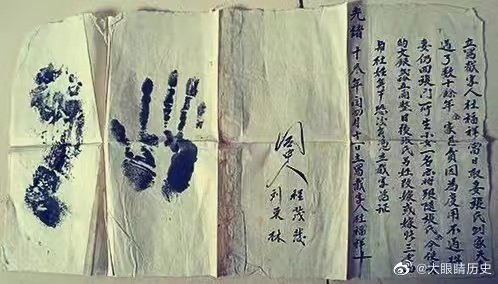
\includegraphics[height=0.36\textwidth,width=0.56\textwidth,viewport=0 0 375 240,clip]{Hand_and_foot-print.png}
\caption*{\hei 微博网页提供的清代光绪十八年~(公元1892年)~的休书}
\label{Collect_Liu_Wu}
\end{figure}
\includegraphics{.jpeg}

立写截字人杜福祥
当日娶妻张氏到家,夫妻过了数十余年。余家甚贫,因为度用不过,将妻仍回张门,所生小女一名,亦将跟随张氏。余今休妻的(得)文银贰拾伍两整,日后张氏另姓改嫁,或嫁张三、李四,与杜姓无干。恐说无凭,立截字为证。

\begin{flushright}
光绪十八年~闰四月十一日~立写截字人~~杜福祥 ~~(画 ``十字押'') ~~~\\

\large{同中人~程茂发、刘秉林} ~~~~~~~~~~~~~~~ \\

\huge{手模}、\huge{足印} ~~~~~~~~~~~
\end{flushright}

\newpage
\hypertarget{ux6253ux9c7cux6740ux5bb6-ux4e4b-ux8427ux6069}{%
\subsection{\texorpdfstring{打鱼杀家\protect\hyperlink{fn514}{\textsuperscript{514}}
之
萧恩}{打鱼杀家514 之 萧恩}}\label{ux6253ux9c7cux6740ux5bb6-ux4e4b-ux8427ux6069}}

\textbf{{[}第一场{]}}

\textbf{开船呐!}

\textbf{儿啊------}

\textbf{【西皮摇板】父女打鱼在河下,家贫哪怕人笑咱。拉住篷索父把网撒,}

\textbf{【西皮散板】年纪衰迈气力不佳。}

\textbf{唉,本当不做这河下生意,你我父女何以度日呀?}

\textbf{儿啊,不要啼哭,将船湾在柳荫之下,凉爽凉爽。}

\textbf{儿啊,将几尾鲜鱼烹煮好了,少时为父还要饮酒。}

\textbf{有人唤我。}

\textbf{是哪一位?}

\textbf{哦,原来是李贤弟。}

\textbf{敢莫要到舟中走走?}

\textbf{待我搭了扶手。}

\textbf{此位是------?}

\textbf{(惊介)这做什么?}

\textbf{老了,不中用了。}

\textbf{儿啊,出舱来见过二位叔父。}

\textbf{小女桂英。}

\textbf{一十六岁,痴长啊。}

\textbf{且慢,方才打得几尾鲜鱼,就在船头之上,你我弟兄畅快饮一回。}

\textbf{儿啊,看酒来。}

\textbf{啊,二位贤弟,愚兄有个酒令儿。}

愚兄做的是河下生意,忌的是``干''、``旱''二字。

不敢说罚,要敬酒三杯。

请------

呃,敬你三杯。

哦,待我看来。

诶!做什么的?

问的是哪一家呀?

你来看,就在前面,八字粉墙,合脊门楼,那就是丁\ldots{}\ldots{}

诶,哼,放肆!

量他也不敢呐。

请------

哦,又有人唤我。

二位贤弟再饮几杯。

哦,原来是丁郎儿,到此何事啊?

你来看,这几日天旱水浅,鱼不上网。改日有了银钱,送上府去。

哦,是是是。

放他去罢,

教他去罢。

(李俊、倪荣 啊,萧兄为何这等\ldots{}\ldots{}。)

他们的人多。

他们的势力大。

这就难讲话了。

本当不做河下生意,怎奈这囊中------唉,惭愧。

哪位贤弟送来?

当面谢过。

有了人家了。

花荣之子,名唤花逢春。

请------

二位贤弟慢走,愚兄不能远送了。

哦,来了。

儿问的是他?

儿啊------

\textbf{【西皮摇板】他本江湖二豪侠,倪荣、李俊就是他。蟒袍、玉带不愿挂,弟兄双双走天涯。}

\textbf{【西皮散板】猛抬头见红日坠落西斜。}

\textbf{儿啊,天色不早,我们回去了吧。}

\textbf{正是:(念)父女打鱼在江下,}

\textbf{(念)堪堪不觉红日落,}

{[}第二场{]}

\textbf{【西皮快三眼】昨夜晚吃酒醉和衣而卧,稼场鸡惊醒了梦里南柯。二贤弟在河下相劝与我,他教我把打鱼的事啊一旦丢却。我本当不打鱼啊关门闲坐,怎奈我家贫穷无计奈何。清早起开柴扉乌鸦叫过,飞过来叫过去【转西皮二六】却是为何。将身儿来至在草堂内坐,桂英儿取茶来为父解渴。}

\textbf{不教儿渔家打扮,怎么偏偏要渔家打扮?}

\textbf{呃------不听父言,就为不孝哇。}

\textbf{这便才是!}

\textbf{是哪个?}

\textbf{你们是哪里来的?}

\textbf{哦,原来是丁府上的教师爷。}

\textbf{哼!}

\textbf{做什么来了?}

\textbf{这几日天旱水浅,鱼不上网。改日有钱,送上府去,何必你来!}

\textbf{旁人来了无有,教师爷你来了么,}

\textbf{哼哼,越发的无有了!}

\textbf{朝廷王法,要它何用?}

\textbf{哼!}

\textbf{哼,尔要锁?}

\textbf{当真要锁?}

\textbf{果然要锁?}

\textbf{如此你就------锁!}

\textbf{不教锁。}

\textbf{哼!}

\textbf{话么,倒是两句好话呀,可惜呀可惜,}

\textbf{可惜你二大爷无有工夫啊。}

\textbf{尔要讲打?}

\textbf{诶呀!老汉幼年间,听说打架,如同小孩子穿新鞋、过新年的一般;如今呐------老了,打不动了啊!}

\textbf{尔当真要打?}

\textbf{果然要打?!}

\textbf{娃娃!待老汉将衣帽留在家中,打个样儿与你们见识见识。}

\textbf{【西皮导板】听一言不由我七窍冒火,}

\textbf{【西皮摇板】不由我年迈人咬碎牙车}\protect\hyperlink{fn515}{\textsuperscript{515}}\textbf{。江湖上叫萧恩不才是我,}

\textbf{【西皮摇板】大战场、小战场见过许多。爷本是出山虎独自一个,}

\textbf{【西皮摇板】尔好比看家犬一群一窝。你本是奴下奴敢来欺我。}

\textbf{慢说是三``羊头'',就是尔这三``狗头'',二大爷何惧!}

\textbf{你是丁府上的教师爷?}

\textbf{你好本领呐!老汉要领教领教。}

\textbf{一定要领教。}

\textbf{这是大十八般武艺?}

\textbf{这小十八样兵器?}

\textbf{这拳脚是?}

\textbf{软硬功夫?}

\textbf{呃,这叫什么?}

\textbf{不好哇。}

\textbf{这叫什么?}

\textbf{呃,不好。}

\textbf{呃,越发的不好啊。}

\textbf{方才撞了老汉三``羊头'',如今我要打你三拳头,放你过去。}

\textbf{哪里有功夫。}

\textbf{着打!}

\textbf{着打!}

\textbf{打得好,只恐打出祸来了!}

\textbf{那贼回去,定不甘休。待为父赶至县衙,抢他一个原告!}

\textbf{不要儿管,取为父的衣帽过来。}

\textbf{好好看守门户,为父去去就来。}\protect\hyperlink{fn516}{\textsuperscript{516}}

{[}第三场{]}

\textbf{(萧桂英
【西皮散板】老爹爹清晨出前去出首,)}\protect\hyperlink{fn517}{\textsuperscript{517}}

\textbf{(众 (内)一十!)}

\textbf{(萧桂英 【西皮散板】倒叫我桂英儿挂在心头。)}

\textbf{(众 (内)二十!)}

\textbf{(萧桂英 【西皮散板】将身儿来至在草堂门口,)}

\textbf{(众 (内)三十!)}

\textbf{(萧桂英 【西皮散板】只等得爹爹回细问根由。)}

\textbf{(众 (内)四十打完!)}

\textbf{(吕子秋 (内)赶下堂去!)}

\textbf{好贼!}

\textbf{【西皮散板】恼恨那吕子秋为官不正,仗势力欺压我受苦的良民呐。上堂来他那里一言不问,责打我四十板呐赶出了头门。}

\textbf{【西皮散板】我这里咬牙关忙往家奔,叫一声桂英儿你快来开门呐。}

\textbf{为父上得堂去,那贼一言不问,将为父重责。}

\textbf{这还不算受屈。他教为父连夜过江与那老贼赔礼,那才算受屈呢。}

\textbf{哎呀------我恨不得飞过江去,我就杀\ldots{}\ldots{}}

\textbf{我要杀贼的满门,方消我心头之恨!}

\textbf{小小年纪,懂得什么?!不用多管,取为父衣帽、戒刀过来。}

\textbf{不用儿管,快些取来。}

\textbf{为父去也。}

\textbf{何事?}

\textbf{小小年纪,去之无益。}

\textbf{有此胆量?}

\textbf{快将儿的衣服、兵刃收拾好了。}

\textbf{壮胆量也是好的。}

\textbf{走哇\ldots{}\ldots{}}

\textbf{做什么?}

\textbf{这门么,关也罢,不关也罢呀。}

\textbf{又做什么?}

\textbf{唉!门都不要了,还要什么家具呀?}

\textbf{唉,不明白的冤家呀,呃\ldots{}\ldots{}(哭介)}

\textbf{不要啼哭,随为父的走哇。}

\textbf{儿啊,此番前去,教儿骂,儿就骂,教儿杀,儿就杀,不要害怕。}

\textbf{走哇。}

\textbf{儿啊,夜晚行船,比不得白日,儿要掌稳了舵!}

\textbf{【西皮快板】这件事不由我心头冒火,今夜晚过江去将他杀却。恨不得插双翅江河越过,}

\textbf{【西皮散板】我的儿因何故放了篷索。}

\textbf{杀人还有什么假的不成?}

\textbf{呀呸!为父在家中不教儿前来,儿是偏偏地要来。这船行半江之中,儿又要回去------也罢!待为父拨转船头,送儿回去。}

\textbf{\textless{}哭头\textgreater{}啊,桂英,我的儿呀!}

\textbf{少时还在此处上船,儿记下了?}

\textbf{儿啊,庆顶珠}\protect\hyperlink{fn518}{\textsuperscript{518}}\textbf{可在身旁?}

\textbf{此番前去,倘有不测,儿自带庆顶珠逃往花家去吧。}

\textbf{我么------儿就不用管了哇。}

\textbf{不要啼哭,随我走哇。}

\textbf{来此已是。}

\textbf{且慢。}

\textbf{收拾好了。}

\textbf{有人么?走出一个来呀。}

\textbf{过府赔罪来了。}

\textbf{哼!}

\textbf{请了。}

\textbf{我来问你:这鱼税银子,可有圣上旨意?}

\textbf{户部公文?}

\textbf{凭着何来?}

\textbf{敢是那吕子秋?!}

\textbf{哼!}

\textbf{【西皮摇板】这税银我不纳是我的本分,你不该差人役打上我门。}

\textbf{儿啊,骂呀!}

\textbf{且慢,我父女有好心献上。}

\textbf{打鱼之时,得来一宗宝贝,名唤庆顶珠。}

\textbf{这\ldots{}\ldots{}耳目甚多。}

\textbf{看刀!}

\textbf{儿啊,随为父的杀呀!}

\newpage
\hypertarget{ux7843ux7802ux75e3-ux4e4b-ux97e9ux5ef7ux51e4ux8c2dux6d3e}{%
\subsection{硃砂痣 之
韩廷凤(谭派)}\label{ux7843ux7802ux75e3-ux4e4b-ux97e9ux5ef7ux51e4ux8c2dux6d3e}}

\textbf{{[}第一场{]}}

\textbf{唉!}

\textbf{【二黄摇板】为续弦前后厅灯光明亮,梦不想今夜晚再做新郎。}

\textbf{抬上堂来(或:}搭上堂来)\protect\hyperlink{fn519}{\textsuperscript{519}}\textbf{。}

\textbf{每人赏银二分(或:}每人赏钱四个)\textbf{。}

\textbf{带他们下面用饭。}

\textbf{待我观看一回。}

\textbf{【二黄慢板】我这里借灯光用目观望,我看她(或:只见她)与前妻一样风光。}

\textbf{【二黄慢板】为什么(或:因何故)皱眉间泪带面上(或:泪带脸上),莫不是嫌年迈难配鸾凰。}

\textbf{【二黄慢板】要穿衣锦绣衫任你选样,}

\textbf{【二黄慢板】要用饭现有那谷米陈仓。}

\textbf{【二黄慢板】这不是那不是难以猜想,尊娘行(或:问娘行)因何事珠泪汪汪,为的是哪桩,你何妨(或:又何妨)细说端详?}

\textbf{【二黄摇板】听她言这婚姻(或:好一似)冰结霜降,一时里惹动我烦恼愁肠。看起来断不可此事勾当,自情愿伴孤灯独守空房。}

\textbf{韩福过来。}

\textbf{命你同媒婆送这位大娘子回去,对他丈夫言讲(或:与他丈夫言讲):前番(那)一百两银子不要,再送他一百两银子,教他好好将养疾病,将大娘子送回,成全他夫妻恩义。就此去罢。}

\textbf{啊大娘子,还有这婚书呢。}

\textbf{唉,就在灯前焚化了罢。}

\textbf{【二黄摇板】伊言道她丈夫病卧床上,没奈何卖妻子暂度时光。将自己比旁人俱是(或:皆是)一样,我岂肯拆散他恩爱鸳鸯。(或:善与恶自有那天理昭彰。)}

\textbf{{[}第二场{]}}

\textbf{【二黄摇板}\protect\hyperlink{fn520}{\textsuperscript{520}}\textbf{】想当年为太守何等荣耀,遇兵荒妻和子无有下梢。多亏了陈太尉将我来保,才能得归田园自在逍遥。}

\textbf{【二黄摇板】忙迫中呃挽定了把礼还到,一时里好教我难解根苗。}

\textbf{呜,你不是昨晚送回去的大娘子么?}

\textbf{既然将你送回,你又来则甚呐?}

\textbf{哦,(原来是)吴相公来了。}

\textbf{哎呀,请坐请坐。}

\textbf{呃,还有话讲啊。}

\textbf{(有话叙谈,}哪有不坐之理,请坐请坐。\textbf{)}

\textbf{啊大娘子,你也坐下。}

\textbf{啊吴相公,昨日听得大娘子说到家中一番苦楚,甚是凄惨。相公有恙在身,改日再来叙谈,为何带病前来?(或:大相公,昨日听得大娘子说到家中一番苦楚。相公你有病在床,病体好了,再来不迟。)}

\textbf{哦,你见了银子,出了一身的通汗,这病就好了么?}

\textbf{哎呀呀,吴相公啊,看将起来,这银子啊,是好物件!}

\textbf{【二黄碰板垛板】我救你的急,救你的难,救你的贫困;全尔的节,全尔的义,全尔的婚呐姻。纵有妻不生子前生造定,我岂肯拆婚姻}\protect\hyperlink{fn521}{\textsuperscript{521}}\textbf{落下了骂名。}

\textbf{啊,啊,呵呵呵哈哈哈\ldots{}\ldots{}(笑介)}

\textbf{请坐请坐。}

\textbf{哎呀呀吴相公啊,我当日也是恩爱夫妻,只因兵荒马乱,中途失散,却无子嗣。若有一子传宗接代,我也就不续弦再娶的了哇。}

\textbf{这\ldots{}\ldots{}子孙前世所修,再续么,也就不必了。(或:}子孙之事,前生所修。再娶么,唉,也就不必了。\textbf{)}

\textbf{言得极是,只是本处孩儿多有不便呐。}

\textbf{本当如此,奈无机会。}

\textbf{这只好凭天机、遇时宜了。}

\textbf{吴相公慢些走啊!}

\textbf{【二黄摇板】他夫妻进门来双双拜倒(或:双双跪倒),口声声叫恩人泪似呃雨抛。非是我用银钱假意行好哇,韩廷凤全仁义一片心苗。}

\textbf{{[}第三场{]}}

\textbf{【四平调】叹光阴去不归无限烦闷,不觉已老两鬓如银。读古书难解我心头烦闷,饮香醪怎畅我衷肠凄清。}

\textbf{哦,你是吴相公,呃,请坐请坐。}

\textbf{你往成都收取账目,呃,必定是发了财了哇。(或:}闻你往成都,收取账目,一定发财的了。\textbf{)}

\textbf{请便。}

\textbf{哦,这是何人?}

\textbf{哦,罢了(罢了),一旁坐下。}

\textbf{呃,不妨不妨,只管地坐下。}

\textbf{呵呵呵哈哈哈\ldots{}\ldots{}(笑介)}

\textbf{啊吴相公,你看这小小的孩童,呃,也(很)知大体呀。}

\textbf{是啊,小孩子原要(他)爹娘教导哇。}

\textbf{啊吴相公,你买他前来,还是为子啊,还是为仆呢?}

\textbf{哦,这等说来(或:}如此说来)\textbf{,是送与我的?}

\textbf{哎呀呀吴相公啊,你真是(或:}你真乃)\textbf{信实人也。}

\textbf{【四平调】吴官人你真真言而有信,你与我谋后代不惜辛勤。感谢你这好意情深义尽,\textless{}行弦\textgreater{}}

\textbf{吴大哥,你请来上坐。(或:}这边坐,这边坐。\textbf{)}

\textbf{请坐,请坐。}

\textbf{【四平调】退一日自当另有条陈。}

\textbf{呵呵哈哈哈\ldots{}\ldots{}(笑介)}

\textbf{哎呀吴官人呐,我如今有了儿子就不愁了。}

\textbf{是啊,吴官人离家日久,我也不便相留(或:}不便强留\textbf{),改日我父子要登门叩谢。}

\textbf{儿啊,送过你吴大爷。}

\textbf{(啊,吴官人何事?)}

\textbf{请来吃酒,请来吃酒。}

\textbf{啊\ldots{}\ldots{}呃,吴官人,请转请转。}

\textbf{改日我父子,呃,要登门再谢。}

\textbf{呃一定要去,一定要去。}

\textbf{啊\ldots{}\ldots{}呃,无有了,请便请便。(或:}吴官人,请呐请呐。\textbf{)}

\textbf{哦------哈哈哈\ldots{}\ldots{}(笑介)}

\textbf{儿啊,随为父的进来。}

\textbf{一旁坐下,待我细看一回(或:待我}细观一回\textbf{)。}

\textbf{【二黄原板】我的儿须从容端然坐定,看形象并非是平等之人。细观他各部位五官端正,这两鬓齐开朗目秀眉清。儿在家可读过圣贤书本,一一地对为父细说分明。}

\textbf{【二黄原板】他说话有分寸智慧聪明,倒像个宦门后不差毫分。可记得是何年月日生辰,说出来将八字细与儿评。}

\textbf{【二黄原板】这小娃言语中隐藏暗景,再问他亲父母便知真情。儿父母年多少在不在,因何故图银钱卖与他人。}

\textbf{儿今年多大年纪了(或:}儿今年几岁了\textbf{) ?}

\textbf{儿父?}

\textbf{死了五载。}

\textbf{儿母?}

\textbf{七旬有余。}

\textbf{(惊介)儿有一十三岁(或:}儿才一十三岁\textbf{)。}

\textbf{(惊介)嗯\ldots{}\ldots{}}

\textbf{【二黄原板】这其间又盘出}\protect\hyperlink{fn522}{\textsuperscript{522}}\textbf{奇情种种,哪有个花甲年又产娇生。}

\textbf{儿啊------}

\textbf{【二黄原板】必然是那老娘将儿蒙混,这内中另有个生儿的娘亲。}

\textbf{哦,儿是捡来的么?}

\textbf{【二黄原板】细盘问这来由日月推论,仔细想当年事越加是真:宣和年四月里成都调任,行至在青州府路遇贼兵。亲生儿在娘怀无有踪影,实可怜贤德妻命赴幽冥。}

\textbf{【二黄散板】这形象好一似韩门真种,举动间与老夫骨肉有情。我这里取菱花照照相品呐,}

\textbf{【二黄散板】半像我半像妻不差毫分。}

\textbf{【二黄散板】亲生子再相逢三生有幸,这才是天地意弄假成真。}

\textbf{不对了,不对了!}

\textbf{(韩玉印 怎么不对呢?)}

\textbf{我那亲生的孩儿,落生下来,左足心上有硃砂红痣。你无有,不是我的亲生儿子啊。}

\textbf{怎么,儿也有?}

\textbf{为父的不信呐,待我看来。}

\textbf{(唉,儿啊------)}

\textbf{【二黄散板】你是我亲生的儿呀名唤玉印,遇兵荒遭失散十有二春。盼娇儿盼得我身染重病,盼娇儿盼得我昼夜不宁。盼娇儿啊不做官告归故呃井,喂呀我的儿呀,梦不想天保佑枯木哇逢春。}

\textbf{你母命丧东平,也曾命人搬尸去了\ldots{}\ldots{}哇,呃\ldots{}\ldots{}(哭介)}

\textbf{言得极是,派人接她前来就是。}

\textbf{正是:(念)北转南来西复东,今朝骨肉又重逢。父子再把菱花照,}

\textbf{(儿啊------)}

\textbf{(念)只怕相逢在梦中。}

\textbf{哦,不是做梦?}

\textbf{玉印,我儿,啊------啊------哈哈哈\ldots{}\ldots{}(笑介)}

\textbf{随我来。}

\newpage
\hypertarget{ux96c4ux5ddeux5173}{%
\subsection{雄州关}\label{ux96c4ux5ddeux5173}}

\textbf{{[}第一场{]}}

\textbf{呼延狄 (念)百万熊罴犯中原,}

\textbf{雷洪切 (念)搅乱宋室不安然!}

\textbf{达林呈 (念)渴饮马上刀头血,}

\textbf{季乐芬 (念)嘿!饥饿人头当饭餐!}

\textbf{众 俺------}

\textbf{呼延狄 金邦大将军呼延狄是也!}

\textbf{雷洪切 金邦副将军雷洪切是也!}

\textbf{达林呈 金邦左先锋达林呈是也!}

\textbf{季乐芬 金邦右先锋季乐芬是也!}

\textbf{萨里哈 前营骁骑大将军萨里哈是也!}

\textbf{耶律浑 后营骁骑大将军耶律浑是也!}

\textbf{提尔雄 左营压队大将军提尔雄是也!}

\textbf{虎骨达 右营护卫大将军虎骨达是也!}

\textbf{呼延狄 列位将军请了------}

\textbf{众 请了!}

\textbf{呼延狄
你我奉了狼主之命,随定四太子,领兵夺取宋室天下,兵到即克。也是宋王气数当尽了。}

\textbf{众 着啊!}

\textbf{呼延狄 这些蛮子怎能苦争恶战,这也是我家狼主洪福齐天也!}

\textbf{众
听觱篥}\protect\hyperlink{fn523}{\textsuperscript{523}}\textbf{一声响,太子升帐,你我两厢伺候。请------}

\textbf{金兀朮
\textless{}点绛唇\textgreater{}军营号响}\protect\hyperlink{fn524}{\textsuperscript{524}}\textbf{,威武雄壮;中军帐,排列刀枪,杀气呃------}

\textbf{众 参见殿下!}

\textbf{金兀朮 站立两厢!}

\textbf{金兀朮
(念)杀气腾腾满乾坤,哀声处处震天庭。宋王失政宠奸佞,锦绣江山一旦倾。}

\textbf{金兀朮
孤,北番大金邦女真国老王殿下四太子、昌平王、御营总兵完颜兀朮。今有宋主无道,宠信奸臣。内奸童贯封为广阳王}\protect\hyperlink{fn525}{\textsuperscript{525}}\textbf{之职。是他前者有密书到孤父王驾下,约定我国兴兵夺取他家社稷。有他以为内应,这宋室天下岂不是唾手而得。自兴兵以来,战无不胜,攻无不取。前日又破了潞安州,守将陆登自刎身亡,甚是悲惨。前面乃是雄州关,守将韩世忠。此人乃是忠勇之士,孤家不忍逼迫于他。意欲招他归顺,助孤一臂之力,何愁大事不成。}

\textbf{金兀朮 众番儿!}

\textbf{众 有!}

\textbf{金兀朮 此番兴兵行至雄州关,不可杀掠黎民,违令者斩!}

\textbf{众 啊!}

\textbf{金兀朮 由此发动人马!}

\textbf{{[}第二场{]}}

\textbf{探子 马来。}

\textbf{探子
(念)短甲随身衲袄齐,肩上横担令字旗。年年岁岁领皇赏。一马冲至军队里。}

\textbf{探子
俺,韩元帅麾下能行探子是也。奉了元帅将令,着俺四路哨探。今有圣上差孙浩督兵前来剿灭金邦,已至三山口。不免飞骑报韩元帅知道!就此马上加鞭。}

\textbf{{[}第三场{]}}

\textbf{韩世忠
【西皮三眼】为金兵急得我心神不定,盼救}兵望眼穿昼夜不宁。陆元帅尽了忠自刎丧命,只一子失陷在万马军营。好教人止不住啊【转\textbf{西皮二六}】腮边泪滚,可叹他夫妻们饮恨幽冥。行公文\protect\hyperlink{fn526}{\textsuperscript{526}}求圣上遣将助阵,因何故十数日渺无回音。在二堂思无计心呃中忧闷,我父子只恐怕难退雄兵。

中军 (念)探马如飞急,叩禀元帅知。

中军 启元帅:探马求见。

韩世忠 吩咐开门!

中军 开门!

众 啊!

韩世忠 \textbf{(念)}探马报音信,升帐问分明。

韩世忠 传探马。

中军 元帅有令:探马进见。

探马 报------告进。

探马 帅爷在上,探马叩头。

韩世忠 打听哪路军情,起来快些讲。

探马 啊,帅爷听禀:

探马
(念)一马哨探似流星,朝中差来孙总兵。十万人马到疆界,禀报元帅得知情。

韩世忠 朝中无有什么姓孙的呀!

探马 在元帅帐下当过副将的。

韩世忠 哦------敢是孙浩?!

探马 正是。

韩世忠 赏尔金牌一面,再去打探。

探马 得令!

韩世忠
且住!想那孙浩,在某帐下曾为副将。只因犯我将令,将他捆打,是他逃至京中,投在\textbf{广阳}府内,做了随侍。今番奉旨督兵前来,焉有不接之理。

韩世忠 中军!

中军 有!

韩世忠 传众将进帐。

中军 众将进帐呃!

\textbf{四将} (内)来也!

\textbf{四将}
(念)元帅传军令,将士共趋迎\protect\hyperlink{fn527}{\textsuperscript{527}}。

\textbf{四将} 参见元帅。

韩世忠 众位将军少礼!

\textbf{四将} 啊!

\textbf{四将} 传末将等进帐,有何军情议论?

韩世忠 圣上命孙浩督兵前来,征剿金人,已到三山口。命你等前去迎接。

\textbf{四将} 啊元帅,那孙浩若问:你家元帅为何不来。我等怎样回答?

韩世忠
你等就说:我家元帅因金兵犯境,城内空虚,不敢擅离汛地,故命我等前来迎接。

\textbf{四将} 那孙浩缘何授得此职?

韩世忠 唉!你等不知他的来历,听我令下:

\textbf{韩世忠
【西皮}原板】韩世忠坐宝帐传言发令,叫一声众将官细听详情:那孙浩平日间行为不正,犯军令责罚他不能徇情呃。逃到了京师地\textbf{广阳}府进,童太尉听谗言懵懂圣君。迎接他务须要言语谨慎,

\textbf{韩世忠 【西皮摇板}】防贼子寻仇起暗箭伤人。

\textbf{四将 得令!}

\textbf{四将 【西皮摇板】韩元帅忠义士谁人不敬,何惧那孙浩贼势利小人。}

\textbf{韩世忠
【西皮摇板】大宋朝八代君徽宗失政,贪酒色戮忠良信宠谗臣。恨蔡京与童贯伤害民命,惹得那四路里齐动刀兵。金兀朮领人马抢夺州郡,逼元戎劳将士苦及黎民。众将官退宝帐各归管汛,}

\textbf{韩世忠 【西皮摇板】且等候四将回再定计行。}

\textbf{{[}第四场{]}}

\textbf{孙浩
\textless{}点绛唇\textgreater{}奉旨领雄兵,蟒罗袍,不愧先人;定斩世忠消吾恨,还报他痛打军刑。}

\textbf{孙浩}
(念)\textbf{胸怀巧诈极聪明,不近贵人怎升腾?只道一生空劳力,运至时来命通亨。}

\textbf{孙浩
某,孙浩,塞北人也。昔在韩世忠麾下以为步军,只因不守军规,专意花酒情浓。抢得一有夫之妇作乐,不想韩世忠便要将俺斩首。是俺推在步兵列名身上,彼时将那步兵斩首号令。又道俺带领无方,将俺捆打,削去头领,赶出不用。俺又羞又恼,一怒奔至京中。恰遇童太尉朝罢而归,是俺闯了他的禁道,将我拿到府中拷问。俺将韩世忠打革之事从头诉说一遍,不想童太尉与韩世忠是旧有仇恨,听了此言,便把俺留在府呃中。因俺善于奉承,是他心中欢喜,想要重用于俺。如今金兀朮兴兵犯界,破了无数城池。眼看要到雄州,那韩世忠本章进京,求兵添将。童太尉奏上一本,命俺提兵前来,剿灭番贼。若是得胜,道韩世忠贪生怕死;若是损兵,便道韩世忠按兵不动。慢说是一个韩世忠,就是百个,也教他有死无生。看前面已是三山口,众将,催动人马!}

\textbf{孙浩 【西皮导板】见旌旗空中飘人声喧震,}

\textbf{孙浩
【西皮原板】抖起}了万丈尘沸沸腾腾。曾记得到京都那般光景,岂料我今日里督领雄兵。韩世忠好比那儿童之分,怎知晓暗中刀要你残生。咱料他如南柯梦魂未醒,

\textbf{孙浩 【西皮摇板}】绑云阳一命倾才晓前情。

\textbf{孙浩
前道}\protect\hyperlink{fn528}{\textsuperscript{528}}\textbf{为何不行?}

\textbf{四将 雄州关总戎麾下四营将校迎接总爷。}

\textbf{众 雄州关总戎麾下四营将校迎接总爷。}

\textbf{孙浩 传。}

\textbf{众 传。}

\textbf{四将 雄州关四营将校迎接总爷}

\textbf{孙浩 你家主帅有多大的官儿,怎么不来迎接本镇。}

\textbf{四将
启禀总爷:主帅为金兵临界,关内空虚,不敢擅离汛地,故而命末将等前来迎接总爷。}

\textbf{孙浩
哼------你住了!本镇钦奉圣命,广阳王钧旨,领兵剿贼,你们主帅也不看在眼内,本当将尔等捆打------}

\textbf{四将 总爷开恩。}

\textbf{孙浩 也罢!待本镇破了金兵回来,再与你主帅辩理。}

\textbf{孙浩 来呀,乱棍逐出!}

\textbf{孙浩 催------军!}

\textbf{孙浩
【西皮摇板】定教他主帅们无处逃奔,少不得斩尔等碎尸粉身。叫众将越过了飞龙奇岭,扫灭了番邦贼奏达捷音。}

\textbf{{[}第五场{]}}

\textbf{韩世忠
【西皮摇板】命四将接孙浩渺无音信,倒教我背地里暗自思忖呐。必然他要报那从先的仇恨,可惜我空费了一片精神。}

\textbf{四将 【西皮摇板】贼孙浩忒无礼令人可恨,全不念数年间共事同营。}

\textbf{四将 参见元帅!}

\textbf{韩世忠 你们回来了。}

\textbf{四将 回来了。}

\textbf{韩世忠 迎接孙浩他可曾讲些什么?}

\textbf{四将 末将等奉令迎接孙浩,那厮言道:你家主帅为何不来?}

\textbf{韩世忠 你等怎生回答?}

\textbf{四将
末将言道:金兵临界,城内空虚,不敢擅离汛地,故命我等前来迎接}

\textbf{韩世忠 那厮如何言道?}

\textbf{四将
那厮言道:本镇钦奉圣命,广阳王钧旨,领兵剿贼,你主帅有多大的官儿,不来迎接本镇。本当将尔捆绑------待等破了金兵回来,再与你主帅辩理。说罢此言,呃,将我等乱棍,呵,逐出来了。}

\textbf{韩世忠 小人得志,以致如此。}

\textbf{探子 报!启禀元帅:孙浩越过飞龙岭,迎战金兵去了。}

\textbf{韩世忠 再探!}

\textbf{韩世忠
且住!我想孙浩越过飞龙岭与金兵迎战,倘有差池本帅难逃罪责。}

\textbf{韩世忠 来,传彦直进帐。}

\textbf{中军 有请少将军。}

\textbf{韩彦直 来也!}

\textbf{韩彦直 (念)战国英雄数伍员,一忿扫平楚国兵。}

\textbf{韩彦直 参见父帅。}

\textbf{韩世忠 罢了!坐下。}

\textbf{韩彦直 谢座。唤孩儿进帐,有何吩咐?}

\textbf{韩世忠
圣上命孙浩督兵前来,征剿金人,那贼从飞龙岭迎敌去了。命你带领人马,暗地保护,需要小心在意,听为父令下:}

\textbf{韩世忠
【西皮摇板】广阳王点孙浩身当重任,命四将迎接他赶回州城。我的儿领人马暗地接应,钦命官须保护谨慎小心。}

\textbf{韩彦直 得令!}

\textbf{韩彦直
【西皮摇板】在帐中领将令怎敢迟顿,暗地里保孙浩谨慎殷勤。}\protect\hyperlink{fn529}{\textsuperscript{529}}

\textbf{韩世忠 众将官,随本帅披挂,催动人马,起兵前往!}

\textbf{{[}第六场{]}}

\textbf{金兀朮 马前来的将官,可是韩元帅?}

\textbf{孙浩 逆贼,俺乃童太尉府中的心腹之人,剿贼大将军孙浩是也!}

\textbf{金兀朮 奸贼一党,休要放走之呃!}

\textbf{{[}第七场{]}}

\textbf{韩彦直
(念)头戴束发紫金冠,金锁铠甲扣连环。胸怀重瞳英雄胆,宝剑出鞘血未干。}

\textbf{韩彦直 俺,韩彦直。奉了父帅之命,暗地保护孙浩。}

\textbf{韩彦直 众将官!}

\textbf{众 有!}

\textbf{韩彦直 杀上前去!}

\textbf{{[}第八场{]}}

\textbf{探子 启元帅:孙浩落马;少爷杀进番营去了!}

\textbf{韩世忠 再探!}

\textbf{韩世忠 且住!孙浩落马,我儿杀进番营,这还了得!}

\textbf{韩世忠 众将官,}

\textbf{众 有!}

\textbf{韩世忠 奋勇当先!}

\textbf{{[}第九场{]}}

\textbf{金兀朮
住了,你这小儿,二次杀进番营,倒有些胆量,饶尔不死,通名上来!}

\textbf{韩彦直 听者:俺乃雄州关总戎之子韩彦直是也。}

\textbf{金兀朮 你就是韩世忠之子么?!}

\textbf{韩彦直 然也。}

\textbf{金兀朮 哎,真乃是将门之子!}

\textbf{韩彦直 呔,番贼通名受死。}

\textbf{金兀朮 孤乃大金邦四太子昌平王兀朮是也。}

\textbf{韩彦直 着打!}

\textbf{韩世忠 彦直,孙浩何在?}

\textbf{韩彦直 被番兵踹为肉泥。}

\textbf{韩世忠 好哇!儿啊,下马来,为父有话言讲。}

\textbf{韩彦直 是。}

\textbf{韩世忠 好奴才!}

\textbf{韩世忠
【西皮散板】为父怎样将儿命,断送孙浩丧番营。金枪刺儿咽喉哽,}

\textbf{韩彦直 【西皮散板】要杀孩儿为何情?}

\textbf{韩世忠
大胆畜生,为父可曾}\protect\hyperlink{fn530}{\textsuperscript{530}}\textbf{吩咐与你?!那孙浩乃是圣上差来,又是广阳王的保举,教儿小心暗护,竟被番营杀死,倘若圣上闻知,必道为父有按兵不动之罪。哎呀!儿啊!岂不把为父的送在枉死城去?!}

\textbf{韩彦直
哎呀,爹爹呀!孩儿奉命暗护孙浩,杀进番营,并无此人。况且儿又不认识于他。}

\textbf{韩世忠 住了!那孙浩乃是领兵元戎,必有旗号,儿也不认得吗?}

\textbf{韩彦直
哎呀,爹爹呀!孩儿虽然奉令暗护孙浩,但是万马营中,犹如刀山剑岭,难道教儿束手待死不成?!}

\textbf{四将 元帅,公子之言甚是,还望元帅开恩。}

\textbf{韩世忠
也罢,命儿三次杀进番营,杀退番邦便罢,如若不然,定斩尔的首级。}

\textbf{韩彦直 得令呐!呵\ldots{}\ldots{}(哭介)}

\textbf{韩世忠 哼!}

\textbf{韩世忠 众将官,直踹番营!}

\textbf{{[}第十场{]}}

\textbf{金兀朮 呔,马前来的敢是韩元帅?}

\textbf{韩世忠 然。马前搭话敢是兀朮?}

\textbf{金兀朮 然。}

\textbf{韩世忠
兀朮!吾主有何亏负尔等,既破潞安州,又来兵犯吾郡,是何理也?}

\textbf{金兀朮
韩元帅,你且停战马,听某一言告禀:你主贪淫失政,宠信奸佞,忠良遭戮,以致刀兵四起。莫若归顺我邦,得了宋室天下,定是三台鼎鼐之位。元帅上察!}

\textbf{韩世忠
兀朮,你韩元帅兵虽少个个勇。你强夺州郡}\protect\hyperlink{fn531}{\textsuperscript{531}}\textbf{,伤害人民,恨不得食尔之肉,还敢多言么?}

\textbf{韩世忠
【西皮摇板】战鼓嗵嗵山岳动}\protect\hyperlink{fn532}{\textsuperscript{532}}\textbf{,番邦贼寇敢逞能。扫灭狼烟归大宋,方显男儿是英雄。}

\textbf{金兀朮 韩元帅。}

\textbf{金兀朮
【西皮摇板】久闻世忠武艺灵}\protect\hyperlink{fn533}{\textsuperscript{533}}\textbf{,今日见面果俊英。堂堂仪表非俗品,胜似战国楚伍员。}

\textbf{金兀朮 韩元帅。}

\textbf{金兀朮 【西皮摇板】你若马前来归顺,孤家与你皇兄称。}

\textbf{韩世忠 住了!}

\textbf{韩世忠
【西皮摇板】兀朮开言真堪恨,气得本帅怒上升。收兵回马保众命,不然杀尔草寇平。}

\textbf{{[}第十一场{]}}

\textbf{韩世忠 参见圣上!}

\textbf{童贯
韩世忠!按兵不动,陷害朝廷命官,有降顺金邦之意!来啊!打入囚车!}

\textbf{韩世忠 唉呀!}

\textbf{探子 报!金兵四面围困。}

\textbf{童贯 再探!}

\textbf{童贯 唉呀!}

\textbf{童贯 也罢!韩世忠,命你杀退金兵,将功折罪呀!}

\textbf{韩世忠 奋勇当先!}

\textbf{金兀朮 好小子呃!}

\textbf{韩世忠 追呃!}

\textbf{韩世忠 哈哈,哈哈,啊------呵呵哈哈哈\ldots{}\ldots{}(笑介)}

\textbf{韩世忠 收兵呐!}

\newpage
\hypertarget{ux9547ux6f6dux5dde-ux4e4b-ux5cb3ux98deux6768ux749f}{%
\subsection{镇潭州 之
岳飞、杨璟}\label{ux9547ux6f6dux5dde-ux4e4b-ux5cb3ux98deux6768ux749f}}

\textbf{{[}第一场{]}}

\textbf{岳飞
\textless{}点绛唇\textgreater{}报国精忠,虎啸龙吟;迎二圣,扫荡烟尘,保主锦绣春。}

\textbf{岳飞
(念)旌旗招展出禁城,武将心思汗马勋。剖心要尽凌云志,迎回二圣方称心。}

\textbf{岳飞
本帅,姓岳名飞字鹏举,宋室驾前为臣。只因奸佞当道,张邦昌陷二圣于沙漠,坐井观天。是我退归林下;今蒙太后二次诏宣,官拜天下都招讨、兵马大元帅;后宫娘娘恩赐五色锦旗,亲绣``精忠报国''。}

\textbf{岳飞
本帅亲承王命,统领六师,扫荡烟尘,恢复河山。今乃黄道吉日,正好兴兵。众位贤弟!}

\textbf{岳飞 人马可齐?}

\textbf{岳飞 香案伺候!}

\textbf{岳飞
祝告:(念)山川社稷、万里旗纛尊神:信官岳飞,今奉圣命,扫荡九龙山杨再兴、长沙王罗延庆、洞庭湖水贼杨幺等。但愿此行,旗开得胜!}\protect\hyperlink{fn534}{\textsuperscript{534}}

\textbf{岳飞 打道出府。}\protect\hyperlink{fn535}{\textsuperscript{535}}

\textbf{岳飞 牛皋听令。}

\textbf{岳飞 命你去到潭州晓谕节度使,命他高垒城郭,本帅大兵随后就到。}

\textbf{岳飞 转来。}

\textbf{岳飞 岳云听令。}

\textbf{岳飞 解押粮草}

\textbf{岳飞 张宪听令。}

\textbf{岳飞 催运粮草}

\textbf{岳飞} 张保\textbf{听令。}

\textbf{岳飞 命你以为总督粮官。}

\textbf{岳飞 吉青听令。}

\textbf{岳飞 随营护卫。}

\textbf{岳飞 施全听令。}

\textbf{岳飞
命你总督三军。}传令下去,众将一路之上,不可马踏青苗,扰害百姓,违令者斩!

\textbf{岳飞} 就此起兵潭州。

\textbf{{[}第二场{]}}

\textbf{岳飞 哦,恩师!}

\textbf{岳飞 不敢,恩师请!}

\textbf{岳飞 门生放肆。}

\textbf{岳飞 门生有何德能,敢劳恩师迎接十里之外?}

\textbf{岳飞 惶恐啊惶恐!}

\textbf{岳飞 我命牛皋前来,为何不见?}

\textbf{岳飞 哦,牛皋至此,未憩鞍马,径自立功去了?}

\textbf{岳飞 嗯------想他此去,必然是大败而归。}

\textbf{岳飞 贤弟,你与敌人交战,胜负如何?}

\textbf{岳飞 怎么样?}

\textbf{岳飞 可曾问过敌人的名姓?}

\textbf{岳飞
呃------你跟随愚兄出兵多年,还是这样粗鲁,倘若得胜而归,教愚兄怎上功劳簿。}

\textbf{岳飞 敢是那杨再兴?}

\textbf{岳飞 此人英勇无敌,你岂是他人对手,待本帅亲自会他。}

\textbf{岳飞
众位贤弟!有所不知,想那杨再兴,乃是将门之子,名门之后,武艺高强,本帅意欲,将他收留帐下,做一膀臂。今日出马,非比寻常,众将只许观阵,不许助战,违令者斩!}

\textbf{岳飞 恩师不必拦阻,待门生先见一阵。}

\textbf{岳飞 就烦恩师谨守城池。}

\textbf{岳飞 众将官,带马迎敌者。}

\textbf{岳飞 杨将军,别来无恙!}

\textbf{岳飞 杨将军,想那年在汴梁小校场,会过一面,难道将军你就忘怀了?}

\textbf{岳飞 然也。}

\textbf{岳飞
杨将军,想你乃是将门之子,忠良之后,因甚事失身落草,岂不玷辱杨氏祖先?听本帅相劝,归顺皇朝,共灭金寇,不失封侯之位,将军三思。}

\textbf{岳飞 住口!好言相劝,执意不听,少时擒在马前,悔之晚矣!}

\textbf{岳飞 决一胜负。}

\textbf{岳飞 这个\ldots{}\ldots{}杨将军,俺若不胜,情愿将潭州奉让。}

\textbf{岳飞
杨将军,你我今日交战,非比寻常,必须一对一个;两下各传将令,众将只许观阵,不许助战,违令者斩。}

\textbf{岳飞 军令不严非为丈夫也。}

\textbf{岳飞 \textless{}叫头\textgreater{}众将官!}

\textbf{岳飞 只许观阵,不许助战,违令者斩!}

\textbf{岳飞 【西皮小导板】叫三军与爷战鼓操,}

\textbf{岳飞
【西皮快板】马前闪出一英豪。杨家世代把国保,因何埋名在山巢。劝你马前归顺好,封妻荫子永在朝。}

(上手(岳飞)大边,一扯两扯,幺二三往外把盖下手(杨再兴)枪左转身(下手右转身)到里边打一个腰封、两个腰封,被往里面盖右转身(下手左转身)到外边,接一个腰封、两个腰封,把盖撤枪,撤右脚斜向上场门,上左脚刺在上场边里面的下手左右两马腿,左刺耳\protect\hyperlink{fn536}{\textsuperscript{536}},被下手盖,撤枪撤左腿在下场门边外面接下手两个刺马腿,盖下手左刺耳,搭、拉归里边面外、下手面里,搭、兜转身过到小边,面对过大边的下手掣肘,撤枪两人对脸左右左三个刺马腿,一二三绕、边绕边走从外面过到大边,一二三绕,边绕边走从外面过到小边,下手向内侧刺上手马腿、上手挑起向里刺肚,从里边左转身到外边向外侧刺下手马腿、下手挑起来刺肚,下手直着过到小边,上手接刺肚向右反转身从里边过到大边,二人合身往里一盖两盖,上手手平伸扎下手一枪左转身(下手左手拿枪滑上手扎出的枪、右转身右手掏翎,送到嘴叼翎,枪交右手),上手左手捋胡子、跨右腿、左转身又扎下手一枪(下手右手枪滑上手枪,右转身左手掏翎子),上手转过来扔胡子、枪收回来平托、左手山膀,大边里边站斜向外亮住(下手转过来右手枪剜萝卜、右手伸出、枪头斜向下,左手拿翎横胸前,弓箭步外边站斜向里亮住)\protect\hyperlink{fn537}{\textsuperscript{537}}

(拉上、斜亮,到台口正亮,一二三夺换位亮,一二三夺分开,一合两合,岳飞归小边,幺二三岳被勾走马腰封到大边、再被一压、被漫头左转身到中间面向里一别(杨同时归中间里面向外一别),岳飞撤枪向里面斜刺、刺空(杨出枪贴岳背扎脖),岳飞左转身用枪杆把杨枪搕出去、捋胡子下,杨望岳捋枪向外望、斜托枪亮住,耍下场追下)\protect\hyperlink{fn538}{\textsuperscript{538}}

\textbf{岳飞 绑了!}

\textbf{{[}第三场{]}}

\textbf{岳飞 杨将军,你我再决胜负。}

\textbf{岳飞 回营!}

\textbf{{[}第四场{]}}

\textbf{岳飞 将岳云绑了上来!}

\textbf{岳飞 小奴才,何人教你出马?何人教你出马?}

\textbf{岳飞
大胆奴才!想那杨再兴,乃是将门之后,为父指望收服于他,作为膀臂。故而不许旁人助战,你众位叔父都不敢违抗为父的将令,惟有你这小畜生,你敢犯我的军规吗?}

\textbf{岳飞 斩!}

\textbf{岳飞 众位贤弟,敢是与奴才讲情?}

\textbf{岳飞 可知本帅令出山岳动,这言发------神鬼惊!}

\textbf{岳飞 斩!}

\textbf{岳飞 \textless{}叫头\textgreater{}岳云,奴才!}

\textbf{岳飞 怎么你要回去见你那祖母、娘亲么?}

\textbf{岳飞 掌起面来!}

\textbf{岳飞 \textless{}三叫头\textgreater{}岳云,娇儿,唉,儿啊!}

\textbf{岳飞 为父今日要将儿斩首,怎么你要回去见你那祖母、娘亲么?}

\textbf{岳飞 嗯,只怕儿今生今世就不能相见了。}

\textbf{岳飞 斩!}

\textbf{岳飞 赦了。}

\textbf{岳飞 将岳云带了上来!}

\textbf{岳飞
奴才,本当将你斩首,念在你众位叔父苦苦讲情,死罪已免,活罪难容。}

\textbf{岳飞 牢子手,将奴才重责四十!}

\textbf{岳飞} 张保\textbf{听令!}

\textbf{岳飞
命你押解岳云,去到杨再兴营盘,对他言讲:岳云解粮在先,本帅传令在后,不知有此军令,在阵前冒犯将军,回营就要斩首;多亏满营将官讲情,死罪已免,活罪难容,重责四十,请将军验伤。上覆杨将军,明日还在阵前相会。掩门!}

\textbf{{[}第五场{]}}

\textbf{杨璟 (念)生前为大将,死后做忠魂。}

\textbf{杨璟
吾乃杨璟阴魂是也。今有孙男再兴,落草为寇。岳元帅难以收服,我不免去至宋营,梦中授他撒手金锏,助他成功。}

\textbf{杨璟 鬼卒,宋营去者。}

\textbf{杨璟
【二黄原板】我杨家祖居在梅花山后,老王爷锤换带才把宋投。都只为再兴儿落草为寇,岳元帅无良谋难把他收。教鬼卒前引路宋营来走,见了那岳元帅细}说从头。

\textbf{{[}第六场{]}}

\textbf{岳飞
【二黄原板】清晨起打一仗龙争虎斗,战不过杨再兴脸面惭羞。在虎帐传一令严加防守,迎二圣我才得展放眉头。}

\textbf{杨璟 【二黄摇板】听谯楼打罢了三更时候,到宋营见元帅细说根由。}

\textbf{岳飞 请问老先生尊姓大名,家住哪里,来到我营有何贵干?}

\textbf{杨璟 老夫祖居磁州梅花山后,杨璟是也。}

\textbf{岳飞 哦,原来是前辈老先生,失敬了。老先生有何见谕?}

\textbf{岳飞 元帅受我一礼。}

\textbf{岳飞 老先生施礼为何?}

\textbf{杨璟 只因孙儿再兴,不幸失身落草,还望元帅加以收服。}

\textbf{岳飞 本帅倒有此意,怎奈再兴武艺高强,难以收服。}

\textbf{杨璟 杨家梅花枪暗藏撒手锏,待老夫传授与你。}

\textbf{岳飞 领教了!}

\textbf{杨璟 【二黄摇板】我杨家梅花枪暗藏撒手,}

\textbf{岳飞 【二黄摇板】老先生秉忠心万古名留。}

\textbf{杨璟 【二黄摇板】但愿得收服他鞍前马后,}

\textbf{岳飞 【二黄摇板】他本是将门子啊必定封侯。}

\textbf{杨璟 【二黄摇板】哗喇喇打开了玲珑甲胄,}

\textbf{(众 \ldots{}\ldots{}醒来。)}

\textbf{岳飞 【二黄散板】多蒙你进帐来枪锏传授。猛然间又只见红日当头。}

\textbf{(报子 再兴讨战。)}

\textbf{岳飞 带马阵前去者。}

\textbf{岳飞 杨将军,昨日小儿阵前多有冒犯!}

\textbf{岳飞 岂敢。你我今日再决胜负。}

\textbf{岳飞 话出不悔,真丈夫也。放马过来。}

\textbf{(岳飞、杨再兴开打)}

\textbf{岳飞 杨将军,本帅失手了。}

\textbf{岳飞 弃暗投明,真乃俊杰也。欲与将军结为金兰,万勿见却?}

\textbf{岳飞 不必推辞,你我望空一拜。}

\textbf{岳飞 不必查点,兵合一处。}

\textbf{岳飞 众将官,同进潭州!}

\newpage
\hypertarget{ux516bux5927ux9524}{%
\subsection{八大锤}\label{ux516bux5927ux9524}}

\textbf{{[}第一场{]}}

\textbf{(【撤锣】【帽子头】王佐上)}

\textbf{王佐 (念)若为(或:欲为)天下奇男子,须立人间未有功。}

\textbf{探子 陆文龙讨战。}

\textbf{岳飞 再探!}

\textbf{探子 得令!}

\textbf{岳飞
\textless{}叫头\textgreater{}天呐,天!番邦出了陆文龙,此乃------天亡宋也。}

\textbf{王佐 啊元帅,想那陆文龙,敢莫是当年潞安州节度使陆登之子么?}

\textbf{岳飞 正是。}

\textbf{王佐 闻得他父命丧金人之手,如今为何反助仇人?}

\textbf{岳飞
贤弟哪里知道,当初金兵大破潞安州,此子未满三月,他怎能知晓。}

\textbf{王佐
也罢,待俺王佐,诈降番营。顺说陆文龙来降,不知元帅意下如何?}

岳飞 唉,贤弟,画虎不成反类其犬。哎,你料理军务去吧。

\textbf{王佐 是,告呃退。}

\textbf{岳飞 众将官,小心防守。}

{[}第二场{]}

\textbf{(王佐 唉!)}

\textbf{王佐 【二黄导板】听谯楼打初更玉兔东上,}

\textbf{王佐 【回龙】为国家、秉忠心、食君禄、报王恩,昼夜奔忙。}

\textbf{王佐
【二黄原板】想当年在洞呃庭逍遥放荡,到如今食君禄未报宋王。岳大哥他待我手足一样,我王佐无功劳怎受荣光?今夜晚思一计番营去闯,落一个美名儿万载传扬。}

\textbf{王佐
想}俺(或:想我)王佐,自投宋以来,寸功未立。今日岳元帅杀得大败。俺王佐
若能思得一计,诈降番营,顺说陆文龙来降,岂不是大功一场,名垂千古?

\textbf{王佐
【二黄原板】怎能够今夜晚番营得进,前后话向文龙细说真情(或:衷情)。}

\textbf{王佐 【二黄原板】前也思、后又想无有计定,倒不如上公案细看古今。}

\textbf{王佐 《前唐》?}

\textbf{王佐 不好哇!}

\textbf{王佐 《后汉》!}

\textbf{王佐
呜哙呀!想汉室卫律、苏武,同往北国催贡,一个降顺番邦,一个打入羊群,食
毡饮雪,还是忠心不改,与岳大哥一般无二矣!}

\textbf{王佐
【二黄原板】汉室中(或:汉朝中)卫律声名不正,却为何那苏武一片丹心。饥食毡、渴饮雪忠心耿耿,天保护、地保佑暗有神灵。}

\textbf{王佐 《后汉》?}

\textbf{王佐 不好呃!}

\textbf{王佐 《(东周)列国(志)》。}

\textbf{王佐 还是看看《列国》罢。}

\textbf{王佐 ``要离断臂刺庆忌'',``要离断臂刺庆忌''\ldots{}\ldots{}}

\textbf{王佐
且住,想那要离断臂,刺死公子庆忌,(此)乃大丈夫所为,俺王佐何不学他一学?}

\textbf{王佐
【二黄散板】那要离呀断臂行果有志量(或:颇有志量)呐,留下了美名儿万载传扬。我王佐学断臂番营呐去闯啊,顾不得生和死啊天作主张。}

\textbf{旗牌 (王将军)醒来!)}

\textbf{王佐
【二黄散板】霎时间痛得我神魂不定,好一似滚油煎乱箭攒心。睁开了昏花眼难以扎挣,为国家斩断臂要留美名。}

\textbf{旗牌 将军为何如此?}

\textbf{王佐
尔等不可声张。来来来,这有书信一封,送往大帐(或:送到大帐)岳元帅。就说我,呃,另有公干去了哇。}

\textbf{旗牌 遵命。}

\textbf{王佐 转来。}

\textbf{旗牌 在。}

\textbf{王佐 千万不可走漏风声。}

\textbf{旗牌 遵命。}

\textbf{王佐 且住,趁此天色朦胧,我不免诈降番营去者。}

\textbf{王佐 呼------呜\ldots{}\ldots{}}

{[}第三场{]}

\textbf{旗牌 有请元帅。}

\textbf{岳飞 (念)闷坐大营无良计,愁思昼夜费心机。}

\textbf{岳飞 何事。}

\textbf{旗牌 王将军书信呈上。}

\textbf{岳飞 待我看来。}

\textbf{岳飞 呜哙呀,原来王贤弟诈降番营去了。}

\textbf{岳飞 来,王贵进帐。}

\textbf{王贵 参见元帅。}

\textbf{岳飞 命你巡营瞭哨,待等王佐将军消息。需要小心!}

\textbf{王贵 得令!}

{[}第四场{]}

\textbf{金兀朮 (念)兴兵攻宋室,}

\textbf{陆文龙 (念)一战建奇功。}

\textbf{金兵 启狼主,拿住奸细一名。}

\textbf{金兀朮 押进帐来。}

\textbf{王佐 叩见狼主。}

\textbf{金兀朮 唗!大胆奸细,竟敢前来窥探。来------推出斩了!}

\textbf{王佐 (啊)慢来慢来,留头讲话呀。}

\textbf{陆文龙 啊,是啊,父王要留头讲话。}

\textbf{金兀朮 你且讲来。}

\textbf{王佐
是。难臣王佐,乃岳飞帐下一名随营参军。见他屡次杀得大败,是我劝他归降(或:
归顺);(不想)他是执意不肯。当时拔剑,断臣左臂,言道:誓要扫灭金邦,迎
请二圣还朝,然后再将难臣斩首。哎呀狼主啊!如今,我死又死不了,活是活受
罪呀!唉,狼主救命呐,呃\ldots{}\ldots{}(哭介)}

\textbf{金兀朮 孤家不信,一派谎言。}

\textbf{王佐 现有断臂(在此)为证。}

\textbf{金兀朮 我却不信。}

\textbf{王佐 狼主请看------}

\textbf{金兀朮 呜哙呀,岳飞呀岳飞,降与不降,但凭于你。为何下此毒手?!}

\textbf{金兀朮 罢了,你起来,孤家收留于你也就是了。}

\textbf{王佐 谢狼主!}

\textbf{金兀朮 如今归顺我国,就是我国人了,必须与你改个名字。你叫什么?}

\textbf{陆文龙 是呀,要改个名字的才是。他叫什么?}

\textbf{王佐 唉,苦------哇!呃\ldots{}\ldots{}(哭介)}

\textbf{金兀朮 有了有了,你为孤家吃了苦了。就叫作``苦人儿''罢!}

\textbf{陆文龙 ``苦人儿''------呵,甚好。}

\textbf{王佐 是。}

\textbf{金兀朮 我命太医与你调治伤痕。满营之中,任你闲游。出帐调治去罢。}

\textbf{王佐 是,谢狼主。}

\textbf{王佐 呼------呜\ldots{}\ldots{}}

\textbf{金兀朮 啊,儿啊,}为父已命人去搬取铁浮图,攻打宋营。正是:

\textbf{金兀朮 (念)}恼恨岳飞太不仁,

陆文龙 \textbf{(念)}军中哪有断臂刑!

{[}第五场{]}

\textbf{(乳娘
【二黄摇板】何日里才能得冤冤相报,思想起当年事心似火烧。撇故土到他乡谁为倚靠,屡次里想回国无路可逃。}\protect\hyperlink{fn539}{\textsuperscript{539}}\textbf{)}

\textbf{王佐 走哇!}

\textbf{王佐
【二黄摇板】这几天到番营未有巧机}\protect\hyperlink{fn540}{\textsuperscript{540}}\textbf{,怎能够向他人来把话提(或:细说端的;细说端倪)。}

\textbf{王佐 来此已是陆文龙的营盘,待我来偷觑偷觑。}

\textbf{乳娘 啊------哪里来的奸细,小番,与我拿下了。}

\textbf{王佐
啊老太太,莫要高声呐。(我不是奸细呀,)我就是狼主新收下的一个残废人,
取名``苦人儿'',就是我哇。}

\textbf{乳娘
啊,不错不错。殿下言道,有一南朝将官,名唤王佐,投顺我邦,改名``苦人
儿'',呃,就是足下么?}

\textbf{王佐 正是!}

\textbf{乳娘 哦,我们是幸会呀。}

\textbf{王佐 幸会呀。}

\textbf{王佐 啊老太太,听你讲话,不像此地(或:此处)人氏啊。}

\textbf{乳娘 本不是此地人氏。}

\textbf{王佐 哪里人氏?}

\textbf{乳娘 老身乃是湖广潭州人氏。}

\textbf{王佐 哦,老太太,你是湖广潭州人么?}

\textbf{乳娘 正是。}

\textbf{王佐 呵呵,这倒巧得紧(或:这倒巧得很)呐,我也是湖广潭州人呐。}

\textbf{乳娘 哦,如此说来,我们是同乡?!}

\textbf{王佐 是同乡啊。}

\textbf{(乳娘 重见一礼。)}

\textbf{王佐 好,重见一礼。}

\textbf{乳娘 (念)久旱逢甘雨,}

\textbf{王佐 (念)他乡遇故知。}

\textbf{王佐 啊,老太太你缘何至此?}

\textbf{乳娘
噤声!我与将军乃是同乡,说也无妨:老身薛氏,当年在潞安州陆登陆大老爷府
中,以为乳娘;那年金兵打破城池,老爷、夫人尽忠、尽节而死,撇下未满三
月的陆公子,,被狼主捉回金邦,算来一十六载。唉,陆家的冤仇何日得报哇,
啊,啊\ldots{}\ldots{}(哭介)}

\textbf{(王佐 哦哦哦,是是是\ldots{}\ldots{})}

\textbf{王佐 唉!实实地可怜呐!}

\textbf{乳娘 唉!实实地可怜呐!}

\textbf{王佐 啊老太太,(但不知)那陆公还有后么?}

\textbf{乳娘
怎说无有呃,昨日在两军阵前,连挑宋将数员上将}\protect\hyperlink{fn541}{\textsuperscript{541}}\textbf{,那不就是陆公子么。}

\textbf{王佐 哦?那就是陆公子么?}

\textbf{乳娘 嗯,正是。}

\textbf{王佐 呵呵,我王佐今日来的好机会也!}

\textbf{王佐
【二黄摇板】听罢言来喜心上,尊声安人听端详:我断臂原本为小殿下呀,舍死忘生到番邦。}

\textbf{乳娘 如此说来,呃,你为我家公子吃了苦了哇!}

\textbf{王佐 呜------不妨啊。}

\textbf{王佐
【二黄摇板】这断臂的情由休声嚷啊,泄漏机关祸难当。待等殿下回营帐,全仗安人作主张。}

\textbf{(乳娘
公子已回,快快躲避。}\protect\hyperlink{fn542}{\textsuperscript{542}}\textbf{)}

\textbf{王佐 哦,来了!}

\textbf{王佐 来了。}

\textbf{(陆文龙上)}

\textbf{王佐 ``苦人儿''叩见殿下。}

\textbf{陆文龙 罢了。``苦人儿'',这几日你往哪里去了?}

\textbf{王佐
这几日(或:这些天)被那些平章、将官们,这个请我吃酒,那个叫我(或:请我)
说评书,故而未能前来,与殿下请安(或:与千岁请安)呐。}

\textbf{陆文龙 哦,你还会说评书么?}

\textbf{王佐 呃,我是一肚子的(评)书啊。}

\textbf{陆文龙 你且稍待。乳娘有请!}

\textbf{乳娘 殿下何事?}

\textbf{陆文龙 啊乳娘,有个``苦人儿'',他会说评书。请至出来,一同听书。}

\textbf{乳娘 好好好。}

\textbf{陆文龙 啊``苦人儿'',这就是我家乳娘,上前见过。}

\textbf{王佐 哦,这就是乳娘老太太?}

\textbf{王佐 啊老太太,你好哇。}

\textbf{乳娘 ``苦人儿''你好哇!}

\textbf{陆文龙 呃,你快快说来。}

\textbf{乳娘 啊,殿下,此时要有一个座位。}

\textbf{陆文龙 你坐下说吧。}

\textbf{王佐 呃,慢来慢来,殿下在此,哪有``苦人儿''的座位呀?}

\textbf{陆文龙 咱们师兄弟,您甭客气。}

\textbf{乳娘 我们是自己人,不要客气。坐下罢。}

\textbf{王佐 谢座。}

\textbf{王佐 啊殿下,你是爱听文的呀,还是爱听武的呢?}

\textbf{陆文龙 小王习武,自然是爱听武的。}

\textbf{王佐 哦,武的。}

\textbf{乳娘 自然武的好哇(或:我是爱听武的)。}

\textbf{王佐 是忠的,还是奸的呢?}

\textbf{陆文龙 小王喜的是忠臣,恨的是奸佞。}

\textbf{王佐 哦------爱听忠的。呃,待我来说一段``骅骝思乡''罢。}

\textbf{陆文龙 哦,``骅骝思乡''?嗯,这个故事,呃,倒是要听上一听。}

\textbf{乳娘 是啊,``苦人儿''你且讲来。}

\textbf{(王佐拍醒木)}

\textbf{陆文龙 啊,这做什么?}

\textbf{王佐 这是我们说评书的}规矩呀。

陆文龙 哦,说书的有规矩?那唱戏的就更有规矩了。

\textbf{王佐 是啊,(或:呃,)无有规矩,就不成方圆了。}

\textbf{乳娘 是啊,殿下,无有规矩,就不成方圆了。}

\textbf{陆文龙 哦,这是他们的规矩?}

\textbf{乳娘 是啊。}

\textbf{陆文龙 哎,就依你的``规矩''。}

\textbf{王佐
(念)道德三皇五帝,功名夏后商周;英雄五霸闹春秋,顷刻兴亡过手。}

\textbf{王佐
(念)青史几行名姓,北邙无数荒丘;前人田地后人收,说甚龙争虎斗。}

\textbf{(王佐拍醒木)}

\textbf{陆文龙 哎,他又来了。}

\textbf{王佐
残词道罢(或:残词念罢),书归正传。花开两朵,各表一枝。话表:大宋朝真
宗天子在位,朝中有一家大大的忠良,名唤杨延昭。}

\textbf{(王佐拍醒木)}

\textbf{陆文龙 嗯------杨延昭是个忠良?}

\textbf{乳娘 是啊。(或:忠良事啊。)}

\textbf{王佐
只因北国屡次交战,被那杨元帅杀得大败。那北国萧后就勾通了南朝一个大大
的奸佞(或:一家大大的奸佞),名叫王钦若。}

\textbf{陆文龙 王钦若是个奸佞么?}

\textbf{王佐
嗯,大大的奸佞呐。他与杨家旧有仇恨。一日,真宗早朝,那王钦若出班奏道,说道,北国出了一骑好马,日行千里,夜走八百,名为``日月骕骦马''。}

\textbf{陆文龙 嗯,是一骑好马!}

\textbf{乳娘 嗯,是一骑好马啊。}

\textbf{王佐
那圣上闻奏,就动了爱马之意(或:爱马之心)。问道:命何人前去盗马呀?那王钦若又奏道:非杨延昭不可哇。那圣上(或:宋王)就命杨延昭(前)去盗马。那杨元帅奉旨回来,是闷闷而不乐哇。他帐下有一员虎将,此人姓孟名良字佩仓------}

\textbf{(王佐拍醒木)}

\textbf{陆文龙 啊?}

\textbf{王佐 (呃,这)三关的孟良是哪个(儿)不晓哇?!}

\textbf{乳娘 是啊,三关孟良哪个不晓。}

\textbf{陆文龙 哦,哦------嗯。}

\textbf{王佐
进帐问起情由,当时就讨下了一枝将令。呃,呃,不到一日二啊,二日三,他就混进番营去了。}

\textbf{陆文龙 他是怎样混进去的?}

\textbf{王佐
呃、呃,(呃\ldots{}\ldots{})他会说(或:他能通)三川六国的番语呀。}

\textbf{陆文龙 哦------原来如此。嗯,后来呢?}

\textbf{王佐 嗯,(呃,呃,)不到一月呀,竟将此马盗回来了。}

\textbf{陆文龙 哦------盗回来了?!嗯,此人有能耐。}

\textbf{王佐 不错,有能耐。可惜呀!}

\textbf{陆文龙 可惜什么?}

\textbf{王佐
可惜那马,七日七夜,不食草料,眼望北番,大叫(了)三声,呵嘿,就饿死了。}

\textbf{陆文龙 哦------?这是何意呀?}

\textbf{王佐 呃,不过是思乡罢!}

\textbf{陆文龙 哦,这畜类还会思乡么?}

\textbf{乳娘 啊殿下,畜类会思乡,何况人乎?}

\textbf{王佐 啊老太太,如今的人呐,还不如个畜类呢!}

\textbf{王佐
【二黄摇板】那马倒有思乡意,如今的人儿不如它。父母冤仇全不管(或:父母冤仇抛撇下),反把仇人当自家。}

\textbf{陆文龙 好------}

\textbf{(王佐拍醒木)}

\textbf{王佐 完了。}

\textbf{陆文龙 啊?完了么?}

\textbf{王佐 完了。}

\textbf{陆文龙 哎呀,不热闹哇\ldots{}\ldots{}}

\textbf{王佐
(呵,《八大锤》带``断臂'',还不热闹?)不热闹\ldots{}\ldots{}唉,待我来说一段本朝四狼主,当年大破潞安州的故事罢。}

\textbf{陆文龙 哦?可是我父王?}

\textbf{王佐 正是。}

\textbf{陆文龙 嗯。我倒要听上一听。呵哈,可热闹?}

\textbf{王佐 (哼,)热闹得很呐!}

\textbf{陆文龙 哦,你快些讲来。}

\textbf{王佐
呃------慢来,慢来。我这里有画图一幅,我们挂将起来(或:悬挂起来),照图言讲啊。}

\textbf{陆文龙 挂了起来。}

\textbf{陆文龙
啊------``苦人儿'',这画图之上,有许多的兵将,是金兵还是宋将?}

\textbf{王佐 金兵也有,}宋将也有哇。

\textbf{陆文龙
啊,``苦人儿'',有一员大将,手执宝剑,自刎而死,他是何人?}

\textbf{王佐
(呃,)这就是潞安州节度使,陆登陆老先生。只因我国狼主打破城池,他万般
无奈,拔剑自刎尽忠了。}

\textbf{陆文龙
哦------尽忠了。啊``苦人儿'',那旁有一妇人,悬梁自尽,她是何人?}

\textbf{王佐 这就是陆老夫人。见她丈夫尽忠,她就悬梁自缢,尽节了哇。}

\textbf{陆文龙
哦------尽节了。哦,``苦人儿'',有一员大将,跪在尘埃,好像我父王模样,他是何人?}

\textbf{王佐 (呃,)正是我国四狼主。}

\textbf{陆文龙 哦,是我父王。他为何与他下拜呀?}

\textbf{王佐 我国四狼主念他是个忠良,故(而)与他下拜呀。}

\textbf{陆文龙 哦------我父王拜得,呃,小王也可拜得么?}

\textbf{王佐 (哦,)殿下(要下拜)么?}

\textbf{陆文龙 正是。}

\textbf{王佐 呃呃,正拜,正拜!}

\textbf{陆文龙 啊------陆老先生在上,受小王大礼参拜!}

\textbf{王佐 (啊,)陆老先生,我家殿下拜你,你要明白呀。}

\textbf{陆文龙 啊``苦人儿'',有一妇人,怀抱婴儿,躲在一旁,她是何人?}

\textbf{王佐
这就是陆\ldots{}\ldots{}呃,呃,这就是陆府的乳娘。见她主人一个尽忠,一个尽节,死得可怜,她在一旁落泪呀。}

\textbf{乳娘 呃------呜呜呜\ldots{}\ldots{}(哭介)}

\textbf{陆文龙 啊乳娘,你为何啼哭啊?}

\textbf{乳娘
唉!我见他一家死得可怜,故而------啼哭啊,呜呜呜\ldots{}\ldots{}(哭介)}

\textbf{陆文龙 啊``苦人儿'',我把乳娘好有一比呀。}

\textbf{王佐 比作何来?}

\textbf{陆文龙 看兵书落泪------}

\textbf{王佐 此话怎讲?}

\textbf{陆文龙 替古人担忧哇。}

\textbf{王佐 (啊------)是啊,老太太你可替古人担的什么忧哇?}

\textbf{乳娘 唉!是啊,我替古人担的什么忧。}

\textbf{陆文龙 啊``苦人儿'',他为何立尸不倒?}

\textbf{王佐 若问(他)立尸不倒么?}

\textbf{陆文龙 是啊。}

\textbf{王佐 唉!恐怕他后人,不与他父母报仇,故而立尸不倒。}

\textbf{陆文龙 哦------他还有后人么?}

\textbf{王佐 有道是``忠良不绝后''呃。}

\textbf{乳娘 是啊,忠良不绝后哇。}

\textbf{陆文龙 嗯------此子何在?}

\textbf{王佐 被我国四狼主带回来了。}

\textbf{陆文龙 哦?带回来了------他,他,他今年有多大年纪?}

\textbf{王佐
(呃,他)今年么\ldots{}\ldots{}呃,哦,哦\ldots{}\ldots{}(他今年)一十六岁了哇。}

\textbf{陆文龙 哦,一十六岁?与小王同庚呐。}

\textbf{王佐 哦,殿下也是一十六岁么?}

\textbf{陆文龙 正是。}

\textbf{王佐 呃(或:呵呵),这倒巧得很呐。}

\textbf{陆文龙 嗯------此子本领如何?}

\textbf{王佐 若论他的本领么,嗯------两军阵前,他,他,他能力敌万人!}

\textbf{陆文龙 哦------他、他、他------能力敌万人?}

\textbf{王佐 嗯------}

\textbf{陆文龙
呵,呵,哼------(冷笑介)他既然力敌万人,为何不与他父母报仇?}

\textbf{王佐 唉!不提``报仇''还则罢了,提起``报仇'',令人好恨呐!}

\textbf{陆文龙 恨者何来?}

\textbf{王佐 他非但不替他父母报仇,如今反认仇人为父!}

\textbf{陆文龙 哦------}

\textbf{陆文龙 嗯------他叫什么名字?}

\textbf{王佐 (他叫陆\ldots{}\ldots{})他叫------陆文龙。(低声)}

\textbf{陆文龙 他叫什么名字?}

\textbf{王佐 (他)叫陆文龙。(含糊)}

\textbf{陆文龙 到底叫什么?}

\textbf{王佐 诶------他、他\ldots{}\ldots{}他叫陆文龙啊!}

\textbf{陆文龙 唗!胆大``苦人儿'',戏耍小王,休走,看剑!}

\textbf{乳娘 唉------殿下,这就是你全家遭害的故事。}

\textbf{陆文龙 怎么讲?!}

\textbf{乳娘 遭害的故事呀!}

\textbf{陆文龙 \textless{}双叫头\textgreater{}爹爹,母亲!哎呀------}

\textbf{王佐 (公子)醒来!}

\textbf{陆文龙 【二黄散板】听一言来珠泪掉,}

\textbf{王佐 (公子)醒来!}

\textbf{陆文龙
\textless{}三叫头\textgreater{}爹爹,母亲!唉------爹娘啊\ldots{}\ldots{}(哭介)}

\textbf{陆文龙 【二黄散板】不由小王怒全消。三尺龙泉出了鞘,}

\textbf{王佐 哪里去?}

\textbf{陆文龙 【二黄散板】斩尽金兵回宋朝。}

\textbf{王佐 \textless{}叫头\textgreater{}公子!}

\textbf{王佐 【二黄散板】公子休要(或:公子不必)珠泪掉,快想良谋回南朝。}

\textbf{陆文龙
\textless{}叫头\textgreater{}哎呀叔父啊!那贼见岳元帅闭门不出,明日欲用取铁浮图攻打宋营,如何是好?}

\textbf{王佐
(哎呀!)------有了,待我修下书信一封,公子用箭,射入宋营,教那岳元帅也好作一准备。}

\textbf{陆文龙
待我溶墨。}\protect\hyperlink{fn543}{\textsuperscript{543}}

\textbf{王佐 待我修书。}

\textbf{王佐 公子!}

\textbf{陆文龙 恩公、乳娘,受我一拜!}

\textbf{陆文龙
\textless{}三叫头\textgreater{}爹爹,母亲!唉------我那\ldots{}\ldots{}(哭介)}

\textbf{王佐 噤声!}

\textbf{(陆文龙下)}

\textbf{乳娘 这一下他就明白了。}

\textbf{王佐 他明白了,我也残废了。}


\item
  \leavevmode\hypertarget{fn413}{}%
  根据刘曾复先生为吴小如先生说戏总讲录音底本整理。

  陈超老师注:刘曾复先生学的《困曹府》路子是程长庚弟子、三庆班沈三元的路子,沈是谭鑫培的把兄弟,因此《困曹府》的传承不是谭派。而另外一路是李顺亭的,再往下传就是贯大元。\protect\hyperlink{fnref413}{↩}
\item
  \leavevmode\hypertarget{fn414}{}%
  陈超老师注:此处台上摆骑马桌。\protect\hyperlink{fnref414}{↩}
\item
  \leavevmode\hypertarget{fn415}{}%
  段公平君建议作``中秋月''。\protect\hyperlink{fnref415}{↩}
\item
  \leavevmode\hypertarget{fn416}{}%
  陈超老师注:华佗抱宝剑上。\protect\hyperlink{fnref416}{↩}
\item
  \leavevmode\hypertarget{fn417}{}%
  段公平君建议作``天赐隆恩''。\protect\hyperlink{fnref417}{↩}
\item
  \leavevmode\hypertarget{fn418}{}%
  段公平君注:汉调二黄《水西门》剧本(``割瘤讨封''是其中{[}第十场{]})作``插花圣母'',豫剧似乎也是这个名字。插花圣母,不供香火,插花为供。今浙江云和龙门村瓯江边有插花殿,据传有``敕封护国插花圣母娘娘''匾。\protect\hyperlink{fnref418}{↩}
\item
  \leavevmode\hypertarget{fn419}{}%
  陈超老师注:金童、玉女上时,金童打幡,玉女捧托盘凤冠。\protect\hyperlink{fnref419}{↩}
\item
  \leavevmode\hypertarget{fn420}{}%
  据史载,赵匡胤出生于河南洛阳夹马营。但很多地方戏曲都传说赵匡胤是``西罗县''(约在今山西洪洞县境内)。刘曾复先生有一版说戏录音中音近似``西蒙县'',可能是``西罗县''的讹误。\protect\hyperlink{fnref420}{↩}
\item
  \leavevmode\hypertarget{fn421}{}%
  ``黄堂''是古代太守衙门中的正堂,可借指太守职位。
  关于赵匡胤的家世,《残唐五代史演义》中称赵匡胤的祖父为赵霸,霸生弘殷,弘殷生匡胤;据《宋史·太祖本纪》载``太祖启运立极英武睿文神德圣功至明大孝皇帝,讳匡胤,姓赵氏,涿郡人也。高祖朓,是为僖祖,仕唐历永清、文安、幽都令。朓生珽,是为顺祖,历藩镇从事,累官兼御史中丞。珽生敬,是为翼祖,历营、蓟、涿三州刺史。敬生弘殷,是为宣祖。周显德中,宣祖贵,赠敬左骁骑卫上将军\ldots{}\ldots{}太祖,宣祖仲子也,母杜氏。后唐天成二年,生于洛阳夹马营,赤光绕室,异香经宿不散。体有金色,三日不变。既长,容貌雄伟,器度豁如,识者知其非常人。''\protect\hyperlink{fnref421}{↩}
\item
  \leavevmode\hypertarget{fn422}{}%
  段公平君注:\textbf{据{[}清{]}吴}璿\textbf{《飞龙全传》,赵闹御院(勾栏),打女乐,后离家出逃。``杀御乐''一句即谓此。汉调二黄有``}悔不该将女乐满门杀坏\textbf{''。}\protect\hyperlink{fnref422}{↩}
\item
  \leavevmode\hypertarget{fn423}{}%
  刘曾复先生有一版录音作``得一梦'',似误。\protect\hyperlink{fnref423}{↩}
\item
  \leavevmode\hypertarget{fn424}{}%
  段公平君建议作``又恐''。\protect\hyperlink{fnref424}{↩}
\item
  \leavevmode\hypertarget{fn425}{}%
  段公平君建议作``你是听''。\protect\hyperlink{fnref425}{↩}
\item
  \leavevmode\hypertarget{fn426}{}%
  《京剧汇编》第十六集
  苏连汉藏本作``得胜门''。\protect\hyperlink{fnref426}{↩}
\item
  \leavevmode\hypertarget{fn427}{}%
  这是\textbf{杨小楼晚年最常用的一个下场},不仅《下河东》、《阳平关》、《战宛城》等戏用它,《挑华车》、《霸王别姬》大铲枪下场也用它,《铁笼山》姜维与司马师,《贾家楼》唐璧与来护,一前一后,提枪花,并马双下场也用它。《下河东》呼延寿廷耍两个枪下场。头一个下场是呼延闻报后急于出马救欧阳芳,所以上马后只耍一个小下场表示急忙上阵。第二个下场是呼延杀败白龙太子,追击一程,用大下场。\protect\hyperlink{fnref427}{↩}
\item
  \leavevmode\hypertarget{fn428}{}%
  刘曾复先生钞本作``报与万岁知''。\protect\hyperlink{fnref428}{↩}
\item
  \leavevmode\hypertarget{fn429}{}%
  刘曾复先生钞本作``不住得''。\protect\hyperlink{fnref429}{↩}
\item
  \leavevmode\hypertarget{fn430}{}%
  刘曾复先生钞本中有此二句。\protect\hyperlink{fnref430}{↩}
\item
  \leavevmode\hypertarget{fn431}{}%
  ``\textbf{御林军且回避黄罗道}''
  一句,陈超老师从刘曾复先生学的是``\textbf{御林军且退宝帐道}''。刘曾复先生钞本亦作``御林军且退宝帐道''。\protect\hyperlink{fnref431}{↩}
\item
  \leavevmode\hypertarget{fn432}{}%
  刘曾复先生钞本作``\textbf{为何''。}\protect\hyperlink{fnref432}{↩}
\item
  \leavevmode\hypertarget{fn433}{}%
  刘曾复先生钞本作``\textbf{太猖狂}''。\protect\hyperlink{fnref433}{↩}
\item
  \leavevmode\hypertarget{fn434}{}%
  刘曾复先生钞本作``怒满腔''。\protect\hyperlink{fnref434}{↩}
\item
  \leavevmode\hypertarget{fn435}{}%
  刘曾复先生钞本作``卧雕鞍``。\protect\hyperlink{fnref435}{↩}
\item
  \leavevmode\hypertarget{fn436}{}%
  ``登极'',《京剧汇编》第一\textbf{百}零九集作``登基'',下同。\protect\hyperlink{fnref436}{↩}
\item
  \leavevmode\hypertarget{fn437}{}%
  段公平君建议作``待孤传旨''。\protect\hyperlink{fnref437}{↩}
\item
  \leavevmode\hypertarget{fn438}{}%
  《京剧汇编》第一\textbf{百}零九集作``潘强''。\protect\hyperlink{fnref438}{↩}
\item
  \leavevmode\hypertarget{fn439}{}%
  \textbf{《京剧汇编》第一百零九集}作``难学尧舜与商汤''。\protect\hyperlink{fnref439}{↩}
\item
  \leavevmode\hypertarget{fn440}{}%
  云阳,在今约陕西淳化县西北,是秦代监狱、刑场所在地。所以后常以``云阳''或``云阳市曹''\textbf{代指刑场。}\protect\hyperlink{fnref440}{↩}
\item
  \leavevmode\hypertarget{fn441}{}%
  \textbf{《京剧丛刊》第三十四集
  贯大元口述本作``自盘古立帝邦天子为重'';《京剧汇编》第一百零九集作``自盘古开天地皇帝为重''。此处``立帝基''也有以盘古开天劈地故事,作``立地基''的。}\protect\hyperlink{fnref441}{↩}
\item
  \leavevmode\hypertarget{fn442}{}%
  \textbf{《京剧丛刊》第三十四集
  贯大元口述本作``议论皆同'';《京剧汇编》第一百零九集作``议论不同''。}\protect\hyperlink{fnref442}{↩}
\item
  \leavevmode\hypertarget{fn443}{}%
  \textbf{《京剧汇编》第一百零九集作``泰山压众''。}\protect\hyperlink{fnref443}{↩}
\item
  \leavevmode\hypertarget{fn444}{}%
  \textbf{《京剧汇编》第一百零九集作``一秦王、二梁王、三忠王、四正王、五德王、六延王,''。}\protect\hyperlink{fnref444}{↩}
\item
  \leavevmode\hypertarget{fn445}{}%
  \textbf{《京剧丛刊》第三十四集 贯大元口述本作``孤躬''。}

  \begin{quote}
  另,从吴同宾先生学戏的人曾撰文回忆,吴同宾先生亦指出,《贺后骂殿》中的``孤穷''(或``孤穹'')系讹误,当作``孤躬''(因为``躬''与``窮''字相似,旧时艺人误识,乃至因袭)。
  \end{quote}

  \protect\hyperlink{fnref445}{↩}
\item
  \leavevmode\hypertarget{fn446}{}%
  ``\textbf{巴特鲁}'',系满语``勇士''之意。\protect\hyperlink{fnref446}{↩}
\item
  \leavevmode\hypertarget{fn447}{}%
  夏行涛君建议作``把宴赏''。\protect\hyperlink{fnref447}{↩}
\item
  \leavevmode\hypertarget{fn448}{}%
  刘曾复先生示范说戏时告知,此处\textbf{台上``扯四门''。}\protect\hyperlink{fnref448}{↩}
\item
  \leavevmode\hypertarget{fn449}{}%
  ``不孝之人''也可作``不肖之人''。\protect\hyperlink{fnref449}{↩}
\item
  \leavevmode\hypertarget{fn450}{}%
  刘曾复先生示范说戏时介绍,裘桂仙此句唱``怕的是天明亮难回天庭''。\protect\hyperlink{fnref450}{↩}
\item
  \leavevmode\hypertarget{fn451}{}%
  刘曾复先生曾告知,``芭蕉''是从俗的唱法。\protect\hyperlink{fnref451}{↩}
\item
  \leavevmode\hypertarget{fn452}{}%
  刘曾复先生曾告知,``弓折弦断''唱``弓奓弦断''更准确,``奓''是``张开''的意思。\protect\hyperlink{fnref452}{↩}
\item
  \leavevmode\hypertarget{fn453}{}%
  段公平君注:刘曾复先生曾告,``咬''字古音念作``交(jiāo)''音\protect\hyperlink{fnref453}{↩}
\item
  \leavevmode\hypertarget{fn454}{}%
  此处``青龙刀''也有唱``定宋刀''的。\protect\hyperlink{fnref454}{↩}
\item
  \leavevmode\hypertarget{fn455}{}%
  陈超老师注:\textbf{唱\textless{}清江引\textgreater{}牌子的时候,苏武不动,云童一翻两翻。过去《鸿鸾禧》一剧,天喜星也唱这个牌子,唱完后小生才念``好大雪''。}\protect\hyperlink{fnref455}{↩}
\item
  \leavevmode\hypertarget{fn456}{}%
  \textbf{刘曾复先生说戏时说明:过去杨令公碰碑后上韩延寿,现一般略去。}\protect\hyperlink{fnref456}{↩}
\item
  \leavevmode\hypertarget{fn457}{}%
  夏行涛君建议作``治管''或``执管''。\protect\hyperlink{fnref457}{↩}
\item
  \leavevmode\hypertarget{fn458}{}%
  《京剧新序》作``不孝''。\protect\hyperlink{fnref458}{↩}
\item
  \leavevmode\hypertarget{fn459}{}%
  陈超老师注:如杨延昭``三换衣''就是此处换红蟒(之前穿绿蟒),``自刎头来''再下。\protect\hyperlink{fnref459}{↩}
\item
  \leavevmode\hypertarget{fn460}{}%
  刘曾复先生为樊百乐君说戏时说明:如``三换衣'',此处杨延昭穿白蟒暗上。\protect\hyperlink{fnref460}{↩}
\item
  \leavevmode\hypertarget{fn461}{}%
  据吴焕老师告知,``玉带蟒袍''也可作``玉带紫袍''。\protect\hyperlink{fnref461}{↩}
\item
  \leavevmode\hypertarget{fn462}{}%
  《京剧新序》误作``无义人曹''。\protect\hyperlink{fnref462}{↩}
\item
  \leavevmode\hypertarget{fn463}{}%
  刘(鸿昇)派、高(庆奎)派此处有杨延昭``看天书''的唱法,兹照录如下:

  \begin{quote}
  杨延昭
  【西皮快板】穆桂英在帐中夸口甚大,我这里取天书仔细观察。看一看九曜星临凡托化,或生男或生女报效皇家。玉皇差天魔女把凡来下,托化了穆桂英不错不差。
  \end{quote}

  (焦赞 你看这上头有穆桂英。)

  杨延昭 【西皮摇板】穆桂英,我那聪明伶俐的儿啊,

  \begin{quote}
  杨延昭
  【西皮快板】你不该将为父枪挑马下,宋营中大小将活活笑煞。罢罢罢将人情暂且准下,(坐下)念兹在进宝的功饶恕这冤家。
  \end{quote}

  \protect\hyperlink{fnref463}{↩}
\item
  \leavevmode\hypertarget{fn464}{}%
  陈超老师注:谭鑫培的《四郎探母》一剧是与王君直交流最多的,并听取王君直的建议做了不少修改,做了很多独具匠心的身段设计。\protect\hyperlink{fnref464}{↩}
\item
  \leavevmode\hypertarget{fn465}{}%
  李舒先生遗作《涉艺所得》录《刘曾复修润剧本四篇》中《\textless{}四郎探母\textgreater{}及其他》一文中此处作``雁断衡阳'';吴焕老师整理本作``雁过衡阳''。\protect\hyperlink{fnref465}{↩}
\item
  \leavevmode\hypertarget{fn466}{}%
  迁延,拖延,多指耽误时间之意。此外还有后退、退却之意;又可指徘徊,停留不前貌。\protect\hyperlink{fnref466}{↩}
\item
  \leavevmode\hypertarget{fn467}{}%
  段公平君建议作``黄沙盖顶''。\protect\hyperlink{fnref467}{↩}
\item
  \leavevmode\hypertarget{fn468}{}%
  据夏行涛君告知,苏雪安记录的谭派词句作``灯光隐''。\protect\hyperlink{fnref468}{↩}
\item
  \leavevmode\hypertarget{fn469}{}%
  这段杨延昭的唱词是陈超老师提供,与《四游记》中``东游记''所述天门阵故事符合。据《稀见京昆名伶抄校本丛刊
  (第一辑)》\textsuperscript{{[}18{]}}中所收录``燕台菊萃第一辑`全本探母回令'(据杨宝森朱批本影印)''杨宝森批注:``余先生吊毛下场重新勒头,以温黄酒饮场,六郎唱垫场词:\ldots{}\ldots{}洪林(贾洪林)老先生傍老谭唱词''。与此高度一致(括号中为杨注词句差异处)。``解不明''作``皆不明''似亦可。

  经请教尹薇君,告知宋湛清先生所传杨延昭唱词为:

  \begin{quote}
  一封战表到东京,宋王爷御驾亲自征。萧天佐摆下了无名阵,满营内将官解不明。我命宗保打头阵,在中途路上遇仙人。得来了兵书三卷整,才知道番邦阵有名。天门阵一百单八阵,阵阵俱有我姓杨的人:硃砂阵,孟伯苍,黑沙阵内焦克明。童子阵,杨宗保,女儿阵上穆桂英。青龙阵,宋天子,白虎阵内有本帅名。将身且坐宝帐等,五哥下山破天门。
  \end{quote}

  \protect\hyperlink{fnref469}{↩}
\item
  \leavevmode\hypertarget{fn470}{}%
  磁州在晋东南。查阅历史地图,今忻州神池西即为宋之火山军治所,火塘寨应在此附近。由于过去艺人口述辗转相传,``池州''讹为磁州(此外还有赤州、石州、慈州等),此处从俗。据《金史地理志》,池州本应名庾州,方志云:``庾州,中宋旧火山军,大定二十二年升为火山州,后更今名。兴定二年九月改隶岚州,四年以残破徙治于黄河滩许父寨。户七千五百九十二,县一、镇一:河曲贞元元年置,有火山、黄河。\ldots{}''火塘山考其地应在今河曲县南部,有黄土大山终年冒烟火,俗呼``火山''。\protect\hyperlink{fnref470}{↩}
\item
  \leavevmode\hypertarget{fn471}{}%
  剧本参照《刘曾复京剧文存》\textsuperscript{{[}19{]}.}中收录的《\textless{}洪羊洞\textgreater{}说戏誊稿》并结合刘曾复先生说戏录音整理。\protect\hyperlink{fnref471}{↩}
\item
  \leavevmode\hypertarget{fn472}{}%
  刘曾复先生为戏曲学院说戏录音中近于``\textbf{风飘飘}'',此处从《说戏誊稿》。\protect\hyperlink{fnref472}{↩}
\item
  \leavevmode\hypertarget{fn473}{}%
  段公平君建议作``风起魄转''。\protect\hyperlink{fnref473}{↩}
\item
  \leavevmode\hypertarget{fn474}{}%
  据《京剧谈往录四编》\textsuperscript{{[}20{]}.}载刘曾复先生著《我所见过的一些京剧配角老生演员》介绍,``\textbf{\textless{}小锣四反正\textgreater{}由\textless{}抽头\textgreater{}\textless{}反带锣\textgreater{}\textless{}硬四击\textgreater{}\textless{}夺头\textgreater{}四个小锣鼓点连接合成的。''}此处的表演细节为:\textbf{``家院在\textless{}抽头\textgreater{}中掌灯上场,走到中场右转身举灯向上场门一照,这就是交代,表示让\textless{}抽头\textgreater{}收住,转\textless{}反带锣\textgreater{};杨延昭这才好在\textless{}反带锣\textgreater{}中上场,在\textless{}硬四击\textgreater{}中一亮,双投袖叫\textless{}夺头\textgreater{}起}【二黄原板】\textbf{听更起唱}。''\protect\hyperlink{fnref474}{↩}
\item
  \leavevmode\hypertarget{fn475}{}%
  夏行涛君建议作``临位时'',即``归位''之时。此处从《说戏誊稿》。\protect\hyperlink{fnref475}{↩}
\item
  \leavevmode\hypertarget{fn476}{}%
  《说戏誊稿》记作\textbf{【大锣导板】【散板】,因刘曾复先生在文稿中注明这是``三个导板之一'',此处记作【导板】。}\protect\hyperlink{fnref476}{↩}
\item
  \leavevmode\hypertarget{fn477}{}%
  《说戏誊稿》作``已藏在'',据樊百乐君告知,刘曾复先生作``伊藏在''。作``匿藏在''似亦可。\protect\hyperlink{fnref477}{↩}
\item
  \leavevmode\hypertarget{fn478}{}%
  《说戏誊稿》记作\textbf{【导板】【散板】,刘曾复先生在文稿中注明这是``三个导板之一'',此处记作【导板】。}\protect\hyperlink{fnref478}{↩}
\item
  \leavevmode\hypertarget{fn479}{}%
  ``荏苒''是逡巡、一刹那的意思。\protect\hyperlink{fnref479}{↩}
\item
  \leavevmode\hypertarget{fn480}{}%
  ``为臣''作``微臣''似亦可。\protect\hyperlink{fnref480}{↩}
\item
  \leavevmode\hypertarget{fn481}{}%
  段公平君建议作``数年''。\protect\hyperlink{fnref481}{↩}
\item
  \leavevmode\hypertarget{fn482}{}%
  此处据《余叔岩与余派艺术》\textsuperscript{{[}21{]}.}收录的余叔岩的手抄谭派《天雷报》本加。\protect\hyperlink{fnref482}{↩}
\item
  \leavevmode\hypertarget{fn483}{}%
  ``青风亭''从《余叔岩与余派艺术》收录的余叔岩的手抄谭派《天雷报》本。\protect\hyperlink{fnref483}{↩}
\item
  \leavevmode\hypertarget{fn484}{}%
  陈超老师介绍:老生念完``我要打你呀'',拿棍打三下,正好转到大边,双进门,三碰头,三甩髯,再扶老旦。\textbf{谭派没有摔倒后与老旦屁股对碰},\textbf{又倒下的表演}。\protect\hyperlink{fnref484}{↩}
\item
  \leavevmode\hypertarget{fn485}{}%
  刘曾复先生介绍此处用的\textless{}\textbf{水底鱼}\textgreater{}也是《麒麟阁》贺芳追秦琼过场用的,原词是``急急前行,紧走莫稍停,将他拿住管教一命倾,管教一命倾''。《双背凳》里的\textless{}\textbf{水底鱼}\textgreater{}词句是``自幼癫狂,管着媳妇叫亲娘,如若不叫,嘴巴脸上量,嘴巴脸上量'';``自幼赖呆,管着媳妇叫奶奶,如若不叫,嘴巴脸上掴,嘴巴脸上掴''。\protect\hyperlink{fnref485}{↩}
\item
  \leavevmode\hypertarget{fn486}{}%
  姜骏按:``逃奔在外''亦可作``逃门在外'',``逃门''即因为某种缘故逃出家门,下同。\protect\hyperlink{fnref486}{↩}
\item
  \leavevmode\hypertarget{fn487}{}%
  夏行涛君建议作``少时夫妻老时伴''。\protect\hyperlink{fnref487}{↩}
\item
  \leavevmode\hypertarget{fn488}{}%
  刘曾复先生录音作``抛父母别妻子'';吴焕老师整理的剧本(经刘曾复先生审订)记作``别父母抛妻子'';此处从吴小如先生的建议修改。\protect\hyperlink{fnref488}{↩}
\item
  \leavevmode\hypertarget{fn489}{}%
  李元皓君建议作``风雷劲''。\protect\hyperlink{fnref489}{↩}
\item
  \leavevmode\hypertarget{fn490}{}%
  此处及以下括号中的词句据吴焕老师整理的剧本添加。\protect\hyperlink{fnref490}{↩}
\item
  \leavevmode\hypertarget{fn491}{}%
  吴焕老师整理的剧本记作``奉待''。\protect\hyperlink{fnref491}{↩}
\item
  \leavevmode\hypertarget{fn492}{}%
  刘曾复先生在协助王世续先生录制《打棍出箱》说戏录像时,配了其余角色,``出箱''一场的公差乙由李舒先生担任。。\protect\hyperlink{fnref492}{↩}
\item
  \leavevmode\hypertarget{fn493}{}%
  此处及以下括号中范仲禹的念白根据吴焕老师整理的剧本(经刘曾复先生审订)添加。\protect\hyperlink{fnref493}{↩}
\item
  \leavevmode\hypertarget{fn494}{}%
  段公平君建议作``张起面来''。\protect\hyperlink{fnref494}{↩}
\item
  \leavevmode\hypertarget{fn495}{}%
  姿首,指美丽的容貌,也可泛指容貌。\protect\hyperlink{fnref495}{↩}
\item
  \leavevmode\hypertarget{fn496}{}%
  刘曾复先生在说《李陵碑》时顺便说了这几句。\protect\hyperlink{fnref496}{↩}
\item
  \leavevmode\hypertarget{fn497}{}%
  李楠君所学作``结发糟糠多薄幸''。\protect\hyperlink{fnref497}{↩}
\item
  \leavevmode\hypertarget{fn498}{}%
  李舒先生遗作《涉艺所得》录《刘曾复修润剧本四篇》中《\textless{}御碑亭\textgreater{}及其他》一文中此句作``平白的风起长叹歔欷''。\protect\hyperlink{fnref498}{↩}
\item
  \leavevmode\hypertarget{fn499}{}%
  以下(至``\textbf{儿啊,你还是站了上去,为伯的背儿一程。''前})表演内容据陈超老师告知后添加。\protect\hyperlink{fnref499}{↩}
\item
  \leavevmode\hypertarget{fn500}{}%
  以上念白据陈超老师告知后添加。\protect\hyperlink{fnref500}{↩}
\item
  \leavevmode\hypertarget{fn501}{}%
  ``宝珠''也可作``宝柱'',此处从《戏考》第七册。\protect\hyperlink{fnref501}{↩}
\item
  \leavevmode\hypertarget{fn502}{}%
  段公平君告知:``次子''为王凤卿唱法,词句为:

  \textbf{【二黄三眼】昔日里孤竹君身染重病,传口诏命次子继位为君。有伯夷和叔齐兄友弟敬,推位不肯掌龙庭。
  弟兄们出午门无有踪影,留下了美名儿万古传闻。}\protect\hyperlink{fnref502}{↩}
\item
  \leavevmode\hypertarget{fn503}{}%
  ``\textbf{留下了美名儿万古传闻}''一句,陈超老师从刘曾复先生学的是``\textbf{到后来同饿死在首阳山林}''。\protect\hyperlink{fnref503}{↩}
\item
  \leavevmode\hypertarget{fn504}{}%
  \textbf{``到如今伤了那官保性命,怕只怕小奴才性命难生。''两句,}陈超老师从刘曾复先生学的是``\textbf{漫说是打死了官宝性命},\textbf{就是那庶民人父难担承}。''\protect\hyperlink{fnref504}{↩}
\item
  \leavevmode\hypertarget{fn505}{}%
  此句从陈超老师建议加。\protect\hyperlink{fnref505}{↩}
\item
  \leavevmode\hypertarget{fn506}{}%
  此句从陈超老师建议加。\protect\hyperlink{fnref506}{↩}
\item
  \leavevmode\hypertarget{fn507}{}%
  \textbf{``看起来还是儿抵命,自己亲生自己疼。''两句,}陈超老师从刘曾复先生学的是``\textbf{看起来还是儿偿命},\textbf{自己亲生自己疼。}''\protect\hyperlink{fnref507}{↩}
\item
  \leavevmode\hypertarget{fn508}{}%
  \textbf{``到如今才说出以往原因''一句,}陈超老师从刘曾复先生学的是``\textbf{到如今才说出以往真情}''。\protect\hyperlink{fnref508}{↩}
\item
  \leavevmode\hypertarget{fn509}{}%
  \textbf{``罗州生来罗州养''一句,}陈超老师从刘曾复先生学的是``\textbf{罗州生来罗州长}''。\protect\hyperlink{fnref509}{↩}
\item
  \leavevmode\hypertarget{fn510}{}%
  ``一步儿''原记作``移步儿'',从吴小如先生建议改。\protect\hyperlink{fnref510}{↩}
\item
  \leavevmode\hypertarget{fn511}{}%
  ``淡思淡想'',即``单思单想''的谐音。\protect\hyperlink{fnref511}{↩}
\item
  \leavevmode\hypertarget{fn512}{}%
  樊剑君告,刘曾复先生授其作``斜月透窗''。\protect\hyperlink{fnref512}{↩}
\item
  \leavevmode\hypertarget{fn513}{}%
  ``手模足印''刘曾复先生认为应作``手模指印''。据《老结婚证书》\textsuperscript{{[}22{]}}载,现存辽宁省档案馆明嘉靖年间的婚书上面的脚印清晰完整(婚书为素黄宣纸书写,因年代久远,婚书和上诉的状纸均已残缺)。2022年,微博网友提供的光绪十八年立的休书也有完整的手模足印(附后),故从之。\protect\hyperlink{fnref513}{↩}
\item
  \leavevmode\hypertarget{fn514}{}%
  此戏是《庆顶珠》中的一部分,据有关资料载,原《庆顶珠》全剧有``得宝''、``庆珠''、``比武''、``珠聘''、``打鱼''、``恶讨''、``屈责''、``献珠''、``杀家''、``投亲''、``劫牢''、``珠圆''等场次。一般习惯从``打鱼''演到``杀家'',故称《打鱼杀家》;旧时戏单``鱼''、``渔''混用,亦作``打渔杀家''。据吴小如先生告,1949年后因田汉建议,戏名统一为《打渔杀家》。\protect\hyperlink{fnref514}{↩}
\item
  \leavevmode\hypertarget{fn515}{}%
  据樊百乐君告知,刘曾复先生强调,``牙车''是``牙床''的意思。吴小如先生曾撰文指出,天津的王庾生先生此句唱作``这才是闭门坐平地生波''。\protect\hyperlink{fnref515}{↩}
\item
  \leavevmode\hypertarget{fn516}{}%
  陈超老师注:刘曾复先生曾说明:此处萧恩\textless{}\textbf{扫头}\textgreater{}下场,不踢大带:出门,褶子倒手,右手向上一指,弹髯下。这个\textless{}\textbf{扫头}\textgreater{}扫的是一个``对儿'',``闭门家中坐,祸从天上来'',因此这一指表示``祸从天上来''。\protect\hyperlink{fnref516}{↩}
\item
  \leavevmode\hypertarget{fn517}{}%
  刘曾复先生为樊百乐君说《审刺客》一戏时,顺便说了``萧恩挨打''部分的内容。\protect\hyperlink{fnref517}{↩}
\item
  \leavevmode\hypertarget{fn518}{}%
  吴小如先生告,萧恩对萧桂英提及``庆顶珠''时,念白作``聘礼珠子'',``庆顶珠''作戏名。\protect\hyperlink{fnref518}{↩}
\item
  \leavevmode\hypertarget{fn519}{}%
  以下括号中的念白据吴焕老师整理的剧本(经刘曾复先生审订)添加。\protect\hyperlink{fnref519}{↩}
\item
  \leavevmode\hypertarget{fn520}{}%
  据吴焕老师整理的剧本注:汪派在``想当年''前面还有两句,词句是``劝世人一个个须要学好,皆因是自有那天理昭彰。''\protect\hyperlink{fnref520}{↩}
\item
  \leavevmode\hypertarget{fn521}{}%
  此处刘曾复先生说戏录音近似``错婚姻'',吴小如先生从夏山楼主学的是``拆婚姻'',此处从吴小如先生。李楠君认为,此处系刘曾复先生将``拆''字按上口字处理。\protect\hyperlink{fnref521}{↩}
\item
  \leavevmode\hypertarget{fn522}{}%
  吴焕老师整理的剧本记作``又攀出''。\protect\hyperlink{fnref522}{↩}
\item
  \leavevmode\hypertarget{fn523}{}%
  段公平君注:觱篥,又作``筚篥'',竹管乐器,源于西域,类似``胡笳''。即俗称``牛角觱篥''者,番邦号角。\protect\hyperlink{fnref523}{↩}
\item
  \leavevmode\hypertarget{fn524}{}%
  段公平君建议作``各路豪强''。\protect\hyperlink{fnref524}{↩}
\item
  \leavevmode\hypertarget{fn525}{}%
  此处从《传统剧目汇编》,童贯封``广阳王''。\protect\hyperlink{fnref525}{↩}
\item
  \leavevmode\hypertarget{fn526}{}%
  夏行涛君建议作``赍公文''。\protect\hyperlink{fnref526}{↩}
\item
  \leavevmode\hypertarget{fn527}{}%
  夏行涛君建议作``躬躯迎''。\protect\hyperlink{fnref527}{↩}
\item
  \leavevmode\hypertarget{fn528}{}%
  段公平君建议作``前导''。\protect\hyperlink{fnref528}{↩}
\item
  \leavevmode\hypertarget{fn529}{}%
  刘曾复先生介绍,此处唱下是程继先的演法,金仲仁的演法是念下。\protect\hyperlink{fnref529}{↩}
\item
  \leavevmode\hypertarget{fn530}{}%
  段公平君建议作``何等''。\protect\hyperlink{fnref530}{↩}
\item
  \leavevmode\hypertarget{fn531}{}%
  夏行涛君建议作``抢夺州郡''。\protect\hyperlink{fnref531}{↩}
\item
  \leavevmode\hypertarget{fn532}{}%
  此处俗作``山摇动''。\protect\hyperlink{fnref532}{↩}
\item
  \leavevmode\hypertarget{fn533}{}%
  夏行涛君建议作``有威名''。\protect\hyperlink{fnref533}{↩}
\item
  \leavevmode\hypertarget{fn534}{}%
  \textbf{据陈超老师介绍:}奠酒上丑司仪,圆纱白四喜青褶子(不穿官衣),上三炷香、三叩首。很特别。\protect\hyperlink{fnref534}{↩}
\item
  \leavevmode\hypertarget{fn535}{}%
  ``\textbf{打道出府}''一句,陈超老师从刘曾复先生学的是``\textbf{撤去香案}''。省事。\protect\hyperlink{fnref535}{↩}
\item
  \leavevmode\hypertarget{fn536}{}%
  陈超老师注:此处\textbf{老生左刺耳是两枪},\textbf{小生是刺一枪}。刘先生当初稿里写了两枪,《戏曲艺术》发表时漏排。要是一枪小生倒不过抢来,老生刺两枪,小生枪鐏接一个,剜花,枪头接一个。\protect\hyperlink{fnref536}{↩}
\item
  \leavevmode\hypertarget{fn537}{}%
  这是刘砚芳介绍的杨小楼的《镇潭州》中岳飞与杨再兴开打的``枪架子''头场的打法。

  杨的岳飞学谭鑫培,所用的把子能显出大将风度,马上交锋,彼此较量,稳重沉着,棋逢对手,合乎剧情。

  \begin{quote}
  陈超老师补注:杨小楼跟梅兰芳唱过《镇潭州》,也打这套把子,是杨小楼教的。程继先、杨小楼没唱过这出戏,程继先从没搭过杨小楼班,也不单独与杨合作唱戏,只是在窝窝头会或堂会偶尔合作大义务戏。
  \end{quote}

  \protect\hyperlink{fnref537}{↩}
\item
  \leavevmode\hypertarget{fn538}{}%
  这是岳飞失利下的打法。

  \begin{quote}
  \textbf{特别值得一提的是:《镇潭州》戏中会战的唱和开打里,
  传统灵活地用}\textless{}\textbf{战场}\textgreater{}\textbf{锣鼓,适合人物和戏情。}
  \end{quote}

  \protect\hyperlink{fnref538}{↩}
\item
  \leavevmode\hypertarget{fn539}{}%
  这是刘曾复先生示范的罗福山唱法。\protect\hyperlink{fnref539}{↩}
\item
  \leavevmode\hypertarget{fn540}{}%
  夏行涛君建议作``未有巧计''。\protect\hyperlink{fnref540}{↩}
\item
  \leavevmode\hypertarget{fn541}{}%
  此处念是``连挑宋营数员上将'',似亦可。\protect\hyperlink{fnref541}{↩}
\item
  \leavevmode\hypertarget{fn542}{}%
  刘曾复先生为陈超老师说戏时没有此句,此处根据《京剧丛刊》第十三集
  《八大锤》增补,使文意通顺。\protect\hyperlink{fnref542}{↩}
\item
  \leavevmode\hypertarget{fn543}{}%
  此处王佐也可同念\textbf{``}与我溶墨\textbf{''}。\protect\hyperlink{fnref543}{↩}

\newpage
\phantomsection %实现目录的正确跳转
\section*{\large\hei {状元谱~{\small 之}~陈伯愚}}
\addcontentsline{toc}{section}{\hei 状元谱~{\small 之}~陈伯愚}

\hangafter=1                   %2. 设置从第1⾏之后开始悬挂缩进  %
\setlength{\parindent}{0pt}{
{\centerline{{[}{\hei 第一场}{]}}}\vspace{5pt}

({\akai 念})向阳门第春常在,积善之家庆有余。

陈植何事?

说我出迎。

啊,公道兄,

请到里面。

请坐。

罢了。

这都是谁家的孩儿?

陈植,带他们后面用饭。

请问公道兄你好哇?

我么?还好哇。

公道兄,你的生意如何?

此话怎讲?

哦,领教了。

不消。

请问公道兄到此何事?

陈植,取八人的口粮,棉布二匹。

连你夫妻二人在内,才得八人呐。

就是生产也不过是九人呐。

你是怎样晓得?

此话怎讲?

如此说来一定?

有准?

啊,呵呵哈哈哈哈$\cdots{}\cdots{}$({\hwfs 笑介})

取笑了。

陈植,取十人的口粮,棉布二匹。

岂敢。

啊,公道兄,不敢动问,你贵庚几何?

令正\footnote{旧以嫡妻为正室,因用``令正''作称对方嫡妻的敬词。}呢?

你夫妻二人今年俱才三十五岁,就有六个孩儿。真是好造化呀,好福气!

啊,呵呵哈哈哈$\cdots{}\cdots{}$({\hwfs 笑介})

我么?

唉,痴心妄想!

啊,呵呵哈哈哈$\cdots{}\cdots{}$({\hwfs 笑介})

陈植代送。

陈植,张公道带领谁家的孩儿前来冒领粮米?

他夫妻今年今年才得三十五岁,怎么就有六个孩儿?

哦,这是他祖上阴功积下来的?

唉!陈门的祖先呐!

\setlength{\hangindent}{56pt}{【{\akai 西皮慢板}】张公道三十五六子有靠,陈伯愚年半百无有后苗。为儿女我也曾朝山拜庙,为儿女我也曾补路修桥。怕将来老天爷无有果报,眼睁睁有何人去把纸烧。 }

\vspace{3pt}{\centerline{{[}{\hei 第二场}{]}}}\vspace{5pt}

({\akai 念})无钱有子终有靠,有钱无子亦枉然。

何事?

哪个大相公回来了?

哦,大官儿他来了么?快快唤他进来。

罢了。

儿啊,你好哇?

为叔的么,还好,还好哇。

几载未见,儿在外面光景如何?

({\hwfs 惊介})你是陈大官,陈敏生?

儿为何这等模样?

你这做什么?

你快快讲来。

唗!大胆!

下站!

你,你,你,你,你讲来。

哦,儿在外面不习上进,当抵家财,失落功名。如今直落得这乞讨之途。

哈哈------哈哈------啊,呵呵哈哈哈哈$\cdots{}\cdots{}$

呵呵呵呵呵呵$\cdots{}\cdots{}$({\hwfs 冷笑介})

你既然落在乞讨之途,不在长街讨要,来到为叔的家中则甚呐?

哦,儿也是前来领取粮米的么?

是啊,我陈门的粮米,外人领得,难道说自家的孩儿还领不得么?

儿啊,近前来,为叔的有话对你讲啊。

唗!大胆!

放肆!

下站!

儿啊,你只管地前来。

儿是陈大官?陈敏生?

好奴才!

呀呸!

\setlength{\hangindent}{56pt}{【{\akai 西皮散板}】提起了二爹娘要掌儿的嘴,陈门中岂要你这不肖的人。这样的奴才中何用, }

({陈伯愚{\hwfs 打}陈大官{\bfseries\hwfs 不是一前一后追着打}}:~老生{\hwfs 走里圈}、小生{\hwfs 走外圈},{\hwfs 彼此都看得见},{\hwfs 打时是}老生{\hwfs 往右上方出板子},{\hwfs 往左甩胡子},{\hwfs 在脸前上方用板子头画一个圈},{\hwfs 下来板子头打地},{\hwfs 紧跟着一撤},小生{\hwfs 是单袖}({\hwfs 第一板右}、{\hwfs 第二板左}、{\hwfs 第三板右}){\hwfs 盖头}、{\hwfs 起坐子},{\hwfs 第四板第一番是}小生{\hwfs 接板跪},{\hwfs 第二番是}老生{\hwfs 把}陈植{\hwfs 勾到中间板隔着}陈植{\hwfs 碰到}小生{\hwfs 头上}、小生{\hwfs 倒地}、老生{\hwfs 扔板},陈植{\hwfs 拾板过去})\footnote{陈大官{\hwfs 见}陈伯愚,{\hwfs 等到}陈伯愚{\hwfs 把}陈大官{\hwfs 招过来之后},{\hwfs 是}陈伯愚{\hwfs 坐着把双袖搭在}陈大官{\hwfs 双肩之上},陈大官{\hwfs 随着就劲跪},({\bfseries\hwfs 没有抓}陈大官{\bfseries\hwfs 领子的动作}),{\hwfs 只是用右袖把}陈大官{\hwfs 往里推倒},陈伯愚{\hwfs 回身站起来抢过}陈植{\hwfs 要拿走的板子之前}{\bfseries\hwfs 没有}陈大官{\hwfs 要跑}、陈伯愚{\bfseries\hwfs 关门把}陈大官{\bfseries\hwfs 扔一个抢背的身段},{\hwfs 是}陈大官{\hwfs 作揖等着受责}。~~{王凤卿云:~``{\hei 《状元谱》陈伯愚打陈大官是长辈教训晚辈,不是打架。}''}}

\setlength{\hangindent}{56pt}{【{\akai 西皮散板}】活活打死你这败家的根。 }

安人来了。

谁家的孩儿要我来拷打?

你自己去看呐!

哼,好一个陈大官,好一个陈敏生。

呀呸!像这样的败家子弟,你与我养上几个,我打你再来心痛。不是你我半百夫妻,定要掌嘴!

呃------我不准你哭!

呃------我不准你嚎!

我看你们哪个大胆的敢哭哇!({\hwfs 哭介})

陈大官呐!

小奴才!

曾记得,儿一双爹娘染病在床,十分沉重。将我二老唤近床前,叫道:~兄弟啊,弟妇哇,我二老病入膏肓,不久于人世,但死之后,别无挂念呐。惟有大官孩儿年小哇,放心不下。望你二老好好照看。可怜我那兄嫂,道罢此言,就双双一场------大梦啊。呃$\cdots{}\cdots{}$({\hwfs 哭介})

那时儿才将将的七岁呀,送往南学攻书八载,一十五岁身入黉门,是何等的侥幸呐?儿不该在外面听信旁人的闲言碎语,回得家来,与为叔的是朝吵暮闹。问起情由,儿要分门另过。本当不分,又恐外人不明者,说我欺压于他,道为叔的以大压小,以叔压侄呀。

万般无奈,将儿的亲身娘舅请至家中,说明此事。将这上等的家私,分与儿一大半呐。既已分居,儿就该在外面发愤攻书,求取上进的才是。怎么儿在外面不习上进,当抵家财,失落功名。如今直落得这,这,这乞讨之途!

安人,这个奴才今年多大年纪了?

着哇!二十一岁,还是什么小孩子吗?

陈门的祖先呐!不知哪辈先人在外面为官,错断民辞,检点不到,如今才有这样的败家子弟。

真真的气,气,气煞我也!

啊?!

呀呀呸!

({\akai 念})亦非愚呆并痴懵,不该败坏我门庭。叔侄好比黄粱梦,你是谁来我何人!

陈植过来,这奴才死了便罢,倘若不死,与我轰呃,

赶!

轰了出去。

嗯哼!

\setlength{\hangindent}{56pt}{【{\akai 西皮原板}】老来无子甚悲惨,陈门中出了个不肖儿男。一步儿来在前庭院, }

唉!

\setlength{\hangindent}{56pt}{【{\akai 西皮原板}】见安人只哭得珠泪不干。 }

大官儿呢?

你可曾把他什么?

陈植,你呢?

唉!不会办事啊!

唤他回来。

唉!这个奴才,乘兴而来,败兴而去呀。

不是安人提起,我倒忘怀了。

陈植,准备祭礼,去往大员外的坟前一祭。

安人,请。

\setlength{\hangindent}{56pt}{【{\akai 西皮原板}】陈大官辜负了青春年少, }

(\setlength{\hangindent}{56pt}{安人\hspace{30pt}【{\akai 西皮原板}】他不该\footnote{段公平君建议作``大不该''。}在外面浪荡逍遥({\akai 或}:~放荡逍遥)。) }

\setlength{\hangindent}{56pt}{【{\akai 西皮原板}】怕的是到将来你我的大限来到, }

\setlength{\hangindent}{56pt}{(安人\hspace{30pt}【{\akai 西皮原板}】有何人到坟前把纸化烧。) }

\textless{}\!{\bfseries\akai 哭头}\!\textgreater{}陈大官,

(安人\hspace{30pt}\textless{}\!{\bfseries\akai 哭头}\!\textgreater{}陈敏生啊,)

\textless{}\!{\bfseries\akai 哭头}\!\textgreater{}啊,大官我的儿啊。

\vspace{3pt}{\centerline{{[}{\hei 第三场}{]}}}\vspace{5pt}

\setlength{\hangindent}{56pt}{【{\akai 西皮原板}】艳阳天气正清明, }

\setlength{\hangindent}{56pt}{(安人\hspace{30pt}【{\akai 西皮原板}】家家户户上坟茔。) }

\setlength{\hangindent}{56pt}{【{\akai 西皮原板}】叩罢了祖先爷站立不稳, }

\setlength{\hangindent}{56pt}{(安人\hspace{30pt}【{\akai 西皮原板}】上前去搀夫君年迈之人\footnote{夏行涛君建议作``上前去搀扶起年迈之人''。}。) }

将祭礼赏与朱仓。

年年如此,有何兴趣。

由你。

彼此。

啊,啊,呵呵哈哈$\cdots{}\cdots{}$({\hwfs 笑介})

安人请。

安人,你来看,这青的------

(安人\hspace{30pt}是松。)

绿的------

(安人\hspace{30pt}是柏。)

阳关大道------

(安人\hspace{30pt}车马来行。)

好个``车马来行''。

你我不来,还有哪个前来?

不错,唤朱仓。

我来问你,大员外的坟前是哪个上了去了?

不像话。

唗!陈大官也是你这个奴才随便叫得的吗?

快快地唤他前来。

不像话。

唗!你为何将他推倒在地?

还不下去?!

唗!奴才,敢是偷盗树木来了?

哎呀安人呐!你我二老下世,这个奴才是一定不来的了哇!

哎呀,儿啊$\cdots{}\cdots{}$({\hwfs 哭介})

\setlength{\hangindent}{56pt}{【{\akai 西皮散板}】大官儿说出了伤心话, }

\setlength{\hangindent}{56pt}{(安人\hspace{30pt}【{\akai 西皮散板}】倒教我年迈人珠泪如麻。) }

就依安人。

不必拜了。

陈植,取衣帽前来与你大相公更换。

安人一同回去。

正是:~({\akai 念})我儿改邪来归正,败子回头金不换呐。

着哇。

安人先行。

儿啊,从今以后,为父的有口不来骂你,有手不来打你。万贯家财付儿掌管。成人也在你,不成人也在你呀。

着哇,好个``成人还要自成人''。

儿啊,随为父的来呀。

呵呵哈哈哈$\cdots{}\cdots{}$({\hwfs 笑介})

你这是怎么样了?

呃------

\addcontentsline{toc}{section}{\hfill[\hei 年代失考]\hfill}
\newpage
\chead{年代失考} % 页眉中间位置内容
\hypertarget{ux72b6ux5143ux8c31-ux4e4b-ux9648ux4f2fux611a}{%
\subsection{状元谱 之
陈伯愚}\label{ux72b6ux5143ux8c31-ux4e4b-ux9648ux4f2fux611a}}

{[}第一场{]}

(念)向阳门第春常在,积善之家庆有余。

陈植何事?

说我出迎。

啊,公道兄,

请到里面。

请坐。

罢了。

这都是谁家的孩儿?

陈植,带他们后面用饭。

请问公道兄你好哇?

我么?还好哇。

公道兄,你的生意如何?

此话怎讲?

哦,领教了。

不消。

请问公道兄到此何事?

陈植,取八人的口粮,棉布二匹。

连你夫妻二人在内,才得八人呐。

就是生产也不过是九人呐。

你是怎样晓得?

此话怎讲?

如此说来一定?

有准?

啊,呵呵哈哈哈哈\ldots{}\ldots{}(笑介)

取笑了。

陈植,取十人的口粮,棉布二匹。

岂敢。

啊,公道兄,不敢动问,你贵庚几何?

令正\protect\hyperlink{fn625}{\textsuperscript{625}}呢?

你夫妻二人今年俱才三十五岁,就有六个孩儿。真是好造化呀,好福气!

啊,呵呵哈哈哈\ldots{}\ldots{}(笑介)

我么?

唉,痴心妄想!

啊,呵呵哈哈哈\ldots{}\ldots{}(笑介)

陈植代送。

陈植,张公道带领谁家的孩儿前来冒领粮米?

他夫妻今年今年才得三十五岁,怎么就有六个孩儿?

哦,这是他祖上阴功积下来的?

唉!陈门的祖先呐!

【西皮慢板】张公道三十五六子有靠,陈伯愚年半百无有后苗。为儿女我也曾朝山拜庙,为儿女我也曾补路修桥。怕将来老天爷无有果报,眼睁睁有何人去把纸烧。

{[}第二场{]}

(念)无钱有子终有靠,有钱无子亦枉然。

何事?

哪个大相公回来了?

哦,大官儿他来了么?快快唤他进来。

罢了。

儿啊,你好哇?

为叔的么,还好,还好哇。

几载未见,儿在外面光景如何?

(惊介)你是陈大官,陈敏生?

儿为何这等模样?

你这做什么?

你快快讲来。

唗!大胆!

下站!

你,你,你,你,你讲来。

哦,儿在外面不习上进,当抵家财,失落功名。如今直落得这乞讨之途。

哈哈------哈哈------啊,呵呵哈哈哈哈\ldots{}\ldots{}

呵呵呵呵呵呵\ldots{}\ldots{}(冷笑介)

你既然落在乞讨之途,不在长街讨要,来到为叔的家中则甚呐?

哦,儿也是前来领取粮米的么?

是啊,我陈门的粮米,外人领得,难道说自家的孩儿还领不得么?

儿啊,近前来,为叔的有话对你讲啊。

唗!大胆!

放肆!

下站!

儿啊,你只管地前来。

儿是陈大官?陈敏生?

好奴才!

呀呸!

【西皮散板】提起了二爹娘要掌儿的嘴,陈门中岂要你这不肖的人。这样的奴才中何用,

(\textbf{陈伯愚打陈大官不是一前一后追着打}:老生走里圈、小生走外圈,彼此都看得见,打时是老生往右上方出板子,往左甩胡子,在脸前上方用板子头画一个圈,下来板子头打地,紧跟着一撤,小生是单袖(第一板右、第二板左、第三板右)盖头、起坐子,第四板第一番是小生接板跪,第二番是老生把陈植勾到中间板隔着陈植碰到小生头上、小生倒地、老生扔板,陈植拾板过去)\protect\hyperlink{fn626}{\textsuperscript{626}}

【西皮散板】活活打死你这败家的根。

安人来了。

谁家的孩儿要我来拷打?

你自己去看呐!

哼,好一个陈大官,好一个陈敏生。

呀呸!像这样的败家子弟,你与我养上几个,我打你再来心痛。不是你我半百夫妻,定要掌嘴!

呃------我不准你哭!

呃------我不准你嚎!

我看你们哪个大胆的敢哭哇!(哭介)

陈大官呐!

小奴才!

曾记得,儿一双爹娘染病在床,十分沉重。将我二老唤近床前,叫道:兄弟啊,弟妇哇,我二老病入膏肓,不久于人世,但死之后,别无挂念呐。惟有大官孩儿年小哇,放心不下。望你二老好好照看。可怜我那兄嫂,道罢此言,就双双一场------大梦啊。呃\ldots{}\ldots{}(哭介)

那时儿才将将的七岁呀,送往南学攻书八载,一十五岁身入黉门,是何等的侥幸呐?儿不该在外面听信旁人的闲言碎语,回得家来,与为叔的是朝吵暮闹。问起情由,儿要分门另过。本当不分,又恐外人不明者,说我欺压于他,道为叔的以大压小,以叔压侄呀。

万般无奈,将儿的亲身娘舅请至家中,说明此事。将这上等的家私,分与儿一大半呐。既已分居,儿就该在外面发愤攻书,求取上进的才是。怎么儿在外面不习上进,当抵家财,失落功名。如今直落得这,这,这乞讨之途!

安人,这个奴才今年多大年纪了?

着哇!二十一岁,还是什么小孩子吗?

陈门的祖先呐!不知哪辈先人在外面为官,错断民辞,检点不到,如今才有这样的败家子弟。

真真的气,气,气煞我也!

啊?!

呀呀呸!

(念)亦非愚呆并痴懵,不该败坏我门庭。叔侄好比黄粱梦,你是谁来我何人!

陈植过来,这奴才死了便罢,倘若不死,与我轰呃,

赶!

轰了出去。

嗯哼!

【西皮原板】老来无子甚悲惨,陈门中出了个不肖儿男。一步儿来在前庭院,

唉!

【西皮原板】见安人只哭得珠泪不干。

大官儿呢?

你可曾把他什么?

陈植,你呢?

唉!不会办事啊!

唤他回来。

唉!这个奴才,乘兴而来,败兴而去呀。

不是安人提起,我倒忘怀了。

陈植,准备祭礼,去往大员外的坟前一祭。

安人,请。

【西皮原板】陈大官辜负了青春年少,

(安人
【西皮原板】他不该\protect\hyperlink{fn627}{\textsuperscript{627}}在外面浪荡逍遥(或:放荡逍遥)。)

【西皮原板】怕的是到将来你我的大限来到,

(安人 【西皮原板】有何人到坟前把纸化烧。)

\textless{}\textbf{哭头}\textgreater{}陈大官,

(安人 \textless{}\textbf{哭头}\textgreater{}陈敏生啊,)

\textless{}\textbf{哭头}\textgreater{}啊,大官我的儿啊。

{[}第三场{]}

【西皮原板】艳阳天气正清明,

(安人 【西皮原板】家家户户上坟茔。)

【西皮原板】叩罢了祖先爷站立不稳,

(安人
【西皮原板】上前去搀夫君年迈之人\protect\hyperlink{fn628}{\textsuperscript{628}}。)

将祭礼赏与朱仓。

年年如此,有何兴趣。

由你。

彼此。

啊,啊,呵呵哈哈\ldots{}\ldots{}(笑介)

安人请。

安人,你来看,这青的------

(安人 是松。)

绿的------

(安人 是柏。)

阳关大道------

(安人 车马来行。)

好个``车马来行''。

你我不来,还有哪个前来?

不错,唤朱仓。

我来问你,大员外的坟前是哪个上了去了?

不像话。

唗!陈大官也是你这个奴才随便叫得的吗?

快快地唤他前来。

不像话。

唗!你为何将他推倒在地?

还不下去?!

唗!奴才,敢是偷盗树木来了?

哎呀安人呐!你我二老下世,这个奴才是一定不来的了哇!

哎呀,儿啊\ldots{}\ldots{}(哭介)

【西皮散板】大官儿说出了伤心话,

(安人 【西皮散板】倒教我年迈人珠泪如麻。)

就依安人。

不必拜了。

陈植,取衣帽前来与你大相公更换。

安人一同回去。

正是:(念)我儿改邪来归正,败子回头金不换呐。

着哇。

安人先行。

儿啊,从今以后,为父的有口不来骂你,有手不来打你。万贯家财付儿掌管。成人也在你,不成人也在你呀。

着哇,好个``成人还要自成人''。

儿啊,随为父的来呀。

呵呵哈哈哈\ldots{}\ldots{}(笑介)

你这是怎么样了?

呃------

  \leavevmode\hypertarget{fn625}{}%
  旧以嫡妻为正室,因用``令正''作称对方嫡妻的敬词。\protect\hyperlink{fnref625}{↩}
\item
  \leavevmode\hypertarget{fn626}{}%
  陈大官见陈伯愚,等到陈伯愚把陈大官招过来之后,是陈伯愚坐着把双袖搭在陈大官双肩之上,陈大官随着就劲跪,(\textbf{没有抓陈大官领子的动作}),只是用右袖把陈大官往里推倒,陈伯愚回身站起来抢过陈植要拿走的板子之前\textbf{没有陈大官要跑}、\textbf{陈伯愚关门把陈大官扔一个抢背的身段},是陈大官作揖等着受责。

  \textbf{王凤卿云:``《状元谱》陈伯愚打陈大官是长辈教训晚辈,不是打架。''}\protect\hyperlink{fnref626}{↩}
\item
  \leavevmode\hypertarget{fn627}{}%
  段公平君建议作``大不该''。\protect\hyperlink{fnref627}{↩}
\item
  \leavevmode\hypertarget{fn628}{}%
  夏行涛君建议作``上前去搀扶起年迈之人''。\protect\hyperlink{fnref628}{↩}

\addcontentsline{toc}{section}{\hfill[\hei 唱腔·唱段]\hfill}
\chead{唱腔·唱段} % 页眉中间位置内容

\newpage
\phantomsection %实现目录的正确跳转
\section*{{\hei\large 硃痕记~{\small 之}~朱春登}$^{\ast}$}%*
\addcontentsline{toc}{section}{\hei 硃痕记~{\small 之}~朱春登}

\hangafter=1                   %2. 设置从第1⾏之后开始悬挂缩进  %
\setlength{\parindent}{0pt}{
{\centerline{\textrm{{[}\hei 第一场{]}}}}
\vspace{5pt}

\setlength{\hangindent}{56pt}{【{\akai 二黄散板}】听说是老娘黄泉命染,好一似刀割肉箭把心穿。问婶娘她婆媳何处埋掩。叫李仁备祭品\footnote{吴焕老师整理的剧本作``备祭礼''。}%\protect\hyperlink{fn631}{\textsuperscript{631}}
坟前祭奠,我只得身穿孝头戴麻冠。
}

\vspace{3pt}{\centerline{\textrm{{[}{\hei 第二场}{]}}}}\vspace{5pt}

【{\akai 二黄导板}】见坟台不由人泪流满面,

【{\akai 回龙}】尊一声去世娘细听儿言:~

\setlength{\hangindent}{66pt}{   %3. 设置悬挂缩进量                %
【{\akai 反二黄慢板}】都只为西域国黄龙造反,是孩儿替叔父去到军前。抖威风杀贼寇全凭神箭,灭黄龙平西域得胜回还。王封儿平西侯官高爵显,奉圣命回家来祭奠祖先。实指望母子们欢聚团圆,料不想儿的娘命染黄泉。哭老娘把儿的肝肠痛断,肝肠痛断,儿的娘啊,
}

\setlength{\hangindent}{66pt}{   %3. 设置悬挂缩进量                %
【{\akai 反二黄原板}】食什么爵禄做的是什么官。哭罢了老娘亲把妻房呼唤,叫一声贤德妻你在哪边。我和你夫妻情恩爱不浅,撇下我独一人凄凉孤单。哭一声贤德妻难得相见,难得相见,
}

【{\akai 反二黄散板}】要相逢除非是梦里团圆。

\setlength{\hangindent}{56pt}{【{\akai 西皮三眼}】听我妻赵锦棠言讲一遍,好一似刀割肉箭把心攒。婶娘道她婆媳黄泉命染,为什么她还在阳世之间。莫不是她死得苦冤魂不散,莫不是魍魉鬼来把我缠。我这里出席棚用目观看,观只见那红日未落西山。猛想起赵锦棠左手心硃砂红点,是不是真和假向前去细问根源。
}

\textless{}\!{\bfseries\akai 哭头}\!\textgreater{}啊,我的妻呀!

【{\akai 西皮散板}】问贤妻老娘亲何方避难。

【{\akai 西皮散板}】有劳你前引路把母来见,

【{\akai 西皮散板}】儿就是朱春登做官回还。}

\newpage
\phantomsection %实现目录的正确跳转
\section*{\hei\large 蟠桃会~\protect\footnote{此戏别名《海屋添筹》或《八仙庆寿》,是一出武旦戏。}~%\protect\hyperlink{fn632}{\textsuperscript{632}}
{\small 之}~吕洞宾$^{\ast}$}
\addcontentsline{toc}{section}{\hei 蟠桃会~{\small 之}~吕洞宾}

\hangafter=1                   %2. 设置从第1⾏之后开始悬挂缩进  %
\setlength{\parindent}{0pt}{
{\centerline{{{[}\hei 第一场{]}}}}
\vspace{5pt}

\setlength{\hangindent}{56pt}{【{\akai 西皮原板}】忆昔当年赴科场,科场中提笔做文章。文章幸喜龙颜赏,赏赐我进士伴君王。陪王伴君心不想,一心只想上天堂。天堂就在瑶池上\footnote{此句吴小如先生从刘曾复先生学的是``天堂远在瑶池上''。}%\protect\hyperlink{fn633}{\textsuperscript{633}}
,瑶池以上福寿绵长。}

\vspace{3pt}{\centerline{{{[}{\hei 第二场}{]}}}}\vspace{5pt}

{【{\akai 西皮散板}】离了洞府到仙界,见了众仙说开怀。}

{【{\akai 西皮散板}】瑶池以上寿筵席开。}

\setlength{\hangindent}{56pt}{{【{\akai 西皮原板}】今日里饮酒多爽快,好似仙子({\akai 或}:~好一似黄粱)赴瑶台。这仙女({\akai 或}:~这仙子)生得呀多娇态,眉清目秀送情来。趁此佳兴({\akai 或}:~趁此酒兴)破了戒,}
}

{【{\akai 西皮原板}】众仙道我理不该。将身且坐({\akai 或}:~将身来在)瑶池外,昏昏沉沉睡石台。}

\vspace{3pt}{\centerline{{{[}{\hei 第三场}{]}}}}\vspace{5pt}

{【{\akai 西皮导板}】沉醉东风}\footnote{樊剑{\scriptsize 君}此处建议作``沉醉洞府''。}%\protect\hyperlink{fn634}{\textsuperscript{634}}
{月儿高,}

\setlength{\hangindent}{56pt}{{【{\akai 西皮原板}】忆昔当初饮酕醄。两足徘徊任颠倒,湘子、仙姑发笑嘲。你道我当真吃醉了,任意随心乐逍遥。游戏三昧多奥妙,}
}

\setlength{\hangindent}{56pt}{【{\akai 西皮快板}】坎离\footnote{八卦中
``坎''(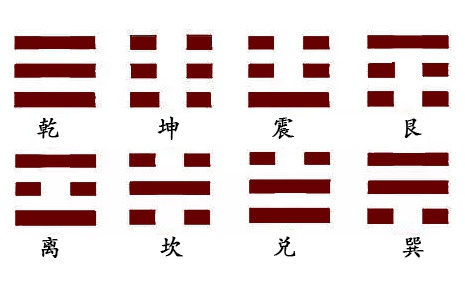
\includegraphics[height=9t,width=9pt, viewport=120 59 225 140,clip]{Eight_Gua.jpeg})为水,
``离''(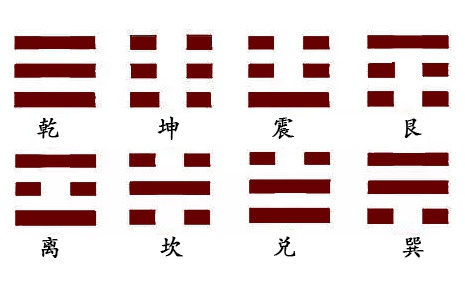
\includegraphics[height=9pt,width=9pt, viewport=5 59 100 140,clip]{Eight_Gua.jpeg})为火。此处寓为``水火既济''之意。}%\protect\hyperlink{fn635}{\textsuperscript{635}}
二字本相调。不觉来到东海道,海水接天浪滔滔。}

{【{\akai 西皮散板}】宝剑扔在东海道,你看我醉仙家的道法高不高?}

{【{\akai 西皮散板}】柳仙带路东海道,万丈波涛走一遭。}

{【{\akai 西皮散板}】湘子说话不中听,丢了宝贝你问旁人。}

{【{\akai 西皮散板}】洞宾主意拿得稳,从今后不管闲事情。}

(李铁拐\hspace{20pt}【{\akai 西皮散板}】$\cdots${}$\cdots${}{入东海道,)}

{【{\akai 西皮散板}】从今后戒酒最为高。}
}

\newpage
\subsubsection{\hei\large 霸王别姬·山头~{\small 之}~ 韩信$^{\ast}$}
\addcontentsline{toc}{subsection}{\hei 霸王别姬~{\small 之}~韩信}

\hangafter=1                   %2. 设置从第1⾏之后开始悬挂缩进  %
\setlength{\parindent}{0pt}{

\setlength{\hangindent}{65pt}{   %3. 设置悬挂缩进量                %
\textrm{【{\akai 西皮散板}】李左车引霸王入了阵道,众诸侯齐奋勇争立功劳。直杀得血成河尸如山倒,灭西楚擒霸王就在今朝。}
}

\setlength{\hangindent}{65pt}{   %3. 设置悬挂缩进量                %
\textrm{【{\akai 西皮散板}】传一令犹如那泰山压倒,兵将涌如那海水临潮。楚项羽犹如那无翼之鸟,失彭城犹如那猛虎离巢。}
}

\setlength{\hangindent}{65pt}{   %3. 设置悬挂缩进量                %
\textrm{【{\akai 西皮散板}】直杀得楚项羽人喊马叫,直杀得子弟兵四路奔逃。直杀得天昏暗日无光耀,直杀得夜更深月挂松梢。}
}

\textrm{(项羽\hspace{25pt}~ 【{\akai 西皮散板}】越杀越勇心焦躁,)}

\textrm{【{\akai 西皮散板}】三军带马回营道,请出张良作计较。}
}

\newpage
\phantomsection %实现目录的正确跳转
\section*{\hei\large 逍遥津~{\small 之}~汉献帝$^{\ast}$}
\addcontentsline{toc}{section}{\hei 逍遥津~{\small 之}~汉献帝}

\hangafter=1                   %2. 设置从第1⾏之后开始悬挂缩进  %
\setlength{\parindent}{0pt}{

【{\akai 二黄导板}】苦汉帝在后宫伤心难忍,

【{\akai 回龙}】父子们悲切切好不伤情,贤御妻呀。

\setlength{\hangindent}{52pt}{   %3. 设置悬挂缩进量                %
【{\akai 二黄原板}】叹伏后此时间必定丧命,我君妃生离散惨不忍闻。二皇儿年幼小孩童天性,哭啼啼与孤王要他的娘亲。想奸贼不由孤咬牙愤恨,上欺寡人下压群臣。欺寡人贼带剑上殿孤见他不敢责问,欺寡人贼独霸朝纲、目无君王、自专自尊。欺寡人孤只得百般谨慎,欺寡人孤只得时刻留心。欺寡人贼奏本是非曲直孤不敢争论,欺寡人孤有命贼大胆妄为抗旨不遵。欺寡人贼一意孤行孤不敢过问,欺寡人孤怒不敢言、忍耐在心。欺寡人孤见他气色不正吓得孤乱了方寸,欺寡人孤见他带怒发威吓得孤胆战心惊。欺寡人蹂躏百般、万分难忍,欺寡人贼败坏朝纲、逆了五伦。欺寡人好一似【{\footnotesize 转}{\akai 二黄慢板}】奴仆受训,欺寡人好一似虐待家人。欺寡人好一似无辜良民被贼围困,欺寡人好一似冤屈罪犯无处冤申。欺寡人好一似蛇毒蝎狠,欺寡人好一似虎咽狼吞。欺寡人好一似前世冤孽今生报应,欺寡人好一似狭路相逢对头仇人。欺寡人好一似阎君索命,欺寡人好一似饿鬼孤魂。欺寡人好一似败阵残兵无投奔,反被贼困垓心难逃遁难存身,坐以待毙谁来救应,
}

【{\akai 二黄散板}】又听得一片喧哗声震乾坤。}

\vspace{15pt}
{\hei 附注}:~

\setlength{\parindent}{0pt}{
《顺天时报》曾刊《逍遥津任辰辙之唱词》一文,所载词句与刘曾复先生所传词句非常相近,照录供参考(张斯琦{\scriptsize 君}提供)
}

\vspace{10pt}
{\centerline{\textcolor{blue}{\hei《逍遥津》``任辰''辙之唱词}}}
\vspace{10pt}

\setlength{\parindent}{22pt}{     %
	{\hwfs 旧本《逍遥津》,``欺寡人''一段,俱用``由求''辙,戏中汉献帝唱``欺寡人好一比鹰抓兔胁''句,过于俚俗,殊伤大雅。刘鸿升未故时,将``由求''改``任辰'',虽亦不免俗,但较旧本,似觉雅驯。李桂芬唱《逍遥津》,亦用斯词,爰将改词录于左端:~}}

\vspace{15pt}
\setlength{\parindent}{0pt}{
	{\hei 汉献帝在后宫伤心难忍,可叹我父子们悲切切冷清清、求生不得求死不能、好不惨情。叹伏后到此时难保活命,我君妃生离散惨不忍闻。二皇儿年幼小孩童之性,哭啼啼与孤王要他的娘亲。想奸贼不由孤嚼牙愤恨,上欺天子下压群臣。欺寡人(贼)带剑上殿孤见他不敢责问,欺寡人(贼)独霸朝纲、目无君、自耑自尊。欺寡人孤只得百般谨慎,欺寡人孤只得时刻留神。欺寡人(贼)奏本是非曲直孤不敢\textcolor{red}{$\square~\square$},欺寡人孤有命贼大胆妄为抗旨不遵。欺寡人贼自由行孤不敢过问,欺寡人孤怒不敢言、忍耐在心。欺寡人孤见他气色不正嚇得孤乱了方寸,欺寡人孤见他怒发威嚇得吊胆提心。欺寡人蹂躏百般、惨忍万分,欺寡人贼败坏纲常、逆了五伦。欺寡人好一似主仆受训,欺寡人好一似虐待家人。欺寡人好一似无辜良民被贼围困,欺寡人好一似冤屈罪犯\textcolor{red}{$\square$}而受刑。欺寡人好一似蛇毒蝎狠,欺寡人好一似虎狼把孤吞。欺寡人好一似前世冤孽今生报应,欺寡人好一似夹路相逢对头仇人。欺寡人好一似阎王索命,欺寡人好一似饿鬼勾魂。欺寡人好一似败阵惨兵无投奔,反被贼困垓心、难逃命、难生存、认贼斩、恁贼擒,孤做一待毙谁来救应,又听得宫门外喧哗之声。
}}


\addcontentsline{toc}{section}{\hfill[\hei 附录]\hfill}
\newpage
\chead{附~录} % 页眉中间位置内容
\textbf{柴桑口}\protect\hyperlink{fn636}{\textsuperscript{636}}

{[}第一场{]}

(四文堂,刘备、诸葛亮上)

刘备 {[}引子{]}祸福惟天造,岂在人谋计巧。

诸葛亮
{[}引子{]}秦、崔玉童\protect\hyperlink{fn637}{\textsuperscript{637}}到,从此知音稀少。

诸葛亮 参见主公。

刘备 先生少礼,请坐。

诸葛亮 谢座。

刘备
(念)周战场中祸难平,岂知转福结□□。\protect\hyperlink{fn638}{\textsuperscript{638}}

诸葛亮 (念)自古辛勤有天下,不在人谋定相星。

刘备 孤,刘备。

诸葛亮 山人诸葛亮。

刘备 先生。

诸葛亮 主公。

刘备
日前周郎设下``假途灭虢''之计,被先生奇谋,只气得他喷血坠马\protect\hyperlink{fn639}{\textsuperscript{639}},此时未闻周郎吉凶如何。

诸葛亮 亮夜观天象,见将星坠落。我料周郎刻下必死无疑也。

刘备 此话难料。

旗牌 (内)走哇。

(旗牌上)

旗牌
启上主公,昨日命小人持书递进吴营,周瑜拆开一观,忽然呕吐气绝身亡。今将灵柩移至柴桑去了。

诸葛亮 如何。

刘备 知道了。

诸葛亮 退下。

(旗牌下)

刘备 果然不出先生所料,周郎已死,还当如何?

诸葛亮
我料代周郎之权必是鲁肃。亮观天象,见将星聚在东吴,我当以过江吊孝为由,好觅贤士辅佐\protect\hyperlink{fn640}{\textsuperscript{640}}主公。

刘备
且慢,东吴将士恨先生如入骨髓,此番前去,必遭其害。且莫做那披麻救火,自惹其祸。

诸葛亮
周瑜在日,亮犹不惧,今瑜(已)死\protect\hyperlink{fn641}{\textsuperscript{641}},何足惧哉?

刘备 去得的?

诸葛亮 去得的。

刘备 无妨事?

诸葛亮 无妨事。

刘备
孤放心不下,可命三弟带领铁骑一万,战船千只,跟随先生前往。孤也好放心。

诸葛亮
既蒙主公垂念,就命四将军子龙随我前往,可命三将军在江南岸上等候。山人吊祭已毕,过江之时,用羽扇一招,前来接应便了。

刘备 先生呐。

刘备
【西皮散板\protect\hyperlink{fn642}{\textsuperscript{642}}】非是孤王人安顿,东吴尽是豺狼虎群。此番前去稍有伤损,岂不教孤两离分\protect\hyperlink{fn643}{\textsuperscript{643}}。

诸葛亮
【西皮散板\protect\hyperlink{fn644}{\textsuperscript{644}}】时不到兴与衰天心造定,当治乱自有那一辈时人。【转西皮快板】天生来周公瑾吴邦英俊,偏又有诸葛亮汉室称臣。三江口协力时同把曹併,彼爱我我爱彼各无异心。他起意三次里害我性命,心未遂气得他丧了残生。在帐中施一礼主心安稳,

刘备 先生保重了。

诸葛亮 【西皮散板】但看我一叶飘如风送云。

刘备
【西皮散板】他那里坦然不虑心安稳,孤心中不定胆战心惊。但愿得此一去吉星照定,且待他无凶险也好放心。

(同下)

{[}第二场{]}

(四白文堂、二旗牌、鲁肃上)

鲁肃
【西皮摇板\protect\hyperlink{fn645}{\textsuperscript{645}}】伤我那擎天柱一旦早丧,眼见得我东吴谁是栋梁。蒙主恩虽与我兵权执掌,愧匪才怎做得治国安邦。

鲁肃
下官鲁肃,不料孔明用计,竟将公瑾气死。蒙公瑾生前已奏表章,举我统领兵权。唉,我自愧匪才,焉能掌此大权,无奈主公再三\protect\hyperlink{fn646}{\textsuperscript{646}},难以推却,只得勉力而为。今将公瑾灵柩移至柴桑,等候他子周循\protect\hyperlink{fn647}{\textsuperscript{647}}到来,成服\protect\hyperlink{fn648}{\textsuperscript{648}}丧葬也。

四将 (内)走哇。

(四将上)

四将 参见都督。

鲁肃 列公少礼。

(鲁肃看介)

鲁肃 列公怒气不息,进帐何事?

四将
启禀都督,今有孔明带了祭礼前来祭奠先帅,故而进帐请教都督:还是将孔明杀了后祭,还是祭了后杀呢?

鲁肃 哦,那孔明竟敢前来吊祭先帅么?

四将 正是。

鲁肃 他带了多少人马?

四将 只有一叶扁舟,并无人马。

鲁肃 只有一叶扁舟,并无人马?

四将 正是。

鲁肃
(冷笑介)哼,呵呵\ldots{}\ldots{}这厮又来作怪。我东吴将士恨不得食尔之肉,他偏偏驾一叶扁舟而来。孔明啊孔明,你今前来岂不是羊入虎口。不知列公心意如何?

四将
吾家先帅被他气死,恨不得手刃此贼\protect\hyperlink{fn649}{\textsuperscript{649}}。他今自寻前来,都督传令可将他剖腹挖心\protect\hyperlink{fn650}{\textsuperscript{650}},活祭先帅,以报此仇。

鲁肃
不可。他今前来,定有一番道理。若凶惧而杀之,天下人道我东吴无容人之量。且待他祭奠之后,先用言语责他,然后治死也还不迟。不知列公意下如何?

四将 只是教那贼多活一时。

赵云 (内)孔明先生到。

鲁肃 列公不可造次,当遵吾令。

四将 遵命。

鲁肃 有请。

四将 有请。

(赵云、童儿、诸葛亮上)

鲁肃 先生。

诸葛亮 都督。

鲁肃 呀,先生一别有年,使人梦想。

诸葛亮
{久未晤面}(或:久违教益),如有所亡\protect\hyperlink{fn651}{\textsuperscript{651}}。

鲁肃
荷蒙\protect\hyperlink{fn652}{\textsuperscript{652}}足下远来吊祭,足见多情。

诸葛亮 故交之谊,聊此一行,以表寸意。

鲁肃 多谢了。

诸葛亮 先灵供在何处?

鲁肃 现在后帐。待下官引路。

诸葛亮 有劳了。

(同下)

{[}第三场{]}

(又上)

诸葛亮
\textless{}\textbf{三叫头}\textgreater{}公瑾,先生,唉,都督哇,呃\ldots{}\ldots{}(哭介)

诸葛亮
【二黄导板\protect\hyperlink{fn653}{\textsuperscript{653}}】{见陵寝}(或:见灵寝)不由人泪如雨降,想俊容不由人痛断肝肠。

诸葛亮
\textless{}\textbf{三叫头}\textgreater{}公瑾,先生,唉,都督哇,呃\ldots{}\ldots{}(哭介)

诸葛亮 【二黄散板】可惜你钟山秀{春年正旺}(或:春华正旺),

诸葛亮
【反二黄原板\protect\hyperlink{fn654}{\textsuperscript{654}}】可惜你美英才一旦夭亡。可惜你空碌碌一生容让,可惜你兢业业半世奔忙。实指望併曹瞒你我安享,\textless{}\textbf{哭头}\textgreater{}都督哇\ldots{}\ldots{}

诸葛亮
【反二黄原板】又谁知黄粱梦\protect\hyperlink{fn655}{\textsuperscript{655}}昙花一场。

旗牌 进位,上香,鞠躬。跪,叩首,二叩首,三叩首。兴,鞠躬。

赵云 (念)
呜呼公瑾,不幸夭亡!寿短固天,人岂不伤!我心实痛,酬酒一觞;君其有灵,想我衷肠。

诸葛亮
公瑾,想你英雄盖世,一代风流。贯精忠于日月,秉赤胆与东吴。不幸一旦身故,未遂你胸中之志,好不遗恨人也。

诸葛亮
【反二黄慢板\protect\hyperlink{fn656}{\textsuperscript{656}}】你是个霸业的忠贞良将,你是个振东吴豪杰贤良。谁似你天生来高智雅量,谁似你文武略器宇轩昂。谁似你青年人兵权执掌,谁似你定霸业扶弱抑强。奸曹贼统雄兵如风似浪\protect\hyperlink{fn657}{\textsuperscript{657}},只吓得江南士束手要降。若非你怀大志陈兵相抗\protect\hyperlink{fn658}{\textsuperscript{658}},运机谋烧得他抛甲弃枪。到今日稍得遂太平景象\protect\hyperlink{fn659}{\textsuperscript{659}},转瞬间\protect\hyperlink{fn660}{\textsuperscript{660}}天不佑大厦断梁。抛得我故人儿将谁依傍,\textless{}\textbf{哭头}\textgreater{}公瑾呐\ldots{}\ldots{}

诸葛亮
【反二黄原板】闪得我前后事与谁商量。今日里原比作那伯仲情况,我与你又好比鸡黍范、张\protect\hyperlink{fn661}{\textsuperscript{661}}。{望阴灵鉴吾这虔诚祭享,虔诚祭享,泪纷纷捧玉樽享受烝尝。}(或:望阴灵鉴之我祭奠,知我祭奠,诸葛亮泪纷纷痛断肝肠。\protect\hyperlink{fn662}{\textsuperscript{662}})

旗牌 进位,上香,退,鞠躬。

赵云
(念)呜呼公瑾!生死永别!朴守其真,冥冥灭灭,君如有灵,乞见我心:从此天下,更无知音!呜呼痛哉,伏惟上享。

诸葛亮 公瑾呐\ldots{}\ldots{}

诸葛亮
【反二黄散板】你非是妒贤辈胸怀愚量,都只是各为主不得不防。到今日奸曹在你命身丧,\textless{}\textbf{哭头}\textgreater{}都督哇\ldots{}\ldots{}

诸葛亮
【反二黄散板】闷得我诸葛亮心意彷徨。思至此哭得我{咽喉气颡}(或:咽喉难让),

众
【反二黄散板】只哭得满营中泪洒千行。\protect\hyperlink{fn663}{\textsuperscript{663}}

鲁肃 先生且免悲伤,还当同心破曹要紧。

众 是呀,同心破曹,全仗先生。

诸葛亮
亮纵有千言万语,一时难以尽诉。列公以奸曹为念,亮当佩服,与公同心破曹,就此告辞了。

鲁肃 且慢,备得水酒,聊表地主之情。

诸葛亮 本当领受,怎奈有公务在身,告辞了。

鲁肃 有慢了。

诸葛亮 \textless{}\textbf{叫头}\textgreater{}公瑾!

诸葛亮 你若有灵,须见我心呐!

诸葛亮 【反二黄散板】心问口、口问心牢骚千状,有万篇写不尽我心哀伤。

(诸葛亮出门)

众 送先生。

诸葛亮 【反二黄散板】送千里终须别何须谦让,

鲁肃 恕不远送了。

(赵云下)

诸葛亮
【反二黄散板】试看我一帆风雨洒康庄\protect\hyperlink{fn664}{\textsuperscript{664}}。

(诸葛亮下)

鲁肃 【反二黄散板】他那里诚恳恳哀泣模样,为朋友可算得古道热肠。

鲁肃 列公,人言先帅与孔明不睦,今日一见真乃伤情。

众 看将起来,诸葛先生乃是大大的好人。

二旗牌 (内)走哇。

(二旗牌上)

二旗牌 公子到。

鲁肃 有请。

众 有请。

(周循上)

周循 伯父。

鲁肃 公子,不知公子驾到,未曾远迎,面前恕罪。

周循 岂敢。小侄来的鲁莽,伯父、众位伯父恕罪。

众 岂敢。

周循 我父灵堂今在何处?

鲁肃 现在后帐,随我来。

周循 有劳伯父。

(同一翻两翻,周循看介、哭介)

周循 唉,爹爹呀\ldots{}\ldots{}(哭介)

周循 【二黄散板】在灵位不由我死去又醒,

周循
\textless{}\textbf{三叫头}\textgreater{}爹爹,我父,唉,爹爹呀\ldots{}\ldots{}(哭介)

周循
【二黄散板】想今生要见面万万不能。为国家受尽了千般苦衷,谁信那青史上万载标名。

鲁肃 啊公子,先帅已死,不能复生,请自保重要紧。

众 是啊,请自保重要紧。

周循 诚领众位伯父之教,小侄敢不从命。啊伯父,小侄有一言不知可听否?

鲁肃 公子有话请讲。

周循
先父执掌兵权有年,不料被孔明三气而死,我与他不共戴天之仇,望伯父助小侄一膀之力,杀往荆(州\protect\hyperlink{fn665}{\textsuperscript{665}}),生擒孔明,与我父报仇雪恨。伯父料无推辞的了。

鲁肃 啊公子,那孔明乃是个好人。

周循 啊?怎见得他是好人?

鲁肃 他闻先帅已死,过得江来哭了又祭,祭了又哭,岂不是个好人?

周循 啊,那孔明几时来的?

鲁肃 方才在此。

周循 如今何在?

鲁肃 回往荆州去了。

周循 啊伯父,你要与我统领人马追杀孔明,如若不然,我就碰死在灵前。

众 公子不必如此,大家追杀孔明便了。

周循 好,快快追赶。

鲁肃 去不得。

(同下)

{[}第四场{]}

(赵云、童儿、诸葛亮上)

诸葛亮
【西皮散板】非是我笑他们无有志量,怎知我袖儿内暗有行藏。{遇不着智谋人心中惆怅}(或:将身儿来至在江边岸上),

(庞统上)

庞统 呔,你往哪里走。

庞统 【西皮散板】你纵有托天手(或:托天胆)难逃罗网。

庞统
孔明呐孔明,你用计将周郎三气而死,又假意过江吊祭,分明笑我东吴无有能人。来来来,我与你较量。

诸葛亮 原来是凤雏先生。先生平生大才,今日出此不经之言,故意吓我。

诸葛亮、庞统 哈哈,哈哈,啊哈哈哈\ldots{}\ldots{}(诸葛亮、庞统对笑介)

诸葛亮
啊先生,我此来实为吾兄,我料仲谋必不能重用足下,玄德公宽仁厚德,(不负\protect\hyperlink{fn666}{\textsuperscript{666}})公生平所学,我有草书一封,趁便即往\protect\hyperlink{fn667}{\textsuperscript{667}}荆州共扶汉室,名垂千古,岂不美哉?

庞统
承蒙美意,自得遵教\protect\hyperlink{fn668}{\textsuperscript{668}}。

(起\textless{}\textbf{鼓架子}\textgreater{},诸葛亮、庞统两望)

庞统 啊先生,看那旁人声呐喊,必是周循追赶前来。

诸葛亮 公且自回避,亮要登舟去了。

庞统 后会有期。

诸葛亮 请呐。

诸葛亮 【西皮散板】此时节说不尽话言惆怅,

庞统 【西皮散板】暂分别改日里再会荆襄。

(庞统下)

诸葛亮 哈哈哈\ldots{}\ldots{}(笑介)

诸葛亮
【西皮散板】想人生荣与枯得失难量,际风云{显奇谋}(或:显奇能)姓字名扬。望一派{白茫茫}(或:白亮亮){翻江波浪}(或:滔天波浪),

张飞 (下场门内)嘚,开船。

(四黑龙套、二船夫、张飞上)

张飞 【西皮散板】张翼德接先生来到长江。

张飞 先生,搭了扶手。

(诸葛亮、赵云、童儿上船介;四白文堂、四将、周循上)

周循 呔,船头之上,可是诸葛亮?

诸葛亮 然也,来者何人?

周循 俺乃公瑾之子周循是也。

诸葛亮 哦,原来是公子到了,敢莫是与父谢孝的么?

周循 正是。

诸葛亮 为何持戈相向,是何理也?

周循 请先生上岸,周循有话言讲。

诸葛亮
哼呵呵呵\ldots{}\ldots{}(冷笑介)我若上岸,只恐你那小性命必随儿父去也。

周循 呔,孔明你若不上岸,休怪周循无礼了。

张飞
呔,我把你这不孝的乳臭小儿,汝父既死,儿不居守灵帐,执持器械,何以成孝?你这不忠不孝、不仁不义之人,要儿何用!先生闪开,待咱老张将他射死也。

诸葛亮 不可,饶他这条小命去罢。

张飞 也罢,念尔有重孝在身,暂且饶儿不死。嘚,开船!

(张飞三笑,诸葛亮众下)

周循 苍天呐苍天,

周循
【西皮摇板\protect\hyperlink{fn669}{\textsuperscript{669}}】满江洒下青丝网,怎奈鱼儿又脱缰。

周循 罢!

(周循跳水介,四将拦介)

四将 公子不必如此,驾船追杀孔明便了。

周循 好。驾船追者!

(同下)

注:钞本中诸葛亮祭奠周瑜的祭文,个别词句与《三国演义》原文音同字异,今将《三国演义》中诸葛亮祭文附后:

\textbf{呜呼公瑾,不幸夭亡!修短故天,人岂不伤?}

\textbf{我心实痛,酹酒一觞;君其有灵,享我烝尝!}

\textbf{吊君幼学,以交伯符;仗义疏财,让舍以民。}

\textbf{吊君弱冠,万里鹏抟;定建霸业,割据江南。}

\textbf{吊君壮力,远镇巴丘;景升怀虑,讨逆无忧。}

\textbf{吊君丰度,佳配小乔;汉臣之婿,不愧当朝,}

\textbf{吊君气概,谏阻纳质;始不垂翅,终能奋翼。}

\textbf{吊君鄱阳,蒋干来说;挥洒自如,雅量高志。}

\textbf{吊君弘才,文武筹略;火攻破敌,挽强为弱。}

\textbf{想君当年,雄姿英发;哭君早逝,俯地流血。忠义之心,英灵之气;命终三纪,名垂百世,哀君情切,愁肠千结;惟我肝胆,悲无断绝。}

\textbf{昊天昏暗,三军怆然;主为哀泣;友为泪涟。亮也不才,丐计求谋;助吴拒曹,辅汉安刘;}

\textbf{掎角之援,首尾相俦,若存若亡,何虑何忧?}

\textbf{呜呼公瑾!生死永别!朴守其贞,冥冥灭灭,魂如有灵,以鉴我心:从此天下,更无知音!}

\textbf{呜呼痛哉!伏惟尚飨。}

\newpage
\subsubsection{铁笼山·迷当发点~\protect\footnote{根据刘曾复先生钞录本整理。钞本作``铁龙山'',此处从《三国演义》原文。}}%\protect\hyperlink{fn670}{\textsuperscript{670}}
\addcontentsline{toc}{subsection}{\hei 铁笼山·迷当发点}

\hangafter=1                   %2. 设置从第1⾏之后开始悬挂缩进  %
\setlength{\parindent}{0pt}{
%{\centerline{\textrm{{[}\hei 第一场{]}}}}

	(\textless{}\!{\bfseries\akai 水龙吟}\!\textgreater{}{\hwfs 四}蛮兵、{\hwfs 二丑}校尉{\hwfs 站门};~\textless{}\!{\bfseries\akai 四击头}\!\textgreater{}迷当{\hwfs 上})

迷当\hspace{30pt} \textless{}\!{\bfseries\akai 点绛唇}\!\textgreater{}西羌英豪,儿郎虎豹,统雄骁,族裔三苗,灭魏蜀汉保。

(\textless{}\!{\bfseries\akai 水龙吟}{\akai 合头}\!\textgreater{}迷当{\hwfs 上高台},{\hwfs 坐})

迷当\hspace{30pt} ({\akai 念})三国纷纷起战争,孔明火烧藤甲兵。七擒孟获孤得见,西羌领兵到如今。

\setlength{\hangindent}{60pt}{   %3. 设置悬挂缩进量                %
迷当\hspace{30pt} 孤,西羌国王迷当,长子迷强、次子迷能俱丧陈泰之手,为此每日操练人马,以防不测。看今日天气晴和,不免去往草上坡行围射猎,孩子们、马夫们走上。
}

(内\hspace{35pt} 马夫们走上。)

({\hwfs 四}马夫{\hwfs 上})

\setlength{\hangindent}{60pt}{   %3. 设置悬挂缩进量                %
四马夫\hspace{20pt} ({\akai 念})\textless{}\!{\bfseries\akai 马夫赞}\!\!\textgreater{}生来本是西凉娃,穿山越岭骑劣马。冲锋陷阵咱不怕,途程当玩耍,途程当玩耍。({\hwfs 边走边念})
}

四马夫\hspace{20pt} 参见大王。

迷当\hspace{30pt} 传蛮女们进见。

(马夫{\hwfs 下},马夫甲、乙、丙、丁{\hwfs 先后各拉}蛮女甲、乙、丙、丁{\hwfs 先后上},{\hwfs 分段唱}\textless{}\!{\bfseries\akai 粉蝶儿}\!\textgreater{})

蛮女甲\hspace{20pt} \textless{}\!{\bfseries\akai 粉蝶儿}\!\textgreater{}异国异苗,

蛮女乙\hspace{20pt} \textless{}\!{\bfseries\akai 粉蝶儿}\!\textgreater{}小蛮婆,异国异苗;

蛮女丙\hspace{20pt} \textless{}\!{\bfseries\akai 粉蝶儿}\!\textgreater{}天生就玉容花貌,

蛮女甲\hspace{20pt} \textless{}\!{\bfseries\akai 粉蝶儿}\!\textgreater{}镇日里舞剑操刀,背弯弓、发硬驽、穿杨技巧。

四蛮女\hspace{20pt} ({\akai 合})\textless{}\!{\bfseries\akai 粉蝶儿}\!\textgreater{}兴来时马上嬉游,弹一曲昭君宫调。

四蛮女\hspace{20pt} 参见大王。

迷当\hspace{30pt} 罢了。

(马夫、蛮女{\hwfs 分站两边})

迷当\hspace{30pt} 孩子们!

(众{\hwfs 应})

迷当\hspace{30pt} 草上坡去者!

(众{\hwfs 应},众{\hwfs 唱分段}\textless{}\!{\akai 北}{\bfseries\akai 泣颜回}\!\textgreater{})

众\hspace{40pt} \textless{}\!{\akai 北}{\bfseries\akai 泣颜回}\!\textgreater{}驱队出西郊,

(众{\hwfs 合龙},迷{\hwfs 下高台},{\hwfs 上马})

众\hspace{40pt} \textless{}\!{\akai 北}{\bfseries\akai 泣颜回}\!\textgreater{}逐骅骝人拥哎咆哮,

(众{\hwfs 转场},迷{\hwfs 上大边高台})

众\hspace{40pt} \textless{}\!{\akai 北}{\bfseries\akai 泣颜回}\!\textgreater{}貔貅簇拥,人如虎生翼英豪。

(众{\hwfs 转场},迷{\hwfs 下高台},{\hwfs 上小边高台})

众\hspace{40pt} \textless{}\!{\akai 北}{\bfseries\akai 泣颜回}\!\textgreater{}旗旛耀日,韵悠悠,画角连珠炮朴咚咚。

(迷{\hwfs 下高台})

众\hspace{40pt} \textless{}\!{\akai 北}{\bfseries\akai 泣颜回}\!\textgreater{}紧擂鼍鼓,布围场满塞弓刀,布围场满塞弓刀。

({\hwfs 归正场})
}

\newpage
\phantomsection %实现目录的正确跳转
\section*{\textrm{美良川 {\small 之} 秦琼}~\protect\footnote{根据刘曾复先生钞录的秦琼``单词本''整理。\\
	\vspace{7pt}
\hangafter=1                   %2. 设置从第1⾏之后开始悬挂缩进  %
\setlength{\parindent}{0pt}{
	此戏花脸唱一支《八声甘州》,据《梅兰芳回忆录:舞台生活四十年》\upcite{Mei-Remember}%\textsuperscript{{[}28{]}.}
记载,词句为:~\\
	\vspace{5pt}
{\hei ``扬威奋勇,看愁云惨惨,杀气腾腾。鞭鞘指处,鬼神尽觉惊恐。三关怒冲千里振,八寨雄兵已成空。旌旗摇,剑戟丛,将军八面展威凤。人似虎,马如龙,伫看一战使成功!''}\\
	\vspace{7pt}
《铁笼山》一剧中姜维唱的《八声甘州》即出自此戏。}
}}%\protect\hyperlink{fn671}{\textsuperscript{671}}
\addcontentsline{toc}{section}{\hei 美良川~{\small 之}~秦琼}

\hangafter=1                   %2. 设置从第1⾏之后开始悬挂缩进  %
\setlength{\parindent}{0pt}{
{\centerline{\textrm{{[}\hei 第一场{]}}}}
\vspace{5pt}

({\hwfs 上})

({\akai 念})头戴金盔凤翅飘,身穿铠甲络丝绦。劈抡双锏无人抵,保定我主锦龙朝。

俺,姓秦名琼字叔宝,唐室驾前为臣。奉主之命跟随二主千岁大战刘武周,可恨那贼战又不战,降又不降。今日闲暇无事,不免到二主营中问安。

吓!进得营来为何这样静悄悄的,待我两厢问来。三军们,主公可在营中?

哪里去了?

何人保驾?

不好了!

且住!二主夜探白璧关\footnote{刘曾复先生钞本作``北璧关'',此处从《说唐全传》;历史上李世民破刘武周麾下尉迟敬德于美良川,是其平定北方割据势力刘武周、宋金刚的关键战役(柏壁之战)的一部分,《旧唐书》、《新唐书》和《资治通鉴》均有记载。}%\protect\hyperlink{fn672}{\textsuperscript{672}}
,咬金保驾岂是那黑贼对手?众将官,迎上前去。({\hwfs 下})

\vspace{3pt}{\centerline{\textrm{{[}{\hei 第二场}{]}}}}\vspace{5pt}

({\hwfs 上})

呔!尔有何本领,擅敢追杀我主?

若问你老爷的,尔且听道。

呔!尔敢是怯战?你我两厢问来。

三军的,哪里宽阔?

打道美良川。({\hwfs 下})

\vspace{3pt}{\centerline{\textrm{{[}{\hei 第三场}{]}}}}\vspace{5pt}

({\hwfs 上})

来到美良川,你我怎样比试?

下得马来,何以为赌?何为打鞭换锏?

如此说来老爷先打。

老爷先打。

好,你我两厢问来。

三军的,何处地界?

黑贼,乃是我唐室地界,还是老爷先打。

哼!老爷打了就无有尔的份了。让尔先打。

这作什么?

你老爷站得稳,尔只管的打。

吐什么?

你老爷焉有吐红之理?尔只管的打。

又吐什么?

你老爷方才言过焉有吐红之理,尔只管的打。

你敢有逃走之意?若要你老爷不打,除非在老爷胯下趱将过去,俺便饶尔不死。

当真要打?

果然要打?

要打?

起鼓招打。

呔!尔为何闪你老爷这头一锏?

九十斤一根,

慢说是两锏,就是这一锏也要结果尔的性命。

当真要打?

果然要打?

要打?

起鼓招打\footnote{刘曾复先生钞本作``起鼓照打'',此处从段公平{\scriptsize 君}建议,为上下文统一改。}
%\protect\hyperlink{fn673}{\textsuperscript{673}}
。

与你老爷吐,吐红。

起鼓招打。

带马。({\hwfs 追下})

\vspace{3pt}{\centerline{\textrm{{[}{\hei 第四场}{]}}}}\vspace{5pt}

({\hwfs 上})

前道为何不行?

人马列开。

【{\akai \textcolor{red}{西皮摇板}\footnote{刘曾复先生钞本未注明板式。}%\protect\hyperlink{fn674}{\textsuperscript{674}
}】秦琼生来不可当\footnote{``不可当''犹言``不得了''之意。}
%\protect\hyperlink{fn675}{\textsuperscript{675}}
,美良川前摆战场。三鞭打不动秦叔宝,两锏打得他吐红光。

败兵不可追赶,人马回营。({\hwfs 下})}


\newpage
\phantomsection %实现目录的正确跳转
%\hypertarget{ux53d6ux91d1ux9675-ux4e4b-ux66f9ux826fux81e3}{%
\section*{\large\hei 取金陵~{\small 之}~曹良臣}%\label{ux53d6ux91d1ux9675-ux4e4b-ux66f9ux826fux81e3}}
\addcontentsline{toc}{section}{\hei 取金陵~{\small 之}~曹良臣}

\hangafter=1                   %2. 设置从第1⾏之后开始悬挂缩进  %
\setlength{\parindent}{0pt}{
{\centerline{\textrm{{[}\hei 第一场{]}}}}
\vspace{5pt}

({\akai 念})威震金陵谁敢犯,一片丹心保皇朝。

本帅,曹良臣。

今有红巾贼寇,兴兵犯境。自古道:兵行千里,不战自倦。今晚末将带兵前去劫营。都督大兵随后接应,大功必成也。

得令!

【{\akai 西皮摇板}\footnote{刘曾复先生钞本未注明板式,下同。}%\protect\hyperlink{fn676}{\textsuperscript{676}}
】都督传令如雷吼,扫灭红巾统貔貅。三军带马出帐口,不灭红巾誓不休。

\vspace{3pt}{\centerline{\textrm{{[}{\hei 第二场}{]}}}}\vspace{5pt}

【{\akai 西皮摇板}】旌旗招展绕星斗,金枪一举鬼神愁。三军催马朝前走,抬头只见一营头。

踹营!

哎呀!

【{\akai 西皮摇板}】只望劫营能成就,谁知贼有巧机谋。三军随爷绕营走,

\vspace{3pt}{\centerline{\textrm{{[}{\hei 第三场}{]}}}}\vspace{5pt}

【{\akai 西皮摇板}】适才闪出红巾寇,不由怒火起心头,三军催马踹营走,

杀!

哎呀!

【{\akai 西皮摇板}】只望今晚擒贼首,又恐中贼奸机谋。三军随爷夺路走,

\vspace{3pt}{\centerline{\textrm{{[}{\hei 第四场}{]}}}}\vspace{5pt}

【{\akai 西皮摇板}】四面俱是红巾寇,口口叫我把降投。东杀、西挡无路走------

然!

答话者何人?

唔哙呀!闻得徐达用兵如神,果然话不虚传。此乃天教俺归降也!

【{\akai 西皮摇板}】人言徐达韬略有,提兵调将似武侯。甩镫离鞍卸甲胄,含羞带愧把他投。

归降来迟,死罪呀死罪。

赤福寿人马,元帅要提防一二。\footnote{刘曾复先生钞本注明``以上《取金陵》曹良臣''。刘曾复先生钞本未注明场次,有关场次安排据《京剧汇编》第十九集~阎庆林~藏本,该藏本系阎岚秋(九阵风)生前演出本。}%\protect\hyperlink{fn677}{\textsuperscript{677}}
}

\item
  \leavevmode\hypertarget{fn636}{}%
  根据刘曾复先生钞录本整理。刘曾复先生钞本注``马少山本,民廿九 1940
  王存''。段公平君按:据何毅老师介绍,刘曾复先生本有意为此剧本润色文辞,后因言派《卧龙吊孝》已流行,``我就别招这个讨厌了'',竟未完成。因此抄本中讹误脱漏较多,且多有刘曾复先生修改和原文并存痕迹。这次整理,在文辞通顺的基础上拟对这些痕迹适当保留。刘曾老所改录在正文,抄本原文录在脚注中。抄本整理过程中,幸得``小豆子''老师惠赐《柴桑口》余胜荪藏本扫描件,和此抄本同质性很高,故多用为参考。\protect\hyperlink{fnref636}{↩}
\item
  \leavevmode\hypertarget{fn637}{}%
  秦即地狱秦广王,专司人间夭寿;崔即判官崔钰,掌生死簿。刘曾复先生钞本中,``童''字不确认,疑``章''字;玉童,即仙童。\protect\hyperlink{fnref637}{↩}
\item
  \leavevmode\hypertarget{fn638}{}%
  刘曾复先生钞本``周''字不确认,亦欠通;``结''字不确认,后二字缺。段公平君按:据余胜荪藏本,此四句诗为``干戈有时化玉帛,蜀吴修好结姻亲。炎汉正统有天相,不须人谋定隆兴。''和此本中的诗应该颇相关。因此推断第二句所缺两字也是``姻亲''之类。第一句``难''字不能确认,或疑为``虽'',结合文意,作``难''字似乎较合理。\protect\hyperlink{fnref638}{↩}
\item
  \leavevmode\hypertarget{fn639}{}%
  段公平君按:刘曾复先生钞本作``赞马'',似欠通,今据文意及《京剧汇编》第九十三集
  余胜荪藏本改。\protect\hyperlink{fnref639}{↩}
\item
  \leavevmode\hypertarget{fn640}{}%
  刘曾复先生钞本作``扶佐''。\protect\hyperlink{fnref640}{↩}
\item
  \leavevmode\hypertarget{fn641}{}%
  刘曾复先生钞本作``今瑜死``,此处从《三国演义》原文。\protect\hyperlink{fnref641}{↩}
\item
  \leavevmode\hypertarget{fn642}{}%
  刘曾复先生钞本未注明西皮或二黄板式,今据后文及《京剧汇编》第九十三集
  余胜荪藏本推测。\protect\hyperlink{fnref642}{↩}
\item
  \leavevmode\hypertarget{fn643}{}%
  刘曾复先生钞本``教''、``两''二字不确认,据文意推断。\protect\hyperlink{fnref643}{↩}
\item
  \leavevmode\hypertarget{fn644}{}%
  刘曾复先生钞本注``散(板)转快(板)或二六''。\protect\hyperlink{fnref644}{↩}
\item
  \leavevmode\hypertarget{fn645}{}%
  刘曾复先生钞本未注明板式,今据《京剧汇编》第九十三集
  余胜荪藏本添。\protect\hyperlink{fnref645}{↩}
\item
  \leavevmode\hypertarget{fn646}{}%
  刘曾复先生钞本原文如此,文意欠通。\protect\hyperlink{fnref646}{↩}
\item
  \leavevmode\hypertarget{fn647}{}%
  刘曾复先生钞本作``周巡'',此处从《三国演义》原文,作``周循''。\protect\hyperlink{fnref647}{↩}
\item
  \leavevmode\hypertarget{fn648}{}%
  旧时死者入殓后,其亲属穿着符合各自身分的丧服,称为``成服''。\protect\hyperlink{fnref648}{↩}
\item
  \leavevmode\hypertarget{fn649}{}%
  刘曾复先生钞本作``千刃此贼'',此处据《京剧汇编》第九十三集
  余胜荪藏本改。\protect\hyperlink{fnref649}{↩}
\item
  \leavevmode\hypertarget{fn650}{}%
  刘曾复先生钞本作``破腹挖心''。\protect\hyperlink{fnref650}{↩}
\item
  \leavevmode\hypertarget{fn651}{}%
  刘曾复先生钞本原录``如有所望'',后改``如有所忘'',段公平君注:``如有所忘''文意欠通。应为``如有所亡'',即``如有所失''意。\protect\hyperlink{fnref651}{↩}
\item
  \leavevmode\hypertarget{fn652}{}%
  荷蒙,犹``承蒙''之意。\protect\hyperlink{fnref652}{↩}
\item
  \leavevmode\hypertarget{fn653}{}%
  刘曾复先生钞本注``导(板)或散(板)''\protect\hyperlink{fnref653}{↩}
\item
  \leavevmode\hypertarget{fn654}{}%
  刘曾复先生钞本注``以下散(板)或反二黄原板''\protect\hyperlink{fnref654}{↩}
\item
  \leavevmode\hypertarget{fn655}{}%
  刘曾复先生钞本作``大数到'',此处据《京剧汇编》第九十三集
  余胜荪藏本改。\protect\hyperlink{fnref655}{↩}
\item
  \leavevmode\hypertarget{fn656}{}%
  刘曾复先生钞本仅注反二黄,今据《京剧汇编》第九十三集
  余胜荪藏本添。\protect\hyperlink{fnref656}{↩}
\item
  \leavevmode\hypertarget{fn657}{}%
  刘曾复先生钞本原录``暗兵机如风波浪'',先生改为``统雄兵如风似浪''。\protect\hyperlink{fnref657}{↩}
\item
  \leavevmode\hypertarget{fn658}{}%
  刘曾复先生钞本原录``沉兵相挡'',先生改为``陈兵相抗''。\protect\hyperlink{fnref658}{↩}
\item
  \leavevmode\hypertarget{fn659}{}%
  刘曾复先生钞本原录``烧得谁太平青浪'',先生改为``稍得遂太平景象''。\protect\hyperlink{fnref659}{↩}
\item
  \leavevmode\hypertarget{fn660}{}%
  刘曾复先生钞本原录``话未了'',先生改为``转瞬间''。\protect\hyperlink{fnref660}{↩}
\item
  \leavevmode\hypertarget{fn661}{}%
  ``范张鸡黍''指范式、张劭一起喝酒食鸡。比喻朋友之间情义与深情。刘曾复先生钞本记作``稷黍范张''。\protect\hyperlink{fnref661}{↩}
\item
  \leavevmode\hypertarget{fn662}{}%
  刘曾复先生钞本原有此两句,后改用前句。\protect\hyperlink{fnref662}{↩}
\item
  \leavevmode\hypertarget{fn663}{}%
  刘曾复先生钞本注``全体同唱,鲁(肃)末句''。\protect\hyperlink{fnref663}{↩}
\item
  \leavevmode\hypertarget{fn664}{}%
  刘曾复先生钞本原录``你看我一阵风如在康庄'',先生改。\protect\hyperlink{fnref664}{↩}
\item
  \leavevmode\hypertarget{fn665}{}%
  此处据《京剧汇编》第九十三集
  余胜荪藏本添加。\protect\hyperlink{fnref665}{↩}
\item
  \leavevmode\hypertarget{fn666}{}%
  据``中国京剧戏考''网站载《戏考》本添加。\protect\hyperlink{fnref666}{↩}
\item
  \leavevmode\hypertarget{fn667}{}%
  刘曾复先生钞本原录``趁乘谢之时,去往'',欠通,后改为``趁便即往''。\protect\hyperlink{fnref667}{↩}
\item
  \leavevmode\hypertarget{fn668}{}%
  刘曾复先生钞本作``尊教''。\protect\hyperlink{fnref668}{↩}
\item
  \leavevmode\hypertarget{fn669}{}%
  刘曾复先生钞本未注明板式,今据《京剧汇编》第九十三集
  余胜荪藏本添。\protect\hyperlink{fnref669}{↩}
\item
  \leavevmode\hypertarget{fn670}{}%
  根据刘曾复先生钞录本整理。钞本作``铁龙山'',此处从《三国演义》原文。\protect\hyperlink{fnref670}{↩}
\item
  \leavevmode\hypertarget{fn671}{}%
  根据刘曾复先生钞录的秦琼``单词本''整理。

  此戏花脸唱一支《八声甘州》,据《梅兰芳回忆录:舞台生活四十年》\textsuperscript{{[}28{]}.}记载,词句为:

  ``扬威奋勇,看愁云惨惨,杀气腾腾。鞭鞘指处,鬼神尽觉惊恐。三关怒冲千里振,八寨雄兵已成空。旌旗摇,剑戟丛,将军八面展威凤。人似虎,马如龙,伫看一战使成功!''

  《铁笼山》一剧中姜维唱的《八声甘州》即出自此戏。\protect\hyperlink{fnref671}{↩}
\item
  \leavevmode\hypertarget{fn672}{}%
  刘曾复先生钞本作``北璧关'',此处从《说唐全传》;历史上李世民破刘武周麾下尉迟敬德于美良川,是其平定北方割据势力刘武周、宋金刚的关键战役(柏壁之战)的一部分,《旧唐书》、《新唐书》和《资治通鉴》均有记载。\protect\hyperlink{fnref672}{↩}
\item
  \leavevmode\hypertarget{fn673}{}%
  刘曾复先生钞本作``起鼓照打'',此处从段公平君建议,为上下文统一改。\protect\hyperlink{fnref673}{↩}
\item
  \leavevmode\hypertarget{fn674}{}%
  刘曾复先生钞本未注明板式。\protect\hyperlink{fnref674}{↩}
\item
  \leavevmode\hypertarget{fn675}{}%
  ``不可当''犹言``不得了''之意。\protect\hyperlink{fnref675}{↩}
\item
  \leavevmode\hypertarget{fn676}{}%
  刘曾复先生钞本未注明板式,下同。\protect\hyperlink{fnref676}{↩}
\item
  \leavevmode\hypertarget{fn677}{}%
  刘曾复先生钞本注明``以上《取金陵》曹良臣''。刘曾复先生钞本未注明场次,有关场次安排据《京剧汇编》第十九集
  阎庆林藏本,该藏本系阎岚秋(九阵风)生前演出本。\protect\hyperlink{fnref677}{↩}

\addcontentsline{toc}{section}{\hfill[\hei 附录]\hfill}
\newpage
\chead{附~录} % 页眉中间位置内容
\textbf{柴桑口}\protect\hyperlink{fn636}{\textsuperscript{636}}

{[}第一场{]}

(四文堂,刘备、诸葛亮上)

刘备 {[}引子{]}祸福惟天造,岂在人谋计巧。

诸葛亮
{[}引子{]}秦、崔玉童\protect\hyperlink{fn637}{\textsuperscript{637}}到,从此知音稀少。

诸葛亮 参见主公。

刘备 先生少礼,请坐。

诸葛亮 谢座。

刘备
(念)周战场中祸难平,岂知转福结□□。\protect\hyperlink{fn638}{\textsuperscript{638}}

诸葛亮 (念)自古辛勤有天下,不在人谋定相星。

刘备 孤,刘备。

诸葛亮 山人诸葛亮。

刘备 先生。

诸葛亮 主公。

刘备
日前周郎设下``假途灭虢''之计,被先生奇谋,只气得他喷血坠马\protect\hyperlink{fn639}{\textsuperscript{639}},此时未闻周郎吉凶如何。

诸葛亮 亮夜观天象,见将星坠落。我料周郎刻下必死无疑也。

刘备 此话难料。

旗牌 (内)走哇。

(旗牌上)

旗牌
启上主公,昨日命小人持书递进吴营,周瑜拆开一观,忽然呕吐气绝身亡。今将灵柩移至柴桑去了。

诸葛亮 如何。

刘备 知道了。

诸葛亮 退下。

(旗牌下)

刘备 果然不出先生所料,周郎已死,还当如何?

诸葛亮
我料代周郎之权必是鲁肃。亮观天象,见将星聚在东吴,我当以过江吊孝为由,好觅贤士辅佐\protect\hyperlink{fn640}{\textsuperscript{640}}主公。

刘备
且慢,东吴将士恨先生如入骨髓,此番前去,必遭其害。且莫做那披麻救火,自惹其祸。

诸葛亮
周瑜在日,亮犹不惧,今瑜(已)死\protect\hyperlink{fn641}{\textsuperscript{641}},何足惧哉?

刘备 去得的?

诸葛亮 去得的。

刘备 无妨事?

诸葛亮 无妨事。

刘备
孤放心不下,可命三弟带领铁骑一万,战船千只,跟随先生前往。孤也好放心。

诸葛亮
既蒙主公垂念,就命四将军子龙随我前往,可命三将军在江南岸上等候。山人吊祭已毕,过江之时,用羽扇一招,前来接应便了。

刘备 先生呐。

刘备
【西皮散板\protect\hyperlink{fn642}{\textsuperscript{642}}】非是孤王人安顿,东吴尽是豺狼虎群。此番前去稍有伤损,岂不教孤两离分\protect\hyperlink{fn643}{\textsuperscript{643}}。

诸葛亮
【西皮散板\protect\hyperlink{fn644}{\textsuperscript{644}}】时不到兴与衰天心造定,当治乱自有那一辈时人。【转西皮快板】天生来周公瑾吴邦英俊,偏又有诸葛亮汉室称臣。三江口协力时同把曹併,彼爱我我爱彼各无异心。他起意三次里害我性命,心未遂气得他丧了残生。在帐中施一礼主心安稳,

刘备 先生保重了。

诸葛亮 【西皮散板】但看我一叶飘如风送云。

刘备
【西皮散板】他那里坦然不虑心安稳,孤心中不定胆战心惊。但愿得此一去吉星照定,且待他无凶险也好放心。

(同下)

{[}第二场{]}

(四白文堂、二旗牌、鲁肃上)

鲁肃
【西皮摇板\protect\hyperlink{fn645}{\textsuperscript{645}}】伤我那擎天柱一旦早丧,眼见得我东吴谁是栋梁。蒙主恩虽与我兵权执掌,愧匪才怎做得治国安邦。

鲁肃
下官鲁肃,不料孔明用计,竟将公瑾气死。蒙公瑾生前已奏表章,举我统领兵权。唉,我自愧匪才,焉能掌此大权,无奈主公再三\protect\hyperlink{fn646}{\textsuperscript{646}},难以推却,只得勉力而为。今将公瑾灵柩移至柴桑,等候他子周循\protect\hyperlink{fn647}{\textsuperscript{647}}到来,成服\protect\hyperlink{fn648}{\textsuperscript{648}}丧葬也。

四将 (内)走哇。

(四将上)

四将 参见都督。

鲁肃 列公少礼。

(鲁肃看介)

鲁肃 列公怒气不息,进帐何事?

四将
启禀都督,今有孔明带了祭礼前来祭奠先帅,故而进帐请教都督:还是将孔明杀了后祭,还是祭了后杀呢?

鲁肃 哦,那孔明竟敢前来吊祭先帅么?

四将 正是。

鲁肃 他带了多少人马?

四将 只有一叶扁舟,并无人马。

鲁肃 只有一叶扁舟,并无人马?

四将 正是。

鲁肃
(冷笑介)哼,呵呵\ldots{}\ldots{}这厮又来作怪。我东吴将士恨不得食尔之肉,他偏偏驾一叶扁舟而来。孔明啊孔明,你今前来岂不是羊入虎口。不知列公心意如何?

四将
吾家先帅被他气死,恨不得手刃此贼\protect\hyperlink{fn649}{\textsuperscript{649}}。他今自寻前来,都督传令可将他剖腹挖心\protect\hyperlink{fn650}{\textsuperscript{650}},活祭先帅,以报此仇。

鲁肃
不可。他今前来,定有一番道理。若凶惧而杀之,天下人道我东吴无容人之量。且待他祭奠之后,先用言语责他,然后治死也还不迟。不知列公意下如何?

四将 只是教那贼多活一时。

赵云 (内)孔明先生到。

鲁肃 列公不可造次,当遵吾令。

四将 遵命。

鲁肃 有请。

四将 有请。

(赵云、童儿、诸葛亮上)

鲁肃 先生。

诸葛亮 都督。

鲁肃 呀,先生一别有年,使人梦想。

诸葛亮
{久未晤面}(或:久违教益),如有所亡\protect\hyperlink{fn651}{\textsuperscript{651}}。

鲁肃
荷蒙\protect\hyperlink{fn652}{\textsuperscript{652}}足下远来吊祭,足见多情。

诸葛亮 故交之谊,聊此一行,以表寸意。

鲁肃 多谢了。

诸葛亮 先灵供在何处?

鲁肃 现在后帐。待下官引路。

诸葛亮 有劳了。

(同下)

{[}第三场{]}

(又上)

诸葛亮
\textless{}\textbf{三叫头}\textgreater{}公瑾,先生,唉,都督哇,呃\ldots{}\ldots{}(哭介)

诸葛亮
【二黄导板\protect\hyperlink{fn653}{\textsuperscript{653}}】{见陵寝}(或:见灵寝)不由人泪如雨降,想俊容不由人痛断肝肠。

诸葛亮
\textless{}\textbf{三叫头}\textgreater{}公瑾,先生,唉,都督哇,呃\ldots{}\ldots{}(哭介)

诸葛亮 【二黄散板】可惜你钟山秀{春年正旺}(或:春华正旺),

诸葛亮
【反二黄原板\protect\hyperlink{fn654}{\textsuperscript{654}}】可惜你美英才一旦夭亡。可惜你空碌碌一生容让,可惜你兢业业半世奔忙。实指望併曹瞒你我安享,\textless{}\textbf{哭头}\textgreater{}都督哇\ldots{}\ldots{}

诸葛亮
【反二黄原板】又谁知黄粱梦\protect\hyperlink{fn655}{\textsuperscript{655}}昙花一场。

旗牌 进位,上香,鞠躬。跪,叩首,二叩首,三叩首。兴,鞠躬。

赵云 (念)
呜呼公瑾,不幸夭亡!寿短固天,人岂不伤!我心实痛,酬酒一觞;君其有灵,想我衷肠。

诸葛亮
公瑾,想你英雄盖世,一代风流。贯精忠于日月,秉赤胆与东吴。不幸一旦身故,未遂你胸中之志,好不遗恨人也。

诸葛亮
【反二黄慢板\protect\hyperlink{fn656}{\textsuperscript{656}}】你是个霸业的忠贞良将,你是个振东吴豪杰贤良。谁似你天生来高智雅量,谁似你文武略器宇轩昂。谁似你青年人兵权执掌,谁似你定霸业扶弱抑强。奸曹贼统雄兵如风似浪\protect\hyperlink{fn657}{\textsuperscript{657}},只吓得江南士束手要降。若非你怀大志陈兵相抗\protect\hyperlink{fn658}{\textsuperscript{658}},运机谋烧得他抛甲弃枪。到今日稍得遂太平景象\protect\hyperlink{fn659}{\textsuperscript{659}},转瞬间\protect\hyperlink{fn660}{\textsuperscript{660}}天不佑大厦断梁。抛得我故人儿将谁依傍,\textless{}\textbf{哭头}\textgreater{}公瑾呐\ldots{}\ldots{}

诸葛亮
【反二黄原板】闪得我前后事与谁商量。今日里原比作那伯仲情况,我与你又好比鸡黍范、张\protect\hyperlink{fn661}{\textsuperscript{661}}。{望阴灵鉴吾这虔诚祭享,虔诚祭享,泪纷纷捧玉樽享受烝尝。}(或:望阴灵鉴之我祭奠,知我祭奠,诸葛亮泪纷纷痛断肝肠。\protect\hyperlink{fn662}{\textsuperscript{662}})

旗牌 进位,上香,退,鞠躬。

赵云
(念)呜呼公瑾!生死永别!朴守其真,冥冥灭灭,君如有灵,乞见我心:从此天下,更无知音!呜呼痛哉,伏惟上享。

诸葛亮 公瑾呐\ldots{}\ldots{}

诸葛亮
【反二黄散板】你非是妒贤辈胸怀愚量,都只是各为主不得不防。到今日奸曹在你命身丧,\textless{}\textbf{哭头}\textgreater{}都督哇\ldots{}\ldots{}

诸葛亮
【反二黄散板】闷得我诸葛亮心意彷徨。思至此哭得我{咽喉气颡}(或:咽喉难让),

众
【反二黄散板】只哭得满营中泪洒千行。\protect\hyperlink{fn663}{\textsuperscript{663}}

鲁肃 先生且免悲伤,还当同心破曹要紧。

众 是呀,同心破曹,全仗先生。

诸葛亮
亮纵有千言万语,一时难以尽诉。列公以奸曹为念,亮当佩服,与公同心破曹,就此告辞了。

鲁肃 且慢,备得水酒,聊表地主之情。

诸葛亮 本当领受,怎奈有公务在身,告辞了。

鲁肃 有慢了。

诸葛亮 \textless{}\textbf{叫头}\textgreater{}公瑾!

诸葛亮 你若有灵,须见我心呐!

诸葛亮 【反二黄散板】心问口、口问心牢骚千状,有万篇写不尽我心哀伤。

(诸葛亮出门)

众 送先生。

诸葛亮 【反二黄散板】送千里终须别何须谦让,

鲁肃 恕不远送了。

(赵云下)

诸葛亮
【反二黄散板】试看我一帆风雨洒康庄\protect\hyperlink{fn664}{\textsuperscript{664}}。

(诸葛亮下)

鲁肃 【反二黄散板】他那里诚恳恳哀泣模样,为朋友可算得古道热肠。

鲁肃 列公,人言先帅与孔明不睦,今日一见真乃伤情。

众 看将起来,诸葛先生乃是大大的好人。

二旗牌 (内)走哇。

(二旗牌上)

二旗牌 公子到。

鲁肃 有请。

众 有请。

(周循上)

周循 伯父。

鲁肃 公子,不知公子驾到,未曾远迎,面前恕罪。

周循 岂敢。小侄来的鲁莽,伯父、众位伯父恕罪。

众 岂敢。

周循 我父灵堂今在何处?

鲁肃 现在后帐,随我来。

周循 有劳伯父。

(同一翻两翻,周循看介、哭介)

周循 唉,爹爹呀\ldots{}\ldots{}(哭介)

周循 【二黄散板】在灵位不由我死去又醒,

周循
\textless{}\textbf{三叫头}\textgreater{}爹爹,我父,唉,爹爹呀\ldots{}\ldots{}(哭介)

周循
【二黄散板】想今生要见面万万不能。为国家受尽了千般苦衷,谁信那青史上万载标名。

鲁肃 啊公子,先帅已死,不能复生,请自保重要紧。

众 是啊,请自保重要紧。

周循 诚领众位伯父之教,小侄敢不从命。啊伯父,小侄有一言不知可听否?

鲁肃 公子有话请讲。

周循
先父执掌兵权有年,不料被孔明三气而死,我与他不共戴天之仇,望伯父助小侄一膀之力,杀往荆(州\protect\hyperlink{fn665}{\textsuperscript{665}}),生擒孔明,与我父报仇雪恨。伯父料无推辞的了。

鲁肃 啊公子,那孔明乃是个好人。

周循 啊?怎见得他是好人?

鲁肃 他闻先帅已死,过得江来哭了又祭,祭了又哭,岂不是个好人?

周循 啊,那孔明几时来的?

鲁肃 方才在此。

周循 如今何在?

鲁肃 回往荆州去了。

周循 啊伯父,你要与我统领人马追杀孔明,如若不然,我就碰死在灵前。

众 公子不必如此,大家追杀孔明便了。

周循 好,快快追赶。

鲁肃 去不得。

(同下)

{[}第四场{]}

(赵云、童儿、诸葛亮上)

诸葛亮
【西皮散板】非是我笑他们无有志量,怎知我袖儿内暗有行藏。{遇不着智谋人心中惆怅}(或:将身儿来至在江边岸上),

(庞统上)

庞统 呔,你往哪里走。

庞统 【西皮散板】你纵有托天手(或:托天胆)难逃罗网。

庞统
孔明呐孔明,你用计将周郎三气而死,又假意过江吊祭,分明笑我东吴无有能人。来来来,我与你较量。

诸葛亮 原来是凤雏先生。先生平生大才,今日出此不经之言,故意吓我。

诸葛亮、庞统 哈哈,哈哈,啊哈哈哈\ldots{}\ldots{}(诸葛亮、庞统对笑介)

诸葛亮
啊先生,我此来实为吾兄,我料仲谋必不能重用足下,玄德公宽仁厚德,(不负\protect\hyperlink{fn666}{\textsuperscript{666}})公生平所学,我有草书一封,趁便即往\protect\hyperlink{fn667}{\textsuperscript{667}}荆州共扶汉室,名垂千古,岂不美哉?

庞统
承蒙美意,自得遵教\protect\hyperlink{fn668}{\textsuperscript{668}}。

(起\textless{}\textbf{鼓架子}\textgreater{},诸葛亮、庞统两望)

庞统 啊先生,看那旁人声呐喊,必是周循追赶前来。

诸葛亮 公且自回避,亮要登舟去了。

庞统 后会有期。

诸葛亮 请呐。

诸葛亮 【西皮散板】此时节说不尽话言惆怅,

庞统 【西皮散板】暂分别改日里再会荆襄。

(庞统下)

诸葛亮 哈哈哈\ldots{}\ldots{}(笑介)

诸葛亮
【西皮散板】想人生荣与枯得失难量,际风云{显奇谋}(或:显奇能)姓字名扬。望一派{白茫茫}(或:白亮亮){翻江波浪}(或:滔天波浪),

张飞 (下场门内)嘚,开船。

(四黑龙套、二船夫、张飞上)

张飞 【西皮散板】张翼德接先生来到长江。

张飞 先生,搭了扶手。

(诸葛亮、赵云、童儿上船介;四白文堂、四将、周循上)

周循 呔,船头之上,可是诸葛亮?

诸葛亮 然也,来者何人?

周循 俺乃公瑾之子周循是也。

诸葛亮 哦,原来是公子到了,敢莫是与父谢孝的么?

周循 正是。

诸葛亮 为何持戈相向,是何理也?

周循 请先生上岸,周循有话言讲。

诸葛亮
哼呵呵呵\ldots{}\ldots{}(冷笑介)我若上岸,只恐你那小性命必随儿父去也。

周循 呔,孔明你若不上岸,休怪周循无礼了。

张飞
呔,我把你这不孝的乳臭小儿,汝父既死,儿不居守灵帐,执持器械,何以成孝?你这不忠不孝、不仁不义之人,要儿何用!先生闪开,待咱老张将他射死也。

诸葛亮 不可,饶他这条小命去罢。

张飞 也罢,念尔有重孝在身,暂且饶儿不死。嘚,开船!

(张飞三笑,诸葛亮众下)

周循 苍天呐苍天,

周循
【西皮摇板\protect\hyperlink{fn669}{\textsuperscript{669}}】满江洒下青丝网,怎奈鱼儿又脱缰。

周循 罢!

(周循跳水介,四将拦介)

四将 公子不必如此,驾船追杀孔明便了。

周循 好。驾船追者!

(同下)

注:钞本中诸葛亮祭奠周瑜的祭文,个别词句与《三国演义》原文音同字异,今将《三国演义》中诸葛亮祭文附后:

\textbf{呜呼公瑾,不幸夭亡!修短故天,人岂不伤?}

\textbf{我心实痛,酹酒一觞;君其有灵,享我烝尝!}

\textbf{吊君幼学,以交伯符;仗义疏财,让舍以民。}

\textbf{吊君弱冠,万里鹏抟;定建霸业,割据江南。}

\textbf{吊君壮力,远镇巴丘;景升怀虑,讨逆无忧。}

\textbf{吊君丰度,佳配小乔;汉臣之婿,不愧当朝,}

\textbf{吊君气概,谏阻纳质;始不垂翅,终能奋翼。}

\textbf{吊君鄱阳,蒋干来说;挥洒自如,雅量高志。}

\textbf{吊君弘才,文武筹略;火攻破敌,挽强为弱。}

\textbf{想君当年,雄姿英发;哭君早逝,俯地流血。忠义之心,英灵之气;命终三纪,名垂百世,哀君情切,愁肠千结;惟我肝胆,悲无断绝。}

\textbf{昊天昏暗,三军怆然;主为哀泣;友为泪涟。亮也不才,丐计求谋;助吴拒曹,辅汉安刘;}

\textbf{掎角之援,首尾相俦,若存若亡,何虑何忧?}

\textbf{呜呼公瑾!生死永别!朴守其贞,冥冥灭灭,魂如有灵,以鉴我心:从此天下,更无知音!}

\textbf{呜呼痛哉!伏惟尚飨。}

\newpage
\textbf{铁笼山·迷当发点}\protect\hyperlink{fn670}{\textsuperscript{670}}

{[}第一场{]}

(\textless{}\textbf{水龙吟}\textgreater{}四蛮兵、二丑校尉站门;\textless{}\textbf{四击头}\textgreater{}迷当上)

迷当
\textless{}\textbf{点绛唇}\textgreater{}西羌英豪,儿郎虎豹,统雄骁,族裔三苗,灭魏蜀汉保。

(\textless{}\textbf{水龙吟}合头\textgreater{}迷当上高台,坐)

迷当
(念)三国纷纷起战争,孔明火烧藤甲兵。七擒孟获孤得见,西羌领兵到如今。

迷当
孤,西羌国王迷当,长子迷强、次子迷能俱丧陈泰之手,为此每日操练人马,以防不测。看今日天气晴和,不免去往草上坡行围射猎,孩子们、马夫们走上。

(内 马夫们走上。)

(四马夫上)

四马夫
(念)\textless{}\textbf{马夫赞}\textgreater{}生来本是西凉娃,穿山越岭骑劣马。冲锋陷阵咱不怕,途程当玩耍,途程当玩耍。(边走边念)

四马夫 参见大王。

迷当 传蛮女们进见。

(马夫下,马夫甲、乙、丙、丁先后各拉蛮女甲、乙、丙、丁先后上,分段唱\textless{}\textbf{粉蝶儿}\textgreater{})

蛮女甲 \textless{}\textbf{粉蝶儿}\textgreater{}异国异苗,

蛮女乙 \textless{}\textbf{粉蝶儿}\textgreater{}小蛮婆,异国异苗;

蛮女丙 \textless{}\textbf{粉蝶儿}\textgreater{}天生就玉容花貌,

蛮女甲
\textless{}\textbf{粉蝶儿}\textgreater{}镇日里舞剑操刀,背弯弓、发硬驽、穿杨技巧。

四蛮女
(合)\textless{}\textbf{粉蝶儿}\textgreater{}兴来时马上嬉游,弹一曲昭君宫调。

四蛮女 参见大王。

迷当 罢了。

(马夫、蛮女分站两边)

迷当 孩子们!

(众应)

迷当 草上坡去者!

(众应,众唱分段\textless{}北\textbf{泣颜回}\textgreater{})

众 \textless{}北\textbf{泣颜回}\textgreater{}驱队出西郊,

(众合龙,迷下高台,上马)

众 \textless{}北\textbf{泣颜回}\textgreater{}逐骅骝人拥哎咆哮,

(众转场,迷上大边高台)

众 \textless{}北\textbf{泣颜回}\textgreater{}貔貅簇拥人如虎生翼英豪。

(众转场,迷下高台,上小边高台)

众
\textless{}北\textbf{泣颜回}\textgreater{}旗旛耀日,韵悠悠,画角连珠炮朴咚咚。

(迷下高台)

众
\textless{}北\textbf{泣颜回}\textgreater{}紧擂鼍鼓,布围场满塞弓刀,布围场满塞弓刀。

(归正场)

\newpage
\textbf{美良川 之 秦琼}\protect\hyperlink{fn671}{\textsuperscript{671}}

{[}第一场{]}

(上)

(念)头戴金盔凤翅飘,身穿铠甲络丝绦。劈抡双锏无人抵,保定我主锦龙朝。

俺,姓秦名琼字叔宝,唐室驾前为臣。奉主之命跟随二主千岁大战刘武周,可恨那贼战又不战,降又不降。今日闲暇无事,不免到二主营中问安。

吓!进得营来为何这样静悄悄的,待我两厢问来。三军们,主公可在营中?

哪里去了?

何人保驾?

不好了!

且住!二主夜探白璧关\protect\hyperlink{fn672}{\textsuperscript{672}},咬金保驾岂是那黑贼对手?众将官,迎上前去。(下)

{[}第二场{]}

(上)

呔!尔有何本领,擅敢追杀我主?

若问你老爷的,尔且听道。

呔!尔敢是怯战?你我两厢问来。

三军的,哪里宽阔?

打道美良川。(下)

{[}第三场{]}

(上)

来到美良川,你我怎样比试?

下得马来,何以为赌?何为打鞭换锏?

如此说来老爷先打。

老爷先打。

好,你我两厢问来。

三军的,何处地界?

黑贼,乃是我唐室地界,还是老爷先打。

哼!老爷打了就无有尔的份了。让尔先打。

这作什么?

你老爷站得稳,尔只管的打。

吐什么?

你老爷焉有吐红之理?尔只管的打。

又吐什么?

你老爷方才言过焉有吐红之理,尔只管的打。

你敢有逃走之意?若要你老爷不打,除非在老爷胯下趱将过去,俺便饶尔不死。

当真要打?

果然要打?

要打?

起鼓招打。

呔!尔为何闪你老爷这头一锏?

九十斤一根,

慢说是两锏,就是这一锏也要结果尔的性命。

当真要打?

果然要打?

要打?

起鼓招打\protect\hyperlink{fn673}{\textsuperscript{673}}。

与你老爷吐,吐红。

起鼓招打。

带马。(追下)

{[}第四场{]}

(上)

前道为何不行?

人马列开。

【西皮摇板\protect\hyperlink{fn674}{\textsuperscript{674}}】秦琼生来不可当\protect\hyperlink{fn675}{\textsuperscript{675}},美良川前摆战场。三鞭打不动秦叔宝,两锏打得他吐红光。

败兵不可追赶,人马回营。(下)

\newpage
\hypertarget{ux53d6ux91d1ux9675-ux4e4b-ux66f9ux826fux81e3}{%
\subsection{取金陵 之
曹良臣}\label{ux53d6ux91d1ux9675-ux4e4b-ux66f9ux826fux81e3}}

{[}第一场{]}

(念)威震金陵谁敢犯,一片丹心保皇朝。

本帅,曹良臣。

今有红巾贼寇,兴兵犯境。自古道:兵行千里,不战自倦。今晚末将带兵前去劫营。都督大兵随后接应,大功必成也。

得令!

【西皮摇板\protect\hyperlink{fn676}{\textsuperscript{676}}】都督传令如雷吼,扫灭红巾统貔貅。三军带马出帐口,不灭红巾誓不休。

{[}第二场{]}

【西皮摇板】旌旗招展绕星斗,金枪一举鬼神愁。三军催马朝前走,抬头只见一营头。

踹营!

哎呀!

【西皮摇板】只望劫营能成就,谁知贼有巧机谋。三军随爷绕营走,

{[}第三场{]}

【西皮摇板】适才闪出红巾寇,不由怒火起心头,三军催马踹营走,

杀!

哎呀!

【西皮摇板】只望今晚擒贼首,又恐中贼奸机谋。三军随爷夺路走,

{[}第四场{]}

【西皮摇板】四面俱是红巾寇,口口叫我把降投。东杀、西挡无路走------

然!

答话者何人?

唔哙呀!闻得徐达用兵如神,果然话不虚传。此乃天教俺归降也!

【西皮摇板】人言徐达韬略有,提兵调将似武侯。甩镫离鞍卸甲胄,含羞带愧把他投。

归降来迟,死罪呀死罪。

赤福寿人马,元帅要提防一二。\protect\hyperlink{fn677}{\textsuperscript{677}}

\item
  \leavevmode\hypertarget{fn636}{}%
  根据刘曾复先生钞录本整理。刘曾复先生钞本注``马少山本,民廿九 1940
  王存''。段公平君按:据何毅老师介绍,刘曾复先生本有意为此剧本润色文辞,后因言派《卧龙吊孝》已流行,``我就别招这个讨厌了'',竟未完成。因此抄本中讹误脱漏较多,且多有刘曾复先生修改和原文并存痕迹。这次整理,在文辞通顺的基础上拟对这些痕迹适当保留。刘曾老所改录在正文,抄本原文录在脚注中。抄本整理过程中,幸得``小豆子''老师惠赐《柴桑口》余胜荪藏本扫描件,和此抄本同质性很高,故多用为参考。\protect\hyperlink{fnref636}{↩}
\item
  \leavevmode\hypertarget{fn637}{}%
  秦即地狱秦广王,专司人间夭寿;崔即判官崔钰,掌生死簿。刘曾复先生钞本中,``童''字不确认,疑``章''字;玉童,即仙童。\protect\hyperlink{fnref637}{↩}
\item
  \leavevmode\hypertarget{fn638}{}%
  刘曾复先生钞本``周''字不确认,亦欠通;``结''字不确认,后二字缺。段公平君按:据余胜荪藏本,此四句诗为``干戈有时化玉帛,蜀吴修好结姻亲。炎汉正统有天相,不须人谋定隆兴。''和此本中的诗应该颇相关。因此推断第二句所缺两字也是``姻亲''之类。第一句``难''字不能确认,或疑为``虽'',结合文意,作``难''字似乎较合理。\protect\hyperlink{fnref638}{↩}
\item
  \leavevmode\hypertarget{fn639}{}%
  段公平君按:刘曾复先生钞本作``赞马'',似欠通,今据文意及《京剧汇编》第九十三集
  余胜荪藏本改。\protect\hyperlink{fnref639}{↩}
\item
  \leavevmode\hypertarget{fn640}{}%
  刘曾复先生钞本作``扶佐''。\protect\hyperlink{fnref640}{↩}
\item
  \leavevmode\hypertarget{fn641}{}%
  刘曾复先生钞本作``今瑜死``,此处从《三国演义》原文。\protect\hyperlink{fnref641}{↩}
\item
  \leavevmode\hypertarget{fn642}{}%
  刘曾复先生钞本未注明西皮或二黄板式,今据后文及《京剧汇编》第九十三集
  余胜荪藏本推测。\protect\hyperlink{fnref642}{↩}
\item
  \leavevmode\hypertarget{fn643}{}%
  刘曾复先生钞本``教''、``两''二字不确认,据文意推断。\protect\hyperlink{fnref643}{↩}
\item
  \leavevmode\hypertarget{fn644}{}%
  刘曾复先生钞本注``散(板)转快(板)或二六''。\protect\hyperlink{fnref644}{↩}
\item
  \leavevmode\hypertarget{fn645}{}%
  刘曾复先生钞本未注明板式,今据《京剧汇编》第九十三集
  余胜荪藏本添。\protect\hyperlink{fnref645}{↩}
\item
  \leavevmode\hypertarget{fn646}{}%
  刘曾复先生钞本原文如此,文意欠通。\protect\hyperlink{fnref646}{↩}
\item
  \leavevmode\hypertarget{fn647}{}%
  刘曾复先生钞本作``周巡'',此处从《三国演义》原文,作``周循''。\protect\hyperlink{fnref647}{↩}
\item
  \leavevmode\hypertarget{fn648}{}%
  旧时死者入殓后,其亲属穿着符合各自身分的丧服,称为``成服''。\protect\hyperlink{fnref648}{↩}
\item
  \leavevmode\hypertarget{fn649}{}%
  刘曾复先生钞本作``千刃此贼'',此处据《京剧汇编》第九十三集
  余胜荪藏本改。\protect\hyperlink{fnref649}{↩}
\item
  \leavevmode\hypertarget{fn650}{}%
  刘曾复先生钞本作``破腹挖心''。\protect\hyperlink{fnref650}{↩}
\item
  \leavevmode\hypertarget{fn651}{}%
  刘曾复先生钞本原录``如有所望'',后改``如有所忘'',段公平君注:``如有所忘''文意欠通。应为``如有所亡'',即``如有所失''意。\protect\hyperlink{fnref651}{↩}
\item
  \leavevmode\hypertarget{fn652}{}%
  荷蒙,犹``承蒙''之意。\protect\hyperlink{fnref652}{↩}
\item
  \leavevmode\hypertarget{fn653}{}%
  刘曾复先生钞本注``导(板)或散(板)''\protect\hyperlink{fnref653}{↩}
\item
  \leavevmode\hypertarget{fn654}{}%
  刘曾复先生钞本注``以下散(板)或反二黄原板''\protect\hyperlink{fnref654}{↩}
\item
  \leavevmode\hypertarget{fn655}{}%
  刘曾复先生钞本作``大数到'',此处据《京剧汇编》第九十三集
  余胜荪藏本改。\protect\hyperlink{fnref655}{↩}
\item
  \leavevmode\hypertarget{fn656}{}%
  刘曾复先生钞本仅注反二黄,今据《京剧汇编》第九十三集
  余胜荪藏本添。\protect\hyperlink{fnref656}{↩}
\item
  \leavevmode\hypertarget{fn657}{}%
  刘曾复先生钞本原录``暗兵机如风波浪'',先生改为``统雄兵如风似浪''。\protect\hyperlink{fnref657}{↩}
\item
  \leavevmode\hypertarget{fn658}{}%
  刘曾复先生钞本原录``沉兵相挡'',先生改为``陈兵相抗''。\protect\hyperlink{fnref658}{↩}
\item
  \leavevmode\hypertarget{fn659}{}%
  刘曾复先生钞本原录``烧得谁太平青浪'',先生改为``稍得遂太平景象''。\protect\hyperlink{fnref659}{↩}
\item
  \leavevmode\hypertarget{fn660}{}%
  刘曾复先生钞本原录``话未了'',先生改为``转瞬间''。\protect\hyperlink{fnref660}{↩}
\item
  \leavevmode\hypertarget{fn661}{}%
  ``范张鸡黍''指范式、张劭一起喝酒食鸡。比喻朋友之间情义与深情。刘曾复先生钞本记作``稷黍范张''。\protect\hyperlink{fnref661}{↩}
\item
  \leavevmode\hypertarget{fn662}{}%
  刘曾复先生钞本原有此两句,后改用前句。\protect\hyperlink{fnref662}{↩}
\item
  \leavevmode\hypertarget{fn663}{}%
  刘曾复先生钞本注``全体同唱,鲁(肃)末句''。\protect\hyperlink{fnref663}{↩}
\item
  \leavevmode\hypertarget{fn664}{}%
  刘曾复先生钞本原录``你看我一阵风如在康庄'',先生改。\protect\hyperlink{fnref664}{↩}
\item
  \leavevmode\hypertarget{fn665}{}%
  此处据《京剧汇编》第九十三集
  余胜荪藏本添加。\protect\hyperlink{fnref665}{↩}
\item
  \leavevmode\hypertarget{fn666}{}%
  据``中国京剧戏考''网站载《戏考》本添加。\protect\hyperlink{fnref666}{↩}
\item
  \leavevmode\hypertarget{fn667}{}%
  刘曾复先生钞本原录``趁乘谢之时,去往'',欠通,后改为``趁便即往''。\protect\hyperlink{fnref667}{↩}
\item
  \leavevmode\hypertarget{fn668}{}%
  刘曾复先生钞本作``尊教''。\protect\hyperlink{fnref668}{↩}
\item
  \leavevmode\hypertarget{fn669}{}%
  刘曾复先生钞本未注明板式,今据《京剧汇编》第九十三集
  余胜荪藏本添。\protect\hyperlink{fnref669}{↩}
\item
  \leavevmode\hypertarget{fn670}{}%
  根据刘曾复先生钞录本整理。钞本作``铁龙山'',此处从《三国演义》原文。\protect\hyperlink{fnref670}{↩}
\item
  \leavevmode\hypertarget{fn671}{}%
  根据刘曾复先生钞录的秦琼``单词本''整理。

  此戏花脸唱一支《八声甘州》,据《梅兰芳回忆录:舞台生活四十年》\textsuperscript{{[}28{]}.}记载,词句为:

  ``扬威奋勇,看愁云惨惨,杀气腾腾。鞭鞘指处,鬼神尽觉惊恐。三关怒冲千里振,八寨雄兵已成空。旌旗摇,剑戟丛,将军八面展威凤。人似虎,马如龙,伫看一战使成功!''

  《铁笼山》一剧中姜维唱的《八声甘州》即出自此戏。\protect\hyperlink{fnref671}{↩}
\item
  \leavevmode\hypertarget{fn672}{}%
  刘曾复先生钞本作``北璧关'',此处从《说唐全传》;历史上李世民破刘武周麾下尉迟敬德于美良川,是其平定北方割据势力刘武周、宋金刚的关键战役(柏壁之战)的一部分,《旧唐书》、《新唐书》和《资治通鉴》均有记载。\protect\hyperlink{fnref672}{↩}
\item
  \leavevmode\hypertarget{fn673}{}%
  刘曾复先生钞本作``起鼓照打'',此处从段公平君建议,为上下文统一改。\protect\hyperlink{fnref673}{↩}
\item
  \leavevmode\hypertarget{fn674}{}%
  刘曾复先生钞本未注明板式。\protect\hyperlink{fnref674}{↩}
\item
  \leavevmode\hypertarget{fn675}{}%
  ``不可当''犹言``不得了''之意。\protect\hyperlink{fnref675}{↩}
\item
  \leavevmode\hypertarget{fn676}{}%
  刘曾复先生钞本未注明板式,下同。\protect\hyperlink{fnref676}{↩}
\item
  \leavevmode\hypertarget{fn677}{}%
  刘曾复先生钞本注明``以上《取金陵》曹良臣''。刘曾复先生钞本未注明场次,有关场次安排据《京剧汇编》第十九集
  阎庆林藏本,该藏本系阎岚秋(九阵风)生前演出本。\protect\hyperlink{fnref677}{↩}

%-------------------The Figure Of The Paper------------------
%\begin{figure}[h!]
%\centering
%\includegraphics[height=3.35in,width=2.85in,viewport=0 0 400 475,clip]{PbTe_Band_SO.eps}
%\hspace{0.5in}
%\includegraphics[height=3.35in,width=2.85in,viewport=0 0 400 475,clip]{EuTe_Band_SO.eps}
%\caption{\small Band Structure of PbTe (a) and EuTe (b).}%(与文献\cite{EPJB33-47_2003}图1对比)
%\label{Pb:EuTe-Band_struct}
%\end{figure}

%-------------------The Equation Of The Paper-----------------
%\begin{equation}
%\varepsilon_1(\omega)=1+\frac2{\pi}\mathscr P\int_0^{+\infty}\frac{\omega'\varepsilon_2(\omega')}{\omega'^2-\omega^2}d\omega'
%\label{eq:magno-1}
%\end{equation}

%\begin{equation} 
%\begin{split}
%\varepsilon_2(\omega)&=\frac{e^2}{2\pi m^2\omega^2}\sum_{c,v}\int_{BZ}d{\vec k}\left|\vec e\cdot\vec M_{cv}(\vec k)\right|^2\delta [E_{cv}(\vec k)-\hbar\omega] \\
% &= \frac{e^2}{2\pi m^2\omega^2}\sum_{c,v}\int_{E_{cv}(\vec k=\hbar\omega)}\left|\vec e\cdot\vec M_{cv}(\vec k)\right|^2\dfrac{dS}{\nabla_{\vec k}E_{cv}(\vec k)}
% \end{split}
%\label{eq:magno-2}
%\end{equation}

%-------------------The Table Of The Paper----------------------
%\begin{table}[!h]
%\tabcolsep 0pt \vspace*{-12pt}
%%\caption{The representative $\vec k$ points contributing to $\sigma_2^{xy}$ of interband transition in EuTe around 2.5 eV.}
%\label{Table-EuTe_Sigma}
%\begin{minipage}{\textwidth}
%%\begin{center}
%\centering
%\def\temptablewidth{0.84\textwidth}
%\rule{\temptablewidth}{1pt}
%\begin{tabular*} {\temptablewidth}{|@{\extracolsep{\fill}}c|@{\extracolsep{\fill}}c|@{\extracolsep{\fill}}l|}

%-------------------------------------------------------------------------------------------------------------------------
%&Peak (eV)  & {$\vec k$}-point            &Band{$_v$} to Band{$_c$}  &Transition Orbital
%Components\footnote{波函数主要成分后的括号中,$5s$、$5p$和$5p$、$4f$、$5d$分别指碲和铕的原子轨道。} &Gap (eV)   \\ \hline
%-------------------------------------------------------------------------------------------------------------------------
%&2.35       &(0,0,0)         &33$\rightarrow$34    &$4f$(31.58)$5p$(38.69)$\rightarrow$$5p$      &2.142   \\% \cline{3-7}
%&       &(0,0,0)         &33$\rightarrow$34    &$4f$(31.58)$5p$(38.69)$\rightarrow$$5p$      &2.142   \\% \cline{3-7}
%-------------------------------------------------------------------------------------------------------------------------
%\end{tabular*}
%\rule{\temptablewidth}{1pt}
%\end{minipage}{\textwidth}
%\end{table}

%-------------------The Long Table Of The Paper--------------------
%\begin{small}
%%\begin{minipage}{\textwidth}
%%\begin{longtable}[l]{|c|c|cc|c|c|} %[c]指定长表格对齐方式
%\begin{longtable}[c]{|c|c|p{1.9cm}p{4.6cm}|c|c|}
%\caption{Assignment for the peaks of EuB$_6$}
%\label{tab:EuB6-1}\\ %\\长表格的caption中换行不可少
%\hline
%%
%--------------------------------------------------------------------------------------------------------------------------------
%\multicolumn{2}{|c|}{\bfseries$\sigma_1(\omega)$谱峰}&\multicolumn{4}{c|}{\bfseries部分重要能带间电子跃迁\footnotemark}\\ \hline
%\endfirsthead
%--------------------------------------------------------------------------------------------------------------------------------
%%
%\multicolumn{6}{r}{\it 续表}\\
%\hline
%--------------------------------------------------------------------------------------------------------------------------------
%标记 &峰位(eV) &\multicolumn{2}{c|}{有关电子跃迁} &gap(eV)  &\multicolumn{1}{c|}{经验指认} \\ \hline
%\endhead
%--------------------------------------------------------------------------------------------------------------------------------
%%
%\multicolumn{6}{r}{\it 续下页}\\
%\endfoot
%\hline
%--------------------------------------------------------------------------------------------------------------------------------
%%
%%\hlinewd{0.5$p$t}
%\endlastfoot
%--------------------------------------------------------------------------------------------------------------------------------
%%
%% Stuff from here to \endlastfoot goes at bottom of last page.
%%
%--------------------------------------------------------------------------------------------------------------------------------
%标记 &峰位(eV)\footnotetext{见正文说明。} &\multicolumn{2}{c|}{有关电子跃迁\footnotemark} &gap(eV) &\multicolumn{1}{c|}{经验指认\upcite{PRB46-12196_1992}}\\ \hline
%--------------------------------------------------------------------------------------------------------------------------------
%
%     &0.07 &\multicolumn{2}{c|}{电子群体激发$\uparrow$} &--- &电子群\\ \cline{2-5}
%\raisebox{2.3ex}[0pt]{$\omega_f$} &0.1 &\multicolumn{2}{c|}{电子群体激发$\downarrow$} &--- &体激发\\ \hline
%--------------------------------------------------------------------------------------------------------------------------------
%
%     &1.50 &\raisebox{-2ex}[0pt][0pt]{20-22(0,1,4)} &2$p$(10.4)4$f$(74.9)$\rightarrow$ &\raisebox{-2ex}[0pt][0pt]{1.47} &\\%\cline{3-5}
%     &1.50$^\ast$ & &2$p$(17.5)5$d_{\mathrm E}$(14.0)$\uparrow$ & &4$f$$\rightarrow$5$d_{\mathrm E}$\\ \cline{3-5}
%     \raisebox{2.3ex}[0pt][0pt]{$a$} &(1.0$^\dagger$) &\raisebox{-2ex}[0pt][0pt]{20-22(1,2,6)} &\raisebox{-2ex}[0pt][0pt]{4$f$(89.9)$\rightarrow$2$p$(18.7)5$d_{\mathrm E}$(13.9)$\uparrow$}\footnotetext{波函数主要成分后的括号中,2$s$、2$p$和5$p$、4$f$、5$d$、6$s$分别指硼和铕的原子轨道;5$d_{\mathrm E}$、5$d_{\mathrm T}$分别指铕的(5$d_{z^2}$,5$d_{x^2-y^2}$和5$d_{xy}$,5$d_{xz}$,5$d_{yz}$)轨道,5$d_{\mathrm{ET}}$(或5$d_{\mathrm{TE}}$)则指5个5$d$轨道成分都有,成分大的用脚标的第一个字母标示;2$ps$(或2$sp$)表示同时含有硼2$s$、2$p$轨道成分,成分大的用第一个字母标示。$\uparrow$和$\downarrow$分别标示$\alpha$和$\beta$自旋电子跃迁。} &\raisebox{-2ex}[0pt][0pt]{1.56} &激子跃迁。 \\%\cline{3-5}
%     &(1.3$^\dagger$) & & & &\\ \hline
%--------------------------------------------------------------------------------------------------------------------------------

%     & &\raisebox{-2ex}[0pt][0pt]{19-22(0,0,1)} &2$p$(37.6)5$d_{\mathrm T}$(4.5)4$f$(6.7)$\rightarrow$ & & \\\nopagebreak %\cline{3-5}
%     & & &2$p$(24.2)5$d_{\mathrm E}$(10.8)4$f$(5.1)$\uparrow$ &\raisebox{2ex}[0pt][0pt]{2.78} &a、b、c峰可能 \\ \cline{3-5}
%     & &\raisebox{-2ex}[0pt][0pt]{20-29(0,1,1)} &2$p$(35.7)5$d_{\mathrm T}$(4.8)4$f$(10.0)$\rightarrow$ & &包含有复杂的\\ \nopagebreak%\cline{3-5}
%     &2.90 & &2$p$(23.2)5$d_{\mathrm E}$(13.2)4$f$(3.8)$\uparrow$ &\raisebox{2ex}[0pt][0pt]{2.92} &强激子峰。$^{\ast\ast}$\\ \cline{3-5}
%$b$  &2.90$^\ast$ &\raisebox{-2ex}[0pt][0pt]{19-22(0,1,1)} &2$p$(33.9)4$f$(15.5)$\rightarrow$ & &B2$s$-2$p$的价带 \\ \nopagebreak%\cline{3-5}
%     &3.0 & &2$p$(23.2)5$d_{\mathrm E}$(13.2)4$f$(4.8)$\uparrow$ &\raisebox{2ex}[0pt][0pt]{2.94} &顶$\rightarrow$B2$s$-2$p$导\\ \cline{3-5}
%     & &12-15(0,1,2) &2$p$(39.3)$\rightarrow$2$p$(25.2)5$d_{\mathrm E}$(8.6)$\downarrow$ &2.83 &带底跃迁。\\ \cline{3-5}
%     & &14-15(1,1,1) &2$p$(42.5)$\rightarrow$2$p$(29.1)5$d_{\mathrm E}$(7.0)$\downarrow$ &2.96 & \\\cline{3-5}
%     & &13-15(0,1,1) &2$p$(40.4)$\rightarrow$2$p$(28.9)5$d_{\mathrm E}$(6.6)$\downarrow$ &2.98 & \\ \hline
%--------------------------------------------------------------------------------------------------------------------------------
%%\hline
%%\hlinewd{0.5$p$t}
%\end{longtable}
%%\end{minipage}{\textwidth}
%%\setlength{\unitlength}{1cm}
%%\begin{picture}(0.5,2.0)
%%  \put(-0.02,1.93){$^{1)}$}
%%  \put(-0.02,1.43){$^{2)}$}
%%\put(0.25,1.0){\parbox[h]{14.2cm}{\small{\\}}
%%\put(-0.25,2.3){\line(1,0){15}}
%%\end{picture}
%\end{small}

%------------------------------------直-接-插-入-文-件--------------------------------------------------------------------------------------
%\textcolor{red}{\textbf{直接插入文件}}:\verbatiminput{/home/jun_jiang/Documents/Latex_art_beamer/Daily_WORKS/Report-2020_model.tex} %为保险:~选用文件名绝对路径
%\textcolor{red}{\textbf{备忘录}}:\verbatiminput{/home/jun_jiang/Documents/备忘录.txt}
%---------------------------------------------------------------------------------------------------------------------------------------------%

%--------------------------------------------------------------------------The Biblography of The Paper-----------------------------------------------------------------%
%\newpage																				%
%-----------------------------------------------------------------------------------------------------------------------------------------------------------------------%
%\begin{thebibliography}{99}																		%
%%\bibitem{PRL58-65_1987}H.Feil, C. Haas, {\it Phys. Rev. Lett.} {\bf 58}, 65 (1987).											%
%	\bibitem{kp-method} \textrm{Zhenxi Pan, Yong Pan, Jun Jiang$^{\ast}$, Liutao Zhao}, \textrm{High-Throughput Electronic Band Structure Calculations for Hexaborides}, \textit{Intelligent Computing}, \textbf{Springer}, \textbf{P.386-395}, (2019).%
%	\bibitem{PAW-dataset} \textrm{姜骏},\textrm{PAW原子数据集的构造与检验}, \textit{中国化学会第十二届全国量子化学会议论文摘要集},\textbf{太原},(2014).
%\end{thebibliography}																			%
%-----------------------------------------------------------------------------------------------------------------------------------------------------------------------%
%\phantomsection\addcontentsline{toc}{section}{Bibliography} %直接调用\addcontentsline命令可能导致超链指向不准确,一般需要在之前调用一次\phantomsection命令加以修正%
\phantomsection\addcontentsline{toc}{subsection}{\CJKfamily{hei} 主要参考资料} %直接调用\addcontentsline命令可能导致超链指向不准确,一般需要在之前调用一次\phantomsection命令加以修正%
\thispagestyle{plain}
%\bibliography{../ref/Myref_from_2013}   %
\bibliography{/home/jun-jiang/Documents/Peking_Opera/Peking_Opera}   %
%\bibliography{/home/jun_jiang/Documents/Reports_Book/thuthesis-master/Peking_Opera/Peking_Opera}   %
%\bibliography{/home/jun-jiang/Documents/ref/Myref} %% 接近ieeert样式
\bibliographystyle{/home/jun-jiang/Documents/ref/mybib} %% 接近ieeert样式
%\bibliographystyle{/home/jun_jiang/Documents/Latex_art_beamer/ref/mybib} %% 接近ieeert样式
%\bibliographystyle{../ref/mybib} %% 接近ieeert样式
%%%%%%%%%%%%%%%%%%%%%%%%%%%%      \bibliographystyle         %%%%%%%%%%%%%%%%%%%%%%%%%%%%%%%%%%
%%%%%%      LaTeX 参考文献标准选项及其样式共有以下8种:                                %%%%%%%%
% plain,按字母的顺序排列,比较次序为作者、年度和标题.
% unsrt,样式同plain,只是按照引用的先后排序.
% alpha,用作者名首字母+年份后两位作标号,以字母顺序排序.
% abbrv,类似plain,将月份全拼改为缩写,更显紧凑.
% ieeetr,国际电气电子工程师协会期刊样式.
% acm,美国计算机学会期刊样式.
% siam,美国工业和应用数学学会期刊样式.
% apalike,美国心理学学会期刊样式.
%%%%%%%%%%%%%%%%%%%%%%%%%%%%%%%%%%%%%%%%%%%%%%%%%%%%%%%%%%%%%%%%%%%%%%%%%%%%%%%%%%%%%%%%%%%%%%%
%  \nocite{*}																				%
%-----------------------------------------------------------------------------------------------------------------------------------------------------------------------%

%-------------------------------------------------------------------------Thanks------------------------------------------------------------------------------------------------
%\newpage %%
%\newpage %%
%\thispagestyle{fancy}   % 首页插入页眉页脚 
%\section{致谢}
\newpage
\pagestyle{fancy}    %与文献引用超链接style有冲突
\chead{后~记} % 页眉中间位置内容
\hypertarget{ux540e-ux8bb0-ux4e0e-ux81f4-ux8c22}{%
	\subsection{\hei{后记~与~致谢}}\label{ux540e-ux8bb0-ux4e0e-ux81f4-ux8c22}}

\setlength{\parindent}{24pt}{     %
刘曾复教授(1914-2012)是我国前辈生理学家,毕生致力于生理学的教学与科研工作,怹对京剧也有深入、系统的研究。刘曾老学戏,早年师从王荣山先生,后又从王凤卿、刘砚芳、贯大元、钱宝森、侯喜瑞等诸家问艺。刘老不仅对京剧老生艺术有深厚的造诣,对京剧把子、脸谱亦无一不精,这在业余京剧爱好者中是极罕见的。

2004年夏,在樊百乐兄的引荐下,我有幸拜识刘曾复先生,此后的八年里,无论在学术研究还是戏曲欣赏方面,都曾得到刘老的热心提点,自感受益匪浅。现在由百乐兄整理的刘曾复先生的说戏剧本集即将面世,我由衷地感到高兴!因我也曾参与过其中一部分工作,华东师范大学钟锦副教授嘱我写一篇后记,我想借此机会,谈一下这本书的由来。

2009年9月,受吴小如先生(1922-2014)委托,我将吴先生珍藏的刘曾复先生为中国戏曲学院录制的百余出说戏磁带翻录整理成数字格式的音频文件,供吴先生脑梗后养病期间消遣。籍此机缘,我又将能找到的刘老在不同场合说戏录音汇集,编撰成``刘曾复教授说戏录音系列''光盘。记得当年11月初,我冒雪把制作的光盘送到刘曾老府上时,老先生非常高兴,跟我说:``没想到我还能见到这套录音。''\\


2011年6月间,我有幸拜读到钟锦先生根据这套录音整理的刘老说戏的唱词文稿(不含念白),钟老师告诉我,因当初的录音设备简陋,加之磁带放置的年代较久,有些录音听起来不很清晰,文稿中的一些词句记录不够准确。出于忠实保存前辈艺术的考虑,也为弥补我``点金成铁''的拙劣翻录技术,我萌生了将先生说戏录音整理成文的想法,可巧此间百乐兄受刘曾老之托,已着手启动这个``工程'',我因此参与了一部分工作。从2012年3月到2013年1月,经过我们的努力,终于完成了初稿。

在文稿整理过程中,我们注意到,刘曾老在不同的场合的说戏,即使是同一出戏,个别词句也略有出入。为完整纪录先生的说戏内容,对这类剧目,我们首先选定一个底本\footnote{《太平桥》、《盗宗卷》、《梅龙镇》、《辕门斩子》、《摘缨会》、《上天台》、《一捧雪》、《卖马》、《南阳关》的底本是《京剧新序》中收录的刘曾复先生亲自审订的``总讲本'';《马鞍山》、《战长沙》的底本主要参考李舒先生遗作《涉艺所得》收录的刘曾复先生手书稿和传本;《群英会》、\textbf{《柴桑口》、《平五路》、《七星灯》、《铁笼山·迷当发兵》、《美良川》、《三击掌》、《龙虎斗》、《审头刺汤》的底本则是自刘曾复先生保存的钞本复印件;除此之外的剧目,主要}以刘曾复先生为中国戏曲学院提供的说戏录音为底本。%\protect\hyperlink{fnref678}{↩}
}%\protect\hyperlink{fn678}{\textsuperscript{678}}
,在此基础上,整合刘老不同场合的说戏录音,完善成最后的剧本。凡唱、念词句与底本有出入的地方,尽可能作了标注。我们认为,这些不同处理的唱、念,也是刘老活用``三级韵''法则的示范,值得保留;希望文中的标注不至于影响读者阅读的顺畅。此外,在我们的知识范围内,对一些生僻的典故、词汇作了简要注解。而一些传统戏曲习惯用词,如``辅保''与``扶保''、``做甚''与``则甚''、``叫人''与``教人''等,整理时均未作统一。

书中有关剧目中的把子,主要摘录自《京剧新序》和《京剧老生把子见闻录》一文记录的开打和舞台调度。\textbf{除了《太平桥》等廿出剧目,其余剧目的场次安排则主要参考了《京剧汇编~(1-109集)》、《传统剧目汇编》、《京剧丛刊~(1-50集)》和``中国京剧戏考''网站上的相应的剧目的安排,个别剧目的词句也参考了``中国京剧老唱片''网站上载的老唱片戏词。剧目顺序基本按照剧中人物活动年代排列,个别剧目的年代排序参考了《京剧大戏考》}和《京剧知识词典(增订版)》\textbf{中的顺序。}

特别需要说明的是,各剧中唱腔、板式的标注,主要沿用钟锦老师提供的唱词文稿的纪录,此外也部分参考了相关剧本资料。另一方面,由于京剧发展史上``散板''和``摇板''一度互易,刘曾复先生的各类戏本中不少地方仍保留了这种痕迹,对此我们遵从原作,不作专门的统一。如果读者想要准确掌握相关剧目的唱腔、板式,建议以刘老的说戏录音为准。\\


本书初稿完成之际,承吴小如先生审阅了全部文稿,怹提出了非常详尽、细致的修改指导意见;刘曾老手录钞本中,《群英会》、《美良川》的复印件是刘老生前提供的,\textbf{《柴桑口》、《平五路》、《七星灯》、《铁笼山·迷当发兵》、《三击掌》、《龙虎斗》、《审头刺汤》}复印件则是刘老仙逝后由怹的女儿\textbf{祖敬阿姨在整理刘老遗物时提供的;北京的}段公平博士、\textbf{台湾中央大学}李元皓教授、上海的夏行涛先生分别为我们仔细校对了全部文稿,并修正了文稿的大量错误;\textbf{追随刘先生多年的}陈超老师、吴焕老师、娄悦老师、刘新阳老师、\textbf{何毅老师、美国芝加哥大学徐芃博士、北京市顺义区医院的樊剑医师、北京城市学院李楠博士以及北方工业大学钱盛博士、加拿大的网友``小豆子''老师、《健康时报》上海采访部的尹薇女士、北京大学的郝以鑫同学为我们提供和考订了很多准确、可靠的戏词;美国纽约梨园社青年团的马玢先生在此书出版后陆续为我们指正了诸多板式标注的舛误。诸位师长、同好的细致、无私的付出和帮助,为本书增色无数。}

\textbf{书稿完成过程中,我个人还曾得到台湾新竹交通大学邵锦昌教授、台湾大学王安祈教授以及首都医科大学李效义教授、上海广播电视台《绝版赏析》节目组柴俊为先生、复旦大学姜鹏博士和好友肖阳、刘鹏等的鼓励,也感谢我曾经的同事董栋博士、朱元慧博士。诸位师友的关心和肯定,给了我很大的动力。此外特别需要感谢爱妻高飞女士,她的宽容、理解和支持,为我能在业余时间参与有关工作创造了条件。}

\textbf{整理、出版此书的过程中,刘曾复先生和吴小如先生先后辞世,使我们更深刻地体会到腹笥渊博的前辈对于京剧的传承的重要性。保存、整理、抢救他们的艺术财富已是时不我待了。对于京剧我们都是外行,能做的也只是一点资料保存工作。本书所整理辑录的,只是我们所找到刘曾复先生的说戏资料,远非刘老所掌握剧目的全部。一些先生们生前提到的传统戏,像《清河桥》、《太行山》、《磐河战》、《葭萌关》、《凤鸣关》、《汜水关(锤换带)》等,因为没有找到相关的唱腔、唱词记录资料,只能付诸阙如;有些戏(如《柴桑口》、《平五路》、《美良川》、《取金陵》等)虽然刘老留下了钞本,但因为没有找到先生的说戏录音或说戏录音不完整,不少存疑处也无从请教。书稿虽已经同好多方指谬,但}书中存在的错误(特别是唱腔、板式的标注方面)肯定还有不少,诚恳期待京剧内行、对京剧研究有素的专家、学者和爱好京剧的读者不吝批评赐正(具体可发送电子邮件到
\href{mailto:czjiangjun@yeah.net}{{czjiangjun@yeah.net}})。\\


\textbf{樊百乐兄随侍刘曾老多年,尽得先生的真传。为本书的整理、出版,百乐兄耗费了大量的心血和精力,厥功至伟;本书能顺利出版,也得益于钟锦老师的默默付出。没有他们的努力,本书是不可能问世的。今年恰逢先生百周年诞辰,此书的出版想来也是对先生在天之灵很好的告慰。}\\

\textbf{时近甲午冬至,谨以本文表达对刘曾复先生和吴小如先生的深切缅怀!}

\begin{flushright}
\textbf{后学~ 姜骏~ 谨记~~~}

\textbf{2014-12-18~ 定稿~~}

\textbf{2019-05-28~ 增补~~~}
\end{flushright}
}

%致谢内容
%-----------------------------------------------------------------------------------------------------------------------------------------------------------------------%

\clearpage     %\end{CJK} 前加上\clearpage是CJK的要求
%\end{CJK*}
\end{document}
